% This is the UK TeX FAQ
%
\documentclass[a4paper]{faq}
%
\setcounter{errorcontextlines}{999}
%
% read the first two definitions of faqbody.tex for the file version
% and date
\afterassignment\endinput\input faqbody
%
\typeout{The UK TeX FAQ, v\faqfileversion, date \faqfiledate}
%
% let's not be too fussy while we're developing...
\hfuzz10pt
\emergencystretch10pt
%
\begin{document}
\title{The \acro{UK} \TeX{} \acro{FAQ}\\
  Your \ifpdf\ref*{lastquestion}\else\protect\ref{lastquestion}\fi
  \ Questions Answered\\
       version \faqfileversion, date \faqfiledate}
\author{} 
\maketitle

\centerline{\textsc{Note}}

\begin{quotation}\small
  This document is an updated and extended version of the \acro{FAQ} article
  that was published as the December 1994 and 1995, and March 1999
  editions of the \acro{UK}\,\acro{TUG} magazine \BV{} (which weren't
  formatted like this).

  The article is also available via the World Wide Web.
\end{quotation}

\ifsinglecolumn
  \tableofcontents
\else
  \begin{multicols}{2}
  \tableofcontents
  \end{multicols}
\fi

\Dings

% label list for later processing
\labellist

%%%%%%%%%%%%%%%%%%%%%%%%%%%%%%%%%%%%%%%%%%%%%%%%%%%%%%%%%%%%%%%%%
% load the CTAN references if necessary
%
% protect ourself against being read twice
\csname readCTANdirs\endcsname
\let\readCTANdirs\endinput
%
% declarations of significant directories on CTAN
\CTANdirectory{2etools}{macros/latex/required/tools}
\CTANdirectory{4spell}{support/4spell}
\CTANdirectory{Catalogue}{help/Catalogue}
\CTANdirectory{CJK}{language/chinese/CJK}
\CTANdirectory{MimeTeX}{support/mimetex}
\CTANdirectory{Tabbing}{macros/latex/contrib/Tabbing}
\CTANdirectory{TeXtelmExtel}{systems/msdos/emtex-contrib/TeXtelmExtel}
\CTANdirectory{TftI}{info/impatient}
\CTANdirectory{a0poster}{macros/latex/contrib/a0poster}
\CTANdirectory{a2ping}{graphics/a2ping}
\CTANdirectory{a4}{macros/latex/contrib/a4}
\CTANdirectory{abc2mtex}{support/abc2mtex}
\CTANdirectory{abstract}{macros/latex/contrib/abstract}
\CTANdirectory{abstyles}{biblio/bibtex/contrib/abstyles}
\CTANdirectory{accents}{support/accents}
\CTANdirectory{acorn}{obsolete/systems/acorn}
\CTANdirectory{acronym}{macros/latex/contrib/acronym}
\CTANdirectory{ada}{web/ada}
\CTANdirectory{addindex}{indexing/addindex}
\CTANdirectory{adjkerns}{fonts/utilities/adjkerns}
\CTANdirectory{ae}{fonts/ae}
\CTANdirectory{aeguill}{macros/latex/contrib/aeguill}
\CTANdirectory{afmtopl}{fonts/utilities/afmtopl}
\CTANdirectory{akletter}{macros/latex/contrib/akletter}
\CTANdirectory{aleph}{systems/aleph}
\CTANdirectory{alg}{macros/latex/contrib/alg}
\CTANdirectory{algorithm2e}{macros/latex/contrib/algorithm2e}
\CTANdirectory{algorithmicx}{macros/latex/contrib/algorithmicx}
\CTANdirectory{algorithms}{macros/latex/contrib/algorithms}
\CTANdirectory{alpha}{nonfree/systems/mac/support/alpha}
\CTANdirectory{amiga}{systems/amiga}
\CTANdirectory*{ams-AMStype1}{fonts/amsfonts/ps-type1}
\CTANdirectory{amsfonts-euler}{fonts/amsfonts/sources/euler}
\CTANdirectory{amsfonts-symbols}{fonts/amsfonts/sources/symbols}
\CTANdirectory{amsfonts-latex}{fonts/amsfonts/latex}
\CTANdirectory{amsfonts-plain}{fonts/amsfonts/plaintex}
\CTANdirectory{amslatex}{macros/latex/required/amslatex}
\CTANdirectory{amslatex-primer}{info/amslatex-primer}
\CTANdirectory{amspell}{support/amspell}
\CTANdirectory{amstex}{macros/amstex}
\CTANdirectory{answers}{macros/latex/contrib/answers}
\CTANdirectory{ant}{systems/ant}
\CTANdirectory{apl}{fonts/apl}
\CTANdirectory{aplweb}{web/apl/aplweb}
\CTANdirectory{appl}{web/reduce/rweb/appl}
\CTANdirectory{appendix}{macros/latex/contrib/appendix}
\CTANdirectory{arabtex}{language/arabic/arabtex}
\CTANdirectory{arc521}{tools/arc521}
\CTANdirectory{arj}{tools/arj}
\CTANdirectory{armenian}{fonts/armenian}
\CTANdirectory{aro-bend}{info/aro-bend}
\CTANdirectory{asc2tex}{systems/msdos/asc2tex}
\CTANdirectory{ascii}{fonts/ascii}
\CTANdirectory*{aspell}{support/aspell}
\CTANdirectory{astro}{fonts/astro}
\CTANdirectory{atari}{systems/atari}
\CTANdirectory{atob}{tools/atob}
\CTANdirectory{atops}{support/atops}
\CTANdirectory{auctex}{support/auctex}
\CTANdirectory{aweb}{web/ada/aweb}
\CTANdirectory{awk}{web/spiderweb/src/awk}
\CTANdirectory{axodraw}{graphics/axodraw}
\CTANdirectory{babel}{macros/latex/required/babel}
\CTANdirectory{babelbib}{biblio/bibtex/contrib/babelbib}
\CTANdirectory{badge}{macros/plain/contrib/badge}
\CTANdirectory{bakoma}{fonts/cm/ps-type1/bakoma}
\CTANdirectory{bakoma-tex}{nonfree/systems/win32/bakoma}
\CTANdirectory*{bakoma-texfonts}{nonfree/systems/win32/bakoma/fonts}
\CTANdirectory{barcodes}{fonts/barcodes}
\CTANdirectory{bard}{fonts/bard}
\CTANdirectory{barr}{macros/generic/diagrams/barr}
\CTANdirectory{bashkirian}{fonts/cyrillic/bashkirian}
\CTANdirectory{basix}{macros/generic/basix}
\CTANdirectory{bbding}{fonts/bbding}
\CTANdirectory{bbfig}{support/bbfig}
\CTANdirectory{bbm}{fonts/cm/bbm}
\CTANdirectory{bbm-macros}{macros/latex/contrib/bbm}
\CTANdirectory{bbold}{fonts/bbold}
\CTANdirectory{bdfchess}{fonts/chess/bdfchess}
\CTANdirectory{beamer}{macros/latex/contrib/beamer}
\CTANdirectory{beebe}{dviware/beebe}
\CTANdirectory{beton}{macros/latex/contrib/beton}
\CTANdirectory{bezos}{macros/latex/contrib/bezos}
\CTANdirectory{bib-fr}{biblio/bibtex/contrib/bib-fr}
\CTANdirectory{bib2dvi}{biblio/bibtex/utils/bib2dvi}
\CTANdirectory{bib2xhtml}{biblio/bibtex/utils/bib2xhtml}
\CTANdirectory{bibcard}{biblio/bibtex/utils/bibcard}
\CTANdirectory{bibclean}{biblio/bibtex/utils/bibclean}
\CTANdirectory{bibdb}{support/bibdb}
\CTANdirectory{bibextract}{biblio/bibtex/utils/bibextract}
\CTANdirectory{bibgerm}{biblio/bibtex/contrib/germbib}
\CTANdirectory{bibindex}{biblio/bibtex/utils/bibindex}
\CTANdirectory{biblio}{info/biblio}
\CTANdirectory{bibsort}{biblio/bibtex/utils/bibsort}
\CTANdirectory{bibtex}{support/lsedit/bibtex}
\CTANdirectory{bibtex-doc}{biblio/bibtex/distribs/doc}
\CTANdirectory{bibtex-doc-pdf}{biblio/bibtex/contrib/doc}
\CTANdirectory{bibtool}{biblio/bibtex/utils/bibtool}
\CTANdirectory{bibtools}{biblio/bibtex/utils/bibtools}
\CTANdirectory{bibtopic}{macros/latex/contrib/bibtopic}
\CTANdirectory{bibunits}{macros/latex/contrib/bibunits}
\CTANdirectory{bibview}{biblio/bibtex/utils/bibview}
\CTANdirectory{bigfoot}{macros/latex/contrib/bigfoot}
\CTANdirectory{binhex}{tools/binhex}
\CTANdirectory{bit2spr}{graphics/bit2spr}
\CTANdirectory{black}{fonts/cm/utilityfonts/black}
\CTANdirectory{blackletter}{fonts/blackletter}
\CTANdirectory{blocks}{macros/text1/blocks}
\CTANdirectory{blu}{nonfree/macros/blu}
\CTANdirectory*{bluesky}{fonts/cm/ps-type1/bluesky}
\CTANdirectory{bluesky-maps}{fonts/cm/ps-type1/bluesky-contrib/dvips}
\CTANdirectory{bm2font}{graphics/bm2font}
\CTANdirectory{bmeps}{support/bmeps}
\CTANdirectory{boites}{macros/latex/contrib/boites}
\CTANdirectory{bold}{fonts/cm/mf-extra/bold}
\CTANdirectory{bonus}{systems/msdos/emtex-contrib/bonus}
\CTANdirectory{boo}{tools/boo}
\CTANdirectory{booktabs}{macros/latex/contrib/booktabs}
\CTANdirectory{borceux}{macros/generic/diagrams/borceux}
\CTANdirectory{breakurl}{macros/latex/contrib/breakurl}
\CTANdirectory{bridge}{macros/plain/contrib/bridge}
\CTANdirectory{brief_t}{support/brief_t}
\CTANdirectory{bsplit}{tools/bsplit}
\CTANdirectory{bst}{biblio/bibtex/contrib/germbib/bst}
\CTANdirectory{btable}{macros/plain/contrib/btable}
\CTANdirectory{btex8fmt}{macros/generic/cptex/btex8fmt}
\CTANdirectory{btOOL}{biblio/bibtex/utils/btOOL}
\CTANdirectory{bundledoc}{support/bundledoc}
\CTANdirectory{c}{web/spiderweb/src/c}
\CTANdirectory{c++}{web/spiderweb/src/c++}
\CTANdirectory{c++2latex}{support/C++2LaTeX-1_1pl1}
\CTANdirectory{c2cweb}{web/c_cpp/c2cweb}
\CTANdirectory{c2latex}{support/c2latex}
\CTANdirectory{c_cpp}{web/c_cpp}
\CTANdirectory{caesar-fonts-generic.dir}{macros/generic/caesarcm/caesar-fonts-generic.dir}
\CTANdirectory{caesarcm}{macros/generic/caesarcm}
\CTANdirectory{caesarcmfonts.dir}{macros/generic/caesarcm/caesarcmfonts.dir}
\CTANdirectory{caesarcmv2.dir}{macros/generic/caesarcm/caesarcmv2.dir}
\CTANdirectory{calendar}{macros/plain/contrib/calendar}
\CTANdirectory{calligra}{fonts/calligra}
\CTANdirectory{calrsfs}{macros/latex/contrib/calrsfs}
\CTANdirectory{camel}{macros/latex/contrib/camel}
\CTANdirectory{caption}{macros/latex/contrib/caption}
\CTANdirectory{carlisle}{macros/latex/contrib/carlisle}
\CTANdirectory{cascover}{macros/plain/contrib/cascover}
\CTANdirectory{casslbl}{macros/plain/contrib/casslbl}
\CTANdirectory{catdvi}{dviware/catdvi}
\CTANdirectory{ccaption}{macros/latex/contrib/ccaption}
\CTANdirectory{ccfonts}{macros/latex/contrib/ccfonts}
\CTANdirectory{cellular}{macros/plain/contrib/cellular}
\CTANdirectory{cellspace}{macros/latex/contrib/cellspace}
\CTANdirectory{changebar}{macros/latex/contrib/changebar}
\CTANdirectory{chappg}{macros/latex/contrib/chappg}
\CTANdirectory{chapterfolder}{macros/latex/contrib/chapterfolder}
\CTANdirectory{charconv}{support/charconv}
\CTANdirectory{charter}{fonts/charter}
\CTANdirectory{chbar}{macros/plain/contrib/chbar}
\CTANdirectory{chbars}{macros/latex209/contrib/chbars}
\CTANdirectory{check}{support/check}
\CTANdirectory{checksum}{tools/checksum}
\CTANdirectory{chemstruct}{macros/latex209/contrib/chemstruct}
\CTANdirectory{chemtex}{macros/latex209/contrib/chemtex}
\CTANdirectory{cheq}{fonts/chess/cheq}
\CTANdirectory{cherokee}{fonts/cherokee}
\CTANdirectory{chesstools}{support/chesstools}
\CTANdirectory{chi2tex}{support/chi2tex}
\CTANdirectory{china2e}{macros/latex/contrib/china2e}
\CTANdirectory{chinese}{language/chinese}
\CTANdirectory{circ}{macros/generic/diagrams/circ}
\CTANdirectory{circuit_macros}{graphics/circuit_macros}
\CTANdirectory{cirth}{fonts/cirth}
\CTANdirectory{cite}{macros/latex/contrib/cite}
\CTANdirectory{citeref}{macros/latex/contrib/citeref}
\CTANdirectory{clark}{fonts/utilities/afmtopl/clark}
\CTANdirectory{clrscode}{macros/latex/contrib/clrscode}
\CTANdirectory{cm}{fonts/cm}
\CTANdirectory*{cm-AMStype1}{fonts/cm/ps-type1/bluesky}
\CTANdirectory{cm-lgc}{fonts/ps-type1/cm-lgc}
\CTANdirectory{cm-super}{fonts/ps-type1/cm-super}
\CTANdirectory{cmactex}{nonfree/systems/mac/cmactex}
\CTANdirectory{cmap}{macros/latex/contrib/cmap}
\CTANdirectory{cmastro}{fonts/cmastro}
\CTANdirectory{cmcyralt}{macros/latex/contrib/cmcyralt}
%[fonts/cmcyralt]
\CTANdirectory{cmfrak}{fonts/gothic/cmfrak}
\CTANdirectory{cmoefont}{fonts/cmoefont}
\CTANdirectory{cmoutlines}{fonts/cm/cmoutlines}
\CTANdirectory{cmpica}{fonts/cmpica}
\CTANdirectory{cms_help_files}{macros/text1/cms_help_files}
\CTANdirectory{cmtest}{fonts/cm/cmtest}
\CTANdirectory{cnoweb}{web/c_cpp/cnoweb}
\CTANdirectory{combine}{macros/latex/contrib/combine}
\CTANdirectory{comm}{tools/macutils/comm}
\CTANdirectory{comment}{macros/latex/contrib/comment}
\CTANdirectory{committee}{fonts/cm/utilityfonts/committee}
\CTANdirectory{comp-fonts-FAQ}{help/comp-fonts-FAQ}
\CTANdirectory{compact}{tools/compact}
\CTANdirectory{components-of-TeX}{info/components-of-TeX}
\CTANdirectory{compress}{tools/compress}
\CTANdirectory{compugraphics_8600}{macros/text1/compugraphics_8600}
\CTANdirectory{concmath}{macros/latex/contrib/concmath}
\CTANdirectory{concmath-f}{fonts/concmath}
\CTANdirectory{concrete}{fonts/concrete}
\CTANdirectory{conrado}{web/noweb/contrib/conrado}
\CTANdirectory{context}{macros/context}
\CTANdirectory{convert}{support/convert}
\CTANdirectory{cortex-email.dir}{language/typingtex/cortex-email.dir}
%[fonts/courier]
\CTANdirectory{cptex}{macros/generic/cptex}
\CTANdirectory{crop}{macros/latex/contrib/crop}
\CTANdirectory{crosswrd}{macros/latex/contrib/crosswrd}
\CTANdirectory{crudetype}{dviware/crudetype}
\CTANdirectory{crw}{macros/plain/contrib/crw}
\CTANdirectory{cs-tex}{systems/atari/cs-tex}
\CTANdirectory{ctable}{macros/latex/contrib/ctable}
\CTANdirectory{ctan}{help/ctan}
\CTANdirectory{cun}{fonts/cun}
\CTANdirectory{currvita}{macros/latex/contrib/currvita}
\CTANdirectory{curve}{macros/latex/contrib/curve}
\CTANdirectory{curves}{macros/latex/contrib/curves}
\CTANdirectory{custom-bib}{macros/latex/contrib/custom-bib}
\CTANdirectory{cweb}{web/c_cpp/cweb}
\CTANdirectory{cweb-p}{web/c_cpp/cweb-p}
\CTANdirectory{cypriote}{fonts/cypriote}
\CTANdirectory{cyrillic}{language/cyrillic}
\CTANdirectory{cyrtug}{language/cyrtug}
\CTANdirectory{dante}{usergrps/dante}
\CTANdirectory{dante-faq}{help/de-tex-faq}
\CTANdirectory{databases}{biblio/bibtex/databases}
\CTANdirectory{datetime}{macros/latex/contrib/datetime}
\CTANdirectory{davelove}{web/noweb/contrib/davelove}
\CTANdirectory{db2tex}{support/db2tex}
\CTANdirectory{dbtex}{support/dbtex}
\CTANdirectory{dc-latex}{language/hyphen-accent/dc-latex}
\CTANdirectory{dc-nfss}{language/hyphen-accent/dc-nfss}
\CTANdirectory{detex}{support/detex}
\CTANdirectory{devanagari}{language/devanagari}
\CTANdirectory{diagram}{macros/generic/diagrams/borceux/diagram}
\CTANdirectory{diagrams}{macros/generic/diagrams}
\CTANdirectory{dijkstra}{web/spiderweb/src/dijkstra}
\CTANdirectory{dinbrief}{macros/latex/contrib/dinbrief}
\CTANdirectory{dingbat}{fonts/dingbat}
\CTANdirectory{djgpp}{systems/msdos/djgpp}
\CTANdirectory{dk-bib}{biblio/bibtex/contrib/dk-bib}
\CTANdirectory{dm-latex}{language/hyphen-accent/dm-latex}
\CTANdirectory{dm-plain}{language/hyphen-accent/dm-plain}
\CTANdirectory{doc2sty}{language/swedish/slatex/doc2sty}
\CTANdirectory{docmfp}{macros/latex/contrib/docmfp}
\CTANdirectory{docu}{support/makeprog/docu}
\CTANdirectory{document}{biblio/bibtex/contrib/germbib/document}
\CTANdirectory{dos-dc}{systems/msdos/dos-dc}
\CTANdirectory{dos-psfonts}{systems/msdos/emtex-fonts/psfonts}
\CTANdirectory{doublestroke}{fonts/doublestroke}
\CTANdirectory{dpfloat}{macros/latex/contrib/dpfloat}
\CTANdirectory{dpmigcc}{systems/msdos/dpmigcc}
\CTANdirectory{draftcopy}{macros/latex/contrib/draftcopy}
\CTANdirectory{draftwatermark}{macros/latex/contrib/draftwatermark}
\CTANdirectory{dratex}{graphics/dratex}
\CTANdirectory{drawing}{graphics/drawing}
\CTANdirectory{dropcaps}{macros/latex209/contrib/dropcaps}
\CTANdirectory{dropping}{macros/latex/contrib/dropping}
\CTANdirectory{dtxtut}{info/dtxtut}
\CTANdirectory{duerer}{fonts/duerer}
\CTANdirectory{dvgt}{dviware/dvgt}
\CTANdirectory{dvi-augsburg}{dviware/dvi-augsburg}
\CTANdirectory{dvi2bitmap}{dviware/dvi2bitmap}
\CTANdirectory{dvi2pcl}{dviware/dvi2pcl}
\CTANdirectory{dvi2tty}{nonfree/dviware/dvi2tty}
\CTANdirectory{dvi2xx}{dviware/dvi2xx}
\CTANdirectory{dvibit}{dviware/dvibit}
\CTANdirectory{dvibook}{dviware/dvibook}
\CTANdirectory{dvichk}{dviware/dvichk}
\CTANdirectory{dvicopy}{dviware/dvicopy}
\CTANdirectory{dvidjc}{dviware/dvidjc}
\CTANdirectory{dvidvi}{dviware/dvidvi}
\CTANdirectory{dviimp}{dviware/dviimp}
\CTANdirectory{dvilj4}{systems/msdos/dviware/dvilj4}
\CTANdirectory{dvimerge}{dviware/dvimerge}
\CTANdirectory{dvimfj}{systems/msdos/emtex-contrib/dvimfj}
\CTANdirectory{dvipage}{dviware/dvipage}
\CTANdirectory{dvipaste}{dviware/dvipaste}
\CTANdirectory{dvipdfm}{dviware/dvipdfm}
\CTANdirectory{dvipdfmx}{dviware/dvipdfmx}
\CTANdirectory{dvipj}{dviware/dvipj}
\CTANdirectory{dvipng}{dviware/dvipng}
\CTANdirectory{dvips-pc}{systems/msdos/dviware/dvips}
\CTANdirectory{dvips}{dviware/dvips}
\CTANdirectory{dvisun}{dviware/dvisun}
\CTANdirectory{dvitty}{dviware/dvitty}
\CTANdirectory{dvivga}{dviware/dvivga}
\CTANdirectory{e4t}{nonfree/systems/msdos/e4t}
\CTANdirectory*{e-TeX}{systems/e-tex}
\CTANdirectory{easytex}{systems/msdos/easytex}
\CTANdirectory{ebib}{biblio/bibtex/utils/ebib}
\CTANdirectory{ec}{fonts/ec}
\CTANdirectory{ec-plain}{macros/ec-plain}
\CTANdirectory{economic}{biblio/bibtex/contrib/economic}
\CTANdirectory{edmac}{macros/plain/contrib/edmac}
\CTANdirectory{ednotes}{macros/latex/contrib/ednotes}
\CTANdirectory{eepic}{macros/latex/contrib/eepic}
\CTANdirectory{ega2mf}{fonts/utilities/ega2mf}
\CTANdirectory{eiad}{fonts/eiad}
\CTANdirectory{elsevier}{macros/latex/contrib/elsevier}
\CTANdirectory{elvish}{fonts/elvish}
\CTANdirectory{elwell}{fonts/utilities/afmtopl/elwell}
\CTANdirectory{emt2tex}{systems/msdos/emtex-contrib/emt2tex}
\CTANdirectory{emtex}{systems/msdos/emtex}
\CTANdirectory{emtex-contrib}{systems/msdos/emtex-contrib}
\CTANdirectory{emtex-fonts}{systems/msdos/emtex-fonts}
\CTANdirectory{emtextds}{obsolete/systems/os2/emtex-contrib/emtexTDS}
\CTANdirectory{endfloat}{macros/latex/contrib/endfloat}
\CTANdirectory{english}{language/english}
\CTANdirectory{engwar}{fonts/engwar}
\CTANdirectory{enumitem}{macros/latex/contrib/enumitem}
\CTANdirectory{environment}{support/lsedit/environment}
\CTANdirectory{epigraph}{macros/latex/contrib/epigraph}
\CTANdirectory{eplain}{macros/eplain}
\CTANdirectory{epmtex}{systems/os2/epmtex}
\CTANdirectory{epson}{dviware/epson}
\CTANdirectory*{epstopdf}{support/epstopdf}
\CTANdirectory{eqparbox}{macros/latex/contrib/eqparbox}
\CTANdirectory{ergotex}{systems/msdos/ergotex}
\CTANdirectory{errata}{systems/knuth/errata}
\CTANdirectory{eso-pic}{macros/latex/contrib/eso-pic}
\CTANdirectory{et}{nonfree/support/et}
\CTANdirectory{ethiopia}{language/ethiopia}
\CTANdirectory{ethtex}{language/ethiopia/ethtex}
\CTANdirectory{euler}{fonts/amsfonts/sources/euler}
\CTANdirectory{euler-latex}{macros/latex/contrib/euler}
\CTANdirectory{eulervm}{fonts/eulervm}
\CTANdirectory{euro-ce}{fonts/euro-ce}
\CTANdirectory{euro-fonts}{fonts/euro}
\CTANdirectory{eurofont}{macros/latex/contrib/eurofont}
\CTANdirectory{europecv}{macros/latex/contrib/europecv}
\CTANdirectory{eurosym}{fonts/eurosym}
\CTANdirectory{everypage}{macros/latex/contrib/everypage}
\CTANdirectory{excalibur}{systems/mac/support/excalibur}
\CTANdirectory{excerpt}{web/spiderweb/tools/excerpt}
\CTANdirectory{expdlist}{macros/latex/contrib/expdlist}
\CTANdirectory{extracm}{fonts/amsfonts/sources/extracm}
\CTANdirectory{extract}{macros/latex/contrib/extract}
\CTANdirectory{extsizes}{macros/latex/contrib/extsizes}
\CTANdirectory{fancyhdr}{macros/latex/contrib/fancyhdr}
\CTANdirectory{fancyvrb}{macros/latex/contrib/fancyvrb}
\CTANdirectory{fc}{fonts/jknappen/fc}
\CTANdirectory{feyn}{fonts/feyn}
\CTANdirectory{feynman}{macros/latex209/contrib/feynman}
\CTANdirectory{feynmf}{macros/latex/contrib/feynmf}
\CTANdirectory{fig2eng}{graphics/fig2eng}
\CTANdirectory{fig2mf}{graphics/fig2mf}
\CTANdirectory{fig2mfpic}{graphics/fig2mfpic}
\CTANdirectory{filehdr}{tools/filehdr}
\CTANdirectory{fink}{macros/latex/contrib/fink}
\CTANdirectory{fixfoot}{macros/latex/contrib/fixfoot}
\CTANdirectory{float}{macros/latex/contrib/float}
\CTANdirectory{floatflt}{macros/latex/contrib/floatflt}
\CTANdirectory{flow}{support/flow}
\CTANdirectory{flowfram}{macros/latex/contrib/flowfram}
\CTANdirectory{fnbreak}{macros/latex/contrib/fnbreak}
\CTANdirectory{fncychap}{macros/latex/contrib/fncychap}
\CTANdirectory{foiltex}{nonfree/macros/latex/contrib/foiltex}
\CTANdirectory{fontch}{macros/plain/contrib/fontch}
\CTANdirectory{fontinst}{fonts/utilities/fontinst}
\CTANdirectory{fontname}{info/fontname}
\CTANdirectory{font_selection}{macros/plain/contrib/font_selection}
\CTANdirectory{footbib}{macros/latex/contrib/footbib}
\CTANdirectory{footmisc}{macros/latex/contrib/footmisc}
\CTANdirectory{footnpag}{macros/latex/contrib/footnpag}
\CTANdirectory{for_tex}{biblio/bibtex/contrib/germbib/for_tex}
\CTANdirectory{fourier}{fonts/fourier-GUT}
\CTANdirectory{frankenstein}{macros/latex/contrib/frankenstein}
\CTANdirectory{french-faq}{help/LaTeX-FAQ-francaise}
\CTANdirectory{ftpd}{tools/ftpd}
\CTANdirectory{ftpmail}{tools/ftpmail}
\CTANdirectory{funnelweb}{web/funnelweb}
\CTANdirectory{futhark}{fonts/futhark}
\CTANdirectory{futhorc}{fonts/futhorc}
\CTANdirectory{fweb}{web/fweb}
\CTANdirectory{gellmu}{support/gellmu}
\CTANdirectory{genfam}{support/genfam}
\CTANdirectory{geometry}{macros/latex/contrib/geometry}
\CTANdirectory{georgian}{fonts/georgian}
\CTANdirectory{german}{language/german}
\CTANdirectory{germbib}{biblio/bibtex/contrib/germbib}
\CTANdirectory{gfs}{info/examples/FirstSteps} % gratzer's
\CTANdirectory*{ghostscript}{nonfree/support/ghostscript}
\CTANdirectory*{ghostview}{support/ghostscript/gnu/ghostview}
\CTANdirectory{glo+idxtex}{indexing/glo+idxtex}
\CTANdirectory{gnuplot}{graphics/gnuplot}
\CTANdirectory{go}{fonts/go}
\CTANdirectory{gothic}{fonts/gothic}
\CTANdirectory{graphbase}{support/graphbase}
\CTANdirectory{graphics}{macros/latex/required/graphics}
\CTANdirectory{graphics-plain}{macros/plain/graphics}
\CTANdirectory{graphicx-psmin}{macros/latex/contrib/graphicx-psmin}
\CTANdirectory{gray}{fonts/cm/utilityfonts/gray}
\CTANdirectory{greek}{fonts/greek}
\CTANdirectory{greektex}{fonts/greek/greektex}
\CTANdirectory{gregory}{web/noweb/contrib/gregory}
\CTANdirectory{gsftopk}{fonts/utilities/gsftopk}
\CTANdirectory*{gsview}{nonfree/support/ghostscript/ghostgum}
\CTANdirectory{gut}{usergrps/gut}
\CTANdirectory{gv}{support/gv}
\CTANdirectory{ha-prosper}{macros/latex/contrib/ha-prosper}
\CTANdirectory{half}{fonts/cm/utilityfonts/half}
\CTANdirectory{halftone}{fonts/halftone}
\CTANdirectory{hands}{fonts/hands}
\CTANdirectory{harvard}{macros/latex/contrib/harvard}
\CTANdirectory{harvmac}{macros/plain/contrib/harvmac}
\CTANdirectory{hebrew}{language/hebrew}
\CTANdirectory{help}{help}
\CTANdirectory{hershey}{fonts/hershey}
\CTANdirectory{hexbin}{tools/macutils/hexbin}
\CTANdirectory{hfbright}{fonts/ps-type1/hfbright}
\CTANdirectory{hge}{fonts/hge}
\CTANdirectory{hieroglyph}{fonts/hieroglyph}
\CTANdirectory{highlight}{support/highlight}
\CTANdirectory{histyle}{macros/plain/contrib/histyle}
\CTANdirectory{hp2pl}{support/hp2pl}
\CTANdirectory{hp2xx}{support/hp2xx}
\CTANdirectory{hpgl2ps}{graphics/hpgl2ps}
\CTANdirectory{hptex}{macros/hptex}
\CTANdirectory{hptomf}{support/hptomf}
\CTANdirectory{html2latex}{support/html2latex}
\CTANdirectory{htmlhelp}{info/htmlhelp}
\CTANdirectory{hvfloat}{macros/latex/contrib/hvfloat}
\CTANdirectory{hvmath}{fonts/micropress/hvmath}
\CTANdirectory{hyacc-cm}{macros/generic/hyacc-cm}
\CTANdirectory{hyper}{macros/latex/contrib/hyper}
\CTANdirectory{hyperbibtex}{biblio/bibtex/utils/hyperbibtex}
\CTANdirectory{hyperref}{macros/latex/contrib/hyperref}
\CTANdirectory{hyphen-accent}{language/hyphen-accent}
\CTANdirectory{hyphenat}{macros/latex/contrib/hyphenat}
\CTANdirectory{hyphenation}{language/hyphenation}
\CTANdirectory{ibygrk}{fonts/greek/ibygrk}
\CTANdirectory{iching}{fonts/iching}
\CTANdirectory{icons}{support/icons}
\CTANdirectory{ifmslide}{macros/latex/contrib/ifmslide}
\CTANdirectory{imaketex}{support/imaketex}
\CTANdirectory{impact}{web/systems/mac/impact}
\CTANdirectory{index}{macros/latex/contrib/index}
\CTANdirectory{indexing}{indexing}
\CTANdirectory{indian}{language/indian}
\CTANdirectory{info}{info}
\CTANdirectory{infpic}{macros/generic/infpic}
\CTANdirectory{inlinebib}{biblio/bibtex/contrib/inlinebib}
\CTANdirectory{inrsdoc}{macros/inrstex/inrsdoc}
\CTANdirectory{inrsinputs}{macros/inrstex/inrsinputs}
\CTANdirectory{inrstex}{macros/inrstex}
\CTANdirectory{isi2bibtex}{biblio/bibtex/utils/isi2bibtex}
\CTANdirectory{iso-tex}{support/iso-tex}
\CTANdirectory{ite}{support/ite}
\CTANdirectory{ivd2dvi}{dviware/ivd2dvi}
\CTANdirectory{jadetex}{macros/jadetex}
\CTANdirectory{jemtex2}{systems/msdos/jemtex2}
\CTANdirectory{jknappen-macros}{macros/latex/contrib/jknappen}
\CTANdirectory{jonkrom}{web/noweb/contrib/jonkrom}
\CTANdirectory{jpeg2ps}{nonfree/support/jpeg2ps}
\CTANdirectory{jspell}{support/jspell}
\CTANdirectory{jurabib}{macros/latex/contrib/jurabib}
\CTANdirectory{kaelin}{web/noweb/contrib/kaelin}
\CTANdirectory{kamal}{support/kamal}
\CTANdirectory{kane}{dviware/kane}
\CTANdirectory{karta}{fonts/karta}
\CTANdirectory{kd}{fonts/greek/kd}
\CTANdirectory{kelem}{web/spiderweb/src/kelem}
\CTANdirectory{kelly}{fonts/greek/kelly}
\CTANdirectory{klinz}{fonts/klinz}
\CTANdirectory{knit}{web/knit}
\CTANdirectory{knot}{fonts/knot}
\CTANdirectory{knuth}{systems/knuth}
\CTANdirectory{koma-script}{macros/latex/contrib/koma-script}
\CTANdirectory{korean}{fonts/korean}
%[language/korean]
\CTANdirectory{kyocera}{dviware/kyocera}
\CTANdirectory{l2a}{support/l2a}
\CTANdirectory{l2sl}{language/swedish/slatex/l2sl}
\CTANdirectory*{l2tabu}{info/l2tabu}
\CTANdirectory{l2x}{support/l2x}
\CTANdirectory{la}{fonts/la}
\CTANdirectory{laan}{macros/generic/laan}
\CTANdirectory{laansort}{macros/generic/laansort}
\CTANdirectory{labelcas}{macros/latex/contrib/labelcas}
\CTANdirectory{labels}{macros/latex/contrib/labels}
\CTANdirectory{labtex}{macros/generic/labtex}
\CTANdirectory{lacheck}{support/lacheck}
\CTANdirectory{lametex}{support/lametex}
\CTANdirectory{lamstex}{macros/lamstex}
\CTANdirectory{latex}{macros/latex/base}
\CTANdirectory{latex4jed}{support/jed}
\CTANdirectory{larch}{web/spiderweb/src/larch}
\CTANdirectory{laserjet}{dviware/laserjet}
\CTANdirectory{lastpage}{macros/latex/contrib/lastpage}
\CTANdirectory{latex-essential}{info/latex-essential}
\CTANdirectory{latex-help-texinfo}{info/latex-help-texinfo}
\CTANdirectory*{latex2html}{support/latex2html}
\CTANdirectory{latex2rtf}{support/latex2rtf}
\CTANdirectory{latexdiff}{support/latexdiff}
\CTANdirectory{latexdoc}{macros/latex/doc}
\CTANdirectory{latexhlp}{systems/atari/latexhlp}
\CTANdirectory{latexmake}{support/latexmake}
\CTANdirectory{latexmk}{support/latexmk}
\CTANdirectory{ledmac}{macros/latex/contrib/ledmac}
\CTANdirectory{leew}{web/noweb/contrib/leew}
\CTANdirectory{lettrine}{macros/latex/contrib/lettrine}
\CTANdirectory{levy}{fonts/greek/levy}
\CTANdirectory{lextex}{macros/plain/contrib/lextex}
\CTANdirectory{lgc}{info/examples/lgc}
\CTANdirectory{lgrind}{nonfree/support/lgrind}
\CTANdirectory{lharc}{tools/lharc}
\CTANdirectory{lineno}{macros/latex/contrib/lineno}
\CTANdirectory{listings}{macros/latex/contrib/listings}
\CTANdirectory{lm}{fonts/lm}
\CTANdirectory{lollipop}{nonfree/macros/lollipop}
\CTANdirectory{lookbibtex}{biblio/bibtex/utils/lookbibtex}
\CTANdirectory{lsedit}{support/lsedit}
\CTANdirectory*{lshort-parent}{info/lshort}
\CTANdirectory{ltx3pub}{info/ltx3pub}
\CTANdirectory{ltxindex}{macros/latex/contrib/ltxindex}
\CTANdirectory{lucida}{fonts/psfonts/bh/lucida}
\CTANdirectory{lucida-psnfss}{macros/latex/contrib/psnfssx/lucidabr}
\CTANdirectory{luximono}{fonts/LuxiMono}
\CTANdirectory{lwc}{info/examples/lwc}
\CTANdirectory{ly1}{macros/latex/contrib/psnfssx/ly1}
\CTANdirectory{machdr}{tools/macunpack/machdr}
\CTANdirectory{mactex}{systems/mac/mactex}
\CTANdirectory{mactotex}{graphics/mactotex}
\CTANdirectory{macunpack}{tools/macunpack}
\CTANdirectory{macutils}{tools/macutils}
\CTANdirectory{mailing}{macros/latex/contrib/mailing}
\CTANdirectory{make_latex}{support/make_latex}
\CTANdirectory{makeafm.dir}{fonts/utilities/t1tools/makeafm.dir}
\CTANdirectory{makedtx}{support/makedtx}
\CTANdirectory{makeindex}{indexing/makeindex}
\CTANdirectory{makeinfo}{macros/texinfo/texinfo/makeinfo}
\CTANdirectory{makeprog}{support/makeprog}
\CTANdirectory{maketexwork}{info/maketexwork}
\CTANdirectory{malayalam}{language/malayalam}
\CTANdirectory{malvern}{fonts/malvern}
\CTANdirectory{mapleweb}{web/maple/mapleweb}
\CTANdirectory{marvosym-fonts}{fonts/psfonts/marvosym}
\CTANdirectory*{mathdesign}{fonts/mathdesign}
\CTANdirectory{mathdots}{macros/generic/mathdots}
\CTANdirectory{mathematica}{macros/mathematica}
\CTANdirectory{mathpazo}{fonts/mathpazo}
\CTANdirectory{mathsci2bibtex}{biblio/bibtex/utils/mathsci2bibtex}
\CTANdirectory{mathspic}{graphics/mathspic}
\CTANdirectory{mcite}{macros/latex/contrib/mcite}
\CTANdirectory{mctex}{support/mctex}
\CTANdirectory{mcvert}{tools/mcvert}
\CTANdirectory{mdwtools}{macros/latex/contrib/mdwtools}
\CTANdirectory{memoir}{macros/latex/contrib/memoir}
\CTANdirectory{messtex}{support/messtex}
\CTANdirectory{metafont}{systems/mac/metafont}
\CTANdirectory{metapost}{graphics/metapost}
\CTANdirectory{metatype1}{fonts/utilities/metatype1}
\CTANdirectory{mewltx}{support/mewltx}
\CTANdirectory{mf-extra}{fonts/cm/mf-extra}
\CTANdirectory{mf2ps}{fonts/utilities/mf2ps}
\CTANdirectory{mf_optimized_kerning}{fonts/cm/mf_optimized_kerning}
\CTANdirectory{mfbook}{fonts/cm/utilityfonts/mfbook}
\CTANdirectory{mff-29}{fonts/utilities/mff-29}
\CTANdirectory{mffiles}{language/telugu/mffiles}
\CTANdirectory{mflogo}{macros/latex/contrib/mflogo}
\CTANdirectory{mfnfss}{macros/latex/contrib/mfnfss}
\CTANdirectory{mfpic}{graphics/mfpic}
\CTANdirectory{mfware}{systems/knuth/mfware}
\CTANdirectory{mh}{macros/latex/contrib/mh}
\CTANdirectory{microtype}{macros/latex/contrib/microtype}
\CTANdirectory{midi2tex}{support/midi2tex}
\CTANdirectory{midnight}{macros/generic/midnight}
\CTANdirectory{miktexppc}{obsolete/systems/win32/miktexppc}
\CTANdirectory{miktex-AXP}{obsolete/systems/win32/miktex-AXP}
\CTANdirectory{minitoc}{macros/latex/contrib/minitoc}
\CTANdirectory{mirror}{tools/mirror}
\CTANdirectory{mixed}{tools/macutils/mixed}
\CTANdirectory{mma2ltx}{graphics/mma2ltx}
\CTANdirectory{mnu}{support/mnu}
\CTANdirectory{models}{macros/text1/models}
\CTANdirectory{moderncv}{macros/latex/contrib/moderncv}
\CTANdirectory{modes}{fonts/modes}
\CTANdirectory{moreverb}{macros/latex/contrib/moreverb}
\CTANdirectory{mparhack}{macros/latex/contrib/mparhack}
\CTANdirectory{mps2eps}{support/mps2eps}
\CTANdirectory{ms}{macros/latex/contrib/ms}
\CTANdirectory{msdos}{systems/msdos}
\CTANdirectory{msx2msa}{fonts/vf-files/msx2msa}
\CTANdirectory{msym}{fonts/msym}
\CTANdirectory{mtx}{support/mtx}
\CTANdirectory{multenum}{macros/latex/contrib/multenum}
\CTANdirectory{multibbl}{macros/latex/contrib/multibbl}
\CTANdirectory{multibib}{macros/latex/contrib/multibib}
\CTANdirectory{multirow}{macros/latex/contrib/multirow}
\CTANdirectory{musictex}{macros/musictex}
\CTANdirectory{musixtex-egler}{macros/musixtex/egler}
\CTANdirectory{musixtex-taupin}{macros/musixtex/taupin}
\CTANdirectory{mutex}{macros/mtex}
\CTANdirectory{mxedruli}{fonts/georgian/mxedruli}
\CTANdirectory{nag}{macros/latex/contrib/nag}
\CTANdirectory{natbib}{macros/latex/contrib/natbib}
\CTANdirectory{nawk}{web/spiderweb/src/nawk}
\CTANdirectory{ncctools}{macros/latex/contrib/ncctools}
\CTANdirectory{newalg}{macros/latex/contrib/newalg}
\CTANdirectory{newcommand}{support/newcommand}
\CTANdirectory{newlfm}{macros/latex/contrib/newlfm}
\CTANdirectory{newsletr}{macros/plain/contrib/newsletr}
\CTANdirectory{nedit-latex}{support/NEdit-LaTeX-Extensions}
\CTANdirectory{norbib}{biblio/bibtex/contrib/norbib}
\CTANdirectory{noweb}{web/noweb}
\CTANdirectory{nrc}{macros/latex/contrib/nrc}
\CTANdirectory{ntg}{usergrps/ntg}
\CTANdirectory{ntgclass}{macros/latex/contrib/ntgclass}
\CTANdirectory{ntheorem}{macros/latex/contrib/ntheorem}
\CTANdirectory{nts-l}{digests/nts-l}
\CTANdirectory{nts}{systems/nts}
\CTANdirectory{nuweb}{web/nuweb}
\CTANdirectory{nuweb0.87b}{web/nuweb/nuweb0.87b}
\CTANdirectory{nuweb_ami}{web/nuweb/nuweb_ami}
\CTANdirectory{oberdiek}{macros/latex/contrib/oberdiek}
\CTANdirectory{objectz}{macros/latex/contrib/objectz}
\CTANdirectory{ocr-a}{fonts/ocr-a}
\CTANdirectory{ocr-b}{fonts/ocr-b}
\CTANdirectory{ofs}{macros/generic/ofs}
\CTANdirectory{ogham}{fonts/ogham}
\CTANdirectory{ogonek}{macros/latex/contrib/ogonek}
\CTANdirectory{okuda}{fonts/okuda}
\CTANdirectory{omega}{systems/omega}
\CTANdirectory{os2}{systems/os2}
\CTANdirectory{osmanian}{fonts/osmanian}
\CTANdirectory{overpic}{macros/latex/contrib/overpic}
\CTANdirectory{oztex}{nonfree/systems/mac/oztex}
\CTANdirectory{oztex-german}{nonfree/systems/mac/oztex-german}
\CTANdirectory{page}{support/lametex/page}
\CTANdirectory{palladam}{language/tamil/palladam}
\CTANdirectory{pandora}{fonts/pandora}
\CTANdirectory{paralist}{macros/latex/contrib/paralist}
\CTANdirectory{parallel}{macros/latex/contrib/parallel}
\CTANdirectory{parc}{tools/parc}
\CTANdirectory{passivetex}{macros/xmltex/contrib/passivetex}
\CTANdirectory{patchcmd}{macros/latex/contrib/patchcmd}
\CTANdirectory{patches}{web/spiderweb/patches}
\CTANdirectory{pbm2tex}{support/pbm2tex}
\CTANdirectory{pbmtopk}{graphics/pbmtopk}
\CTANdirectory{pbox}{macros/latex/contrib/pbox}
\CTANdirectory{pcwritex}{support/pcwritex}
\CTANdirectory{pdfpages}{macros/latex/contrib/pdfpages}
\CTANdirectory{pdftex-graphics}{macros/pdftex/graphics}
\CTANdirectory{pdftricks}{macros/latex/contrib/pdftricks}
\CTANdirectory{penelope}{web/spiderweb/src/penelope}
\CTANdirectory{pfm2afm}{fonts/utilities/pfm2afm}
\CTANdirectory{pgf}{graphics/pgf}
\CTANdirectory{phonetic}{fonts/phonetic}
\CTANdirectory{phy-bstyles}{biblio/bibtex/contrib/phy-bstyles}
\CTANdirectory{physe}{macros/physe}
\CTANdirectory{phyzzx}{macros/phyzzx}
\CTANdirectory{picinpar}{macros/latex209/contrib/picinpar}
\CTANdirectory{pict2e}{macros/latex/contrib/pict2e}
\CTANdirectory{pictex}{graphics/pictex}
\CTANdirectory{pictex-addon}{graphics/pictex/addon}
\CTANdirectory{pictex-converter}{support/pictex-converter}
\CTANdirectory{pkbbox}{fonts/utilities/pkbbox}
\CTANdirectory{pkfix}{support/pkfix}
\CTANdirectory{placeins}{macros/latex/contrib/placeins}
\CTANdirectory{plain}{macros/plain/base}
\CTANdirectory*{plnfss}{macros/plain/contrib/plnfss}
\CTANdirectory{plttopic}{support/plttopic}
\CTANdirectory{pmtex}{systems/os2/pmtex}
\CTANdirectory{pmx}{support/pmx}
\CTANdirectory{polish}{language/polish}
\CTANdirectory{poorman}{fonts/poorman}
\CTANdirectory{portuguese}{language/portuguese}
\CTANdirectory{poster}{macros/generic/poster}
\CTANdirectory{powerdot}{macros/latex/contrib/powerdot}
\CTANdirectory{pp}{support/pp}
\CTANdirectory{preprint}{macros/latex/contrib/preprint}
\CTANdirectory*{preview-latex}{support/preview-latex}
\CTANdirectory{print-fine}{support/print-fine}
\CTANdirectory{printbib}{biblio/bibtex/utils/printbib}
\CTANdirectory{printsamples}{fonts/utilities/mf2ps/doc/printsamples}
\CTANdirectory{program}{macros/latex/contrib/program}
\CTANdirectory{proofs}{macros/generic/proofs}
\CTANdirectory{ppower4}{support/ppower4}
\CTANdirectory{ppr-prv}{macros/latex/contrib/ppr-prv}
\CTANdirectory{prosper}{macros/latex/contrib/prosper}
\CTANdirectory*{ps-type1}{fonts/cm/ps-type1}
\CTANdirectory{ps-type3}{fonts/cm/ps-type3}
\CTANdirectory{ps2mf}{fonts/utilities/ps2mf}
\CTANdirectory{ps2pk}{fonts/utilities/ps2pk}
\CTANdirectory{ps4mf}{systems/msdos/ps4mf}
\CTANdirectory{psbook}{systems/msdos/dviware/psbook}
\CTANdirectory{psbox}{macros/generic/psbox}
\CTANdirectory{pseudocode}{macros/latex/contrib/pseudocode}
\CTANdirectory{psfig}{nonfree/graphics/psfig}
\CTANdirectory{psfrag}{macros/latex/contrib/psfrag}
\CTANdirectory{psfragx}{macros/latex/contrib/psfragx}
\CTANdirectory{psizzl}{macros/psizzl}
\CTANdirectory{psnfss}{macros/latex/required/psnfss}
\CTANdirectory{psnfss-addons}{macros/latex/contrib/psnfss-addons}
\CTANdirectory{psnfssx-mathtime}{macros/latex/contrib/psnfssx/mathtime}
\CTANdirectory{pspicture}{macros/latex/contrib/pspicture}
\CTANdirectory{psprint}{dviware/psprint}
\CTANdirectory{pst-pdf}{macros/latex/contrib/pst-pdf}
\CTANdirectory{pstab}{support/pstab}
\CTANdirectory{pstoedit}{support/pstoedit}
\CTANdirectory{pstricks}{graphics/pstricks}
\CTANdirectory{psutils}{support/psutils}
\CTANdirectory{punk}{fonts/punk}
\CTANdirectory{purifyeps}{support/purifyeps}
\CTANdirectory{pxfonts}{fonts/pxfonts}
\CTANdirectory{pxlgen}{systems/msdos/pxlgen}
\CTANdirectory{qdtexvpl}{fonts/utilities/qdtexvpl}
\CTANdirectory{qfig}{support/qfig}
\CTANdirectory{qms}{dviware/qms}
\CTANdirectory{quicspool}{dviware/quicspool}
\CTANdirectory{quotchap}{macros/latex/contrib/quotchap}
\CTANdirectory{r2bib}{biblio/bibtex/utils/r2bib}
\CTANdirectory{ransom}{fonts/ransom}
\CTANdirectory{rcs}{macros/latex/contrib/rcs}
\CTANdirectory{rcsinfo}{macros/latex/contrib/rcsinfo}
\CTANdirectory{realcalc}{macros/generic/realcalc}
\CTANdirectory{recycle}{fonts/recycle}
\CTANdirectory{redit}{support/redit}
\CTANdirectory{reduce}{web/reduce}
%[web/spiderweb/src/reduce]
\CTANdirectory{refcheck}{macros/latex/contrib/refcheck}
\CTANdirectory{refer-tools}{biblio/bibtex/utils/refer-tools}
\CTANdirectory{refman}{macros/latex/contrib/refman}
\CTANdirectory{relabel}{support/relabel}
\CTANdirectory{review}{support/lsedit/review}
\CTANdirectory{revtex}{macros/latex/contrib/revtex}
\CTANdirectory{rmit}{fonts/thai/rmit}
\CTANdirectory{rnototex}{support/rnototex}
\CTANdirectory{rotating}{macros/latex/contrib/rotating}
\CTANdirectory{rotfloat}{macros/latex/contrib/rotfloat}
\CTANdirectory{rsfs}{fonts/rsfs}
\CTANdirectory{rsfs-type1}{fonts/rsfs/ps-type1/hoekwater}
\CTANdirectory{rtf2tex}{support/rtf2tex}
\CTANdirectory{rtf2html}{support/rtf2html}
\CTANdirectory{rtf2latex}{support/rtf2latex}
\CTANdirectory{rtf2latex2e}{support/rtf2latex2e}
\CTANdirectory{rtflatex}{support/rtflatex}
\CTANdirectory{rtfutils}{support/tex2rtf/rtfutils}
\CTANdirectory{rumgraph}{support/rumgraph}
\CTANdirectory{rune}{fonts/rune}
\CTANdirectory{rweb}{web/reduce/rweb}
\CTANdirectory{s2latex}{support/s2latex}
\CTANdirectory{sam2p}{graphics/sam2p}
\CTANdirectory{sanskrit}{language/sanskrit}
\CTANdirectory{sauerj}{macros/latex/contrib/sauerj}
\CTANdirectory{sauter}{fonts/cm/sauter}
\CTANdirectory{savetrees}{macros/latex/contrib/savetrees}
\CTANdirectory{sbtex}{systems/msdos/sbtex}
\CTANdirectory{schemetex}{support/schemetex}
\CTANdirectory{schemeweb}{web/schemeweb}
\CTANdirectory{sciposter}{macros/latex/contrib/sciposter}
\CTANdirectory{screenview}{dviware/screenview}
\CTANdirectory{script}{macros/latex/contrib/script}
\CTANdirectory{scripttex}{nonfree/macros/scripttex}
\CTANdirectory{sectsty}{macros/latex/contrib/sectsty}
\CTANdirectory{seminar}{macros/latex/contrib/seminar}
\CTANdirectory{sfware}{fonts/softfonts/sfware}
\CTANdirectory{shade}{macros/generic/shade}
\CTANdirectory{showlabels}{macros/latex/contrib/showlabels}
\CTANdirectory{sisisi}{systems/unix/sisisi}
\CTANdirectory{slant}{fonts/cm/utilityfonts/slant}
\CTANdirectory{slashbox}{macros/latex/contrib/slashbox}
\CTANdirectory{slatex}{language/swedish/slatex}
\CTANdirectory{smallcap}{macros/latex/contrib/smallcap}
\CTANdirectory{smartref}{macros/latex/contrib/smartref}
\CTANdirectory{sml}{web/spiderweb/src/sml}
\CTANdirectory{snapshot}{macros/latex/contrib/snapshot}
\CTANdirectory{softfonts}{fonts/softfonts}
\CTANdirectory{soul}{macros/latex/contrib/soul}
\CTANdirectory{southarabian}{fonts/southarabian}
\CTANdirectory{spain}{biblio/bibtex/contrib/spain}
\CTANdirectory{spelchek}{support/spelchek}
\CTANdirectory{spell}{support/spell}
\CTANdirectory{spiderweb}{web/spiderweb}
\CTANdirectory{splitbib}{macros/latex/contrib/splitbib}
\CTANdirectory{splitindex}{macros/latex/contrib/splitindex}
\CTANdirectory{srune}{fonts/srune}
\CTANdirectory{ssl}{web/spiderweb/src/ssl}
\CTANdirectory{ssqquote}{macros/latex/contrib/ssqquote}
\CTANdirectory{stmaryrd}{fonts/stmaryrd}
\CTANdirectory{sttools}{macros/latex/contrib/sttools}
\CTANdirectory{stuffit}{tools/stuffit}
\CTANdirectory{subeqnarray}{macros/latex/contrib/subeqnarray}
\CTANdirectory{subfig}{macros/latex/contrib/subfig}
\CTANdirectory{subfiles}{macros/latex/contrib/subfiles}
\CTANdirectory{sueterlin}{fonts/gothic/sueterlin}
\CTANdirectory{supertabular}{macros/latex/contrib/supertabular}
\CTANdirectory{svn}{macros/latex/contrib/svn}
\CTANdirectory{svninfo}{macros/latex/contrib/svninfo}
\CTANdirectory{swebib}{biblio/bibtex/contrib/swebib}
\CTANdirectory{swedish}{language/swedish}
\CTANdirectory{sweet-tex}{systems/mac/sweet-tex}
\CTANdirectory{swetex}{language/swedish/swetex}
\CTANdirectory{swiftex}{support/emacs-modes/swiftex}
\CTANdirectory*{symbols}{info/symbols/comprehensive}
\CTANdirectory{syriac}{fonts/syriac}
\CTANdirectory{t1tidy}{fonts/utilities/t1tools/t1tidy}
\CTANdirectory{t1tools}{fonts/utilities/t1tools}
\CTANdirectory{t1utils}{fonts/utilities/t1utils}
\CTANdirectory{tabulary}{macros/latex/contrib/tabulary}
\CTANdirectory{talk}{macros/latex/contrib/talk}
\CTANdirectory{tamil}{language/tamil}
\CTANdirectory{tar}{tools/tar}
\CTANdirectory{tbe}{macros/plain/contrib/tbe}
\CTANdirectory{tcdmanual}{info/tcdmanual}
\CTANdirectory{tde-macros}{language/swedish/slatex/tde-macros}
\CTANdirectory{tds}{tds}
\CTANdirectory{teencontrex}{info/spanish/TeEncontreX}
\CTANdirectory{tek2eepic}{support/tek2eepic}
\CTANdirectory{telugu}{language/telugu}
\CTANdirectory{tengwar}{fonts/tengwar}
\CTANdirectory*{testflow}{macros/latex/contrib/IEEEtran/testflow}
\CTANdirectory*{tetex}{systems/unix/teTeX/current/distrib}
\CTANdirectory{tetex-beta}{systems/unix/teTeX-beta}
\CTANdirectory{tex--xet}{systems/knuth/tex--xet}
\CTANdirectory{tex-d-l}{digests/tex-d-l}
\CTANdirectory{tex-implementors}{digests/tex-implementors}
\CTANdirectory{tex-mag}{digests/tex-mag}
\CTANdirectory{tex-primer_vms-specific}{info/tex-primer_vms-specific}
\CTANdirectory{tex-surface}{support/tex-surface}
\CTANdirectory{tex2mail}{support/tex2mail}
\CTANdirectory{tex2rtf}{support/tex2rtf}
\CTANdirectory{tex88}{digests/tex88}
\CTANdirectory{tex8fmts}{macros/generic/cptex/tex8fmts}
\CTANdirectory{texcalc}{support/texcalc}
\CTANdirectory{texchord}{macros/generic/texchord}
\CTANdirectory{texcnvfaq}{help/wp-conv}
\CTANdirectory{texdraw}{graphics/texdraw}
\CTANdirectory{texed}{support/texed}
\CTANdirectory{texfilt}{support/texfilt}
\CTANdirectory{texgraph}{macros/inrstex/texgraph}
\CTANdirectory*{texhax}{digests/texhax}
\CTANdirectory{texi2html}{support/texi2html}
\CTANdirectory{texi2roff}{support/texi2roff}
\CTANdirectory{texindex}{indexing/texindex}
\CTANdirectory{texinfo}{macros/texinfo/texinfo}
\CTANdirectory{texix}{macros/text1/texix}
\CTANdirectory{texline}{digests/texline}
\CTANdirectory*{texmacs}{systems/unix/TeXmacs}
\CTANdirectory*{texniccenter}{systems/win32/TeXnicCenter}
\CTANdirectory{texpert}{systems/msdos/texpert}
\CTANdirectory{texpower}{macros/latex/contrib/texpower}
\CTANdirectory{texproc}{support/texproc}
\CTANdirectory{texshell}{systems/msdos/texshell}
\CTANdirectory{texsis}{macros/texsis}
\CTANdirectory{text1}{macros/text1}
\CTANdirectory{text2dvi}{systems/msdos/text2dvi}
\CTANdirectory{textcase}{macros/latex/contrib/textcase}
\CTANdirectory{textfit}{macros/latex/contrib/textfit}
\CTANdirectory{textmerg}{macros/latex/contrib/textmerg}
\CTANdirectory{textpos}{macros/latex/contrib/textpos}
\CTANdirectory{textool}{dviware/textool}
\CTANdirectory{textures}{systems/mac/textures}
\CTANdirectory{textures_figs}{systems/mac/textures_figs}
\CTANdirectory{texutils}{systems/atari/texutils}
\CTANdirectory{texware}{systems/knuth/texware}
\CTANdirectory{tgrind}{support/tgrind}
\CTANdirectory{thai}{fonts/thai}
\CTANdirectory{tib}{biblio/tib}
\CTANdirectory{tie}{web/tie}
\CTANdirectory{tiff}{graphics/tiff}
\CTANdirectory{tiny_c2l}{support/tiny_c2l}
\CTANdirectory{tip}{info/examples/tip}
\CTANdirectory{titlesec}{macros/latex/contrib/titlesec}
\CTANdirectory{titling}{macros/latex/contrib/titling}
\CTANdirectory{tlc2}{info/examples/tlc2}
\CTANdirectory{tmmath}{fonts/micropress/tmmath}
\CTANdirectory{tocbibind}{macros/latex/contrib/tocbibind}
\CTANdirectory{tocloft}{macros/latex/contrib/tocloft}
\CTANdirectory{tocvsec2}{macros/latex/contrib/tocvsec2}
\CTANdirectory{totpages}{macros/latex/contrib/totpages}
\CTANdirectory{tr2latex}{support/tr2latex}
\CTANdirectory{transfig}{graphics/transfig}
\CTANdirectory{translit}{support/translit}
\CTANdirectory{transname}{tools/macunpack/transname}
\CTANdirectory{tree}{graphics/tree}
\CTANdirectory{troff}{indexing/makeindex/troff}
\CTANdirectory{tsipa}{fonts/tsipa}
\CTANdirectory{tspell}{support/tspell}
\CTANdirectory{tt2001}{fonts/ps-type1/tt2001}
\CTANdirectory{ttn}{digests/ttn}
\CTANdirectory{tug}{usergrps/tug}
\CTANdirectory{tugboat}{digests/tugboat}
\CTANdirectory{turing}{web/spiderweb/src/turing}
\CTANdirectory{turing+}{web/spiderweb/src/turing+}
\CTANdirectory{turkish}{language/turkish}
\CTANdirectory{twcal}{fonts/twcal}
\CTANdirectory{tweb}{web/tweb}
\CTANdirectory{tx1}{systems/msdos/tx1}
\CTANdirectory{txfonts}{fonts/txfonts}
\CTANdirectory{txtdist}{support/txt}
\CTANdirectory{type1cm}{macros/latex/contrib/type1cm}
\CTANdirectory{typingtex}{language/typingtex}
\CTANdirectory{ucthesis}{macros/latex/contrib/ucthesis}
\CTANdirectory{ugaritic}{fonts/ugaritic}
\CTANdirectory{uktex}{digests/uktex}
\CTANdirectory{uktug}{usergrps/uktug}
\CTANdirectory{faq}{help/uk-tex-faq}
\CTANdirectory{umddvi}{dviware/umddvi}
\CTANdirectory{umlaute}{macros/latex/contrib/umlaute}
\CTANdirectory{umrand}{macros/generic/umrand}
\CTANdirectory{unadobe}{fonts/utilities/unadobe}
\CTANdirectory{unarj}{tools/unarj}
\CTANdirectory{uncompressing}{fonts/utilities/mf2ps/mf2ps/uncompressing}
\CTANdirectory{undump}{obsolete/support/undump}
\CTANdirectory{unix}{systems/unix}
\CTANdirectory{unpack}{tools/macunpack/unpack}
\CTANdirectory{unpacked}{macros/latex/unpacked}
\CTANdirectory{unstuff}{tools/unstuff}
\CTANdirectory{untex}{support/untex}
\CTANdirectory{urlbst}{biblio/bibtex/contrib/urlbst}
\CTANdirectory{urw}{fonts/urw}
\CTANdirectory{user-guides}{macros/generic/diagrams/borceux/user-guides}
\CTANdirectory{usergrps}{usergrps}
\CTANdirectory{usl}{fonts/thai/usl}
\CTANdirectory{utopia}{fonts/utopia}
\CTANdirectory{utthesis}{macros/latex/contrib/utthesis}
\CTANdirectory{uue}{tools/uue}
\CTANdirectory{uuencode}{tools/uuencode}
\CTANdirectory{va}{fonts/va}
\CTANdirectory{vector}{macros/latex/contrib/vector}
\CTANdirectory{vertex}{macros/plain/contrib/vertex}
\CTANdirectory{vga2mf}{systems/msdos/vga2mf}
\CTANdirectory{vietnamese}{language/vietnamese}
\CTANdirectory{vispeech}{language/vispeech}
\CTANdirectory{vita}{macros/latex/contrib/vita}
\CTANdirectory{vm-cms}{obsolete/systems/vm-cms}
\CTANdirectory{vmargin}{macros/latex/contrib/vmargin}
\CTANdirectory{vmspell}{support/vmspell}
\CTANdirectory{vplutils}{fonts/utilities/vplutils}
\CTANdirectory{vrb}{macros/generic/vrb}
\CTANdirectory{vslitex}{fonts/vf-files/vslitex}
\CTANdirectory{vtex-common}{systems/vtex/common}
\CTANdirectory{vtex-linux}{systems/vtex/linux}
\CTANdirectory{vtex-os2}{systems/vtex/os2}
\CTANdirectory{vtree}{tools/vtree}
\CTANdirectory{vtree-fix}{tools/vtree-fix}
\CTANdirectory{vutex}{dviware/vutex}
\CTANdirectory{vvcode}{tools/vvcode}
\CTANdirectory{w2latex}{support/w2latex}
\CTANdirectory{wallpaper}{macros/latex/contrib/wallpaper}
\CTANdirectory{was}{macros/latex/contrib/was}
\CTANdirectory{wasy2}{fonts/wasy2}
\CTANdirectory{wasysym}{macros/latex/contrib/wasysym}
\CTANdirectory{wd2latex}{support/wd2latex}
\CTANdirectory{web}{systems/knuth/web}
\CTANdirectory{web2c}{systems/web2c}
\CTANdirectory*{web2c*}{systems/web2c}
\CTANdirectory{webtoc}{support/makeprog/webtoc}
\CTANdirectory{whatstex}{info/whatstex}
\CTANdirectory{williams}{macros/latex/contrib/williams}
\CTANdirectory{fptex}{systems/win32/fptex}
\CTANdirectory{winw2ltx}{support/winw2ltx}
\CTANdirectory{word2tex}{support/word2tex}
\CTANdirectory{word_tex}{support/word_tex}
\CTANdirectory{wordcount}{macros/latex/contrib/wordcount}
\CTANdirectory{wp2latex}{support/wp2latex}
\CTANdirectory{wrapfig}{macros/latex/contrib/wrapfig}
\CTANdirectory{wsuipa}{fonts/wsuipa}
\CTANdirectory{xbibfile}{biblio/bibtex/utils/xbibfile}
\CTANdirectory{xbin}{tools/xbin}
\CTANdirectory{xcolor}{macros/latex/contrib/xcolor}
\CTANdirectory{xdvi}{dviware/xdvi}
\CTANdirectory{xetal}{support/xetal}
\CTANdirectory{xettex}{language/xettex}
\CTANdirectory{xfig}{graphics/xfig}
\CTANdirectory*{xindy}{support/xindy}
\CTANdirectory{xmltex}{macros/xmltex/base}
\CTANdirectory*{xpdf}{support/xpdf}
\CTANdirectory{xtab}{macros/latex/contrib/xtab}
\CTANdirectory{xypic}{macros/generic/diagrams/xypic}
\CTANdirectory{yhmath-fonts}{fonts/yhmath}
\CTANdirectory{yhmath-macros}{macros/latex/contrib/yhmath}
\CTANdirectory{zefonts}{fonts/zefonts}
\CTANdirectory{zoon-mp-eg}{info/metapost/examples}
\endinput

%%% Local Variables: 
%%% mode: plain-tex
%%% TeX-master: "faqbody"
%%% End: 

%
% protect ourself against being read twice
\csname readCTANfiles\endcsname
\let\readCTANfiles\endinput
%
% interesting/useful individual files to be found on CTAN
\CTANfile{CTAN-sites}{CTAN.sites}
\CTANfile{CTAN-uploads}{README.uploads}% yes, it really is in the root
\CTANfile{Excalibur}{systems/mac/support/excalibur/Excalibur-4.0.2.sit.hqx}
\CTANfile{f-byname}{FILES.byname}
\CTANfile{f-last7}{FILES.last07days}
\CTANfile{LitProg-FAQ}{help/comp.programming.literate_FAQ}
\CTANfile{OpenVMSTeX}{systems/OpenVMS/TEX97_CTAN.ZIP}
\CTANfile{T1instguide}{info/Type1fonts/fontinstallationguide/fontinstallationguide.pdf}
\CTANfile{TeX-FAQ}{obsolete/help/TeX,_LaTeX,_etc.:_Frequently_Asked_Questions_with_Answers}
\CTANfile{abstract-bst}{biblio/bibtex/utils/bibtools/abstract.bst}
\CTANfile{anonchap}{macros/latex/contrib/misc/anonchap.sty}
\CTANfile{askinclude}{macros/latex/contrib/misc/askinclude.sty}
\CTANfile{backgrnd}{macros/generic/misc/backgrnd.tex}
\CTANfile{bbl2html}{biblio/bibtex/utils/misc/bbl2html.awk}
\CTANfile{beginlatex-pdf}{info/beginlatex/beginlatex-3.6.pdf}
\CTANfile{belleek}{fonts/belleek/belleek.zip}
\CTANfile{bidstobibtex}{biblio/bibtex/utils/bids/bids.to.bibtex}
\CTANfile{bold-extra}{macros/latex/contrib/misc/bold-extra.sty}
\CTANfile{braket}{macros/latex/contrib/misc/braket.sty}
\CTANfile{btxmactex}{macros/eplain/tex/eplain/btxmac.tex}
\CTANfile{cancel}{macros/latex/contrib/misc/cancel.sty}
\CTANfile{capt-of}{macros/latex/contrib/misc/capt-of.sty}
\CTANfile{catalogue}{help/Catalogue/catalogue.html}
\CTANfile{chngcntr}{macros/latex/contrib/misc/chngcntr.sty}
\CTANfile{chngpage}{macros/latex/contrib/misc/chngpage.sty}
\CTANfile{clsguide}{macros/latex/doc/clsguide.pdf}
%\CTANfile{compan-ctan}{info/companion.ctan}
\CTANfile{context-tmf}{macros/context/current/cont-tmf.zip}
\CTANfile{dblfloatfix}{macros/latex/contrib/misc/dblfloatfix.sty}
\CTANfile{dvitype}{systems/knuth/texware/dvitype.web}
\CTANfile{edmetrics}{systems/mac/textures/utilities/EdMetrics.sea.hqx}
\CTANfile{epsf}{macros/generic/epsf/epsf.tex}
\CTANfile{epslatex_pdf}{info/epslatex/english/epslatex.pdf}
\CTANfile{epslatex_ps}{info/epslatex/english/epslatex.ps}
\CTANfile{eucal}{fonts/amsfonts/latex/eucal.sty}
\CTANfile{excel2latex}{support/excel2latex/xl2latex.zip}
\CTANfile{excludeonly}{macros/latex/contrib/misc/excludeonly.sty}
\CTANfile{figsinlatex}{info/figsinltx.ps}
\CTANfile{finplain}{biblio/bibtex/contrib/misc/finplain.bst}
\CTANfile{fix-cm}{macros/latex/unpacked/fix-cm.sty}
\CTANfile{fncylab}{macros/latex/contrib/misc/fncylab.sty}
\CTANfile{fntguide.pdf}{macros/latex/doc/fntguide.pdf}
\CTANfile{fontdef}{macros/latex/base/fontdef.dtx}
\CTANfile{fontmath}{macros/latex/unpacked/fontmath.ltx}
\CTANfile{framed}{macros/latex/contrib/misc/framed.sty}
\CTANfile{gentle}{info/gentle/gentle.pdf}
\CTANfile{gkpmac}{systems/knuth/local/lib/gkpmac.tex}
\CTANfile{hypernat}{macros/latex/contrib/misc/hypernat.sty}
\CTANfile{ifmtarg}{macros/latex/contrib/misc/ifmtarg.sty}
\CTANfile{import}{macros/latex/contrib/misc/import.sty}
\CTANfile{ispell}{support/ispell/ispell-3.2.06.tar.gz}
\CTANfile{l2tabuen}{info/l2tabu/english/l2tabuen.pdf}
\CTANfile{l2tabuen.src}{info/l2tabu/english/l2tabuen.tex}
\CTANfile{latex209-base}{obsolete/macros/latex209/distribs/latex209.tar.gz}
\CTANfile{latex-classes}{macros/latex/base/classes.dtx}
\CTANfile{latex-source}{macros/latex/base/source2e.tex}
\CTANfile{latexcount}{support/latexcount/latexcount.pl}
\CTANfile{letterspacing}{macros/generic/misc/letterspacing.tex}
\CTANfile{lshort}{info/lshort/english/lshort.pdf}
\CTANfile{ltablex}{macros/latex/contrib/ltablex/ltablex.sty}
\CTANfile{ltxguide}{macros/latex/base/ltxguide.cls}
\CTANfile{ltxtable}{macros/latex/contrib/carlisle/ltxtable.tex}
\CTANfile{lw35nfss-zip}{macros/latex/required/psnfss/lw35nfss.zip}
\CTANfile{macmakeindex}{systems/mac/macmakeindex2.12.sea.hqx}
\CTANfile{mathscript}{info/symbols/math/scriptfonts.pdf}
\CTANfile{metafp-pdf}{info/metafont/metafp/metafp.pdf}
\CTANfile{mf-beginners}{info/metafont/beginners/metafont-for-beginners.pdf}
\CTANfile{mf-list}{info/metafont-list}
\CTANfile{miktex-setup}{systems/win32/miktex/setup/setup.exe}
\CTANfile{mil}{info/mil/mil.pdf}
\CTANfile{modes-file}{fonts/modes/modes.mf}
\CTANfile{morefloats}{macros/latex/contrib/misc/morefloats.sty}
\CTANfile{mpsproof}{graphics/metapost/contrib/misc/mpsproof.tex}
\CTANfile{mtw}{info/makingtexwork/mtw-1.0.1-html.tar.gz}
\CTANfile{multind}{macros/latex209/contrib/misc/multind.sty}
\CTANfile{musixtex-type1}{fonts/musixtex/ps-type1/musixps-unix.tar.gz}
\CTANfile{needspace}{macros/latex/contrib/misc/needspace.sty}
\CTANfile{nextpage}{macros/latex/contrib/misc/nextpage.sty}
\CTANfile{notoccite}{macros/latex/contrib/misc/notoccite.sty}
\CTANfile{noTeX}{biblio/bibtex/utils/misc/noTeX.bst}
\CTANfile{nopageno}{macros/latex/contrib/carlisle/nopageno.sty}
\CTANfile{numline}{macros/latex/contrib/numline/numline.sty}
\CTANfile{optional}{macros/latex/contrib/misc/optional.sty}
\CTANfile{parskip}{macros/latex/contrib/misc/parskip.sty}
\CTANfile{patch}{macros/generic/misc/patch.doc}
\CTANfile{path}{macros/latex/contrib/misc/path.sty}
\CTANfile{pdftex}{systems/pdftex/pdftex.zip}
\CTANfile{pdftex-oztex}{nonfree/systems/mac/pdftex/pdftex_for_oztex.sit.bin}
\CTANfile{picins}{systems/msdos/picins/picins.zip}
\CTANfile{picins-summary}{macros/latex209/contrib/picins/picins.txt}
\CTANfile{pk300}{fonts/cm/pk/pk300.zip}
\CTANfile{pk300w}{fonts/cm/pk/pk300w.zip}
\CTANfile{protext}{systems/texlive/Images/protext.exe}
\CTANfile{removefr}{macros/latex/contrib/fragments/removefr.tex}
\CTANfile{resume}{obsolete/macros/latex209/contrib/resume/resume.sty}
\CTANfile{savesym}{macros/latex/contrib/savesym/savesym.sty}
\CTANfile{screensty}{macros/latex209/contrib/misc/screen.sty}
\CTANfile{selectp}{macros/latex/contrib/misc/selectp.sty}
\CTANfile{setspace}{macros/latex/contrib/setspace/setspace.sty}
\CTANfile{simpl-latex}{info/simplified-latex/simplified-intro.ps}
\CTANfile{sober}{macros/latex209/contrib/misc/sober.sty}
\CTANfile{tabls}{macros/latex/contrib/misc/tabls.sty}
\CTANfile{tex2bib}{biblio/bibtex/utils/tex2bib/tex2bib}
\CTANfile{tex2bib-doc}{biblio/bibtex/utils/tex2bib/README}
\CTANfile{tex4ht}{support/TeX4ht/tex4ht-all.zip}
\CTANfile{texnames}{info/biblio/texnames.sty}
\CTANfile{texsis-index}{macros/texsis/index/index.tex}
\CTANfile{threeparttable}{macros/latex/contrib/misc/threeparttable.sty}
\CTANfile{titleref}{macros/latex/contrib/misc/titleref.sty}
\CTANfile{topcapt}{macros/latex/contrib/misc/topcapt.sty}
\CTANfile{tracking}{macros/latex/contrib/tracking/tracking.sty}
\CTANfile{ttb-pdf}{info/bibtex/tamethebeast/ttb_en.pdf}
\CTANfile{tth}{nonfree/support/tth/dist/tth_C.tgz}
\CTANfile{type1ec}{fonts/ps-type1/cm-super/type1ec.sty}
\CTANfile{ukhyph}{language/hyphenation/ukhyphen.tex}
\CTANfile{upquote}{macros/latex/contrib/upquote/upquote.sty}
\CTANfile{faq-a4}{help/uk-tex-faq/newfaq.pdf}
\CTANfile{faq-letter}{help/uk-tex-faq/letterfaq.pdf}
\CTANfile{ulem}{macros/latex/contrib/misc/ulem.sty}
\CTANfile{url}{macros/latex/contrib/misc/url.sty}
\CTANfile{underscore}{macros/latex/contrib/misc/underscore.sty}
\CTANfile{unixtexftp}{systems/unix/unixtex.ftp}
\CTANfile{varwidth}{macros/latex/contrib/misc/varwidth.sty}
\CTANfile{verbdef}{macros/latex/contrib/misc/verbdef.sty}
\CTANfile{version}{macros/latex/contrib/misc/version.sty}
\CTANfile{versions}{macros/latex/contrib/versions/versions.sty}
\CTANfile{vertbars}{macros/latex/contrib/misc/vertbars.sty}
\CTANfile{vf-howto}{info/virtualfontshowto/virtualfontshowto.txt}
\CTANfile{vf-knuth}{info/knuth/virtual-fonts}
\CTANfile{visualFAQ}{info/visualFAQ/visualFAQ.pdf}
\CTANfile{voss-mathmode}{info/math/voss/mathmode/Mathmode.pdf}
\CTANfile{vruler}{macros/latex/contrib/misc/vruler.sty}
\CTANfile{winedt}{systems/win32/winedt/winedt32.exe}
\CTANfile{wujastyk-txh}{digests/texhax/txh/wujastyk.txh}
\CTANfile{xampl-bib}{biblio/bibtex/distribs/doc/xampl.bib}
\CTANfile{xtexcad}{nonfree/graphics/xtexcad/xtexcad-2.4.1.tar.gz}
\CTANfile{ziffer}{macros/latex/contrib/misc/ziffer.sty}

%%%%%%%%%%%%%%%%%%%%%%%%%%%%%%%%%%%%%%%%%%%%%%%%%%%%%%%%%%%%%%%%%

\ifsinglecolumn
  \def\faqfileversion{3.16c-1}    \def\faqfiledate{2006-12-18}
%
% The above line defines the file version and date, and must remain
% the first line with any `assignment' in the file, or things will
% blow up in a stupid fashion
%
% get lists of CTAN labels
%
% configuration for the lists, if we're going to need to generate urls
% for the files
\InputIfFileExists{archive.cfg}{}{}
%
% ... directories
%
% protect ourself against being read twice
\csname readCTANdirs\endcsname
\let\readCTANdirs\endinput
%
% declarations of significant directories on CTAN
\CTANdirectory{2etools}{macros/latex/required/tools}
\CTANdirectory{4spell}{support/4spell}
\CTANdirectory{Catalogue}{help/Catalogue}
\CTANdirectory{CJK}{language/chinese/CJK}
\CTANdirectory{MimeTeX}{support/mimetex}
\CTANdirectory{Tabbing}{macros/latex/contrib/Tabbing}
\CTANdirectory{TeXtelmExtel}{systems/msdos/emtex-contrib/TeXtelmExtel}
\CTANdirectory{TftI}{info/impatient}
\CTANdirectory{a0poster}{macros/latex/contrib/a0poster}
\CTANdirectory{a2ping}{graphics/a2ping}
\CTANdirectory{a4}{macros/latex/contrib/a4}
\CTANdirectory{abc2mtex}{support/abc2mtex}
\CTANdirectory{abstract}{macros/latex/contrib/abstract}
\CTANdirectory{abstyles}{biblio/bibtex/contrib/abstyles}
\CTANdirectory{accents}{support/accents}
\CTANdirectory{acorn}{obsolete/systems/acorn}
\CTANdirectory{acronym}{macros/latex/contrib/acronym}
\CTANdirectory{ada}{web/ada}
\CTANdirectory{addindex}{indexing/addindex}
\CTANdirectory{adjkerns}{fonts/utilities/adjkerns}
\CTANdirectory{ae}{fonts/ae}
\CTANdirectory{aeguill}{macros/latex/contrib/aeguill}
\CTANdirectory{afmtopl}{fonts/utilities/afmtopl}
\CTANdirectory{akletter}{macros/latex/contrib/akletter}
\CTANdirectory{aleph}{systems/aleph}
\CTANdirectory{alg}{macros/latex/contrib/alg}
\CTANdirectory{algorithm2e}{macros/latex/contrib/algorithm2e}
\CTANdirectory{algorithmicx}{macros/latex/contrib/algorithmicx}
\CTANdirectory{algorithms}{macros/latex/contrib/algorithms}
\CTANdirectory{alpha}{nonfree/systems/mac/support/alpha}
\CTANdirectory{amiga}{systems/amiga}
\CTANdirectory*{ams-AMStype1}{fonts/amsfonts/ps-type1}
\CTANdirectory{amsfonts-euler}{fonts/amsfonts/sources/euler}
\CTANdirectory{amsfonts-symbols}{fonts/amsfonts/sources/symbols}
\CTANdirectory{amsfonts-latex}{fonts/amsfonts/latex}
\CTANdirectory{amsfonts-plain}{fonts/amsfonts/plaintex}
\CTANdirectory{amslatex}{macros/latex/required/amslatex}
\CTANdirectory{amslatex-primer}{info/amslatex-primer}
\CTANdirectory{amspell}{support/amspell}
\CTANdirectory{amstex}{macros/amstex}
\CTANdirectory{answers}{macros/latex/contrib/answers}
\CTANdirectory{ant}{systems/ant}
\CTANdirectory{apl}{fonts/apl}
\CTANdirectory{aplweb}{web/apl/aplweb}
\CTANdirectory{appl}{web/reduce/rweb/appl}
\CTANdirectory{appendix}{macros/latex/contrib/appendix}
\CTANdirectory{arabtex}{language/arabic/arabtex}
\CTANdirectory{arc521}{tools/arc521}
\CTANdirectory{arj}{tools/arj}
\CTANdirectory{armenian}{fonts/armenian}
\CTANdirectory{aro-bend}{info/aro-bend}
\CTANdirectory{asc2tex}{systems/msdos/asc2tex}
\CTANdirectory{ascii}{fonts/ascii}
\CTANdirectory*{aspell}{support/aspell}
\CTANdirectory{astro}{fonts/astro}
\CTANdirectory{atari}{systems/atari}
\CTANdirectory{atob}{tools/atob}
\CTANdirectory{atops}{support/atops}
\CTANdirectory{auctex}{support/auctex}
\CTANdirectory{aweb}{web/ada/aweb}
\CTANdirectory{awk}{web/spiderweb/src/awk}
\CTANdirectory{axodraw}{graphics/axodraw}
\CTANdirectory{babel}{macros/latex/required/babel}
\CTANdirectory{babelbib}{biblio/bibtex/contrib/babelbib}
\CTANdirectory{badge}{macros/plain/contrib/badge}
\CTANdirectory{bakoma}{fonts/cm/ps-type1/bakoma}
\CTANdirectory{bakoma-tex}{nonfree/systems/win32/bakoma}
\CTANdirectory*{bakoma-texfonts}{nonfree/systems/win32/bakoma/fonts}
\CTANdirectory{barcodes}{fonts/barcodes}
\CTANdirectory{bard}{fonts/bard}
\CTANdirectory{barr}{macros/generic/diagrams/barr}
\CTANdirectory{bashkirian}{fonts/cyrillic/bashkirian}
\CTANdirectory{basix}{macros/generic/basix}
\CTANdirectory{bbding}{fonts/bbding}
\CTANdirectory{bbfig}{support/bbfig}
\CTANdirectory{bbm}{fonts/cm/bbm}
\CTANdirectory{bbm-macros}{macros/latex/contrib/bbm}
\CTANdirectory{bbold}{fonts/bbold}
\CTANdirectory{bdfchess}{fonts/chess/bdfchess}
\CTANdirectory{beamer}{macros/latex/contrib/beamer}
\CTANdirectory{beebe}{dviware/beebe}
\CTANdirectory{beton}{macros/latex/contrib/beton}
\CTANdirectory{bezos}{macros/latex/contrib/bezos}
\CTANdirectory{bib-fr}{biblio/bibtex/contrib/bib-fr}
\CTANdirectory{bib2dvi}{biblio/bibtex/utils/bib2dvi}
\CTANdirectory{bib2xhtml}{biblio/bibtex/utils/bib2xhtml}
\CTANdirectory{bibcard}{biblio/bibtex/utils/bibcard}
\CTANdirectory{bibclean}{biblio/bibtex/utils/bibclean}
\CTANdirectory{bibdb}{support/bibdb}
\CTANdirectory{bibextract}{biblio/bibtex/utils/bibextract}
\CTANdirectory{bibgerm}{biblio/bibtex/contrib/germbib}
\CTANdirectory{bibindex}{biblio/bibtex/utils/bibindex}
\CTANdirectory{biblio}{info/biblio}
\CTANdirectory{bibsort}{biblio/bibtex/utils/bibsort}
\CTANdirectory{bibtex}{support/lsedit/bibtex}
\CTANdirectory{bibtex-doc}{biblio/bibtex/distribs/doc}
\CTANdirectory{bibtex-doc-pdf}{biblio/bibtex/contrib/doc}
\CTANdirectory{bibtool}{biblio/bibtex/utils/bibtool}
\CTANdirectory{bibtools}{biblio/bibtex/utils/bibtools}
\CTANdirectory{bibtopic}{macros/latex/contrib/bibtopic}
\CTANdirectory{bibunits}{macros/latex/contrib/bibunits}
\CTANdirectory{bibview}{biblio/bibtex/utils/bibview}
\CTANdirectory{bigfoot}{macros/latex/contrib/bigfoot}
\CTANdirectory{binhex}{tools/binhex}
\CTANdirectory{bit2spr}{graphics/bit2spr}
\CTANdirectory{black}{fonts/cm/utilityfonts/black}
\CTANdirectory{blackletter}{fonts/blackletter}
\CTANdirectory{blocks}{macros/text1/blocks}
\CTANdirectory{blu}{nonfree/macros/blu}
\CTANdirectory*{bluesky}{fonts/cm/ps-type1/bluesky}
\CTANdirectory{bluesky-maps}{fonts/cm/ps-type1/bluesky-contrib/dvips}
\CTANdirectory{bm2font}{graphics/bm2font}
\CTANdirectory{bmeps}{support/bmeps}
\CTANdirectory{boites}{macros/latex/contrib/boites}
\CTANdirectory{bold}{fonts/cm/mf-extra/bold}
\CTANdirectory{bonus}{systems/msdos/emtex-contrib/bonus}
\CTANdirectory{boo}{tools/boo}
\CTANdirectory{booktabs}{macros/latex/contrib/booktabs}
\CTANdirectory{borceux}{macros/generic/diagrams/borceux}
\CTANdirectory{breakurl}{macros/latex/contrib/breakurl}
\CTANdirectory{bridge}{macros/plain/contrib/bridge}
\CTANdirectory{brief_t}{support/brief_t}
\CTANdirectory{bsplit}{tools/bsplit}
\CTANdirectory{bst}{biblio/bibtex/contrib/germbib/bst}
\CTANdirectory{btable}{macros/plain/contrib/btable}
\CTANdirectory{btex8fmt}{macros/generic/cptex/btex8fmt}
\CTANdirectory{btOOL}{biblio/bibtex/utils/btOOL}
\CTANdirectory{bundledoc}{support/bundledoc}
\CTANdirectory{c}{web/spiderweb/src/c}
\CTANdirectory{c++}{web/spiderweb/src/c++}
\CTANdirectory{c++2latex}{support/C++2LaTeX-1_1pl1}
\CTANdirectory{c2cweb}{web/c_cpp/c2cweb}
\CTANdirectory{c2latex}{support/c2latex}
\CTANdirectory{c_cpp}{web/c_cpp}
\CTANdirectory{caesar-fonts-generic.dir}{macros/generic/caesarcm/caesar-fonts-generic.dir}
\CTANdirectory{caesarcm}{macros/generic/caesarcm}
\CTANdirectory{caesarcmfonts.dir}{macros/generic/caesarcm/caesarcmfonts.dir}
\CTANdirectory{caesarcmv2.dir}{macros/generic/caesarcm/caesarcmv2.dir}
\CTANdirectory{calendar}{macros/plain/contrib/calendar}
\CTANdirectory{calligra}{fonts/calligra}
\CTANdirectory{calrsfs}{macros/latex/contrib/calrsfs}
\CTANdirectory{camel}{macros/latex/contrib/camel}
\CTANdirectory{caption}{macros/latex/contrib/caption}
\CTANdirectory{carlisle}{macros/latex/contrib/carlisle}
\CTANdirectory{cascover}{macros/plain/contrib/cascover}
\CTANdirectory{casslbl}{macros/plain/contrib/casslbl}
\CTANdirectory{catdvi}{dviware/catdvi}
\CTANdirectory{ccaption}{macros/latex/contrib/ccaption}
\CTANdirectory{ccfonts}{macros/latex/contrib/ccfonts}
\CTANdirectory{cellular}{macros/plain/contrib/cellular}
\CTANdirectory{cellspace}{macros/latex/contrib/cellspace}
\CTANdirectory{changebar}{macros/latex/contrib/changebar}
\CTANdirectory{chappg}{macros/latex/contrib/chappg}
\CTANdirectory{chapterfolder}{macros/latex/contrib/chapterfolder}
\CTANdirectory{charconv}{support/charconv}
\CTANdirectory{charter}{fonts/charter}
\CTANdirectory{chbar}{macros/plain/contrib/chbar}
\CTANdirectory{chbars}{macros/latex209/contrib/chbars}
\CTANdirectory{check}{support/check}
\CTANdirectory{checksum}{tools/checksum}
\CTANdirectory{chemstruct}{macros/latex209/contrib/chemstruct}
\CTANdirectory{chemtex}{macros/latex209/contrib/chemtex}
\CTANdirectory{cheq}{fonts/chess/cheq}
\CTANdirectory{cherokee}{fonts/cherokee}
\CTANdirectory{chesstools}{support/chesstools}
\CTANdirectory{chi2tex}{support/chi2tex}
\CTANdirectory{china2e}{macros/latex/contrib/china2e}
\CTANdirectory{chinese}{language/chinese}
\CTANdirectory{circ}{macros/generic/diagrams/circ}
\CTANdirectory{circuit_macros}{graphics/circuit_macros}
\CTANdirectory{cirth}{fonts/cirth}
\CTANdirectory{cite}{macros/latex/contrib/cite}
\CTANdirectory{citeref}{macros/latex/contrib/citeref}
\CTANdirectory{clark}{fonts/utilities/afmtopl/clark}
\CTANdirectory{clrscode}{macros/latex/contrib/clrscode}
\CTANdirectory{cm}{fonts/cm}
\CTANdirectory*{cm-AMStype1}{fonts/cm/ps-type1/bluesky}
\CTANdirectory{cm-lgc}{fonts/ps-type1/cm-lgc}
\CTANdirectory{cm-super}{fonts/ps-type1/cm-super}
\CTANdirectory{cmactex}{nonfree/systems/mac/cmactex}
\CTANdirectory{cmap}{macros/latex/contrib/cmap}
\CTANdirectory{cmastro}{fonts/cmastro}
\CTANdirectory{cmcyralt}{macros/latex/contrib/cmcyralt}
%[fonts/cmcyralt]
\CTANdirectory{cmfrak}{fonts/gothic/cmfrak}
\CTANdirectory{cmoefont}{fonts/cmoefont}
\CTANdirectory{cmoutlines}{fonts/cm/cmoutlines}
\CTANdirectory{cmpica}{fonts/cmpica}
\CTANdirectory{cms_help_files}{macros/text1/cms_help_files}
\CTANdirectory{cmtest}{fonts/cm/cmtest}
\CTANdirectory{cnoweb}{web/c_cpp/cnoweb}
\CTANdirectory{combine}{macros/latex/contrib/combine}
\CTANdirectory{comm}{tools/macutils/comm}
\CTANdirectory{comment}{macros/latex/contrib/comment}
\CTANdirectory{committee}{fonts/cm/utilityfonts/committee}
\CTANdirectory{comp-fonts-FAQ}{help/comp-fonts-FAQ}
\CTANdirectory{compact}{tools/compact}
\CTANdirectory{components-of-TeX}{info/components-of-TeX}
\CTANdirectory{compress}{tools/compress}
\CTANdirectory{compugraphics_8600}{macros/text1/compugraphics_8600}
\CTANdirectory{concmath}{macros/latex/contrib/concmath}
\CTANdirectory{concmath-f}{fonts/concmath}
\CTANdirectory{concrete}{fonts/concrete}
\CTANdirectory{conrado}{web/noweb/contrib/conrado}
\CTANdirectory{context}{macros/context}
\CTANdirectory{convert}{support/convert}
\CTANdirectory{cortex-email.dir}{language/typingtex/cortex-email.dir}
%[fonts/courier]
\CTANdirectory{cptex}{macros/generic/cptex}
\CTANdirectory{crop}{macros/latex/contrib/crop}
\CTANdirectory{crosswrd}{macros/latex/contrib/crosswrd}
\CTANdirectory{crudetype}{dviware/crudetype}
\CTANdirectory{crw}{macros/plain/contrib/crw}
\CTANdirectory{cs-tex}{systems/atari/cs-tex}
\CTANdirectory{ctable}{macros/latex/contrib/ctable}
\CTANdirectory{ctan}{help/ctan}
\CTANdirectory{cun}{fonts/cun}
\CTANdirectory{currvita}{macros/latex/contrib/currvita}
\CTANdirectory{curve}{macros/latex/contrib/curve}
\CTANdirectory{curves}{macros/latex/contrib/curves}
\CTANdirectory{custom-bib}{macros/latex/contrib/custom-bib}
\CTANdirectory{cweb}{web/c_cpp/cweb}
\CTANdirectory{cweb-p}{web/c_cpp/cweb-p}
\CTANdirectory{cypriote}{fonts/cypriote}
\CTANdirectory{cyrillic}{language/cyrillic}
\CTANdirectory{cyrtug}{language/cyrtug}
\CTANdirectory{dante}{usergrps/dante}
\CTANdirectory{dante-faq}{help/de-tex-faq}
\CTANdirectory{databases}{biblio/bibtex/databases}
\CTANdirectory{datetime}{macros/latex/contrib/datetime}
\CTANdirectory{davelove}{web/noweb/contrib/davelove}
\CTANdirectory{db2tex}{support/db2tex}
\CTANdirectory{dbtex}{support/dbtex}
\CTANdirectory{dc-latex}{language/hyphen-accent/dc-latex}
\CTANdirectory{dc-nfss}{language/hyphen-accent/dc-nfss}
\CTANdirectory{detex}{support/detex}
\CTANdirectory{devanagari}{language/devanagari}
\CTANdirectory{diagram}{macros/generic/diagrams/borceux/diagram}
\CTANdirectory{diagrams}{macros/generic/diagrams}
\CTANdirectory{dijkstra}{web/spiderweb/src/dijkstra}
\CTANdirectory{dinbrief}{macros/latex/contrib/dinbrief}
\CTANdirectory{dingbat}{fonts/dingbat}
\CTANdirectory{djgpp}{systems/msdos/djgpp}
\CTANdirectory{dk-bib}{biblio/bibtex/contrib/dk-bib}
\CTANdirectory{dm-latex}{language/hyphen-accent/dm-latex}
\CTANdirectory{dm-plain}{language/hyphen-accent/dm-plain}
\CTANdirectory{doc2sty}{language/swedish/slatex/doc2sty}
\CTANdirectory{docmfp}{macros/latex/contrib/docmfp}
\CTANdirectory{docu}{support/makeprog/docu}
\CTANdirectory{document}{biblio/bibtex/contrib/germbib/document}
\CTANdirectory{dos-dc}{systems/msdos/dos-dc}
\CTANdirectory{dos-psfonts}{systems/msdos/emtex-fonts/psfonts}
\CTANdirectory{doublestroke}{fonts/doublestroke}
\CTANdirectory{dpfloat}{macros/latex/contrib/dpfloat}
\CTANdirectory{dpmigcc}{systems/msdos/dpmigcc}
\CTANdirectory{draftcopy}{macros/latex/contrib/draftcopy}
\CTANdirectory{draftwatermark}{macros/latex/contrib/draftwatermark}
\CTANdirectory{dratex}{graphics/dratex}
\CTANdirectory{drawing}{graphics/drawing}
\CTANdirectory{dropcaps}{macros/latex209/contrib/dropcaps}
\CTANdirectory{dropping}{macros/latex/contrib/dropping}
\CTANdirectory{dtxtut}{info/dtxtut}
\CTANdirectory{duerer}{fonts/duerer}
\CTANdirectory{dvgt}{dviware/dvgt}
\CTANdirectory{dvi-augsburg}{dviware/dvi-augsburg}
\CTANdirectory{dvi2bitmap}{dviware/dvi2bitmap}
\CTANdirectory{dvi2pcl}{dviware/dvi2pcl}
\CTANdirectory{dvi2tty}{nonfree/dviware/dvi2tty}
\CTANdirectory{dvi2xx}{dviware/dvi2xx}
\CTANdirectory{dvibit}{dviware/dvibit}
\CTANdirectory{dvibook}{dviware/dvibook}
\CTANdirectory{dvichk}{dviware/dvichk}
\CTANdirectory{dvicopy}{dviware/dvicopy}
\CTANdirectory{dvidjc}{dviware/dvidjc}
\CTANdirectory{dvidvi}{dviware/dvidvi}
\CTANdirectory{dviimp}{dviware/dviimp}
\CTANdirectory{dvilj4}{systems/msdos/dviware/dvilj4}
\CTANdirectory{dvimerge}{dviware/dvimerge}
\CTANdirectory{dvimfj}{systems/msdos/emtex-contrib/dvimfj}
\CTANdirectory{dvipage}{dviware/dvipage}
\CTANdirectory{dvipaste}{dviware/dvipaste}
\CTANdirectory{dvipdfm}{dviware/dvipdfm}
\CTANdirectory{dvipdfmx}{dviware/dvipdfmx}
\CTANdirectory{dvipj}{dviware/dvipj}
\CTANdirectory{dvipng}{dviware/dvipng}
\CTANdirectory{dvips-pc}{systems/msdos/dviware/dvips}
\CTANdirectory{dvips}{dviware/dvips}
\CTANdirectory{dvisun}{dviware/dvisun}
\CTANdirectory{dvitty}{dviware/dvitty}
\CTANdirectory{dvivga}{dviware/dvivga}
\CTANdirectory{e4t}{nonfree/systems/msdos/e4t}
\CTANdirectory*{e-TeX}{systems/e-tex}
\CTANdirectory{easytex}{systems/msdos/easytex}
\CTANdirectory{ebib}{biblio/bibtex/utils/ebib}
\CTANdirectory{ec}{fonts/ec}
\CTANdirectory{ec-plain}{macros/ec-plain}
\CTANdirectory{economic}{biblio/bibtex/contrib/economic}
\CTANdirectory{edmac}{macros/plain/contrib/edmac}
\CTANdirectory{ednotes}{macros/latex/contrib/ednotes}
\CTANdirectory{eepic}{macros/latex/contrib/eepic}
\CTANdirectory{ega2mf}{fonts/utilities/ega2mf}
\CTANdirectory{eiad}{fonts/eiad}
\CTANdirectory{elsevier}{macros/latex/contrib/elsevier}
\CTANdirectory{elvish}{fonts/elvish}
\CTANdirectory{elwell}{fonts/utilities/afmtopl/elwell}
\CTANdirectory{emt2tex}{systems/msdos/emtex-contrib/emt2tex}
\CTANdirectory{emtex}{systems/msdos/emtex}
\CTANdirectory{emtex-contrib}{systems/msdos/emtex-contrib}
\CTANdirectory{emtex-fonts}{systems/msdos/emtex-fonts}
\CTANdirectory{emtextds}{obsolete/systems/os2/emtex-contrib/emtexTDS}
\CTANdirectory{endfloat}{macros/latex/contrib/endfloat}
\CTANdirectory{english}{language/english}
\CTANdirectory{engwar}{fonts/engwar}
\CTANdirectory{enumitem}{macros/latex/contrib/enumitem}
\CTANdirectory{environment}{support/lsedit/environment}
\CTANdirectory{epigraph}{macros/latex/contrib/epigraph}
\CTANdirectory{eplain}{macros/eplain}
\CTANdirectory{epmtex}{systems/os2/epmtex}
\CTANdirectory{epson}{dviware/epson}
\CTANdirectory*{epstopdf}{support/epstopdf}
\CTANdirectory{eqparbox}{macros/latex/contrib/eqparbox}
\CTANdirectory{ergotex}{systems/msdos/ergotex}
\CTANdirectory{errata}{systems/knuth/errata}
\CTANdirectory{eso-pic}{macros/latex/contrib/eso-pic}
\CTANdirectory{et}{nonfree/support/et}
\CTANdirectory{ethiopia}{language/ethiopia}
\CTANdirectory{ethtex}{language/ethiopia/ethtex}
\CTANdirectory{euler}{fonts/amsfonts/sources/euler}
\CTANdirectory{euler-latex}{macros/latex/contrib/euler}
\CTANdirectory{eulervm}{fonts/eulervm}
\CTANdirectory{euro-ce}{fonts/euro-ce}
\CTANdirectory{euro-fonts}{fonts/euro}
\CTANdirectory{eurofont}{macros/latex/contrib/eurofont}
\CTANdirectory{europecv}{macros/latex/contrib/europecv}
\CTANdirectory{eurosym}{fonts/eurosym}
\CTANdirectory{everypage}{macros/latex/contrib/everypage}
\CTANdirectory{excalibur}{systems/mac/support/excalibur}
\CTANdirectory{excerpt}{web/spiderweb/tools/excerpt}
\CTANdirectory{expdlist}{macros/latex/contrib/expdlist}
\CTANdirectory{extracm}{fonts/amsfonts/sources/extracm}
\CTANdirectory{extract}{macros/latex/contrib/extract}
\CTANdirectory{extsizes}{macros/latex/contrib/extsizes}
\CTANdirectory{fancyhdr}{macros/latex/contrib/fancyhdr}
\CTANdirectory{fancyvrb}{macros/latex/contrib/fancyvrb}
\CTANdirectory{fc}{fonts/jknappen/fc}
\CTANdirectory{feyn}{fonts/feyn}
\CTANdirectory{feynman}{macros/latex209/contrib/feynman}
\CTANdirectory{feynmf}{macros/latex/contrib/feynmf}
\CTANdirectory{fig2eng}{graphics/fig2eng}
\CTANdirectory{fig2mf}{graphics/fig2mf}
\CTANdirectory{fig2mfpic}{graphics/fig2mfpic}
\CTANdirectory{filehdr}{tools/filehdr}
\CTANdirectory{fink}{macros/latex/contrib/fink}
\CTANdirectory{fixfoot}{macros/latex/contrib/fixfoot}
\CTANdirectory{float}{macros/latex/contrib/float}
\CTANdirectory{floatflt}{macros/latex/contrib/floatflt}
\CTANdirectory{flow}{support/flow}
\CTANdirectory{flowfram}{macros/latex/contrib/flowfram}
\CTANdirectory{fnbreak}{macros/latex/contrib/fnbreak}
\CTANdirectory{fncychap}{macros/latex/contrib/fncychap}
\CTANdirectory{foiltex}{nonfree/macros/latex/contrib/foiltex}
\CTANdirectory{fontch}{macros/plain/contrib/fontch}
\CTANdirectory{fontinst}{fonts/utilities/fontinst}
\CTANdirectory{fontname}{info/fontname}
\CTANdirectory{font_selection}{macros/plain/contrib/font_selection}
\CTANdirectory{footbib}{macros/latex/contrib/footbib}
\CTANdirectory{footmisc}{macros/latex/contrib/footmisc}
\CTANdirectory{footnpag}{macros/latex/contrib/footnpag}
\CTANdirectory{for_tex}{biblio/bibtex/contrib/germbib/for_tex}
\CTANdirectory{fourier}{fonts/fourier-GUT}
\CTANdirectory{frankenstein}{macros/latex/contrib/frankenstein}
\CTANdirectory{french-faq}{help/LaTeX-FAQ-francaise}
\CTANdirectory{ftpd}{tools/ftpd}
\CTANdirectory{ftpmail}{tools/ftpmail}
\CTANdirectory{funnelweb}{web/funnelweb}
\CTANdirectory{futhark}{fonts/futhark}
\CTANdirectory{futhorc}{fonts/futhorc}
\CTANdirectory{fweb}{web/fweb}
\CTANdirectory{gellmu}{support/gellmu}
\CTANdirectory{genfam}{support/genfam}
\CTANdirectory{geometry}{macros/latex/contrib/geometry}
\CTANdirectory{georgian}{fonts/georgian}
\CTANdirectory{german}{language/german}
\CTANdirectory{germbib}{biblio/bibtex/contrib/germbib}
\CTANdirectory{gfs}{info/examples/FirstSteps} % gratzer's
\CTANdirectory*{ghostscript}{nonfree/support/ghostscript}
\CTANdirectory*{ghostview}{support/ghostscript/gnu/ghostview}
\CTANdirectory{glo+idxtex}{indexing/glo+idxtex}
\CTANdirectory{gnuplot}{graphics/gnuplot}
\CTANdirectory{go}{fonts/go}
\CTANdirectory{gothic}{fonts/gothic}
\CTANdirectory{graphbase}{support/graphbase}
\CTANdirectory{graphics}{macros/latex/required/graphics}
\CTANdirectory{graphics-plain}{macros/plain/graphics}
\CTANdirectory{graphicx-psmin}{macros/latex/contrib/graphicx-psmin}
\CTANdirectory{gray}{fonts/cm/utilityfonts/gray}
\CTANdirectory{greek}{fonts/greek}
\CTANdirectory{greektex}{fonts/greek/greektex}
\CTANdirectory{gregory}{web/noweb/contrib/gregory}
\CTANdirectory{gsftopk}{fonts/utilities/gsftopk}
\CTANdirectory*{gsview}{nonfree/support/ghostscript/ghostgum}
\CTANdirectory{gut}{usergrps/gut}
\CTANdirectory{gv}{support/gv}
\CTANdirectory{ha-prosper}{macros/latex/contrib/ha-prosper}
\CTANdirectory{half}{fonts/cm/utilityfonts/half}
\CTANdirectory{halftone}{fonts/halftone}
\CTANdirectory{hands}{fonts/hands}
\CTANdirectory{harvard}{macros/latex/contrib/harvard}
\CTANdirectory{harvmac}{macros/plain/contrib/harvmac}
\CTANdirectory{hebrew}{language/hebrew}
\CTANdirectory{help}{help}
\CTANdirectory{hershey}{fonts/hershey}
\CTANdirectory{hexbin}{tools/macutils/hexbin}
\CTANdirectory{hfbright}{fonts/ps-type1/hfbright}
\CTANdirectory{hge}{fonts/hge}
\CTANdirectory{hieroglyph}{fonts/hieroglyph}
\CTANdirectory{highlight}{support/highlight}
\CTANdirectory{histyle}{macros/plain/contrib/histyle}
\CTANdirectory{hp2pl}{support/hp2pl}
\CTANdirectory{hp2xx}{support/hp2xx}
\CTANdirectory{hpgl2ps}{graphics/hpgl2ps}
\CTANdirectory{hptex}{macros/hptex}
\CTANdirectory{hptomf}{support/hptomf}
\CTANdirectory{html2latex}{support/html2latex}
\CTANdirectory{htmlhelp}{info/htmlhelp}
\CTANdirectory{hvfloat}{macros/latex/contrib/hvfloat}
\CTANdirectory{hvmath}{fonts/micropress/hvmath}
\CTANdirectory{hyacc-cm}{macros/generic/hyacc-cm}
\CTANdirectory{hyper}{macros/latex/contrib/hyper}
\CTANdirectory{hyperbibtex}{biblio/bibtex/utils/hyperbibtex}
\CTANdirectory{hyperref}{macros/latex/contrib/hyperref}
\CTANdirectory{hyphen-accent}{language/hyphen-accent}
\CTANdirectory{hyphenat}{macros/latex/contrib/hyphenat}
\CTANdirectory{hyphenation}{language/hyphenation}
\CTANdirectory{ibygrk}{fonts/greek/ibygrk}
\CTANdirectory{iching}{fonts/iching}
\CTANdirectory{icons}{support/icons}
\CTANdirectory{ifmslide}{macros/latex/contrib/ifmslide}
\CTANdirectory{imaketex}{support/imaketex}
\CTANdirectory{impact}{web/systems/mac/impact}
\CTANdirectory{index}{macros/latex/contrib/index}
\CTANdirectory{indexing}{indexing}
\CTANdirectory{indian}{language/indian}
\CTANdirectory{info}{info}
\CTANdirectory{infpic}{macros/generic/infpic}
\CTANdirectory{inlinebib}{biblio/bibtex/contrib/inlinebib}
\CTANdirectory{inrsdoc}{macros/inrstex/inrsdoc}
\CTANdirectory{inrsinputs}{macros/inrstex/inrsinputs}
\CTANdirectory{inrstex}{macros/inrstex}
\CTANdirectory{isi2bibtex}{biblio/bibtex/utils/isi2bibtex}
\CTANdirectory{iso-tex}{support/iso-tex}
\CTANdirectory{ite}{support/ite}
\CTANdirectory{ivd2dvi}{dviware/ivd2dvi}
\CTANdirectory{jadetex}{macros/jadetex}
\CTANdirectory{jemtex2}{systems/msdos/jemtex2}
\CTANdirectory{jknappen-macros}{macros/latex/contrib/jknappen}
\CTANdirectory{jonkrom}{web/noweb/contrib/jonkrom}
\CTANdirectory{jpeg2ps}{nonfree/support/jpeg2ps}
\CTANdirectory{jspell}{support/jspell}
\CTANdirectory{jurabib}{macros/latex/contrib/jurabib}
\CTANdirectory{kaelin}{web/noweb/contrib/kaelin}
\CTANdirectory{kamal}{support/kamal}
\CTANdirectory{kane}{dviware/kane}
\CTANdirectory{karta}{fonts/karta}
\CTANdirectory{kd}{fonts/greek/kd}
\CTANdirectory{kelem}{web/spiderweb/src/kelem}
\CTANdirectory{kelly}{fonts/greek/kelly}
\CTANdirectory{klinz}{fonts/klinz}
\CTANdirectory{knit}{web/knit}
\CTANdirectory{knot}{fonts/knot}
\CTANdirectory{knuth}{systems/knuth}
\CTANdirectory{koma-script}{macros/latex/contrib/koma-script}
\CTANdirectory{korean}{fonts/korean}
%[language/korean]
\CTANdirectory{kyocera}{dviware/kyocera}
\CTANdirectory{l2a}{support/l2a}
\CTANdirectory{l2sl}{language/swedish/slatex/l2sl}
\CTANdirectory*{l2tabu}{info/l2tabu}
\CTANdirectory{l2x}{support/l2x}
\CTANdirectory{la}{fonts/la}
\CTANdirectory{laan}{macros/generic/laan}
\CTANdirectory{laansort}{macros/generic/laansort}
\CTANdirectory{labelcas}{macros/latex/contrib/labelcas}
\CTANdirectory{labels}{macros/latex/contrib/labels}
\CTANdirectory{labtex}{macros/generic/labtex}
\CTANdirectory{lacheck}{support/lacheck}
\CTANdirectory{lametex}{support/lametex}
\CTANdirectory{lamstex}{macros/lamstex}
\CTANdirectory{latex}{macros/latex/base}
\CTANdirectory{latex4jed}{support/jed}
\CTANdirectory{larch}{web/spiderweb/src/larch}
\CTANdirectory{laserjet}{dviware/laserjet}
\CTANdirectory{lastpage}{macros/latex/contrib/lastpage}
\CTANdirectory{latex-essential}{info/latex-essential}
\CTANdirectory{latex-help-texinfo}{info/latex-help-texinfo}
\CTANdirectory*{latex2html}{support/latex2html}
\CTANdirectory{latex2rtf}{support/latex2rtf}
\CTANdirectory{latexdiff}{support/latexdiff}
\CTANdirectory{latexdoc}{macros/latex/doc}
\CTANdirectory{latexhlp}{systems/atari/latexhlp}
\CTANdirectory{latexmake}{support/latexmake}
\CTANdirectory{latexmk}{support/latexmk}
\CTANdirectory{ledmac}{macros/latex/contrib/ledmac}
\CTANdirectory{leew}{web/noweb/contrib/leew}
\CTANdirectory{lettrine}{macros/latex/contrib/lettrine}
\CTANdirectory{levy}{fonts/greek/levy}
\CTANdirectory{lextex}{macros/plain/contrib/lextex}
\CTANdirectory{lgc}{info/examples/lgc}
\CTANdirectory{lgrind}{nonfree/support/lgrind}
\CTANdirectory{lharc}{tools/lharc}
\CTANdirectory{lineno}{macros/latex/contrib/lineno}
\CTANdirectory{listings}{macros/latex/contrib/listings}
\CTANdirectory{lm}{fonts/lm}
\CTANdirectory{lollipop}{nonfree/macros/lollipop}
\CTANdirectory{lookbibtex}{biblio/bibtex/utils/lookbibtex}
\CTANdirectory{lsedit}{support/lsedit}
\CTANdirectory*{lshort-parent}{info/lshort}
\CTANdirectory{ltx3pub}{info/ltx3pub}
\CTANdirectory{ltxindex}{macros/latex/contrib/ltxindex}
\CTANdirectory{lucida}{fonts/psfonts/bh/lucida}
\CTANdirectory{lucida-psnfss}{macros/latex/contrib/psnfssx/lucidabr}
\CTANdirectory{luximono}{fonts/LuxiMono}
\CTANdirectory{lwc}{info/examples/lwc}
\CTANdirectory{ly1}{macros/latex/contrib/psnfssx/ly1}
\CTANdirectory{machdr}{tools/macunpack/machdr}
\CTANdirectory{mactex}{systems/mac/mactex}
\CTANdirectory{mactotex}{graphics/mactotex}
\CTANdirectory{macunpack}{tools/macunpack}
\CTANdirectory{macutils}{tools/macutils}
\CTANdirectory{mailing}{macros/latex/contrib/mailing}
\CTANdirectory{make_latex}{support/make_latex}
\CTANdirectory{makeafm.dir}{fonts/utilities/t1tools/makeafm.dir}
\CTANdirectory{makedtx}{support/makedtx}
\CTANdirectory{makeindex}{indexing/makeindex}
\CTANdirectory{makeinfo}{macros/texinfo/texinfo/makeinfo}
\CTANdirectory{makeprog}{support/makeprog}
\CTANdirectory{maketexwork}{info/maketexwork}
\CTANdirectory{malayalam}{language/malayalam}
\CTANdirectory{malvern}{fonts/malvern}
\CTANdirectory{mapleweb}{web/maple/mapleweb}
\CTANdirectory{marvosym-fonts}{fonts/psfonts/marvosym}
\CTANdirectory*{mathdesign}{fonts/mathdesign}
\CTANdirectory{mathdots}{macros/generic/mathdots}
\CTANdirectory{mathematica}{macros/mathematica}
\CTANdirectory{mathpazo}{fonts/mathpazo}
\CTANdirectory{mathsci2bibtex}{biblio/bibtex/utils/mathsci2bibtex}
\CTANdirectory{mathspic}{graphics/mathspic}
\CTANdirectory{mcite}{macros/latex/contrib/mcite}
\CTANdirectory{mctex}{support/mctex}
\CTANdirectory{mcvert}{tools/mcvert}
\CTANdirectory{mdwtools}{macros/latex/contrib/mdwtools}
\CTANdirectory{memoir}{macros/latex/contrib/memoir}
\CTANdirectory{messtex}{support/messtex}
\CTANdirectory{metafont}{systems/mac/metafont}
\CTANdirectory{metapost}{graphics/metapost}
\CTANdirectory{metatype1}{fonts/utilities/metatype1}
\CTANdirectory{mewltx}{support/mewltx}
\CTANdirectory{mf-extra}{fonts/cm/mf-extra}
\CTANdirectory{mf2ps}{fonts/utilities/mf2ps}
\CTANdirectory{mf_optimized_kerning}{fonts/cm/mf_optimized_kerning}
\CTANdirectory{mfbook}{fonts/cm/utilityfonts/mfbook}
\CTANdirectory{mff-29}{fonts/utilities/mff-29}
\CTANdirectory{mffiles}{language/telugu/mffiles}
\CTANdirectory{mflogo}{macros/latex/contrib/mflogo}
\CTANdirectory{mfnfss}{macros/latex/contrib/mfnfss}
\CTANdirectory{mfpic}{graphics/mfpic}
\CTANdirectory{mfware}{systems/knuth/mfware}
\CTANdirectory{mh}{macros/latex/contrib/mh}
\CTANdirectory{microtype}{macros/latex/contrib/microtype}
\CTANdirectory{midi2tex}{support/midi2tex}
\CTANdirectory{midnight}{macros/generic/midnight}
\CTANdirectory{miktexppc}{obsolete/systems/win32/miktexppc}
\CTANdirectory{miktex-AXP}{obsolete/systems/win32/miktex-AXP}
\CTANdirectory{minitoc}{macros/latex/contrib/minitoc}
\CTANdirectory{mirror}{tools/mirror}
\CTANdirectory{mixed}{tools/macutils/mixed}
\CTANdirectory{mma2ltx}{graphics/mma2ltx}
\CTANdirectory{mnu}{support/mnu}
\CTANdirectory{models}{macros/text1/models}
\CTANdirectory{moderncv}{macros/latex/contrib/moderncv}
\CTANdirectory{modes}{fonts/modes}
\CTANdirectory{moreverb}{macros/latex/contrib/moreverb}
\CTANdirectory{mparhack}{macros/latex/contrib/mparhack}
\CTANdirectory{mps2eps}{support/mps2eps}
\CTANdirectory{ms}{macros/latex/contrib/ms}
\CTANdirectory{msdos}{systems/msdos}
\CTANdirectory{msx2msa}{fonts/vf-files/msx2msa}
\CTANdirectory{msym}{fonts/msym}
\CTANdirectory{mtx}{support/mtx}
\CTANdirectory{multenum}{macros/latex/contrib/multenum}
\CTANdirectory{multibbl}{macros/latex/contrib/multibbl}
\CTANdirectory{multibib}{macros/latex/contrib/multibib}
\CTANdirectory{multirow}{macros/latex/contrib/multirow}
\CTANdirectory{musictex}{macros/musictex}
\CTANdirectory{musixtex-egler}{macros/musixtex/egler}
\CTANdirectory{musixtex-taupin}{macros/musixtex/taupin}
\CTANdirectory{mutex}{macros/mtex}
\CTANdirectory{mxedruli}{fonts/georgian/mxedruli}
\CTANdirectory{nag}{macros/latex/contrib/nag}
\CTANdirectory{natbib}{macros/latex/contrib/natbib}
\CTANdirectory{nawk}{web/spiderweb/src/nawk}
\CTANdirectory{ncctools}{macros/latex/contrib/ncctools}
\CTANdirectory{newalg}{macros/latex/contrib/newalg}
\CTANdirectory{newcommand}{support/newcommand}
\CTANdirectory{newlfm}{macros/latex/contrib/newlfm}
\CTANdirectory{newsletr}{macros/plain/contrib/newsletr}
\CTANdirectory{nedit-latex}{support/NEdit-LaTeX-Extensions}
\CTANdirectory{norbib}{biblio/bibtex/contrib/norbib}
\CTANdirectory{noweb}{web/noweb}
\CTANdirectory{nrc}{macros/latex/contrib/nrc}
\CTANdirectory{ntg}{usergrps/ntg}
\CTANdirectory{ntgclass}{macros/latex/contrib/ntgclass}
\CTANdirectory{ntheorem}{macros/latex/contrib/ntheorem}
\CTANdirectory{nts-l}{digests/nts-l}
\CTANdirectory{nts}{systems/nts}
\CTANdirectory{nuweb}{web/nuweb}
\CTANdirectory{nuweb0.87b}{web/nuweb/nuweb0.87b}
\CTANdirectory{nuweb_ami}{web/nuweb/nuweb_ami}
\CTANdirectory{oberdiek}{macros/latex/contrib/oberdiek}
\CTANdirectory{objectz}{macros/latex/contrib/objectz}
\CTANdirectory{ocr-a}{fonts/ocr-a}
\CTANdirectory{ocr-b}{fonts/ocr-b}
\CTANdirectory{ofs}{macros/generic/ofs}
\CTANdirectory{ogham}{fonts/ogham}
\CTANdirectory{ogonek}{macros/latex/contrib/ogonek}
\CTANdirectory{okuda}{fonts/okuda}
\CTANdirectory{omega}{systems/omega}
\CTANdirectory{os2}{systems/os2}
\CTANdirectory{osmanian}{fonts/osmanian}
\CTANdirectory{overpic}{macros/latex/contrib/overpic}
\CTANdirectory{oztex}{nonfree/systems/mac/oztex}
\CTANdirectory{oztex-german}{nonfree/systems/mac/oztex-german}
\CTANdirectory{page}{support/lametex/page}
\CTANdirectory{palladam}{language/tamil/palladam}
\CTANdirectory{pandora}{fonts/pandora}
\CTANdirectory{paralist}{macros/latex/contrib/paralist}
\CTANdirectory{parallel}{macros/latex/contrib/parallel}
\CTANdirectory{parc}{tools/parc}
\CTANdirectory{passivetex}{macros/xmltex/contrib/passivetex}
\CTANdirectory{patchcmd}{macros/latex/contrib/patchcmd}
\CTANdirectory{patches}{web/spiderweb/patches}
\CTANdirectory{pbm2tex}{support/pbm2tex}
\CTANdirectory{pbmtopk}{graphics/pbmtopk}
\CTANdirectory{pbox}{macros/latex/contrib/pbox}
\CTANdirectory{pcwritex}{support/pcwritex}
\CTANdirectory{pdfpages}{macros/latex/contrib/pdfpages}
\CTANdirectory{pdftex-graphics}{macros/pdftex/graphics}
\CTANdirectory{pdftricks}{macros/latex/contrib/pdftricks}
\CTANdirectory{penelope}{web/spiderweb/src/penelope}
\CTANdirectory{pfm2afm}{fonts/utilities/pfm2afm}
\CTANdirectory{pgf}{graphics/pgf}
\CTANdirectory{phonetic}{fonts/phonetic}
\CTANdirectory{phy-bstyles}{biblio/bibtex/contrib/phy-bstyles}
\CTANdirectory{physe}{macros/physe}
\CTANdirectory{phyzzx}{macros/phyzzx}
\CTANdirectory{picinpar}{macros/latex209/contrib/picinpar}
\CTANdirectory{pict2e}{macros/latex/contrib/pict2e}
\CTANdirectory{pictex}{graphics/pictex}
\CTANdirectory{pictex-addon}{graphics/pictex/addon}
\CTANdirectory{pictex-converter}{support/pictex-converter}
\CTANdirectory{pkbbox}{fonts/utilities/pkbbox}
\CTANdirectory{pkfix}{support/pkfix}
\CTANdirectory{placeins}{macros/latex/contrib/placeins}
\CTANdirectory{plain}{macros/plain/base}
\CTANdirectory*{plnfss}{macros/plain/contrib/plnfss}
\CTANdirectory{plttopic}{support/plttopic}
\CTANdirectory{pmtex}{systems/os2/pmtex}
\CTANdirectory{pmx}{support/pmx}
\CTANdirectory{polish}{language/polish}
\CTANdirectory{poorman}{fonts/poorman}
\CTANdirectory{portuguese}{language/portuguese}
\CTANdirectory{poster}{macros/generic/poster}
\CTANdirectory{powerdot}{macros/latex/contrib/powerdot}
\CTANdirectory{pp}{support/pp}
\CTANdirectory{preprint}{macros/latex/contrib/preprint}
\CTANdirectory*{preview-latex}{support/preview-latex}
\CTANdirectory{print-fine}{support/print-fine}
\CTANdirectory{printbib}{biblio/bibtex/utils/printbib}
\CTANdirectory{printsamples}{fonts/utilities/mf2ps/doc/printsamples}
\CTANdirectory{program}{macros/latex/contrib/program}
\CTANdirectory{proofs}{macros/generic/proofs}
\CTANdirectory{ppower4}{support/ppower4}
\CTANdirectory{ppr-prv}{macros/latex/contrib/ppr-prv}
\CTANdirectory{prosper}{macros/latex/contrib/prosper}
\CTANdirectory*{ps-type1}{fonts/cm/ps-type1}
\CTANdirectory{ps-type3}{fonts/cm/ps-type3}
\CTANdirectory{ps2mf}{fonts/utilities/ps2mf}
\CTANdirectory{ps2pk}{fonts/utilities/ps2pk}
\CTANdirectory{ps4mf}{systems/msdos/ps4mf}
\CTANdirectory{psbook}{systems/msdos/dviware/psbook}
\CTANdirectory{psbox}{macros/generic/psbox}
\CTANdirectory{pseudocode}{macros/latex/contrib/pseudocode}
\CTANdirectory{psfig}{nonfree/graphics/psfig}
\CTANdirectory{psfrag}{macros/latex/contrib/psfrag}
\CTANdirectory{psfragx}{macros/latex/contrib/psfragx}
\CTANdirectory{psizzl}{macros/psizzl}
\CTANdirectory{psnfss}{macros/latex/required/psnfss}
\CTANdirectory{psnfss-addons}{macros/latex/contrib/psnfss-addons}
\CTANdirectory{psnfssx-mathtime}{macros/latex/contrib/psnfssx/mathtime}
\CTANdirectory{pspicture}{macros/latex/contrib/pspicture}
\CTANdirectory{psprint}{dviware/psprint}
\CTANdirectory{pst-pdf}{macros/latex/contrib/pst-pdf}
\CTANdirectory{pstab}{support/pstab}
\CTANdirectory{pstoedit}{support/pstoedit}
\CTANdirectory{pstricks}{graphics/pstricks}
\CTANdirectory{psutils}{support/psutils}
\CTANdirectory{punk}{fonts/punk}
\CTANdirectory{purifyeps}{support/purifyeps}
\CTANdirectory{pxfonts}{fonts/pxfonts}
\CTANdirectory{pxlgen}{systems/msdos/pxlgen}
\CTANdirectory{qdtexvpl}{fonts/utilities/qdtexvpl}
\CTANdirectory{qfig}{support/qfig}
\CTANdirectory{qms}{dviware/qms}
\CTANdirectory{quicspool}{dviware/quicspool}
\CTANdirectory{quotchap}{macros/latex/contrib/quotchap}
\CTANdirectory{r2bib}{biblio/bibtex/utils/r2bib}
\CTANdirectory{ransom}{fonts/ransom}
\CTANdirectory{rcs}{macros/latex/contrib/rcs}
\CTANdirectory{rcsinfo}{macros/latex/contrib/rcsinfo}
\CTANdirectory{realcalc}{macros/generic/realcalc}
\CTANdirectory{recycle}{fonts/recycle}
\CTANdirectory{redit}{support/redit}
\CTANdirectory{reduce}{web/reduce}
%[web/spiderweb/src/reduce]
\CTANdirectory{refcheck}{macros/latex/contrib/refcheck}
\CTANdirectory{refer-tools}{biblio/bibtex/utils/refer-tools}
\CTANdirectory{refman}{macros/latex/contrib/refman}
\CTANdirectory{relabel}{support/relabel}
\CTANdirectory{review}{support/lsedit/review}
\CTANdirectory{revtex}{macros/latex/contrib/revtex}
\CTANdirectory{rmit}{fonts/thai/rmit}
\CTANdirectory{rnototex}{support/rnototex}
\CTANdirectory{rotating}{macros/latex/contrib/rotating}
\CTANdirectory{rotfloat}{macros/latex/contrib/rotfloat}
\CTANdirectory{rsfs}{fonts/rsfs}
\CTANdirectory{rsfs-type1}{fonts/rsfs/ps-type1/hoekwater}
\CTANdirectory{rtf2tex}{support/rtf2tex}
\CTANdirectory{rtf2html}{support/rtf2html}
\CTANdirectory{rtf2latex}{support/rtf2latex}
\CTANdirectory{rtf2latex2e}{support/rtf2latex2e}
\CTANdirectory{rtflatex}{support/rtflatex}
\CTANdirectory{rtfutils}{support/tex2rtf/rtfutils}
\CTANdirectory{rumgraph}{support/rumgraph}
\CTANdirectory{rune}{fonts/rune}
\CTANdirectory{rweb}{web/reduce/rweb}
\CTANdirectory{s2latex}{support/s2latex}
\CTANdirectory{sam2p}{graphics/sam2p}
\CTANdirectory{sanskrit}{language/sanskrit}
\CTANdirectory{sauerj}{macros/latex/contrib/sauerj}
\CTANdirectory{sauter}{fonts/cm/sauter}
\CTANdirectory{savetrees}{macros/latex/contrib/savetrees}
\CTANdirectory{sbtex}{systems/msdos/sbtex}
\CTANdirectory{schemetex}{support/schemetex}
\CTANdirectory{schemeweb}{web/schemeweb}
\CTANdirectory{sciposter}{macros/latex/contrib/sciposter}
\CTANdirectory{screenview}{dviware/screenview}
\CTANdirectory{script}{macros/latex/contrib/script}
\CTANdirectory{scripttex}{nonfree/macros/scripttex}
\CTANdirectory{sectsty}{macros/latex/contrib/sectsty}
\CTANdirectory{seminar}{macros/latex/contrib/seminar}
\CTANdirectory{sfware}{fonts/softfonts/sfware}
\CTANdirectory{shade}{macros/generic/shade}
\CTANdirectory{showlabels}{macros/latex/contrib/showlabels}
\CTANdirectory{sisisi}{systems/unix/sisisi}
\CTANdirectory{slant}{fonts/cm/utilityfonts/slant}
\CTANdirectory{slashbox}{macros/latex/contrib/slashbox}
\CTANdirectory{slatex}{language/swedish/slatex}
\CTANdirectory{smallcap}{macros/latex/contrib/smallcap}
\CTANdirectory{smartref}{macros/latex/contrib/smartref}
\CTANdirectory{sml}{web/spiderweb/src/sml}
\CTANdirectory{snapshot}{macros/latex/contrib/snapshot}
\CTANdirectory{softfonts}{fonts/softfonts}
\CTANdirectory{soul}{macros/latex/contrib/soul}
\CTANdirectory{southarabian}{fonts/southarabian}
\CTANdirectory{spain}{biblio/bibtex/contrib/spain}
\CTANdirectory{spelchek}{support/spelchek}
\CTANdirectory{spell}{support/spell}
\CTANdirectory{spiderweb}{web/spiderweb}
\CTANdirectory{splitbib}{macros/latex/contrib/splitbib}
\CTANdirectory{splitindex}{macros/latex/contrib/splitindex}
\CTANdirectory{srune}{fonts/srune}
\CTANdirectory{ssl}{web/spiderweb/src/ssl}
\CTANdirectory{ssqquote}{macros/latex/contrib/ssqquote}
\CTANdirectory{stmaryrd}{fonts/stmaryrd}
\CTANdirectory{sttools}{macros/latex/contrib/sttools}
\CTANdirectory{stuffit}{tools/stuffit}
\CTANdirectory{subeqnarray}{macros/latex/contrib/subeqnarray}
\CTANdirectory{subfig}{macros/latex/contrib/subfig}
\CTANdirectory{subfiles}{macros/latex/contrib/subfiles}
\CTANdirectory{sueterlin}{fonts/gothic/sueterlin}
\CTANdirectory{supertabular}{macros/latex/contrib/supertabular}
\CTANdirectory{svn}{macros/latex/contrib/svn}
\CTANdirectory{svninfo}{macros/latex/contrib/svninfo}
\CTANdirectory{swebib}{biblio/bibtex/contrib/swebib}
\CTANdirectory{swedish}{language/swedish}
\CTANdirectory{sweet-tex}{systems/mac/sweet-tex}
\CTANdirectory{swetex}{language/swedish/swetex}
\CTANdirectory{swiftex}{support/emacs-modes/swiftex}
\CTANdirectory*{symbols}{info/symbols/comprehensive}
\CTANdirectory{syriac}{fonts/syriac}
\CTANdirectory{t1tidy}{fonts/utilities/t1tools/t1tidy}
\CTANdirectory{t1tools}{fonts/utilities/t1tools}
\CTANdirectory{t1utils}{fonts/utilities/t1utils}
\CTANdirectory{tabulary}{macros/latex/contrib/tabulary}
\CTANdirectory{talk}{macros/latex/contrib/talk}
\CTANdirectory{tamil}{language/tamil}
\CTANdirectory{tar}{tools/tar}
\CTANdirectory{tbe}{macros/plain/contrib/tbe}
\CTANdirectory{tcdmanual}{info/tcdmanual}
\CTANdirectory{tde-macros}{language/swedish/slatex/tde-macros}
\CTANdirectory{tds}{tds}
\CTANdirectory{teencontrex}{info/spanish/TeEncontreX}
\CTANdirectory{tek2eepic}{support/tek2eepic}
\CTANdirectory{telugu}{language/telugu}
\CTANdirectory{tengwar}{fonts/tengwar}
\CTANdirectory*{testflow}{macros/latex/contrib/IEEEtran/testflow}
\CTANdirectory*{tetex}{systems/unix/teTeX/current/distrib}
\CTANdirectory{tetex-beta}{systems/unix/teTeX-beta}
\CTANdirectory{tex--xet}{systems/knuth/tex--xet}
\CTANdirectory{tex-d-l}{digests/tex-d-l}
\CTANdirectory{tex-implementors}{digests/tex-implementors}
\CTANdirectory{tex-mag}{digests/tex-mag}
\CTANdirectory{tex-primer_vms-specific}{info/tex-primer_vms-specific}
\CTANdirectory{tex-surface}{support/tex-surface}
\CTANdirectory{tex2mail}{support/tex2mail}
\CTANdirectory{tex2rtf}{support/tex2rtf}
\CTANdirectory{tex88}{digests/tex88}
\CTANdirectory{tex8fmts}{macros/generic/cptex/tex8fmts}
\CTANdirectory{texcalc}{support/texcalc}
\CTANdirectory{texchord}{macros/generic/texchord}
\CTANdirectory{texcnvfaq}{help/wp-conv}
\CTANdirectory{texdraw}{graphics/texdraw}
\CTANdirectory{texed}{support/texed}
\CTANdirectory{texfilt}{support/texfilt}
\CTANdirectory{texgraph}{macros/inrstex/texgraph}
\CTANdirectory*{texhax}{digests/texhax}
\CTANdirectory{texi2html}{support/texi2html}
\CTANdirectory{texi2roff}{support/texi2roff}
\CTANdirectory{texindex}{indexing/texindex}
\CTANdirectory{texinfo}{macros/texinfo/texinfo}
\CTANdirectory{texix}{macros/text1/texix}
\CTANdirectory{texline}{digests/texline}
\CTANdirectory*{texmacs}{systems/unix/TeXmacs}
\CTANdirectory*{texniccenter}{systems/win32/TeXnicCenter}
\CTANdirectory{texpert}{systems/msdos/texpert}
\CTANdirectory{texpower}{macros/latex/contrib/texpower}
\CTANdirectory{texproc}{support/texproc}
\CTANdirectory{texshell}{systems/msdos/texshell}
\CTANdirectory{texsis}{macros/texsis}
\CTANdirectory{text1}{macros/text1}
\CTANdirectory{text2dvi}{systems/msdos/text2dvi}
\CTANdirectory{textcase}{macros/latex/contrib/textcase}
\CTANdirectory{textfit}{macros/latex/contrib/textfit}
\CTANdirectory{textmerg}{macros/latex/contrib/textmerg}
\CTANdirectory{textpos}{macros/latex/contrib/textpos}
\CTANdirectory{textool}{dviware/textool}
\CTANdirectory{textures}{systems/mac/textures}
\CTANdirectory{textures_figs}{systems/mac/textures_figs}
\CTANdirectory{texutils}{systems/atari/texutils}
\CTANdirectory{texware}{systems/knuth/texware}
\CTANdirectory{tgrind}{support/tgrind}
\CTANdirectory{thai}{fonts/thai}
\CTANdirectory{tib}{biblio/tib}
\CTANdirectory{tie}{web/tie}
\CTANdirectory{tiff}{graphics/tiff}
\CTANdirectory{tiny_c2l}{support/tiny_c2l}
\CTANdirectory{tip}{info/examples/tip}
\CTANdirectory{titlesec}{macros/latex/contrib/titlesec}
\CTANdirectory{titling}{macros/latex/contrib/titling}
\CTANdirectory{tlc2}{info/examples/tlc2}
\CTANdirectory{tmmath}{fonts/micropress/tmmath}
\CTANdirectory{tocbibind}{macros/latex/contrib/tocbibind}
\CTANdirectory{tocloft}{macros/latex/contrib/tocloft}
\CTANdirectory{tocvsec2}{macros/latex/contrib/tocvsec2}
\CTANdirectory{totpages}{macros/latex/contrib/totpages}
\CTANdirectory{tr2latex}{support/tr2latex}
\CTANdirectory{transfig}{graphics/transfig}
\CTANdirectory{translit}{support/translit}
\CTANdirectory{transname}{tools/macunpack/transname}
\CTANdirectory{tree}{graphics/tree}
\CTANdirectory{troff}{indexing/makeindex/troff}
\CTANdirectory{tsipa}{fonts/tsipa}
\CTANdirectory{tspell}{support/tspell}
\CTANdirectory{tt2001}{fonts/ps-type1/tt2001}
\CTANdirectory{ttn}{digests/ttn}
\CTANdirectory{tug}{usergrps/tug}
\CTANdirectory{tugboat}{digests/tugboat}
\CTANdirectory{turing}{web/spiderweb/src/turing}
\CTANdirectory{turing+}{web/spiderweb/src/turing+}
\CTANdirectory{turkish}{language/turkish}
\CTANdirectory{twcal}{fonts/twcal}
\CTANdirectory{tweb}{web/tweb}
\CTANdirectory{tx1}{systems/msdos/tx1}
\CTANdirectory{txfonts}{fonts/txfonts}
\CTANdirectory{txtdist}{support/txt}
\CTANdirectory{type1cm}{macros/latex/contrib/type1cm}
\CTANdirectory{typingtex}{language/typingtex}
\CTANdirectory{ucthesis}{macros/latex/contrib/ucthesis}
\CTANdirectory{ugaritic}{fonts/ugaritic}
\CTANdirectory{uktex}{digests/uktex}
\CTANdirectory{uktug}{usergrps/uktug}
\CTANdirectory{faq}{help/uk-tex-faq}
\CTANdirectory{umddvi}{dviware/umddvi}
\CTANdirectory{umlaute}{macros/latex/contrib/umlaute}
\CTANdirectory{umrand}{macros/generic/umrand}
\CTANdirectory{unadobe}{fonts/utilities/unadobe}
\CTANdirectory{unarj}{tools/unarj}
\CTANdirectory{uncompressing}{fonts/utilities/mf2ps/mf2ps/uncompressing}
\CTANdirectory{undump}{obsolete/support/undump}
\CTANdirectory{unix}{systems/unix}
\CTANdirectory{unpack}{tools/macunpack/unpack}
\CTANdirectory{unpacked}{macros/latex/unpacked}
\CTANdirectory{unstuff}{tools/unstuff}
\CTANdirectory{untex}{support/untex}
\CTANdirectory{urlbst}{biblio/bibtex/contrib/urlbst}
\CTANdirectory{urw}{fonts/urw}
\CTANdirectory{user-guides}{macros/generic/diagrams/borceux/user-guides}
\CTANdirectory{usergrps}{usergrps}
\CTANdirectory{usl}{fonts/thai/usl}
\CTANdirectory{utopia}{fonts/utopia}
\CTANdirectory{utthesis}{macros/latex/contrib/utthesis}
\CTANdirectory{uue}{tools/uue}
\CTANdirectory{uuencode}{tools/uuencode}
\CTANdirectory{va}{fonts/va}
\CTANdirectory{vector}{macros/latex/contrib/vector}
\CTANdirectory{vertex}{macros/plain/contrib/vertex}
\CTANdirectory{vga2mf}{systems/msdos/vga2mf}
\CTANdirectory{vietnamese}{language/vietnamese}
\CTANdirectory{vispeech}{language/vispeech}
\CTANdirectory{vita}{macros/latex/contrib/vita}
\CTANdirectory{vm-cms}{obsolete/systems/vm-cms}
\CTANdirectory{vmargin}{macros/latex/contrib/vmargin}
\CTANdirectory{vmspell}{support/vmspell}
\CTANdirectory{vplutils}{fonts/utilities/vplutils}
\CTANdirectory{vrb}{macros/generic/vrb}
\CTANdirectory{vslitex}{fonts/vf-files/vslitex}
\CTANdirectory{vtex-common}{systems/vtex/common}
\CTANdirectory{vtex-linux}{systems/vtex/linux}
\CTANdirectory{vtex-os2}{systems/vtex/os2}
\CTANdirectory{vtree}{tools/vtree}
\CTANdirectory{vtree-fix}{tools/vtree-fix}
\CTANdirectory{vutex}{dviware/vutex}
\CTANdirectory{vvcode}{tools/vvcode}
\CTANdirectory{w2latex}{support/w2latex}
\CTANdirectory{wallpaper}{macros/latex/contrib/wallpaper}
\CTANdirectory{was}{macros/latex/contrib/was}
\CTANdirectory{wasy2}{fonts/wasy2}
\CTANdirectory{wasysym}{macros/latex/contrib/wasysym}
\CTANdirectory{wd2latex}{support/wd2latex}
\CTANdirectory{web}{systems/knuth/web}
\CTANdirectory{web2c}{systems/web2c}
\CTANdirectory*{web2c*}{systems/web2c}
\CTANdirectory{webtoc}{support/makeprog/webtoc}
\CTANdirectory{whatstex}{info/whatstex}
\CTANdirectory{williams}{macros/latex/contrib/williams}
\CTANdirectory{fptex}{systems/win32/fptex}
\CTANdirectory{winw2ltx}{support/winw2ltx}
\CTANdirectory{word2tex}{support/word2tex}
\CTANdirectory{word_tex}{support/word_tex}
\CTANdirectory{wordcount}{macros/latex/contrib/wordcount}
\CTANdirectory{wp2latex}{support/wp2latex}
\CTANdirectory{wrapfig}{macros/latex/contrib/wrapfig}
\CTANdirectory{wsuipa}{fonts/wsuipa}
\CTANdirectory{xbibfile}{biblio/bibtex/utils/xbibfile}
\CTANdirectory{xbin}{tools/xbin}
\CTANdirectory{xcolor}{macros/latex/contrib/xcolor}
\CTANdirectory{xdvi}{dviware/xdvi}
\CTANdirectory{xetal}{support/xetal}
\CTANdirectory{xettex}{language/xettex}
\CTANdirectory{xfig}{graphics/xfig}
\CTANdirectory*{xindy}{support/xindy}
\CTANdirectory{xmltex}{macros/xmltex/base}
\CTANdirectory*{xpdf}{support/xpdf}
\CTANdirectory{xtab}{macros/latex/contrib/xtab}
\CTANdirectory{xypic}{macros/generic/diagrams/xypic}
\CTANdirectory{yhmath-fonts}{fonts/yhmath}
\CTANdirectory{yhmath-macros}{macros/latex/contrib/yhmath}
\CTANdirectory{zefonts}{fonts/zefonts}
\CTANdirectory{zoon-mp-eg}{info/metapost/examples}
\endinput

%%% Local Variables: 
%%% mode: plain-tex
%%% TeX-master: "faqbody"
%%% End: 

%
% ... files
%
% protect ourself against being read twice
\csname readCTANfiles\endcsname
\let\readCTANfiles\endinput
%
% interesting/useful individual files to be found on CTAN
\CTANfile{CTAN-sites}{CTAN.sites}
\CTANfile{CTAN-uploads}{README.uploads}% yes, it really is in the root
\CTANfile{Excalibur}{systems/mac/support/excalibur/Excalibur-4.0.2.sit.hqx}
\CTANfile{f-byname}{FILES.byname}
\CTANfile{f-last7}{FILES.last07days}
\CTANfile{LitProg-FAQ}{help/comp.programming.literate_FAQ}
\CTANfile{OpenVMSTeX}{systems/OpenVMS/TEX97_CTAN.ZIP}
\CTANfile{T1instguide}{info/Type1fonts/fontinstallationguide/fontinstallationguide.pdf}
\CTANfile{TeX-FAQ}{obsolete/help/TeX,_LaTeX,_etc.:_Frequently_Asked_Questions_with_Answers}
\CTANfile{abstract-bst}{biblio/bibtex/utils/bibtools/abstract.bst}
\CTANfile{anonchap}{macros/latex/contrib/misc/anonchap.sty}
\CTANfile{askinclude}{macros/latex/contrib/misc/askinclude.sty}
\CTANfile{backgrnd}{macros/generic/misc/backgrnd.tex}
\CTANfile{bbl2html}{biblio/bibtex/utils/misc/bbl2html.awk}
\CTANfile{beginlatex-pdf}{info/beginlatex/beginlatex-3.6.pdf}
\CTANfile{belleek}{fonts/belleek/belleek.zip}
\CTANfile{bidstobibtex}{biblio/bibtex/utils/bids/bids.to.bibtex}
\CTANfile{bold-extra}{macros/latex/contrib/misc/bold-extra.sty}
\CTANfile{braket}{macros/latex/contrib/misc/braket.sty}
\CTANfile{btxmactex}{macros/eplain/tex/eplain/btxmac.tex}
\CTANfile{cancel}{macros/latex/contrib/misc/cancel.sty}
\CTANfile{capt-of}{macros/latex/contrib/misc/capt-of.sty}
\CTANfile{catalogue}{help/Catalogue/catalogue.html}
\CTANfile{chngcntr}{macros/latex/contrib/misc/chngcntr.sty}
\CTANfile{chngpage}{macros/latex/contrib/misc/chngpage.sty}
\CTANfile{clsguide}{macros/latex/doc/clsguide.pdf}
%\CTANfile{compan-ctan}{info/companion.ctan}
\CTANfile{context-tmf}{macros/context/current/cont-tmf.zip}
\CTANfile{dblfloatfix}{macros/latex/contrib/misc/dblfloatfix.sty}
\CTANfile{dvitype}{systems/knuth/texware/dvitype.web}
\CTANfile{edmetrics}{systems/mac/textures/utilities/EdMetrics.sea.hqx}
\CTANfile{epsf}{macros/generic/epsf/epsf.tex}
\CTANfile{epslatex_pdf}{info/epslatex/english/epslatex.pdf}
\CTANfile{epslatex_ps}{info/epslatex/english/epslatex.ps}
\CTANfile{eucal}{fonts/amsfonts/latex/eucal.sty}
\CTANfile{excel2latex}{support/excel2latex/xl2latex.zip}
\CTANfile{excludeonly}{macros/latex/contrib/misc/excludeonly.sty}
\CTANfile{figsinlatex}{info/figsinltx.ps}
\CTANfile{finplain}{biblio/bibtex/contrib/misc/finplain.bst}
\CTANfile{fix-cm}{macros/latex/unpacked/fix-cm.sty}
\CTANfile{fncylab}{macros/latex/contrib/misc/fncylab.sty}
\CTANfile{fntguide.pdf}{macros/latex/doc/fntguide.pdf}
\CTANfile{fontdef}{macros/latex/base/fontdef.dtx}
\CTANfile{fontmath}{macros/latex/unpacked/fontmath.ltx}
\CTANfile{framed}{macros/latex/contrib/misc/framed.sty}
\CTANfile{gentle}{info/gentle/gentle.pdf}
\CTANfile{gkpmac}{systems/knuth/local/lib/gkpmac.tex}
\CTANfile{hypernat}{macros/latex/contrib/misc/hypernat.sty}
\CTANfile{ifmtarg}{macros/latex/contrib/misc/ifmtarg.sty}
\CTANfile{import}{macros/latex/contrib/misc/import.sty}
\CTANfile{ispell}{support/ispell/ispell-3.2.06.tar.gz}
\CTANfile{l2tabuen}{info/l2tabu/english/l2tabuen.pdf}
\CTANfile{l2tabuen.src}{info/l2tabu/english/l2tabuen.tex}
\CTANfile{latex209-base}{obsolete/macros/latex209/distribs/latex209.tar.gz}
\CTANfile{latex-classes}{macros/latex/base/classes.dtx}
\CTANfile{latex-source}{macros/latex/base/source2e.tex}
\CTANfile{latexcount}{support/latexcount/latexcount.pl}
\CTANfile{letterspacing}{macros/generic/misc/letterspacing.tex}
\CTANfile{lshort}{info/lshort/english/lshort.pdf}
\CTANfile{ltablex}{macros/latex/contrib/ltablex/ltablex.sty}
\CTANfile{ltxguide}{macros/latex/base/ltxguide.cls}
\CTANfile{ltxtable}{macros/latex/contrib/carlisle/ltxtable.tex}
\CTANfile{lw35nfss-zip}{macros/latex/required/psnfss/lw35nfss.zip}
\CTANfile{macmakeindex}{systems/mac/macmakeindex2.12.sea.hqx}
\CTANfile{mathscript}{info/symbols/math/scriptfonts.pdf}
\CTANfile{metafp-pdf}{info/metafont/metafp/metafp.pdf}
\CTANfile{mf-beginners}{info/metafont/beginners/metafont-for-beginners.pdf}
\CTANfile{mf-list}{info/metafont-list}
\CTANfile{miktex-setup}{systems/win32/miktex/setup/setup.exe}
\CTANfile{mil}{info/mil/mil.pdf}
\CTANfile{modes-file}{fonts/modes/modes.mf}
\CTANfile{morefloats}{macros/latex/contrib/misc/morefloats.sty}
\CTANfile{mpsproof}{graphics/metapost/contrib/misc/mpsproof.tex}
\CTANfile{mtw}{info/makingtexwork/mtw-1.0.1-html.tar.gz}
\CTANfile{multind}{macros/latex209/contrib/misc/multind.sty}
\CTANfile{musixtex-type1}{fonts/musixtex/ps-type1/musixps-unix.tar.gz}
\CTANfile{needspace}{macros/latex/contrib/misc/needspace.sty}
\CTANfile{nextpage}{macros/latex/contrib/misc/nextpage.sty}
\CTANfile{notoccite}{macros/latex/contrib/misc/notoccite.sty}
\CTANfile{noTeX}{biblio/bibtex/utils/misc/noTeX.bst}
\CTANfile{nopageno}{macros/latex/contrib/carlisle/nopageno.sty}
\CTANfile{numline}{macros/latex/contrib/numline/numline.sty}
\CTANfile{optional}{macros/latex/contrib/misc/optional.sty}
\CTANfile{parskip}{macros/latex/contrib/misc/parskip.sty}
\CTANfile{patch}{macros/generic/misc/patch.doc}
\CTANfile{path}{macros/latex/contrib/misc/path.sty}
\CTANfile{pdftex}{systems/pdftex/pdftex.zip}
\CTANfile{pdftex-oztex}{nonfree/systems/mac/pdftex/pdftex_for_oztex.sit.bin}
\CTANfile{picins}{systems/msdos/picins/picins.zip}
\CTANfile{picins-summary}{macros/latex209/contrib/picins/picins.txt}
\CTANfile{pk300}{fonts/cm/pk/pk300.zip}
\CTANfile{pk300w}{fonts/cm/pk/pk300w.zip}
\CTANfile{protext}{systems/texlive/Images/protext.exe}
\CTANfile{removefr}{macros/latex/contrib/fragments/removefr.tex}
\CTANfile{resume}{obsolete/macros/latex209/contrib/resume/resume.sty}
\CTANfile{savesym}{macros/latex/contrib/savesym/savesym.sty}
\CTANfile{screensty}{macros/latex209/contrib/misc/screen.sty}
\CTANfile{selectp}{macros/latex/contrib/misc/selectp.sty}
\CTANfile{setspace}{macros/latex/contrib/setspace/setspace.sty}
\CTANfile{simpl-latex}{info/simplified-latex/simplified-intro.ps}
\CTANfile{sober}{macros/latex209/contrib/misc/sober.sty}
\CTANfile{tabls}{macros/latex/contrib/misc/tabls.sty}
\CTANfile{tex2bib}{biblio/bibtex/utils/tex2bib/tex2bib}
\CTANfile{tex2bib-doc}{biblio/bibtex/utils/tex2bib/README}
\CTANfile{tex4ht}{support/TeX4ht/tex4ht-all.zip}
\CTANfile{texnames}{info/biblio/texnames.sty}
\CTANfile{texsis-index}{macros/texsis/index/index.tex}
\CTANfile{threeparttable}{macros/latex/contrib/misc/threeparttable.sty}
\CTANfile{titleref}{macros/latex/contrib/misc/titleref.sty}
\CTANfile{topcapt}{macros/latex/contrib/misc/topcapt.sty}
\CTANfile{tracking}{macros/latex/contrib/tracking/tracking.sty}
\CTANfile{ttb-pdf}{info/bibtex/tamethebeast/ttb_en.pdf}
\CTANfile{tth}{nonfree/support/tth/dist/tth_C.tgz}
\CTANfile{type1ec}{fonts/ps-type1/cm-super/type1ec.sty}
\CTANfile{ukhyph}{language/hyphenation/ukhyphen.tex}
\CTANfile{upquote}{macros/latex/contrib/upquote/upquote.sty}
\CTANfile{faq-a4}{help/uk-tex-faq/newfaq.pdf}
\CTANfile{faq-letter}{help/uk-tex-faq/letterfaq.pdf}
\CTANfile{ulem}{macros/latex/contrib/misc/ulem.sty}
\CTANfile{url}{macros/latex/contrib/misc/url.sty}
\CTANfile{underscore}{macros/latex/contrib/misc/underscore.sty}
\CTANfile{unixtexftp}{systems/unix/unixtex.ftp}
\CTANfile{varwidth}{macros/latex/contrib/misc/varwidth.sty}
\CTANfile{verbdef}{macros/latex/contrib/misc/verbdef.sty}
\CTANfile{version}{macros/latex/contrib/misc/version.sty}
\CTANfile{versions}{macros/latex/contrib/versions/versions.sty}
\CTANfile{vertbars}{macros/latex/contrib/misc/vertbars.sty}
\CTANfile{vf-howto}{info/virtualfontshowto/virtualfontshowto.txt}
\CTANfile{vf-knuth}{info/knuth/virtual-fonts}
\CTANfile{visualFAQ}{info/visualFAQ/visualFAQ.pdf}
\CTANfile{voss-mathmode}{info/math/voss/mathmode/Mathmode.pdf}
\CTANfile{vruler}{macros/latex/contrib/misc/vruler.sty}
\CTANfile{winedt}{systems/win32/winedt/winedt32.exe}
\CTANfile{wujastyk-txh}{digests/texhax/txh/wujastyk.txh}
\CTANfile{xampl-bib}{biblio/bibtex/distribs/doc/xampl.bib}
\CTANfile{xtexcad}{nonfree/graphics/xtexcad/xtexcad-2.4.1.tar.gz}
\CTANfile{ziffer}{macros/latex/contrib/misc/ziffer.sty}


\section{Introduction}

This is a set of Frequently Asked Questions (\acro{FAQ}) for
English-speaking users of \TeX{}.  The questions answered here cover a
wide range of topics, but the actual typesetting issues are mostly
covered from the viewpoint of a \LaTeX{} user.

You may use the \acro{FAQ}
\begin{itemize}
\item by reading a printed document, 
\item by browsing a \acro{PDF} file: copies, with hyperlinks to assist
  browsing, are to be found on \acro{CTAN} at \CTANref{faq-a4}
  (formatted for A4 paper) or at \CTANref{faq-letter} (formatted for
  North American ``letter'' paper), or
\item by using the \acro{FAQ}'s web interface (base \acro{URL}:
  \URL{http://www.tex.ac.uk/faq}); this version provides simple search
  capabilities, as well as a link to Google for a more sophisticated
  search restricted to the \acro{FAQ} itself, or
\item via Scott Pakin's \CTANhref{visualFAQ}{Visual FAQ}.
\end{itemize}

\begin{htmlversion}
% pseudo-subsection here, because of limitations of latex->html translator
\textbf{Caveat: Acquiring files}

Most answers in this \acro{FAQ} provide links for downloading
software; a large proportion of these links direct you to entire
directories on the \acro{CTAN} archives.  Unfortunately, some browsers
issue a sequence of commands that causes \acro{CTAN} servers to deny
the existence of compressed archive files of the directory, that the
server would be happy to create ``on the fly''.  The \acro{FAQ}
therefore offers three possible links for downloading directories
(that aren't already designated ``browse only''): the links give you
\texttt{.zip} and \texttt{.tar.gz} archives, and a link for browsing
the directory.

Fortunately, \acro{CTAN} is switching to statically-generated
directory archive files; many directories mentioned in this \acro{FAQ}
will also exist as \texttt{.zip} files on the archives, and won't fall
foul of the browser problem.  Of course, if the \texttt{.zip} file
does not exist, and the browser is playing up, you will need to use
the ``browse'' link.
\end{htmlversion}

\htmlignore
\subsection*{Finding the Files}

Unless otherwise specified, all files mentioned in this \acro{FAQ} are
available from a \acro{CTAN} archive, or from one of their mirrors.
\Qref[Question]{}{Q-archives} % this one doesn't need anchor text
gives details of the \acro{CTAN} archives, and how to retrieve files from
them.  If you don't have access to the Internet, the
\Qref*{\TeX{}~Live distribution}{Q-CD} offers off-line snapshots of
the archives.

The reader should also note that the first directory name of the path
name of every file on \acro{CTAN} has been elided from what follows, for the
simple reason that it's always the same (\path{tex-archive/}).

To avoid confusion, we've also elided the full stop
from the end of any sentence whose last item is a path name (such
sentences are rare, and only occur at the end of paragraphs).  Though
the path names are set in a different font from running text, it's not
easy to distinguish the font of a single dot!
\endhtmlignore

\latexhtml{\subsection*{Origins}}{\textbf{Origins}}

The \acro{FAQ} was originated by the Committee of the \acro{UK} \TeX{}
Users' Group (\acro{UK}~\acro{TUG}) as a development of a regular
posting to the \emph{Usenet} newsgroup \Newsgroup{comp.text.tex} that
was maintained for some time by Bobby Bodenheimer.  The first
\acro{UK} version was much re-arranged and corrected from the
original, and little of Bodenheimer's work now remains.

Most members of the committee of \acro{UK}~\acro{TUG}, over the years
since 1994, have contributed to this \acro{FAQ} to some extent.  The
following people, who have never been members of the committee, have
also contributed help or advice:
Donald Arseneau,
Barbara Beeton, % one of first reviewers outside cttee
Karl Berry,
Giuseppe Bilotta,
Charles Cameron,
Damian Cugley,
Michael Dewey,
Michael Downes, % (RIP) on (ams)maths stuff
Jean-Pierre Drucbert, % corrected my interpretation of minitoc
Thomas Esser,
Ulrike Fischer, % spotted boondoggle in q-tabcellalign
                % args like \section improvement; general typos
Anthony Goreham,
Norman Gray,
Eitan Gurari, % comparative html translators
William Hammond, % lots of work on xml-related answers
Hartmut Henkel,
John Hobby,
Morten H\textoslash gholm, % eagle eyes in search for problems
Berthold Horn, % lots of stuff on fonts
Ian Hutchinson, % comparative html translators
Werner Icking, % (RIP) answer on tex-music
Regnor Jernsletten,
David Kastrup, % inter alia, suggested mention of lilypond
Oleg Katsitadze, % revision of q-eplain
Isaac Khabaza, % kindersley book
Ulrich Klauer, % pointed out twaddle in TeXpronounce
Markus Kohm, % help with functionality of Koma-script
Simon Law,
Daniel Luecking,
Sanjoy Mahajan,
Andreas Matthias,
Brooks Moses, % editorial suggestion
Iain Murray, % alternative solution in q-hyperdupdest
Vilar Camara Neto, % correct misunderstanding about breakurl pkg
%Dick Nickalls, % now a member of the committee
Ted Nieland,
Hans Nordhaug,
Pat Rau,
Heiko Oberdiek,
Piet van Oostrum,
Scott Pakin,
Oren Patashnik,
Steve Peter, % comprehensive review, lots of typos etc
Philip Ratcliffe, % help with a bibtex oddity
Jos\'e Carlos Santos, % very assiduous reader of new versions
Walter Schmidt,
Hans-Peter Schr\"ocker,
Joachim Schrod,
Maarten Sneep, % summary of c.t.t thread for outszwrng, inter alia
James Szinger, % who responded on c.t.t to request for answer
Ulrik Vieth,
Mike Vulis,
Chris Walker, % revtex alert, ite suggestion (q-labelfig)
Peter Wilson, % several, incl functionality of memoir
Rick Zaccone and
Reinhard Zierke.

%%%%%%%%%%%%%%%%%%%%%%%%%%%%%%%%%%%%%%%%%%%%%%%%%%%%%%%%%%%%%%%%%

\section{The Background}

\Question[Q-whatTeX]{What is \TeX{}?}

\TeX{} is a typesetting system written by
\href{http://sunburn.stanford.edu/~knuth/}{Donald E. Knuth}, who
says in the Preface to his book on \TeX{}
(see \Qref[question]{books about TeX}{Q-books}) that it is
%% beware line wrap
``\emph{intended for the creation of beautiful books~--- and especially for books that contain a lot of mathematics}''.

Knuth is Emeritus Professor of the Art of Computer Programming at
Stanford University in California, \acro{USA}.  Knuth developed the
first version of \TeX{} in 1978 to deal with revisions to his series
``the Art of Computer Programming''.  The idea proved popular and
Knuth produced a second version (in 1982) which is the basis of what
we use today.

Knuth developed a system of % ! line breaks
`\Qref*{literate programming}{Q-lit}' to write \TeX{},
and he provides the literate (\acro{WEB}) source of \TeX{} free of charge,
together with tools for processing the |web| source into something
that can be compiled and something that can be printed; there's never
any mystery about what \TeX{} does.  Furthermore, the \acro{WEB} system
provides mechanisms to port \TeX{} to new operating systems and
computers; and in order that one may have some confidence in the ports,
Knuth supplied a \Qref*{test}{Q-triptrap} by
means of which one may judge the fidelity of a \TeX{} system.  \TeX{}
and its documents are therefore highly portable.

\TeX{} is a macro processor, and offers its users a powerful
programming capability.  For this reason, \TeX{} on its own is a
pretty difficult beast to deal with, so Knuth provided a package of
macros for use with \TeX{} called Plain \TeX{}; Plain \TeX{} is
effectively the minimum set of macros one can usefully employ with
\TeX{}, together with some demonstration versions of higher-level
commands (the latter are better regarded as models than used as-is).
When people say they're ``programming in \TeX{}'', they usually mean
they're programming in Plain \TeX{}.

\Question[Q-TeXpronounce]{How should I pronounce ``\TeX{}''?}

The `X' is ``really'' the Greek letter % ! line break
Chi\nothtml{ (\ensuremath{\chi}, in lower case)}, and is pronounced by
English-speakers either a bit like the `ch' in the Scots word `loch'
([x] in the IPA) or (at a pinch, if you can't do the Greek sound) like
`k'.  It definitely is not pronounced `ks' (the Greek letter with that
sound doesn't look remotely like the Latin alphabet `X').

This curious usage derives from Knuth's explanation in the \TeX{}book
that the name comes from the Greek word for `art' or `craft'
(`\latexhtml{\ensuremath{\tau\epsilon\chi\nu\eta}}{\emph{techni}}'),
which is the root of the English word `technology'.  Knuth's logo for \TeX{} is
merely the uppercase version of the first three (Greek) letters of the
word, jiggled about a bit; we don't use that logo (and logos like it)
in this \acro{FAQ} (see % ! line break
\Qref[question]{Typesetting \TeX{}-related logos}{Q-logos}).

\Question[Q-MF]{What is \MF{}?}

\MF{} was written by Knuth as a companion to \TeX{}; whereas \TeX{}
defines the layout of glyphs on a page, \MF{} defines the shapes of
the glyphs and the relations between them.  \MF{} details the sizes of
glyphs, for \TeX{}'s benefit, and details the rasters used to
represent the glyphs, for the benefit of programs that will produce
printed output as post processes after a run of \TeX{}.

\MF{}'s language for defining fonts permits the expression of several
classes of things: first (of course), the simple geometry of the
glyphs; second, the properties of the print engine for which the
output is intended; and third, `meta'-information which can
distinguish different design sizes of the same font, or the difference
between two fonts that belong to the same (or related) families.

Knuth (and others) have designed a fair range of fonts using \MF{},
but font design using \MF{} is much more of a minority skill than is
\TeX{} macro-writing.  The complete \TeX{}-user nevertheless needs to
be aware of \MF{}, and to be able to run \MF{} to generate personal
copies of new fonts.

\Question[Q-MP]{What is \MP{}?}

The \MP{} system (by John Hobby) implements a picture-drawing language
very much like that of \MF{} except that it outputs Encapsulated \PS{}
files instead of run-length-encoded bitmaps.  \MP{} is a powerful
language for producing figures for documents to be printed on \PS{}
printers, either directly or embedded in \AllTeX{} documents. It
includes facilities for directly integrating \TeX{} text and
mathematics with the graphics. (Knuth tells us that he uses nothing
but \MP{} for diagrams in text that he is writing.)

Although \PDFLaTeX{} cannot ordinarily handle \PS{} graphics, the
output of \MP{} is sufficiently simple and regular that \PDFLaTeX{}
can handle it direct, using code borrowed from \CONTeXT{}~--- see
\Qref[question]{graphics in \PDFLaTeX{}}{Q-pdftexgraphics}.

Much of \MP{}'s source code was copied from \MF{}'s sources, with
Knuth's permission.

A mailing list discussing \MP{} is available;
\begin{narrowversion} % really non-hyper
  subscribe via the \acro{TUG} \ProgName{mailman} interface at
  \URL{http://lists.tug.org/metapost}
\end{narrowversion}
\begin{wideversion} % really hyper
  subscribe via the % ! line break
  \href{http://lists.tug.org/metapost}{\acro{TUG} \ProgName{mailman} interface}.
\end{wideversion}
The \acro{TUG} website also hosts a % ! line break
\href{http://tug.org/metapost.html}{\MP{} summary page}.

\Question[Q-triptrap]{How can I be sure it's really \TeX{}?}

\TeX{} (and \MF{} and \MP{}) are written in a
\begin{narrowversion} % really "non-hyper"
  `literate' programming language called Web (\Qref{}{Q-lit})
\end{narrowversion}
\begin{wideversion}
  \Qref{`literate' programming}{Q-lit} language called Web
\end{wideversion}
which is designed to be portable across a wide range of computer
systems.  How, then, is a new version of \TeX{} checked?

Of course, any sensible software implementor will have his own suite
of tests to check that his software runs: those who port \TeX{} and
its friends to other platforms do indeed perform such tests.

Knuth, however, provides a `conformance test' for both \TeX{}
(\texttt{trip}) and \MF{} (\texttt{trap}).
%%% Is there a similar one for \MP{}?
He characterises these as `torture tests': they are designed not to
check the obvious things that ordinary typeset documents, or font
designs, will exercise, but rather to explore small alleyways off the
main path through the code of \TeX{}.  They are, to the casual reader,
pretty incomprehensible!

Once an implementation of \TeX{} has passed its \texttt{trip} test, or an
implementation of \MF{} has passed its \texttt{trap} test, then it may
in principe be distributed as a working version.  (In practice, any
distributor would test new versions against ``real'' documents or
fonts, too; \texttt{trip} and \texttt{trap} don't actually test any
for real world problems.


\Question[Q-y2k]{Are \TeX{} and friends Y2K compliant?}

\begin{description}
\item[Crashing:] None of \TeX{}, \MF{} or \MP{} can themselves crash
  due to any change whatever in the date of any sort.
\item[Timestamps:] In the original sources, a 2-digit year was
  stored as the creation time for format files and that value is
  printed in logfiles.  These items should not be of general concern,
  since the only use of the date format file is to produce the log
  output, and the log file is designed for human readers only.
  
  Knuth announced in 1998 that implementators could
  alter this code without fear of being accused of non-compliance.
  Nearly all implementations that are being actively maintained had
  been modified to generate 4-digit years in the format file and the
  log, by the end of 1998.  The original sources themselves have now
  been modified so that 4-digit year numbers are stored.
\item[The \csx{year} primitive:] Certification of a \TeX{}
  implementation (see \Qref[question]{trip/trap testing}{Q-triptrap})
  does not require that \csx{year} return a meaningful value (which
  means that \TeX{} can, in principle, be implemented on platforms
  that don't make the value of the clock available to user programs).
  The \emph{\TeX{}book} (see
  \Qref[question]{TeX-related books}{Q-books}) defines \csx{year} as
  ``the current year of our Lord'', which is the only correct meaning
  for \csx{year} for those implementations which can supply a
  meaningful value, which is to say nearly all of them.

  In short, \TeX{} implementations should provide a value in \csx{year}
  giving the 4-digit year Anno Domini, or the value 1776 if the
  platform does not support a date function.

  Note that if the system itself fails to deliver a correct date to
  \TeX{}, then \csx{year} will of course return an incorrect value.
  \TeX{} cannot be considered Y2K compliant, in this sense, on a
  system that is not itself Y2K compliant.
\item[Macros:] \TeX{} macros can in principle perform calculations on
  the basis of the value of \csx{year}.
  The \Qref*{LaTeX suite}{Q-latex}
  performs such calculations in a small number of places; the
  calculations performed in the current (supported) version of \LaTeX{} are
  known to be Y2K compliant.

  Other macros and macro packages should be individually checked.
\item[External software:] Software such as \acro{DVI} translators
  needs to be individually checked.
\end{description}

\Question[Q-etex]{What is \eTeX{}?}

While Knuth has declared that \TeX{} will never % !line break
\Qref*{change in any substantial way}{Q-TeXfuture}, there remain
things that one might wish had been done differently, or indeed
implemented at all.

The \acro{NTS} project set out to produce an advanced replacement for
\TeX{}, to provide a basis for developing such modifications: this
``New Typesetting System'' would share Knuth's aims, but would
implement the work in a modern way taking account of the lessons
learned with \TeX{}.  While a first demonstrator \acro{NTS} did
appear, it wasn't practically useful, and the project seems no longer
active.

In parallel with its work on \acro{NTS} itself, the project developed
a set of extensions that can be used with a (``true'') \TeX{} system.
Such a modified system is known as an \eTeX{} system, and the concept
has proved widely successful.  Indeed, current \TeX{} distributions
are delivered with most formats built with an \eTeX{} system (for
those who don't want them, \eTeX{}'s extensions can be disabled, leaving
a functionally standard \TeX{} system).

The extensions range from the simple (increasing the number of
available registers from 256 to 65536) through to extremely subtle
programming support.

\Qref*{\CONTeXT{}}{Q-context} has required \eTeX{} for its operation
for some time.

Some \LaTeX{} packages already specify the use of \eTeX{}.  Some such
packages may not work at all on a non-\eTeX{} system; others will
work, but not as well as on an \eTeX{} system.  The % ! line break
\Qref*{\LaTeX{} team}{Q-LaTeX3} has announced that future \LaTeX{}
packages (specifically those from the team, as opposed to those
individually contributed) may require \eTeX{} for optimum performance.

\Question[Q-whatpdftex]{What is \PDFTeX{}?}

\PDFTeX{} has entered the main stream of \TeX{} distributions: most
\LaTeX{} and \CONTeXT{} users nowadays use \PDFTeX{} whether they know
it or not (more precisely, they use an amalgam of \PDFTeX{} and
\Qref*{\eTeX{}}{Q-etex}).  So what is \PDFTeX{}?

\PDFTeX{} is a development of \TeX{} that is capable of generating
typeset \acro{PDF} output in place of \acro{DVI}.  \PDFTeX{} has
other capabilities, most notably in the area of fine typographic
detail (for example, its support for % ! line break
\begin{wideversion}
  \Qref{optimising line breaks}{Q-overfull}),
\end{wideversion}
\begin{narrowversion}
  % ( <- dummy for paren balancing
  optimising line breaks~--- \Qref{}{Q-overfull}),
\end{narrowversion}
but its greatest impact to date has been in the area of
\acro{PDF} output.

\PDFTeX{} started as a topic for
\latexhtml{H\`an \The{} Th\`anh's}{Han The Thanh's} Master's~thesis,
and seems first to have been published in \TUGboat{} 18(4), in 1997
(though it was certainly discussed at the \acro{TUG}'96 conference in
Russia).

While the world was making good use of ``pre-releases'' of \PDFTeX{},
Th\`anh used it as a test-bed for the micro-typography which was the
prime subject of his Ph.D. research.  Since Th\`anh was finally
awarded his Ph.D., day-to-day maintenance and development of
\PDFTeX{}~1.0 (and later) has been in the hands of a group of
\PDFTeX{} maintainers (which includes Th\`anh); the group has managed
to maintain a stable platform for general use.

\Question[Q-latex]{What is \LaTeX{}?}

\LaTeX{} is a \TeX{} macro package, originally written by Leslie Lamport, that
provides a document processing system.  \LaTeX{} allows markup to
describe the structure of a document, so that the user
need not think about presentation. By using document classes and
add-on packages, the same document can be produced in a variety of
different layouts.

Lamport says that \LaTeX{}
``\emph{represents a balance between functionality and ease of use}''.
This shows itself as a continual conflict that leads to
the need for such things as \acro{FAQ}s: \LaTeX{} \emph{can} 
meet most user requirements, but finding out \emph{how} is often
tricky.

\Question[Q-latex2e]{What is \LaTeXe{}?}

Lamport's last version of \LaTeX{} (\LaTeXo{}, last updated in 1992)
was superseded in 1994 by a new version (\LaTeXe{}) provided by
\Qref*{the \LaTeX{} team}{Q-LaTeX3}.
\LaTeXe{} is now the only readily-available version of
\LaTeX{}, and draws together several threads of \LaTeX{} development
from the later days of \LaTeXo{}.

\LaTeXe{} has several enhancements over \LaTeXo{}, but they were all
rather minor, with a view to continuity and stability rather than the
``big push'' that some had expected from the team.  \LaTeXe{}
continues to this day to offer a compatibility mode in which most
files prepared for use with \LaTeXo{} will run (albeit with somewhat
reduced performance, and subject to bitter complaints in the log
file).  Differences between \LaTeXe{} and \LaTeXo{} are
outlined in a series of `guide' files that are available in every
\LaTeX{} distribution (the same directory also contains ``news'' about
each new release of \LaTeXe{}).
\begin{ctanrefs}
\item[\nothtml{\rmfamily}\LaTeX{} guides and news]\CTANref{latexdoc}
\end{ctanrefs}


\nothtml{\begingroup\ifboldmathavail\boldmath\fi}
\Question[Q-latexpronounce]{How should I pronounce ``\LaTeX{}(\twee{})''?}
\nothtml{\afterquestion}

Lamport never recommended how one should pronounce \LaTeX{}, but a lot
of people pronounce it `Lay \TeX{}' or perhaps `Lah \TeX{}' (with
\TeX{} pronounced as the program itself; see
\Qref[question]{the rules for TeX}{Q-TeXpronounce}).  It is definitely
\emph{not} to be pronounced in the same way as the rubber-tree gum.

The `epsilon' in `\LaTeXe{}' is supposed to be suggestive of a small
improvement over the old \LaTeXo{}.  Nevertheless, most people
pronounce the name as `\LaTeX{}-two-ee'.

\Question[Q-plainvltx]{Should I use Plain \TeX{} or \LaTeX{}?}

There's no straightforward answer to this question.  Many people swear
by Plain \TeX{}, and produce highly respectable documents using it
(Knuth is an example of this, of course).  But equally, many people
are happy to let someone else take the design decisions for them,
accepting a small loss of flexibility in exchange for a saving of
brain power.

The arguments around this topic can provoke huge amounts of noise and
heat, without offering much by way of light; your best bet is to find
out what those around you are using, and to go with the crowd.  Later
on, you can always switch your allegiance; don't bother about it.

If you are preparing a manuscript for a publisher or journal, ask them
what markup they want before you
develop your own; many big publishers have developed their own
\AllTeX{} styles for journals and books, and insist that authors stick
closely to their markup.

\Question[Q-LaTeXandPlain]{How does \LaTeX{} relate to Plain \TeX{}?}

\LaTeX{} is a program written in the programming language \TeX{}.  (In
the same sense, any \LaTeX{} document is also a program, which is
designed to run `alongside', or `inside' \LaTeX{}, whichever metaphor
you prefer.)

Plain \TeX{} is also a program written in the programming language
\TeX{}.

Both exist because writing your documents in `raw' \TeX{} would
involve much reinventing of wheels for every document.  They both
serve as convenient aids to make document writing more pleasant:
\LaTeX{} is a far more extensive aid.

\LaTeX{} is close to being a superset of Plain \TeX{}.  Many documents
designed for Plain \TeX{} will work with \LaTeX{} with no more than
minor modifications (though some will require substantial work).

Interpretation of any \AllTeX{} program involves some data-driven
elements, and \LaTeX{} has a wider range of such elements than does
Plain \TeX{}.  As a result, the mapping from \LaTeX{} to Plain \TeX{}
is far less clear than that in the other direction.

\Question[Q-context]{What is \CONTeXT{}?}

\href{http://www.pragma-ade.com/}{\CONTeXT{}} is a macro package
developed by Hans Hagen, originally to
serve the needs of his (Dutch) firm Pragma.  It was designed with the
same general-purpose aims as \LaTeX{}, but (being younger) reflects
much more recent thinking about the structure of markup, etc.  In
particular, \CONTeXT{} can customise its markup to an
author's language (customising modules for Dutch, English and German
are provided, at present).

\CONTeXT{} is well integrated, in all of its structure,
with the needs of hypertext markup, and in particular with the
facilities offered by \Qref*{\PDFTeX{}}{Q-whatpdftex}.
The default installation employs a version of \PDFTeX{} built with the
\Qref*{\eTeX{} extensions}{Q-etex}, which allows further flexibility.

\CONTeXT{} doesn't yet have quite such a large developer community as
does \LaTeX{}, but those developers who are active seem to have
prodigious energy.  Some support is available via a % ! line break
\href{http://contextgarden.net/}{\acro{WIKI} site}.
\begin{ctanrefs}
\item[\nothtml{\rmfamily}\CONTeXT{} distribution]\CTANref{context}
\end{ctanrefs}

\nothtml{\begingroup\ifboldmathavail\boldmath\fi}
\Question[Q-AMSpkg]{What are the \acro{AMS} packages (\AMSTeX{}, \emph{etc}.)?}
\nothtml{\afterquestion}

\AMSTeX{} is a \TeX{} macro package, originally written by Michael Spivak for
the American Mathematical Society (\acro{AMS}) during 1983--1985 and
is described in the book ``\Qref*{The Joy of \TeX{}}{Q-books}''.
It is based on Plain \TeX{}, and provides many
features for producing more professional-looking maths formulas with
less burden on authors.  It pays attention to the finer details of
sizing and positioning that mathematical publishers care about. The
aspects covered include multi-line displayed equations, equation
numbering, ellipsis dots, matrices, double accents, multi-line
subscripts, syntax checking (faster processing on initial
error-checking \TeX{} runs), and other things.

As \LaTeX{} increased in popularity, authors asked to submit papers to
the \acro{AMS} in \LaTeX{}, and so the \acro{AMS} developed
\AMSLaTeX{}, which is a
collection of \LaTeX{} packages and classes that offer authors most of
the functionality of \AMSTeX{}.
The \acro{AMS} no longer recommends the use of \AMSTeX{}, and urges
its users to use \AMSLaTeX{} instead.
\checked{RAB}{1994/11/12} % edited by RF; input from Michael Downes, too
\begin{ctanrefs}
\item[\nothtml{\rmfamily}\AMSTeX{} distribution]\CTANref{amstex}
\item[\nothtml{\rmfamily}\AMSLaTeX{} distribution]\CTANref{amslatex}
\end{ctanrefs}

\Question[Q-eplain]{What is \Eplain{}?}

The \href{http://tug.org/eplain}{\Eplain{}}
macro package expands on and extends the definitions in Plain \TeX{}.
\Eplain{} is not intended to provide ``generic typesetting
capabilities'', as do \LaTeX{} or \Qref*{Texinfo}{Q-texinfo}.  Instead, it
defines macro tools that should be useful whatever commands you choose
to use when you prepare your manuscript.

For example, \Eplain{} does not have a command \csx{section},
which would format section headings in an ``appropriate'' way, as
\LaTeX{}'s \csx{section} does.  The philosophy of \Eplain{} is that
some people will always need or want to go beyond the macro designer's
idea of ``appropriate''.  Such canned macros are fine~--- as long as you
are willing to accept the resulting output.  If you don't like the
results, or if you are trying to match a different format, you are out
of luck.

On the other hand, almost everyone would like capabilities such as
cross-referencing by labels, so that you don't have to put actual page
numbers in the manuscript.  The authors of \Eplain{} are not aware of
any generally available macro packages that do not force their
typographic style on an author, and yet provide such capabilities.

Another useful feature of \Eplain{} is the ability to create PDF files
with hyperlinks.  The cross-referencing macros can implicitly generate
hyperlinks for the cross-references, but you can also create explicit
hyperlinks, both internal (pointing to a destination within the
current document) and external (pointing to another local document or
a URL).

Several \LaTeX{} packages provide capabilities which Plain \TeX{}
users are lacking, most notably text colouring and rotation provided by
the \Package{graphics} bundle (packages \Package{color} and
\Package{graphics}).  Although the \Package{graphics} bundle provides
a Plain \TeX{} ``loader'' for some of the packages, it is not a
trivial job to pass options to those packages under Plain \TeX{}, and
much of the functionality of the packages is accessed through package
options.  \Eplain{} extends the loader so that options can be passed
to the packages just as they are in \LaTeX{}.  The following packages are
known to work with \Eplain{}:  \Package{graphics}, \Package{graphicx},
\Package{color}, \Package{autopict} (\LaTeX{} picture environment),
\Package{psfrag}, and \Package{url}.

\href{http://tug.org/docs/html/eplain}{\Eplain{} documentation} is
available online, and there's
also a mailing list~--- sign up, or browse the list archives, via
\URL{http://tug.org/mailman/listinfo/tex-eplain}
\begin{ctanrefs}
\item[\nothtml{\rmfamily}\Eplain{} distribution]\CTANref{eplain}
\end{ctanrefs}

\Question[Q-lollipop]{What is Lollipop?}

Lollipop is a macro package written by Victor Eijkhout; it was used in
the production of his book ``\emph{\TeX{} by Topic}'' (see
\Qref[question]{\AllTeX{} Tutorials}{Q-ol-books}).  The manual says of
it:
\begin{quote}
  Lollipop is `\TeX{} made easy'. Lollipop is a macro package that
  functions as a toolbox for writing \TeX{} macros.  It was my
  intention to make macro writing so easy that implementing a fully
  new layout in \TeX{} would become a matter of less than an hour for
  an average document, and that it would be a task that could be
  accomplished by someone with only a very basic training in \TeX{}
  programming.

  Lollipop is an attempt to make structured text formatting available
  for environments where previously only \WYSIWYG{} packages could be
  used because adapting the layout is so much more easy with them than
  with traditional \TeX{} macro packages.
\end{quote}

The manual goes on to talk of ambitions to ``capture some of the
\LaTeX{} market share''; it's a very witty package, but little sign of
\htmlignore
it taking over from \LaTeX{} is detectable\dots\@
\endhtmlignore
\begin{htmlversion}
it taking over from \LaTeX{} is detectable\dots{}
\end{htmlversion}
An article about Lollipop appeared in \TUGboat{} 13(3).
\begin{ctanrefs}
\item[\nothtml{\rmfamily}Lollipop distribution]\CTANref{lollipop}
\end{ctanrefs}

\Question[Q-texinfo]{What is Texinfo?}

Texinfo is a documentation system that uses one source file to produce
both on-line information and printed output.  So instead of writing
two different documents, one for the on-line help and the other for a
typeset manual, you need write only one document source file.  When
the work is revised, you need only revise one document.  By
convention, Texinfo source file names end with a \texttt{.texi} or
\texttt{.texinfo} extension.

Texinfo is a macro language, somewhat similar to \LaTeX{}, but with
slightly less expressive power.  Its appearance is of course rather
similar to any \TeX{}-based macro language, except that its macros
start with \texttt{@} rather than the |\| that's more commonly used in
\TeX{} systems.

You can write and format Texinfo files into Info files within \acro{GNU}
\ProgName{emacs}, and read them using the \ProgName{emacs} Info
reader.  You can also format Texinfo files into Info files using
\ProgName{makeinfo} and read them using \ProgName{info}, so you're not
dependent on \ProgName{emacs}.  The distribution includes a
\ProgName{Perl} script, \ProgName{texi2html}, that will convert
Texinfo sources into \acro{HTML}: the language is a far better fit to
\acro{HTML} than is \LaTeX{}, so that the breast-beating agonies of
\Qref*{converting \LaTeX{} to \acro{HTML}}{Q-LaTeX2HTML} are largely
avoided.

Finally, of course, you can also print the files, or convert them to
\acro{PDF} using \PDFTeX{}.
\begin{ctanrefs}
\item[\nothtml{\rmfamily}Texinfo distribution]\CTANref{texinfo}
\end{ctanrefs}

\Question[Q-whyfree]{If \TeX{} is so good, how come it's free?}

It's free because Knuth chose to make it so.  He is nevertheless
apparently happy
that others should earn money by selling \TeX{}-based services and
products. While several valuable \TeX{}-related tools and packages are
offered subject to restrictions imposed by the \acro{GNU} General Public
Licence (`Copyleft'), \TeX{} itself is not subject to Copyleft.

There are commercial versions of \TeX{} available; for some users,
it's reassuring to have paid support.  What is more, some of the
commercial implementations
have features that are not available in free versions.  (The
reverse is also true: some free implementations have features
not available commercially.)

This \acro{FAQ} concentrates on `free' distributions of \TeX{}, but we
do at least list the \Qref*{major vendors}{Q-commercial}.

\Question[Q-TeXfuture]{What is the future of \TeX{}?}

Knuth has declared that he will do no further development of \TeX{};
he will continue to fix any bugs that are reported to him (though
bugs are rare).  This decision was made soon after
\TeX{} version~3.0 was released; at each bug-fix release
the version number acquires one more digit, so that it tends to the
limit~\ensuremath{\pi} (at the time of writing, Knuth's latest release is version
3.141592).  Knuth wants \TeX{} to be frozen at version~\ensuremath{\pi} when he
dies; thereafter, no further changes may be made to Knuth's source.
(A similar rule is applied to \MF{}; its version number tends to the
limit~\ensuremath{e}, and currently stands at 2.71828.)

Knuth explains his decision, and exhorts us all to respect it, in a
paper originally published in \TUGboat{} 11(4) (and reprinted in the
% ! line break
\href{http://www.ntg.nl/maps/pdf/5_34.pdf}{NTG journal MAPS}).

There are projects (some of them long-term
projects: see, for example,
\Qref[question]{the LaTeX3 project}{Q-LaTeX3})
%\Qref[and]{and the SGML work}{Q-SGML})
to build substantial
new macro packages based on \TeX{}.  For the even longer term, there
are various projects to build a \emph{successor} to \TeX{}; see, for example,
the
\begin{narrowversion}
  Omega/Aleph and \ExTeX{} projects (questions
\end{narrowversion}
\Qref[\nothtml]{Omega/Aleph}{Q-omegaleph}
\Qref[and]{\ExTeX{}}{Q-extex}\narrowonly{)}.

\Question[Q-readtex]{Reading \AllTeX{} files}

So you've been sent a \TeX{} file: what are you going to do with it?

You can, of course, ``just read it'', since it's a plain text file,
but the markup tags in the document may prove distracting.  Most of
the time, even \TeX{} experts will typeset a \TeX{} file before
attempting to read it.

So, you need to typeset the document.  The good news is that \TeX{}
systems are available, free, for most sorts of computer; the bad news
is that you need a pretty complete \TeX{} system even to read a single
file, and complete \TeX{} systems are pretty large.

\TeX{} is a typesetting system that arose from a publishing project (see
\wideonly{``}\Qref[question]{what is \TeX{}}{Q-whatTeX}\wideonly{''}),
and its basic source is available free from its author.  However, at
its root, it is \emph{just} a typesetting engine: even to view or to
print the typeset output, you will need anciliary programs.  In short,
you need a \TeX{} \emph{distribution}~--- a collection of
\TeX{}-related programs tailored to your operating system: for details
of the sorts of things that are available, see
% beware line break
\htmlonly{``}\Qref[question]{\TeX{} distributions}{Q-TeXsystems}\htmlonly{''}
or
% beware line break
\htmlonly{``}\Qref[\htmlonly]{commercial \TeX{} distributions}{Q-commercial}\latexhtml{ (for commercial distributions)}{''}.

But beware~--- \TeX{} makes no attempt to look like the sort of
\WYSIWYG{} system you're probably used to (see
% beware line wrap
\wideonly{``}\Qref[question]{why is \TeX{} not \WYSIWYG{}}{Q-notWYSIWYG}\wideonly{''}):
while many modern versions of \TeX{} have a compile--view cycle that
rivals the best commercial word processors in its responsiveness, what
you type is usually \emph{markup}, which typically defines a logical
(rather than a visual) view of what you want typeset.

However, in this context markup proves to be a blessing in disguise: a
good proportion of most \TeX{} documents is immediately readable in an
ordinary text editor.  So, while you need to install a considerable
system to attain the full benefits of the \TeX{} document that you
were sent, the chances are you can understand quite a bit of it with
nothing more than the ordinary tools you already have on your computer.

\Question[Q-notWYSIWYG]{Why is \TeX{} not a \WYSIWYG{} system?}

\WYSIWYG{} is a marketing term (``What you see is what you get'') for
a particular style of text processor.  \WYSIWYG{} systems are
characterised by two principal claims: that you type what you want to
print, and that what you see on the screen as you type is a close
approximation to how your text will finally be printed.

The simple answer to the question is, of course, that \TeX{} was
conceived long before the marketing term, at a time when the marketing
imperative wasn't perceived as significant.  However, that was a long
time ago: why has nothing been done with the ``wonder text processor''
to make it fit with modern perceptions?

There are two answers to this.  First, the simple ``things \emph{have}
been done'' (but they've not taken over the \TeX{} world); and second,
``there are philosophical reasons why the way \TeX{} has developed is
ill-suited to the \WYSIWYG{} style''.
Indeed, there is a fundamental problem with applying \WYSIWYG{} techniques
to \TeX{}: the complexity of \TeX{} makes it hard to get the
equivalent of \TeX{}'s output without actually running \TeX{}.

A celebrated early system offering ``\WYSIWYG{} using \TeX{}'' came from the
Vor\TeX{} project: a pair of (early) Sun workstations worked in
tandem, one handling the user interface while the other beavered away
in the background typesetting the result.  Vor\TeX{} was quite
impressive for its time, but the two workstations combined had hugely less
power than the average sub-thousand dollar Personal Computer
nowadays, and its code has not proved portable (it never even made the
last `great' \TeX{} version change, at the turn of the 1990s, to
\TeX{} version 3).  Modern systems that are similar in
their approach are Lightning Textures (an extension of
Blue Sky's original \TeX{} system for the Macintosh), and Scientific
Word (which can also cooperate with a computer algebra system); both
these systems are \Qref*{commercially available}{Q-commercial}.

The issue has of recent years started to attract attention from \TeX{}
developers, and several interesting projects addressing the
``\Qref*{\TeX{} document preparation environment}{Q-WYGexpts}''
are in progress.

Nevertheless, the \TeX{} world has taken a long time to latch onto the
idea of \WYSIWYG{}.
Apart from simple arrogance (``we're better, and have no need to
consider the petty doings of the commercial word processor market''),
there is a real conceptual difference between the word processor model
of the world and the model \LaTeX{} and \CONTeXT{} employ~--- the idea of
``markup''.  ``Pure'' markup expresses a logical model of a document,
where every object within the document is labelled according to what
it is rather than how it should appear: appearance is deduced from the
properties of the type of object.  Properly applied, markup can
provide valuable assistance when it comes to re-use of documents.

Established \WYSIWYG{} systems find the expression of this sort of
structured markup difficult; however, markup \emph{is} starting to
appear in the lists of the commercial world's requirements, for two
reasons.  First, an element of markup helps impose style on a
document, and commercial users are increasingly obsessed with
uniformity of style; and second, the increasingly pervasive use of
\acro{XML}-derived document archival formats demands it.  The same
challenges must needs be addressed by \TeX{}-based document
preparation support schemes, so we are
observing a degree of confluence of the needs of the two communities:
interesting times may be ahead of us.

\Question[Q-TUG*]{\TeX{} User Groups}

There has been a \TeX{} User Group since very near the time \TeX{}
first appeared.  That first group, \acro{TUG}, is still active and its
journal \textsl{TUGboat} continues in regular publication
with articles about \TeX{}, \MF{} and related technologies, and about
document design, processing and production.  \acro{TUG} holds a yearly
conference, whose proceedings are published in \textsl{TUGboat}.

\acro{TUG}'s web site is a valuable resource for all sorts of
\TeX{}-related matters, such as details of \TeX{} software, and lists
of \TeX{} vendors and \TeX{} consultants.  Back articles from
\textsl{TUGboat} are slowly (subject to copyright issues, etc.\@)
making their way to the site, too.

Some time ago, \acro{TUG} established a ``technical council'', whose
task was to oversee the development of \TeX{}nical projects.  Most
such projects nowadays go on their way without any support from
\acro{TUG}, but \acro{TUG}'s web site lists its
\htmlignore
\ifpdf
\href{http://www.tug.org/twg.html}{Technical Working Groups (\acro{TWG}s)}.
\else
Technical Working Groups (\acro{TWG}s: see
\URL{http://www.tug.org/twg.html}).
\fi
\endhtmlignore
\begin{htmlversion}
\href{http://www.tug.org/twg.html}{Technical Working Groups (\acro{TWG}s)}.
\end{htmlversion}

\acro{TUG} has a reasonable claim to be considered a world-wide
organisation, but there are many national and regional user groups,
too; \acro{TUG}'s web site maintains a list of
\htmlignore
\ifpdf
\href{http://www.tug.org/lugs.html}{``Local User Groups'' (\acro{LUG}s)}.
\else
``local user groups'' (\acro{LUG}s: see
\URL{http://www.tug.org/lugs.html}).
\fi
\endhtmlignore
\begin{htmlversion}
\href{http://www.tug.org/lugs.html}{``local user groups'' (\acro{LUG}s)}.
\end{htmlversion}

Contact \acro{TUG} itself via:
\begin{quote}
  \TeX{} Users Group\\
  1466 NW Front Avenue, Suite 3141\\
  Portland, OR 97209\\
  \acro{USA}\\[.25\baselineskip]
  Tel: +1 503-223-9994\\
  Fax: +1 503-223-3960\\
  Email: \mailto{tug@mail.tug.org}\\
  Web: \URL{http://www.tug.org/}
\end{quote}

%%%%%%%%%%%%%%%%%%%%%%%%%%%%%%%%%%%%%%%%%%%%%%%%%%%%%%%%%%%%%%%%%

\section{Documentation and Help}

\Question[Q-books]{Books on \TeX{} and its relations}

While Knuth's book is the definitive reference for \TeX{}, there are
other books covering \TeX{}:
\begin{booklist}
\item[The \TeX{}book]by Donald Knuth (Addison-Wesley, 1984,
  \ISBN{0-201-13447-0}, paperback \ISBN{0-201-13448-9})
\item[A Beginner's Book of \TeX{}]by Raymond Seroul and Silvio Levy,
  (Springer Verlag, 1992, \ISBN{0-387-97562-4})
\item[\TeX{} by Example: A Beginner's Guide]by Arvind Borde 
  (Academic Press, 1992, \ISBN{0-12-117650-9}~--- now out of print)
\item[Introduction to \TeX{}]by Norbert Schwarz (Addison-Wesley,
  1989, \ISBN{0-201-51141-X}~--- now out of print)
\item[A Plain \TeX{} Primer]by Malcolm Clark (Oxford University
  Press, 1993, ISBNs~0-198-53724-7 (hardback) and~0-198-53784-0
  (paperback))
\item[A \TeX{} Primer for Scientists]by Stanley Sawyer and Steven
  Krantz (CRC Press, 1994, \ISBN{0-849-37159-7})
\item[\TeX{} by Topic]by Victor Eijkhout (Addison-Wesley, 1992,
  \ISBN{0-201-56882-9}~--- now out of print, but see
  \Qref[question]{online books}{Q-ol-books})
\item[\TeX{} for the Beginner]by Wynter Snow (Addison-Wesley, 1992,
  \ISBN{0-201-54799-6})
\item[\TeX{} for the Impatient]by Paul W.~Abrahams, Karl Berry and
  Kathryn A.~Hargreaves (Addison-Wesley, 1990,
  \ISBN{0-201-51375-7}~--- now out of print, but see
  \Qref[question]{online books}{Q-ol-books})
\item[\TeX{} in Practice]by Stephan von Bechtolsheim (Springer
  Verlag, 1993, 4 volumes, \ISBN{3-540-97296-X} for the set, or
% nos in brackets are for German distribution (Springer Verlag, Berlin)
  Vol.~1: \ISBN{0-387-97595-0}, % (3-540-97595-0)
  Vol.~2: \ISBN{0-387-97596-9}, % (3-540-97596-9)
  Vol.~3: \ISBN{0-387-97597-7}, and % (3-540-97597-7)
  Vol.~4: \ISBN{0-387-97598-5})% (3-540-97598-5)
\htmlignore
\item[\TeX{}: Starting from \sqfbox{1}\,\footnotemark]%
\footnotetext{That's `Starting from Square One'}%
\endhtmlignore
\begin{htmlversion}
\item[\TeX{}: Starting from Square One]
\end{htmlversion}
  by Michael Doob (Springer
  Verlag, 1993, \ISBN{3-540-56441-1}~--- now out of print)
\item[The Joy of \TeX{}]by Michael D.~Spivak (second edition,
  \acro{AMS}, 1990, \ISBN{0-821-82997-1})
\item[The Advanced \TeX{}book]by David Salomon (Springer Verlag, 1995,
  \ISBN{0-387-94556-3})
\end{booklist}
A collection of Knuth's publications about typography is also available:
\begin{booklist}
\item[Digital Typography]by Donald Knuth (CSLI and Cambridge
  University Press, 1999, \ISBN{1-57586-011-2}, paperback
  \ISBN{1-57586-010-4}).
\end{booklist}
\nothtml{\noindent}and in late 2000, a ``Millennium Boxed Set'' of all
5 volumes of Knuth's ``Computers and Typesetting'' series (about
\TeX{} and \MF{}) was published by Addison Wesley:
\begin{booklist}
\item[Computers \& Typesetting, Volumes A--E Boxed Set]by Donald Knuth
  (Addison-Wesley, 2001, \ISBN{0-201-73416-8}).
\end{booklist}
\checked{rf}{2000/02/12 -- http://cseng.aw.com/book/0,3828,0201734168,00.html}
For \LaTeX{}, see:
\begin{booklist}
\item[\LaTeX{}, a Document Preparation System]by Leslie Lamport
  (second edition, Addison Wesley, 1994, \ISBN{0-201-52983-1})
\item[Guide to \LaTeX{}]Helmut Kopka and Patrick W.~Daly (fourth
  edition, Addison-Wesley, 2004, \ISBN{0-321-17385-6})
\item[The \LaTeX{} Companion]by Frank Mittelbach, Michel Goossens,
  Johannes Braams, David Carlisle and Chris Rowley (second edition,
  Addison-Wesley, 2004, \ISBN{0-201-36299-6})
\item[The \LaTeX{} Graphics Companion:]%
  \emph{Illustrating documents with \TeX{} and \PS{}} by Michel
  Goossens, Sebastian Rahtz and Frank Mittelbach (Addison-Wesley,
  1997, \ISBN{0-201-85469-4})
\item[The \LaTeX{} Web Companion:]%
  \emph{Integrating \TeX{}, \acro{HTML} and \acro{XML}} by Michel
  Goossens and Sebastian Rahtz (Addison-Wesley, 1999, \ISBN{0-201-43311-7})
\item[\TeX{} Unbound:]%
  \emph{\LaTeX{} and \TeX{} strategies for fonts, graphics, and more}
  by Alan Hoenig (Oxford University Press, 1998, \ISBN{0-19-509685-1}
  hardback, \ISBN{0-19-509686-X} paperback)
\item[Math into \LaTeX{}:]\emph{An Introduction to \LaTeX{} and \AMSLaTeX{}}
  by George Gr\"atzer (third edition Birkh\"auser and Springer Verlag,
  2000, \ISBN{0-8176-4431-9}, \ISBN{3-7643-4131-9})
\checked{RF}{2001/01/16}
%% gr\"atzer's home page
%% http://www.maths.umanitoba.ca/homepages/gratzer.html/LaTeXBooks.html
\item[Digital Typography Using \LaTeX{}]Incorporating some
  multilingual aspects, and use of \Qref*{Omega}{Q-omegaleph}, by
  Apostolos Syropoulos, Antonis Tsolomitis and Nick Sofroniou
  (Springer, 2003, \ISBN{0-387-95217-9}).

  A list of errata for the first printing is available from:
  \URL{http://www.springer-ny.com/catalog/np/jan99np/0-387-98708-8.html}
\item[First Steps in \LaTeX{}]by George Gr\"atzer (Birkh\"auser, 1999,
  \ISBN{0-8176-4132-7}) 
\item[\LaTeX{}: Line by Line:]%
  \emph{Tips and Techniques for Document Processing}
  by Antoni Diller (second edition, John Wiley \& Sons,
  1999, \ISBN{0-471-97918-X})
\item[\LaTeX{} for Linux:]\emph{A Vade Mecum}
  by Bernice Sacks Lipkin (Springer-Verlag, 1999,
  \ISBN{0-387-98708-8}, second printing)
\end{booklist}
A sample of George Gr\"atzer's ``Math into \LaTeX{}'', in Adobe
Acrobat format, and example files
%for von Bechtolsheim's ``\TeX{} in Practice'', 
for the three \LaTeX{} Companions, and for
Gr\"atzer's ``First Steps in \LaTeX{}'', are all available on
\acro{CTAN}.

There's a nicely-presented list of of ``recommended books'' to be had
on the web: \URL{http://www.macrotex.net/texbooks/}

The list of \MF{} books is rather short:
\begin{booklist}
\item[The \MF{}book]by Donald Knuth (Addison Wesley, 1986,
  \ISBN{0-201-13445-4}, \ISBN{0-201-52983-1} paperback)
\end{booklist}
Alan Hoenig's `\textsl{\TeX{} Unbound}' includes some discussion and
examples of using \MF{}.

A book covering a wide range of topics (including installation and
maintenance) is:
\begin{booklist}
\item[Making \TeX{} Work]by Norman Walsh (O'Reilly and Associates,
  Inc, 1994, \ISBN{1-56592-051-1})
\end{booklist}
The book is decidedly dated, and is now out of print, but a copy is
available via |sourceforge| and on \acro{CTAN}, 
and we list it under ``\Qref*{online books}{Q-ol-books}''.


This list only covers books in English: notices of new books, or
warnings that books are now out of print are always welcome.  However,
this \acro{FAQ} does \emph{not} carry reviews of current published material.
\begin{ctanrefs}
\item[\nothtml{\rmfamily}Examples for \nothtml{\upshape}First Steps in \LaTeX{}]\CTANref{gfs}
\item[\nothtml{\rmfamily}Examples for \nothtml{\upshape}\LaTeX{} Companion]\CTANref{tlc2}
\item[\nothtml{\rmfamily}Examples for \nothtml{\upshape}\LaTeX{} Graphics Companion]\CTANref{lgc}
\item[\nothtml{\rmfamily}Examples for \nothtml{\upshape}\LaTeX{} Web Companion]\CTANref{lwc}
%\item[\nothtml{\rmfamily}Examples for \nothtml{\upshape}\TeX{} in Practice]\CTANref{tip}
\item[\nothtml{\rmfamily}Sample of \nothtml{\upshape}Math into \LaTeX{}]\CTANref{mil}
\end{ctanrefs}

\Question[Q-typebooks]{Books on Type}

    The following is a partial listing of books on typography in general.
Of these, Bringhurst seems to be the one most often recommended.
\begin{booklist}
\item[The Elements of Typographic Style]by Robert Bringhurst
  (Hartley \& Marks, 1992, \ISBN{0-88179-033-8})
\item[Finer Points in the Spacing \& Arrangement of Type]by Geoffrey Dowding
  (Hartley \& Marks, 1996, \ISBN{0-88179-119-9})
\item[The Thames \& Hudson Manual of Typography]by Ruari McLean
  (Thames \& Hudson, 1980, \ISBN{0-500-68022-1})
\item[The Form of the Book]by Jan Tschichold
  (Lund Humphries, 1991, \ISBN{0-85331-623-6})
\item[Type \& Layout]by Colin Wheildon
  (Strathmore Press, 2006, \ISBN{1-875750-22-3})
\item[The Design of Books]by Adrian Wilson
  (Chronicle Books, 1993, \ISBN{0-8118-0304-X})
\item[Optical Letter Spacing]by David Kindersley and Lida Cardozo Kindersley 
  % ! line break
  (\href{http://www.kindersleyworkshop.co.uk/}{The Cardozo Kindersley Workshop}
  2001, \ISBN{1-874426-139})
\end{booklist}

    There are many catalogues of type specimens but the following books provide
a more interesting overall view of types in general and some of their history.
\begin{booklist}
\item[Alphabets Old \& New]by Lewis F.~Day
  (Senate, 1995, \ISBN{1-85958-160-9})
\item[An Introduction to the History of Printing Types]by Geoffrey Dowding
  (British Library, 1998, UK \ISBN{0-7123-4563-9}; USA \ISBN{1-884718-44-2})
\item[The Alphabet Abecedarium]by Richar A.~Firmage
  (David R.~Godine, 1993, \ISBN{0-87923-998-0})
\item[The Alphabet and Elements of Lettering]by Frederick Goudy
  (Dover, 1963, \ISBN{0-486-20792-7})
\item[Anatomy of a Typeface]by Alexander Lawson
  (David R.~Godine, 1990, \ISBN{0-87923-338-8})
\item[A Tally of Types]by Stanley Morison
  (David R.~Godine, 1999, \ISBN{1-56792-004-7})
\item[Counterpunch]by Fred Smeijers
  (Hyphen, 1996, \ISBN{0-907259-06-5})
\item[Treasury of Alphabets and Lettering]by Jan Tschichold
  (W.~W.~Norton, 1992, \ISBN{0-393-70197-2})
\item[A Short History of the Printed Word]by Warren Chappell and
  Robert Bringhurst (Hartley \& Marks, 1999, \ISBN{0-88179-154-7})
\end{booklist}

    The above lists are limited to books published in English. Typographic 
styles are somewhat language-dependent, and similarly the `interesting' fonts
depend on the particular writing system involved.

\Question[Q-whereFAQ]{Where to find \acro{FAQ}s}

Bobby Bodenheimer's article, from which this \acro{FAQ} was developed, used
to be posted (nominally monthly) to newsgroup
\Newsgroup{comp.text.tex}. The (long
obsolete) last posted copy of that article is kept on \acro{CTAN} for
auld lang syne.

\begin{pdfversion}
A version of the \href{http://www.tex.ac.uk/faq}{present \acro{FAQ}}
may be browsed via the World-Wide Web, and its sources
\end{pdfversion}
\begin{dviversion}
A version of the present \acro{FAQ} may be browsed via the World-Wide Web, at
\acro{URL} \URL{http://www.tex.ac.uk/faq}, and its sources
\end{dviversion}
\begin{htmlversion}
The sources of the present \acro{FAQ}
\end{htmlversion}
are available from \acro{CTAN}.

This \acro{FAQ} and others are regularly mentioned, on
\Newsgroup{comp.text.tex} and elsewhere, in a ``pointer \acro{FAQ}''
which is also saved at \URL{http://tug.org/tex-ptr-faq}

A 2006 innovation from Scott Pakin is the ``visual'' \LaTeX{} \acro{FAQ}.
This is a document with (mostly rubbish) text formatted so as to
highlight things we discuss here, and providing Acrobat hyper-links to
the relevant answers in this \acro{FAQ} on the Web.  The visual
\acro{FAQ} is provided in \acro{PDF} format, on \acro{CTAN}; it works
best using Adobe Acrobat Reader 7 (or later); some features are
missing with other readers, or with earlier versions of Acrobat Reader

Another excellent information source, available in English, is the
\href{http://tex.loria.fr}{\AllTeX{} navigator}.

Both the Francophone \TeX{} usergroup Gutenberg and the Czech/Slovak
usergroup CS-TUG have published translations of this \acro{FAQ}, with
extensions appropriate to their languages.

Herbert Vo\ss{}'s excellent % beware line break
\href{http://texnik.de/}{\LaTeX{} tips and tricks}
provides excellent advice on most topics one might imagine (though
it's not strictly a \acro{FAQ})~--- highly recommended for most
ordinary mortals' use.

The Open Directory Project (\acro{ODP}) maintains a list of sources of
\AllTeX{} help, including \acro{FAQ}s.  View the \TeX{} area at
\URL{http://dmoz.org/Computers/Software/Typesetting/TeX/}

Other non-English \acro{FAQ}s are available (off-\acro{CTAN}):
\begin{booklist}
\item[German]Posted regularly to \Newsgroup{de.comp.tex}, and archived
  on \acro{CTAN}; the \acro{FAQ} also appears at
  \URL{http://www.dante.de/faq/de-tex-faq/}
\item[French]An interactive (full-screen!) FAQ may be found at
  \URL{http://www.frenchpro6.com/screen.pdf/FAQscreen.pdf}, and a copy
  for printing at \URL{http://frenchle.free.fr/FAQ.pdf};
  A FAQ used to be posted regularly to
  \Newsgroup{fr.comp.text.tex}, and is archived on \acro{CTAN}~---
  sadly, that effort seems to have fallen by the wayside.
\item[Spanish]See \URL{http://apolo.us.es/CervanTeX/FAQ/}
\item[Czech]See \URL{http://www.fi.muni.cz/cstug/csfaq/}
\end{booklist}

Resources available on \acro{CTAN} are:
\begin{ctanrefs}
\item[\nothtml{\rmfamily}Dante \acro{FAQ}]\CTANref{dante-faq}
\item[\nothtml{\rmfamily}French \acro{FAQ}]\CTANref{french-faq}
\item[\nothtml{\rmfamily}Sources of this \acro{FAQ}]\CTANref{faq}
\item[\nothtml{\rmfamily}Obsolete \texttt{comp.text.tex} \acro{FAQ}]%
  \CTANref{TeX-FAQ}
\item[\nothtml{\rmfamily}The visual \acro{FAQ}]\CTANref{visualFAQ}
\end{ctanrefs}

\Question[Q-gethelp]{How to get help}

So you've looked at all relevant \Qref*{\acro{FAQ}s}{Q-whereFAQ} you
can find, you've looked in any \Qref*{books}{Q-books} you have, and
scanned relevant \Qref*{tutorials}{Q-tutorials*}\dots{} and still you
don't know what to do.

    If you are seeking a particular package or program, look on your own
system first: you might already have it~--- the better \TeX{}
distributions contain a wide range of supporting material.  The
\acro{CTAN} Catalogue can also help: you can
\href{http://www.tex.ac.uk/search}{search it}, or you can browse it
\begin{htmlversion}
``\href{http://www.tex.ac.uk/tex-archive/help/Catalogue/bytopic.html}{by topic}''.
\end{htmlversion}
\htmlignore
``by topic'' (see
\URL{http://www.tex.ac.uk/tex-archive/help/Catalogue/bytopic.html}).
\endhtmlignore
A catalogue entry has a description of the package, and links to any
documentation known on the net.  \dots{} when the entry is up-to-date.

Failing all that, look to see if anyone else has had the problem
before; there are two places where people ask: browse or search the
newsgroup \Newsgroup{comp.text.tex} via
\href{http://groups.google.com/group/comp.text.tex}{Google groups},
and the mailing list \texttt{texhax} via its
\href{http://tug.org/pipermail/texhax/}{archive}

If those ``back question'' searches fail, you'll have to ask the world
at large.  To ask a question on \Newsgroup{comp.text.tex}, you can use
your own news client (if you have one), or use the ``start a new
topic'' button on \URL{http://groups.google.com/group/comp.text.tex}.
To ask a question on \texttt{texhax}, you may simply send mail to
\mailto{texhax@tug.org}, but it's probably better to subscribe to the
list (via \URL{http://tug.org/mailman/listinfo/texhax}) % ! no ~ on this line
first~--- not everyone will answer to you as well as to the list.

\Question[Q-maillists*]{Specialist mailing lists}

The previous question, ``\Qref*{getting help}{Q-gethelp}'', talked of
the two major forums in which \AllTeX{}, \MF{} and \MP{} are
discussed; however, these aren't the only ones available.

The \acro{TUG} web site offers many mailing lists other than just
\texttt{texhax} via its % ! line break
\href{http://tug.org/mailman/listinfo}{mail list management page}.

The French national \TeX{} user group, Gutenberg, offers a \MF{} (and,
de facto, \MP{}) mailing list, \mailto{metafont@ens.fr}: subscribe to
it by sending a message
\begin{quote}
\begin{verbatim}
subscribe metafont
\end{verbatim}
\end{quote}
to \mailto{sympa@ens.fr}

Note that there's also a \MP{}-specific mailing list available via the
\acro{TUG} lists; in fact there's little danger of becoming confused
by subscribing to both.

Announcements of \TeX{}-related installations on the \acro{CTAN}
archives are sent to the mailing list \texttt{ctan-ann}.  Subscribe
to the list via its \ProgName{MailMan} web-site
\URL{https://lists.dante.de/mailman/listinfo/ctan-ann}; list archives
are available at the same address.  The list archives may also be
browsed via \URL{http://www.mail-archive.com/ctan-ann@dante.de/}, and
an \acro{RSS} feed is also available:
\URL{http://www.mail-archive.com/ctan-ann@dante.de/maillist.xml}

\Question[Q-askquestion]{How to ask a question}

You want help from the community at large; you've decided where you're
going to \Qref*{ask your question}{Q-gethelp}, but how do you
phrase it?

Excellent ``general'' advice (how to ask questions of anyone) is
contained in
%beware line break
\href{http://catb.org/~esr/faqs/smart-questions.html}{Eric Raymond's article on the topic}.
Eric's an extremely self-confident person, and this comes through in
his advice; but his guidelines are very good, even for us in the
un-self-confident majority.  It's important to remember that you don't
have a right to advice from the world, but that if you express
yourself well, you will usually find someone who will be pleased to
help.

So how do you express yourself in the \AllTeX{} world?  There aren't
any comprehensive rules, but a few guidelines may help in the
application of your own common sense.
\begin{itemize}
\item Make sure you're asking the right people.  Don't ask in a \TeX{}
  forum about printer device drivers for the \ProgName{Foobar}
  operating system.  Yes, \TeX{} users need printers, but no, \TeX{}
  users will typically \emph{not} be \ProgName{Foobar} systems
  managers.

  Similarly, avoid posing a question in a language that the majority
  of the group don't use: post in Ruritanian to
  \Newsgroup{de.comp.text.tex} and you may have a long wait before a
  German- and Ruritanian-speaking \TeX{} expert notices your
  question.
\item If your question is (or may be) \TeX{}-system-specific, report
  what system you're using, or intend to use: ``I can't install
  \TeX{}'' is as good as useless, whereas ``I'm trying to install the
  \ProgName{mumbleTeX} distribution on the \ProgName{Grobble}
  operating system'' gives all the context a potential respondent
  might need.  Another common situation where this information is
  important is when you're having trouble installing something new in
  your system: ``I want to add the \Package{glugtheory} package to my
  \ProgName{mumbleTeX v12.0} distribution on the \ProgName{Grobble 2024}
  operating system''.
\item If you need to know how to do something, make clear what your
  environment is: ``I want to do \emph{x} in Plain \TeX{}'', or ``I
  want to do \emph{y} in \LaTeX{} running the \Class{boggle}
  class''.  If you thought you knew how, but your attempts are
  failing, tell us what you've tried: ``I've already tried installing
  the \Package{elephant} in the \Package{minicar} directory, and it
  didn't work, even after refreshing the filename database''.
\item If something's going wrong within \AllTeX{}, pretend you're
  \Qref*{submitting a \LaTeX{} bug report}{Q-latexbug},
  and try to generate a \Qref*{minimum failing example}{Q-minxampl}.
  If your example 
  needs your local \Class{xyzthesis} class, or some other resource
  not generally available, be sure to include a pointer to how the
  resource can be obtained.
\item Be as succinct as possible.  Your helpers don't usually need to
  know \emph{why} you're doing something, just \emph{what} you're
  doing and where the problem is.
\end{itemize}

\Question[Q-minxampl]{How to make a ``minimum example''}

\Qref[Question]{Our advice on asking questions}{Q-askquestion}
suggests that you prepare a ``minimum example'' (also commonly known
as a ``\emph{minimal} example'') of failing behaviour,
as a sample to post with your question.  If you have a problem in a
two hundred page document, it may be unclear how to proceed from this
problem to a succinct demonstration of your problem.

There are two valid approaches to this task: building up, and hacking
down.

The ``building up'' process starts with a basic document structure
(for \LaTeX{}, this would have \csx{documentclass},
\cmdinvoke{begin}{document}, \cmdinvoke{end}{document}) and adds
things.  First to add is a paragraph or so around the actual point
where the problem occurrs.  (It may prove difficult to find the actual
line that's provoking the problem.  If the original problem is an
error, reviewing % ! line break
\Qref[question]{the structure of \TeX{} errors}{Q-errstruct} may
help.)

Note that there are things that can go wrong in one part of the
document as a result of something in another part: the commonest is
problems in the table of contents (from something in a section title,
or whatever), or the list of \meta{something} (from something in a
\csx{caption}).  In such a case, include the section title or caption
(the caption probably needs the \environment{figure} or
\environment{table} environment around it, but it \emph{doesn't} need
the figure or table itself).

If this file you've built up collapses already, then you're done.
Otherwise, try adding packages; the optimum is a file with only one
package in it, but you may find that the guilty package only works at
all with another package loaded (or only fails in the context of
another package).

The ``hacking down'' route starts with your entire document, and
removes bits until the file no longer fails (and then of course
restores the last thing removed).  Don't forget to hack out any
unnecessary packages, but mostly, the difficulty is choosing what to
hack out of the body of the document; this is the mirror of the
problem above, in the ``building up'' route.

If you've added a package (or more than one), add \csx{listfiles} to
the preamble too: that way, \LaTeX{} will produce a list of the
packages you've used and their version numbers.  This information may
be useful evidence for people trying to help you.

What if your document simply doesn't fail in any of these cut-down
scenarios?  Whatever you do, don't post the whole of the document: if
you can, it may be useful to make a copy available on the web
somewhere: people will probably understand if it's impossible~\dots{}\ 
or inadvisable, in the case of something confidential.

If the whole document is necessary, it could be that it's an overflow
of some sort; the best you can do is to post the code ``around'' the
error, and (of course) the full text of the error.

It may seem that all this work is rather excessive for preparing a
simple post.  There are two responses to that, both based on the
relative inefficiency of asking a question on the internet.

First, preparing a minimum document very often leads \emph{you} to the
answer, without all the fuss of posting and looking for responses.

Second, your prime aim is to get an answer as quickly as possible; a
well-prepared example stands a good chance of attracting an answer
``in a single pass'': if the person replying to your post finds she
needs more information, you have to find that request, post again, and
wait for your benefactor to produce a second response.

All things considered, a good example file can save you a day, for
perhaps half an hour's effort invested.

The above advice, differently phrased, may also be read on the web at
\URL{http://www.latex-einfuehrung.de/mini-en.html}; source of that
article may be found at \URL{http://www.latex-einfuehrung.de/}, in
both German and English.

\Question[Q-tutorials*]{\AllTeX{} Tutorials, etc.}

From a situation where every \AllTeX{} user \emph{had} to buy a book
if she was not to find herself groping blindly along, we now have what
almost amounts to an embarrassment of riches of online documentation.
The following answers attempt to create lists of sources ``by topic''.

First we have introductory manuals, for
\Qref*{Plain \TeX{}}{Q-man-tex} and \Qref*{\LaTeX{}}{Q-man-latex}.

Next comes a selection of
\Qref*{``specialised'' \AllTeX{} tutorials}{Q-tutbitslatex},
each of which concentrates on a single \LaTeX{} topic.

A couple of reference documents (it would be good to have more) are
listed in an \Qref*{answer of their own}{Q-ref-doc}.

Next comes the (rather new) field of % ! line break
\Qref*{\TeX{}-related WIKIs}{Q-doc-wiki}.

A rather short list gives us a % ! line break
\Qref*{Typography style tutorial}{Q-typo-style}.

Finally, we have a set of links to
\Qref*{Directories of \AllTeX{} information}{Q-doc-dirs}, and details
of some ``\Qref*{books}{Q-ol-books}'' that were once published
conventionally, but are now available on-line.

\Question[Q-man-tex]{Online introductions: Plain \TeX{}}

Michael Doob's splendid `Gentle Introduction' to Plain \TeX{}
(available on \acro{CTAN}) has been stable for a very long time.

Another recommendable document is D. R.~Wilkins `Getting started with \TeX{}',
available on the web at \URL{http://www.ntg.nl/doc/wilkins/pllong.pdf}
\begin{ctanrefs}
\item[\nothtml{\rmfamily}Gentle Introduction]\CTANref{gentle}
\end{ctanrefs}

\Question[Q-man-latex]{Online introductions: \LaTeX{}}

Tobias Oetiker's `(Not so) Short Introduction to \LaTeXe{}', is
regularly updated, as people suggest better ways of explaining things,
etc.  The introduction is available on \acro{CTAN}, together with
translations into a rather large set of languages.

Peter Flynn's ``Beginner's \LaTeX{}'' (which also started as course
material) is a pleasing read.  A complete copy may be found on
\acro{CTAN}, but it may also be browsed over the web
(\URL{http://www.tex.ac.uk/tex-archive/info/beginlatex/html/}).

Harvey Greenberg's `Simplified Introduction to \LaTeX{}' was written
for a lecture course, and is also available on \acro{CTAN} (in \PS{}
only, unfortunately).

Edith Hodgen's % beware line break
\href{http://www.mcs.vuw.ac.nz/~david/latex/notes.pdf}{\LaTeX{}, a Braindump}
starts you from the ground up~--- giving a basic tutorial in the use
of \ProgName{Linux} to get you going (rather a large file\dots{}).
Its parent site, David Friggens' % ! line break
\href{http://www.mcs.vuw.ac.nz/~david/latex/}{documentation page} is a
useful collection of links in itself.

% ! line break
\href{http://www.andy-roberts.net/misc/latex/}{Andy Roberts' introductory material}
is a pleasing short introduction to the use of \AllTeX{}; some of the
slides for \emph{actual} tutorials are to be found on the page, as
well.

Chris Harrison's % ! line break
\href{http://www.chrisharrison.co.uk/xophbook/mybooks/tex/index.html}{TeX book}
presents basic \LaTeX{} with useful hints for extensions

Nicola Talbot's % ! line break
\href{http://theoval.cmp.uea.ac.uk/~nlct/latex/novices/novices.html}{\LaTeX{} for complete novices}
does what it claims: the author teaches \LaTeX{} at the University of
East Anglia.

Nicola Talbot also provides a set of % ! line break
\href{http://theoval.cmp.uea.ac.uk/~nlct/latex/}{introductory tutorials},
which include exercises (with solutions).  The page was developed as
an extension to the \LaTeX{} course Nicola teaches at the University
of East Anglia.

An interesting (and practical) tutorial about what \emph{not} to do is
\Package{l2tabu}, or ``A list of sins of \LaTeXe{} users'' by Mark
Trettin, translated into English by J\"urgen Fenn.  The
tutorial is available from \acro{CTAN} as a \acro{PDF} file (though
the source is also available).
\begin{ctanrefs}
\item[\nothtml{\rmfamily}Beginner's \LaTeX{}]\CTANref{beginlatex-pdf}
\item[\nothtml{\rmfamily}Not so Short Introduction]\CTANref{lshort}
  (in English, you may browse for sources and other language versions at
  \CTANref{lshort-parent})
\item[\nothtml{\rmfamily}Simplified \LaTeX{}]\CTANref{simpl-latex}
% ! line break
\item[\nothtml{\rmfamily}The sins of \LaTeX{} users]\CTANref{l2tabuen};
  source also available: \CTANref{l2tabuen.src}
\end{ctanrefs}

\Question[Q-tutbitslatex]{Specialised \AllTeX{} tutorials}

The \acro{AMS} publishes a ``Short Math Guide for \LaTeX{}'', which is
available (in several formats) via
\URL{http://www.ams.org/tex/short-math-guide.html}

Herbert Vo\ss{} is developing a parallel document, that is also very
useful; it's part of his ``\Qref*{tips and tricks}{Q-doc-dirs}'' and
a copy is maintained on \acro{CTAN}.
%\URL{http://www.perce.de/LaTeX/math/Mathmode-TeX.pdf}

Two documents written more than ten years apart about font usage in
\TeX{} are worth reading: % ! line breaks, next 3 lines
\href{href='http://www.tug.org/TUGboat/Articles/tb14-2/tb39rahtz-nfss.pdf}{Essential NFSS}
by Sebastian Rahtz, and
\href{http://tug.org/pracjourn/2006-1/schmidt/schmidt.pdf}{Font selection in LaTeX},
cast in the form of an \acro{FAQ}, by Walter Schmidt.  A general
compendium of font information (including the two above) may be found
on the \href{http://www.tug.org/fonts/}{TUG web site}.

Peter Smith's
\begin{narrowversion}
  ``\LaTeX{} for Logicians''
  (\URL{http://www.phil.cam.ac.uk/teaching_staff/Smith/LaTeX/})
\end{narrowversion}
\begin{wideversion}
  % ! line break
  ``\href{http://www.phil.cam.ac.uk/teaching_staff/Smith/LaTeX/}{\LaTeX{} for Logicians}''
\end{wideversion}
covers a rather smaller subject area, but is similarly comprehensive
(mostly by links to documents on relevant topics, rather than as a
monolithic document).

Keith Reckdahl's ``Using Imported Graphics in \LaTeXe{}'' is an
excellent introduction to graphics use.  It's available on
\acro{CTAN}, but the sources aren't available (promised ``some time
soon'').

Kjell Magne Fauske offers a set of examples of the use of the drawing
packages % ! line break
\Qref*{\acro{PGF} and \acro{T}ik\acro{Z}}{Q-drawing}; the % ! line break
\href{http://www.fauskes.net/pgftikzexamples/}{examples catalogue}
includes examples (with output) from the package documentation as well
as code written by the author himself.

Vincent Zoonekynd provides a set of excellent (and graphic) tutorials
on the programming of % !line breaks, ...
\href{http://zoonek.free.fr/LaTeX/LaTeX_samples_title/0.html}{title page styles},
\href{http://zoonek.free.fr/LaTeX/LaTeX_samples_chapter/0.html}{chapter heading styles}
and
\href{http://zoonek.free.fr/LaTeX/LaTeX_samples_section/0.html}{section heading styles}.
In each file, there is a selection of graphics representing an output
style, and for each style, the code that produces it is shown.

An invaluable step-by-step setup guide for establishing a ``work
flow'' through your \AllTeX{} system, so that output appears at the
correct size and position on standard-sized paper, and that the print
quality is satisfactory, is Mike Shell's \Package{testflow}.  The
tutorial consists of a large plain text document, and there is a
supporting \LaTeX{} file together with correct output, both in \PS{} and
\acro{PDF}, for each of \acro{A}4 and ``letter'' paper sizes.  The
complete kit is available on \acro{CTAN} (distributed with the
author's macros for papers submitted for \acro{IEEE} publications).
The issues are also covered in a later % ! line break
\Qref{\acro{FAQ} answer}{Q-dvips-pdf}.

Documentation of Japanese \TeX{} use appears at least twice on the web:
Haruhiko Okumura's page on
% ! line break
\href{http://oku.edu.mie-u.ac.jp/~okumura/texfaq/japanese/}{typesetting Japanese with Omega}
(the parent page is in Japanese, so out of the scope of this
\acro{FAQ}).

One ``Tim'' documents p\TeX{} (a \TeX{} system widely used in Japan)
in his
\begin{narrowversion}
  ``English notes on p\TeX{}'' (see
  \url{http://www.users.waitrose.com/~nihilist/English_Notes_on_pTex.pdf}).
\end{narrowversion}
\begin{wideversion}
  % ! line break
  ``\href{http://www.users.waitrose.com/~nihilist/English_Notes_on_pTex.pdf}{English notes on p\TeX{}}''.
\end{wideversion}

Some university departments make their local documentation available
on the web.  Most straightforwardly, there's the simple translation of
existing documentation into \acro{HTML}, for example the \acro{INFO}
documentation of the \AllTeX{} installation, of which a sample is the
\LaTeX{} documentation available at
\URL{http://www.tac.dk/cgi-bin/info2www?(latex)}

More ambitiously, some university departments have enthusiastic
documenters who 
make public record of their \AllTeX{} support.  For example, Tim Love
(of Cambridge University Engineering Department) maintains his
deparment's pages at
\URL{http://www-h.eng.cam.ac.uk/help/tpl/textprocessing/}
%%  and Mimi
%% Burbank (of the School of Computer Science \& Information Technology
%% at the University of Florida) manages her department's at
%% \URL{http://www.csit.fsu.edu/~mimi/tex/}\nobreakspace--- both sets are fine
%% examples of good practice.
\begin{ctanrefs}
\item[\nothtml{\rmfamily}Graphics in \LaTeXe{}]the
  document is available in \PS{} and \acro{PDF} formats as
  \CTANref{epslatex_ps} and \CTANref{epslatex_pdf} respectively
\item[testflow]\CTANref{testflow}
\item[\nothtml{\rmfamily}Herbert Vo\ss{}'s Maths tutorial]\CTANref{voss-mathmode}
\end{ctanrefs}

\Question[Q-ref-doc]{Reference documents}

For \TeX{} primitive commands a rather nice % ! line break
\href{http://www.nmt.edu/tcc/help/pubs/texcrib.pdf}{quick reference booklet},
by John W.~Shipman, is available; it's arranged in the same way as the
\TeX{}book.  By contrast, you can view David Bausum's % ! line break
\href{http://www.tug.org/utilities/plain/cseq.html}{list of \TeX{} primitives}
alphabetically or arranged by ``family''.  Either way, the list has a
link for each control sequence, that leads you to a detailed
description, which includes page references to the \TeX{}book.

There doesn't seem to be a reference that takes in Plain \TeX{} as
well as the primitive commands.

Similarly, there's no completely reliable command-organised reference
to \LaTeX{}, but the NASA % ! line break
\href{http://www.giss.nasa.gov/latex/}{Hypertext Help with LaTeX} is
recently much improved.  It still talks in \LaTeXo{}-isms in places,
but it's been updated for current \LaTeX{}; there are a number of
mirrors of the site, and it may be worth choosing a ``local'' one if
you're going to use it a lot.

\Question[Q-doc-wiki]{WIKI pages for \TeX{} and friends}

The \emph{WIKI} concept can be a boon to everyone, if used sensibly.
The ``general'' WIKI allows \emph{anyone} to add stuff, or to edit
stuff that someone else has added: while there is obvious potential
for chaos, there is evidence that a strong user community can keep a
WIKI under control.

Following the encouraging performance of the % ! line break
\href{http://contextgarden.net/}{\CONTeXT{} WIKI}, both a
\href{http://en.wikibooks.org/wiki/TeX}{(Plain) \TeX{} WIKI} and a
\href{http://en.wikibooks.org/wiki/LaTeX}{\LaTeX{} WIKI} have been
established.  Both seem rather sparse, as yet, and the \LaTeX{} WIKI
contains some suggestions that go counter to established advice (e.g.,
the \LaTeX{} WIKI has details on the % ! line break
\Qref*{use of the \environment{eqnarray} environment}{Q-eqnarray});
however one may hope that both will become useful resources in the
longer term.

\Question[Q-typo-style]{Typography tutorials}

There's also (at least one) typographic style tutorial available on
the Web, the excellent % ! line break
``\href*{http://www.nbcs.rutgers.edu/~hedrick/typography/typography.janson-syntax.107514.pdf}{Guidelines for Typography in NBCS}''.
In fact, its % !!
\href*{http://www.nbcs.rutgers.edu/~hedrick/typography/index.html}{parent page}
is also worth a read: among other things, it provides copies of the
``guidelines'' document in a wide variety of primary fonts, for
comparison purposes.  The author is careful to explain that he has no
ambition to supplant such excellent books as
\Qref*{Bringhurst's}{Q-typebooks}, but the document (though it does
contain its Rutgers-local matter) is a fine introduction to the issues
of producing readable documents.

Peter Wilson's manual for his \Class{memoir} class has a lengthy
introductory section on typographic considerations, which is a fine
tutorial, written by someone who is aware of the issues as they apply
to \AllTeX{} users.
\begin{ctanrefs}
\item[memoir \nothtml{\rmfamily}distribution]\CTANref{memoir}
\end{ctanrefs}

\Question[Q-doc-dirs]{Directories of \AllTeX{} information}

T\acro{UG} India is developing a series of online \LaTeX{} tutorials
which can be strongly recommended: select single chapters at a time
from \URL{http://www.tug.org.in/tutorials.html}\nobreakspace--- the
set comprises two parts, ``Text'' and ``Graphics'', so far.

Herbert Vo\ss{}'s excellent % beware line break
\href{http://texnik.de/}{\LaTeX{} tips and tricks} is an excellent
source of small articles on the use of \LaTeX{}.

\Question[Q-ol-books]{Freely available \AllTeX{} books}

People have long argued for \AllTeX{} books to be made available on
the web, and until relatively recently this demand went un-answered.

The first to appear was Victor Eijkhout's excellent ``\TeX{} by
Topic'' in 2001 (it had been published by Addison-Wesley, but was long
out of print).  The book is currently available at
\URL{http://www.eijkhout.net/tbt/}; it's not a beginner's tutorial but
it's a fine reference.

Addison-Wesley have also released the copyright of ``\TeX{} for the
Impatient'' by Paul W.~Abrahams, Karl Berry and Kathryn A.~Hargreaves,
another book whose unavailability many have lamented.  The authors
have re-released the book under the \acro{GNU} general documentation
licence, and it is available from \acro{CTAN}.

Norm Walsh's ``Making \TeX{} Work'' (originally published by O'Reilly)
is also available (free) on the Web, at
\URL{http://makingtexwork.sourceforge.net/mtw/}; the sources of the
Web page are on \acro{CTAN}.  The book was an excellent resource in
its day, but while it is now somewhat dated, it still has its uses,
and is a welcome addition to the list of on-line resources.  A project
to update it is believed to be under way.
\begin{ctanrefs}
\item[\nothtml{\rmfamily}Making \TeX{} Work]\CTANref{mtw}
\item[\nothtml{\rmfamily}\TeX{} for the Impatient]\CTANref{TftI}
\end{ctanrefs}

\Question[Q-pkgdoc]{Documentation of packages}

These \acro{FAQ}s regularly suggest packages that will ``solve''
particular problems.  In some cases, the answer provides a recipe for
the job.  In other cases, or when the solution needs elaborating, how
is the poor user to find out what to do?

If you're lucky, the package you need is already in your installation.
If you're particularly lucky, you're using a distribution that gives
access to package documentation and the documentation is available in
a form that can easily be shown.  For example, on a te\TeX{}-based
system, the \ProgName{texdoc} command is usually useful, as in:
\begin{quote}
\begin{verbatim}
texdoc footmisc
\end{verbatim}
\end{quote}
which opens an \ProgName{xdvi} window showing documentation of the
\Package{footmisc} package.  According to the type of file
\ProgName{texdoc} finds, it will launch \ProgName{xdvi},
a \ProgName{ghostscript}-based \PS{} viewer or a \acro{PDF} reader.
If it can't find any documentation, it may launch a Web browser to
look at its copy of the \acro{CTAN} catalogue.  The catalogue has an
entry for package documentation, and since \acro{CTAN} now
encourages authors to submit documentation of their packages, that
entry may provide a useful lead.

If your luck (as defined above) doesn't hold out, you've got to find
documentation by other means.  This is where you need to exercise your
intelligence: you have to find the documentation for yourself.  What
follows offers a range of possible techniques.

The commonest form of documentation of \LaTeX{} add-ons is within the
\texttt{.dtx} file in which the code is distributed (see
\Qref[answer]{documented \LaTeX{} sources}{Q-dtx}).  Such files
are supposedly processable by \LaTeX{} itself, but there are
occasional hiccups on the way to readable documentation.  Common
problems are that the package itself is needed to process its own
documentation (so must be unpacked before processing), and that the
\texttt{.dtx} file will \emph{not} in fact process with \LaTeX{}.  In the
latter case, the \texttt{.ins} file will usually produce a \texttt{.drv} (or
similarly-named) file, which you process with \LaTeX{} instead.
(Sometimes the package author even thinks to mention this wrinkle in
a package \texttt{README} file.)

Another common form is the separate documentation file; particularly
if a package is ``conceptually large'' (and therefore needs a lot of
documentation), the documentation would prove a cumbersome extension
to the \texttt{.dtx} file.  Examples of such cases are the \Class{memoir}
class (whose documentation, \File{memman}, is widely praised as an
introduction to typesetting concepts), the \Class{KOMA-script} bundle
(whose developers take the trouble to produce detailed documentation
in both German and English), and the \Package{fancyhdr} package (whose
documentation derives from a definitive tutorial in a mathematical
journal).  Even if the documentation is not separately identified in a
\texttt{README} file, it should not be too difficult to recognise its
existence.

Documentation within the package itself is the third common form.
Such documentation ordinarily appears in comments at the head of the
file, though at least one eminent author regularly places it after the
\csx{endinput} command in the package.  (This is desirable, since
\csx{endinput} is a `logical' end-of-file, and \AllTeX{} doesn't read
beyond it: thus such documentation does not `cost' any package loading time.)

The above suggestions cover most possible ways of finding
documentation.  If, despite your best efforts, you can't find
it in any of the above places, there's the awful possibility that the
author didn't bother to document his package (on the ``if it was hard
to write, it should be hard to use'' philosophy).  Most ordinary
mortals will seek support from some more experienced user at this
stage, though it \emph{is} possible to proceed in the way that the original
author apparently expected\dots{}by reading his code.

\Question[Q-writecls]{Learning to write \LaTeX{} classes and packages}

There's nothing particularly magic about the commands you use when
writing a package, so you can simply bundle up a set of \LaTeX{}
\csx{(re)newcommand} and \csx{(re)newenvironment} commands, put them in
a file \File{package.sty} and you have a package.

However, any but the most trivial package will require rather more
sophistication.  Some details of \LaTeX{} commands for the job are to
be found in `\LaTeXe{} for class and package writers'
(\File{clsguide}, part of the \LaTeX{} documentation distribution).
Beyond this, a good knowledge of \TeX{} itself is valuable: thus books
such as the \Qref*{\TeX{}book}{Q-books} or % ! line break
\Qref*{\TeX{} by topic}{Q-ol-books} are relevant.  With good \TeX{}
knowledge it is possible to use the documented source of \LaTeX{} as
reference material (dedicated authors will acquaint themselves with the
source as a matter of course).  A complete set of the documented
source of \LaTeX{} may be prepared by processing the file
\File{source2e.tex} in the \LaTeX{} distribution, but individual files
in the distribution may be processed separately with \LaTeX{}, like
any well-constructed \Qref*{\texttt{.dtx} file}{Q-dtx}.

Writing good classes is not easy; it's a good idea to read some
established ones (\File{classes.dtx}, for example, is the documented
source of the standard classes other than \Class{Letter}, and may
itself be formatted with \LaTeX{}).  Classes that are not part of the
distribution are commonly based on ones that are, and start by loading
the standard class with \csx{LoadClass}~--- an example of this
technique may be seen in \Package{ltxguide.cls}

An % !!! line break
\href{http://www.tug.org/pracjourn/2006-4/flynn/flynn.pdf}{annotated version of \Class{article}},
as it appears in \File{classes.dtx}, was published in the Prac\TeX{}
Journal 2006, No.\,4.  The article is by Peter Flynn, and offers a
slightly easier way in to understanding \File{classes.dtx}
\begin{ctanrefs}
\item[classes.dtx]\CTANref{latex-classes}
\item[ltxguide.cls]\CTANref{ltxguide}
\item[\nothtml{\rmfamily}\LaTeX{} documentation]\CTANref{latexdoc}
\item[source2e.tex]\CTANref{latex-source}
\end{ctanrefs}

\Question[Q-mfptutorials]{\MF{} and \MP{} Tutorials}

Apart from Knuth's book, there seems to be only one publicly-available
\href{http://metafont.tutorial.free.fr/}{tutorial for \MF{}}, by
Christophe Grandsire (a copy in \acro{PDF} form may be downloaded).
Geoffrey Tobin's \textit{\MF{} for Beginners} % !! line break
(see \Qref[question]{using \MF{}}{Q-useMF}) describes how the \MF{}
system works and how to avoid some of the potential pitfalls.

There is also an article on how to run both \MF{} and \MP{} (the
programs).  Peter Wilson's % !! line break
\textit{Some Experiences in Running \MF{} and \MP{}}
offers the benefit of Peter's experience (he has designed a number of
`historical' fonts using \MF{}).  For \MF{} the article is geared
towards testing and installing new \MF{} fonts, while its \MP{}
section describes how to use \MP{} illustrations in \LaTeX{} and
\PDFLaTeX{} documents, with an emphasis on how to use appropriate
fonts for any text or mathematics.

Hans Hagen (of \CONTeXT{} fame) offers a \MP{} tutorial called
MetaFun (which admittedly concentrates on the use of \MP{} within
\CONTeXT{}).  It may be found on his company's % ! line break
\href{http://www.pragma-ade.com/metapost.htm}{\MP{} page}.

Other \MP{} tutorials that have appeared are two in English by % ! line breaks
\href{http://remote.science.uva.nl/~heck/Courses/mptut.pdf}{Andr\'e Heck}
and \href{http://www.tlhiv.org/MetaPost/tutorial/}{Urs Oswald},
and one in French (listed here because it's clearly enough written
that this author understands it), by
\href{http://pauillac.inria.fr/~cheno/metapost/metapost.pdf}{Laurent Ch\'eno};
both have been recommended for inclusion in the \acro{FAQ}

Urs Oswald's tutorial is accompanied by a super tool for testing
little bits of \MP{}, which is an invaluable aid to the learner:
\URL{http://www.tlhiv.org/cgi-bin/MetaPostPreviewer/index.cgi}

Vincent Zoonekynd's massive set of example \MP{} files is available on
\acro{CTAN}; the set includes a \ProgName{Perl} script to convert the
set to html, and the set may be % beware line break
\href{http://zoonek.free.fr/LaTeX/Metapost/metapost.html}{viewed on the web}.
While these examples don't exactly constitute a ``tutorial'', they're
most certainly valuable learning material.  Urs Oswald presents a
\href{http://www.ursoswald.ch/metapost/tutorial.pdf}{similar document},
written more as a document, and presented in \acro{PDF}.
\begin{ctanrefs}
\item[\nothtml{\rmfamily}Beginners' guide]\CTANref{mf-beginners}
\item[\nothtml{\rmfamily}Peter Wilson's ``experiences'']\CTANref{metafp-pdf}
  (\acro{PDF} format) 
\item[\nothtml{\rmfamily}Vincent Zoonekynd's examples]\CTANref{zoon-mp-eg}
\end{ctanrefs}

\Question[Q-BibTeXing]{\BibTeX{} Documentation}

\BibTeX{}, a program originally designed to produce bibliographies in
conjunction with \LaTeX{}, is explained in Section~4.3 and Appendix~B
of Leslie Lamport's \LaTeX{} manual
(see \Qref[question]{TeX-related books}{Q-books}).
The document ``\BibTeX{}ing'', contained in the file \File{btxdoc.tex},
expands on the chapter in Lamport's book.  \emph{The \LaTeX{} Companion}
(see \Qref[question]{TeX-related books}{Q-books}) also
has information on \BibTeX{} and writing \BibTeX{} style files.

The document ``Designing \BibTeX{} Styles'', contained in the file
|btxhak.tex|, explains the postfix stack-based language used to write
\BibTeX{} styles (|.bst| files). The file |btxbst.doc| is the template
for the four standard styles (|plain|, |abbrv|, |alpha|, |unsrt|). It
also contains their documentation.
The complete \BibTeX{} documentation set (including the files above)
is available on \acro{CTAN}.

A useful tutorial of the whole process of using \BibTeX{} is Nicolas
Markey's ``\emph{Tame the BeaST (The B to X of \BibTeX{})}'', which
may also be found on \acro{CTAN}.
\begin{ctanrefs}
\item[\nothtml{\rmfamily}\BibTeX{} documentation]\CTANref{bibtex-doc}
\item[\nothtml{\rmfamily}\BibTeX{} documentation, in \acro{PDF}]%
  \CTANref{bibtex-doc-pdf}
\item[\nothtml{\rmfamily}Tame the BeaST]\CTANref{ttb-pdf}
\end{ctanrefs}

\Question[Q-symbols]{Where can I find the symbol for\,\dots{}}
\keywords{assignment circular integral degrees diagonal dots Fourier transform}
\keywords{Laplace greater less complex integer natural real}
\keywords{cent euro}

There is a wide range of symbols available for use with \TeX{}, most
of which are not shown (or even mentioned) in \AllTeX{} books.
\emph{The Comprehensive \LaTeX{} Symbol List} (by Scott Pakin
% beware line wrap
\emph{et al.}\@) illustrates over 2000 symbols, and details the
commands and packages needed to produce them.

Other questions in this \acro{FAQ} offer specific help on kinds of
symbols:
\begin{itemize}
\item \Qref*{Script fonts for mathematics}{Q-scriptfonts}
\item \Qref*{Fonts for the number sets}{Q-numbersets}
\item \Qref*{Typesetting the principal value integral}{Q-prinvalint}
\end{itemize}
\begin{ctanrefs}
\item[Symbol List]Browse \CTANref{symbols}; there are processed
  versions in both \PS{} and \acro{PDF} forms for both A4 and
  letter paper.
\end{ctanrefs}

\Question[Q-docpictex]{The \PiCTeX{} manual}

\PiCTeX{} is a set of macros by Michael Wichura for drawing diagrams
and pictures. The
macros are freely available; however, the
\PiCTeX{} manual itself is not free.
Unfortunately, \acro{TUG} is no longer able to supply copies of the
manual (as it once did), and it is now available only through Personal
\TeX{} Inc, the vendors of PC\TeX{} (\URL{http://www.pctex.com/}).  The
manual is \emph{not} available electronically.
\begin{ctanrefs}
\item[pictex]\CTANref{pictex}
\end{ctanrefs}

%%%%%%%%%%%%%%%%%%%%%%%%%%%%%%%%%%%%%%%%%%%%%%%%%%%%%%%%%%%%%%%%%

\section{Bits and pieces of \AllTeX{}}

\Question[Q-dvi]{What is a \acro{DVI} file?}

A \acro{DVI} file (that is, a file with the type or extension |.dvi|) is
\TeX{}'s main output file, using \TeX{} in its broadest sense to
include \LaTeX{}, etc.  `\acro{DVI}' is supposed to be an acronym for
\acro{D}e\acro{V}ice-\acro{I}ndependent, meaning that the file can be
printed on almost any
kind of typographic output device.  The \acro{DVI} file is designed to be
read by a driver (\Qref{DVI drivers}{Q-driver}) to produce
further output designed specifically for a particular printer (e.g., a
LaserJet) or to be used as input to a previewer for display on a
computer screen.  \acro{DVI} files use \TeX{}'s internal coding; a \TeX{}
input file should produce the same \acro{DVI} file regardless of which
implementation of \TeX{} is used to produce it.

A \acro{DVI} file contains all the information that is needed for printing 
or previewing except for the actual bitmaps or outlines of fonts, and 
possibly material to be introduced by means of
\Qref*{\csx{special} commands}{Q-specials}.

The canonical reference for the structure of a \acro{DVI} file is the
source of \ProgName{dvitype}.
\begin{ctanrefs}
\item[dvitype]\CTANref{dvitype}
\end{ctanrefs}

\Question[Q-driver]{What is a driver?}

A driver is a program that takes as input a \acro{DVI} file
(\Qref{\acro{DVI} files}{Q-dvi})  and
(usually) produces a file that can be sent to a typographic
output device, called a printer for short.

A driver will usually be specific to a particular printer,
although any \PS{} printer ought to be able to print
the output from a \PS{} driver.
% (these are also called \PS{} conversion programs).

As well as the \acro{DVI} file, the driver needs font information.
Font information may be held as bitmaps or as outlines, or simply as a
set of pointers into the fonts that the printer itself `has'.
Each driver will expect the font information in
a particular form.  For more information on the forms of fonts,
see \Qref[questions]{\acro{PK} files}{Q-pk},
% beware of fill-paragraph here!!!!
\Qref[]{\acro{TFM} files}{Q-tfm},
\Qref[]{virtual fonts}{Q-virtualfonts}
and \Qref[]{Using \PS{} fonts with \TeX{}}{Q-usepsfont}.


\Question[Q-pk]{What are \acro{PK} files?}

\acro{PK} files (packed raster) contain font bitmaps. The output
from
\htmlignore
\MF{} (\Qref{}{Q-useMF})
\endhtmlignore
\begin{htmlversion}
  \Qref{\MF{}}{Q-useMF}
\end{htmlversion}
includes a generic font (\acro{GF}) file and the
utility \ProgName{gftopk} produces the \acro{PK} file from that.
There are a lot of \acro{PK} files, as one is needed for each font,
that is each magnification (size) of each design (point) size for each
weight for each family.  Further, since the \acro{PK} files for one printer
do not necessarily work well for another, the whole set needs to be
duplicated for each printer type at a site.  As a result, they are
often held in an elaborate directory structure, or in `font library
files', to regularise access.


\Question[Q-tfm]{What are \acro{TFM} files?}

\acro{TFM} stands for \TeX{} Font Metrics; \acro{TFM} files hold
information about the sizes of the characters of the font in question,
and about ligatures and kerns within that font.  One \acro{TFM} file is
needed for each font used by \TeX{}, that is for each design (point)
size for each weight for each family; one \acro{TFM} file serves for all
magnifications, so that there are (typically) fewer \acro{TFM} files than
there are \acro{PK} files.  The important point is that \acro{TFM} files are
used by \TeX{} (\LaTeX{}, etc.), but are not, generally, needed by the
printer driver.


\Question[Q-virtualfonts]{Virtual fonts}

Virtual fonts for \TeX{} were first implemented by David Fuchs in the
early days of \TeX{}, but for most people they date from when Knuth
redefined the format, and wrote some support software, in 1989 (he
published an article in \textsl{TUGboat} at the time, and a plain text
copy is available on \acro{CTAN}).

Virtual fonts provide a way of telling \TeX{} about something more
complicated than just a one-to-one character mapping. The entities you
define in a virtual font look like characters to \TeX{} (they appear
with their sizes in a font metric file), but the \acro{DVI} processor may
expand them to something quite different.

Specifically, \TeX{} itself only looks at a \acro{TFM} file that
contains details of how the virtual font will appear: but of course,
\TeX{} only cares about the metrics of a character, so its demands are
pretty small.  The acro{DVI} processor, however, has to understand the
details of what is in the virtual font, so as to know ``what to draw,
where''.  So, for every virtual font read by a \acro{DVI} driver,
there has to be a \acro{TFM} file to be read by \TeX{}.
(\PDFTeX{}, of course, needs both the \acro{TFM} and the
translation of the virtual font, since it does the whole job in the
one program.)

You can use a virtual font:
\begin{itemize}
\item simply just to remap the glyphs of a single font,
\item to make a composite font with glyphs drawn from several
  different onts, or
\item to build up an effect in arbitrarily complicated ways (since a
  virtual font may contain anything which is legal in a \acro{DVI}
  file).
\end{itemize}

In practice, the most common use of virtual fonts is to remap
Adobe Type 1 fonts (see \Qref[question]{font metrics}{Q-metrics}),
though there has also been useful useful work building `fake' maths
fonts (by bundling glyphs from several fonts into a single virtual
font).  Virtual Computer Modern fonts, making a % ! line break
\Qref*{Cork encoded}{Q-ECfonts} font from Knuth's originals by using
remapping and fragments of \acro{DVI} for single-glyph `accented
characters', were the first ``Type~1 format'' versions available.

Virtual fonts are normally created in a single \acro{ASCII}
\acro{VPL} (Virtual Property List) file, which includes both sets of
information. The \ProgName{vptovf} program is then used to the create
the binary \acro{TFM} and \acro{VF} files.

A ``how-to'' document, explaining how to generate a \acro{VPL},
describes the endless hours of fun that may be had, doing the job by
hand.  Despite the pleasures to be had of the manual method, the
commonest way (nowadays) of generating \acro{VPL} files is to use the
\ProgName{fontinst} package, which is described in detail
\htmlonly{together with the discussion of}
\Qref[in answer]{\PS{} font metrics}{Q-metrics}.
\Package{Qdtexvpl} is another utility for creating ad-hoc virtual
fonts (it uses \TeX{} to parse a description of the virtual font, and
\ProgName{qdtexvpl} itself processes the resulting \acro{DVI} file).
\begin{ctanrefs}
\item[fontinst]\CTANref{fontinst}
\item[\nothtml{\rmfamily}Knuth on virtual fonts]\CTANref{vf-knuth}
\item[\nothtml{\rmfamily}Virtual fonts ``how to'']\CTANref{vf-howto}
\item[qdtexvpl]\CTANref{qdtexvpl}
\end{ctanrefs}

\Question[Q-specials]{\csx{special} commands}

\TeX{} provides the means to express things that device drivers can
do, but about which \TeX{} itself knows nothing.  For example, \TeX{}
itself knows nothing about how to include \PS{} figures into
documents, or how to set the colour of printed text; but some device
drivers do.

Such things are introduced to your document by means of \csx{special}
commands; all that \TeX{} does with these commands is to expand their
arguments and then pass the command to the \acro{DVI} file.  In most
cases, there are macro packages provided (often with the driver) that
provide a comprehensible interface to the \csx{special}; for example,
there's little point including a figure if you leave no gap for it in
your text, and changing colour proves to be a particularly fraught
operation that requires real wizardry. \LaTeXe{}
has standard graphics and colour packages that make figure inclusion,
rotation and scaling, and colour typesetting via \csx{special}s all easy.

The allowable arguments of \csx{special} depend on the device driver
you're using.  Apart from the examples above, there are \csx{special}
commands in the em\TeX{} drivers (e.g., \ProgName{dvihplj}, \ProgName{dviscr},
\emph{etc}.)~that will draw lines at arbitrary orientations, and
commands in \ProgName{dvitoln03} that permit the page to be set in
landscape orientation.

\Question[Q-hyphen]{How does hyphenation work in \TeX{}?}

Everyone knows what hyphenation is: we see it in most books we read,
and (if we're alert) often spot ridiculous mis-hyphenation from time
to time (at one time, British newspapers were a fertile source).

Hyphenation styles are culturally-determined, and the same language
may be hyphenated differently in different countries~--- for example,
British and American styles of hyphenation of English are very
different.  As a result, a typesetting system that is not restricted
to a single language at a single locale needs to be able to change its
hyphenation rules from time to time.

\TeX{} uses a pretty good system for hyphenation (originally designed
by Frank Liang), and while it's capable of missing ``sensible''
hyphenation points, it seldom selects grossly wrong ones.  The
algorithm matches candidates for hyphenation against a set of
``hyphenation patterns''.  The candidates for hyphenation must be
sequences of letters (or other single characters that \TeX{} may be
persuaded to think of as letters)~--- things such as \TeX{}'s
\csx{accent} primitive interrupt hyphenation.

Sets of hyphenation patterns are usually derived from analysis of
a list of valid hyphenations (the process of derivation, using a tool
called \Package{patgen}, is not ordinarily a participatory sport).

The patterns for the languages a \TeX{} system is going to deal with
may only be loaded when the system is installed.  To change the set of
languages, a \Qref*{partial reinstallation}{Q-newlang} is necessary.

\TeX{} provides two ``user-level'' commands for control of
hyphenation: \csx{language} (which selects a hyphenation style), and
\csx{hyphenation} (which gives explicit instructions to the hyphenation
engine, overriding the effect of the patterns).

The ordinary \LaTeX{} user need not worry about \csx{language}, since
it is very thoroughly managed by the \Package{babel} package; use of
\csx{hyphenation} is discussed in
% beware line wrap
\Qref[question]{hyphenation failure}{Q-nohyph}.

\Question[Q-clsvpkg]{What are \LaTeX{} classes and packages?}

Current \LaTeX{} makes a distinction between the macros that define the
overall layout of a document, and the macros that tweak that layout
(to one extent or another) to provide what the author \emph{really}
wants.

The distinction was not very clear in \LaTeXo{}, and after some
discussion (in the later stages of development of current \LaTeX{})
the names ``class'' and ``package'' were applied to the two concepts.

The idea is that a document's \emph{class} tells \LaTeX{} what sort of
document it's dealing with, while the \emph{packages} the document
loads ``refine'' that overall specification.

On the disc, the files only appear different by virtue of their name
``extension''~--- class files are called \texttt{*.cls} while package
files are called \texttt{*.sty}.  Thus we find that the \LaTeX{}
standard \Class{article} class is represented on disc by a file called
\File{article.cls}, while the \Package{footmisc} package (which
refines \Class{article}'s definition of footnotes) is represented on
disc by a file called \File{footmisc.sty}.

The user defines the class of his document with the
\csx{documentclass} command (typically the first command in a
document), and loads packages with the \csx{usepackage} command.  A
document may have several \csx{usepackage} commands, but it may have
only one \csx{documentclass} command.  (Note that there are
programming-interface versions of both commands, since a class may
choose to load another class to refine its capabilities, and both
classes and packages may choose to load other packages.)

\Question[Q-dtx]{Documented \LaTeX{} sources (\texttt{.dtx} files)}

\LaTeXe{}, and most contributed macro packages, are now written in a
\Qref*{literate programming style}{Q-lit}, with source and
documentation in the
same file.  This format, known as `doc', in fact originated before the
days of the \LaTeX{} project as one of the ``Mainz'' series of
packages. The documented sources conventionally have the suffix
\texttt{.dtx}, and should normally be stripped of documentation
before use with \LaTeX{}.  Alternatively you can run \LaTeX{} on a
\texttt{.dtx} file to produce a nicely formatted version of the
documented code. An installation script (with suffix
\texttt{.ins}) is usually provided, which needs the standard \LaTeXe{}
\ProgName{docstrip} package (among other things, the installation
process strips all the comments that make up the documentation for
speed when loading the file into a running \LaTeX{} system).  Several
packages can be included in one \texttt{.dtx} file, with conditional
sections, and there facilities for indices of macros etc.  Anyone can
write \texttt{.dtx} files; the format is explained in
\Qref*{The \LaTeX{} Companion}{Q-books}, and a tutorial is
available from \acro{CTAN} (which comes with skeleton \texttt{.dtx} and
\texttt{.ins} files).

Composition of \texttt{.dtx} files is supported in \ProgName{emacs} by
Matt Swift's \ProgName{swiftex} system: it provides a
\environment{doc-tex} mode which treats \texttt{.dtx} files rather
better than \Qref*{\acro{AUC}-\TeX{}}{Q-editors} manages.

Another useful way of generating \texttt{.dtx} files is to write the
documentation and the code separately, and then to combine them using
the \ProgName{makedtx} system.  This technique has particular value in
that the documentation file can be used separately to generate
\acro{HTML} output; it is often quite difficult to make % ! line break
\Qref*{\LaTeX{} to \acro{HTML} conversion}{Q-LaTeX2HTML} tools deal
with \texttt{.dtx} files, since they use an unusual class file.

\texttt{.dtx} files are not used by \LaTeX{} after they have been
processed to produce \texttt{.sty} or \texttt{.cls} (or whatever)
files.  They need not be kept with the working system; however, for
many packages the \texttt{.dtx} file is the primary source of
documentation, so you may want to keep \texttt{.dtx} files elsewhere.

An interesting sideline to the story of \texttt{.dtx} files is the
\Package{docmfp} package, which extends the model of the \Package{doc}
package to \latexhtml{\MF{}}{\Qref{\MF{}}{Q-MF}} and % beware line break
\latexhtml{\MP{} (\Qref[see questions]{}{Q-MF} and\Qref[]{}{Q-MP})}{\Qref{\MP{}}{Q-MP}},
thus permitting documented distribution of bundles containing code for
\MF{} and \MP{} together with related \LaTeX{} code.
\begin{ctanrefs}
\item[clsguide.pdf]\CTANref{clsguide}
\item[docmfp.sty]\CTANref{docmfp}
\item[docstrip.tex]Part of the \LaTeX{} distribution
\item[DTX tutorial]\CTANref{dtxtut}
\item[makedtx]\CTANref{makedtx}
\item[swiftex.el]\CTANref{swiftex}
\end{ctanrefs}

\Question[Q-whatenc]{What are encodings?}

Let's start by defining two concepts, the \emph{character} and the
\emph{glyph}.
The character is the abstract idea of the `atom' of a
language or other dialogue: so it might be a letter in an alphabetic
language, a syllable in a syllabic language, or an ideogram in an
ideographic language.  The glyph is the mark created on screen or
paper which represents a character.  Of
course, if reading is to be possible, there must be some agreed
relationship between the glyph and the character, so while the precise
shape of the glyph can be affected by many other factors, such as the
capabilities of the writing medium and the designer's style, the
essence of the underlying character must be retained.

Whenever a computer has to represent characters, someone has to define
the relationship between a set of numbers and the characters they
represent.  This is the essence of an encoding: it is a mapping
between a set of numbers and a set of things to be represented.

\TeX{} of course deals in encoded characters all the time: the
characters presented to it in its input are encoded, and it emits
encoded characters in its \acro{DVI} (or \acro{PDF}) output.  These
encodings have rather different properties.

The \TeX{} input stream was pretty unruly back in the days when Knuth
first implemented the language.  Knuth himself prepared documents on
terminals that produced all sorts of odd characters, and as a result
\TeX{} contains some provision for translating the input encoding to
something regular.  Nowadays, 
the operating system translates keystrokes into a code appropriate for
the user's language: the encoding used is often a national or
international standard, though many operating systems use ``code
pages'' defined by Microsoft.  These standards and code pages often
contain characters that can't appear in the \TeX{} system's input
stream.  Somehow, these characters have to be dealt with~--- so
an input character like ``\'e'' needs to be interpreted by \TeX{} in
a way that that at least mimics the way it interprets ``\csx{'}\texttt{e}''.  

The \TeX{} output stream is in a somewhat different situation:
characters in it are to be used to select glyphs from the fonts to be
used.  Thus the encoding of the output stream is notionally a font
encoding (though the font in question may be a
% beware line break (twice)
\nothtml{virtual one~--- see }%
\Qref[question]{virtual font}{Q-virtualfonts}).  In principle, a
fair bit of what appears in the output stream could be direct
transcription of what arrived in the input, but the output stream
also contains the product of commands in the input, and translations
of the input such as ligatures like %
\texttt{fi}\nothtml{\ensuremath\Rightarrow``fi''}.

Font encodings became a hot topic when the
\Qref*{Cork encoding}{Q-ECfonts}
appeared, because of the possibility of suppressing
\csx{accent} commands in the output stream (and hence improving the
quality of the hyphenation of text in inflected languages, which is
interrupted by the \csx{accent} commands~--- see
% beware line break
\Qref[question]{``how does hyphenation work''}{Q-hyphen}).
To take advantage of the diacriticised characters represented in the
fonts, it is necessary to arrange that whenever the
command sequence ``|\'||e|'' has been input
(explicitly, or implicitly via the sort of mapping of input mentioned
above), the character that codes the position of the ``\'e'' glyph is
used.

Thus we could have the odd arrangement that the diacriticised character in
the \TeX{} input stream is translated into \TeX{} commands that would
generate something looking like the input character; this sequence of
\TeX{} commands is then translated back again into a single
diacriticised glyph as the output is created.  This is in fact
precisely what the \LaTeX{} packages \Package{inputenc} and
\Package{fontenc} do, if operated in tandem on (most) characters in
the \acro{ISO}~Latin-1 input encoding and the \acro{T}1 font encoding.
At first sight, it seems eccentric to have the first package do a thing, and
the second precisely undo it, but it doesn't always happen that way:
most font encodings can't match the corresponding input encoding
nearly so well, and the two packages provide the sort of symmetry the
\LaTeX{} system needs.

\Question[Q-ECfonts]{What are the \acro{EC} fonts?}

A font consists of a number of \emph{glyphs}.  In order that the
glyphs may be printed, they are \Qref*{\emph{encoded}}{Q-whatenc}, and
the encoding is used as an index into tables within the font.  For
various reasons, Knuth chose deeply eccentric encodings for his
Computer Modern family of fonts; in particular, he chose different
encodings for different fonts, so that the application using the fonts
has to remember which font of the family it's using before selecting a
particular glyph.

When \TeX{} version 3 arrived, most of the excuses for the
eccentricity of Knuth's encodings went away, and at \acro{TUG}'s Cork
meeting, an encoding for a set of 256 glyphs, for use in \TeX{} text,
was defined.  The intention was that these glyphs should cover `most'
European languages that use Latin alphabets, in the sense of including
all accented letters needed.  (Knuth's \acro{CMR} fonts missed things
necessary for Icelandic and Polish, for example, but the Cork
fonts have them.  Even Cork's coverage isn't complete: it misses
letters from Romanian, Eastern and Northern Sami, and Welsh, at
least.  The Cork encoding does contain ``\acro{NG}'' glyphs that
allows it to support Southern Sami.)  \LaTeX{} refers to the
Cork encoding as \acro{T}1, and
provides the means to use fonts thus encoded to avoid problems with
the interaction of accents and hyphenation
% beware!!!  fill-paragraph!!!
(see \Qref[question]{hyphenation of accented words}{Q-hyphenaccents}).
% beware!!!  fill-paragraph!!!

The only \MF{}-fonts that conform to the Cork encoding are the
\acro{EC} fonts.  They look \acro{CM}-like, though their metrics
differ from \acro{CM}-font metrics in several areas.  The fonts are
now regarded as `stable' (in the same sense that the \acro{CM} fonts
are stable: their metrics are unlikely ever to change).  Their serious
disadvantages for the casual user are their size (each \acro{EC} font
is roughly twice the size of the corresponding \acro{CM} font), and
there are far more of them than there are \acro{CM} fonts.  The simple
number of fonts has acted as a disincentive to the production of Adobe
Type~1 versions of the fonts, but several commercial suppliers offer
\acro{EC} or
\acro{EC}-equivalent fonts in type~1 or TrueType form~--- see
% beware line fill
\Qref[question]{commercial suppliers}{Q-commercial}.  Free 
\Qref{auto-traced versions}{Q-textrace} (the \acro{CM}-super
and the \acro{LGC} fonts), and the Latin Modern series (rather
directly generated from \MF{} sources), are available.

%% Unfortunately, until corresponding fonts for mathematics are produced,
%% the \acro{CM} fonts must be retained, since some mathematical symbols
%% are drawn from text fonts in the \acro{CM} encodings.
Note that the Cork encoding doesn't cover mathematics (and neither do
``\acro{T}1-encoded'' font families, of course).  If you're using
Computer-Modern-alike fonts, this doesn't actually matter: your system
will have the original Computer Modern fonts, which cover `basic'
\TeX{} mathematics; more advanced mathematics are likely to need
separate fonts anyway.  Suitable mathematics fonts for use with other
font families are discussed in % ! line break
``\Qref{choice of scalable fonts}{Q-psfchoice}''.

The \acro{EC} fonts are distributed with a
set of `Text Companion' (\acro{TC}) fonts that provide glyphs for
symbols commonly used in text.  The \acro{TC} fonts are encoded
according to the \LaTeX{} \acro{TS}1 encoding, and are not viewed as
`stable' in the same way as are the \acro{EC} fonts are.

The Cork encoding is also implemented by virtual fonts provided in the
\htmlignore
\acro{PSNFSS} system (\Qref{}{Q-usepsfont}),
\endhtmlignore
\begin{htmlversion}
  \Qref{\acro{PSNFSS} system}{Q-usepsfont},
\end{htmlversion}
for \PS{} fonts, and also by the \Package{txfonts} and
\Package{pxfonts} font packages
% beware line wrap
(see \Qref[question]{``choice of scalable fonts''}{Q-psfchoice}).
\begin{ctanrefs}
\item[CM-super fonts]\CTANref{cm-super}
\item[CM-LGC fonts]\CTANref{cm-lgc}
\item[EC and TC fonts]\CTANref{ec}
\item[Latin Modern fonts]\CTANref{lm}
\end{ctanrefs}

\Question[Q-tds]{What is the \acro{TDS}?}

    \acro{TDS} stands for the \TeX{} Directory Structure, which is a standard
way of organising all the \TeX{}-related files on a computer system. 

    Most modern distributions conform to the \acro{TDS}, which
provides for both a `standard' and a (set of) `local' hierarchies of
directories containing \TeX{}-related files. The
\acro{TDS} reserves the name |texmf| as the name of the root directory
(folder) of the hierarchies.  Files supplied as part of the
distribution are put into the standard hierarchy. The location of the
standard hierarchy is system dependent, but on a Unix system it might
be at 
\path{/usr/local/texmf}, or
\path{/usr/local/share/texmf}, or
\path{/opt/texmf}, or
a similar location, but in each case the \TeX{} files will be under the 
\path{/texmf} subdirectory. 

There may be more than on `local' hierarchy in which additional files
can be stored. In the extreme an installation can have a local
hierarchy and each user can also have an individual local hierarchy. The
location of any local hierarchy is not only system dependent but also user
dependent. Again, though, all files should be put under a local \path{/texmf}
directory.

The \acro{TDS} is published as the output of a \acro{TUG} % beware line wrap
\Qref*{Technical Working Group}{Q-TUG*}.
You may browse an \href{http://tug.org/tds/}{on-line version} of the
standard, and copies in several other formats (including source) are
available on \acro{CTAN}.
\begin{ctanrefs}
\item[\nothtml{\rmfamily}\acro{TDS} specification]\CTANref{tds}
\end{ctanrefs}

\Question[Q-eps]{What is ``Encapsulated \PS{}'' (``\acro{EPS}'')}

\PS{} has over the years become a \emph{lingua franca} of
powerful printers; since \PS{} is also a powerful graphical
programming language, it is commonly used as an output medium for
drawing (and other) packages.

However, since \PS{} \emph{is} such a powerful language, some
rules need to be imposed, so that the output drawing may be included
in a document as a figure without ``leaking'' (and thereby destroying
the surrounding document, or failing to draw at all).

Appendix \acro{H} of the \PS{} Language Reference Manual (second
and subsequent editions), specifies a set of rules for \PS{} to
be used as figures in this way.  The important features are:
\begin{itemize}
\item certain ``structured comments'' are required; important ones are
  the identification of the file type, and information about the
  ``bounding box'' of the figure (i.e., the minimum rectangle
  enclosing it);
\item some commands are forbidden~--- for example, a |showpage|
  command will cause the image to disappear, in most \TeX{}-output
  environments; and
\item ``preview information'' is permitted, for the benefit of things
  such as word processors that don't have the ability to draw
  \PS{} in their own right~--- this preview information may be in
  any one of a number of system-specific formats, and any viewing
  program may choose to ignore it.
\end{itemize}
A \PS{} figure that conforms to these rules is said to be in
``Encapsulated \PS{}'' (\acro{EPS}) format.  Most \AllTeX{} packages for
including \PS{} are structured to use Encapsulated \PS{};
which of course leads to much hilarity as exasperated \AllTeX{} users
struggle to cope with the output of drawing software whose authors
don't know the rules.

\Question[Q-adobetypen]{Adobe font formats}
\keywords{type1 type3}

Adobe has specified a number of formats for files to represent fonts
in \PS{} files; this question doesn't attempt to be encyclopaedic, but
we'll discuss the two formats most commonly encountered in the
\AllTeX{} context, types~1 and 3.

Adobe Type~1 format specifies a means to represent outlines of the glyphs
in a font.  The `language' used is closely restricted, to ensure that
the font is rendered as quickly as possible.  (Or rather, as quickly
as possible with Adobe's technology at the time the specification was
written: the structure could well be different if it were specified
now.)  The format has long been the basis of the digital type-foundry
business, though things are showing signs of change.

%% Type~1 fonts are directly supported by some operating system software,
%% and at least one \TeX{} system, the commercial % line break!
%% \Qref*{\YandY{} system}{Q-commercial}, bases its entire
%% operation on the use of Type~1 fonts.

In the \AllTeX{} context, Type~1 fonts are extremely important.  Apart
from their simple 
availability (there are thousands of commercial Type~1 text fonts around), the
commonest reader for \acro{PDF} files has long (in effect) \emph{insisted} on
their use (see \Qref[question]{\acro{PDF} quality}{Q-dvips-pdf}).

Type~3 fonts have a more forgiving specification.  A wide range of
\PS{} operators is permissible, including bitmaps operators.  Type~3
is therefore the natural format to be used for programs such as
\ProgName{dvips} when they auto-generate something to represent
\MF{}-generated fonts in a \PS{} file.  It's Adobe Acrobat Viewer's
treatment of bitmap Type~3 fonts that has made direct \MF{} output
inreasingly unattractive, in recent years.  If you have a \acro{PDF}
document in which the text looks fuzzy and uneven in Acrobat Reader,
ask Reader for the \texttt{File}\arrowhyph{}%
\texttt{Document Properties}\arrowhyph{}%
\texttt{Fonts ...}, and it will show some font or other as ``Type~3''
(usually with encoding ``Custom'').  (This problem has disappeared
with version 6 of Acrobat Reader.)

Type~3 fonts should not entirely be dismissed, however.  Acrobat
Reader's failure with them is entirely derived from its failure to use
the anti-aliasing techniques common in \TeX{}-ware.  Choose a
different set of \PS{} graphical operators, and you can make pleasing
Type~3 fonts that don't ``annoy'' Reader.  For example, you may not
change colour within a Type~1 font glyph, but there's no such
restriction on a Type~3 font, which opens opportunities for some
startling effects.

\Question[Q-resolns]{What are ``resolutions''}

``Resolution'' is a word that is used with little concern for its
multiple meanings, in computer equipment marketing.  The word suggests
a measure of what an observer (perhaps the human eye) can resolve; yet
we regularly see advertisements for printers whose resolution is
1200dpi~--- far finer than the unaided human eye can distinguish.  The
advertisements are talking about the precision with which the printer
can place spots on the printed image, which affects the fineness of
the representation of fonts, and the accuracy of the placement of
glyphs and other marks on the page.

In fact, there are two sorts of ``resolution'' on the printed page
that we need to consider for \AllTeX{}'s purposes:
\begin{itemize}
\item the positioning accuracy, and
\item the quality of the fonts.
\end{itemize}
In the case where \AllTeX{} output is being sent direct to a printer,
in the printer's ``native'' language, it's plain that the \acro{DVI}
processor must know all such details, and must take detailed account
of both types of resolution.

In the case where output is being sent to an intermediate distribution
format, that has potential for printing (or displaying) we know not
where, the final translator, that connects to directly to the printer
or display, has the knowledge of the device's properties: the
\acro{DVI} processor need not know, and should not presume to guess.

Both \PS{} and \acro{PDF} output are in this category.  While \PS{} is
used less frequently for document distribution nowadays, it is
regularly used as the source for distillation into \acro{PDF}; and
\acro{PDF} is the workhorse of an enormous explosion of document
distribution.

Therefore, we need \acro{DVI} processors that will produce
``resolution independent'' \PS{} or \acro{PDF} output; of course, the
independence needs to extend to both forms of independence outlined
above.

Resolution-independence of fonts is forced upon the world by the
feebleness of Adobe's \ProgName{Acrobat} \ProgName{Reader} at dealing
with bitmap files: a sequence of answers starting with one aiming at
the \Qref*{quality of \acro{PDF} from \PS{}}{Q-dvips-pdf} addresses
the problems that arise.

Resolution-independence of positioning is more troublesome:
\ProgName{dvips} is somewhat notorious for insisting on positioning to
the accuracy of the declared resolution of the printer.
%% ~--- the only
%% \PS{} driver the author \emph{knows} to be capable of doing the right
%% thing is \Qref*{\YandY{}'s \ProgName{DVIPSONE}}{Q-commercial}.
One
commonly-used approach is to declare a resolution of 8000 (``better
than any device''), and this is reasonably successful though it does
have its \Qref*{problems}{Q-8000}.

\Question[Q-fontname]{What is the ``Berry naming scheme''}

In the olden days, \AllTeX{} distributions were limited by the
feebleness of file systems' ability to represent long names.  (The
\MSDOS{} file system was a particular bugbear: fortunately any current
Microsoft system allows rather more freedom to specify file names.
Sadly, the ISO~9660 standard for the structure of \CDROM{}s has a
similar failing, but that too has been modified by various extension
mechanisms.)

One area in which this was a particular problem was that of file names
for Type~1 fonts.  These fonts are distributed by their vendors with
pretty meaningless short names, and there's a natural ambition to
change the name to something that identifies the font somewhat
precisely.  Unfortunately, names such as ``BaskervilleMT'' are
already far beyond the abilities of the typical feeble file system,
and add the specifier of a font shape or variant, and the difficulties
spiral out of control.

Thus arose the Berry naming scheme.

The basis of the scheme is to encode the meanings of the various parts
of the file's specification in an extremely terse way, so that enough
font names can be expressed even in impoverished file spaces.  The
encoding allocates one letter to the font ``foundry'', two to the
typeface name, one to the weight, and so on.  The whole scheme is
outlined in the \Package{fontname} distribution, which includes
extensive documentation and a set of tables of fonts whose names have
been systematised.
\begin{ctanrefs}
\item[fontname distribution]\CTANref{fontname}
\end{ctanrefs}

%%%%%%%%%%%%%%%%%%%%%%%%%%%%%%%%%%%%%%%%%%%%%%%%%%%%%%%%%%%%%%%%%

\section{Acquiring the Software}

\Question[Q-archives]{Repositories of \TeX{} material}

To aid the archiving and retrieval of of \TeX{}-related files, a
\acro{TUG} working group developed the Comprehensive \TeX{} Archive
Network (\acro{CTAN}).  Each \acro{CTAN} site has identical material,
and maintains authoritative versions of its material.  These
collections are extensive; in particular, almost everything mentioned
in this \acro{FAQ}
is archived at the \acro{CTAN} sites (see the lists of software at the
end of each answer).

The \acro{CTAN} sites are currently \FTP{dante.ctan.org} (Germany),
\FTP{cam.ctan.org} (UK) and \FTP{tug.ctan.org} (USA).
The organisation of \TeX{} files on all
\acro{CTAN} sites is identical and starts at
\path{tex-archive/}.  Each \acro{CTAN} node may also be accessed via
the Web at \acro{URL}s \URL{http://www.dante.de/tex-archive},
\URL{http://www.tex.ac.uk/tex-archive} and
\URL{http://www.ctan.org/tex-archive} respectively, but not all
\acro{CTAN} mirrors are Web-accessible.
As a matter of course, to reduce network load,
please use the \acro{CTAN} site
or mirror closest to you.  A complete and current list of \acro{CTAN} sites
and known mirrors is available as file \CTANref{CTAN-sites} on the
archives themselves.

For details of how to find files at \acro{CTAN} sites, see
``\Qref*{finding \AllTeX{} files}{Q-findfiles}''.

The \TeX{} user who has no access to any sort of
network may buy a copy of the archive as part of the
\Qref*{\TeX{}~Live distribution}{Q-CD}.

\Question[Q-nonfree]{What's the \acro{CTAN} \texttt{nonfree} tree?}

The \acro{CTAN} archives are currently restructuring their holdings
so that files that are `not free' are held in a separate tree.  The
definition of what is `free' (for this purpose) is influenced by, but
not exactly the same as the 
\begin{narrowversion} % really non-hyper version
  Debian Free Software Guidelines (\acro{DFSG}: see
  \URL{http://www.debian.org/social_contract#guidelines}).
\end{narrowversion}
\begin{wideversion}
% don't let the line wrap...
\href{http://www.debian.org/social_contract#guidelines}{Debian Free Software Guidelines (\acro{DFSG})}.
\end{wideversion}

Material is placed on the \texttt{nonfree} tree if it is not
freely-usable (e.g., if the material is shareware, commercial, or if
its usage is not permitted in certain domains at all, or without
payment).  Users of the archive should check that they are entitled to
use material they have retrieved from the \texttt{nonfree} tree.

The Catalogue (one of the prime sources for finding \TeX{}-related
material via \nothtml{web search~--- }%
\Qref{web search}{Q-findfiles}) lists the licence details in each
entry in its lists.
For details of the licence categories, see its % !line break
\href{http://www.tex.ac.uk/tex-archive/help/Catalogue/licenses.html}{list of licences}.

\Question[Q-uploads]{Contributing a file to the archives}

You have something to submit to the archive~--- great!  Before we even
start, here's a check-list of things to sort out:
\begin{enumerate}
\item Licence: in the spirit of \TeX{}, we hope for free software; in
  the spirit of today's lawyer-enthralled society, \acro{CTAN}
  provides a % ! line break
  \href{http://www.tex.ac.uk/tex-archive/help/Catalogue/licenses.html}{list of ``standard'' licence statements}.
\item Documentation: it's good for users to be able to browse
  documentation before downloading a package.  You need at least a
  plain text \File{README} file (exactly that name); best is a
  \acro{PDF} file of the package documentation, prepared for screen
  reading.
\item Name: endless confusion is caused by name clashes.  If your
  package has the same name as one already on \acro{CTAN}, or if your
  package installation generates files of the same name as something
  in a ``normal'' distribution, the \acro{CTAN} team will delay
  installation while they check that you're doing the right thing:
  they may nag you to change the name, or to negotiate a take-over
  with the author of the original package. % beware line break
  \Qref*{Browse the archive}{Q-findfiles} to ensure uniqueness.
  
  The name you choose should also (as far as possible) be somewhat
  descriptive of what your submission actually \emph{does}; while
  ``descriptiveness'' is to some extent in the eye of the beholder,
  it's clear that names such as \File{mypackage} or \File{jiffy}
  aren't suitable.
\end{enumerate}

If you are able to use anonymous \ProgName{ftp}, get yourself a copy of
the file \File{README.uploads} from any
\Qref*{\acro{CTAN} archive}{Q-archives}.  The file tells you
where to upload, what to upload, and how to notify the \acro{CTAN}
management about what you want doing with your upload.

You may also upload via the Web: each of the principle \acro{CTAN}
sites offers an upload page~--- choose from
\URL{http://www.ctan.org/upload.html},
\URL{http://www.dante.de/CTAN/upload.html} or
\URL{http://www.tex.ac.uk/upload.html}; the pages lead you through the
process, showing you the information you need to supply.

If you can use neither of these methods, ask advice of the
\begin{narrowversion} % really non-hyper version
  \acro{CTAN} management (\mailto{ctan@dante.de}):
\end{narrowversion}
\begin{wideversion}
  \href{mailto:ctan@dante.de}{\acro{CTAN} management}:
\end{wideversion}
if the worst comes to the worst, it may be possible to mail a contribution.
  
If it's appropriate (if your package is large, or regularly updated),
the \acro{CTAN} management can arrange to \ProgName{mirror} your
contribution direct into the archive.  At present this may only be
done if your contribution is available via |ftp|, and of course the
directory structure on your archive must `fit'.
\begin{ctanrefs}
\item[README.uploads]\CTANref{CTAN-uploads}
\end{ctanrefs}

\Question[Q-findfiles]{Finding \AllTeX{} files}

Modern \TeX{} distributions contain a huge array of support files of
various sorts, but sooner or later most people need to find something
that's not in their present system (if nothing else, because they've
heard that something has been updated).

But how to find the files?

Some sources, such as these \acro{FAQ} answers, provide links to
files: so if you've learnt about a package here, you should be able to
retrieve it without too much fuss.

Otherwise, the \acro{CTAN} sites provide searching facilities, via the web.
The simplest search, locating files by name, is to be found on the
Dante \acro{CTAN}
at \URL{http://www.dante.de/cgi-bin/ctan-index}; the script scans a
list of files (\File{FILES.byname}~--- see below) and returns a list
of matches, arranged very neatly as a series of links to directories
and to individual files.

The \href{http://www.tex.ac.uk/search}{\acro{UK}} and
\href{http://www.ctan.org/search}{\acro{USA}} \acro{CTAN}s offer a
search page that provides
\begin{itemize}
\item a file-name search similar to the Dante machine's (above);
\item a keyword search of the archive catalogue (see below): this is a
  pretty powerful tool: the results include links to the catalogue
  ``short descriptions'', so you can assure yourself that the package
  you've found is the one you want; and
\item a search form that allows you to use \ProgName{Google} to search
  \acro{CTAN}.
\end{itemize}

An alternative way to scan the catalogue is to use the catalogue's
% ! line break
\href{http://www.tex.ac.uk/tex-archive/help/Catalogue/bytopic.html}{``by topic'' index};
this lists a series of topics, and \AllTeX{} projects that are worth
considering if you're working on matters related to the topic.  

In fact, \ProgName{Google}, and other search engines, can be useful
tools.  Enter your search keywords, and you may pick up a package that
the author hasn't bothered to submit to \acro{CTAN}.  If you're using
\ProgName{Google}, you can restrict your search to \acro{CTAN} by
entering
\begin{quote}
  \texttt{site:ctan.org tex-archive \meta{search term(s)}}
\end{quote}
in \ProgName{Google}'s ``search box''.  You can also enforce the
restriction using \ProgName{Google}'s ``advanced search'' mechanism;
other search engines (presumably) have similar facilities.

Many people avoid the need to go over the network at all, for their
searches, by downloading the file list that the archives' web
file searches use.  This file, \File{FILES.byname},
presents a unified listing of the archive (omitting directory names and
cross-links).  Its companion \File{FILES.last07days} is also useful, to
keep an eye on the changes on the archive.  Since these files are
updated only once a day, a nightly automatic download (perhaps using
\ProgName{rsync}) makes good sense.
\begin{ctanrefs}
\item[FILES.byname]\CTANref{f-byname}
\item[FILES.last07days]\CTANref{f-last7}
\end{ctanrefs}

\Question[Q-findfont]{Finding new fonts}

A comprehensive list of \MF{} fonts used to be posted to
\Newsgroup{comp.fonts} and to \Newsgroup{comp.text.tex}, roughly
every six weeks, by Lee Quin. % (\Email|lee@sq.sq.com|)

%The list contains details both of commercial fonts and of fonts
%available via anonymous |ftp|. Most of the fonts are available via
%anonymous |ftp| from the \acro{CTAN} archives
%(see \Qref[question]{sources of software}{Q-archives}).

Nowadays, authors of new material in \MF{} are few and far between
(and mostly designing highly specialised things with limited appeal to
ordinary users).  Most new fonts that appear are prepared in some
scalable outline form or other (see
\Qref[question]{``choice of scalable fonts''}{Q-psfchoice}), and they
are almost all distributed under commercial terms.
\begin{ctanrefs}
\item[\nothtml{\rmfamily}\MF{} font list]\CTANref{mf-list}
\end{ctanrefs}

\Question[Q-CD]{The \TeX{}~Live distribution}

If you don't have access to the Internet, there are obvious
attractions to \TeX{} collections on a disc.  Even those with net
access will find large quantities of \TeX{}-related files to hand a
great convenience.

The \TeX{}~Live distribution provides this, together with
a ready-to-run \TeX{} system.  The \TeX{}~Live installation disc offers
te\TeX{} for use on Unix-like systems, and Pro\TeX{}t for use on Windows
systems.  There is also a `demonstration' disc and an archive snapshot
(all on \acro{CD}- or \acro{DVD}-\acro{ROM}s).  \TeX{}-Live 
was originally developed under the auspices of a consortium of User
Groups (notably \acro{TUG}, \acro{UK}~\acro{TUG} and
\acro{GUT}enberg).  All members of several User Groups receive copies
free of charge.  Some user groups will also sell additional copies:
contact your local user group or \Qref*{\acro{TUG}}{Q-TUG*}.

Details of \TeX{}~Live are available from its own
\begin{wideversion} % this really ought to be "hyperversion" or summat
  \href{http://www.tug.org/texlive.html}{web page}
  on the \acro{TUG} site.
\end{wideversion}
\begin{narrowversion} % and non-hyperversion?
  web page on the
  \acro{TUG} site \URL{http://www.tug.org/texlive.html}
\end{narrowversion}

%%%%%%%%%%%%%%%%%%%%%%%%%%%%%%%%%%%%%%%%%%%%%%%%%%%%%%%%%%%%%%%%%

\section{\TeX{} Systems}

\Question[Q-TeXsystems]{\AllTeX{} for different machines}
\keywords{windows,macintosh,ms-dos,os/2,unix,linux}

We list here the free or shareware packages;
\htmlignore
see \Qref{}{Q-commercial} for details of commercial packages.
\endhtmlignore
\begin{htmlversion}
  another question addresses
  \Qref{commercial \TeX{} vendors'}{Q-commercial} products.
\end{htmlversion}
\begin{description}
\item[Unix] Instructions for retrieving the \Package{web2c} Unix
  \TeX{} distribution via anonymous |ftp| are to be found in
  \File{unixtex.ftp}, though nowadays the sensible installer will
  take (and possibly customise) one of the packaged distributions such
  as te\TeX{}, or the \Qref*{\TeX{}~Live distribution}{Q-CD}.
  
  To compile and produce a complete te\TeX{} distribution, you need a
  \texttt{.tar.gz} file for each of \texttt{teTeX-src},
  \texttt{teTeX-texmf} and \texttt{teTeX-texmfsrc}.
  
  No sets of te\TeX{} binaries are provided on \acro{CTAN}; however,
  compilation of te\TeX{} is pretty stable, on a wide variety of
  platforms.  If you don't have the means to compile te\TeX{}
  yourself, you will find that most ``support'' sites carry compiled
  versions in their ``free area'', and the \TeX{}-live discs also
  carry a wide range of binary distributions.

  There's a mailing list for te\TeX{} installation problems (and the
  like): subscribe by sending mail to
  \mailto{majordomo@dbs.uni-hannover.de} containing nothing more than
  ``\texttt{subscribe tetex}''.  The list is archived at
  \URL{http://www.mail-archive.com/tetex@dbs.uni-hannover.de/}, and an
  \acro{RSS} feed is available at the same site:
  \URL{http://www.mail-archive.com/tetex@dbs.uni-hannover.de/maillist.xml}

  During periods when te\TeX{} is itself under development, a
  ``te\TeX{}-beta'' is available.  Before proceeding with the
  \ensuremath{\beta}-release, check the \File{ANNOUNCE} files
  in the two directories on \acro{CTAN}: it may well be that the
  \ensuremath{\beta}-release doesn't offer you anything new,
  that you need.

  Mac\acro{OS} \acro{X} users should refer to the information below,
  under item ``Mac''.
  \begin{ctanrefs}
  \item[tetex]Browse \CTANref{tetex}
  \item[tetex-beta]\CTANref{tetex-beta}
  \item[unixtex.ftp]\CTANref{unixtexftp}
  \item[web2c]\CTANref{web2c}
  \end{ctanrefs}
\item[Linux] Linux users may use te\TeX{} (see above).

  A free version of the commercial 
  \Qref*{V\TeX{}}{Q-commercial} is available, which among other
  things, specialises in direct production of \acro{PDF} from
  \AllTeX{} input.  Unfortunately, it's no longer supported.
  \begin{ctanrefs}
  \item[tetex]Browse \CTANref{tetex}
  \item[vtex]\CTANref{vtex-linux}
  \item[vtex \nothtml{\rmfamily}required common files]\CTANref{vtex-common}
  \end{ctanrefs}
\item[\acro{PC}: Win32]
  \miktex{}, by Christian Schenk, is also a comprehensive
  distribution, developed separately from the te\TeX{} work.  It has
  its own previewer, \acro{YAP}, which is itself capable of printing,
  though the distribution also includes a port of \ProgName{dvips}.
  The current version is available for file-by-file download (the
  \acro{HTML} files in the directory offer hints
  on what you need to get going).  The \miktex{} developers provide a
  ready-to-run copy of the distribution, on \CDROM{} (for purchase) via the
  \href{http://www.miktex.org/cd/}{\miktex{} web site}; otherwise the
  \File{setup} executable is available on \acro{CTAN}, together with
  all the optional packages.
  
  \href{http://tug.org/protext/}{Pro\TeX{}t}, by Thomas Feuerstack, is
  a further option for installing \miktex{}.  It bundles a \miktex{}
  setup with some further useful utilities, together with a \acro{PDF}
  file which contains clickable links for the various installation
  steps, along with explanations.  It again it is freeware, and copies
  are distributed with the \Qref*{\TeX{}-live \acro{CD} set}{Q-CD}.

  \href{https://xemtex.groups.foundry.supelec.fr/}{XEm\TeX{}}, by
  Fabrice Popineau (he who created the excellent, but now defunct,
  fp\TeX{} distribution), is an integrated distribution of \TeX{}, \LaTeX{},
  \CONTeXT{}, \ProgName{XEmacs} and friends for Windows.  All programs
  have been compiled natively to take the best advantage of the
  Windows environment.  Configuration is provided so that the
  resulting set of programs runs out-of-the-box.

  The (Japanese) \acro{W}32\acro{TEX} distribution was motivated by
  the needs of Japanese users (Japanese won't fit in a ``simple''
  character set like \acro{ASCII}, but \TeX{} is based on a version of
  \acro{ASCII}).  Despite its origins, \acro{W}32\acro{TEX} is said to
  be a good bet for Western users, notably those whose disks are short
  of space: the minimum documented download is as small as
  95\,MBytes.  Investigate the distribution at
  \URL{http://www.fsci.fuk.kindai.ac.jp/kakuto/win32-ptex/web2c75-e.html}

  A further (free) option arises from the
  \href{http://www.cygwin.com}{``CygWin'' bundle}, which presents a
  Unix-like environment over the Win32 interface; an X-windows server
  is available.  If you run CygWin on your Windows machine, you have
  the option of using te\TeX{}, too (you will need the X-server, to
  run \ProgName{xdvi}).  Of course, te\TeX{} components will look like
  Unix applications (but that's presumably what you wanted), but it's
  also reputedly somewhat slower than native Win32 implementations
  such as \miktex{} or XEm\TeX{}.  Te\TeX{} is available as part of the
  CygWin distribution (in the same way that a version is available
  with most Linux distributions, nowadays), and you may also build
  your own copy from the current sources.

  BaKoMa \TeX{}, by Basil Malyshev, is a comprehensive (shareware)
  distribution, which focuses on support of Acrobat.  The distribution
  comes with a bunch of Type~1 fonts packaged to work with BaKoMa
  \TeX{}, which further the focus.
  \begin{ctanrefs}
  \item[bakoma]\CTANref{bakoma-tex}
  \item[miktex]Acquire \CTANref{miktex-setup} (also available from the
    \miktex{} web site), and read installation instructions from %
                                % ! line break
    \href{http://www.miktex.org/2.5/Setup.aspx}{the \miktex{} installation page}
  \item[protext.exe]\CTANref{protext}
  \item[tetex]\CTANref{tetex}
  \end{ctanrefs}
\item[\acro{PC}: \MSDOS{} or \acro{OS/}2] Em\TeX{}, by Eberhard Mattes,
  includes \LaTeX{}, \BibTeX{}, previewers, and drivers, and is
  available  as a series of zip archives.  Documentation is
  available in both German and English.  Appropriate memory managers
  for using em\TeX{} with 386 (and better) processors and under
  Windows, are included in the distribution.  Em\TeX{} will operate
  under Windows, but Windows users are better advised to use a
  distribution tailored for the Windows environment.

  A version of em\TeX{}, packaged to use a
  % beware line break
  \Qref*{TDS directory structure}{Q-tds}, is separately available as
  an em\TeX{} `contribution'.  Note that neither em\TeX{} itself, nor
  em\TeX{}\acro{TDS}, is maintained.  Most users of Microsoft
  operating systems, who want an up-to-date \AllTeX{} system, need to
  migrate to Win32-based systems.
  \begin{ctanrefs}
  \item[emtex]\CTANref{emtex}
  \item[emtexTDS]\CTANref{emtextds}
  \end{ctanrefs}
\item[\acro{PC}: \MSDOS{}] The most recent \MSDOS{} offering is a
  port of the Web2C~7.0 implementation, using the \acro{GNU}
  \ProgName{djgpp} compiler.  While this package is more recent than
  em\TeX{}, it still implements a rather old instance of \AllTeX{}.
  \begin{ctanrefs}
  \item[djgpp]\CTANref{djgpp}
  \end{ctanrefs}
\item[\acro{PC}: \acro{OS/}2] \acro{OS/}2 may also use a free version of the
  commercial \Qref*{V\TeX{}}{Q-commercial}, which specialises
  in direct production of \acro{PDF} from \AllTeX{} input.  (This
  version is, like the Linux version, unfortunately no longer supported.)
  \begin{ctanrefs}
  \item[vtex]\CTANref{vtex-os2}
  \item[vtex \nothtml{\rmfamily}required common files]\CTANref{vtex-common}
  \end{ctanrefs}
\item[Windows \acro{NT}, other platforms] Ports of \miktex{} for
  \acro{NT} on Power \acro{PC} and \acro{AXP} are available.  Neither
  version has been updated for version~1.2 (or later) of
  \miktex{}~--- they may not be satisfactory.
  \begin{ctanrefs}
  \item[miktex for AXP]\CTANref{miktex-AXP}
  \item[miktex for Power PC]\CTANref{miktexppc}
  \end{ctanrefs}
\item[Mac] Oz\TeX{}, by Andrew Trevorrow, is a shareware version of
  \TeX{} for the Macintosh.  A \acro{DVI} previewer and \PS{}
  driver are also included.
% It should run on any Macintosh Plus, SE, II, or newer model, but
% will not work on a 128K or 512K Mac 

  \acro{UK}~\acro{TUG} prepays the shareware fee for its members, so
  that they may
  acquire the software without further payment.  Questions about
  Oz\TeX{} may be directed to \mailto{oztex@midway.uchicago.edu}

  Another partly shareware program is \acro{CM}ac\TeX{}, put together
  by Tom Kiffe. This is much closer 
  to the Unix \TeX{} setup (it uses \ProgName{dvips}, for instance).
  \acro{CM}ac\TeX{} includes a port of a version of
  \Qref*{Omega}{Q-omegaleph}.

  Both Oz\TeX{} and \acro{CM}ac\TeX{} run on either Mac\acro{OS}
  \acro{X} or on a sufficiently recent Mac\acro{OS} with CarbonLib
  (v1.3~for Oz\TeX{}, v1.4~for \acro{CM}ac\TeX{}).
  % beware line wrap
  Mac\acro{OS}~\acro{X} users also have the option of
  \href{http://www.rna.nl/tex.html}{gw\TeX{}}, by Gerben Wierda (which
  is based on te\TeX{}).  This is naturally usable from the
  command line, just like any other Unix-based system, but it can also
  be used Mac-style as the engine behind Richard Koch's (free)
  \href{http://www.uoregon.edu/~koch/texshop/texshop.html}{TeXShop},
  which is an integrated \TeX{} editor and previewer.

  From its 2005 release, the \Qref*{\TeX{}-Live disc set}{Q-CD}
  includes ``Mac\TeX{}'', a \CDROM{} image that contains
  Mac\acro{OS}~\acro{X} te\TeX{} (the Gerben Wierda set mentioned
  above), TeXshop, and \Qref*{XeTeX}{Q-xetex}.  Details (and a
  downloadable distribution set) may be found on the
  \href{http://tug.org/mactex}{\acro{TUG} web site}; the distribution
  is also on \acro{CTAN}.

\begin{narrowversion} % really, non-hyper version
  A useful resource for Mac users is to be found at
  \URL{http://www.esm.psu.edu/mac-tex/}; it has a news and `help'
  section, as well as details of systems and tools.
\end{narrowversion}
\begin{wideversion}
  A useful
  \href{http://www.esm.psu.edu/mac-tex/}{resource for Mac users}
  has a news and `help' section, as well as details of systems and
  tools.
\end{wideversion}
\begin{ctanrefs}
  \item[cmactex]\CTANref{cmactex}
  \item[mactex]\CTANref{mactex}
  \item[oztex]\CTANref{oztex}
  \item[MacOS X teTeX]\URL{ftp://ftp.nluug.nl/pub/comp/macosx/tex-gs/}
  \item[TeXShop]\URL{http://darkwing.uoregon.edu/~koch/texshop/texshop.html}
  \end{ctanrefs}
\item[Open\acro{VMS}] \TeX{} for Open\acro{VMS} is available.

% Standard tape distribution is through \acro{DECUS}
% (see \Qref[question]{sources of software}{Q-archives}).
  \checked{RF}{1994/10/11}
  \begin{ctanrefs}
  \item[OpenVMS]\CTANref{OpenVMSTeX}
  \end{ctanrefs}
\item[Atari] \TeX{} is available for the Atari \acro{ST}.

  If anonymous |ftp| is not available to you, send a message
  containing the line `|help|' to
  \mailto{atari@atari.archive.umich.edu}
  \begin{ctanrefs}
  \item[Atari TeX]\CTANref{atari}
  \end{ctanrefs}
\item[Amiga] Full implementations of \TeX{} 3.1 (Pas\TeX{}) and \MF{}
  2.7 are available.
  \begin{ctanrefs}
  \item[PasTeX]\CTANref{amiga}
  \end{ctanrefs}
\item[\acro{TOPS}-20] \TeX{} was originally written on a \acro{DEC}-10
  under \acro{WAITS},
  and so was easily ported to \acro{TOPS}-20. A distribution that runs on
  \acro{TOPS}-20 is available via anonymous |ftp| from \FTP|ftp.math.utah.edu|
  in \path{pub/tex/pub/web}
  \checked{RF}{2001/03/01}
\end{description}

\Question[Q-editors]{\TeX{}-friendly editors and shells}

There are good \TeX{}-writing environments and editors for most
operating systems; some are described below, but this is only a
personal selection:
\begin{description}
\item[Unix] Try
  \href{http://www.gnu.org/software/emacs/emacs.html}{\acro{GNU}\nobreakspace\ProgName{emacs}}
  or \href{http://www.xemacs.org/}{\ProgName{XEmacs}}, and
  the \acro{AUC}-\TeX{}
  bundle (available from \acro{CTAN}).  \acro{AUC}-\TeX{} provides menu
  items and control sequences for common constructs, checks syntax,
  lays out markup nicely, lets you call \TeX{} and drivers from
  within the editor, and everything else like this that you can think
  of.  Complex, but very powerful.

  Many who fail to find the versions of \ProgName{emacs} attractive, prefer
  \href{http://vim.sourceforge.net}{\ProgName{vim}}, a highly configurable
  editor (also available for Windows and Macintosh systems).  Many
  plugins are available to support the needs of the \AllTeX{} user,
  including syntax highlighting, calling \TeX{} programs,
  auto-insertion and -completion of common \AllTeX{} structures, and
  browsing \LaTeX{} help.  The scripts \File{auctex.vim} and
  \File{bibtex.vim} seem to be the most common recommendations.

  The editor \href{http://nedit.org/}{\ProgName{NEdit}} is also free
  and programmable, and is available for Unix systems.  An
  \acro{AUC}-\TeX{}-alike set of extensions for \ProgName{NEdit} is available
  from \acro{CTAN}.

  \ProgName{LaTeX4Jed} provides much enhanced \LaTeX{} support for the
  \href{http://www.jedsoft.org/jed/}{\ProgName{jed}} editor.
  \ProgName{LaTeX4Jed} is similar to \acro{AUC}-\TeX{}: menus,
  shortcuts, templates, syntax highlighting, document outline,
  integrated debugging, symbol completion, full integration with
  external programs, and more. It was designed with both the beginner
  and the advanced LaTeX user in mind.

  The \ProgName{Kile} editor that is provided with the \acro{KDE}
  window manager provides \acro{GUI} ``shell-like'' facilities, in a
  similar way to the widely-praised \ProgName{Winedt} (see below);
  details (and downloads) are available from the project's
  \href{http://kile.sourceforge.net/}{home on SourceForge}.  A newer
  system (by \ProgName{Kile}'s original author),
  \href{http://www.xm1math.net/texmaker/}{\ProgName{texmaker}} doesn't
  rely on \acro{KDE}'s facilities, and so may be more easily portable.
\item[\MSDOS{}] \TeX{}shell is a simple,
  easily-customisable environment, which can be used with the editor
  of your choice.

  You can also use \acro{GNU}~\ProgName{emacs} and \acro{AUC}-\TeX{}
  under \MSDOS{}.
\item[Windows '9x, NT, etc.]\ProgName{TeXnicCenter} is a (free)
  \TeX{}-oriented development system, uniting a powerful platform for
  executing \AllTeX{} and friends with a configurable editor.
  
  \ProgName{Winedt}, a shareware package, is also highly spoken of.
  It too provides a shell for the use of \TeX{} and related programs,
  as well as a powerful and well-configured editor.

  Both \ProgName{emacs} and \ProgName{vim} are available in versions
  for Windows systems.
\item[\acro{OS/}2] \ProgName{epmtex}  offers an \acro{OS/}2-specific shell.
\item[Macintosh] The commercial Textures provides an excellent integrated
  Macintosh environment with its own editor.  More powerful still (as an
  editor) is the shareware \ProgName{Alpha} which is
  extensible enough to let you perform almost any \TeX{}-related job. It
  works well with Oz\TeX{}.

  For MacOS~X users, the tool of choice appears to be
  \href{http://www.uoregon.edu/~koch/texshop/texshop.html}{TeXShop}, which
  combines an editor and a shell with a coherent philosophy of dealing
  with \AllTeX{} in the OS~X environment.

  \ProgName{Vim} is available for use on Macintosh systems.
\end{description}
Atari, Amiga and \acro{N}e\acro{XT} users also have nice
environments. \LaTeX{} users looking for \ProgName{make}-like
facilities should try \ProgName{latexmk}.

While many \AllTeX{}-oriented editors can support work on \BibTeX{}
files, there are many systems that provide specific ``database-like''
access to your \BibTeX{} files~--- % ! line break
\htmlonly{see }\Qref{``creating a bibliography file''}{Q-buildbib}.
\begin{ctanrefs}
\item[alpha]\CTANref{alpha}
\item[auctex]\CTANref{auctex}
\item[epmtex]\CTANref{epmtex}
\item[latexmk]\CTANref{latexmk}
\item[LaTeX4Jed]\CTANref{latex4jed}
\item[Nedit LaTeX support]\CTANref{nedit-latex}
\item[TeXnicCenter]\CTANref{texniccenter}
\item[TeXshell]\CTANref{texshell}
\item[TeXtelmExtel]\CTANref{TeXtelmExtel}
\item[winedt]\CTANref{winedt}
\end{ctanrefs}

\Question[Q-commercial]{Commercial \TeX{} implementations}
\keywords{windows,macintosh,commercial}

There are many commercial implementations of \TeX{}. The first
appeared not long after \TeX{} itself appeared.

What follows is probably an incomplete list.  Naturally, no warranty or
fitness for purpose is implied by the inclusion of any vendor in this
list.  The source of the information is given to provide some clues to
its currency.

In general, a commercial implementation will come `complete', that is,
with suitable previewers and printer drivers.  They normally also have
extensive documentation (\emph{i.e}., not just the \TeX{}book!) and some
sort of support service.  In some cases this is a toll free number
(probably applicable only within the \acro{USA} and or Canada), but others
also have email, and normal telephone and fax support.
\begin{description}
\item[\acro{PC}; True\TeX{}] Runs on all versions of Windows.
  \begin{quote}
    Richard J. Kinch\\
    TrueTeX Software\\
    7890 Pebble Beach Court\\
    Lake Worth \acro{FL} 33467\\
    \acro{USA}\\[.25\baselineskip]
    Tel: +1 561-966-8400\\
    Email: \mailto{kinch@truetex.com}\\
    Web: \URL{http://www.truetex.com/}
  \end{quote}
  Source: Mail from Richard Kinch, August 2004.
%% \item[\acro{PC}; \YandY{} \TeX{}] ``Bitmap free \TeX{} for Windows.''
%%   \begin{quote}
%%     \YandY{}, Inc.\\
%%     106 Indian Hill, \acro{MA} 01741-1747\\
%%     \acro{USA}\\[.25\baselineskip]
%%     Tel: 800-742-4059 (within North America)\\
%%     Tel: +1 978-371-3286\\
%%     Fax: +1 978-371-2004\\
%%     Email: \mailto{sales-help@YandY.com} and
%%     \nothtml{\\ \hphantom{Email: }}%
%%     \mailto{tech-help@YandY.com}\\
%%     Web: \URL{http://www.YandY.com/}
%%   \end{quote}
%%   Source: Confirmed with \YandY{}, February 2003
\item[pc\TeX{}] Long-established: pc\TeX{}32 is a Windows implementation.
  \begin{quote}
    Personal \TeX{} Inc\\
    725 Greenwich Street, Suite 210 \\
    San Francisco, \acro{CA} 94133\\
    \acro{USA}\\[.25\baselineskip]
    Tel: 800-808-7906 (within the \acro{USA})\\
    Tel: +1 415-296-7550\\
    Fax: +1 415-296-7501\\
    Email: \mailto{sales@pctex.com}\\
    Web: \URL{http://www.pctex.com/}
  \end{quote}
  Source: Personal \TeX{} Inc web site, December 2004
\item[\acro{PC}; V\TeX{}] \acro{DVI}, \acro{PDF} and \acro{HTML}
  backends, Visual Tools and Type 1 fonts
  \begin{quote}
    MicroPress Inc\\
    68-30 Harrow Street\\
    Forest Hills, \acro{NY} 11375\\
    \acro{USA}\\[.25\baselineskip]
    Tel: +1 718-575-1816\\
    Fax: +1 718-575-8038\\
    Email: \mailto{support@micropress-inc.com}\\
    Web: \URL{http://www.micropress-inc.com/}
  \end{quote}
  Source: Mail from MicroPress, Inc., July 1999
\item[\acro{PC}; Scientific Word] Scientific Word and Scientific Workplace
  offer a mechanism for near-\WYSIWYG{} input of \LaTeX{} documents; they
  ship with True\TeX{} from Kinch (see above).  Queries within the \acro{UK}
  and Ireland should be addressed to Scientific Word Ltd., others should be
  addressed directly to the publisher, MacKichan Software Inc.
  \begin{quote}
    Dr Christopher Mabb\\
    Scientific Word Ltd.\\
    20 Bankpark Crescent\\
    Tranent\\
    East Lothian, \acro{EH}33 1\acro{AS}\\
    \acro{UK}\\[0.25\baselineskip]
    Tel: 0845 766\,0340 (within the \acro{UK}) \\
    Fax: 0845 603\,9443 (within the \acro{UK}) \\
    Email: \mailto{christopher@sciword.demon.co.uk} \\
    Web: \URL{http://www.sciword.demon.co.uk}
  \end{quote}
  \begin{quote}
    MacKichan Software Inc.\\
    19307 8th Avenue, Suite C\\
    Poulsbo \acro{WA} 98370-7370\\
    \acro{USA}\\[0.25\baselineskip]
    Tel: +1 360 394\,6033\\
    Tel: 877 724\,9673 (within the \acro{USA})
    Fax: +1  360 394\,6039\\
    Email: \mailto{info@mackichan.com}\\
    Web: \URL{http://www.mackichan.com}
  \end{quote}
  Source: Mail from Christopher Mabb, November 2004
\item[Macintosh; Textures] ``A \TeX{} system `for the rest of
  us'\,''; also gives away a \MF{} implementation and some
  font manipulation tools.
  \begin{quote}
    Blue Sky Research\\
    534 SW Third Avenue\\
    Portland, \acro{OR} 97204\\
    \acro{USA}\\[.25\baselineskip]
    Tel: 800-622-8398 (within the \acro{USA})\\
    Tel: +1 503-222-9571\\
    Fax: +1 503-222-1643\\
    Email: \mailto{sales@bluesky.com}\\
    Web: \URL{http://www.bluesky.com/}
  \end{quote}
  Source: \TUGboat{} 15(1) (1994)
\item[Amiga\TeX{}] A full implementation for the Commodore Amiga,
  including full, on-screen and printing support for all \PS{}
  graphics and fonts, IFF raster graphics, automatic font generation,
  and all of the standard macros and utilities.
  \begin{quote}
    Radical Eye Software\\
    \acro{PO} Box 2081\\
    Stanford, \acro{CA} 94309\\
    \acro{USA}
  \end{quote}
  Source: Mail from Tom Rokicki, November 1994
\end{description}
\checked{mc}{1994/11/09}%
\checked{RF}{1994/11/24}%

Note that the company \YandY{} has gone out of business, and \YandY{}
\TeX{} (and support for it) is therefore no longer available.  Users
of \YandY{} systems may care to use the self-help
\href*{http://tug.org/pipermail/yandytex/}{mailing list}
that was established in 2003; the remaining usable content of
\YandY{}'s web site is available at \URL{http://www.tug.org/yandy/}

%%%%%%%%%%%%%%%%%%%%%%%%%%%%%%%%%%%%%%%%%%%%%%%%%%%%%%%%%%%%%%%%%

\section{\acro{DVI} Drivers and Previewers}

\Question[Q-dvips]{\acro{DVI} to \PS{} conversion programs}

The best public domain \acro{DVI} to \PS{} conversion program, which
runs under many operating systems, is Tom Rokicki's \ProgName{dvips}.
\ProgName{dvips} is written in \acro{C} and ports easily.  All current
development is in the context of Karl Berry's \ProgName{kpathsea}
library, and sources are available from the \TeX{}~live repository,
and versions are available in all \TeX{} distributions that recognise
the use of \PS{}.

An \acro{VMS} versions is available as part of the \acro{CTAN}
distribution of \TeX{} for \acro{VMS}.

A precompiled version to work with em\TeX{} is available on \acro{CTAN}.
\begin{ctanrefs}
\item[\nothtml{\rmfamily}\MSDOS{} and \latexhtml{\acro{OS/}}{OS/}2]%
  \CTANref{dvips-pc}
\item[\nothtml{\rmfamily}VMS distribution]\CTANref{OpenVMSTeX}
\end{ctanrefs}

\Question[Q-HPdrivers]{\acro{DVI} drivers for \acro{HP} LaserJet}

The em\TeX{} distribution (see \Qref[question]{\TeX{} systems}{Q-TeXsystems})
contains a driver for the LaserJet, \ProgName{dvihplj}.

Version 2.10 of the Beebe drivers supports the LaserJet. These drivers
will compile under Unix, \acro{VMS}, and on the Atari ST and
\acro{DEC}-20s.

For Unix systems, Karl Berry's \ProgName{dviljk} uses the same
path-searching library as \ProgName{web2c}.  \ProgName{dviljk} is no
longer distributed as a separate source, but the te\TeX{} distribution
holds a copy under the name \ProgName{dvilj}.
\begin{ctanrefs}
\item[\nothtml{\rmfamily}Beebe drivers]\CTANref{beebe}
\end{ctanrefs}

\Question[Q-otherprinters]{Output to ``other'' printers}

In the early years of \TeX{}, there were masses of \acro{DVI} drivers
for any (then) imaginable kind of printer, but the steam seems rather
to have gone out of the market for production of such drivers for
printer-specific formats.  There are several reasons for this, but the
primary one is that few formats offer the flexibility available
through \PS{}, and \ProgName{ghostscript} is \emph{so} good, and
has \emph{such} a wide range of printer drivers (perhaps this is where
the \acro{DVI} output driver writers have all gone?).

The general advice, then, is to \Qref*{generate \PS{}}{Q-dvips}, and
to process that with \ProgName{ghostscript} set to generate the format
for the printer you actually have.  If you are using a Unix system of
some sort, it's generally quite easy to insert \ProgName{ghostscript}
into the print spooling process.
\begin{ctanrefs}
\item[ghostscript]Browse \CTANref{ghostscript}
\end{ctanrefs}

\Question[Q-previewers]{\acro{DVI} previewers}

Em\TeX{} for \acro{PC}s running \MSDOS{} or \acro{OS/}2, \miktex{} and
XEm\TeX{} for \acro{PC}s running Windows and Oz\TeX{} for the Macintosh, all
come with previewers that can be used on those platforms. Em\TeX{}'s
previewer can also be run under Windows~3.1.

Commercial \acro{PC} \TeX{} packages (see % ! line break
\Qref[question]{commercial vendors}{Q-commercial})
have good previewers for \acro{PC}s running Windows, or for Macintoshes.

For Unix systems, there is one `canonical' viewer, \ProgName{xdvi}.
\ProgName{Xdvik} is a version of \ProgName{xdvi} using the
\ProgName{web2c} libraries; it is now built from the same distribution
as \ProgName{xdvi}.  Unix \TeX{} distributions (such as
te\TeX{}) include a version of \ProgName{xdvik}
using the same version of \ProgName{web2c} as the rest of the
distribution.

Alternatives to previewing include
\begin{itemize}
\item conversion to `similar' \acro{ASCII} text (see
  \Qref[question]{converting to \acro{ASCII}}{Q-toascii}) and using a
  conventional text viewer to look at that,
\item generating a \PS{} version of your document and viewing it
  with a \ProgName{Ghostscript}-based previewer (see
  \Qref[question]{previewing \PS{} files}{Q-PSpreview}), and
\item generating  \acro{PDF} output, and viewing that with
  \ProgName{Acrobat} \ProgName{Reader} or one of the substitutes for that.
\end{itemize}
\begin{ctanrefs}
\item[xdvi]\CTANref{xdvi}
\end{ctanrefs}

\Question[Q-dvi-bmp]{Generating bitmaps from \acro{DVI}}

In the last analysis, any \acro{DVI} driver or previewer is generating
bitmaps: bitmaps for placing tiny dots on paper via a laser- or
inkjet-printer, or bitmaps for filling some portion of your screen.
However, it's usually difficult to extract any of those bitmaps any
way other than by screen capture, and the resolution of \emph{that} is
commonly lamentable.

Why would one want separate bitmaps?  Most often, the requirement is for
something that can be included in \acro{HTML} generated from \AllTeX{}
source~--- not everything that you can write in \AllTeX{} can be
translated to \acro{HTML} (at least, portable \acro{HTML} that may be
viewed in `most' browsers), so the commonest avoiding action is to
generate a bitmap of the missing bit.  Examples are maths (a maths
extension to the |*|\acro{ML} family is available but not widely
used), and `exotic' typescripts (ones that you cannot guarantee your
readers will have available).  Other common examples are generation of
sample bitmaps, and generation for insertion into some other
application's display~--- to insert equations into Microsoft
PowerPoint, or to support the enhanced-\ProgName{emacs} setup called
\Qref*{\ProgName{preview}-\ProgName{latex}}{Q-WYGexpts}.

In the past, the commonest way of generating bitmaps was to generate a
\PS{} file of the \acro{DVI} and then use \ProgName{ghostscript} to
produce the required bitmap format (possibly by way of \acro{PNM}
format or something similar).  This is an undesirable procedure (it is
very slow, and requires two or three steps) but it has served for a
long time.

\AllTeX{} users may now take advantage of two bitmap `drivers'.  The
longest-established, \ProgName{dvi2bitmap}, will generate \acro{XBM} and
\acro{XPM} formats, the long-deprecated \acro{GIF} format (which is
now obsolescent, but is
finally, in Summer 2003, to be relieved of the patent protection of
the \acro{LZW} compression it uses), and also
the modern (\acro{ISO}-standardised) \acro{PNG} format.

Dvipng started out as a PNG renderer; from version 1.2 it can also
render to the GIF format. It is designed for speed, in environments that
generate large numbers of \acro{PNG} files: the \File{README} mentions
\ProgName{preview}-\ProgName{latex}, \ProgName{LyX}, and a few
web-oriented environments. Note that \ProgName{dvipng} gives
high-quality output even though its internal operations are optimised
for speed.
\begin{ctanrefs}
\item[dvi2bitmap]\CTANref{dvi2bitmap}
\item[dvipng]\CTANref{dvipng}
\end{ctanrefs}

%%%%%%%%%%%%%%%%%%%%%%%%%%%%%%%%%%%%%%%%%%%%%%%%%%%%%%%%%%%%%%%%%

\section{Support Packages for \TeX{}}

\Question[Q-fig]{Fig, a \AllTeX{}-friendly drawing package}

\ProgName{(X)Fig} is a menu driven tool that allows you to
draw objects on the screen of an \acro{X} workstation; \ProgName{transfig}
is a set of tools which translate the code \ProgName{fig}.  The list
of export formats is very long, and includes \MF{} and \MP{},
Encapsulated \PS{} and \acro{PDF}, as well as combinations that wrap
a graphics format in a \LaTeX{} import file.

There's no explicit port of \ProgName{xfig} to windows (although it is
believed to work under \ProgName{cygwin} with their X-windows system).
However, the program
\href{http://tech-www.informatik.uni-hamburg.de/applets/javafig/}{\ProgName{jfig}}
is thought by many to be an acceptable substitute, written in Java.
\begin{ctanrefs}
\item[xfig]\CTANref{xfig}
\item[transfig]\CTANref{transfig}
\end{ctanrefs}

\Question[Q-texcad]{\TeX{}\acro{CAD}, a drawing package for \LaTeX{}}

\TeX{}\acro{CAD} is a program for the \acro{PC} which enables the user to draw diagrams
on screen using a mouse or arrow keys, with an on-screen menu of available 
picture-elements. Its output is code for the \LaTeX{}
\environment{picture} environment. 
Optionally, it can be set to include lines at all angles using 
the em\TeX{} driver-family
\htmlignore
|\special|s (\Qref{}{Q-specials}).
\endhtmlignore
\begin{htmlversion}
\Qref{\csx{special}s}{Q-specials}.
\end{htmlversion}
\TeX{}\acro{CAD} is part of the em\TeX{} distribution.

A Unix port of the program (\ProgName{xtexcad}) has been made.
\begin{ctanrefs}
\item[emtex]\CTANref{emtex}
\item[xtexcad]\CTANref{xtexcad}
\end{ctanrefs}

\Question[Q-spell]{Spelling checkers for work with \TeX{}}

For Unix, \ProgName{ispell} has long the program of choice; it is well
integrated with \ProgName{emacs}, and deals with some \TeX{} syntax.
However, it is increasingly challenged by \ProgName{aspell}, which was
designed as a successor, and certainly performs better on most
metrics; there remains some question as to its performance with
\AllTeX{} sources.

For Windows, there is a good spell checker incorporated into many of
the \Qref*{shell/editor}{Q-editors} combinations that are available.
The spell checker from the (now defunct) 4All\TeX{} shell remains
available as a separate package, \ProgName{4spell}.

For the Macintosh, \ProgName{Excalibur} is the program of choice.  It
will run in native mode on both sorts of Macintosh.  The distribution
comes with dictionaries for several languages.

The \acro{VMS} Pascal program \ProgName{spell} makes special cases of
some important features of \LaTeX{} syntax.

For \MSDOS{}, there are several programs.  \ProgName{Amspell} can be
called from within an editor, and \ProgName{jspell} is an extended
version of \ProgName{ispell}.
\begin{ctanrefs}
\item[4spell]\CTANref{4spell}
\item[amspell]\CTANref{amspell}
\item[aspell]Browse \CTANref{aspell}~--- choose just those language
  dictionaries (under subdirectory \File{dict/} that you need.
\item[excalibur]\CTANref{Excalibur}
\item[ispell]\CTANref{ispell}
\item[jspell]\CTANref{jspell}
\item[\nothtml{\bgroup\rmfamily}\acro{VMS}\nothtml{\egroup} spell]%
  \CTANref{vmspell}
\item[winedt]\CTANref{winedt}
\end{ctanrefs}

\Question[Q-wordcount]{How many words have you written?}

One often has to submit a document (e.g., a paper or a dissertation)
under some sort of constraint about its size.  Sensible people set a
constraint in terms of numbers of pages, but there are some that
persist in limiting the numbers of words you type.

A simple solution to the requirement can be achieved following a
simple observation: the powers that be are unlikely to count all the
words of a document submitted to them.  Therefore, a statistical
method can be employed: find how many words there are on a full page;
find how many full pages there are in the document (allowing for
displays of various sorts, this number will probably not be an
integer); multiply the two.  However, if the document to be submitted
is to determine the success of the rest of one's life, it takes a
brave person to thumb their nose at authority quite so
comprehensively\dots{}

The simplest method is to strip out the \AllTeX{} markup, and to count
what's left.  On a  Unix-like system, this may be done using
\ProgName{detex} and the built-in \ProgName{wc}:
\begin{verbatim}
  detex <filename> | wc -w
\end{verbatim}
The \ProgName{latexcount} script does the same sort of job, in one
``step''; being a \ProgName{perl} script, it is in principle rather
easily configured (see documentation inside the script).
\ProgName{Winedt} (see \Qref[question]{editors and shells}{Q-editors})
provides this functionality direct in the Windows environment.

Simply stripping \AllTeX{} markup isn't entirely reliable, however:
that markup itself may contribute typeset words, and this could be a
problem.  The \Package{wordcount} package
contains a Bourne shell (i.e., typically Unix) script for running a
\LaTeX{} file with a special piece of supporting \TeX{} code, and then
counting word indications in the log file.  This is probably as
accurate automatic counting as you can get.
\begin{ctanrefs}
\item[detex]\CTANref{detex}
\item[wordcount]\CTANref{wordcount}
\end{ctanrefs}

%%%%%%%%%%%%%%%%%%%%%%%%%%%%%%%%%%%%%%%%%%%%%%%%%%%%%%%%%%%%%%%%%

\section{Literate programming}

\Question[Q-lit]{What is Literate Programming?}

Literate programming is the combination of documentation and source
together in a fashion suited for reading by human beings. 
In general, literate programs combine source
and documentation in a single file.  Literate programming tools then
parse the file to produce either readable documentation or compilable
source.  The \acro{WEB} style of literate programming was created by
D.~E.~Knuth during the development of \TeX{}.

\htmlignore
The ``documented \LaTeX{}'' style of programming (\Qref{}{Q-dtx})
\endhtmlignore
\begin{htmlversion}
  The \Qref{``documented \LaTeX{}''}{Q-dtx} style of programming
\end{htmlversion}
is regarded by some as a form of literate programming, though it only
contains a subset of the constructs Knuth used.

Discussion of literate programming is conducted in the newsgroup
\Newsgroup{comp.programming.literate}, whose \acro{FAQ} is stored on
\acro{CTAN}.  Another good source of information is
\URL{http://www.literateprogramming.com/}
\begin{ctanrefs}
\item[\nothtml{\rmfamily}Literate Programming \acro{FAQ}]%
  \CTANref{LitProg-FAQ}
\end{ctanrefs}

\Question[Q-webpkgs]{\acro{WEB} systems for various languages}

\TeX{} is written in the programming language \acro{WEB}; \acro{WEB}
is a tool to implement the concept of ``literate programming''.
Knuth's original implementation will be in any respectable
distribution of \TeX{}, but the sources of the two tools
(\ProgName{tangle} and \ProgName{weave}), together with a manual
outlining the programming techniques, may be had from \acro{CTAN}.

\acro{\ProgName{CWEB}}, by Silvio Levy, is a \acro{WEB} for \acro{C} programs.

Spidery \acro{WEB}, by Norman Ramsey, supports many 
languages including Ada, |awk|, and \acro{C}
and, while not in the public domain, is usable without charge.  It is
now superseded by \ProgName{noweb} (also by Norman Ramsay) which
incorporates the lessons learned in implementing spidery \acro{WEB},
and which is a simpler, equally powerful, tool.

\acro{\ProgName{FWEB}}, by John Krommes, is a version for Fortran,
Ratfor, and \acro{C}. 

\ProgName{Scheme}\acro{\ProgName{WEB}}, by John Ramsdell, is a Unix filter that
translates Scheme\acro{WEB} into \LaTeX{} source or Scheme source.

\acro{\ProgName{APLWEB}} is a version of \acro{WEB} for \acro{APL}.

\ProgName{FunnelWeb} is a version of \acro{WEB} that is language independent.

Other language independent versions of \acro{WEB} are \ProgName{nuweb} (which
is written in \acro{ANSI} \acro{C}).

\ProgName{Tweb} is a \acro{WEB} for Plain \TeX{} macro files, using
\ProgName{noweb}.
\begin{ctanrefs}
\item[aplweb]\CTANref{aplweb}
\item[cweb]\CTANref{cweb}
\item[funnelweb]\CTANref{funnelweb}
\item[fweb]\CTANref{fweb}
\item[noweb]\CTANref{noweb}
\item[nuweb]\CTANref{nuweb}
\item[schemeweb]\CTANref{schemeweb}
\item[spiderweb]\CTANref{spiderweb}
\item[tangle]\CTANref{web}
\item[tweb]\CTANref{tweb}
\item[weave]\CTANref{web}
\end{ctanrefs}

%%%%%%%%%%%%%%%%%%%%%%%%%%%%%%%%%%%%%%%%%%%%%%%%%%%%%%%%%%%%%%%%%

\section{Format conversions}

\Question[Q-toascii]{Conversion from \AllTeX{} to plain text}

The aim here is to emulate the Unix \ProgName{nroff}, which formats
text as best it can for the screen, from the same
input as the Unix typesetting program \ProgName{troff}.

Converting \acro{DVI} to plain text is the basis of many of these
techniques; sometimes the simple conversion provides a good enough
response.  Options are:
\begin{itemize}
\item \ProgName{dvi2tty} (one of the earliest),
\item \ProgName{crudetype} and
\item \ProgName{catdvi}, which is capable of generating Latin-1
  (ISO~8859-1) or \acro{UTF}-8 encoded output.  \ProgName{Catdvi} was
  conceived as a replacement for \ProgName{dvi2tty}, but can't (quite)
  be recommended as a complete replacement yet.
\end{itemize}
A common problem is the hyphenation that \TeX{} inserts when
typesetting something: since the output is inevitably viewed using
fonts that don't match the original, the hyphenation usually looks
silly.

Ralph Droms provides a \Package{txt} bundle of things in support of
\acro{ASCII} generation,
but it doesn't do a good job with tables and mathematics.  An
alternative is the \Package{screen} package.

Another possibility is to
use the \LaTeX{}-to-\acro{ASCII} conversion program, \ProgName{l2a},
although this is really more of a de-\TeX{}ing program.

The canonical de-\TeX{}ing program is \ProgName{detex}, which removes
all comments and control sequences 
from its input before writing it to its output.  Its original purpose
was to prepare input for a dumb spelling checker, and it's only usable
for preparing useful \acro{ASCII} versions of a document in highly
restricted circumstances.

\ProgName{Tex2mail} is slightly more than a de-TeX{}er~--- it's a
\ProgName{Perl} script that converts \TeX{} files into
plain text files, expanding various mathematical symbols
(sums, products, integrals, sub/superscripts, fractions, square
roots, \dots{}\@) into ``\acro{ASCII} art'' that spreads over
multiple lines if necessary. The result is more readable to human
beings than the flat-style \TeX{} code.

Another significant possibility is to use one of the
\Qref*{\acro{HTML}-generation solutions}{Q-LaTeX2HTML},
and then to use a browser such as \ProgName{lynx} to dump the resulting
\acro{HTML} as plain text.
\begin{ctanrefs}
\item[catdvi]\CTANref{catdvi}
\item[crudetype]\CTANref{crudetype}
\item[detex]\CTANref{detex}
\item[dvi2tty]\CTANref{dvi2tty}
\item[l2a]\CTANref{l2a}
\item[screen.sty]\CTANref{screensty}
\item[tex2mail]\CTANref{tex2mail}
\item[txt]\CTANref{txtdist}
\end{ctanrefs}

\Question[Q-SGML2TeX]{Conversion from \acro{SGML} or \acro{HTML} to \protect\TeX{}}

\acro{SGML} is a very important system for document storage and interchange,
but it has no formatting features; its companion \acro{ISO} standard
\acro{DSSSL}
(see \URL{http://www.jclark.com/dsssl/}) is designed for writing
transformations and formatting,
but this has not yet been widely implemented. Some \acro{SGML} authoring
systems (e.g., SoftQuad \ProgName{Author/Editor}) have formatting
abilities, and
there are high-end specialist \acro{SGML} typesetting systems (e.g., Miles33's
\ProgName{Genera}).  However, the majority of \acro{SGML} users probably transform
the source to an existing typesetting system when they want to print. 
\TeX{} is a good candidate for this. There are three approaches to writing a
translator:
\begin{enumerate}
\item Write a free-standing translator in the traditional way, with
  tools like \ProgName{yacc} and \ProgName{lex}; this is hard, in
  practice, because of the complexity of \acro{SGML}.
\item Use a specialist language designed for \acro{SGML} transformations; the
  best known are probably \ProgName{Omnimark} and \ProgName{Balise}.
  They are expensive, but powerful, incorporating \acro{SGML} query and
  transformation abilities as well as simple translation.
\item Build a translator on top of an existing \acro{SGML} parser.  By far
  the best-known (and free!) parser is James Clark's
  \ProgName{nsgmls}, and this produces a much simpler output format,
  called \acro{ESIS}, which can be parsed quite straightforwardly (one also
  has the benefit of an \acro{SGML} parse against the \acro{DTD}). Two
  good public domain packages use this method:
  \begin{itemize}
  \item
\begin{narrowversion} % really non-hyper
      David Megginson's \ProgName{sgmlspm}, written in \ProgName{Perl}
      5, which is available from 
      \URL{http://www.perl.com/CPAN/modules/by-module/SGMLS}
\end{narrowversion}
\begin{wideversion}
      David Megginson's
      \href{http://www.perl.com/CPAN/modules/by-module/SGMLS}{\ProgName{sgmlspm}},
      written in \ProgName{Perl} 5.
\end{wideversion}
    \item
\begin{narrowversion} % really non-hyper
      Joachim Schrod and Christine Detig's \ProgName{STIL}
      (`\acro{SGML} Transformations in Lisp'), which is available from
      \URL{ftp://ftp.tu-darmstadt.de/pub/text/sgml/stil}
\end{narrowversion}
\begin{wideversion}
      Joachim Schrod and Christine Detig's
      \href{ftp://ftp.tu-darmstadt.de/pub/text/sgml/stil}{\ProgName{STIL}},
       (`\acro{SGML} Transformations in Lisp').
\end{wideversion}
  \end{itemize}
  Both of these allow the user to write `handlers' for every \acro{SGML}
  element, with plenty of access to attributes, entities, and
  information about the context within the document tree.

  If these packages don't meet your needs for an average \acro{SGML}
  typesetting job, you need the big commercial stuff.
\end{enumerate}

Since \acro{HTML} is simply an example of \acro{SGML}, we do not need a specific
system for \acro{HTML}.  However, Nathan Torkington developed
% (\Email|Nathan.Torkington@vuw.ac.nz|) 
\ProgName{html2latex} from the \acro{HTML} parser in \acro{NCSA}'s
Xmosaic package.
The program takes an \acro{HTML} file and generates a \LaTeX{} file from it.
The conversion code is subject to \acro{NCSA} restrictions, but the whole
source is available on \acro{CTAN}.

Michel Goossens and Janne Saarela published a very useful summary of
\acro{SGML}, and of public domain tools for writing and manipulating it, in
\TUGboat{} 16(2).
\begin{ctanrefs}
\item[html2latex \nothtml{\rmfamily}source]\CTANref{html2latex}
\end{ctanrefs}

\Question[Q-LaTeX2HTML]{Conversion from \AllTeX{} to \acro{HTML}}

\TeX{} and \LaTeX{} are well suited to producing electronically publishable
documents. However, it is important to realize the difference
between page layout and functional markup. \TeX{} is capable of
extremely detailed page layout; \acro{HTML} is not, because \acro{HTML} is a
functional markup language not a page layout language. \acro{HTML}'s exact
rendering is not specified by the document that is published but is, to
some degree, left to the discretion of the browser. If you require your
readers to see an exact replication of what your document looks like
to you, then you cannot use \acro{HTML} and you must use some other
publishing format such as \acro{PDF}. That is true for any \acro{HTML}
authoring tool.

\TeX{}'s excellent mathematical capabilities remain a challenge in the
business of conversion to \acro{HTML}.  There are only two generally
reliable techniques for generating mathematics on the web: creating
bitmaps of bits of typesetting that can't be translated, and using
symbols and table constructs.  Neither technique is entirely
satisfactory.  Bitmaps lead to a profusion of tiny files, are slow to
load, and are inaccessible to those with visual disabilities.  The
symbol fonts offer poor coverage of mathematics, and their use
requires configuration of the browser.  The future of mathematical
browsing may be brighter~--- see
% beware line break
\Qref[question]{future Web technologies}{Q-mathml}.

For today, possible packages are:
\begin{description}
\item[\ProgName{LaTeX2HTML}]a \ProgName{Perl} script package that
  supports \LaTeX{} only, and generates mathematics (and other
  ``difficult'' things) using bitmaps.  The original version was
  written by Nikos Drakos for Unix systems, but the package now sports
  an illustrious list of co-authors and is also available for Windows
  systems.  Michel Goossens and Janne Saarela published a detailed
  discussion of \ProgName{LaTeX2HTML}, and how to tailor it, in
  \TUGboat{} 16(2).

  A mailing list for users may be found via
  \URL{http://tug.org/mailman/listinfo/latex2html}
\item[\ProgName{TtH}]a compiled program that supports either \LaTeX{}
  or Plain \TeX{}, and uses the font/table technique for representing
  mathematics.  It is written by Ian Hutchinson, using
  \ProgName{flex}.  The distribution consists of a single \acro{C}
  source (or a compiled executable), which is easy to install and very
  fast-running.
\item[\ProgName{Tex4ht}]a compiled program that supports either
  \LaTeX{} or Plain \TeX{}, by processing a \acro{DVI} file; it uses
  bitmaps for mathematics, but can also use other technologies where
  appropriate.  Written by Eitan Gurari, it parses the \acro{DVI}
  file generated when you run \AllTeX{} over your file with
  \ProgName{tex4ht}'s macros included.  As a result, it's pretty
  robust against the macros you include in your document, and it's
  also pretty fast.
\item[\ProgName{TeXpider}] a commercial program from
  \Qref*{Micropress}{Q-commercial}, which is
  described on \URL{http://www.micropress-inc.com/webb/wbstart.htm};
  it uses bitmaps for equations.
\item[\ProgName{Hevea}] a compiled program that supports \LaTeX{}
  only, and uses the font/table technique for equations (indeed its
  entire approach is very similar to \ProgName{TtH}).  It is written
  in Objective \acro{CAML} by Luc Maranget.  \ProgName{Hevea} isn't
  archived on \acro{CTAN}; details (including download points) are
  available via \URL{http://pauillac.inria.fr/~maranget/hevea/}
\end{description}
An interesting set of samples, including conversion of the same text
by the four free programs listed above, is available at
\URL{http://www.mayer.dial.pipex.com/samples/example.htm}; a linked
page gives lists of pros and cons, by way of comparison.

The World Wide Web Consortium maintains a list of ``filters'' to
\acro{HTML}, with sections on \AllTeX{} and \BibTeX{}~--- see
\URL{http://www.w3.org/Tools/Word_proc_filters.html}
\begin{ctanrefs}
\item[latex2html]Browse \CTANref{latex2html}
\item[tex4ht]\CTANref{tex4ht}
\item[tth]\CTANref{tth}
\end{ctanrefs}

\Question[Q-fmtconv]{Other conversions to and from \AllTeX{}}

\begin{description}
\item[troff]\ProgName{Tr2latex}, assists in the translation of a
  \ProgName{troff} document into \LaTeXo{} format.  It recognises most
  |-ms| and |-man| macros, plus most \ProgName{eqn} and some
  \ProgName{tbl} preprocessor commands.  Anything fancier needs to be
  done by hand. Two style files are provided. There is also a man page
  (which converts very well to \LaTeX{}\dots{}).
  \ProgName{Tr2latex} is an enhanced version of the earlier
  \ProgName{troff-to-latex} (which is no longer available).

% The \acro{DECUS} \TeX{} distribution (see
% \Qref[question]{sources of software}{Q-archives})
% also contains a program which converts \ProgName{troff} to \TeX{}.

%\item[Scribe] Mark James (\Email|jamesm@dialogic.com|) has a copy of
%  \ProgName{scribe2latex} he has been unable to test but which he will
%  let anyone interested have. The program was written by Van Jacobson
%  of Lawrence Berkeley Laboratory.%
%  \checked{RF}{1994/11/18}
  
\item[WordPerfect] \ProgName{wp2latex}
  has recently been much improved, and is now
  available either for \MSDOS{} or for Unix systems, thanks to its
  current maintainer Jaroslav Fojtik.
\item[\acro{PC}-Write]\ProgName{pcwritex.arc} is a
  print driver for \acro{PC}-Write that ``prints'' a \acro{PC}-Write
  V2.71 document to a \TeX{}-compatible disk file.  It was written by Peter
  Flynn at University College, Cork, Republic of Ireland.
\item[runoff] Peter Vanroose's \ProgName{rnototex}
  conversion program is written in \acro{VMS} Pascal.
  The sources are distributed with a \acro{VAX} executable.
\item[refer/tib] There are a few programs for converting bibliographic
  data between \BibTeX{} and \ProgName{refer}/\ProgName{tib} formats.
  The collection includes a shell script converter from \BibTeX{} to
  \ProgName{refer} format as well. The collection
  is not maintained.
\item[\acro{RTF}] \ProgName{Rtf2tex}, by Robert Lupton, is for
  converting Microsoft's Rich Text Format to \TeX{}.  There is also a
  convertor to \LaTeX{} by Erwin Wechtl, called \ProgName{rtf2latex}.
  The latest converter, by Ujwal Sathyam and Scott Prahl, is
  \ProgName{rtf2latex2e}; this system seems rather good already, and
  is still being improved.

  Translation \emph{to} \acro{RTF} may be done (for a somewhat
  constrained set of \LaTeX{} documents) by \TeX{}2\acro{RTF}, which
  can produce ordinary \acro{RTF}, Windows Help \acro{RTF} (as well as
  \acro{HTML}, \Qref{conversion to HTML}{Q-LaTeX2HTML}).
  \TeX{}2\acro{RTF} is supported on various Unix platforms and under
  Windows~3.1
\item[Microsoft Word] A rudimentary (free) program for converting
  MS-Word to \LaTeX{} is \ProgName{wd2latex}, which runs on \MSDOS{}.
  \ProgName{Word2}\emph{\TeX{}} and \emph{\TeX{}}\ProgName{2Word} are 
  shareware translators from % beware line break
  \href{http://www.chikrii.com/}{Chikrii Softlab}; users' reports are
  very positive.

  If cost is a constraint, the best bet is probably to use an
  intermediate format such as \acro{RTF} or \acro{HTML}.
  \ProgName{Word} outputs and reads both, so in principle this route
  may be useful.

  Another, unlikely, intermediate form is \acro{PDF}: Acrobat Reader
  for Windows (version 5.0 and later) will output rather feeble
  \acro{RTF} that \ProgName{Word} can read.
\item[Excel] \ProgName{Excel2Latex} converts an \ProgName{Excel} file
  into a \LaTeX{} \environment{tabular} environment; it comes as a
  |.xls| file which defines some \ProgName{Excel} macros to produce
  output in a new format.
\end{description}

% beware line breaks
\href{http://www.tug.org/utilities/texconv/index.html}{Wilfried Hennings' \acro{FAQ}},
which deals specifically with conversions between \TeX{}-based formats
and word processor formats, offers much detail as well as tables that
allow quick comparison of features.

A group at Ohio State University (\acro{USA}) is working on
a common document format based on \acro{SGML}, with the ambition that any
format could be
translated to or from this one.  \ProgName{FrameMaker} provides
``import filters'' to aid translation from alien formats
(presumably including \TeX{}) to \ProgName{FrameMaker}'s own.
\begin{ctanrefs}
\item[excel2latex]\CTANref{excel2latex}
\item[pcwritex.arc]\CTANref{pcwritex}
\item[refer and tib tools]\CTANref{refer-tools}
\item[rnototex]\CTANref{rnototex}
\item[rtf2latex]\CTANref{rtf2latex}
\item[rtf2latex2e]\CTANref{rtf2latex2e}
\item[rtf2tex]\CTANref{rtf2tex}
\item[tex2rtf]\CTANref{tex2rtf}
\item[tr2latex]\CTANref{tr2latex}
\item[wd2latex]\CTANref{wd2latex}
\item[wp2latex]\CTANref{wp2latex}
\item[\nothtml{\rmfamily}Word processor \acro{FAQ} (source)]%
  \CTANref{texcnvfaq}
\end{ctanrefs}

\Question[Q-readML]{Using \TeX{} to read \acro{SGML} or \acro{XML} directly}

This can nowadays be done, with a certain amount of clever macro
programming.  David Carlisle's \Package{xmltex} is the prime example;
it offers a practical solution to typesetting
\acro{XML} files.

One use of a \TeX{} that can typeset \acro{XML} files is as a backend
processor for \acro{XSL} formatting objects, serialized as \acro{XML}.
Sebastian Rahtz's Passive\TeX{} uses \Package{xmltex} to
achieve this end.
\begin{ctanrefs}
\item[xmltex]\CTANref{xmltex}
\item[passivetex]\CTANref{passivetex}
\end{ctanrefs}

\Question[Q-recovertex]{Retrieving \AllTeX{} from \acro{DVI}, etc.}

The job just can't be done automatically: \acro{DVI}, \PS{} and
\acro{PDF} are ``final'' formats, supposedly not susceptible to
further editing~--- information about where things came from has been
discarded.  So if you've lost your \AllTeX{} source (or never
had the source of a document you need to work on) you've a serious job
on your hands.  In many circumstances, the best strategy is to retype
the whole document, but this strategy is to be tempered by
consideration of the size of the document and the potential typists'
skills.

If automatic assistance is necessary, it's unlikely that any more than
text retrieval is going to be possible; the \AllTeX{} markup that
creates the typographic effects of the document needs to be recreated
by editing.

If the file you have is in \acro{DVI} format, many of the techniques
for \Qref*{converting \AllTeX{} to \acro{ASCII}}{Q-toascii} are
applicable.  Consider \ProgName{dvi2tty}, \ProgName{crudetype} and
\ProgName{catdvi}.  Remember that there are likely to be problems
finding included material (such as included \PS{} figures, that
don't appear in the \acro{DVI} file itself), and mathematics is
unlikely to convert easily.

To retrieve text from \PS{} files, the
\ProgName{ps2ascii} tool (part of the  \ProgName{ghostscript}
distribution) is available.  One could try applying this tool to
\PS{} derived from an \acro{PDF} file using \ProgName{pdf2ps} (also
from the \ProgName{ghostscript} distribution), or \ProgName{Acrobat}
\ProgName{Reader} itself; an alternative is \ProgName{pdftotext},
which is distributed with \ProgName{xpdf}.

Another avenue available to those with a \acro{PDF} file they want to
process is offered by Adobe \ProgName{Acrobat} (version 5 or later):
you can tag the \acro{PDF} file into an estructured document, output
thence to well-formed \acro{XHTML}, and import the results into
Microsoft \ProgName{Word} (2000 or later).  From there, one may
convert to \AllTeX{} using one of the techniques discussed in
% beware line break
\htmlonly{``}\Qref[question]{converting to and from \AllTeX{}}{Q-fmtconv}\htmlonly{''}.

The result will typically (at best) be poorly marked-up.  Problems may
also arise from the oddity of typical \TeX{} font encodings (notably
those of the maths fonts), which \ProgName{Acrobat} doesn't know how
to map to its standard Unicode representation.
\begin{ctanrefs}
\item[catdvi]\CTANref{catdvi}
\item[crudetype]\CTANref{crudetype}
\item[dvi2tty]\CTANref{dvi2tty}
\item[ghostscript]Browse \CTANref{ghostscript}
\item[xpdf]Browse \CTANref{xpdf}
\end{ctanrefs}

\Question[Q-LaTeXtoPlain]{Translating \LaTeX{} to Plain \TeX{}}

Unfortunately, no ``general'', simple, automatic process is likely to
succeed at this task.  See % ! line break
``\Qref{How does \LaTeX{} relate to Plain \TeX{}}{Q-LaTeXandPlain}''
for further details.

Translating a document designed to work with \LaTeX{} into one
designed to work with Plain \TeX{} is likely to amount to carefully
including (or otherwise re-implementing) all those parts of \LaTeX{},
beyond the provisions of Plain \TeX{}, which the document uses.

%%%%%%%%%%%%%%%%%%%%%%%%%%%%%%%%%%%%%%%%%%%%%%%%%%%%%%%%%%%%%%%%%

\section{Installing \AllTeX{} files}

\Question[Q-instpackages]{Installing a new package}

The first step in installing a new package for your \LaTeX{} system
is usually to \Qref*{find where it is}{Q-findfiles}
and then to get it, usually from \acro{CTAN}.  However \miktex{},
since version 2.1, offers a \Qref*{simpler procedure}{Q-miktexinst}
than that described here, for packages it knows about. 

Ordinarily, you should download the whole distribution directory; the
only occasion when this is not necessary is when you are getting
something from one of the \AllTeX{} contributed ``\File{misc}''
directories on \acro{CTAN}; these directories contain collections of
single files, which are supposedly complete in themselves.

A small package \meta{smallpack} might be just a single \texttt{.sty} file
(typically \File{smallpack.sty}) with the usage instructions either
included as comments in the file or in a separate user manual or
\File{README} file.  More often a package \meta{pack} will come as
a pair of files, \File{pack.ins} and \File{pack.dtx}, written to be
used with the \LaTeX{} \Package{doc} system.  The package code must be
extracted from these files.  If there is a \File{README} file as part
of the package distribution, read it!

In the \Package{doc} system, the user manual and documented package
code is in the |.dtx| file, and the |.ins| file contains \LaTeX{}
instructions on what code should be extracted from the |.dtx| file. To
unpack a \Package{doc} package \meta{pack}, do the following:
\begin{itemize}
\item Run latex on \Package{pack.ins}. This will generate one or more
  files (normally a \Package{pack.sty} file but there may be others
  depending on the particular package).
\item Run latex on \Package{pack.dtx} as a start to getting the user
  manual and possibly a commented version of the package code.
\item Run latex again on \Package{pack.dtx}, which should resolve any
  references and generate a Table of Contents if it was called for.
\item \LaTeX{} may have said ``\texttt{No file pack.ind}''; this is the
  source for the command index; if you want the index, process the raw
  material with:
  \begin{quote}
    \texttt{makeindex -s gind.ist pack}
  \end{quote}
  and run \LaTeX{} again.
\item Print and read \File{pack.dvi}
\end{itemize}
Sometimes a user manual is supplied separately from the \File{.dtx}
file. Process this \emph{after} doing the above, just in case the user
manual uses the package it is describing.

Almost the final stage of the installation is to put the package
file(s) \emph{`where \LaTeX{} can find them'}. Where the magic place
is, and how you put the files there depends on your particular
\LaTeX{} system and how it is set up (see
% beware line-breaking, next three lines
\Qref[question]{the \TeX{} directory structure standard}{Q-tds} for
general principles,
\Qref[question]{where to put files}{Q-wherefiles} for specific advice).

The final stage is to tell \LaTeX{} that there is a new file, or
files, that it should be able to go and find. Most free \LaTeX{} systems
maintain a database of the names and locations of latex-related files
to enable faster searching.  In these systems the database must be
updated, using the script or program provided with the distribution
for this purpose.
\begin{description}
\item[te\TeX{}] Run: \\
   \texttt{texhash} 
\item[web2c] On a current \Package{web2c} distribution, \texttt{texhash}
   ought to work; if it doesn't, run \texttt{mktexlsr}
\item[\miktex{}] On a \Package{\miktex{}} distribution earlier than v2.0,
  click 
  \texttt{Start}\arrowhyph{}%
  \texttt{Programs}\arrowhyph{}%
  \texttt{\miktex{}}\arrowhyph{}%
  \texttt{Maintenance}\arrowhyph{}%
  \texttt{Refresh filename database}
% this sequence confirmed ok for miktex 1.20, 2000/09/14, by Michael
% Dewey of Nottingham University 

  or get a DOS window and run:\\
  \texttt{initexmf -\relax-update-fndb}

  On a \Package{\miktex{}} distribution v2.0 or later, do:\\
  \texttt{Start}\arrowhyph{}%
  \texttt{Programs}\arrowhyph{}%
  \texttt{\miktex{} 2}\arrowhyph{}%
  \texttt{\miktex{} Options}, and press the
  % beware line break
  \texttt{Refresh now} button (\texttt{Update filename database} in
  earlier versions of \miktex{}).
\end{description}

Remember that a |\usepackage{pack}| command must be put in the preamble
of each document in which you want to use the \Package{pack} package.

\Question[Q-wherefiles]{Where to put new files}

Where precisely you put files that you have downloaded does
depend on what \TeX{} distribution you have. However,
assuming that you have one of the modern \acro{TDS}-compliant
distributions (such as te\TeX{} or \miktex{}) there are
some general rules that you can follow:

% we're sort-of emulating an enumerated list here, but avoiding the
% indentation normally associated with it.  we can't afford the
% indentation, since the columns (in 2-column mode) are so narrow.
\htmlignore
\vspace{2pt}
\noindent
\endhtmlignore
(1) Always install new files in a local \File{texmf}
tree. The root directory will be named something like:
\begin{verbatim}
 teTeX:          /usr/share/texmf-local/ or
                 /usr/local/share/texmf/
 fpTeX:          c:\Programs\TeXLive\texmf-local\
 MiKTeX:         c:\localtexmf\
\end{verbatim}
(In fact, a te\TeX{} system can be asked to tell you what its local
root is; on a Unix system, the command to use is:
\begin{quote}
\begin{verbatim}
kpsewhich -expand-var "\$TEXMFLOCAL"
\end{verbatim}
\end{quote}
the output being the actual path.)

Let's write \texttt{\$TEXMF} for this root, whatever it is for your system.

\htmlignore
\vspace{2pt}
\noindent
\endhtmlignore
(2) In your local texmf tree, imitate the directory structure in your
main tree. Here are some examples of where files of given extensions
should go:
\begin{verbatim}
.sty, .cls or .fd: $TEXMF/tex/latex/<package>/
.dvi, .ps or .pdf: $TEXMF/doc/latex/<package>/
.mf:   $TEXMF/fonts/source/<supplier>/<font>/
.tfm:  $TEXMF/fonts/tfm/<supplier>/<font>/
.vf:   $TEXMF/fonts/vf/<supplier>/<font>/
.afm:  $TEXMF/fonts/afm/<supplier>/<font>/
.pfb:  $TEXMF/fonts/type1/<supplier>/<font>/
.ttf:  $TEXMF/fonts/truetype/<supplier>/<font>/
.pool, .fmt, .base or .mem: $TEXMF/web2c
\end{verbatim}
and for modern systems (distributed in 2005 or later, such as
te\TeX{}~3.0, using \acro{TDS} v1.1 layouts):
\begin{verbatim}
.map:  $TEXMF/fonts/map/<syntax>/<bundle>/
.enc:  $TEXMF/fonts/enc/<syntax>/<bundle>/
\end{verbatim}
Where of course \meta{package}, \meta{font} and \meta{supplier} depend
upon what's appropriate for the individual file.  The \meta{syntax}
(for \texttt{.map} and \texttt{.enc} files) is a categorisation based
on the way the files are written; typically, it's the name of a
program such as \ProgName{dvips} or \ProgName{pdftex}.

``Straight'' \AllTeX{} input can take other forms than the \texttt{.sty},
\texttt{.cls} or \texttt{.fd} listed above, too.  Examples are
\texttt{.sto} and \texttt{.clo} for package and class options,
\texttt{.cfg} for configuration information, and so on.

Note that \meta{font} may stand for a single font or an entire family:
for example, files for all of Knuth's Computer Modern fonts are to be
found in \texttt{.../public/cm}, with various prefixes as appropriate.

The font ``supplier'' \emph{public} is a sort of hold-all for
``free fonts produced for use with \AllTeX{}'': as well as Knuth's
fonts, \emph{public}'s directory holds fonts designed by others
(originally, but no longer exclusively, in \MF{}).

Some packages have configuration files (commonly with file suffix
\texttt{.cfg}), and occasionally other run-time files.  The package
documentation \emph{should} mention these things, but sometimes
doesn't.  A common exception is the \texttt{.drv} file, used by some
packages as part of the documentation building process; this is a
hang-over from the pre-\LaTeXe{} predecessor of the package
documentation process.

\Question[Q-miktexinst]{Installing \miktex{} ``known packages''}

\miktex{} 2.1 (and later) maintains a database of packages it ``knows about'',
together with (coded) installation instructions that enable it to
install the packages with minimal user intervention.

If \miktex{} does know about a package you need installed, it's worth
using the system.

First, open the \miktex{} packages window: click on
  \texttt{Start}\arrowhyph{}%
  \texttt{Programs}\arrowhyph{}%
  \texttt{\miktex{}}\arrowhyph{}%
  \texttt{\miktex{} Options}, and select the
  \texttt{Packages} tab.
  
On the tab, there is an Explorer-style display of packages.
Right-click on the root of the tree, ``\texttt{\miktex{} Packages}'',
and select ``\texttt{Search}'': enter the name of the package you're
interested in, and press the ``\texttt{Search}'' button.  If
\miktex{} knows about your package, it will open up the tree to show
you a tick box for your package: check that box.

If you prefer a command-line utility, there's \ProgName{mpm}.  Open a
command shell, and type:
\begin{quote}
\begin{verbatim}
mpm --install=<package>
\end{verbatim}
\end{quote}
(which of course assumes you know the name by which \miktex{} refers to
your package).

If \miktex{} \emph{doesn't} know about the package you're interested
in, you have to use the \Qref*{long-winded procedure}{Q-instpackages}
outlined elsewhere in this \acro{FAQ}.

If necessary, repeat to select other packages, and then press
``\texttt{OK}''; \miktex{} tells you how many packages you have
selected~--- if you're happy, press ``\texttt{OK}'' again.
\miktex{} will go off, download the package (as a
\texttt{.cab} file), if necessary, install the files of the package, and then
refresh the filename database so that the files will be found.

\Question[Q-tempinst]{``Temporary'' installation of \AllTeX{} files}

Operating systems and applications need to know where to find files:
many files that they need are ``just named''~--- the user doesn't
necessarily know \emph{where} they are, but knows to ask for them.
The commonest case, of course, is the commands whose names you type to
a shell (yes, even Windows' ``\MSDOS{} prompt'') are using a shell to read what
you type: many of the commands simply involve loading and executing a
file, and the \texttt{PATH} variable tells the shell where to find those files.

Modern \TeX{} implementations come with a bunch of search paths
built in to them.  In most circumstances these paths are adequate, but
one sometimes needs to extend them to pick up files in strange
places: for example, we may wish to try a new bundle of packages
before \Qref*{installing them `properly'}{Q-instpackages}.  To do
this, we need to change the relevant path as \TeX{} perceives it.
However, we don't want to throw away \TeX{}'s built-in path (all of a
sudden, \TeX{} won't know how to deal with all sorts of things).

To \emph{extend} a \TeX{} path, we define an operating system
environment variable in `path format', but leaving a gap which \TeX{}
will fill with its built-in value for the path.  The commonest case is
that we want to place our extension in front of the path, so that our
new things will be chosen in preference, so we leave our `gap to be
filled' at the end of the environment variable.  The syntax is simple
(though it depends which shell you're actually using): so on a
Unix-like system, using the \ProgName{bash} shell, the job might be
done like:
\begin{verbatim}
  export TEXINPUTS=/tmp:
\end{verbatim}
while in a Windows system, within a \MSDOS{} window, it would be:
\begin{verbatim}
  set TEXINPUTS=C:/temp;
\end{verbatim}
In either case, we're asking \TeX{} to load files from the root disc
temporary files directory; in the Unix case, the ``empty slot'' is
designated by putting the path separator `|:|' on its own at the end
of the line, while in the Windows case, the technique is the same, but
the path separator is `|;|'.

Note that in either sort of system, the change will only affect
instances of \TeX{} that are started from the shell where the
environment variable was set.  If you run \TeX{} from another window,
it will use the original input path.  To make a change of input path
that will ``stick'' for all windows, set the environment variable in
your login script or profile (or whatever) in a Unix system and log
out and in again, or in \File{autoexec.bat} in a Windows system, and
reboot the system.

While all of the above has talked about where \TeX{} finds its macro
files, it's applicable to pretty much any sort of file any
\TeX{}-related program reads~--- there are lots of these paths, and of
their corresponding environment variables.  In a
\ProgName{web2c}-based system, the copious annotations in the
\File{texmf.cnf} system configuration file help you to learn which
path names correspond to which type of file.

\Question[Q-privinst]{``Private'' installations of files}

It sometimes happens that you need a new version of some macro package
or font, but that the machine you use is maintained by someone who's
unwilling to update and won't give you privileges to do the job
yourself.  A \Qref*{``temporary'' installation}{Q-tempinst} is
sometimes the correct approach, but if there's the slightest chance
that the installation will be needed on more than one project,
temporary installations aren't right.

In circumstances where you have plenty of quota on backed-up media, or
adequate local scratch space, the correct approach is to create a
private installation of \AllTeX{} which includes the new stuff you
need; this is the ideal, but is not generally possible.

So, since you can't install into the public \texttt{texmf} tree, you
have to install into a \File{texmf} of your own; fortunately, the
\acro{TDS} standard allows for this, and te\TeX{} 2.0 actually makes
provision for it, defining an internal variable \texttt{HOMETEXMF}
which points to the directory \File{$HOME/texmf}.  (Te\TeX{} 1.0 had
the definition, but suppressed it with comment markers.)

So, install your new package (or whatever) in the 
\Qref*{correct place}{Q-wherefiles} in a tree based on
\File{$HOME/texmf}, and generate an index of that tree
\begin{quote}
\begin{verbatim}
texhash $HOME/texmf
\end{verbatim}
\end{quote}
(the argument specifies which tree you are indexing: it's necessary
since you don't, by hypothesis, have access to the main tree, and
\ProgName{texhash} without the argument would try to write the main
tree.

There are two wrinkles to this simple formula: first, the installation
you're using may \emph{not} define \texttt{HOMETEXMF} (te\TeX{}~1.0
didn't, for example), and second, there may be some obstruction to
using \File{$HOME/texmf} as the default name.  In either case, a good
solution is to have your own \File{texmf.cnf}~--- an idea that sounds
more frightening that it actually is.  The installation's existing
file may be located with the command:
\begin{quote}
\begin{verbatim}
kpsewhich texmf.cnf
\end{verbatim}
\end{quote}
Take a copy of the file and put it into a directory of your own; this
could be any directory, but an obvious choice is the \File{web2c}
directory of the tree you want to create, i.e.,
\File{$HOME/texmf/web2c} or the like.  Make an environment variable to
point to this directory:
\begin{quote}
\begin{verbatim}
TEXMFCNF=$HOME/texmf/web2c
export TEXMFCNF
\end{verbatim}
\end{quote}
(for a Bourne shell style system), or
\begin{quote}
\begin{verbatim}
setenv TEXMFCNF $HOME/texmf/web2c
\end{verbatim}
\end{quote}
(for a C-shell style system).  Now edit the copy of \File{texmf.cnf}

There will be a line in the existing file that defines the tree where
everything searches; the simplest form of the line is:
\begin{quote}
\begin{verbatim}
TEXMF = !!$TEXMFMAIN
\end{verbatim}
\end{quote}
but, as te\TeX{}~1.0 is distributed, there are several alternative
settings behind comment markers (``\texttt{\textpercent}''), and the
person who 
installed your system may have left them there.  Whatever, you need to
modify the line that's in effect: change the above to three lines:
\begin{quote}
\begin{verbatim}
HOMETEXMF = $HOME/texmf
TEXMF = {$HOMETEXMF,!!$TEXMFMAIN}
% TEXMF = !!$TEXMFMAIN
\end{verbatim}
\end{quote}
the important point being that |$HOMETEXMF| must come before whatever
was there before, inside the braces.  For example, if the original was
\begin{quote}
\begin{verbatim}
TEXMF = {!!$LOCALTEXMF,!!$TEXMFMAIN}
\end{verbatim}
\end{quote}
it should be converted to:
\begin{quote}
\begin{narrowversion}
\begin{verbatim}
HOMETEXMF = $HOME/texmf
TEXMF = {$HOMETEXMF,!!$LOCALTEXMF,
                     !!$TEXMFMAIN}
% TEXMF = {!!$LOCALTEXMF,!!$TEXMFMAIN}
\end{verbatim}
{\small Note that the \texttt{TEXMF} line is only wrapped to make it
  fit in the column; there should be no line break or space between
  the final comma on the line and the \texttt{!!} on the next line.\par
}%
\end{narrowversion}
\begin{wideversion}
\begin{verbatim}
HOMETEXMF = $HOME/texmf
TEXMF = {$HOMETEXMF,!!$LOCALTEXMF,!!$TEXMFMAIN}
% TEXMF = {!!$LOCALTEXMF,!!$TEXMFMAIN}
\end{verbatim}
\end{wideversion}
\end{quote}
(retaining the original, as a comment, is merely an aide-memoir in
case you need to make another change, later).  The \texttt{!!} signs
tell the file-searching library that it should insist on a
\ProgName{texhash}-ed directory tree; if you can count on yourself
remembering to run \ProgName{texhash} on your new tree every time you
change it, then it's worth adding the marks to your tree:
\begin{quote}
\begin{narrowversion}
\begin{verbatim}
TEXMF = {!!$HOMETEXMF,!!$LOCALTEXMF,
                       !!$TEXMFMAIN}
\end{verbatim}
{\small Note that the line is only wrapped to make it
  fit in the column; there should be no line break or space between
  the final comma on the line and the \texttt{!!} on the next line.\par
}%
\end{narrowversion}
\begin{wideversion}
\begin{verbatim}
TEXMF = {!!$HOMETEXMF,!!$LOCALTEXMF,!!$TEXMFMAIN}
\end{verbatim}
\end{wideversion}
\end{quote}
as this will make \AllTeX{} find its files marginally faster.

Having made all these changes, \AllTeX{} should ``just use'' files in
your new tree, in preference to anything in the main tree~--- you can
use it for updates to packages in the main tree, as well as for
installing new versions of things.

\Question[Q-instfont]{Installing a new font}

Fonts are really ``just another package'', and so should be installed
in the same sort of way as packages.  However, fonts tend to be more
complicated than the average package, and as a result it's sometimes
difficult to see the overall structure.

Font files may appear in any of a large number of different formats;
each format has a different function in a \TeX{} system, and each is
stored in a directory its own sub-tree in the installation's
\acro{TDS} tree; all these sub-trees have the directory
\File{$TEXMF/fonts} as their root.  A sequence of answers%
\nothtml{, below,} describes the installation of fonts\latexhtml{.}{:}
\begin{htmlversion}
follow the list through the ``next question'' links at the bottom of
this answer to view them all.
\end{htmlversion}
Other answers discuss specific font families~--- for example,
% ! line break
``\Qref*{using the concrete fonts}{Q-concrete}''.

\Question[Q-instmffont]{Installing a font provided as \MF{} source}

Metafont fonts are (by comparison with other sorts of font) rather
pleasingly simple.  Nowadays, they are mostly distributed just as the
\MF{} source, since modern \TeX{} distributions are able to produce
everything the user needs ``on the fly''; however, if the distribution
\emph{does} include \acro{TFM} files, do install them, too, since they
save a little time and don't occupy much disc space.  Always distrust
distributions of \acro{PK} font bitmap files: there's no way of
learning from them what printer they were generated for, and naming
schemes under different operating systems are another source of
confusion.

``\Qref*{Where to install files}{Q-wherefiles}''
specifies where the files should go.

Further confusion is introduced by font families whose authors devise rules
for automatic generation of \MF{} sources for generating fonts at
particular sizes; the installation has to know about the rules, as
otherwise it cannot generate font files.

\Question[Q-instprinterfont]{Installing a \PS{} printer built-in font}

There is a ``standard'' set of fonts that has appeared in every \PS{}
printer since the second generation of the type.  These fonts
(8~families of four text fonts each, and three special-purpose fonts)
are of course widely used, because of their simple availability.  The
set consists of:
\begin{itemize}
\item \FontName{Times} family (4 fonts)
\item \FontName{Palatino} family (4 fonts)
\item \FontName{New} \FontName{Century} \FontName{Schoolbook} family (4 fonts)
\item \FontName{Bookman} family (4 fonts)
\item \FontName{Helvetica} family (4 fonts)
\item \FontName{Avant} \FontName{Garde} (4 fonts)
\item \FontName{Courier} family (4 fonts)
\item \FontName{Utopia} family (4 fonts)
\item Zapf \FontName{Chancery} (1 font)
\item Zapf \FontName{Dingbats} (1 font)
\item \FontName{Symbol} (1 font)
\end{itemize}
All these fonts are supported, for \LaTeX{} users, by the
\Package{psnfss} set of metrics and support files in the file
\File{lw35nfss.zip} on \acro{CTAN}.  Almost any remotely modern \TeX{}
system will have some version of \Package{psnfss} installed, but
users should note that the most recent version has much improved
coverage of maths-with-\FontName{Times} and -\FontName{Palatino}, as
well as a more reliable set of font metrics.

The archive \File{lw35nfss.zip} is laid out according to the
\acro{TDS}, so in principle, installation consists simply of
``unzipping'' the file at the root of a \path{texmf} tree.

Documentation of the \Package{psnfss} bundle is provided in
\File{psnfss2e.pdf} in the distribution.
\begin{ctanrefs}
\item[psnfss \nothtml{\rmfamily}bundle]\CTANref{psnfss}
\end{ctanrefs}

\Question[Q-inst1cm]{Installing the Bluesky versions of the CM~fonts}

This is a specialised case of \Qref*{installing a font}{Q-instfont},
but it comes easier
than most, since the font metrics are installed in every \AllTeX{}
system before you even start.  Indeed, most recent systems will have
the Type~1 fonts themselves already installed, so that the job is
already done, and all you need is to start using them:
so the first thing to do is to just try it.  On a system that uses
\ProgName{dvips} (most systems nowadays do), try the sequence:
\begin{verbatim}
  latex sample2e
  dvips -Pcmz -Pamz -o sample2e.ps sample2e
\end{verbatim}
at a ``command prompt'' (\ProgName{shell}, in a Unix-style system,
``\acro{DOS} box'' in a Windows system).

If the command works at all, the console output of the command will
include a sequence of Type~1 font file names, listed as
\texttt{<cmr10.pfb>} and so on;
this is \ProgName{dvips} telling you it's including the Type~1 font,
and you need do no more.

If the test has failed, you need to install your own set of the fonts.

The \acro{CTAN} directories listed below contain compressed archives of
the Type~1 
files for various architectures, both for the Computer Modern fonts
and for the \acro{AMS} fonts of mathematical and other useful things.
Download the archives that are appropriate for your architecture, and
extract the files~--- you only actually need the contents of the
\File{pfb} directories, since you already have the fonts
installed in the ``ordinary'' way, so that the \acro{TFM} files are
already present.  (You don't need the \PS{} font metric~--- \acro{AFM}
and \acro{PFM}~--- files in any case.)

The files should go into your local |texmf| tree (\File{texmf.local},
\File{texmf-local}, \File{localtexmf}, or whatever).  Create
directories at offsets \path{fonts/type1/bluesky/cm} and
\path{fonts/type1/bluesky/ams}, and copy the |pfb| files into them.

Now you need to tell \ProgName{dvips}, \PDFTeX{}, etc., that the fonts
are available.  This is done by use of a \emph{map file}, which lists
\emph{font name} (as \TeX{} understands it), \emph{font name} (as it
appears in the type~1 file itself), and where the program will find
the file.  Map files are provided in the download bundles for the
\acro{AMS} fonts; for the \acro{CM} fonts, map files are available
separately.

The set of map files includes files |config.*|; each of these contains
an instruction to load a single map file.  For ordinary use, you
instruct \ProgName{dvips} to load the ``detailed'' map of the
\acro{CM} fonts by use of the command:
\begin{verbatim}
  dvips -Pcmz myfile
\end{verbatim}
The same can be done with the \acro{AMS} fonts, and you may invoke
both sets of fonts with:
\begin{verbatim}
  dvips -Pcmz -Pamz myfile
\end{verbatim}
Alternatively, the contents of \File{config.cmz} and \File{config.amz}
could be combined into a single file, perhaps \File{config.bluesky},
loaded by the command
\begin{verbatim}
  dvips -Pbluesky myfile
\end{verbatim}

Remember, after all such changes, the % beware line breaks
\Qref*{file-name database must be refreshed}{Q-instpackages}.
\begin{ctanrefs}
\item[AMS fonts]Browse \CTANref{ams-AMStype1}
\item[CM fonts]Browse \CTANref{bluesky}
\item[CM font maps]\CTANref{bluesky-maps}
\end{ctanrefs}

\Question[Q-instt1font]{Installing a Type~1 font}

The process of installing a Type~1 font set is rather convoluted, but
it may be separated into a modest set of stages.
\begin{itemize}
\item Acquire the font.  A very small set of Type~1 fonts is installed
  in most \PS{} printers you will encounter.  For those few (whose use
  is covered by the basic \acro{PSNFSS} package), you don't need the
  Type~1 font itself, to be able to print using the font.

  For all the myriad other Type~1 fonts, to be able to print using
  the font you need the Type~1 file itself.  Some of these are
  available for free (they've either been donated to the public
  domain, or were developed as part of a free software project), but
  the vast majority are commercial products, requiring you to spend
  real money.
\item Acquire the fonts' \acro{AFM} files.  \acro{AFM} files contain
  information from the font foundry, about the sizes of the characters
  in the font, and how they fit together.  One measure of the quality
  of a font-supplier is that they provide the \acro{AFM} files by
  default: if the files are not available, you are unlikely to be able
  to use the font with \AllTeX{}.
\item Rename the \acro{AFM} files and the Type~1 files to match the
  \Qref*{Berry font naming scheme}{Q-fontname}.
\item Generate \TeX{} metric files from the \acro{AFM} files.  The
  commonest tool for this task is \Package{fontinst}; the package
  documentation helps, but other guides are available (see below).
  The simplest possible script to pass to \Package{fontinst} is:
  \begin{quote}
\begin{verbatim}
\latinfamily{xyz}{}
\bye
\end{verbatim}
  \end{quote}
  where \texttt{xyz} is the Berry name of the font family.  This
  simple script is adequate for most purposes: its output covers the
  font family in both \acro{T}1 and \acro{OT}1 font encodings.  Nevertheless,
  with fancier fonts, more elaborate things are possible with
  \Package{fontinst}: see the documentation for details.

  \Package{Fontinst} also generates map files, and \LaTeX{} font
  definition (\texttt{.fd}) files.
\item Install the files, in your \texttt{texmf} tree.  All the
  strictures about installing non-standard things apply here: be sure
  to put the files in the local tree.  The list gives reasonable
  destinations for the various files related to a font whose Berry
  name is \meta{bname}:
\begin{narrowversion}
\begin{verbatim}
.pfb,
.pfa  .../fonts/type1/<foundry>/<bname>
.tfm  .../fonts/tfm/<foundry>/<bname>
.vf   .../fonts/vf/<foundry>/<bname>
.fd   .../tex/latex/fontinst/ \
                      <foundry>/<bname>
\end{verbatim}
  {%
    \small Note: the split line is only to fit into the column: in
    actual use, reconstruct the line and suppress the spaces.\par
  }
\end{narrowversion}
\begin{wideversion}
\begin{verbatim}
.pfb,
.pfa  .../fonts/type1/<foundry>/<bname>
.tfm  .../fonts/tfm/<foundry>/<bname>
.vf   .../fonts/vf/<foundry>/<bname>
.fd   .../tex/latex/fontinst/<foundry>/<bname>
\end{verbatim}
\end{wideversion}
  The irregular things being \texttt{.map} files: in te\TeX{} 3.0 and
  later, these should be placed according to the revised \acro{TDS} as
\begin{verbatim}
.map  .../fonts/map/dvips/<foundry>
\end{verbatim}
and in other (earlier) systems as
\begin{verbatim}
.map  .../dvips/fontinst/<foundry>
\end{verbatim}
\item Regenerate the file indexes (as described in
  \Qref[question]{package installation}{Q-instpackages}).
\item Update the \ProgName{dvips} and other maps:
  \begin{itemize}
  \item On a te\TeX{} system earlier than version~2.0, edit the file
    \File{$TEXMF/dvips/config/updmap} and insert an absolute path for
    the \File{lm.map} just after the line that starts
    |extra_modules="| (and before the closing quotes).
  \item On a te\TeX{} version~2.0 (or later), execute the command
\begin{verbatim}
  updmap --enable Map <xyz>.map
\end{verbatim}
  \item On a \miktex{} system earlier than version~2.2, the ``Refresh
    filename database'' operation, which you performed after installing
    files, also updates the system's ``\PS{} resources database''.
  \item On a \miktex{} system, version~2.2 or later, update
    \File{updmap.cfg} which is described in \miktex{} % beware line break
    \href{http://docs.miktex.org/manual/psfonts.html#chgupdmapcfg}{online documentation}.
    Then execute the command \texttt{initexmf -\relax-mkmaps}, and the job
    is done.
  \end{itemize}
\end{itemize}
The whole process is very well (and thoroughly) described in Philipp
Lehman's guide to font installation, which may be found on \acro{CTAN}.
\begin{ctanrefs}
\item[fontinst.sty]\CTANref{fontinst}
\item[\nothtml{\rmfamily}Type 1 installation guide]\CTANref{T1instguide}
\end{ctanrefs}

%%%%%%%%%%%%%%%%%%%%%%%%%%%%%%%%%%%%%%%%%%%%%%%%%%%%%%%%%%%%%%%%%

\section{Fonts}

\subsection{\MF{} fonts}

\Question[Q-useMF]{Getting \MF{} to do what you want}

\MF{} allows you to create your own fonts, and most \TeX{} users
will never need to use it. \MF{}, unlike \TeX{}, requires some
customisation: each output device for which you will be generating
fonts needs a mode associated with it. Modes are defined using the
|mode_def| convention described on page~94 of \emph{The \MF{}book}
(see \Qref[question]{\TeX{}-related books}{Q-books}). You will need
a file, which conventionally called \File{local.mf}, containing all the
|mode_def|s you will be using. If \File{local.mf} doesn't already
exist, Karl Berry's collection of modes (\File{modes.mf})
is a good starting point 
(it can be used as a `\File{local.mf}' without modification in a `big
enough' implementation of \MF{}). Lists of
settings for various output devices are also published periodically in
\textsl{TUGboat} (see \Qref[question]{\acro{TUG}}{Q-TUG*}). Now create
a |plain| base
file using \ProgName{inimf}, |plain.mf|, and |local.mf|:
\begin{htmlversion}
\begin{verbatim}
   % inimf
   This is METAFONT...
   **plain # you type plain
   (output)
   *input local # you type this
   (output)
   *dump # you type this
   Beginning to dump on file plain...
   (output)
\end{verbatim}
\end{htmlversion}
\htmlignore
\par\vspace{\topsep}
%\begin{tabular}{@{}l@{}l@{}}
%|% inimf|\\
%This is METAFONT\dots{}\\{}
%**|plain|& you type `|plain|'\\{}
%(output)\\{}
%*|input local|& you type this\\{}
%(output)\\{}
%*|dump|& you type this\\{}
%Beginning to dump on file plain\dots{}\\{}
%(output)\\{}
%\end{tabular}\par
\begin{list}{}{}\item\relax
  |% inimf|\\
  This is METAFONT\dots{}\\{}
  \fullline{**\texttt{plain}\hss you type `\texttt{plain}'}
  (\emph{output})\\{}
  \fullline{*\texttt{input local}\hss you type this}
  (\emph{output})\\{}
  \fullline{*\texttt{dump}\hss you type this}
  Beginning to dump on file plain\dots{}\\{}
  (\emph{output})
\end{list}\par
\endhtmlignore
This will create a base file named \File{plain.base} (or something
similar; for example, it will be
\htmlignore
\acro{\File{PLAIN.BAS}}
\endhtmlignore
\begin{htmlversion}
  \File{PLAIN.BAS}
\end{htmlversion}
on \MSDOS{} systems) which should be moved to the directory containing
the base files on your system (note that some systems have two or more
such directories, one for each `size' of \MF{} used).

Now you need to make sure \MF{} loads this new base when it starts up. If
\MF{} loads the |plain| base by default on your system, then you're
ready to go. Under Unix (using the default \ProgName{web2c}
distribution%
\begin{footnoteenv}
  The \ProgName{command_name} is symbolically linked to
  \ProgName{virmf}, and \ProgName{virmf} loads \File{command_name.base}
\end{footnoteenv})
this does indeed happen, but we could for instance define a command
\ProgName{mf} which executes |virmf &plain| loading the |plain| base
file.

The usual way to create a font with |plain| \MF{} is to start 
it with the line
\htmlignore
\bgroup
\par\vskip\topsep
\hangindent3em\hangafter1\raggedright\parindent10pt\relax
|\mode=<mode name>;| |mag=<magnification>;| |input <font file name>|%
\par\vskip\topsep
\egroup
\noindent in
\endhtmlignore
\begin{htmlversion}
\begin{verbatim}
\mode=<mode name>; mag=<magnification>; input <font file name>
\end{verbatim}
in
\end{htmlversion}
response to the `**' prompt or on the \MF{} command line. (If
|<mode name>| is unknown or omitted, the mode defaults to `proof' and
\MF{} will produce an output file called
% beware!! -- argument of \File naturally breaks across line end
\File{<font file name>.2602gf})
The |<magnification>| is a floating point number or
`magstep' (magsteps are defined in \emph{The \MF{}book} and
\emph{The \TeX{}book}).
If |mag=<magnification>| is omitted, then the default
is 1 (magstep 0).  For example, to generate cmr10 at 12pt for an epson
printer you would type
\begin{verbatim}
  mf \mode=epson; mag=magstep 1; input cmr10
\end{verbatim}
Note that under Unix the |\| and |;| characters must usually be quoted or
escaped, so this would typically look something like
\begin{verbatim}
  mf '\mode=epson; mag=magstep 1; input cmr10'
\end{verbatim}

If you don't have \ProgName{inimf} or need a special mode that isn't
in the base, you can put its commands in a file (\emph{e.g.},
\File{ln03.mf}) and invoke it on the fly with the |\smode| command.
For example, to create \File{cmr10.300gf} for an \acro{LN}03 printer, using
the file
\begin{verbatim}
   % This is ln03.mf as of 1990/02/27
   % mode_def courtesy of John Sauter
   proofing:=0;
   fontmaking:=1;
   tracingtitles:=0;
   pixels_per_inch:=300;
   blacker:=0.65;
   fillin:=-0.1;
   o_correction:=.5;
\end{verbatim}
(note the absence of the |mode_def| and |enddef| commands), you would
type
\begin{verbatim}
   mf \smode="ln03"; input cmr10
\end{verbatim}
This technique isn't one you should regularly use, but it may
prove useful if you acquire a new printer and want to experiment with
parameters, or for some other reason are regularly editing the
parameters you're using.  Once you've settled on an appropriate set of
parameters, you should use them to rebuild the base file that you use.

Other sources of help are mentioned in % beware line break
\Qref[question]{\MF{} and \MP{} Tutorials}{Q-mfptutorials}.
\begin{ctanrefs}
\item[modes.mf]\CTANref{modes-file}
\end{ctanrefs}

\Question[Q-keepfonts]{Which font files should be kept}

\MF{} produces from its run three files, a metrics (\acro{TFM}) file, a
generic font (\acro{GF}) file, and a log file; all of these files have the
same base name as does the input (\emph{e.g.}, if the input file was
\File{cmr10.mf}, the outputs will be \File{cmr10.tfm},
\File{cmr10.nnngf}%
\begin{footnoteenv}
  Note that the file name may be transmuted by such operating systems
  as \MSDOS{}, which don't permit long file names
\end{footnoteenv}
and \File{cmr10.log}).

For \TeX{} to use the font, you need a \acro{TFM} file, so you need
to keep that.  However, you are likely to generate the same font
at more than one magnification, and each time you do so you'll
(incidentally) generate another \acro{TFM} file; these files are
all the same, so you only need to keep one of them.

To preview or to produce printed output, the \acro{DVI} processor will need a
font raster file; this is what the \acro{GF} file provides.  However, while
there used (once upon a time) to be \acro{DVI} processors that could use
\acro{GF} files, modern processors use packed raster (\acro{PK}) files.
Therefore, you need to generate a \acro{PK} file from the \acro{GF} file; the
program \ProgName{gftopk} does this for you, and once you've done that you
may throw the \acro{GF} file away.

The log file should never need to be used, unless there was some sort
of problem in the \MF{} run, and need not be ordinarily kept.

\Question[Q-getbitmap]{Acquiring bitmap fonts}

When \acro{CTAN} was young, most people would start using \TeX{}
with a 300 dots-per-inch (dpi) laser printer, and sets of Computer
Modern bitmap fonts for this resolution are available on \acro{CTAN}.
(There are separate sets for write-black and write-white printers, as
well as sets at 120~dpi and 240~dpi.)

Over the years, there have been regular requests that \acro{CTAN} should hold
a wider range of resolutions, but they were resisted for two reasons:
\begin{itemize}
\item The need to decide which printers to generate fonts for.  The
  broad-brush approach taken for 300~dpi printers was (more or less)
  justified back then, given the dominance of certain printer
  `engines', but nowadays one could not make any such assumption.
\item Given the above, justifying the space taken up by a huge array
  of bitmap fonts.
\end{itemize}
Fortunately, \AllTeX{} distribution technology has put a stop to these
arguments: most (if not all) current distributions generate bitmap
fonts as needed, and cache them for later re-use.  The impatient
user, who is determined that all bitmap fonts should be created once
and for all, may be supported by scripts such as \ProgName{allcm}
(distributed with te\TeX{}, at least; otherwise such a person should
consult \Qref[question]{"the use of \MF{}"}{Q-useMF}).

If your output is to a \PS{}-capable device, you advised to switch to
using Type~1 versions of the \acro{CM} fonts.  Two free
sets are currently available; the older (\Package{bakoma}) is
somewhat less well produced than the \Package{bluesky} fonts, which were
originally professionally produced and sold, but were then donated to
the public domain by their originators \YandY{} and Bluesky Research,
in association with the \acro{AMS}.  Unfortunately, the coverage of
the sets is slightly different, but you are advised to use the
\Package{bluesky} set except when \Package{bakoma} is for some reason
absolutely unavoidable.  In recent years, several other `\MF{}' fonts
have been converted to Type~1 format; it's common never to need to
generate bitmap fonts for any purpose other than previewing (see
% beware of line wrap
\Qref[question]{``previewing documents with Type~1 fonts''}{Q-PSpreview}).
\begin{ctanrefs}
\item[bakoma]\CTANref{bakoma}
\item[bluesky]Browse \CTANref{bluesky}
\item[cm fonts \nothtml{\rmfamily}(write-black printers)]\CTANref{pk300}
\item[cm fonts \nothtml{\rmfamily}(write-white printers)]\CTANref{pk300w}
\end{ctanrefs}

\subsection{Adobe Type~1 (``\PS{}'') fonts}

\Question[Q-usepsfont]{Using \PS{} fonts with \protect\TeX{}}

In order to use \PS{} fonts, \TeX{} needs
\emph{metric} (called \acro{TFM}) files. Several sets of metrics are
available from the archives; for mechanisms for generating new ones,
see \Qref[question]{metrics for \PS{} fonts}{Q-metrics}.  You
also need the fonts themselves; \PS{} printers come with a set of
fonts built in, but to extend your repertoire you almost invariably
need to buy from one of the many commercial font vendors (see, for
example, \Qref[question]{``choice of fonts''}{Q-psfchoice}).

If you use \LaTeXe{}, the best way to get \PS{} fonts into your
document is to use the \acro{PSNFSS} package maintained by Walter
Schmidt.  The \LaTeX{}3 project team declare that \acro{PSNFSS} is
``required'', and bug reports may be submitted via the % line break
\Qref*{\LaTeX{} bugs system}{Q-latexbug}. 
\acro{PSNFSS} gives you a set of packages for changing the default
roman, sans-serif and typewriter fonts; \emph{e.g}., the
\Package{mathptmx} package will set up \FontName{Times}
\FontName{Roman} as the main text font (and introduces mechanisms to
typeset mathematics using \FontName{Times} and various more-or-less
matching fonts),  while package \Package{avant} changes the sans-serif
family to \FontName{AvantGarde}, and \Package{courier} changes the
typewriter font to \FontName{Courier}.  To go with these
packages, you need the font metric files
and font description (\File{.fd}) files for each font family you
want to use.  For convenience,
metrics for the `common 35' \PS{} fonts found in most \PS{} printers
are provided with \acro{PSNFSS}, packaged as the ``Laserwriter set''.

For older versions of \LaTeX{} there are various schemes, of which the
simplest to use is probably the \acro{PS}\LaTeX{} macros distributed with
\ProgName{dvips}.

For Plain \TeX{}, you load whatever fonts you like; if the encoding of
the fonts is not the same as Computer Modern it will be up to you to
redefine various macros and accents, or you can use the font
re-encoding mechanisms available in many drivers and in
\ProgName{ps2pk} and \ProgName{afm2tfm}.

Victor Eijkhout's \Qref*{Lollipop package}{Q-lollipop}
supports declaration of font families and styles in a similar way to
\LaTeX{}'s \acro{NFSS}, and so is easy to use with \PS{} fonts.

Some common problems encountered are discussed elsewhere
(see \Qref[question]{problems with \acro{PS} fonts}{Q-psfontprob}).
\begin{ctanrefs}
\item[Metrics for the `Laserwriter' set of 35 fonts]\CTANref{lw35nfss-zip}
\item[lollipop]\CTANref{lollipop}
\item[psnfss]\CTANref{psnfss}
\end{ctanrefs}

\Question[Q-PSpreview]{Previewing files using Type 1 fonts}

Until recently, free \TeX{} previewers have only been capable of
displaying bitmap \acro{PK} fonts, but current versions of
\ProgName{xdvi} sport a Type~1 font renderer.
%% \YandY{}'s commercial
%% previewer \Qref*{\acro{DVIW}indo}{Q-commercial} has in the past used
%% \ProgName{Adobe} \ProgName{Type} \ProgName{Manager} to display Type~1
%% fonts directly and now uses the system-provided font renderer
%% available in Windows~2000 and~XP.

Other (free) previewers of the current generation offer automatic
generation of the requisite \acro{PK} files (using \ProgName{gsftopk},
or similar, behind the scenes).  If your previewer isn't capable of
this, you have three options:
\begin{itemize}
\item Convert the \acro{DVI} file to \PS{} and use a
  \PS{} previewer.  Some systems offer this capability as
  standard, but most people will need to use a separate previewer such
  as \ProgName{ghostscript} or \ProgName{ghostscript}-based viewers
  such as \ProgName{ghostview} or shareware offering \ProgName{GSview}.
\item Under Windows on a \acro{PC}, or on a Macintosh, let Adobe Type Manager
  display the fonts (textures, on the Macintosh, works like this).
%%   , and under
%%   Windows you can use \YandY{}'s \ProgName{dviwindo} for bitmap-free
%%   previewing.
\begin{narrowversion} % really hyper
  (See \Qref[question]{}{Q-commercial} for details of these
  suppliers.)
\end{narrowversion}
\begin{wideversion}
    (See \Qref{commercial suppliers}{Q-commercial} for details.)
\end{wideversion}
\item If you have the \PS{} fonts in Type~1 format,
  use \ProgName{ps2pk} or \ProgName{gsftopk}
  (designed for use with the \ProgName{ghostscript} fonts) to make
  \acro{PK} bitmap fonts which your previewer 
  will understand. This can produce excellent results, also suitable
  for printing with non-\PS{} devices. Check the legalities of
  this if you have purchased the fonts.
\end{itemize}
\begin{ctanrefs}
\item[ghostscript]Browse \CTANref{ghostscript}
\item[ghostview]Browse \CTANref{ghostview}
\item[gsftopk]\CTANref{gsftopk}
\item[GSview]Browse \CTANref{gsview}
\item[ps2pk]\CTANref{ps2pk}
\item[xdvi]\CTANref{xdvi}
\end{ctanrefs}

\Question[Q-metrics]{\protect\TeX{} font metric files for \PS{} fonts}

Reputable font vendors such as Adobe supply metric files for each
font, in \acro{AFM} (Adobe Font Metric) form; these can be converted
to \acro{TFM} (\TeX{} Font Metric) form. Most modern distributions have
prebuilt metrics which will be more than enough for many people; but you may
need to do the conversion yourself if you have special needs or
acquire a new font. One important question is the \emph{encoding} of
(Latin character) fonts; while we all more or less agree about the
position of about 96 characters in fonts (the basic \acro{ASCII} set), the
rest of the (typically) 256 vary. The most obvious problems are with
floating accents and special characters such as the `pounds sterling'
sign. There are three ways of dealing with this: either you change the
\TeX{} macros which reference the characters (not much fun, and
error-prone); or you change the encoding of the font (easier than you
might think); or you use \Qref*{virtual fonts}{Q-virtualfonts} to
\emph{pretend} to \TeX{} that the encoding is the same as it is used to.
\LaTeXe{} has facilities for dealing with fonts in different
encodings; read the \Qref*{\emph{\LaTeX{} Companion}}{Q-books} for
more details.  In practice, if you do much non-English (but Latin
script) typesetting, you are strongly recommended to use the
\Package{fontenc} package with option `\pkgoption{T1}' to select
\Qref*{`Cork'}{Q-ECfonts} encoding.
A useful alternative is \YandY{}'s ``private'' \acro{LY}1 encoding,
which is designed to sit well with ``Adobe standard'' encoded fonts.
Basic support of \acro{LY1} is available on \acro{CTAN}: note that the
``relation with Adobe's encoding'' means that there are no
virtual fonts in the \acro{LY}1 world.

Alan Jeffrey's \ProgName{fontinst} package is an \acro{AFM} to
\acro{TFM} converter written in \TeX{}; it is used to generate the
files used by \LaTeXe{}'s \acro{PSNFSS} package to support use of
\PS{} fonts. It is a sophisticated package, not for the faint-hearted,
but is powerful enough to cope with most needs.  Much of its power
relies on the use of \Qref*{virtual fonts}{Q-virtualfonts}.

For slightly simpler problems, Rokicki's \ProgName{afm2tfm},
distributed with \ProgName{dvips}, is fast and
efficient; note that the metrics and styles that come with
\ProgName{dvips} are \emph{not} currently \LaTeXe{} compatible.

For the Macintosh (classic), there is a program called
\ProgName{EdMetrics} which does the job (and more).
\ProgName{EdMetrics} comes with the (commercial)
\Qref*{Textures}{Q-commercial} distribution, but is itself free
software, and is available on \acro{CTAN}.
%% \par
%% Windows users can buy \Qref*{\YandY{}'s}{Q-commercial}
%% Font Manipulation Tools package which includes a powerful
%% \ProgName{afmtotfm} program among many other goodies.
\begin{ctanrefs}
\item[dvips]\CTANref{dvips}
\item[EdMetrics]\CTANref{edmetrics}
\item[fontinst]\CTANref{fontinst}
\item[LY1 support]\CTANref{ly1}
\end{ctanrefs}

\Question[Q-psfontprob]{Deploying Type 1 fonts}

For the \LaTeX{} user trying to use the
\Qref*{\acro{PSNFSS}}{Q-usepsfont} package, three questions may arise.

First, you have to declare to the \acro{DVI} driver that you are using
\PS{} fonts; in the case of \ProgName{dvips}, this means adding
lines to the |psfonts.map| file, so that \ProgName{dvips} will know
where the proper fonts are, and won't try to find \acro{PK} 
files.  If the font isn't built into the printer, you have to acquire
it (which may mean that you need to purchase the font files).

Second, your previewer must know what to do with the fonts: see
\Qref[question]{previewing type 1 fonts}{Q-PSpreview}.

Third, the stretch and shrink between words is a function of the
font metric; it is not specified in \acro{AFM} files, so different converters
choose different values. The \PS{} metrics that come with \acro{PSNFSS} 
used to produce quite tight setting, but they were revised in mid 1995
to produce a compromise between American and European practice. 
Sophisticated users may not find even the new the values to their taste, and
want to override them. Even the casual user may find  more
hyphenation or overfull boxes than Computer Modern produces; but \acro{CM}
is extremely generous. 

\Question[Q-psfchoice]{Choice of scalable outline fonts}

If you are interested in text alone, you can in principle use any of
the huge numbers of text fonts in Adobe Type~1, TrueType or OpenType
formats.  The constraint is, of course, that your previewer and
printer driver should support such fonts (\TeX{} itself \emph{only}
cares about metrics, not the actual character programs).

If you also need mathematics, then you are severely limited by the
demands that \TeX{} makes of maths fonts (for details, see the paper by B.K.P. 
Horn in \TUGboat{} 14(3)).
For maths, then, there are relatively few choices (though the list is
at last growing).  There are several font families available that are
based on Knuth's original designs, and some that complement other
commercial text font designs; one set (MicroPress's `informal math')
stands alone.  ``Free'' font families that will support \TeX{}
mathematics include:
\begin{booklist}
\item[Computer Modern](75 fonts~--- optical scaling) Donald E. Knuth\\
  The \acro{CM} fonts were originally designed in \MF{}, but are also
  now available in scalable outline form.  There are commercial as
  well as public domain versions, and there are both Adobe Type~1 and
  TrueType versions.  A set of outline versions of the fonts was
  developed as a commercial venture by \YandY{} and Blue Sky Research;
  they have since assigned the copyright to the \acro{AMS}, and the
  fonts are now freely available from \acro{CTAN}.  Their quality is
  such that they have become the \emph{de facto} standard for Type~1
  versions of the fonts.
\item[\acro{AMS} fonts](52 fonts, optical scaling) The \acro{AMS}\\
  This set of fonts offers adjuncts to the \acro{CM} set, including
  two sets of symbol fonts (|msam| and |msbm|) and Euler text fonts.
  These are not a self-standing family, but merit discussion here (not
  least because several other families mimic the symbol fonts).
  Freely-available Type~1 versions of the fonts are available on
  \acro{CTAN}.  The \Package{eulervm} package permits use
  of the Euler maths alphabet in conjunction with text fonts that do
  not provide maths alphabets of their own (for instance, Adobe
  Palatino or Minion).
\item[mathpazo version 1.003](5 fonts) Diego Puga\\
  The Pazo Math fonts are a family of type~1 fonts suitable for
  typesetting maths in combination with the Palatino family of text
  fonts.  Four of the five fonts of the distribution are maths
  alphabets, in upright and italic shapes, medium and bold weights;
  the fifth font contains a small selection of ``blackboard bold''
  characters (chosen for their mathematical significance).  Support
  under \LaTeXe{} is available in 
  \Qref*{\acro{PSNFSS}}{Q-usepsfont}; the fonts are
  licensed under the \acro{GPL}, with legalese permitting the use of
  the fonts in published documents.
\item[Fourier/Utopia](15 fonts) Michel Bovani\\
  \FontName{Fourier} is a family built on Adobe \FontName{Utopia}
  (which has been released for usage free of charge by Adobe).  The
  fonts provide the basic Computer Modern set of mathematical symbols,
  and add many of the \acro{AMS} mathematical symbols (though you are
  expected to use some from the \acro{AMS} fonts themselves).  There
  are also several other mathematical and decorative symbols.  The
  fonts come with a \Package{fourier} package for use with \LaTeX{};
  text support of \acro{OT}1 encoding is not provided~--- you are
  expected to use \acro{T}1.
\item[MathDesign](3 entire families\dots{}so far) Paul Pichareau\\
  This (very new: first release was in April 2005) set so far offers
  mathematics fonts to match Adobe Utopia, URW Garamond and Bitstream
  Charter (all of which are separately available, on \acro{CTAN}, in Type~1
  format).  There has been a little comment on these fonts, but none
  from actual users posted to the public forums.  Users, particularly
  those who are willing to discuss their experiences, would obviously
  be welcome.  Browse the \acro{CTAN} directory and see which you
  want: there is a wealth of documentation and examples.
\item[Belleek](3 fonts) Richard Kinch\\
  Belleek is the upshot of Kinch's thoughts on how \MF{} might be used
  in the future: they were published simultaneously as \MF{} source,
  as Type~1 fonts, and as TrueType fonts.  The fonts act as ``drop-in''
  replacements for the basic MathTime set (as an example of ``what might
  be done'').

  The paper outlining Kinch's thoughts, proceeding from considerations
  of the `intellectual' superiority of \MF{} to evaluations of why its
  adoption is so limited and what might be done about the problem, is
  to be found at \URL{http://truetex.com/belleek.pdf} (the paper is a
  good read, but exhibits the problems discussed in % line wrap
  \htmlonly{``}\Qref[question]{getting good \acro{PDF}}{Q-dvips-pdf}\htmlonly{''}~---
  don't try to read it on-screen in Acrobat reader).
\item[mathptmx]Alan Jeffrey, Walter Schmidt and others.\\
  This set contains maths italic, symbol, extension, and roman virtual
  fonts, built from Adobe Times, Symbol, Zapf Chancery, and the
  Computer Modern fonts.  The resulting mixture is not  entirely
  acceptable, but can pass in many circumstances.  The real advantage
  is that the mathptm fonts are (effectively) free, and the resulting
  \PS{} files can be freely exchanged.  Support under \LaTeXe{}
  is available in \Qref*{\acro{PSNFSS}}{Q-usepsfont}.
\item[Computer Modern Bright]Free scalable outline versions of these
  fonts do exist; they are covered below together with their
  commercial parallels.
\end{booklist}
Fonts capable of setting \TeX{} mathematics, that are available
commercially, include:
\begin{booklist}
\item[BA Math](13 fonts) MicroPress Inc.\\
  BA Math is a family of serif fonts, inspired by the elegant
  and graphically perfect font design of John Baskerville.  BA
  Math comprises the fonts necessary for mathematical typesetting
  (maths italic, math symbols and extensions) in normal and bold
  weights.  The family also includes all \acro{OT}1 and \acro{T}1
  encoded text fonts of various shapes, as well as fonts with most
  useful glyphs of the \acro{TS}1 encoding.  Macros for using the
  fonts with Plain~\TeX{}, \LaTeXo{} and current \LaTeX{} are
  provided.

  \nothtml{\bgroup\raggedwithindent}
  For further details (including samples) see\\
  \URL{http://www.micropress-inc.com/fonts/bamath/bamain.htm}
  \nothtml{\par\egroup}
\item[CH Math](15 fonts) MicroPress Inc.\\
  CH Math is a family of slab serif fonts, designed as a maths
  companion for Bitstream Charter.  (The distribution includes
  four free Bitstream text fonts, in addition to the 15 hand-hinted
  MicroPress fonts.)
  \nothtml{\bgroup\raggedwithindent}
  For further details (including samples) see\\
  \URL{http://www.micropress-inc.com/fonts/chmath/chmain.htm}
  \nothtml{\par\egroup}
\item[Computer Modern Bright](62 fonts~--- optical scaling) Walter
  Schmidt\\
  \acro{CM} Bright is a family of sans serif fonts, based on Knuth's
  \acro{CM} fonts.  It comprises the fonts necessary for mathematical
  typesetting, including \acro{AMS} symbols, as well as text and text
  symbol fonts of various shapes.  The collection comes with its own
  set of files for use with \LaTeX{}.  The \acro{CM} Bright fonts are
  supplied in Type~1 format by MicroPress, Inc.   The
  \Package{hfbright} bundle offers free Type~1 fonts for text using
  the \acro{OT}1 encoding~--- the \Package{cm-super} set for
  use with \acro{T}1 texts doesn't (yet) offer support for mathematics.

  \nothtml{\bgroup\raggedwithindent}
  For further details of Micropress' offering (including samples) see\\
  \URL{http://www.micropress-inc.com/fonts/brmath/brmain.htm}
  \nothtml{\par\egroup}
\item[Concrete Math](25 fonts~--- optical scaling) Ulrik Vieth\\
  The Concrete Math font set was derived from the Concrete Roman
  typefaces designed by Knuth.  The set provides a collection of math
  italics, math symbol, and math extension fonts, and fonts of
  \acro{AMS} symbols that fit with the Concrete set, so that Concrete
  may be used as a complete replacement for Computer Modern.  Since
  Concrete is considerably darker than \acro{CM}, the family may
  particularly attractive for use in low-resolution printing or in
  applications such as posters or transparencies.  Concrete Math
  fonts, as well as Concrete Roman fonts, are supplied in Type 1
  format by MicroPress, Inc.

  \nothtml{\bgroup\raggedwithindent}
  For further information (including samples) see\\
  \URL{http://www.micropress-inc.com/fonts/ccmath/ccmain.htm}
  \nothtml{\par\egroup}
\item[HV Math](14 fonts) MicroPress Inc.\\
  HV Math is a family of sans serif fonts, inspired by the
  Helvetica (\acro{TM}) typeface.  HV Math comprises the fonts
  necessary for mathematical typesetting (maths italic, maths symbols
  and extensions) in normal and bold weights.  The family also
  includes all \acro{OT}1 and \acro{T}1 encoded text fonts of various
  shapes, as well as fonts with most useful glyphs of the \acro{TS}1
  encoding.  Macros for using the fonts with Plain~\TeX{}, \LaTeXo{}
  and current \LaTeX{} are provided.  Bitmapped copies of the fonts
  are available free, on \acro{CTAN}.

  \nothtml{\bgroup\raggedwithindent}
  For further details (and samples) see\\
  \URL{http://www.micropress-inc.com/fonts/hvmath/hvmain.htm}
  \nothtml{\par\egroup}
\item[Informal Math](7 outline fonts) MicroPress Inc.\\
  Informal Math is a family of fanciful fonts loosely based on the
  Adobe's Tekton (\acro{TM}) family, fonts which imitate handwritten
  text.  Informal Math comprises the fonts necessary for
  mathematical typesetting (maths italic, maths symbols and extensions)
  in normal weight, as well as \acro{OT}1 encoded text fonts in
  upright and oblique shapes.  Macros for using the fonts with
  Plain~\TeX{}, \LaTeXo{} and current \LaTeX{} are provided.

  \nothtml{\bgroup\raggedwithindent}
  For further details (including samples) see\\
  \URL{http://www.micropress-inc.com/fonts/ifmath/ifmain.htm}
  \nothtml{\par\egroup}
\item[Lucida Bright \emph{with} Lucida New Math](25 fonts) Chuck Bigelow and
  Kris Holmes\\
  Lucida is a family of related fonts including seriffed, sans serif,
  sans serif fixed width, calligraphic, blackletter, fax, Kris Holmes'
  connected handwriting font, \emph{etc}; they're not as `spindly' as
  Computer Modern, with a large x-height, and include a larger set of
  maths symbols, operators, relations and delimiters than \acro{CM}
  (over 800 instead of 384: among others, it also includes the
  \acro{AMS} \texttt{msam} and \texttt{msbm} symbol sets).  `Lucida
  Bright Expert' 
  (14 fonts) adds seriffed fixed width, another handwriting font,
  smallcaps, bold maths, upright `maths italic', \emph{etc}., to the
  set.  Support under \LaTeX{} is available under the auspices of the
  \acro{PSNFSS}, and pre-built metrics are also provided.

  \nothtml{\bgroup\raggedwithindent}
  \acro{TUG} has recently (November 2005) acquired the right to distribute
  these fonts; the web site
\begin{narrowversion}
    \href{http://tug.org/lucida/}{``Lucida and TUG''}
\end{narrowversion}
\begin{wideversion}
    ``\href{http://tug.org/lucida/}{Lucida and TUG}''
\end{wideversion}
  has details.
  \nothtml{\par\egroup}
\item[Adobe Lucida, LucidaSans \emph{and} LucidaMath](12 fonts)\\
  Lucida and LucidaMath are generally considered to be a bit heavy.
  The three maths fonts contain only the glyphs in the \acro{CM} maths
  italic, symbol, and extension fonts.  Support for using LucidaMath
  with \TeX{} is not very good; you will need to do some work
  reencoding fonts \emph{etc}.  (In some sense this set is the
  ancestor of the LucidaBright plus LucidaNewMath font set, which are
  not currently available.)
%% \item[MathTime 1.1](3 fonts) Publish or Perish (Michael Spivak)\\
%%   The set contains maths italic, symbol, and extension fonts, designed
%%   to work well with the Times-Roman family, which is resident on many
%%   printers, and which is supplied with some \acro{PC} versions.  In
%%   addition you may want to complement this basic set with Adobe's
%%   Times Smallcap, and perhaps the set of Adobe `Math Pi' fonts, which
%%   include blackboard bold, blackletter, and script faces.
%%   \par
%%   \nothtml{\bgroup\raggedwithindent}
%%   For a sample, see \URL{http://www.YandY.com/download/chironmt.pdf}
%%   \nothtml{\par\egroup}
%% \item[MathTime Plus](12 fonts) Publish or Perish (Michael Spivak)\\
%%   Adds bold and heavy versions of the basic math fonts, as well as
%%   upright math ``italic''.  There are also Greek letters for use in
%%   typesetting terms commonly used in physics, as well as regular and
%%   bold script faces.  Both MathTime distributions include support for
%%   use with Plain \TeX{} and \LaTeXo{} (including code to link in
%%   Adobe Math Pi~2 and Math Pi~6).  Support under \LaTeXe{} is provided
%%   in
%%   \Qref*{\acro{PSNFSS}}{Q-usepsfont}
%%   thanks to Frank Mittelbach and David Carlisle.
%%   \par
%%   \nothtml{\bgroup\raggedwithindent}
%%   For a sample, see \URL{http://www.YandY.com/download/mathplus.pdf}
%%   \nothtml{\par\egroup}
\item[MathTime Pro]Publish or Perish (Michael Spivak)\\
  This latest instance of the MathTime family covers all the weights
  (medium, bold and heavy) and symbols of previous versions of
  MathTime.  In addition it has a much extended range of symbols, and
  many typographic improvements that make for high-quality documents.
  The fonts are supported under both Plain \TeX{} and \LaTeXe{}, and
  are exclusively available for purchase from
  \Qref*{Personal \TeX{} Inc}{Q-commercial}.
  \par
  \nothtml{\bgroup\raggedwithindent}
  For a sample, see \URL{http://www.pctex.com/mtpdemo.pdf}
  \nothtml{\par\egroup}
\item[PA Math] PA~Math is a family of serif fonts
  loosely based on the Palatino (\acro{TM}) typeface.  PA~Math
  comprises the fonts necessary for mathematical typesetting (maths
  italics, maths, calligraphic and oldstyle symbols, and extensions)
  in normal and bold weights. The family also includes all \acro{OT}1,
  \acro{T}1 encoded text fonts of various shapes, as well as fonts
  with the most useful glyphs of the \acro{TS}1 encoding.  Macros for
  using the fonts with Plain~\TeX{}, \LaTeXo{} and current \LaTeX{}
  are provided.

  \nothtml{\bgroup\raggedwithindent}
  For further details (and samples) see\\
  \URL{http://www.micropress-inc.com/fonts/pamath/pamain.htm} 
  \nothtml{\par\egroup}
\item[TM Math](14 fonts) MicroPress Inc.\\
  TM Math is a family of serif fonts, inspired by the Times
  (\acro{TM}) typeface.  TM Math comprises the fonts necessary for
  mathematical typesetting (maths italic, maths symbols and extensions)
  in normal and bold weights. The family also includes all \acro{OT}1
  and \acro{T}1 encoded text fonts of various shapes, as well as fonts
  with most useful glyphs of the \acro{TS}1 encoding.  Macros for
  using the fonts with Plain~\TeX{}, \LaTeXo{} and current \LaTeX{}
  are provided.  Bitmapped copies of the fonts are available free, on
  \acro{CTAN}.

  \nothtml{\bgroup\raggedwithindent}
  For further details (and samples) see\\
  \URL{http://www.micropress-inc.com/fonts/tmmath/tmmain.htm} 
  \nothtml{\par\egroup}
\end{booklist}
Two other font sets should be mentioned, even though they don't
currently produce satisfactory output~--- their author is no longer
working on them, and several problems have been identified:
\begin{booklist}
\item[pxfonts set version 1.0](26 fonts) by Young Ryu\\
  The \FontName{pxfonts} set consists of
  \begin{itemize}
  \item virtual text fonts using \FontName{Adobe} \FontName{Palatino} (or the \acro{URW}
    replacement used by \ProgName{ghostscript}) with modified plus,
    equal and slash symbols;
  \item maths alphabets using \FontName{Palatino};
  \item maths fonts of all symbols in the computer modern maths fonts
    (\FontName{cmsy}, \FontName{cmmi}, \FontName{cmex} and the Greek
    letters of \FontName{cmr}) 
  \item maths fonts of all symbols corresponding to the \acro{AMS}
    fonts (\FontName{msam} and \FontName{msbm});
  \item additional maths fonts of various symbols.
  \end{itemize}
  The text fonts are available in \acro{OT}1, \acro{T}1 and \acro{LY}1
  encodings, and \acro{TS} encoded symbols are also available.  The
  sans serif and monospaced fonts supplied with the \FontName{txfonts}
  set (see below) may be used with \FontName{pxfonts}; the
  \FontName{txfonts} set should be installed whenever \FontName{pxfonts}
  are.  \LaTeX{}, \ProgName{dvips} and \PDFTeX{} support files are
  included.
\begin{narrowversion} % really non-hyper version
  Documentation 
  (\URL{http://www.tex.ac.uk/tex-archive/fonts/pxfonts/doc/pxfontsdocA4.pdf})
\end{narrowversion}
\begin{wideversion}
  \href{http://www.tex.ac.uk/tex-archive/fonts/pxfonts/doc/pxfontsdocA4.pdf}{Documentation}
\end{wideversion}
  is readily available.

  The fonts are licensed under the \acro{GPL}; use in published
  documents is permitted.
\item[txfonts set version 3.1](42 fonts) by Young Ryu\\
  The \FontName{txfonts} set consists of
  \begin{itemize}
  \item virtual text fonts using \FontName{Adobe} \FontName{Times} (or the \acro{URW}
    replacement used by \ProgName{ghostscript}) with modified plus,
    equal and slash symbols;
  \item matching sets of sans serif and monospace (`typewriter')
    fonts (the sans serif set is based on \FontName{Adobe} \FontName{Helvetica});
  \item maths alphabets using \FontName{Times};
  \item maths fonts of all symbols in the computer modern maths fonts
    (\FontName{cmsy}, \FontName{cmmi}, \FontName{cmex} and the Greek letters of \FontName{cmr})
  \item maths fonts of all symbols corresponding to the \acro{AMS}
    fonts (\FontName{msam} and \FontName{msbm});
  \item additional maths fonts of various symbols.
  \end{itemize}
  The text fonts are available in \acro{OT}1, \acro{T}1 and \acro{LY}1
  encodings, and \acro{TS} encoded symbols are also available.
\begin{narrowversion} % really non-hyper version
  Documentation
  (\URL{http://www.tex.ac.uk/tex-archive/fonts/txfonts/doc/txfontsdocA4.pdf})
\end{narrowversion}
\begin{wideversion}
  \href{http://www.tex.ac.uk/tex-archive/fonts/txfonts/doc/txfontsdocA4.pdf}{Documentation}
\end{wideversion}
  is readily available.

  The fonts are licensed under the \acro{GPL}; use in published
  documents is permitted.
\end{booklist}
Finally, one must not forget:
\begin{booklist}
\item[Proprietary fonts]Various sources.\\
  Since having a high quality font set in scalable outline form that
  works with \TeX{} can give a publisher a real competitive advantage,
  there are some publishers that have paid (a lot) to have such font
  sets made for them.  Unfortunately, these sets are not available on
  the open market, despite the likelihood that they're more complete
  than those that are.
\end{booklist}
We observe a very limited selection of commercial maths font sets; a
maths font has to be explicitly designed for use with \TeX{}, which is
an expensive business, and is of little appeal in other markets.
Furthermore, the \TeX{} market for commercial fonts is minute by
comparison with the huge sales of other font sets.

Text fonts in Type~1 format are available from many vendors including
Adobe, Monotype and Bitstream.  However, be careful with cheap font
``collections''; many of them dodge copyright restrictions by removing
(or crippling) parts of the font programs such as hinting.  Such
behaviour is both unethical and bad for the consumer.
The fonts may not render well (or at all, under \acro{ATM}), may not have the
`standard' complement of 228 glyphs, or may not include metric files
(which you need to make \acro{TFM} files).

TrueType remains the ``native'' format for Windows.  Some \TeX{}
implementations such as \Qref*{True\TeX{}}{Q-commercial} use TrueType
versions of Computer Modern and Times Maths fonts to render \TeX{}
documents in Windows without the need for additional system software like
\acro{ATM}.  (When used on a system running Windows~XP, True\TeX{} can
also use Type~1 fonts.)

When choosing fonts, your own system environment may not be the only one of
interest.  If you will be sending your finished documents to others for
further use, you should consider whether a given font format will introduce
compatibility problems.  Publishers may require TrueType exclusively because
their systems are Windows-based, or Type~1 exclusively, because their systems
are based on the early popularity of that format in the publishing industry.
Many service bureaus don't care as long as you present them with a finished
print file (\PS{} or \acro{PDF}) for their output device.
\begin{ctanrefs}
\item[CM \nothtml{\normalfont}family collection]%
  Browse \CTANref{cm-AMStype1}
\item[AMS \nothtml{\normalfont}font collection]%
  Browse \CTANref{ams-AMStype1}
\item[Belleek \nothtml{\normalfont}fonts]%
  \CTANref{belleek}
\item[CM-super \nothtml{\normalfont}collection]\CTANref{cm-super}
\item[eulervm.sty \nothtml{\normalfont}and supporting metrics]%
  \CTANref{eulervm}
\item[fourier \nothtml{\normalfont}(including metrics and other support for \nothtml{\itshape}utopia]%
  \CTANref{fourier}
\item[hfbright \nothtml{\normalfont}collection]\CTANref{hfbright}
\item[hvmath \nothtml{\normalfont\itshape}(free bitmapped version)]%
  \CTANref{hvmath}
\item[Lucida Bright/Math metrics]\CTANref{lucida}
\item[Lucida PSNFSS support]\CTANref{lucida-psnfss}
\item[MathDesign \nothtml{\normalfont}collection]\CTANref{mathdesign}
\item[pxfonts]\CTANref{pxfonts}
\item[tmmath \nothtml{\normalfont\itshape}(free bitmapped version)]%
  \CTANref{tmmath}
\item[txfonts]\CTANref{txfonts}
\item[utopia \nothtml{\normalfont}fonts]\CTANref{utopia}
\end{ctanrefs}

\Question[Q-charshift]{Weird characters in \ProgName{dvips} output}
\keywords{fi ligature pound pounds sterling elephants}

You've innocently generated output, using \ProgName{dvips}, and there
are weird transpositions in it: for example, the \texttt{fi} ligature has
appeared as a \textsterling{} symbol.
This is an unwanted side-effect of the precautions
outlined in \Qref*{generating \PS{} for PDF}{Q-dvips-pdf}.
The \texttt{-G1} switch discussed in that question is appropriate for
Knuth's text fonts, but doesn't work with text fonts that don't follow
Knuth's patterns (such as fonts supplied by Adobe).

If the problem arises, suppress the \texttt{-G1} switch: if you were using it
explicitly, \emph{don't}; if you were using \texttt{-Ppdf}, add \texttt{-G0} to
suppress the implicit switch in the pseudo-printer file.

The problem has been corrected in \ProgName{dvips} v~5.90 (and later
versions), which should be available in any recent \TeX{} distribution.

\subsection{Macros for using fonts}

\Question[Q-fonts-pln]{Using non-standard fonts in Plain \TeX{}}

Plain \TeX{} (in accordance with its description) doesn't do anything
fancy with fonts: it sets up the fonts that Knuth found he needed when
writing the package, and leaves you to do the rest.

To use something other than Knuth's default, the default mechanism is
to use the \csx{font} primitive:
\begin{quote}
\begin{verbatim}
\font\foo=nonstdfont
...
\foo
Text set using nonstdfont ...
\end{verbatim}
\end{quote}
The name you use (\texttt{nonstdfont}, above) is the name of the
\texttt{.tfm} file for the font you want.

If you want to use an italic version of \csx{foo}, you need to use
\csx{font} again:
\begin{quote}
\begin{verbatim}
\font\fooi=nonstdfont-italic
...
\fooi
Text set using nonstdfont italic...
\end{verbatim}
\end{quote}

This is all very elementary stuff, and serves for simple use of fonts.
However, there are wrinkles, the most important of which is the matter
of \Qref*{font encodings}{Q-whatenc}.  Unfortunately, many fonts that
have appeared recently simply don't come in versions using Knuth's
eccentric font encodings~--- but those encodings are built into Plain
\TeX{}, so that some macros of Plain \TeX{} need to be changed to use
the fonts.  \LaTeX{} gets around all these problems by using a ``font
selection scheme''~--- this `\acro{NFSS}' (`\acro{N}' for `new', as
opposed to what \LaTeXo{} had) carries around with it separate
information about the fonts you use, so the changes to
encoding-specific commands happen automagically.

If you only want to use the \Qref*{\acro{EC} fonts}{Q-ECfonts}, you
can in principle use the \Package{ec-plain} bundle, which gives you a version
of Plain \TeX{} which you can run in the same way that you run
Plain \TeX{} using the original \acro{CM} fonts, by invoking
\ProgName{tex}.  (\Package{Ec-plain} also extends the \acro{EC} fonts,
for reasons which aren't immediately clear, but which might cause
problems if you're hoping to use Type 1 versions of the fonts.)

The \Package{font_selection} package provides a sort of halfway house:
it provides font face and size, but not family selection.  This gives
you considerable freedom, but leaves you stuck with the original
\acro{CM} fonts.  It's a compact solution, within its restrictions.

Other Plain \TeX{} approaches to the problem (packages
\Package{plnfss}, \Package{fontch} and \Package{ofs}) break out of the
Plain \TeX{} model, towards the sort of font selection provided by
\CONTeXT{} and \LaTeX{}~--- font selection that allows you to change
family, as well as size and face.  The remaining packages all make
provision for using encodings other than Knuth's \acro{OT}1.

\Package{Plnfss} has a rather basic set of font family details;
however, it is capable of using font description (\texttt{.fd}) files
created for \LaTeX{}.  (This is useful, since most modern mechanisms
for integrating outline fonts with \TeX{} generate \texttt{.fd} files
in their process.)

\Package{Fontch} has special provision for \acro{T}1 and \acro{TS}1
encodings, which you select by arcane commands, such as:
\begin{quote}
\begin{verbatim}
\let\LMTone\relax
\input fontch.tex
\end{verbatim}
\end{quote}
for \acro{T}1.

\Package{Ofs} seems to be the most thoroughly thought-through of the
alternatives, and can select more than one encoding: as well as
\acro{T}1 it covers the encoding \acro{IL}2, which is favoured in the
Czech Republic and Slovakia.  \Package{Ofs} also covers mathematical fonts,
allowing you the dubious pleasure of using fonts such as the % ! line break
\Qref*{\FontName{pxfonts} and \FontName{txfonts}}{Q-psfchoice}.
\begin{ctanrefs}
\item[ec-plain]\CTANref{ec-plain}
\item[fontch]\CTANref{fontch}
\item[font_selection]\CTANref{font_selection}
\item[ofs]\CTANref{ofs}
\item[plnfss]\CTANref{plnfss}
\end{ctanrefs}

\subsection{Particular font families}

\Question[Q-concrete]{Using the ``Concrete'' fonts}

The Concrete Roman fonts were designed by Don Knuth for a book called
``Concrete Mathematics'', which he wrote with Graham and Patashnik
(\emph{the} Patashnik, of \BibTeX{} fame).  Knuth
only designed text fonts, since the book used the Euler fonts for
mathematics.  The book was typeset using Plain \TeX{}, of course, with
additional macros that may be viewed in a file \File{gkpmac.tex},
which is available on \acro{CTAN}.

The packages \Package{beton}, \Package{concmath}, and
\Package{ccfonts} are \LaTeX{} packages that change the default text
fonts from Computer Modern to Concrete.  Packages \Package{beton} and
\Package{ccfonts} also slightly increase the default value of
\csx{baselineskip} to account for the rather heavier weight of the
Concrete fonts.  If you wish to use the \FontName{Euler} fonts for
mathematics, as Knuth did, there's the \Package{euler} package which
has been developed from Knuth's own Plain \TeX{}-based set: these
macros are currently deprecated (they clash with many things, including
\AMSLaTeX{}).  The independently-developed \Package{eulervm}
bundle is therefore preferred to the \Package{euler} package.  (Note
that installing the \Package{eulervm} bundle involves installing a
series of virtual fonts.  While most modern distributions seem to have
the requisite files installed by default, you may find you have to
install them.  If so, see the file \File{readme} in the
\Package{eulervm} distribution.)

A few years after Knuth's original design, Ulrik Vieth
designed the Concrete Math fonts.  Packages
\Package{concmath}, and \Package{ccfonts} also change the default math
fonts from Computer Modern to Concrete and use the Concrete versions
of the \acro{AMS} fonts (this last behaviour is optional in the case
of the \Package{concmath} package).

There are no bold Concrete fonts, but it is generally accepted that
the Computer Modern Sans Serif demibold condensed fonts are an
adequate substitute.  If you are using \Package{concmath} or
\Package{ccfonts} and you want to follow this suggestion, then use the
package with \pkgoption{boldsans} class option (in spite of the fact
that the \Package{concmath} documentation calls it
\pkgoption{sansbold} class option). If you are using \Package{beton},
add
\begin{quote}
  \cmdinvoke{renewcommand}{\csx{bfdefault}}{sbc}
\end{quote}
to the preamble of your document.

Type~1 versions of the fonts are available.  For \acro{OT}1 encoding,
they are available from \Qref*{MicroPress}{Q-psfchoice}.  The
\Qref*{CM-Super fonts}{Q-textrace} contain Type~1 versions
of the Concrete fonts in \acro{T}1 encoding.
\begin{ctanrefs}
\item[beton.sty]\CTANref{beton}
\item[ccfonts.sty]\CTANref{ccfonts}
\item[\nothtml{\rmfamily}CM-Super fonts]\CTANref{cm-super}
\item[concmath.sty]\CTANref{concmath}
\item[\nothtml{\rmfamily}Concmath fonts]\CTANref{concmath-f}
\item[\nothtml{\rmfamily}Concrete fonts]\CTANref{concrete}
\item[euler.sty]\CTANref{euler-latex}
\item[eulervm \nothtml{\rmfamily}bundle]\CTANref{eulervm}
\item[gkpmac.tex]\CTANref{gkpmac}
\end{ctanrefs}

\Question[Q-uselmfonts]{Using the Latin Modern fonts}

The \Package{lm} fonts are an exciting addition to
the armoury of the \AllTeX{} user: high quality outlines of fonts that
were until recently difficult to obtain, all in a free and
relatively compact package.  However, the spartan information file
that comes with the fonts remarks ``It is presumed that a potential
user knows what to do with all these files''.  This answer aims to
fill in the requirements: the job is really not terribly difficult.

Note that te\TeX{} distributions, from version~3.0, already have the
\Package{lm} fonts: all you need do is use them.  The fonts may also
be installed via the package manager, in a current \miktex{} system.
The remainder of this answer, then, is for people who don't use such
systems.

The font (and related) files appear on \acro{CTAN} as a set of
single-entry \Qref*{\acro{TDS} trees}{Q-tds}~---
\File{fonts}, \File{dvips}, \File{tex} and \File{doc}.  The \File{doc}
subtree really need not be copied (it's really a pair of sample
files), but copy the other three into your existing Local |$TEXMF|
tree, and
% beware line break
\Qref*{update the filename database}{Q-instpackages}.

Now, incorporate the fonts in the set searched by \PDFLaTeX{},
\ProgName{dvips}, \ProgName{dvipdfm}, your previewers and
Type~1-to-\acro{PK} conversion programs, by
\begin{itemize}
\item On a te\TeX{} system earlier than version~2.0, edit the file
  \File{$TEXMF/dvips/config/updmap} and insert an absolute path for
  the \File{lm.map} just after the line that starts
  |extra_modules="| (and before the closing quotes).
\item On a te\TeX{} version~2.0 (or later), execute the command
\begin{verbatim}
  updmap --enable Map lm.map
\end{verbatim}
\item On a \miktex{} system earlier than version~2.2, the ``Refresh
  filename database'' operation, which you performed after installing
  files, also updates the system's ``\PS{} resources database''.
\item On a \miktex{} system, version~2.2 or later, update
  \File{updmap.cfg} as described in the \miktex{} % beware line break
  \href{http://docs.miktex.org/manual/psfonts.html#chgupdmapcfg}{online documentation}.
  Then execute the command \texttt{initexmf -\relax-mkmaps}, and the
  job is done.
\end{itemize}

To use the fonts in a \LaTeX{} document, you should
\begin{quote}
  \cmdinvoke{usepackage}{lmodern}
\end{quote}
this will make the fonts the default
for all three \LaTeX{} font families (``roman'', ``sans-serif'' and
``typewriter'').  You also need 
\begin{quote}
  \cmdinvoke{usepackage}[T1]{fontenc}
\end{quote}
for text, and 
\begin{quote}
  \cmdinvoke{usepackage}{textcomp}
\end{quote}
if you want to use any of the \acro{TS}1-encoding symbols.  There is
no support for using fonts according to the \acro{OT}1 encoding.
\begin{ctanrefs}
\item[\nothtml{\rmfamily}Latin Modern fonts]\CTANref{lm}
\end{ctanrefs}

%%%%%%%%%%%%%%%%%%%%%%%%%%%%%%%%%%%%%%%%%%%%%%%%%%%%%%%%%%%%%%%%%

\section{Hypertext and \acro{PDF}}

\Question[Q-hyper]{Making hypertext documents from \TeX{}}

If you want on-line hypertext with a \AllTeX{} source, probably on the
World Wide Web, there are four technologies to consider:
\begin{itemize}
\item Direct \Qref{\AllTeX{} conversion to \acro{HTML}}{Q-LaTeX2HTML};
% beware line break
\item Use \Qref*{\Package{Texinfo}}{Q-texinfo},
  and use the \ProgName{info} viewer, or convert the \Package{texinfo}
  to \acro{HTML};
\item Use Adobe Acrobat, which will preserve your typesetting
  perfectly
  \Qref*{Making Acrobat \acro{PDF} documents from \LaTeX{}}{Q-acrobat};
\item The hyper\TeX{} conventions (standardised \csx{special}
  commands); there are supporting macro packages for Plain \TeX{} and
  \LaTeX{}).
\end{itemize}

The Hyper\TeX{} project extended the functionality of all the
\LaTeX{} cross-referencing commands (including the table of contents)
to produce \csx{special} commands which are parsed by \acro{DVI} processors
conforming to the Hyper\TeX{} guidelines;
it provides general hypertext links, including those
to external documents.

The Hyper\TeX{} specification says that conformant viewers/translators
must recognize the following set of \csx{special} commands:
\begin{description}
\item[href:] |html:<a href = "href_string">|
\item[name:] |html:<a name = "name_string">|
\item[end:] |html:</a>|
\item[image:] |html:<img src = "href_string">|
\item[base\_name:] |html:<base href = "href_string">|
\end{description}

The \emph{href}, \emph{name} and \emph{end} commands are used to do
the basic hypertext operations of establishing links between sections
of documents. 

Further details are available on \URL{http://arXiv.org/hypertex/}; there
are two commonly-used implementations of the specification, a
modified \ProgName{xdvi} and (recent releases of)
\ProgName{dvips}. Output from the latter may be used in recent
releases of \ProgName{ghostscript} or Acrobat Distiller.

\Question[Q-acrobat]{Making Acrobat \acro{PDF} documents from \AllTeX{}}

There are three general routes to \acro{PDF} output: Adobe's original
`distillation' route (via \PS{} output), conversion of a
\acro{DVI} file, and the use of a direct \acro{PDF} generator such as
\Qref*{\PDFTeX{}}{Q-whatpdftex}) or
MicroPress's V\TeX{} (which comes both as a % ! line break
\Qref*{commercial version}{Q-commercial} for Windows PCs, and as a
\Qref*{`free' version)}{Q-TeXsystems} for \acro{OS}/2 and Linux systems).

For simple documents (with no hyper-references), you can either
\begin{itemize}
\item process the document in the normal way, produce \PS{}
  output and distill it;
\item (on a Windows or Macintosh machine with the appropriate Adobe
  tools installed) pass the output through the
  \acro{PDF}writer in place of a printer driver (this route is a dead
  end: the \acro{PDF}writer cannot create hyperlinks);
\item process the document in the normal way and generate \acro{PDF}
  direct from the \acro{DVI} using
  \ProgName{dvipdfm}/\ProgName{dvipdfmx}; or 
\item process the document direct to \acro{PDF} with \PDFTeX{} or
  V\TeX{}.  \PDFTeX{} has
  the advantage of availability for a wide range of platforms, V\TeX{}
  (available commercially for Windows, or free of charge, but
  unsupported, for Linux or \acro{OS/}2) has wider graphics
  capability, dealing with encapsulated \PS{} and some in-line \PS{}.
\end{itemize}

To translate all the \LaTeX{} cross-referencing into Acrobat
links, you need a \LaTeX{} package to suitably redefine
the internal commands.  There are two of these for \LaTeX{}, both
capable of conforming to the
\Qref{Hyper\TeX{} specification}{Q-hyper}:
Heiko Oberdiek's \Package{hyperref}, and Michael Mehlich's
\Package{hyper}.  (In practice, almost everyone uses
\Package{hyperref}; \Package{hyper} hasn't been updated since 2000.)
\Package{Hyperref} can often determine how it should generate
hypertext from its environment, but there is a wide set of
configuration options you can give via \csx{usepackage}.  The package
can operate using \PDFTeX{} primitives, the hyper\TeX{}
\csx{special}s, or \acro{DVI} driver-specific \csx{special} commands.
Both \ProgName{dvips} and \YandY{}'s \acro{\ProgName{DVIPSONE}} can
translate the \acro{DVI} with these \csx{special} commands into
\PS{} acceptable to Distiller, and \ProgName{dvipdfm} has \csx{special}
commands of its own.

If you use Plain \TeX{}, the \Qref*{\Eplain{} macros}{Q-eplain} can
help you create \acro{PDF} documents with hyper-references.
It can operate using \PDFTeX{} primitives, or \csx{special} commands
for the \ProgName{dvipdfm} \acro{DVI} driver.

While there is no free implementation of all of \ProgName{Adobe}
\ProgName{Distiller}'s
functionality, any but the very oldest versions of \ProgName{Ghostscript}
provide pretty reliable distillation (but beware of the problems with
\Qref*{\ProgName{dvips} output for distillation}{Q-dvips-pdf}).

For viewing (and printing) the resulting files, Adobe's
\ProgName{Acrobat} \ProgName{Reader} is available for a fair range of
platforms; for those for which Adobe's reader is unavailable, remotely
current versions of \ProgName{ghostscript} combined with
\ProgName{gv}, \ProgName{GSview} (or even the unsupported
\ProgName{ghostview}) can display and print \acro{PDF} files, as can
\ProgName{xpdf}.

In many circumstances, \ProgName{Ghostscript} combined with a viewer
application is actually preferable to Acrobat Reader.  For example, on
Windows Acrobat Reader locks the \texttt{.pdf} file it's displaying: this
makes the traditional (and highly effective) \AllTeX{} development
cycle of ``Edit\arrowhyph{}Process\arrowhyph{}Preview'' become
rather clumsy~--- \ProgName{GSview} doesn't make the same
mistake.
\begin{ctanrefs}
\item[\nothtml{\rmfamily}Acrobat Reader]browse
  \URL{ftp://ftp.adobe.com/pub/adobe/acrobatreader}
\item[dvipdfm]\CTANref{dvipdfm}
\item[dvipdfmx]\CTANref{dvipdfmx}
\item[ghostscript]Browse \CTANref{ghostscript}
\item[ghostview]Browse \CTANref{ghostview}
\item[GSview]Browse \CTANref{gsview}
\item[gv]\CTANref{gv}
\item[hyper.sty]\CTANref{hyper}
\item[hyperref.sty]\CTANref{hyperref}
\end{ctanrefs}

\Question[Q-dvips-pdf]{Quality of \acro{PDF} from \PS{}}
\keywords{blurry fuzzy crippled}

Any reasonable \PS{}, including any output of \ProgName{dvips}, may be
converted to \acro{PDF}, using (for example) a sufficiently recent
version of \ProgName{ghostscript}, Frank Siegert's (shareware)
\href{http://www.pstill.com/}{\ProgName{PStill}}, or Adobe's (commercial)
\ProgName{Distiller}.

But, although the job may (almost always) be done, the results are
often not acceptable: the most frequent problem is bad presentation of
the character glyphs that make up the document.  The following answers
offer solutions to this (and other) problems of bad presentation.
Issues covered are:
\begin{itemize}
\item \Qref*{Wrong type of fonts used}{Q-fuzzy-type3}, which is
  the commonest cause of fuzzy text.
\item \Qref*{\ProgName{Ghostscript} too old}{Q-fuzzy-gs},
  which can also result in fuzzy text.
% beware line breaks
\item \Qref*{Switching to font encoding \acro{T}1 encoding}{Q-fuzzy-T1},
  which is yet another possible cause of fuzzy text.
\item Another problem~--- missing characters~--- arises from an
  % beware line breaks
  \Qref*{aged version of \ProgName{Adobe}~\ProgName{Distiller}}{Q-distill-prob}.
\item Finally, there's the common confusion that arises from using the
  \ProgName{dvips} configuration file \texttt{-Ppdf}, the % ! line br
  \Qref*{weird characters}{Q-charshift}.
\end{itemize}
It should be noted that \ProgName{Adobe} % \ProgName{Acrobat} no longer
                                         % part of the name
\ProgName{Reader}~6 (released in mid-2003, and later versions) does
not exhibit the ``fuzziness'' that so many of the answers below
address.  This is of course good news: however, it will inevitably be
a long time before every user in the world has this (or later)
versions, so the remedies below are going to remain for some time to
come.

The problems are also discussed, with practical examples, in Mike
Shell's \Package{testflow} package, which these FAQs recommend as a
``\Qref*{specialised tutorial}{Q-tutbitslatex}.
\begin{ctanrefs}
\item[testflow]\CTANref{testflow}
\end{ctanrefs}

\Question[Q-fuzzy-type3]{The wrong type of fonts in \acro{PDF}}
\keywords{crippled blurry}

This is far the commonest problem: the symptom is that text in the
document looks ``fuzzy''.

Most people use \ProgName{Adobe} \ProgName{Acrobat} \ProgName{Reader}
to view their \acro{PDF}: \ProgName{Reader} is distributed free of
charge, and is widely available, for all its faults.  One of those
faults is its failure to deal with bitmap fonts (at least, in all
versions earlier than the recently released version~6).

So we don't want bitmap fonts in our \PS{}: with them, characters show
up in \ProgName{Reader}'s display as blurred blobs which are often not
recognisable as the original letter, and are often not properly placed
on the line.  Nevertheless, even now, most \TeX{} systems have
\ProgName{dvips} configured to use
\Qref*{\texttt{.pk} files}{Q-pk} in its output.  Even
\PDFTeX{} will use \texttt{.pk} files if it can see no alternative for
a font in the document it is processing.

Our remedy is to use
``\Qref*{Adobe Type~1}{Q-adobetypen}''
versions of the fonts we need.  Since Adobe are in the
business of selling Type~1 fonts, \ProgName{Reader} was of course made
to deal with them really rather well, from the very beginning.

Of course, if your document uses nothing but fonts that came from
Adobe in the first place~--- fonts such as \FontName{Times} that
appear in pretty much every \PS{} printer, or such as Adobe
\FontName{Sabon} that you pay extra for~--- then there's no problem.

But most people use \FontName{Computer} \FontName{Modern} to start
with, and even those relative sophisticates who use something as
exotic as \ProgName{Sabon} often find themselves using odd characters
from \acro{CM} without really intending to do so.  Fortunately, rather
good versions of the \acro{CM} fonts are available from the \acro{AMS}
(who have them courtesy of % ! line break
\Qref{Blue Sky Research}{Q-commercial} and \YandY{}).

Most modern systems have the fonts installed ready to use; and any
system installed less than 3~years ago has a \ProgName{dvips}
configuration file `\texttt{pdf}' that signals the use of the
\acro{CM} fonts, and also sets a few other parameters to improve
\ProgName{dvips}' output.  Use this configuration as:
\begin{verbatim}
  dvips -Ppdf myfile -o myfile.ps
\end{verbatim}
This may produce a warning message about failing to find the
configuration file:
\begin{verbatim}
  dvips: warning: no config file for `pdf'
\end{verbatim}
or something similar, or about failing to find a font file:
\begin{verbatim}
  dvips: ! Couldn't find header file cmr10.pfb
\end{verbatim}
Either of these failures signals that your
system doesn't have the fonts in the first place.

A way of using the fonts that doesn't involve the sophistication of
the \texttt{-Ppdf} mechanism is simply to load maps:
\begin{verbatim}
  dvips -Pcmz -Pamz myfile -o myfile.ps
\end{verbatim}
You may encounter the same warning messages as listed above.

If your system does not have the fonts, it won't have the
configuration file either; however, it might have the configuration
file without the fonts.  In either case, you need to
\Qref*{install the fonts}{Q-inst1cm}.

\Question[Q-fuzzy-gs]{Fuzzy fonts because \ProgName{Ghostscript} too old}
\keywords{crippled blurry}

So you've done everything the \acro{FAQ} has told you that you need,
correct fonts properly installed and appearing in the \ProgName{dvips}
output, but \emph{still} you get fuzzy character output after
distilling with \ProgName{ghostscript}.

The problem could arise from too old a version of
\ProgName{ghostscript}, which you may be using directly, or via a
script such as \ProgName{ps2pdf} (distributed with
\ProgName{ghostscript} itself), \ProgName{dvipdf}, or similar.
Though \ProgName{ghostscript} was capable of distillation from
version~5.50, that version could only produce bitmap Type~3 output of
any font other than the fundamental 35~fonts (\FontName{Times},
\FontName{Helvetica}, etc.).  Later versions added `complete'
distillation, but it wasn't until version~6.50 that one could rely on
it for everyday work.

So, if your \acro{PDF}  output still looks fuzzy in \ProgName{Acrobat}
\ProgName{Reader}, upgrade \ProgName{ghostscript}.  The new version
should be at least version~6.50, of course, but it's usually good
policy to go to the most recent version (version~8.12 at the time of
writing~--- 2003).

\Question[Q-fuzzy-T1]{Fonts go fuzzy when you switch to \acro{T}1}
\keywords{crippled blurry}

You've been having problems with hyphenation, and someone has
suggested that you should use ``\cmdinvoke{usepackage}[T1]{fontenc}''
to help sort them out.  Suddenly you find that your final \acro{PDF}
has become fuzzy.  The problem may arise whether you are using \PS{}
output and then distilling it, or you are using \PDFTeX{} for the
whole job.

In fact, this is the same problem as most others about the
\Qref*{quality of \acro{PDF}}{Q-dvips-pdf}: you've abandoned
your previous setup using Type~1 versions of the \acro{CM} fonts, and
\ProgName{dvips} has inserted Type~3 versions of the \acro{EC} fonts
into your document output.  (See % beware line break
``\Qref*{Adobe font types}{Q-adobetypen}
for details of these font types; also, note that the font
\emph{encoding}~\acro{T}1
has nothing directly to do with the font \emph{format}~Type~1).

However, as noted in % beware line break
\htmlonly{``}\Qref[question]{8-bit Type~1 fonts}{Q-type1T1}\htmlonly{''},
Type~1 versions of \acro{CM}-like fonts in \acro{T}1 (or equivalent) encoding
are now available, both as ``real'' fonts, and as virtual font sets.
One solution, therefore, is to use one of these alternatives.

The alternative is to switch font family altogether, to something like
\FontName{Times} (as a no-thought default) or one of the many more pleasing
Adobe-encoded fonts.  The default action of \Package{fontinst}, when
creating metrics for such a font, is to create settings for both \acro{OT}1
and \acro{T}1 encodings, so there's little change in what goes on (at the
user level) even if you have switched to \acro{T}1~encoding when using the
fonts.

\Question[Q-distill-prob]{Characters missing from \acro{PDF} output}

If you're using \ProgName{Acrobat} \ProgName{Distiller} to create your
\acro{PDF} output, you may find
characters missing.  This may manifest
itself as messed-up maths equations (missing
``\latexhtml{\ensuremath{-}}{-}'' signs, for example), or bits missing
from large symbols.  Early versions of \ProgName{Distiller} used to
ignore character positions 0--31 and 128--159 of every font: Adobe's
fonts never use such positions, so why should \ProgName{Distiller}?

Well, the answer to this question is ``because Adobe don't produce all
the world's fonts''~--- fonts like \FontName{Computer}
\FontName{Modern} were around before Adobe came on the scene, and
\emph{they} use positions 0--31.  Adobe don't react to complaints like
that in the previous sentence, but they do release new versions of
their programs; and \ProgName{Distiller}, since at least version~4.0,
\emph{has} recognised the font positions it used to shun.

Meanwhile, \TeX{} users with old versions of \ProgName{Distiller} need
to deal with their fonts.  \ProgName{Dvips} comes to our aid: the
switch \texttt{-G1} (``remap characters''), which moves the offending
characters out of the way.  The \acro{PDF} configuration file
(\texttt{-Ppdf}), recommended % beware line break
\latexhtml{above}{in ``\Qref{the wrong type of fonts}{Q-fuzzy-type3}''},
includes the switch.

The switch is not without its problems; pre-2003 versions of
\ProgName{dvips} will apply it to Adobe fonts as well, causing
\Qref*{havoc}{Q-charshift}, but fortunately
that problem is usually soluble.  However, a document using both
\acro{CM} and Adobe-specified fonts is stuck.  The only real solution
is either to upgrade \ProgName{dvips}, or to spend money to upgrade
\ProgName{Distiller}.

\Question[Q-type1T1]{Finding `8-bit' Type~1 fonts}
\keywords{eight}

Elsewhere, answers to these \acro{FAQ}s recommend that you use an
`8-bit' font to permit % line break!!
\Qref*{accentuation of inflected languages}{Q-hyphenaccents},
and also recommend the use of Type~1 fonts to ensure that
you get \Qref*{good quality \acro{PDF}}{Q-fuzzy-type3}.  These
recommendations used to be contradictory: one could not just
``switch'' from the free \acro{CM} fonts to free Cork- (or similarly)
encoded Type~1 fonts.  The first approach that started to alleviate
these problems, was the development of virtual fonts that make
a good approach to the Cork encoding (see below).  Now, however, we
have ``true'' Type~1 fonts available: as always, we have an
embarrassment of riches with three free alternatives, and one
commercial and one shareware version.

\Package{CM-super} is an
auto-traced set which encompasses all of the \acro{T}1 and \acro{TS}1
encodings as well as the \acro{T}2* series (the family of encodings
that cover languages based on Cyrillic alphabets).  These fonts are
pretty easy to install (the installation instructions are clear), but
they are huge: don't try to install them if you're short of disc
space.

\Package{CM-LGC} is a similar ``super-font'' set, but of much more
modest size; it covers \acro{T}1, \acro{TS}1 and \acro{T}2{A}
encodings (as does \Package{CM-super}, and also covers the \acro{LGR}
encoding (for typesetting Greek, based on Claudio Beccari's \MF{}
sources).  \Package{CM-LGC} manages to be small by going to the
opposite extreme from \Package{CM-super}, which includes fonts at all
the sizes supported by the original \acro{EC} (a huge range);
\Package{CM-LGC} has one font per font shape, getting other sizes by
scaling.  There is an inevitable loss of quality inherent in this
approach, but for the disc-space-challenged machine, \Package{CM-LGC}
is an obvious choice.

\Package{Tt2001} is a simple scan of the \acro{EC} and \acro{TC}
fonts, and has some virtues~--- it's noticeably smaller than
\Package{CM-super} while being less stark than \Package{CM-LGC}.

\Package{Latin} \Package{Modern} is produced using the
program \Qref*{\ProgName{MetaType1}}{Q-textrace}.  The
\Package{Latin} \Package{Modern} set comes with \acro{T}1, \acro{TS}1
\acro{LY}1 encoded variants (as well as a variant using the Polish
\acro{QX} encoding); for the glyph set it covers, its outlines seem
rather cleaner than those of \Package{CM-super}.  \Package{Latin}
\Package{Modern} is more modest in its disc space demands than is
\Package{CM-super}, while not being nearly as stark in its range of
design sizes as is \Package{CM-LGC}~---  \Package{Latin}
\Package{Modern}'s fonts are offered in the same set of sizes as the
original \Package{CM} fonts.  It's hard to argue with the choice:
Knuth's range of sizes has stood the test of time, and is one of the
bases on which the excellence of the \TeX{} system rests.

\Qref*{Virtual fonts}{Q-virtualfonts} help us deal with the problem,
since they allow us to map ``bits of \acro{DVI} file'' to single
characters in the virtual font; so we can create an ``\'e'' character
by recreating the \acro{DVI} commands that would result from the code
``|\'||e|''.  However, since this involves two characters being
selected from a font, the arrangement is sufficient to fool
\ProgName{Acrobat} \ProgName{Reader}: you can't use the program's
facilities for searching for text that contains inflected characters,
and if you \emph{cut} text from a window that contains such a
character, you'll find something unexpected (typically the accent and
the `base' characters separated by a space) when you \ProgName{paste}
the result.  However, if you can live with this difficulty, virtual
fonts are a useful and straightforward solution to the problem.

There are two virtual-font offerings of \acro{CM}-based 8-bit
fonts~--- the \Package{ae} (``almost \acro{EC}'') and
\Package{zefonts} sets; the \Package{zefonts} set has wider coverage
(though the \Package{ae} set may be extended to offer guillemets by
use of the \Package{aeguill} package).  Neither offers characters such
as \texttt{eth} and \texttt{thorn} (used in, for example, in
Icelandic), but the \Package{aecompl} package works with the
\Package{ae} fonts to provide the missing characters from the
\acro{EC} fonts (i.e., as bitmaps).

The sole remaining commercial \acro{CM}-like 8-bit font comes from
Micropress, who offer the complete \acro{EC} set
in Type~1 format, as part of their range of outline versions of fonts
that were originally distributed in \MF{} format.  See
\Qref[question]{``commercial distributions''}{Q-commercial}.

The shareware % ! line break
\Qref*{BaKoMa \TeX{} distribution}{Q-TeXsystems} offers a
set of Type~1 \acro{EC} fonts, as an extra shareware option.  (As far
as the present author can tell, these fonts are \emph{only} available
to users of BaKoMa \TeX{}: they are stored in an archive format that
seems not to be publicly available.)

Finally, you can use one of the myriad text fonts available in Type~1
format (with appropriate \acro{PSNFSS} metrics for \acro{T}1 encoding,
or metrics for some other 8-bit encoding such as \acro{LY}1).  However,
if you use someone else's text font (even something as simple as
Adobe's Times family) you have to find a matching family of
mathematical fonts, which is a non-trivial undertaking~---
\htmlonly{see }\Qref{``choice of scalable fonts''}{Q-psfchoice}.
\begin{ctanrefs}
\item[\nothtml{\rmfamily}ae fonts]\CTANref{ae}
\item[aecompl.sty]Distributed with \CTANref{ae}
\item[aeguill.sty]\CTANref{aeguill}
\item[\nothtml{\rmfamily}BaKoMa fonts]Browse \CTANref{bakoma-texfonts}
\item[\nothtml{\rmfamily}CM-LGC fonts]\CTANref{cm-lgc}
\item[\nothtml{\rmfamily}CM-super fonts]\CTANref{cm-super} (beware:
  very large download)
\item[\nothtml{\rmfamily}Latin Modern fonts]\CTANref{lm}
\item[\nothtml{\rmfamily}tt2001 fonts]\CTANref{tt2001}
\item[\nothtml{\rmfamily}zefonts]\CTANref{zefonts}
\end{ctanrefs}

\Question[Q-pkfix]{Replacing Type 3 fonts in \PS{}}

One often comes across a \PS{} file generated by
\ProgName{dvips} which contains embedded \acro{PK} fonts; if you try
to generate \acro{PDF} from such a file, the quality will be poor.

Of course, the proper solution is to regenerate the \PS{} file,
but if neither the sources nor the \acro{DVI} file are available, one
must needs resort to some sort of patching to replace the bitmap fonts
in the file by outline fonts.

The program \ProgName{pkfix} (by Heiko Oberdiek) will do this
patching, for files created by ``not too old versions'' of
\ProgName{dvips}: it finds the fonts to be replaced by examining the
\PS{} comments \ProgName{dvips} has put in the file.  For each
font, \ProgName{pkfix} puts appropriate \TeX{} commands in a file,
which it then processes and runs through \ProgName{dvips} (with switch
|-Ppdf|) to acquire an appropriate copy of the font; these copies are
then patched back into the original file.

%% Another program, available free from \nothtml{\YandY{} (}% beware line break
%% \Qref{\YandY{}}{Q-commercial}\nothtml{)} for Windows users who also
%% have Adobe \ProgName{Acrobat} \ProgName{Distiller} available, is
%% \href{http://www.yandy.com/download/dvipsstrip.exe}{\ProgName{dvipsstrip}}.
%% \ProgName{Dvipsstrip} simply removes
%% the fonts: the idea is that you then reinstate them in the course of a
%% run through \ProgName{distiller} (which only works if
%% \ProgName{distiller} `knows' about the fonts: it can be instructed via
%% its \texttt{Settings}\arrowhyph{}\texttt{Font Locations} tool).
%% \par
Yet another option is Frank Siegert's (shareware)
\href{http://www.pstill.com}{PStill}, which is capable of processing
the \PS{} it is distilling, and one option is to replace bitmap fonts
in the file with Type~1 versions.
\begin{ctanrefs}
\item[pkfix]\CTANref{pkfix}
\end{ctanrefs}

\Question[Q-pdfpagelabels]{\Package{Hyperref} and repeated page numbers}

The \Class{book} class (and its friends and relations) automatically
changes the display of page numbers in the frontmatter of the document
to lower-case roman.  This is fine for human readers, but it confuses
\Package{hyperref} since there are pages which seem (to
\Package{hyperref}) to have the same page number.  Fortunately, there are
configuration options to make \Package{hyperref} ``do the right
thing''.

The two options in question are:
\begin{description}
\item[\pkgoption{plainpages=false}] Make page anchors using the
  formatted form of the page number.  With this option,
  \Package{hyperref} writes different anchors for pages `ii' and `2'.
  (If the option is set `\texttt{true}'~--- the default~---
  \Package{hyperref} writes page anchors as the arabic form of the
  absolute page number, rather than the formatted form.)
\item[\pkgoption{pdfpagelabels}] Set \acro{PDF} page labels; i.e.,
  write the value of \csx{thepage} to the \acro{PDF} file so that
  \Package{Acrobat Reader} can display the page number as (say) `ii (4
  of 40)' rather than simply `4 of 40'.
\end{description}
The two should be used whenever page numbering is not just
`1\texttt{..}\ensuremath{n}'; they may be used independently, but usually are not.

The recipe isn't perfect: it relies on \csx{thepage} being different
for every page in the document.  A common problem arises when there is
an unnumbered title page, after which page numbers are reset: the
\PDFTeX{} warning of ``\Qref*{duplicate destinations}{Q-hyperdupdest}''
will happen in this case, regardless of the options.
\begin{ctanrefs}
\item[hyperref.sty]\CTANref{hyperref}
\end{ctanrefs}

\Question[Q-srchpdf]{Searching \acro{PDF} files}

In principle, you can search a \acro{PDF} file: the text of the file
is available to the viewer, and at least some viewers provide a search
facility.  (It's not the fastest thing in the world, but it does help
in some circumstances.)

However, there is a problem: the viewer wants to look at Unicode text,
but no ordinary \TeX{}-based system deals in Unicode text.
Fortunately for us Anglophones, this is is hardly ever a problem for
our text, since even Knuth's ``\acro{OT}1'' encoding matches ASCII (and hence
the lowest 128 characters of Unicode) for most things printable.
However, using the inflected characters of Continental European
languages, or anything that doesn't use a Latin alphabet, there is
potential for problems, since \TeX{}'s view of what a font is doesn't
map \acro{PDF}'s and the reader won't understand\dots{}

\dots{} Unless you use the \Package{cmap} package with \PDFLaTeX{},
that is.  The package will instruct \PDFTeX{} to load character
maps into your \acro{PDF} for output fonts encoded according to the \acro{T}1
(Western European Languages), T2A, T2B, or T2C (Cyrillic Languages),
or T5 (Vietnamese) encodings.  If your document uses such encodings,
viewers that can search will use the maps to interpret what they find
in the file.

Unfortunately, the package only works with fonts that are directly
encoded, such as the \FontName{cm-super} distribution.  Fonts like Adobe
Times Roman (which are encoded for \AllTeX{} use via virtual fonts)
are not amenable to this treatment.
\begin{ctanrefs}
\item[cmap.sty]\CTANref{cmap}
\item[cm-super \nothtml{\rmfamily}fonts]\CTANref{cm-super}
\end{ctanrefs}

%%%%%%%%%%%%%%%%%%%%%%%%%%%%%%%%%%%%%%%%%%%%%%%%%%%%%%%%%%%%%%%%%

\section{Graphics}

\Question[Q-impgraph]{How to import graphics into \AllTeX{} documents}

Knuth, when designing the current version of \TeX{} back in the early
1980s, could discern no ``standard'' way of expressing graphics in
documents.  He reasoned that this state could not persist for ever,
but that it would be foolish for him to define \TeX{} primitives that
allowed the import of graphical image definitions.  He therefore
deferred the specification of the use of graphics to the writers of
\acro{DVI} drivers; \TeX{} documents would control the drivers by
means of \nothtml{\csx{special} commands (}% beware line breaks
\Qref{\csx{special} commands}{Q-specials}\nothtml{)}.

There is therefore a straightforward way for anyone to import graphics
into their document: read the specification of the \csx{special}
commands your driver uses, and `just' code them.  This is the
hair-shirt approach: it definitely works, but it's not for everyone.

Over the years, therefore, ``graphics inclusion'' packages have sprung
up; most were designed for inclusion of
\nothtml{Encapsulated \PS{} graphics (}% beware line break
\Qref{Encapsulated \PS{} graphics}{Q-eps}\nothtml{)}\nobreakspace---
which has become the \emph{lingua franca} of graphics inclusion over
the last decade or so.

Notable examples are the \Package{epsf} package (distributed with
\ProgName{dvips}) and the \Package{psfig} package.  (Both of these
packages were designed to work well with both Plain \TeX{} and
\LaTeXo{}; they are both still available.)  All such packages were
tied to a particular \acro{DVI} driver (\ProgName{dvips}, in
the above two cases), but their code could be configured for others.

The obvious next step was to make the code configurable dynamically.
The \LaTeX{} standard \Package{graphics} package and its derivatives
made this step: it is strongly preferred for all current work.  It can
also be used (with the help of the \Package{miniltx} ``\LaTeX{}
emulator'' and the \Package{graphicx.tex} front-end) in documents
written in Plain \TeX{}.

The \Package{graphics} package takes a variety of ``driver
options''~--- package options that select code to generate the
commands appropriate to the \acro{DVI} driver in use.  In most cases,
your \AllTeX{} distribution will provide a \File{graphics.cfg} file
that will select the correct driver for what you're doing (for
example, a distribution that provides both \LaTeX{} and \PDFLaTeX{}
will usually provide a configuration file that determins whether
\PDFLaTeX{} is running, and selects the definitions for it if so).

The \Package{graphics} package provides a toolkit of commands (insert
graphics, scale a box, rotate a box), which may be composed to provide
most facilities you need; the basic command, \csx{includegraphics},
takes one optional argument, which specifies  the bounding box of the
graphics to be included.

The \Package{graphicx} package uses the facilities of of
\Package{graphics} behind a rather more sophisticated command syntax
to provide a very powerful version of the \csx{includegraphics}
command.  \Package{graphicx}'s version can combine scaling and
rotation, viewporting and clipping, and many other things.  While this
is all a convenience (at some cost of syntax), it is also capable of
producing noticeably more efficient \PS{}, and some of its
combinations are simply not possible with the \Package{graphics}
package version.

The \Package{epsfig} package provides the same facilities as
\Package{graphicx}, but via a \csx{psfig} command (also known as
\csx{epsfig}), capable of emulating
the behaviour (if not the bugs) the old \Package{psfig} package.
\Package{Epsfig} also supplies homely support for former users of the
\Package{epsf} package.  However, there's a support issue: if you
declare you're using \Package{epsfig}, any potential mailing list or
usenet helper has to clear out of the equation the possibility that
you're using ``old'' \Package{epsfig}, so that support is slower
coming than it would otherwise be.

There is no rational reason to stick with the old packages, which have
never been entirely satisfactory in the \LaTeX{} context. (One
irrational reason to leave them behind is that their replacement's
name tends not to imply that it's exclusively related to \PS{}
graphics.  The reasoning also excludes \Package{epsfig}, of course.)

A wide variety of detailed techniques and tricks have been developed
over the years, and Keith Reckdahl's \Package{epslatex} outlines them
in compendious detail: this highly recommendable document is available
from \acro{CTAN}.  An invaluable review of the practicalities of
exchanging graphics between sites,
% beware multiple line break problems
\begin{wideversion} % hyperversion
``\href{http://silas.psfc.mit.edu/elec_fig/elec_figures.pdf}{Graphics for Inclusion in Electronic Documents}''
\end{wideversion}
\begin{narrowversion} % non-hyper
\href{http://silas.psfc.mit.edu/elec_fig/elec_figures.pdf}%
     {``Graphics for Inclusion in Electronic Documents''}
\end{narrowversion}
has been written by Ian Hutchinson; the document isn't on \acro{CTAN},
but may also be
% beware line breaks
\href{http://silas.psfc.mit.edu/elec_fig/}{browsed on the Web}.
\begin{ctanrefs}
\item[epsf.tex]\CTANref{epsf}
\item[epsfig.sty]Part of the \CTANref{graphics} bundle
\item[epslatex.pdf]\CTANref{epslatex_pdf}; the document is also available
  in \PS{} format as \CTANref{epslatex_ps}
\item[graphics.sty]\CTANref{graphics}
\item[graphicx.sty]Part of the \CTANref{graphics} bundle
\item[miniltx.tex]\CTANref{graphics-plain}
\item[psfig.sty]\CTANref{psfig}
\end{ctanrefs}

\Question[Q-dvipsgraphics]{Imported graphics in \ProgName{dvips}}

\ProgName{Dvips}, as originally conceived, can only import a single
graphics format: \nothtml{encapsulated \PS{} (\texttt{.eps} files, }%
\Qref{encapsulated \PS{}}{Q-eps}\htmlonly{ (\texttt{.eps} files}).
\ProgName{Dvips} also deals with the slightly eccentric \acro{EPS} that is
created by \Qref*{\MP{}}{Q-MP}.

Apart from the fact that a depressing proportion of drawing
applications produce corrupt \acro{EPS} when asked for such output,
this is pretty satisfactory for vector graphics work.

To include bitmap graphics, you need some means of converting them to
\PS{}; in fact many standard image manipulators (such as
\ProgName{ImageMagick}'s \ProgName{convert}) make a good job of
creating \acro{EPS} files (but be sure to ask for output at \PS{}
level~2 or higher).  (\ProgName{Unix} users should beware of
\ProgName{xv}'s claims: it has a tendency to downsample your bitmap to
your screen resolution.)

Special purpose applications \ProgName{jpeg2ps} (which converts
\acro{JPEG} files using \PS{} level 2 functionality) and
\ProgName{bmeps} (which converts both \acro{JPEG} and \acro{PNG}
files), and \ProgName{a2ping}/\ProgName{sam2p} (which convert a
bewildering array of bitmap formats to \acro{EPS} or \acro{PDF} files;
\ProgName{sam2p} is one of the engines that \ProgName{a2ping} uses)
are also considered ``good bets''.

\ProgName{Bmeps} comes with patches to produce your own version of
\ProgName{dvips} that can cope with \acro{JPEG} and \acro{PNG} direct,
using \ProgName{bmeps}'s conversion library.  \ProgName{Dvips}, as
distributed by \miktex{}, comes with those patches built-in.
\begin{ctanrefs}
\item[a2ping]\CTANref{a2ping}
\item[bmeps]\CTANref{bmeps}
\item[jpeg2ps]\CTANref{jpeg2ps}
\item[sam2p]\CTANref{sam2p}
\end{ctanrefs}

\Question[Q-pdftexgraphics]{Imported graphics in \PDFLaTeX{}}

\PDFTeX{} itself has a rather wide range of formats that it can
``natively'' incorporate into its output \acro{PDF} stream:
\acro{JPEG} (\texttt{.jpg} files) for photographs and similar images,
\acro{PNG} files for artificial bitmap images, and \acro{PDF} for
vector drawings.  Old versions of \PDFTeX{} (prior to version~1.10a)
supported \acro{TIFF} (\texttt{.tif} files) format as an alternative
to \acro{PNG} files; don't rely on this facility, even if you
\emph{are} running an old enough version of \PDFTeX{}\dots{}

In addition to the `native' formats, the standard \PDFLaTeX{}
\Package{graphics} package setup causes Hans Hagen's \File{supp-pdf}
macros to be loaded: these macros are capable of translating the
output of \MP{} to \acro{PDF} ``on the fly''; thus \MP{} output
(\texttt{.mps} files) may also be included in \PDFLaTeX{} documents.

The commonest problem users encounter, when switching from \TeX{}, is
that there is no straightforward way to include \acro{EPS} files:
since \PDFTeX{} is its own ``driver'', and since it contains no means
of converting \PS{} to \acro{PDF}, there's no direct way the job can
be done.

The simple solution is to convert the \acro{EPS} to an appropriate
\acro{PDF} file.  The \ProgName{epstopdf} program will do this: it's
available either as a Windows executable or as a \ProgName{Perl}
script to run on Unix and other similar systems.  A \LaTeX{} package,
\Package{epstopdf}, can be used to generate the requisite \acro{PDF}
files ``on the fly''; this is convenient, but requires that you
suppress one of \TeX{}'s security checks: don't allow its use in files
from sources you don't entirely trust.

A similar package, \Package{pst-pdf}, permits other things than `mere'
graphics files in its argument.  \Package{Pst-pdf} operates (the
authors suggest) ``like \BibTeX{}''~--- you process your file using
\PDFLaTeX{}, then use \LaTeX{}, \ProgName{dvips} and \ProgName{ps2pdf}
in succession, to produce a secondary file to input to your next
\PDFLaTeX{} run.  (Scripts are provided to ease the production of the
secondary file.)

An alternative solution is to use \ProgName{purifyeps}, a
\ProgName{Perl} script which uses the good offices of
\ProgName{pstoedit} and of \MP{} to convert your Encapsulated \PS{} to
``Encapsulated \PS{} that comes out of \MP{}'', and can therefore be
included directly.  Sadly, \ProgName{purifyeps} doesn't work for all
\texttt{.eps} files.

Good coverage of the problem is to be found in Herbert Vo\ss{}'
\href{http://pstricks.tug.org/main.cgi?file=pdf/pdfoutput}{\acro{PDF} support page},
which is targeted at the use of \Package{pstricks} in
\PDFLaTeX{}, and also covers the \Package{pstricks}-specific package
\Package{pdftricks}.
\begin{ctanrefs}
\item[epstopdf]Browse \CTANref{epstopdf}
\item[epstopdf.sty]Distributed with Heiko Oberdiek's packages
  \CTANref{oberdiek}
\item[pdftricks.sty]\CTANref{pdftricks}
\item[pst-pdf.sty]\CTANref{pst-pdf}
\item[pstoedit]\CTANref{pstoedit}
\item[purifyeps]\CTANref{purifyeps}
\end{ctanrefs}

\Question[Q-dvipdfmgraphics]{Imported graphics in \ProgName{dvipdfm}}

\ProgName{Dvipdfm} translates direct from \acro{DVI} to \acro{PDF}
(all other available routes produce \PS{} output using
\ProgName{dvips} and then convert that to \acro{PDF} with
\ProgName{ghostscript} or \ProgName{Acrobat} \ProgName{Distiller}).

\ProgName{Dvipdfm} is a particularly flexible application.  It will
permit the inclusion of bitmap and \acro{PDF} graphics, as does
\Qref*{\PDFTeX{}}{Q-pdftexgraphics}, but is also capable of employing
\ProgName{ghostscript} ``on the fly'' so as to be able to permit the
inclusion of encapsulated \PS{} (\texttt{.eps}) files by translating
them to \acro{PDF}.  In this way, \ProgName{dvipdfm} combines the good
qualities of \ProgName{dvips} and of \PDFTeX{} as a means of
processing illustrated documents.

Unfortunately, ``ordinary'' \LaTeX{} can't deduce the bounding box of
a binary bitmap file (such as \acro{JPEG} or \acro{PNG}), so you have
to specify the bounding box.  This may be done explicitly, in the
document:
\begin{quote}
\begin{verbatim}
\usepackage[dvipdfm]{graphicx}
...
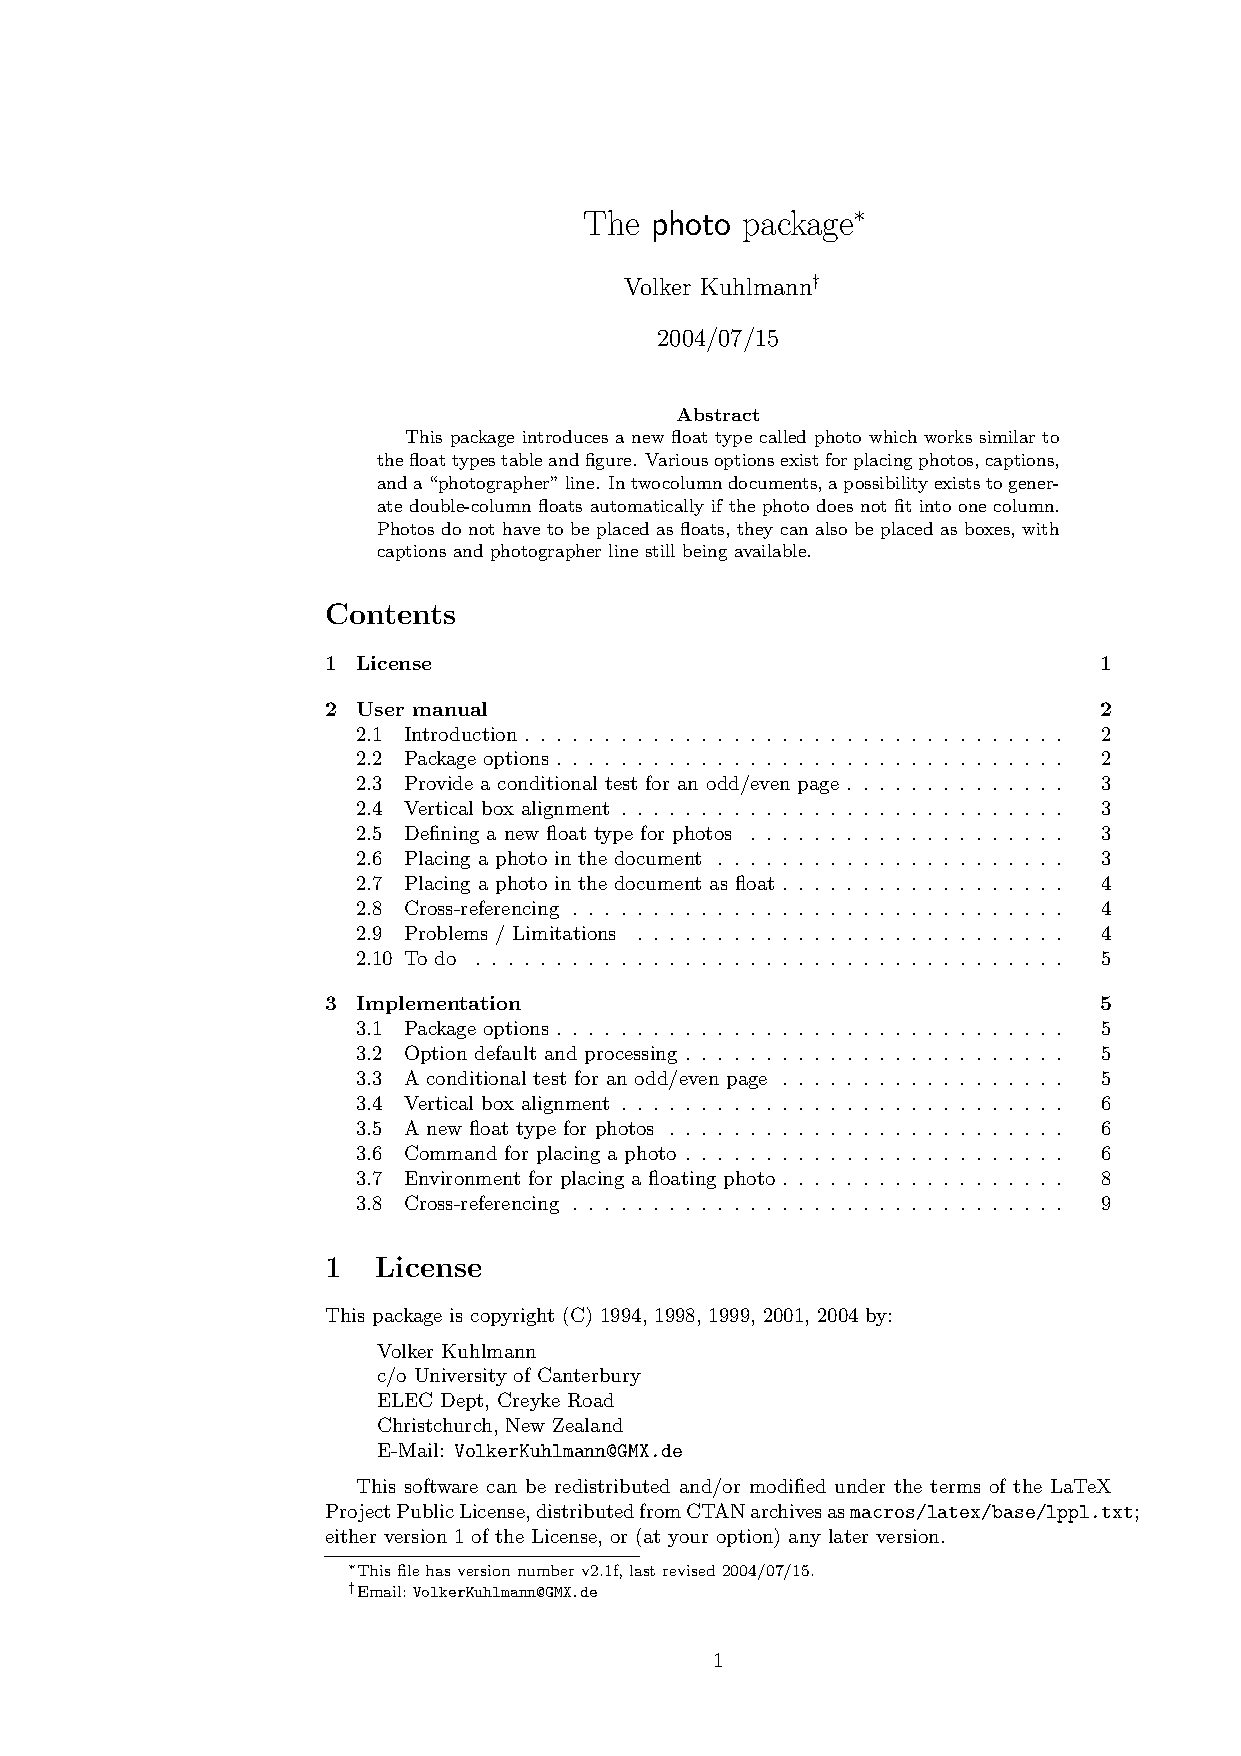
\includegraphics[bb=0 0 540 405]{photo.jpg}
\end{verbatim}
\end{quote}
It's usually not obvious what values to give the ``\texttt{bb}'' key,
but the program \ProgName{ebb} will generate a file
containing the information; the above numbers came from an
\ProgName{ebb} output file \File{photo.bb}:
\begin{quote}
\begin{verbatim}
%%Title: /home/gsm10/photo.jpg
%%Creator: ebb Version 0.5.2
%%BoundingBox: 0 0 540 405
%%CreationDate: Mon Mar  8 15:17:47 2004
\end{verbatim}
\end{quote}
However, if such a file is available, you may abbreviate the inclusion
code, above, to read:
\begin{quote}
\begin{verbatim}
\usepackage[dvipdfm]{graphicx}
...
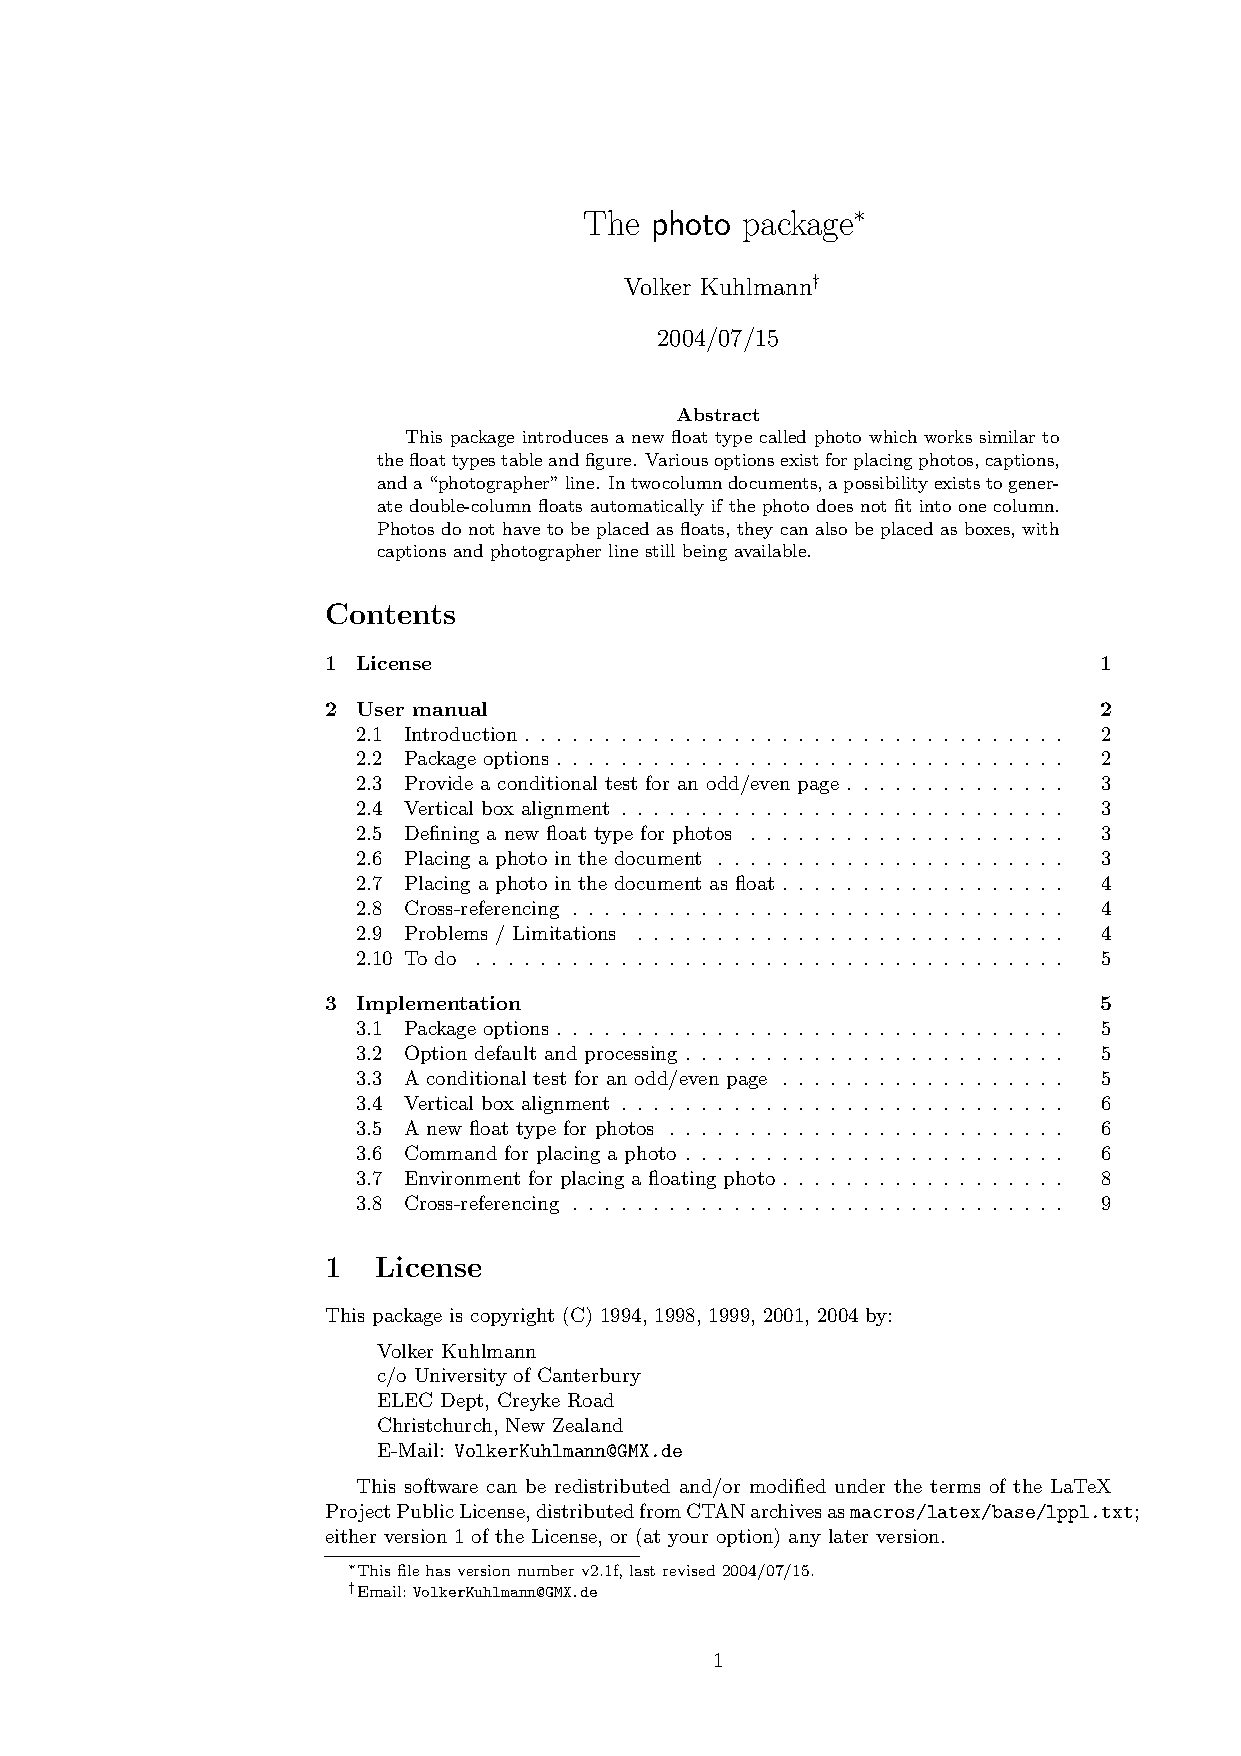
\includegraphics{photo}
\end{verbatim}
\end{quote}
which makes the operation feel as simple as does including
\texttt{.eps} images in a \LaTeX{} file for processing with
\ProgName{dvips}; the \Package{graphicx} package knows to look for a
\texttt{.bb} file if no bounding box is provided in the
\csx{includegraphics} command.

The one place where usage isn't quite so simple is the need to quote
\ProgName{dvipdfm} explicitly, as an option when loading the
\Package{graphicx} package: if you are using \ProgName{dvips}, you
don't ordinarily need to specify the fact, since the default graphics
configuration file (of most distributions) ``guesses'' the
\texttt{dvips} option if you're using \TeX{}.
\begin{ctanrefs}
\item[dvipdfm]\CTANref{dvipdfm}
\item[ebb]Distributed as part of \CTANref{dvipdfm}
\end{ctanrefs}

\Question[Q-graphicspath]{Importing graphics from ``somewhere else''}

By default, graphics commands like \csx{includegraphics} look
``wherever \TeX{} files are found'' for the graphic file they're being
asked to use.  This can reduce your flexibility if you choose to hold
your graphics files in a common directory, away from your \AllTeX{}
sources.

The simplest solution is to patch \TeX{}'s path, by changing the
default path.  On most systems, the default path is taken from the
environment variable \texttt{TEXINPUTS}, if it's present; you can adapt that
to take in the path it already has, by setting the variable to
\begin{quote}
\begin{verbatim}
TEXINPUTS=.:<graphics path(s)>:
\end{verbatim}
\end{quote}
on a Unix system; on a Windows system the separator will be ``\texttt{;}''
rather than ``\texttt{:}''.  The ``\texttt{.}'' is there to ensure
that the current directory is searched first; the trailing
``\texttt{:}'' says ``patch in the value of \texttt{TEXINPUTS} from
your configuration file, here''.

This method has the merit of efficiency (\AllTeX{} does \emph{all} of
the searches, which is quick), but it's always clumsy and may prove
inconvenient to use in Windows setups (at least).

The alternative is to use the \Package{graphics} package command
\csx{graphicspath}; this command is of course also available to users
of the \Package{graphicx} and the \Package{epsfig} packages.  The
syntax of \csx{graphicspath}'s one argument is slightly odd: it's a
sequence of paths (typically relative paths), each of which is
enclosed in braces.  A slightly odd sample, given in the
\Package{graphics} bundle documentation, is:
\begin{quote}
\begin{verbatim}
\graphicspath{{eps/}{tiff/}}
\end{verbatim}
\end{quote}
however, if the security checks on your \AllTeX{} system allow, the
path may be anything you choose (rather than strictly relative, like
those above); note that the trailing ``\texttt{/}'' \emph{is} required.

Be aware that \csx{graphicspath} does not affect the operations of
graphics macros other than those from the graphics bundle~--- in
particular, those of the outdated \Package{epsf} and
\Package{psfig} packages are immune.

The disadvantage of the \csx{graphicspath} method is inefficiency.  The
package will call \AllTeX{} once for each entry in the list, which is
itself slows things.  More seriously, \TeX{} remembers the file name,
thus effectively losing memory, every time it's
asked to look up a file, so a document that uses a huge number of
graphical inputs could be embarrassed by lack of memory.

If your document is split into a variety of directories, and each
directory has its associated graphics, the \Package{import} package
may well be the thing for you; see the discussion % beware line break
\latexhtml{of ``bits of document in other directories'' (}{in the question ``}%
\Qref{bits of document in other directories}{Q-docotherdir}%
\latexhtml{)}{''}.
\begin{ctanrefs}
\item[graphics \nothtml{\rmfamily}bundle]\CTANref{graphics}
\item[import.sty]\CTANref{import}
\end{ctanrefs}

\Question[Q-graph-pspdf]{Portable imported graphics}

A regular need is a document to be distributed in more than
one format: commonly both \PS{} and \acro{PDF}.  The
following advice is based on a post by one with much experience of
dealing with the problem of dealing with \acro{EPS} graphics in this
case.
\begin{itemize}
\item Don't specify a driver when loading loading whichever version of
  the \Package{graphics} package you use.  The scheme relies on the
  distribution's ability to decide which driver is going to be used:
  the choice is between \ProgName{dvips} and \PDFTeX{}, in this case.
  Be sure to exclude options \pkgoption{dvips}, \pkgoption{pdftex} and
  \pkgoption{dvipdfm} (\ProgName{dvipdfm} is not used in this scheme,
  but the aspirant \acro{PDF}-maker may be using it for his output,
  before switching to the scheme).
\item Use \cmdinvoke{includegraphics}[...]{filename} without
  specifying the extension (i.e., neither \texttt{.eps} nor
  \texttt{.pdf}).
\item For every \texttt{.eps} file you will be including, produce a
  \texttt{.pdf} version, as described in % beware line break
  \Qref[question]{Graphics in \PDFLaTeX{}}{Q-pdftexgraphics}.  Having
  done this, you will have two copies of each graphic (a \texttt{.eps}
  and a \texttt{.pdf} file) in your directory.
\item Use \PDFLaTeX{} (rather than
  \LaTeX{}--\ProgName{dvips}--distillation or
  \LaTeX{}--\ProgName{dvipdfm}) to produce your \acro{PDF} output.
\end{itemize}
\ProgName{Dvipdfm}'s charms are less than attractive here: the
document itself needs to be altered from its default
(\ProgName{dvips}) state, before \ProgName{dvipdfm} will process it.

\Question[Q-repeatgrf]{Repeated graphics in a document}

A logo or ``watermark'' image, or any other image that is repeated in
your document, has the potential to make the processed version of the
document unmanageably large.  The problem is, that the default
mechanisms of graphics usage add the image at every point it's to be
used, and when processed, the image appears in the output file at each
such point.

Huge \PS{} files are embarrassing; explaining \emph{why} such a file
is huge, is more embarrassing still.

The \Qref*{\File{epslatex} graphics tutorial}{Q-tutbitslatex}
describes a technique for avoiding the problem: basically, one
converts the image that's to be repeated into a \PS{} subroutine, and
load that as a \ProgName{dvips} prologue file.  In place of the image,
you load a file (with the same bounding box as the image) containing
no more than an invocation of the subroutine defined in the prologue.

The \File{epslatex} technique is tricky, but does the job.  Trickier
still is the neat scheme of converting the figure to a one-character
Adobe Type~3 outline font.  While this technique is for the ``real
experts'' only (the author of this answer has never even tried it), it has
potential for the same sort of space saving as the \File{epslatex}
technique, with greater flexibility in actual use.

More practical is Hendri Adriaens' \Package{graphicx-psmin}; you load
this \emph{in place} of \Package{graphicx}, so rather than:
\begin{quote}
\begin{verbatim}
\usepackage[<options>]{graphicx}
\end{verbatim}
\end{quote}
you will write:
\begin{quote}
\begin{verbatim}
\usepackage[<options>]{graphicx-psmin}
\end{verbatim}
\end{quote}
and at the start of your document, you write:
\begin{quote}
\begin{verbatim}
\loadgraphics[<bb>]{<list of graphics>}
\end{verbatim}
\end{quote}
and each of the graphics in the list is converted to an ``object'' for
use within the resulting \PS{} output.  (This is, in essence, an
automated version of the \File{epslatex} technique described above.)

Having loaded the package as above, whenever you use
\csx{includegraphics}, the command checks if the file you've asked for
is one of the graphics in \csx{loadgraphics}' list.  If so, the
operation is converted into a call to the ``object'' rather than a new
copy of the file; the resulting \PS{} can of course be \emph{much} smaller.

Note that the package requires a recent \ProgName{dvips}, version
5.95b (this version isn't~--- yet~--- widely distributed).

If your \PS{} is destined for conversion to \acro{PDF}, either by a
\ProgName{ghostscript}-based mechanism such as \ProgName{ps2pdf} or by
(for example) \ProgName{Acrobat} \ProgName{Distiller}, the issue isn't
so pressing, since the distillation mechanism will amalgamate graphics
objects whether or not the \PS{} has them amalgamated.  \PDFTeX{} does
the same job with graphics, automatically converting multiple uses
into references to graphics objects.
\begin{ctanrefs}
\item[graphicx-psmin.sty]\CTANref{graphicx-psmin}
\end{ctanrefs}

\Question[Q-grmaxwidth]{Limit the width of imported graphics}

Suppose you have graphics which may or may not be able to fit within
the width of the page; if they will fit, you want to set them at their
natural size, but otherwise you want to scale the whole picture so
that it fits within the page width.

You do this by delving into the innards of the graphics package (which
of course needs a little \LaTeX{} internals programming):
\begin{quote}
\begin{verbatim}
\makeatletter
\def\maxwidth{%
  \ifdim\Gin@nat@width>\linewidth
    \linewidth
  \else
    \Gin@nat@width
  \fi
}
\makeatother
\end{verbatim}
\end{quote}
This defines a ``variable'' width which has the properties you want.
Replace \csx{linewidth} if you have a different constraint on the width
of the graphic.

Use the command as follows:
\begin{quote}
\begin{verbatim}
\includegraphics[width=\maxwidth]{figure}
\end{verbatim}
\end{quote}

\Question[Q-topgraph]{Top-aligning imported graphics}

When \TeX{} sets a line of anything, it ensures that the base-line of
each object in the line is at the same level as the base-line of the
final object.  (Apart, of course, from \csx{raisebox} commands\dots{})

Most imported graphics have their base-line set at the bottom of the
picture.  When using packages such as \Package{subfig}, one often
wants to align figures by their tops.  The following odd little bit of
code does this:
\begin{quote}
\begin{verbatim}
\vtop{%
  \vskip0pt
  \hbox{%
    \includegraphics{figure}%
  }%
}
\end{verbatim}
\end{quote}
The \csx{vtop} primitive sets the base-line of the resulting object to
that of the first ``line'' in it; the \csx{vskip} creates the illusion
of an empty line, so \csx{vtop} makes the very top of the box into the
base-line.

In cases where the graphics are to be aligned with text, there is a
case for making the base-line one ex-height below the top of the box,
as in:
\begin{quote}
\begin{verbatim}
\vtop{%
  \vskip-1ex
  \hbox{%
    \includegraphics{figure}%
  }%
}
\end{verbatim}
\end{quote}
A more \LaTeX{}-y way of doing the job (somewhat innefficiently) uses
the \Package{calc} package:
\begin{quote}
\begin{verbatim}
\usepackage{calc}
...
\raisebox{1ex-\height}{\includegraphics{figure}}
\end{verbatim}
\end{quote}
(this has the same effect as the text-align version, above).

The fact is, \emph{you} may choose where the base-line ends up.  This
answer merely shows you sensible choices you might make.

\Question[Q-mpprologues]{Displaying \MP{} output in \ProgName{ghostscript}}

\MP{} ordinarily expects its output to be included in some context
where the `standard' \MF{} fonts (that you've specified) are already
defined~--- for example, as a figure in \TeX{} document.  If you're
debugging your \MP{} code, you may want to view it in
\ProgName{ghostscript} (or some other \PS{} previewer).  However,
the \PS{} `engine' in \ProgName{ghostscript} \emph{doesn't}
ordinarily have the fonts loaded, and you'll eperience an error such
as
\begin{quote}
\begin{verbatim}
Error: /undefined in cmmi10
\end{verbatim}
\end{quote}
There is provision in \MP{} for avoiding this problem: issue the
command \texttt{prologues := 2;} at the start of the \texttt{.mp} file.

Unfortunately, the \PS{} that \MP{} inserts in its output,
following this command, is incompatible with ordinary use of the
\PS{} in inclusions into \AllTeX{} documents, so it's best to
make the \texttt{prologues} command optional.  Furthermore, \MP{} takes a
very simple-minded approach to font encoding: since \TeX{} font
encodings regularly confuse sophisticated minds, this can prove
troublesome.  If you're suffering such problems (the symptom is that
characters disappear, or are wrongly presented) the only solution is
to view the `original' metapost output after processing through
\LaTeX{} and \ProgName{dvips}.

Conditional compilation may be done either
by inputting \File{MyFigure.mp} indirectly from a simple wrapper
\File{MyFigureDisplay.mp}:
\begin{quote}
\begin{verbatim}
prologues := 2;
input MyFigure
\end{verbatim}
\end{quote}
or by issuing a shell command such as
\begin{quote}
\begin{verbatim}
mp '\prologues:=2; input MyFigure'
\end{verbatim}
\end{quote}
(which will work without the quote marks if you're not using a Unix
shell).

A suitable \LaTeX{} route would involve processing
\File{MyFigure.tex}, which contains:
\begin{quote}
\begin{verbatim}
\documentclass{article}
\usepackage{graphicx}
\begin{document}
\thispagestyle{empty}
\includegraphics{MyFigure.1}
\end{document}
\end{verbatim}
\end{quote}
Processing the resulting \acro{DVI} file with the \ProgName{dvips}
command
\begin{quote}
\begin{verbatim}
dvips -E -o MyFigure.eps MyFigure
\end{verbatim}
\end{quote}
would then give a satisfactory Encapsulated \PS{} file.  This
procedure may be automated using the \ProgName{Perl} script
\ProgName{mps2eps}, thus saving a certain amount of tedium.

The Plain~\TeX{} user may use an adaptation of a jiffy of Knuth's, by
Dan Luecking.  Dan's version \Package{mpsproof.tex} will work under
\TeX{} to produce a \acro{DVI} file for use with \ProgName{dvips}, or
under \PDFTeX{} to produce a \acro{PDF} file, direct.  The output is
set up to look like a proof sheet.

A script application, \ProgName{mptopdf}, is available in recent
\AllTeX{} distributions: it seems fairly reliably to produce
\acro{PDF} from \MP{}, so may reasonably be considered an answer to
the question\dots{}
\begin{ctanrefs}
\item[mps2eps]\CTANref{mps2eps}
\item[mpsproof.tex]\CTANref{mpsproof}
\item[mptopdf]Part of \CTANref{pdftex-graphics}
\end{ctanrefs}

\Question[Q-drawing]{Drawing with \TeX{}}

There are many packages to do pictures in \AllTeX{} itself (rather than
importing graphics created externally), ranging from simple use of
\LaTeX{} \environment{picture} environment, through enhancements like
\ProgName{epic}, to 
sophisticated (but slow) drawing with \PiCTeX{}. Depending on your type
of drawing, and setup, here are a few systems you may consider:
\begin{itemize}
\item \Package{pict2e}; this was advertised in % !line break
  \Qref*{the \LaTeX{} manual}{Q-books}, but didn't appear for nearly
  ten years after publication of the book!  It removes all the petty
  niggles that surround the use of the \environment{picture}
  environment.  It therefore suffers \emph{only} from the rather
  eccentric drawing language of the environment, and is a far more
  useful tool than the original environment has ever been.  (Note that
  \Package{pict2e} supersedes David Carlisle's stop-gap
  \Package{pspicture}.)
\item \Package{pstricks}; this gives you access to all the power of
  \PS{} from \TeX{} itself, by sophisticated use of
  \Qref*{\csx{special} commands}{Q-specials}.  Since \PS{} is itself a
  pretty powerful programming language, this means there are many
  astounding things that can in principle be achieved.
  \Package{pstricks}' \csx{special}s are
  by default specific to \ProgName{dvips}, but V\TeX{} (both in its
  commercial and in its free versions) understands them.  \PDFTeX{}
  users may use \Package{pdftricks}, which (like
  \Package{epstopdf}~--- see % ! line break
  \Qref[question]{\PDFLaTeX{} graphics}{Q-pdftexgraphics}) generates
  \acro{PDF} files on the fly from \Package{pstricks} commands.  The
  documentation is good (you may browse it via the % ! line break
  \href{http://pstricks.tug.org/}{\Package{pstricks} page}
  on the \acro{TUG} web site).  There is also a mailing list
  (\mailto{pstricks@tug.org}) which you may
  \href{http://tug.org/mailman/listinfo/pstricks}{join}, or you may
  just
  browse the \href{http://tug.org/pipermail/pstricks/}{list archives}.
\item \Package{pgf}: while \Package{pstricks} is very powerful and
  convenient, using it with \PDFLaTeX{} is an awful fidget: if you
  simply want the graphical capabilities, \Package{pgf}, together with
  its rather pleasing ``user-oriented'' interface \Package{tikz}, may be a good
  bet for you.  While \acro{PDF} has (in essence) the same graphical
  capabilities as \PS{}, it isn't programmable; \Package{pgf} provides
  common \LaTeX{} commands that will utilise the graphical
  capabilities of both \PS{} and \acro{PDF} equally.
\item \MP{}; you liked \MF{}, but never got to grips with font files?
  Try \Qref*{\MP{}}{Q-MP}~---
  all the power of \MF{}, but it generates \PS{} figures; \MP{}
  is nowadays part of most serious \AllTeX{} distributions.  Knuth
  uses it for all his work\dots{}
\item \ProgName{Mfpic}; you liked \MF{}, but can't understand the
  language?  The package makes up \MF{} or \MP{} code for you
  within using familiar-looking \TeX{} macros.  Not \emph{quite} the
  full power of \MP{}, but a friendlier interface; of course, with
  \MP{} output, the results can be used equally well in either
  \LaTeX{} or \PDFLaTeX{}.
\item You liked \PiCTeX{} but don't have enough memory or time?  Look
  at Eitan Gurari's \Package{dratex}, which is as powerful as most
  other \TeX{} drawing packages, but is an entirely new
  implementation, which is not as hard on memory, is much more
  readable (and is fully documented).
\end{itemize}
\begin{ctanrefs}
\item[dratex.sty]\CTANref{dratex}
\item[mfpic]\CTANref{mfpic}
\item[pdftricks.sty]\CTANref{pdftricks}
\item[pspicture.sty]\CTANref{pspicture}
\item[pgf.sty]\CTANref{pgf}
\item[pict2e.sty]\CTANref{pict2e}
\item[pstricks]\CTANref{pstricks}
\item[tikz.sty]Distributed with \CTANref{pgf}
\end{ctanrefs}

\Question[Q-drawFeyn]{Drawing Feynman diagrams in \LaTeX{}}

Michael Levine's \Package{feynman} bundle for drawing the diagrams in
\LaTeXo{} is still available.

Thorsten Ohl's \Package{feynmf} is designed for use with current
\LaTeX{}, and works in
combination with \MF{} (or, in its \Package{feynmp} incarnation, with
\MP{}).  The \ProgName{feynmf} or
\ProgName{feynmp} package reads a description of the diagram written
in \TeX{}, and writes out code.  \MF{} (or \MP{}) can then produce a
font (or \PS{} file) for use in a subsequent \LaTeX{} run.  For
new users, who have access to \MP{}, the \PS{} version is
probably the better route, for document portability and other reasons.
% checked rf 2001/03/22

Jos Vermaseren's \Package{axodraw} is mentioned as an alternative in
the documentation of \Package{feynmf}, but it is written entirely in
terms of \ProgName{dvips} \csx{special} commands, and is thus rather
imperfectly portable.

An alternative approach is implemented by Norman Gray's \Package{feyn}
package.  Rather than creating complete diagrams as postscript images,
\Package{feyn} provides a font (in a variety of sizes) containing
fragments, which you can compose to produce complete diagrams.  It
offers fairly simple diagrams which look good in equations, rather
than complicated ones more suitable for display in figures.
\begin{ctanrefs}
\item[axodraw]\CTANref{axodraw}
\item[feyn \nothtml{\rmfamily}font bundle]\CTANref{feyn}
\item[feynman bundle]\CTANref{feynman}
\item[feynmf/feynmp bundle]\CTANref{feynmf}
\end{ctanrefs}

\Question[Q-labelfig]{Labelling graphics}

``Technical'' graphics (such as graphs and diagrams) are often
labelled with quite complex mathematical expressions: there are few
drawing or graphing tools that can do such things (the honourable
exception being \MP{}, which allows you to program the labels, in
\AllTeX{}, in the middle of specifying your graphic).

Labels on graphics produced by all those \emph{other} tools is where
the \Package{psfrag} package can help.  Place an unique
text in your graphic, using the normal text features of your tool, and
you can ask \Package{psfrag} to replace the text with arbitrary
\AllTeX{} material.  \Package{Psfrag}'s ``operative'' command is
\cmdinvoke{psfrag}{\emph{PS text}}{\emph{Repl text}}, which instructs
the system to replace the original (``\texttt{PS}'') text with the
\TeX{}-typeset replacement text.  Optional
arguments permit adjustment of position, scale and rotation; full
details may be found in \File{pfgguide} in the distribution.
(Unfortunately, \Package{psfrag} can't be used with \PDFLaTeX{},
though one might hope that it would be susceptible to the same sort of
treatment as is used in the \Package{pdftricks} package.  On the other
hand,
\begin{narrowversion}
  V\TeX{}'s GeX processor (\Qref{}{Q-commercial})
\end{narrowversion}
\begin{wideversion}
  \Qref*{V\TeX{}}{Q-commercial}'s GeX processor
\end{wideversion}
explicitly deals with \Package{psfrag}, both in its free and
commercial instances.)

The \Package{psfragx} package goes one step further than
\Package{psfrag}: it provides a means whereby you can put the
\Package{psfrag} commands into the preamble of your \acro{EPS} file
itself.  \Package{Psfrag} has such a command itself, but deprecates
it; \Package{psfragx} has cleaned up the facility, and provides a
script \ProgName{laprint} for use with \ProgName{Matlab} to produce
appropriately tagged output.  (In principle, other graphics
applications could provide a similar facility, but apparently none does.)

\ProgName{Emacs} users may find the embedded editor \ProgName{iTe} a
useful tool for placing labels: it's a \AllTeX{}-oriented graphical
editor written in \ProgName{Emacs Lisp}.  You create
\environment{iteblock} environments containing graphics and text, and
may then invoke \ProgName{iTe} to arrange the elements relative to one
another.

Another useful approach is \Package{overpic}, which overlays a
\environment{picture} environment on a graphic included by use of
\csx{includegraphics}.  This treatment lends itself to ready placement
of texts and the like on top of a graphic.  The package can draw a
grid for planning your ``attack''; the distribution comes with simple
examples.

\Package{Pstricks} can of course do everything that \Package{overpic}
can, with all the flexibility of \PS{} programming that it offers
The \Package{pstricks} web site has a page with several % ! line break
\href{http://pstricks.tug.org/main.cgi?file=Examples/overlay}{examples of labelling}
which will get you started; if \Package{pstricks} is % ! line break
\Qref*{an option for you}{Q-drawing}, this route is worth a try.

The confident user may, of course, do the whole job in a picture
environment which itself includes the graphic.  I would recommend
\Package{overpic} or the \Package{pstricks} approach, but such things
are plainly little more than a convenience over what is achievable
with the do-it-yourself approach.
\begin{ctanrefs}
\item[iTe]\CTANref{ite}
\item[laprint]Distributed with \CTANref{psfragx}
\item[overpic.sty]\CTANref{overpic}
\item[psfrag.sty]\CTANref{psfrag}
\item[psfragx.sty]\CTANref{psfragx}
\item[pstricks.sty]\CTANref{pstricks}
\end{ctanrefs}

%%%%%%%%%%%%%%%%%%%%%%%%%%%%%%%%%%%%%%%%%%%%%%%%%%%%%%%%%%%%%%%%%

\section{Bibliographies and citations}

\subsection{Creating bibliographies}

\Question[Q-buildbib]{Creating a \BibTeX{} bibliography file}

A \BibTeX{} bibliography file may reasonably be compared to a small
database, the entries in which are references to literature that may
be called up by citations in a document.

Each entry in the bibliography has a \emph{type} and a unique
\emph{key}.  The bibliography is read, by \BibTeX{}, using the details
specified in a \emph{bibliography style}.  From the style, \BibTeX{}
finds what entry types are permissible, what \emph{fields} each entry
type has, and how to format the whole entry.

The type specifies the type of document you're making reference to; it
may run all the way from things like ``\environment{Book}'' and
``\environment{Proceedings}'' (which may even contain other citations
of type ``\environment{InBook}'' or  ``\environment{InProceedings}'')
through dissertation styles like  ``\environment{PhdThesis}'' to
otherwise-uncategorisable things such as ``\environment{Misc}''.  The
unique key is something you choose yourself: it's what you use when
you want to \Qref*{cite an entry in the file}{Q-usebibtex}.  People
commonly create a key that combines the (primary) author's name and
the year of publication, possibly with a marker to distinguish
publications in the same year.  So, for example, the Dyson, Eddington,
Davidson paper about deflection of starlight appears in my
experimental \texttt{.bib} file as \texttt{Dyson20.1}.

So, noting the rules of the style, you have `simply' to write a
bibliography database.  Fortunately, there are several tools to help
in this endeavour:
\begin{itemize}
\item Most of the better \Qref*{\AllTeX{}-oriented editors}{Q-editors}
  have ``\BibTeX{} modes''.
\item If you have an existing \environment{thebibliography}
  environment, the \ProgName{Perl} script \ProgName{tex2bib} will
  probably help.
\item There are a number of \BibTeX{} bibliography management systems
  available, some of which permit a graphical user interface to the
  task.  Sadly, none seems to be available with the ordinary \TeX{}
  distributions.
  
  Tools such as \ProgName{Xbibfile} (a graphical user interface),
  \ProgName{ebib} (a database application written to run `inside'
  \ProgName{emacs}) and 
  \ProgName{btOOL} (a set of \ProgName{perl} tools for building 
  \BibTeX{} database handlers) are available from \acro{CTAN}.

  Other systems, such as
  \href{http://refdb.sourceforge.net/}{\ProgName{RefDB}},
  \href{http://www.nongnu.org/biborb}{BibORB},
  \href{http://bibdesk.sourceforge.net/}{\ProgName{BibDesk}},
  \href{http://pybliographer.org}{\ProgName{pybliographer}} and the
  \ProgName{Java}-based
  \href{http://freshmeat.net/projects/bibkeeper/}{\ProgName{Bibkeeper}}
  and \href{http://jabref.sourceforge.net}{\ProgName{JabRef}} (which
  claims to supersede \ProgName{Bibkeeper})
  are only available from their development sites.
% review of web database offerings in textex_368
\item Some commercial citation-management systems will export in
  \BibTeX{} format; an example is
  \href{http://www.endnote.com/}{EndNote}.
\item Data from on-line citation databases may often be translated to
  \BibTeX{} format by utilities to be found on \acro{CTAN}.  For
  example, the \ProgName{Perl} script \ProgName{isi2bibtex} will
  translate citations from \acro{ISI} ``Web of knowledge'' (a
  subscription service, available to \acro{UK} academics via
  \acro{BIDS}).  UK academics may translate \acro{BIDS} downloads
  using \ProgName{bids.to.bibtex}
\end{itemize}
\begin{ctanrefs}
\item[bids.to.bibtex]\CTANref{bidstobibtex}
\item[btOOL]\CTANref{btOOL}
\item[ebib]\CTANref{ebib}
\item[isi2bibtex]\CTANref{isi2bibtex}
\item[tex2bib]\CTANref{tex2bib}
\item[tex2bib.readme]\CTANref{tex2bib-doc}
\item[xbibfile]\CTANref{xbibfile}
\end{ctanrefs}

\Question[Q-custbib]{Creating a bibliography style}

It \emph{is} possible to write your own: the standard bibliography
styles are distributed in a commented form, and there is a description
of the language (see
% beware line-wrap
\Qref[question]{BibTeX documentation}{Q-BibTeXing}).
However, it must be admitted that the language in which \BibTeX{}
styles are written is pretty obscure, and one would not recommend
anyone who's not a confident programmer to write their own, though
minor changes to an existing style may be within the grasp of many.

If your style isn't too `far out', you can probably generate it by
using the facilities of the \Package{custom-bib} bundle.  This
contains a file \File{makebst.tex}, which runs you through a text menu
to produce a file of instructions, with which you can generate your
own \texttt{.bst} file.  This technique doesn't offer entirely new styles
of document, but the system's ``master \BibTeX{} styles'' already
offer significantly more than the \BibTeX{} standard set.
\begin{ctanrefs}
\item[\nothtml{\normalfont}\BibTeX{} documentation]\CTANref{bibtex-doc}
\item[makebst.tex]Distributed with \CTANref{custom-bib}
\end{ctanrefs}

\Question[Q-capbibtex]{Capitalisation in \BibTeX{}}

The standard \BibTeX{} bibliography styles impose fixed ideas about
the capitalisation of titles of things in the bibliography.  While
this is not unreasonable by \BibTeX{}'s lights (the rules come from
the \emph{Chicago Manual of Style}) it can be troublesome, since
\BibTeX{} fails to recognise special uses (such as acronyms, chemical
formulae, etc.).

The solution is to enclose the letter or letters, whose capitalisation
\BibTeX{} should not touch, in braces, as:
\begin{quote}
\begin{verbatim}
title = {The {THE} operating system},
\end{verbatim}
\end{quote}
Sometimes you find \BibTeX{} changing the case of a single letter
inappropriately.  No matter: the technique can be applied to single
letters, as in:
\begin{quote}
\begin{verbatim}
title = {Te{X}niques and tips},
\end{verbatim}
\end{quote}
If your document design specification requires a different style of
capitalisation, you should acquire a bibliography style that doesn't
enforce \BibTeX{}'s default rules.  It is definitely \emph{not} a good
idea to enclose an entire title in braces, as in
\begin{quote}
\begin{verbatim}
title = {{TeXniques and tips}},
\end{verbatim}
\end{quote}
though that does ensure that the capitalisation is not changed.  Your
\BibTeX{} database should be a general-purpose thing, not something
tuned to the requirements of a particular document, or to the way you
are thinking today.

There's more on the subject in the
% beware line wrap
\Qref*{\BibTeX{} documentation}{Q-BibTeXing}.

\Question[Q-bibaccent]{Accents in bibliographies}

\BibTeX{} not only has a tendency (by default) to mess about with the
% line wrap
\Qref*{case of letters in your bibliography}{Q-capbibtex},
also makes a hash of accent commands:
\begin{htmlversion}
``\texttt{ma\~nana}'' comes out as ``ma nana'' (!).  The solution is
similar: enclose the troublesome sequence in braces, as
``|{|\texttt{\~n}|}|'', in this example.
\end{htmlversion}
\htmlignore
``|ma\~nana|'' comes out as ``ma nana'' (!).  The solution is similar:
enclose the troublesome sequence in braces, as ``|{\~n}|'', in this
example.
\endhtmlignore

\Question[Q-bibstrtl]{`String too long' in \BibTeX{}}

The \BibTeX{} diagnostic ``Warning--you've exceeded 1000, the
\texttt{global-string-size}, for entry \texttt{foo}'' usually arises
from a very large abstract or annotation included in the database.
The diagnostic usually arises because of an infelicity in the coding of
\File{abstract.bst}, or styles derived from it.  (One doesn't
ordinarily output annotations in other styles.)

The solution is to make a copy of the style file (or get a clean copy
from \acro{CTAN}~--- \CTANref{abstract-bst}), and rename it (e.g., on a
long file-name system, to \File{abstract-long.bst}).  Now edit it: find
function \texttt{output.nonnull} and
\begin{itemize}
\item change its first line (line 60 in the version on \acro{CTAN})
  from
  \begin{quote}
\begin{verbatim}
{ 's :=
\end{verbatim}
  \end{quote}
to
  \begin{quote}
\begin{verbatim}
{ swap$
\end{verbatim}
  \end{quote}
  Finally,
\item delete the function's last line, which just says ``\texttt{s}
  (line 84 in the version on \acro{CTAN}).
\end{itemize}
Finally, change your \csx{bibliographystyle} command to refer to the
name of the new file.

This technique applies equally to any bibliography style: the same
change can be made to any similar \texttt{output.nonnull} function.

If you're reluctant to make this sort of change, the only way forward
is to take the entry out of the database, so that you don't encounter
\BibTeX{}'s limit, but you may need to retain the entry because it
will be included in the typeset document.  In such cases, put the body
of the entry in a separate file:
\begin{quote}
\begin{verbatim}
@article{long.boring,
  author =    "Fred Verbose",
  ...
  abstract =  "{\input{abstracts/long.tex}}"
}
\end{verbatim}
\end{quote}
In this way, you arrange that all \BibTeX{} has to deal with is the
file name, though it will tell \TeX{} (when appropriate) to include
all the long text.

\Question[Q-manyauthor]{\BibTeX{} doesn't understand lists of names}

\BibTeX{} has a strict syntax for lists of authors' (or editors')
names in the \BibTeX{} data file; if you write the list of names in a
``natural''-seeming way, the chances are you will confuse \BibTeX{},
and the output produced will be quite different from what you had
hoped.

Names should be expressed in one of the forms
\begin{quote}
\begin{verbatim}
First Last
Last, First
Last, Suffix, First
\end{verbatim}
\end{quote}
and lists of names should be separated with ``\texttt{and}''.
For example:
\begin{quote}
\begin{verbatim}
AUTHOR = {Fred Q. Bloggs, John P. Doe \&
          Another Idiot}
\end{verbatim}
\end{quote}
falls foul of two of the above rules: a syntactically significant
comma appears in an incorrect place, and `\csx{\&}' is being used as a
name separator.  The output of the above might be something like:
\begin{quote}
\begin{wideversion}
\begin{verbatim}
John P. Doe \& Another Idiot Fred Q. Bloggs
\end{verbatim}
\end{wideversion}
\begin{narrowversion}
\begin{verbatim}
John P. Doe \& Another Idiot
                        Fred Q. Bloggs
\end{verbatim}
\end{narrowversion}
\end{quote}
because ``John P. Doe \& Another Idiot has become the `first name',
while ``Fred Q. Bloggs'' has become the `last name' of a single
person.  The example should have been written:
\begin{quote}
\begin{narrowversion}
\begin{verbatim}
AUTHOR = {Fred Q. Bloggs and
          John P. Doe and
          Another Idiot}
\end{verbatim}
\end{narrowversion}
\begin{wideversion}
\begin{verbatim}
AUTHOR = {Fred Q. Bloggs and John P. Doe and
          Another Idiot}
\end{verbatim}
\end{wideversion}
\end{quote}
Some bibliography styles implement clever acrobatics with very long
author lists.  You can force truncation by using the pseudo-name
``|others|'', which will usually translate to something like
``\emph{et al}'' in the typeset output.  So, if Mr.~Bloggs wanted to
distract attention from his co-authors, he would write:
\begin{quote}
\begin{verbatim}
AUTHOR = {Fred Q. Bloggs and others}
\end{verbatim}
\end{quote}

\Question[Q-citeURL]{\acro{URL}s in \BibTeX{} bibliographies}

There is no citation type for \acro{URL}s, \emph{per se}, in the
standard \BibTeX{} styles, though Oren Patashnik (the author of
\BibTeX{}) is believed to beconsidering developing one such for use
with the long-awaited \BibTeX{} version~1.0.

The actual information that need be available in a citation of an
\acro{URL} is discussed at some length in the publicly available
on-line 
\begin{narrowversion}
  extracts of \acro{ISO}~690--2, available via
  \URL{http://www.nlc-bnc.ca/iso/tc46sc9/standard/690-2e.htm};
  % checked 2004-01-15
\end{narrowversion}
\begin{wideversion}
\href{http://www.nlc-bnc.ca/iso/tc46sc9/standard/690-2e.htm}{extracts of \acro{ISO}\nobreakspace690--2};
\end{wideversion}
the techniques below do \emph{not} satisfy all the requirements of
\acro{ISO}~690--2, but they offer a solution that is at least
available to users of today's tools.

Until the new version of \BibTeX{} arrives, the simplest technique is
to use the \texttt{howpublished} field of the standard styles' \texttt{@misc}
function.  Of course, the strictures
about \Qref*{typesetting \acro{URL}s}{Q-setURL} still apply, so the
entry will look like:
\begin{quote}
\begin{verbatim}
@misc{...,
  ...,
  howpublished = "\url{http://...}"
}
\end{verbatim}
\end{quote}
A possible alternative approach is to use \BibTeX{} styles other than
the standard ones, that already have \acro{URL} entry types.
Candidates are:
\begin{itemize}
\item The \Package{natbib} styles (\Package{plainnat},
  \Package{unsrtnat} and \Package{abbrevnat}), which are extensions of
  the standard styles, principally for use with \Package{natbib}
  itself.  However, they've acquired \acro{URL}s and other ``modern''
  entries along the way.  The same author's \Package{custom-bib} is
  also capable of generating styles that honour \acro{URL} entries.
\item The \Package{babelbib} bundle, which offers % ! line break
  \Qref*{multilingual bibliographies}{Q-i18nbib}, similarly provides a
  set of standard-style equivalents that have \acro{URL} entries.
\item More modern styles such as the \Package{harvard} package (if the
  citation styles are otherwise satisfactory for you).
  \Package{Harvard} bibliography styles all include a ``\texttt{url}''
  field in their specification; however, the typesetting offered is
  somewhat feeble (though it does recognise and use
  \ProgName{LaTeX2HTML} macros if they are available, to create
  hyperlinks).
\end{itemize}
You can also acquire new \BibTeX{} styles by use of Norman Gray's
\Package{urlbst} system, which is based on a \ProgName{Perl} script
that edits an existing \BibTeX{} style file to produce a new
style. The new style thus generated has a |webpage| entry type, and
also offers support for |url| and |lastchecked| fields in the other entry
types.  The \ProgName{Perl} script comes with a set of converted
versions of the standard bibliography styles.  Documentation is
distributed as \LaTeX{} source.

Another possibility is that some conventionally-published paper,
technical report (or even book) is also available on the Web.  In such
cases, a useful technique is something like:
\begin{quote}
\begin{wideversion}
\begin{verbatim}
@techreport{...,
  ...,
  note = "Also available as \url{http://...}"
}
\end{verbatim}
\end{wideversion}
\begin{narrowversion}
\begin{verbatim}
@techreport{...,
  ...,
  note = "Also available as 
                       \url{http://...}"
}
\end{verbatim}
\end{narrowversion}
\end{quote}
There is good reason to use the \Package{url} or \Package{hyperref}
packages in this context: \BibTeX{} has a habit of splitting
lines it considers excessively long, and if there are no space
characters for it to use as `natural' breakpoints, \BibTeX{} will
insert a comment (`\texttt{\textpercent}') character~\dots{}\@ which
is an acceptable character in an \acro{URL}.  Any current version of the
\Package{url} or \Package{hyperref} package detects this
``\texttt{\textpercent}--end-of-line'' structure in its argument, and
removes it.
\begin{ctanrefs}
\item[babelbib \nothtml{\rmfamily}bundle]\CTANref{babelbib}
\item[custom-bib \nothtml{\rmfamily}bundle]\CTANref{custom-bib}
\item[harvard.sty]\CTANref{harvard}
\item[hyperref.sty]\CTANref{hyperref}
\item[natbib \nothtml{\rmfamily}styles]\CTANref{natbib}
\item[url.sty]\CTANref{url}
\item[urlbst]\CTANref{urlbst}
\end{ctanrefs}

\Question[Q-bibplain]{Using \BibTeX{} with Plain \TeX{}}

The file \File{btxmac.tex} (which is part of the \Eplain{} system)
contains macros and documentation for using \BibTeX{} with Plain
\TeX{}, either directly or with \Qref*{\Eplain{}}{Q-eplain}.  See
\Qref[question]{the use of \BibTeX{}}{Q-BibTeXing} for more
information about \BibTeX{} itself.
\begin{ctanrefs}
\item[btxmac.tex]\CTANref{btxmactex}
\item[eplain \nothtml{\rmfamily}system]\CTANref{eplain}
\end{ctanrefs}

\Question[Q-makebib]{Reconstructing \texttt{.bib} files}

Perhaps you've lost the \texttt{.bib} file you generated your document from,
or have been sent a document without one.  Or even, you've realised
the error of building a substantial document without the benefit of
\BibTeX{}\dots{}

The \ProgName{Perl} script, \Package{tex2bib} makes a reasonable job
of regenerating |.bib| files from \environment{thebibliography}
environments, provided that the original (whether automatically or
manually generated) doesn't deviate too far from the ``standard''
styles.

You are well-advised to check the output of the script.  While it will
not usually destroy information, it can quite reasonably mislabel it.

Documentation of the script is to be found in the file \File{tex2bib.readme}
\begin{ctanrefs}
\item[tex2bib]\CTANref{tex2bib}
\item[tex2bib.readme]\CTANref{tex2bib-doc}
\end{ctanrefs}

\Question[Q-bibprefixsort]{\BibTeX{} sorting and name prefixes}

\BibTeX{} recognises a bewildering array of name prefixes (mostly
those deriving from European language names); it ignores the prefixes
when sorting the bibliography~--- you want ``Ludwig van Beethoven''
sorted under ``Beethoven'', not under ``van''.  (Lamport made a witty
deliberate mistake with Beethoven's name, in the first edition of his
\LaTeX{} manual.)

However, a recurring issue is the desire to quote Lord Rayleigh's
publications (``Lord'' isn't an acceptable prefix), or names from
languages that weren't considered when \BibTeX{} was designed such as
``al-Wakil'' (transcribed from the Arabic).  What's needed is a
separate ``sort key'', but \BibTeX{} only allows such a thing in
citations of items that have no author or editor.

The solution is to embed the sort key in the author's name, but to
prevent it from being typeset.  Patashnik recommends a command
\csx{noopsort} (no-output-sortkey), which is defined and used as
follows:
\begin{quote}
\begin{wideversion}
\begin{verbatim}
@PREAMBLE{ {\providecommand{\noopsort}[1]{}} }
...
@ARTICLE{Rayleigh1,
AUTHOR = "{\noopsort{Rayleigh}}{Lord Rayleigh}",
...
}
\end{verbatim}
\end{wideversion}
\begin{narrowversion}
\begin{verbatim}
@PREAMBLE{
    {\providecommand{\noopsort}[1]{}}
}
...
@ARTICLE{Rayleigh1,
AUTHOR = 
   "\noopsort{Rayleigh}{Lord Rayleigh}",
...
}
\end{verbatim}
\end{narrowversion}
\end{quote}
Note that this \csx{noopsort} applies to the last name in this kind of
construct, so an author with an Arabic name might be rendered:
\begin{wideversion}
\begin{quote}
\begin{verbatim}
...
AUTHOR = "Ali {\noopsort{Hadiidii}}{al-Hadiidii}",
...
\end{verbatim}
\end{quote}
\end{wideversion}
\begin{narrowversion}
\begin{quote}
\begin{verbatim}
...
AUTHOR = 
   "Ali {\noopsort{Hadiidii}}{al-Hadiidii}",
...
\end{verbatim}
\end{quote}
\end{narrowversion}
A further use might deal with word order games, as in the famous
Vietnamese name:
\begin{wideversion}
\begin{quote}
\begin{verbatim}
...
AUTHOR = "\noopsort{Thanh Han The}{Han The Thanh}",
...
\end{verbatim}
\end{quote}
\end{wideversion}
\begin{narrowversion}
\begin{quote}
\begin{verbatim}
...
AUTHOR =
   "\noopsort{Thanh Han The}{Han The Thanh}",
...
\end{verbatim}
\end{quote}
\end{narrowversion}
though that author seems well-acquainted with Western confusion about
the significance of the parts of his name (even to the extent of
missing out the accentuation, as above\dots{}).

\Question[Q-bibtranscinit]{Transcribed initials in \BibTeX{}}

If your bibliographic style uses initials~+ surname, you may encounter
a problem with some transcribed names (for example, Russian ones).
Consider the following example from the real world:
\begin{quote}
\begin{narrowversion}
\begin{verbatim}
@article{epifanov1997,
   author = {Epifanov, S. Yu. and
             Vigasin, A. A.},
   title  = ...
}
\end{verbatim}
\end{narrowversion}
\begin{wideversion}
\begin{verbatim}
@article{epifanov1997,
   author = {Epifanov, S. Yu. and Vigasin, A. A.},
   title  = ...
}
\end{verbatim}
\end{wideversion}
\end{quote}
Note that the ``Yu'' is the initial, not a complete name. However,
\BibTeX{}'s algorithms will leave you with a citation~--- 
slightly depending on the bibliographic style~--- that reads:
``S. Y. Epifanov and A. A. Vigasin, \dots{}''. instead of the intended
``S. Yu. Epifanov and A. A. Vigasin, \dots{}''.

One solution is to replace each affected initial by a command that 
prints the correct combination.  To keep your bibliography portable,
you need to add that command to your bibliography with the
\texttt{@preamble} directive:
\begin{quote}
\begin{narrowversion}
\begin{verbatim}
@preamble{ {\providecommand{\BIBYu}{Yu} } }

@article{epifanov1997,
   author   = {Epifanov, S. {\BIBYu}. and
               Vigasin, A. A.},
   title    = ...
}
\end{verbatim}
\end{narrowversion}
\begin{wideversion}
\begin{verbatim}
@preamble{ {\providecommand{\BIBYu}{Yu} } }

@article{epifanov1997,
   author   = {Epifanov, S. {\BIBYu}. and Vigasin, A. A.},
   title    = ...
}
\end{verbatim}
\end{wideversion}
\end{quote}
If you have many such commands, you may want to put them in a separate
file and \csx{input} that \LaTeX{} file in a \texttt{@preamble}
directive.

An alternative is to make the transcription look like an accent, from
\BibTeX{}'s point of view.  For this we need a control sequence that
does nothing:
\begin{quote}
\begin{verbatim}
@article{epifanov1997,
   author   = {Epifanov, S. {\relax Yu}. and Vigasin, A. A.},
   title    = ...
}
\end{verbatim}
\end{quote}
Like the solution by generating extra commands, this involves tedious
extra typing; which of the two techniques is preferable for a given
bibliography will be determined by the names in it.

\subsection{Creating citations}

\Question[Q-usebibtex]{``Normal'' use of \BibTeX{} from \LaTeX{}}

To create a bibliography for your document, you need to perform a
sequence of steps, some of which seem a bit odd.  If you choose to use
\BibTeX{}, the sequence is:

First: you need a \BibTeX{} bibliography file (a |.bib| file)~--- see
\nothtml{``creating a \BibTeX{} file'' (\Qref[question]{}{Q-buildbib}).}
\begin{htmlversion}
``\Qref[question]{creating a \BibTeX{} file}{Q-buildbib}''.
\end{htmlversion}

Second: you must write your \LaTeX{} document to include a declaration
of the `style' of bibliography, citations, and a reference to the
bibliography file mentioned in the step 1.  So we may have a \LaTeX{}
file containing:
\begin{quote}
\begin{verbatim}
\bibliographystyle{plain}
...
Pooh is heroic~\cite{Milne:1926}.
...
Alice struggles~\cite{Carroll:1865}.
...
\bibliography{mybooks}
\end{verbatim}
\end{quote}
Note: we have bibliography style \Package{plain}, above, which is
nearly the simplest of the lot: a sample text, showing the sorts of
style choices available, can be found on Ken Turner's web site:
\URL{http://www.cs.stir.ac.uk/~kjt/software/latex/showbst.html}

Third: you must process the file.
\begin{quote}
\begin{verbatim}
latex myfile
\end{verbatim}
\end{quote}
As \LaTeX{} processes the file, the \csx{bibliographystyle} command
writes a note of the style to the |.aux| file; each \csx{cite} command
writes a note of the citation to the |.aux| file, and the
\csx{bibliography} command writes a note of which |.bib| file is to be
used, to the |.aux| file.

Note that, at this stage, \LaTeX{} isn't ``resolving'' any of the
citations: at every \csx{cite} command, \LaTeX{} will warn you of the
undefined citation, and when the document finishes, there will be a
further warning of undefined references.

%Some bibliography styles are designed to work with particular
%packages...

Fourth: you must run \BibTeX{}:
\begin{quote}
\begin{verbatim}
bibtex myfile
\end{verbatim}
\end{quote}
Don't try to tell \BibTeX{} anything but the file name: say
\texttt{bibtex myfile.aux} (because you know it's going to read the
|.aux| file) and \BibTeX{} will blindly attempt to process
\texttt{myfile.aux.aux}.

\BibTeX{} will scan the |.aux| file; it will find which bibliography
style it needs to use, and will ``compile'' that style; it will note
the citations; it will find which bibliography files it needs, and
will run through them matching citations to entries in the
bibliography; and finally it will sort the entries that have been
cited (if the bibliography style specifies that they should be
sorted), and outputs the resulting details to a |.bbl| file.

Fifth: you run \LaTeX{} again.  It warns, again, that each citation is
(still) undefined, but when it gets to the \csx{bibliography} command,
it finds a |.bbl| file, and reads it.  As it encounters each
\csx{bibitem} command in the file, it notes a definition of the
citation.

Sixth: you run \LaTeX{} yet again.  This time, it finds values for all
the citations, in its |.aux| file.  Other things being equal, you're
done\dots{} until you change the file.

If, while editing, you change any of the citations, or add new ones,
you need to go through the process above from steps 3 (first run of
\LaTeX{}) to 6, again, before the document is once again stable.
These four mandatory runs of \LaTeX{} make processing a document with
a bibliography even more tiresome than the normal two runs required to
resolve labels.

To summarise: processing to resolve citations requires: \LaTeX{};
\BibTeX{}; \LaTeX{}; \LaTeX{}.

\Question[Q-whatbst]{Choosing a bibliography style}

A large proportion of people are satisfied with one of Patashnik's
original ``standard'' styles, \Package{plain}, \Package{unsrt},
\Package{abbrv} and \Package{alpha}.  However, no style in that set
supports the ``author-date'' citation style that is popular in many
fields; but there are a very large number of contributed styles
available, that \emph{do} support the format.

(Note that author-date styles arose because the simple and clear
citation style that \Package{plain} produces is so awkward in a
traditional manuscript preparation scenario.  However, \TeX{}-based
document production does away with all those difficulties, leaving us
free once again to use the simple option.)

Fortunately, help is at hand, on the Web, with this problem:
\begin{itemize}
\item a sample text, showing the sorts of style choices available, can
  be found on 
\begin{narrowversion}
  Ken Turner's web site:
  \URL{http://www.cs.stir.ac.uk/~kjt/software/latex/showbst.html};
\end{narrowversion}
\begin{wideversion}
  % ! line break
  \href{http://www.cs.stir.ac.uk/~kjt/software/latex/showbst.html}{Ken Turner's web site};
\end{wideversion}
\item an excellent survey, that lists a huge variety of styles,
  sorted into their nominal topics as well as providing a good range
  of examples, is the Reed College % ! line break
\begin{narrowversion}
  ``Choosing a \BibTeX{} style''
  (\URL{http://web.reed.edu/cis/help/LaTeX/bibtexstyles.html}).
\end{narrowversion}
\begin{wideversion}
  % ! line break
  ``\href{http://web.reed.edu/cis/help/LaTeX/bibtexstyles.html}{Choosing a \BibTeX{} style}''.
\end{wideversion}
\end{itemize}

Of course, these pages don't cover everything; the problem the
inquisitive user faces, in fact, is to find what the various available
styles actually do.  This is best achieved (if the links above don't
help) by using \Package{xampl.bib} from the \BibTeX{} documentation
distribution: one can get a pretty good feel for any style one has to
hand using this ``standard'' bibliography.  For style
\Package{my-style.bst}, the simple \LaTeX{} document:
\begin{quote}
\begin{verbatim}
\documentclass{article}
\begin{document}
\bibliographystyle{my-style}
\nocite{*}
\bibliography{xampl}
\end{document}
\end{verbatim}
\end{quote}
will produce a representative sample of the citations the style will
produce.  (Because \Package{xampl.bib} is so extreme in some of its
``examples'', the \BibTeX{} run will also give you an interesting
selection of \BibTeX{}'s error messages\dots)
\begin{ctanrefs}
\item[xampl.bib]\CTANref{xampl-bib}
\end{ctanrefs}

\Question[Q-chapbib]{Separate bibliographies per chapter?}

A separate bibliography for each `chapter' of a document can be provided
with the package \Package{chapterbib} (which comes with a bunch of
other good bibliographic things).  The package allows you a
different bibliography for each \csx{include}d file (i.e., despite the
package's name, the availability of bibliographies is related to the
component source files of the document rather than to the chapters that
logically structure the document).

The package \Package{bibunits} ties bibliographies to logical units
within the document: the package will deal with chapters and sections
(as defined by \LaTeX{} itself) and also defines a \environment{bibunit}
environment so that users can select their own structuring.
\begin{ctanrefs}
\item[chapterbib.sty]\CTANref{cite}
\item[bibunits.sty]\CTANref{bibunits}
\end{ctanrefs}

\Question[Q-multbib]{Multiple bibliographies?}

If you're thinking of multiple bibliographies tied to some part of
your document (such as the chapters within the document), please see
\Qref[question]{bibliographies per chapter}{Q-chapbib}.

For more than one bibliography, there are three options.

The \Package{multibbl} package offers a very simple interface: you use
a command \csx{newbibliography} to define a bibliography ``tag''.  The package
redefines the other bibliography commands so that each time you use any one
of them, you give it the tag for the bibliography where you want the
citations to appear.  The \csx{bibliography} command itself also takes
a further extra argument that says what title to use for the resulting
section or chapter (i.e., it patches
\nothtml{\csx{refname} and \csx{bibname}~---}
\Qref{\csx{refname} and \csx{bibname}}{Q-fixnam}\nothtml{~---} in a
\Package{babel}-safe way).  So one might write:
\begin{narrowversion}
\begin{quote}
\begin{verbatim}
\usepackage{multibbl}
\newbibliography{bk}
\bibliographystyle{bk}{alpha}
\newbibliography{art}
\bibliographystyle{art}{plain}
...
\cite[pp.~23--25]{bk}{milne:pooh-corner}
...
\cite{art}{einstein:1905}
...
\bibliography{bk}{book-bib}%
             {References to books}
\bibliography{art}{art-bib}%
             {References to articles}
\end{verbatim}
\end{quote}
\end{narrowversion}
\begin{wideversion}
\begin{quote}
\begin{verbatim}
\usepackage{multibbl}
\newbibliography{bk}
\bibliographystyle{bk}{alpha}
\newbibliography{art}
\bibliographystyle{art}{plain}
...
\cite[pp.~23--25]{bk}{milne:pooh-corner}
...
\cite{art}{einstein:1905}
...
\bibliography{bk}{book-bib}{References to books}
\bibliography{art}{art-bib}{References to articles}
\end{verbatim}
\end{quote}
\end{wideversion}
(Note that the optional argument of \csx{cite} appears \emph{before} the
new tag argument, and that the \csx{bibliography} commands may list
more than one \texttt{.bib} file~--- indeed all \csx{bibliography} commands
may list the same set of files.)

The \csx{bibliography} data goes into files whose names are
\meta{tag-name}\emph{.aux}, so you will need to run
\begin{quote}
\begin{verbatim}
bibtex bk
bibtex art
\end{verbatim}
\end{quote}
after the first run of \LaTeX{}, to get the citations in the correct
place.

The \Package{multibib} package allows you to define a series of
``additional topics'', each of which comes with its own series of
bibliography commands.  So one might write:
\begin{quote}
\begin{verbatim}
\usepackage{multibib}
\newcites{bk,art}%
         {References from books,%
          References from articles}
\bibliographystylebk{alpha}
\bibliographystyleart{plain}
...
\citebk[pp.~23--25]{milne:pooh-corner}
...
\citeart{einstein:1905}
...
\bibliographybk{book-bib}
\bibliographyart{art-bib}
\end{verbatim}
\end{quote}
Again, as for \Package{multibbl}, any \csx{bibliography...} command may
scan any list of \texttt{.bib} files.

\BibTeX{} processing with \Package{multibib} is much like that with
\Package{multibbl}; with the above example, one needs:
\begin{quote}
\begin{verbatim}
bibtex bk
bibtex art
\end{verbatim}
\end{quote}
Note that, unlike \Package{multibbl}, \Package{multibib} allows a
simple, unmodified bibliography (as well as the ``topic'' ones).  

The \Package{bibtopic} package allows you separately to cite several
different bibliographies.  At the appropriate place in your document,
you put a sequence of \environment{btSect} environments (each of which
specifies a bibliography database to scan) to typeset the separate
bibliographies.  Thus, one might have a file \File{diss.tex} containing:
\begin{quote}
\begin{verbatim}
\usepackage{bibtopic}
\bibliographystyle{alpha}
...
\cite[pp.~23--25]{milne:pooh-corner}
...
\cite{einstein:1905}
...
\begin{btSect}{book-bib}
\section{References from books}
\btPrintCited
\end{btSect}
\begin{btSect}[plain]{art-bib}
\section{References from articles}
\btPrintCited
\end{btSect}
\end{verbatim}
\end{quote}
Note the different way of specifying a bibliographystyle: if you want
a different style for a particular bibliography, you may give it as an
optional argument to the \environment{btSect} environment.

Processing with \BibTeX{}, in this case, uses \texttt{.aux} files whose names
are derived from the name of the base document.  So in this example
you need to say:
\begin{quote}
\begin{verbatim}
bibtex diss1
bibtex diss2
\end{verbatim}
\end{quote}

There is also a command \csx{btPrintNotCited}, which gives the rest of
the content of the database (if nothing has been cited from the
database, this is equivalent to \LaTeX{} standard \cmdinvoke{nocite}{*}).

However, the \emph{real} difference from \Package{miltibbl} and
\Package{mltibib} is that selection of what appears in each
bibliography section is determined in \Package{bibtopic} by what's in
the \texttt{.bib} files.

An entirely different approach is taken by the \Package{splitbib}
package.  You provide a \environment{category} environment, in the
preamble of your document, for each category you want a separate
citation list for.  In each environment, you list the \csx{cite} keys
that you want listed in each category.  The \csx{bibliography} command
(or, more precisely, the \environment{thebibliograph} environment it
uses) will sort the keys as requested.  (Keys not mentioned in a
\environment{category} appear in a ``misc'' category created in the
sorting process.)  A code example appears in the package documentation
(a \acro{PDF} file in the \acro{CTAN} directory,
\begin{htmlversion}
  which you can browse to, from the link, below).
\end{htmlversion}
\htmlignore
  see the file list, below).
\endhtmlignore
\begin{ctanrefs}
\item[bibtopic.sty]\CTANref{bibtopic}
\item[multibbl.sty]\CTANref{multibbl}
\item[multibib.sty]\CTANref{multibib}
\item[splitbib.sty]\CTANref{splitbib}
\end{ctanrefs}


\Question[Q-bibinline]{Putting bibliography entries in text}

This is a common requirement for journals and other publications in
the humanities.  Sometimes the requirement is for the entry to appear
in the running text of the document, while other styles require that
the entry appear in a footnote.

Options for entries in running text are
\begin{itemize}
\item The package \Package{bibentry}, which puts slight restrictions
  on the format of entry that your \texttt{.bst} file generates, but is
  otherwise undemanding of the bibliography style.
\item The package \Package{inlinebib}, which requires that you use its
  \File{inlinebib.bst}.  \Package{Inlinebib} was actually designed for
  footnote citations: its \emph{expected} use is that you place a
  citation inline as the argument of a \csx{footnote} command.
\item The package \Package{jurabib}, which was originally designed for
  German law documents, and has comprehensive facilities for the
  manipulation of citations.  The package comes with four bibliography
  styles that you may use: \File{jurabib.bst}, \File{jhuman.bst} and
  two Chicago-like ones.
\end{itemize}

Options for entries in footnotes are
\begin{itemize}
\item The package \Package{footbib}, and
\item Packages \Package{jurabib} and \Package{inlinebib}, again.
\end{itemize}
Note that \Package{jurabib} does the job using \LaTeX{}'s standard
footnotes, whereas \Package{footbib} creates its own sequence of
footnotes.  Therefore, in a document which has other footnotes, it may
be advisable to use \Package{jurabib} (or of course
\Package{inlinebib}), to avoid confusion of footnotes and foot-citations.
\begin{ctanrefs}
\item[bibentry.sty]\emph{Distributed with} \CTANref{natbib}
\item[footbib.sty]\CTANref{footbib}
\item[inlinebib.sty]\CTANref{inlinebib}
\item[jurabib.sty]\CTANref{jurabib}
\end{ctanrefs}

\Question[Q-citesort]{Sorting and compressing citations}

If you give \LaTeX{}
\cmdinvoke{cite}{fred,joe,harry,min}, its default commands could give
something like ``[2,6,4,3]'';
this looks awful.  One can of course get the things in order by
rearranging the keys in the \csx{cite} command, but who wants to do
that sort of thing for no more improvement than ``[2,3,4,6]''?

The \Package{cite} package sorts the numbers and detects consecutive
sequences, so creating ``[2--4,6]''.  The \Package{natbib} package,
with the \texttt{numbers} and \texttt{sort\&compress} options, will
do the same when working with its own numeric bibliography styles
(\File{plainnat.bst} and \File{unsrtnat.bst}).

If you might need to make hyperreferences to your citations,
\Package{cite} isn't adequate.  If you add the \Package{hypernat}
package:
\begin{verbatim}
  \usepackage[...]{hyperref}
  \usepackage[numbers,sort&compress]{natbib}
  \usepackage{hypernat}
  ...
  \bibliographystyle{plainnat}
\end{verbatim}
the \Package{natbib} and \Package{hyperref} packages will interwork.
\begin{ctanrefs}
\item[cite.sty]\CTANref{cite}
\item[hypernat.sty]\CTANref{hypernat}
\item[hyperref.sty]\CTANref{hyperref}
\item[plainnat.bst]Distributed with \CTANref{natbib}
\item[unsrtnat.bst]Distributed with \CTANref{natbib}
\end{ctanrefs}

\Question[Q-mcite]{Multiple citations}

A convention sometimes used in physics journals is to ``collapse'' a group of
related citations into a single entry in the bibliography.  \BibTeX{},
by default, can't cope with this arrangement, but the \Package{mcite}
package deals with the problem.

The package overloads the \csx{cite} command to recognise a
``\texttt{*}'' at the start of a key, so that citations of the form
\begin{quote}
\begin{verbatim}
\cite{paper1,*paper2}
\end{verbatim}
\end{quote}
appear in the document as a single citation, and appear arranged
appropriately in the bibliography itself.  You're not limited to
collapsing just two references.  You can mix ``collapsed'' references
with ``ordinary'' ones, as in
\begin{quote}
\begin{verbatim}
\cite{paper0,paper1,*paper2,paper3}
\end{verbatim}
\end{quote}
Which will appear in the document as 3~citations ``[4,7,11]''
(say)~--- citation `4' will refer to paper~0, `7' will refer to a
combined entry for paper~1 and paper~2, and `11' will refer to
paper~3.

You need to make a small change to the bibliography style
(\texttt{.bst}) file you use; the \Package{mcite} package
documentation tells you how to do that.

Unfortunately, the \Class{revtex} system doesn't play with
\Package{mcite}.  As a result, for that (primarily physics-targeted
system) you need to play silly games like:
\begin{quote}
\begin{verbatim}
\cite{paper0,paper1,paper3}
\nocite{paper2}
\end{verbatim}
\end{quote}
and then edit the \texttt{.bbl} file to merge the two citations, to
achieve the effects of \Package{mcite}.
\begin{ctanrefs}
\item[mcite.sty]\CTANref{mcite}
\item[revtex \nothtml{\rmfamily}bundle]\CTANref{revtex}
\end{ctanrefs}

\Question[Q-backref]{References from the bibliography to the citation}

A link (or at least a page reference), from the bibliography to the
citing command, is often useful in large documents.

Two packages support this requirement, \Package{backref} and
\Package{citeref}.  \Package{Backref} is part of the
\Package{hyperref} bundle, and supports hyperlinks back to the citing
command.  \Package{Citeref} is the older, and seems to rely on rather
simpler (and therefore possibly more stable) code.  Neither collapses
lists of pages (``\texttt{5, 6, 7}'' comes out as such, rather than as
``\texttt{5--7}''), but neither package repeats the reference to a page that
holds multiple citations.  (The failure to collapse lists is of course
forgiveable in the case of the \Package{hyperref}-related
\Package{backref}, since the concept of multiple hyperlinks from the
same anchor is less than appealing.)
\begin{ctanrefs}
\item[backref.sty]Distributed with \CTANref{hyperref}
\item[citeref.sty]\CTANref{citeref}
\end{ctanrefs}

\Question[Q-sortbib]{Sorting lists of citations}

\BibTeX{} has a sorting function, and most \BibTeX{} styles sort the
citation list they produce; most people find this desirable.

However, it is perfectly possible to write a
\environment{thebibliography} environment that \emph{looks} as if it
came from \BibTeX{}, and many people do so (in order to save time in
the short term).

The problem arises when \environment{thebibliography}-writers decide
their citations need to be sorted.  A common misapprehension is to
insert \cmdinvoke{bibliographystyle}{alpha} (or similar) and expect
the typeset output to be sorted in some magical way.  \BibTeX{}
doesn't work that way!~--- if you write \environment{thebibliography},
you get to sort its contents.  \BibTeX{} will only sort the contents
of a \environment{thebibliography} environment when it creates it, to
be inserted from a |.bbl| file by a \csx{bibliography} command.

\Question[Q-compactbib]{Reducing spacing in the bibliography}

Bibliographies are, in fact, implemented as lists, so all the
confusion about \Qref*{reducing list item spacing}{Q-complist} also
applies to bibliographies.

If the \Package{natbib} package `works' for you (it may not if you are using
some special-purpose bibliography style), the solution is relatively
simple~--- add
\begin{quote}
\begin{verbatim}
\usepackage{natbib}
\setlength{\bibsep}{0.0pt}
\end{verbatim}
\end{quote}
to the preamble of your document.

Otherwise, one is into unseemly hacking of something or other.  The
\Package{mdwlist} package actually does the job, but it doesn't work
here, because it makes a different-named list, while the name
``\environment{thebibliography}'' is built into \LaTeX{} and
\BibTeX{}.  Therefore, we need to % ! line break
\Qref*{patch the underlying macro}{Q-patch}:
\begin{quote}
\begin{verbatim}
\let\oldbibliography\thebibliography
\renewcommand{\thebibliography}[1]{%
  \oldbibliography{#1}%
  \setlength{\itemsep}{0pt}%
}
\end{verbatim}
\end{quote}
The \Package{savetrees} package performs such a patch, among a
plethora of space-saving measures: you can, in principle, suppress all
its other actions, and have it provide you a compressed bibliography
\emph{only}.
\begin{ctanrefs}
\item[mdwlist.sty]Distributed as part of \CTANref{mdwtools}
\item[natbib.sty]\CTANref{natbib}
\item[savetrees.sty]\CTANref{savetrees}
\end{ctanrefs}

\Question[Q-bibtocorder]{Table of contents rearranges ``\Package{unsrt}'' ordering}

If you're using the \Package{unsrt} bibliography style, you're
expecting that your bibliography will \emph{not} be sorted, but that
the entries will appear in the order that they first appeared in your
document.

However, if you're unfortunate enough to need a citation in a section
title, and you also have a table of contents, the citations that now
appear in the table of contents will upset the ``natural'' ordering
produced by the \Package{unsrt} style.  Similarly, if you have
citations in captions, and have a list of figures (or tables).

There's a pretty simple ``manual'' method for dealing with the
problem~--- when you have the document stable:
\begin{enumerate}
\item Delete the \texttt{.aux} file, and any of \texttt{.toc},
  \texttt{.lof}, \texttt{.lot} files.
\item Run \LaTeX{}.
\item Run \BibTeX{} for the last time.
\item Run \LaTeX{} often enough that things are stable again.
\end{enumerate}
Which is indeed simple, but it's going to get tedious when you've
found errors in your ``stable'' version, often enough.

The package \Package{notoccite} avoids the kerfuffle, and suppresses
citations while in the table of contents, or lists of figures, tables
(or other floating things: the code is quite general).
\begin{ctanrefs}
\item[notoccite.sty]\CTANref{notoccite}
\end{ctanrefs}

\Question[Q-i18nbib]{Non-english bibliographies}

Like so much of early \AllTeX{} software, \BibTeX{}'s assumptions were
firmly rooted in what its author knew well, viz., academic papers in
English (particularly those with a mathematical bent).  \BibTeX{}'s
standard styles all address exactly that problem, leaving the user who
writes in another language (or who deal with citations in the style of
other disciplines than maths) to strike out into contributed software.

For the user whose language is not English, there are several
alternatives.  The simplest is to provide translations of \BibTeX{}
styles into the required language: the solitary \Package{finplain.bst}
does that for Finnish; others one can find are for Danish
(\Package{dk-bib}), French (\Package{bib-fr}), German
(\Package{bibgerm}), Norwegian (\Package{norbib}) and Swedish
(\Package{swebib}) bundles (of which the \Package{bib-fr} set is the
most extensive).  The \Package{spain} style implements a traditional
Spanish citation style.

These static approaches solve the problem, for the languages that have
been covered by them.  Unfortunately, with such an approach, a lot of
work is needed for every language involved.  Two routes to a solution
of the ``general'' problem are available~--- that offered by
\Package{babelbib}, and the % ! line break
\Qref*{\Package{custom-bib} mechanism for generating styles}{Q-custbib}.

\Package{Babelbib} (which is a development of the ideas of the
\Package{bibgerm} package) co-operates with \Package{babel} to control
the language of presentation of citations (potentially at the level of
individual items).  The package has a built-in set of languages it
`knows about', but the documentation includes instructions on defining
commands for other languages.  \Package{Babelbib} comes with its own
set of bibliography styles, which could be a restriction if there
wasn't also a link from \Package{custom-bib}.

The \Package{makebst} menu of \Package{custom-bib} allows you to
choose a language for the \BibTeX{} style you're generating (there are
14 languages to choose; it looks as if \Package{spain.bst}, mentioned
above, was generated this way).  If, however, you opt not to specify a
language, you are asked whether you want the style to interact with
\Package{babelbib}; if you do so, you're getting the best of both
worlds~--- formatting freedom from \Package{custom-bib} and linguistic
freedom via the extensibility of \Package{babelbib}
\begin{ctanrefs}
\item[babelbib.sty]\CTANref{babelbib}
\item[bib-fr \nothtml{\rmfamily\upshape}bundle]\CTANref{bib-fr}
\item[bibgerm \nothtml{\rmfamily\upshape}bundle]\CTANref{bibgerm}
\item[custom-bib \nothtml{\rmfamily\upshape}bundle]\CTANref{custom-bib}
\item[finplain.bst]\CTANref{finplain}
\item[norbib \nothtml{\rmfamily\upshape}bundle]\CTANref{norbib}
\item[spain]\CTANref{spain}
\item[swebib \nothtml{\rmfamily\upshape}bundle]\CTANref{swebib}
\end{ctanrefs}

\Question[Q-formbiblabel]{Format of numbers in the bibliography}

By default, \LaTeX{} makes entries in the bibliography look like:
\begin{quote}
  [1] Doe, Joe et al.  Some journal.  2004.\\ {}
  [2] Doe, Jane et al. Some journal. 2003.
\end{quote}
while many documents need something like:
\begin{quote}
  1. Doe, Joe et al.  Some journal.  2004.\\
  2. Doe, Jane et al. Some journal. 2003.
\end{quote}

This sort of change may be achieved by many of the ``general''
citation packages; for example, in \Package{natbib}, it's as simple as:
\begin{quote}
\begin{verbatim}
\renewcommand{\bibnumfmt}[1]{#1.}
\end{verbatim}
\end{quote}
but if you're not using such a package, the following internal
\LaTeX{} commands, in the preamble of your document, will do the job:
\begin{quote}
\begin{verbatim}
\makeatletter
\renewcommand*{\@biblabel}[1]{\hfill#1.}
\makeatother
\end{verbatim}
\end{quote}
\begin{ctanrefs}
\item[natbib.sty]\CTANref{natbib}
\end{ctanrefs}

\subsection{Manipulating whole bibliographies}

\Question[Q-nocite*]{Listing all your \BibTeX{} entries}

\LaTeX{} and \BibTeX{} co-operate to offer special treatment of this
requirement.  The command \cmdinvoke{nocite}{*} is specially treated,
and causes \BibTeX{} to generate bibliography entries for every entry
in each \texttt{.bib} file listed in your \csx{bibliography} statement, so
that after a \LaTeX{}--\BibTeX{}--\LaTeX{} sequence, you have a
document with the whole thing listed.

Note that \LaTeX{} \emph{doesn't} produce
% beware line breaks
``\texttt{Citation ... undefined}'' or
``\texttt{There were undefined references}'' warnings in respect of
\cmdinvoke{nocite}{*}.  This isn't a problem if you're running
\LaTeX{} ``by hand'' (you \emph{know} exactly how many times you have
to run things), but the lack might confuse automatic processors that
scan the log file to determine whether another run is necessary.

\Question[Q-htmlbib]{Making \acro{HTML} of your Bibliography}

A neat solution is offered by the \Package{noTeX} bibliography style.
This style produces a \texttt{.bbl} file which is in fact a series of
\acro{HTML} `\texttt{P}' elements of class \texttt{noTeX}, and which
may therefore be included in an \acro{HTML} file.  Provision is made
for customising your bibliography so that its content when processed by
\Package{noTeX} is different from that presented when it is processed
in the ordinary way by \AllTeX{}.

A thorough solution is offered by \Package{bib2xhtml}; using it, you
make use of one of its modified versions of many common \BibTeX{}
styles, and post-process the output so produced using a
\ProgName{perl} script.

A more conventional translator is the \ProgName{awk} script
\ProgName{bbl2html}, which translates the \texttt{.bbl} file you've generated:
a sample of the script's output may be viewed on the web, at
\URL{http://rikblok.cjb.net/lib/refs.html}
\begin{ctanrefs}
\item[bbl2html.awk]\CTANref{bbl2html}
\item[bib2xhtml]\CTANref{bib2xhtml}
\item[noTeX.bst]\CTANref{noTeX}
\end{ctanrefs}

%%%%%%%%%%%%%%%%%%%%%%%%%%%%%%%%%%%%%%%%%%%%%%%%%%%%%%%%%%%%%%%%%

\section{Adjusting the typesetting}

\subsection{Alternative document classes}

\Question[Q-replstdcls]{Replacing the standard classes}

People are forever concocting classes that replace the standard ones:
the present author produced an \Class{ukart} class that used the
\Package{sober} package, and a few British-specific things (such as
appear in the \Package{babel} package's British-english
specialisation) in the 1980s, which is still occasionally used.

Similar public efforts were available well back in the days of
\LaTeXo{}: a notable example, whose pleasing designs seem not to have
changed much over all that time, is the \Class{ntgclass} bundle.
Each of the standard classes is replaced by a selection of classes,
named in Dutch, sometimes with a single numeric digit attached.  So we
have classes \Class{artikel2}, \Class{rapport1}, \Class{boek3} and
\Class{brief}.  These classes are moderately well documented in
English.

The \Class{KOMA-script} bundle (classes named \Class{scr...}) are a
strong current contender.  They are actively supported, are
comprehensive in their coverage of significant typesetting issues,
produce good-looking output and are well documented in both English
and German (\Package{scrguien} in the distribution for English,
\Package{scrguide} for German).

The other comparable class is \Class{memoir}.  This aims to replace
\Class{book} and \Class{report} classes directly, and (like
\Class{KOMA-script}) is comprehensive in its coverage of small issues.
\Class{Memoir}'s documentation (\Package{memman}) is very highly
spoken of, and its lengthy introductory section is regularly
recommended as a tutorial on typesetting.
\begin{ctanrefs}
\item[\nothtml{\rmfamily}KOMA-script bundle]\CTANref{koma-script}
\item[memoir.cls]\CTANref{memoir}
\item[\nothtml{\rmfamily}NTGclass bundle]\CTANref{ntgclass}
\item[sober.sty]\CTANref{sober}
\end{ctanrefs}

\Question[Q-slidecls]{Producing slides}

Lamport's original \LaTeX{} had a separate program (Sli\TeX{}) for
producing slides; it dates from the age when colour effects were
produced by printing separate slides in different-coloured inks, and
overlaying them, and was just about acceptable back then.  When
\LaTeXe{} came along, the reason Sli\TeX{} had to be a separate
program went away, and its functionality was supplied by the
\Class{slides} class.  While this makes life a little easier for
system administrators, it does nothing for the inferior functionality
of the class: no-one ``who knows'' uses \Class{slides} nowadays.

The `classic' alternatives have been \Class{seminar} and \Class{foils}
(originally known as Foil\TeX{}).  Both were originally designed to
produce output on acetate foils, though subsequent work has provided
environments in which they can be used with screen projectors (see
below).

The advent of Microsoft \ProgName{PowerPoint} (feeble though early
versions of it were) has created a demand for ``dynamic'' slides~---
images that develop their content in a more elaborate fashion than by
merely replacing one foil with the next in the way that was the norm
when \Class{slides}, \Class{foils} and \Class{seminar} were designed.

The \Class{prosper} class builds on \Class{seminar} to provide dynamic
effects and the like; it retains the ability to provide \acro{PDF} for
a projected presentation, or to print foils for a foil-based
presentation.  The add-on package \Package{ppr-prv} adds ``preview''
facilities (that which is commonly called ``hand-out printing'').  The
\Package{HA-prosper} package, which you load with \Class{prosper},
mends a few bugs, and adds several facilities and slide design styles.
The (relatively new) \Class{powerdot} class is designed as a
replacement for \Class{prosper} and \Package{HA-prosper}, co-authored
by the author of \Package{HA-prosper}.

\Class{Beamer} is a relatively easy-to-learn, yet powerful, class that
(as its name implies) was designed for use with projection displays.
It needs the \Package{pgf} package (for graphics support), which in
turn requires \Package{xcolor}; while this adds to the tedium of
installing \Class{beamer} ``from scratch'', both are good additions to
a modern \LaTeX{} installation.  \Class{Beamer} has reasonable
facilities for producing printed copies of slides.

\Class{Talk} is another highly functional, yet easy-to-learn class
which claims to differ from the systems mentioned above, such as
\Class{beamer}, in that it doesn't impose a slide style on you.  You
get to specify a bunch of slide styles, and you can switch from one to
the other between slides, as you need.  (The class itself provides
just the one style, in the package \Package{greybars}: the author
hopes users will contribute their own styles, based on
\Package{greybars}.)

\ProgName{Ppower4} (commonly known as \ProgName{pp4}) is a
\ProgName{Java}-based support program that will postprocess
\acro{PDF}, to `animate' the file at places you've marked with
commands from one of the \ProgName{pp4} packages.  The commands don't
work on \acro{PDF} that has come from \ProgName{dvips} output; they
work with \acro{PDF} generated by \PDFLaTeX{}, V\TeX{} \LaTeX{}, or
\ProgName{dvipdfm} running on \LaTeX{} output.

\Package{Pdfscreen} and \Package{texpower} are add-on pakages that
permit dynamic effects in documents formatted in ``more modest''
classes; \Package{pdfscreen} will even allow you to plug
``presentation effects'' into an \Class{article}-class document.

% ifmslide
%\noindent ifmslide: a few slides extolling virtues in \File{doc/ifmman.pdf}

A more detailed examination of the alternatives (including examples
of code using many of them) may be found at Michael Wiedmann's fine
\URL{http://www.miwie.org/presentations/presentations.html}
% 
\begin{ctanrefs}
\item[beamer.cls]Download all of \CTANref{beamer}
\item[foils.cls]\CTANref{foiltex}
\item[greybars.sty]distributed with \CTANref{talk}
\item[HA-prosper.sty]\CTANref{ha-prosper}
%\item[ifmslide.sty]\CTANref{ifmslide}
\item[seminar.cls]\CTANref{seminar}
\item[pgf.sty]\CTANref{pgf}
\item[powerdot.cls]\CTANref{powerdot}
\item[pp4]\CTANref{ppower4}
\item[ppr-prv.sty]\CTANref{ppr-prv}
\item[prosper.cls]\CTANref{prosper}
\item[talk.cls]\CTANref{talk}
\item[texpower]\CTANref{texpower}
\item[xcolor.sty]\CTANref{xcolor}
\end{ctanrefs}

\Question[Q-poster]{Creating posters with \LaTeX{}}

There is no complete ``canned solution'' to creating a poster (as, for
example, classes like \Class{seminar}, \Class{powerdot} and
\Class{beamer} serve for creating presentations in a variety of
styles).

The nearest approach to the complete solution is the \Class{sciposter}
class, which provides the means to produce really rather good posters
according to the author's required style.  A complete worked example
is provided with the distribution

Otherwise, there is a range of tools, most of which are based on the
\Class{a0poster} class, which sets up an appropriately-sized piece of
paper, sets font sizes appropriately, and leaves you to your own
devices.

Having used \Class{a0poster}, you can of course slog it out, and write
all your poster as an unadorned \LaTeX{} document (presumably in
multiple columns, using the \Package{multicol} package), but it's not really
necessary: the (straightforward) \Package{textpos} package provides a
simple way of positioning chunks of text, or tables or figures, on the
poster page.

More sophisticated is the \Package{flowfram} package, whose basic aim
in life is flowing text from one box on the page to the next.  One of
the package's design aims seems to have been the production of
posters, and a worked example is provided.  The author of
\Package{flowfram} has an experimental tool called
\href{http://theoval.cmp.uea.ac.uk/~nlct/jpgfdraw/}{JpgfDraw}, which
allows you to construct the outline of frames for use with
\Package{flowfram}.

Despite the relative shortage of tools, there are a fair few web pages
that explain the process (mostly in terms of the \Class{a0poster}
route):
\begin{itemize}
\item from Norman Gray, \URL{http://purl.org/nxg/note/posters};
\item from ``\emph{awf}'' and ``\emph{capes}''
  \URL{http://www.robots.ox.ac.uk/~awf/latex-posters/};
\item from Brian Wolven,
  \URL{http://fuse.pha.jhu.edu/~wolven/posters.html} (this page also
  provides macros and other support suggestions); and
\item from ``\emph{pjh}'',
  \URL{http://www.phys.ufl.edu/~pjh/posters/poster_howto_UF.html},
  which covers the specific issue of dealing with University of
  Florida styled poster, but has hints which are generally useful.
\end{itemize}
\begin{ctanrefs}
\item[a0poster.cls]\CTANref{a0poster}
\item[flowfram.sty]\CTANref{flowfram}
\item[multicol.sty]Distributed as part of \CTANref{2etools}
\item[sciposter.cls]\CTANref{sciposter}
\item[textpos.sty]\CTANref{textpos}
\end{ctanrefs}

\Question[Q-thesis]{Formatting a thesis in \LaTeX{}}

Thesis styles are usually very specific to your University, so it's
usually not profitable to ask around for a package outside your own
University.  Since many Universities (in their eccentric way) still
require double-spacing, you may care to refer to
\Qref[question]{the relevant question}{Q-linespace}.
If you want to write your own, a good place to start is the University
of California style, but it's not worth going to a lot of trouble. (If
officials won't allow standard typographic conventions, you won't be
able to produce an \ae{}sthetically pleasing document anyway!)
\begin{ctanrefs}
\item[UC thesis style]\CTANref{ucthesis}
\end{ctanrefs}

\Question[Q-journalpaper]{Setting papers for journals}

Publishers of journals have a wide range of requirements for the
presentation of papers, and while many publishers do accept electronic
submissions in \AllTeX{}, they don't often submit recommended macros to
public archives.

Nevertheless, there are considerable numbers of macros of one sort or
another available on \acro{CTAN}; searching for your journal name in
the CTAN catalogue (see % ! line wrap
\Qref[question]{searching \acro{CTAN}}{Q-findfiles})
may well turn up what you're seeking.

Failing that, you may be well advised to contact the prospective
publisher of your paper; many publishers have macros on their own web
sites, or otherwise available only upon application.

Check that the publisher is offering you macros suitable to an
environment you can use: a few still have no macros for current
\LaTeX{}, for example, claiming that \LaTeXo{} is good enough\dots{}

Some publishers rekey anything sent them anyway, so that it doesn't
really matter what macros you use.  Others merely encourage you to use
as few extensions of a standard package as possible, so that they will
find it easy to transform your paper to their own internal form.

\Question[Q-multidoc]{A `report' from lots of `article's}

This is a requirement, for example, if one is preparing the
proceedings of a conference whose papers were submitted in \LaTeX{}.

The nearest things to canned solutions are Peter Wilson's
\Class{combine} and Federico Garcia's \Class{subfiles} classes.

\Class{Combine} defines the means to `\csx{import}' entire documents,
and provides means of specifying significant features of the layout of
the document, as well as a global table of contents, and so on.  An
auxiliary package, \Package{combinet}, allows use of the \csx{title}s
and \csx{author}s (etc.\@) of the \csx{import}ed documents to appear in
the global table of contents.

\Class{Subfiles} is used in the component files of a multi-file
project, and the corresponding \Package{subfiles} is used in the
master file; arrangements may be made so that the component files will
be typeset using different page format, etc., parameters than those
used when they are typeset as a part of the main file.

A more `raw' toolkit is offered by Matt Swift's \Package{includex} and
\Package{newclude} packages, both part of the \Package{frankenstein}
bundle.  Note that Matt believes \Package{includex} is obsolete
(though it continues to work for this author); furthermore, its
replacement, \Package{newclude} remains ``in development'', as it has
been since 1999.

Both \Package{includex} and \Package{newclude} enable you to
`\csx{includedoc}' complete articles (in the way that you
`\csx{include}' chapter files in an ordinary report).  The preamble
(everything up to \cmdinvoke{begin}{document}), and everything after
\cmdinvoke{end}{document}, is ignored by both packages.  Thus the
packages don't ``do the whole job'' for you, though: you need to
analyse the package use of the individual papers, and ensure that a
consistent set is loaded in the preamble of the main report.  (Both
packages require \Package{moredefs}, which is also part of the bundle.)

A completely different approach is to use the \Package{pdfpages}
package, and to include articles submitted in \acro{PDF} format into a
a \acro{PDF} document produced by \PDFLaTeX{}.  The package
defines an \csx{includepdf} command, which takes arguments similar to
those of the \csx{includegraphics} command.  With keywords in the
optional argument of the command, you can specify which pages you want
to be included from the file named, and various details of the layout
of the included pages.
\begin{ctanrefs}
\item[combine.cls]\CTANref{combine}
\item[combinet.sty]\CTANref{combine}
\item[includex.sty]Distributed in the ``unsupported'' part of
  \CTANref{frankenstein}
\item[moredefs.sty]Distributed as part of \CTANref{frankenstein}
\item[newclude.sty]Distributed as part of \CTANref{frankenstein}
\item[pdfpages.sty]\CTANref{pdfpages}
\item[subfiles.cls, etc.]\CTANref{subfiles}
\end{ctanrefs}

\Question[Q-cv]{\emph{Curriculum Vitae} (R\'esum\'e)}

Andrej Brodnik's class, \Class{vita}, offers a framework for producing
a \emph{curriculum vitae}.  The class may be customised both for
subject (example class option files support both computer scientists
and singers), and for language (both the options provided are
available for both English and Slovene).  Extensions may be written by
creating new class option files, or by using macros defined in the
class to define new entry types, etc.

Didier Verna's class, \Class{curve}, is based on a model in which
the \acro{CV} is made of a set of \emph{rubrics} (each one dealing
with a major item that you want to discuss, such as `education', `work
experience', etc).  The class's documentation is supported by a couple
of example files, and an emacs mode is provided.

Xavier Danaux offers a class \Class{moderncv} which supports
typesetting modern \emph{curricula vitarum}, both in a classic and in a
casual style. It is fairly customizable, allowing you to define your
own style by changing the colours, the fonts, etc.

The European Commission has recommended a format for % ! line break
\emph{curricula vitarum} within Europe, and Nicola Vitacolonna has
developed a class \Class{europecv} to produce it.  While (by his own
admission) the class doesn't solve all problems, it seems well-thought
out and supports all current official EU languages (together with a
few non-official languages, such as Catalan, Galician and Serbian).

The alternative to using a separate class is to impose a package on
one of the standard classes.  An example,
Axel Reichert's \Package{currvita} package, has been recommended to the
\acro{FAQ} team.  Its output certainly looks good.

There is also a \LaTeXo{} package \Package{resume}, which comes with
little but advice \emph{against} trying to use it.
\begin{ctanrefs}
\item[currvita.sty]\CTANref{currvita}
\item[curve.cls]\CTANref{curve}
\item[europecv.cls]\CTANref{europecv}
\item[moderncv.cls]\CTANref{moderncv}
\item[resume.sty]\CTANref{resume}
\item[vita.cls]\CTANref{vita}
\end{ctanrefs}

\Question[Q-letterclass]{Letters and the like}

\LaTeX{} itself provides a \Class{letter} document class, which is
widely disliked; the present author long since gave up trying with
it.  If you nevertheless want to try it, but are irritated by its way
of vertically-shifting a single-page letter, try the following hack:
\begin{verbatim}
\makeatletter
\let\@texttop\relax
\makeatother
\end{verbatim}
in the preamble of your file.

Doing-it-yourself is a common strategy; Knuth (for use with plain
\TeX{}, in the \TeX{}book), and Kopka and Daly (in their Guide to
\LaTeX{}) offer worked examples.

Nevertheless, there \emph{are} contributed alternatives~--- in fact
there are an awfully large number of them: the following list, of
necessity, makes but a small selection.

The largest, most comprehensive, class is \Class{newlfm}; the |lfm|
part of the name implies that the class can create letters, faxes and
memoranda.  The documentation is voluminous, and the package seems
very flexible.

Axel Kielhorn's \Class{akletter} class is the only other one,
recommended for inclusion in this \acro{FAQ}, whose documentation is
available in English.

The \Class{dinbrief} class, while recommended, is only documented in
German.

There are letter classes in each of the excellent
\Class{KOMA-script} (\Class{scrlttr2}: documentation is available in
English) and \Package{ntgclass} (\Class{brief}: documentation in Dutch
only) bundles.  While these are probably good (since the bundles
themselves inspire trust) they've not been specifically recommended by
any users.
\begin{ctanrefs}
\item[akletter.cls]\CTANref{akletter}
\item[brief.cls]Distributed as part of \CTANref{ntgclass}
\item[dinbrief.cls]\CTANref{dinbrief}
\item[newlfm.cls]\CTANref{newlfm}
\item[scrlttr2.cls]Distributed as part of \CTANref{koma-script}
\end{ctanrefs}

\Question[Q-extsizes]{Other ``document font'' sizes?}

The \LaTeX{} standard classes have a concept of a (base) ``document
font'' size; this size is the basis on which other font sizes (those
from \csx{tiny} to \csx{Huge}) are determined.  The classes are designed
on the assumption that they won't be used with sizes other than the
set that \LaTeX{} offers by default (10--12pt), but people regularly
find they need other sizes.  The proper response to such a requirement
is to produce a new design for the document, but many people don't
fancy doing that.

A simple solution is to use the \Package{extsizes} bundle.  This
bundle offers ``extended'' versions of the article, report, book and
letter classes, at sizes of 8, 9, 14, 17 and 20pt as well as the
standard 10--12pt.  Since little has been done to these classes other
than to adjust font sizes and things directly related to them, they
may not be optimal~--- but they're certainly practical.

More satisfactory are the \emph{\acro{KOMA}-script} classes, which are
designed to work properly with the class option files that come with
\Package{extsizes}, and the \Class{memoir} class that has its own
options for document font sizes 9pt, 14pt and 17pt.
\begin{ctanrefs}
\item[extsizes bundle]\CTANref{extsizes}
\item[\nothtml{\rmfamily}KOMA script bundle]\CTANref{koma-script}
\item[memoir.cls]\CTANref{memoir}
\end{ctanrefs}

\subsection{Document structure}

\Question[Q-titlsty]{The style of document titles}

The \Package{titling} package provides a number of facilities that
permit manipulation of the appearance of a \csx{maketitle} command, the
\csx{thanks} commands within it, and so on.  The package also defines a
\environment{titlingpage} environment, that offers something in between the
standard classes' \pkgoption{titlepage} option and the \environment{titlepage}
environment, and is itself somewhat configurable.

The memoir class includes all the functionality of the
\Package{titling} package, while the \Class{KOMA-script} classes have
their own range of different titling styles.

Finally, the indefatigable Vincent Zoonekynd supplies examples of how
to program alternative % don't let this \href suffer a line-break
\href{http://zoonek.free.fr/LaTeX/LaTeX_samples_title/0.html}{title styles}.
The web page is not useful to users unless they are willing to do
their own \LaTeX{} programming.
\begin{ctanrefs}
\item[\nothtml{\rmfamily}KOMA script bundle]\CTANref{koma-script}
\item[memoir.cls]\CTANref{memoir}
\item[titling.sty]\CTANref{titling}
\end{ctanrefs}

\Question[Q-secthead]{The style of section headings}

Suppose that the editor of your favourite journal has specified that section
headings must be centred, in small capitals, and subsection headings ragged 
right in italic, but that you don't want to get involved in the sort of
programming described in section 2.2 of \emph{The \LaTeX{} Companion}
\begin{narrowversion} % really non-hyper
  (\Qref{}{Q-books}; the programming itself is discussed in
  \Qref[question]{}{Q-atsigns}).
\end{narrowversion}
\begin{wideversion} % really hyper
  (see \Qref{\TeX{}-related books}{Q-books}; the
  \Qref{programming}{Q-atsigns} itself is discussed elsewhere in this
  \acro{FAQ}).
\end{wideversion}
The following hack will 
probably satisfy your editor. Define yourself new commands
\begin{quote}
\begin{wideversion}
\begin{verbatim}
\newcommand{\ssection}[1]{%
  \section[#1]{\centering\normalfont\scshape #1}}
\newcommand{\ssubsection}[1]{%
  \subsection[#1]{\raggedright\normalfont\itshape #1}}
\end{verbatim}
\end{wideversion}
\begin{narrowversion} % really non-hyper
\begin{verbatim}
\newcommand{\ssection}[1]{%
  \section[#1]{\centering
               \normalfont\scshape #1}}
\newcommand{\ssubsection}[1]{%
  \subsection[#1]{\raggedright
                  \normalfont\itshape #1}}
\end{verbatim}
\end{narrowversion}
\end{quote}
and then use \csx{ssection} and \csx{ssubsection} in place of
\csx{section} and \csx{subsection}. This isn't perfect: section numbers
remain in bold, and starred forms need a separate redefinition.

The \Package{titlesec} package offers a structured approach to the
problem, based on redefinition of the sectioning and chapter commands
themselves.  This approach allows it to offer radical adjustment: its
options provide (in effect) a toolbox for designing your own
sectioning commands' output.

The \Package{sectsty} package provides a more simply structured set of
tools; while it is less powerful than is \Package{titlesec}, it is
perhaps preferable for minor adjustments, since you can use it after
having read a smaller proportion of the manual.

The \Package{fncychap} package provides a nice collection of customised
chapter heading designs.  The \Package{anonchap} package provides a
simple means of typesetting chapter headings ``like section headings''
(i.e., without the ``Chapter'' part of the heading); the
\Package{tocbibind} package provides the same commands, in pursuit of
another end.  Unfortunately, \Package{fncychap} is not attuned to the
existence of front- and backmatter in \Class{book} class documents.

The \Class{memoir} class includes facilities that match
\Package{sectsty} and \Package{titlesec}, as well as a bundle of
chapter heading styles (including an \Package{anonchap}-equivalent).
The \Class{KOMA-script} classes also have sets of tools that provide
equivalent functionality, notably formatting specifications \csx{partformat},
\csx{chapterformat}, \csx{sectionformat}, \dots{}, as well as several
useful overall formatting specifications defined in class options.

Finally, the indefatigable Vincent Zoonekynd supplies examples of how
to program alternative % don't let these \href suffer line-breaks
\href{http://zoonek.free.fr/LaTeX/LaTeX_samples_chapter/0.html}{chapter heading styles}
and
\href{http://zoonek.free.fr/LaTeX/LaTeX_samples_section/0.html}{section heading styles}.
The web pages are not useful to users unless they are willing to do
their own \LaTeX{} programming.

The documentation of \Package{fncychap} is distributed as a separate
\PS{} file.
\begin{ctanrefs}
\item[anonchap.sty]\CTANref{anonchap}
\item[fncychap.sty]\CTANref{fncychap}
\item[\nothtml{\rmfamily}KOMA script bundle]\CTANref{koma-script}
\item[memoir.cls]\CTANref{memoir}
\item[sectsty.sty]\CTANref{sectsty}
\item[titlesec.sty]\CTANref{titlesec}
\item[tocbibind.sty]\CTANref{tocbibind}
\end{ctanrefs}

\Question[Q-appendix]{Appendixes}

\LaTeX{} provides an exceedingly simple mechanism for appendixes: the
command \csx{appendix} switches the document from generating sections
(in \Class{article} class) or chapters (in \Class{report} or
\Class{book} classes) to producing appendixes.  Section or chapter
numbering is restarted and the representation of the counter switches
to alphabetic.  So:
\begin{quote}
\begin{verbatim}
\section{My inspiration}
...

\section{Developing the inspiration}
...

\appendix
\section{How I became inspired}
...
\end{verbatim}
\end{quote}
would be typeset (in an \Class{article} document) something like:
\begin{quote}
\textbf{1~~My inspiration}

\dots{}

\textbf{2~~Developing the inspiration}

\dots{}

\textbf{A~~How I became inspired}

\dots{}
\end{quote}
which is quite enough for many ordinary purposes.  Note that, once
you've switched to typesetting appendixes, \LaTeX{} provides you with
no way back~--- once you've had an appendix, you can no longer have an
``ordinary'' \csx{section} or \csx{chapter}.

The \Package{appendix} provides several ways of elaborating on this
simple setup.  Straightforward use of the package allows you to have a
separate heading, both in the body of the document and the table of
contents; this would be achieved by
\begin{quote}
\begin{verbatim}
\usepackage{appendix}
...
\appendix
\appendixpage
\addappheadtotoc
\end{verbatim}
\end{quote}
The \csx{appendixpage} command adds a separate title ``Appendices''
above the first appendix, and \csx{addappheadtotoc} adds a similar
title to the table of contents.  These simple modifications cover many
people's needs about appendixes.

The package also provides an \environment{appendices} environment,
which provides for fancier use.  The environment is best controlled by
package options; the above example would be achieved by
\begin{quote}
\begin{verbatim}
\usepackage[toc,page]{appendix}
...
\begin{appendices}
...
\end{appendices}
\end{verbatim}
\end{quote}
The great thing that the \environment{appendices} environment gives
you, is that once the environment ends, you can carry on with sections
or chapters as before~--- numbering isn't affected by the intervening
appendixes.

The package provides another alternative way of setting appendixes, as
inferior divisions in the document.  The \environment{subappendices}
environment allows you to put separate appendixes for a particular
section, coded as \csx{subsection}s, or for a particular chapter, coded
as \csx{section}s.  So one might write:
\begin{quote}
\begin{verbatim}
\usepackage{appendix}
...
\section{My inspiration}
...
\begin{subappendices}
\subsection{How I became inspired}
...
\end{subappendices}

\section{Developing the inspiration}
...
\end{verbatim}
\end{quote}
Which will produce output something like:
\begin{quote}
\textbf{1~~My inspiration}

\dots{}

\textbf{1.A~~How I became inspired}

\dots{}

\textbf{2~~Developing the inspiration}

\dots{}
\end{quote}

There are many other merry things one may do with the package; the
user is referred to the package documentation for further details.

The \Class{memoir} class includes the facilities of the
\Package{appendix} package.  The \Class{KOMA-script} classes offer a
\csx{appendixprefix} command for manipulating the appearance of appendixes.
\begin{ctanrefs}
\item[appendix.sty]\CTANref{appendix}
\item[\nothtml{\rmfamily}KOMA script bundle]\CTANref{koma-script}
\item[memoir.cls]\CTANref{memoir}
\end{ctanrefs}

\Question[Q-secindent]{Indent after section headings}

\LaTeX{} implements a style that doesn't indent the first paragraph
after a section heading.  There are coherent reasons for this, but not
everyone likes it.
The \Package{indentfirst} package
suppresses the mechanism, so that the first paragraph is
indented.
\begin{ctanrefs}
\item[indentfirst.sty]Distributed as part of \CTANref{2etools}
\end{ctanrefs}

\Question[Q-subsubsub]{How to create a \csx{subsubsubsection}}

\LaTeX{}'s set of ``sections'' stops at the level of
\csx{subsubsection}.  This reflects a design decision by Lamport~---
for, after all, who can reasonably want a section with such huge
strings of numbers in front of it?

In fact, \LaTeX{} standard classes \emph{do} define ``sectioning''
levels lower than \csx{subsubsection}, but they don't format them like
sections (they're not numbered, and the text is run-in after the
heading).  These deeply inferior section commands are \csx{paragraph}
and \csx{subparagraph}; you can (if you \emph{must}) arrange that these
two commands produce numbered headings, so that you can use them as
\csx{subsubsubsection}s and lower.

The \Package{titlesec} allows you to adjust the definitions of the
sectioning macros, and it may be used to
transform a \csx{paragraph}'s typesetting so that it looks like that
of a \csx{section}.

If you want to program the change yourself, you'll find that the
commands (\csx{section} all the way down to \csx{subparagraph}) are
defined in terms of the internal \csx{@startsection} command, which
takes 6~arguments.  Before attempting this sort of work, you are well
advised to read the \LaTeX{} sources (\File{ltsect.dtx} in the
\LaTeX{} distribution) and the source of the standard packages
(\File{classes.dtx}).  The \Qref*{\LaTeX{} Companion}{Q-books}
discusses use of \csx{@startsection} for this sort of thing.
\begin{ctanrefs}
\item[\nothtml{\rmfamily}\LaTeX{} source]\CTANref{latex}
\item[titlesec.sty]\CTANref{titlesec}
\end{ctanrefs}

\Question[Q-captsty]{The style of captions}

Changes to the style of captions may be made by redefining the commands
that produce the caption.  So, for example, \csx{fnum@figure} (which
produces the float number for figure floats) may be redefined, in a
package of your own, or between
\Qref*{\csx{makeatletter}--\csx{makeatother}}{Q-atsigns}:
\begin{quote}
\begin{wideversion}
\begin{verbatim}
\renewcommand{\fnum@figure}{\textbf{Fig.~\thefigure}}
\end{verbatim}
\end{wideversion}
\begin{narrowversion}
\begin{verbatim}
\renewcommand{\fnum@figure}%
  {\textbf{Fig.~\thefigure}}
\end{verbatim}
\end{narrowversion}
\end{quote}
which will cause the number to be typeset in bold face.  (Note that
the original definition used \nothtml{\csx{figurename}~--- }%
\Qref{\csx{figurename}}{Q-fixnam}.)  More elaborate changes can be
made by patching the \csx{caption} command, but since there are
packages to do the job, such changes (which can get rather tricky)
aren't recommended for ordinary users.

The \Package{float} package provides some control of the appearance of
captions, though it's principally designed for the creation of
non-standard floats.  The \Package{caption} and \Package{ccaption}
(note the double ``\emph{c}'') packages provide a range of different
formatting options.

\Package{ccaption} also provides `continuation' captions and captions
that can be placed outside of float environments.  The (very simple)
\Package{capt-of} package also allows captions outside a float
environment.  Note that care is needed when doing things that assume
the sequence of floats (as in continuation captions), or potentially
mix non-floating captions with floating ones.

The \Class{memoir} class includes the facilities of the
\Package{ccaption} package; the \Class{KOMA-script} classes also
provide a wide range of caption-formatting commands.

The documentation of \Package{caption} is available by processing a
file \File{manual.tex}, which is created when you unpack
\File{caption.dtx}

Note that the previously-recommended package \Package{caption2} has
now been overtaken again by \Package{caption}; however,
\Package{caption2} remains available for use in older documents.
\begin{ctanrefs}
\item[caption.sty]\CTANref{caption}
\item[capt-of.sty]\CTANref{capt-of}
\item[ccaption.sty]\CTANref{ccaption}
\item[float.sty]\CTANref{float}
\item[\nothtml{\rmfamily}KOMA script bundle]\CTANref{koma-script}
\item[memoir.cls]\CTANref{memoir}
\end{ctanrefs}

\Question[Q-fancyhdr]{Alternative head- and footlines in \LaTeX{}}

The standard \LaTeX{} document classes define a small set of `page
styles' which specify head- and footlines for your document (though
they can be used for other purposes, too).  The standard set is very
limited, but \LaTeX{} is capable of much more.  The internal
\LaTeX{} coding needed to change page styles is not particularly
challenging, but there's no need~--- there are packages that provide
useful abstractions that match the way we typically think about these
things.

The \Package{fancyhdr} package provides
simple mechanisms for defining pretty much every head- or footline
variation you could want; the directory also contains some
documentation and one or two smaller packages.  \Package{Fancyhdr} 
also deals with the tedious behaviour of the standard styles with
\Qref*{initial pages}{Q-ps@empty}, by enabling you to define
different page styles for initial and for body pages.

While \Package{fancyhdr} will work with \Class{KOMA-script} classes,
an alternative package, \Package{scrpage2}, eases integration with the
classes.  \Package{Scrpage2} may also be used as a \Package{fancyhdr}
replacement, providing similar facilities.  The \Class{KOMA-script}
classes themselves permit some modest redefinition of head- and
footlines, without the use of the extra package.

\Class{Memoir} also contains the functionality of \Package{fancyhdr},
and has several predefined styles.

Documentation of \Package{fancyhdr} is distributed with the package,
in a separate file; documentation of \Package{scrpage2} is integrated
with the \File{scrgui*} documentation files that are distributed with
the \Class{KOMA-script} classes.
\begin{ctanrefs}
\item[fancyhdr.sty]\CTANref{fancyhdr}
\item[\nothtml{\rmfamily}KOMA script bundle]\CTANref{koma-script}
\item[memoir.cls]\CTANref{memoir}
\end{ctanrefs}

\Question[Q-widefigs]{Wide figures in two-column documents}

Floating figures and tables ordinarily come out the same width as the
page, but in two-column documents they're restricted to the width of
the column.  This is sometimes not good enough; so there are alternative
versions of the float environments~--- in two-column documents,
|figure*| provides a floating page-wide figure (and |table*| a
page-wide table) which will do the necessary.

The ``|*|''ed float environments can only appear at the top of a page,
or on a whole page~--- |h| or |b| float placement directives are
simply ignored.

Unfortunately, page-wide equations can only be accommodated inside
float environments.  You should include them in |figure| environments,
or use the \Package{float} or \Package{ccaption}package to define a
new float type. 
\begin{ctanrefs}
\item[ccaption.sty]\CTANref{ccaption}
\item[float.sty]\CTANref{float}
\end{ctanrefs}

\Question[Q-onecolabs]{1-column abstract in 2-column document}

One often requires that the abstract of a paper should appear across
the entire page, even in a two-column paper.  The required trick is:
\begin{verbatim}
  \documentclass[twocolumn]{article}
  ...
  \begin{document}
  ... % \author, etc
  \twocolumn[
    \begin{@twocolumnfalse}
      \maketitle
      \begin{abstract}
        ...
      \end{abstract}
    \end{@twocolumnfalse}
  ]
\end{verbatim}
Unfortunately, with the above \csx{thanks} won't work in the
\csx{author} list.  If you need such specially-numbered footnotes, you
can make them like this:
\begin{verbatim}
  \title{Demonstration}
  \author{Me, You\thanks{}}
  \twocolumn[
    ... as above ...
  ]
  {
    \renewcommand{\thefootnote}%
      {\fnsymbol{footnote}}
    \footnotetext[1]{Thanks for nothing}
  }
\end{verbatim}
and so on.

As an alternative, among other facilities the \Package{abstract} package 
provides a
\csx{saythanks} command and a \environment{onecolabstract} environment
which remove the need to fiddle with the \csx{thanks} and
footnoting. They can be used like this:
\begin{verbatim}
\twocolumn[
  \maketitle             % full width title
  \begin{onecolabstract} % full width abstract
  ... text 
  \end{onecolabstract}
]
\saythanks               % typeset any \thanks
\end{verbatim}
The \Class{memoir} class offers all the facilities of \Package{abstract}.
\begin{ctanrefs}
\item[abstract.sty]\CTANref{abstract}
\item[memoir.cls]\CTANref{memoir}
\end{ctanrefs}

\Question[Q-reallyblank]{Really blank pages between chapters}

\Class{Book} (by default) and \Class{report} (with \pkgoption{openright} class
option) ensure that each chapter starts on a right-hand (recto) page;
they do this by inserting a \csx{cleardoublepage} command between
chapters (rather than a mere \csx{clearpage}).  The empty page thus
created gets to have a normal running header, which some people don't
like.

The (excellent) \Package{fancyhdr} manual covers this issue, basically
advising the creation of a command \csx{clearemptydoublepage}:
\begin{quote}
\begin{verbatim}
\let\origdoublepage\cleardoublepage
\newcommand{\clearemptydoublepage}{%
  \clearpage
  {\pagestyle{empty}\origdoublepage}%
}
\end{verbatim}
\end{quote}
The ``obvious'' thing is then to use this command to replace
\csx{cleardoublepage} in a patched version of the \csx{chapter} command.
(Make a package of your own containing a copy 
of the command out of the class.)  This isn't particularly difficult,
but you can instead simply subvert \csx{cleardoublepage} (which isn't
often used elsewhere):
\begin{quote}
\begin{verbatim}
\let\cleardoublepage\clearemptydoublepage
\end{verbatim}
\end{quote}
Note: this command works because \csx{clearemptydoublepage} uses a copy
of \csx{cleardoublepage}: instructions on macro programming
% beware line break
\Qref*[question]{patching techniques}{Q-patch} explain the problem and
why this is a solution.

Note that the \emph{\acro{KOMA}-Script} replacements for the
\Class{book} amd \Class{report} classes (\Class{scrbook} and
\Class{scrreprt} offers class options \pkgoption{cleardoubleempty},
\pkgoption{cleardoubleplain} and \pkgoption{cleardoublestandard}
(using the running page style, as normal) that control the appearance
of these empty pages.  The classes also offer do-it-yourself commands
\csx{cleardoubleempty} (etc.\@).

The \Class{memoir} class (and the \Package{nextpage} package)
provide commands \csx{cleartooddpage} and \csx{cleartoevenpage},
which both take an optional argument (the first, with no argument,
being an equivalent of \csx{cleardoublepage}).  One can achieve
`special' effects by putting commands in the optional argument: the
\csx{clearemptydoublepage} we're after would be achieved by
\csx{cleartooddpage[}\cmdinvoke{thispagestyle}{empty}\texttt{]}.  The
commands will also serve if you want the surreal effect of ``This page
intentionally left blank'' in the centre of an otherwise empty page.
\begin{ctanrefs}
\item[fancyhdr]\CTANref{fancyhdr}
\item[memoir.cls]\CTANref{memoir}
\item[nextpage.sty]\CTANref{nextpage}
\item[scrbook.cls, scrrept.cls]Part of \CTANref{koma-script}
\end{ctanrefs}

\Question[Q-balance]{Balancing columns at the end of a document}

The \Package{twocolumn} option of the standard classes causes
\LaTeX{} to set the text of a document in two columns.  However, the last
page of the document typically ends up with columns of different
lengths~--- such columns are said to be ``unbalanced''.  Many (most?)
people don't like unbalanced columns.

The simplest solution to the problem is to use the \Package{multicol}
package in place of the \Package{twocolumn} option, as
\Package{multicol} balances the columns on the final page by default.
However, the use of \Package{multicol} does come at a cost: its
special output routine disallows the use of in-column floats, though
it does still permit full-width (e.g., \environment{figure*}
environment) floats. 

As a result, there is a constant push for a means of balancing columns
at the end of a \Package{twocolumn} document.  Of course, the job can
be done manually: \csx{pagebreak} inserted at the appropriate place on
the last page can often produce the right effect, but this seldom
appeals, and if the last page is made up of automatically-generated
text (for example, bibliography or index) inserting the command will
be difficult.

The \Package{flushend} package offers a solution to this problem.  It's a
somewhat dangerous piece of macro code, which patches one of the most
intricate parts of the \LaTeX{} kernel without deploying any of the
safeguards discussed in \Qref[question]{patching commands}{Q-patch}.
The package only changes the behaviour at end document (its
\csx{flushend} command is enabled by default), and one other command
permits adjustment of the final balance; other packages in the bundle
provide means for insertion of full width material in two-column
documents.

The \Package{balance} package also patches the output routine
(somewhat more carefully than \Package{flushend}).

The user should be aware that any of these packages are liable to
become confused in the presence of floats: if problems arise, manual
adjustment of the floats in the document is likely to be necessary.
It is this difficulty (what's required in any instance can't really be
expressed in current \LaTeX{}) that led the author of
\Package{multicol} to suppress single-column-wide floats.
\begin{ctanrefs}
\item[balance.sty]Distributed as part of \CTANref{preprint}
\item[flushend.sty]Distributed as part of \CTANref{sttools}
\item[multicol.sty]Distributed as part of \CTANref{2etools}

\end{ctanrefs}

\Question[Q-runheadtoobig]{My section title is too wide for the page header}

By default, \LaTeX{} sectioning commands make the chapter or section
title available for use by page headers and the like.  Page headers
operate in a rather constrained area, and it's common for titles too
be too big to fit: the \LaTeX{} sectioning commands therefore take an
optional argument:
\begin{quote}
\begin{verbatim}
\section[short title]{full title}
\end{verbatim}
\end{quote}
If the \meta{short title} is present, it is used both for the table of
contents and for the page heading.  The usual answer to people who
complain that their title is too big for the running head is to
suggest that they the optional argument.

However, using the same text for the table of contents as for the
running head may also be unsatisfactory: if your chapter titles are
seriously long (like those of a Victorian novel), a valid and rational
scheme is to have a shortened table of contents entry, and a really
terse entry in the running head.

One of the problems is the tendency of page headings to be set in
capitals (which take up more space); so why not set headings as written
for ``ordinary'' reading?  It's not possible to do so with unmodified
\LaTeX{}, but the \Package{fancyhdr} package provides a command
\csx{nouppercase} for use in its header (and footer) lines to suppress
\LaTeX{}'s uppercasing tendencies.  Classes in the \Class{KOMA-script}
bundle don't uppercase in the first place.

In fact, the sectioning commands use `mark' commands to pass
information to the page headers.  For example, \csx{chapter} uses
\csx{chaptermark}, \csx{section} uses \csx{sectionmark}, and so on.  With
this knowledge, one can achieve a three-layer structure for chapters:
\begin{quote}
\begin{verbatim}
\chapter[middling version]{verbose version}
\chaptermark{terse version}
\end{verbatim}
\end{quote}
which should supply the needs of every taste.

Chapters, however, have it easy: hardly any book design puts a page
header on a chapter start page.  In the case of sections, one has
typically to take account of the nature of the \csx{*mark} commands:
the thing that goes in the heading is the first mark on the page (or,
failing any mark, the last mark on any previous page).  As a result
the recipe for sections is more tiresome:
\begin{quote}
\begin{verbatim}
\section[middling version]{verbose version%
              \sectionmark{terse version}}
\sectionmark{terse version}
\end{verbatim}
\end{quote}
(the first \csx{sectionmark} deals with the header of the page the
\csx{section} command falls on, and the second deal with subsequent
pages; note that here, you need the optional argument to \csx{section},
even if ``\emph{middling version}'' is in fact the same text as
``\emph{long version''}.)

A similar arrangement is necessary even for chapters if the class
you're using is odd enough that it puts a page header on a chapter's
opening page.

Note that the \Package{titlesec} package manages the running heads in
a completely different fashion; users of that package should refer to
the documentation.

The \Class{memoir} class avoids all the silliness by providing an
extra optional argument for chapter and sectioning commands, for
example:
\begin{quote}
\begin{narrowversion}
\begin{verbatim}
\section[middling version][terse version]%
        {verbose version}
\end{verbatim}
\end{narrowversion}
\begin{wideversion}
\begin{verbatim}
\section[middling version][terse version]{verbose version}
\end{verbatim}
\end{wideversion}
\end{quote}
As a result, it is always possible for users of \Class{memoir} to
tailor the header text to fit, with very little trouble.
\begin{ctanrefs}
\item[fancyhdr.sty]\CTANref{fancyhdr}
\item[\nothtml{\rmfamily}KOMA script bundle]\CTANref{koma-script}
\item[memoir.cls]\CTANref{memoir}
\item[titlesec.sty]\CTANref{titlesec}
\end{ctanrefs}

\nothtml{\begingroup\boldmath}
\Question[Q-nofm]{Page numbering ``\meta{n} of \meta{m}''}
\nothtml{\afterquestion}

Finding the page number of the last page of a document, from within
the document, is somewhat tricky.  The \Package{lastpage} package is
therefore supplied to make life easy for us all; it defines a label
\texttt{LastPage} whose number is \emph{right} (after sufficiently many
passes through \LaTeX{}, of course).  The \Class{memoir} class also
defines a ``last page'' label.

The documentation of the \Package{fancyhdr} package spells out exactly
how one might actually use this information to produce page numbering
as suggested in the question.
\begin{ctanrefs}
\item[\nothtml{\rmfamily}fancyhdr documentation]\CTANref{fancyhdr}
\item[lastpage.sty]\CTANref{lastpage}
\end{ctanrefs}

\Question[Q-pagebychap]{Page numbering by chapter}

When I was a young man, a common arrangement for loose bound technical
manuals is to number pages by chapter.  (It's quite a good scheme, in
those situations: even if your corrections add a whole page to the
chapter, the most you have to redistribute is that chapter.)

The problem, at first sight, seems pretty much the same as that in
another answer on
% beware line break
\Qref*{running numbers within a chapter}{Q-running-nos},
and the basic technique is indeed pretty similar.

However, tidying-up loose ends, making sure the page number gets reset
to the correct value at the start of each chapter, and so on, is
slightly more challenging.  This is why the \Package{chappg} package
was written: it does the obvious things, and more.

Users have been known to ask for running page numbers within a
section, but this really doesn't make sense: you need to run page
numbers within document objects that always start on a fresh page.

Documentation of \Package{chappg} is to be found in the package file.
\begin{ctanrefs}
\item[chappg.sty]\CTANref{chappg}
\end{ctanrefs}

\subsection{Page layout}

\Question[Q-papersize]{Printer paper sizes}

Paper sizes can be a pain: they're a forgotten backwater, because
there's no \acro{DVI} command to specify the paper size of the
document.  One usually finds American ``letter'' paper size being
used, by default, in macro packages (such as \Class{plain} and
\LaTeX{}); but distributions provide configuration files for
\acro{DVI} drivers (and since most distributions originate in Europe,
the drivers usually default to \acro{ISO} ``A4'' paper size).

This is (of course) pretty unsatisfactory.  Users may change the paper
size their document is designed for, pretty easily (and once off), but
they have to ensure that every run of \ProgName{xdvi},
\ProgName{dvips}, or whatever, is given the correct override for using
anything non-`standard'.

Of course, the default paper size for \acro{DVI} drivers may be
changed by a distribution management command, but this still doesn't
provide for people using the ``wrong'' sort of paper for some reason.

An interestingly different issue arises for users of \PDFTeX{}~--- the
\acro{PDF} format \emph{does} have the means of expressing paper size,
but much of the core software predates \PDFTeX{}, so not even
\PDFLaTeX{} sets the correct values into \csx{pdfpagewidth} and
\csx{pdfpageheight}.

The \acro{DVI} drivers \ProgName{dvips} and \ProgName{dvipdfm} define
\csx{special} commands for the document to specify its own paper size;
so in those cases, as in the case of \PDFTeX{} and V\TeX{}, the paper
size can be programmed by the document.  Users who wish to, may of
course consult the manuals of the various programs to write the
necessary code.

The \Package{geometry} package (whose main business is defining
typeset page areas), also takes notice of the paper size the document
is going to print to, and can issue the commands necessary to ensure
the correct size is used.  If \Package{geometry} is used when a
document is being processed by either \PDFLaTeX{} or V\TeX{}, it will
set the necessary dimensions as a matter of course.  If the document
is being processed by \LaTeX{} on a \TeX{} or \eTeX{} engine, there
are two package options (\pkgoption{dvipdfm} and \pkgoption{dvips})
which instruct \Package{geometry} which \csx{special} commands to use.
(Note that the options are ignored if you are using either \PDFLaTeX{}
or V\TeX{}.)

So, the resolution of the problem is to add
\begin{quote}
\begin{verbatim}
\usepackage[dvixxx,...]{geometry}
\end{verbatim}
\end{quote}
(where \pkgoption{dvixxx} is your current favourite \acro{DVI}
driver), and the document will run correctly with any of
\LaTeX{} (whether or not run on V\TeX{}) or \PDFLaTeX{}.

Give the \Package{typearea} package the \pkgoption{pagesize} and it
will do the same job, for \PDFLaTeX{} output and \PS{} output from
\LaTeX{} via \ProgName{dvips}.
\begin{ctanrefs}
\item[geometry.sty]\CTANref{geometry}
\item[typearea.sty]Distributed as part of \CTANref{koma-script}
\end{ctanrefs}

\Question[Q-changemargin]{Changing the margins in \LaTeX{}}

Changing the layout of a document's text on the page involves several
subtleties not often realised by the beginner.  There are interactions
between fundamental \TeX{} constraints, constraints related to the
design of \LaTeX{}, and good typesetting and design practice, that
mean that any change must be very carefully considered, both to ensure
that it ``works'' and to ensure that the result is pleasing to the
eye.

\LaTeX{}'s defaults sometimes seem excessively conservative,
but there are sound reasons behind how Lamport designed the layouts
themselves, whatever one may feel about his overall design.  For
example, the common request for ``one-inch margins all round on A4
paper'' is fine for 10- or 12-pitch typewriters, but not for 10pt (or
even 11pt or 12pt) type because readers find such wide, dense, lines
difficult to read.  There should ideally be no more than 75 characters
per line (though the constraints change for two-column text).

So Lamport's warning to beginners in his section on `Customizing the
Style'~--- ``don't do it''~--- should not lightly be ignored.

This set of \acro{FAQ}s recommends that you use a package to establish
consistent settings of the parameters: the interrelationships are
taken care of in the established packages, without you needing to
think about them, but 

The following answers deal with the ways one may choose to proceed:
\begin{itemize}
\item \Qref*{Choose which package to use}{Q-marginpkgs}.
\item \Qref*{Find advice on setting up page layout by hand}{Q-marginmanual}.
\end{itemize}
There is a related question~--- how to change the layout
temporarily~--- and there's an answer that covers that, too:
\begin{itemize}
\item \Qref*{Change the margins on the fly}{Q-chngmargonfly}.
\end{itemize}

\Question[Q-marginpkgs]{Packages to set up page designs}

The `ultimate' tool for adjusting the dimensions and position of the
printed material on the page is the \Package{geometry} package; a very
wide range of adjustments of the layout may be relatively
straightforwardly programmed, and package documentation is good and
comprehensive.

As is usual, users of the \Class{memoir} class have built-in
facilities for this task, and users of the \Class{KOMA-script} classes
are recommended to use an alternative package, \Package{typearea}.  In
either case it is difficult to argue that users should go for
\Package{geometry}: both alternatives are good.

The documentation of \Package{geometry} is a bit overwhelming, and
learning all its capabilities may be more than you ever need.
Somewhat simpler to use is the \Package{vmargin} package, which has a
canned set of paper sizes (a superset of that provided in \LaTeXe{}),
provision for custom paper, margin adjustments and provision for
two-sided printing.
\begin{ctanrefs}
\item[geometry.sty]\CTANref{geometry}
\item[\nothtml{\rmfamily}KOMA script bundle]\CTANref{koma-script}
\item[layout.sty]Distributed as part of \CTANref{2etools}
\item[memoir.cls]\CTANref{memoir}
\item[typearea.sty]Distributed as part of \CTANref{koma-script}
\item[vmargin.sty]\CTANref{vmargin}
\end{ctanrefs}

\Question[Q-marginmanual]{How to set up page layout ``by hand''}

So you're eager to do it yourself, notwithstanding the cautions
\begin{narrowversion}
  outlined above (\Qref{}{Q-changemargin}).
\end{narrowversion}
\begin{wideversion}
  outlined in ``\Qref{changing margins}{Q-changemargin}''.
\end{wideversion}

It's important that you first start by familiarising yourself
with LaTeX's page layout parameters. For example, see section C.5.3 of the
\LaTeX{} manual (pp.~181-182), or corresponding sections in many of the other
good \LaTeX{} manuals (see \Qref[question]{\LaTeX{} books}{Q-books}). 

\LaTeX{} controls the page layout with a number of parameters, which
allow you to change the distance from the edges of a page to the left
and top edges of your typeset text, the width and height of the text,
and the placement of other text on the page.  However, they are
somewhat complex, and it is easy to get their interrelationships wrong
when redefining the page layout. The layout package defines a
\csx{layout} command which draws a diagram of your existing page
layout, with the dimensions (but not their interrelationships) shown.

Even changing the text height and width, \csx{textheight} and
\csx{textwidth}, requires more care than you might expect: the height
should be set to fit a whole number of text lines (in terms of
multiples of \csx{baselinskip}), and the width should be constrained
by the number of characters per line, as mentioned in % ! line break
``\Qref*{changing margins}{Q-changemargin}''.

Margins are controlled by two parameters: \csx{oddsidemargin} and
\csx{evensidemargin}, whose names come from the convention that
odd-numbered pages appear on the right-hand side (`recto') of a
two-page spread and even-numbered pages on the left-hand side
(`verso').  Both parameters actually refer to the left-hand margin of
the relevant pages; in each case the right-hand margin is specified by
implication, from the value of \csx{textwidth} and the width of the
paper.  (In a one-sided document, which is the default in many
classes, including the standard \Class{article} and \Class{report}
classes, \csx{oddsidemargin} stands for both.)

The
``origin'' (the zero position) on the page is one inch from the top of
the paper and one inch from the left side; positive horizontal
measurements extend right across the page, and positive vertical
measurements extend down the page. Thus, the parameters
\csx{evensidemargin}, \csx{oddsidemargin} and \csx{topmargin}, should
be set to be 1~inch less than the true margin; for margins closer to
the left and top edges of the page than 1~inch, the margin parameters
must be set to negative values.

\Question[Q-chngmargonfly]{Changing margins ``on the fly''}

One of the surprises characteristic of \TeX{} use is that you cannot
change the width or height of the text within the document, simply by
modifying the text size parameters; \TeX{} can't change the text width
on the fly, and \LaTeX{} only ever looks at text height when starting
a new page.

So the simple rule is that the parameters should only be
changed in the preamble of the document, i.e., before the
\cmdinvoke{begin}{document} statement (so before any typesetting has
happened.

To adjust text width within a document we define an environment:
\begin{quote}
\begin{verbatim}
\newenvironment{changemargin}[2]{%
  \begin{list}{}{%
    \setlength{\topsep}{0pt}%
    \setlength{\leftmargin}{#1}%
    \setlength{\rightmargin}{#2}%
    \setlength{\listparindent}{\parindent}%
    \setlength{\itemindent}{\parindent}%
    \setlength{\parsep}{\parskip}%
  }%
  \item[]}{\end{list}}
\end{verbatim}
\end{quote}
The environment takes two arguments, and will indent the left and
right margins, respectively, by the parameters' values. Negative
values will cause the margins to be narrowed, so
\cmdinvoke{begin}{changemargin}{-1cm}{-1cm} narrows the left and right
margins by 1 centimetre.

Given that \TeX{} can't do this, how does it work?~--- well, the
environment (which is a close relation of the \LaTeX{}
\environment{quote} environment) \emph{doesn't} change the text width
as far as \TeX{} is concerned: it merely moves text around inside the
width that \TeX{} believes in.

The \Package{chngpage} package provides ready-built commands to do the
above; it includes provision for changing the shifts applied to your
text according to whether you're on an odd or an even page of a
two-sided document.  The package's documentation (in the file itself)
suggests a strategy for changing text dimensions between pages~--- as
mentioned above, changing the text dimensions within the body of a
page may lead to unpredictable results.

Changing the vertical dimensions of a page is clunkier still: the
\LaTeX{} command \csx{enlargethispage} adjusts the size of the current
page by the size of its argument.  Common uses are
\begin{quote}
\begin{verbatim}
\enlargethispage{\baselineskip}
\end{verbatim}
\end{quote}
to make the page one line longer, or
\begin{quote}
\begin{verbatim}
\enlargethispage{-\baselineskip}
\end{verbatim}
\end{quote}
to make the page one line shorter.
\begin{ctanrefs}
\item[chngpage.sty]\CTANref{chngpage}
\end{ctanrefs}

\Question[Q-nopageno]{How to get rid of page numbers}

The package \Package{nopageno} will suppress page numbers in a whole
document.

To suppress page numbers from a single page, use
\cmdinvoke{thispagestyle}{empty} somewhere within the text of the
page.  (Note that \csx{maketitle} and \csx{chapter} both use
\csx{thispagestyle} internally, so you need to call it after you've
called them.)

To suppress page numbers from a sequence of pages, you may use
\cmdinvoke{pagestyle}{empty} at the start of the sequence, and restore
the original page style at the end.  Unfortunately, you still have to
use \csx{thispagestyle} after any \csx{maketitle} or \csx{chapter}
command.

In the \Class{memoir} class, the troublesome commands (\csx{maketitle},
\csx{chapter}, etc.\@) invoke their own page style
(\environment{title}, \environment{chapter}, etc.\@), which you may
redefine using the class's own techniques to be equivalent to
``\environment{empty}''.  The \Class{KOMA-script} classes have
commands that contain the page style to be used, so one might say:
\begin{quote}
\begin{verbatim}
\renewcommand*{\titlepagestyle}{empty}
\end{verbatim}
\end{quote}

An alternative (in all classes) is to use the rather delightful
\cmdinvoke{pagenumbering}{gobble}; this has the simple effect that any
attempt to print a page number produces nothing, so there's no issue
about preventing any part of \LaTeX{} from printing the number.
However, the \csx{pagenumbering} command does have the side effect that
it resets the page number (to 1), which may be undesirable.

The \Package{scrpage2} package separates out the representation from
the resetting; so one can say
\begin{quote}
\begin{verbatim}
\renewcommand*{\pagemark}{}
\end{verbatim}
\end{quote}
to have the same effect as the \texttt{gobble} trick, without
resetting the page number.
\begin{ctanrefs}
\item[nopageno]\CTANref{nopageno}
\item[\nothtml{\rmfamily}KOMA script bundle]\CTANref{koma-script}
\item[memoir.cls]\CTANref{memoir}
\item[scrpage2.sty]Distributed as part of \CTANref{koma-script}
\end{ctanrefs}

\Question[Q-ps@empty]{\psatempty{} on first page in \LaTeX{}}

If you use \cmdinvoke{pagestyle}{empty}, but the first page is numbered
anyway, you are probably using the \csx{maketitle} command too. The
behaviour is not a bug but a feature.  The standard \LaTeX{} classes are
written so that initial pages (pages containing a \csx{maketitle},
\csx{part}, or \csx{chapter}) have a different page style from the rest
of the document; to achieve this, the commands internally issue
\cmdinvoke{thispagestyle}{plain}. This is usually not acceptable
behaviour if the surrounding page style is `empty'.

Possible workarounds include:
\begin{itemize}
\item Put \csx{thispagestyle{empty}} immediately after the
  \csx{maketitle} command, with no blank line between them.
\item Use the \Package{fancyhdr} or \Package{scrpage2} packages, which
  allow you to customise the style for initial pages independently of
  that for body pages.

  For example, use \Package{fancyhdr} commands:
\begin{verbatim}
\fancypagestyle{plain}{%
  \fancyhf{}%
  \renewcommand{\headrulewidth}{0pt}%
  \renewcommand{\footrulewidth}{0pt}%
}
\end{verbatim}
  and the ``\texttt{empty}'' page style (invoked by \csx{chapter}
  commands and title pages) will have no header or footer.
\item If you are using either the \Class{memoir} class or a
  \Class{KOMA-script} class, use the techniques outlined for them in
  ``\Qref*[question]{no page numbers}{Q-nopageno}''.
\end{itemize}
\begin{ctanrefs}
\item[fancyhdr.sty]\CTANref{fancyhdr}
\item[\nothtml{\rmfamily}KOMA script bundle]\CTANref{koma-script}
\item[memoir.cls]\CTANref{memoir}
\item[nopageno.sty]\CTANref{nopageno}
\item[scrpage2.sty]Distributed as part of \CTANref{koma-script}
\end{ctanrefs}

\Question[Q-crop]{How to create crop marks}

If you're printing something that's eventually to be reproduced in
significant quantities, and bound, it's conventional to print on paper
larger than your target product, and to place ``crop marks'' outside
the printed area.  These crop marks are available to the production
house, for lining up reproduction and trimming machines.

You can save yourself the (considerable) trouble of programming these
marks for yourself by using the package \Package{crop}, which has
facilities to satisfy any conceivable production house.  Users of the
\Class{memoir} class don't need the package, since \Class{memoir} has
its own facilities for programming crop marks.
\begin{ctanrefs}
\item[crop.sty]\CTANref{crop}
\item[memoir.cls]\CTANref{memoir}
\end{ctanrefs}

\Question[Q-watermark]{`Watermarks' on every page}

It's often useful to place some text (such as `DRAFT') in the
background of every page of a document.  For \LaTeX{} users, this can
be achieved with the \Package{draftcopy} package.  This can deal with
many types of \acro{DVI} processors (in the same way that the graphics
package does) and knows translations for the word `DRAFT' into a wide
range of languages (though you can choose your own word, too).
Unfortunately, however, the package relies on \PS{} specials, and will
therefore fail if you are viewing your document with \ProgName{xdvi},
and won't even compile if you're using \PDFLaTeX{}.  (\PDFLaTeX{}
users need one of the other solutions below.)

The \Package{wallpaper} package builds on \Package{eso-pic} (see
below).  Apart from the single-image backdrops described above
(``wallpapers'', of course, to this package), the package provides
facilities for tiling images.  All its commands come in pairs: one for
``general'' use, and one applying to the current page only.

The \Package{draftwatermark} package uses the same author's
\Package{everypage} package to provide a simple interface for adding
textual (`DRAFT'-like) watermarks.

More elaborate watermarks may be achieved using the \Package{eso-pic}
package, which in turn uses the package \Package{everyshi}, or by
using \Package{everypage}.  \Package{Eso-pic} attaches a
\environment{picture} environment to every page as it is shipped out;
you can put things into that environment.  The package provides
commands for placing things at certain useful points (like ``text
upper left'' or ``text centre'') in the picture, but you're at liberty
to do what you like.

\Package{Everypage} allows you to add ``something'' to every page, or
to a particular page; you therefore need to construct your own
apparatus for anything complicated.
\begin{ctanrefs}
\item[draftcopy.sty]\CTANref{draftcopy}
\item[draftwatermark.sty]\CTANref{draftwatermark}
\item[eso-pic.sty]\CTANref{eso-pic}
\item[everypage.sty]\CTANref{everypage}
\item[everyshi.sty]Distributed as part of \CTANref{ms}
\item[wallpaper.sty]\CTANref{wallpaper}
\end{ctanrefs}

\Question[Q-landscape]{Typesetting things in landscape orientation}

It's often necessary to typeset part of a document in landscape
orientation; to achieve this, one needs not only to change the page
dimensions, but also to instruct the output device to print the
strange page differently.

There are two ``ordinary'' mechanisms for doing two slight variations
of landscape typesetting:
\begin{itemize}
\item If you have a single floating object that is wider than it is
  deep, and will only fit on the page in landscape orientation, use
  the \Package{rotating} package; this defines
  \environment{sidewaysfigure} and \environment{sidewaystable}
  environments which create floats that occupy a whole page.

  Note that \Package{rotating} has problems in a document that also
  loads the \Package{float} package, which recommended in other
  answers in these \acro{FAQ}s, for example that on
  \Qref*{float placement}{Q-floats}.  The \Package{rotfloat} package
  loads \Package{rotating} for you, and smooths the interaction with
  \Package{float}.
\item If you have a long sequence of things that need to be typeset in
  landscape (perhaps a code listing, a wide \environment{tabbing}
  environment, or a huge table typeset using \Package{longtable} or
  \Package{supertabular}), use the \Package{lscape} package (or
  \Package{pdflscape} if you're generating \acro{PDF} output, whether
  using \PDFLaTeX{} or \ProgName{dvips} and generating \acro{PDF} from
  that).  Both packages define an environment \environment{landscape}, which
  clears the current page and restarts typesetting in landscape
  orientation (and clears the page at the end of the environment
  before returning to portrait orientation).
\end{itemize}
No currently available package makes direct provision for typesetting
in both portrait and landscape orientation on the same page (it's not
the sort of thing that \TeX{} is well set-up to do).  If such
behaviour was an absolute necessity, one might use the techniques
described in
% beware line-wrap
\Qref[question]{"flowing text around figures"}{Q-textflow}, and would
rotate the landscape portion using the rotation facilities of the
\Package{graphics} package.  (Returning from landscape to portrait
orientation would be somewhat easier: the portrait part of the page
would be a bottom float at the end of the landscape section, with its
content rotated.)

To set an entire document in landscape orientation, one might use
\Package{lscape} around the whole document.  A better option is the
\pkgoption{landscape} option of the \Package{geometry} package; if you
also give it \pkgoption{dvips} or \pkgoption{pdftex} option,
\Package{geometry} also emits the rotation instructions to cause the
output to be properly oriented.  The \Class{memoir} class has the same
facilities, in this respect, as does \Package{geometry}.

A word of warning: most current \TeX{} previewers do not honour
rotation requests in \acro{DVI} files.
%% (the exception is
%% (the exceptions are the
%% \begin{htmlversion}
%%   (\Qref{commercial}{Q-commercial}) \YandY{} previewer
%%   \ProgName{dviwindo},
%% \end{htmlversion}
%% \htmlignore
%% (commercial) \YandY{} previewer \ProgName{dviwindo}
%% (\Qref{}{Q-commercial}),
%% \endhtmlignore
%% and
%% the fp\TeX{} previewer Win\acro{DVI}).  If your previewer is not
%% capable of rotation, 
Your best bet is to convert your output to \PS{} or to \acro{PDF}, and
to view these `final' forms with an appropriate viewer.
\begin{ctanrefs}
\item[geometry.sty]\CTANref{geometry}
\item[graphics.sty]Distributed as part of \CTANref{graphics}
\item[longtable.sty]Distributed as part of \CTANref{2etools}
\item[lscape.sty]Distributed as part of \CTANref{graphics}
\item[memoir.cls]\CTANref{memoir}
\item[pdflscape.sty]Distributed with Heiko Oberdiek's packages
  \CTANref{oberdiek}
\item[rotating.sty]\CTANref{rotating}
\item[rotfloat.sty]\CTANref{rotfloat}
\item[supertabular.sty]\CTANref{supertabular}
\end{ctanrefs}

\Question[Q-abspos]{Putting things at fixed positions on the page}

\TeX{}'s model of the world is (broadly speaking) that the author
writes text, and \TeX{} and its macros decide how it all fits on the
page.  This is not good news for the author who has, from whatever
source, a requirement that certain things go in exactly the right
place on the page.

There \emph{are} places on the page, from which things may be hung,
and two \LaTeX{} packages allow you position things relative to such
points, thus providing a means of absolute positioning.

The \Package{textpos} package aids the construction of pages from
``blobs'', dotted around over the page (as in a poster); you give it
the location, and it places your typeset box accordingly.

The \Package{eso-pic} defines a ``shipout picture'' that covers the
page.  The user may add \environment{picture}-mode commands to this
picture, which of course can include box placements as well as the
other rather stilted commands of \environment{picture}-mode.
(\Package{Eso-pic} requires the services of \Package{everyshi}, which
must therefore also be available.)
%
% Fortunately, in the \LaTeX{} world at least, there \emph{is} a fixed
% point on every page, to whit the page header.  The package
% \Package{textpos} latches bits of typesetting to locations you
% specify, by fixing them to the page header, and thereby solves the
% problem.
\begin{ctanrefs}
\item[eso-pic.sty]\CTANref{eso-pic}
\item[everyshi.sty]Distributed as part of \CTANref{ms}
\item[textpos.sty]\CTANref{textpos}
\end{ctanrefs}

\Question[Q-nopagebrk]{Preventing page breaks between lines}

One commonly requires that a block of typeset material be kept on the
same page; it turns out to be surprisingly tricky to arrange this.

\LaTeX{} provides a \environment{samepage} environment which claims it
does this sort of thing for you.  It proceeds by setting infinite
penalties for all sorts of page-break situations; but in many
situations where you want to prevent a page break,
\environment{samepage} doesn't help.  If you're trying to keep running
text together, you need to end the paragraph inside the environment
(see \Qref[question]{preserving paragraph parameters}{Q-paraparam}).
Also, if the things you are trying to keep together insert their own
pagebreak hints, \environment{samepage} has no power over them: a good
exaple is list items~--- they suggest page breaks between them.  Even
if \environment{samepage} \emph{does} work, it's likely to leave stuff
jutting out at the bottom of the page.

A convenient trick is to set all the relevant stuff in a \csx{parbox}
(or a \environment{minipage} if it contains things like verbatim text
that may not be in the argument of a \csx{parbox}).  The resulting box
certainly \emph{won't} break between pages, but that's not to say that
it will actually do what you want it to do: again, the box may be left
jutting out at the bottom of the page.

Why do neither of these obvious things work?  Because \TeX{} can't
really distinguish between infinitely awful things.
\environment{Samepage} will make any possible break point ``infinitely
bad'' and boxes don't even offer the option of breaks, but if the
alternative is the leave an infinitely bad few centimetres of blank
paper at the bottom of the page, \TeX{} will take the line of least
resistance and do nothing.

This problem still arises even if you have \csx{raggedbottom} in
effect: \TeX{} doesn't notice the value of \emph{that} until it starts
actually shipping a page out.  One approach is to set:
\begin{quote}
\begin{verbatim}
\raggedbottom
\addtolength{\topskip}{0pt plus 10pt}
\end{verbatim}
\end{quote}
The \texttt{10pt} offers a hint to the output routine that the column is
stretchable; this will cause \TeX{} to be more tolerant of the need to
stretch while building the page.  If you're doing this as a temporary
measure, cancel the change to \csx{topskip} by:
\begin{quote}
\begin{verbatim}
\addtolength{\topskip}{0pt plus-10pt}
\end{verbatim}
\end{quote}
as well as resetting \csx{flushbottom}.  (Note that the \texttt{10pt} never
actually shows up, because it is overwhelmed when the page is shipped
out by the stretchability introduced by \csx{raggedbottom}; however, it
could well have an effect if \csx{flushbottom} was in effect.)

An alternative (which derives from a suggestion by Knuth in the
\TeX{}book) is the package \Package{needspace} or the \Class{memoir} class,
which both define a command \csx{needspace} whose argument tells it
what space is needed.  If the space isn't available, the current page
is cleared, and the matter that needs to be kept together will be
inserted on the new page.  For example, if 4~lines of text need to be
kept together, the sequence
\begin{quote}
\begin{verbatim}
\par
\needspace{4\baselineskip}
% the stuff that must stay together
<text generating lines 1-4>
% now stuff we don't mind about
\end{verbatim}
\end{quote}
Yet another trick by Knuth is useful if you have a sequence of small
blocks of text that need, individually, to be kept on their own page.
Insert the command \csx{filbreak} before each small block, and the
effect is achieved.  The technique can be used in the case of
sequences of \LaTeX{}-style sections, by incorporating \csx{filbreak}
into the definition of a command (as in % beware line break
\Qref[question]{patching commands}{Q-patch}).  A simple and effective
patch would be:
\begin{quote}
\begin{verbatim}
\let\oldsubsubsection=\subsubsection
\renewcommand{\subsubsection}{%
  \filbreak
  \oldsubsubsection
}
\end{verbatim}
\end{quote}
While the trick works for consecutive sequences of blocks, it's
slightly tricky to get out of such sequences unless the sequence is
interrupted by a forced page break (such as \csx{clearpage}, which may
be introduced by a \csx{chapter} command, or the end of the document).
If the sequence is not interrupted, the last block is likely to be
forced onto a new page, regardless of whether it actually needs it.

If one is willing to accept that not everything can be accomplished
totally automatically, the way to go is to typeset the document and to
check for things that have the potential to give trouble.  In such a
scenario (which has Knuth's authority behind it, if one is to believe
the rather few words he says on the subject in the \TeX{}book) one can
decide, case by case, how to deal with problems at the last
proof-reading stage.  The alternatives are to insert \csx{clearpage}
commands as necessary, or to use \csx{enlargethispage}.  Supposing you
have a line or two that stray: issue the command
\cmdinvoke{enlargethispage}{2\csx{baselineskip}} and two lines are
added to the page you're typesetting.  It depends on the document
whether this looks impossibly awful or entirely acceptable, but the
command remains a useful item in the armoury.
\begin{ctanrefs}
\item[memoir.cls]\CTANref{memoir}
\item[needspace.sty]\CTANref{needspace}
\end{ctanrefs}

\Question[Q-parallel]{Parallel setting of text}

It's commonly necessary to present text in two languages `together' on a
page, or on a two-page spread.  For this to be satisfactory, one usually
needs some sort of alignment between the two texts.

The \Package{parallel} package satisfies the need, permitting
typesetting in two columns (not necessarily of the same width) on one
page, or on the two opposing pages of a two-page spread.  Use can be
as simple as
\begin{quote}
\begin{verbatim}
\usepackage{parallel}
...
\begin{Parallel}{<left-width>}{<right-width}
  \ParallelLText{left-text}
  \ParallelRText{right-text}
  \ParallelPar
  ...
\end{Parallel}
\end{verbatim}
\end{quote}

The \Package{parcolumns} package can (in principle) deal with any
number of columns: the documentation shows its use with three
columns.  Usage is rather similar to that of \Package{parallel},
though there is of course a ``number of columns to specify'':
\begin{quote}
\begin{verbatim}
\usepackage{parcolumns}
...
\begin{parcolumns}[<options>]{3}
  \colchunk{<Column 1 text>}
  \colchunk{<Column 2 text>}
  \colchunk{<Column 3 text>}
  \colplacechunks
  ...
\end{parcolumns}
\end{verbatim}
\end{quote}
The \meta{options} can specify the widths of the columns, whether to
place rules between the columns, whether to set the columns sloppy, etc.

The \Package{ledpar} package is distributed with (and integrated with)
the \Qref{\Package{ledmac} package}{Q-linenos}.  It provides parallel
setting carefully integrated with the needs of a scholarly text,
permitting translation, or notes, or both, to be set in parallel with
the `base' text of the document.
\begin{ctanrefs}
\item[ledpar.sty]Distributed with \CTANref{ledmac}
\item[parallel.sty]\CTANref{parallel}
\item[parcolumns.sty]Distributed as part of \CTANref{sauerj}
\end{ctanrefs}

\Question[Q-epigraph]{Typesetting epigraphs}

Epigraphs are those neat quotations that authors put at the start of
chapters (or even at the end of chapters: Knuth puts things at the
ends of chapters of the \TeX{}book).

Typesetting them is a bit of a fiddle, but not impossible to do for
yourself.  Fortunately, there are two packages that do the job, to
some extent; there are also facilities in the two ``big'' classes
(\Class{memoir} and \Class{koma-script}.

The \Package{epigraph} package defines an \csx{epigraph} command, for
creating a single 
epigraph (as at the top of a chapter):
\begin{quote}
\begin{verbatim}
\chapter{The Social Life of Rabbits}
\epigraph{Oh!  My ears and whiskers!}%
         {Lewis Carroll}
\end{verbatim}
\end{quote}
and an epigraphs environment, for entering more than one epigraph
consecutively, in a sort of list introduced by \csx{qitem} commands:
\begin{quote}
\begin{verbatim}
\begin{epigraphs}
\qitem{What I tell you three times is true}%
      {Lewis Carroll}
\qitem{Oh listen do, I'm telling you!}%
      {A.A. Milne}
\end{epigraphs}
\end{verbatim}
\end{quote}
The \csx{epigraphhead} command enables you to place your epigraph
\emph{above} a chapter header:
\begin{quote}
\begin{verbatim}
\setlength{\unitlength}{1pt}
...
\chapter{The Social Life of Rabbits}
\epigraphhead[<distance>]{%
  \epigraph{Oh!  My ears and whiskers!}%
           {Lewis Carroll}%
}
\end{verbatim}
\end{quote}
The \meta{distance} says how far above the chapter heading the
epigraph is to go; it's expressed in terms of the \csx{unitlength}
that's used in the \environment{picture} environment; the package's
author recommends \texttt{70pt}.

The package also offers various tricks for adjusting the layout of
chapter header (necessary if you've found a hugely long quotation for
an \csx{epigraphhead}), for patching the bibliography, for patching
\csx{part} pages, and so on.  (Some of these suggested patches lead you
through writing your own package\dots{})

The \Package{quotchap} package redefines chapter headings (in a
moderately striking way), and provides an environment
\environment{savequotes} in which you can provide one (or more)
quotations to use as epigraphs.  The facilities seem not as flexible
as those of \Package{epigraph}, but it's probably easier to use.

The \Class{memoir} class offers all the facilities of the
\Package{epigraph} package.  The \Class{Koma-script} classes have
commands \csx{setchapterpreamble} and \csx{dictum} to provide these
facilities.
\begin{ctanrefs}
\item[epigraph.sty]\CTANref{epigraph}
\item[\nothtml{\rmfamily}KOMA script bundle]\CTANref{koma-script}
\item[memoir.cls]\CTANref{memoir}
\item[quotchap.sty]\CTANref{quotchap}
\end{ctanrefs}

\Question[Q-outszwrng]{\AllTeX{} \acro{PDF} output prints at wrong size}

Having got everything \emph{else} right, you should be aware that the
problem may have nothing to do with \AllTeX{} and everything to do
with the program you use for printing.  A regular cause for such
problems lies with Acrobat Reader, which by default enables its option
to scale pages to fit on the printable area of the paper.  Since a
printer can rarely print right to the edge, this means that pdf-files
will be shrunk by some (small) factor (even if the pdf-file is
formatted for A4, and your paper size is set to A4 as well).

Correcting this silliness is not very hard, but the exact details
depend on the version of Acrobat Reader (or "Adobe Reader" from
version 6.0 onwards) you have installed:
\begin{itemize}
\item  Mac OS X, Adobe Reader 6:\\
  in the print dialogue, on the ``copies \& pages'' pane, you'll find a
  popup menu titled ``Page Scaling''. Make sure that the menu reads
  ``None''.
\item Windows, Adobe Reader 6:\\
  in the print dialogue, select ``None'' from the drop-down list
  ``Page Scaling''.
\item Windows, Linux Acrobat (Reader) 5.0:\\
  In the print dialog, make sure the ``Shrink oversized pages to fit''
  checkbox is unchecked.  It may also be useful to uncheck the
  ``Expand small pages to fit paper size'' checkbox as well.
\end{itemize}

\subsection{Spacing of characters and lines}

\Question[Q-linespace]{Double-spaced documents in \LaTeX{}}

A quick and easy way of getting inter-line space for copy-editing is
to change \csx{baselinestretch}~--- \cmdinvoke{linespread}{1.2} (or,
equivalently \cmdinvoke{renewcommand}{\csx{baselinestretch}}{1.2}) may
be adequate.  Note that \csx{baselinestretch} changes don't take
effect until you select a new font, so make the change in the preamble
before any font is selected.  Don't try changing \csx{baselineskip}:
its value is reset at any size-changing command so that results will
be inconsistent.

For preference (and certainly for a production document, such as a
dissertation or an article submission), use a line-spacing package.
The only one currently supported is \Package{setspace} (do \emph{not}
be tempted by \Package{doublespace}~--- its performance under current
\LaTeX{} is at best problematical).  \Package{Setspace} switches off
double-spacing at places where even the most die-hard official would
doubt its utility (footnotes, figure captions, and so on); it's very
difficult to do this consistently if you're manipulating
\csx{baselinestretch} yourself.

Of course, the real solution (other than for private copy editing) is
\emph{not} to use double-spacing at all.  Universities, in particular,
have no excuse for specifying double-spacing in submitted
dissertations: \LaTeX{} is a typesetting system, not a
typewriter-substitute, and can (properly used) make single-spaced text
even more easily readable than double-spaced typewritten text.  If you
have any influence on your university's system (for example, through
your dissertation supervisor), it may be worth attempting to get the
rules changed (at least to permit a ``well-designed book'' format).

Double-spaced submissions are also commonly required when submitting
papers to conferences or journals.  Fortunately (judging by the
questions from users in this author's department), this demand is
becoming less common.

Documentation of \Package{setspace} appears as \TeX{} comments in the
package file itself.
\begin{ctanrefs}
\item[setspace.sty]\CTANref{setspace}
\end{ctanrefs}

\Question[Q-letterspace]{Changing the space between letters}

A common technique in advertising copy (and other text whose actual
content need not actually be \emph{read}) is to alter the space
between the letters (otherwise known as the tracking).  As a general
rule, this is a very bad idea: it detracts from legibility, which is
contrary to the principles of typesetting (any respectable font you
might be using should already have optimum tracking built into it).

The great type designer, Eric Gill, is credited with saying ``he who
would letterspace lower-case text, would steal sheep''.  (The
attribution is probably apocryphal: others are also credited with the
remark.  Stealing sheep was, in the 19th century, a capital offence in
Britain.)  As the remark suggests, though, letterspacing of upper-case
text is less awful a crime; the technique used also to be used for
emphasis of text set in Fraktur (or similar) fonts.

Straightforward macros (usable, in principle, with any \TeX{} macro
package) may be found in \Package{letterspacing} (which is the name of
the |.tex| file; it also appears as the \Package{letterspace} package
in some distributions).

%%% the package has a serious bug in it, so suppress mention pro tem
%The \Package{tracking} package has similar facilities.

A more comprehensive solution is to be found in the \Package{soul}
package (which is optimised for use with \LaTeX{}, but also works with
Plain \TeX{}).  Soul also permits hyphenation of letterspaced text;
Gill's view of such an activity is not (even apocryphally) recorded.
(Spacing-out forms part of the name of \Package{soul}; the other half
is described in \Qref[question]{another question}{Q-underline}.)
\begin{ctanrefs}
\item[letterspacing.tex]\CTANref{letterspacing}
\item[soul.sty]\CTANref{soul}
%\item[tracking.sty]\CTANref{tracking}
\end{ctanrefs}

\Question[Q-ragright]{Setting text ragged right}

The trick with typesetting ragged right is to be sure you've told the
\TeX{} engine ``make this paragraph ragged, but never \emph{too}
ragged''.  The \LaTeX{} \csx{raggedright} command (and the
corresponding \environment{flushleft} environment) has a tendency to
miss the ``never'' part, and will often create ridiculously short
lines, for some minor benefit later in the paragraph.  The Plain
\TeX{} version of the command doesn't suffer this failing, but is
rather conservative: it is loath to create too large a gap at the end
of the line, but in some circumstances (such as where
% beware line break
\nothtml{hyphenation is suppressed }%
\Qref{hyphenation is suppressed}{Q-hyphoff}) painfully large gaps may
sometimes be required.

Martin Schr\"oder's \Package{ragged2e} package offers the best of both
worlds: it provides raggedness which is built on the Plain \TeX{}
model, but which is easily configurable.  It defines easily-remembered
command (e.g., \csx{RaggedRight}) and environment (e.g.,
\environment{FlushLeft}) names that are simply capitalised
transformations of the \LaTeX{} kernel originals.  The documentation
discusses the issues and explains the signficance of the various
parameters of \Package{ragged2e}'s operation.
\begin{ctanrefs}
\item[ragged2e.sty]Distributed as part of \CTANref{ms}
\end{ctanrefs}

\Question[Q-flushboth]{Cancelling \csx{ragged} commands}

\LaTeX{} provides commands \csx{raggedright} and \csx{raggedleft}, but
none to cancel their effect.  The \csx{centering} command is
implemented in the same way as the \csx{ragged*} commands, and suffers
in the same way.

The following code (to be inserted in a package of your own, or as
\nothtml{internal \LaTeX{} code~---}% beware line break
\Qref{internal \LaTeX{} code}{Q-atsigns}) defines a command that
restores flush justification at both margins:
\begin{verbatim}
\def\flushboth{%
  \let\\\@normalcr
  \@rightskip\z@skip \rightskip\@rightskip
  \leftskip\z@skip
  \parindent 1.5em\relax}
\end{verbatim}
There's a problem with the setting of \csx{parindent} in the code: it's
necessary because both the \csx{ragged} commands set \csx{parindent} to
zero, but the setting isn't a constant of nature: documents using a
standard \LaTeX{} class with \pkgoption{twocolumn} option will have |1.0em| by
default, and there's no knowing what you (or some other class) will
have done.

If you are using Martin Schr\"oder's \Package{ragged2e} package, it is
worth updating to the latest release (January 2003), which has a
\csx{justifying} command to match its % ! line break
\Qref*{versions of the \LaTeX{} `ragged' commands}{Q-ragright}.  The
package also provides a 
\environment{justify} environment, which permits areas of justified
text in a larger area which is ragged.
\begin{ctanrefs}
\item[ragged2e.sty]Distributed as part of \CTANref{ms}
\end{ctanrefs}
% this package hasn't materialised, for some reason i don't now
% remember...
%% Donald Arseneau's \Package{flushboth} package provides this code, and
%% preserves a sensible value for \csx{parindent} (at begin document).
%% This still doesn't protect it against any change you might make to
%% \csx{parindent} within the body of your document.
%% \begin{ctanrefs}
%% \item[flushboth.sty]\CTANref{flushboth}
%% \end{ctanrefs}

\subsection{Typesetting specialities}

\Question[Q-verbfile]{Including a file verbatim in \LaTeX{}}

A good way is to use Rainer Sch\"opf's \Package{verbatim} package,
which provides a command |\verbatiminput| that takes a file name as
argument:
\begin{quote}
\begin{verbatim}
\usepackage{verbatim}
...
\verbatiminput{verb.txt}
\end{verbatim}
\end{quote}
Another way is to use the \environment{alltt} environment, which
requires the \Package{alltt} package.  The environment interprets its
contents `mostly' verbatim, but executes any \AllTeX{} commands it
finds:
\begin{quote}
\begin{verbatim}
\usepackage{alltt}
...
\begin{alltt}
\input{verb.txt}
\end{alltt}
\end{verbatim}
\end{quote}
of course, this is little use for inputting \AllTeX{} source
code\dots{}

The \Package{moreverb} package extends the \Package{verbatim} package,
providing a \environment{listing} environment and a \csx{listinginput}
command, which line-number the text of the file.  The package also has
a \csx{verbatimtabinput} command, that honours \acro{TAB} characters in
the input (the package's \environment{listing} environment and the
\csx{listinginput} command also both honour \acro{TAB}).

The \Package{sverb} package provides verbatim input (without recourse
to the facilities of the \Package{verbatim} package):
\begin{quote}
\begin{verbatim}
\usepackage{sverb}
...
\verbinput{verb.txt}
\end{verbatim}
\end{quote}

The \Package{fancyvrb} package offers configurable implementations of
everything \Package{verbatim}, \Package{sverb} and \Package{moreverb}
have, and more besides.  It is nowadays the package of choice for the
discerning typesetter of verbatim text, but its wealth of facilities
makes it a complex beast and study of the documentation is strongly
advised.

The \Class{memoir} class includes the relevant functionality of the
\Package{verbatim} and \Package{moreverb} packages.
\begin{ctanrefs}
\item[alltt.sty]Part of the \LaTeX{} distribution.
\item[fancyvrb.sty]\CTANref{fancyvrb}
\item[memoir.cls]\CTANref{memoir}
\item[moreverb.sty]\CTANref{moreverb}
\item[sverb.sty]Distributed as part of \CTANref{mdwtools}
\item[verbatim.sty]Distributed as part of \CTANref{2etools}
\end{ctanrefs}

\Question[Q-linenos]{Including line numbers in typeset output}

For general numbering of lines, there are two packages for use with
\LaTeX{}, \Package{lineno} (which permits labels attached to
individual lines of typeset output) and \Package{numline}.

Both of these packages play fast and loose with the \LaTeX{} output
routine, which can cause problems: the user should beware\dots{}

If the requirement is for numbering verbatim text, \Package{moreverb},
\Class{memoir} or \Package{fancyvrb} (see % beware line break
\Qref[question]{including files verbatim}{Q-verbfile}) may be used.

One common use of line numbers is in critical editions of texts, and
for this the \Package{edmac} package offers comprehensive support;
\Package{ledmac} is a \LaTeX{} port of \Package{edmac}.

The \Package{vruler} package sidesteps many of the problems associated
with line-numbering, by offering (as its name suggests) a rule that
numbers positions on the page.  The effect is good, applied to
even-looking text, but is poor in texts that involve breaks such as
interpolated mathematics or figures.  Documentation of the package, in
the package itself, is pretty tough going, though there is an example
(also inside the package file).
\begin{ctanrefs}
\item[edmac]\CTANref{edmac}
\item[fancyvrb.sty]\CTANref{fancyvrb}
\item[ledmac.sty]\CTANref{ledmac}
\item[lineno.sty]\CTANref{lineno}
\item[memoir.cls]\CTANref{memoir}
\item[moreverb.sty]\CTANref{moreverb}
\item[numline.sty]\CTANref{numline}
\item[vruler.sty]\CTANref{vruler}
\end{ctanrefs}

\Question[Q-codelist]{Code listings in \LaTeX{}}

`Pretty' code listings are sometimes considered worthwhile by the
``ordinary'' programmer, but they have a serious place in
the typesetting of dissertations by computer science and other
students who are expected to write programs.  Simple verbatim listings
of programs are commonly useful, as well.

\begin{wideversion} % really hyper
  \Qref{Verbatim listings}{Q-verbfile} are dealt with elsewhere,
\end{wideversion}
\begin{narrowversion}
  Verbatim listings are dealt with elsewhere (\Qref{}{Q-verbfile}),
\end{narrowversion}
as is the problem of % ! line break
\Qref*{typesetting algorithm specifications}{Q-algorithms}.

The \Package{listings} package is widely regarded as the best bet for
formatted output (it is capable of parsing program source, within the
package itself), but there are several well-established packages that
rely on a pre-compiler of some sort.  You may use \Package{listings}
to typeset snippets that you include within your source:
\begin{quote}
\begin{verbatim}
\usepackage{listings}
\lstset{language=C}
...
\begin{document}
\begin{lstlisting}
#include <stdio.h>

int main(int argc, char ** argv)
{
  printf("Hello world!\n");
  return 0;
}
\end{lstlisting}
\end{document}
\end{verbatim}
\end{quote}
or you can have it typeset whole files:
\begin{quote}
\begin{verbatim}
\usepackage{listings}
\lstset{language=C}
...
\begin{document}
\lstinputlisting{main.c}
\end{document}
\end{verbatim}
\end{quote}
These very simple examples may be decorated in a huge variety of ways,
and of course there are other languages in the package's vocabulary
than just \ProgName{C}\dots{}

Most people, advising others on \AllTeX{} lists, seem to regard
\Package{listings} as the be-all and end-all on this topic.  But there
\emph{are} alternatives, which may be worth considering, in some
situations.

\ProgName{Highlight} is attractive if you need more than one output
format for your program: as well as \AllTeX{} output,
\ProgName{highlight} will produce (\acro{X})\acro{HTML}, \acro{RTF}
and \acro{XSL}-\acro{FO} representations of your program listing.
Documentation is available on the % ! line break
\href{http://www.andre-simon.de/}{\ProgName{highlight} project site}.

The \ProgName{lgrind} system is another well-established pre-compiler,
with all the facilities one might need and a wide repertoire of
languages; it is derived from the very long-established
\ProgName{tgrind}, whose output is based on Plain \TeX{}

The \ProgName{tiny_c2l} system is more recent: users are encouraged to
generate their own driver files for languages it doesn't already deal
with.

The \ProgName{C++2LaTeX} system comes with strong recommendations for
use with \acro{C} and \acro{C}++.

An extremely simple system is \ProgName{c2latex}, for which you write
\LaTeX{} source in your \acro{C} program comments.  The program then
converts your program into a \LaTeX{} document for processing.  The
program (implicitly) claims to be ``self-documenting''.
\begin{ctanrefs}
\item[c2latex]\CTANref{c2latex}
\item[C++2LaTeX]\CTANref{c++2latex}
\item[highlight]\CTANref{highlight}
\item[lgrind]\CTANref{lgrind}
\item[listings.sty]\CTANref{listings}
\item[tgrind]\CTANref{tgrind}
\item[tiny\_c2l]\CTANref{tiny_c2l}
\end{ctanrefs}

\Question[Q-algorithms]{Typesetting pseudocode in \LaTeX{}}

There is no consensus on the `right' way to typeset pseudocode.
Consequently, there are a variety of \LaTeX{} packages to choose from
for producing \ae{}sthetically pleasing pseudocode listings.

Pseudocode differs from actual program listings in that it lacks
strict syntax and semantics.  Also, because pseudocode is supposed to
be a clear expression of an algorithm it may need to incorporate
mathematical notation, figures, tables, and other \LaTeX{} features
that do not appear in conventional programming languages.
\begin{wideversion} % hyper?
  \Qref{Typesetting program listings}{Q-codelist} is described
  elsewhere.
\end{wideversion}
\begin{narrowversion} % non-hyper
  Typesetting program listings is described elsewhere
  (\Qref{}{Q-codelist}).
\end{narrowversion}

You can certainly create your own environment for typesetting
pseudocode using, for example, the \environment{tabbing} or
\environment{list} environments~--- it's not difficult, but it may
prove boring.  So it's worth trying the following packages, all
designed specifically for typesetting pseudocode.

The \Package{algorithms} bundle (which contains packages
\Package{algorithm} and \Package{algorithmic}, both of which are
needed for ordinary use) has a simple interface and produces fairly
nice output.  It provides primitives for statements, which can contain
arbitrary \LaTeX{} commands, comments, and a set of iterative and
conditional constructs.  These primitives can easily be redefined to
produce different text in the output.  However, there is no support
for adding new primitives.  Typesetting the pseudocode itself is
performed in \Package{algorithmic}; the \Package{algorithms} package
uses the facilities of the \Package{float} package to number
algorithms sequentially, enable algorithms to float like figures or
tables, and support including a List of Algorithms in a document's
front matter.

Packages in the \Package{algorithmicx} bundle are similiar both in
concept and output form to \Package{algorithmic} but additionally
provide support for adding new keywords and altering the formatting.
It provides the \Package{algpseudocode} package which is (almost) a
drop-in replacement for \Package{algorithmic}.  Another package in the
bundle, \Package{algpascal}, uses Pascal-like keywords, indents
differently from \Package{algpseudocode}, and puts command arguments
in maths mode instead of text mode.  There is no floating environment
but \Package{algorithmicx}, like \Package{algorithmic}, is compatible
with the \Package{algorithm} package.

The \Package{alg} package, like \Package{algorithms}, offers a
floating algorithm environment with all of the ensuing niceties.
\Package{alg}, however, can caption its floats in a variety of
(natural) languages.  In addition, \Package{alg} unlike
\Package{algorithms}, makes it easy to add new constructs.

The \Package{newalg} package has a somewhat similar interface to
\Package{algorithms}, but its output is designed to mimic the rather
pleasant typesetting used in the book ``\emph{Introduction to Algorithms}''
by Corman, Leiserson, Rivest and Stein. Unfortunately,
\Package{newalg} does not support a floating environment or any
customisation of the output.

``\emph{Bona fide}'' use of the style of ``Introduction to
Algorithms'' may be achieved with Cormen's own \Package{clrscode}:
this is the package as used in the second edition of the book.

Similarly, the style of % ! line break
``\emph{Combinatorial Algorithms: Generation, Enumeration and Search}''
is supported by the \Package{pseudocode} package, written by the
authors of the book.  It has the common `Pascal-like' style, and has
some interesting constructs for what one thinks of as Pascal blocks.

The \Package{algorithm2e} is of very long standing, and is widely used
and recommended.  It loads the \Package{float} package to provide the
option of floating algorithm descriptions, but you can always use the
``\texttt{H}'' option of \Package{float} to have the algorithm appear
``where you write it''.

The usage of the \Package{program} package is a little different from
that of the other packages.  It typesets programs in maths mode
instead of text mode; and linebreaks are significant.
\Package{program} lacks a floating environment but does number
algorithms like \Package{alg} and \Package{algorithms}.  Customisation
and extension are not supported.  Documentation of the
\Package{program} package (such as it is) appears in a file
\File{program.msg} in the distribution.

None of the above are perfect.  The factors that should influence your
choice of package include the output style you prefer, how much you
need to extend or modify the set of keywords, and whether you require
algorithms to float like figures and tables.
%%
%% Documentation availability:
%% \begin{description}
%% \item[\Package{algorithms} bundle] is provided in \File{algorithms.ps}
%%   (also available as LaTeX{} source).  The documentation speaks as if
%%   the two packages of the bundle were indeed one, called
%%   \Package{algorithms}.
%% \item[\Package{program} package] (such as it is) appears in a file
%%   \File{program.msg}.
%% \item[\Package{clrscode} package] is to be found in
%%   \File{clrscode.pdf} in the distribution.
%% \item[\Package{algorithm2e} package] is to be found in
%%   \File{algorithm2e.tex} in the distribution (it needs the package
%%   itself when you process it).
%% \end{description}
\begin{ctanrefs}
\item[algorithm2e.sty]\CTANref{algorithm2e}
\item[algorithmicx\nothtml{\rmfamily} bundle]\CTANref{algorithmicx}
\item[algorithms\nothtml{\rmfamily} bundle]\CTANref{algorithms}
\item[alg.sty]\CTANref{alg}
\item[clrscode.sty]\CTANref{clrscode}
\item[float.sty]\CTANref{float}
\item[newalg.sty]\CTANref{newalg}
\item[program.sty]\CTANref{program}
\item[pseudocode.sty]\CTANref{pseudocode}
\end{ctanrefs}

\Question[Q-makeindex]{Generating an index in \AllTeX{}}

Making an index is not trivial; what to index, and how to index it, is
difficult to decide, and uniform implementation is difficult to
achieve.  You will need to mark all items to be indexed in your text
(typically with \csx{index} commands).

It is not practical to sort a large index within \TeX{}, so a
post-processing program is used to sort the output of one \TeX{} run,
to be included into the document at the next run.

The following programs are available:
\begin{description}
\item[makeindex] Comes with most distributions~--- a good workhorse,
  but is not well-arranged to deal with other sort orders than the
  canonical \acro{ASCII} ordering.
  
  The \Package{makeindex} documentation is a good source of
  information on how to create your own index. \Package{Makeindex} can
  be used with some \TeX{}
  macro packages other than \LaTeX{}, such as \nothtml{\Eplain\ (}%
  \Qref{Eplain}{Q-eplain}\nothtml{)}, and \TeX{} (whose macros can
  be used independently with Plain \TeX{}).
\item[idxtex] for \LaTeX{} under \acro{VMS}, which comes with a
  glossary-maker called \Package{glotex}.
\item[texindex] A witty little shell/\ProgName{sed}-script-based
  utility for \LaTeX{} under Unix.
  
  The \Qref*{Texinfo}{Q-texinfo} system also uses a program
  \ProgName{texindex}, whose source is to be found in the
  \ProgName{texinfo} distribution.  The \Package{ltxindex} package
  provides macros to allow \LaTeX{} users to use \emph{this}
  \ProgName{texindex}.
\item[xindy] arose from frustration at the difficulty of making a
  multi-language version of \ProgName{makeindex}.  It is designed to
  be a successor to \ProgName{makeindex}, by a team that included the
  then-current maintainer of \ProgName{makeindex}.  It successfully
  addresses many of \ProgName{makeindex}'s shortcomings, including
  difficulties with collation order in different languages, and it is
  highly flexible.  Sadly, its take-up is proving rather slow.
\end{description}
\begin{ctanrefs}
\item[idxtex]\CTANref{glo+idxtex}
\item[ltxindex.sty]\CTANref{ltxindex}
\item[makeindex]\CTANref{makeindex}
\item[makeindex (Macintosh)]\CTANref{macmakeindex}
\item[texindex \nothtml{\upshape\rmfamily}(the script)]\CTANref{texindex}
\item[texindex \nothtml{\upshape\rmfamily}(the program)]Distributed
  with \CTANref{texinfo}
\item[texsis (system)]\CTANref{texsis}
\item[texsis (makeindex support)]\CTANref{texsis-index}
\item[xindy]\CTANref{xindy}
\end{ctanrefs}

\Question[Q-setURL]{Typesetting \acro{URL}s}

\acro{URL}s tend to be very long, and contain characters that would
naturally prevent them being hyphenated even if they weren't typically
set in \csx{ttfamily}, verbatim.  Therefore, without special treatment,
they often produce wildly overfull \csx{hbox}es, and their typeset
representation is awful.

There are three packages that help solve this problem:
\begin{itemize}
\item The \Package{path} package, which defines a \csx{path} command.
  The command defines each potential break character as a
  \csx{discretionary}, and offers the user the opportunity of
  specifying a personal list of potential break characters.  Its chief
  disadvantage is fragility in \LaTeX{} moving arguments.  The
% beware line breaks
  \Qref*{\Eplain{} macros}{Q-eplain}~--- define a similar \csx{path} command.
  
  \Package{Path}, though it works in simple situations, makes no
  attempt to work with \LaTeX{} (it is irremediably fragile).  Despite
  its long and honourable history, it is no longer recommended for
  \LaTeX{} use.
\item The \Package{url} package, which defines an \csx{url} command
  (among others, including its own \csx{path} command).  The command
  gives each potential break character a maths-mode `personality', and
  then sets the \acro{URL} itself (in the user's choice of font) in
  maths mode.  It can produce (\LaTeX{}-style) `robust' commands
  % beware line break within paren 
  (\htmlonly{see }\Qref{use of \csx{protect}}{Q-protect}) for use
  within moving arguments.  Note that, because the operation is
  conducted in maths mode, spaces within the \acro{URL} argument are
  ignored unless special steps are taken.
  
  It is possible to use the \Package{url} package in Plain \TeX{},
  with the assistance of the \Package{miniltx} package (which was
  originally developed for using the \LaTeX{} graphics package in
  Plain \TeX{}).  A small patch is also necessary: the required
  sequence is therefore:
\begin{narrowversion}
\begin{verbatim}
\input miniltx
\expandafter\def\expandafter\+%
                \expandafter{\+}
\input url.sty
\end{verbatim}
\end{narrowversion}
\begin{wideversion}
\begin{verbatim}
\input miniltx
\expandafter\def\expandafter\+\expandafter{\+}
\input url.sty
\end{verbatim}
\end{wideversion}
\item The \Package{hyperref} package, which uses the typesetting code
  of \Package{url}, in a context where the typeset text forms the
  anchor of a link.
\end{itemize}

The author of this answer prefers the (rather newer) \Package{url}
package (directly or indirectly); both \Package{path} and
\Package{url} work well with Plain \TeX{} (though of course, the fancy
\LaTeX{} facilities of \Package{url} don't have much place there).
(\Package{hyperref} isn't available in a version for use with Plain
\TeX{}.)

Documentation of both \Package{path} and \Package{url} is in the
package files.
\begin{ctanrefs}
\item[hyperref.sty]\CTANref{hyperref}
\item[miniltx.tex]Distributed as part of \CTANref{graphics-plain}
\item[path.sty]\CTANref{path}
\item[url.sty]\CTANref{url}
\end{ctanrefs}

\Question[Q-music]{Typesetting music in \TeX{}}

In the early days, a simple music package called Mu\TeX{} was
written by Angelika Schofer and Andrea Steinbach, which demonstrated
that music typesetting was possible; the package was very limited, and is
hardly ever used nowadays.  Daniel Taupin took up the baton, and
developed Music\TeX{}, which allows the typesetting of polyphonic and
other multiple-stave music; Music\TeX{} remains available, but is most
definitely no longer recommended.

Music\TeX{} has been superseded by its successor MusiX\TeX{}, which is
a three-pass system (with a processor program that computes values for
the element spacing in the music), and achieves finer control than is
possible in the unmodified \TeX{}-based mechanism that Music\TeX{}
uses.  Daniel Taupin's is the only version of MusiX\TeX{} currently
being developed (the original author, Andreas Egler, had an
alternative version, but he is now working on a different package
altogether).

Input to Musix\TeX{} is extremely tricky stuff, and Don Simons'
preprocessor \ProgName{pmx} is the preferred method of creating input
for Taupin's version.  \ProgName{Pmx} greatly eases use of
Musix\TeX{}, but it doesn't support the full range of Musix\TeX{}'s
facilities directly; however, it does allow in-line Musix\TeX{} code
in \ProgName{pmx} sources.

Dirk Laurie's \ProgName{M-Tx} allows preparation of music with lyrics;
it operates ``on top of'' \ProgName{pmx}

Another simple notation is supported by \ProgName{abc2mtex}; this is a
package designed to notate tunes stored in an \acro{ASCII} format
(|abc| notation). It was designed primarily for folk and traditional
tunes of Western European origin (such as Irish, English and Scottish)
which can be written on one stave in standard classical notation, and
creates input intended for Music\TeX{}.  However, it should be
extendable to many other types of music.

Digital music fans can typeset notation for their efforts by using
\ProgName{midi2tex}, which translates \acro{MIDI} data files into
Music\TeX{} source code.

There is a mailing list (\Email{TeX-music@icking-music-archive.org})
for discussion of typesetting music in \TeX{}; it mostly covers
Musix\TeX{} and related systems.  To subscribe, use
\URL{http://icking-music-archive.org/mailman/listinfo/tex-music/}

An alternative (free) means of embedding music examples into \AllTeX{}
documents is \href{http://www.lilypond.org}{Lilypond}.  Lilypond is
(at heart) a batch music typesetting system with plain text input that
does most of its work without TeX.  Lilypond's input syntax is far
less cryptic than is Musix\TeX{}'s, and it handles much more stuff
automatically, yielding the same or better quality with less effort.
Lilypond can also produce basic \acro{MIDI} output.
\begin{ctanrefs}
\item[abc2mtex]\CTANref{abc2mtex}
\item[M-Tx]\CTANref{mtx}
\item[midi2tex]\CTANref{midi2tex}
\item[musictex]\CTANref{musictex}
% ! line breaks
\item[musixtex \nothtml{\rmfamily}(Taupin's version)]\CTANref{musixtex-taupin}
\item[musixtex \nothtml{\rmfamily}(Egler's version)]\CTANref{musixtex-egler}
\item[mutex]\CTANref{mutex}
\item[pmx]\CTANref{pmx}
\end{ctanrefs}

\Question[Q-parskip]{Zero paragraph indent}

The conventional way of typesetting running text has no separation
between paragraphs, and the first line of each paragraph in a block of
text indented.

In contrast, one common convention for typewritten text was to have no
indentation of paragraphs; such a style is often required for
``brutalist'' publications such as technical manuals, and in styles
that hanker after typewritten manuscripts, such as
officially-specified dissertation formats.

Anyone can see, after no more than a moment's thought, that if the
paragraph indent is zero, the paragraphs must be separated by blank
space: otherwise it is sometimes going to be impossible to see the
breaks between paragraphs.

The simple-minded approach to zero paragraph indentation is thus:
\begin{verbatim}
  \setlength{\parindent}{0pt}
  \setlength{\parskip}{\baselineskip}
\end{verbatim}
and in the very simplest text, it's a fine solution.

However, the non-zero \csx{parskip} interferes with lists and the like,
and the result looks pretty awful.  The \Package{parskip} package
patches things up to look reasonable; it's not perfect, but it deals
with most problems.

The Netherlands Users' Group's set of classes includes an
\Class{article} equivalent (\Class{artikel3}) and a \Class{report}
equivalent (\Class{rapport3}) whose design incorporates zero paragraph
indent and non-zero paragraph skip.
\begin{ctanrefs}
\item[\nothtml{\rmfamily}\acro{NTG} classes]\CTANref{ntgclass}
\item[parskip.sty]\CTANref{parskip}
\end{ctanrefs}

\Question[Q-dropping]{Big letters at the start of a paragraph}

A common style of typesetting, now seldom seen except in newspapers,
is to start a paragraph (in books, usually the first of a chapter)
with its first letter set large enough to span several lines.

This style is known as ``dropped capitals'', or (in French)
\latexhtml{``lettrines''}{�lettrines�}, and \TeX{}'s primitive
facilities for hanging indentation make its (simple) implementation
pretty straightforward.

The \Package{dropping} package does the job simply, but has a curious
attitude to the calculation of the size of the font to be used for the
big letters.  Examples appear in the package documentation, so before
you process the |.dtx|, the package itself must already be installed.
Unfortunately, \Package{dropping} has an intimate relation to the set
of device drivers available in an early version of the \LaTeX{}
graphics package, and it cannot be trusted to work with recent
offerings like \PDFTeX{}, V\TeX{} or \acro{DVI}pdfm.

On such occasions, the more recent \Package{lettrine} package is more
likely to succeed.  It has a well-constructed array of options, and
the examples (a pretty impressive set) come as a separate file in the
distribution (also available in \PS{}, so that they can be viewed
without installing the package itself).
\begin{ctanrefs}
\item[dropping]\CTANref{dropping}
\item[lettrine]\CTANref{lettrine}
\end{ctanrefs}

\Question[Q-dec_comma]{The comma as a decimal separator}

If you use a comma in maths mode, you get a small space after it; this
space is inappropriate if the comma is being used as a decimal
separator.  An easy solution to this problem, in maths
mode, is to type \texttt{3}\marg{,}\texttt{14} instead of typing
\texttt{3,14}.  However, if your language's
typographic rules require the comma as a decimal separator, such usage
can rapidly become extremely tiresome.  There are two packages that
can help relieve the tedium: \Package{icomma} and \Package{ziffer}.

\Package{Icomma} ensures that there will be no extra space after a
comma, unless you type a space after it (as in \texttt{f(x, y)}, for
instance), in which case the usual small space after the comma
appears.  \Package{Ziffer} is specifically targeted at the needs of
those typesetting German, but covers the present need, as well as
providing the double-minus sign used in German (and other languages)
for the empty `cents' part of an amount of currency.
\begin{ctanrefs}
\item[icomma.sty]Distributed as part of \CTANref{was}
\item[ziffer.sty]\CTANref{ziffer}
\end{ctanrefs}

\Question[Q-breakbox]{Breaking boxes of text}

\AllTeX{} boxes may not be broken, in ordinary usage: once you've
typeset something into a box, it will stay there, and the box will jut
out beyond the side or the bottom of the page if it doesn't fit in the
typeset area.

If you want a substantial portion of your text to be framed (or
coloured), the restriction starts to seem a real imposition.
Fortunately, there are ways around the problem.

The \Package{framed} package provides \environment{framed} and
\environment{shaded} environments; both put their content into
something which looks like a framed (or coloured) box, but which
breaks as necessary at page end.  The environments ``lose'' footnotes,
marginpars and head-line entries, and will not work with
\Package{multicol} or other column-balancing macros.  The
\Class{memoir} class includes the functionality of the
\Package{framed} package.

The \Package{boites} package provides a \environment{breakbox}
environment; examples of its use may be found in the distribution, and
the package's \File{README} file contains terse documentation.  The
environments may be nested, and may appear inside
\environment{multicols} environments; however, floats, footnotes and
marginpars will be lost.

For Plain \TeX{} users, the facilities of the \Package{backgrnd}
package may be useful; this package subverts the output routine to
provide vertical bars to mark text, and the macros are clearly marked
to show where coloured backgrounds may be introduced (this requires
\Package{shade}, which is distributed as tex macros and
device-independent \MF{} for the shading).  The author of
\Package{backgrnd} claims that the package works with \LaTeXo{}, but
there are reasons to suspect that it may be unstable working with
current \LaTeX{}.
\begin{ctanrefs}
\item[backgrnd.tex]\CTANref{backgrnd}
\item[boites.sty]\CTANref{boites}
\item[framed.sty]\CTANref{framed}
\item[memoir.cls]\CTANref{memoir}
\item[shade.tex]\CTANref{shade}
\end{ctanrefs}

\Question[Q-overstrike]{Overstriking characters}

This may be used, for example, to indicate text deleted in the course
of editing.  Both the \Package{ulem} and the \Package{soul} packages
provide the necessary facilities.

Overstriking for % beware line break
\Qref*{cancellation in maths expressions}{Q-cancellation} is achieved
by a different mechanism.

Documentation of \Package{ulem} is in the package file.
\begin{ctanrefs}
\item[soul.sty]\CTANref{soul}
\item[ulem.sty]\CTANref{ulem}
\end{ctanrefs}

\Question[Q-upquot]{Realistic quotes for verbatim listings}

The \texttt{cmtt} font has ``curly'' quotes\nothtml{ (\texttt{`thus'})},
which are pleasing on the eye, but don't really tally with what one
sees on a modern % beware line break
\ProgName{xterm}\nothtml{ (which look like \texttt{\textasciigrave this\textquotesingle})}.

The appearance of these quotes is critical in program listings,
particularly in those of Unix-like shell scripts.  The
\Package{upquote} package modifies the behaviour of the
\environment{verbatim} environment so that the output is a clearer
representation of what the user must type.
\begin{ctanrefs}
\item[upquote.sty]\CTANref{upquote}
\end{ctanrefs}

\Question[Q-time]{Printing the time}

\TeX{} has a primitive register that contains ``the number of minutes
since midnight''; with this knowledge it's a moderately simple
programming job to print the time (one that no self-respecting
Plain~\TeX{} user would bother with anyone else's code for).

However, \LaTeX{} provides no primitive for ``time'', so the
non-programming \LaTeX{} user needs help.

Two packages are available, both providing ranges of ways of printing
the date, as well as of the time: this question will concentrate on
the time-printing capabilities, and interested users can investigate
the documentation for details about dates.

The \Package{datetime} package defines two time-printing functions:
\csx{xxivtime} (for 24-hour time), \csx{ampmtime} (for 12-hour time) and
\csx{oclock} (for time-as-words, albeit a slightly eccentric set of
words).

The \Package{scrtime} package (part of the compendious
\Class{KOMA-Script} bundle) takes a package option (\pkgoption{12h} or
\pkgoption{24h}) to specify how times are to be printed.  The command
\csx{thistime} then prints the time appropriately (though there's no
\emph{am} or \emph{pm} in \pkgoption{12h} mode).  The \csx{thistime}
command also takes an optional argument, the character to separate the
hours and minutes: the default is of course \texttt{:}.
\begin{ctanrefs}
\item[datetime.sty]\CTANref{datetime}
\item[scrtime.sty]Distributed as part of \CTANref{koma-script}
\end{ctanrefs}

\Question[Q-the-commands]{Redefining counters' \csx{the-}commands}

Whenever you request a new \LaTeX{} counter, \LaTeX{} creates a bunch
of behind-the-scenes commands, as well as definining the counter
itself.

Among other things, \cmdinvoke*{newcounter}{fred} creates a command
\csx{the}\texttt{\emph{fred}}, which expands to ``the value of
\texttt{\emph{fred}}'' when you're typesetting.

The definition of \csx{the}\texttt{\emph{fred}} should express the
value of the counter: it is almost always always a mistake to use the
command to produce anything else.  The value may reasonably be
expressed as an arabic, a roman or a greek number, as an alphabetic
expression, or even as a sequence (or pattern of) symbols.  If you
need a decision process on whether to re-define
\csx{the}\texttt{\emph{fred}}, consider what might happen when you do
so.

So, for example, if you want your section numbers to be terminated by
a period, you could make \csx{thesection} expand with a terminating
period.  However, such a change to \csx{thesection} makes the
definition of \csx{thesubsection} look distinctly odd: you are going to
find yourself redefining things left, right and centre.  Rather, use
the standard techniques for % beware line break
\Qref*{adjusting the presentation of section numbers}{Q-seccntfmt}. 

Or, suppose you want the page number to appear at the bottom of each
page surrounded by dashes (``|-|{}|-~nnn~-|{}|-|''). Would you want to
achieve this by redefining \csx{thepage}, given the likely appearance
of the table of contents with the dashes attached every page number,
or of the modified \csx{pageref} references.  In this case, the
modification is best done by redefining the page style itself, perhaps
\Qref*{package \Package{fancyhdr}}{Q-fancyhdr}.

\subsection{Tables of contents and indexes}

\Question[Q-tocloft]{The format of the Table of Contents, etc.}

The formats of entries in the table of contents (\acro{TOC}) are
controlled by a number of internal commands (discussed in section~2.3
of \Qref*{\emph{The \LaTeX{} Companion}}{Q-books}.  The commands
\csx{@pnumwidth}, \csx{@tocrmarg} and \csx{@dotsep} control the space
for page numbers, the indentation of the right-hand margin, and the
separation of the dots in the dotted leaders, respectively.  The
series of commands named \csx{l@\emph{xxx}}, where \texttt{\emph{xxx}}
is the name of a sectional heading (such as \texttt{chapter} or
\texttt{section}, \dots{}\@) control the layout of the corresponding
heading, including the space for section numbers.  All these internal
commands may be individually redefined to give the effect that you
want.

Alternatively, the package \Package{tocloft} provides a set of
user-level commands that may be used to change the \acro{TOC}
formatting.  Since exactly the same mechanisms are used for the List
of Figures and List of Tables, the layout of these sections may be
controlled in the same way.

The \Class{KOMA-Script} classes provides an optional variant structure
for the table of contents, and calculates the space needed for the
numbers automatically.  The \Class{memoir} class includes the functionality
of \Package{tocloft}.
\begin{ctanrefs}
\item[\nothtml{\rmfamily}KOMA script bundle]\CTANref{koma-script}
\item[memoir.cls]\CTANref{memoir}
\item[tocloft.sty]\CTANref{tocloft}
\end{ctanrefs}

\Question[Q-secnumdep]{Unnumbered sections in the Table of Contents}

The way the relevant parts of sectioning commands work is exemplified
by the way the \csx{chapter} command uses the counter \texttt{secnumdepth}
(described in Appendix~C of the \LaTeX{} manual):
\begin{enumerate}
\item put something in the \texttt{.aux} file, which will appear in
  the \texttt{.toc};
\htmlignore 
\item if \ensuremath{\texttt{secnumdepth} \geq 0},
\endhtmlignore
\begin{htmlversion}
\item if the \texttt{secnumdepth} counter is greater than or equal to
  zero,
\end{htmlversion}
  increase the counter for the chapter and write it out.
\item write the chapter title.
\end{enumerate}
Other sectioning commands are similar, but with other values used in
the test.

So a simple way to get headings of funny `sections' such as prefaces
in the table of contents is to use the counter:
\begin{quote}
\begin{verbatim}
\setcounter{secnumdepth}{-1}
\chapter{Preface}
\end{verbatim}
\end{quote}
Unfortunately, you have to set \texttt{secnumdepth} back to its usual
value (which is~2 in the standard styles) before you do any `section'
which you want to be numbered.

Similar settings are made, automatically, in the \LaTeX{} book class by
the \csx{frontmatter} and \csx{backmatter} commands.

The value of the counter \texttt{tocdepth} controls which headings
will be finally printed in the table of contents.  This normally has
to be set in the preamble and is a constant for the document.  The
package \Package{tocvsec2} package provides a convenient interface to
allow you to change the \texttt{secnumdepth} and/or the
\texttt{tocdepth} counter values at any point in the body of the
document; this provides convenient independent controls over the
sectional numbering and the table of contents.

The package \Package{abstract} (see % line break!
\Qref[question]{one-column abstracts}{Q-onecolabs}) includes an option
to add the \texttt{abstract} to the table of contents, while the
package \Package{tocbibind} has options to include the table of
contents itself, the \texttt{bibliography}, \texttt{index}, etc., to
the table of contents.

The \Class{KOMA-Script} classes have commands \csx{addchap} and
\csx{addsec}, which work like \csx{chapter} and \csx{section} but
aren't numbered.  The \Class{memoir} class incorporates the facilities
of all three of the \Package{abstract}, \Package{tocbibind} and
\Package{tocvsec2} packages.
\begin{ctanrefs}
\item[abstract.sty]\CTANref{abstract}
\item[\nothtml{\rmfamily}KOMA script bundle]\CTANref{koma-script}
\item[memoir.cls]\CTANref{memoir}
\item[tocbibind.sty]\CTANref{tocbibind}
\item[tocvsec2.sty]\CTANref{tocvsec2}
\end{ctanrefs}

\Question[Q-tocbibind]{Bibliography, index, etc., in \acro{TOC}}

The standard \LaTeX{} classes (and many others) use \csx{section*} or
\csx{chapter*} for auto-generated parts of the document (the tables of
contents, lists of figures and tables, the bibliography and the index).  As a
result, these items aren't numbered (which most people don't mind),
and (more importantly) they don't appear in the table of contents.

The correct solution (as always) is to have a class of your own that
formats your document according to your requirements.  The macro to do
the job (\csx{addcontentsline}) is fairly simple, but there is always
an issue of ensuring that the contents entry quotes the correct page.
Supposing that our the document is chapter-based (class \Class{report}
or \Class{book}, for example), the text:
\begin{quote}
\begin{verbatim}
\bibliography{frooble}
\addcontentsline{toc}{chapter}{Bibliography}
\end{verbatim}
\end{quote}
will produce the \emph{wrong} answer if the bibliography is more than
one page long.  Instead, one should say:
\begin{quote}
\begin{verbatim}
\cleardoublepage
\addcontentsline{toc}{chapter}{Bibliography}
\bibliography{frooble}
\end{verbatim}
\end{quote}
(Note that \csx{cleardoublepage} does the right thing, even if your
document is single-sided~--- in that case, it's a synonym for
\csx{clearpage}).  Ensuring that the entry refers to the right place is
trickier still in a \csx{section}-based class.

The common solution, therefore, is to use the \Package{tocbibind}
package, which provides many facilities to control the way these
entries appear in the table of contents.

Classes of the \Class{KOMA-script} bundle provide this functionality
as a set of class options; the \Class{memoir} class includes
\Package{tocbibind} itself.
\begin{ctanrefs}
\item[\nothtml{\rmfamily}KOMA script bundle]\CTANref{koma-script}
\item[memoir.cls]\CTANref{memoir}
\item[tocbibind.sty]\CTANref{tocbibind}
\end{ctanrefs}

\Question[Q-minitoc]{Table of contents, etc., per chapter}

The common style, of a ``small'' table of contents for each part,
chapter, or even section, is supported by the \Package{minitoc}
package.  The package also supports mini-lists of tables and figures;
but, as the documentation observes, mini-bibliographies are a
different problem~--- see
\Qref[question]{bibliographies per chapter}{Q-chapbib}.

The package's basic scheme is to generate a little \texttt{.aux} file for
each chapter, and to process that within the chapter.  Simple usage
would be:
\begin{quote}
\begin{verbatim}
\usepackage{minitoc}
...
\begin{document}
...
\dominitoc \tableofcontents
\dominilof \listoffigures
...
\chapter{blah blah}
\minitoc \mtcskip \minilof
...
\end{verbatim}
\end{quote}
though a lot of elaborations are possible (for example, you don't need
a \csx{minitoc} for every chapter).

\Package{Babel} doesn't know about \Package{minitoc}, but
\Package{minitoc} makes provision for other document languages than
English~--- a wide variety is available.  Fortunately, the current
version of the \Package{hyperref} package does know about
\Package{minitoc} and treats \csx{minitoc} tables in the
same way as ``real'' tables of contents.
\begin{ctanrefs}
\item[babel.sty]\CTANref{babel}
\item[hyperref.sty]\CTANref{hyperref}
\item[minitoc.sty]\CTANref{minitoc}
\end{ctanrefs}

\Question[Q-multind]{Multiple indexes}

\LaTeX{}'s standard indexing capabilities (those provided by the
\Package{makeidx} package) only provide for one index in your
document; even quite modest documents can be improved by indexes for
separate topics.

The \Package{multind} package provides simple and straightforward
multiple indexing.  You tag each \csx{makeindex}, \csx{index} and
\csx{printindex} command with a file name, and indexing commands are
written to (or read from) the name with the appropriate (\texttt{.idx} or
\texttt{.ind}) extension appended.  The \csx{printindex} command is modified
from the \LaTeX{} standard so that it doesn't create its own chapter
or section heading; you therefore decide what names (or sectioning
level, even) to use for the indexes, and
\Qref*{\csx{indexname}}{Q-fixnam} is completely ignored.

To create a ``general'' and an ``authors'' index, one might write:
\begin{quote}
\begin{verbatim}
\usepackage{multind}
\makeindex{general}
\makeindex{authors}
...
\index{authors}{Another Idiot}
...
\index{general}{FAQs}
...
\printindex{general}{General index}
\printindex{authors}{Author index}
\end{verbatim}
\end{quote}
To complete the job, run \LaTeX{} on your file enough times that
labels, etc., are stable, and then execute the commands
\begin{quote}
\begin{verbatim}
makeindex general
makeindex authors
\end{verbatim}
\end{quote}
before running \LaTeX{} again.  Note that the names of the index files
to process are not necessarily related to the name of the \LaTeX{}
file you're processing, at all.  (There's no documentation that comes
with the package: what you see above is as good as you will
get\dots{})

The \Package{index} package provides a comprehensive set of indexing
facilities, including a \csx{newindex} command that allows the
definition of new styles of index.  \csx{newindex} takes a `tag' (for
use in indexing commands), replacements for the \texttt{.idx} and
\texttt{.ind} file extensions, and a title for the index when it's
finally printed; it can also change the item that's being indexed
against (for example, one might have an index of artists referenced by
the figure number where their work is shown).

Using \Package{index}, to create an author index together with a
``normal'' index, one would start with preamble commands:
\begin{quote}
\begin{verbatim}
\usepackage{index}
\makeindex
\newindex{aut}{adx}{and}{Name Index}
\end{verbatim}
\end{quote}
which load the package, define a ``main'' (original-style) index, and
then define an author index.  Then, in the body of the document, we
might find commands like:
\begin{quote}
\begin{verbatim}
\index[aut]{Another Idiot}
...
\index{FAQs}
\end{verbatim}
\end{quote}
Which place an entry in the author index, and then one in the main
index.  At the end of the document, we have two commands:
\begin{quote}
\begin{verbatim}
\printindex
\printindex[aut]
\end{verbatim}
\end{quote}
Which will print the main index and then the author index.  Supposing
this lot to be in \File{myfile.tex}, after enough runs through
\LaTeX{} that labels are stable, execute the following commands
(Unix-style shell commands shown here, but the principle is the same
whatever system you're using):
\begin{quote}
\begin{verbatim}
makeindex myfile
makeindex myfile.adx -o myfile.and
\end{verbatim}
\end{quote}
and rerun \LaTeX{}.  The \ProgName{makeindex} commands process
\File{myfile.idx} to \File{myfile.ind} (the default action), and then
\File{myfile.adx} to \File{myfile.and}, the two files needed as input
by the two \csx{printindex} commands in \File{myfile.tex}.

The \Package{splitidx} package can operate in the same way as the
others: load the package with the \pkgoption{split} option, and
declare each index with a \csx{newindex} command:
\begin{quote}
  \cmdinvoke{newindex}[\meta{index name}]{\meta{shortcut}}
\end{quote}
and \Package{splitidx} will generate a file
\csx{jobname}\texttt{.\meta{shortcut}} to receive index entries
generated by commands like \cmdinvoke{sindex}[\meta{shortcut}]{\meta{item}}.
As with the other packages, this method is limited by \TeX{}'s total
number of output files.  However, \Package{splitindex} also comes with
a small executable \ProgName{splitindex} (available for a variety of
operating systems); if you use this auxiliary program (and don't use
\pkgoption{split}), there's no limit to the number of indexes.  Apart
from this trick, \Package{splitidx} supports the same sorts of things
as does \Package{index}.  An example of use appears in
the documentation.

The \Class{memoir} class has its own multiple-index functionality (as
well as index layout options, which other packages delegate to the
index style used by \ProgName{makeindex}.
\begin{ctanrefs}
\item[index.sty]\CTANref{index}
\item[makeidx.sty]Part of the \LaTeX{} distribution
\item[memoir.cls]\CTANref{memoir}
\item[multind.sty]\CTANref{multind}
\item[splitidx.sty \bgroup\nothtml{\normalfont}and \egroup splitindex]%
  \CTANref{splitindex}
\end{ctanrefs}

%%%%%%%%%%%%%%%%%%%%%%%%%%%%%%%%%%%%%%%%%%%%%%%%%%%%%%%%%%%%%%%%%

\subsection{Labels and references}

\Question[Q-nameref]{Referring to things by their name}

\LaTeX{}'s labelling mechanism is designed for the impersonal world of
the academic publication, in which everything has a number: an
extension is necessary if we are to record the \emph{name} of things
we've labelled.  The two packages available extend the \LaTeX{}
sectioning commands to provide reference by the name of the section.

The \Package{titleref} package is a simple extension which provides
the command \csx{titleref}; it is a stand-alone package~--- don't use it
in a document in which you also need to use \Package{hyperref}.

The \Package{byname} package is part of the \Package{smartref} bundle
and works well with \Package{smartref}, and works (to an extent) with
\Package{hyperref}, but the links it defines are not hyperlinks.

The \Class{memoir} class incorporates the functionality of
\Package{titleref}, but doesn't work with \Package{byname} (though a
search of \Newsgroup{comp.text.tex} on \URL{groups.google.com} will
find a patch to \Package{byname} to remedy the problem).

The \Package{hyperref} bundle includes a package \Package{nameref},
which will work standing alone (i.e., without \Package{hyperref}: of
course, in this mode its references are not hyperlinked).  If you load
\Package{hyperref} itself, \Package{nameref} is automatically loaded.
\Class{Memoir} requires the \Package{memhfixc} when running with
\Package{hyperref}; however, following the sequence
\begin{quote}
\begin{verbatim}
\documentclass[...]{memoir}
...
\usepackage[...]{hyperref}
\usepackage{memhfixc}
\end{verbatim}
\end{quote}
\Package{nameref} commands may be used in a \Class{memoir} document.

Each of the name-reference packages defines a reference command
with the same name as the package: \csx{titleref}, \csx{byname} and
\csx{nameref}. The \Package{nameref} package also defines a command
\csx{byshortnameref}, which uses the optional `short' title argument
to the chapter and section commands.
\begin{ctanrefs}
\item[byname.sty]Distributed with \CTANref{smartref}
\item[hyperref.sty]\CTANref{hyperref}
\item[memoir.cls]\CTANref{memoir}
\item[nameref.sty]Distributed with \CTANref{hyperref}
\item[smartref.sty]\CTANref{smartref}
\item[titleref.sty]\CTANref{titleref}
\end{ctanrefs}

\Question[Q-extref]{Referring to labels in other documents}

When producing a set of inter-related documents, you'll often want to
refer to labels in another document of the set; but \LaTeX{}, of its
own accord, doesn't permit this.

So the package \Package{xr} was written: if you say
\begin{quote}
\begin{verbatim}
\usepackage{xr}
\externaldocument{volume1}
\end{verbatim}
\end{quote}
will load all the references from \File{volume1} into your present
document.

But what if the documents both have a section labelled
``\environment{introduction}'' (likely enough, after all)?  The
package provides a means to transform all the imported labels, so you
don't have to change label names in either document.  For example:
\begin{quote}
\begin{verbatim}
\usepackage{xr}
\externaldocument[V1-]{volume1}
\end{verbatim}
\end{quote}
loads the references from \File{volume1}, but prefixes every one with
the string \texttt{V1-}.  So you would refer to the introduction to volume~1
as:
\begin{narrowversion}
\begin{quote}
\begin{verbatim}
\usepackage{xr}
\externaldocument[V1-]{volume1}
...
... the introduction to volume1
               (\ref{V1-introduction})...
\end{verbatim}
\end{quote}
\end{narrowversion}
\begin{wideversion}
\begin{quote}
\begin{verbatim}
\usepackage{xr}
\externaldocument[V1-]{volume1}
...
... the introduction to volume1 (\ref{V1-introduction})...
\end{verbatim}
\end{quote}
\end{wideversion}
To have the facilities of \Package{xr} working with
\Package{hyperref}, you need \Package{xr-hyper}.  For simple
hyper-cross-referencing (i.e., to a local \acro{PDF} file you've just
compiled), write:
\begin{quote}
\begin{verbatim}
\usepackage{xr-hyper}
\usepackage{hyperref}
\externaldocument[V1-]{volume1}
...
... the \nameref{V1-introduction})...
\end{verbatim}
\end{quote}
and the name reference will appear as an active link to the
``introduction'' chapter of \File{volume1.pdf}.

To link to a \acro{PDF} document on the Web, for which you happen to
have the .aux file, write:
\begin{quote}
\begin{wideversion}
\begin{verbatim}
\usepackage{xr-hyper}
\usepackage{hyperref}
\externaldocument[V1-]{volume1}[http://mybook.com/volume1.pdf]
...
... the \nameref{V1-introduction})...
\end{verbatim}
\end{wideversion}
\begin{narrowversion}
\begin{verbatim}
\usepackage{xr-hyper}
\usepackage{hyperref}
\externaldocument[V1-]{volume1}%
    [http://mybook.com/volume1.pdf]
...
... the \nameref{V1-introduction})...
\end{verbatim}
\end{narrowversion}
\end{quote}
\begin{ctanrefs}
\item[xr.sty]Distributed as part of \CTANref{2etools}
\item[xr-hyper.sty]Distributed with \CTANref{hyperref}
\end{ctanrefs}

%%%%%%%%%%%%%%%%%%%%%%%%%%%%%%%%%%%%%%%%%%%%%%%%%%%%%%%%%%%%%%%%%

\section{How do I do\dots{}?}

\subsection{Mathematics}

\Question[Q-proof]{Proof environment}

It has long been thought impossible to make a \environment{proof}
environment which automatically includes an `end-of-proof' symbol.
Some proofs end in displayed maths; others do not.  If the input file
contains
% beware line break
\texttt{...\csx{]} }\cmdinvoke{end}{proof} then \LaTeX{} finishes off
the displayed maths and gets ready for a new line before it reads any
instructions connected with ending the proof, so the code is very
tricky.  You \emph{can} insert the symbol by hand, but the
\Package{ntheorem} package now solves the problem for \LaTeX{} users:
it does indeed provide an automatic way of signalling the end of a
proof.

The \AMSLaTeX{} package \Package{amsthm} also provides a
\environment{proof} environment that does the job; though you need to
insert a \csx{qedhere} command if the proof ends with a displayed
equation:
\begin{quote}
\begin{verbatim}
\begin{proof}
  text...
  \begin{equation*}
    maths... \tag*{\qedhere}
  \end{equation*}
\end{proof}
\end{verbatim}
\end{quote}
The \cmdinvoke{tag*}{\csx{qedhere}} construction may be used in any of
\AMSLaTeX{}'s numbering environments.
\begin{ctanrefs}
\item[amsthm.sty]Distributed as part of the \AMSLaTeX{} bundle
  \CTANref{amslatex}
\item[ntheorem]\CTANref{ntheorem}
\end{ctanrefs}

\Question[Q-theoremfmt]{Roman theorems}

If you want to take advantage of the powerful \csx{newtheorem} command
without the constraint that the contents of the theorem is in a sloped
font (for example, to use it to create remarks, examples, proofs,
\dots{}) then you can use the \AMSLaTeX{} \Package{amsthm} package
(which now supersedes the \Package{theorem} package previously
recommended in these answers).
Alternatively, the following sets up an environment
\environment{remark} whose content is in roman.
\begin{verbatim}
  \newtheorem{preremark}{Remark}
  \newenvironment{remark}%
    {\begin{preremark}\upshape}{\end{preremark}}
\end{verbatim}
The \Package{ntheorem} package provides roman theorems directly.
\begin{ctanrefs}
\item[amsthm.sty]Distributed as part of \CTANref{amslatex}
\item[ntheorem.sty]\CTANref{ntheorem}
\item[theorem.sty]Distributed as part of \CTANref{2etools}
\end{ctanrefs}

\Question[Q-newfunction]{Defining a new log-like function in \LaTeX{}}

Use the \csx{mathop} command, as in:
\begin{quote}
\begin{verbatim}
\newcommand{\diag}{\mathop{\mathrm{diag}}}
\end{verbatim}
\end{quote}

Subscripts and superscripts on \csx{diag} will be placed below and
above the function name, as they are on
\csx{lim}.  If you want your subscripts and superscripts always placed
to the right, do:
\begin{quote}
\begin{narrowversion}
\begin{verbatim}
\newcommand{\diag}%
  {\mathop{\mathrm{diag}}\nolimits}
\end{verbatim}
\end{narrowversion}
\begin{wideversion}
\begin{verbatim}
\newcommand{\diag}{\mathop{\mathrm{diag}}\nolimits}
\end{verbatim}
\end{wideversion}
\end{quote}

\AMSLaTeX{} (in its \Package{amsopn} package, which is automatically
loaded by \Package{amsmath}) provides a command
\csx{DeclareMathOperator} that takes does the same job as the first
definition above.  To create our original \csx{diag} command, one would
say:
\begin{quote}
\begin{verbatim}
\DeclareMathOperator{\diag}{diag}
\end{verbatim}
\end{quote}
\csx{DeclareMathOperator*} declares the operator always to have its
sub- and superscripts in the % ! line break
``\Qref*{\csx{limits} position}{Q-limits}''.

The \Package{amsopn} command \csx{operatorname} allows you to
introduce \emph{ad hoc} operators into your mathematics; as with
\csx{DeclareMathOperator} there's a starred version
\csx{operatorname*} for sub- and superscripts in the limits position.

(It should be noted that ``log-like'' was reportedly a \emph{joke} on
Lamport's part; it is of course clear what was meant.)
\begin{ctanrefs}
\item[amsopn.sty]In the \AMSLaTeX{} distribution \CTANref{amslatex}
\end{ctanrefs}

\Question[Q-braket]{Set specifications and Dirac brackets}

One of the few glaring omissions from \TeX{}'s mathematical
typesetting capabilities is a means of setting separators in the
middle of mathematical expressions.  \TeX{} provides primitives called
\csx{left} and \csx{right}, which can be used to modify brackets (of
whatever sort) around a mathematical expression, as in:
% beware line wrap
|\left( <expression> \right)|~--- the size of the parentheses is
matched to the vertical extent of the expression.

However, in all sorts of mathematical enterprises one may find oneself
needing a \csx{middle} command, to be used in expressions like
\begin{quote}
\begin{wideversion}
\begin{verbatim}
\left\{ x \in \mathbb{N} \middle| x \mbox{ even} \right\}
\end{verbatim}
\end{wideversion}
\begin{narrowversion}
\begin{verbatim}
\left\{ x\in \mathbb{N} \middle| 
                 x \mbox{ even} \right\}
\end{verbatim}
\end{narrowversion}
\end{quote}
to specify the set of even natural numbers.  The % ! line break
\Qref*{\eTeX{} system}{Q-etex}
defines just such a command, but users of Knuth's original need some
support.  Donald Arseneau's \Package{braket} package provides commands
for set specifications (as above) and for Dirac brackets (and bras and
kets).  The package uses the \eTeX{} built-in command if it finds
itself running under \eTeX{}.
\begin{ctanrefs}
\item[braket.sty]\CTANref{braket}
\end{ctanrefs}

\Question[Q-cancellation]{Cancelling terms in maths expressions}

A technique used when explaining the behaviour of expressions or
equations (often for pedagogical purposes).  The \Package{cancel}
package provides several variants of cancellation marks (``|\|'',
``|/|'' and ``|X|''), and a means of cancelling `to' a particular
value.

Documentation of \Package{cancel} is in the package file.
\begin{ctanrefs}
\item[cancel.sty]\CTANref{cancel}
\end{ctanrefs}

\Question[Q-mathsize]{Adjusting maths font sizes}

In Plain~\TeX{}, when you introduce a new font size you must also
declare what size fonts are to be used in mathematics with it.  This
is done by declaring \csx{textfont}, \csx{scriptfont} and
\csx{scriptscriptfont} for the maths families you're using; all such
things are described in chapter~17 of the % line wrap!
\Qref*{\TeX{}book}{Q-books} and in other books and
\Qref*{tutorials}{Q-man-tex} that discuss Plain~\TeX{} in sufficient
detail.

In \LaTeX{}, of course, all this stuff is automated: there is a scheme
that, for each (text) font size, determines what maths font sizes are
to be used.  The scheme first checks a set of ``known'' text sizes,
for each of which maths sizes are declared in advance.  If the text
size isn't ``known'', the script- and scriptscriptfont sizes are
calculated as fixed ratios of the tex font size.  (The values used are
\csx{defaultscriptratio}\ensuremath{=}0.7, and
\csx{defaultscriptscriptratio}\ensuremath{=}0.5.)

The fixed-ratio formula is capable of producing inconvenient results
(particularly if you are using fonts which \LaTeX{} believes are only
available in a fixed set of sizes).  You may also want to replace
\LaTeX{}'s ideas altogether, for example by setting maths noticeably
larger or smaller than its surrounding text.  For this purpose, the
\LaTeX{} command
\cmdinvoke{DeclareMathSizes}{\meta{tfs}}{\meta{ts}}{\meta{ss}}{\meta{sss}}
may be used (this is the same command that \LaTeX{} itself uses to
define its own set of sizes).  This establishes (or re-establishes)
the maths font sizes to be used when the surrounding text font size is
\texttt{\meta{tfs}}; (\texttt{\meta{ts}} being the size used for
\csx{textfont}, \texttt{\meta{ss}} for \csx{scriptfont} and
\texttt{\meta{sss}} for \csx{scriptscriptfont}).

For example, you might want to use a font with a smaller body height
than Computer Modern, but still prefer \acro{CM} math to any of the
alternatives.  In this case, you might use:
\begin{quote}
\begin{verbatim}
\DeclareMathSizes{10}{9}{7}{5}
\end{verbatim}
\end{quote}
to get 9pt maths when the surrounding body text is (nominal) 10pt.

\csx{DeclareMathSizes} may only be used in the preamble of the
document: only one association is available for each text font size
for the whole document.  The default settings are specified in
\File{fontdef.dtx} in the latex distribution, and are compiled into
\File{fontmath.ltx}; the arguments to the command are just numbers
(`\texttt{pt}' is assumed), but some of them are written using
\Qref*{\LaTeX{} abbreviations}{Q-ltxabbrv} for standard font sizes.
Beware simply copying (parts of) the \LaTeX{} definitions~--- since
they contain those internal abbreviations, they need to be treated as
\Qref{internal commands}{Q-atsigns}.
\begin{ctanrefs}
\item[fontdef.dtx]\CTANref{fontdef}
\item[fontmath.ltx]\CTANref{fontmath}
\end{ctanrefs}

\Question[Q-mathlips]{Ellipses}
\keywords{\csx{dots} \csx{cdots} \csx{vdots} \csx{ddots}}

Ellipses are commonly required, and \LaTeX{} natively supplies a fair
range (\csx{dots}, \csx{cdots}, \csx{vdots} and \csx{ddots}).  By using
the \Package{graphics} package, one can change the slope of the
\csx{ddots} command, as in
\begin{verbatim}
  $ ... \reflectbox{$\ddots$} ... $
\end{verbatim}
While this works, it is not a recommended way of achieving the desired
result (see below).  Moreover, \LaTeX{}'s range is not adequate to
everyone's requirements, and at least three packages provide
extensions to the set.

The \AMSLaTeX{} bundle provides a range of ``semantically-named''
ellipses, for use in different situations: \csx{dotsb} for use between
pairs of binary operators, \csx{dotsc} for use between pairs of commas,
and so on.

The \Package{yhmath} package defines an \csx{adots} command, which is
the analogue of \csx{ddots}, sloping forwards rather than backwards.
The \Package{yhmath} package comes with a rather interesting font that
extends the standard \Package{cmex}; details are in the documentation.
The disadvantage of this setup is, that although \csx{adots} is merely
a macro, the package tries to load its own font and produces a
``missing font'' substitution warning message if you haven't installed
the font.

The \Package{mathdots} package (besides fixing up the behaviour of
\AllTeX{} \csx{ddots} and \csx{vdots} when the font size changes)
provides an ``inverse diagonal'' ellipsis \csx{iddots} (doing the same
job as \Package{yhmath}'s \csx{adots}, but better).

Documentation of \Package{yhmath} appears, processed, in the
distribution (thus saving you the bother of installing the package
before being able to read the documentation).  Documentation of
\Package{mathdots} appears at the end the package file itself.
\begin{ctanrefs}
\item[amslatex]\CTANref{amslatex}
\item[graphics.sty]Part of the \CTANref{graphics} bundle
\item[mathdots.sty]\CTANref{mathdots}
\item[yhmath \nothtml{\rmfamily}(fonts)]\CTANref{yhmath-fonts}
\item[yhmath \nothtml{\rmfamily}(macros)]\CTANref{yhmath-macros}
\end{ctanrefs}

\Question[Q-limits]{Sub- and superscript positioning for operators}

The commonest hand-written style for expressions is to place the limit
expressions on operators such as \csx{sum} and \csx{int} physically
above and below the operator.  In \AllTeX{}, we write these limit
expressions using sub- and superscripts applied to the operator, but
they don't always appear in the ``handwritten'' way in \TeX{}'s
output.

The reason is, that when an expression appears in non-display maths,
in running text (and is therefore in \TeX{} \csx{textstyle}), placing
the limits thus could lead to ragged line spacing (and hence
difficult-to-read text).  It is therefore common (in \csx{textstyle})
to place the limits as one would sub- and superscripts of variables.

This is not universally satisfactory, so the primitive \csx{limits} is
provided:
\begin{quote}
\begin{verbatim}
$\sum\limits_{n=1}^{m} ...$
\end{verbatim}
\end{quote}
which will place the limits right above and below the symbol (and be
blowed to the typography\dots{}).

Contrariwise, you may wish to change the arrangement of the limits
when in \csx{displaystyle}.  For this purpose, there's a corresponding
\csx{nolimits}:
\begin{quote}
\begin{verbatim}
\[\sum\nolimits_{n=1}^{m} ...\]
\end{verbatim}
\end{quote}
which will place the limits as they would be in \csx{textstyle}.

Alternatively, one can manipulate the
\csx{textstyle}/\csx{displaystyle} state of the mathematics.  To get
``\csx{limits} placement'' in inline maths,
\begin{quote}
\begin{verbatim}
$\displaystyle\sum_{n=1}^{m} ...$
\end{verbatim}
\end{quote}
and for ``\csx{nolimits} placement'' in display maths,
\csx{nolimits}:
\begin{quote}
\begin{verbatim}
\[\textstyle\sum_{n=1}^{m} ...\]
\end{verbatim}
\end{quote}
will serve.  Either of these forms may have effects other than on the
operator you're considering, but there are still those who prefer this
formulation.

(Note that the macro \csx{int} normally has \csx{nolimits} built in to
its definition.  There is an example in the \TeX{}book to show how odd
\csx{int}\csx{limits} looks when typeset.)

\Question[Q-mathstext]{Text inside maths}

When we type maths in \AllTeX{}, the letters from which we make up
ordinary text assume a special significance: they all become
single-letter variable names.  The letters appear in italics, but it's
not the same sort of italics that you see when you're typing ordinary
text: a run of maths letters (for example ``here'') looks oddly
``lumpy'' when compared with the word written in italic text.  The
difference is that the italic text is kerned to make the letters fit
well together, whereas the maths is set to look as if you're
multiplying \emph{h} by \emph{e} by \emph{r} by \emph{e}.  The other
way things are odd in \TeX{} maths typing is that spaces are ignored:
at best we can write single words in this oddly lumpy font.

So, if we're going to have good-looking text in amongst maths we're
writing, we have to take special precautions.  If you're using
\LaTeX{}, the following should help.

The simplest is to use \csx{mbox} or \csx{textrm}:
\begin{quote}
\begin{verbatim}
$e = mc^2 \mbox{here we go again}$
\end{verbatim}
\end{quote}
The problem is that, with either, the size of the text remains firmly
at the surrounding text size, so that
\begin{quote}
\begin{verbatim}
$z = a_{\mbox{other end}}$
\end{verbatim}
\end{quote}
looks quite painfully wrong.

The other simple technique, \csx{textrm}, is more promising:
\begin{quote}
\begin{verbatim}
$z = a_{\textrm{other end}}$
\end{verbatim}
\end{quote}
is definitely right.  However, the surrounding text may not be in your
roman font; if you care about matching text, you need to choose
between \csx{textrm}, \csx{textsf}, and so on.

(The maths-mode instance of your roman font (\csx{mathrm}) gets the
size right, but since it's intended for use in maths, its spaces get
ignored~--- use \csx{mathrm} for upright roman alphabetic variable
names, but not otherwise.)

You can correct these problems with size selectors in the text, as:
\begin{quote}
\begin{verbatim}
$z = a_{\mbox{\scriptsize other end}}$
\end{verbatim}
\end{quote}
which works if your surrounding text is at default document size, but
gives you the wrong size otherwise.

These short cuts are (just about) \acro{OK} for the ``occasional''
mathematician, but serious mathematics calls for a technique that
relieves the typist of the sort of thought required.  As usual, the
\AMSLaTeX{} system provides what's necessary~--- the \csx{text}
command.  The command is actually provided by the \Package{amstext}
package, but the ``global'' \Package{amsmath} package loads it, so
anyone using \AMSLaTeX{} proper has the command available, so even
joke mathematicians can write:
\begin{quote}
\begin{verbatim}
\usepackage{amsmath}
...
$z = a_{\text{other end}}$
\end{verbatim}
\end{quote}
and the text will be at the right size, and in the same font as
surrounding text.

\AMSLaTeX{} also makes provision for interpolated comments in the
middle of one of its multi-line display structures, through the
\csx{intertext} command.  For example:
\begin{quote}
\begin{narrowversion}
\begin{verbatim}
\begin{align}
  A_1&=N_0(\lambda;\Omega')-
    \phi(\lambda;\Omega'),\\
  A_2&=\phi(\lambda;\Omega')-
    \phi(\lambda;\Omega),\\
\intertext{and}
  A_3&=\mathcal{N}(\lambda;\omega).
\end{align}
\end{verbatim}
\end{narrowversion}
\begin{wideversion}
\begin{verbatim}
\begin{align}
  A_1&=N_0(\lambda;\Omega')-\phi(\lambda;\Omega'),\\
  A_2&=\phi(\lambda;\Omega')-\phi(\lambda;\Omega),\\
  \intertext{and} A_3&=\mathcal{N}(\lambda;\omega).
\end{align}
\end{verbatim}
\end{wideversion}
\end{quote}
places the text ``and'' on a separate line before the last line of the
display.  If the interjected text is short, or the equations
themselves are light-weight, you may find that \csx{intertext} leaves
too much space.  Slightly more modest is the \csx{shortintertext}
command from the \Package{mathtools} package:
\begin{quote}
\begin{verbatim}
\begin{align}
  a =& b
  \shortintertext{or}
  c =& b
\end{align}
\end{verbatim}
\end{quote}
To have the text on the same line as the second equation, one can use
the \environment{flalign} environment (from \Package{amsmath})
with lots of dummy equations (represented by the double \texttt{\&}
signs):
\begin{quote}
\begin{verbatim}
\begin{flalign}
            && a =& b && \\
  \text{or} && c =& b &&
\end{flalign}
\end{verbatim}
\end{quote}

Comprehensive documentation of \AMSLaTeX{} is to be found in
\File{amsldoc}, in the distribution; it is also available on the web
at \URL{ftp://ftp.ams.org/pub/tex/doc/amsmath/amsldoc.pdf}
\begin{ctanrefs}
\item[amsldoc.tex]Distributed as part of \AMSLaTeX{}
  \CTANref{amslatex}
\item[amsmath.sty]Distributed as part of \AMSLaTeX{}
  \CTANref{amslatex}
\item[amstext.sty]Distributed as part of \AMSLaTeX{}
  \CTANref{amslatex}
\item[mathtools.sty]Distributed as part of the \Package{mh} bundle
  \CTANref{mh}
\end{ctanrefs}

\Question[Q-reuseq]{Re-using an equation}

To repeat an existing equation, one wants not only to have the same
mathematics in it, one also wants to re-use the original label it had.
The \Package{amsmath} package comes to our help, here:
\begin{quote}
\begin{verbatim}
\usepackage{amsmath}
...
\begin{equation}
  a=b
  \label{eq1}
\end{equation}
...
Remember that
\begin{equation}
  a=b
  \tag{\ref{eq1}}
\end{equation}
\end{verbatim}
\end{quote}
Here, the second instance of \ensuremath{a=b} will be
typeset with a copy, made by the \csx{tag} command, of the label of the
first instance.

Comprehensive documentation of \AMSLaTeX{} is to be found in
\File{amsldoc}, in the distribution; it is also available on the web
at \URL{ftp://ftp.ams.org/pub/tex/doc/amsmath/amsldoc.pdf}
\begin{ctanrefs}
\item[amsldoc.tex]Distributed as part of \AMSLaTeX{}
  \CTANref{amslatex}
\item[amsmath.sty]Distributed as part of \AMSLaTeX{}
  \CTANref{amslatex}
\end{ctanrefs}

\Question[Q-brkinline]{Line-breaking in in-line maths}

\TeX{}, by default, allows you to split a mathematical expression at
the end of the line; it allows breaks at relational operators (like
``='', ``\textless'', etc.) and at binary operators (like ``+'',
``-'', etc.).  In the case of large expressions, this can sometimes be
a life-saver.

However, in the case of simple expressions like \ensuremath{a=b+c}, a
break can be really disturbing to the reader, and one would like to
avoid it.

Fortunately, these breaks are controllable: there are ``penalties''
associated with each type of operator: the penalty 
 says how
undesirable a break at each point is.  Default values are:
\begin{quote}
\begin{verbatim}
\relpenalty   = 500
\binoppenalty = 700
\end{verbatim}
\end{quote}
You make the break progressively less attractive by increasing these
values.  You can actually forbid all breaks, everywhere, by:
\begin{quote}
\begin{verbatim}
\relpenalty   = 10000
\binoppenalty = 10000
\end{verbatim}
\end{quote}
If you want just to prevent breaks in a single expression, write:
\begin{quote}
\begin{verbatim}
{%
  \relpenalty   = 10000
  \binoppenalty = 10000
  $a=b+c$
}
\end{verbatim}
\end{quote}
and the original values will remain undisturbed outside the braces.
This is tedious: there is often value in an alternative approach,
in which you say which parts of the expression may not break whatever
happens, and fortunately this is surprisingly easy.  Suppose we want
to defer a break until after the equality, we could write:
\begin{quote}
\begin{verbatim}
${a+b+c+d} = z+y+x+w$
\end{verbatim}
\end{quote}
The braces say ``treat this subformula as one atom'' and (in \TeX{} at
least) atoms don't get split: not a \csx{binoppenalty} change in sight.

\subsection{Lists}

\Question[Q-enumerate]{Fancy enumeration lists}

The \Package{enumerate} package allows you to control the display of
the enumeration counter.  The package adds an optional parameter to
the \environment{enumerate} environment, which is used to specify the
layout of the labels.  The layout parameter contains an enumeration
type (`\texttt{1}' for arabic numerals, `\texttt{a}' or `\texttt{A}'
for alphabetic enumeration, and `\texttt{i}' or `\texttt{I}' for Roman
numerals), and things to act as decoration of the enumeration.  So,
for example
\begin{quote}
\begin{verbatim}
\usepackage{enumerate}
...
\begin{enumerate}[(a)]
\item ...  ...
\end{enumerate}
\end{verbatim}
\end{quote}
starts a list whose labels run (a), (b), (c), \dots{}; while
\begin{quote}
\begin{verbatim}
\usepackage{enumerate}
...
\begin{enumerate}[I/]
\item ...  ...
\end{enumerate}
\end{verbatim}
\end{quote}
starts a list whose labels run I/, II/, III/, \dots{}

The \Package{paralist} package, whose primary purpose is % beware line break
\Qref*{compaction of lists}{Q-complist}, provides the same facilities
for its \environment{enumerate}-like environments.

If you need non-stereotyped designs, the \Package{enumitem} package
gives you most of the flexibility you might want to design your own.
The silly roman example above could be achieved by:
\begin{quote}
\begin{verbatim}
\usepackage{enumitem}
...
\begin{enumerate}[label=\Roman{*}/]
\item ...  ...
\end{enumerate}
\end{verbatim}
\end{quote}
Note that the `\texttt{*}' in the key value stands for the list
counter at this level.  You can also manipulate the format of
references to list item labels:
\begin{quote}
\begin{narrowversion}
\begin{verbatim}
\usepackage{enumitem}
...
\begin{enumerate}[label=\Roman{*}/,
  ref=(\roman{*})]
\item ...  ...
\end{enumerate}
\end{verbatim}
\end{narrowversion}
\begin{wideversion}
\begin{verbatim}
\usepackage{enumitem}
...
\begin{enumerate}[label=\Roman{*}/, ref=(\roman{*})]
\item ...  ...
\end{enumerate}
\end{verbatim}
\end{wideversion}
\end{quote}
to make references to the list items format appear as (i), (ii),
(iii), etc.

The \Class{memoir} class includes functions that match those in the
\Package{enumerate} package, and has similar functionality for
\environment{itemize} lists.
%% It is possible (if not particularly convenient) to do the same thing
%% yourself.  Suppose you want your top-level \environment{enumerate}s to
%% be labelled I/, II/, III/, \dots{}, then give these commands:
%% \begin{verbatim}
%%    \renewcommand{\theenumi}{\Roman{enumi}}
%%    \renewcommand{\labelenumi}{\theenumi/}
%% \end{verbatim}
%% The possible styles of numbering are given in Section~6.3 of Lamport's
%% book (see \Qref[question]{\TeX{}-related books}{Q-books}).  Both
%% \csx{theenumi} and \csx{labelenumi} must be changed, since
%% \csx{theenumi} is used in cross-references to the list.
%%
%% For lower level \environment{enumerate}s, replace |enumi| by |enumii|,
%% |enumiii| or |enumiv|, according to the level.  If your label is much
%% larger than the default, you should also change \csx{leftmargini},
%% \csx{leftmarginii}, \emph{etc}.
\begin{ctanrefs}
\item[enumerate.sty]Distributed as part of \CTANref{2etools}
\item[enumitem.sty]\CTANref{enumitem}
\item[memoir.cls]\CTANref{memoir}
\item[paralist.sty]\CTANref{paralist}
\end{ctanrefs}

\Question[Q-complist]{How to reduce list spacing}

\Qref*{Lamport's book}{Q-books} lists various
parameters for the layout of list (things like \csx{topsep},
\csx{itemsep} and \csx{parsep}), but fails to mention that they're set
automatically within the list itself.  This happens because each list
executes a command \csx{@list}\texttt{\meta{depth}} (the depth
appearing as a lower-case roman numeral); what's more, the top-level
\csx{@listi} is usually reset when the font size is changed.  As a
result, it's rather tricky for 
the user to control list spacing.  Of course, the real answer is to use
a document class designed with more modest list spacing, but we all
know such things are hard to come by.  The \Class{memoir} class wasn't
designed for more compact lists \emph{per se}, but offers the user
control over the list spacing.

There are packages that provide some control of list spacing, but they
seldom address the separation from surrounding text (defined by
\csx{topsep}).  The \Package{expdlist} package, among its many controls
of the appearance of \environment{description} lists, offers a
compaction parameter (see the documentation); the \Package{mdwlist}
package offers a \csx{makecompactlist} command for users' own list
definitions, and uses it to define compact lists
\environment{itemize*}, \environment{enumerate*} and
\environment{description*}.  In fact, you can write lists such as
these commands define pretty straightforwardly~--- for example:
\begin{quote}
\begin{verbatim}
\newenvironment{itemize*}%
  {\begin{itemize}%
    \setlength{\itemsep}{0pt}%
    \setlength{\parskip}{0pt}}%
  {\end{itemize}}
\end{verbatim}
\end{quote}
The \Package{paralist} package provides several approaches to list
compaction:
\begin{itemize}
\item its \environment{asparaenum} environment formats each item as if
  it were a paragraph introduced by the enumeration label (which saves
  space if the item texts are long);
\item its \environment{compactenum} environment is the same sort of
  compact list as is provided in \Package{expdlist} and
  \Package{mdwlist}; and
\item its \environment{inparaenum} environment produces a list ``in
  the paragraph'', i.e., with no line break between items, which is a
  great space-saver if the list item texts are short.
\end{itemize}
The package will manipulate its \environment{enumerate} environment
labels just like the \Qref*{\Package{enumerate} package}{Q-enumerate}
does.

\Package{Paralist} also provides \environment{itemize} equivalents
(\environment{asparaitem}, etc.), and \environment{description}
equivalents (\environment{asparadesc}, etc.).

The \Package{multenum} package offers a more regular form of
\Package{paralist}'s \environment{inparaenum}; you define a notional
grid on which list entries are to appear, and list items will always
appear at positions on that grid.  The effect is somewhat like that of
the `tab' keys on traditional typewriters; the package was designed
for example sheets, or lists of answers in the appendices of a book.

The ultimate in compaction (of every sort) is offered by the
\Package{savetrees} package; compaction of lists is included.  The
package's prime purpose is to save space at every touch and turn:
don't use it if you're under any design constraint whatever!

The \Package{expdlist}, \Package{mdwlist} and \Package{paralist}
packages all offer other facilities for list configuration: you should
probably not try the ``do-it-yourself'' approaches outlined below if
you need one of the packages for some other list configuration
purpose.

For ultimate flexibility (including manipulation of \csx{topsep}), the
\Package{enumitem} package permits adjustment of list parameters using
a ``\emph{key}\latexhtml{\ensuremath{=}}{=}\meta{value}'' format; so
for example, one might write
\begin{quote}
\begin{verbatim}
\usepackage{enumitem}
...
\begin{enumerate}[topsep=0pt, partopsep=0pt]
\item ...  ...
\end{enumerate}
\end{verbatim}
\end{quote}
to suppress all spacing above and below your list.  \Package{Enumitem}
also permits manipulation of the label format in a more ``basic''
manner than the \Qref*{\Package{enumerate} package}{Q-enumerate} does.
\begin{ctanrefs}
\item[enumerate.sty]Distributed as part of \CTANref{2etools}
\item[enumitem.sty]\CTANref{enumitem}
\item[expdlist.sty]\CTANref{expdlist}
\item[memoir.cls]\CTANref{memoir}
\item[mdwlist.sty]Distributed as part of \CTANref{mdwtools}
\item[multenum.sty]\CTANref{multenum}
\item[paralist.sty]\CTANref{paralist}
\item[savetrees.sty]\CTANref{savetrees}
\end{ctanrefs}

\Question[Q-interruptlist]{Interrupting enumerated lists}

It's often convenient to have commentary text, `outside' the list,
between successive entries of a list.  In the case of
\environment{itemize} lists this is no problem, since there's never
anything to distinguish successive items, while in the case of
\environment{description} lists, the item labels are under the user's
control so there's no automatic issue of continuity.

For \environment{enumerate} lists, the labels are generated
automatically, and are context-sensitive, so the context (in this
case, the state of the enumeration counter) needs to be preserved.

The belt-and-braces approach is to remember the state of the
enumeration in your own counter variable, and then restore it when
restarting enumerate:
\begin{quote}
\begin{verbatim}
\newcounter{saveenum}
 ...
\begin{enumerate}
  ...
  \setcounter{saveenum}{\value{enumi}}
\end{enumerate}
<Commentary text>
\begin{enumerate}
  \setcounter{enumi}{\value{saveenum}}
  ...
\end{enumerate}
\end{verbatim}
\end{quote}

This is reasonable, in small doses\dots{} Problems (apart from sheer
verbosity) are getting the level right (``should I use counter
\texttt{enumi}, \texttt{enumii}, \dots{}'') and remembering not to
nest the interruptions (i.e., not to have a separate list, that is
itself interrupted) in the ``commentary text'').

The \Package{mdwlist} package defines commands \csx{suspend} and
\csx{resume} that simplify the process:
\begin{quote}
\begin{verbatim}
\begin{enumerate}
  ...
\suspend{enumerate}
<Commentary text>
\resume{enumerate}
  ...
\end{enumerate}
\end{verbatim}
\end{quote}
The package allows an optional name (as in
\cmdinvoke{suspend}[id]{enumerate}) to allow you to identify a
particular suspension, and hence provide a handle for manipulating
nested suspensions.

If you're suspending a \Qref*{fancy-enumeration list}{Q-enumerate},
you need to 
re-supply the optional ``item label layout'' parameters required by
the \Package{enumerate} package when resuming the list, whether by the
belt-and-braces approach, or by the \Package{mdwlist}
\cmdinvoke{resume}{enumerate} technique.  The task is a little tedious
in the \Package{mdwlist} case, since the optional argument has to be
encapsulated, whole, inside an optional argument to \csx{resume},
which requires use of extra braces:
\begin{quote}
\begin{verbatim}
\begin{enumerate}[\textbf{Item} i]
  ...
\suspend{enumerate}
<comment>
\resume{enumerate}[{[\textbf{Item} i]}]
...
\end{enumerate}
\end{verbatim}
\end{quote}
\nothtml{\noindent}The \Package{enumitem} package, in its most recent
release, will allow you to resume lists, at one level only:
\begin{quote}
\begin{verbatim}
\begin{enumerate}
...
\end{enumerate}
<comment>
\begin{enumerate}[resume]
...
\end{enumerate}
\end{verbatim}
\end{quote}
which feels just as ``natural'' as the \Package{mdwtools} facility,
and has the advantage of playing well with the other excellent
facilities of \Package{enumitem}.
\begin{ctanrefs}
\item[enumerate.sty]Distributed as part of \CTANref{2etools}
\item[enumitem.sty]\CTANref{enumitem}
\item[mdwlist.sty]Distributed as part of \CTANref{mdwtools}
\end{ctanrefs}

\subsection{Tables, figures and diagrams}

\Question[Q-destable]{The design of tables}

In recent years, several authors have argued that the examples, set
out by Lamport in his \Qref*{\LaTeX{} manual}{Q-books}, have cramped
authors' style and have led to extremely poor table design.  It is in
fact difficult even to work out what many of the examples in Lamport's
book ``mean''.

The criticism focuses on the excessive use of rules (both horizontal
and vertical) and on the poor vertical spacing that Lamport's macros
offer.

The problem of vertical spacing is plain for all to see, and is
addressed in several packages~--- see % beware line breaks
``\Qref*[question]{spacing of lines in tables}{Q-struttab}''.

The argument about rules is presented in the excellent essay that
prefaces the documentation of Simon Fear's \Package{booktabs} package,
which (of course) implements Fear's scheme for `comfortable' rules.
(The same rule commands are implemented in the \Class{memoir} class.)

Lamport's \LaTeX{} was also inflexibly wrong in ``insisting'' that
captions should come at the bottom of a table.  Since a table may
extend over several pages, traditional typography places the caption
at the top of a table float.  The \csx{caption} command will get its
position wrong (by \texttt{10pt}) if you simply write:
\begin{quote}
\begin{verbatim}
\begin{table}
  \caption{Example table}
  \begin{tabular}{...}
    ...
  \end{tabular}
\end{table}
\end{verbatim}
\end{quote}
The \Package{topcapt} package solves this problem:
\begin{quote}
\begin{verbatim}
\usepackage{topcaption}
...
\begin{table}
  \topcaption{Example table}
  \begin{tabular}{...}
    ...
  \end{tabular}
\end{table}
\end{verbatim}
\end{quote}
The \Class{KOMA-script} classes provide a similar command
\csx{captionabove}; they also have a class option
\pkgoption{tablecaptionabove} which arranges that \csx{caption}
\emph{means} \csx{captionabove}, in table environments.  The
\Package{caption} (from the release of 23 January, 2004) may be loaded
with an option that has the same effect:
\begin{quote}
\begin{verbatim}
\usepackage[tableposition=top]{caption}
\end{verbatim}
\end{quote}

Doing the job yourself is pretty easy: \Package{topcapt} switches the
values of the \LaTeXe{} parameters \csx{abovecaptionskip} (default
value |10pt|) and \csx{belowcaptionskip} (default value |0pt|), so:
\begin{quote}
\begin{verbatim}
\begin{table}
  \setlength{\abovecaptionskip}{0pt}
  \setlength{\belowcaptionskip}{10pt}
  \caption{Example table}
  \begin{tabular}{...}
    ...
  \end{tabular}
\end{table}
\end{verbatim}
\end{quote}
does the job.  (The package itself is very slightly more elaborate\dots{})
\begin{ctanrefs}
\item[booktabs.sty]\CTANref{booktabs}
\item[\nothtml{\rmfamily}KOMA script bundle]\CTANref{koma-script}
\item[memoir.cls]\CTANref{memoir}
\item[topcapt.sty]\CTANref{topcapt}
\end{ctanrefs}

\Question[Q-fixwidtab]{Fixed-width tables}

There are two basic techniques for making fixed-width tables in
\LaTeX{}: you can make the gaps between the columns stretch, or you
can stretch particular cells in the table.

Basic \LaTeX{} can make the gaps stretch: the \environment{tabular*}
environment takes an extra argument (before the |clpr| layout one)
which takes a length specification: you can say things like ``|15cm|''
or ``\csx{columnwidth}'' here.  You must also have an \csx{extracolsep}
command in the |clpr| layout argument, inside an |@{}| directive.  So,
for example, one might have
\begin{htmlversion}
\begin{verbatim}
\begin{tabular*}{\columnwidth}{@{\extracolsep{\fill}}lllr}
\end{verbatim}
\end{htmlversion}
\htmlignore \ifpdf
\begin{verbatim}
\begin{tabular*}{\columnwidth}{@{\extracolsep{\fill}}lllr}
\end{verbatim}
\else
\begin{verbatim}
\begin{tabular*}{\columnwidth}%
                {@{\extracolsep{\fill}}lllr}
\end{verbatim}
\fi
\endhtmlignore
The \csx{extracolsep} applies to all inter-column gaps to its right as
well; if you don't want all gaps stretched, add
\cmdinvoke{extracolsep}{0pt} to cancel the original.

The \Package{tabularx} package defines an extra |clpr| column
specification, |X|; |X| columns behave as |p| columns which expand to
fill the space available.  If there's more than one |X| column in a
table, the spare space is distributed between them.

The \Package{tabulary} package (by the same author) provides a way of
``balancing'' the space taken by the columns of a table.  The package
defines column specifications |C|, |L|, |R| and |J|, giving,
respectively, centred, left, right and fully-justified versions of
space-sharing columns.  The package examines how long each column would
be ``naturally'' (i.e., on a piece of paper of unlimited width), and
allocates space to each column accordingly.  There are ``sanity
checks'' so that really large entries don't cause everything else to
collapse into nothingness (there's a ``maximum width'' that any column
can exert), and so that tiny entries can't get smaller than a
specified minimum.  Of course, all this work means that the package
has to typeset each row several times, so things that leave
``side-effects'' (for example, a counter used to produce a row-number
somewhere) are inevitably unreliable, and should not even be tried.

The \Package{ltxtable} combines the features of the
\Package{longtable} and \Package{tabularx} packages: it's important to
read the documentation, since usage is distinctly odd.
\begin{ctanrefs}
\item[ltxtable.sty]Distributed as part of \CTANref{carlisle}
\item[tabularx.sty]Distributed as part of \CTANref{2etools}
\item[tabulary.sty]\CTANref{tabulary}
\end{ctanrefs}

\Question[Q-varwidcol]{Variable-width columns in tables}

This is a slightly different take on the problem addressed in
``\Qref*[question]{fixed-width tables}{Q-fixwidtab}''~--- here we have
a column whose size we can't absolutely predict when we design the
document.

While the basic techniques (the \Package{tabularx}, \Package{tabulary}
and \Package{ltxtable} packages) are the same for this problem as for the
fixed-width \emph{table} problem, there's one extra tool that we can
call to our aid, which may be preferable in some situations.

Suppose we have data in one column which we read from an external
source, and the source itself isn't entirely predictable.  The data in
the column may end up pretty narrow in every row of the table, or it
may be wide enough that the table would run over the edge of the page;
however, we don't want to make the column as wide as possible ``just
in case'', by defining a fixed size for the table.  We would like the
column to be as small as possible, but have the possibility to spread
to a maximum width and (if even that width is exceeded) turn into a
\texttt{p}-style column.

The \Package{varwidth} package, discussed in % ! line break
``\Qref*[question]{automatic sizing of minipages}{Q-varwidth}'', provides
a solution.  If you load it together with the \LaTeX{} ``required''
\Package{array} package, i.e.:
\begin{quote}
\begin{verbatim}
\usepackage{array}
\usepackage{varwidth}
\end{verbatim}
\end{quote}
\Package{varwidth} defines a new column-type ``\texttt{V}'', which you
can use as follows:
\begin{quote}
\begin{verbatim}
\begin{tabular}{l V{3.5cm} r}
  foo & blah      & bar \\
  foo & blah blah & bar \\
\end{tabular}
\end{verbatim}
\end{quote}
when the second column ends up less than 3.5cm wide;
or you can use it as follows:
\begin{quote}
\begin{verbatim}
\begin{tabular}{l V{3.5cm} r}
  foo & blah      & bar \\
  foo & blah blah & bar \\
  foo & blah blah blah blah blah blah
                  & bar \\
\end{tabular}
\end{verbatim}
\end{quote}
where the second column will end up noticeably wider, and will wrap to
a second line in the third row.
\begin{ctanrefs}
\item[array.sty]Distributed as part of \CTANref{2etools}
\item[varwidth.sty]\CTANref{varwidth}
\end{ctanrefs}

\Question[Q-struttab]{Spacing lines in tables}

\AllTeX{} mechanisms for maintaining the space between lines (the
``\emph{leading}'') rely on \TeX{}'s paragraph builder, which compares
the shape of consecutive lines and adjusts the space between them.

These mechanisms can't work in exactly the same way when \AllTeX{} is
building a table, because the paragraph builder doesn't get to see the
lines themselves.  As a result, tables sometimes typeset with lines
uncomfortably close together (or occasionally ridiculously far apart).

Traditional (moving metal type) typographers would adjust the spacing
between lines of a table by use of a ``\emph{strut}'' (a metal
spacer).  A \TeX{} user can do exactly the same thing: most macro
packages define a \csx{strut} command, that defines a space appropriate
to the current size of the text; placing a \csx{strut} command at the
end of a troublesome row is the simplest solution to the problem~---
if it works.  Other solutions below are \LaTeX{}-specific, but some
may be simply translated to Plain~\TeX{} commands.

If your table exhibits a systematic problem (i.e., every row is wrong
by the same amount) use \csx{extrarowheight}, which is defined by the
\Package{array} package:
\begin{quote}
\begin{verbatim}
\usepackage{array}% in the preamble
...
\setlength{\extrarowheight}{length}
\begin{tabular}{....}
\end{verbatim}
\end{quote}

To correct a single row whose maladjustment isn't corrected by a
\csx{strut} command, you can define your own, using
\cmdinvoke{rule}{0pt}{length}~--- which is a near approximation to the
command that goes inside a \csx{strut}.  The \Package{bigstrut} package
defines a strut command that you can use for this purpose:
\csx{bigstrut} on its own opens up both above and below the current
line; \cmdinvoke{bigstrut}[t] opens up above the line,
\cmdinvoke{bigstrut}[b] opens up below the line.

General solutions are available, however.  The \Package{tabls} package
automatically generates an appropriately-sized strut at the end of
each row.  Its disadvantages are that it's really rather slow in
operation (since it gets in the way of everything within tables) and
its (lack of) compatibility with other packages.

The \Package{cellspace} does a (possibly inferior) job by defining a
new table/array column type ``S'', which you apply to each column
specification.  So, for example,
\begin{quote}
\begin{verbatim}
\cmdinvoke{begin}{tabular}{l l l p{3cm}}
\end{verbatim}
\end{quote}
would become
\begin{quote}
\begin{verbatim}
\cmdinvoke{begin}{tabular}{Sl Sl Sl Sp{3cm}}
\end{verbatim}
\end{quote}
and so on.  This technique shows
promise of not interfering so much with other packages, but this
author has heard of no reports from the field.

The \Package{booktabs} package comes with a thought-provoking essay
about how tables should be designed.  Since table row-spacing problems
most often appear in collisions with rules, the author's thesis,
that \LaTeX{} users tend too often to rule their tables, is
interesting.  The package provides rule commands to support the
author's scheme, but deals with inter-row spacing too.  The most
recent release of \Package{booktabs} sports compatibility with
packages such as \Package{longtable}.

Documentation of both \Package{bigstrut} and \Package{tabls} may be
found as comments in the package files themselves.
\begin{ctanrefs}
\item[array.sty]Distributed as part of \CTANref{2etools}
\item[bigstrut.sty]Distributed as part of \CTANref{multirow}
\item[booktabs.sty]\CTANref{booktabs}
\item[cellspace.sty]\CTANref{cellspace}
\item[tabls.sty]\CTANref{tabls}
\end{ctanrefs}

\Question[Q-longtab]{Tables longer than a single page}

Tables are, by default, set entirely in boxes of their own: as a
result, they won't split over a page boundary.  Sadly, the world keeps
turning up tables longer than a single page that we need to typeset.

For simple tables (whose shape is highly regular), the simplest
solution may well be to use the \environment{tabbing} environment,
which is slightly tedious to set up, but which doesn't force the whole aligment
onto a single page.

The \Package{longtable} package builds the whole table (in chunks), in
a first pass, and then uses information it has written to the |.aux|
file during later passes to get the setting ``right'' (the package
ordinarily manages to set tables in just two passes).  Since the
package has overview of the whole table at the time it's doing
``final'' setting, the table is set ``uniformly'' over its entire
length, with columns matching on consecutive pages.
\Package{longtable} has a reputation for failing to interwork with
other packages, but it does work with \Package{colortbl}, and its
author has provided the \Package{ltxtable} package to provide (most
of) the facilities of \Package{tabularx} (see
% beware line wrap
\Qref[question]{fixed-width tables}{Q-fixwidtab}) for long tables:
beware of its rather curious usage constraints~--- each long table
should be in a file of its own, and included by
\cmdinvoke*{LTXtable}{width}{file}.  Since \Package{longtable}'s
multiple-page tables can't possibly live inside floats, the package
provides for captions within the \environment{longtable} environment
itself.

A seeming alternative to \Package{ltxtable} is \Package{ltablex}; but
it is outdated and not fully functional.  Its worst problem is its
strictly limited memory capacity (\Package{longtable} is not so
limited, at the cost of much complication in its code);
\Package{ltablex} can only deal with relatively small tables, it doesn't seem
likely that support is available; but its user interface is much
simpler than \Package{ltxtable}, so if its restrictions aren't a
problem for you, it may be worth a try.

The \Package{supertabular} package starts and stops a
\environment{tabular} environment for each page of the table.  As a
result, each `page worth' of the table is compiled independently, and
the widths of corresponding columns may differ on successive pages.
However, if the correspondence doesn't matter, or if your columns are
fixed-width, \Package{supertabular} has the great advantage of doing
its job in a single run.

Both \Package{longtable} and \Package{supertabular} allow definition
of head- and footlines for the table; \Package{longtable} allows
distinction of the first and last head and foot.

The \Package{xtab} package fixes some infelicities of
\Package{supertabular}, and also provides a ``last head'' facility
(though this, of course, destroys \Package{supertabular}'s advantage
of operating in a single run).

The \Package{stabular} package provides a simple-to-use ``extension to
\environment{tabular}'' that allows it to typeset tables that run over
the end of a page; it also has usability extensions, but doesn't have
the head- and footline capabilities of the major packages.

Documentation of \Package{ltablex} is to be found in the package file.
\begin{ctanrefs}
\item[longtable.sty]Distributed as part of \CTANref{2etools}
\item[ltablex.sty]\CTANref{ltablex}
\item[ltxtable.sty]Generate by running \CTANref{ltxtable}
\item[stabular.sty]Distributed as part of \CTANref{sttools}
\item[supertabular.sty]\CTANref{supertabular}
\item[xtab.sty]\CTANref{xtab}
\end{ctanrefs}

\Question[Q-tabcellalign]{How to alter the alignment of tabular cells}

One often needs to alter the alignment of a tabular \texttt{p} (`paragraph')
cell, but problems at the end of a table row are common.  With a
\texttt{p} cell that looks like:
\begin{quote}
\begin{verbatim}
... & \centering blah ... \\
\end{verbatim}
\end{quote}
one is liable to encounter errors that complain about a ``misplaced
\csx{noalign}'' or ``\Qref*{extra alignment tab}{Q-altabcr}'', or the like.
The problem is that the command \texttt{\bsbs } means different things in
different circumstances: the \environment{tabular} environment
switches the meaning to a value for use in the table, and
\csx{centering}, \csx{raggedright} and \csx{raggedleft} all change the
meaning to something incompatible.  Note that the problem only
arises in the last cell of a row: since each cell is set into a box,
its settings are lost at the \texttt{\&} (or \texttt{\bsbs }) that
terminates it. 

The simple (old) solution is to preserve the meaning of \texttt{\bsbs }:
\begin{quote}
\begin{verbatim}
\newcommand\PBS[1]{\let\temp=\\%
  #1%
  \let\\=\temp
}
\end{verbatim}
\end{quote}
which one uses as:
\begin{quote}
\begin{verbatim}
... & \PBS\centering blah ... \\
\end{verbatim}
\end{quote}
(for example).

The technique using \csx{PBS} was developed in the days of \LaTeXo{}
because the actual value of \texttt{\bsbs } that the \environment{tabular}
environment uses was only available as an internal command.  Nowadays,
the value is a public command, and you can in principle use it
explicitly:
\begin{quote}
\begin{verbatim}
... & \centering blah ... \tabularnewline
\end{verbatim}
\end{quote}
which may be incorporated into a simple macro as:
\begin{quote}
\begin{verbatim}
\newcommand{\RBS}{\let\\=\tabularnewline}
\end{verbatim}
\end{quote}
and used as
\begin{quote}
\begin{verbatim}
... & \centering\RBS blah ... \\
\end{verbatim}
\end{quote}
(note, you Preserve backslash with \csx{PBS} \emph{before} the command
that changes it, and Restore it with \csx{RBS} \emph{after} the
command; in fact, \csx{RBS} is marginally preferable, but the old
trick lingers on).

The \csx{PBS} and \csx{RBS} tricks also serve well in \Package{array}
package ``field format'' preamble specifications:
\begin{quote}
\begin{narrowversion}
\begin{verbatim}
\begin{tabular}{...>{\centering\RBS}%
                   p{50mm}}
...
\end{verbatim}
\end{narrowversion}
\begin{wideversion}
\begin{verbatim}
\begin{tabular}{... >{\centering\RBS}p{50mm}}
...
\end{verbatim}
\end{wideversion}
\end{quote}
or
\begin{quote}
\begin{narrowversion}
\begin{verbatim}
\begin{tabular}{...>{\PBS\centering}%
                   p{50mm}}
...
\end{verbatim}
\end{narrowversion}
\end{quote}
\begin{quote}
\begin{wideversion}
\begin{verbatim}
\begin{tabular}{... >{\PBS\centering}p{50mm}}
...
\end{verbatim}
\end{wideversion}
\end{quote}
In the \Package{tabularx} and \Package{tabulary} packages, there's a
command \csx{arraybackslash} that has same effect as \csx{RBS} (above);
so in those packages, one might say:
\begin{quote}
\begin{narrowversion}
\begin{verbatim}
\begin{tabular}{...%
        >{\centering\arraybackslash}%
                             p{50mm}}
...
\end{verbatim}
\end{narrowversion}
\begin{wideversion}
\begin{verbatim}
\begin{tabular}{... >{\centering\arraybackslash}p{50mm}}
...
\end{verbatim}
\end{wideversion}
\end{quote}
in place of the example above; in fact, the very latest (2003/12/01)
release of array.sty also provides a \csx{tabularnewline} command,
that has the ``basic tabular/array'' meaning of `\bsbs '.
% note space at end of sentence is necessary for sanitize.pl
The command does rather lack brevity, but at least you don't have to
define it for yourself.
\begin{ctanrefs}
\item[array.sty]Distributed as part of \CTANref{2etools}
\item[tabularx.sty]Distributed as part of \CTANref{2etools}
\item[tabulary.sty]\CTANref{tabulary}
\end{ctanrefs}
\nothtml{\vskip 0pt plus 4ex}

\Question[Q-rulethk]{The thickness of rules in \LaTeX{} tables}

The rules in a \LaTeX{} table are by default \texttt{0.4pt} thick;
this is in fact a default built in at the lowest level, and applies to
all rules (including those separating blocks of running text).

Sometimes, however, we look at a table and find we want the rules to
stand out~--- perhaps to separate the text from the rest of the body
text, or to make the sections of the table stand out from one another.
However, a quick review of any \LaTeX{} manual will reveal no
technique for making any one rule stand out, and a little
experimentation shows that it is indeed pretty difficult to prevent
a change ``bleeding'' out to affect other rules in the same table.

If you look at what we have to say on the % ! line break
\Qref*{design of tables}{Q-destable}, elsewhere
among these \acro{FAQ}s, and you may sense that the design of \LaTeX{}
simply skipped the issues surrounding table design: \emph{that's}
presumably why there's no facilities to help you.

Specifically, the length \csx{arrayrulewidth} affects the thickness of
the rules (both horizontal and vertical) within both
\environment{tabular} and \environment{array} environments.  If you
change from the default (see above) only as far as
\begin{quote}
\begin{verbatim}
\setlength{\arrayrulewidth}{1pt}
\end{verbatim}
\end{quote}
the change is remarkably striking.  However, really quite subtle user
level programming proves incapable of changing just \emph{one} rule:
it's necessary to delve into the (rather tricky) code of \csx{hline}
and \csx{cline} themselves.

Fortunately, this job has already been done for the community: the
\Package{booktabs} package defines three different classes of rule
(\csx{toprule}, \csx{midrule} and \csx{bottomrule}), and the package
documentation offers hints on how to use them.  You are
\emph{strongly} advised to read the documentation pretty carefully.

The \Class{memoir} class includes the \Package{booktabs} package, and
repeats the documentation in its compendious manual.

Note that none of the above mentions the issue of the weight of
vertical rules (except in passing).  For the reasons, see the
documentation of the \Package{booktabs} package (again); vertical
rules in tables are in any case even more trickily coded than are
horizontal rules, and if their lack of configurability makes them
still less attractive, so much the better for the design of your
document.
\begin{ctanrefs}
\item[booktabs.sty]\CTANref{booktabs}
\item[memoir.cls]\CTANref{memoir}
\end{ctanrefs}

\Question[Q-textflow]{Flowing text around figures in \LaTeX{}}

There are several \LaTeX{} packages that purport to do this, but they
all have their limitations because the \TeX{} machine isn't really
designed to solve this sort of problem.  Piet van Oostrum has
conducted a survey of the available packages; he recommends:

\begin{description}
\item[\texttt{floatflt}] \Package{floatflt} is an improved version
  (for \LaTeXe{}) of \File{floatfig.sty}, and its syntax is:

\begin{htmlversion}
\begin{verbatim}
\begin{floatingfigure}[options]{width of figure}
  figure contents
\end{floatingfigure}
\end{verbatim}
\end{htmlversion}
\htmlignore
|\begin{floatingfigure}[|\emph{options}|]{|\emph{width of figure}|}|\\
|   |\emph{figure contents}\\
|\end{floatingfigure}|
\endhtmlignore

There is a (more or less similar) \environment{floatingtable}
environment.

The tables or figures can be set left or right, or alternating on
even/odd pages in a double-sided document.

The package works with the |multicol| package, but doesn't work well
in the neighbourhood of list environments (unless you change your
\LaTeX{} document).
\item[\texttt{wrapfig}] \Package{wrapfig} has syntax:

\begin{wideversion}
\begin{quote}
\begin{verbatim}
\begin{wrapfigure}[height of figure in lines]{l|r,...}[overhang]{width}
  figure, caption, etc.
\end{wrapfigure}
\end{verbatim}
\end{quote}
\end{wideversion}
\begin{narrowversion}
  \begin{quote}
  |\begin{wrapfigure}[|\emph{height of figure in lines}|]|\\
  |                  {l|,|r|,\emph{etc}|}[|\emph{overhang}|]{|\emph{width}|}|\\
  |   |\emph{figure, caption, etc.}\\
  |\end{wrapfigure}|
  \end{quote}
\end{narrowversion}    
    The syntax of the \environment{wraptable} environment is similar.
    
    Height can be omitted, in which case it will be calculated by the
    package; the package will use the greater of the specified and the
    actual width.  The |{l|\emph{,}|r|\emph{,etc}.|}| parameter can
    also be specified as |i|\emph{(nside)} or |o|\emph{(utside)} for
    two-sided documents, and uppercase can be used to indicate that
    the picture should float.  The overhang allows the figure to be
    moved into the margin.  The figure or table will entered into the
    list of figures or tables if you use the \csx{caption} command.
    
    The environments do not work within list environments that end
    before the figure or table has finished, but can be used in a
    parbox or minipage, and in twocolumn format.
  \item[\texttt{picins}] \Package{Picins} is part of a large bundle
    that allows inclusion of pictures (e.g., with shadow boxes,
    various \MSDOS{} formats, etc.).  The command is:

\begin{htmlversion}
  \begin{quote}
    |\parpic(width,height)(x-off,y-off)[Options][Position]{Picture}|\\
  \end{quote}
  \emph{Paragraph text}
\end{htmlversion}
\htmlignore
\ifpdf
  |\parpic(|\emph{width}|,|\emph{height}|)(|\emph{x-off}\kern-.125em|,|\emph{y-off}|)|%
  |[|\emph{Options}|][|\emph{Position}|]|\\
\else
  |\parpic(|\emph{width}|,|\emph{height}|)(|\emph{x-off}\kern-.125em|,|\emph{y-off}|)|\\
  |       [|\emph{Options}|][|\emph{Position}|]|\\
\fi
  |       {|\emph{Picture}|}|\\
  \emph{Paragraph text}
\endhtmlignore
  
  All parameters except the \emph{Picture} are optional.  The picture
  can be positioned left or right, boxed with a rectangle, oval,
  shadowbox, dashed box, and a caption can be given which will be
  included in the list of figures.

  Unfortunately (for those of us whose understanding of German is not
  good), the documentation is in German.  Piet van Oostrum has written
  an English summary.
\end{description}
\begin{ctanrefs}
\item[floatflt.sty]\CTANref{floatflt}
\item[picins.sty]\CTANref{picins}
\item[picins \nothtml{\rmfamily}documentation
  summary]\CTANref{picins-summary}
\item[wrapfig.sty]\CTANref{wrapfig}
\end{ctanrefs}

\Question[Q-slashbox]{Diagonal separation in corner cells of tables}

You want to label both the top or bottom row and the left- or
rightmost column, somewhere at the corner of the table where the row
and column meet.  A simple way to achieve the result is to construct
the table with an arrangement of rules (and possibly \csx{multicolumn}
entries), to look like:
\begin{quote}
\begin{verbatim}
-----------------
x  y
   --------------
   1  2  3  4  5
-----------------
1
2
3
4
5
-----------------
\end{verbatim}
\end{quote}
However, this doesn't satisfy everyone: many want the labelling in a
single cell at the top left of the table.  It sounds a simple enough
requirement, yet it calls for some slightly tricky \LaTeX{} coding.
The \Package{slashbox} package does the job for you: it defines
commands \csx{slashbox} and \csx{backslashbox}, each taking the two
labels as arguments.  It draws a picture with the two labels on either
side of a slanting line; the command (and hence the picture) may be
placed in the corner cell, where the labelled row and column meet.

The package isn't the world's neatest: it uses \LaTeX{}
\environment{picture} mode to draw its line, and picture mode has many
tedious restrictions (and doesn't, in all honesty, produce
particularly good pictures).  Load slashbox with the \Package{pict2e}
package, and at least the picture quality will be improved.

Documentation of \Package{slashbox} is less than satisfactory: a
\LaTeX{} source file of rather startling starkness accompanies the
package file in the distribution.  It does, however, process to a
\acro{DVI} file that gives some idea of how the \csx{slashbox} may be
expected to look.  (The third example in the file shows the effect of
\environment{picture} mode's restrictions: the dividing line doesn't
go from corner to corner in the box: to correct this requires revision
of \Package{slashbox}~--- \Package{pict2e} alone doesn't help in this
regard.)
\begin{ctanrefs}
\item[slashbox.sty]\CTANref{slashbox}
\end{ctanrefs}

\Question[Q-wholerow]{How to change a whole row of a table}

Each cell of a table is set in a box, so that a change of font style
(or whatever) only lasts to the end of the cell.  If one has a
many-celled table, or a long one which needs lots of rows emphasising,
putting a font style change command in every cell will be impossibly
tedious.

With the \Package{array} package, you can define column modifiers
which will change the font style for a whole \emph{column}.  However,
with a bit of subtlety, one can make such modifiers affect rows rather
than columns.  So, we set things up by:
\begin{quote}
\begin{narrowversion}
\begin{verbatim}
\usepackage{array}
\newcolumntype{$}{>{%
  \global\let\currentrowstyle\relax}%
}
\newcolumntype{^}{>{\currentrowstyle}}
\newcommand{\rowstyle}[1]{%
  \gdef\currentrowstyle{#1}%
  #1\ignorespaces
}
\end{verbatim}
\end{narrowversion}
\begin{wideversion}
\begin{verbatim}
\usepackage{array}
\newcolumntype{$}{>{\global\let\currentrowstyle\relax}}
\newcolumntype{^}{>{\currentrowstyle}}
\newcommand{\rowstyle}[1]{\gdef\currentrowstyle{#1}%
  #1\ignorespaces
}
\end{verbatim}
\end{wideversion}
\end{quote}
Now, we put `\texttt{\$}' before the first column specifier; and we put `|^|'
before the modifiers of subsequent ones.  We then use \csx{rowstyle} at
the start of each row we want to modify:
\begin{quote}
\begin{verbatim}
\begin{tabular}{|$l|^l|^l|}   \hline
  \rowstyle{\bfseries}
  Heading & Big and & Bold \\ \hline
  Meek & mild & entry      \\
  Meek & mild & entry      \\
  \rowstyle{\itshape}
  Strange & and & italic   \\
  Meek & mild & entry      \\ \hline
\end{tabular}
\end{verbatim}
\end{quote}
The \Package{array} package works with several other
\environment{tabular}-like environments from other packages (for
example \environment{longtable}), but unfortunately this trick won't
always work.
\begin{ctanrefs}
\item[array.sty]Distributed as part of \CTANref{2etools}
\end{ctanrefs}

\Question[Q-multirow]{Merging cells in a column of a table}

It's easy to come up with a table design that requires a cell that
spans several rows.  An example is something where the left-most
column labels the rest of the table; this can be done (in simple
cases) by using % beware line break
\Qref*{diagonal separation in corner cells}{Q-slashbox}, but that
technique rather strictly limits what can be used as the content of
the cell.

The \Package{multirow} package enables you to construct such multi-row
cells, in a very simple manner.  For the simplest possible use, one
might write:
\begin{quote}
\begin{verbatim}
\begin{tabular}{|c|c|}
\hline
\multirow{4}{*}{Common g text} 
      & Column g2a\\
      & Column g2b \\
      & Column g2c \\
      & Column g2d \\
\hline
\end{tabular}
\end{verbatim}
\end{quote}
and \Package{multirow} will position ``Common g text'' at the vertical
centre of the space defined by the other rows.  Note that the rows
that don't contain the ``multi-row'' specification must have empty
cells where the multi-row is going to appear.

The ``|*|'' may be replaced by a column width specification.  In this
case, the argument may contain forced line-breaks:
\begin{quote}
\begin{verbatim}
\begin{tabular}{|c|c|}
\hline
\multirow{4}{25mm}{Common\\g text} 
      & Column g2a\\
      & Column g2b \\
      & Column g2c \\
      & Column g2d \\
\hline
\end{tabular}
\end{verbatim}
\end{quote}
A similar effect (with the possibility of a little more
sophistication) may be achieved by putting a smaller table that lines
up the text into a |*|-declared \csx{multirow}.

The \csx{multirow} command may also used to write labels vertically
down one or other side of a table (with the help of the
\Package{graphics} or \Package{graphicx} package, which provide the
\csx{rotatebox} command):
\begin{quote}
\begin{verbatim}
\begin{tabular}{|l|l|}
\hline
\multirow{4}{*}{\rotatebox{90}{hi there}}
      & Column g2a\\
      & Column g2b \\
      & Column g2c \\
      & Column g2d \\
\hline
\end{tabular}
\end{verbatim}
\end{quote}
(which gives text going upwards; use angle |-90| for text going
downwards, of course).

To make a \csx{multicolumn} multi-row ``cell'' in a table, you have to
enclose a \csx{multirow} inside a \csx{multicolumn}~--- the other way
around does not work, so:
\begin{quote}
\begin{wideversion}
\begin{verbatim}
\begin{tabular}{|c|c|c|}\hline
\multicolumn{2}{|c|}{\multirow{2}{*}{combined cells}}
     &top right\\ \cline{3-3}
\multicolumn{2}{|c|}{}
     &middle right\\ \hline
bottom left
     &bottom center
     &bottom right\\ \hline
\end{tabular}
\end{verbatim}
\end{wideversion}
\begin{narrowversion}
\begin{verbatim}
\begin{tabular}{|c|c|c|}\hline
\multicolumn{2}{|c|}{\multirow{2}{*}%
                           {combined cells}}
     &top right\\ \cline{3-3}
\multicolumn{2}{|c|}{}
     &middle right\\ \hline
bottom left
     &bottom center
     &bottom right\\ \hline
\end{tabular}
\end{verbatim}
\end{narrowversion}
\end{quote}
\Package{Multirow} is set up to interact with the \Package{bigstrut}
package (which is also discussed in the answer to % beware line break
\Qref[question]{spacing lines in tables}{Q-struttab}).  You use an
optional argument to the \csx{multirow} command to say how many of the
rows in the multi-row have been opened up with \csx{bigstrut}.

The documentation of both \Package{multirow} and \Package{bigstrut} is
to be found, as comments, in the package files themselves.
\begin{ctanrefs}
\item[bigstrut.sty]Distributed as part of \CTANref{multirow}
\item[multirow.sty]\CTANref{multirow}
\end{ctanrefs}

\subsection{Floating tables, figures, etc.}

\Question[Q-floatpages]{Floats on their own on float pages}

It's sometimes necessary to force a float to live on a page by itself.
(It's sometimes even necessary for \emph{every} float to live on a
page by itself.)  When the float fails to `set', and waits for the end
of a chapter or of the document, the natural thing to do is to declare
the float as
\begin{verbatim}
  \begin{figure}[p!]
\end{verbatim}
but the overriding |!| modifier has no effect on float page floats; so
you have to make the float satisfy the parameters.
\Qref[Question]{Moving tables and figures}{Q-floats} offers some
suggestions, but doesn't solve the one-float-per-page question.

The `obvious' solution, using the counter |totalnumber| (``total
number of floats per page'') doesn't work:
|totalnumber| only applies to floats on `text' pages (pages containing
text as well as one or more float).  So, to allow any
size float to take a whole page, set \csx{floatpagefraction} really
small, and to ensure that no more than one float occupies a page, make
the separation between floats really big:
\begin{quote}
\begin{verbatim}
\renewcommand\floatpagefraction{.001}
\makeatletter
\setlength\@fpsep{\textheight}
\makeatother
\end{verbatim}
\end{quote}
\Question[Q-vertspacefloat]{Extra vertical space in floats}

A common complaint is that extra vertical space has crept into
\environment{figure} or \environment{table} floating environments.
More common still are users who post code that introduces this extra
space, and \emph{haven't noticed the problem}!

The trouble arises from the fact that the \environment{center}
environment (and its siblings \environment{flushleft} and
\environment{flushright}) are actually based on \LaTeX{}'s
list-handling code; and lists always separate themselves from the
material around them.  Meanwhile, there are parameters provided to
adjust the spacing between floating environments and their
surroundings; so if we have:
\begin{quote}
\begin{verbatim}
\begin{figure}
 \begin{center}
   \includegraphics{...}
   \caption{...}
 \end{center}
\end{figure}
\end{verbatim}
\end{quote}
\nothtml{\noindent}or worse still:
\begin{quote}
\begin{verbatim}
\begin{figure}
 \begin{center}
   \includegraphics{...}
 \end{center}
 \caption{...}
\end{figure}
\end{verbatim}
\end{quote}
unwarranted vertical space is going to appear.

The solution is to let the float and the objects in it position
themselves, and to use ``generic'' layout commands rather than their
list-based encapsulations.
\begin{quote}
\begin{verbatim}
\begin{figure}
  \centering
  \includegraphics{...}
  \caption{...}
\end{figure}
\end{verbatim}
\end{quote}
(which even involves less typing).

This alternative code will work with any \LaTeX{} package.  It will
not work with obsolete (pre-\LaTeXe{}) packages such as
\Package{psfig} or \Package{epsf}~--- see % beware line break
\Qref[question]{graphics inclusion}{Q-impgraph} for discussion of the
genesis of \csx{includegraphics}.

\Question[Q-2colfloat]{Placing two-column floats at bottom of page}

You specified placement `\texttt{[htbp]}' for your full-width figure or
table, but they always get placed at the top of the page\dots{}  Well,
it \emph{is} what the documentation says: \LaTeX{}, unadorned, only
allows full-width floats at the top of a page, or occupying (part of) a
float page.

The \Package{stfloats} package ameliorates the situation somewhat, and
makes \LaTeX{} honour `[b]' placement as well; the
\Package{dblfloatfix} package combines a tidied version of the changes
made in \Package{stfloats} with the
\begin{narrowversion} % non-hyper
  float ordering corrections defined in \Package{fixltx2e}
  (\Qref{}{Q-2colfltorder}).
\end{narrowversion}
\begin{wideversion} % hyper
  \Qref{float ordering corrections}{Q-2colfltorder} defined in
  \Package{fixltx2e}.
\end{wideversion}

A particular problem with \Package{stfloats} and \Package{dblfloatfix}
is that the float will appear, at its earliest, on the page after it
is specified.  This has two undesirable side-effects: first, there may
be no bottom float on the first page of a document, and second, float
numbers may become ``entangled'' (particularly if you're using
\Package{dblfloatfix} that ensures that the early-specified bottom
float is set \emph{before} any single column floats).

(The \acro{FAQ} team doesn't know of any package that will make
\LaTeX{} honour `[h]' placement of double-column floats, but the
\Package{midfloat} package can be pressed into service to provide
something approximating the effect it would have.)
\begin{ctanrefs}
\item[dblfloatfix.sty]\CTANref{dblfloatfix}
\item[stfloats.sty, midfloat.sty]Distributed as part of
  \CTANref{sttools}
\end{ctanrefs}

\Question[Q-mcfloat]{Floats in multicolumn setting}

If you use
\begin{quote}
\begin{verbatim}
\begin{figure}
  ...
\end{figure}
\end{verbatim}
\end{quote}
in a \environment{multicols} environment, the figure won't appear.  If
instead you use
\begin{quote}
\begin{verbatim}
\begin{figure*}
  ...
\end{figure*}
\end{verbatim}
\end{quote}
the figure will stretch right across the page (just the same as a
\environment{figure*} in standard \LaTeX{}'s |twocolumn| option).

It's possible to have single-column figures and tables with captions,
using the `|[H]|' placement option introduced by the \Package{float}
package but you might have to fiddle with the placement because they
won't `float', and exhibit other strange behaviours (such as silently
running off the end of the column at the end of the
\environment{multicols} environment).
\begin{ctanrefs}
\item[float.sty]\CTANref{float}
\item[multicol.sty]Distributed as part of \CTANref{2etools}
\end{ctanrefs}

\Question[Q-dpfloat]{Facing floats on 2-page spread}

If a pair of floats are to be forced to form a 2-page spread (in a
book, or whatever), the first must lie on the left side of the spread,
on an even-numbered page.  The \Package{dpfloat} package provides for
this: the construction to use is:
\begin{quote}
\begin{verbatim}
\begin{figure}[p]
  \begin{leftfullpage}
    <left side figure>
  \end{leftfullpage}
\end{figure}
\begin{figure}[p]
  \begin{fullpage}
    <right side figure>
  \end{fullpage}
\end{figure}
\end{verbatim}
\end{quote}
The construction has no effect unless the standard class option
\pkgoption{twoside} is in effect.

Full documentation of the package (such as it is) is to be found in
\File{README.dpfloat}
\begin{ctanrefs}
\item[dpfloat.sty]\CTANref{dpfloat}
\end{ctanrefs}

\Question[Q-vertposfp]{Vertical layout of float pages}

By default, \LaTeX{} vertically centres the floats on a float page;
the present author is not alone in not liking this arrangement.
Unfortunately, the control of the positioning is ``buried'' in
\LaTeX{}-internal commands, so some care is needed to change the
layout.

Float pages use three \LaTeX{} lengths (i.e., \TeX{} skips) to define
their layout:
\begin{description}
\item[\nothtml{\normalfont}\csx{@fptop}] defines the distance from the
  top of the page to the top of the first float,
\item[\nothtml{\normalfont}\csx{@fpsep}] defines the separation between
  floats, and
\item[\nothtml{\normalfont}\csx{@fpbot}] defines the distance from the
  bottom of the last float on the page to the bottom of the page.
\end{description}
(In fact, the output routine places a skip of \csx{@fpsep} above each float, so
the \csx{@fptop} skip is always followed by a correction for that.)


The \LaTeX{} defaults are:\\
\csx{@fptop} = |0pt + 1fil|\\
\csx{@fpsep} = |8pt + 2fil|\\
\csx{@fpbot} = |0pt + 1fil|\\
so that the gaps expand to fill the space not occupied by floats, but
if there is more than one float on the page, the gap between them will
expand to twice the space at top and bottom.

Those who understand this stuff will be able to play elaborate games,
but the commonest requirement, that the floats start at the top of the
page, is a simple thing to do:
\begin{quote}
\begin{verbatim}
\makeatletter
\setlength{\@fptop}{0pt}
\makeatother
\end{verbatim}
\end{quote}
Surprisingly, you may find this setting leaves your floats too high on
the page.  One can justify a value of \texttt{5pt} (in place of
\texttt{0pt})~--- it's roughly the difference between \csx{topskip}
and the height of normal (\texttt{10pt}) text.

Note that this is a ``global'' setting (best established in a class
file, or at worst in the document preamble); making the change for a
single float page is likely (at the least) to be rather tricky.

\subsection{Footnotes}

\Question[Q-footintab]{Footnotes in tables}

The standard \LaTeX{} \csx{footnote} command doesn't work in tables; the table
traps the footnotes and they can't escape to the bottom of the page.

If your table is floating, your best bet is (unfortunately) to put the
table in a \environment{minipage} environment and to put the notes
underneath the table, or to use Donald Arseneau's package
\Package{threeparttable} (which implements ``table notes'' proper).

The \Package{ctable} package extends the model of
\Package{threeparttable}, and also uses the ideas of the
\Package{booktabs} package.  The \csx{ctable} command does the complete
job of setting the table, placing the caption, and defining the
notes.  The ``table'' may consist of diagrams, and a parameter in
\csx{ctable}'s optional argument makes the float that is created a
``figure'' rather than a ``table''.

Otherwise, if your table is not floating (it's just a
`|tabular|' in the middle of some text), there are several
things you can do to fix the problem.
\begin{itemize}
\item Use \csx{footnotemark} to position the little marker
  appropriately, and then put in \csx{footnotetext} commands to fill in
  the text once you've closed the \environment{tabular} environment.
  This is described in Lamport's book, but it gets messy if there's
  more than one footnote.
\item Stick the table in a |minipage| anyway.  This provides all the
  ugliness of footnotes in a minipage with no extra effort.
\item Use \Package{threeparttable} anyway; the package is intended for
  floating tables, and the result might look odd if the table is not
  floating, but it will be reasonable.
\item Use \Package{tabularx} or \Package{longtable} from the \LaTeX{}
  tools distribution; they're noticeably less efficient than the
  standard \environment{tabular} environment, but they do allow
  footnotes.
\item Grab hold of \Package{footnote}, and put your
  \environment{tabular} environment inside a \environment{savenotes}
  environment.  Alternatively, say
  \cmdinvoke{makesavenoteenv}{tabular} in the preamble of your
  document, and tables will all handle footnotes correctly.
\item Use \Package{mdwtab} from the same bundle; it will handle
  footnotes properly, and has other facilities to increase the beauty
  of your tables.  It may also cause other table-related packages (not
  the standard `tools' ones, though) to become very unhappy and stop
  working.
\end{itemize}

The documentation of \Package{threeparttable} appears in the package
file itself; that of \Package{ctable} is distributed as a \acro{PDF}
file (for convenience's sake).
\begin{ctanrefs}
\item[ctable.sty]\CTANref{ctable}
\item[footnote.sty]Distributed as part of \CTANref{mdwtools}
\item[longtable.sty]Distributed as part of \CTANref{2etools}
\item[mdwtab.sty]Distributed as part of \CTANref{mdwtools}
\item[threeparttable.sty]\CTANref{threeparttable}
\item[tabularx.sty]Distributed as part of \CTANref{2etools}
\end{ctanrefs}

\Question[Q-ftnsect]{Footnotes in \LaTeX{} section headings}

The \csx{footnote} command is fragile, so that simply placing the
command in \csx{section}'s arguments isn't satisfactory.  Using
\csx{protect}\csx{footnote} isn't a good idea either: the arguments of a
section command are used in the table of contents and (more
dangerously) potentially also in page headings.  Unfortunately,
there's no mechanism to suppress the footnote in the heading while
allowing it in the table of contents, though having footnotes in the
table of contents is probably unsatisfactory anyway.

To suppress the footnote in headings and table of contents:
\begin{itemize}
\item Take advantage of the fact that the mandatory argument doesn't
  `move' if the optional argument is present:
  |\section[title]{title|\csx{footnote}|{title ftnt}}|
\item Use the \Package{footmisc} package, with package option
  |stable|~--- this modifies footnotes so that they softly and
  silently vanish away if used in a moving argument.
\end{itemize}
\begin{ctanrefs}
\item[footmisc.sty]\CTANref{footmisc}
\end{ctanrefs}

\Question[Q-ftncapt]{Footnotes in captions}

Footnotes in captions are especially tricky: they present problems of
their own, on top of the problems one experiences with
\Qref*{footnotes in section titles}{Q-ftnsect} and with % ! line break
\Qref*{footnotes in tables}{Q-footintab}.  Fortunately, the
requirement for footnotes in captions is extremely rare: if you are
experiencing problems, it is worth reviewing what you are trying to
say by placing this footnote.  Note that the \Package{threeparttable}
scheme (see, again, % ! line break
\Qref[question]{footnotes in tables}{Q-footintab}) also applies
to notes in captions, and may very well be preferable to whatever you
were thinking of.

If you \emph{are} going to proceed:
\begin{itemize}
\item use an optional argument in your \csx{caption} command, that
  doesn't have the footnote in it; this prevents the footnote
  appearing in the ``List of \dots{}'', and
\item put your whole float in a \environment{minipage} so as to keep
  the footnotes with the float.
\end{itemize}
so we have:
\begin{quote}
\begin{verbatim}
\begin{figure}
  \begin{minipage}{\textwidth}
    ...
    \caption[Caption for LOF]%
      {Real caption\footnote{blah}}
  \end{minipage}
\end{figure}
\end{verbatim}
\end{quote}
However, \emph{as well as} all of the above, one \emph{also} has to
deal with the tendency of the \csx{caption} command to produce the
footnote's text twice.  For this last problem, there is no tidy
solution this author is aware of.

If you're suffering the problem, a well-constructed \csx{caption}
command in a \environment{minipage} environment within a float (as
in the example above) can produce \emph{two} copies of the footnote
body ``blah''. (In fact, the effect only occurs with captions that are
long enough to require two lines to be typeset, and so wouldn't appear
with such a short caption.)

The documentation of the \Package{ccaption} package describes a really
rather awful work-around.
\begin{ctanrefs}
\item[ccaption.sty]\CTANref{ccaption}
\item[threeparttable.sty]\CTANref{threeparttable}
\end{ctanrefs}

\Question[Q-repfootnote]{Footnotes whose texts are identical}

If the \emph{same} footnote turns up at several places within a
document, it's often inappropriate to repeat the footnote in its
entirety over and over again.  We can avoid repetition by
semi-automatic means, or by simply labelling footnotes that we know
we're going to repeat and then referencing the result.  There is no
completely automatic solution (that detects and suppresses repeats)
available.

If you know you only have one footnote, which you want to repeat, the
solution is simple: merely use the optional argument of
\csx{footnotemark} to signify the repeats:
\begin{quote}
\begin{verbatim}
...\footnote{Repeating note}
...
...\footnotemark[1]
\end{verbatim}
\end{quote}
\dots{}\@ which is very easy, since we know there will only ever be a
footnote number 1.  A similar technique can be used once the footnotes
are stable, reusing the number that \LaTeX{} has allocated.  This can
be tiresome, though, as any change of typesetting could change the
relationships of footnote and repeat: labelling is inevitably better.

Simple hand-labelling of footnotes is possible, using a counter dedicated
to the job:
\begin{quote}
\begin{verbatim}
\newcounter{fnnumber}
...
...\footnote{Text to repeat}%
\setcounter{fnnumber}{\thefootnote}%
...
...\footnotemark[\thefnnumber]
\end{verbatim}
\end{quote}
but this is somewhat tedious.  \LaTeX{}'s labelling mechanism can be
summoned to our aid, but there are ugly error messages before the
\csx{ref} is resolved on a second run through \LaTeX{}:
\begin{quote}
\begin{verbatim}
...\footnote{Text to repeat\label{fn:repeat}}
...
...\footnotemark[\ref{fn:repeat}]
\end{verbatim}
\end{quote}
Alternatively, one may use the \csx{footref} command, which has the
advantage of working even when the footnote mark isn't expressed as a
number.  The command is defined in the \Package{footmisc} package and
in the \Class{memoir} class (at least); \csx{footref} reduces the above
example to:
\begin{quote}
\begin{verbatim}
...\footnote{Text to repeat\label{fn:repeat}}
...
...\footref{fn:repeat}
\end{verbatim}
\end{quote}
This is the cleanest simple way of doing the job.  Note that the
\csx{label} command \emph{must} be inside the argument of
\csx{footnote}.

The \Package{fixfoot} package takes away some of the pain of the
matter: you declare footnotes you're going to reuse, typically in the
preamble of your document, using a \csx{DeclareFixedFoot} command, and
then use the command you've `declared' in the body of the document:
\begin{quote}
\begin{verbatim}
\DeclareFixedFootnote{\rep}{Text to repeat}
...
...\rep{}
...\rep{}
\end{verbatim}
\end{quote}
The package ensures that the repeated text appears at most once per
page: it will usually take more than one run of \LaTeX{} to get rid of
the repeats.
\begin{ctanrefs}
\item[fixfoot.sty]\CTANref{fixfoot}
\item[footmisc.sty]\CTANref{footmisc}
\item[memoir.cls]\CTANref{memoir}
\end{ctanrefs}

\Question[Q-multfoot]{More than one sequence of footnotes}

The need for more than one series of footnotes is common in critical
editions (and other literary criticism), but occasionally arises in
other areas.

Of course, the canonical critical edition macros, \Package{edmac},
offer the facility, as does its \LaTeX{} port, the \Package{ledmac}
package.

Multiple ranges of footnotes are offered to \LaTeX{} users by the
\Package{manyfoot} package.  The package provides a fair array of
presentation options, as well.  The (rather new) critical editions
\Package{ednotes} package is built upon a basis that includes
\Package{manyfoot}, as its mechanism for multiple sets of footnotes.
\begin{ctanrefs}
\item[edmac]\CTANref{edmac}
\item[ednotes]\CTANref{ednotes}
\item[ledmac]\CTANref{ledmac}
\item[manyfoot.sty]Distributed as part of the \CTANref{ncctools}
  bundle
\end{ctanrefs}

\Question[Q-footnpp]{Footnotes numbered ``per page''}

The obvious solution is to make the footnote number reset whenever the
page number is stepped, using the % ! line break
\Qref*{\LaTeX{} internal mechanism}{Q-addtoreset}.  Sadly, the place
in the document where the page number is stepped is unpredictable, not
(``tidily'') at the end of the printed page; so the link only ever
works by luck.

As a result, resetting footnotes is inevitably a two-pass process,
using labels of some sort.  It's nevertheless important, given the
common requirement for footnotes marked by symbols (with painfully
small symbol sets).  There are three packages that manage it, one way
or another.

The \Package{footnpag} package does per-page footnotes and nothing
else.

The \Package{perpage} package provides a general mechanism for
resetting counters per page, so can obviously be used for this task.
The interface is pretty simple: \cmdinvoke{MakePerPage}{footnote} will
do the job.  If you want to restart the counter at something other
than~1 (for example to avoid something in the \LaTeX{} footnote symbol
list), you can use: \cmdinvoke{MakePerPage}[2]{footnote}.

The \Package{footmisc} package provides a variety of means of
controlling footnote appearance, among them a package option
\pkgoption{perpage} that adjusts the numbering per page.

Documentation of \Package{footnpag} comes as a \acro{DVI} file
\File{footnpag-user} in the distribution.  Documentation of
\Package{perpage} appears in the package file, only: however, it
amounts to no more than appears above\dots
\begin{ctanrefs}
\item[footmisc.sty]\CTANref{footmisc}
\item[footnpag.sty]\CTANref{footnpag}
\item[perpage.sty]Distributed as part \CTANref{bigfoot}
\end{ctanrefs}

\subsection{Document management}

\Question[Q-filename]{What's the name of this file}

One might want this so as to automatically generate a page header or
footer recording what file is being processed.  It's not easy\dots{}

\TeX{} retains what it considers the name of the \emph{job}, only, in
the primitive \csx{jobname}; this is the name of the file first
handed to \TeX{}, stripped of its directory name and of any extension
(such as \texttt{.tex}).  If no file was passed (i.e., you're using
\TeX{} interactively), \csx{jobname} has the value \texttt{texput}
(the name that's given to \texttt{.log} files in this case).

This is fine, for the case of a small document, held in a single file;
most significant documents will be held in a bunch of files, and
\TeX{} makes no attempt to keep track of files input to the
\emph{job}.  So the user has to keep track, himself~--- the only way
is to patch the input commands and cause them to retain details of the
file name.  This is particularly difficult in the case of Plain
\TeX{}, since the syntax of the \csx{input} command is so peculiar.

In the case of \LaTeX{}, the input commands have pretty regular
syntax, and the simplest \Qref*{patching techniques}{Q-patch} can be
used on them.

If you're not inputting things from a file that's already been input,
the job is almost trivial:
\begin{quote}
\begin{verbatim}
\def\ThisFile{\jobname}
\let\OldInput\input
\renewcommand{\input}[1]{%
  \renewcommand{\ThisFile}{#1}%
  \OldInput{#1}%
}
\end{verbatim}
\end{quote}
With that, the macro \csx{ThisFile} always contains the last thing
input: it starts pointing at the base file of your document
(\csx{jobname}), and thereafter changes every time you use
\cmdinvoke*{input}{file}.

Most ordinary users will quickly become irritated with the simplicity
of of the \csx{ThisFile} mechanism above.  The following code is more
cunning: it maintains details of the files you've `come through' to
get to where you are, and it restores \csx{ThisFile} to what the
previous file was before returning.
\begin{quote}
\begin{verbatim}
\def\ThisFile{\jobname}
\newcounter{FileStack}
\let\OrigInput\input
\renewcommand{\input}[1]{%
  \stackinput{#1}{\OrigInput}%
}
\newcommand{\stackinput}[2]{%
  \stepcounter{FileStack}%
  \expandafter\let
    \csname NameStack\theFileStack\endcsname
    \ThisFile
  \def\ThisFile{#1}%
  #2{#1}%
  \expandafter\let\expandafter
    \ThisFile
    \csname NameStack\theFileStack\endcsname
  \addtocounter{FileStack}{-1}%
}
\end{verbatim}
\end{quote}
To do the same for \csx{include}, we need the simple addition:
\begin{quote}
\begin{verbatim}
\let\OrigInclude\include
\renewcommand{\include}[1]{%
  \stackinput{#1}{\OrigInclude}%
}
\end{verbatim}
\end{quote}
Both examples of patching \csx{input} assume you always use
\LaTeX{} syntax, i.e., always use braces around the argument.

The \Package{FiNK} (``File Name Keeper'') package provides a
regular means of keeping track of the current file name (with its
extension), in a macro \csx{finkfile}.  If you need the unadorned file
name (without its `\texttt{.tex}'), use the commands:
\begin{quote}
\begin{verbatim}
\def\striptexext#1.tex{#1}
...
\edef\ThisFile{\expandafter\stripext\finkfile}
\end{verbatim}
\end{quote}
The \Package{FiNK} bundle includes a \File{fink.el} that provides
support under \ProgName{emacs} with \acro{AUC}-\TeX{}.
\begin{ctanrefs}
\item[fink.sty]\CTANref{fink}
\end{ctanrefs}

\Question[Q-filesused]{All the files used by this document}

When you're sharing a document with someone else (perhaps as part of a
co-development cycle) it's as well to arrange that both correspondents
have the same set of auxiliary files, as well as the document in
question.  Your correspondent obviously needs the same set of files
(if you use the \Package{url} package, she has to have \Package{url}
too, for example).  But suppose you have a bug-free version of the
\Package{shinynew} package but her copy is still the unstable
original; until you both realise what is happening, such a situation
can be very confusing.

The simplest solution is the \LaTeX{} \csx{listfiles} command.  This
places a list of the files used and their version numbers in the log
file.  If you extract that list and transmit it with your file, it can
be used as a check-list in case that problems arise.

Note that \csx{listfiles} only registers things that are input by the
``standard'' \LaTeX{} mechanisms (\csx{documentclass}, \csx{usepackage},
\csx{input}, \csx{include}, \csx{includegraphics} and so on).  But if you
use \TeX{} primitive syntax, as in
\begin{verbatim}
  \input mymacros
\end{verbatim}
\File{mymacros.tex} \emph{won't} be listed by \csx{listfiles}, since
you've bypassed the mechanism that records its use.

The \Package{snapshot} package helps the owner of a \LaTeX{} document
obtain a list of the external dependencies of the document, in a form
that can be embedded at the top of the document.  The intended use of
the package is the creation of archival copies of documents, but it
has application in document exchange situations too.

The \ProgName{bundledoc} system uses the \Package{snapshot} to produce an
archive (e.g., \texttt{.tar.gz} or \texttt{.zip}) of the files needed by your
document; it comes with configuration files for use with
\ProgName{teTeX} and \ProgName{\miktex{}}.  It's plainly useful when
you're sending the first copy of a document.
\begin{ctanrefs}
\item[bundledoc]\CTANref{bundledoc}
\item[snapshot.sty]\CTANref{snapshot}
\end{ctanrefs}

\Question[Q-changebars]{Marking changed parts of your document}

One often needs clear indications of how a document has changed, but
the commonest technique, ``change bars'' (also known as ``revision
bars''), requires surprisingly much
trickery of the programmer (the problem being that \TeX{} `proper'
doesn't provide the programmer with any information about the
``current position'' from which a putative start- or end-point of a
bar might be calculated; \PDFTeX{} \emph{does} provide the
information, but we're not aware yet of any programmer taking
advantage of the fact to write a \PDFTeX{}-based changebar package).

The simplest package that offers change bars is Peter Schmitt's
\Package{backgrnd.tex}; this was written as a Plain \TeX{} application
that patches the output routine, but it appears to work at least on
simple \LaTeX{} documents.  Wise \LaTeX{} users will be alerted by the
information that \Package{backgrnd} patches their output routine, and
will watch its behaviour very carefully (patching the \LaTeX{} output
routine is not something to undertake lightly\dots{}).

The longest-established solution is the \Package{changebar} package,
which uses \csx{special} commands supplied by the driver you're using.
You need therefore to tell the package which driver to generate
\csx{special}s for (in the same way that you need to tell the
\Package{graphics} package); the list of available drivers is pretty
wide, but does not include \ProgName{dvipdfm}.  The package comes with
a shell script \ProgName{chbar.sh} (for use on Unix machines) that
will compare two documents and generate a third which is marked-up
with \Package{changebar} macros to highlight changes.  The
shareware \ProgName{WinEDT} editor has a macro that will generate
\Package{changebar} (or other) macros to show differences from an
earlier version of your file, stored in an
\ProgName{RCS}-controlled repository~--- see
\URL{http://www.winedt.org/Macros/LaTeX/RCSdiff.php}

The \Package{vertbars} package uses the techniques of the
\Package{lineno} package (which it loads, so the \Package{lineno}
itself must be installed); it's thus the smallest of the packages for
change bar marking, since it leaves all the trickery to another
package.  \Package{Vertbars} defines a \environment{vertbar}
environment to create changebars.

The \Package{framed} package is
another that provides bars as a side-effect of other desirable
functionality: its \environment{leftbar} environment is simply a
stripped-down frame (note, though, that the environment makes a
separate paragraph of its contents, so it is best used when the
convention is to mark a whole changed paragraph.

Finally, the \Class{memoir} class allows marginal editorial comments,
which you can obviously use to delimit areas of changed text.

Another way to keep track of changes is employed by some
word-processors~--- to produce a document that embodies both ``old''
and ``new'' versions.  The \ProgName{Perl} script \ProgName{latexdiff}
does this for \LaTeX{} documents; you feed it the two documents, and
it produces a new \LaTeX{} document in which the changes are very
visible.  An example of the output is embedded in the documentation,
\begin{narrowversion} % actually non-hyperversion
  \File{latexdiff-man.pdf}, in the distribution.
\end{narrowversion}
\begin{wideversion} % actually hyperversion
  \href{http://www.tex.ac.uk/tex-archive/support/latexdiff/latexdiff-man.pdf}{latexdiff-man.pdf}
  (part of the distribution).
\end{wideversion}
A rudimentary revision facility is provided by another
\ProgName{Perl} script, \ProgName{latexrevise}, which accepts or rejects
all changes.  Manual editing of the difference file can be used to 
accept or reject selected changes only. 
\begin{ctanrefs}
\item[backgrnd.tex]\CTANref{backgrnd}
\item[changebar.sty]\CTANref{changebar}
\item[framed.sty]\CTANref{framed}
\item[latexdiff, latexrevise]\CTANref{latexdiff}
\item[lineno.sty]\CTANref{lineno}
\item[memoir.cls]\CTANref{memoir}
\item[vertbars.sty]\CTANref{vertbars}
\end{ctanrefs}

\Question[Q-conditional]{Conditional compilation and ``comments''}

While \LaTeX{} (or any other \TeX{}-derived package) isn't really like a
compiler, people regularly want to do compiler-like things using it.
Common requirements are conditional `compilation' and `block
comments', and several \LaTeX{}-specific means to this end are available.

The simple \cmdinvoke{newcommand}{\csx{gobble}}[1]|{||}| and % line break!
\csx{iffalse}\texttt{ ... }\csx{fi} aren't really satisfactory (as a general
solution) for comments, since the matter being skipped is nevertheless
scanned by \TeX{}, not always as you would expect.  The scanning
imposes restrictions on what you're allowed to skip; this may not be a
problem in \emph{today's} job, but could return to bite you tomorrow.
For an example of surprises that may come to bite you, consider the
following example (derived from real user experience):
\begin{quote}
\begin{verbatim}
\iffalse % ignoring this bit
consider what happens if we
use \verb|\iftrue| -- a surprise
\fi
\end{verbatim}
\end{quote}
The \csx{iftrue} is spotted by \TeX{} as it scans, ignoring the
\csx{verb} command; so the \csx{iffalse} isn't terminated by the
following \csx{fi}.  Also, \csx{gobble} is pretty inefficient at
consuming anything non-trivial, since all the matter to be skipped is
copied to the argument stack before being ignored.

If your requirement is for a document from which whole chapters (or
the like) are missing, consider the \LaTeX{}
\csx{include}/\csx{includeonly} system.  If you `\csx{include}' your
files (rather than \csx{input} them~--- see % line wrap!
\Qref[question]{What's going on in my \csx{include} commands?}{Q-include}),
\LaTeX{} writes macro traces of what's going on at the end of each
chapter to the \texttt{.aux} file; by using \csx{includeonly}, you can give
\LaTeX{} an exhaustive list of the files that are needed.  Files that
don't get \csx{include}d are skipped entirely, but the document
processing continues as if they \emph{were} there, and page, footnote,
and other numbers are not disturbed.  Note that you can choose which
sections you want included interactively, using the
\Package{askinclude} package.

The inverse can be done using the \Package{excludeonly} package: this
allows you to exclude a (list of) \csx{include}d files from your
document, by means of an \csx{excludeonly} command.

If you want to select particular pages of your document, use Heiko
Oberdiek's \Package{pagesel} or the \Package{selectp} packages.  You
can do something similar with an existing \acro{PDF} document (which
you may have compiled using \ProgName{pdflatex} in the first place),
using the \Package{pdfpages} package.  The job is then done with a
document looking like:
\begin{quote}
\begin{verbatim}
\documentclass{article}
\usepackage[final]{pdfpages}
\begin{document}
\includepdf[pages=30-40]{yoursource.pdf}
\end{document}
\end{verbatim}
\end{quote}
(To include all of the document, you write
\begin{quote}
\begin{verbatim}
\includepdf[pages=-]{yoursource.pdf}
\end{verbatim}
\end{quote}
omitting the start and end pages in the optional argument.)

If you want flexible facilities for including or excluding small
portions of a file, consider the \Package{comment}, \Package{version} or
\Package{optional} packages.

The \Package{comment} package allows you to declare areas of a document to be
included or excluded; you make these declarations in the preamble of
your file.  The command \cmdinvoke*{includecomment}{version-name}
declares an environment \environment{version-name} whose content will
be included in your document, while
\cmdinvoke*{excludecomment}{version-name} defines an environment whose
content will be excluded from the document.  The package uses a method
for exclusion that is pretty robust, and can cope with ill-formed
bunches of text (e.g., with unbalanced braces or \csx{if} commands).

These FAQs employ the \Package{comment} package to alter layout
between the printed (two-column) version and the \acro{PDF} version
for browsing; there are \environment{narrowversion} and
\environment{wideversion} for the two versions of the file.

\Package{version} offers similar facilities to \File{comment.sty}
(i.e., \csx{includeversion} and \csx{excludeversion} commands);
it's far ``lighter weight'', but is less robust (and in particular,
cannot deal with very large areas of text being included/excluded).

A significant development of \Package{version}, confusingly called
\Package{versions} (i.e., merely a plural of the old package name).
\Package{Versions} adds a command
\cmdinvoke*{markversion}{version-name} which defines an environment
that prints the included text, with a clear printed mark around it.

\Package{optional} defines a command \csx{opt}; its first argument is
an `inclusion flag', and its second is text to be included or
excluded.  Text to be included or excluded must be well-formed
(nothing mismatched), and should not be too big~--- if a large body of
text is needed, \csx{input} should be used in the argument.
The documentation (in the package file itself) tells you
how to declare which sections are to be included: this can be done in
the document preamble, but the documentation also suggests ways in
which it can be done on the command line that invokes \LaTeX{}, or
interactively.

And, not least of this style of conditional compilation,
\Package{verbatim} (which should be available in any distribution)
defines a \environment{comment} environment, which enables the
dedicated user of the source text editor to suppress bits of a
\LaTeX{} source file.  The \Class{memoir} class offers the same
environment.

An interesting variation is the \Package{xcomment} package.  This
defines an environment whose body is all excluded, apart from
environments named in its argument.  So, for example:
\begin{quote}
\begin{verbatim}
\begin{xcomment}{figure,table}
  This text is not included
  \begin{figure}
    This figure is included
  \end{figure}
  This is not included, either
  \begin{table}
    This table also included
  \end{table}
  ...
\end{xcomment}
\end{verbatim}
\end{quote}

A further valuable twist is offered by the \Package{extract} package.
This allows you to produce a ``partial copy'' of an existing document:
the package was developed to permit production of a ``book of
examples'' from a set of lecture notes.  The package documentation
shows the following usage:
\begin{quote}
\begin{verbatim}
\usepackage[
  active,
  generate=foobar,
  extract-env={figure,table},
  extract-cmd={chapter,section}
]{extract}
\end{verbatim}
\end{quote}
which will cause the package to produce a file \File{foobar.tex}
containing all the \environment{figure} and \environment{table}
environments, and the \csx{chapter} and \csx{section} commands, from
the document being processed.  The new file \File{foobar.tex} is
generated in the course of an otherwise ordinary run on the `master'
document.  The package provides a good number of other facilities,
including (numeric or labelled) ranges of environments to extract, and
an \environment{extract} environment which you can use to create complete
ready-to-run \LaTeX{} documents with stuff you've extracted.
\begin{ctanrefs}
\item[askinclude.sty]\CTANref{askinclude}
\item[comment.sty]\CTANref{comment}
\item[excludeonly.sty]\CTANref{excludeonly}
\item[extract.sty]\CTANref{extract}
\item[memoir.cls]\CTANref{memoir}
\item[optional.sty]\CTANref{optional}
\item[pagesel.sty]Distributed with Heiko Oberdiek's packages
  \CTANref{oberdiek}
\item[pdfpages.sty]\CTANref{pdfpages}
\item[selectp.sty]\CTANref{selectp}
\item[verbatim.sty]Distributed as part of \CTANref{2etools}
\item[version.sty]\CTANref{version}
\item[versions.sty]\CTANref{versions}
\item[xcomment.sty]Distributed as part of \CTANref{seminar}
\end{ctanrefs}

\Question[Q-docotherdir]{Bits of document from other directories}

A common way of constructing a large document is to break it into a
set of files (for example, one per chapter) and to keep everything
related to each of these subsidiary files in a subdirectory.

Unfortunately, \TeX{} doesn't have a changeable ``current directory'',
so that all files you refer to have to be specified relative to the
same directory as the main file.  Most people find this
counter-intuitive.

It may be appropriate to use the ``path extension'' technique
% beware line break
\Qref[of question]{used in temporary installations}{Q-tempinst} to deal with
this problem.  However, if there several files with the same name in
your document, such as \File{chapter1/fig1.eps} and
\File{chapter2/fig1.eps}, you're not giving \TeX{} any hint as to
which you're referring to when in the main chapter file you say
\cmdinvoke{input}{sect1}; while this is readily soluble in the case of
human-prepared files (just don't name them all the same),
automatically produced files have a way of having repetitious names,
and changing \emph{them} is a procedure prone to error.

The \Package{import} package comes to your help here: it defines an
\csx{import} command that accepts a full path name and the name of a
file in that directory, and arranges things to ``work properly''.
So, for example, if \File{/home/friend/results.tex} contains
\begin{quote}
\begin{verbatim}
Graph: 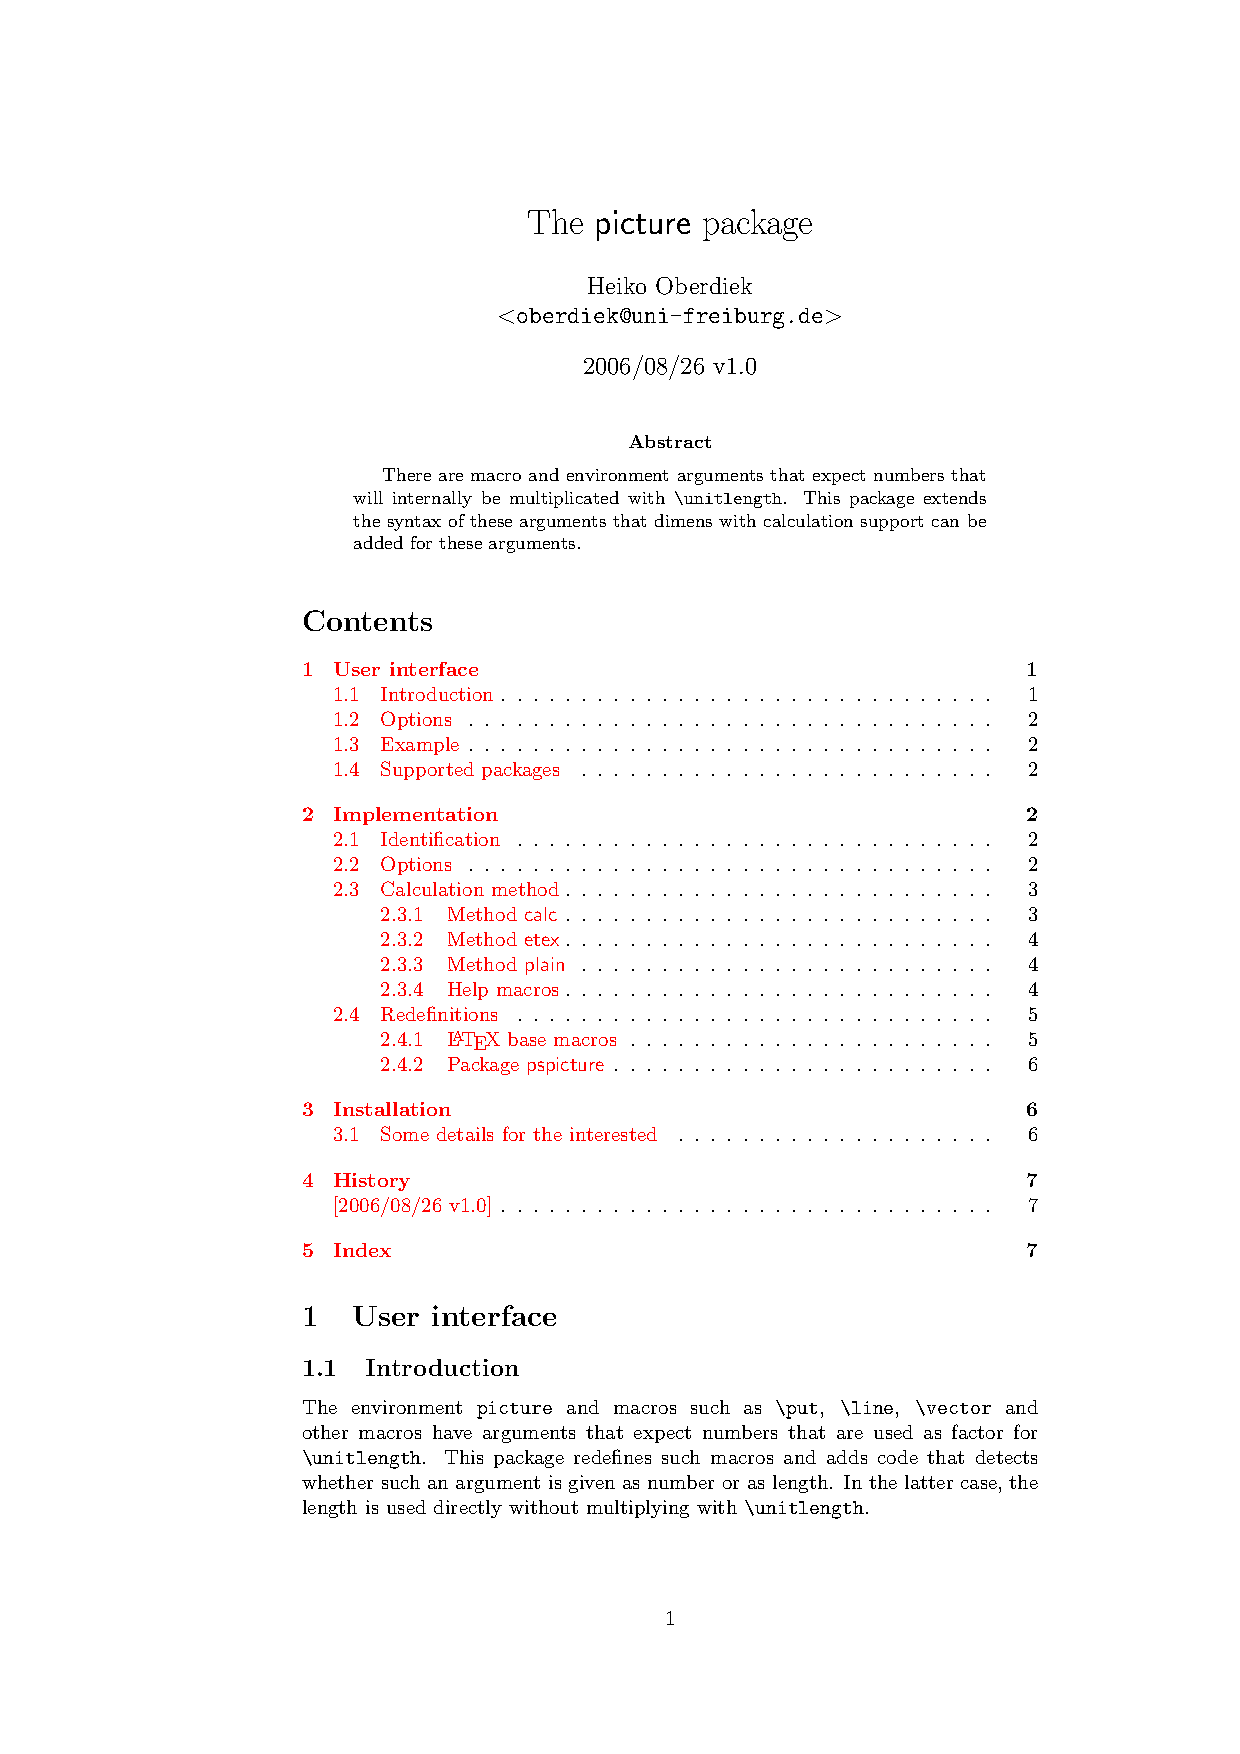
\includegraphics{picture}
\input{explanation}
\end{verbatim}
\end{quote}
then \cmdinvoke{import}{/home/friend/}{results} will include both
graph and explanation as one might hope.  A \csx{subimport} command
does the same sort of thing for a subdirectory (a relative path rather
than an absolute one), and there are corresponding \csx{includefrom}
and \csx{subincludefrom} commands.

The \Package{chapterfolder} package provides commands to deal with its
(fixed) model of file inclusion in a document.  It provides commands
\csx{cfpart}, \csx{cfchapter}, \csx{cfsection} and \csx{cfsubsection},
each of which takes directory and file arguments, e.g.:
\begin{quote}
\begin{verbatim}
\cfpart[pt 1]{Part One}{part1}{part}
\end{verbatim}
\end{quote}
which command will issue a `normal' command % ! line break
\cmdinvoke{part}[pt 1]{Part One} and then input the file
\File{part1/part.tex}, remembering that \File{part1/} is now the
``current folder''.  There are also commands of the form
\csx{cfpartstar} (which corresponds to a \csx{part*} command).

Once you're ``in'' a \Package{chapterfolder}-included document, you
may use \csx{cfinput} to input something relative to the ``current
folder'', or you may use \csx{input}, using \csx{cfcurrentfolder} to
provide a path to the file.  (There are also
\csx{cfcurrentfolderfigure} for a \path{figure/} subdirectory and
\csx{cfcurrentfolderlistings} for a \path{listings/} subdirectory.)

Documentation of \Package{chapterfolder} is in French, but the
\File{README} in the directory is in English.
\begin{ctanrefs}
\item[chapterfolder.sty]\CTANref{chapterfolder}
\item[import.sty]\CTANref{import}
\end{ctanrefs}

\Question[Q-RCS]{Version control using \acro{RCS}, \acro{CVS} or \ProgName{Subversion}}

If you use \acro{RCS}, \acro{CVS} or \ProgName{Subversion} to maintain
your \AllTeX{} documents under version control, you may need some
mechanism for including the version details in your document, in such
a way that they can be typeset (that is, rather than just hiding them
inside a comment).

The most complete solution for \acro{RCS} and \acro{CVS} is to use the
(\LaTeX{}) package \Package{rcs}, which allows you to parse and
display the contents of \acro{RCS} keyword fields in an extremely
flexible way.  The package \Package{rcsinfo} is simpler, but does most
of what you want, and some people prefer it; it is explicitly
compatible with \ProgName{LaTeX2HTML}.

If, however, you need a solution which works without using external
packages, or which will work in Plain \TeX{}, then you can use the
following minimal solution:
\begin{quote}
\begin{wideversion}
\begin{verbatim}
\def\RCS$#1: #2 ${\expandafter\def\csname RCS#1\endcsname{#2}}
\RCS$Revision: 1.426 $ % or any RCS keyword
\RCS$Date: 2006/12/18 09:59:16 $
...
\date{Revision \RCSRevision, \RCSDate}
\end{verbatim}
\end{wideversion}
\begin{narrowversion}
\begin{verbatim}
\def\RCS$#1: #2 ${\expandafter
  \def\csname RCS#1\endcsname{#2}%
}
\RCS$Revision: 1.426 $ % or any RCS keyword
\RCS$Date: 2006/12/18 09:59:16 $
...
\date{Revision \RCSRevision, \RCSDate}
\end{verbatim}
\end{narrowversion}
\end{quote}

If you've entered the brave new world of \ProgName{subversion}, the
package \Package{svn} may be for you.  It has explicit cleverness
about dealing with dates:
\begin{quote}
\csx{documentclass}\texttt{\{\meta{foo}\}}\\
\texttt{...}\\
\cmdinvoke{usepackage}{svn}\\
\csx{SVNdate}\texttt{ \$Date\$}\\
\cmdinvoke{author}{...}\\
\cmdinvoke{title}{...}\\
\texttt{...}\\
\cmdinvoke{begin}{document}\\
\csx{maketitle}\\
\texttt{...}\\
\cmdinvoke{end}{document}
\end{quote}
will (once \ProgName{subversion} has committed a copy of the document)
cause \csx{maketitle} use the date that has been written into the
\texttt{\$Date\$} keyword.

The alternative is the \Package{svninfo} package, which has much the
same mechanisms as does \Package{svn} but with a rather different
focus.  \Package{Svninfo} does the date trick that \Package{svn}
performs (controlled by a package option), and can set up page
foot-lines using \Qref*{package \Package{fancyhdr}}{Q-fancyhdr}.
There isn't much to choose between the two packages: you should read
the packages' documentation to see which you find best.
\begin{ctanrefs}
\item[rcs.sty]\CTANref{rcs}
\item[rcsinfo.sty]\CTANref{rcsinfo}
\item[svn.sty]\CTANref{svn}
\item[svninfo.sty]\CTANref{svninfo}
\end{ctanrefs}

\Question[Q-make]{Makefiles for \LaTeX{} documents}

\LaTeX{} is a tricky beast for running \ProgName{make} on: the need to
instruct \LaTeX{} to run several times for essentially different
reasons (for example, ``get the table of contents stable'', ``get the
labels stable'', ``add the bibliography'', ``add the index'') is
actually rather difficult to express in the `ordinary' sort of
dependency graph that one constructs for \ProgName{make}.

For this reason, the only \ProgName{make}-like package on \acro{CTAN}
(for a long time) was \ProgName{latexmk}, which is a \ProgName{Perl}
script that analyses your \LaTeX{} source for its dependencies, runs
\BibTeX{} or \ProgName{makeindex} as and when it notices that those
programs' input (parts of the |.aux| file, or the |.idx| file,
respectively) has changed, and so on.  \ProgName{Latexmk} is a fine
solution (and was used in generating printable versions of these
\acro{FAQ}s for a long time); it has recently been upgraded and has
many bells and whistles that allow it to operate as if it were a poor
man's \WYSIWYG{} system.

The \Qref*{\Package{texinfo} system}{Q-texinfo} comes with a
utility called \ProgName{texi2dvi}, which is capable of ``converting''
either \LaTeX{} or \Package{texinfo} files into \acro{DVI} (or into
\acro{PDF}, using \PDFTeX{}).

A later contribution is the bundle \Package{latexmake}, which
offers a set of \ProgName{make} rules that invoke \ProgName{texi2dvi}
as necessary.

The curious may examine the rules employed to run the present
\acro{FAQ} through \LaTeX{}: we don't present them as a complete
solution, but some of the tricks employed are surely re-usable.
\begin{ctanrefs}
\item[\nothtml{\rmfamily}\acro{FAQ} distribution]\CTANref{faq}
\item[\nothtml{\rmfamily}latexmake]\CTANref{latexmake}
\item[latexmk]\CTANref{latexmk}
\item[texi2dvi]Distributed as part of \CTANref{texinfo}
\end{ctanrefs}

\Question[Q-howmanypp]{How many pages are there in my document?}

Simple documents (those that start at page 1, and don't have any
breaks in their page numbering until their last page) present no
problem to the seeker after this truth.  The number of pages is
reported by the \Package{lastpage} package in its \texttt{LastPage} label.

For more complicated documents (most obviously, books with frontmatter
in a different series of page numbers) this simple approach will not
do.

The \Package{count1to} package defines a label \texttt{TotalPages}; this is
the value of its copy of \csx{count1} (a reserved \TeX{} count
register) at the end of the document.

Package \Package{totpages} defines a label \texttt{TotPages}, but it also
makes the register it uses available as a \LaTeX{} counter,
\texttt{TotPages}, which you can also reference via \csx{theTotPages}.  Of
course, the counter |TotPages| is asynchronous in the same way that
page numbers are, but snapshots may safely be taken in the output
routine.

The \Class{memoir} class defines two counters \texttt{lastpage} and
\texttt{lastsheet}, which are set (after the first run of a document)
to the equivalent of the \texttt{LastPage} label and the
\texttt{TotalPages} labels.

Both \Package{count1to} and \Package{totpages} need the support of
the \Package{everyshi} package.
\begin{ctanrefs}
\item[count1to.sty \nothtml{\bgroup\rmfamily}and\nothtml{\egroup} everyshi.sty]% line break!!
  Distributed in \CTANref{ms}
\item[lastpage.sty]\CTANref{lastpage}
\item[memoir.cls]\CTANref{memoir}
\item[totpages.sty]\CTANref{totpages}
\end{ctanrefs}

\Question[Q-inclplain]{Including Plain \TeX{} files in \LaTeX{}}

\LaTeX{}, though originally \nothtml{based on Plain \TeX{} (}% beware line brk
\Qref{based on Plain \TeX{}}{Q-LaTeXandPlain}\nothtml{)}, does not
contain all of Plain \TeX{}'s commands.  Worse, some Plain \TeX{}
command names appear in \LaTeX{}, with different semantics.  As a
result, special measures need to be taken to allow general Plain
\TeX{} documents (or parts of documents) to be typeset within
\LaTeX{}.

The truly reliable way is to translate the Plain \TeX{} commands, to
produce an equivalent of the original's semantics.  However, this is
not practical in many circumstances, and for those occasions, the
\Package{plain} package will often come to your aid.  The package
defines a \environment{plain} environment, in which a Plain \TeX{}
document may be processed:
\begin{quote}
\begin{verbatim}
\begin{plain}
  \input{plain-doc}
\end{plain}
\end{verbatim}
\end{quote}
The package is known to fail, for example, with documents that use
\AMSTeX{}; no doubt it would also fail if asked to load \Eplain{}.
All these things can be overcome (although it's not often easy), but
the environment saves a lot of work on many occasions.
\begin{ctanrefs}
\item[plain.sty]Distributed as part of \CTANref{carlisle}
\end{ctanrefs}

\subsection{Hyphenation}

\Question[Q-nohyph]{My words aren't being hyphenated}

Let's assume you've selected the right \TeX{} `language'~--- as
explained in \Qref[question]{``how hyphenation works''}{Q-hyphen},
you're not likely to get the correct results typesetting one language
using the hyphenation rules of another.  (Select the proper language,
using \Package{babel} if you're a \LaTeX{} user.  This may reveal that
you need another set of hyphenation patterns; see
% beware line wrap
\Qref[question]{``using a new language''}{Q-newlang} for advice on how
to install it.)

So what else can go wrong?
\begin{itemize}
\item Since \TeX{} version~3.0, the limits on how near to either end
  of a word hyphenation may take place have been programmable (see
  \Qref[question]{``weird hyphenation''}{Q-weirdhyphen}), and for some
  reason the values in question may have been corrupted in some macros
  you are using.  \TeX{} won't hyphenate less than \csx{lefthyphenmin}
  characters after the start of a word, nor less than
  \csx{righthyphenmin} before the end of a word; thus it won't
  hyphenate a word shorter than the sum of the two minima, at all.
  For example, since the minima are 2 and 3 for English, \TeX{} won't
  hyphenate a word shorter than 5 letters long, if it believes the
  word to be English.
\item \TeX{} won't hyphenate a word that's already been hyphenated.
  For example, the (caricature) English surname Smyth-Postlethwaite
  wouldn't hyphenate, which could be troublesome.  This is correct
  English typesetting style (it may not be correct for other
  languages), but if needs must, you can replace the hyphen in the
  name with a \csx{hyph} command, defined
\begin{quote}
\begin{verbatim}
\def\hyph{-\penalty0\hskip0pt\relax}
\end{verbatim}
\end{quote}
  This is \emph{not} the sort of thing this \acro{FAQ} would
  ordinarily recommend\dots{} The \Package{hyphenat} package defines a
  bundle of such commands (for introducing hyphenation points at
  various punctuation characters).
\item There may be accents in the word.  The causes of and remedies
  for this effect are discussed in
  % beware line break
  \Qref[question]{accents and hyphens}{Q-hyphenaccents}.
\item The hyphenation may simply not have been spotted; while \TeX{}'s
  algorithm is good, it's not infallible, and it does miss perfectly
  good hyphenations in some languages.  When this happens, you need to
  give \TeX{} \emph{explicit} instructions on how to hyphenate.
\end{itemize}
The \csx{hyphenation} command allows you to give explicit instructions.
Provided that the word will hyphenate at all (that is, it is not
prevented from hyphenating by any of the other restrictions above),
the command will override anything the hyphenation patterns might
dictate.  The command takes one or more hyphenated words as
argument~--- \cmdinvoke{hyphenation}{ana-lysis pot-able}; note that
(as here, for analysis) you can use the command to overrule \TeX{}'s
choice of hyphenation (ana-lysis is the British etymological
hyphenation; some feel the American hyphenation feels
`unfortunate'\dots{}).
\begin{ctanrefs}
\item[hyphenat.sty]\CTANref{hyphenat}
\end{ctanrefs}

\Question[Q-weirdhyphen]{Weird hyphenation of words}

If your words are being h-yphenated, like this, with jus-t single
letters at the 
beginning or the end of the word, you may have a version mismatch
problem. \TeX{}'s hyphenation system changed between version~2.9
and~3.0, and macros written for use with version~2.9 can have this
effect with a version~3.0 system.  If you are using Plain \TeX{}, make
sure your \File{plain.tex} file has a version number which is at
least~3.0, and rebuild your format.  If you are using \LaTeXo{} your
best plan is to upgrade to \LaTeXe{}.  If for some reason you can't,
the last version of \LaTeXo{} (released on 25 March 1992) is still
available (for the time being at least) and ought to solve this
problem.

If you're using \LaTeXe{}, the problem probably arises from your
|hyphen.cfg| file, which has to be created if you're using a
multi-lingual version.

A further source of oddity can derive from the 1995 release of
\Qref*{Cork-encoded fonts}{Q-ECfonts},
which introduced an alternative hyphen character.  The \LaTeXe{}
configuration files in the font release specified use of the
alternative hyphen, and this could produce odd effects with words
containing an explicit hyphen.  The font configuration files in the
December 1995 release of \LaTeXe{} do \emph{not} use the alternative
hyphen character, and therefore removed this source of problems; the
solution, again, is to upgrade your \LaTeX{}.
\begin{ctanrefs}
\item[\nothtml{\rmfamily}\LaTeXo{}]\CTANref{latex209-base}
\item[plain.tex]\CTANref{plain}
\end{ctanrefs}

\Question[Q-oddhyphen]{(Merely) peculiar hyphenation}

You may have found that \TeX{}'s famed automatic word-division does
not produce the break-points recommended by your dictionary. This may be
because \TeX{} is set up for American English, whose rules for word
division (as specified, for example, in Webster's Dictionary) are
completely different from the British ones (as specified, for example,
in the Oxford Dictionaries). This problem is being addressed by the \acro{UK}
\TeX{} User community (see \BV{}, issue~4.4) but an entirely
satisfactory solution will take time; the current status is to be
found on \acro{CTAN} (see
% beware line-wrap
\Qref[question]{``using a new language''}{Q-newlang} for instructions
on adding this new ``language'').
\begin{ctanrefs}
\item[UK patterns]\CTANref{ukhyph}
\end{ctanrefs}

\Question[Q-hyphenaccents]{Accented words aren't hyphenated}

\TeX{}'s algorithm for hyphenation gives up when it encounters an
\csx{accent} command; there are good reasons for this, but it means
that quality typesetting in non-English languages can be difficult.

For \TeX{} macro packages, you can avoiding the effect by using an
appropriately encoded font (for example, a Cork-encoded font~--- see
\Qref[question]{the \acro{EC} fonts}{Q-ECfonts}) which contains accented
letters as single glyphs.  \LaTeX{} users can achieve this end simply
by adding the command
\begin{verbatim}
  \usepackage[T1]{fontenc}
\end{verbatim}
to the preamble of their document.  Other encodings (notably
\acro{LY}1, once promoted by \YandY{} inc) may be used
in place of \acro{T}1.  Indeed, most current 8-bit \TeX{} font
encodings will `work' with the relevant sets of hyphenation patterns. 

One might hope that, with the many aspirant successors to \TeX{} such
as
\begin{wideversion}
  \Qref{Omega}{Q-omegaleph}, \Qref{\acro{LUA}\TeX{}}{Q-luatex} and
  \Qref{Ex\TeX{}}{Q-extex},
\end{wideversion}
\begin{narrowversion}
  Omega, \acro{LUA}\TeX{} and Ex\TeX{}
  (\Qref[see questions]{}{Q-omegaleph}\Qref[,]{}{Q-luatex}
  \Qref[and]{}{Q-extex}),
\end{narrowversion}
all of which base their operations on Unicode, that the whole basis of
encodings will change.

\Question[Q-newlang]{Using a new language with Babel}

\Package{Babel} is capable of working with a large range of
languages, and a new user often wants to use a language that her
\TeX{} installation is not set up to employ.  Simply asking Babel to
use the language, with the command
\begin{verbatim}
  \usepackage[catalan]{babel}
\end{verbatim}
provokes the warning message
\begin{wideversion}
\begin{verbatim}
Package babel Warning: No hyphenation patterns were loaded for
(babel)                the language `Catalan'
(babel)                I will use the patterns loaded for \language=0 instead.
\end{verbatim}
\end{wideversion}
\begin{narrowversion}
\begin{verbatim}
Package babel Warning: No hyphenation patterns
                                 were loaded for
(babel)                the language `Catalan'
(babel)                I will use the patterns
                 loaded for \language=0 instead.
\end{verbatim}
(The first and third lines above have been wrapped to fit in the
column.)
\end{narrowversion}

The problem is that your \TeX{} system doesn't know how to hyphenate
Catalan text: you need to tell it how before Babel can do its work
properly.  To do this, for \LaTeX{} installations, one needs to change
\File{language.dat} (which is part of the Babel installation); it will
contain a line
\begin{verbatim}
%catalan         cahyphen.tex
\end{verbatim}
which, if you remove the comment marker, is supposed to instruct
\LaTeX{} to load Catalan hyphenation patterns when you tell it to build
a new format.

Unfortunately, in many Babel distributions, the line just isn't
right~--- you need to check the name of the file containing the
patterns you're going to use.  As you can see, in the author's system,
the name is supposed to be \File{cahyphen.tex}; however the file
actually present on the system is \File{cahyph.tex}~--- fortunately,
the error should prove little more than an inconvenience (most of the
files are in better distributions anyway, but an elusive one
may be found on \acro{CTAN}; if you have to retrieve
a new file, ensure that it's correctly installed, for which see
\Qref[question]{installing a new package}{Q-instpackages}).

Finally, you need to regenerate the formats used (in fact, most users
of Babel are using it in their \LaTeX{} documents, so regenerating the
\LaTeX{}-related formats will ordinarily be enough; however, the
author always generates the lot, regardless).
\begin{description}
\item[te\TeX{}]It's possible to do the whole operation in one go, by
  using the \ProgName{texconfig} command:
\begin{verbatim}
texconfig hyphen latex
\end{verbatim}
  which first enters an editor for you to edit \File{language.dat},
  and then regenerates the format you specify (\ProgName{latex} in
  this case).

  Otherwise, to regenerate all formats, do: \\
  \texttt{fmtutil -\relax-all}
  
  If you're willing to think through what you're doing (this is
  \emph{not} for the faint-hearted), you can select a sequence of
  formats and for each one, run: \\
  \texttt{fmtutil -\relax-byfmt \meta{formatname}}\\
  where \emph{\texttt{formatname}} is something like `\texttt{latex}',
  or: \\
  \texttt{fmtutil -\relax-byhyphen \meta{hyphenfile}}\\
  where \emph{\texttt{hyphenfile}} is the file specifying hyphenation
  to the format~--- usually \texttt{language.dat}
\item[\miktex{}] On a \Package{\miktex{}} distribution earlier than v2.0, do: \\
  \texttt{Start}\arrowhyph{}%
  \texttt{Programs}\arrowhyph{}%
  \texttt{\miktex{}}\arrowhyph{}%
  \texttt{Maintenance}\arrowhyph{}%
  \texttt{Create all format files}
% this sequence suggested for miktex 1.20e, 2000/12/22, by Giuseppe Bilotta

  or get a DOS window and run:\\
  \texttt{initexmf -\relax-dump}
  
  On a \Package{\miktex{}} distribtution v2.0 or later, the whole
  procedure can be done via the \acro{GUI}.  To select the new
  language, do:\\
  \texttt{Start}\arrowhyph{}%
  \texttt{Programs}\arrowhyph{}%
  \texttt{\miktex{} 2}\arrowhyph{}%
  \texttt{\miktex{} Options}, and select the \texttt{Languages} tab.
  Select your language from the list, press the \texttt{Apply} button,
  and then the \texttt{OK} button.  Then select the \texttt{General}
  tab and press the \texttt{Update Now} button.
  
  Otherwise, edit the \File{language.dat} file (as outlined above),
  and then run:\\
  \texttt{initexmf -\relax-dump}\\
  just as for a pre-v2.0 system.
\end{description}

\nothtml{\noindent}\textbf{\emph{Caveat}:} It is (just) possible that
your \TeX{} system may run out of ``pattern memory'' while generating
the new format.  Most \TeX{} implementations have fixed-size arrays
for storing the details of hyphenation patterns, but although their
size is adjustable in most modern distributions, actually changing the
size is a fiddle.  If you \emph{do} find you've run out of memory,
it may be worth scanning the list of languages in your
\File{language.dat} to see whether any could reasonably be removed.
\begin{ctanrefs}
\item[babel]\CTANref{babel}
\item[hyphenation patterns]\CTANref{hyphenation}
\end{ctanrefs}

\Question[Q-hyphoff]{Stopping all hyphenation}

It may seem an odd thing to want to do (after all, one of \TeX{}'s
great advertised virtues is the quality of its hyphenation) but it's
sometimes necessary.  The real problem is, that the quality of
\TeX{}'s output is by default largely dependent on the presence of
hyphenation; if you want to abandon hyphenation, something has to
give.

\TeX{} (slightly confusingly) offers four possible mechanisms for
suppressing hyphenation (there were only two prior to the extensions
that arrived with \TeX{} version~3).

First, one can set the hyphenation penalties \csx{hyphenpenalty} and
\csx{exhyphenpenalty} to an `infinite' value (that is to say, 10000).
This means that all hyphenations will sufficiently penalise the line
that would contain them, that the hyphenation won't happen.  The
disadvantage of this method is that \TeX{} will re-evaluate any
paragraph for which hyphenations might help, which will slow \TeX{}
down.

Second, one can select a language for which no hyphenation patterns
exist.  Some distributions create a language |nohyphenation|,
and the \Package{hyphenat} package uses this technique for its
\csx{nohyphens} command which sets its argument without any
hyphenation.

Third, one can set \csx{left-} and/or \csx{righthyphenmin} to a
sufficiently large value that no hyphenation could possibly succeed,
since the minimum is larger than the length of the longest word
\TeX{} is willing to hyphenate (the appropriate value is 62).

Fourth, one can suppress hyphenation for all text using the current
font by the command
\begin{quote}
\begin{verbatim}
\hyphenchar\font=-1
\end{verbatim}
\end{quote}
This isn't a particularly practical way for users to suppress
hyphenation~--- the command has to be issued for every font the
document uses~--- but it's how \LaTeX{} itself suppresses hyphenation
in \texttt{tt} and other fixed-width fonts.

Which of the techniques you should use depends on what you actually
want to do.  If the text whose hyphenation is to be suppressed runs
for less than a paragraph, your only choice is the no-hyphens
language: the language value is preserved along with the text (in the
same way that the current font is); the values for penalties and
hyphen minima active at the end of a paragraph are used when
hyphenation is calculated.

Contrariwise, if you are writing a multilanguage document using the
\Package{babel} package, you \emph{cannot} suppress hyphenation
throughout using either the no-hyphens language or the hyphen minima:
all those values get changed at a \Package{babel} language switch: use
the penalties instead.

If you simply switch off hyphenation for a good bit of text, the
output will have a jagged edge (with many lines seriously overfull),
and your \AllTeX{} run will bombard you with warnings about overfull
and underfull lines.  To avoid this you have two options.  You may use
\csx{sloppy} (or its environment version \environment{sloppypar}), and
have \TeX{} stretch what would otherwise be underfull lines to fill the space
offered, and wrap other lines, while prematurely wrapping overfull
lines and stretching the remainder.  Alternatively, you may set the
text \Qref*{ragged right}{Q-ragright}, and at least get rid of
the overfull lines; this technique is `traditional' (in the sense that
typists do it) and may be expected to appeal to the specifiers of
eccentric document layouts (such as those for dissertations), but for
once their sense conforms with typographic style.  (Or at least, style
constrained in this curious way.)
\begin{ctanrefs}
\item[hyphenat.sty]\CTANref{hyphenat}
\end{ctanrefs}

\Question[Q-wdnohyph]{Preventing hyphenation of a particular word}

It's quite possible for (\emph{any}) hyphenation of a particular word
to seem ``completely wrong'', so that you want to prevent it being
hyphenated.

If the word occurs in just one place, put it in a box:
\begin{quote}
\begin{verbatim}
\mbox{oddword}
\end{verbatim}
\end{quote}
(Plain~\TeX{} users should use \csx{hbox}, and take care at the start
of paragraphs.)  However, boxing the word is not really advisable
unless you are sure it only occurs once.

If the word occurs commonly, the best choice is to assert a
non-hyphenation for it:
\begin{quote}
\begin{verbatim}
\hyphenation{oddword}
\end{verbatim}
\end{quote}
This hyphenation exception (with no break points) will be used in
preference to what \TeX{}'s hyphenation algorithm may come up with.

In a multilingual document, repeat the exception specification for
each language the word may appear in.  So:
\begin{quote}
\begin{verbatim}
\usepackage[french,english]{babel}
\selectlanguage{english}
\hyphenation{oddword}
\selectlanguage{french}
\hyphenation{oddword}
\end{verbatim}
\end{quote}
(note that \Package{babel} will select the default language for the
document~--- English, in this case~--- at \cmdinvoke{begin}{document}.)

\Question[Q-hyphexcept]{Hyphenation exceptions}

While \TeX{}'s hyphenation rules are good, they're not infallible: you
will occasionally find words \TeX{} just gets \emph{wrong}.  So for
example, \TeX{}'s default hyphenation rules (for American English) don't
know the word ``\emph{manuscript}'', and since it's a long word you
may find you need to hyphenate it.  You \emph{can} ``write the
hyphenation out'' each time you use the word:
\begin{quote}
\begin{verbatim}
... man\-u\-script ...
\end{verbatim}
\end{quote}
Here, each of the \csx{-} commands is converted to a hyphenated break,
if (\emph{and only if}) necessary.

That technique can rapidly become tedious: you'll probably only accept
it if there are no more than one or two wrongly-hyphenated words in
your document.  The alternative is to set up hyphenations in the
document preamble.  To do that, for the hyphenation above, you would
write:
\begin{quote}
\begin{verbatim}
\hyphenation{man-u-script}
\end{verbatim}
\end{quote}
and the hyphenation would be set for the whole document.  Barbara
Beeton publishes articles containing lists of these ``hyphenation
exceptions'', in \textsl{TUGboat}; the hyphenation `man-u-script'
comes from one of those articles.

What if you have more than one language in your document?  Simple:
select the appropriate language, and do the same as above:
\begin{quote}
\begin{verbatim}
\usepackage[french]{babel}
\selectlanguage{french}
\hyphenation{re-cher-cher}
\end{verbatim}
\end{quote}
(nothing clever here: this is the ``correct'' hyphenation of the word,
in the current tables).  However, there's a problem here: just as
words with accents in them won't break, so \csx{hyphenation} commands
with accents in them produce an error:
\begin{quote}
\begin{verbatim}
\usepackage[french]{babel}
\selectlanguage{french}
\hyphenation{r\'e-f\'e-rence}
\end{verbatim}
\end{quote}
tells us that the hyphenation is ``improper'', and that it will be ``flushed''.
But, just as hyphenation of words is enabled by selecting an 8-bit
font encoding, so \csx{hyphenation} commands are rendered proper again
by selecting that same 8-bit font encoding.  For the hyphenation
patterns provided in the usual distributions, the encoding is
\Qref*{Cork}{Q-ECfonts}, so the complete sequence is:
\begin{quote}
\begin{verbatim}
\usepackage[T1]{fontenc}
\usepackage[french]{babel}
\selectlanguage{french}
\hyphenation{r\'e-f\'e-rence}
\end{verbatim}
\end{quote}

The same sort of performance goes for any language for which 8-bit
fonts and corresponding hyphenation patterns are available.  Since you
have to select both the language and the font encoding to have your
document typeset correctly, it should not be a great imposition to do
the selections before setting up hyphenation exceptions.

\subsection{Odds and ends}

\Question[Q-logos]{Typesetting all those \TeX{}-related logos}

Knuth was making a particular point about the capabilities of \TeX{}
when he defined the logo.  Unfortunately, many believe, he thereby
opened floodgates to give the world a whole range of rather silly
`bumpy road' logos such as \AMSTeX{}, \PiCTeX{}, \BibTeX{}, and so on,
produced in a flurry of different fonts, sizes, and baselines~--- indeed,
everything one might hope to cause them to obstruct the reading process.
In particular, Lamport invented \LaTeX{}
\htmlignore
(silly enough in itself)
\endhtmlignore
\begin{htmlversion}
  (silly enough in itself, with a raised small `A' and a lowered `E')
\end{htmlversion}
and marketing input from Addison-Wesley led to the even
stranger current logo
\htmlignore
\LaTeXe{}.
\endhtmlignore
\begin{htmlversion}
  \LaTeXe{}, which appends a lowered single-stroke Greek letter
  epsilon.
\end{htmlversion}

Sensible users don't have to follow this stuff wherever it goes,
but, for those who insist, a large collection of logos is defined in
the \Package{texnames} package (but note that this set of macros isn't
entirely reliable in \LaTeXe{}).
The \MF{} and \MP{} logos can be set in fonts that \LaTeXe{}
knows about (so that they scale with the surrounding text) using the
\Package{mflogo} package; but be aware that booby-traps surround the
use of the Knuthian font for \MP{} (you might get
\htmlignore
\textlogo{META\hphantom{P}O\hphantom{S}T}).
\endhtmlignore
% the following htmlversion stuff seems to do roughly what's required,
% which is nice, given the feebleness of representing all these silly
% logos in html otherwise...
\begin{htmlversion}
  something like `META&nbsp;O&nbsp;T').
\end{htmlversion}
You needn't despair, however~--- the author himself uses just `MetaPost'.

For those who don't wish to acquire the `proper' logos, the canonical
thing to do is to say \texttt{AMS-}\cmdinvoke{TeX}{}
\htmlignore
(\acro{AMS}-\TeX{})
\endhtmlignore
for \AMSTeX{}, \texttt{Pic}\cmdinvoke{TeX}{}
\htmlignore
(Pic\TeX{})
\endhtmlignore
for \PiCTeX{}, \texttt{Bib}\cmdinvoke{TeX}{}
\htmlignore
(Bib\TeX{})
\endhtmlignore
for \BibTeX{}, and so on.
\begin{ctanrefs}
\item[mflogo.sty]\CTANref{mflogo}
\item[texnames.sty]\CTANref{texnames}
\end{ctanrefs}

\Question[Q-bold-extras]{How to do bold-tt or bold-sc}

\LaTeX{}, as delivered, offers no means of handling bold ``teletype''
or small-caps fonts.  There's a practical reason for this (Knuth never
designed such fonts), but there are typographical considerations too
(the ``medium weight'' \texttt{cmtt} font is already pretty bold (by
comparison with other fixed-width fonts), and bold small-caps is not
popular with many professional typographers).

There's a set of ``extra'' \MF{} files on \acro{CTAN} that provide bold
versions of both \texttt{cmtt} and \texttt{cmcsc} (the small caps font).  With
modern \TeX{} distributions, one may bring these fonts into use simply
by placing them in an % ! line break
\Qref*{appropriate place in the \emph{texmf} tree}{Q-wherefiles}
(these are \AllTeX{}-specific files, so the ``\emph{public}'' supplier
would be an appropriate place).  Once you've % ! line break, again
\Qref*{rebuilt the file indexes as necessary}{Q-instpackages},
\TeX{} (and friends) will automatically build whatever font files they
need when you first make reference to them.  There's a jiffy package
\Package{bold-extra} that builds the necessary font data structures
so that you can use the fonts within \LaTeX{}.

Another alternative is to use the \Qref*{\acro{EC} fonts}{Q-ECfonts},
which come with bold variants of the small-caps fonts.

If you need to use Type~1 fonts, you can't proceed with Knuth-style
fonts, since there are no Type~1 versions of the \Package{mf-extra}
set.  There are, however, Type~1 distributions of the EC~fonts, so you
can switch to EC and use them; alternatives are discussed in
\Qref[question]{8-bit Type~1 fonts}{Q-type1T1}.

Of course, commercial fixed-width fonts (even the default
\FontName{Courier}) almost always come with a bold variant, so that's
not a problem.  Furthermore \Qref*{\acro{PSNFSS}}{Q-usepsfont}
will usually provide ``faked'' small caps fonts, and has no
compunctions about providing them in a bold form.  \FontName{Courier}
is (as we all know, to our cost) freely available; a far more
presentable monospace font is \FontName{LuxiMono}, which is also
freely available (monospace text in the typeset version of this
\acro{FAQ} uses \FontName{LuxiMono}, with the metrics and \LaTeX{}
support available on the archive.
\begin{ctanrefs}
\item[bold-extra.sty]\CTANref{bold-extra}
\item[bold tt and small caps fonts]\CTANref{bold}
\item[\nothtml{rmfamily}LuxiMono fonts]\CTANref{luximono}
\end{ctanrefs}

\Question[Q-varwidth]{Automatic sizing of \environment{minipage}}

The \environment{minipage} environment requires you to specify the
width of the ``page'' you're going to create.  This is sometimes
inconvenient: you would like to occupy less space, if possible, but
\environment{minipage} sets a box that is exactly the width you
specified.

The \Package{pbox} package defines a \csx{pbox} whose width is exactly
that of the longest enclosed line, subject to a maximum width that you
give it.  So while \cmdinvoke{parbox}{2cm}{Hello\bsbs world!} produces a
box of width exactly \texttt{2cm},
\cmdinvoke{pbox}{2cm}{Hello\bsbs world!} produces one whose width is
\texttt{1.79cm} (if one's using the default \FontName{cmr} font for the
text, at least).  The package also provides a
\cmdinvoke*{settominwidth}[min]{length}{text} (which looks (almost)
like the standard \csx{settowidth} command), and a \csx{widthofpbox}
function analagous to the \csx{widthof} command for use with the
\Package{calc} package.

The \Package{eqparbox} package extends \Package{pbox}'s idea, by
allowing you to set a series of boxes, all with the same (minimised)
width.  (Note that it doesn't accept a limiting maximum width
parameter.)  The package documentation shows the following example
drawn from a joke \emph{curriculum vitae}:
\begin{quote}
\begin{narrowversion}
\begin{verbatim}
\noindent%
\eqparbox{place}%
    {\textbf{Widgets, Inc.}}
        \hfill
\eqparbox{title}%
    {\textbf{Senior Widget Designer}}
        \hfill
\eqparbox{dates}{\textbf{1/95--present}}

...

\noindent%
\eqparbox{place}%
    {\textbf{Thingamabobs, Ltd.}}
        \hfill
\eqparbox{title}%
    {\textbf{Lead Engineer}}
        \hfill
\eqparbox{dates}{\textbf{9/92--12/94}}
\end{verbatim}
\end{narrowversion}
\begin{wideversion}
\begin{verbatim}
\noindent%
\eqparbox{place}{\textbf{Widgets, Inc.}} \hfill
\eqparbox{title}{\textbf{Senior Widget Designer}} \hfill
\eqparbox{dates}{\textbf{1/95--present}}

...

\noindent%
\eqparbox{place}{\textbf{Thingamabobs, Ltd.}} \hfill
\eqparbox{title}{\textbf{Lead Engineer}} \hfill
\eqparbox{dates}{\textbf{9/92--12/94}}
\end{verbatim}
\end{wideversion}
\end{quote}
The code makes the three items on each of the heading lines have
exactly the same width, so that the lines as a whole produce a regular
pattern down the page.  A command \csx{eqboxwidth} allows you to use
the measured width of a group: the documentation shows how the command
may be used to produce sensible-looking columns that mix \texttt{c}-,
\texttt{r}- or \texttt{l}-rows, with the equivalent of a |p{...}|
entry, by making the fixed-width rows an \Package{eqparbox} group, and
making the last from a \csx{parbox} using the width that's been
measured for the group.

The \Package{varwidth} package defines a \environment{varwidth}
environment which sets the content of the box to match a ``narrower
natural width'' if it finds one.  (You give it the same parameters as
you would give \environment{minipage}: in effect, it is a `drop-in'
replacement.)  \Package{Varwidth} provides its own ragged text command:
\csx{narrowragged}, which aims to make narrower lines and to put more
text in the last line of the paragraph (thus producing lines with more
nearly equal lengths than typically happens with \csx{raggedright}
itself).

The documentation (in the package file) lists various restrictions and
things still to be done, but the package is already proving useful for
a variety of jobs.
\begin{ctanrefs}
\item[eqparbox.sty]\CTANref{eqparbox}
\item[pbox.sty]\CTANref{pbox}
\item[varwidth.sty]\CTANref{varwidth}
\end{ctanrefs}

%%%%%%%%%%%%%%%%%%%%%%%%%%%%%%%%%%%%%%%%%%%%%%%%%%%%%%%%%%%%%%%%%

\section{Symbols, etc.}

\Question[Q-numbersets]{Symbols for the number sets}

It is a good idea to have commands such as \csx{R} for the real numbers and
other standard number sets. Traditionally these were typeset in bold.
Because, in the ordinary course of events, mathematicians do not have
access to bold chalk, they invented the special symbols that are now
often used for \csx{R}, \csx{C}, \emph{etc}.  These symbols are known
as ``blackboard bold''.  Before insisting on using them, consider
whether going back to the old system of ordinary bold might not be
acceptable (it is certainly simpler).

A set of blackboard bold capitals is available in the \acro{AMS}
\FontName{msbm} fonts (\FontName{msbm} is available at a range of
design sizes, with names such as \FontName{msbm10}). The pair of font
families (the other is called \FontName{msam}) have a large number of
mathematical symbols to supplement the ones in the standard \TeX{}
distribution, and are available in Type~1 format with most modern
distributions. Support files for using the fonts, both under
Plain~\TeX{} and \LaTeX{} (packages \Package{amssymb} and
\Package{amsfonts}), are available.  The font shape is a rather
austere sans, which many people don't like (though it captures the
essence of quickly-chalked writing rather well).

The \FontName{bbold} family is set of blackboard bold fonts written in
\MF{}.  This set offers blackboard bold forms of lower-case letters;
the font source directory also contains sources for a \LaTeX{} package
that enables use of the fonts.  The fonts are not available in Type~1 format.

The \FontName{bbm} family claims to provide
`blackboard' versions of most of the \FontName{cm} fonts~\dots{} including
the bold and bold-extended series.  Again, the fonts are designed in
\MF{} and are not available in Type~1 format.  \LaTeX{} macro support
comes from a package by Torsten Hilbrich.

The \FontName{doublestroke} family comes in just roman
and sans shapes, at a single weight, and is available both as \MF{}
sources and as Type~1; the font covers the uppercase latin letters,
lowercase `h' and 'k', and the digit `1'.

An alternative source of Type~1 fonts with blackboard bold characters
may be found in the steadily increasing set of complete families, both
commercial and free, that have been prepared for use with \AllTeX{}
(see % beware line break
\htmlonly{``}\Qref[question]{choice of outline fonts}{Q-psfchoice}\htmlonly{''}).
Of the free sets, the \FontName{txfonts} and \FontName{pxfonts} families
both come with replicas of \FontName{msam} and \FontName{msbm}
(though, as noted elsewhere, there are other reasons not to use these
fonts).  The \FontName{mathpazo} family includes a ``mathematically
significant'' choice of blackboard bold characters, and the
\FontName{fourier} fonts contain blackboard bold upper-case letters,
the digit `1', and lower-case `k'.

The ``lazy person's'' blackboard bold macros:
\begin{quote}
\begin{verbatim}
\newcommand{\R}{{\sf R\hspace*{-0.9ex}%
  \rule{0.15ex}{1.5ex}\hspace*{0.9ex}}}
\newcommand{\N}{{\sf N\hspace*{-1.0ex}%
  \rule{0.15ex}{1.3ex}\hspace*{1.0ex}}}
\newcommand{\Q}{{\sf Q\hspace*{-1.1ex}%
  \rule{0.15ex}{1.5ex}\hspace*{1.1ex}}}
\newcommand{\C}{{\sf C\hspace*{-0.9ex}%
  \rule{0.15ex}{1.3ex}\hspace*{0.9ex}}}
\end{verbatim}
\end{quote}
are almost acceptable at normal size if the surrounding text is
\FontName{cmr10}.  However, they are not part of a proper maths font,
and so do not work in sub- and superscripts.  Moreover, the size and
position of the vertical bar can be affected by the font of the
surrounding text.  As we've seen, there are plenty of alternatives:
don't try the macros, or anything similar using capital `I' (which
looks even worse!).
\begin{ctanrefs}
\item[AMS support files (Plain)]\CTANref{amsfonts-plain}
\item[AMS support files (LaTeX)]\CTANref{amsfonts-latex}
\item[AMS symbol fonts]\CTANref{amsfonts-symbols}
\item[AMS symbol fonts in Type~1 format]Browse \CTANref{ams-AMStype1}
\item[bbm fonts]\CTANref{bbm}
\item[bbm macros]\CTANref{bbm-macros}
\item[bbold fonts]\CTANref{bbold}
\item[doublestroke fonts]\CTANref{doublestroke}
\item[fourier fonts]\CTANref{fourier}
\item[mathpazo fonts]\CTANref{mathpazo}
\item[pxfonts]\CTANref{pxfonts}
\item[txfonts]\CTANref{txfonts}
\end{ctanrefs}

\Question[Q-scriptfonts]{Better script fonts for maths}

The font selected by \csx{mathcal} is the only script font `built
in'. However, there are other useful calligraphic fonts included with
modern \TeX{} distributions.
\begin{description}
\item[Euler] The \Package{eucal} package (part of most sensible \TeX{}
  distributions; the fonts are part of the \acro{AMS} font set) gives
  a slightly curlier font than the default. The package changes the
  font that is selected by \csx{mathcal}.
  
  Type 1 versions of the fonts are available in the \acro{AMS} fonts
  distribution.
\item[RSFS] The \Package{mathrsfs} package uses a really fancy script
  font (the name stands for ``Ralph Smith's Formal Script'') which is
  already part of most modern \TeX{} distributions.  The package
  creates a new command \csx{mathscr}.
  
  Type 1 versions of the font have been made available by Taco
  Hoekwater.
\item[Zapf Chancery] is the standard \PS{} calligraphic font.  There
  is no package but you can easily make it available by means of the
  command
\begin{verbatim}
\DeclareMathAlphabet{\mathscr}{OT1}{pzc}%
                                 {m}{it}
\end{verbatim}
  in your preamble.  You may find the font rather too big; if so, you
  can use a scaled version of it like this:
\begin{verbatim}
\DeclareFontFamily{OT1}{pzc}{}
\DeclareFontShape{OT1}{pzc}{m}{it}%
             {<-> s * [0.900] pzcmi7t}{}
\DeclareMathAlphabet{\mathscr}{OT1}{pzc}%
                                 {m}{it}
\end{verbatim}
  
  Adobe Zapf Chancery (which the above examples use) is distributed in
  any but the most basic \PS{} printers.  A substantially identical
  font (to the extent that the same metrics may be used) is
  available from \acro{URW} and is distributed with
  \ProgName{ghostscript}.
\end{description}
Examples of the available styles are available on \acro{CTAN}.
\begin{ctanrefs}
\item[eucal.sty]\CTANref{eucal}
\item[euler fonts]\CTANref{amsfonts-euler}
\item[euler fonts, in Type 1 format]\CTANref{ams-AMStype1}
\item[ghostscript]Browse \CTANref{ghostscript}
\item[mathrsfs.sty]Distributed as part of \CTANref{jknappen-macros}
\item[rsfs fonts]\CTANref{rsfs}
\item[rsfs fonts, in Type 1 format]\CTANref{rsfs-type1}
\item[Script font examples]\CTANref{mathscript}
\end{ctanrefs}

\Question[Q-boldgreek]{Setting bold Greek letters in \LaTeX{}}

The issue here is complicated by the fact that \csx{mathbf} (the
command for setting bold \emph{text} in \TeX{} maths) affects a select
few mathematical symbols (the uppercase Greek letters).  However
lower-case Greek letters behave differently from upper-case Greek
letters (due to Knuth's esoteric font encoding decisions).  However,
\csx{mathbf} \emph{can't} be used even for upper-case Greek letters in
the \AMSLaTeX{} \Package{amsmath} package, which
disables this font-switching and you must use one of the techniques
outlined below.

The Plain \TeX{} solution \emph{does} work, in a limited way:
\begin{quote}
\begin{verbatim}
{\boldmath$\theta$}
\end{verbatim}
\end{quote}
but \csx{boldmath} may not be used in maths mode, so this `solution'
requires arcana such as:
\begin{quote}
\begin{verbatim}
$... \mbox{\boldmath$\theta$} ...$
\end{verbatim}
\end{quote}
which then causes problems in superscripts, etc.

These problems may be addressed by using a bold mathematics package.
\begin{itemize}
\item The \Package{bm} package, which is part of the \LaTeX{} tools
  distribution, defines a command \csx{bm} which may be used anywhere
  in maths mode.
\item The \Package{amsbsy} package (which is part of \AMSLaTeX{})
  defines a command \csx{boldsymbol}, which (though slightly less
  comprehensive than \csx{bm}) covers almost all common cases.
\end{itemize}

All these solutions cover all mathematical symbols, not merely Greek
letters.
\begin{ctanrefs}
\item[bm.sty]Distributed as part of \CTANref{2etools}
\item[amsbsy.sty]Distributed as part of \AMSLaTeX{} \CTANref{amslatex}
\item[amsmath.sty]Distributed as part of \AMSLaTeX{}
  \CTANref{amslatex}
\end{ctanrefs}

\Question[Q-prinvalint]{The Principal Value Integral symbol}

This symbol (an integral sign, `crossed') does not appear in any of
the fonts ordinarily available to \AllTeX{} users, but it can be
created by use of the following macros:
\begin{wideversion}
\begin{verbatim}
\def\Xint#1{\mathchoice
   {\XXint\displaystyle\textstyle{#1}}%
   {\XXint\textstyle\scriptstyle{#1}}%
   {\XXint\scriptstyle\scriptscriptstyle{#1}}%
   {\XXint\scriptscriptstyle\scriptscriptstyle{#1}}%
   \!\int}
\def\XXint#1#2#3{{\setbox0=\hbox{$#1{#2#3}{\int}$}
     \vcenter{\hbox{$#2#3$}}\kern-.5\wd0}}
\def\ddashint{\Xint=}
\def\dashint{\Xint-}
\end{verbatim}
\end{wideversion}
\begin{narrowversion}
\begin{verbatim}
\def\Xint#1{\mathchoice
   {\XXint\displaystyle\textstyle{#1}}%
   {\XXint\textstyle\scriptstyle{#1}}%
   {\XXint\scriptstyle\scriptscriptstyle{#1}}%
   {\XXint\scriptscriptstyle
                      \scriptscriptstyle{#1}}%
   \!\int}
\def\XXint#1#2#3{{%
     \setbox0=\hbox{$#1{#2#3}{\int}$}
     \vcenter{\hbox{$#2#3$}}\kern-.5\wd0}}
\def\ddashint{\Xint=}
\def\dashint{\Xint-}
\end{verbatim}
\end{narrowversion}
\csx{dashint} gives a single-dashed integral sign, \csx{ddashint} a
double-dashed one.

\Question[Q-underscore]{How to use the underscore character}

The underscore character \texttt{\_} is ordinarily used in
\TeX{} to indicate a subscript in maths mode; if you type
\texttt{\_} in the course of ordinary text, \TeX{} will
complain.  If you're writing a document which will contain a large
number of underscore characters, the prospect of typing
\csx{\_} (or, worse, \csx{textunderscore}) for every one of
them will daunt most ordinary people.

Moderately skilled macro programmers can readily generate a quick hack
to permit typing \texttt{\_} to mean `text underscore'.
However, the code \emph{is} somewhat tricky, and more importantly
there are significant points where it's easy to get it wrong.  There
is therefore a package \Package{underscore} which provides a general
solution to this requirement.

There is a problem, though: \acro{OT}1 text fonts don't contain an
underscore character, unless they're in the typewriter version of the
encoding (used by fixed-width fonts such as \texttt{cmtt}).  So either
you must ensure that your underscore characters only occur in text set
in a typewriter font, or you must use a fuller encoding, such as
\acro{T}1, which has an underscore character in every font.

If the requirement is only for occasional uses of underscores, it may
be acceptable to use the following construct:
\begin{quote}
\begin{verbatim}
\def\us{\char`\_}
...
\texttt{create\us process}
\end{verbatim}
\end{quote}
The construction isn't in the least robust (in the normal English
sense of the word), but it \emph{is} robust under expansion (i.e., the
\LaTeX{} sense of the word); so use it with care, but don't worry
about section headings and the like.
\begin{ctanrefs}
\item[underscore.sty]\CTANref{underscore}
\end{ctanrefs}

\Question[Q-atsign]{How to type an `@' sign?}

Long ago, some packages used to make the `@' sign active, so that
special measures were needed to type it.  While those packages are
still in principle available, few people use them, and those that do
use them have ready access to rather good documentation.

Ordinary people (such as the author of this \acro{FAQ}) need only type
`@'.

\Question[Q-euro]{Typesetting the Euro sign}

The European currency ``Euro'' is represented by a symbol of somewhat
dubious design, but it's an important currency and \AllTeX{} users
need to typeset it.

Note that the Commission of the European Community at first deemed
that the Euro symbol should always be set in a sans-serif font;
fortunately, this eccentric ruling has now been rescinded, and one may
apply best typesetting efforts to making it appear at least slightly
``respectable'' (typographically).

The \acro{TS}1-encoded fonts provided as part of the \acro{EC} font
distribution provide Euro glyphs.  The fonts are called Text Companion
(\acro{TC}) fonts, and offer the same range
of faces as do the \acro{EC} fonts themselves.  The
\Package{textcomp} package provides a \csx{texteuro} command for
accessing the symbol, which selects a symbol to match the surrounding
text.  The design of the symbol in the \acro{TC} fonts is not
universally loved\dots{}
Nevertheless, use the \acro{TC} font version of the symbol if you are
producing documents using Knuth's Computer Modern Fonts.

The \Package{latin9} input encoding defined by the \Package{inputenc}
package has a euro character defined (character position 164, occupied
in other \acro{ISO} Latin character sets by the ``currency symbol'').
The encoding uses the command \csx{texteuro} for the character; at
present that command is \emph{only} available from the
\Package{textcomp} package.  There is a Microsoft code page position,
too, but standardisation of such things proceeds via rather different
routes and the \LaTeX{} project hasn't yet been given details of the
change.

Outline fonts which contain nothing but Euro symbols are available
(free) from
\href{ftp://ftp.adobe.com/pub/adobe/type/win/all/eurofont.exe}{Adobe}\nobreakspace---
the file is packaged as a \ProgName{Windows} self-extracting
executable, but it may be decoded as a |.zip| format achive on other
operating systems.
The \Package{euro} bundle contains metrics, \ProgName{dvips} map
files, and macros (for Plain \TeX{} and \LaTeX{}), for using these
fonts in documents.  \LaTeX{} users will find two packages in the
bundle: \Package{eurosans} only offers the sans-serif version (to
conform with the obsolete ruling about sans-serif-only symbols; the
package provides the
command \csx{euro}), whereas \Package{europs} matches the Euro symbol
with the surrounding text (providing the command \csx{EUR}).  To use
either package
with the \Package{latin9} encoding, you need to define \csx{texteuro}
as an alias for the euro command the package defines.

The Adobe fonts are probably the best bet for use in non-Computer
Modern environments.  They are apparently designed to fit with Adobe
Times, Helvetica and Courier, but can probably fit with a wider range
of modern fonts.

The \Package{eurofont} package provides a compendious analysis of the
``problem of the euro symbol'' in its documentation, and offers macros
for configuring the source of the glyphs to be used; however, it seems
rather large for everyday use.

The \Package{euro-ce} bundle is a rather pleasing \MF{}-only design
providing Euro symbols in a number of shapes.  The file
\File{euro-ce.tex}, in the distribution, offers hints as to how a
Plain~\TeX{} user might make use of the fonts.

Euro symbols are found in several other places, which we list here for
completeness.

The \Package{marvosym} fonts contain a Euro symbol among many other
good things.
%% ; the font on \acro{CTAN} is not Adobe \ProgName{ATM}
%% compatible, but a compatible version is available free from
%% \href{http://www.YandY.com/download/marvosym.zip}{\YandY{}}.  The font
%% on \acro{CTAN} comes with a set of macros to typeset all the symbols
%% it contains.

Other \MF{}-based bundles containing Euro symbols are to be found in
\Package{china2e} (whose primary aim is Chinese dates and suchlike
matters) and the \Package{eurosym} fonts.
\begin{ctanrefs}
\item[china2e bundle]\CTANref{china2e}
\item[EC fonts]\CTANref{ec}
\item[euro fonts]\CTANref{euro-fonts}
\item[euro-ce fonts]\CTANref{euro-ce}
\item[eurofont.sty]\CTANref{eurofont}
\item[eurosym fonts]\CTANref{eurosym}
\item[marvosym fonts]\CTANref{marvosym-fonts}
\item[textcomp.sty]Part of the \LaTeX{} distribution.
\end{ctanrefs}

\Question[Q-tradesyms]{How to get copyright, trademark, etc.}

The ``\nothtml{Comprehensive symbol list'' (}% beware line break
\Qref{Comprehensive symbol list}{Q-symbols}\latexhtml{)}{''}, lists
the symbol commands \csx{textcopyright},
\csx{textregistered} and \csx{texttrademark}, which are available in
\acro{TS}1-encoded fonts, and which are enabled using the
\Package{textcomp} package.

In fact, all three commands are enabled in default \LaTeX{}, but the
glyphs you get aren't terribly beautiful.  In particular,
\csx{textregistered} behaves oddly when included in bold text (for
example, in a section heading), since it is composed of a small-caps
letter, which typically degrades to a regular shape letter when asked
to set in a bold font.  This means that the glyph becomes a circled
``r'', whereas the proper symbol is a circled ``R''.

This effect is of course avoided by use of \Package{textcomp}.

Another problem arises if you want \csx{textregistered} in a
superscript position (to look similar to \csx{texttrademark}).
Using a maths-mode superscript to do this provokes lots of pointless
errors: you \emph{must} use
\begin{quote}
\begin{verbatim}
\textsuperscript{\textregistered}
\end{verbatim}
\end{quote}

%%%%%%%%%%%%%%%%%%%%%%%%%%%%%%%%%%%%%%%%%%%%%%%%%%%%%%%%%%%%%%%%%

\section{Macro programming}

\subsection{``Generic'' macros and techniques}

\Question[Q-findwidth]{Finding the width of a letter, word, or phrase}

Put the word in a box, and measure the width of the box. For example,
\begin{quote}
\begin{verbatim}
\newdimen\stringwidth
\setbox0=\hbox{hi}
\stringwidth=\wd0
\end{verbatim}
\end{quote}
Note that if the quantity in the \csx{hbox} is a phrase, the actual
measurement only approximates the width that the phrase will occupy in
running text, since the inter-word glue can be adjusted in paragraph
mode.

The same sort of thing is expressed in \LaTeX{} by:
\begin{quote}
\begin{verbatim}
\newlength{\gnat}
\settowidth{\gnat}{\textbf{small}}
\end{verbatim}
\end{quote}
This sets the value of the length command |\gnat| to the width of ``small''
in bold-face text.

\Question[Q-patch]{Patching existing commands}

In the general case (possibly sticking something in the middle of an
existing command) this is difficult.  However, the common requirement,
to add some code at the beginning or the end of an existing command,
is conceptually quite easy.  Suppose we want to define a version of a
command that does some small extension of its original definition: we
would naturally write:
\begin{quote}
\begin{verbatim}
\renewcommand{\splat}{\mumble\splat}
\end{verbatim}
\end{quote}
However, this would not work: a call to \csx{splat} would execute
\csx{mumble}, and the call the redefined \csx{splat} again; this is an
infinite recursive loop, that will quickly exhaust \TeX{}'s memory.

Fortunately, the \TeX{} primitive \csx{let} command comes to our
rescue; it allows us to take a ``snapshot'' of the current state of a
command, which we can then use in the redefinition of the command.
So:
\begin{quote}
\begin{verbatim}
\let\OldSmooth\smooth
\renewcommand{\smooth}{\mumble\OldSmooth}
\end{verbatim}
\end{quote}
effects the required patch, safely.  Adding things at the end of a
command works similarly.  If \csx{smooth} takes arguments, one must
pass them on:
\begin{quote}
\begin{wideversion}
\begin{verbatim}
\renewcommand{\smooth}[2]{\mumble\OldSmooth{#1}{#2}}
\end{verbatim}
\end{wideversion}
\begin{narrowversion}
\begin{verbatim}
\renewcommand{\smooth}[2]%
             {\mumble\OldSmooth{#1}{#2}}
\end{verbatim}
\end{narrowversion}
\end{quote}

The general case may be achieved in two ways.  First, one can use the
\LaTeX{} command \csx{CheckCommand}; this compares an existing command
with the definition you give it, and issues a warning if two don't
match.  Use is therefore:
\begin{quote}
  |\CheckCommand{\complex}{|\meta{original definition}|}|\\
  |\renewcommand{\complex}{|\meta{new definition}|}|
\end{quote}
This technique is obviously somewhat laborious, but if the original
command comes from a source that's liable to change under the control
of someone else, it does at least warn you that your patch is in
danger of going wrong.

Otherwise, \LaTeX{} users may use one of the \Package{patch} or
\Package{patchcmd} systems.

\Package{Patch} gives you an ingenious (and difficult to understand)
mechanism, and comes as an old-style \LaTeX{} documented macro file.
Sadly the old-style \Package{doc} macros are no longer available, but
the file (\File{patch.doc}) may be input directly, and the
documentation may be read (un-typeset).  Roughly speaking, one gives
the command a set of instructions analagous to \ProgName{sed}
substitutions, and it regenerates the command thus amended.  The
author of this \acro{FAQ} has (slightly reluctantly) given up using
\Package{patch}\dots{}

The \Package{patchcmd} package addresses a slightly simpler task, by
restricting the set of commands that you may patch; you mayn't patch
any command that has an optional argument, though it does deal with
the case of commands defined with \csx{DeclareRobustCommand}.  The
package defines a \csx{patchcommand} command, that takes three
arguments: the command to patch, stuff to stick at the front of its
definition, and stuff to stick on the end of its definition.  So, if
\csx{b} contains ``|b|'', then
\csx{patchcommand}\nothtml{\penalty-150\hskip0pt\relax}\cmdinvoke{b}{a}{c}
will produce a new version of \csx{b} that contains ``|abc|''.
\begin{ctanrefs}
\item[patch.doc]\CTANref{patch}
\item[patchcommand.sty]\CTANref{patchcmd}
\end{ctanrefs}

\Question[Q-compjobnam]{Comparing the ``job name''}

The token \csx{jobname} amusingly produces a sequence of characters
whose category code is 12 (`other'), regardless of what the characters
actually are.  Since one inevitably has to compare a macro with the
contents of another macro (using \csx{ifx}, somewhere) one needs to
create a macro whose expansion looks the same as the expansion of
\csx{jobname}.  We find we can do this with \csx{meaning}, if we strip
the ``\csx{show} command'' prefix.

The full command looks like:
\begin{quote}
\begin{wideversion}
\begin{verbatim}
\def\StripPrefix#1>{}
\def\jobis#1{FF\fi
  \def\predicate{#1}%
  \edef\predicate{\expandafter\StripPrefix\meaning\predicate}%
  \edef\job{\jobname}%
  \ifx\job\predicate
}
\end{verbatim}
\end{wideversion}
\begin{narrowversion}
\begin{verbatim}
\def\StripPrefix#1>{}
\def\jobis#1{FF\fi
  \def\predicate{#1}%
  \edef\predicate{\expandafter\StripPrefix
                    \meaning\predicate}%
  \edef\job{\jobname}%
  \ifx\job\predicate
}
\end{verbatim}
\end{narrowversion}
\end{quote}
And it's used as:
\begin{quote}
\begin{verbatim}
\if\jobis{mainfile}%
  \message{YES}%
\else
  \message{NO}%
\fi
\end{verbatim}
\end{quote}
Note that the command \csx{StripPrefix} need not be defined if you're
using \LaTeX{}~--- there's already an % line break!
\Qref*{internal command}{Q-atsigns} \csx{strip@prefix} that you can
use.

\Question[Q-isitanum]{Is the argument a number?}

\TeX{}'s own lexical analysis doesn't offer the macro programmer
terribly much support: while category codes will distinguish letters
(or what \TeX{} currently thinks of as letters) from everything else,
there's no support for analysing numbers.

The simple-minded solution is to compare numeric characters with the
characters of the argument, one by one, by a sequence of direct tests,
and to declare the argument ``not a number'' if any character fails
all comparisons:
\begin{quote}
\begin{verbatim}
\ifx1#1
\else\ifx2#1
...
\else\ifx9#1
\else\isanumfalse
\fi\fi...\fi
\end{verbatim}
\end{quote}
which one would then use in a tail-recursing macro to gobble an
argument.  One could do slightly better by assuming (pretty safely)
that the digits' character codes are consecutive:
\begin{quote}
\begin{verbatim}
\ifnum`#1<`0 \isanumfalse
\else\ifnum`#1>`9 \isanumfalse
     \fi
\fi
\end{verbatim}
\end{quote}
again used in tail-recursion.  However, these forms aren't very
satisfactory: getting the recursion ``right'' is troublesome (it has a
tendency to gobble spaces in the argument), and in any case \TeX{}
itself has mechanisms for reading numbers, and it would be nice to use
them.

Donald Arseneau's \Package{cite} package offers the following test
for an argument being a strictly positive integer:
\begin{quote}
\begin{verbatim}
\def\IsPositive#1{%
  TT\fi
  \ifcat_\ifnum0<0#1 _\else A\fi
}
\end{verbatim}
\end{quote}
which can be adapted to a test for a non-negative integer thus:
\begin{quote}
\begin{verbatim}
\def\IsNonNegative{%
  \ifcat_\ifnum9<1#1 _\else A\fi
}
\end{verbatim}
\end{quote}
or a test for any integer:
\begin{quote}
\begin{verbatim}
\def\gobbleminus#1{\ifx-#1\else#1\fi}
\def\IsInteger#1{%
  TT\fi
  \ifcat_\ifnum9<1\gobbleminus#1 _\else A\fi
}
\end{verbatim}
\end{quote}
but this surely stretches the technique further than is reasonable.

If we don't care about the sign, we can use \TeX{} to remove the
entire number (sign and all) from the input stream, and then look at
what's left:
\begin{quote}
\begin{narrowversion}
\begin{verbatim}
\def\testnum#1{\afterassignment\testresult
               \count255=#1 \end}
\def\testresult#1\end{\ifx\end#1\end}
\def\IsInteger#1{TT\fi \testnum{#1}}
\end{verbatim}
\end{narrowversion}
\begin{wideversion}
\begin{verbatim}
\def\testnum#1{\afterassignment\testresult\count255=#1 \end}
\def\testresult#1\end{\ifx\end#1\end\isanumtrue\else\isanumfalse\fi}
\end{verbatim}
\end{wideversion}
\end{quote}
(which technique is due to David Kastrup); this can provoke errors.
In a later thread on the same topic, Michael Downes offered:
\begin{quote}
\begin{wideversion}
\begin{verbatim}
\def\IsInteger#1{%
  TT\fi
  \begingroup \lccode`\-=`\0 \lccode`+=`\0
    \lccode`\1=`\0 \lccode`\2=`\0 \lccode`\3=`\0
    \lccode`\4=`\0 \lccode`\5=`\0 \lccode`\6=`\0
    \lccode`\7=`\0 \lccode`\8=`\0 \lccode`\9=`\0
  \lowercase{\endgroup
    \expandafter\ifx\expandafter\delimiter
    \romannumeral0\string#1}\delimiter
}
\end{verbatim}
\end{wideversion}
\begin{narrowversion}
\begin{verbatim}
\def\IsInteger#1{%
  TT\fi
  \begingroup \lccode`\-=`\0 \lccode`+=`\0
    \lccode`\1=`\0 \lccode`\2=`\0
    \lccode`\3=`\0 \lccode`\4=`\0
    \lccode`\5=`\0 \lccode`\6=`\0
    \lccode`\7=`\0 \lccode`\8=`\0
    \lccode`\9=`\0
  \lowercase{\endgroup
    \expandafter\ifx\expandafter\delimiter
    \romannumeral0\string#1}\delimiter
}
\end{verbatim}
\end{narrowversion}
\end{quote}
which relies on \csx{romannumeral} producing an empty result if its
argument is zero.  Sadly, this technique has the unfortunate property
that it accepts simple expressions such as `\texttt{1+2-3}'; this
could be solved by an initial \csx{gobbleminus}-like construction.

All the complete functions above are designed to be used in \TeX{}
conditionals written ``naturally''~--- for example:
\begin{quote}
\begin{verbatim}
\if\IsInteger{<subject of test>}%
  <deal with integer>%
\else
  <deal with non-integer>%
\fi
\end{verbatim}
\end{quote}
The \LaTeX{} \Class{memoir} class has an internal command of its own,
\cmdinvoke*{checkifinteger}{num}, that sets the conditional command
\csx{ifinteger} according to whether the argument was an integer.

Of course, all this kerfuffle would be (essentially) void if there was
a simple means of ``catching'' \TeX{} errors.  Imagining an
error-catching primitive \csx{ifnoerror}, one might write:
\begin{quote}
\begin{verbatim}
\def\IsInteger#1{%
  TT%
  \ifnoerror
    \tempcount=#1\relax
% carries on if no error
    \expandafter\iftrue
  \else
% here if there was an error
    \expandafter\iffalse
  \fi
}
\end{verbatim}
\end{quote}
thus using \TeX{}'s own integer-parsing code to do the check.  It's a
pity that such a mechanism was never defined (it could be that it's
impossible to program within \TeX{}!).
\begin{ctanrefs}
\item[memoir.cls]\CTANref{memoir}
\end{ctanrefs}

\Question[Q-hash]{Defining macros within macros}

The way to think of this is that |##| gets replaced by |#| in just the
same way that |#1| gets replaced by `whatever is the first argument'.

So if you define a macro and use it as:
\begin{quote}
\begin{verbatim}
\def\a#1{+++#1+++#1+++#1+++}  \a{b}
\end{verbatim}
\end{quote}
the macro expansion produces `+++b+++b+++b+++',
which people find normal.  However, if we now replace part of the macro:
\begin{quote}
\begin{verbatim}
\def\a#1{+++#1+++\def\x #1{xxx#1}}
\end{verbatim}
\end{quote}
\cmdinvoke{a}{b} will expand to `+++b+++|\def\x b{xxxb}|'.  This
defines \csx{x} to be a macro \emph{delimited} by |b|, and taking no
arguments, which people may find strange, even though it is just a
specialisation of the example above.  If you want \csx{a} to
define \csx{x} to be a macro with one argument, you need to write:
\begin{quote}
\begin{verbatim}
\def\a#1{+++#1+++\def\x ##1{xxx##1}}
\end{verbatim}
\end{quote}
and \csx{a{b}} will expand to 
`+++b+++|\def\x #1{xxx#1}|', because |#1| gets replaced by `b'
and |##| gets replaced by |#|.

To nest a definition inside a definition inside a definition then
you need |####1|, as at each stage |##| is replaced by
|#|.  At the next level you need 8~|#|s each time, and so on.

\Question[Q-spinmacro]{Spaces in macros}

It's very easy to write macros that produce space in the typeset
output where it's neither desired nor expected.  Spaces introduced by
macros are particularly insidious because they don't amalgamate with
spaces around the macro (unlike consecutive spaces that you
type), so your output can have a single bloated space that proves
to be made up of two or even more spaces that haven't amalgamated.
And of course, your output can also have a space where none was wanted
at all.

Spaces are produced, inside a macro as elsewhere, by space or tab
characters, or by end-of-line characters.  There are two basic rules
to remember when writing a macro: first, the rules for ignoring spaces
when you're typing macros are just the same as the rules that apply
when you're typing ordinary text, and second, rules for ignoring
spaces do \emph{not} apply to spaces produced while a macro is being
obeyed (``expanded'').

Spaces are ignored in vertical mode (between paragraphs), at the
beginning of a line, and after a command name.  Since sequences of
spaces are collapsed into one, it `feels as if' spaces are ignored if
they follow another space.  Space can have syntactic meaning after
certain sorts of non-braced arguments (e.g., \emph{count} and
\emph{dimen} variable assignments in Plain \TeX{}) and after certain
control words (e.g., in \csx{hbox} |to|, so again we have instances
where it `feels as if' spaces are being ignored when they're merely
working quietly for their living.

Consider the following macro, fairly faithfully adapted from one that
appeared on \Newsgroup{comp.text.tex}:
\begin{narrowversion}
\begin{quote}
\begin{verbatim}
\newcommand{\stline}[1]
  { \bigskip \makebox[2cm]{ \textbf{#1} } }
\end{verbatim}
\end{quote}
(the original appeared on a single line: it's wrapped here to fit in
the printed \acro{FAQ}'s narrow columns).

\noindent
\end{narrowversion}
\begin{wideversion}
\begin{quote}
\begin{verbatim}
\newcommand{\stline}[1]{ \bigskip \makebox[2cm]{ \textbf{#1} } }
\end{verbatim}
\end{quote}
\end{wideversion}
The macro definition contains five spaces:
\begin{itemize}
\item after the opening |{| of the macro body; this space will be
  ignored, not because ``because the macro appears at the start of a
  line'', but rather because the macro was designed to operate between
  paragraphs
\item after \csx{bigskip}; this space will be ignored (while the macro
  is being defined) because it follows a command name
\item after the |{| of the mandatory argument of \csx{makebox}; even
  though this space will inevitably appear at the start of an output
  line, it will \emph{not} be ignored
\item after the |}| closing the argument of \csx{textbf}; this space
  will not be ignored, but may be overlooked if the argument is well
  within the |2cm| allowed for it
\item after the |}| closing the mandatory argument of \csx{makebox};
  this space will not be ignored
\end{itemize}
The original author of the macro had been concerned that the starts of
his lines with this macro in them were not at the left margin, and
that the text appearing after the macro wasn't always properly
aligned.  These problems arose from the space at the start of the
mandatory argument of \csx{makebox} and the space immediately after the
same argument.  He had written his macro in that way to emphasise the
meaning of its various parts; unfortunately the meaning was rather
lost in the problems the macro caused.

The principal technique for suppressing spaces is the use of
\texttt{\textpercent} characters: everything after a
\texttt{\textpercent} is ignored, even the end of line itself (so
that not even the end of line can contribute an unwanted space).  The
secondary technique is to ensure that the end of line is preceded by a
command name (since the end of line behaves like a space, it will be
ignored following a command name).  Thus the above command would be
written (by an experienced programmer with a similar eye to
emphasising the structure):
\begin{quote}
\begin{verbatim}
\newcommand{\stline}[1]{%
  \bigskip
  \makebox[2cm]{%
    \textbf{#1}\relax
  }%
}
\end{verbatim}
\end{quote}
Care has been taken to ensure that every space in the revised
definition is ignored, so none appears in the output.  The revised
definition takes the ``belt and braces'' approach, explicitly dealing
with every line ending (although, as noted above, a space introduced
at the end of the first line of the macro would have been ignored in
actual use of the macro.  This is the best technique, in fact~--- it's
easier to blindly suppress spaces than to analyse at every point
whether you actually need to.  Three techniques were used to suppress
spaces:
\begin{itemize}
\item placing a \texttt{\textpercent} character at the end of a line
  (as in the 1st, 3rd and 5th lines),
\item ending a line `naturally' with a control sequence, as in line 2,
  and
\item ending a line with an `artificial' control sequence, as in line
  4; the control sequence in this case (\csx{relax}) is a no-op in many
  circumstances (as here), but this usage is deprecated~--- a
  \texttt{\textpercent} character would have been better.
\end{itemize}
Beware of the (common) temptation to place a space \emph{before} a
\texttt{\textpercent} character: if you do this you might as well omit
the \texttt{\textpercent} altogether.

In ``real life'', of course, the spaces that appear in macros are far
more cryptic than those in the example above.  The most common spaces
arise from unprotected line ends, and this is an error that
occasionally appears even in macros written by the most accomplished
programmers.

\Question[Q-moren9]{How to break the 9-argument limit}

If you think about it, you will realise that Knuth's command
definition syntax:
\begin{quote}
\begin{verbatim}
\def\blah#1#2 ... #9{<macro body>}
\end{verbatim}
\end{quote}
is intrinsically limited to just 9 arguments.  There's no direct way
round this: how would you express a 10th argument?~--- and ensure that
the syntax didn't gobble some other valid usage?

If you really must have more than 9 arguments, the way to go is:
\begin{quote}
\begin{verbatim}
\def\blah#1#2 ... #9{%
  \def\ArgI{{#1}}%
  \def\ArgII{{#2}}%
  ...
  \def\ArgIX{{#9}}%
  \BlahRelay
}
\def\BlahRelay#1#2#3{%
  % arguments 1-9 are now in
  %   \ArgI-\ArgIX
  % arguments 10-12 are in
  %   #1-#3
  <macro body>%
}
\end{verbatim}
\end{quote}
This technique is easily extendible by concert pianists of the \TeX{}
keyboard, but is really hard to recommend.

\LaTeX{} users have the small convenience of merely giving a number of
arguments in the \csx{newcommand} that defines each part of the
relaying mechanism: Knuth's restriction applies to \csx{newcommand}
just as it does to \csx{def}.  However, \LaTeX{} users also have the
way out of such barbarous command syntax: the \Package{keyval}
package.  With \Package{keyval}, and a bit of programming, one can
write really quite sophisticated commands, whose invocation might look
like:
\begin{quote}
\begin{verbatim}
\flowerinstance{species=Primula veris,
  family=Primulaceae,
  location=Coldham's Common,
  locationtype=Common grazing land,
  date=1995/04/24,
  numplants=50,
  soiltype=alkaline
}
\end{verbatim}
\end{quote}
The merit of such verbosity is that it is self-explanatory: the typist
doesn't have to remember that argument twelve is |soiltype|, and so
on: the commands may be copied from field notes quickly and
accurately.
\begin{ctanrefs}
\item[keyval.sty]Distributed as part of \CTANref{graphics}
\end{ctanrefs}

\Question[Q-activechars]{Defining characters as macros}

Single characters can act as macros (defined commands), and both
Plain~\TeX{} and \LaTeX{} define the character
``\texttt{\textasciitilde}'' as a ``non-breakable space''.  A
character is made definable, or ``active'', by setting its
\emph{category code} (catcode) to be \csx{active} (13):
|\catcode`_=\active|.

Any character could, in principle, be activated this way and defined
as a macro (\csx{def}\texttt{\_\{}\csx{\_}\texttt{\}}~--- the simple answer to
% beware line break
\Qref[question]{using underscores}{Q-underscore}), but you must be
wary: whereas people expect an active tilde, other active characters
may be unexpected and interact badly with other macros.  Furthermore,
by defining an active character, you preclude the character's use for
other purposes, and there are few characters ``free'' to be subverted
in this way.

To define the character ``|z|'' as a command, one would say something
like:
\begin{quote}
\begin{verbatim}
\catcode`\z=\active
\def z{Yawn, I'm tired}%
\end{verbatim}
\end{quote}
and each subsequent ``|z|'' in the text would become a yawn. This would be
an astoundingly bad idea for most documents, but might have special
applications. (Note that, in ``|\def z|'', ``|z|'' is no longer interpreted as
a letter; the space is therefore not necessary~--- ``|\defz|'' would do; we
choose to retain the space, for what little clarity we can manage.)
Some \LaTeX{} packages facilitate such definitions. For example, the
\Package{shortvrb} package with its \csx{MakeShortVerb} command.

\TeX{} uses category codes to interpret characters as they are read 
from the input.
% beware line break
\emph{Changing a catcode value will not affect characters that have already been read}.
Therefore, it is best if characters have fixed category codes for the
duration of a document.  If catcodes are changed for particular
purposes (the \csx{verb} command does this), then the altered
characters will not be interpreted properly when they  appear in the
argument to another command (as, for example, in
% beware line-break
\htmlonly{``}\Qref[question]{\csx{verb} in command arguments}{Q-verbwithin}\htmlonly{''}).
An exemplary case is the \Package{doc} package, which processes .dtx
files using the \Package{shortvrb} package to define
\texttt{\textbar\dots{}\textbar} as a shorthand for
\csx{verb}\texttt{\textbar\dots{}\textbar}. But \texttt{\textbar} is
also used in the preambles of tabular environments, so that tables in
|.dtx| files can only have vertical line separation between columns by
employing special measures of some sort.

Another consequence is that catcode assignments made
in macros often don't work as expected % beware linebreak
(\htmlonly{see ``}\Qref{Active characters in command arguments}{Q-actinarg}\htmlonly{''}).
For example, the definition
\begin{quote}
\begin{verbatim}
\def\mistake{%
\catcode`_=\active
\def_{\textunderscore\-}%
}
\end{verbatim}
\end{quote}
does not work because it attemts to define an ordinary |_| character:
When the macro is used, the category change does not apply to the 
underscore character already in the macro definition.  Instead, one may
use:
\begin{quote}
\begin{verbatim}
\begingroup
\catcode`_=\active
\gdef\works{%    note the global \gdef
  \catcode`_=\active
  \def_{\textunderscore\-}%
}
\endgroup
\end{verbatim}
\end{quote}
The alternative (``tricksy'') way of creating such an isolated
definition depends on the curious properties of \csx{lowercase}, which
changes characters without altering their catcodes.  Since there is
always \emph{one} active character (``\texttt{\textasciitilde}''), we
can fool \csx{lowercase} into patching up a definition without ever
explicitly changing a catcode:
\begin{quote}
\begin{verbatim}
\begingroup
  \lccode`\~=`\_
  \lowercase{\endgroup
    \def~{\textunderscore\-}%
  }%
\end{verbatim}
\end{quote}
The two definitions have the same overall effect (the character is
defined as a command, but the character does not remain active),
except that the first defines a \csx{global} command.

For active characters to be used only in maths mode, it is much better
to leave the character having its ordinary catcode, but assign it a
special active \emph{maths code}, as with
\begin{quote}
\begin{verbatim}
\begingroup
  \lccode`~=`x
  \lowercase{\endgroup
    \def~{\times}%
  }%
\mathcode`x="8000
\end{verbatim}
\end{quote}
The special character does not need to be redefined whenever it is
made active~--- the definition of the command persists even if the
character's catcode reverts to its original value; the definition
becomes accessible again if the character once again becomes active.
\begin{ctanrefs}
\item[doc.sty]Distributed as part of the source of \LaTeX{}, \CTANref{latex}
\item[shortvrb.sty]Distributed as part of \CTANref{2etools}
\end{ctanrefs}


\Question[Q-actinarg]{Active characters in command arguments}

Occasionally, it's nice to make one or two characters active in the
argument of a command, to make it easier for authors to code the
arguments.

Active characters \emph{can} be used safely in such situations; but
care is needed.

An example arose while this answer was being considered: an aspirant
macro writer posted to \Newsgroup{comp.text.tex} asking for help to
make |#| and |b| produce musical sharp and flat signs, respectively,
in a macro for specifying chords.

The first problem is that both |#| and |b| have rather important uses
elsewhere in \TeX{} (to say the least!), so that the characters can
only be made active while the command is executing.

Using the techniques discussed in % beware line break, next line
\htmlonly{``}\Qref[question]{characters as commands}{Q-activechars}\htmlonly{''},
we can define:
\begin{quote}
\begin{verbatim}
\begingroup
  \catcode`\#=\active
  \gdef#{$\sharp$}
\endgroup
\end{verbatim}
\end{quote}
and:
\begin{quote}
\begin{verbatim}
\begingroup
  \lccode`\~=`\b
  \lowercase{\endgroup
    \def~{$\flat$}%
  }
\end{verbatim}
\end{quote}
The second problem is one of timing: the command has to make each
character active \emph{before} its arguments are read: this means that
the command can't actually ``have'' arguments itself, but must be
split in two.  So we write:
\begin{quote}
\begin{verbatim}
\def\chord{%
  \begingroup
    \catcode`\#=\active
    \catcode`\b=\active
    \Xchord
}
\def\Xchord#1{%
    \chordfont#1%
  \endgroup
}
\end{verbatim}
\end{quote}
and we can use the command as \cmdinvoke{chord}{F\#} or
\cmdinvoke{chord}{Bb minor}.

Two features of the coding are important:
\begin{itemize}
\item \csx{begingroup} in \csx{chord} opens a group that is closed by
  \csx{endgroup} in \csx{Xchord}; this group limits the change of
  category codes, which is the \emph{raison d'\^etre} of the whole
  exercise.
\item Although |#| is active while \csx{Xchord} is executed, it's
  \emph{not} active when it's being defined, so that the use of |#1|
  doesn't require any special attention.
\end{itemize}

Note that the technique used in such macros as \csx{chord}, here, is
analagous to that used in such commands as \csx{verb}; and, in just the
same way as \csx{verb} (see
% beware breaking long line
\htmlonly{``}\Qref[question]{\csx{verb} doesn't work in arguments}{Q-verbwithin}\htmlonly{''}),
\csx{chord} won't work inside the argument of another command (the
error messages, if they appear at all, will probably be rather odd).


\Question[Q-csname]{Defining a macro from an argument}

It's common to want a command to create another command: often one
wants the new command's name to derive from an argument.  \LaTeX{}
does this all the time: for example, \csx{newenvironment} creates
start- and end-environment commands whose names are derived from the
name of the environment command.

The (seemingly) obvious approach:
\begin{quote}
\begin{verbatim}
\def\relay#1#2{\def\#1{#2}}
\end{verbatim}
\end{quote}
doesn't work (the \TeX{} engine interprets it
as a rather strange redefinition of |\#|).  The trick is to use
\csx{csname}, which is a \TeX{} primitive for generating command names
from random text, together with \csx{expandafter}.  The definition
above should read:
\begin{quote}
\begin{verbatim}
\def\relay#1#2{%
  \expandafter\def\csname #1\endcsname{#2}%
}
\end{verbatim}
\end{quote}
With this definition, \cmdinvoke{relay}{blah}{bleah} is equivalent to
\csx{def}\cmdinvoke{blah}{bleah}.

Note that the definition of \csx{relay} omits the braces round the
`command name' in the \csx{newcommand} it executes.  This is
because they're not necessary (in fact they seldom are), and in this
circumstance they make the macro code slightly more tedious.

The name created need not (of course) be \emph{just} the argument:
\begin{quote}
\begin{narrowversion}
\begin{verbatim}
\def\newrace#1#2#3{\expandafter\def
    \csname start#1\endcsname{%
      #2%
  }%
  \expandafter\def
    \csname finish#1\endcsname{%
      #3%
  }%
}
\end{verbatim}
\end{narrowversion}
\begin{wideversion}
\begin{verbatim}
\def\newrace#1#2#3{%
  \expandafter\def\csname start#1\endcsname{%
    #2%
  }%
  \expandafter\def\csname finish#1\endcsname{%
    #3%
  }%
}
\end{verbatim}
\end{wideversion}
\end{quote}
With commands
\begin{quote}
\begin{verbatim}
\def\start#1{\csname start#1\endcsname}
\def\finish#1{\csname finish#1\endcsname}
\end{verbatim}
\end{quote}
these `races' could behave a bit like \LaTeX{} environments.

\Question[Q-cvtlatex]{Transcribing \LaTeX{} command definitions}

At several places in this \acro{FAQ}, questions are answered in terms
of how to program a \LaTeX{} macro.  Sometimes, these macros might
also help users of Plain \TeX{} or other packages; this answer
attempts to provide a rough-and-ready guide to transcribing such macro
definitions for use in other packages.

The reason \LaTeX{} has commands that replace \csx{def}, is that
there's a general philosophy within \LaTeX{} that the user should be
protected from himself: the user has different commands according to
whether the command to be defined exists (\csx{renewcommand}) or not
(\csx{newcommand}), and if its status proves not as the user expected,
an error is reported.  A third definition command,
\csx{providecommand}, only defines if the target is not already
defined; \LaTeX{} has no direct equivalent of \csx{def}, which ignores
the present state of the command.  The final command of this sort is
\csx{DeclareRobustCommand}, which creates a command which is ``robust''
(i.e., will not expand if subjected to \LaTeX{} ``protected
expansion''); from the Plain~\TeX{} user's point of view,
\csx{DeclareRobustCommand} should be treated as a non-checking version
of \csx{newcommand}.

\LaTeX{} commands are, by default, defined \csx{long}; an optional \texttt{*}
between the \csx{newcommand} and its (other) arguments specifies that
the command is \emph{not} to be defined \csx{long}.  The \texttt{*} is
detected by a command \csx{@ifstar} which uses \csx{futurelet} to switch
between two branches, and gobbles the \texttt{*}: \LaTeX{} users are
encouraged to think of the \texttt{*} as part of the command name.

\LaTeX{}'s checks for unknown command are done by \csx{ifx} comparison
of a \csx{csname} construction with \csx{relax}; since the command name
argument is the desired control sequence name, this proves a little
long-winded.  Since \texttt{\#1} is the requisite argument, we have:
\begin{quote}
\begin{narrowversion}
\begin{verbatim}
\expandafter\ifx
  \csname
    \expandafter\@gobble\string#1%
  \endcsname
  \relax
    ...
\end{verbatim}
\end{narrowversion}
\begin{wideversion}
\begin{verbatim}
\expandafter\ifx
  \csname\expandafter\@gobble\string#1\endcsname
  \relax
    ...
\end{verbatim}
\end{wideversion}
\end{quote}
(\csx{@gobble} simply throws away its argument).

The arguments of a \LaTeX{} command are specified by two optional
arguments to the defining command: a count of arguments (0--9: if the
count is 0, the optional count argument may be omitted), and a default
value for the first argument, if the defined command's first argument
is to be optional.  So:
\begin{quote}
\begin{verbatim}
\newcommand\foo{...}
\newcommand\foo[0]{...}
\newcommand\foo[1]{...#1...}
\newcommand\foo[2][boo]{...#1...#2...}
\end{verbatim}
\end{quote}
In the last case, \csx{foo} may be called as \cmdinvoke{foo}{goodbye},
which is equivalent to \cmdinvoke{foo}[boo]{goodbye} (employing the
default value given for the first argument), or as
\cmdinvoke{foo}[hello]{goodbye} (with an explicit first argument).

Coding of commands with optional arguments is exemplified by the
coding of the last \csx{foo} above:
\begin{quote}
\begin{verbatim}
\def\foo{\futurelet\next\@r@foo}
\def\@r@foo{\ifx\next[%
    \let\next\@x@foo
  \else
    \def\next{\@x@foo[boo]}%
  \fi
  \next
}
\def\@x@foo[#1]#2{...#1...#2...}
\end{verbatim}
\end{quote}

\Question[Q-empty]{Detecting that something is empty}

Suppose you need to know that the argument of your command is empty:
that is, to distinguish between \cmdinvoke{cmd}{\relax} % \relax doesn't print
and \cmdinvoke{cmd}{blah}.  This is pretty simple:
\begin{quote}
\begin{verbatim}
\def\cmd#1{%
  \def\tempa{}%
  \def\tempb{#1}%
  \ifx\tempa\tempb
    <empty case>
  \else
    <non-empty case>
  \fi
}
\end{verbatim}
\end{quote}
The case where you want to ignore an argument that consists of nothing
but spaces, rather than something completely empty, is more tricky.
It's solved in the code fragment \Package{ifmtarg}, which defines
commands \csx{@ifmtarg} and \csx{@ifnotmtarg}, which distinguish (in
opposite directions) between a second and third argument.  The
package's code also appears in the \LaTeX{} \Class{memoir} class.

\Package{Ifmtarg} makes challenging reading; there's also a discussion of the
issue in number two of the ``around the bend'' articles by the late
lamented Mike Downes.
\begin{ctanrefs}
\item[\nothtml{\rmfamily}Around the bend series]\CTANref{aro-bend}
\item[ifmtarg.sty]\CTANref{ifmtarg}
\item[memoir.cls]\CTANref{memoir}
\end{ctanrefs}

\Question[Q-ifpdf]{Am I using \PDFTeX{}?}

It's often useful to know whether your macros are operating within
\PDFTeX{} or within (``normal'') \TeX{}; getting the right answer is
surprisingly tricky.

Suppose you need to test whether your output will be \acro{PDF} or
\acro{DVI}.  The natural thing is to check whether you have access to
some \PDFTeX{}-only primitive; a good one to try (not least because it
was present in the very first releases of \PDFTeX{}) is
\csx{pdfoutput}.  So you try
\begin{quote}
\begin{verbatim}
\ifx\pdfoutput\undefined
  <not running PDFTeX>
\else
  <running PDFTeX>
\fi
\end{verbatim}
\end{quote}
Except that neither branch of this conditional is rock-solid.  The
first branch can be misleading, since the ``awkward'' user could have
written:
\begin{quote}
\begin{verbatim}
\let\pdfoutput\undefined
\end{verbatim}
\end{quote}
so that your test will falsely choose the first alternative.  While
this is a theoretical problem, it is unlikely to be a major one.

More important is the user who loads a package that uses
\LaTeX{}-style testing for the command name's existence (for example,
the \LaTeX{} \Package{graphics} package, which is useful even to the
Plain~\TeX{} user).  Such a package may have gone ahead of you, so the
test may need to be elaborated:
\begin{quote}
\begin{verbatim}
\ifx\pdfoutput\undefined
  <not running PDFTeX>
\else
  \ifx\pdfoutput\relax
    <not running PDFTeX>
  \else
    <running PDFTeX>
  \fi
\fi
\end{verbatim}
\end{quote}
If you only want to know whether some \PDFTeX{} extension (such as
marginal kerning) is present, you can stop at this point: you know as
much as you need.

However, if you need to know whether you're creating \acro{PDF}
output, you also need to know about the value of \csx{pdfoutput}:
\begin{quote}
\begin{verbatim}
\ifx\pdfoutput\undefined
  <not running PDFTeX>
\else
  \ifx\pdfoutput\relax
    <not running PDFTeX>
  \else
    <running PDFTeX, with...>
    \ifnum\pdfoutput>0
      <...PDF output>
    \else
      <...DVI output>
    \fi
  \fi
\fi
\end{verbatim}
\end{quote}
The above is, in essence, what Heiko Oberdiek's \Package{ifpdf}
package does; the reasoning is the \acro{FAQ}'s interpretation of
Heiko's explanation.
\begin{ctanrefs}
\item[ifpdf.sty]Distributed with Heiko Oberdiek's packages \CTANref{oberdiek}
\end{ctanrefs}

\Question[Q-subverttoks]{Subverting a token register}

A common requirement is to ``subvert'' a token register that other
macros may use.  The requirement arises when you want to add something
to a system token register (\csx{output} or \csx{every*}), but know
that other macros use the token register, too.  (A common requirement
is to work on \csx{everypar}, but \LaTeX{} changes \csx{everypar} at
every touch and turn.)

The following technique, due to David Kastrup, does what you need, and
allows an independent package to play the exact same game:
\begin{quote}
\begin{wideversion}
\begin{verbatim}
\let\mypkg@@everypar\everypar
\newtoks\mypkg@everypar
\mypkg@everypar\expandafter{\the\everypar}
\mypkg@@everypar{\mypkgs@ownstuff\the\mypkg@everypar}
\def\mypkgs@ownstuff{%
  <stuff to do at the start of the token register>%
}
\let\everypar\mypkg@everypar
\end{verbatim}
\end{wideversion}
\begin{narrowversion}
\begin{verbatim}
\let\mypkg@@everypar\everypar
\newtoks\mypkg@everypar
\mypkg@everypar\expandafter{\the\everypar}
\mypkg@@everypar{\mypkgs@ownstuff
                      \the\mypkg@everypar}
\def\mypkgs@ownstuff{%
  <stuff to do at the start of
                      the token register>%
}
\let\everypar\mypkg@everypar
\end{verbatim}
\end{narrowversion}
\end{quote}
As you can see, the package (\Package{mypkg})
\begin{itemize}
\item creates an alias for the existing ``system'' \csx{everypar}
  (which is frozen into any surrounding environment, which will carry
  on using the original);
\item creates a token register to subvert \csx{everypar} and
  initialises it with the current contents of \csx{everypar};
\item sets the ``old'' \csx{everypar} to execute its own extra code,
  as well as the contents of its own token register;
\item defines the macro for the extra code; and
\item points the token \csx{everypar} at the new token register.
\end{itemize}
and away we go.

The form \csx{mypkg@...} is (sort of) blessed for \LaTeX{} package
internal names, which is why this example uses macros of that form.

\Question[Q-isdef]{Is this command defined?}

Macro sets from the earliest days of \TeX{} programming may be
observed to test whether commands exist by using
\begin{quote}
\csx{ifx} \csx{}\texttt{\emph{command}} \csx{undefined} \meta{stuff} \dots{}
\end{quote}
(which of course actually tests that the command \emph{doesn't}
exist).  \LaTeX{} programmers can make use of the internal command
\begin{quote}
  \cmdinvoke*{@ifundefined}{cmd name}{action1}{action2}
\end{quote}
which executes \texttt{action1} if the command is undefined, and
\texttt{action2} if it is defined
(\emph{cmd name} is the command name only, omitting the `|\|' character).

The \csx{@ifundefined} command is based on the sequence
\begin{quote}
\begin{narrowversion}
\begin{verbatim}
\expandafter
    \ifx\csname cmd name\endcsname\relax
\end{verbatim}
\end{narrowversion}
\begin{wideversion}
\begin{verbatim}
\expandafter \ifx \csname cmd name\endcsname \relax
\end{verbatim}
\end{wideversion}
\end{quote}
which relies on the way \csx{csname} works: if the command doesn't
exist, it simply creates it as an alias for \csx{relax}.

So: what is wrong with these techniques?

Using \csx{undefined} blithely assumes that the command is indeed not
defined.  This isn't entirely safe; one could make the name more
improbable, but that may simply make it more difficult to spot a
problem when things go wrong.  \LaTeX{} programmers who use the
technique will typically employ \csx{@undefined}, adding a single
level of obscurity.

The \csx{@ifundefined} mechanism has the unfortunate property of
polluting the name space: each test that turns out undefined adds a
name to the set \TeX{} is holding, and often all those ``\csx{relax}''
names serve no purpose whatever.  Even so (sadly) there are places in
the code of \LaTeX{} where the existence of the \csx{relax} is relied
upon, after the test, so we can't get away from \csx{@ifundefined}
altogether.

David Kastrup offers the (rather tricky)
\begin{quote}
\begin{wideversion}
\begin{verbatim}
{\expandafter}\expandafter\ifx \csname cmd name\endcsname\relax ...
\end{verbatim}
\end{wideversion}
\begin{narrowversion}
\begin{verbatim}
{\expandafter}\expandafter
    \ifx \csname cmd name\endcsname \relax ...
\end{verbatim}
\end{narrowversion}
\end{quote}
which ``creates'' the \csx{relax}-command inside the group of the first
\csx{expandafter}, therefore forgets it again once the test is done.
The test is about as good as you can do with macros.

The \Qref*{\eTeX{} system}{Q-etex} system comes to our help here: it
defines two new primitives:
\begin{itemize}
\item \csx{ifdefined}, which tests whether a thing is defined (the
  negative of comparing with \csx{undefined}, as it were), and
\item \csx{ifcsname} \texttt{cmd name}\csx{endcsname}, which does the
  negative of \csx{@ifundefined} without the \csx{relax}-command
  side-effect.
\end{itemize}
So, in an \eTeX{}-based system, the following two conditional clauses do
the same thing:
\begin{quote}
\begin{verbatim}
\ifdefined\foo
  \message{\string\foo\space is defined}%
\else
  \message{no command \string\foo}%
\fi
%
\ifcsname foo\endcsname
  \message{\string\foo\space is defined}%
\else
  \message{no command \string\foo}%
\fi
\end{verbatim}
\end{quote}
However, after using the \LaTeX{}
\cmdinvoke{@ifundefined}{foo}\dots{}, the conditionals will detect the
command as ``existing'' (since it has been \csx{let} to \csx{relax});
so it is important not to mix mechanisms for detecting the state of a
command.

Since most distributions nowadays use \eTeX{} as their base executable
for most packages, these two primitives may be expected appear widely
in new macro packages.

\subsection{\LaTeX{} macro tools and techniques}

\Question[Q-plninltx]{Using Plain or primitive commands in \LaTeX{}}

It's well-known that \LaTeX{} commands tend to be more complex, and to
run more slowly than, any Plain (or primitive) command that they
replace.  There is therefore great temptation not to use \LaTeX{}
commands when macro programming.  Nevertheless, the general rule is
that you should use \LaTeX{} commands, if there are seeming
equivalents.  The exception is when you are sure you know the
differences between the two commands and you know that you need the
Plain version.  So, for example, use \csx{mbox} in place of \csx{hbox}
unless you know that the extras that \LaTeX{} provides in \csx{mbox}
would cause trouble in your application.  Similarly, use
\csx{newcommand} (or one of its relatives) unless you need one of the
constructs that cannot be achieved without the use of \csx{def} (or friends).

As a general rule, any \LaTeX{} text command will start a new
paragraph if necessary; this isn't the case with Plain \TeX{}
commands, a fact which has a potential to confuse.

The commands \csx{smallskip}, \csx{medskip} and \csx{bigskip} exist both
in Plain \TeX{} and \LaTeX{}, but behave slightly differently: in Plain
\TeX{} they terminate the current paragraph, but in \LaTeX{} they
don't.  The command \csx{line} is part of picture mode in \LaTeX{},
whereas it's defined as ``\csx{hbox}\texttt{ to }\csx{hsize}'' in
Plain \TeX{}. (There's no equivalent for users of the Plain \TeX{} command in
\LaTeX{}: an equivalent appears as the internal command \csx{@@line}).

Maths setting shows a case where the \LaTeX{} version \emph{is}
essentially equivalent to the \TeX{} primitive commands: the \LaTeX{}
\csx{(}\texttt{\ ...\ }\csx{)} does essentially no different to the
\TeX{} \texttt{\$\ ...\ \$}
(except for checking that you're not attempting to open a maths
environment when you're already in one, or vice versa).  % ! line break
However, \csx{[}\texttt{\ ...\ }\csx{]} \emph{isn't} the same as 
\texttt{\$\$\ ...\ \$\$}: the \TeX{} version, used
in \LaTeX{}, contrives to miss the effect of the class option
\pkgoption{fleqn}.

Font handling is, of course, wildly different in Plain \TeX{} and
\LaTeX{}: even the \LaTeX{} equivalent of the Plain \TeX{}
font-loading command (\csx{newfont}) should be avoided wherever
possible: the possibilities of confusion with constructs that vary
their behaviour according to the font size that \LaTeX{} has recorded
are (sadly) legion.  A really rather funny example is to be had by
saying:
\begin{quote}
\begin{verbatim}
\documentclass{article}
\begin{document}
\font \myfont=cmr17 scaled 2000
\myfont
\LaTeX
\end{document}
\end{verbatim}
\end{quote}
(the reader is encouraged to try this).  The ``A'' of \LaTeX{}
has pretty much disappeared: \LaTeX{} sets the ``A'' according to
\emph{its} idea of the font size (10pt), but ``\csx{myfont}'' is more
than three times that size.

Another ``\csx{myfont}'' example arises from an entirely different
source.  The mini-document:
\begin{quote}
\begin{verbatim}
\documentclass{article}
\begin{document}
\font \myfont=ecrm1000
{\myfont par\`a}
\end{document}
\end{verbatim}
\end{quote}
gives you ``German low double quotes'' in place of the grave accent.
This problem arises because \FontName{ecrm1000} is in a different
\Qref*{font encoding}{Q-whatenc} than \LaTeX{} is expecting~--- if you
use \LaTeX{} font commands, all the tiresome encoding issues are
solved for you, behind the scenes.

So, whether you're dealing with a one-off font or a major new family, you
are far more likely to be satisfied with the \LaTeX{} file selection
system, so it's worth investing a small amount of effort to write
declarations of the font's family and how it should be loaded.  For
details of the commands you need, see the \LaTeX{} font usage guide,
\File{fntguide}: this may be viewed on the archive, but you should
find a copy of the document in your own system.
%%
%% Consider \csx{vskip} (or Plain \TeX{} users of it like \csx{medskip})
%% \emph{vs}.\nothtml{\@} \csx{vspace} or \csx{vspace*}, but most
%% especially \csx{addvspace}.
\begin{ctanrefs}
\item[fntguide.pdf]\CTANref{fntguide.pdf}
\item[fntguide.tex]Distributed with \CTANref{latex}
\end{ctanrefs}

\Question[Q-atsigns]{\csx{@} and \texttt{@} in macro names}

Macro names containing \texttt{@} are \emph{internal} to \LaTeX{}, and
without special treatment just don't work in ordinary use.  A nice
example of the problems caused is discussed in % ! beware line break
\Qref*{\csx{@} in vertical mode}{Q-atvert}''.

The problems users see are caused by copying bits of a class
(\texttt{.cls} file) or 
package (\texttt{.sty} file) into a document, or by including a class or
package file into a \LaTeX{} document by some means other than
\csx{documentclass} or \csx{usepackage}.  \LaTeX{} defines internal
commands whose names contain the character \texttt{@} to
avoid clashes between its internal names and names that we would
normally use in our documents.  In order that these commands may work
at all, \csx{documentclass} and \csx{usepackage} play around with the
meaning of \texttt{@}.

If you've included a file wrongly, you solve the problem by using the
correct command.

If you're using a fragment of a package or class, you may well feel
confused: books such as the first edition of the % ! line break
\Qref*{The \LaTeX{} Companion}{Q-books} 
are full of fragments of packages as examples for you to employ.
This problem has been solved in the second edition, and in addition,
all the examples from the \emph{Companion} are now available on-line.
To see the technique in practice, look at the example below, from file
\File{2-2-7.ltx} in the \emph{Companion} examples directory:
\begin{quote}
\begin{verbatim}
\makeatletter
\renewcommand\subsection{\@startsection
  {subsection}{2}{0mm}%name, level, indent
  {-\baselineskip}%             beforeskip
  {0.5\baselineskip}%            afterskip
  {\normalfont\normalsize\itshape}}% style
\makeatother
\end{verbatim}
\end{quote}
(That example appears on page 29 of \emph{The \LaTeX{} Companion},
second edition.)

The alternative is to treat all these fragments as a package proper,
bundling them up into a \texttt{.sty} file and including them with
\csx{usepackage}; this way you hide your \LaTeX{} internal code somewhere
that \LaTeX{} internal code is expected, which often looks `tidier'.
\begin{ctanrefs}
\item[\nothtml{\rmfamily}Examples from the Companion]\CTANref{tlc2}
\end{ctanrefs}

\Question[Q-protect]{What's the reason for `protection'?}

Sometimes \LaTeX{} saves data it will reread later. These data are
often the argument of some command; they are the so-called moving
arguments.  (`Moving' because data are moved around.)  Places to look for
are all arguments that may go into table of contents, list of figures,
\emph{etc}.; namely, data that are written to an auxiliary file and
read in later.  Other places are those data that might appear in head-
or footlines.  Section headings and figure captions are the most
prominent examples; there's a complete list in Lamport's book
(see \Qref[question]{\TeX{}-related books}{Q-books}).

%You don't want to care about this stuff?  Simply |\protect| all
%\LaTeX{} commands within these moving arguments.

What's going on really, behind the scenes? The commands in the moving
arguments are already expanded to their internal structure during the
process of saving. Sometimes this expansion results in invalid \TeX{}
code when processed again. ``\csx{protect}\csx{cmd}'' tells \LaTeX{} to save
\csx{cmd} as \csx{cmd}, without expansion.

What is a `fragile command'?  It's a command that expands into illegal
\TeX{} code during the save process.

What is a `robust command'?  It's a command that expands into legal
\TeX{} code during the save process.

Again, commands are marked as `robust' or `fragile', as they're
defined in Lamport's book.  Sadly, some commands are robust in
\LaTeX{} itself, but are redefined by some packages to be fragile; the
\csx{cite} command commonly suffers this treatment.

No-one (of course) likes this situation; the \LaTeX{}3 team have
removed the need for protection of some things in the production of
\LaTeXe{}, but the techniques available to them within current
\LaTeX{} mean that this is an expensive exercise.  It remains a
long-term aim of the team to remove all need for these things.

\Question[Q-edef]{\csx{edef} does not work with \csx{protect}}

Robust \LaTeX{} commands are either ``naturally robust''~--- meaning that
they never need \csx{protect}, or ``self-protected''~--- meaning that
they have \csx{protect} built in to their definition in some
way. Self-protected commands are robust only in a context where the
\csx{protect} mechanism is properly handled.  The body of an
\csx{edef} definition doesn't handle \csx{protect} properly, since
\csx{edef} is a \TeX{} primitive rather than a \LaTeX{} command.

This problem is resolved by a \LaTeX{} internal command
\csx{protected@edef}, which does the job of \csx{edef} while keeping the
\csx{protect} mechanism working.  There's a corresponding
\csx{protected@xdef} which does the job of \csx{xdef}.

Of course, these commands need to be tended carefully, since they're
% beware line break on next line
internal: see \Qref[question]{'@' in control sequence names}{Q-atsigns}.

\Question[Q-ltxcmds]{The definitions of \LaTeX{} commands}

There are several reasons to want to know the definitions of \LaTeX{}
commands: from the simplest ``idle curiosity'', to the pressing need
to patch something to make it ``work the way you want it''.  None of
these are \emph{pure} motives, but knowledge and expertise seldom
arrive through the purest of motives.

The simple answer is to try \csx{show}, in a run of \LaTeX{} that is
taking commands from the terminal:
\begin{quote}
\begin{verbatim}
*\makeatletter
*\show\protected@edef
> \protected@edef=macro:
->\let \@@protect \protect
  \let \protect \@unexpandable@protect
  \afterassignment \restore@protect \edef .
\end{verbatim}
\end{quote}
(I've rearranged the output there, from the rather confused version
\TeX{} itself produces.)  We may perhaps, now, wonder about
\csx{@unexpandable@protect}:
\begin{quote}
\begin{verbatim}
*\show\@unexpandable@protect
> \@unexpandable@protect=macro:
->\noexpand \protect \noexpand .
\end{verbatim}
\end{quote}
and we're starting to see how one part of the \csx{protect}ion
mechanism works (one can probably fairly safely guess what
\csx{restore@protect} does).

Many kernel commands are declared robust:
\begin{quote}
\begin{verbatim}
*\show\texttt
> \texttt=macro:
->\protect \texttt  .
\end{verbatim}
\end{quote}
so that \csx{show} isn't much help.  Define a command \csx{pshow} as
shown below, and use that instead:
\begin{quote}
\begin{verbatim}
*\def\pshow#1{{\let\protect\show #1}}
*\pshow\texttt
> \texttt =\long macro:
#1->\ifmmode \nfss@text {\ttfamily #1}%
    \else \hmode@bgroup \text@command {#1}%
          \ttfamily \check@icl #1\check@icr
    \expandafter \egroup \fi .
\end{verbatim}
\end{quote}
Note that the command name that is protected is the `base' command,
with a space appended.  This is cryptically visible, in a couple of
places above.  (Again, the output has been sanitised.)

If one has a malleable text editor, the same investigation may more
comfortably be conducted by examining the file \File{latex.ltx} (which
is usually to be found, in a \acro{TDS} system, in directory
\path{tex/latex/base}).

In fact, \File{latex.ltx} is the product of a \ProgName{docstrip}
process on a large number of \Qref*{\texttt{.dtx} files}{Q-dtx}, and
you can refer to those instead.  The \LaTeX{} distribution includes a file
\File{source2e.tex}, and most systems retain it, again in
\path{tex/latex/base}.  \File{Source2e.tex} may be processed to
provide a complete source listing of the \LaTeX{} kernel (in fact the
process isn't entirely straightforward, but the file produces messages
advising you what to do).  The result is a huge document, with a
line-number index of control sequences the entire kernel and a
separate index of changes recorded in each of the files since the
\LaTeX{} team took over.

The printed kernel is a nice thing to have, but it's unwieldy and sits
on my shelves, seldom used.  One problem is that the comments are
patchy: the different modules range from well and lucidly documented,
through modules documented only through an automatic process that
converted the documentation of the source of \LaTeXo{}, to modules
that hardly had any useful documentation even in the \LaTeXo{} original.

In fact, each kernel module \texttt{.dtx} file will process separately
through \LaTeX{}, so you don't have to work with the whole of
\File{source2e}.  You can easily determine which module defines the
macro you're interested in: use your ``malleable text editor'' to find
the definition in \File{latex.ltx}; then search backwards from that
point for a line that starts % ! line break
\texttt{\textpercent\textpercent\textpercent\ From File:}~--- that line
tells you which \texttt{.dtx} file contains the definition you are interested
in.  Doing this for \csx{protected@edef}, we find:
\begin{quote}
\begin{verbatim}
%%% From File: ltdefns.dtx
\end{verbatim}
\end{quote}
When we come to look at it, \File{ltdefns.dtx} proves to contain
quite a dissertation on the methods of handling \csx{protect}ion; it
also contains some automatically-converted \LaTeXo{} documentation.

And of course, the kernel isn't all of \LaTeX{}: your command may be
defined in one of \LaTeX{}'s class or package files.  For example, we
find a definition of \csx{thebibliography} in \Class{article}, but
there's no \File{article.dtx}.  Some such files are generated from
parts of the kernel, some from other files in the distribution.  You
find which by looking at the start of the file: in \File{article.cls},
we find:
\begin{quote}
\begin{verbatim}
%% This is file `article.cls',
%% generated with the docstrip utility.
%%
%% The original source files were:
%%
%% classes.dtx  (with options: `article')
\end{verbatim}
\end{quote}
so we need to format \File{classes.dtx} to see the definition in
context.

All these .dtx files are on \acro{CTAN} as part of the main \LaTeX{}
distribution.
\begin{ctanrefs}
\item[\nothtml{\rmfamily}\LaTeX{} distribution]\CTANref{latex}
\end{ctanrefs}

\Question[Q-oarglikesect]{Optional arguments like \csx{section}}

Optional arguments, in macros defined using \csx{newcommand}, don't
quite work like the optional argument to \csx{section}.  The default
value of \csx{section}'s optional argument is the value of the
mandatory argument, but \csx{newcommand} requires that you `know' the
value of the default beforehand.

The requisite trick is to use a macro in the optional argument:
\begin{quote}
\begin{verbatim}
\documentclass{article}
\newcommand\thing[2][\DefaultOpt]{%
  \def\DefaultOpt{#2}%
  optional arg: #1,  mandatory arg: #2%
}
\begin{document}
\thing{manda}% #1=#2

\thing[opti]{manda}% #1="opti"
\end{document}
\end{verbatim}
\end{quote}
\LaTeX{} itself has a trickier (but less readily understandable)
method, using a macro \csx{@dblarg}; inside \LaTeX{}, the example
above would have been programmed:
\begin{quote}
\begin{verbatim}
\newcommand\thing{\@dblarg\@thing}
\newcommand\@thing[2][\@error]{%
  optional arg: #1,  mandatory arg: #2%
}
\end{verbatim}
\end{quote}
In that code, \csx{@thing} is only ever called with an optional and a
mandatory argument; if the default from the \csx{newcommand} is
invoked, a bug in user code has bitten\dots{}

\Question[Q-twooptarg]{More than one optional argument}

If you've already read % ! line break
``\Qref*[question]{breaking the 9-argument limit}{Q-moren9}''.
you can probably guess the solution to this problem: command relaying.

\LaTeX{} allows commands with a single optional argument thus:
\begin{verbatim}
  \newcommand{\blah}[1][Default]{...}
\end{verbatim}

You may legally call such a command either with its optional argument
present, as
\cmdinvoke{blah}[nonDefault] or as \csx{blah}; in the latter case, the
code of \csx{blah} will have an argument of |Default|.

To define a command with two optional arguments, we use the relaying
technique, as follows:
\begin{verbatim}
  \newcommand{\blah}[1][Default1]{%
    \def\ArgI{{#1}}%
    \BlahRelay
  }
  \newcommand\BlahRelay[1][Default2]{%
    % the first optional argument is now in
    %   \ArgI
    % the second is in #1
    ...%
  }
\end{verbatim}
Of course, \csx{BlahRelay} may have as many mandatory arguments as are
allowed, after allowance for the one taken up with its own
optional argument~--- that is, 8.

Variants of \csx{newcommand} (and friends), with names like
\csx{newcommandtwoopt}, are available in the \Package{twoopt} package.
However, if you can, it's probably better to learn to write the commands
yourself, just to see why they're not even a good idea from the
programming point of view.

A command with two optional arguments strains the limit of what's
sensible: obviously you can extend the technique to provide as many
optional arguments as your fevered imagination can summon.  However,
see the comments on the use of the \Package{keyval} package, in 
``\Qref*[question]{breaking the 9-argument limit}{Q-moren9}'',
which offers an alternative way forward.

If you must, however, consider the \Package{optparams} package;
provides a \csx{optparams} command that you use as an intermediate in
defining commands with up to nine optional arguments.  The
documentation shows examples of commands with four optional arguments
(and this from an author who has his own key-value package!).

An alternative approach is offered by Scott Pakin's
\ProgName{newcommand} program, which takes a command name and a
definition of a set of command arguments (in a fairly
readily-understood language), and emits \AllTeX{} macros which enable
the command to be defined.  The command requires that a
\ProgName{Python} system be installed on your computer.
\begin{ctanrefs}
\item[newcommand.py]\CTANref{newcommand}
\item[optparams.sty]Distributed as part of \CTANref{sauerj}
\item[twoopt.sty]Distributed as part of \CTANref{oberdiek}
\end{ctanrefs}

\Question[Q-cmdstar]{Commands defined with * options}

\LaTeX{} commands commonly have ``versions'' defined with an asterisk
tagged onto their name: for example \csx{newcommand} and
\csx{newcommand*} (the former defines a \csx{long} version of the
command).

The simple-minded way for a user to write such a command involves use
of the \Package{ifthen} package:
\begin{wideversion}
\begin{quote}
\begin{verbatim}
\newcommand{\mycommand}[1]{\ifthenelse{\equal{#1}{*}}%
  {\mycommandStar}%
  {\mycommandNoStar{#1}}%
}
\newcommand{\mycommandStar}{starred version}
\newcommand{\mycommandNoStar}[1]{normal version}
\end{verbatim}
\end{quote}
\end{wideversion}
\begin{narrowversion}
\begin{quote}
\begin{verbatim}
\newcommand{\mycommand}[1]{%
  \ifthenelse{\equal{#1}{*}}%
    {\mycommandStar}%
    {\mycommandNoStar{#1}}%
}
\newcommand{\mycommandStar}%
                {starred version}
\newcommand{\mycommandNoStar}[1]%
                 {normal version}
\end{verbatim}
\end{quote}
\end{narrowversion}
This does the trick, for sufficiently simple commands, but it has
various tiresome failure modes, and it requires \csx{mycommandnostar}
to take an argument.

Of course, the \LaTeX{} kernel has something slicker than this:
\begin{quote}
\begin{wideversion}
\begin{verbatim}
\newcommand{\mycommand}{\@ifstar
                     \mycommandStar%
                     \mycommandNoStar%
}
\newcommand{\mycommandStar}[2]{starred version}
\newcommand{\mycommandNoStar}[1]{normal version}
\end{verbatim}
\end{wideversion}
\begin{narrowversion}
\begin{verbatim}
\newcommand{\mycommand}{\@ifstar
                     \mycommandStar%
                     \mycommandNoStar%
}
\newcommand{\mycommandStar}[2]{starred version}
\newcommand{\mycommandNoStar}[1]{normal version}
\end{verbatim}
\end{narrowversion}
\end{quote}
(Note that arguments to \csx{mycommandStar} and \csx{mycommandNoStar}
are independent~--- either can have their own arguments, unconstrained
by the technique we're using, unlike the trick described above.)
The \csx{@ifstar} trick is all very well, is fast and efficient, but
it requires the definition to be % ! line break
\Qref*{\csx{makeatletter} protected}{Q-atsigns}.

A pleasing alternative is the \Package{suffix} package.  This elegant
piece of code allows you to define variants of your commands:
\begin{narrowversion}
\begin{quote}
\begin{verbatim}
\newcommand\mycommand{normal version}
\WithSuffix\newcommand\mycommand*%
                     {starred version}
\end{verbatim}
\end{quote}
\end{narrowversion}
\begin{wideversion}
\begin{quote}
\begin{verbatim}
\newcommand\mycommand{normal version}
\WithSuffix\newcommand\mycommand*{starred version}
\end{verbatim}
\end{quote}
\end{wideversion}
The package needs \Qref*{\elatex{}}{Q-etex}, but any new enough
distribution defines \LaTeX{} as \elatex{} by default.  Command
arguments may be specified in the normal way, in both command
definitions (after the ``\texttt{*}'' in the \csx{WithSuffix}
version).  You can also use the \TeX{} primitive commands, creating a
definition like:
\begin{quote}
\begin{verbatim}
\WithSuffix\gdef\mycommand*{starred version}
\end{verbatim}
\end{quote}
\begin{ctanrefs}
\item[ifthen.sty]Part of the \LaTeX{} distribution
\item[suffix.sty]Distributed as part of \CTANref{bigfoot}
\end{ctanrefs}

%\nothtml{\hrule height 0pt \nobreak\vskip0pt plus2.5in\vskip 0pt\relax}
\Question[Q-ltxabbrv]{\LaTeX{} internal ``abbreviations'', etc.}

In the deeps of time, when \TeX{} first happened, computers had
extremely limited memory, and were (by today's standards) painfully
slow.  When \LaTeX{} came along, things weren't much better, and even
when \LaTeXe{} appeared, there was a strong imperative to save memory
space (and to a lesser extent) \acro{CPU} time.

From the very earliest days, Knuth used shortcut macros to speed
things up.  \LaTeX{}, over the years, has extended Knuth's list by a
substantial amount.  An interesting feature  of the ``abbreviations'' is
that on paper, they may look longer than the thing they stand for;
however, to \AllTeX{} they \emph{feel} smaller\dots

The table at the end of this answer lists the commonest of these
``abbreviations''.  It is not complete; as always, if the table
doesn't help, try the \LaTeX{} source.  The table lists each
abbreviation's \emph{name} and its \emph{value}, which provide most of
what a user needs to know.  The table also lists the abbreviation's
\emph{type}, which is a trickier concept: if you need to know, the
only real confusion is that the abbreviations labelled `defn' are
defined using an \csx{\emph{xxx}def} command.

\begin{tabular}{lll}
Name \tbamp Type \tbamp Value \tbeol
\tbhline
\csx{m@ne} \tbamp count \tbamp \ensuremath{-1} \tbeol
\csx{p@}  \tbamp dimen \tbamp 1pt \tbeol
\csx{z@}  \tbamp dimen \tbamp 0pt \tbeol
\csx{z@skip} \tbamp skip \tbamp 0pt plus 0pt minus 0pt \tbeol
\tbhline
\csx{@ne} \tbamp defn \tbamp 1 \tbeol
\csx{tw@} \tbamp defn \tbamp 2\tbeol
\csx{thr@@} \tbamp defn \tbamp 3 \tbeol
\csx{sixt@@n} \tbamp defn \tbamp 16 \tbeol
\csx{@cclv} \tbamp defn \tbamp 255 \tbeol
\csx{@cclvi} \tbamp defn \tbamp 256 \tbeol
\csx{@m} \tbamp defn \tbamp 1000 \tbeol
\csx{@M} \tbamp defn \tbamp 10000 \tbeol
\csx{@MM} \tbamp defn \tbamp 20000 \tbeol
\tbhline
\csx{@vpt} \tbamp macro \tbamp 5 \tbeol
\csx{@vipt} \tbamp macro \tbamp 6 \tbeol
\csx{@viipt} \tbamp macro \tbamp 7 \tbeol
\csx{@viiipt} \tbamp macro \tbamp 8 \tbeol
\csx{@ixpt} \tbamp macro \tbamp 9 \tbeol
\csx{@xpt} \tbamp macro \tbamp 10 \tbeol
\csx{@xipt} \tbamp macro \tbamp 10.95 \tbeol
\csx{@xiipt} \tbamp macro \tbamp 12 \tbeol
\csx{@xivpt} \tbamp macro \tbamp 14.4 \tbeol
\csx{@xviipt} \tbamp macro \tbamp 17.28 \tbeol
\csx{@xxpt} \tbamp macro \tbamp 20.74 \tbeol
\csx{@xxvpt} \tbamp macro \tbamp 24.88 \tbeol
\tbhline
\csx{@plus} \tbamp macro \tbamp ``\texttt{plus}'' \tbeol
\csx{@minus} \tbamp macro \tbamp ``\texttt{minus}'' \tbeol
%\csx{hb@xt@} \tbamp macro \tbamp ``\csx{hbox} \texttt{to}''
\end{tabular}

\Question[Q-ltxhash]{Defining \LaTeX{} commands within other commands}

\LaTeX{} command definition is significantly different from the \TeX{}
primitive form discussed in an % ! line break
\Qref*[\htmlonly]{earlier question}{Q-hash} about definitions within
macros.

In most ways, the \LaTeX{} situation is simpler (at least in part
because it imposes more restrictions on the user); however, defining a
command within a command still requires some care.

The earlier question said you have to double the |#| signs in command
definitions: in fact, the same rule holds, except that \LaTeX{}
already takes care of some of the issues, by generating argument lists
for you.

The basic problem is that:
\begin{quote}
\begin{verbatim}
\newcommand{\abc}[1]{joy, oh #1!%
  \newcommand{\ghi}[1]{gloom, oh #1!}%
}
\end{verbatim}
\end{quote}
followed by a call:
\begin{quote}
\begin{verbatim}
\cmdinvoke{abc}{joy}
\end{verbatim}
\end{quote}
typesets ``joy, oh joy!'', but defines a command \csx{ghi} that takes
one parameter, which it ignores; \cmdinvoke{ghi}{gloom} will expand to
``gloom, oh joy!'', which is presumably not what was expected.

And (as you will probably guess, if you've read the earlier question)
the definition:
\begin{quote}
\begin{verbatim}
\newcommand{\abc}[1]{joy, oh #1!%
  \newcommand{\ghi}[1]{gloom, oh ##1!}%
}
\end{verbatim}
\end{quote}
does what is required, and \cmdinvoke{ghi}{gloom} will expand to
``gloom, oh gloom!'', whatever the argument to \csx{abc}.

The doubling is needed whether or not the enclosing command has an
argument, so:
\begin{quote}
\begin{verbatim}
\newcommand{\abc}{joy, oh joy!%
  \newcommand{\ghi}[1]{gloom, oh ##1!}%
}
\end{verbatim}
\end{quote}
is needed to produce a replica of the \csx{ghi} we defined earlier.

\subsection{\LaTeX{} macro programming}

\Question[Q-fixnam]{How to change \LaTeX{}'s ``fixed names''}

\LaTeX{} document classes define several typographic operations that
need `canned text' (text not supplied by the user).  In the earliest
days of \LaTeXo{} these bits of text were built in to the body of
\LaTeX{}'s macros and were rather difficult to change, but ``fixed
name'' macros were introduced for the benefit of those wishing to use
\LaTeX{} in languages other than English.
For example, the special section produced by the \csx{tableofcontents}
command is always called \csx{contentsname} (or rather, what
\csx{contentsname} is defined to mean).
Changing the canned text is now one of the easiest customisations a
user can do to \LaTeX{}.

The canned text macros are all of the form
\csx{\meta{thing}name}, and changing them is simplicity
itself.  Put:
\begin{quote}
\cmdinvoke{renewcommand}{\csx{\meta{thing}name}}{Res minor}
\end{quote}
in the preamble of your document, and the job is done.
(However, beware of the \Package{babel} package, which requires you to
use a different mechanism: be sure to check
% beware line wrap
\Qref[question]{changing \Package{babel} names}{Q-latexwords} if
you're using it.)

The names that are defined in the standard \LaTeX{} classes (and the
\Package{makeidex} package) are listed
below.  Some of the names are only defined in a subset of the classes
(and the \Class{letter} class has a set of names all of its own);
the list shows the specialisation of each name, where appropriate.

\nothtml{\noindent}\begin{tabular}{@{}ll}
\csx{abstractname} \tbamp Abstract\tbeol
\csx{alsoname} \tbamp see also (\Package{makeidx} package)\tbeol
\csx{appendixname} \tbamp Appendix\tbeol
\csx{bibname} \tbamp Bibliography (\Class{report},\Class{book})\tbeol
\csx{ccname} \tbamp cc (\Class{letter})\tbeol
\csx{chaptername} \tbamp Chapter (\Class{report},\Class{book})\tbeol
\csx{contentsname} \tbamp Contents\tbeol
\csx{enclname} \tbamp encl (\Class{letter})\tbeol
\csx{figurename} \tbamp Figure (for captions)\tbeol
\csx{headtoname} \tbamp To (\Class{letter})\tbeol
\csx{indexname} \tbamp Index\tbeol
\csx{listfigurename} \tbamp List of Figures\tbeol
\csx{listtablename} \tbamp List of Tables\tbeol
\csx{pagename} \tbamp Page (\Class{letter})\tbeol
\csx{partname} \tbamp Part\tbeol
\csx{refname} \tbamp References (\Class{article})\tbeol
\csx{seename} \tbamp see (\Package{makeidx} package)\tbeol
\csx{tablename} \tbamp Table (for caption)
\end{tabular}

\Question[Q-latexwords]{Changing the words \Package{babel} uses}

\LaTeX{} uses symbolic names for many of the automatically-generated
text it produces (special-purpose section headings, captions, etc.).
As noted in \Qref[question]{``\LaTeX fixed names''}{Q-fixnam} (which
includes a list of the names themselves),
this enables the user to change the
names used by the standard classes, which is particularly useful if
the document is being prepared in some language other than \LaTeX{}'s
default English.  So, for example, a Danish author may wish that her
table of contents was called ``Indholdsfortegnelse'', and so 
would expect to place a command
\begin{verbatim}
\renewcommand{\contentsname}%
    {Indholdsfortegnelse}
\end{verbatim}
in the preamble of her document.

However, it's natural for a user of a non-English language to use
\Package{babel}, because it offers many conveniences and typesetting
niceties for those preparing documents in those languages.  In
particular, when \Package{babel} is selecting a new language, it
ensures that \LaTeX{}'s symbolic names are translated appropriately
for the language in question.  Unfortunately, \Package{babel}'s choice
of names isn't always to everyone's choice, and there is still a need
for a mechanism to replace the `standard' names.

Whenever a new language is selected, \Package{babel} resets all the
names to the settings for that language.  In particular,
\Package{babel} selects the document's main language when
\cmdinvoke{begin}{document} is executed, which immediately destroys
any changes to these symbolic names made in the prologue of a document
that uses \Package{babel}. 

Therefore, babel defines a command to enable users to change the
definitions of the symbolic names, on a per-language basis:
\csx{addto}\csx{captions}\texttt{\meta{language}} is the thing
(\texttt{\meta{language}} being the language option you gave to
\Package{babel} in the first place).  For example:
\begin{verbatim}
\addto\captionsdanish{%
  \renewcommand{\contentsname}%
    {Indholdsfortegnelse}%
}
\end{verbatim}

\Question[Q-running-nos]{Running equation, figure and table numbering}

Many \LaTeX{} classes (including the standard \Class{book} class)
number things per chapter; so figures in chapter 1 are numbered 1.1,
1.2, and so on.  Sometimes this is not appropriate for the user's
needs.

Short of rewriting the whole class, one may use one of the
\Package{removefr} and \Package{remreset} packages; both define a
\csx{@removefromreset} command, and having included the package one
writes something like:
\begin{quote}
\begin{verbatim}
\makeatletter
\@removefromreset{figure}{chapter}
\makeatother
\end{verbatim}
\end{quote}
and the automatic renumbering stops.  You may then need to redefine the
way in which the figure number (in this case) is printed:
\begin{quote}
\begin{verbatim}
\makeatletter
\renewcommand{\thefigure}{\@arabic\c@figure}
\makeatother
\end{verbatim}
\end{quote}
(remember to do the whole job, for every counter you want to
manipulate, within \csx{makeatletter} \dots{}\@ \csx{makeatother}).

The technique may also be used to change where in a multilevel
structure a counter is reset.  Suppose your class numbers figures as
\meta{chapter}.\meta{section}.\meta{figure}, and you want figures
numbered per chapter, try:
\begin{quote}
\begin{wideversion}
\begin{verbatim}
\makeatletter
\@removefromreset{figure}{section}
\@addtoreset{figure}{chapter}
\renewcommand{\thefigure}{\thechapter.\@arabic\c@figure}
\makeatother
\end{verbatim}
\end{wideversion}
\begin{narrowversion}
\begin{verbatim}
\makeatletter
\@removefromreset{figure}{section}
\@addtoreset{figure}{chapter}
\renewcommand{\thefigure}%
             {\thechapter.\@arabic\c@figure}
\makeatother
\end{verbatim}
\end{narrowversion}
\end{quote}
(the command \csx{@addtoreset} is a part of \LaTeX{} itself).

The \Package{chngcntr} package provides a simple means to access the
two sorts of changes discussed, defining \csx{counterwithin} and
\csx{counterwithout} commands; the \Class{memoir} class also provides
these functions.
\begin{ctanrefs}
\item[chngcntr.sty]\CTANref{chngcntr}
\item[memoir.cls]\CTANref{memoir}
\item[removefr.tex]\CTANref{removefr} (note, this is constructed as a
  ``fragment'' for use within other packages: load by
  \cmdinvoke{input}{removefr})
\item[remreset.sty]Distributed as part of \CTANref{carlisle}
\end{ctanrefs}

\Question[Q-labelctr]{Making labels from a counter}

Suppose we have a \LaTeX{} counter, which we've defined with
\cmdinvoke{newcounter}{foo}.  We can increment the value of the counter
by \cmdinvoke{addtocounter}{foo}{1}, but that's pretty clunky for an
operation that happens so often \dots{}~so there's a command
\cmdinvoke{stepcounter}{foo} that does this special case of
increasing-by-one.

There's an internal \LaTeX{} variable, the ``current label'', that
remembers the last `labellable' thing that \LaTeX{} has processed.
You could (if you were to insist) set that value by the relevant
\TeX{} command (having taken the necessary precautions to ensure that
the internal command worked)~--- but it's not necessary.  If, instead
of either of the stepping methods above, you say
\cmdinvoke{refstepcounter}{foo}, the internal variable is set to the
new value, and (until something else comes along), \csx{label} will
refer to the counter.

\Question[Q-oddpage]{Finding if you're on an odd or an even page}

\Qref[Question]{Another question}{Q-marginparside} discusses the issue
of getting \csx{marginpar} commands to put their output in the correct
margin of two-sided documents.  This is an example of the general
problem of knowing where a particular bit of text lies: the output
routine is asynchronous, and \AllTeX{} will usually process quite a
bit of the ``next'' page before deciding to output any page.  As a
result, the |page| counter (known internally in \LaTeX{} as
\csx{c@page}) is normally only reliable when you're actually \emph{in}
the output routine.

The solution is to use some version of the \csx{label} mechanism to
determine which side of the page you're on; the value of the page
counter that appears in a \csx{pageref} command has been inserted in
the course of the output routine, and is therefore safe.

However, \csx{pageref} itself isn't reliable: one might hope that
\begin{verbatim}
\ifthenelse{\isodd{\pageref{foo}}}{odd}{even}
\end{verbatim}
would do the necessary, but both the \Package{babel} and
\Package{hyperref} packages have been known to interfere with the
output of \csx{pageref}; be careful!

The \Package{chngpage} package needs to provide this functionality for
its own use, and therefore provides a command \csx{checkoddpage}; this
sets a private-use label, and the page reference part of that label is
then examined (in a \Package{hyperref}-safe way) to set a conditional 
\csx{ifcpoddpage} true if the command was issued on an odd page.  The
\Class{memoir} class has the same command setting a conditional
\csx{ifoddpage}.  Of course, the \csx{label} contributes to \LaTeX{}'s
``Rerun to get cross-references right'' error messages\dots{}

The Koma-Script classes have an \environment{addmargin*} environment
that also provides the sorts of facilities that the \Package{chngpage}
offers.  Koma-Script's supporting command is % !line break
\cmdinvoke{ifthispageodd}{<true>}{<false>} executes different things
depending on the page number.
\begin{ctanrefs}
\item[chngpage.sty]\CTANref{chngpage}
\item[\nothtml{\rmfamily}KOMA script bundle]\CTANref{koma-script}
\item[memoir.cls]\CTANref{memoir}
\end{ctanrefs}

\Question[Q-labelformat]{How to change the format of labels}

By default, when a label is created, it takes on the appearance of the
counter labelled, so the label appears as
\csx{the}\texttt{\meta{counter}}~--- what would be used if you
asked to typeset the counter in your text.  This isn't always what you
need: for example, if you have nested enumerated lists with the outer
numbered and the inner labelled with letters, one might expect to want
to refer to items in the inner list as ``2(c)''.   (Remember, you can
\nothtml{change the structure of list items~--- }%
\Qref{change the structure of list items}{Q-enumerate}.)
The change is of course
possible by explicit labelling of the parent and using that label to
construct the typeset result~--- something like
\begin{quote}
\begin{verbatim}
\ref{parent-item}(\ref{child-item})
\end{verbatim}
\end{quote}
which would be both tedious and error-prone.  What's more, it would be
undesirable, since you would be constructing a visual representation
which is inflexible (you couldn't change all the references to elements
of a list at one fell swoop).

\LaTeX{} in fact has a label-formatting command built into every label
definition; by default it's null, but it's available for the user to
program.  For any label \meta{counter} there's a \LaTeX{} internal
command \csx{p@}\meta{\texttt{counter}}; for example, a label definition
on an inner list item is supposedly done using the command
\cmdinvoke{p@enumii}{\csx{theenumii}}.  Unfortunately, the internal
workings of this aren't quite right, and you need to patch the
\csx{refstepcounter} command:
\begin{quote}
\begin{narrowversion}
\begin{verbatim}
\renewcommand*\refstepcounter[1]{%
  \stepcounter{#1}%
  \protected@edef\@currentlabel{%
    \csname p@#1\expandafter\endcsname
      \csname the#1\endcsname
  }%
}
\end{verbatim}
\end{narrowversion}
\begin{wideversion}
\begin{verbatim}
\renewcommand*\refstepcounter[1]{\stepcounter{#1}%
  \protected@edef\@currentlabel{%
    \csname p@#1\expandafter\endcsname
      \csname the#1\endcsname
  }%
}
\end{verbatim}
\end{wideversion}
\end{quote}
With the patch in place you can now, for example, change the labels on
all inner lists by adding the following code in your preamble:
\begin{quote}
\begin{verbatim}
\makeatletter
\renewcommand{\p@enumii}[1]{\theenumi(#1)}
\makeatother
\end{verbatim}
\end{quote}
This would make the labels for second-level enumerated lists appear as
``1(a)'' (and so on).  The analogous change works for any counter that
gets used in a \csx{label} command.

In fact, the \Package{fncylab} package does all the above (including
the patch to \LaTeX{} itself).  With the package, the code above is
(actually quite efficiently) rendered by the command:
\begin{quote}
\begin{verbatim}
\labelformat{enumii}{\theenumi(#1)}
\end{verbatim}
\end{quote}
In fact, the above example, which we can do in several different ways,
has been rendered obsolete by the appearance of the \Package{enumitem}
package, which is discussed in the answer about % ! line break
\Qref*{decorating enumeration lists}{Q-enumerate}.
\begin{ctanrefs}
\item[enumitem.sty]\CTANref{enumitem}
\item[fncylab.sty]\CTANref{fncylab}
\end{ctanrefs}

\Question[Q-seccntfmt]{Adjusting the presentation of section numbers}

The general issues of adjusting the appearance of section headings are
pretty complex, and are covered in % beware line breaks (2 lines)
\latexhtml{question}{the question on}
\Qref[\htmlonly]{the style of section headings}{Q-secthead}.

However, people regularly want merely to change the way the section
number appears in the heading, and some such people don't mind writing
out a few macros.  This answer is for \emph{them}.

The section number is typeset using the
\begin{narrowversion}
  \LaTeX{} internal
\end{narrowversion}
\begin{wideversion}
  \Qref{\LaTeX{} internal}{Q-atsigns}
\end{wideversion}
\csx{@seccntformat} command, which is given the ``name'' (section,
subsection, \dots{}) of the heading, as argument.  Ordinarily,
\csx{@seccntformat} 
merely outputs the section number, and then a \csx{quad} of space.
Suppose you want to put a stop after every section (subsection,
subsubsection, \dots{}) number, a trivial change may be implemented by
simple modification of the command:
\begin{quote}
\begin{verbatim}
\renewcommand*{\@seccntformat}[1]{%
  \csname the#1\endcsname.\quad
}
\end{verbatim}
\end{quote}

Many people (for some reason) want a stop after a section number, but
not after a subsection number, or any of the others.
To do this, one must make \csx{@seccntformat} switch according to its
argument.  The following technique for doing the job is slightly
wasteful, but is efficient enough for a relatively rare operation:
\begin{wideversion}
\begin{quote}
\begin{verbatim}
\let\@@seccntformat\@seccntformat
\renewcommand*{\@seccntformat}[1]{%
  \expandafter\ifx\csname @seccntformat@#1\endcsname\relax
    \expandafter\@@seccntformat
  \else
    \expandafter
      \csname @seccntformat@#1\expandafter\endcsname
  \fi
    {#1}%
}
\end{verbatim}
\end{quote}
\end{wideversion}
\begin{narrowversion}
\begin{quote}
\begin{verbatim}
\let\@@seccntformat\@seccntformat
\renewcommand*{\@seccntformat}[1]{%
  \expandafter\ifx
      \csname @seccntformat@#1\endcsname
      \relax
    \expandafter\@@seccntformat
  \else
    \expandafter
      \csname @seccntformat@#1\expandafter
      \endcsname
  \fi
    {#1}%
}
\end{verbatim}
\end{quote}
\end{narrowversion}
which looks to see if a second-level command has been defined, and
uses it if so; otherwise it uses the original.  The second-level
command to define stops after section numbers (only) has the same
definition as the original ``all levels alike'' version:
\begin{quote}
\begin{verbatim}
\newcommand*{\@seccntformat@section}[1]{%
  \csname the#1\endcsname.\quad
}
\end{verbatim}
\end{quote}
Note that all the command definitions of this answer are dealing in
\Qref*{\LaTeX{} internal commands}{Q-atsigns}, so the above
code should be in a package file, for preference.

The \Class{Koma-script} classes have different commands for specifying
changes to section number presentation: \csx{partformat},
\csx{chapterformat} and \csx{othersectionlevelsformat}, but otherwise
their facilities are similar to those of ``raw'' \LaTeX{}.
\begin{ctanrefs}
\item[\nothtml{\rmfamily}KOMA script bundle]\CTANref{koma-script}
\end{ctanrefs}

\Question[Q-spaftend]{There's a space added after my environment}

You've written your own environment \environment{env}, and it works
except that a space appears at the start of the first line of typeset
text after \cmdinvoke{end}{env}.  This doesn't happen with similar
\LaTeX{}-supplied environments.

You could impose the restriction that your users always put a
``\texttt{\textpercent}'' sign after the environment~\dots{}\nothtml{\@} but
\LaTeX{} environments don't require that, either.

The \LaTeX{} environments' ``secret'' is an internal flag which causes
the unwanted spaces to be ignored.  Fortunately, you don't have to use
the internal form: since 1996, \LaTeX{} has had a user command
\csx{ignorespacesafterend}, which sets the internal flag.

\Question[Q-labundef]{Finding if a label is undefined}

People seem to want to know (at run time) if a label is undefined (I
don't actually understand \emph{why}, particularly: it's a transient
state, and \LaTeX{} deals with it quite well).

A resolved label is simply a command:
\csx{r@}\texttt{\meta{label-name}}; determining if the label is set is
then simply a matter of detecting if the command exists.  The usual
\LaTeX{} internal way of doing this is to use the command
\csx{@ifundefined}:
\begin{quote}
  \cmdinvoke*{@ifundefined}{\textup{r@}label-name}{undef-cmds}{def-cmds}
\end{quote}
In which, \meta{label-name} is exactly what you would use in
a \csx{label} command, and the remaining two arguments are command
sequences to be used if the label is undefined
(\meta{undef-cmds}) or if it is defined
(\meta{def-cmds}).

Note that any command that incorporates \csx{@ifundefined} is naturally
fragile, so remember to create it with \csx{DeclareRobustCommand} or to
use it with \csx{protect} in a moving argument.

If you're into this game, you may well not care about \LaTeX{}'s
warning about undefined labels at the end of the document; however,
if you are, include the command \csx{G@refundefinedtrue} in
\meta{\texttt{undef-cmds}}.

And of course, remember you're dealing in internal commands, and pay
attention to the \Qref*{at-signs}{Q-atsigns}.

All the above can be avoided by using the \Package{labelcas} package:
it provides commands that enable you to switch according to the state
of a single label, or the states of a list of labels.  The package's
definition is a bit complicated, but the package itself is pretty
powerful.
\begin{ctanrefs}
\item[labelcas.sty]\CTANref{labelcas}
\end{ctanrefs}

\Question[Q-addtoreset]{Master and slave counters}

It's common to have things numbered ``per chapter'' (for example, in
the standard \Class{book} and \Class{report} classes, figures, tables
and footnotes are all numbered thus).  The process of resetting is
done automatically, when the ``master'' counter is stepped (when the
\csx{chapter} command that starts chapter \meta{n} happens, the
\texttt{chapter} counter is stepped, and all the dependent counters are set
to zero).

How would you do that for yourself?  You might want to number
algorithms per section, or corrollaries per theorem, for example.  If
you're defining these things by hand, you declare the relationship
when you define the counter in the first place:
\begin{quote}
\cmdinvoke*{newcounter}{new-name}[master]
\end{quote}
says that every time counter \meta{master} is stepped, counter
\meta{new-name} will be reset.

But what if you have an uncooperative package, that defines the
objects for you, but doesn't provide a programmer interface to make
the counters behave as you want?

The \csx{newcounter} command uses a \LaTeX{} internal command, and you
can also use it:
\begin{quote}
\cmdinvoke*{@addtoreset}{new-name}{master}
\end{quote}
(but remember that it needs to be between \csx{makeatletter} and
\csx{makeatother}, or in a package of your own).

The \Package{chngcntr} package encapsulates the \csx{@addtoreset}
command into a command \csx{counterwithin}.  So:
\begin{quote}
\begin{verbatim}
\counterwithin*{corrollary}{theorem}
\end{verbatim}
\end{quote}
will make the corrollary counter slave to theorem counters.  The
command without its asterisk:
\begin{quote}
\begin{verbatim}
\counterwithin{corrollary}{theorem}
\end{verbatim}
\end{quote}
will do the same, and also redefine \csx{thecorrollary} as % line brk!
\meta{theorem number}.\meta{corollary number}, which is a good scheme
if you ever want to refer to the corrollaries~--- there are potentially
many ``corrollary~1'' in any document, so it's as well to tie its number
to the counter of the theorem it belongs to.  This is true of pretty
much any such counter-within-another; if you're not using the
\Package{chngcntr}, refer to the answer to % line break!
\Qref*{redefining counters' \csx{the-}commands}{Q-the-commands} for
the necessary techniques.

Note that the technique doesn't work if the master counter is |page|,
the number of the current page.  The |page| counter is stepped deep
inside the output routine, which usually gets called some time after
the text for the new page has started to appear: so special
techniques are required to deal with that.  One special case is dealt
with elsewhere: \Qref*{footnotes numbered per page}{Q-footnpp}.  One
of the techniques described there, using package \Package{perpage},
may be applied to any counter.  The command:
\begin{quote}
\cmdinvoke*{MakePerPage}{counter}
\end{quote}
will cause \meta{counter} to be reset for each page.  The package uses
a label-like mechanism, and may require more than one run of \LaTeX{}
to stabilise counter values~--- \LaTeX{} will generate the usual
warnings about labels changing.
\begin{ctanrefs}
\item[chngcntr.sty]\CTANref{chngcntr}
\item[perpage.sty]Distributed as part \CTANref{bigfoot}
\end{ctanrefs}

%%%%%%%%%%%%%%%%%%%%%%%%%%%%%%%%%%%%%%%%%%%%%%%%%%%%%%%%%%%%%%%%%

\section{Things are Going Wrong\dots{}}

\subsection{Getting things to fit}
\Question[Q-enlarge]{Enlarging \TeX{}}

The \TeX{} error message `capacity exceeded' covers a multitude of
problems.  What has been exhausted is listed in brackets after the
error message itself, as in:
\begin{quote}
\begin{verbatim}
! TeX capacity exceeded, sorry
...              [main memory size=263001].
\end{verbatim}
\end{quote}
Most of the time this error can be fixed
\emph{without} enlarging \TeX{}. The most common causes are unmatched braces,
extra-long lines, and poorly-written macros. Extra-long lines are
often introduced when files are transferred incorrectly between
operating systems, and line-endings are not preserved properly (the
tell-tale sign of an extra-long line error is the complaint
that the `|buf_size|' has overflowed).

If you really need to extend your \TeX{}'s capacity, the proper method
depends on your installation.  There is no need (with modern \TeX{}
implementations) to change the defaults in Knuth's \acro{WEB} source;
but if you do need to do so, use a change file to modify the values set in
module 11, recompile your \TeX{} and regenerate all format files.

Modern implementations allow the sizes of the various bits of \TeX{}'s
memory to be changed semi-dynamically.  Some (such as em\TeX{}) allow
the memory parameters to be changed in command-line switches when
\TeX{} is started; most frequently, a configuration file is read which
specifies the size of the memory.  On \ProgName{web2c}-based systems,
this file is called \File{texmf.cnf}: see the documentation that comes
with the distribution for other implementations.  Almost invariably,
after such a change, the format files need to be regenerated after
changing the memory parameters.

\Question[Q-usepictex]{Why can't I load \PiCTeX{}?}

\PiCTeX{} is a resource hog; fortunately, most modern \TeX{}
implementations offer generous amounts of space, and most modern
computers are pretty fast, so users aren't too badly affected by its
performance.

However, \PiCTeX{} has the further unfortunate tendency to fill up
\TeX{}'s fixed-size arrays~--- notably the array of 256 `dimension'
registers.  This is a particular problem when you're using
\File{pictex.sty} with \LaTeX{} and some other packages that also need
dimension registers.  When this happens, you will see the \TeX{} error
message:
\begin{quote}
\begin{verbatim}
! No room for a new \dimen.
\end{verbatim}
\end{quote}
There is nothing that can directly be done about this error: you
can't extend the number of available \csx{dimen} registers without
extending \TeX{} itself.
\begin{wideversion} % hyper
  \Qref{\eTeX{}}{Q-etex} and \Qref{Omega}{Q-omegaleph} both do this, as
  does \Qref{MicroPress Inc's V\TeX{}}{Q-commercial}.
\end{wideversion}
\begin{narrowversion}
  \eTeX{} and \ensuremath{\Omega}~--- \Qref[see questions]{}{Q-etex}
  \Qref[and]{}{Q-omegaleph} respectively~--- both do this, as does
  MicroPress Inc's V\TeX{}~--- \Qref{}{Q-commercial}.
\end{narrowversion}

It's actually quite practical (with most modern distributions) to use
\eTeX{}'s extended register set: use package \Package{etex} (which
comes with \eTeX{} distributions) and the allocation mechanism is
altered to cope with the larger register set: \PiCTeX{} will now load.

If you're in some situation where you can't use \eTeX{}, you need to change
\PiCTeX{}; unfortunately \PiCTeX{}'s author is no longer active in the
\TeX{} world, so one must resort to patching.  There are two solutions
available.

The \CONTeXT{} module \File{m-pictex.tex} (for Plain \TeX{} and
variants) or the corresponding \LaTeX{} \Package{m-pictex} package provide
an ingenious solution to the problem based on hacking the code of
\csx{newdimen} itself.

Alternatively, Andreas Schell's \Package{pictexwd} and related
packages replace \PiCTeX{} with a version that uses 33 fewer
\csx{dimen} registers; so use \Package{pictexwd} in place of
\Package{pictex} (either as a \LaTeX{} package, or as a file to read
into Plain \TeX{}).

And how does one use \PiCTeX{} anyway, given that the
manual is so \Qref*{hard to come by}{Q-docpictex}?
Fortunately for us all, the \ProgName{MathsPic}
system may be used to translate a somewhat different language into
\PiCTeX{} commands; and the \ProgName{MathsPic} manual is free (and
part of the distribution).  \ProgName{MathsPic} is available either as
a \ProgName{Basic} program for \acro{DOS}, or as a \ProgName{Perl}
program for other systems (including Windows, nowadays).
\begin{ctanrefs}
\item[m-pictex.sty]Distributed as part of \CTANref{context-tmf}
\item[m-pictex.tex]Distributed as part of \CTANref{context-tmf}
\item[MathsPic]\CTANref{mathspic}
\item[pictexwd.sty]Distributed as part of \CTANref{pictex-addon}
\end{ctanrefs}

\subsection{Making things stay where you want them}

\Question[Q-floats]{Moving tables and figures in \LaTeX{}}

Tables and figures have a tendency to surprise, by \emph{floating}
away from where they were specified to appear.  This is in fact
perfectly ordinary document design; any professional typesetting
package will float figures and tables to where they'll fit without
violating the certain typographic rules.  Even if you use the
placement specifier~\texttt{h} for `here', the figure or table will not be
printed `here' if doing so would break the rules; the rules themselves
are pretty simple, and are given on page~198, section~C.9 of the
\LaTeX{} manual.  In the worst case, \LaTeX{}'s rules can cause the
floating items to pile up to the extent that you get an error message
saying \nothtml{``Too many unprocessed floats'' (see }%
\Qref[question]{``Too many unprocessed floats''}{Q-tmupfl}\latexhtml{).}{.}
What follows is a simple checklist of things to do to solve these
problems (the checklist talks throughout about figures, but applies
equally well to tables, or to ``non-standard'' floats defined by the
\Package{float} or other packages).
\begin{itemize}
\item Do your figures need to float at all?  If not, consider the
  \texttt{[H]} placement option offered by the \Package{float} package:
  figures with this placement are made up to look as if they're
  floating, but they don't in fact float.  Beware outstanding floats,
  though: the \csx{caption} commands are numbered in the order they
  appear in the document, and a \texttt{[H]} float can `overtake' a float
  that hasn't yet been placed, so that figures numbers get out of
  order.
\item Are the placement parameters on your figures right?  The
  default (\texttt{tbp}) is reasonable, but you can reasonably change it (for
  example, to add an \texttt{h}).  Whatever you do, \emph{don't}
  omit the `\texttt{p}': doing so could cause \LaTeX{} to believe that if you
  can't have your figure \emph{here}, you don't want it
  \emph{anywhere}.  (\LaTeX{} does try hard to avoid being confused in
  this way\dots{})
\item \LaTeX{}'s own float placement parameters could be preventing
  placements that seem entirely ``reasonable'' to you~--- they're
  notoriously rather conservative.  To encourage \LaTeX{} not to move
  your figure, you need to loosen its demands.  (The most important
  ones are the ratio of text to float on a given page, but it's
  sensible to have a fixed set that changes the whole lot, to meet
  every eventuality.)
\begin{verbatim}
\renewcommand{\topfraction}{.85}
\renewcommand{\bottomfraction}{.7}
\renewcommand{\textfraction}{.15}
\renewcommand{\floatpagefraction}{.66}
\renewcommand{\dbltopfraction}{.66}
\renewcommand{\dblfloatpagefraction}{.66}
\setcounter{topnumber}{9}
\setcounter{bottomnumber}{9}
\setcounter{totalnumber}{20}
\setcounter{dbltopnumber}{9}
\end{verbatim}
  The meanings of these
  parameters are described on pages~199--200, section~C.9 of the
  \LaTeX{} manual.
\item Are there places in your document where you could `naturally'
  put a \csx{clearpage} command?  If so, do: the backlog of floats is
  cleared after a \csx{clearpage}.  (Note that the \csx{chapter}
  command in the standard \Class{book} and \Class{report} classes
  implicitly executes \csx{clearpage}, so you can't float past
  the end of a chapter.)
\item Try the \Package{placeins} package: it defines a
  \csx{FloatBarrier} command beyond which floats may not pass.  A
  package option allows you to declare that floats may not pass a
  \csx{section} command, but you can place \csx{FloatBarrier}s wherever
  you choose.
\item If you are bothered by floats appearing at the top of the page
  (before they are specified in your text), try the \Package{flafter}
  package, which avoids this problem by insisting that floats should
  always appear after their definition.
\item Have a look at the \LaTeXe{} \Package{afterpage} package.
  Its documentation gives as an example the idea
  of putting \csx{clearpage} \emph{after} the current page (where it
  will clear the backlog, but not cause an ugly gap in your text), but
  also admits that the package is somewhat fragile.  Use it as a last
  resort if the other possibilities below don't help.
\item If you would actually \emph{like} great blocks of floats at the
  end of each of your chapters, try the \Package{morefloats} package;
  this `simply' increases the number of floating inserts that \LaTeX{}
  can handle at one time (from~18 to~36).
\item If you actually \emph{wanted} all your figures to float to the
  end (\emph{e.g}., for submitting a draft copy of a paper), don't
  rely on \LaTeX{}'s mechanism: get the \Package{endfloat} package to do
  the job for you.
\end{itemize}
\begin{ctanrefs}
\item[afterpage.sty]Distributed as part of \CTANref{2etools}
\item[endfloat.sty]\CTANref{endfloat}
\item[flafter.sty]Part of the \LaTeX{} distribution
\item[float.sty]\CTANref{float}
\item[morefloats.sty]\CTANref{morefloats}
\item[placeins.sty]\CTANref{placeins}
\end{ctanrefs}

\Question[Q-underline]{Underlined text won't break}

Knuth made no provision for underlining text: he took the view that
underlining is not a typesetting operation, but rather one that
provides emphasis on typewriters, which typically offer but one
typeface.  The corresponding technique in typeset text is to switch
from upright to italic text (or vice-versa): the \LaTeX{} command
\csx{emph} does just that to its argument.

Nevertheless, typographically illiterate people (such as those that
specify double-spaced
\nothtml{thesis styles~--- }\Qref{thesis styles}{Q-linespace})
continue to require underlining of us, so \LaTeX{} as distributed
defines an \csx{underline} command that applies the mathematical
`underbar' operation to text.  This technique is not entirely
satisfactory, however: the text gets stuck into a box, and won't break
at line end.

Two packages are available that solve this problem.  The
\Package{ulem} package redefines the
\csx{emph} command to underline its argument; the underlined text thus
produced behaves as ordinary emphasised text, and will break over the
end of a line.  (The package is capable of other peculiar effects,
too: read its documentation, contained within the file itself.)
The \Package{soul} package defines an \csx{ul} command (after which the
package is, in part, named) that underlines running text.

Beware of \Package{ulem}'s default behaviour, which is to convert the
\csx{emph} command into an underlining command; this can be avoided by
loading the package with:
\begin{verbatim}
  \usepackage[normalem]{ulem}
\end{verbatim}
Documentation of \Package{ulem} is in the package itself.
\begin{ctanrefs}
\item[ulem.sty]\CTANref{ulem}
\item[soul.sty]\CTANref{soul}
\end{ctanrefs}

\Question[Q-widows]{Controlling widows and orphans}

Widows (the last line of a paragraph at the start of a page) and
orphans (the first line of paragraph at the end of a page) interrupt
the reader's flow, and are generally considered ``bad form'';
\AllTeX{} takes some precautions to avoid them, but completely
automatic prevention is often impossible.  If you are typesetting your
own text, consider whether you can bring yourself to change the
wording slightly so that the page break will fall differently.

The page maker, when forming a page, takes account of
\csx{widowpenalty} and \csx{clubpenalty} (which relates to orphans!).
These penalties are usually set to the moderate value of \texttt{150}; this
offers mild discouragement of bad breaks.  You can increase the values
by saying (for example) \csx{widowpenalty}\texttt{=500}; however, vertical
lists (such as pages are made of) typically have rather little
stretchability or shrinkability, so if the page maker has to balance
the effect of stretching the unstretchable and being penalised, the
penalty will seldom win.  Therefore, for typical layouts, there are
only two sensible settings for the penalties: finite (150 or 500, it
doesn't matter which) to allow widows and orphans, and infinite (10000
or greater) to forbid them.

The problem can be avoided by allowing
the pagemaker to run pages short, by using the \csx{raggedbottom}
directive; however, many publishers insist on the default
\csx{flushbottom}; it is seldom acceptable to introduce stretchability
into the vertical list, except at points (such as section headings)
where the document design explicitly permits it.

Once you've exhausted the automatic measures, and have a final draft
you want to ``polish'', you should proceed to manual measures.  To
get rid of an orphan is simple: precede the paragraph with
\csx{clearpage} and the paragraph can't start in the wrong place.

Getting rid of a widow can be more tricky.  If the paragraph is a long
one, it may be possible to set it `tight': say \csx{looseness}\texttt{=-1}
immediately after the last word of the paragraph.  If that doesn't
work, try adjusting the page size:
\cmdinvoke{enlargethispage}{\csx{baselineskip}} may do the job, and
get the whole paragraph on one page.  Reducing the size of the page by
\cmdinvoke{enlargethispage}{-\csx{baselineskip}} may produce a
(more-or-less) acceptable ``two-line widow''.  (Note:
\csx{looseness}\texttt{=1},
increasing the line length by one, seldom seems to work~--- the looser
paragraph typically has a one-word final line, which doesn't look much
better than the straight widow.)

\subsection{Things have ``gone away''}

\Question[Q-oldfontnames]{Old \LaTeX{} font references such as \csx{tenrm}}

\LaTeXo{} defined a large set of commands for access to the fonts
that it had built in to itself.  For example, various flavours of
|cmr| could be found as \csx{fivrm}, \csx{sixrm}, \csx{sevrm},
\csx{egtrm}, \csx{ninrm}, \csx{tenrm}, \csx{elvrm}, \csx{twlrm},
\csx{frtnrm}, \csx{svtnrm}, \csx{twtyrm} and \csx{twfvrm}.
These commands were never documented, but certain packages
nevertheless used them to achieve effects they needed.

Since the commands weren't public, they weren't included in \LaTeXe{};
to use the unconverted \LaTeXo{} packages under \LaTeXe{}, you need
also to include the \Package{rawfonts} package (which is part of the
\LaTeXe{} distribution).

\Question[Q-missssymb]{Missing symbol commands}

You're processing an old document, and some symbol commands such as
\csx{Box} and \csx{lhd} appear no longer to exist.  These commands were
present in the core of \LaTeXo{}, but are not in current \LaTeX{}.
They are available in the \Package{latexsym} package (which is part of
the \LaTeX{} distribution), and in the \Package{amsfonts} package
(which is part of the \acro{AMS} distribution, and requires \acro{AMS}
symbol fonts).
\begin{ctanrefs}
\item[amsfonts.sty]\CTANref{amsfonts-latex}
\item[AMS symbol fonts]\CTANref{amsfonts-symbols}
\end{ctanrefs}

\Question[Q-msxy]{Where are the \texttt{msx} and \texttt{msy} fonts?}

The \FontName{msx} and \FontName{msy} fonts were designed by the
American Mathematical Society in the very early days of \TeX{}, for
use in typesetting papers for mathematical journals.  They were
designed using the `old' \MF{}, which wasn't portable and is no longer
available; for a long time they were only available in 300dpi versions
which only imperfectly matched modern printers.  The \acro{AMS} has
now redesigned the fonts, using the current version of \MF{}, and the
new versions are called the \FontName{msa} and \FontName{msb}
families.

Nevertheless, \FontName{msx} and \FontName{msy} continue to turn up to
plague us.  There are, of course, still sites that haven't got around
to upgrading; but, even if everyone upgraded, there would still be the
problem of old documents that specify them.

If you have a \texttt{.tex} source that requests \FontName{msx} and
\FontName{msy}, the best technique is to edit it so that it requests
\FontName{msa} and \FontName{msb} (you only need to change the single
letter in the font names).

If you have a \acro{DVI} file that requests the fonts, there is a package
of \Qref*{virtual fonts}{Q-virtualfonts} to map the old to the new series.
\begin{ctanrefs}
\item[msa and msb fonts]\CTANref{amsfonts-symbols}
\item[virtual font set]\CTANref{msx2msa}
\end{ctanrefs}

\Question[Q-amfonts]{Where are the \texttt{am} fonts?}

One \emph{still} occasionally comes across a request for the \FontName{am}
series of fonts.  The initials stood for `Almost [Computer] Modern',
and they were the predecessors of the Computer Modern fonts that we
all know and love (or hate)%
\begin{footnoteenv}
  The fonts acquired their label `Almost' following the realisation
  that their first implementation in \MF{}79 still wasn't quite right;
  Knuth's original intention had been that they were the final answer.
\end{footnoteenv}.
There's not a lot one can do with these
fonts; they are (as their name implies) almost (but not quite) the
same as the \FontName{cm} series; if you're faced with a document that requests
them, all you can reasonably do is to edit the document.  The
appearance of \acro{DVI} files that request them is sufficiently rare that
no-one has undertaken the mammoth task of creating a translation of
them by means of virtual fonts; however, most drivers let you have a
configuration file in which you can specify font substitutions. If you
specify that every \FontName{am} font should be replaced by its corresponding
\FontName{cm} font, the output should be almost correct.

%%%%%%%%%%%%%%%%%%%%%%%%%%%%%%%%%%%%%%%%%%%%%%%%%%%%%%%%%%%%%%%%%

\section{Why does it \emph{do} that?}

\subsection{Common errors}

\Question[Q-crossref]{\LaTeX{} gets cross-references wrong}

Sometimes, however many times you run \LaTeX{}, the cross-references
are just wrong. Remember that
the \csx{label} command must come \emph{after} the \csx{caption} command, or
be part of it. For example,
\htmlignore
\par\noindent
\begin{tabular}{@{}lll}
|  \begin{figure}|     &    & |\begin{figure}|\\
|  \caption{A Figure}| & or & |\caption{A Figure%| \\
|  \label{fig}|        &    & |      \label{fig}}| \\
|  \end{figure}|       &    & |\end{figure}| \\
\end{tabular}
\endhtmlignore
\begin{htmlversion}
\begin{verbatim}
  \begin{figure}          \begin{figure}
  \caption{A Figure}  or  \caption{A Figure%
  \label{fig}                   \label{fig}}
  \end{figure}            \end{figure}
\end{verbatim}
\end{htmlversion}

You can, just as effectively, shield the \csx{caption} command from its
associated \csx{label} command, by enclosing the caption in an
environment of its own.  For example, people commonly seek help after:
\begin{quote}
\begin{verbatim}
\begin{center}
  \caption{A Figure}
\end{center}
\label{fig}
\end{verbatim}
\end{quote}
has failed to label correctly.  If you really need this centring (and
those in the know commonly reject it), code it as:
\begin{quote}
\begin{verbatim}
\begin{center}
  \caption{A Figure}
  \label{fig}
\end{center}
\end{verbatim}
\end{quote}

\Question[Q-newlineargs]{Start of line goes awry}
\keywords{asterisk square bracket start line}

This answer concerns two sorts of problems: errors of the form
\begin{quote}
\begin{verbatim}
! Missing number, treated as zero.
<to be read again> 
                   g
<*> [grump]
\end{verbatim}
\end{quote}
and those where a single asterisk at the start of a line mysteriously
fails to appear in the output.

Both problems arise because |\|{}|\| takes optional arguments.  The
command |\|{}|\*| means ``break the line here, and inhibit page break
following the line break''; the command |\|{}|\[|\meta{dimen}|]|
means ``break the line here and add \meta{dimen} extra vertical space
afterwards''.

So why does |\|{}|\| get confused by these things at the start of a
line?  It's looking for the first non-blank thing, and in the test it
uses ignores the end of the line in your input text.

The solution is to enclose the stuff at the start of the new line in
braces:
\begin{quote}
\begin{verbatim}
{\ttfamily
  /* C-language comment\\
  {[grump]} I don't like this format\\
  {*}/
}
\end{verbatim}
\end{quote}
(The above text derives from an actual post to
\Newsgroup{comp.text.tex}; this particular bit of typesetting could
plainly also be done using the \environment{verbatim} environment.)

The problem also appears in maths mode, in arrays and so on.  In this
case, large-scale bracketing of things is \emph{not} a good idea; the
\TeX{} primitive \csx{relax} (which does nothing except to block
searches of this nature) may be used.  From another
\Newsgroup{comp.text.tex} example:
\begin{quote}
\begin{verbatim}
\begin{eqnarray}
  [a] &=& b \\
  \relax[a] &=& b
\end{eqnarray}
\end{verbatim}
\end{quote}
which is a usage this \acro{FAQ} would not recommend, anyway: refer
to the \Qref*{reason not to use \environment{eqnarray}}{Q-eqnarray}.

Note that the \Package{amsmath} package modifies the behaviour of
\texttt{\bsbs } in maths.  With \Package{amsmath}, the \environment{eqnarray}
example doesn't need any special measures.

\Question[Q-verbwithin]{Why doesn't verbatim work within\,\dots{}?}

The \LaTeX{} verbatim commands work by changing category codes.  Knuth
says of this sort of thing ``Some care is needed to get the timing
right\dots{}'', since once the category code has been assigned to a
character, it doesn't change.  So \csx{verb} and
\cmdinvoke{begin}{verbatim} have to assume that they are getting the
first look at the parameter text; if they aren't, \TeX{} has already
assigned category codes so that the verbatim command doesn't have a
chance.  For example:
\begin{quote}
\begin{verbatim}
\verb+\error+
\end{verbatim}
\end{quote}
will work (typesetting `\csx{error}'), but
\begin{quote}
\begin{verbatim}
\newcommand{\unbrace}[1]{#1}
\unbrace{\verb+\error+}
\end{verbatim}
\end{quote}
will not (it will attempt to execute \csx{error}).  Other errors one
may encounter are `\csx{verb} ended by end of line', or even the
rather more helpful `\csx{verb} illegal in command argument'.  The
same sorts of thing happen with \cmdinvoke{begin}{verbatim} \dots{}
\cmdinvoke{end}{verbatim}:
\begin{quote}
\begin{quoteverbatim}
\ifthenelse{\boolean{foo}}{%
\begin{verbatim}
foobar
\end{verbatim}
}{%
\begin{verbatim}
barfoo
\end{verbatim}
}
\end{quoteverbatim}
\end{quote}
provokes errors like `File ended while scanning use of
\csx{@xverbatim}', as \cmdinvoke{begin}{verbatim} fails to see its
matching \cmdinvoke{end}{verbatim}.

This is why the \LaTeX{} book insists that verbatim
commands must not appear in the argument of any other command; they
aren't just fragile, they're quite unusable in any command parameter,
regardless of \Qref*{\csx{protect}ion}{Q-protect}.  (The \csx{verb}
command tries hard to detect if you're misusing it; unfortunately, it
can't always do so, and the error message is therefore not a reliable
indication of problems.)

The first question to ask yourself is: ``is \csx{verb} actually
necessary?''.
\begin{itemize}
\item If \cmdinvoke{texttt}{\emph{your text}} produces the same result
  as \csx{verb}\texttt{+\emph{your text}+}, then there's no need of
  \csx{verb} in the first place.
\item If you're using \csx{verb} to typeset a \acro{URL} or email
  address or the like, then the \csx{url} command from the
  \Qref{\Package{url} package}{Q-setURL} will help: it doesn't suffer
  from the problems of \csx{verb}.
\item If you're putting \csx{verb} into the argument of a boxing
  command (such as \csx{fbox}), consider using the \environment{lrbox}
  environment:
\begin{quote}
\begin{verbatim}
\newsavebox{\mybox}
...
\begin{lrbox}{\mybox}
  \verb!VerbatimStuff!
\end{lrbox}
\fbox{\usebox{\mybox}}
\end{verbatim}
\end{quote}
\end{itemize}

Otherwise, there are three partial solutions to the problem.
\begin{itemize}
\item Some packages have macros which are designed to be responsive
  to verbatim text in their arguments.  For example,
  the \Package{fancyvrb} package defines a command
  \csx{VerbatimFootnotes}, which redefines the \csx{footnotetext} (and
  hence the \csx{footnote}) commands in such a way that you can include
  \csx{verb} commands in its argument.  This approach could in
  principle be extended to the arguments of other commands, but it can
  clash with other packages: for example, \csx{VerbatimFootnotes}
  interacts poorly with the |para| option to the \Package{footmisc}
  package.

  The \Class{memoir} class defines its \csx{footnote} command so that
  it will accept verbatim in its arguments, without any supporting package.
\item The \Package{fancyvrb} package defines a command \csx{SaveVerb},
  with a corresponding \csx{UseVerb} command, that allow you to save
  and then to reuse the content of its argument; for details of this
  extremely powerful facility, see the package documentation.

  Rather simpler is the \Package{verbdef} package, which defines a
  (robust) command which expands to the verbatim argument given.
\item If you have a single character that is giving trouble (in
  its absence you could simply use \csx{texttt}), consider using
  \csx{string}.  \cmdinvoke{texttt}{my\csx{string}\_name}
  typesets the same as 
  |\verb+my_name+|, and will work in the argument of a command.  It
  won't, however, work in a moving argument, and no amount of
  \Qref*{\csx{protect}ion}{Q-protect} will make it work in
  such a case.

  A robust alternative is:
  \begin{quote}
\begin{verbatim}
\chardef\us=`\_
...
\section{... \texttt{my\us name}}
\end{verbatim}
  \end{quote}
  Such a definition is `naturally' robust; the construction
  ``\meta{back-tick}\csx{\meta{char}}'' may be used for any
  troublesome character (though it's plainly not necessary for things
  like percent signs for which \AllTeX{} already provides
  robust macros).
\end{itemize}
Documentation of both \Package{url} and \Package{verbdef} is in the
package files.
\begin{ctanrefs}
\item[fancyvrb.sty]\CTANref{fancyvrb}
\item[memoir.cls]\CTANref{memoir}
\item[url.sty]\CTANref{url}
\item[verbdef.sty]\CTANref{verbdef}
\end{ctanrefs}

\Question[Q-noline]{No line here to end}

The error
\begin{quote}
\begin{wideversion}
\begin{verbatim}
! LaTeX Error: There's no line here to end.

See the LaTeX manual or LaTeX Companion for explanation.
\end{verbatim}
\end{wideversion}
\begin{narrowversion}
\begin{verbatim}
! LaTeX Error: There's no line here to end.

See the LaTeX manual or LaTeX Companion
...                           for explanation.
\end{verbatim}
\end{narrowversion}
\end{quote}
comes in reaction to you giving \LaTeX{} a |\|{}|\| command at a time
when it's not expecting it.  The commonest case is where you've
decided you want the label of a list item to be on a line of its own,
so you've written (for example):
\begin{quote}
\begin{verbatim}
\begin{description}
\item[Very long label] \\
  Text...
\end{description}
\end{verbatim}
\end{quote}
|\|{}|\| is actually a rather bad command to use in this case (even if
it worked), since it would force the `paragraph' that's made up of the
text of the item to terminate a line which has nothing on it but the
label.  This would lead to an ``|Underfull \hbox|'' warning message
(usually with `infinite' badness of 10000); while this message doesn't
do any actual harm other than slowing down your \LaTeX{} run, any
message that doesn't convey any information distracts for no useful
purpose.

The proper solution to the problem is to write a new sort of
\environment{description} environment, that does just what you're after.  (The
\nothtml{\emph{\LaTeX{} Companion}~--- see }% ! line wrap
\Qref[question]{\emph{\LaTeX{} Companion}}{Q-books}\nothtml{~---} offers a
rather wide selection of variants of these things.)

The quick-and-easy solution, which avoids the warning, is to write:
\begin{quote}
\begin{verbatim}
\begin{description}
\item[Very long label] \hspace*{\fill} \\
  Text...
\end{description}
\end{verbatim}
\end{quote}
which fills out the under-full line before forcing its closure.  The
\Package{expdlist} package provides the same functionality with its
\csx{breaklabel} command, and \Package{mdwlist} provides it via its
\csx{desclabelstyle} command.

The other common occasion for the message is when you're using the
\texttt{center} (or \environment{flushleft} or \environment{flushright})
environment, and have decided you need extra separation between lines
in the environment:
\begin{quote}
\begin{verbatim}
\begin{center}
  First (heading) line\\
  \\
  body of the centred text...
\end{center}
\end{verbatim}
\end{quote}
The solution here is plain: use the |\|{}|\| command in the way it's
supposed to be used, to provide more than just a single line break
space.  |\|{}|\| takes an optional argument, which specifies how much
extra space to add; the required effect in the text above can be had
by saying:
\begin{quote}
\begin{verbatim}
\begin{center}
  First (heading) line\\[\baselineskip]
  body of the centred text...
\end{center}
\end{verbatim}
\end{quote}
\begin{ctanrefs}
\item[expdlist.sty]\CTANref{expdlist}
\item[mdwlist.sty]Distributed as part of \CTANref{mdwtools}
\end{ctanrefs}

% other instances: \[no]linebreak in vertical mode

\Question[Q-2colfltorder]{Two-column float numbers out of order}

When \LaTeX{} can't place a float immediately, it places it on one of
several ``defer'' lists.  If another float of the same type comes
along, and the ``defer'' list for that type still has something in it,
the later float has to wait for everything earlier in the list.

Now, standard \LaTeX{} has different lists for single-column floats,
and double-column floats; this means that single-column figures can
overtake double-column figures (or vice-versa), and you observe later
figures appear in the document before early ones.  The same is true,
of course, for tables, or for any user-defined float.

The \LaTeX{} team recognise the problem, and provides a package
(\Package{fixltx2e}) to deal with it.  \Package{Fixltx2e} amalgamates
the two defer lists, so that floats don't get out of order.

For those who are still running an older \LaTeX{} distribution, the
package \Package{fix2col} should serve.  This package (also by a
member of the \LaTeX{} team) was the basis of the relevant part of
\Package{fixltx2e}.  The functionality has also been included in
\Package{dblfloatfix}, which also has code to place full-width floats
at \Qref*{\texttt{[b]} placement}{Q-2colfloat}.

Once you have loaded the package, no more remains to be done: the
whole requirement is to patch the output routine; no extra commands
are needed.
\begin{ctanrefs}
\item[dblfloatfix.sty]\CTANref{dblfloatfix}
\item[fix2col.sty]Distributed as part of \CTANref{carlisle}
\item[fixltx2e.sty]Part of the \LaTeX{} distribution
\end{ctanrefs}

\Question[Q-tabacc]{Accents misbehave in \environment{tabbing}}

So you are constructing a \environment{tabbing} environment, and you
have the need of some diacriticised text~--- perhaps something as simple
as \cmdinvoke{'}{e}~--- and the accent disappears because it has been
interpreted as a \environment{tabbing} command, and everything goes
wrong.

This is really a rather ghastly feature of the \environment{tabbing}
environment; in order to type accented characters you need to use the
\csx{a} kludge: so \cmdinvoke{a'}{e} inside \environment{tabbing} for
\cmdinvoke{'}{e} outside, and similarly \csx{a`} for \csx{`} and \csx{a=}
for \csx{=}.  This whole procedure is of course hideous and
error-prone.

The simplest alternative is to type in an encoding that has the
diacriticised characters in it, and to use an appropriate encoding
definition file in the \Package{inputenc} package.  So for example,
type:
\begin{quote}
  \cmdinvoke{usepackage}[latin1]{inputenc}\\
  \texttt{...}\\
  \cmdinvoke{begin}{tabbing}\\
  \texttt{...}\\
  \texttt{...} \csx{>} \texttt{voil\`a} \csx{>} \texttt{...}
\end{quote}
for:
\begin{quote}
  \dots{}\quad voil\`a\quad \dots{}
\end{quote}
and the internal mechanisms of the \Package{inputenc} package will put
the right version of the accent command in there.

A witty reversal of the r\^oles is introduced by the package
\Package{Tabbing} (note the capital ``T''): it provides a
\environment{Tabbing} environment which duplicates
\environment{tabbing}, but all the single-character commands become
complicated objects.  So \environment{tabbing}'s \csx{>} becomes
\csx{TAB>}, \csx{=} becomes \csx{TAB=}, and so on.  The above trivial
example would therefore become:
\begin{quote}
\begin{verbatim}
\usepackage{Tabbing}
...
\begin{Tabbing}
  ...  ... \TAB> voil\`a \TAB> ...
\end{verbatim}
\end{quote}
\begin{ctanrefs}
\item[Tabbing.sty]\CTANref{Tabbing}
\end{ctanrefs}

\Question[Q-alreadydef]{Package reports ``command already defined''}

You load a pair of packages, and the second reports that one of the
commands it defines is already present.  For example, both the
\Package{txfonts} and \Package{amsmath} define a command \csx{iint}
(and \csx{iiint} and so on); so
\begin{quote}
\begin{verbatim}
...
\usepackage{txfonts}
\usepackage{amsmath}
\end{verbatim}
\end{quote}
produces a string of error messages of the form:
\begin{quote}
\begin{wideversion}
\begin{verbatim}
! LaTeX Error: Command \iint already defined.
               Or name \end... illegal, see p.192 of the manual.
\end{verbatim}
\end{wideversion}
\begin{narrowversion}
\begin{verbatim}
! LaTeX Error: Command \iint already
   defined.  Or name \end... illegal,
   see p.192 of the manual.
\end{verbatim}
\end{narrowversion}
\end{quote}
As a general rule, things that \Package{amsmath} defines, it defines
well; however, there is a good case for using the \Package{txfonts}
version of \csx{iint}~--- the associated \FontName{tx} fonts have a
double integral symbol that doesn't need to be ``faked'' in the way
\Package{amsmath} does.  In the case that you are loading several
symbol packages, every one of which defines the same symbol, you are
likely to experience the problem in a big way (\csx{euro} is a common
victim).

There are similar cases where one package redefines another's command,
but no error occurs because the redefining package doesn't use
\csx{newcommand}.  Often, in such a case, you only notice the change
because you assume the definition given by the first package.  The
\Package{amsmath}--\Package{txfonts} packages are just such a pair;
\Package{txfonts} doesn't provoke errors.

You may deal with the problem by saving and restoring the command.
Macro programmers may care to do this for themselves; for the rest of
us, there's the package \Package{savesym}.  The sequence:
\begin{quote}
\begin{verbatim}
\usepackage{savesym}
\usepackage{amsmath}
\savesymbol{iint}
\usepackage{txfonts}
\restoresymbol{TXF}{iint}
\end{verbatim}
\end{quote}
does the job; restoring the \Package{amsmath} version of the command,
and making the \Package{txfonts} version of the command available as
\csx{TXFiint}.

Documentation of \Package{savesym} doesn't amount to much: the only
commands are \csx{savesymbol} and \csx{restoresymbol}, as noted above.
\begin{ctanrefs}
\item[amsmath.sty]Part of \CTANref{amslatex}
\item[savesym.sty]\CTANref{savesym}
\item[txfonts.sty]Part of \CTANref{txfonts}
\end{ctanrefs}

\Question[Q-zerochap]{Why are my sections numbered 0.1\,\dots{}?}

This happens when your document is using the standard \Class{book} or
\Class{report} class (or one similar), and you've got a \csx{section}
before your first \csx{chapter}.

What happens is, that the class numbers sections as % ! line break
``\meta{chapter no}.\meta{section no}'', and until the first
chapter has appeared, the chapter number is 0.

If you're doing this, it's quite likely that the \Class{article} class
is for you; try it and see.  Otherwise, give your sections a
`superior' chapter, or do away with section numbering by using
\csx{section*} instead.  An alternative way of avoiding numbering is
discussed in % ! line break
``\Qref*{unnumbered sections in the table of contents}{Q-secnumdep}''.

\Question[Q-breaklinks]{Link text doesn't break at end line}
\keywords{hyperref overfull link}

When using the \Package{hyperref} package, you make a block of text
``active'' when you define a hyper-link (when the user clicks on
that text, the reader program will divert to the \emph{target} of the
link).

The \Package{hyperref} package uses a \emph{driver} (in the same way
as the \Package{graphics} package does), to determine how to implement
all that hyper-stuff.

If you use the driver for \ProgName{dvips} output (presumably you want
to distill the resulting \PS{}), limitations in the way \ProgName{dvips}
deals with the \csx{special} commands mean that \Package{hyperref}
must prevent link anchors from breaking at the end of lines.  Other
drivers (notably those for \PDFTeX{} and for \ProgName{dvipdfm}) don't
suffer from this problem.

The problem may occur in a number of different circumstances.  For a
couple of them, there are work-arounds:

First, if you have an \acro{URL} which is active (so that clicking on
it will activate your web browser to ``go to'' the \acro{URL}).  In
this case \Package{hyperref} employs the \Package{url} package to
split up the \acro{URL} (as described in % ! line break
\Qref[question]{typesetting \acro{URL}s}{Q-setURL}), but the
\ProgName{dvips} driver then suppresses the breaks.  The way out is
the \Package{breakurl} package, which modifies the \csx{url} command
to produce several smaller pieces, between each of which a line break
is permitted.  Each group of pieces, that ends up together in one
line, is converted to a single clickable link.

Second, if you have a table of contents, list of figure or tables, or
the like, \Package{hyperref} will ordinarily make the titles in the
table of contents, or captions in the lists, active.  If the title or
caption is long, it will need to break within the table, but the
\ProgName{dvips} driver will prevent that.  In this case, load
\Package{hyperref} with the option \pkgoption{linktocpage}, and only
the page number will be made active.

Otherwise, if you have a lengthy piece of text that you want active,
you have at present no simple solution: you have to rewrite your text,
or to use a different \acro{PDF} generation mechanism.
\begin{ctanrefs}
\item[breakurl.sty]\CTANref{breakurl}
\end{ctanrefs}

\Question[Q-wrongpn]{Page number is wrong at start of page}

This is a long story, whose sources are deep inside the workings of
\TeX{} itself; it all derives from the \TeX{}'s striving to generate
the best possible output.

The page number is conventionally stored in \csx{count0}; \LaTeX{}
users see this as the counter \texttt{page}, and may typeset its value
using \csx{thepage}.

The number (that is to say, \csx{count0}) is only updated when \TeX{}
actually outputs a page.  \TeX{} only even tries to do this when it
detects a hint that it may be a good thing to do.  From \TeX{}'s point
of view, the end of a paragraph is a good time to consider outputting
a page; it will output a page if it has \emph{more} than a page's
worth of material to output.  (Ensuring it always has something in
hand makes some optimisations possible.)  As a result, \csx{count0}
(\csx{thepage}) is almost always wrong in the first paragraph of a
page (the exception is where the page number has been ``forcibly''
changed, either by changing its value directly, or by breaking the
page where \TeX{} wouldn't necessarily have chosen to break).

\LaTeX{} provides a safe way of referring to the page number, by using
label references.  So, rather than writing:
\begin{quote}
\begin{verbatim}
Here is page \thepage{}.
\end{verbatim}
\end{quote}
you should write:
\begin{quote}
\begin{verbatim}
Here is page \pageref{here}\label{here}.
\end{verbatim}
\end{quote}
(note: no space between the \csx{pageref} and the \csx{label}, since
that could potentially end up as a page-break space itself, which
rather defeats the purpose of the exercise!).

\Question[Q-matchbrak]{My brackets don't match}

\AllTeX{} has a low-level mechanism for matching braces in document
text.  This means you can type something like:
\begin{quote}
\begin{verbatim}
\section{All \emph{OK} now.}
\end{verbatim}
\end{quote}
and know that the first brace (for the argument of \csx{section}) will
be matched with the last brace, and the internal pair of braces (for
the argument of \csx{emph}) will be matched with each other.  It's all
very simple.

However, \LaTeX{} has a convention of enclosing optional arguments in
brackets, as in:
\begin{quote}
\begin{verbatim}
\section[OK]{All \emph{OK} now.}
\end{verbatim}
\end{quote}
These brackets are not matched by \TeX{} mechanisms, despite the
superficial similarity of their use.  As a result,
straightforward-looking usages like:
\begin{quote}
\begin{verbatim}
\section[All [OK] now]{All \emph{OK} now.}
\end{verbatim}
\end{quote}
aren't \acro{OK} at all~--- the optional argument comes to consist of
``All [OK'', and \csx{section} takes the single character ``n'' (of
the first ``now'') as its argument.

Fortunately, \TeX{}'s scanning mechanisms helps us by accepting the
syntax ``\texttt{\{]\}}'' to `hide' the closing bracket from the
scanning mechanism that \LaTeX{} uses.  In practice, the commonest way
to use this facility is:
\begin{quote}
\begin{verbatim}
\section[All {[OK]} now]{All \emph{OK} now.}
\end{verbatim}
\end{quote}
since bracing the bracket on its own ``looks odd''.

\LaTeX{} has another argument syntax, even less regular, where the
argument is enclosed in parentheses, as in:
\begin{quote}
\begin{verbatim}
\put(1,2){foo}
\end{verbatim}
\end{quote}
(a picture environment command).

This mechanism is also prone to problems with matching closing
parentheses, but the issue seldom arises since such arguments rarely
contain text.  If it were to arise, the same solution (enclosing the
confused characters in braces) would solve the problem.

\subsection{Common misunderstandings}

\Question[Q-include]{What's going on in my \csx{include} commands?}

The original \LaTeX{} provided the \csx{include} command to address the
problem of long documents: with the relatively slow computers of the
time, the companion \csx{includeonly} facility was a boon.  With the
vast increase in computer speed, \csx{includeonly} is less valuable
(though it still has its place in some very large projects).
Nevertheless, the facility is retained in current \LaTeX{}, and causes
some confusion to those who misunderstand it.

In order for \csx{includeonly} to work, \csx{include} makes a separate
\texttt{.aux} file for each included file, and makes a `checkpoint' of
important parameters (such as page, figure, table and footnote
numbers); as a direct result, it \emph{must} clear the current page
both before and after the \csx{include} command.  What's more, this
mechanism doesn't work if a \csx{include} command appears in a file
that was \csx{include}d itself: \LaTeX{} diagnoses this as an error.

So, we can now answer the two commonest questions about \csx{include}:
\begin{itemize}
\item Why does \LaTeX{} throw a page before and after \csx{include}
  commands?

  Answer: because it has to.  If you don't like it, replace the
  \csx{include} command with \csx{input}~--- you won't be able to use
  \csx{includeonly} any more, but you probably don't need it anyway, so
  don't worry.
\begin{htmlversion}

\end{htmlversion}
\item Why can't I nest \csx{include}d files?~--- I always used to be
  able to under \LaTeXo{}.

  Answer: in fact, you couldn't, even under \LaTeXo{}, but the failure
  wasn't diagnosed.  However, since you were happy with the behaviour
  under \LaTeXo{}, replace the \csx{include} commands with \csx{input}
  commands (with \csx{clearpage} as appropriate).
\end{itemize}


\Question[Q-paraparam]{Why does it ignore paragraph parameters?}

When \TeX{} is laying out text, it doesn't work from word to word, or
from line to line; the smallest complete unit it formats is the
paragraph.  The paragraph is laid down in a buffer, as it appears, and
isn't touched further until the end-paragraph marker is processed.
It's at this point that the paragraph parameters have effect; and it's
because of this sequence that one often makes mistakes that lead to
the paragraph parameters not doing what one would have hoped (or
expected).

Consider the following sequence of \LaTeX{}:
\begin{quote}
\begin{verbatim}
{\raggedright % declaration for ragged text
Here's text to be ranged left in our output,
but it's the only such paragraph, so we now
end the group.}

Here's more that needn't be ragged...
\end{verbatim}
\end{quote}
\TeX{} will open a group, and impose the ragged-setting parameters within
that group; it will then save a couple of sentences of text and
close the group (thus restoring the previous value of the
parameters that \csx{raggedright} set).  Then \TeX{} encounters a blank
line, which it knows to treat as a \csx{par} token, so it typesets the
two sentences; but because the enclosing group has now been closed,
the parameter settings have been lost, and the paragraph will be
typeset normally.

The solution is simple: close the paragraph inside the group, so that
the setting parameters remain in place.  An appropriate way of doing
that is to replace the last three lines above with:
\begin{quote}
\begin{verbatim}
end the group.\par}
Here's more that needn't be ragged...
\end{verbatim}
\end{quote}
In this way, the paragraph is completed while \csx{raggedright}'s
parameters are still in force within the enclosing group.

Another alternative is to define an environment that does the
appropriate job for you.  For the above example, \LaTeX{} already
defines an appropriate one:
\begin{quote}
\begin{verbatim}
\begin{flushleft}
Here's text to be ranged left...
\end{flushleft}
\end{verbatim}
\end{quote}

In fact, there are a number of parameters for which \TeX{} only
maintains one value per paragraph.  A tiresome one is the set of upper
case/lower case translations, which (oddly enough) constrains
hyphenation of mutilingual texts.  Another that regularly creates
confusion is \Qref*{\csx{baselineskip}}{Q-baselinepar}.

\Question[Q-casechange]{Case-changing oddities}

\TeX{} provides two primitive commands \csx{uppercase} and
\csx{lowercase} to change the case of text; they're not much used, but
are capable creating confusion.

The two commands do not expand the text that is their parameter~---
the result of \cmdinvoke{uppercase}{abc} is `\texttt{ABC}', but
\cmdinvoke{uppercase}{\csx{abc}} is always `\csx{abc}', whatever the
meaning of \csx{abc}.  The commands are simply interpreting a table of
equivalences between upper- and lowercase characters.
They have (for example) no mathematical sense, and
\begin{quote}
\begin{verbatim}
\uppercase{About $y=f(x)$}
\end{verbatim}
\end{quote}
will produce
\begin{quote}
\begin{verbatim}
ABOUT $Y=F(X)$
\end{verbatim}
\end{quote}
which is probably not what is wanted.

In addition, \csx{uppercase} and \csx{lowercase} do not deal very well
with non-American characters, for example
\cmdinvoke{uppercase}{\csx{ae}} is the same as \csx{ae}.

\LaTeX{} provides commands \csx{MakeUppercase} and \csx{MakeLowercase}
which fixes the latter problem.  These commands are used in the
standard classes to produce upper case running heads for chapters
and sections.

Unfortunately \csx{MakeUppercase} and \csx{MakeLowercase} do not solve
the other problems with \csx{uppercase}, so for example a section
title containing \cmdinvoke{begin}{tabular} \dots{}
\cmdinvoke{end}{tabular} will produce a running head containing
\cmdinvoke{begin}{TABULAR}.  The simplest solution to this problem is
using a user-defined command, for example: 
\begin{quote}
\begin{verbatim}
\newcommand{\mytable}{\begin{tabular}...
  \end{tabular}}
\section{A section title \protect\mytable{}
  with a table}
\end{verbatim}
\end{quote}
Note that \csx{mytable} has to be protected, otherwise it will be
expanded and made upper case; you can achieve the same result by
declaring it with \csx{DeclareRobustCommand}, in which case the
\csx{protect} won't be necessary.

David Carlisle's \Package{textcase} package
addresses many of these problems in a transparent way.  It defines
commands \csx{MakeTextUppercase} and \csx{MakeTextLowercase} which do
upper- or lowercase, with the fancier features of the \LaTeX{}
standard \csx{Make*}-commands but without the problems
mentioned above.  Load the package with
\cmdinvoke{usepackage}[overload]{textcase}, and it will redefine the \LaTeX{}
commands (\emph{not} the \TeX{} primitive commands \csx{uppercase} and
\csx{lowercase}), so that section headings and the like don't produce
broken page headings.
\begin{ctanrefs}
\item[textcase.sty]\CTANref{textcase}
\end{ctanrefs}

\Question[Q-splitfoot]{Why does \LaTeX{} split footnotes across pages?}

\LaTeX{} splits footnotes when it can think of nothing better to do.
Typically, when this happens, the footnote mark is at the bottom of
the page, and the complete footnote would overfill the page.  \LaTeX{}
could try to salvage this problem by making the page short of both the
footnote and the line with the footnote mark, but its priorities told
it that splitting the footnote would be preferable.

As always, the best solution is to change your text so that the
problem doesn't occur in the first place.  Consider whether the text
that bears the footnote could move earlier in the current page, or on
to the next page.

If this isn't possible, you might want to change \LaTeX{}'s perception
of its priorities: they're controlled by
\csx{interfootnotelinepenalty}~--- the larger it is, the less willing
\LaTeX{} is to split footnotes.

Setting
\begin{quote}
\begin{verbatim}
\interfootnotelinepenalty=10000
\end{verbatim}
\end{quote}
inhibits split footnotes altogether, which will cause `\texttt{Underfull}
\csx{vbox}' messages unless you also specify \csx{raggedbottom}.  The
default value of the penalty is \texttt{100}, which is rather mild.

An alternative technique is to juggle with the actual size of the
pages.  \csx{enlargethispage} changes the size of the current page by
its argument (for example, you might say
\cmdinvoke{enlargethispage}{\csx{baselineskip}} to add a single line
to the page, but you can use any ordinary \TeX{} length such as
\texttt{15mm} or \texttt{-20pt} as argument).  Reducing the size of
the current page could force the offending text to the next page;
increasing the size of the page may allow the footnote to be included
in its entirety.  It may be necessary to change the size of more than
one page.

The \Package{fnbreak} package detects (and generates warnings about)
split footnotes.
\begin{ctanrefs}
\item[fnbreak.sty]\CTANref{fnbreak}
\end{ctanrefs}

\Question[Q-marginparside]{Getting \csx{marginpar} on the right side}

In an ideal world, marginal notes would be in ``analagous'' places on
every page: notes on an even-side page would be in the left margin,
while those on an odd-side page would be in the right margin.  A
moment's thought shows that a marginal note on the left needs to be
typeset differently from a marginal note on the right.  The \LaTeX{}
\csx{marginpar} command therefore takes two arguments in a
\texttt{twoside} documents: % beware line break
\cmdinvoke*{marginpar}[left text]{right text}.  \LaTeX{} uses the
``obvious'' test to
get the \csx{marginpar}s in the correct margin, but a booby-trap arises
because \TeX{} runs its page maker asynchronously.  If a
\csx{marginpar} is processed while page \ensuremath{n} is being built, but
doesn't get used until page \ensuremath{n}+1, then the \csx{marginpar} will turn
up on the wrong side of the page.  This is an instance of a general
problem: see
% beware line break
``\Qref*{finding if you're on an odd or an even page}{Q-oddpage}''.

The solution to the problem is for \LaTeX{} to `remember' which side
of the page each \csx{marginpar} \emph{should} be on.  The
\Package{mparhack} package does this, using label-like marks stored in
the \texttt{.aux} file; the \Class{memoir} class does likewise.
\begin{ctanrefs}
\item[memoir.cls]\CTANref{memoir}
\item[mparhack.sty]\CTANref{mparhack}
\end{ctanrefs}

\Question[Q-misschar]{Where have my characters gone?}

You've typed some apparently reasonable text and processed it, but the
result contains no sign of some of the characters you typed.  A likely
reason is that the font you selected just doesn't have a
representation for the character in question.

For example, if I type ``that will be \pounds{}44.00'' into an ordinary
\AllTeX{} document, or if I select the font |rsfs10| (which contains
uppercase letters only) and type pretty much anything, the \pounds{}
sign, or any lowercase letters or digits will not appear in the
output.  There's no actual error message, either: you have to read the
log file, where you'll find cryptic little messages like
\begin{quote}
\begin{wideversion}
\begin{verbatim}
Missing character: There is no ^^a3 in font cmr10!
Missing character: There is no 3 in font rsfs10!
\end{verbatim} 
\end{wideversion}
\begin{narrowversion}
\begin{verbatim}
Missing character:
           There is no ^^a3 in font cmr10!
Missing character:
             There is no 3 in font rsfs10!
\end{verbatim} 
\end{narrowversion}
\end{quote}
(the former demonstrating my \TeX{}'s unwillingness to deal in characters
which have the eighth bit set, while the \texttt{rsfs10} example shows that
\TeX{} will log the actual character in error, if it thinks it's
possible).

Somewhat more understandable are the diagnostics you may get from
\Package{dvips} when using the \acro{OT}1 and \acro{T}1 versions of
fonts that were supplied in Adobe standard encoding:
\begin{quote}
\begin{verbatim}
dvips: Warning: missing glyph `Delta'
\end{verbatim}
\end{quote}
The process that generates the metrics for using the fonts generates
an instruction to \Package{dvips} to produce these diagnostics, so
that their non-appearance in the printed output is less surprising
than it might be.  Quite a few glyphs provided in Knuth's text
encodings and in the Cork encoding are not available in the Adobe
fonts.  In these cases, there \emph{is} a typeset sign of the
character: \ProgName{dvips} produces a black rectangle of whatever
size the concocted font file has specified.

\Question[Q-rerun]{``Rerun'' messages won't go away}

The \LaTeX{} message ``Rerun to get crossreferences right'' is
supposed to warn the user that the job needs to be processed again,
since labels seem to have changed since the previous run.  (\LaTeX{}
compares the labels it has created this time round with what it found
from the previous run when it started; it does this comparison at
\cmdinvoke{end}{document}.)

Sometimes, the message won't go away: however often you reprocess your
document, \LaTeX{} still tells you that ``Label(s) may have
changed''.  This can sometimes be caused by a broken package: both
\Package{footmisc} (with the |perpage| option) and \Package{hyperref}
have been known to give trouble, in the past: if you are using either,
check you have the latest version, and upgrade if possible.

However, there \emph{is} a rare occasion when this error can happen
as a result of pathological structure of the document itself.  Suppose
you have pages numbered in roman, and you add a reference to a label
on page ``ix'' (9).  The presence of the reference pushes the thing
referred to onto page ``x'' (10), but since that's a shorter reference
the label moves back to page ``ix'' at the next run.  Such a sequence
can obviously not terminate.

The only solution to this problem is to make a small change to your
document (something as small as adding or deleting a comma will often
be enough).
\begin{ctanrefs}
\item[footmisc.sty]\CTANref{footmisc}
\item[hyperref.sty]\CTANref{hyperref}
\end{ctanrefs}

\Question[Q-xspace]{Commands gobble following space}

People are forever surprised that simple commands gobble the space
after them: this is just the way it is.  The effect arises from the
way \TeX{} works, and Lamport describes a solution (place a pair of braces
after a command's invocation) in the description of \LaTeX{} syntax.
Thus the requirement is in effect part of the definition of \LaTeX{}.

This \acro{FAQ},
for example, is written with definitions that \emph{require} one to
type \cmdinvoke{fred}{\relax} % the \relax prevents {} being gobbled
                              % in html production (sigh)
for almost all macro invocations, regardless
of whether the following space is required: however, this \acro{FAQ}
is written by highly dedicated (and, some would say, eccentric)
people.  Many users find all those braces become very tedious very
quickly, and would really rather not type them all.

An alternative structure, that doesn't violate the design of \LaTeX{},
is to say \csx{fred}\csx{ }~--- the \csx{ } command is ``self
terminating'' (like |\|{}|\|) and you don't need braces after
\emph{it}.  Thus one can reduce to one the extra characters one needs
to type.

If even that one character is too many, the package \Package{xspace}
defines a command \csx{xspace} that guesses whether there should have
been a space after it, and if so introduces that space.  So
% beware line wrap
``\texttt{fred\csx{xspace} jim}'' produces ``fred jim'', while
``\texttt{fred\csx{xspace}.\@ jim}'' produces ``fred. jim''.  Which
usage would of course be completely pointless; but you can incorporate
\csx{xspace} in your own macros:
\begin{quote}
\begin{wideversion}
\begin{verbatim}
\usepackage{xspace}
...
\newcommand{\restenergy}{\ensuremath{mc^2}\xspace}
...
and we find \restenergy available to us...
\end{verbatim}
\end{wideversion}
\begin{narrowversion}
\begin{verbatim}
\usepackage{xspace}
...
\newcommand{\restenergy}%
           {\ensuremath{mc^2}\xspace}
...
and we find \restenergy available to us...
\end{verbatim}
\end{narrowversion}
\end{quote}
The \csx{xspace} command must be the last thing in your macro
definition (as in the example); it's not completely foolproof, but it
copes with most obvious situations in running text.

The \Package{xspace} package doesn't save you anything if you only use
a modified macro once or twice within your document.  In any case, be
careful with usage of \csx{xspace}~--- it changes your input syntax,
which can be confusing, notably to a collaborating author
(particularly if you create some commands which use it and some which
don't).  Of course, no command built into \LaTeX{} or into any
``standard'' class or package will use \csx{xspace}.
\begin{ctanrefs}
\item[xspace.sty]Distributed as part of \CTANref{2etools}
\end{ctanrefs}

\Question[Q-overfull]{\AllTeX{} makes overfull lines}

When \TeX{} is building a paragraph, it can make several attempts to
get the line-breaking right; on each attempt it runs the same
algorithm, but gives it different parameters.  You can affect the way
\TeX{}'s line breaking works by adjusting the parameters: this answer
deals with the ``tolerance'' and stretchability parameters.  The other
vital `parameter' is the set of hyphenations to be applied: see
``\Qref*[question]{my words aren't being hyphenated}{Q-nohyph}''
(and the questions it references) for advice.

If you're getting an undesired ``overfull box'', what has happened is
that \TeX{} has given up: the parameters you gave it don't allow it to
produce a result that \emph{doesn't} overfill.  In this circumstance,
Knuth decided the best thing to do was to produce a warning, and to
allow the user to solve the problem.  (The alternative, silently to go
beyond the envelope of ``good taste'' defined for this run of \TeX{},
would be distasteful to any discerning typographer.)  The user can
almost always address the problem by rewriting the text that's
provoking the problem~--- but that's not always possible, and in some
cases it's impossible to solve the problem without adjusting the
parameters.  This answer discusses the approaches one might take to
resolution of the problem, on the assumption that you've got the
hyphenation correct.

The simplest case is where a `small' word fails to break at the end of
a line; pushing the entire word to a new line isn't going to make much
difference, but it might make things just bad enough that \TeX{} won't
do it by default.  In such a case on can \emph{try} the \LaTeX{}
\csx{linebreak} command: it may solve the problem, and if it does, it
will save an awful lot of fiddling.  Otherwise, one needs to adjust
parameters: to do that we need to recap the details of \TeX{}'s line
breaking mechanisms.

\TeX{}'s first attempt at breaking lines is performed without even
trying hyphenation: \TeX{} sets its ``tolerance'' of line breaking
oddities to the internal value \csx{pretolerance}, and sees what
happens.  If it can't get an acceptable break, \TeX{} adds the
hyphenation points allowed by the current patterns, and tries again
using the internal \csx{tolerance} value.  If this pass also fails, and
the internal \csx{emergencystretch} value is positive, \TeX{} will try
a pass that allows \csx{emergencystretch} worth of extra stretchability
to the spaces in each line.

In principle, therefore, there are three parameters (other than
hyphenation) that you can change: \csx{pretolerance}, \csx{tolerance}
and \csx{emergencystretch}.  Both the \texttt{tolerance} values are
simple numbers, and should be set by \TeX{} primitive count
assignment~--- for example
\begin{quote}
\begin{verbatim}
\pretolerance=150
\end{verbatim}
\end{quote}
For both, an ``infinite'' tolerance is represented by the value
|10|\nothtml{\,}|000|, but infinite tolerance is rarely
appropriate, since it can lead to very bad line breaks indeed.

\csx{emergencystretch} is a \TeX{}-internal `dimen' register, and can
be set as normal for dimens in Plain~\TeX{}; in \LaTeX{}, use
\csx{setlength}~--- for example:
\begin{quote}
\begin{verbatim}
\setlength{\emergencystretch}{3em}
\end{verbatim}
\end{quote}

The choice of method has time implications~--- each of the
passes takes time, so adding a pass (by changing
\csx{emergencystretch}) is less desirable than suppressing one (by
changing \csx{pretolerance}).  However, it's unusual nowadays to find a
computer that's slow enough that the extra passes are really
troublesome.

In practice, \csx{pretolerance} is rarely used other than to manipulate
the use of hyphenation; Plain~\TeX{} and \LaTeX{} both set its value
to |100|.  To suppress the first scan of paragraphs, set
\csx{pretolerance} to |-1|.

\csx{tolerance} is often a good method for adjusting spacing;
Plain~\TeX{} and \LaTeX{} both set its value to |200|.  \LaTeX{}'s
\csx{sloppy} command sets it to |9999|, as does the
\environment{sloppypar} environment.  This value is the largest
available, this side of infinity, and can allow pretty poor-looking
breaks (this author rarely uses \csx{sloppy} ``bare'', though he does
occasionally use \environment{sloppypar}~--- that way, the change of
\csx{tolerance} is confined to the environment).  More satisfactory is
to make small changes to \csx{tolerance}, incrementally, and then to look to
see how the change affects the result; very small increases can often
do what's necessary.  Remember that \csx{tolerance} is a paragraph
parameter, so you need to ensure it's actually applied~--- see
``\Qref*[question]{ignoring paragraph parameters}{Q-paraparam}''.
\LaTeX{} users could use an environment like:
\begin{quote}
\begin{verbatim}
\newenvironment{tolerant}[1]{%
  \par\tolerance=#1\relax
}{%
  \par
}
\end{verbatim}
\end{quote}
enclosing entire paragraphs (or set of paragraphs) in it.

The value of \csx{emergencystretch} is added to the assumed
stretchability of each line of a paragraph, in a further run of the
paragraph formatter in case that the paragraph can't be made to look
right any other way.  (The extra scan happens if
\csx{emergencystretch\textgreater0pt}~--- if it's zero or negative, no gain
could be had from rerunning the paragraph setter.)  The example above
set it to \texttt{3em}; the Computer Modern fonts ordinarily fit three
space skips to the \texttt{em}, so the change would allow anything up
to the equivalent of nine extra spaces in each line.  In a line with
lots of spaces, this could be reasonable, but with (say) only three
spaces on the line, each could stretch to four times its natural
width.  It is therefore clear that \csx{emergencystretch} needs to be
treated with a degree of caution.

More subtle (but more tricky to manage) are the microtypographic
extensions provided by \PDFTeX{}.  Since \PDFTeX{} is the default
`engine' for \LaTeX{} and \CONTeXT{} work in all distributions,
nowadays, the extensions are available to all.  There are two
extensions, margin kerning and font expansion; margin kerning only
affects the visual effect of the typeset page, and has little effect
on the ability of the paragraph setter to ``get things right''.
Font expansion works like a subtler version of the trick that
\csx{emergencystretch} plays: \PDFTeX{} `knows' that your current font
may be stretched (or shrunk) to a certain extent, and will do that
``on the fly'' to optimise the setting of a paragraph.  This is a
powerful tool in the armoury of the typesetter.

As mentioned above, the microtypographic extensions are tricky beasts
to control; however, the \Package{microtype} package relieves the user
of the tedious work of specifying how to perform margin adjustments
and how much to scale each font~\dots{}\@ for the fonts the package
knows about; it's a good tool, and users who can take on the
specification of adjustments for yet more fonts are always welcome.
\begin{ctanrefs}
\item[microtype.sty]\CTANref{microtype}
\end{ctanrefs}

\Question[Q-exscale]{Maths symbols don't scale up}

By default, the ``large'' maths symbols stay at the same size
regardless of the font size of the text of the document.  There's good
reason for this: the \FontName{cmex} fonts aren't really designed to
scale, so that \TeX{}'s maths placement algorithms don't perform as
well as they might when the fonts are scaled.

However, this behaviour confounds user expectations, and can lead to
slightly odd-looking documents.  If you want the fonts to scale,
despite the warning above, use the \Package{exscale} package~--- just
loading it is enough.
%%
%% (Note: if you are using bitmap versions of the \FontName{cmex} fonts,
%% you will find extra bitmaps are generated.  The extended sizes are not
%% ordinarily generated for any other purpose.)
\begin{ctanrefs}
\item[exscale.sty]Part of the \LaTeX{} distribution.
\end{ctanrefs}

\Question[Q-linespread]{Why doesn't \csx{linespread} work?}

The command \cmdinvoke*{linespread}{factor} is supposed to multiply
the current \csx{baselineskip} by \meta{factor}; but, to all
appearances, it doesn't.

In fact, the command is equivalent to
\cmdinvoke{renewcommand}{\csx{baselinestretch}}{factor}: written that
way, it somehow feels less surprising that the effect isn't immediate.
The \csx{baselinestretch} factor is only used when a font is selected;
a mere change of \csx{baselinestretch} doesn't change the font, any
more than does the command
\cmdinvoke*{fontsize}{size}{baselineskip}~--- you have to follow
either command with \csx{selectfont}.  So:
\begin{quote}
\begin{verbatim}
\fontsize{10}{12}%
\selectfont
\end{verbatim}
\end{quote}
or:
\begin{quote}
\begin{verbatim}
\linespread{1.2}%
\selectfont
\end{verbatim}
\end{quote}
Of course, a package such as \Package{setspace}, whose job is to
manage the baseline, will deal with all this stuff~--- see
``\Qref*[question]{managing double-spaced documents}{Q-linespace}''.  If
you want to avoid \Package{setspace}, beware the behaviour of
linespread changes within a paragraph: read % ! line break
``\Qref*[question]{\csx{baselineskip} is a paragraph parameter}{Q-baselinepar}''.
\begin{ctanrefs}
\item[setspace.sty]\CTANref{setspace}
\end{ctanrefs}

\Question[Q-baselinepar]{Only one \csx{baselineskip} per paragraph}

The \csx{baselineskip} is not (as one might hope) a property of a
line, but of a paragraph.  As a result, in a \texttt{10pt} (nominal)
document (with a default \csx{baselineskip} of \texttt{12pt}), a
single character with a larger size, as:
\begin{quote}
\begin{verbatim}
{\Huge A}
\end{verbatim}
\end{quote}
will be squashed into the paragraph: \TeX{} will make sure it doesn't
scrape up against the line above, but won't give it ``room to
breathe'', as it does the text at standard size; that is, its size
(\texttt{24.88pt}) is taken account of, but its \csx{baselineskip}
(\texttt{30pt}) isn't.  Similarly
\begin{quote}
\begin{verbatim}
Paragraph text ...
{\footnotesize Extended interjection ...
   ... into the paragraph.}
      ... paragraph continues ...
\end{verbatim}
\end{quote}
will look silly, since the \texttt{8pt} interjection will end up set
on the \texttt{12pt} \csx{baselineskip} of the paragraph, rather than
its preferred \texttt{8.5pt}.  Finally, something like
\begin{quote}
\begin{verbatim}
Paragraph text ...
  ... paragraph body ends.
{\footnotesize Short comment on paragraph.}

Next paragraph starts...
\end{verbatim}
\end{quote}
will set the body of the first paragraph on the constricted
\csx{baselineskip} of the \csx{footnotesize} comment.

So, how to deal with these problems?  The oversized (short) section is
typically corrected by a \emph{strut}: this word comes from movable
metal typography, and refers to a spacer that held the boxes (that
contained the metal character shapes) apart.  Every time you change
font size, \LaTeX{} redefines the command \csx{strut} to provide the
equivalent of a metal-type strut for the size chosen.  So for the
example above, we would type
\begin{quote}
\begin{verbatim}
Paragraph text ...
   {\Huge A\strut}
   ... paragraph continues ...
\end{verbatim}
\end{quote}
However, more extended insertions (whether of larger or smaller text)
are always going to cause problems; while you can strut larger text,
ensuring that you strut every line will be tiresome, and there's no
such thing as a ``negative strut'' that pulls the lines together for
smaller text.

The only satisfactory way to deal with an extended insertion at a
different size is to set it off as a separate paragraph.  A
satisfactory route to achieving this is the \environment{quote}
environment, which sets its text modestly inset from the enclosing
paragraph:
\begin{quote}
\begin{verbatim}
Paragraph text ...
\begin{quote}
  \footnotesize This is an inset account
  of something relevant to the enclosing
  paragraph...
\end{quote}
... paragraph continues ...
\end{verbatim}
\end{quote}
Such quote-bracketing also deals with the problem of a trailing
comment on the paragraph.

\Question[Q-tocloftwrong]{Numbers too large in table of contents, etc.}

\LaTeX{} constructs the table of contents, list of figures, tables,
and similar tables, on the basis of a layout specified in the class.
As a result, they do \emph{not} react to the sizes of things in them,
as they would if a \environment{tabular} environment (or something
similar) was used.

This arrangement can provoke problems, most commonly with deep section
nesting or very large page numbers: the numbers in question just don't
fit in the space allowed for them in the class.

A separate answer discusses % ! line break
\nothtml{re-designing the tables ---} % ! line break
\Qref{re-designing the tables}{Q-tocloft}\nothtml{ ---}
and those techniques can be employed to make the numbers fit.

\Question[Q-gutter]{Why is the inside margin so narrow?}

If you give the standard classes the \pkgoption{twoside} option, the
class sets the margins narrow on the left of odd-numbered pages, and
on the right of even-numbered pages.  This is often thought to look
odd, but it is quite right.

The idea is that the typographic urge for symmetry should also apply
to margins: if you lay an even numbered page to the left of an
odd-numbered one, you will see that you've three equal chunks of
un-printed paper: the left margin of the even page, the right margin
of the odd page, and the two abutting margins together.

This is all very fine in the abstract, but in practical book(let)
production it only works ``sometimes''.

If your booklet is produced on double-width paper and stapled, the
effect will be good; if your book(let) is produced using a so-called
``perfect'' binding, the effect will again be good.

However, almost any ``quality'' book-binder will need some of your
paper to grab hold of, and a book bound in such a way won't exhibit
the treasured symmetry unless you've done something about the margin
settings.

The packages recommended in % ! line break
``\Qref*{setting up margins}{Q-marginpkgs}'' mostly have provision for
a ``binding offset'' or a ``binding correction''~--- search for
``binding'' in the manuals (\Package{vmargin} doesn't help, here).

If you're doing the job by hand (see % ! line break
\Qref[question]{manual margin setup}{Q-marginmanual}), the trick is to
calculate your page and margin dimensions as normal, and then:
\begin{itemize}
\item subtract the binding offset from \csx{evensidemargin}, and
\item add the binding offset to \csx{oddsidemargin}.
\end{itemize}
which can be achieved by:
\begin{quote}
\begin{verbatim}
\addtolength{\evensidemargin}{-offset}
\addtolength{\oddsidemargin}{offset}
\end{verbatim}
\end{quote}
(substituting something sensible like ``\texttt{5mm}'' for
``\texttt{offset}'', above).

The above may not be the best you can do: you may well choose to
change the \csx{textwidth} in the presence of the binding offset; but
the changes do work for constant \csx{textwidth}.

\subsection{Why shouldn't I?}

\Question[Q-t1enc]{Why use \Package{fontenc} rather than \Package{t1enc}?}

In the very earliest days of \LaTeXe{}, the only way to use the
\acro{T}1 encoding was \Package{t1enc}; with the summer 1994
``production'' release, the \Package{fontenc} package appeared, and
provided comprehensive support for use of the encoding.

Nevertheless, the \Package{t1enc} package remains (as part of the
\LaTeXo{} compatibility code), but it does very little: it merely
selects font encoding \acro{T}1, and leaves to the user the business
of generating the character codes required.

Generating such character codes could be a simple matter, \emph{if}
the \acro{T}1 encoding matched any widely-supported encoding standard,
since in that case, one might expect one's keyboard to generate the
character codes.  However, the \acro{T}1 encoding is a mix of several
standard encodings, and includes code points in areas of the table
which standard encodings specifically exclude, so no \acro{T}1
keyboards have been (or ever will be) manufactured.

By contrast, the \Package{fontenc} package generates the \acro{T}1
code points from ordinary \LaTeX{} commands (e.g., it generates the
\texttt{\'e} character codepoint from the command |\'|{}|e|).  So, unless you
have program-generated \acro{T}1 input, use
\cmdinvoke{usepackage}[T1]{fontenc} rather than
\cmdinvoke{usepackage}{t1enc}.

\Question[Q-why-inp-font]{Why bother with \Package{inputenc} and \Package{fontenc}?}

The standard input encoding for Western Europe (pending the arrival of
Unicode) is \acro{ISO}~8859--1 (commonly known by the standard's
subtitle `Latin-1').  Latin-1 is remarkably close, in the codepoints
it covers, to the \AllTeX{} \acro{T}1 encoding.

In this circumstance, why should one bother with \Package{inputenc}
and \Package{fontenc}?  Since they're pretty exactly mirroring each
other, one could do away with both, and use just \Package{t1enc},
despite its \Qref*{shortcomings}{Q-t1enc}.

One doesn't do this for a variety of small reasons:
\begin{description}
\item[Confusion] You've been happily working in this mode, and for
  some reason find you're to switch to writing in German: the effect
  of using ``\texttt{\ss}'' is somewhat startling, since \acro{T}1
  and Latin-1 treat the codepoint differently.
\item[Compatibility] You find yourself needing to work with a
  colleague in Eastern Europe: their keyboard is likely to be set to
  produce Latin-2, so that the simple mapping doesn't work.
\item[Traditional \LaTeX{}] You lapse and write something like
  |\'|{}|e| rather than typing \texttt{\'e}; only \Package{fontenc}
  has the means to convert this \LaTeX{} sequence into the \acro{T}1
  character, so an \csx{accent} primitive slips through into the
  output, and hyphenation is in danger.
\end{description}
The \Package{inputenc}--\Package{fontenc} combination seems slow and
cumbersome, but it's safe.

\Question[Q-eqnarray]{Why not use \environment{eqnarray}?}

The environment \environment{eqnarray} is attractive for the
occasional user of mathematics in \LaTeX{} documents: it seems to
allow aligned systems of equations.  Indeed it \emph{does} supply such
things, but it makes a serious mess of spacing.  In the system:
\begin{quote}
\begin{verbatim}
\begin{eqnarray}
  a & = & b + c \\
  x & = & y - z
\end{eqnarray}
\end{verbatim}
\end{quote}
the spacing around the ``='' signs is \emph{not} that defined in the
metrics for the font from which the glyph comes~--- it's
\csx{arraycolsep}, which may be set to some very odd value for reasons
associated with real arrays elsewhere in the document.

The user is far better served by the \AMSLaTeX{} bundle, which
provides an \environment{align} environment, which is designed with
the needs of mathematicians in mind (as opposed to the convenience of
\LaTeX{} programmers).  For this simple case (align is capable of far
greater things), code as:
\begin{quote}
\begin{verbatim}
\begin{align}
  a & = b + c \\
  x & = y - z
\end{align}
\end{verbatim}
\end{quote}
\begin{ctanrefs}
\item[AMSLaTeX]\CTANref{amslatex}
\end{ctanrefs}

\Question[Q-dolldoll]{Why use \csx{[}\,\dots{}\csx{]} in place of \texttt{\$\$}\,\dots{}\texttt{\$\$}?}

\LaTeX{} defines inline- and display-maths commands, apparently
analagous to those that derive from the \TeX{} primitive maths
sequences bracketing maths commands with single dollar signs (or pairs
of dollar signs).

As it turns out, \LaTeX{}'s inline maths grouping, % !line break
\csx{(}\texttt{ ... }\csx{)}, has precisely the same effect as the
\TeX{} primitive version \texttt{\$ ... \$}.  (Except that
the \LaTeX{} version checks to ensure you don't put \csx{(} and
\csx{)} the wrong way round.)

In this circumstance, one often finds \LaTeX{} users, who have some
experience of using Plain \TeX{}, merely assuming that \LaTeX{}'s
display maths grouping \csx{[}\texttt{ ... }\csx{]} may be replaced by
the \TeX{} primitive display maths \texttt{\$\$ ... \$\$}.

Unfortunately, they are wrong: if \LaTeX{} code is going to patch display
maths, it can only do so by patching \csx{[} and \csx{]}.  The most
obvious way this turns up, is that the class option \pkgoption{fleqn}
simply does not work for equations coded using % beware line break
\texttt{\$\$ ... \$\$}, whether you're using the standard classes
alone, or using package \Package{amsmath}.  Also, the \csx{[} and
\csx{]} has code for rationalising vertical spacing in some extreme
cases; that code is not available in \texttt{\$\$ ... \$\$}, so if you
use the non-standard version, you may occasionally observe
inconsistent vertical spacing .

There are more subtle effects (especially with package
\Package{amsmath}), and the simple rule is % ! line break
\csx{[}\texttt{ ... }\csx{]} whenever
unadorned displayed maths is needed in \LaTeX{}.

\Question[Q-2letterfontcmd]{What's wrong with \csx{bf}, \csx{it}, etc.?}

The font-selection commands of \LaTeXo{} were \csx{rm}, \csx{sf},
\csx{tt}, \csx{it}, \csx{sl}, \csx{em} and \csx{bf}; they were modal
commands, so you used them as:
\begin{quote}
\begin{verbatim}
{\bf Fred} was {\it here\/}.
\end{verbatim}
\end{quote}
with the font change enclosed in a group, so as to limit its effect;
note the italic correction command \csx{/} that was necessary at the
end of a section in italics.

At the release of \LaTeXe{} in summer 1994, these simple commands were
deprecated, but recognising that their use is deeply embedded in the
brains of \LaTeX{} users, the commands themselves remain in \LaTeX{},
\emph{with their \LaTeXo{} semantics}.  Those semantics were part of
the reason they were deprecated: each |\|\emph{\texttt{xx}} overrides
any other font settings, keeping only the size.  So, for example,
\begin{quote}
\begin{verbatim}
{\bf\it Here we are again\/}
\end{verbatim}
\end{quote}
ignores \csx{bf} and produces text in italic, medium weight (and the
italic correction has a real effect), whereas
\begin{quote}
\begin{verbatim}
{\it\bf happy as can be\/}
\end{verbatim}
\end{quote}
ignore \csx{it} and produces upright text at bold weight (and the
italic correction has nothing to do).  The same holds if you mix
\LaTeXe{} font selections with the old style commands:
\begin{quote}
\begin{verbatim}
\textbf{\tt all good friends}
\end{verbatim}
\end{quote}
ignores the \csx{textbf} that encloses the text, and produces
typewriter text at medium weight.

So why are these commands deprecated?~--- it is because of confusions
such as that in the last example.  The alternative (\LaTeXe{})
commands are discussed in the rest of this answer.

\LaTeXe{}'s font commands come in two forms: modal commands and
text-block commands.  The default set of modal commands offers weights
\csx{mdseries} and \csx{bfseries}, shapes \csx{upshape},
\csx{itshape}, \csx{scshape} and \csx{slshape}, and families
\csx{rmfamily}, \csx{sffamily} and \csx{ttfamily}.  A font selection
requires a family, a shape and a series (as well as a size, of
course).  A few examples
\begin{quote}
\begin{narrowversion}
\begin{verbatim}
{\bfseries\ttfamily
    and jolly good company!}
\end{verbatim}
\end{narrowversion}
\begin{wideversion}
\begin{verbatim}
{\bfseries\ttfamily and jolly good company!}
\end{verbatim}
\end{wideversion}
\end{quote}
produces bold typewriter text (but note the lack of a % ! line break, big time 
\begin{narrowversion} % non hyper version
  bold typewriter font~--- \Qref{}{Q-bold-extras}~---
\end{narrowversion}
\begin{wideversion}
  \Qref{bold typewriter font}{Q-bold-extras}
\end{wideversion}
in the default Computer Modern fonts), or
\begin{quote}
\begin{narrowversion}
\begin{verbatim}
{\slshape\sffamily
    Never mind the weather\/}
\end{verbatim}
\end{narrowversion}
\begin{wideversion}
\begin{verbatim}
{\slshape\sffamily Never mind the weather\/}
\end{verbatim}
\end{wideversion}
\end{quote}
(note the italic correction needed on slanted fonts, too).

\LaTeXe{}'s text block commands take the first two letters of the
modal commands, and form a \csx{text}\emph{\texttt{xx}} command from
them.  Thus \csx{bfseries} becomes \cmdinvoke*{textbf}{text},
\csx{itshape} becomes \cmdinvoke*{textit}{text}, and \csx{ttfamily}
becomes \cmdinvoke*{texttt}{text}.  Block commands may be nested, as:
\begin{quote}
\begin{verbatim}
\textit{\textbf{Never mind the rain}}
\end{verbatim}
\end{quote}
to produce bold italic text (note that the block commands supply
italic corrections where necessary), and they be nested with the
\LaTeXe{} modal commands, too:
\begin{quote}
\begin{narrowversion}
\begin{verbatim}
\texttt{\bfseries
    So long as we're together}
\end{verbatim}
\end{narrowversion}
\begin{wideversion}
\begin{verbatim}
\texttt{\bfseries So long as we're together}
\end{verbatim}
\end{wideversion}
\end{quote}
for bold typewriter, or
\begin{quote}
\begin{narrowversion}
\begin{verbatim}
{\slshape\textbf{%
    Whoops!  she goes again}\/}
\end{verbatim}
\end{narrowversion}
\begin{wideversion}
\begin{verbatim}
{\slshape \textbf{Whoops!  she goes again}\/}
\end{verbatim}
\end{wideversion}
\end{quote}
for a bold slanted instance of the current family (note the italic
correction applied at the end of the modal command group, again).

The new commands (as noted above) override commands of the same type.
In almost all cases, this merely excludes ludicrous ideas such as
``upright slanted'' fonts, or ``teletype roman'' fonts.  There are a
couple of immediate oddities, though.  The first is the conflict
between \csx{itshape} (or \csx{slshape}) and \csx{scshape}: while many
claim that an italic small-caps font is typographically unsound, such
fonts do exist.  Daniel Taupin's \Package{smallcap} package enables
use of the instances in the \Qref*{\acro{EC} fonts}{Q-ECfonts}, and
similar techniques could be brought to bear on many other font sets.
The second is the conflict between \csx{upshape} and \csx{itshape}:
Knuth actually offers an upright-italic font which \LaTeX{} uses for
the ``\pounds{}'' symbol in the default font set.  The combination is
sufficiently weird that, while there's a defined font shape, no
default \LaTeX{} commands exist; to use the shape, the (eccentric) user
needs \LaTeX{}'s simplest font selection commands:
\begin{quote}
\begin{narrowversion}
\begin{verbatim}
{\fontshape{ui}\selectfont
    Tra la la, di dee}
\end{verbatim}
\end{narrowversion}
\begin{wideversion}
\begin{verbatim}
{\fontshape{ui}\selectfont Tra la la, di dee}
\end{verbatim}
\end{wideversion}
\end{quote}
\begin{ctanrefs}
\item[smallcap.sty]\CTANref{smallcap}
\end{ctanrefs}

\Question[Q-newfont]{What's wrong with \csx{newfont}?}

If all else fails, you \emph{can} specify a font using the \LaTeX{}
\csx{newfont} command.  The font so specified doesn't fit into the
\LaTeX{} font selection mechanism, but the technique can be tempting
under several circumstances.  The command is merely the thinnest of
wrappers around the \csx{font} primitive, and suffers from exactly the
problems with font encodings and sizes that are outlined in
\Qref[question]{using Plain \TeX{} commands in \LaTeX}{Q-plninltx}.

Almost all fonts, nowadays, are provided with \LaTeX{} control files
(if they're adapted to \TeX{} at all).  There is therefore little gain
in using \csx{newfont}.

One temptation arises from the way that \LaTeX{} restricts the sizes
of fonts.  In fact, this restriction only significantly applies to the
default (Computer Modern) and the Cork-encoded (\acro{T}1) EC fonts, but it
is widely considered to be anomalous, nowadays.  In recognition of
this problem, there is a package \Package{fix-cm} which will allow you
to use the fonts, within \LaTeX{}, at any size you choose.  If you're
not using scaleable versions of the fonts, most modern distributions
will just generate an appropriate bitmap for you.

So, suppose you want to use Computer Modern Roman at 30 points, you
might be tempted to write:
\begin{quote}
\begin{verbatim}
\newfont{\bigfont}{cmr10 at 30pt}
{\bigfont Huge text}
\end{verbatim}
\end{quote}
which will indeed work, but will actually produce a worse result than
\begin{quote}
\begin{verbatim}
\usepackage{fix-cm}
...
{%
  \fontsize{30}{36}\selectfont
  Huge text%
}
\end{verbatim}
\end{quote}
Note that the \Package{fix-cm} package was not distributed until the
December 2003 edition of \LaTeX{}; if you have an older distribution,
the packages \Package{type1cm} (for \acro{CM} fonts) and
\Package{type1ec} (for \acro{EC} fonts) are available.
\begin{ctanrefs}
\item[fix-cm.sty]Distributed as part of \CTANref{latex} (an unpacked
  version is available at \CTANref{fix-cm})
\item[type1cm.sty]\CTANref{type1cm}
\item[type1ec.sty]\CTANref{type1ec} (the package is actually part of
  the \CTANref{cm-super} distribution, but it works happily in
  the absence of the scaled fonts)
\end{ctanrefs}

%*****************************************quote environments up to here

%%%%%%%%%%%%%%%%%%%%%%%%%%%%%%%%%%%%%%%%%%%%%%%%%%%%%%%%%%%%%%%%%

\section{The joy of \TeX{} errors}

\Question[Q-erroradvice]{How to approach errors}

Since \TeX{} is a macroprocessor, its error messages are often
difficult to understand; this is a (seemingly invariant) property of
macroprocessors.  Knuth makes light of the problem in the \TeX{}book,
suggesting that you acquire the sleuthing skills of a latter-day
Sherlock Holmes; while this approach has a certain romantic charm to
it, it's not good for the `production' user of \AllTeX{}.  This
answer (derived, in part, from an article by Sebastian Rahtz in
\TUGboat{} 16(4)) offers some general guidance in dealing with \TeX{}
error reports, and other answers in this section deal with common (but
perplexing) errors that you may encounter.  There's a long list of
``hints'' in Sebastian's article, including the following:
\begin{itemize}
\item Look at \TeX{} errors; those messages may seem cryptic at first,
  but they often contain a straightforward clue to the problem.  See
  \Qref[question]{the structure of errors}{Q-errstruct} for further
  details. 
\item Read the \texttt{.log} file; it contains hints to things you may
  not understand, often things that have not even presented as error
  messages.
\item Be aware of the amount of context that \TeX{} gives you.  The
  error messages gives you some bits of \TeX{} code (or of the
  document itself), that show where the error ``actually happened'';
  it's possible to control how much of this `context' \TeX{} actually
  gives you.  \LaTeX{} (nowadays) instructs \TeX{} only to give you
  one line of context, but you may tell it otherwise by saying
\begin{quote}
\begin{verbatim}
\setcounter{errorcontextlines}{999}
\end{verbatim}
\end{quote}
  in the preamble of your document.  (If you're not a confident macro
  programmer, don't be ashamed of cutting that 999 down a bit; some
  errors will go on and \emph{on}, and spotting the differences
  between those lines can be a significant challenge.)
\item As a last resort, tracing can be a useful tool; reading a full
  \AllTeX{} trace takes a strong constitution, but once you know how,
  the trace can lead you quickly to the source of a problem.  You need
  to have read the \TeX{}book (see
% beware line break
  \Qref[question]{books about \TeX{}}{Q-books}) in some detail, fully
  to understand the trace.
  
  The command \csx{tracingall} sets up maximum tracing; it also sets
  the output to come to the interactive terminal, which is somewhat of
  a mixed blessing (since the output tends to be so vast~--- all but
  the simplest traces are best examined in a text editor after the event).

  The \LaTeX{} \Package{trace} package (first distributed with the
  2001 release of \LaTeX{}) provides more manageable tracing.  Its
  \csx{traceon} command gives you what \csx{tracingall} offers, but
  suppresses tracing around some of the truly verbose parts of
  \LaTeX{} itself.  The package also provides a \csx{traceoff}
  command (there's no ``off'' command for \csx{tracingall}), and a
  package option (|logonly|) allows you to suppress output to the
  terminal.
\end{itemize}
The best advice to those faced with \TeX{} errors is not to panic:
most of the common errors are plain to the eye when you go back to the
source line that \TeX{} tells you of.  If that approach doesn't work,
the remaining answers in this section deal with some of the odder
error messages you may encounter.  You should not ordinarily need to
appeal to the \Qref*[question]{wider public}{Q-gethelp}
for assistance, but if you do, be sure to
report full backtraces (see |errorcontextlines| above) and so on.
\begin{ctanrefs}
\item[trace.sty]Distributed as part of \CTANref{2etools}
\end{ctanrefs}

\Question[Q-errstruct]{The structure of \TeX{} error messages}

\TeX{}'s error messages are reminiscent of the time when \TeX{} itself
was conceived (the 1970s): they're not terribly user-friendly, though
they do contain all the information that \TeX{} can offer, usually in
a pretty concise way.

\TeX{}'s error reports all have the same structure:
\begin{itemize}
\item An error message
\item Some `context'
\item An error prompt
\end{itemize}
The error message will relate to the \emph{\TeX{}} condition that is
causing a problem.  Sadly, in the case of complex macro packages such
as \LaTeX{}, the underlying \TeX{} problem may be superficially
difficult to relate to the actual problem in the ``higher-level''
macros.  Many \LaTeX{}-detected problems manifest themselves as
`generic' errors, with error text provided by \LaTeX{} itself (or by a
\LaTeX{} class or package).

The context of the error is a stylised representation of what \TeX{}
was doing at the point that it detected the error.  As noted in
\Qref[question]{approaching errors}{Q-erroradvice}, a macro package
can tell \TeX{} how much context to display, and the user may need to
undo what the package has done.  Each line of context is split at the
point of the error; if the error \emph{actually} occurred in a macro
called from the present line, the break is at the point of the call.
(If the called object is defined with arguments, the ``point of call''
is after all the arguments have been scanned.)  For example:
\begin{verbatim}
\blah and so on
\end{verbatim}
produces the error report
\begin{verbatim}
! Undefined control sequence.
l.4 \blah
          and so on
\end{verbatim}
while:
\begin{verbatim}
\newcommand{\blah}[1]{\bleah #1}
\blah{to you}, folks
\end{verbatim}
produces the error report
\begin{verbatim}
! Undefined control sequence.
\blah #1->\bleah 
                 #1
l.5 \blah{to you}
                 , folks
\end{verbatim}
If the argument itself is in error, we will see things such as
\begin{verbatim}
\newcommand{\blah}[1]{#1 to you}
\blah{\bleah}, folks
\end{verbatim}
producing
\begin{verbatim}
! Undefined control sequence.
<argument> \bleah 
                  
l.5 \blah{\bleah}
                 , folks
\end{verbatim}

The prompt accepts single-character commands: the list of what's
available may be had by typing |?|\@.  One immediately valuable
command is |h|, which gives you an expansion of \TeX{}s original
pr\'ecis message, sometimes accompanied by a hint on what to do to
work round the problem in the short term.  If you simply type `return'
(or whatever else your system uses to signal the end of a line) at the
prompt, \TeX{} will attempt to carry on (often with rather little
success).

\Question[Q-extrabrace]{An extra `\texttt{\cbracesymbol{}}'??}
\keywords{caption heading}

You've looked at your \LaTeX{} source and there's no sign of a misplaced
\texttt{\cbracesymbol{}} on the line in question.

Well, no: this is \TeX{}'s cryptic way of hinting that you've put a
\begin{wideversion} % hyper
\Qref{fragile command}{Q-protect} in a moving argument.
\end{wideversion}
\begin{narrowversion}
fragile command in a moving argument (\Qref{}{Q-protect}).
\end{narrowversion}

For example, \csx{footnote} is fragile, and if we put that in the
moving argument of a \csx{section} command, as
\begin{quote}
\begin{narrowversion}
\begin{verbatim}
\section{Mumble\footnote{%
    I couldn't think of anything better}}
\end{verbatim}
\end{narrowversion}
\begin{wideversion}
\begin{verbatim}
\section{Mumble\footnote{I couldn't think of anything better}}
\end{verbatim}
\end{wideversion}
\end{quote}
we get told
\begin{quote}
\begin{verbatim}
! Argument of \@sect has an extra }.
\end{verbatim}
\end{quote}
The same happens with captions (the following is a simplification of a
\Newsgroup{comp.text.tex} post):
\begin{quote}
\begin{verbatim}
\caption{Energy: \[e=mc^2\]}
\end{verbatim}
\end{quote}
giving us the error message
\begin{quote}
\begin{verbatim}
! Argument of \@caption has an extra }.
\end{verbatim}
\end{quote}
The solution is usually to use a robust command in place of the one
you are using, or to force your command to be robust by prefixing it
with \csx{protect}, which in the \csx{section} case would show as
\begin{quote}
\begin{narrowversion}
\begin{verbatim}
\section{Mumble\protect\footnote{%
    I couldn't think of anything better}}
\end{verbatim}
\end{narrowversion}
\begin{wideversion}
\begin{verbatim}
\section{Mumble\protect\footnote{I couldn't think of anything better}}
\end{verbatim}
\end{wideversion}
\end{quote}
In both the \csx{section} case and the \csx{caption} case, you can
separate the moving argument, as in
\cmdinvoke*{section}[moving]{static}; this gives us another standard
route~--- simply to omit (or otherwise sanitise) the fragile command
in the moving argument.  So, one might rewrite the \csx{caption}
example as:
\begin{quote}
\begin{narrowversion}
\begin{verbatim}
\caption[Energy:  $E=mc^2$]%
        {Energy: \[E=mc^2\]}
\end{verbatim}
\end{narrowversion}
\begin{wideversion}
\begin{verbatim}
\caption[Energy:  $E=mc^2$]{Energy: \[E=mc^2\]}
\end{verbatim}
\end{wideversion}
\end{quote}
for, after all, even if you want display maths in a caption, you
surely don't want it in the list of figures.

The case of footnotes is somewhat more complex;
``\Qref[question]{footnotes in \LaTeX{} section headings}{Q-ftnsect}''
deals specifically with that issue.

\Question[Q-semanticnest]{Capacity exceeded [semantic nest\,\dots{}]}

\begin{narrowversion}
\begin{verbatim}
! TeX capacity exceeded, sorry [semantic nest
                                      size=100].
...
If you really absolutely need more capacity,
you can ask a wizard to enlarge me.
\end{verbatim}
\end{narrowversion}
\begin{wideversion}
\begin{verbatim}
! TeX capacity exceeded, sorry [semantic nest size=100].
...
If you really absolutely need more capacity,
you can ask a wizard to enlarge me.
\end{verbatim}
\end{wideversion}
Even though \TeX{} suggests (as always) that enlargement by a wizard
may help, this message usually results from a broken macro or bad
parameters to an otherwise working macro.

The ``semantic nest'' \TeX{} talks about is the nesting
of boxes within boxes.  A stupid macro can provoke the error pretty
easily:
\begin{quote}
\begin{narrowversion}
\begin{verbatim}
\def\silly{\hbox{here's \silly
                         being executed}}
\silly
\end{verbatim}
\end{narrowversion}
\begin{wideversion}
\begin{verbatim}
\def\silly{\hbox{here's \silly being executed}}
\silly
\end{verbatim}
\end{wideversion}
\end{quote}
The extended traceback
% beware of filling this line...
(see \Qref{\emph{general advice} on errors}{Q-erroradvice})
\emph{does} help, though it does rather run on.  In the case above,
the traceback consists of
\begin{verbatim}
\silly ->\hbox {
                here's \silly being executed}
\end{verbatim}
followed by 100 instances of
\begin{verbatim}
\silly ->\hbox {here's \silly 
                              being executed}
\end{verbatim}
The repeated lines are broken at exactly the offending macro; of
course the loop need not be as simple as this~--- if \csx{silly} calls
\csx{dopy} which boxes \csx{silly}, the effect is just the same and
alternate lines in the traceback are broken at alternate positions.

There are in fact two items being consumed when you nest boxes: the
other is the grouping level.  Whether you exhaust your % !line wrap
\emph{semantic nest} or your permitted \emph{grouping levels} first is
controlled entirely by the relative size of the two different sets of
buffers in your \AllTeX{} executable.

\Question[Q-noroom]{No room for a new `\emph{thing}'}

The technology available to Knuth at the time \TeX{} was written is
said to have been particularly poor at managing dynamic storage; as a
result much of the storage used within \TeX{} is allocated as fixed
arrays, in the reference implementations.  Many of these fixed arrays
are expandable in modern \TeX{} implementations, but size of the
arrays of ``registers'' is written into the specification as being 256
(usually); this number may not be changed if you still wish to call
the result \TeX{}
%% beware line wrap
(see \Qref[question]{testing \TeX{} implementations}{Q-triptrap}).

If you fill up one of these register arrays, you get a \TeX{} error
message saying
\begin{quote}
\begin{verbatim}
! No room for a new \<thing>.
\end{verbatim}
\end{quote}
The \csx{thing}s in question may be \csx{count} (the object underlying
\LaTeX{}'s \csx{newcounter} command), \csx{skip} (the object underlying
\LaTeX{}'s \csx{newlength} command), \csx{box} (the object underlying
\LaTeX{}'s \csx{newsavebox} command), or \csx{dimen}, \csx{muskip},
\csx{toks}, \csx{read}, \csx{write} or \csx{language} (all types of object
whose use is ``hidden'' in \LaTeX{}; the limit on the number of
\csx{read} or \csx{write} objects is just 16).

There is nothing that can directly be done about this error, as you can't
extend the number of available registers without extending \TeX{}
itself.
\begin{htmlversion}
  Of course, \Qref{\eTeX{}}{Q-etex} and \Qref{Omega}{Q-omegaleph}
\end{htmlversion}
\htmlignore
% beware line wrap here
  Of course, \ensuremath{\Omega} and \eTeX{}~---
  \Qref[see questions]{}{Q-omegaleph} \Qref[and]{}{Q-etex} respectively~---
\endhtmlignore
 both do this, as does \Qref*{MicroPress Inc's V\TeX{}}{Q-commercial}.

The commonest way to encounter one of these error messages is to have
broken macros of some sort, or incorrect usage of macros (an example
is discussed in \Qref[question]{epsf problems}{Q-epsf}).

However, sometimes one just \emph{needs} more than \TeX{} can offer,
and when this happens, you've just got to work out a different way of
doing things.  An example is the % beware line wrap
\Qref*{difficulty of loading \PiCTeX{} with \LaTeX{}}{Q-usepictex}.
In cases like \PiCTeX{}, it may be possible to use
\Qref*{\eTeX{}}{Q-etex} (all modern distributions provide it).  The
\LaTeX{} package \Package{etex} modifies the register allocation
mechanism to make use of \eTeX{}'s extended register sets (it's a
derivative of the Plain \TeX{} macro file \Package{etex.src}, which is
used in building the \eTeX{} Plain format; both files are part of the
\eTeX{} distribution).  Unfortunately, \eTeX{} doesn't help with
\csx{read} or \csx{write} objects.

\Question[Q-epsf]{\texttt{epsf} gives up after a bit}

Some copies of the documentation of \File{epsf.tex} seem to suggest
that the command
\begin{verbatim}
  \input epsf
\end{verbatim}
is needed for every figure included.  If you follow this suggestion
too literally, you get an error
\begin{verbatim}
  ! No room for a new \read .
\end{verbatim}
after a while; this is because each time \File{epsf.tex} is loaded, it
allocates itself a \emph{new} file-reading handle to check the figure
for its bounding box, and there just aren't enough of these things
(see \Qref[question]{no room for a new thing}{Q-noroom}).

The solution is simple~--- this is in fact an example of misuse of
macros; one only need read \File{epsf.tex} once, so change
\begin{verbatim}
  ...
  \input epsf
  \epsffile{...}
  ...
  \input epsf
  \epsffile{...}
\end{verbatim}
(and so on) with a single
\begin{verbatim}
  \input epsf
\end{verbatim}
somewhere near the start of your document, and then decorate your
\csx{epsffile} statements with no more than adjustments of
\csx{epsfxsize} and so on.

\Question[Q-badhyph]{Improper \csx{hyphenation} will be flushed}

For example
\begin{verbatim}
! Improper \hyphenation will be flushed.
\'#1->{
       \accent 19 #1}
<*> \hyphenation{Ji-m\'e
                        -nez}
\end{verbatim}
(in Plain \TeX{}) or
\begin{verbatim}
! Improper \hyphenation will be flushed.
\leavevmode ->\unhbox 
                      \voidb@x 
<*> \hyphenation{Ji-m\'e
                        -nez}
\end{verbatim}
in \LaTeX{}.

As mentioned in \Qref[question]{``hyphenation failures''}{Q-nohyph},
words with accents in them may not be hyphenated.  As a result, any
such word is deemed improper in a \csx{hyphenation} command.

The solution is to use a font that contains the character in question,
and to express the \csx{hyphenation} command in terms of that
character; this ``hides'' the accent from the hyphenation mechanisms.
\LaTeX{} users can be achieved this by use of the \Package{fontenc}
package (part of the \LaTeX{} distribution).  If you select an 8-bit
font with the package, as in \cmdinvoke{usepackage}[T1]{fontenc},
accented-letter commands such as the |\'||e| in
|\hyphenation{Ji-m\'||e-nez}| automatically become the single accented
character by the time the hyphenation gets to look at it.

\Question[Q-tmupfl]{``Too many unprocessed floats''}

If \LaTeX{} responds to a \cmdinvoke{begin}{figure} or
\cmdinvoke{begin}{table} command with the error message
\begin{htmlversion}
\begin{verbatim}
! LaTeX Error: Too many unprocessed floats.

See the LaTeX manual or LaTeX Companion for explanation.
\end{verbatim}
\end{htmlversion}
\htmlignore
\ifpdf
\begin{verbatim}
! LaTeX Error: Too many unprocessed floats.

See the LaTeX manual or LaTeX Companion for explanation.
\end{verbatim}
\else
\begin{verbatim}
! LaTeX Error: Too many unprocessed floats.

See the LaTeX manual or LaTeX Companion
...                           for explanation.
\end{verbatim}
\fi
\endhtmlignore
your figures (or tables) are failing to be placed properly.  \LaTeX{}
has a limited amount of storage for `floats' (figures, tables, or
floats you've defined yourself with the \Package{float} package); if
you don't let it ever actually typeset any floats, it will run out of
space.

This failure usually occurs in extreme cases of
% beware line break
\nothtml{floats moving ``wrongly'' (see }%
\Qref[question]{floats moving ``wrongly''}{Q-floats}\latexhtml{);}{;}
\LaTeX{} has found it can't place a float, and floats of the same type
have piled up behind it.  \LaTeX{}'s idea is to ensure that caption
numbers are sequential in the document: the caption number is
allocated when the figure (or whatever) is created, and can't be
changed, so that placement out of order would mean figure numbers
appearing out of order in the document (and in the list of figures, or
whatever).  So a simple failure to place a figure means that no
subsequent figure can be placed; and hence (eventually) the error.

Techniques for solving the problem are discussed in the
\nothtml{floats question (}%
\Qref[\htmlonly]{floats question}{Q-floats}\nothtml{)}
already referenced.

The error also occurs in a 
long sequence of \environment{figure} or \environment{table}
environments, with no intervening
text.  Unless the environments will fit ``here'' (and you've allowed
them to go ``here''), there will never be a page break, and so there
will never be an opportunity for \LaTeX{} to reconsider placement.
(Of course, the floats can't all fit ``here'' if the sequence is
sufficiently prolonged: once the page fills, \LaTeX{} won't place any
more floats, leading to the error.

Techniques for resolution may involve redefining the floats using the
\Package{float} package's \texttt{[H]} float qualifier, but you are unlikely
to get away without using \csx{clearpage} from time to time.
\begin{ctanrefs}
\item[float.sty]\CTANref{float}
\end{ctanrefs}

\Question[Q-atvert]{\csx{spacefactor} complaints}

The errors
\begin{verbatim}
! You can't use `\spacefactor' in vertical mode.
\@->\spacefactor 
                 \@m 
\end{verbatim}
or
\begin{verbatim}
! You can't use `\spacefactor' in math mode.
\@->\spacefactor 
                 \@m 
\end{verbatim}
or simply
\begin{verbatim}
! Improper \spacefactor.
...
\end{verbatim}
bites the \LaTeX{} programmer who uses an internal command without taking
``precautions''.  The problem is discussed in detail in
% beware line wrap
``\Qref*[question]{\texttt{@} in macro names}{Q-atsigns}'',
together with solutions.

\Question[Q-endingroup]{\csx{end} occurred inside a group}

The actual error we observe is:

\nothtml{\noindent}%
|(\end occurred inside a group at level <|\texttt{\emph{n}}|>)|

\nothtml{\noindent}%
and it tells us that something we started in the document never got
finished before we ended the document itself.  The things involved
(`groups') are what \TeX{} uses for restricting the scope of things:
you see them, for example, in the ``traditional'' font selection
commands: |{\it stuff\/}|~--- if the closing brace is left off such a
construct, the effect of \csx{it} will last to the end of the document,
and you'll get the diagnostic.

\TeX{} itself doesn't tell you where your problem is, but you can
often spot it by looking at the typeset output in a previewer.
Otherwise, you can usually find mismatched braces using an intelligent
editor (at least |emacs| and \ProgName{winedt} offer this facility).
However, groups are not \emph{only} created by matching |{| with |}|:
other grouping commands are discussed elsewhere in these \acro{FAQ}s,
and are also a potential source of unclosed group.

\cmdinvoke{begin}{\meta{environment}} encloses the environment's body
in a group, and establishes its own diagnostic mechanism.  If you end
the document before closing some other environment, you get the
`usual' \LaTeX{} diagnostic
\htmlignore
\begin{dviversion}
\begin{verbatim}
! LaTeX Error: \begin{blah} on input line 6
                       ended by \end{document}.
\end{verbatim}
\end{dviversion}
\begin{pdfversion}
\begin{verbatim}
! LaTeX Error: \begin{blah} on input line 6 ended by \end{document}.
\end{verbatim}
\end{pdfversion}
\endhtmlignore
\begin{htmlversion}
\begin{verbatim}
! LaTeX Error: \begin{blah} on input line 6 ended by \end{document}.
\end{verbatim}
\end{htmlversion}
which (though it doesn't tell you which \emph{file} the
\cmdinvoke{begin}{blah} was in) is usually enough to locate the
immediate problem.  If you press on past the \LaTeX{} error, you get
one or more repetitions of the ``occurred inside a group'' message
before \LaTeX{} finally exits.  The \Package{checkend} package
recognises other unclosed \cmdinvoke{begin}{blob} commands, and
generates an ``ended by'' error message for each one, rather than
producing the ``occurred inside a group'' message, which is sometimes
useful (if you remember to load the package).

In the absence of such information from \LaTeX{}, you need to use
``traditional'' binary search to find the offending group.  Separate
the preamble from the body of your file, and process each half on its
own with the preamble; this tells you which half of the file is at
fault.  Divide again and repeat.  The process needs to be conducted
with care (it's obviously possible to split a correctly-written group
by chopping in the wrong place), but it will usually find the problem
fairly quickly.

\eTeX{} (and \elatex{}~--- \LaTeX{} run on \eTeX{}) gives you
further diagnostics after the traditional infuriating \TeX{} one~--- it
actually keeps the information in a similar way to \LaTeX{}:
\htmlignore
\begin{dviversion}
\begin{verbatim}
(\end occurred inside a group at level 3)

### semi simple group (level 3) entered
                         at line 6 (\begingroup)
### simple group (level 2) entered at line 5 ({)
### simple group (level 1) entered at line 4 ({)
### bottom level
\end{verbatim}
\end{dviversion}
\begin{pdfversion}
\begin{verbatim}
(\end occurred inside a group at level 3)

### semi simple group (level 3) entered at line 6 (\begingroup)
### simple group (level 2) entered at line 5 ({)
### simple group (level 1) entered at line 4 ({)
### bottom level
\end{verbatim}
\end{pdfversion}
\endhtmlignore
\begin{htmlversion}
\begin{verbatim}
(\end occurred inside a group at level 3)

### semi simple group (level 3) entered at line 6 (\begingroup)
### simple group (level 2) entered at line 5 ({)
### simple group (level 1) entered at line 4 ({)
### bottom level
\end{verbatim}
\end{htmlversion}
The diagnostic not only tells us where the group started, but also the
\emph{way} it started: \csx{begingroup} or |{| (which is an alias of
\csx{bgroup}, and the two are not  distinguishable at the \TeX{}-engine
level).
\begin{ctanrefs}
\item[checkend.sty]Distributed as part of \CTANref{bezos}
\end{ctanrefs}

\Question[Q-nonum]{``Missing number, treated as zero''}

In general, this means you've tried to assign something to a count,
dimension or skip register that isn't (in \TeX{}'s view of things) a
number.  Usually the problem will become clear using the
\Qref*{ordinary techniques of examining errors}{Q-erroradvice}.

Two \LaTeX{}-specific errors are commonly aired on the newsgroups.

The commonest arises from attempting to use an example from the
\Qref*{\emph{The \LaTeX{} Companion} (first edition)}{Q-books}, and is
exemplified by the following error text:
\begin{verbatim}
! Missing number, treated as zero.
<to be read again> 
                   \relax 
l.21 \begin{Ventry}{Return values}
\end{verbatim}
The problem arises because, in its first edition, the
\emph{Companion}'s examples always assumed that the \Package{calc}
package is loaded: this fact is mentioned in the book, but often not
noticed.  The remedy is to load the \Package{calc} package in any
document using such examples from the \emph{Companion}.  (The problem
does not really arise with the second edition; copies of all the
examples are available on the accompanying \CDROM{}, or on
\acro{CTAN}.)

The other problem, which is increasingly rare nowadays, arises from
misconfiguration of a system that has been upgraded from \LaTeXo{}:
the document uses the \Package{times} package, and the error appears
at \cmdinvoke{begin}{document}.  The file search paths are wrongly set
up, and your \cmdinvoke{usepackage}{times} has picked up a \LaTeXo{}
version of the package, which in its turn has invoked another which
has no equivalent in \LaTeXe{}.  The obvious solution is to rewrite
the paths so that \LaTeXo{} packages are chosen only as a last resort
so that the startlingly simple \LaTeXe{} \Package{times} package will
be picked up.  Better still is to replace the whole thing with
something more modern still; current \Package{psnfss} doesn't provide
a \Package{times} package~--- the alternative \Package{mathptmx}
incorporates \FontName{Times}-like mathematics, and a sans-serif face
based on \FontName{Helvetica}, but scaled to match \FontName{Times}
text rather better.
\begin{ctanrefs}
\item[calc.sty]Distributed as part of \CTANref{2etools}
\item[\nothtml{\rmfamily}Examples for \nothtml{\upshape}\LaTeX{} Companion]\CTANref{tlc2}
\item[The psnfss bundle]\CTANref{psnfss}
\end{ctanrefs}

\Question[Q-typend]{``Please type a command or say \csx{end}''}

Sometimes, when you are running \AllTeX{}, it will abruptly stop and
present you with a prompt (by default, just a |*| character).  Many
people (including this author) will reflexively hit the `return'
key, pretty much immediately, and of course this is no help at all~---
\TeX{} just says:
\begin{verbatim}
(Please type a command or say `\end')
\end{verbatim}
and prompts you again.

What's happened is that your \AllTeX{} file has finished prematurely,
and \TeX{} has fallen back to a supposed including file, from the
terminal.  This could have happened simply because you've omitted
the \csx{bye} (Plain~\TeX{}), \cmdinvoke{end}{document} (\LaTeX{}), or
whatever.  Other common errors are failure to close the braces round a
command's argument, or (in \LaTeX{}) failure to close a verbatim
environment: in such cases you've already read and accepted an
error message about encountering end of file while scanning something.

If the error is indeed because you've forgotten to end your document,
you can insert the missing text: if you're running Plain~\TeX{}, the
advice, to ``say \csx{end}'' is good enough: it will kill the run; if
you're running \LaTeX{}, the argument will be necessary:
\cmdinvoke{end}{document}.  

However, as often as not this isn't the problem, and (short of
debugging the source of the document before ending) brute force is
probably necessary.  Excessive force (killing the job that's
running \TeX{}) is to be avoided: there may well be evidence in the
|.log| file that will be useful in determining what the problem is~---
so the aim is to persuade \TeX{} to shut itself down and hence flush
all log output to file.

If you can persuade \TeX{} to read it, an end-of-file indication
(control-|D| under Unix, control-|Z| under Windows) will provoke
\TeX{} to report an error and exit immediately.  Otherwise you should
attempt to provoke an error dialogue, from which you can exit (using
the |x| `command').  An accessible error could well be inserting an
illegal character: what it is will depend on what macros you are
running.  If you can't make that work, try a silly command name or
two.

\Question[Q-unkgrfextn]{``Unknown graphics extension''}

The \LaTeX{} graphics package deals with several different types of
\acro{DVI} (or other) output drivers; each one of them has a potential
to deal with a different selection of graphics formats.  The package
therefore has to be told what graphics file types its output driver
knows about; this is usually done in the \meta{driver}|.def| file
corresponding to the output driver you're using.

The error message arises, then, if you have a graphics file whose
extension doesn't correspond with one your driver knows about.  Most
often, this is because you're being optimistic: asking
\ProgName{dvips} to deal with a |.png| file, or \PDFTeX{} to deal with
a |.eps| file: the solution in this case is to transform the graphics
file to a format your driver knows about.

If you happen to \emph{know} that your device driver deals with the
format of your file, you are probably falling foul of a limitation of
the file name parsing code that the graphics package uses.  Suppose
you want to include a graphics file \File{home.bedroom.eps} using the
\ProgName{dvips} driver; the package will conclude that your file's
extension is \File{.bedroom.eps}, and will complain.  To get around
this limitation, you have three alternatives:
\begin{itemize}
\item Rename the file~--- for example \File{home.bedroom.eps}\arrowhyph{}%
  \File{home-bedroom.eps}
\item Mask the first dot in the file name:
\begin{verbatim}
\newcommand*{\DOT}{.}
\includegraphics{home\DOT bedroom.eps}
\end{verbatim}
\item Tell the graphics package what the file is, by means of options
  to the \csx{includegraphics} command:
\htmlignore
\begin{pdfversion}
\begin{verbatim}
\includegraphics[type=eps,ext=.eps,read=.eps]{home.bedroom}
\end{verbatim}
\end{pdfversion}
\begin{dviversion}
\begin{verbatim}
\includegraphics
     [type=eps,ext=.eps,read=.eps]%
          {home.bedroom}
\end{verbatim}
\end{dviversion}
\endhtmlignore
\begin{htmlversion}
\begin{verbatim}
\includegraphics[type=eps,ext=.eps,read=.eps]{home.bedroom}
\end{verbatim}
\end{htmlversion}
\end{itemize}

\Question[Q-nodollar]{``Missing \texttt{\$} inserted''}

There are certain things that \emph{only} work in maths mode.  If your
document is not in maths mode and you have an |_| or a |^| character,
\TeX{} (and by inheritance, \LaTeX{} too) will say
\begin{verbatim}
! Missing $ inserted
\end{verbatim}
as if you couldn't possibly have misunderstood the import of what you
were typing, and the only possible interpretation is that you had
commited a typo in failing to enter maths mode.  \TeX{}, therefore,
tries to patch things up by inserting the \texttt{\$} you `forgot', so that
the maths-only object will work; as often as not this will land you in
further confusion.

It's not just the single-character maths sub- and superscript
operators: anything that's built in or declared as a maths operation,
from the simplest lower-case \csx{alpha} through the inscrutable
\csx{mathchoice} primitive, and beyond, will provoke the error if
misused in text mode.

\LaTeX{} offers a command \csx{ensuremath}, which will put you in maths
mode for the execution of its argument, if necessary: so if you want
an \csx{alpha} in your running text, say
\cmdinvoke{ensuremath}{\csx{alpha}}; if the bit of running text somehow
transmutes into a bit of mathematics, the \csx{ensuremath} will become
a no-op, so it's pretty much always safe.

\Question[Q-fontunavail]{Warning: ``Font shape \dots{}\ not available''}

\LaTeX{}'s font selection scheme maintains tables of the font families
it has been told about.  These tables list the font families that
\LaTeX{} knows about, and the shapes and series in which those font
families are available.  In addition, in some cases, the tables list
the sizes at which \LaTeX{} is willing to load fonts from the family.

When you specify a font, using one of the \LaTeX{} font selection
commands, \LaTeX{} looks for the font (that is, a font that matches
the encoding, family, shape, series and size that you want) in its
tables.  If the font isn't there at the size you want, you will see a
message like:
\htmlignore
\begin{dviversion}
\begin{verbatim}
LaTeX Font Warning: Font shape `OT1/cmr/m/n' in
...                 size <11.5> not available
(Font)              size <12> substituted on
...                 input line ...
\end{verbatim}
(All the message texts in this answer have been wrapped so that they
will fit in the narrow columns of this version of the \acro{FAQ}.  The
continuation marker is |...| at the start of the broken-off portion of
the line.)

\end{dviversion}
\begin{pdfversion}
\begin{verbatim}
LaTeX Font Warning: Font shape `OT1/cmr/m/n' in size <11.5> not available
(Font)              size <12> substituted on input line ...
\end{verbatim}
\end{pdfversion}
\endhtmlignore
\begin{htmlversion}
\begin{verbatim}
LaTeX Font Warning: Font shape `OT1/cmr/m/n' in size <11.5> not available
(Font)              size <12> substituted on input line ...
\end{verbatim}
\end{htmlversion}
There will also be a warning like:
\htmlignore
\begin{dviversion}
\begin{verbatim}
LaTeX Font Warning: Size substitutions with
...                 differences
(Font)              up to 0.5pt have occurred.
\end{verbatim}
\end{dviversion}
\begin{pdfversion}
\begin{verbatim}
LaTeX Font Warning: Size substitutions with differences
(Font)              up to 0.5pt have occurred.
\end{verbatim}
\end{pdfversion}
\endhtmlignore
\begin{htmlversion}
\begin{verbatim}
LaTeX Font Warning: Size substitutions with differences
(Font)              up to 0.5pt have occurred.
\end{verbatim}
\end{htmlversion}
after \LaTeX{} has encountered \cmdinvoke{end}{document}.

The message tells you that you've chosen a font size that is not in
\LaTeX{}'s list of ``allowed'' sizes for this font; \LaTeX{} has
chosen the nearest font size it knows is allowed.  In fact, you can
tell \LaTeX{} to allow \emph{any} size: the restrictions come from the
days when only bitmap fonts were available, and they have never
applied to fonts that come in scaleable form in the first place.
Nowadays, most of the fonts that were once bitmap-only are also
available in scaleable (Adobe Type~1) form.  If your installation uses
scaleable versions of the Computer Modern or European Computer Modern
(\acro{EC}) fonts, you can tell \LaTeX{} to remove the restrictions;
use the \Package{type1cm} or \Package{type1ec} package as appropriate.

If the combination of font shape and series isn't available, \LaTeX{}
will usually have been told of a fall-back combination that may be
used, and will select that:
\htmlignore
\begin{dviversion}
\begin{verbatim}
LaTeX Font Warning: Font shape `OT1/cmr/bx/sc'
...                 undefined
(Font)              using `OT1/cmr/bx/n'
...                 instead on input line 0.
\end{verbatim}
\end{dviversion}
\begin{pdfversion}
\begin{verbatim}
LaTeX Font Warning: Font shape `OT1/cmr/bx/sc' undefined
(Font)              using `OT1/cmr/bx/n' instead on input line 0.
\end{verbatim}
\end{pdfversion}
\endhtmlignore
\begin{htmlversion}
\begin{verbatim}
LaTeX Font Warning: Font shape `OT1/cmr/bx/sc' undefined
(Font)              using `OT1/cmr/bx/n' instead on input line 0.
\end{verbatim}
\end{htmlversion}

Substitutions may also be ``silent''; in this case, there is no more
than an ``information'' message in the log file.  For example, if you
specify an encoding for which there is no version in the current font
family, the `default family for the encoding' is selected.  This
happens, for example, if you use command \csx{textbullet}, which is
normally taken from the maths symbols font, which is in |OMS|
encoding.  My test log contained:
\htmlignore
\begin{dviversion}
\begin{verbatim}
LaTeX Font Info:    Font shape `OMS/cmr/m/n' in
...                 size <10> not available
(Font)              Font shape `OMS/cmsy/m/n'
...                 tried instead on input
...                 line ...
\end{verbatim}
\end{dviversion}
\begin{pdfversion}
\begin{verbatim}
LaTeX Font Info:    Font shape `OMS/cmr/m/n' in size <10> not available
(Font)              Font shape `OMS/cmsy/m/n' tried instead on input line ...
\end{verbatim}
\end{pdfversion}
\endhtmlignore
\begin{htmlversion}
\begin{verbatim}
LaTeX Font Info:    Font shape `OMS/cmr/m/n' in size <10> not available
(Font)              Font shape `OMS/cmsy/m/n' tried instead on input line ...
\end{verbatim}
\end{htmlversion}

In summary, these messages are not so much error messages, as
information messages, that tell you what \LaTeX{} has made of your
text.  You should check what the messages say, but you will ordinarily
not be surprised at their content.
\begin{ctanrefs}
\item[type1cm.sty]\CTANref{type1cm}
\item[type1ec.sty]\CTANref{type1ec}
\end{ctanrefs}

\Question[Q-buffovl]{Unable to read an entire line}

\TeX{} belongs to the generation of applications written for
environments that didn't offer the sophisticated string and i/o
manipulation we nowadays take for granted (\TeX{} was written in
Pascal, and the original Pascal standard made no mention of i/o, so
that anything but the most trivial operations were likely to be
unportable).

When you overwhelm \TeX{}'s input mechanism, you get told:
\begin{verbatim}
! Unable to read an entire line---bufsize=3000.
    Please ask a wizard to enlarge me.
\end{verbatim}
(for some value of `3000'~--- the quote was from a
\Newsgroup{comp.text.tex} posting by a someone who was presumably
using an old \TeX{}).

As the message implies, there's (what \TeX{} thinks of as a) line in
your input that's ``too long'' (to \TeX{}'s way of thinking).  Since
modern distributions tend to have tens of thousands of bytes of input
buffer, it's somewhat rare that these messages occur ``for real''.
Probable culprits are:
\begin{itemize}
\item A file transferred from another system, without translating
  record endings.  With the decline of fixed-format records (on
  mainframe operating systems) and the increased intelligence of
  \TeX{} distributions at recognising other systems' explicit
  record-ending characters, this is nowadays rather a rare cause of
  the problem.
\item A graphics input file, which a package is examining for its
  bounding box, contains a binary preview section.  Again,
  sufficiently clever \TeX{} distributions recognise this situation,
  and ignore the previews (which are only of interest, if at all, to a
  \TeX{} previewer).
\end{itemize}

The usual advice is to ignore what \TeX{} says (i.e., anything about
enlarging), and to put the problem right in the source. 

If the real problem is over-long text lines, most self-respecting text
editors will be pleased to automatically split long lines (while
preserving the ``word'' structure) so that they are nowhere any longer
than a given length; so the solution is just to edit the file.

If the problem is a ridiculous preview section, try using
\ProgName{ghostscript} to reprocess the file, outputting a ``plain
\texttt{.eps}'' file.  (\ProgName{Ghostscript} is distributed with a script
\ProgName{ps2epsi} which will regenerate the preview if necessary.)
Users of the shareware program \ProgName{GSview} will find buttons to
perform the required transformation of the file being displayed.
\begin{ctanrefs}
\item[ghostscript]Browse \CTANref{ghostscript}
\item[GSview]Browse \CTANref{gsview}
\end{ctanrefs}

\Question[Q-formatstymy]{``Fatal format file error; I'm stymied''}

\AllTeX{} applications often fail with this error when you've been
playing with the configuration, or have just installed a new version.

The format file contains the macros that define the system you want to
use: anything from the simplest (Plain~\TeX{}) all the way to the most
complicated, such as \LaTeX{} or \CONTeXT{}.  From the command you
issue, \TeX{} knows which format you want.

The error message
\begin{verbatim}
  Fatal format file error; I'm stymied
\end{verbatim}
means that \TeX{} itself can't understand the format you want.
Obviously, this could happen if the format file had got corrupted, but
it usually doesn't.  The commonest cause of the message, is that a new
binary has been installed in the system: no two \TeX{} binaries on the
same machine can
understand each other's formats.  So the new version of \TeX{} you
have just installed, won't understand the format generated by the one
you installed last year.

Resolve the problem by regenerating the format; of course, this
depends on which system you are using.
\begin{itemize}
\item On a te\TeX{}-based system, run
\begin{verbatim}
  fmtutil --all
\end{verbatim}
  or
\begin{verbatim}
  fmtutil --byfmt=<format name>
\end{verbatim}
  to build only the format that you are interested in.
\item On a \miktex{} system, click \texttt{Start}\arrowhyph{}%
\texttt{Programs}\arrowhyph{}%
\texttt{\miktex{} \emph{version}}\arrowhyph{}%
\texttt{\miktex{} Options}, and in the options window, click
  \texttt{Update now}.
\end{itemize}

\Question[Q-nonpdfsp]{Non-\acro{PDF} special ignored!}

This is a \PDFTeX{} error: \PDFTeX{} is running in \acro{PDF} output
%  beware line break at end line
mode, and it has encountered a \nothtml{\csx{special} command (}%
\Qref{\csx{special}}{Q-specials}\latexhtml{)}{ command}.  \PDFTeX{} is
able to generate its own output, and in this mode of operation has no
need of \csx{special} commands (which allow the user to pass
information to the driver being used to generate output).

Why does this happen?  \LaTeX{} users, nowadays, hardly ever use
\csx{special} commands on their own~--- they employ packages to do the
job for them.  Some packages will generate \csx{special} commands
however they are invoked: \Package{pstricks} is an example (it's very
raison d'\^etre is to emit \PS{} code in a sequence of \csx{special}
commands).  \Package{Pstricks} may be dealt with by other means (the
\Package{pdftricks} package offers a usable technique).

More amenable to correction, but more confusing, are packages (such as
\Package{color}, \Package{graphics} and \Package{hyperref}) that
specify a ``driver''.  These packages have plug-in modules that
determine what \csx{special} (or other commands) are needed to generate
any given effect: the \texttt{pdftex} driver for such packages knows not to
generate \csx{special} commands.  In most circumstances, you can let
the system itself choose which driver you need; in this case
everything will act properly when you switch to using \PDFLaTeX{}.  If
you've been using \ProgName{dvips} (and specifying the |dvips| driver)
or \ProgName{dvipdfm} (for which you have to specify the driver), and
decide to try \PDFLaTeX{}, you \emph{must} remove the |dvips| or
|dvipdfm| driver specification from the package options, and let the
system recognise which driver is needed.
\begin{ctanrefs}
\item[pdftricks.sty]\CTANref{pdftricks}
\item[pstricks.sty]\CTANref{pstricks}
\end{ctanrefs}

\Question[Q-8000]{Mismatched mode ljfour and resolution 8000}

You're running \ProgName|dvips|, and you encounter a stream of error
messages, starting with ``\texttt{Mismatched mode}''.  The mode is the
default used in your installation~--- it's set in the \ProgName{dvips}
configuration file, and \texttt{ljfour} is commonest (since it's the
default in most distributions), but not invariable.

The problem is that \ProgName|dvips| has encountered a font for which
it must generate a bitmap (since it can't find it in Type~1 format),
and there is no proforma available to provide instructions to give to
\MF{}.

So what to do?  The number 8000 comes from the `\texttt{-Ppdf}' option
to \ProgName{dvips}, which you might have found from the answer
\nothtml{``wrong type of fonts'' (}% beware % beware line breaks
\Qref{``wrong type of fonts''}{Q-fuzzy-type3}\nothtml{)}.  The obvious
solution is to switch to the trivial substitute `\texttt{-Pwww}',
which selects the necessary type~1 fonts for \acro{PDF} generation,
but nothing else: however, this will leave you with undesirable bitmap
fonts in your \acro{PDF} file.  The ``proper'' solution is to find a
way of expressing what you want to do, using type~1 fonts.

\Question[Q-toodeep]{``Too deeply nested''}

This error appears when you start a \LaTeX{} list.

\LaTeX{} keeps track of the nesting of one list inside another.  There
is a set of list formatting parameters built-in for application to
each of the list nesting levels; the parameters determine indentation,
item separation, and so on.  The \environment{list} environment (the
basis for list environments like \environment{itemize} and
\environment{enumerate}) ``knows'' there are only 6 of these sets.

There are also different label definitions for the
\environment{enumerate} and \environment{itemize} environments at
their own private levels of nesting.  Consider this example:
\begin{quote}
\begin{verbatim}
\begin{enumerate}
\item first item of first enumerate
  \begin{itemize}
  \item first item of first itemize
    \begin{enumerate}
    \item first item of second enumerate
    ...
    \end{enumerate}
  ...
  \end{itemize}
...
\end{enumerate}
\end{verbatim}
\end{quote}
In the example,
\begin{itemize}
\item the first \environment{enumerate} has labels as for a
  first-level \environment{enumerate}, and is indented as for a
  first-level list;
\item the first \environment{itemize} has labels as for a first level
  \environment{itemize}, and is indented as for a second-level list;
  and
\item the second \environment{enumerate} has labels as for a
  second-level \environment{enumerate}, and is indented as for a
  third-level list.
\end{itemize}
Now, as well as \LaTeX{} \emph{knowing} that there are 6~sets of
parameters for indentation, it also \emph{knows} that there are only
4~types of labels each, for the environments \environment{enumerate}
and \environment{itemize} (this ``knowledge'' spells out a requirement
for class writers, since the class supplies the sets of parameters).

From the above, we can deduce that there are several ways we can run
out of space: we can have 6~lists (of any sort) nested, and try to
start a new one; we can have 4~\environment{enumerate} environments
somewhere among the set of nested lists, and try to add another one;
and we can have 4~\environment{itemize} environments somewhere among
the set of nested lists, and try to add another one.

What can be done about the problem?  Not much, short of rewriting
\LaTeX{}~--- you really need to rewrite your document in a slightly
less labyrinthine way.

\Question[Q-inputlev]{Capacity exceeded~--- input levels}

The error
\begin{wideversion}
\begin{verbatim}
! TeX capacity exceeded, sorry [text input levels=15].
\end{verbatim}
\end{wideversion}
\begin{narrowversion}
\begin{verbatim}
! TeX capacity exceeded, sorry
                         [text input levels=15].
\end{verbatim}
\end{narrowversion}
is caused by nesting your input too deeply.  You can provoke it with
the trivial (Plain \TeX{}) file \File{input.tex}, which contains
nothing but: 
\begin{verbatim}
\input input
\end{verbatim}
In the real world, you are unlikely to encounter the error with a
modern \TeX{} distribution.  Te\TeX{} (used to produce the error
message above) allows 15 files open for \TeX{} input at any one time,
which is improbably huge for a document generated by real human
beings.

However, for those improbable (or machine-generated) situations,
some distributions offer the opportunity to adjust the parameter
|max_in_open| in a configuration file.

\Question[Q-hyperdupdest]{\PDFTeX{} destination \dots{} ignored}

The warning:
\begin{quote}
\begin{wideversion}
\begin{verbatim}
! pdfTeX warning (ext4): destination with the same identifier
(name{page.1}) has been already used, duplicate ignored
\end{verbatim}
\end{wideversion}
\begin{narrowversion}
\begin{verbatim}
! pdfTeX warning (ext4): destination with
  the same identifier (name{page.1}) has
  been already used, duplicate ignored
\end{verbatim}
{\small NB: message text wrapped to fit in the column\par}
\end{narrowversion}
\end{quote}
arises because of duplicate page numbers in your document.  The
problem is usually soluble: see % beware line break
\Qref*[question]{\acro{PDF} page destinations}{Q-pdfpagelabels}~--- which
answer also describes the problem in more detail.

If the identifier in the message is different, for example
|name{figure.1.1}|, the problem is (usually) due to a problem of
package interaction.  Some packages are simply incompatible with
\Package{hyperref}, but most work simply by ignoring it.  In most
cases, therefore, you should load your package before you load
\Package{hyperref}, and \Package{hyperref} will patch things up so
that they work:
\begin{quote}
  \cmdinvoke{usepackage}{\emph{your package}}\\
  \dots{}\\
  \cmdinvoke{usepackage}[\emph{opts}]{hyperref}
\end{quote}
You should do this as a matter of course, unless the documentation of
a package says you \emph{must} load it after \Package{hyperref}.
(There aren't many such packages: one such is \Class{memoir}'s
``\Package{hyperref} fixup'' package \Package{memhfixc}.)

If loading your packages in the (seemingly) ``correct'' order doesn't
solve the problem, you need to \Qref*{seek further help}{Q-gethelp}.

\Question[Q-altabcr]{Alignment tab changed to \csx{cr}}

This is an error you may encounter in \LaTeX{} when a tabular
environment is being processed.  ``Alignment tabs'' are the
\texttt{\&} signs that separate the columns of a tabular; so the error
message
\begin{quote}
\begin{narrowversion}
\begin{verbatim}
! Extra alignment tab has been 
                            changed to \cr
\end{verbatim}
\end{narrowversion}
\begin{wideversion}
\begin{verbatim}
! Extra alignment tab has been changed to \cr
\end{verbatim}
\end{wideversion}
\end{quote}
could arise from a simple typo, such as:
\begin{quote}
\begin{verbatim}
\begin{tabular}{ll}
  hello   & there & jim \\
  goodbye & now
\end{tabular}
\end{verbatim}
\end{quote}
where the second |&| in the first line of the table is more than the
two-column \texttt{ll} column specification can cope with~--- an extra
``\texttt{l}'' in that solves the problem.  (As a result of the error,
``\texttt{jim}'' will be moved to a row of his own.)

Rather more difficult to spot is the occurrence of the error when
you're using alignment instructions in a ``\texttt{p}'' column:
\begin{quote}
\begin{verbatim}
\usepackage{array}
...
\begin{tabular}{l>{\raggedright}p{2in}}
here & we are again \\
happy & as can be
\end{tabular}
\end{verbatim}
\end{quote}
the problem here (as explained in % ! line break
\Qref[question]{tabular cell alignment}{Q-tabcellalign}) is that the
\csx{raggedright} command in the column specification has overwritten
\environment{tabular}'s definition of \texttt{\bsbs }, so that
``\texttt{happy}'' appears in a new line of the second column, and the
following \texttt{\&} appears to \LaTeX{} just like the second
\texttt{\&} in the first example above.

Get rid of the error in the way described in % ! linebreak
\Qref[question]{tabular cell alignment}{Q-tabcellalign}~--- either use
\csx{tabularnewline} explicitly, or use the \csx{RBS} trick described
there.
\begin{ctanrefs}
\item[array.sty]Distributed as part of \CTANref{2etools}
\end{ctanrefs}

\Question[Q-divzero]{Graphics division by zero}

While the error
\begin{quote}
\begin{verbatim}
! Package graphics Error: Division by 0.
\end{verbatim}
\end{quote}
can actually be caused by offering the package a figure which claims
to have a zero dimension, it's more commonly caused by rotation.

Objects in \TeX{} may have both height (the height above the baseline)
and depth (the distance the object goes below the baseline).  If you
rotate an object by 180\,degrees, you convert its height into depth,
and vice versa; if the object started with zero depth, you've
converted it to a zero-height object.

Suppose you're including your graphic with a command like:
\begin{quote}
\begin{wideversion}
\begin{verbatim}
\includegraphics[angle=180,height=5cm]{myfig.eps}
\end{verbatim}
\end{wideversion}
\begin{narrowversion}
\begin{verbatim}
\includegraphics[angle=180,%
                height=5cm]{myfig.eps}
\end{verbatim}
\end{narrowversion}
\end{quote}
In the case that \File{myfig.eps} has no depth to start with, the
scaling calculations will produce the division-by-zero error.

Fortunately, the \Package{graphicx} package has a keyword
\pkgoption{totalheight}, which allows you to specify the size of the
image relative to the sum of the object's \pkgoption{height} and
\pkgoption{depth}, so
\begin{quote}
\begin{wideversion}
\begin{verbatim}
\includegraphics[angle=180,totalheight=5cm]{myfig.eps}
\end{verbatim}
\end{wideversion}
\begin{narrowversion}
\begin{verbatim}
\includegraphics[angle=180,%
           totalheight=5cm]{myfig.eps}
\end{verbatim}
\end{narrowversion}
\end{quote}
will resolve the error, and will behave as you might hope.

If you're using the simpler \Package{graphics} package, use the
\texttt{*} form of the \csx{resizebox} command to specify the use of
\pkgoption{totalheight}:
\begin{quote}
\begin{verbatim}
\resizebox*{!}{5cm}{%
  \rotatebox{180}{%
    \includegraphics{myfig.eps}%
  }%
}
\end{verbatim}
\end{quote}
\begin{ctanrefs}
\item[graphics.sty,graphicx.sty]Both parts of the \CTANref{graphics} bundle
\end{ctanrefs}

\Question[Q-missbegdoc]{Missing \csx{begin}\marg{document}}

Give it a file of plain text, or a \LaTeX{} file that really does have no
\cmdinvoke{begin}{document} command in it, and \LaTeX{} will produce
this error, quite correctly.  \LaTeX{} \emph{needs}
\cmdinvoke{begin}{document} so as to know when to execute the commands
that finish off the document preamble.

Other than that, the error can occur as a result of an error of yours,
of a corrupt \texttt{.aux} file, or of a buggy class or package.

The errors you might commit are absent-mindedly typing a document
command (such as \csx{section}) in the preamble of your document,
missing the comment marker from the beginning of a line, or giving too
many arguments to one of the setup commands related to the class or a
package that you have loaded.

A corrupt \texttt{.aux} file might be due to any number of things;
delete the file and to run \LaTeX{} again, twice.  If the error
recurs, it's probably due to a buggy class or package.

If the error occurs while \LaTeX{} is reading a class or package, then
there's probably a bug in the file.  The author of the class or
package stands the best chance of finding the bug, but with luck you
(or someone you ask on a mailing list or on \Newsgroup{comp.text.tex})
will be able to spot the problem and provide a work-around.  Always
report such bugs, even if you have found a work-around.

\Question[Q-normalszmiss]{\csx{normalsize} not defined}

The \LaTeX{} error:
\begin{quote}
\begin{narrowversion}
\begin{verbatim}
The font size command \normalsize is not
   defined: there is probably something
   wrong with the class file.
\end{verbatim}
\end{narrowversion}
\begin{wideversion}
\begin{verbatim}
The font size command \normalsize is not defined:
there is probably something wrong with the class file.
\end{verbatim}
\end{wideversion}
\end{quote}
is reporting something pretty fundamental (document base font size not
set up).  While this \emph{can}, as the message implies, be due to a
broken class file, the more common cause is that you have simply
forgotten to put a \csx{documentclass} command in your document.

\Question[Q-manymathalph]{Too many math alphabets}

\TeX{} mathematics is one of its most impressive features, yet the
internal structure of the mechanism that produces it is painfully
complicated and (in some senses) pathetically limited.  One area of
limitation is that one is only allowed 16~''maths alphabets''

\LaTeX{} offers the user quite a lot of flexibility with allocating
maths alphabets, but few people use the flexibility directly.
Nevertheless, there are many packages that provide symbols, or that
manipulate them, which allocate themselves one or more maths alphabet.

If you can't afford to drop any of these packages, there's
still hope if you're using the \Package{bm} package to support
\Qref*{bold maths}{Q-boldgreek}: \Package{bm} is capable
of gobbling alphabets as if there is no tomorrow.  The package defines
two limiter commands: \csx{bmmax} (for \emph{bold} symbols; default~4)
and \csx{hmmax} (for \emph{heavy} symbols, if you have them;
default~3), which control the number of alphabets to be used.  

Any reduction of the \csx{\emph{xx}max} variables will slow
\Package{bm} down~--- but that's surely better than the document not
running at all.  So unless you're using maths fonts (such as
\FontName{Mathtime Plus}) that feature a heavy symbol weight, suppress all
use of heavy families by
\begin{quote}
\begin{verbatim}
  \renewcommand{\hmmax}{0}
\end{verbatim}
\end{quote}
and then steadily reduce the bold families, starting with
\begin{quote}
\begin{verbatim}
  \renewcommand{\bmmax}{3}
\end{verbatim}
\end{quote}
until (with a bit of luck) the error goes away.
\begin{ctanrefs}
\item[bm.sty]Distributed as part of \CTANref{2etools}
\end{ctanrefs}

\Question[Q-ouparmd]{Not in outer par mode}

The error:
\begin{quote}
\begin{verbatim}
! LaTeX Error: Not in outer par mode.
\end{verbatim}
\end{quote}
comes when some ``main'' document feature is shut up somewhere it
doesn't like.

The commonest occurrence is when the user wants a figure somewhere
inside a table:
\begin{quote}
\begin{verbatim}
\begin{tabular}{|l|}
  \hline
  \begin{figure}
  \includegraphics{foo}
  \end{figure}
  \hline
\end{tabular}
\end{verbatim}
\end{quote}
a construction that was supposed to put a frame around the diagram,
but doesn't work, any more than:
\begin{quote}
\begin{verbatim}
\framebox{\begin{figure}
  \includegraphics{foo}
  \end{figure}%
}
\end{verbatim}
\end{quote}
The problem is, that the \environment{tabular} environment, and the
\csx{framebox} command restrain the \environment{figure} environment
from its natural m\'etier, which is to float around the document.

The solution is simply not to use the \environment{figure} environment
here:
\begin{quote}
\begin{verbatim}
\begin{tabular}{|l|}
  \hline
  \includegraphics{foo}
  \hline
\end{tabular}
\end{verbatim}
\end{quote}
What was the float for?~--- as written in the first two examples, it
serves no useful purpose; but perhaps you actually wanted a diagram
and its caption framed, in a float.

It's simple to achieve this~--- just reverse the order of the
environments (or of the \environment{figure} environment and the
command):
\begin{quote}
\begin{verbatim}
\begin{figure}
  \begin{tabular}{|l|}
    \hline
    \includegraphics{foo}
    \caption{A foo}
    \hline
  \end{tabular}
\end{figure}
\end{verbatim}
\end{quote}
The same goes for \environment{table} environments (or any other sort
of float you've defined for yourself) inside tabulars or box commands;
you \emph{must} get the float environment out from inside, one way or
another.

\Question[Q-errmissitem]{Perhaps a missing \csx{item}?}

Sometimes, the error
\begin{quote}
\begin{verbatim}
Something's wrong--perhaps a missing \item
\end{verbatim}
\end{quote}
actually means what it says:
\begin{quote}
\begin{verbatim}
\begin{itemize}
  boo!
\end{itemize}
\end{verbatim}
\end{quote}
produces the error, and is plainly in need of an \csx{item} command.

However, the error regularly appears when you would never have thought
that a \csx{item} command  might be appropriate.  For example, the
seemingly innocent:
\begin{quote}
\begin{verbatim}
\fbox{%
  \begin{alltt}
    boo!
  \end{alltt}%
}
\end{verbatim}
\end{quote}
produces the error (the same happens with \csx{mbox} in place of
\csx{fbox}, or with either of their ``big brothers'', \csx{framebox} and
\csx{makebox}).  This is because the \environment{alltt} environment
uses a ``trivial'' list, hidden inside their definition.  (The
\environment{itemize} environment also has this construct inside
itself, in fact, so \cmdinvoke{begin}{itemize} won't work inside an
\csx{fbox}, either.)  The list construct wants to happen between
paragraphs, so it makes a new paragraph of its own.  Inside the
\csx{fbox} command, that doesn't work, and subsequent macros convince
themselves that there's a missing \csx{item} command.

To solve this rather cryptic error, one must put the
\environment{alltt} inside a paragraph-style box.  The following
modification of the above \emph{does} work:
\begin{quote}
\begin{verbatim}
\fbox{%
  \begin{minipage}{0.75\textwidth}
    \begin{alltt}
      hi, there!
    \end{alltt}
  \end{minipage}
}
\end{verbatim}
\end{quote}
The code above produces a box that's far too wide for the text.  One
may want to use something that allows % ! line break
\Qref*{variable size boxes}{Q-varwidth} in place of the
\environment{minipage} environment.

Oddly, although the \environment{verbatim} environment wouldn't work
inside a \csx{fbox} command argument (see % ! line break
\Qref[question]{verbatim in command arguments}{Q-verbwithin}), you
get an error that complains about \csx{item}: the environment's
internal list bites you before \environment{verbatim} has even had a
chance to create its own sort of chaos.

Another (seemingly) obvious use of \csx{fbox} also falls foul of this
error:
\begin{quote}
\begin{verbatim}
\fbox{\section{Boxy section}}
\end{verbatim}
\end{quote}
This is a case where you've simply got to be more subtle; you should
either write your own macros to replace the insides of \LaTeX{}'s
sectioning macros, or  look for some alternative in the packages
discussed in % ! line break
``\Qref*[question]{The style of section headings}{Q-secthead}''.

\Question[Q-errparnum]{Illegal parameter number in definition}

The error message means what it says.  In the simple case, you've
attempted a definition like:
\begin{quote}
\begin{verbatim}
\newcommand{\abc}{joy, oh #1!}
\end{verbatim}
\end{quote}
or (using \TeX{} primitive definitions):
\begin{quote}
\begin{verbatim}
\def\abc{joy, oh #1!}
\end{verbatim}
\end{quote}
In either of the above, the definition uses an argument, but the
programmer did not tell \AllTeX{}, in advance, that she was going to.
The fix is simple~--- \cmdinvoke{newcommand}{\csx{abc}}[1], in the
\LaTeX{} case, |\def\abc#1| in the basic \TeX{} case.

The more complicated case is exemplified by the attempted definition:
\begin{quote}
\begin{verbatim}
\newcommand{\abc}{joy, oh joy!%
  \newcommand{\ghi}[1]{gloom, oh #1!}%
}
\end{verbatim}
\end{quote}
will also produce this error, as will its \TeX{} primitive equivalent:
\begin{quote}
\begin{verbatim}
\def\abc{joy, oh joy!%
  \def\ghi#1{gloom, oh #1!}%
}
\end{verbatim}
\end{quote}
This is because special care is needed when defining one macro within
the code of another macro.  This is explained elsewhere, separately
for \Qref*[question]{\LaTeX{} definitions}{Q-ltxhash} and for
\Qref*[question]{\TeX{} primitive definitions}{Q-hash}

\Question[Q-fllost]{Float(s) lost}

The error
\begin{quote}
\begin{verbatim}
! LaTeX Error: Float(s) lost.
\end{verbatim}
\end{quote}
seldom occurs, but always seems deeply cryptic when it \emph{does}
appear.

The message means what it says: one or more figures, tables, etc., or
marginpars has not been typeset.  (Marginpars are treated internally
as floats, which is how they come to be lumped into this error
message.)

The most likely reason is that you placed a float or a \csx{marginpar}
command inside another float or marginpar, or inside a
\environment{minipage} environment, a \csx{parbox} or \csx{footnote}.
Note that the error may be detected a long way from the problematic
command(s), so the techniques of % ! line break
\Qref*{tracking down elusive errors}{Q-erroradvice} all need to be
called into play.

This author has also encountered the error when developing macros that
used the \LaTeX{} internal float mechanisms.  Most people doing that
sort of thing are expected to be able to work out their own problems\dots{}

\Question[Q-optionclash]{Option clash for package}

So you've innocently added:
\begin{quote}
\cmdinvoke{usepackage}[draft]{graphics}
\end{quote}
to your document, and \LaTeX{} responds with
\begin{wideversion}
\begin{quote}
\begin{verbatim}
! LaTeX Error: Option clash for package graphics.
\end{verbatim}
\end{quote}
\end{wideversion}
\begin{narrowversion}
\begin{quote}
\begin{verbatim}
! LaTeX Error: Option clash for package
                                    graphics.
\end{verbatim}
\end{quote}
\end{narrowversion}

The error is a complaint about loading a package % ! line break
\emph{with options}, more than once (\LaTeX{} doesn't actually examine
what options there are: it complains because it can't do anything with
the multiple sets of options).  You can load a package
any number of times, with no options, and \LaTeX{} will be happy, but
you may only supply options when you first load the package.

So perhaps you weren't entirely innocent~--- the error would have
occurred on the second line of:
\begin{quote}
\cmdinvoke{usepackage}[dvips]{graphics}\\
\cmdinvoke{usepackage}[draft]{graphics}
\end{quote}
which could quite reasonably (and indeed correctly) have been typed:
\begin{quote}
\cmdinvoke{usepackage}[dvips,draft]{graphics}
\end{quote}

But if you've not made that mistake (even with several lines
separating the \csx{usepackage} commands, it's pretty easy to spot),
the problem could arise from something else loading the package for
you.  How do you find the culprit?  The "\texttt{h}" response to the
error message tells you which options were loaded each time.
Otherwise, it's down to the log analysis games discussed in % ! line break
``\Qref*{How to approach errors}{Q-erroradvice}''; the trick to remember
is that that the process of loading each file is parenthesised in the
log; so if package \Package{foo} loads \Package{graphics}, the log
will contain something like:
\begin{quote}
\begin{verbatim}
(<path>/foo.sty ...
...
(<path>/graphics.sty ...
...)
...
)
\end{verbatim}
\end{quote}
(the parentheses for \Package{graphics} are completely enclosed in
those for \Package{foo}; the same is of course true if \Class{bar} is
the culprit, except that the line will start with the path to
\texttt{bar.cls}).

If we're dealing with a package that loads the package you are
interested in, you need to ask \LaTeX{} to slip in options when
\Package{foo} loads it.  Instead of:
\begin{quote}
\cmdinvoke{usepackage}{foo}\\
\cmdinvoke{usepackage}[draft]{graphics}
\end{quote}
you would write:
\begin{quote}
\cmdinvoke{PassOptionsToPackage}{draft}{graphics}\\
\cmdinvoke{usepackage}{foo}
\end{quote}
The command \csx{PassOptionsToPackage} tells \LaTeX{} to behave as if
its options were passed, when it finally loads a package.  As you would
expect from its name, \csx{PassOptionsToPackage} can deal with a list
of options, just as you would have in the the options brackets of
\csx{usepackage}.

More trickily, instead of:
\begin{quote}
\cmdinvoke{documentclass}[...]{bar}\\
\cmdinvoke{usepackage}[draft]{graphics}
\end{quote}
you would write:
\begin{quote}
\cmdinvoke{PassOptionsToPackage}{draft}{graphics}\\
\cmdinvoke{documentclass}[...]{bar}
\end{quote}
with \csx{PassOptionsToPackage} \emph{before} the \csx{documentclass}
command.

However, if the \Package{foo} package or the \Class{bar} class loads
\Package{graphics} with an option of its own that clashes with
what you need in some way, you're stymied.  For example:
\begin{quote}
\cmdinvoke{PassOptionsToPackage}{draft}{graphics}
\end{quote}
where the package or class does:
\begin{quote}
\cmdinvoke{usepackage}[final]{graphics}
\end{quote}
sets \pkgoption{final} \emph{after} it's dealt with option you passed to
it, so your \pkgoption{draft} will get forgotten.  In extreme cases,
the package might generate an error here (\Package{graphics} doesn't
go in for that kind of thing, and there's no indication that
\pkgoption{draft} has been forgotten).

In such a case, you have to modify the package or class itself
(subject to the terms of its licence).  It may prove useful to contact
the author: she may have a useful alternative to suggest.

%%%%%%%%%%%%%%%%%%%%%%%%%%%%%%%%%%%%%%%%%%%%%%%%%%%%%%%%%%%%%%%%%

\section{Current \TeX{}-related projects}

\Question[Q-LaTeX3]{The \LaTeX{}3 project}

The \LaTeX{}3 project team (see \URL{http://www.latex-project.org/latex3.html})
is a small group of volunteers whose aim is
to produce a major new document processing system based on the
principles pioneered by Leslie Lamport in the current \LaTeX{}.  It
will remain freely available and it will be fully documented at
all levels.

The \LaTeX{}3 team's first product (\LaTeXe{}) was delivered in 1994
(it's now properly called ``\LaTeX{}'', since no other version is current).

\LaTeXe{} was intended as a consolidation exercise, unifying several
sub-variants of \LaTeX{} while changing nothing whose change wasn't
absolutely necessary.  This has permitted the team to support a single
version of \LaTeX{}, in parallel with development of \LaTeX{}3.

Some of the older discussion papers about directions for \LaTeX{}3 are
to be found on \acro{CTAN}; other (published) articles are to be
found on the project web site
(\URL{http://www.latex-project.org/papers/}), as is some of the
project's experimental code
(see \URL{http://www.latex-project.org/code.html}, which allows you to
read the project's source repository).  You can
participate in discussions of the future of \LaTeX{} through the
mailing list \texttt{latex-l}.  Subscribe to the list by sending a
message `\texttt{subscribe latex-l <\emph{your name}>}' to 
\mailto{listserv@urz.Uni-Heidelberg.de}
\begin{ctanrefs}
\item[\nothtml{\rmfamily}\LaTeX{} project publications]\CTANref{ltx3pub}
\end{ctanrefs}

\Question[Q-mathml]{Future \acro{WWW} technologies and \AllTeX{}}

An earlier answer % ! line break
(\Qref[number]{``converting to \acro{HTML}''}{Q-LaTeX2HTML})
addresses the issue of converting existing \AllTeX{} documents for
viewing on the Web as \acro{HTML}.  All the present techniques are
somewhat flawed: the answer explains why.

However, things are changing, with
better font availability, cunning \acro{HTML} programming and the
support for new Web standards.
\begin{description}
\item[Font technologies] Direct representation of mathematics in
  browsers has been hampered up to now by the limited range of symbols
  in the fonts one can rely on being available.  Some existing
  \AllTeX{} to \acro{HTML} converters provide maths symbols by
  hitching them to alternate font face specifications for standard
  code points in a non-standard way.  This does nothing for the
  universality of the \acro{HTML} so generated.
  
  In the near future, we can expect rather wide availability of
  Unicode fonts with good coverage of symbols, which should make life
  easier for those who need to represent mathematics.
\item[\acro{XML}] The core of the range of new standards is
  \acro{XML}, which provides a framework for better structured markup;
  limited support for it has already appeared in some browsers.

  Conversion of \AllTeX{} source to \acro{XML} is already available
  (through \TeX{}4ht at least), and work continues in that arena.  The
  alternative, authoring in \acro{XML} (thus producing documents that
  are immediately Web-friendly, if not ready) and using \AllTeX{} to
  typeset is also well advanced.  One useful technique is
  \Qref*{\emph{transforming} the \acro{XML} to \LaTeX{}}{Q-SGML2TeX},
  using an \acro{XSLT} stylesheet or code for an \acro{XML} library,
  and then simply using \LaTeX{}; alternatively, one may
  \Qref*{typeset direct from the \acro{XML} source}{Q-readML}.
\item[Direct represention of mathematics]
  Math\acro{ML} is a standard for representing maths on the Web; its
  original version was distinctly limited, but version 2 of Math\acro{ML}
  has had major browser support since 2002 with richness of mathematical
  content for online purposes approaching that of \TeX{} for print.
  Browser support for Math\acro{ML} is provided by \ProgName{amaya}, the
  `Open Source' browser \ProgName{mozilla} (and its derivatives
  including \ProgName{NetScape}, \ProgName{Firefox} and \ProgName{Galeon}) and
  \ProgName{Internet Explorer} when equipped with a suitable plugin
  such as \ProgName{MathPlayer}.
  There's evidence that \AllTeX{} users are starting to use such
  browsers.  Some believe that \acro{XHTML}+Math\acro{ML} now provides
  better online viewing than \acro{PDF}.
  Work to produce \acro{XHTML}+Math\acro{ML} is well advanced in both the
  \TeX{}4ht and \ProgName{TtH} projects for \AllTeX{} conversion.
%%   Such conversion, however, has limits of soundness unless one
%%   is very much aware of the needs of one's conversion program
%%   and adapts one's usage of \AllTeX{} accordingly.

  An approach different from \AllTeX{} conversion is taken by
  the \href{http://www.albany.edu/~hammond/gellmu/}{\emph{GELLMU} Project}.
  Its \emph{article} \acro{XML} document type, which has a markup vocabulary
  close to \LaTeX{} that can be edited using \LaTeX{}-like markup
  (even though it is not \LaTeX{}~--- so far), comes with translators
  that make both \acro{PDF} (via \emph{pdflatex}) and
  \acro{XHTML}+Math\acro{ML}.  Such an approach avoids the inherent
  limitations of the ``traditional'' \AllTeX{} translation processes,
  which have traps that can be sprung by unfettered use of \AllTeX{}
  markup.
\item[Graphics] 
  \acro{SVG} is a standard for graphics representation on the web.
  While the natural use is for converting existing figures,
  representations of formulas are also possible, in place of the separate
  bitmaps that have been used in the past (and while we wait for the
  wider deployment of Math\acro{ML}).
  
  Browser plug-ins, that deal with \acro{SVG} are already available
  (Adobe offer one, for example).  More recently, the open source
  graphics editor \href{http://www.inkscape.org/}{\ProgName{Inkscape}}
  has appeared, and has been reported to be useful for
  \acro{SVG}-related work in at least one \TeX{}-related project.  Be
  aware that the developers of \ProgName{Inkscape} have no illusions
  about being able to replace commercial software, yet\dots{}
\item[Direct use of \TeX{} markup]
  Some time back, \acro{IBM} developed a browser plug-in called
  TechExplorer, which would display \AllTeX{} documents direct in a
  browser.  Over the years, it developed into a Math\acro{ML} browser
  plug-in, while still retaining its \AllTeX{} abilities, but it's now
  distributed (free for Linux and Windows platforms) by
  \href{http://www.integretechpub.com/}{Integre Technical Publishing}.

  The disadvantage of the TechExplorer approach is that it places the
  onus on the browser user; and however technically proficient
  \emph{you} are, it's never safe to assume too much of your readers.
  An interesting alternative is
  \href{http://www.forkosh.com/mimetex.html}{Mime\TeX{}}, which sits
  on your server as a \acro{CGI} script, and you use it to include
  your \TeX{}, in your \acro{HTML}, as if it were an image:
\begin{quote}
\begin{wideversion}
\begin{verbatim}
<img src="../cgi-bin/mimetex.cgi?f(x)=\int\limits_{-\infty}^xe^{-t^2}dt">
\end{verbatim}
\end{wideversion}
\begin{narrowversion}
\begin{verbatim}
<img src="../cgi-bin/mimetex.cgi?f(x)=
   \int\limits_{-\infty}^xe^{-t^2}dt">
\end{verbatim}
\end{narrowversion}
\end{quote}
\end{description}
\begin{ctanrefs}
\item[GELLMU]\CTANref{gellmu}
\item[MimeTeX]\CTANref{MimeTeX}
\item[TeX4HT]\CTANref{tex4ht}
\end{ctanrefs}

\Question[Q-textrace]{Making outline fonts from \MF{}}

\ProgName{TeXtrace}, originally developed by  P\'eter Szab\'o, is a
bundle of Unix scripts that use  Martin Weber's freeware boundary
tracing package
\href{http://autotrace.sourceforge.net}{\ProgName{autotrace}} to 
generate Type~1 outline fonts from \MF{} bitmap 
font outputs.  The result is unlikely ever to be of the quality of
the commercially-produced Type~1 font, but there's always the
\href{http://fontforge.sourceforge.net/}{\ProgName{FontForge}} font
editor to tidy things.  Whatever, there
remain fonts which many people find useful and which fail to attract
the paid experts, and auto-tracing is providing a useful service here.
Notable sets of
fonts generated using \ProgName{TeXtrace} are P\'eter Szab\'o's own
\acro{EC}/\acro{TC} font set \FontName{tt2001} and Vladimir Volovich's
\acro{CM}-Super set, which covers the \acro{EC}, \acro{TC}, and the
Cyrillic \acro{LH} font sets (for details of both of which sets, see
\Qref[answer]{``8-bit'' type 1 fonts}{Q-type1T1}).

Another system, which arrived slightly later, is 
\href{http://www.cs.uu.nl/~hanwen/mftrace/}{\ProgName{mftrace}}:
this is a small \ProgName{Python} program that does the same job.
\ProgName{Mftrace} may use either \ProgName{autotrace} (like
\ProgName{TeXtrace}) or Peter Selinger's
\href{http://potrace.sourceforge.net}{\ProgName{potrace}} to produce
the initial outlines to process.  \ProgName{Mftrace} is said to be
more flexible, and easier to use, than is \ProgName{TeXtrace}, but both systems
are increasingly being used to provide Type~1 fonts to the public domain.

The \ProgName{MetaType1} system aims to use \MF{} font sources, by way
of \MP{} and a bunch of scripts and so on, to produce high-quality
Type~1 fonts.  The first results, the % ! line break
\Qref*{\Package{Latin Modern} fonts}{Q-type1T1}, are now
well-established, and a bunch of existing designs have been reworked
in MetaType1 format.
\begin{ctanrefs}
\item[MetaType1]\CTANref{metatype1}
\end{ctanrefs}

\Question[Q-WYGexpts]{The \TeX{} document preparation environment}


``\Qref*{Why \TeX{} is not \WYSIWYG{}}{Q-notWYSIWYG}''
outlines the reasons (or excuses) for the huge disparity of user
interface between ``typical'' \TeX{} environments and commercial word
processors.

Nowadays, at last, there is a range of tools available that try either
to bridge or to close the gap.  One range modestly focuses on
providing the user with a legible source document.  At the other
extreme we have \href{http://www.texmacs.org}{\ProgName{TeXmacs}},
a~document processor using
\TeX{}'s algorithms and fonts for both editor display and printing.
\ProgName{TeXmacs} does not use the \TeX{}
language itself (though among other formats, \LaTeX{} may be exported
and imported).  A bit closer to \LaTeX{} is
\href{http://www.lyx.org/}{LyX}, which has its own
editor display and file formats as well, but does its print output by
exporting to \LaTeX{}.  The editor display merely resembles the
printed output, but you have the possibility of entering arbitrary
\LaTeX{} code.  If you use constructs that LyX does not
understand, it will just display them as source text marked red, but
will properly export them.

Since a lot of work is needed to create an editor from scratch that
actually is good at editing (as well as catering for \TeX{}), it is
perhaps no accident that several approaches have been implemented
using the extensible \ProgName{emacs} editor.  The low end of the
prettifying range is occupied by syntax highlighting: marking \TeX{}
tokens, comments and other stuff with special colours.
Many free editors (including \ProgName{emacs}) can cater for \TeX{} in
this way.  Under Windows, one of the more popular editors with such
support is the
Shareware product \href{http://www.winedt.com/}{\ProgName{winedt}}.
Continuing the range of
tools prettifying your input, we have the \ProgName{emacs} package
\href{http://x-symbol.sourceforge.net}{\Package{x-symbol}}, which does
the \WYSIWYG{} part of its work by replacing single \TeX{} tokens and
accented letter sequences with appropriate-looking characters on the
screen.

A different type of tool focuses on making update and access to
previews of the typeset document more immediate.  A recent addition
in several viewers, editors and \TeX{} executables are so-called
`source specials' for cross-navigation.  When \TeX{} compiles a
document, it will upon request insert special markers for every input
line into the typeset output.  The markers are interpreted by the \acro{DVI}
previewer which can be made to let its display track the page
corresponding to the editor input position, or to let the editor jump
to a source line corresponding to a click in the preview window.

An \ProgName{emacs} package that combines this sort of editor movement
tracking with automatic fast recompilations (through the use of dumped
formats) is
\href{http://pauillac.inria.fr/whizzytex/}{\Package{WhizzyTeX}}
 which is best used with a previewer by the
same author.  A simpler package in a similar spirit is called
\href{http://www.activetex.org/}{\Package{InstantPreview}} and makes
use of a continuously running copy of \TeX{}
(under the moniker of \texttt{TeX daemon}) instead of dumping formats to
achieve its speed.

Another \ProgName{emacs} package called
\href{http://preview-latex.sourceforge.net}{\Package{preview-latex}}
tries to solve
the problem of visual correlation between source and previews in a
more direct way: it uses a \LaTeX{} package to chop the document source
into interesting fragments (like figures, text or display math) which
it runs through \LaTeX{} and replaces the source text of those
fragments with the corresponding rendered output images.  Since it
does not know about the structure of the images, at the actual cursor
position the source text is displayed while editing rather than the
preview.  This approach is more or less a hybrid of the source
prettifying and fast preview approaches since it works in the source
buffer but uses actual previews rendered by \LaTeX{}.

A more ambitious contender is called \TeX{}lite.  This
system is only available on request from its author;
it continuously updates its screen with the help of a special version
of \TeX{} dumping its state in a compressed format at each page and
using hooks into \TeX{}'s line breaking mechanism for reformatting
paragraphs on the fly.  That way, it can render the output from the
edited \TeX{} code with interactive speed on-screen, and it offers the
possibility of editing directly in the preview window.

That many of these systems occupy slightly different niches can be
seen by comparing the range of the
\ProgName{emacs}-based solutions ranging from syntax highlighting to instant
previewing: all of them can be activated at the same time without
actually interfering in their respective tasks.

The different approaches offer various choices differing in the
immediacy of their response, the screen area they work on (source or
separate window), degree of correspondance of the display to the final
output, and the balance they strike between visual aid and visual
distraction.
\begin{ctanrefs}
\item[preview-latex]Browse \CTANref{preview-latex}
\item[texmacs]Browse \CTANref{texmacs}
\end{ctanrefs}

\Question[Q-ant]{The \textsf{ANT} typesetting system}

Achim Blumensath's \href{http://ant.berlios.de}{\textsf{ANT}} project,
in contrast to \NTS{}, aims
not to replicate \TeX{} with a different implementation technique, but
rather to provide a replacement for \TeX{} which uses \TeX{}-like
typesetting algorithms in a very different programming environment.
\textsf{ANT} remains under development, but it is now approaching the
status of a usable typesetting system.

\textsf{ANT}'s markup language is immediately recognisable to the
\AllTeX{} user, but the scheme of implementing design in
\textsf{ANT}'s own implementation language (presently
\ProgName{OCaml}) comes as a pleasant surprise to the jaded \acro{FAQ}
writer.  This architecture holds the promise of a system that avoids a
set of serious problems with \TeX{}'s user interface: those that
derive from the design language being the same as the markup language.
\begin{ctanrefs}
\item[\textsf{ANT}]\CTANref{ant}
\end{ctanrefs}

\Question[Q-extex]{The \ExTeX{} project}

\href{http://www.extex.org/}{The \ExTeX{} project} is
building on the experience of the many existing \TeX{} development and
extension projects, to develop a new \TeX{}-like system.  The system
is to be developed in Java (like the ill-fated \NTS{} project).

While \ExTeX{} will implement all of \TeX{}'s primitives, some may be
marked as obsolete, and ``modern'' alternatives provided (an obvious
example is the primitive \csx{input} command, whose syntax inevitably
makes life difficult for users of modern operating system file
paths).  Desirable extensions from \Qref*{\eTeX{}}{Q-etex},
\Qref*{\PDFTeX{}}{Q-whatpdftex} and \Qref*{\ensuremath{\Omega}}{Q-omegaleph}
have been identified.

Usability will be another focus of the work: debugging support and log
filtering mechanisms will please those who have long struggled with
\TeX{} macros.

\ExTeX{} will accept Unicode input, from the start.  In the longer
term, drawing primitives are to be considered.

\Question[Q-omegaleph]{Omega and Aleph}

Omega \nothtml{(\ensuremath{\Omega})} was developed as an extension of
\TeX{}, to use with multilingual texts, expressed in a variety of
input encodings.  Omega uses 16-bit, Unicode-encoded, characters.  It
provides many innovative concepts, notably including the ``translation
process'' that takes a character stream and transforms it according to
various processes that may be internally specified, or be a separate
program.

While Omega showed a lot of promise at its mid-1990s announcement, its
development was slow, and development was essentially dead by the time
that one of the original developers withdrew (taking with him a bunch
of research students).

Before that distressing event, a separate thread of development was
started, to produce a program called Aleph
\nothtml{(\ensuremath{\aleph})}, which merged the facilities of
\Qref*{\eTeX{}}{Q-etex} into a stable Omega codebase and added other
extensions.  Aleph also proved an attractive platform for many people;
but its development, too, has dried up.

The latest news (from Euro\TeX{} 2006) is that development of Omega is
picking up again, in parallel with research into what the (new)
authors consider a rational scheme for supporting \TeX{}-style
typesetting.  The new system is to be known as Omega-2
(\latexhtml{\ensuremath{\Omega_2}}{Omega subscript 2}), and is being
designed in a modular fashion so that support of new facilities (such
as use of advanced OpenType fonts) can be added in a relatively
straightforward fashion.

The work done in the Aleph project is also being carried forward in
the \Qref*{\acro{LUA}\TeX{}}{Q-luatex} project.

\Question[Q-luatex]{\PDFTeX{} becomes \acro{LUA}\TeX{}}

As is said elsewhere in these \acro{FAQ}s, development of
\Qref*{\PDFTeX{}}{Q-whatpdftex} is ``in essence'' complete~---
development of new facilities continues, but the limitations of the
present structure impose a strong limit on what facilities are
possible.

Thus arose the idea of \acro{LUA}\TeX{}.  \acro{LUA} is a script
language, chosen because its interpreter has a very small
``footprint'', so it is rather easy to build it into other
applications.  So \acro{LUA}\TeX{} was launched as a \PDFTeX{}
executable with a \acro{LUA} interpreter built into it.

The \acro{LUA}\TeX{} project is now proceeding (with monetary support
from various sources) and is pursuing avenues that many of the other
current projects have in their sights, notably Unicode character
representations and support for OpenType fonts.  Work is also in hand
to integrate the extensions pioneered by \Qref*{Aleph}{Q-omegaleph}.

\Question[Q-xetex]{The XeTeX project}

XeTeX (by Jonathan Kew) is a successor to the shareware \TeX{}/\acro{GX}
program. It is a Unicode-based (\acro{UTF}-8) TeX implementation which
is able to make use of Mac~\acro{OS}~X \acro{AAT} (Apple Advanced Typography)
\texttt{.dfonts} and OpenType fonts.  It uses Apple's Quartz system
(which facilitates the afore-mentioned font access) to generate
\acro{PDF} output.

A Linux version has been announced (2006); that version of course
can't use \acro{AAT} fonts, and relies on OpenType fonts alone.

The project has a \href{http://scripts.sil.org/xetex}{web site} for
the user who wants more than this simple answer, and you can also sign
up to a \href{http://www.tug.org/mailman/listinfo/xetex}{mailing list}.

%%%%%%%%%%%%%%%%%%%%%%%%%%%%%%%%%%%%%%%%%%%%%%%%%%%%%%%%%%%%%%%%%

%
% This is the last section, and is to remain the last section...
\section{You're still stuck?}

\Question[Q-noans]{You don't understand the answer}

While the \acro{FAQ} maintainers don't offer a `help' service, they're
very keen that you understand the answers they've already written.
They're (almost) written ``in a vacuum'', to provide something to
cover a set of questions that have arisen; it's always possible that
they're written in a way that a novice won't understand them.

Which is where you can help the community.  Mail the 
\begin{wideversion}
  \href{mailto:faq-devel@tex.ac.uk}{maintainers}
\end{wideversion}
\begin{narrowversion}
  maintainers (at \Email{faq-devel@tex.ac.uk})
\end{narrowversion}
to report the answer that you find unclear, and (if you can) suggest
what we need to clarify.  Time permitting (the team is small and all
its members are busy), we'll try and clarify the answer.  This way,
with a bit of luck, we can together improve the value of this resource
to the whole community.

Note that the \acro{FAQ} development email address is not for
answering questions: it's for you to suggest which questions we should
work on, or new questions we should answer in future editions.

Those who simply ask questions at that address will be referred to
\mailto{texhax@tug.org} or to \Newsgroup{comp.text.tex}.

\Question[Q-newans]{Submitting new material for the \acro{FAQ}}

The \acro{FAQ} will never be complete, and we always expect that
there will be people out there who know better than we do about
something or other.  We always need to be put right about whatever
we've got wrong, and suggestions for improvements, particularly
covering areas we've missed, are always needed: mail anything you have
to the
\begin{wideversion}
  \href{mailto:faq-devel@tex.ac.uk}{maintainers}
\end{wideversion}
\begin{narrowversion}
  maintainers (at \Email{faq-devel@tex.ac.uk})
\end{narrowversion}

If you have actual material to submit, your contribution is more than
ever welcome.  Submission in plain text is entirely acceptable, but
if you're really willing, you may feel free to mark up your submission
in the form needed for the \acro{FAQ} itself.  The markup is a
strongly-constrained version of \LaTeX{}~--- the constraints come from
the need to translate the marked-up text to \acro{HTML} on the fly
(and hence pretty efficiently).  There is a file \File{markup-syntax}
in the \acro{FAQ} distribution that describes the structure of the
markup, but there's no real substitute for reading at least some of
the source (\File{faqbody.tex}) of the \acro{FAQ} itself.  If you
understand \ProgName{Perl}, you may also care to look at the
translation code in \File{texfaq2file} and \File{sanitize.pl} in the
distribution: this isn't the code actually used on the Web site, but
it's a close relation and is kept
up to date for development purposes.
\begin{ctanrefs}
\item[\nothtml{\rmfamily}\acro{FAQ} distribution]\CTANref{faq}
\end{ctanrefs}

\Question[Q-latexbug]{Reporting a \LaTeX{} bug}

The \LaTeX{} team supports \LaTeX{}, and will deal with
% beware line wrap
\emph{bona fide} bug reports.  Note that the \LaTeX{} team does
\emph{not} deal with contributed packages~--- just the software that
is part of the \LaTeX{} distribution itself: \LaTeX{} and the
``required'' packages.
Furthermore, you need to be slightly
careful to produce a bug report that is usable by the team.  The steps
are:

\nothtml{\noindent}\textbf{1.} Are you still using current \LaTeX{}?  Maintenance is only
available for sufficiently up-to-date versions of \LaTeX{}~--- if your
\LaTeX{} is more than two versions out of date, the bug reporting
mechanisms may reject your report.

\nothtml{\noindent}\textbf{2.} Has your bug already been reported?  Browse the
% beware line break
\href{http://www.latex-project.org/cgi-bin/ltxbugs2html?introduction=yes}{\LaTeX{} bugs database},
to find any earlier instance of your bug.  In many cases, the database
will list a work-around.

\nothtml{\noindent}\textbf{3.} Prepare a % ! line break
\Qref*{``minimum'' file}{Q-minxampl} that exhibits the problem.
Ideally, such a file should contain no contributed packages~--- the
\LaTeX{} team as a whole takes no responsibility for such packages (if
they're supported at all, they're supported by their authors).  The
``minimum'' file should be self-sufficient: if a member of the team
should run it in a clean directory, on a system with no contributed
packages, it should replicate your problem.

\nothtml{\noindent}\textbf{4.} Run your file through \LaTeX{}: the bug
system needs the |.log| file that this process creates.

You now have two possible ways to proceed: either create a mail report
to send to the bug processing mechanism (5, below), or submit your bug
report via the web (7, below).

\nothtml{\noindent}\textbf{5.} Process the bug-report creation file, using \LaTeX{} itself:
\begin{verbatim}
  latex latexbug
\end{verbatim}
\File{latexbug} asks you some questions, and then lets you describe
the bug you've found.  It produces an output file \File{latexbug.msg},
which includes the details you've supplied, your ``minimum'' example
file, and the log file you got after running the example.  (I always
need to edit the result before submitting it: typing text into
\File{latexbug} isn't much fun.)

\nothtml{\noindent}\textbf{6.} Mail the resulting file to
\Email{latex-bugs@latex-project.org}; the subject line of your email
should be the same as the bug title you gave to \File{latexbug}.  The
file \File{latexbug.msg} should be included into your message in-line:
attachments are likely to be rejected by the bug processor.

\nothtml{\noindent}\textbf{7.} Connect to the
% beware line break
\href{http://www.latex-project.org/bugs-upload.html}{latex bugs processing web page}
and enter details of your bug~--- category, summary and full
description, and the two important files (source and log file); note
that members of the \LaTeX{} team \emph{need} your name and email address, as
they may need to discuss the bug with you, or to advise you of a
work-around.

\htmlignore
\par
\endhtmlignore
\Question[Q-bug]{What to do if you find a bug}
\htmlignore
\par
\endhtmlignore
%
% This here isn't a reference to a question...
\label{lastquestion}

For a start, make entirely sure you \emph{have} found a bug.
Double-check with books about \TeX{}, \LaTeX{}, or whatever you're using;
compare what you're seeing against the other answers above; ask every
possible person you know who has any \TeX{}-related expertise.
The reasons for all this caution are various.

If you've found a bug in \TeX{} itself, you're a rare animal indeed.
Don Knuth is so sure of the quality of his code that he offers real
money prizes to finders of bugs; the cheques he writes are
such rare items that they are seldom cashed. If \emph{you}
think you have found a genuine fault in \TeX{} itself (or \MF{}, or the
\acro{CM} fonts, or the \TeX{}book), don't immediately write to Knuth,
however. He only looks at bugs infrequently, and even then
only after they are agreed as bugs by a small vetting team. In the
first instance, contact Barbara Beeton at the \acro{AMS}
(\Email{bnb@ams.org}), or contact
\Qref*{\acro{TUG}}{Q-TUG*}.

If you've found a bug in \LaTeXe{}, \Qref*{report it}{Q-latexbug}
using mechanisms supplied by the \LaTeX{} team.  (Please be
careful to ensure you've got a \LaTeX{} bug, or a bug in one of the
``required''  packages distributed by the \LaTeX{} team.)

If you've found a bug in a contributed \LaTeX{} package, you could try
contacting the author (if you can find a contact address).  However,
it's generally best to treat any package as unsupported, in the first
instance, and only try the author \emph{after} mailing list/news group
support has failed you.

If you've found a bug in \LaTeXo{}, or some other such unsupported
software, you may find help or
\emph{de facto} support on a newsgroup such as
\Newsgroup{comp.tex.tex} or on a mailing list such as
\mailto{texhax@tug.org}; be carefule to include a % ! line wrap
\Qref*{code example}{Q-minxampl} of the
failure, if relevant.

Failing all else, you may need to pay for
help~--- \acro{TUG} maintains a % ! line break
\href{http://www.tug.org/consultants.html}{register of \TeX{} consultants}.


%%% Local Variables: 
%%% mode: latex
%%% TeX-master: t
%%% End: 

\else
  \begin{multicols}{2}
  \def\faqfileversion{3.16c-1}    \def\faqfiledate{2006-12-18}
%
% The above line defines the file version and date, and must remain
% the first line with any `assignment' in the file, or things will
% blow up in a stupid fashion
%
% get lists of CTAN labels
%
% configuration for the lists, if we're going to need to generate urls
% for the files
\InputIfFileExists{archive.cfg}{}{}
%
% ... directories
%
% protect ourself against being read twice
\csname readCTANdirs\endcsname
\let\readCTANdirs\endinput
%
% declarations of significant directories on CTAN
\CTANdirectory{2etools}{macros/latex/required/tools}
\CTANdirectory{4spell}{support/4spell}
\CTANdirectory{Catalogue}{help/Catalogue}
\CTANdirectory{CJK}{language/chinese/CJK}
\CTANdirectory{MimeTeX}{support/mimetex}
\CTANdirectory{Tabbing}{macros/latex/contrib/Tabbing}
\CTANdirectory{TeXtelmExtel}{systems/msdos/emtex-contrib/TeXtelmExtel}
\CTANdirectory{TftI}{info/impatient}
\CTANdirectory{a0poster}{macros/latex/contrib/a0poster}
\CTANdirectory{a2ping}{graphics/a2ping}
\CTANdirectory{a4}{macros/latex/contrib/a4}
\CTANdirectory{abc2mtex}{support/abc2mtex}
\CTANdirectory{abstract}{macros/latex/contrib/abstract}
\CTANdirectory{abstyles}{biblio/bibtex/contrib/abstyles}
\CTANdirectory{accents}{support/accents}
\CTANdirectory{acorn}{obsolete/systems/acorn}
\CTANdirectory{acronym}{macros/latex/contrib/acronym}
\CTANdirectory{ada}{web/ada}
\CTANdirectory{addindex}{indexing/addindex}
\CTANdirectory{adjkerns}{fonts/utilities/adjkerns}
\CTANdirectory{ae}{fonts/ae}
\CTANdirectory{aeguill}{macros/latex/contrib/aeguill}
\CTANdirectory{afmtopl}{fonts/utilities/afmtopl}
\CTANdirectory{akletter}{macros/latex/contrib/akletter}
\CTANdirectory{aleph}{systems/aleph}
\CTANdirectory{alg}{macros/latex/contrib/alg}
\CTANdirectory{algorithm2e}{macros/latex/contrib/algorithm2e}
\CTANdirectory{algorithmicx}{macros/latex/contrib/algorithmicx}
\CTANdirectory{algorithms}{macros/latex/contrib/algorithms}
\CTANdirectory{alpha}{nonfree/systems/mac/support/alpha}
\CTANdirectory{amiga}{systems/amiga}
\CTANdirectory*{ams-AMStype1}{fonts/amsfonts/ps-type1}
\CTANdirectory{amsfonts-euler}{fonts/amsfonts/sources/euler}
\CTANdirectory{amsfonts-symbols}{fonts/amsfonts/sources/symbols}
\CTANdirectory{amsfonts-latex}{fonts/amsfonts/latex}
\CTANdirectory{amsfonts-plain}{fonts/amsfonts/plaintex}
\CTANdirectory{amslatex}{macros/latex/required/amslatex}
\CTANdirectory{amslatex-primer}{info/amslatex-primer}
\CTANdirectory{amspell}{support/amspell}
\CTANdirectory{amstex}{macros/amstex}
\CTANdirectory{answers}{macros/latex/contrib/answers}
\CTANdirectory{ant}{systems/ant}
\CTANdirectory{apl}{fonts/apl}
\CTANdirectory{aplweb}{web/apl/aplweb}
\CTANdirectory{appl}{web/reduce/rweb/appl}
\CTANdirectory{appendix}{macros/latex/contrib/appendix}
\CTANdirectory{arabtex}{language/arabic/arabtex}
\CTANdirectory{arc521}{tools/arc521}
\CTANdirectory{arj}{tools/arj}
\CTANdirectory{armenian}{fonts/armenian}
\CTANdirectory{aro-bend}{info/aro-bend}
\CTANdirectory{asc2tex}{systems/msdos/asc2tex}
\CTANdirectory{ascii}{fonts/ascii}
\CTANdirectory*{aspell}{support/aspell}
\CTANdirectory{astro}{fonts/astro}
\CTANdirectory{atari}{systems/atari}
\CTANdirectory{atob}{tools/atob}
\CTANdirectory{atops}{support/atops}
\CTANdirectory{auctex}{support/auctex}
\CTANdirectory{aweb}{web/ada/aweb}
\CTANdirectory{awk}{web/spiderweb/src/awk}
\CTANdirectory{axodraw}{graphics/axodraw}
\CTANdirectory{babel}{macros/latex/required/babel}
\CTANdirectory{babelbib}{biblio/bibtex/contrib/babelbib}
\CTANdirectory{badge}{macros/plain/contrib/badge}
\CTANdirectory{bakoma}{fonts/cm/ps-type1/bakoma}
\CTANdirectory{bakoma-tex}{nonfree/systems/win32/bakoma}
\CTANdirectory*{bakoma-texfonts}{nonfree/systems/win32/bakoma/fonts}
\CTANdirectory{barcodes}{fonts/barcodes}
\CTANdirectory{bard}{fonts/bard}
\CTANdirectory{barr}{macros/generic/diagrams/barr}
\CTANdirectory{bashkirian}{fonts/cyrillic/bashkirian}
\CTANdirectory{basix}{macros/generic/basix}
\CTANdirectory{bbding}{fonts/bbding}
\CTANdirectory{bbfig}{support/bbfig}
\CTANdirectory{bbm}{fonts/cm/bbm}
\CTANdirectory{bbm-macros}{macros/latex/contrib/bbm}
\CTANdirectory{bbold}{fonts/bbold}
\CTANdirectory{bdfchess}{fonts/chess/bdfchess}
\CTANdirectory{beamer}{macros/latex/contrib/beamer}
\CTANdirectory{beebe}{dviware/beebe}
\CTANdirectory{beton}{macros/latex/contrib/beton}
\CTANdirectory{bezos}{macros/latex/contrib/bezos}
\CTANdirectory{bib-fr}{biblio/bibtex/contrib/bib-fr}
\CTANdirectory{bib2dvi}{biblio/bibtex/utils/bib2dvi}
\CTANdirectory{bib2xhtml}{biblio/bibtex/utils/bib2xhtml}
\CTANdirectory{bibcard}{biblio/bibtex/utils/bibcard}
\CTANdirectory{bibclean}{biblio/bibtex/utils/bibclean}
\CTANdirectory{bibdb}{support/bibdb}
\CTANdirectory{bibextract}{biblio/bibtex/utils/bibextract}
\CTANdirectory{bibgerm}{biblio/bibtex/contrib/germbib}
\CTANdirectory{bibindex}{biblio/bibtex/utils/bibindex}
\CTANdirectory{biblio}{info/biblio}
\CTANdirectory{bibsort}{biblio/bibtex/utils/bibsort}
\CTANdirectory{bibtex}{support/lsedit/bibtex}
\CTANdirectory{bibtex-doc}{biblio/bibtex/distribs/doc}
\CTANdirectory{bibtex-doc-pdf}{biblio/bibtex/contrib/doc}
\CTANdirectory{bibtool}{biblio/bibtex/utils/bibtool}
\CTANdirectory{bibtools}{biblio/bibtex/utils/bibtools}
\CTANdirectory{bibtopic}{macros/latex/contrib/bibtopic}
\CTANdirectory{bibunits}{macros/latex/contrib/bibunits}
\CTANdirectory{bibview}{biblio/bibtex/utils/bibview}
\CTANdirectory{bigfoot}{macros/latex/contrib/bigfoot}
\CTANdirectory{binhex}{tools/binhex}
\CTANdirectory{bit2spr}{graphics/bit2spr}
\CTANdirectory{black}{fonts/cm/utilityfonts/black}
\CTANdirectory{blackletter}{fonts/blackletter}
\CTANdirectory{blocks}{macros/text1/blocks}
\CTANdirectory{blu}{nonfree/macros/blu}
\CTANdirectory*{bluesky}{fonts/cm/ps-type1/bluesky}
\CTANdirectory{bluesky-maps}{fonts/cm/ps-type1/bluesky-contrib/dvips}
\CTANdirectory{bm2font}{graphics/bm2font}
\CTANdirectory{bmeps}{support/bmeps}
\CTANdirectory{boites}{macros/latex/contrib/boites}
\CTANdirectory{bold}{fonts/cm/mf-extra/bold}
\CTANdirectory{bonus}{systems/msdos/emtex-contrib/bonus}
\CTANdirectory{boo}{tools/boo}
\CTANdirectory{booktabs}{macros/latex/contrib/booktabs}
\CTANdirectory{borceux}{macros/generic/diagrams/borceux}
\CTANdirectory{breakurl}{macros/latex/contrib/breakurl}
\CTANdirectory{bridge}{macros/plain/contrib/bridge}
\CTANdirectory{brief_t}{support/brief_t}
\CTANdirectory{bsplit}{tools/bsplit}
\CTANdirectory{bst}{biblio/bibtex/contrib/germbib/bst}
\CTANdirectory{btable}{macros/plain/contrib/btable}
\CTANdirectory{btex8fmt}{macros/generic/cptex/btex8fmt}
\CTANdirectory{btOOL}{biblio/bibtex/utils/btOOL}
\CTANdirectory{bundledoc}{support/bundledoc}
\CTANdirectory{c}{web/spiderweb/src/c}
\CTANdirectory{c++}{web/spiderweb/src/c++}
\CTANdirectory{c++2latex}{support/C++2LaTeX-1_1pl1}
\CTANdirectory{c2cweb}{web/c_cpp/c2cweb}
\CTANdirectory{c2latex}{support/c2latex}
\CTANdirectory{c_cpp}{web/c_cpp}
\CTANdirectory{caesar-fonts-generic.dir}{macros/generic/caesarcm/caesar-fonts-generic.dir}
\CTANdirectory{caesarcm}{macros/generic/caesarcm}
\CTANdirectory{caesarcmfonts.dir}{macros/generic/caesarcm/caesarcmfonts.dir}
\CTANdirectory{caesarcmv2.dir}{macros/generic/caesarcm/caesarcmv2.dir}
\CTANdirectory{calendar}{macros/plain/contrib/calendar}
\CTANdirectory{calligra}{fonts/calligra}
\CTANdirectory{calrsfs}{macros/latex/contrib/calrsfs}
\CTANdirectory{camel}{macros/latex/contrib/camel}
\CTANdirectory{caption}{macros/latex/contrib/caption}
\CTANdirectory{carlisle}{macros/latex/contrib/carlisle}
\CTANdirectory{cascover}{macros/plain/contrib/cascover}
\CTANdirectory{casslbl}{macros/plain/contrib/casslbl}
\CTANdirectory{catdvi}{dviware/catdvi}
\CTANdirectory{ccaption}{macros/latex/contrib/ccaption}
\CTANdirectory{ccfonts}{macros/latex/contrib/ccfonts}
\CTANdirectory{cellular}{macros/plain/contrib/cellular}
\CTANdirectory{cellspace}{macros/latex/contrib/cellspace}
\CTANdirectory{changebar}{macros/latex/contrib/changebar}
\CTANdirectory{chappg}{macros/latex/contrib/chappg}
\CTANdirectory{chapterfolder}{macros/latex/contrib/chapterfolder}
\CTANdirectory{charconv}{support/charconv}
\CTANdirectory{charter}{fonts/charter}
\CTANdirectory{chbar}{macros/plain/contrib/chbar}
\CTANdirectory{chbars}{macros/latex209/contrib/chbars}
\CTANdirectory{check}{support/check}
\CTANdirectory{checksum}{tools/checksum}
\CTANdirectory{chemstruct}{macros/latex209/contrib/chemstruct}
\CTANdirectory{chemtex}{macros/latex209/contrib/chemtex}
\CTANdirectory{cheq}{fonts/chess/cheq}
\CTANdirectory{cherokee}{fonts/cherokee}
\CTANdirectory{chesstools}{support/chesstools}
\CTANdirectory{chi2tex}{support/chi2tex}
\CTANdirectory{china2e}{macros/latex/contrib/china2e}
\CTANdirectory{chinese}{language/chinese}
\CTANdirectory{circ}{macros/generic/diagrams/circ}
\CTANdirectory{circuit_macros}{graphics/circuit_macros}
\CTANdirectory{cirth}{fonts/cirth}
\CTANdirectory{cite}{macros/latex/contrib/cite}
\CTANdirectory{citeref}{macros/latex/contrib/citeref}
\CTANdirectory{clark}{fonts/utilities/afmtopl/clark}
\CTANdirectory{clrscode}{macros/latex/contrib/clrscode}
\CTANdirectory{cm}{fonts/cm}
\CTANdirectory*{cm-AMStype1}{fonts/cm/ps-type1/bluesky}
\CTANdirectory{cm-lgc}{fonts/ps-type1/cm-lgc}
\CTANdirectory{cm-super}{fonts/ps-type1/cm-super}
\CTANdirectory{cmactex}{nonfree/systems/mac/cmactex}
\CTANdirectory{cmap}{macros/latex/contrib/cmap}
\CTANdirectory{cmastro}{fonts/cmastro}
\CTANdirectory{cmcyralt}{macros/latex/contrib/cmcyralt}
%[fonts/cmcyralt]
\CTANdirectory{cmfrak}{fonts/gothic/cmfrak}
\CTANdirectory{cmoefont}{fonts/cmoefont}
\CTANdirectory{cmoutlines}{fonts/cm/cmoutlines}
\CTANdirectory{cmpica}{fonts/cmpica}
\CTANdirectory{cms_help_files}{macros/text1/cms_help_files}
\CTANdirectory{cmtest}{fonts/cm/cmtest}
\CTANdirectory{cnoweb}{web/c_cpp/cnoweb}
\CTANdirectory{combine}{macros/latex/contrib/combine}
\CTANdirectory{comm}{tools/macutils/comm}
\CTANdirectory{comment}{macros/latex/contrib/comment}
\CTANdirectory{committee}{fonts/cm/utilityfonts/committee}
\CTANdirectory{comp-fonts-FAQ}{help/comp-fonts-FAQ}
\CTANdirectory{compact}{tools/compact}
\CTANdirectory{components-of-TeX}{info/components-of-TeX}
\CTANdirectory{compress}{tools/compress}
\CTANdirectory{compugraphics_8600}{macros/text1/compugraphics_8600}
\CTANdirectory{concmath}{macros/latex/contrib/concmath}
\CTANdirectory{concmath-f}{fonts/concmath}
\CTANdirectory{concrete}{fonts/concrete}
\CTANdirectory{conrado}{web/noweb/contrib/conrado}
\CTANdirectory{context}{macros/context}
\CTANdirectory{convert}{support/convert}
\CTANdirectory{cortex-email.dir}{language/typingtex/cortex-email.dir}
%[fonts/courier]
\CTANdirectory{cptex}{macros/generic/cptex}
\CTANdirectory{crop}{macros/latex/contrib/crop}
\CTANdirectory{crosswrd}{macros/latex/contrib/crosswrd}
\CTANdirectory{crudetype}{dviware/crudetype}
\CTANdirectory{crw}{macros/plain/contrib/crw}
\CTANdirectory{cs-tex}{systems/atari/cs-tex}
\CTANdirectory{ctable}{macros/latex/contrib/ctable}
\CTANdirectory{ctan}{help/ctan}
\CTANdirectory{cun}{fonts/cun}
\CTANdirectory{currvita}{macros/latex/contrib/currvita}
\CTANdirectory{curve}{macros/latex/contrib/curve}
\CTANdirectory{curves}{macros/latex/contrib/curves}
\CTANdirectory{custom-bib}{macros/latex/contrib/custom-bib}
\CTANdirectory{cweb}{web/c_cpp/cweb}
\CTANdirectory{cweb-p}{web/c_cpp/cweb-p}
\CTANdirectory{cypriote}{fonts/cypriote}
\CTANdirectory{cyrillic}{language/cyrillic}
\CTANdirectory{cyrtug}{language/cyrtug}
\CTANdirectory{dante}{usergrps/dante}
\CTANdirectory{dante-faq}{help/de-tex-faq}
\CTANdirectory{databases}{biblio/bibtex/databases}
\CTANdirectory{datetime}{macros/latex/contrib/datetime}
\CTANdirectory{davelove}{web/noweb/contrib/davelove}
\CTANdirectory{db2tex}{support/db2tex}
\CTANdirectory{dbtex}{support/dbtex}
\CTANdirectory{dc-latex}{language/hyphen-accent/dc-latex}
\CTANdirectory{dc-nfss}{language/hyphen-accent/dc-nfss}
\CTANdirectory{detex}{support/detex}
\CTANdirectory{devanagari}{language/devanagari}
\CTANdirectory{diagram}{macros/generic/diagrams/borceux/diagram}
\CTANdirectory{diagrams}{macros/generic/diagrams}
\CTANdirectory{dijkstra}{web/spiderweb/src/dijkstra}
\CTANdirectory{dinbrief}{macros/latex/contrib/dinbrief}
\CTANdirectory{dingbat}{fonts/dingbat}
\CTANdirectory{djgpp}{systems/msdos/djgpp}
\CTANdirectory{dk-bib}{biblio/bibtex/contrib/dk-bib}
\CTANdirectory{dm-latex}{language/hyphen-accent/dm-latex}
\CTANdirectory{dm-plain}{language/hyphen-accent/dm-plain}
\CTANdirectory{doc2sty}{language/swedish/slatex/doc2sty}
\CTANdirectory{docmfp}{macros/latex/contrib/docmfp}
\CTANdirectory{docu}{support/makeprog/docu}
\CTANdirectory{document}{biblio/bibtex/contrib/germbib/document}
\CTANdirectory{dos-dc}{systems/msdos/dos-dc}
\CTANdirectory{dos-psfonts}{systems/msdos/emtex-fonts/psfonts}
\CTANdirectory{doublestroke}{fonts/doublestroke}
\CTANdirectory{dpfloat}{macros/latex/contrib/dpfloat}
\CTANdirectory{dpmigcc}{systems/msdos/dpmigcc}
\CTANdirectory{draftcopy}{macros/latex/contrib/draftcopy}
\CTANdirectory{draftwatermark}{macros/latex/contrib/draftwatermark}
\CTANdirectory{dratex}{graphics/dratex}
\CTANdirectory{drawing}{graphics/drawing}
\CTANdirectory{dropcaps}{macros/latex209/contrib/dropcaps}
\CTANdirectory{dropping}{macros/latex/contrib/dropping}
\CTANdirectory{dtxtut}{info/dtxtut}
\CTANdirectory{duerer}{fonts/duerer}
\CTANdirectory{dvgt}{dviware/dvgt}
\CTANdirectory{dvi-augsburg}{dviware/dvi-augsburg}
\CTANdirectory{dvi2bitmap}{dviware/dvi2bitmap}
\CTANdirectory{dvi2pcl}{dviware/dvi2pcl}
\CTANdirectory{dvi2tty}{nonfree/dviware/dvi2tty}
\CTANdirectory{dvi2xx}{dviware/dvi2xx}
\CTANdirectory{dvibit}{dviware/dvibit}
\CTANdirectory{dvibook}{dviware/dvibook}
\CTANdirectory{dvichk}{dviware/dvichk}
\CTANdirectory{dvicopy}{dviware/dvicopy}
\CTANdirectory{dvidjc}{dviware/dvidjc}
\CTANdirectory{dvidvi}{dviware/dvidvi}
\CTANdirectory{dviimp}{dviware/dviimp}
\CTANdirectory{dvilj4}{systems/msdos/dviware/dvilj4}
\CTANdirectory{dvimerge}{dviware/dvimerge}
\CTANdirectory{dvimfj}{systems/msdos/emtex-contrib/dvimfj}
\CTANdirectory{dvipage}{dviware/dvipage}
\CTANdirectory{dvipaste}{dviware/dvipaste}
\CTANdirectory{dvipdfm}{dviware/dvipdfm}
\CTANdirectory{dvipdfmx}{dviware/dvipdfmx}
\CTANdirectory{dvipj}{dviware/dvipj}
\CTANdirectory{dvipng}{dviware/dvipng}
\CTANdirectory{dvips-pc}{systems/msdos/dviware/dvips}
\CTANdirectory{dvips}{dviware/dvips}
\CTANdirectory{dvisun}{dviware/dvisun}
\CTANdirectory{dvitty}{dviware/dvitty}
\CTANdirectory{dvivga}{dviware/dvivga}
\CTANdirectory{e4t}{nonfree/systems/msdos/e4t}
\CTANdirectory*{e-TeX}{systems/e-tex}
\CTANdirectory{easytex}{systems/msdos/easytex}
\CTANdirectory{ebib}{biblio/bibtex/utils/ebib}
\CTANdirectory{ec}{fonts/ec}
\CTANdirectory{ec-plain}{macros/ec-plain}
\CTANdirectory{economic}{biblio/bibtex/contrib/economic}
\CTANdirectory{edmac}{macros/plain/contrib/edmac}
\CTANdirectory{ednotes}{macros/latex/contrib/ednotes}
\CTANdirectory{eepic}{macros/latex/contrib/eepic}
\CTANdirectory{ega2mf}{fonts/utilities/ega2mf}
\CTANdirectory{eiad}{fonts/eiad}
\CTANdirectory{elsevier}{macros/latex/contrib/elsevier}
\CTANdirectory{elvish}{fonts/elvish}
\CTANdirectory{elwell}{fonts/utilities/afmtopl/elwell}
\CTANdirectory{emt2tex}{systems/msdos/emtex-contrib/emt2tex}
\CTANdirectory{emtex}{systems/msdos/emtex}
\CTANdirectory{emtex-contrib}{systems/msdos/emtex-contrib}
\CTANdirectory{emtex-fonts}{systems/msdos/emtex-fonts}
\CTANdirectory{emtextds}{obsolete/systems/os2/emtex-contrib/emtexTDS}
\CTANdirectory{endfloat}{macros/latex/contrib/endfloat}
\CTANdirectory{english}{language/english}
\CTANdirectory{engwar}{fonts/engwar}
\CTANdirectory{enumitem}{macros/latex/contrib/enumitem}
\CTANdirectory{environment}{support/lsedit/environment}
\CTANdirectory{epigraph}{macros/latex/contrib/epigraph}
\CTANdirectory{eplain}{macros/eplain}
\CTANdirectory{epmtex}{systems/os2/epmtex}
\CTANdirectory{epson}{dviware/epson}
\CTANdirectory*{epstopdf}{support/epstopdf}
\CTANdirectory{eqparbox}{macros/latex/contrib/eqparbox}
\CTANdirectory{ergotex}{systems/msdos/ergotex}
\CTANdirectory{errata}{systems/knuth/errata}
\CTANdirectory{eso-pic}{macros/latex/contrib/eso-pic}
\CTANdirectory{et}{nonfree/support/et}
\CTANdirectory{ethiopia}{language/ethiopia}
\CTANdirectory{ethtex}{language/ethiopia/ethtex}
\CTANdirectory{euler}{fonts/amsfonts/sources/euler}
\CTANdirectory{euler-latex}{macros/latex/contrib/euler}
\CTANdirectory{eulervm}{fonts/eulervm}
\CTANdirectory{euro-ce}{fonts/euro-ce}
\CTANdirectory{euro-fonts}{fonts/euro}
\CTANdirectory{eurofont}{macros/latex/contrib/eurofont}
\CTANdirectory{europecv}{macros/latex/contrib/europecv}
\CTANdirectory{eurosym}{fonts/eurosym}
\CTANdirectory{everypage}{macros/latex/contrib/everypage}
\CTANdirectory{excalibur}{systems/mac/support/excalibur}
\CTANdirectory{excerpt}{web/spiderweb/tools/excerpt}
\CTANdirectory{expdlist}{macros/latex/contrib/expdlist}
\CTANdirectory{extracm}{fonts/amsfonts/sources/extracm}
\CTANdirectory{extract}{macros/latex/contrib/extract}
\CTANdirectory{extsizes}{macros/latex/contrib/extsizes}
\CTANdirectory{fancyhdr}{macros/latex/contrib/fancyhdr}
\CTANdirectory{fancyvrb}{macros/latex/contrib/fancyvrb}
\CTANdirectory{fc}{fonts/jknappen/fc}
\CTANdirectory{feyn}{fonts/feyn}
\CTANdirectory{feynman}{macros/latex209/contrib/feynman}
\CTANdirectory{feynmf}{macros/latex/contrib/feynmf}
\CTANdirectory{fig2eng}{graphics/fig2eng}
\CTANdirectory{fig2mf}{graphics/fig2mf}
\CTANdirectory{fig2mfpic}{graphics/fig2mfpic}
\CTANdirectory{filehdr}{tools/filehdr}
\CTANdirectory{fink}{macros/latex/contrib/fink}
\CTANdirectory{fixfoot}{macros/latex/contrib/fixfoot}
\CTANdirectory{float}{macros/latex/contrib/float}
\CTANdirectory{floatflt}{macros/latex/contrib/floatflt}
\CTANdirectory{flow}{support/flow}
\CTANdirectory{flowfram}{macros/latex/contrib/flowfram}
\CTANdirectory{fnbreak}{macros/latex/contrib/fnbreak}
\CTANdirectory{fncychap}{macros/latex/contrib/fncychap}
\CTANdirectory{foiltex}{nonfree/macros/latex/contrib/foiltex}
\CTANdirectory{fontch}{macros/plain/contrib/fontch}
\CTANdirectory{fontinst}{fonts/utilities/fontinst}
\CTANdirectory{fontname}{info/fontname}
\CTANdirectory{font_selection}{macros/plain/contrib/font_selection}
\CTANdirectory{footbib}{macros/latex/contrib/footbib}
\CTANdirectory{footmisc}{macros/latex/contrib/footmisc}
\CTANdirectory{footnpag}{macros/latex/contrib/footnpag}
\CTANdirectory{for_tex}{biblio/bibtex/contrib/germbib/for_tex}
\CTANdirectory{fourier}{fonts/fourier-GUT}
\CTANdirectory{frankenstein}{macros/latex/contrib/frankenstein}
\CTANdirectory{french-faq}{help/LaTeX-FAQ-francaise}
\CTANdirectory{ftpd}{tools/ftpd}
\CTANdirectory{ftpmail}{tools/ftpmail}
\CTANdirectory{funnelweb}{web/funnelweb}
\CTANdirectory{futhark}{fonts/futhark}
\CTANdirectory{futhorc}{fonts/futhorc}
\CTANdirectory{fweb}{web/fweb}
\CTANdirectory{gellmu}{support/gellmu}
\CTANdirectory{genfam}{support/genfam}
\CTANdirectory{geometry}{macros/latex/contrib/geometry}
\CTANdirectory{georgian}{fonts/georgian}
\CTANdirectory{german}{language/german}
\CTANdirectory{germbib}{biblio/bibtex/contrib/germbib}
\CTANdirectory{gfs}{info/examples/FirstSteps} % gratzer's
\CTANdirectory*{ghostscript}{nonfree/support/ghostscript}
\CTANdirectory*{ghostview}{support/ghostscript/gnu/ghostview}
\CTANdirectory{glo+idxtex}{indexing/glo+idxtex}
\CTANdirectory{gnuplot}{graphics/gnuplot}
\CTANdirectory{go}{fonts/go}
\CTANdirectory{gothic}{fonts/gothic}
\CTANdirectory{graphbase}{support/graphbase}
\CTANdirectory{graphics}{macros/latex/required/graphics}
\CTANdirectory{graphics-plain}{macros/plain/graphics}
\CTANdirectory{graphicx-psmin}{macros/latex/contrib/graphicx-psmin}
\CTANdirectory{gray}{fonts/cm/utilityfonts/gray}
\CTANdirectory{greek}{fonts/greek}
\CTANdirectory{greektex}{fonts/greek/greektex}
\CTANdirectory{gregory}{web/noweb/contrib/gregory}
\CTANdirectory{gsftopk}{fonts/utilities/gsftopk}
\CTANdirectory*{gsview}{nonfree/support/ghostscript/ghostgum}
\CTANdirectory{gut}{usergrps/gut}
\CTANdirectory{gv}{support/gv}
\CTANdirectory{ha-prosper}{macros/latex/contrib/ha-prosper}
\CTANdirectory{half}{fonts/cm/utilityfonts/half}
\CTANdirectory{halftone}{fonts/halftone}
\CTANdirectory{hands}{fonts/hands}
\CTANdirectory{harvard}{macros/latex/contrib/harvard}
\CTANdirectory{harvmac}{macros/plain/contrib/harvmac}
\CTANdirectory{hebrew}{language/hebrew}
\CTANdirectory{help}{help}
\CTANdirectory{hershey}{fonts/hershey}
\CTANdirectory{hexbin}{tools/macutils/hexbin}
\CTANdirectory{hfbright}{fonts/ps-type1/hfbright}
\CTANdirectory{hge}{fonts/hge}
\CTANdirectory{hieroglyph}{fonts/hieroglyph}
\CTANdirectory{highlight}{support/highlight}
\CTANdirectory{histyle}{macros/plain/contrib/histyle}
\CTANdirectory{hp2pl}{support/hp2pl}
\CTANdirectory{hp2xx}{support/hp2xx}
\CTANdirectory{hpgl2ps}{graphics/hpgl2ps}
\CTANdirectory{hptex}{macros/hptex}
\CTANdirectory{hptomf}{support/hptomf}
\CTANdirectory{html2latex}{support/html2latex}
\CTANdirectory{htmlhelp}{info/htmlhelp}
\CTANdirectory{hvfloat}{macros/latex/contrib/hvfloat}
\CTANdirectory{hvmath}{fonts/micropress/hvmath}
\CTANdirectory{hyacc-cm}{macros/generic/hyacc-cm}
\CTANdirectory{hyper}{macros/latex/contrib/hyper}
\CTANdirectory{hyperbibtex}{biblio/bibtex/utils/hyperbibtex}
\CTANdirectory{hyperref}{macros/latex/contrib/hyperref}
\CTANdirectory{hyphen-accent}{language/hyphen-accent}
\CTANdirectory{hyphenat}{macros/latex/contrib/hyphenat}
\CTANdirectory{hyphenation}{language/hyphenation}
\CTANdirectory{ibygrk}{fonts/greek/ibygrk}
\CTANdirectory{iching}{fonts/iching}
\CTANdirectory{icons}{support/icons}
\CTANdirectory{ifmslide}{macros/latex/contrib/ifmslide}
\CTANdirectory{imaketex}{support/imaketex}
\CTANdirectory{impact}{web/systems/mac/impact}
\CTANdirectory{index}{macros/latex/contrib/index}
\CTANdirectory{indexing}{indexing}
\CTANdirectory{indian}{language/indian}
\CTANdirectory{info}{info}
\CTANdirectory{infpic}{macros/generic/infpic}
\CTANdirectory{inlinebib}{biblio/bibtex/contrib/inlinebib}
\CTANdirectory{inrsdoc}{macros/inrstex/inrsdoc}
\CTANdirectory{inrsinputs}{macros/inrstex/inrsinputs}
\CTANdirectory{inrstex}{macros/inrstex}
\CTANdirectory{isi2bibtex}{biblio/bibtex/utils/isi2bibtex}
\CTANdirectory{iso-tex}{support/iso-tex}
\CTANdirectory{ite}{support/ite}
\CTANdirectory{ivd2dvi}{dviware/ivd2dvi}
\CTANdirectory{jadetex}{macros/jadetex}
\CTANdirectory{jemtex2}{systems/msdos/jemtex2}
\CTANdirectory{jknappen-macros}{macros/latex/contrib/jknappen}
\CTANdirectory{jonkrom}{web/noweb/contrib/jonkrom}
\CTANdirectory{jpeg2ps}{nonfree/support/jpeg2ps}
\CTANdirectory{jspell}{support/jspell}
\CTANdirectory{jurabib}{macros/latex/contrib/jurabib}
\CTANdirectory{kaelin}{web/noweb/contrib/kaelin}
\CTANdirectory{kamal}{support/kamal}
\CTANdirectory{kane}{dviware/kane}
\CTANdirectory{karta}{fonts/karta}
\CTANdirectory{kd}{fonts/greek/kd}
\CTANdirectory{kelem}{web/spiderweb/src/kelem}
\CTANdirectory{kelly}{fonts/greek/kelly}
\CTANdirectory{klinz}{fonts/klinz}
\CTANdirectory{knit}{web/knit}
\CTANdirectory{knot}{fonts/knot}
\CTANdirectory{knuth}{systems/knuth}
\CTANdirectory{koma-script}{macros/latex/contrib/koma-script}
\CTANdirectory{korean}{fonts/korean}
%[language/korean]
\CTANdirectory{kyocera}{dviware/kyocera}
\CTANdirectory{l2a}{support/l2a}
\CTANdirectory{l2sl}{language/swedish/slatex/l2sl}
\CTANdirectory*{l2tabu}{info/l2tabu}
\CTANdirectory{l2x}{support/l2x}
\CTANdirectory{la}{fonts/la}
\CTANdirectory{laan}{macros/generic/laan}
\CTANdirectory{laansort}{macros/generic/laansort}
\CTANdirectory{labelcas}{macros/latex/contrib/labelcas}
\CTANdirectory{labels}{macros/latex/contrib/labels}
\CTANdirectory{labtex}{macros/generic/labtex}
\CTANdirectory{lacheck}{support/lacheck}
\CTANdirectory{lametex}{support/lametex}
\CTANdirectory{lamstex}{macros/lamstex}
\CTANdirectory{latex}{macros/latex/base}
\CTANdirectory{latex4jed}{support/jed}
\CTANdirectory{larch}{web/spiderweb/src/larch}
\CTANdirectory{laserjet}{dviware/laserjet}
\CTANdirectory{lastpage}{macros/latex/contrib/lastpage}
\CTANdirectory{latex-essential}{info/latex-essential}
\CTANdirectory{latex-help-texinfo}{info/latex-help-texinfo}
\CTANdirectory*{latex2html}{support/latex2html}
\CTANdirectory{latex2rtf}{support/latex2rtf}
\CTANdirectory{latexdiff}{support/latexdiff}
\CTANdirectory{latexdoc}{macros/latex/doc}
\CTANdirectory{latexhlp}{systems/atari/latexhlp}
\CTANdirectory{latexmake}{support/latexmake}
\CTANdirectory{latexmk}{support/latexmk}
\CTANdirectory{ledmac}{macros/latex/contrib/ledmac}
\CTANdirectory{leew}{web/noweb/contrib/leew}
\CTANdirectory{lettrine}{macros/latex/contrib/lettrine}
\CTANdirectory{levy}{fonts/greek/levy}
\CTANdirectory{lextex}{macros/plain/contrib/lextex}
\CTANdirectory{lgc}{info/examples/lgc}
\CTANdirectory{lgrind}{nonfree/support/lgrind}
\CTANdirectory{lharc}{tools/lharc}
\CTANdirectory{lineno}{macros/latex/contrib/lineno}
\CTANdirectory{listings}{macros/latex/contrib/listings}
\CTANdirectory{lm}{fonts/lm}
\CTANdirectory{lollipop}{nonfree/macros/lollipop}
\CTANdirectory{lookbibtex}{biblio/bibtex/utils/lookbibtex}
\CTANdirectory{lsedit}{support/lsedit}
\CTANdirectory*{lshort-parent}{info/lshort}
\CTANdirectory{ltx3pub}{info/ltx3pub}
\CTANdirectory{ltxindex}{macros/latex/contrib/ltxindex}
\CTANdirectory{lucida}{fonts/psfonts/bh/lucida}
\CTANdirectory{lucida-psnfss}{macros/latex/contrib/psnfssx/lucidabr}
\CTANdirectory{luximono}{fonts/LuxiMono}
\CTANdirectory{lwc}{info/examples/lwc}
\CTANdirectory{ly1}{macros/latex/contrib/psnfssx/ly1}
\CTANdirectory{machdr}{tools/macunpack/machdr}
\CTANdirectory{mactex}{systems/mac/mactex}
\CTANdirectory{mactotex}{graphics/mactotex}
\CTANdirectory{macunpack}{tools/macunpack}
\CTANdirectory{macutils}{tools/macutils}
\CTANdirectory{mailing}{macros/latex/contrib/mailing}
\CTANdirectory{make_latex}{support/make_latex}
\CTANdirectory{makeafm.dir}{fonts/utilities/t1tools/makeafm.dir}
\CTANdirectory{makedtx}{support/makedtx}
\CTANdirectory{makeindex}{indexing/makeindex}
\CTANdirectory{makeinfo}{macros/texinfo/texinfo/makeinfo}
\CTANdirectory{makeprog}{support/makeprog}
\CTANdirectory{maketexwork}{info/maketexwork}
\CTANdirectory{malayalam}{language/malayalam}
\CTANdirectory{malvern}{fonts/malvern}
\CTANdirectory{mapleweb}{web/maple/mapleweb}
\CTANdirectory{marvosym-fonts}{fonts/psfonts/marvosym}
\CTANdirectory*{mathdesign}{fonts/mathdesign}
\CTANdirectory{mathdots}{macros/generic/mathdots}
\CTANdirectory{mathematica}{macros/mathematica}
\CTANdirectory{mathpazo}{fonts/mathpazo}
\CTANdirectory{mathsci2bibtex}{biblio/bibtex/utils/mathsci2bibtex}
\CTANdirectory{mathspic}{graphics/mathspic}
\CTANdirectory{mcite}{macros/latex/contrib/mcite}
\CTANdirectory{mctex}{support/mctex}
\CTANdirectory{mcvert}{tools/mcvert}
\CTANdirectory{mdwtools}{macros/latex/contrib/mdwtools}
\CTANdirectory{memoir}{macros/latex/contrib/memoir}
\CTANdirectory{messtex}{support/messtex}
\CTANdirectory{metafont}{systems/mac/metafont}
\CTANdirectory{metapost}{graphics/metapost}
\CTANdirectory{metatype1}{fonts/utilities/metatype1}
\CTANdirectory{mewltx}{support/mewltx}
\CTANdirectory{mf-extra}{fonts/cm/mf-extra}
\CTANdirectory{mf2ps}{fonts/utilities/mf2ps}
\CTANdirectory{mf_optimized_kerning}{fonts/cm/mf_optimized_kerning}
\CTANdirectory{mfbook}{fonts/cm/utilityfonts/mfbook}
\CTANdirectory{mff-29}{fonts/utilities/mff-29}
\CTANdirectory{mffiles}{language/telugu/mffiles}
\CTANdirectory{mflogo}{macros/latex/contrib/mflogo}
\CTANdirectory{mfnfss}{macros/latex/contrib/mfnfss}
\CTANdirectory{mfpic}{graphics/mfpic}
\CTANdirectory{mfware}{systems/knuth/mfware}
\CTANdirectory{mh}{macros/latex/contrib/mh}
\CTANdirectory{microtype}{macros/latex/contrib/microtype}
\CTANdirectory{midi2tex}{support/midi2tex}
\CTANdirectory{midnight}{macros/generic/midnight}
\CTANdirectory{miktexppc}{obsolete/systems/win32/miktexppc}
\CTANdirectory{miktex-AXP}{obsolete/systems/win32/miktex-AXP}
\CTANdirectory{minitoc}{macros/latex/contrib/minitoc}
\CTANdirectory{mirror}{tools/mirror}
\CTANdirectory{mixed}{tools/macutils/mixed}
\CTANdirectory{mma2ltx}{graphics/mma2ltx}
\CTANdirectory{mnu}{support/mnu}
\CTANdirectory{models}{macros/text1/models}
\CTANdirectory{moderncv}{macros/latex/contrib/moderncv}
\CTANdirectory{modes}{fonts/modes}
\CTANdirectory{moreverb}{macros/latex/contrib/moreverb}
\CTANdirectory{mparhack}{macros/latex/contrib/mparhack}
\CTANdirectory{mps2eps}{support/mps2eps}
\CTANdirectory{ms}{macros/latex/contrib/ms}
\CTANdirectory{msdos}{systems/msdos}
\CTANdirectory{msx2msa}{fonts/vf-files/msx2msa}
\CTANdirectory{msym}{fonts/msym}
\CTANdirectory{mtx}{support/mtx}
\CTANdirectory{multenum}{macros/latex/contrib/multenum}
\CTANdirectory{multibbl}{macros/latex/contrib/multibbl}
\CTANdirectory{multibib}{macros/latex/contrib/multibib}
\CTANdirectory{multirow}{macros/latex/contrib/multirow}
\CTANdirectory{musictex}{macros/musictex}
\CTANdirectory{musixtex-egler}{macros/musixtex/egler}
\CTANdirectory{musixtex-taupin}{macros/musixtex/taupin}
\CTANdirectory{mutex}{macros/mtex}
\CTANdirectory{mxedruli}{fonts/georgian/mxedruli}
\CTANdirectory{nag}{macros/latex/contrib/nag}
\CTANdirectory{natbib}{macros/latex/contrib/natbib}
\CTANdirectory{nawk}{web/spiderweb/src/nawk}
\CTANdirectory{ncctools}{macros/latex/contrib/ncctools}
\CTANdirectory{newalg}{macros/latex/contrib/newalg}
\CTANdirectory{newcommand}{support/newcommand}
\CTANdirectory{newlfm}{macros/latex/contrib/newlfm}
\CTANdirectory{newsletr}{macros/plain/contrib/newsletr}
\CTANdirectory{nedit-latex}{support/NEdit-LaTeX-Extensions}
\CTANdirectory{norbib}{biblio/bibtex/contrib/norbib}
\CTANdirectory{noweb}{web/noweb}
\CTANdirectory{nrc}{macros/latex/contrib/nrc}
\CTANdirectory{ntg}{usergrps/ntg}
\CTANdirectory{ntgclass}{macros/latex/contrib/ntgclass}
\CTANdirectory{ntheorem}{macros/latex/contrib/ntheorem}
\CTANdirectory{nts-l}{digests/nts-l}
\CTANdirectory{nts}{systems/nts}
\CTANdirectory{nuweb}{web/nuweb}
\CTANdirectory{nuweb0.87b}{web/nuweb/nuweb0.87b}
\CTANdirectory{nuweb_ami}{web/nuweb/nuweb_ami}
\CTANdirectory{oberdiek}{macros/latex/contrib/oberdiek}
\CTANdirectory{objectz}{macros/latex/contrib/objectz}
\CTANdirectory{ocr-a}{fonts/ocr-a}
\CTANdirectory{ocr-b}{fonts/ocr-b}
\CTANdirectory{ofs}{macros/generic/ofs}
\CTANdirectory{ogham}{fonts/ogham}
\CTANdirectory{ogonek}{macros/latex/contrib/ogonek}
\CTANdirectory{okuda}{fonts/okuda}
\CTANdirectory{omega}{systems/omega}
\CTANdirectory{os2}{systems/os2}
\CTANdirectory{osmanian}{fonts/osmanian}
\CTANdirectory{overpic}{macros/latex/contrib/overpic}
\CTANdirectory{oztex}{nonfree/systems/mac/oztex}
\CTANdirectory{oztex-german}{nonfree/systems/mac/oztex-german}
\CTANdirectory{page}{support/lametex/page}
\CTANdirectory{palladam}{language/tamil/palladam}
\CTANdirectory{pandora}{fonts/pandora}
\CTANdirectory{paralist}{macros/latex/contrib/paralist}
\CTANdirectory{parallel}{macros/latex/contrib/parallel}
\CTANdirectory{parc}{tools/parc}
\CTANdirectory{passivetex}{macros/xmltex/contrib/passivetex}
\CTANdirectory{patchcmd}{macros/latex/contrib/patchcmd}
\CTANdirectory{patches}{web/spiderweb/patches}
\CTANdirectory{pbm2tex}{support/pbm2tex}
\CTANdirectory{pbmtopk}{graphics/pbmtopk}
\CTANdirectory{pbox}{macros/latex/contrib/pbox}
\CTANdirectory{pcwritex}{support/pcwritex}
\CTANdirectory{pdfpages}{macros/latex/contrib/pdfpages}
\CTANdirectory{pdftex-graphics}{macros/pdftex/graphics}
\CTANdirectory{pdftricks}{macros/latex/contrib/pdftricks}
\CTANdirectory{penelope}{web/spiderweb/src/penelope}
\CTANdirectory{pfm2afm}{fonts/utilities/pfm2afm}
\CTANdirectory{pgf}{graphics/pgf}
\CTANdirectory{phonetic}{fonts/phonetic}
\CTANdirectory{phy-bstyles}{biblio/bibtex/contrib/phy-bstyles}
\CTANdirectory{physe}{macros/physe}
\CTANdirectory{phyzzx}{macros/phyzzx}
\CTANdirectory{picinpar}{macros/latex209/contrib/picinpar}
\CTANdirectory{pict2e}{macros/latex/contrib/pict2e}
\CTANdirectory{pictex}{graphics/pictex}
\CTANdirectory{pictex-addon}{graphics/pictex/addon}
\CTANdirectory{pictex-converter}{support/pictex-converter}
\CTANdirectory{pkbbox}{fonts/utilities/pkbbox}
\CTANdirectory{pkfix}{support/pkfix}
\CTANdirectory{placeins}{macros/latex/contrib/placeins}
\CTANdirectory{plain}{macros/plain/base}
\CTANdirectory*{plnfss}{macros/plain/contrib/plnfss}
\CTANdirectory{plttopic}{support/plttopic}
\CTANdirectory{pmtex}{systems/os2/pmtex}
\CTANdirectory{pmx}{support/pmx}
\CTANdirectory{polish}{language/polish}
\CTANdirectory{poorman}{fonts/poorman}
\CTANdirectory{portuguese}{language/portuguese}
\CTANdirectory{poster}{macros/generic/poster}
\CTANdirectory{powerdot}{macros/latex/contrib/powerdot}
\CTANdirectory{pp}{support/pp}
\CTANdirectory{preprint}{macros/latex/contrib/preprint}
\CTANdirectory*{preview-latex}{support/preview-latex}
\CTANdirectory{print-fine}{support/print-fine}
\CTANdirectory{printbib}{biblio/bibtex/utils/printbib}
\CTANdirectory{printsamples}{fonts/utilities/mf2ps/doc/printsamples}
\CTANdirectory{program}{macros/latex/contrib/program}
\CTANdirectory{proofs}{macros/generic/proofs}
\CTANdirectory{ppower4}{support/ppower4}
\CTANdirectory{ppr-prv}{macros/latex/contrib/ppr-prv}
\CTANdirectory{prosper}{macros/latex/contrib/prosper}
\CTANdirectory*{ps-type1}{fonts/cm/ps-type1}
\CTANdirectory{ps-type3}{fonts/cm/ps-type3}
\CTANdirectory{ps2mf}{fonts/utilities/ps2mf}
\CTANdirectory{ps2pk}{fonts/utilities/ps2pk}
\CTANdirectory{ps4mf}{systems/msdos/ps4mf}
\CTANdirectory{psbook}{systems/msdos/dviware/psbook}
\CTANdirectory{psbox}{macros/generic/psbox}
\CTANdirectory{pseudocode}{macros/latex/contrib/pseudocode}
\CTANdirectory{psfig}{nonfree/graphics/psfig}
\CTANdirectory{psfrag}{macros/latex/contrib/psfrag}
\CTANdirectory{psfragx}{macros/latex/contrib/psfragx}
\CTANdirectory{psizzl}{macros/psizzl}
\CTANdirectory{psnfss}{macros/latex/required/psnfss}
\CTANdirectory{psnfss-addons}{macros/latex/contrib/psnfss-addons}
\CTANdirectory{psnfssx-mathtime}{macros/latex/contrib/psnfssx/mathtime}
\CTANdirectory{pspicture}{macros/latex/contrib/pspicture}
\CTANdirectory{psprint}{dviware/psprint}
\CTANdirectory{pst-pdf}{macros/latex/contrib/pst-pdf}
\CTANdirectory{pstab}{support/pstab}
\CTANdirectory{pstoedit}{support/pstoedit}
\CTANdirectory{pstricks}{graphics/pstricks}
\CTANdirectory{psutils}{support/psutils}
\CTANdirectory{punk}{fonts/punk}
\CTANdirectory{purifyeps}{support/purifyeps}
\CTANdirectory{pxfonts}{fonts/pxfonts}
\CTANdirectory{pxlgen}{systems/msdos/pxlgen}
\CTANdirectory{qdtexvpl}{fonts/utilities/qdtexvpl}
\CTANdirectory{qfig}{support/qfig}
\CTANdirectory{qms}{dviware/qms}
\CTANdirectory{quicspool}{dviware/quicspool}
\CTANdirectory{quotchap}{macros/latex/contrib/quotchap}
\CTANdirectory{r2bib}{biblio/bibtex/utils/r2bib}
\CTANdirectory{ransom}{fonts/ransom}
\CTANdirectory{rcs}{macros/latex/contrib/rcs}
\CTANdirectory{rcsinfo}{macros/latex/contrib/rcsinfo}
\CTANdirectory{realcalc}{macros/generic/realcalc}
\CTANdirectory{recycle}{fonts/recycle}
\CTANdirectory{redit}{support/redit}
\CTANdirectory{reduce}{web/reduce}
%[web/spiderweb/src/reduce]
\CTANdirectory{refcheck}{macros/latex/contrib/refcheck}
\CTANdirectory{refer-tools}{biblio/bibtex/utils/refer-tools}
\CTANdirectory{refman}{macros/latex/contrib/refman}
\CTANdirectory{relabel}{support/relabel}
\CTANdirectory{review}{support/lsedit/review}
\CTANdirectory{revtex}{macros/latex/contrib/revtex}
\CTANdirectory{rmit}{fonts/thai/rmit}
\CTANdirectory{rnototex}{support/rnototex}
\CTANdirectory{rotating}{macros/latex/contrib/rotating}
\CTANdirectory{rotfloat}{macros/latex/contrib/rotfloat}
\CTANdirectory{rsfs}{fonts/rsfs}
\CTANdirectory{rsfs-type1}{fonts/rsfs/ps-type1/hoekwater}
\CTANdirectory{rtf2tex}{support/rtf2tex}
\CTANdirectory{rtf2html}{support/rtf2html}
\CTANdirectory{rtf2latex}{support/rtf2latex}
\CTANdirectory{rtf2latex2e}{support/rtf2latex2e}
\CTANdirectory{rtflatex}{support/rtflatex}
\CTANdirectory{rtfutils}{support/tex2rtf/rtfutils}
\CTANdirectory{rumgraph}{support/rumgraph}
\CTANdirectory{rune}{fonts/rune}
\CTANdirectory{rweb}{web/reduce/rweb}
\CTANdirectory{s2latex}{support/s2latex}
\CTANdirectory{sam2p}{graphics/sam2p}
\CTANdirectory{sanskrit}{language/sanskrit}
\CTANdirectory{sauerj}{macros/latex/contrib/sauerj}
\CTANdirectory{sauter}{fonts/cm/sauter}
\CTANdirectory{savetrees}{macros/latex/contrib/savetrees}
\CTANdirectory{sbtex}{systems/msdos/sbtex}
\CTANdirectory{schemetex}{support/schemetex}
\CTANdirectory{schemeweb}{web/schemeweb}
\CTANdirectory{sciposter}{macros/latex/contrib/sciposter}
\CTANdirectory{screenview}{dviware/screenview}
\CTANdirectory{script}{macros/latex/contrib/script}
\CTANdirectory{scripttex}{nonfree/macros/scripttex}
\CTANdirectory{sectsty}{macros/latex/contrib/sectsty}
\CTANdirectory{seminar}{macros/latex/contrib/seminar}
\CTANdirectory{sfware}{fonts/softfonts/sfware}
\CTANdirectory{shade}{macros/generic/shade}
\CTANdirectory{showlabels}{macros/latex/contrib/showlabels}
\CTANdirectory{sisisi}{systems/unix/sisisi}
\CTANdirectory{slant}{fonts/cm/utilityfonts/slant}
\CTANdirectory{slashbox}{macros/latex/contrib/slashbox}
\CTANdirectory{slatex}{language/swedish/slatex}
\CTANdirectory{smallcap}{macros/latex/contrib/smallcap}
\CTANdirectory{smartref}{macros/latex/contrib/smartref}
\CTANdirectory{sml}{web/spiderweb/src/sml}
\CTANdirectory{snapshot}{macros/latex/contrib/snapshot}
\CTANdirectory{softfonts}{fonts/softfonts}
\CTANdirectory{soul}{macros/latex/contrib/soul}
\CTANdirectory{southarabian}{fonts/southarabian}
\CTANdirectory{spain}{biblio/bibtex/contrib/spain}
\CTANdirectory{spelchek}{support/spelchek}
\CTANdirectory{spell}{support/spell}
\CTANdirectory{spiderweb}{web/spiderweb}
\CTANdirectory{splitbib}{macros/latex/contrib/splitbib}
\CTANdirectory{splitindex}{macros/latex/contrib/splitindex}
\CTANdirectory{srune}{fonts/srune}
\CTANdirectory{ssl}{web/spiderweb/src/ssl}
\CTANdirectory{ssqquote}{macros/latex/contrib/ssqquote}
\CTANdirectory{stmaryrd}{fonts/stmaryrd}
\CTANdirectory{sttools}{macros/latex/contrib/sttools}
\CTANdirectory{stuffit}{tools/stuffit}
\CTANdirectory{subeqnarray}{macros/latex/contrib/subeqnarray}
\CTANdirectory{subfig}{macros/latex/contrib/subfig}
\CTANdirectory{subfiles}{macros/latex/contrib/subfiles}
\CTANdirectory{sueterlin}{fonts/gothic/sueterlin}
\CTANdirectory{supertabular}{macros/latex/contrib/supertabular}
\CTANdirectory{svn}{macros/latex/contrib/svn}
\CTANdirectory{svninfo}{macros/latex/contrib/svninfo}
\CTANdirectory{swebib}{biblio/bibtex/contrib/swebib}
\CTANdirectory{swedish}{language/swedish}
\CTANdirectory{sweet-tex}{systems/mac/sweet-tex}
\CTANdirectory{swetex}{language/swedish/swetex}
\CTANdirectory{swiftex}{support/emacs-modes/swiftex}
\CTANdirectory*{symbols}{info/symbols/comprehensive}
\CTANdirectory{syriac}{fonts/syriac}
\CTANdirectory{t1tidy}{fonts/utilities/t1tools/t1tidy}
\CTANdirectory{t1tools}{fonts/utilities/t1tools}
\CTANdirectory{t1utils}{fonts/utilities/t1utils}
\CTANdirectory{tabulary}{macros/latex/contrib/tabulary}
\CTANdirectory{talk}{macros/latex/contrib/talk}
\CTANdirectory{tamil}{language/tamil}
\CTANdirectory{tar}{tools/tar}
\CTANdirectory{tbe}{macros/plain/contrib/tbe}
\CTANdirectory{tcdmanual}{info/tcdmanual}
\CTANdirectory{tde-macros}{language/swedish/slatex/tde-macros}
\CTANdirectory{tds}{tds}
\CTANdirectory{teencontrex}{info/spanish/TeEncontreX}
\CTANdirectory{tek2eepic}{support/tek2eepic}
\CTANdirectory{telugu}{language/telugu}
\CTANdirectory{tengwar}{fonts/tengwar}
\CTANdirectory*{testflow}{macros/latex/contrib/IEEEtran/testflow}
\CTANdirectory*{tetex}{systems/unix/teTeX/current/distrib}
\CTANdirectory{tetex-beta}{systems/unix/teTeX-beta}
\CTANdirectory{tex--xet}{systems/knuth/tex--xet}
\CTANdirectory{tex-d-l}{digests/tex-d-l}
\CTANdirectory{tex-implementors}{digests/tex-implementors}
\CTANdirectory{tex-mag}{digests/tex-mag}
\CTANdirectory{tex-primer_vms-specific}{info/tex-primer_vms-specific}
\CTANdirectory{tex-surface}{support/tex-surface}
\CTANdirectory{tex2mail}{support/tex2mail}
\CTANdirectory{tex2rtf}{support/tex2rtf}
\CTANdirectory{tex88}{digests/tex88}
\CTANdirectory{tex8fmts}{macros/generic/cptex/tex8fmts}
\CTANdirectory{texcalc}{support/texcalc}
\CTANdirectory{texchord}{macros/generic/texchord}
\CTANdirectory{texcnvfaq}{help/wp-conv}
\CTANdirectory{texdraw}{graphics/texdraw}
\CTANdirectory{texed}{support/texed}
\CTANdirectory{texfilt}{support/texfilt}
\CTANdirectory{texgraph}{macros/inrstex/texgraph}
\CTANdirectory*{texhax}{digests/texhax}
\CTANdirectory{texi2html}{support/texi2html}
\CTANdirectory{texi2roff}{support/texi2roff}
\CTANdirectory{texindex}{indexing/texindex}
\CTANdirectory{texinfo}{macros/texinfo/texinfo}
\CTANdirectory{texix}{macros/text1/texix}
\CTANdirectory{texline}{digests/texline}
\CTANdirectory*{texmacs}{systems/unix/TeXmacs}
\CTANdirectory*{texniccenter}{systems/win32/TeXnicCenter}
\CTANdirectory{texpert}{systems/msdos/texpert}
\CTANdirectory{texpower}{macros/latex/contrib/texpower}
\CTANdirectory{texproc}{support/texproc}
\CTANdirectory{texshell}{systems/msdos/texshell}
\CTANdirectory{texsis}{macros/texsis}
\CTANdirectory{text1}{macros/text1}
\CTANdirectory{text2dvi}{systems/msdos/text2dvi}
\CTANdirectory{textcase}{macros/latex/contrib/textcase}
\CTANdirectory{textfit}{macros/latex/contrib/textfit}
\CTANdirectory{textmerg}{macros/latex/contrib/textmerg}
\CTANdirectory{textpos}{macros/latex/contrib/textpos}
\CTANdirectory{textool}{dviware/textool}
\CTANdirectory{textures}{systems/mac/textures}
\CTANdirectory{textures_figs}{systems/mac/textures_figs}
\CTANdirectory{texutils}{systems/atari/texutils}
\CTANdirectory{texware}{systems/knuth/texware}
\CTANdirectory{tgrind}{support/tgrind}
\CTANdirectory{thai}{fonts/thai}
\CTANdirectory{tib}{biblio/tib}
\CTANdirectory{tie}{web/tie}
\CTANdirectory{tiff}{graphics/tiff}
\CTANdirectory{tiny_c2l}{support/tiny_c2l}
\CTANdirectory{tip}{info/examples/tip}
\CTANdirectory{titlesec}{macros/latex/contrib/titlesec}
\CTANdirectory{titling}{macros/latex/contrib/titling}
\CTANdirectory{tlc2}{info/examples/tlc2}
\CTANdirectory{tmmath}{fonts/micropress/tmmath}
\CTANdirectory{tocbibind}{macros/latex/contrib/tocbibind}
\CTANdirectory{tocloft}{macros/latex/contrib/tocloft}
\CTANdirectory{tocvsec2}{macros/latex/contrib/tocvsec2}
\CTANdirectory{totpages}{macros/latex/contrib/totpages}
\CTANdirectory{tr2latex}{support/tr2latex}
\CTANdirectory{transfig}{graphics/transfig}
\CTANdirectory{translit}{support/translit}
\CTANdirectory{transname}{tools/macunpack/transname}
\CTANdirectory{tree}{graphics/tree}
\CTANdirectory{troff}{indexing/makeindex/troff}
\CTANdirectory{tsipa}{fonts/tsipa}
\CTANdirectory{tspell}{support/tspell}
\CTANdirectory{tt2001}{fonts/ps-type1/tt2001}
\CTANdirectory{ttn}{digests/ttn}
\CTANdirectory{tug}{usergrps/tug}
\CTANdirectory{tugboat}{digests/tugboat}
\CTANdirectory{turing}{web/spiderweb/src/turing}
\CTANdirectory{turing+}{web/spiderweb/src/turing+}
\CTANdirectory{turkish}{language/turkish}
\CTANdirectory{twcal}{fonts/twcal}
\CTANdirectory{tweb}{web/tweb}
\CTANdirectory{tx1}{systems/msdos/tx1}
\CTANdirectory{txfonts}{fonts/txfonts}
\CTANdirectory{txtdist}{support/txt}
\CTANdirectory{type1cm}{macros/latex/contrib/type1cm}
\CTANdirectory{typingtex}{language/typingtex}
\CTANdirectory{ucthesis}{macros/latex/contrib/ucthesis}
\CTANdirectory{ugaritic}{fonts/ugaritic}
\CTANdirectory{uktex}{digests/uktex}
\CTANdirectory{uktug}{usergrps/uktug}
\CTANdirectory{faq}{help/uk-tex-faq}
\CTANdirectory{umddvi}{dviware/umddvi}
\CTANdirectory{umlaute}{macros/latex/contrib/umlaute}
\CTANdirectory{umrand}{macros/generic/umrand}
\CTANdirectory{unadobe}{fonts/utilities/unadobe}
\CTANdirectory{unarj}{tools/unarj}
\CTANdirectory{uncompressing}{fonts/utilities/mf2ps/mf2ps/uncompressing}
\CTANdirectory{undump}{obsolete/support/undump}
\CTANdirectory{unix}{systems/unix}
\CTANdirectory{unpack}{tools/macunpack/unpack}
\CTANdirectory{unpacked}{macros/latex/unpacked}
\CTANdirectory{unstuff}{tools/unstuff}
\CTANdirectory{untex}{support/untex}
\CTANdirectory{urlbst}{biblio/bibtex/contrib/urlbst}
\CTANdirectory{urw}{fonts/urw}
\CTANdirectory{user-guides}{macros/generic/diagrams/borceux/user-guides}
\CTANdirectory{usergrps}{usergrps}
\CTANdirectory{usl}{fonts/thai/usl}
\CTANdirectory{utopia}{fonts/utopia}
\CTANdirectory{utthesis}{macros/latex/contrib/utthesis}
\CTANdirectory{uue}{tools/uue}
\CTANdirectory{uuencode}{tools/uuencode}
\CTANdirectory{va}{fonts/va}
\CTANdirectory{vector}{macros/latex/contrib/vector}
\CTANdirectory{vertex}{macros/plain/contrib/vertex}
\CTANdirectory{vga2mf}{systems/msdos/vga2mf}
\CTANdirectory{vietnamese}{language/vietnamese}
\CTANdirectory{vispeech}{language/vispeech}
\CTANdirectory{vita}{macros/latex/contrib/vita}
\CTANdirectory{vm-cms}{obsolete/systems/vm-cms}
\CTANdirectory{vmargin}{macros/latex/contrib/vmargin}
\CTANdirectory{vmspell}{support/vmspell}
\CTANdirectory{vplutils}{fonts/utilities/vplutils}
\CTANdirectory{vrb}{macros/generic/vrb}
\CTANdirectory{vslitex}{fonts/vf-files/vslitex}
\CTANdirectory{vtex-common}{systems/vtex/common}
\CTANdirectory{vtex-linux}{systems/vtex/linux}
\CTANdirectory{vtex-os2}{systems/vtex/os2}
\CTANdirectory{vtree}{tools/vtree}
\CTANdirectory{vtree-fix}{tools/vtree-fix}
\CTANdirectory{vutex}{dviware/vutex}
\CTANdirectory{vvcode}{tools/vvcode}
\CTANdirectory{w2latex}{support/w2latex}
\CTANdirectory{wallpaper}{macros/latex/contrib/wallpaper}
\CTANdirectory{was}{macros/latex/contrib/was}
\CTANdirectory{wasy2}{fonts/wasy2}
\CTANdirectory{wasysym}{macros/latex/contrib/wasysym}
\CTANdirectory{wd2latex}{support/wd2latex}
\CTANdirectory{web}{systems/knuth/web}
\CTANdirectory{web2c}{systems/web2c}
\CTANdirectory*{web2c*}{systems/web2c}
\CTANdirectory{webtoc}{support/makeprog/webtoc}
\CTANdirectory{whatstex}{info/whatstex}
\CTANdirectory{williams}{macros/latex/contrib/williams}
\CTANdirectory{fptex}{systems/win32/fptex}
\CTANdirectory{winw2ltx}{support/winw2ltx}
\CTANdirectory{word2tex}{support/word2tex}
\CTANdirectory{word_tex}{support/word_tex}
\CTANdirectory{wordcount}{macros/latex/contrib/wordcount}
\CTANdirectory{wp2latex}{support/wp2latex}
\CTANdirectory{wrapfig}{macros/latex/contrib/wrapfig}
\CTANdirectory{wsuipa}{fonts/wsuipa}
\CTANdirectory{xbibfile}{biblio/bibtex/utils/xbibfile}
\CTANdirectory{xbin}{tools/xbin}
\CTANdirectory{xcolor}{macros/latex/contrib/xcolor}
\CTANdirectory{xdvi}{dviware/xdvi}
\CTANdirectory{xetal}{support/xetal}
\CTANdirectory{xettex}{language/xettex}
\CTANdirectory{xfig}{graphics/xfig}
\CTANdirectory*{xindy}{support/xindy}
\CTANdirectory{xmltex}{macros/xmltex/base}
\CTANdirectory*{xpdf}{support/xpdf}
\CTANdirectory{xtab}{macros/latex/contrib/xtab}
\CTANdirectory{xypic}{macros/generic/diagrams/xypic}
\CTANdirectory{yhmath-fonts}{fonts/yhmath}
\CTANdirectory{yhmath-macros}{macros/latex/contrib/yhmath}
\CTANdirectory{zefonts}{fonts/zefonts}
\CTANdirectory{zoon-mp-eg}{info/metapost/examples}
\endinput

%%% Local Variables: 
%%% mode: plain-tex
%%% TeX-master: "faqbody"
%%% End: 

%
% ... files
%
% protect ourself against being read twice
\csname readCTANfiles\endcsname
\let\readCTANfiles\endinput
%
% interesting/useful individual files to be found on CTAN
\CTANfile{CTAN-sites}{CTAN.sites}
\CTANfile{CTAN-uploads}{README.uploads}% yes, it really is in the root
\CTANfile{Excalibur}{systems/mac/support/excalibur/Excalibur-4.0.2.sit.hqx}
\CTANfile{f-byname}{FILES.byname}
\CTANfile{f-last7}{FILES.last07days}
\CTANfile{LitProg-FAQ}{help/comp.programming.literate_FAQ}
\CTANfile{OpenVMSTeX}{systems/OpenVMS/TEX97_CTAN.ZIP}
\CTANfile{T1instguide}{info/Type1fonts/fontinstallationguide/fontinstallationguide.pdf}
\CTANfile{TeX-FAQ}{obsolete/help/TeX,_LaTeX,_etc.:_Frequently_Asked_Questions_with_Answers}
\CTANfile{abstract-bst}{biblio/bibtex/utils/bibtools/abstract.bst}
\CTANfile{anonchap}{macros/latex/contrib/misc/anonchap.sty}
\CTANfile{askinclude}{macros/latex/contrib/misc/askinclude.sty}
\CTANfile{backgrnd}{macros/generic/misc/backgrnd.tex}
\CTANfile{bbl2html}{biblio/bibtex/utils/misc/bbl2html.awk}
\CTANfile{beginlatex-pdf}{info/beginlatex/beginlatex-3.6.pdf}
\CTANfile{belleek}{fonts/belleek/belleek.zip}
\CTANfile{bidstobibtex}{biblio/bibtex/utils/bids/bids.to.bibtex}
\CTANfile{bold-extra}{macros/latex/contrib/misc/bold-extra.sty}
\CTANfile{braket}{macros/latex/contrib/misc/braket.sty}
\CTANfile{btxmactex}{macros/eplain/tex/eplain/btxmac.tex}
\CTANfile{cancel}{macros/latex/contrib/misc/cancel.sty}
\CTANfile{capt-of}{macros/latex/contrib/misc/capt-of.sty}
\CTANfile{catalogue}{help/Catalogue/catalogue.html}
\CTANfile{chngcntr}{macros/latex/contrib/misc/chngcntr.sty}
\CTANfile{chngpage}{macros/latex/contrib/misc/chngpage.sty}
\CTANfile{clsguide}{macros/latex/doc/clsguide.pdf}
%\CTANfile{compan-ctan}{info/companion.ctan}
\CTANfile{context-tmf}{macros/context/current/cont-tmf.zip}
\CTANfile{dblfloatfix}{macros/latex/contrib/misc/dblfloatfix.sty}
\CTANfile{dvitype}{systems/knuth/texware/dvitype.web}
\CTANfile{edmetrics}{systems/mac/textures/utilities/EdMetrics.sea.hqx}
\CTANfile{epsf}{macros/generic/epsf/epsf.tex}
\CTANfile{epslatex_pdf}{info/epslatex/english/epslatex.pdf}
\CTANfile{epslatex_ps}{info/epslatex/english/epslatex.ps}
\CTANfile{eucal}{fonts/amsfonts/latex/eucal.sty}
\CTANfile{excel2latex}{support/excel2latex/xl2latex.zip}
\CTANfile{excludeonly}{macros/latex/contrib/misc/excludeonly.sty}
\CTANfile{figsinlatex}{info/figsinltx.ps}
\CTANfile{finplain}{biblio/bibtex/contrib/misc/finplain.bst}
\CTANfile{fix-cm}{macros/latex/unpacked/fix-cm.sty}
\CTANfile{fncylab}{macros/latex/contrib/misc/fncylab.sty}
\CTANfile{fntguide.pdf}{macros/latex/doc/fntguide.pdf}
\CTANfile{fontdef}{macros/latex/base/fontdef.dtx}
\CTANfile{fontmath}{macros/latex/unpacked/fontmath.ltx}
\CTANfile{framed}{macros/latex/contrib/misc/framed.sty}
\CTANfile{gentle}{info/gentle/gentle.pdf}
\CTANfile{gkpmac}{systems/knuth/local/lib/gkpmac.tex}
\CTANfile{hypernat}{macros/latex/contrib/misc/hypernat.sty}
\CTANfile{ifmtarg}{macros/latex/contrib/misc/ifmtarg.sty}
\CTANfile{import}{macros/latex/contrib/misc/import.sty}
\CTANfile{ispell}{support/ispell/ispell-3.2.06.tar.gz}
\CTANfile{l2tabuen}{info/l2tabu/english/l2tabuen.pdf}
\CTANfile{l2tabuen.src}{info/l2tabu/english/l2tabuen.tex}
\CTANfile{latex209-base}{obsolete/macros/latex209/distribs/latex209.tar.gz}
\CTANfile{latex-classes}{macros/latex/base/classes.dtx}
\CTANfile{latex-source}{macros/latex/base/source2e.tex}
\CTANfile{latexcount}{support/latexcount/latexcount.pl}
\CTANfile{letterspacing}{macros/generic/misc/letterspacing.tex}
\CTANfile{lshort}{info/lshort/english/lshort.pdf}
\CTANfile{ltablex}{macros/latex/contrib/ltablex/ltablex.sty}
\CTANfile{ltxguide}{macros/latex/base/ltxguide.cls}
\CTANfile{ltxtable}{macros/latex/contrib/carlisle/ltxtable.tex}
\CTANfile{lw35nfss-zip}{macros/latex/required/psnfss/lw35nfss.zip}
\CTANfile{macmakeindex}{systems/mac/macmakeindex2.12.sea.hqx}
\CTANfile{mathscript}{info/symbols/math/scriptfonts.pdf}
\CTANfile{metafp-pdf}{info/metafont/metafp/metafp.pdf}
\CTANfile{mf-beginners}{info/metafont/beginners/metafont-for-beginners.pdf}
\CTANfile{mf-list}{info/metafont-list}
\CTANfile{miktex-setup}{systems/win32/miktex/setup/setup.exe}
\CTANfile{mil}{info/mil/mil.pdf}
\CTANfile{modes-file}{fonts/modes/modes.mf}
\CTANfile{morefloats}{macros/latex/contrib/misc/morefloats.sty}
\CTANfile{mpsproof}{graphics/metapost/contrib/misc/mpsproof.tex}
\CTANfile{mtw}{info/makingtexwork/mtw-1.0.1-html.tar.gz}
\CTANfile{multind}{macros/latex209/contrib/misc/multind.sty}
\CTANfile{musixtex-type1}{fonts/musixtex/ps-type1/musixps-unix.tar.gz}
\CTANfile{needspace}{macros/latex/contrib/misc/needspace.sty}
\CTANfile{nextpage}{macros/latex/contrib/misc/nextpage.sty}
\CTANfile{notoccite}{macros/latex/contrib/misc/notoccite.sty}
\CTANfile{noTeX}{biblio/bibtex/utils/misc/noTeX.bst}
\CTANfile{nopageno}{macros/latex/contrib/carlisle/nopageno.sty}
\CTANfile{numline}{macros/latex/contrib/numline/numline.sty}
\CTANfile{optional}{macros/latex/contrib/misc/optional.sty}
\CTANfile{parskip}{macros/latex/contrib/misc/parskip.sty}
\CTANfile{patch}{macros/generic/misc/patch.doc}
\CTANfile{path}{macros/latex/contrib/misc/path.sty}
\CTANfile{pdftex}{systems/pdftex/pdftex.zip}
\CTANfile{pdftex-oztex}{nonfree/systems/mac/pdftex/pdftex_for_oztex.sit.bin}
\CTANfile{picins}{systems/msdos/picins/picins.zip}
\CTANfile{picins-summary}{macros/latex209/contrib/picins/picins.txt}
\CTANfile{pk300}{fonts/cm/pk/pk300.zip}
\CTANfile{pk300w}{fonts/cm/pk/pk300w.zip}
\CTANfile{protext}{systems/texlive/Images/protext.exe}
\CTANfile{removefr}{macros/latex/contrib/fragments/removefr.tex}
\CTANfile{resume}{obsolete/macros/latex209/contrib/resume/resume.sty}
\CTANfile{savesym}{macros/latex/contrib/savesym/savesym.sty}
\CTANfile{screensty}{macros/latex209/contrib/misc/screen.sty}
\CTANfile{selectp}{macros/latex/contrib/misc/selectp.sty}
\CTANfile{setspace}{macros/latex/contrib/setspace/setspace.sty}
\CTANfile{simpl-latex}{info/simplified-latex/simplified-intro.ps}
\CTANfile{sober}{macros/latex209/contrib/misc/sober.sty}
\CTANfile{tabls}{macros/latex/contrib/misc/tabls.sty}
\CTANfile{tex2bib}{biblio/bibtex/utils/tex2bib/tex2bib}
\CTANfile{tex2bib-doc}{biblio/bibtex/utils/tex2bib/README}
\CTANfile{tex4ht}{support/TeX4ht/tex4ht-all.zip}
\CTANfile{texnames}{info/biblio/texnames.sty}
\CTANfile{texsis-index}{macros/texsis/index/index.tex}
\CTANfile{threeparttable}{macros/latex/contrib/misc/threeparttable.sty}
\CTANfile{titleref}{macros/latex/contrib/misc/titleref.sty}
\CTANfile{topcapt}{macros/latex/contrib/misc/topcapt.sty}
\CTANfile{tracking}{macros/latex/contrib/tracking/tracking.sty}
\CTANfile{ttb-pdf}{info/bibtex/tamethebeast/ttb_en.pdf}
\CTANfile{tth}{nonfree/support/tth/dist/tth_C.tgz}
\CTANfile{type1ec}{fonts/ps-type1/cm-super/type1ec.sty}
\CTANfile{ukhyph}{language/hyphenation/ukhyphen.tex}
\CTANfile{upquote}{macros/latex/contrib/upquote/upquote.sty}
\CTANfile{faq-a4}{help/uk-tex-faq/newfaq.pdf}
\CTANfile{faq-letter}{help/uk-tex-faq/letterfaq.pdf}
\CTANfile{ulem}{macros/latex/contrib/misc/ulem.sty}
\CTANfile{url}{macros/latex/contrib/misc/url.sty}
\CTANfile{underscore}{macros/latex/contrib/misc/underscore.sty}
\CTANfile{unixtexftp}{systems/unix/unixtex.ftp}
\CTANfile{varwidth}{macros/latex/contrib/misc/varwidth.sty}
\CTANfile{verbdef}{macros/latex/contrib/misc/verbdef.sty}
\CTANfile{version}{macros/latex/contrib/misc/version.sty}
\CTANfile{versions}{macros/latex/contrib/versions/versions.sty}
\CTANfile{vertbars}{macros/latex/contrib/misc/vertbars.sty}
\CTANfile{vf-howto}{info/virtualfontshowto/virtualfontshowto.txt}
\CTANfile{vf-knuth}{info/knuth/virtual-fonts}
\CTANfile{visualFAQ}{info/visualFAQ/visualFAQ.pdf}
\CTANfile{voss-mathmode}{info/math/voss/mathmode/Mathmode.pdf}
\CTANfile{vruler}{macros/latex/contrib/misc/vruler.sty}
\CTANfile{winedt}{systems/win32/winedt/winedt32.exe}
\CTANfile{wujastyk-txh}{digests/texhax/txh/wujastyk.txh}
\CTANfile{xampl-bib}{biblio/bibtex/distribs/doc/xampl.bib}
\CTANfile{xtexcad}{nonfree/graphics/xtexcad/xtexcad-2.4.1.tar.gz}
\CTANfile{ziffer}{macros/latex/contrib/misc/ziffer.sty}


\section{Introduction}

This is a set of Frequently Asked Questions (\acro{FAQ}) for
English-speaking users of \TeX{}.  The questions answered here cover a
wide range of topics, but the actual typesetting issues are mostly
covered from the viewpoint of a \LaTeX{} user.

You may use the \acro{FAQ}
\begin{itemize}
\item by reading a printed document, 
\item by browsing a \acro{PDF} file: copies, with hyperlinks to assist
  browsing, are to be found on \acro{CTAN} at \CTANref{faq-a4}
  (formatted for A4 paper) or at \CTANref{faq-letter} (formatted for
  North American ``letter'' paper), or
\item by using the \acro{FAQ}'s web interface (base \acro{URL}:
  \URL{http://www.tex.ac.uk/faq}); this version provides simple search
  capabilities, as well as a link to Google for a more sophisticated
  search restricted to the \acro{FAQ} itself, or
\item via Scott Pakin's \CTANhref{visualFAQ}{Visual FAQ}.
\end{itemize}

\begin{htmlversion}
% pseudo-subsection here, because of limitations of latex->html translator
\textbf{Caveat: Acquiring files}

Most answers in this \acro{FAQ} provide links for downloading
software; a large proportion of these links direct you to entire
directories on the \acro{CTAN} archives.  Unfortunately, some browsers
issue a sequence of commands that causes \acro{CTAN} servers to deny
the existence of compressed archive files of the directory, that the
server would be happy to create ``on the fly''.  The \acro{FAQ}
therefore offers three possible links for downloading directories
(that aren't already designated ``browse only''): the links give you
\texttt{.zip} and \texttt{.tar.gz} archives, and a link for browsing
the directory.

Fortunately, \acro{CTAN} is switching to statically-generated
directory archive files; many directories mentioned in this \acro{FAQ}
will also exist as \texttt{.zip} files on the archives, and won't fall
foul of the browser problem.  Of course, if the \texttt{.zip} file
does not exist, and the browser is playing up, you will need to use
the ``browse'' link.
\end{htmlversion}

\htmlignore
\subsection*{Finding the Files}

Unless otherwise specified, all files mentioned in this \acro{FAQ} are
available from a \acro{CTAN} archive, or from one of their mirrors.
\Qref[Question]{}{Q-archives} % this one doesn't need anchor text
gives details of the \acro{CTAN} archives, and how to retrieve files from
them.  If you don't have access to the Internet, the
\Qref*{\TeX{}~Live distribution}{Q-CD} offers off-line snapshots of
the archives.

The reader should also note that the first directory name of the path
name of every file on \acro{CTAN} has been elided from what follows, for the
simple reason that it's always the same (\path{tex-archive/}).

To avoid confusion, we've also elided the full stop
from the end of any sentence whose last item is a path name (such
sentences are rare, and only occur at the end of paragraphs).  Though
the path names are set in a different font from running text, it's not
easy to distinguish the font of a single dot!
\endhtmlignore

\latexhtml{\subsection*{Origins}}{\textbf{Origins}}

The \acro{FAQ} was originated by the Committee of the \acro{UK} \TeX{}
Users' Group (\acro{UK}~\acro{TUG}) as a development of a regular
posting to the \emph{Usenet} newsgroup \Newsgroup{comp.text.tex} that
was maintained for some time by Bobby Bodenheimer.  The first
\acro{UK} version was much re-arranged and corrected from the
original, and little of Bodenheimer's work now remains.

Most members of the committee of \acro{UK}~\acro{TUG}, over the years
since 1994, have contributed to this \acro{FAQ} to some extent.  The
following people, who have never been members of the committee, have
also contributed help or advice:
Donald Arseneau,
Barbara Beeton, % one of first reviewers outside cttee
Karl Berry,
Giuseppe Bilotta,
Charles Cameron,
Damian Cugley,
Michael Dewey,
Michael Downes, % (RIP) on (ams)maths stuff
Jean-Pierre Drucbert, % corrected my interpretation of minitoc
Thomas Esser,
Ulrike Fischer, % spotted boondoggle in q-tabcellalign
                % args like \section improvement; general typos
Anthony Goreham,
Norman Gray,
Eitan Gurari, % comparative html translators
William Hammond, % lots of work on xml-related answers
Hartmut Henkel,
John Hobby,
Morten H\textoslash gholm, % eagle eyes in search for problems
Berthold Horn, % lots of stuff on fonts
Ian Hutchinson, % comparative html translators
Werner Icking, % (RIP) answer on tex-music
Regnor Jernsletten,
David Kastrup, % inter alia, suggested mention of lilypond
Oleg Katsitadze, % revision of q-eplain
Isaac Khabaza, % kindersley book
Ulrich Klauer, % pointed out twaddle in TeXpronounce
Markus Kohm, % help with functionality of Koma-script
Simon Law,
Daniel Luecking,
Sanjoy Mahajan,
Andreas Matthias,
Brooks Moses, % editorial suggestion
Iain Murray, % alternative solution in q-hyperdupdest
Vilar Camara Neto, % correct misunderstanding about breakurl pkg
%Dick Nickalls, % now a member of the committee
Ted Nieland,
Hans Nordhaug,
Pat Rau,
Heiko Oberdiek,
Piet van Oostrum,
Scott Pakin,
Oren Patashnik,
Steve Peter, % comprehensive review, lots of typos etc
Philip Ratcliffe, % help with a bibtex oddity
Jos\'e Carlos Santos, % very assiduous reader of new versions
Walter Schmidt,
Hans-Peter Schr\"ocker,
Joachim Schrod,
Maarten Sneep, % summary of c.t.t thread for outszwrng, inter alia
James Szinger, % who responded on c.t.t to request for answer
Ulrik Vieth,
Mike Vulis,
Chris Walker, % revtex alert, ite suggestion (q-labelfig)
Peter Wilson, % several, incl functionality of memoir
Rick Zaccone and
Reinhard Zierke.

%%%%%%%%%%%%%%%%%%%%%%%%%%%%%%%%%%%%%%%%%%%%%%%%%%%%%%%%%%%%%%%%%

\section{The Background}

\Question[Q-whatTeX]{What is \TeX{}?}

\TeX{} is a typesetting system written by
\href{http://sunburn.stanford.edu/~knuth/}{Donald E. Knuth}, who
says in the Preface to his book on \TeX{}
(see \Qref[question]{books about TeX}{Q-books}) that it is
%% beware line wrap
``\emph{intended for the creation of beautiful books~--- and especially for books that contain a lot of mathematics}''.

Knuth is Emeritus Professor of the Art of Computer Programming at
Stanford University in California, \acro{USA}.  Knuth developed the
first version of \TeX{} in 1978 to deal with revisions to his series
``the Art of Computer Programming''.  The idea proved popular and
Knuth produced a second version (in 1982) which is the basis of what
we use today.

Knuth developed a system of % ! line breaks
`\Qref*{literate programming}{Q-lit}' to write \TeX{},
and he provides the literate (\acro{WEB}) source of \TeX{} free of charge,
together with tools for processing the |web| source into something
that can be compiled and something that can be printed; there's never
any mystery about what \TeX{} does.  Furthermore, the \acro{WEB} system
provides mechanisms to port \TeX{} to new operating systems and
computers; and in order that one may have some confidence in the ports,
Knuth supplied a \Qref*{test}{Q-triptrap} by
means of which one may judge the fidelity of a \TeX{} system.  \TeX{}
and its documents are therefore highly portable.

\TeX{} is a macro processor, and offers its users a powerful
programming capability.  For this reason, \TeX{} on its own is a
pretty difficult beast to deal with, so Knuth provided a package of
macros for use with \TeX{} called Plain \TeX{}; Plain \TeX{} is
effectively the minimum set of macros one can usefully employ with
\TeX{}, together with some demonstration versions of higher-level
commands (the latter are better regarded as models than used as-is).
When people say they're ``programming in \TeX{}'', they usually mean
they're programming in Plain \TeX{}.

\Question[Q-TeXpronounce]{How should I pronounce ``\TeX{}''?}

The `X' is ``really'' the Greek letter % ! line break
Chi\nothtml{ (\ensuremath{\chi}, in lower case)}, and is pronounced by
English-speakers either a bit like the `ch' in the Scots word `loch'
([x] in the IPA) or (at a pinch, if you can't do the Greek sound) like
`k'.  It definitely is not pronounced `ks' (the Greek letter with that
sound doesn't look remotely like the Latin alphabet `X').

This curious usage derives from Knuth's explanation in the \TeX{}book
that the name comes from the Greek word for `art' or `craft'
(`\latexhtml{\ensuremath{\tau\epsilon\chi\nu\eta}}{\emph{techni}}'),
which is the root of the English word `technology'.  Knuth's logo for \TeX{} is
merely the uppercase version of the first three (Greek) letters of the
word, jiggled about a bit; we don't use that logo (and logos like it)
in this \acro{FAQ} (see % ! line break
\Qref[question]{Typesetting \TeX{}-related logos}{Q-logos}).

\Question[Q-MF]{What is \MF{}?}

\MF{} was written by Knuth as a companion to \TeX{}; whereas \TeX{}
defines the layout of glyphs on a page, \MF{} defines the shapes of
the glyphs and the relations between them.  \MF{} details the sizes of
glyphs, for \TeX{}'s benefit, and details the rasters used to
represent the glyphs, for the benefit of programs that will produce
printed output as post processes after a run of \TeX{}.

\MF{}'s language for defining fonts permits the expression of several
classes of things: first (of course), the simple geometry of the
glyphs; second, the properties of the print engine for which the
output is intended; and third, `meta'-information which can
distinguish different design sizes of the same font, or the difference
between two fonts that belong to the same (or related) families.

Knuth (and others) have designed a fair range of fonts using \MF{},
but font design using \MF{} is much more of a minority skill than is
\TeX{} macro-writing.  The complete \TeX{}-user nevertheless needs to
be aware of \MF{}, and to be able to run \MF{} to generate personal
copies of new fonts.

\Question[Q-MP]{What is \MP{}?}

The \MP{} system (by John Hobby) implements a picture-drawing language
very much like that of \MF{} except that it outputs Encapsulated \PS{}
files instead of run-length-encoded bitmaps.  \MP{} is a powerful
language for producing figures for documents to be printed on \PS{}
printers, either directly or embedded in \AllTeX{} documents. It
includes facilities for directly integrating \TeX{} text and
mathematics with the graphics. (Knuth tells us that he uses nothing
but \MP{} for diagrams in text that he is writing.)

Although \PDFLaTeX{} cannot ordinarily handle \PS{} graphics, the
output of \MP{} is sufficiently simple and regular that \PDFLaTeX{}
can handle it direct, using code borrowed from \CONTeXT{}~--- see
\Qref[question]{graphics in \PDFLaTeX{}}{Q-pdftexgraphics}.

Much of \MP{}'s source code was copied from \MF{}'s sources, with
Knuth's permission.

A mailing list discussing \MP{} is available;
\begin{narrowversion} % really non-hyper
  subscribe via the \acro{TUG} \ProgName{mailman} interface at
  \URL{http://lists.tug.org/metapost}
\end{narrowversion}
\begin{wideversion} % really hyper
  subscribe via the % ! line break
  \href{http://lists.tug.org/metapost}{\acro{TUG} \ProgName{mailman} interface}.
\end{wideversion}
The \acro{TUG} website also hosts a % ! line break
\href{http://tug.org/metapost.html}{\MP{} summary page}.

\Question[Q-triptrap]{How can I be sure it's really \TeX{}?}

\TeX{} (and \MF{} and \MP{}) are written in a
\begin{narrowversion} % really "non-hyper"
  `literate' programming language called Web (\Qref{}{Q-lit})
\end{narrowversion}
\begin{wideversion}
  \Qref{`literate' programming}{Q-lit} language called Web
\end{wideversion}
which is designed to be portable across a wide range of computer
systems.  How, then, is a new version of \TeX{} checked?

Of course, any sensible software implementor will have his own suite
of tests to check that his software runs: those who port \TeX{} and
its friends to other platforms do indeed perform such tests.

Knuth, however, provides a `conformance test' for both \TeX{}
(\texttt{trip}) and \MF{} (\texttt{trap}).
%%% Is there a similar one for \MP{}?
He characterises these as `torture tests': they are designed not to
check the obvious things that ordinary typeset documents, or font
designs, will exercise, but rather to explore small alleyways off the
main path through the code of \TeX{}.  They are, to the casual reader,
pretty incomprehensible!

Once an implementation of \TeX{} has passed its \texttt{trip} test, or an
implementation of \MF{} has passed its \texttt{trap} test, then it may
in principe be distributed as a working version.  (In practice, any
distributor would test new versions against ``real'' documents or
fonts, too; \texttt{trip} and \texttt{trap} don't actually test any
for real world problems.


\Question[Q-y2k]{Are \TeX{} and friends Y2K compliant?}

\begin{description}
\item[Crashing:] None of \TeX{}, \MF{} or \MP{} can themselves crash
  due to any change whatever in the date of any sort.
\item[Timestamps:] In the original sources, a 2-digit year was
  stored as the creation time for format files and that value is
  printed in logfiles.  These items should not be of general concern,
  since the only use of the date format file is to produce the log
  output, and the log file is designed for human readers only.
  
  Knuth announced in 1998 that implementators could
  alter this code without fear of being accused of non-compliance.
  Nearly all implementations that are being actively maintained had
  been modified to generate 4-digit years in the format file and the
  log, by the end of 1998.  The original sources themselves have now
  been modified so that 4-digit year numbers are stored.
\item[The \csx{year} primitive:] Certification of a \TeX{}
  implementation (see \Qref[question]{trip/trap testing}{Q-triptrap})
  does not require that \csx{year} return a meaningful value (which
  means that \TeX{} can, in principle, be implemented on platforms
  that don't make the value of the clock available to user programs).
  The \emph{\TeX{}book} (see
  \Qref[question]{TeX-related books}{Q-books}) defines \csx{year} as
  ``the current year of our Lord'', which is the only correct meaning
  for \csx{year} for those implementations which can supply a
  meaningful value, which is to say nearly all of them.

  In short, \TeX{} implementations should provide a value in \csx{year}
  giving the 4-digit year Anno Domini, or the value 1776 if the
  platform does not support a date function.

  Note that if the system itself fails to deliver a correct date to
  \TeX{}, then \csx{year} will of course return an incorrect value.
  \TeX{} cannot be considered Y2K compliant, in this sense, on a
  system that is not itself Y2K compliant.
\item[Macros:] \TeX{} macros can in principle perform calculations on
  the basis of the value of \csx{year}.
  The \Qref*{LaTeX suite}{Q-latex}
  performs such calculations in a small number of places; the
  calculations performed in the current (supported) version of \LaTeX{} are
  known to be Y2K compliant.

  Other macros and macro packages should be individually checked.
\item[External software:] Software such as \acro{DVI} translators
  needs to be individually checked.
\end{description}

\Question[Q-etex]{What is \eTeX{}?}

While Knuth has declared that \TeX{} will never % !line break
\Qref*{change in any substantial way}{Q-TeXfuture}, there remain
things that one might wish had been done differently, or indeed
implemented at all.

The \acro{NTS} project set out to produce an advanced replacement for
\TeX{}, to provide a basis for developing such modifications: this
``New Typesetting System'' would share Knuth's aims, but would
implement the work in a modern way taking account of the lessons
learned with \TeX{}.  While a first demonstrator \acro{NTS} did
appear, it wasn't practically useful, and the project seems no longer
active.

In parallel with its work on \acro{NTS} itself, the project developed
a set of extensions that can be used with a (``true'') \TeX{} system.
Such a modified system is known as an \eTeX{} system, and the concept
has proved widely successful.  Indeed, current \TeX{} distributions
are delivered with most formats built with an \eTeX{} system (for
those who don't want them, \eTeX{}'s extensions can be disabled, leaving
a functionally standard \TeX{} system).

The extensions range from the simple (increasing the number of
available registers from 256 to 65536) through to extremely subtle
programming support.

\Qref*{\CONTeXT{}}{Q-context} has required \eTeX{} for its operation
for some time.

Some \LaTeX{} packages already specify the use of \eTeX{}.  Some such
packages may not work at all on a non-\eTeX{} system; others will
work, but not as well as on an \eTeX{} system.  The % ! line break
\Qref*{\LaTeX{} team}{Q-LaTeX3} has announced that future \LaTeX{}
packages (specifically those from the team, as opposed to those
individually contributed) may require \eTeX{} for optimum performance.

\Question[Q-whatpdftex]{What is \PDFTeX{}?}

\PDFTeX{} has entered the main stream of \TeX{} distributions: most
\LaTeX{} and \CONTeXT{} users nowadays use \PDFTeX{} whether they know
it or not (more precisely, they use an amalgam of \PDFTeX{} and
\Qref*{\eTeX{}}{Q-etex}).  So what is \PDFTeX{}?

\PDFTeX{} is a development of \TeX{} that is capable of generating
typeset \acro{PDF} output in place of \acro{DVI}.  \PDFTeX{} has
other capabilities, most notably in the area of fine typographic
detail (for example, its support for % ! line break
\begin{wideversion}
  \Qref{optimising line breaks}{Q-overfull}),
\end{wideversion}
\begin{narrowversion}
  % ( <- dummy for paren balancing
  optimising line breaks~--- \Qref{}{Q-overfull}),
\end{narrowversion}
but its greatest impact to date has been in the area of
\acro{PDF} output.

\PDFTeX{} started as a topic for
\latexhtml{H\`an \The{} Th\`anh's}{Han The Thanh's} Master's~thesis,
and seems first to have been published in \TUGboat{} 18(4), in 1997
(though it was certainly discussed at the \acro{TUG}'96 conference in
Russia).

While the world was making good use of ``pre-releases'' of \PDFTeX{},
Th\`anh used it as a test-bed for the micro-typography which was the
prime subject of his Ph.D. research.  Since Th\`anh was finally
awarded his Ph.D., day-to-day maintenance and development of
\PDFTeX{}~1.0 (and later) has been in the hands of a group of
\PDFTeX{} maintainers (which includes Th\`anh); the group has managed
to maintain a stable platform for general use.

\Question[Q-latex]{What is \LaTeX{}?}

\LaTeX{} is a \TeX{} macro package, originally written by Leslie Lamport, that
provides a document processing system.  \LaTeX{} allows markup to
describe the structure of a document, so that the user
need not think about presentation. By using document classes and
add-on packages, the same document can be produced in a variety of
different layouts.

Lamport says that \LaTeX{}
``\emph{represents a balance between functionality and ease of use}''.
This shows itself as a continual conflict that leads to
the need for such things as \acro{FAQ}s: \LaTeX{} \emph{can} 
meet most user requirements, but finding out \emph{how} is often
tricky.

\Question[Q-latex2e]{What is \LaTeXe{}?}

Lamport's last version of \LaTeX{} (\LaTeXo{}, last updated in 1992)
was superseded in 1994 by a new version (\LaTeXe{}) provided by
\Qref*{the \LaTeX{} team}{Q-LaTeX3}.
\LaTeXe{} is now the only readily-available version of
\LaTeX{}, and draws together several threads of \LaTeX{} development
from the later days of \LaTeXo{}.

\LaTeXe{} has several enhancements over \LaTeXo{}, but they were all
rather minor, with a view to continuity and stability rather than the
``big push'' that some had expected from the team.  \LaTeXe{}
continues to this day to offer a compatibility mode in which most
files prepared for use with \LaTeXo{} will run (albeit with somewhat
reduced performance, and subject to bitter complaints in the log
file).  Differences between \LaTeXe{} and \LaTeXo{} are
outlined in a series of `guide' files that are available in every
\LaTeX{} distribution (the same directory also contains ``news'' about
each new release of \LaTeXe{}).
\begin{ctanrefs}
\item[\nothtml{\rmfamily}\LaTeX{} guides and news]\CTANref{latexdoc}
\end{ctanrefs}


\nothtml{\begingroup\ifboldmathavail\boldmath\fi}
\Question[Q-latexpronounce]{How should I pronounce ``\LaTeX{}(\twee{})''?}
\nothtml{\afterquestion}

Lamport never recommended how one should pronounce \LaTeX{}, but a lot
of people pronounce it `Lay \TeX{}' or perhaps `Lah \TeX{}' (with
\TeX{} pronounced as the program itself; see
\Qref[question]{the rules for TeX}{Q-TeXpronounce}).  It is definitely
\emph{not} to be pronounced in the same way as the rubber-tree gum.

The `epsilon' in `\LaTeXe{}' is supposed to be suggestive of a small
improvement over the old \LaTeXo{}.  Nevertheless, most people
pronounce the name as `\LaTeX{}-two-ee'.

\Question[Q-plainvltx]{Should I use Plain \TeX{} or \LaTeX{}?}

There's no straightforward answer to this question.  Many people swear
by Plain \TeX{}, and produce highly respectable documents using it
(Knuth is an example of this, of course).  But equally, many people
are happy to let someone else take the design decisions for them,
accepting a small loss of flexibility in exchange for a saving of
brain power.

The arguments around this topic can provoke huge amounts of noise and
heat, without offering much by way of light; your best bet is to find
out what those around you are using, and to go with the crowd.  Later
on, you can always switch your allegiance; don't bother about it.

If you are preparing a manuscript for a publisher or journal, ask them
what markup they want before you
develop your own; many big publishers have developed their own
\AllTeX{} styles for journals and books, and insist that authors stick
closely to their markup.

\Question[Q-LaTeXandPlain]{How does \LaTeX{} relate to Plain \TeX{}?}

\LaTeX{} is a program written in the programming language \TeX{}.  (In
the same sense, any \LaTeX{} document is also a program, which is
designed to run `alongside', or `inside' \LaTeX{}, whichever metaphor
you prefer.)

Plain \TeX{} is also a program written in the programming language
\TeX{}.

Both exist because writing your documents in `raw' \TeX{} would
involve much reinventing of wheels for every document.  They both
serve as convenient aids to make document writing more pleasant:
\LaTeX{} is a far more extensive aid.

\LaTeX{} is close to being a superset of Plain \TeX{}.  Many documents
designed for Plain \TeX{} will work with \LaTeX{} with no more than
minor modifications (though some will require substantial work).

Interpretation of any \AllTeX{} program involves some data-driven
elements, and \LaTeX{} has a wider range of such elements than does
Plain \TeX{}.  As a result, the mapping from \LaTeX{} to Plain \TeX{}
is far less clear than that in the other direction.

\Question[Q-context]{What is \CONTeXT{}?}

\href{http://www.pragma-ade.com/}{\CONTeXT{}} is a macro package
developed by Hans Hagen, originally to
serve the needs of his (Dutch) firm Pragma.  It was designed with the
same general-purpose aims as \LaTeX{}, but (being younger) reflects
much more recent thinking about the structure of markup, etc.  In
particular, \CONTeXT{} can customise its markup to an
author's language (customising modules for Dutch, English and German
are provided, at present).

\CONTeXT{} is well integrated, in all of its structure,
with the needs of hypertext markup, and in particular with the
facilities offered by \Qref*{\PDFTeX{}}{Q-whatpdftex}.
The default installation employs a version of \PDFTeX{} built with the
\Qref*{\eTeX{} extensions}{Q-etex}, which allows further flexibility.

\CONTeXT{} doesn't yet have quite such a large developer community as
does \LaTeX{}, but those developers who are active seem to have
prodigious energy.  Some support is available via a % ! line break
\href{http://contextgarden.net/}{\acro{WIKI} site}.
\begin{ctanrefs}
\item[\nothtml{\rmfamily}\CONTeXT{} distribution]\CTANref{context}
\end{ctanrefs}

\nothtml{\begingroup\ifboldmathavail\boldmath\fi}
\Question[Q-AMSpkg]{What are the \acro{AMS} packages (\AMSTeX{}, \emph{etc}.)?}
\nothtml{\afterquestion}

\AMSTeX{} is a \TeX{} macro package, originally written by Michael Spivak for
the American Mathematical Society (\acro{AMS}) during 1983--1985 and
is described in the book ``\Qref*{The Joy of \TeX{}}{Q-books}''.
It is based on Plain \TeX{}, and provides many
features for producing more professional-looking maths formulas with
less burden on authors.  It pays attention to the finer details of
sizing and positioning that mathematical publishers care about. The
aspects covered include multi-line displayed equations, equation
numbering, ellipsis dots, matrices, double accents, multi-line
subscripts, syntax checking (faster processing on initial
error-checking \TeX{} runs), and other things.

As \LaTeX{} increased in popularity, authors asked to submit papers to
the \acro{AMS} in \LaTeX{}, and so the \acro{AMS} developed
\AMSLaTeX{}, which is a
collection of \LaTeX{} packages and classes that offer authors most of
the functionality of \AMSTeX{}.
The \acro{AMS} no longer recommends the use of \AMSTeX{}, and urges
its users to use \AMSLaTeX{} instead.
\checked{RAB}{1994/11/12} % edited by RF; input from Michael Downes, too
\begin{ctanrefs}
\item[\nothtml{\rmfamily}\AMSTeX{} distribution]\CTANref{amstex}
\item[\nothtml{\rmfamily}\AMSLaTeX{} distribution]\CTANref{amslatex}
\end{ctanrefs}

\Question[Q-eplain]{What is \Eplain{}?}

The \href{http://tug.org/eplain}{\Eplain{}}
macro package expands on and extends the definitions in Plain \TeX{}.
\Eplain{} is not intended to provide ``generic typesetting
capabilities'', as do \LaTeX{} or \Qref*{Texinfo}{Q-texinfo}.  Instead, it
defines macro tools that should be useful whatever commands you choose
to use when you prepare your manuscript.

For example, \Eplain{} does not have a command \csx{section},
which would format section headings in an ``appropriate'' way, as
\LaTeX{}'s \csx{section} does.  The philosophy of \Eplain{} is that
some people will always need or want to go beyond the macro designer's
idea of ``appropriate''.  Such canned macros are fine~--- as long as you
are willing to accept the resulting output.  If you don't like the
results, or if you are trying to match a different format, you are out
of luck.

On the other hand, almost everyone would like capabilities such as
cross-referencing by labels, so that you don't have to put actual page
numbers in the manuscript.  The authors of \Eplain{} are not aware of
any generally available macro packages that do not force their
typographic style on an author, and yet provide such capabilities.

Another useful feature of \Eplain{} is the ability to create PDF files
with hyperlinks.  The cross-referencing macros can implicitly generate
hyperlinks for the cross-references, but you can also create explicit
hyperlinks, both internal (pointing to a destination within the
current document) and external (pointing to another local document or
a URL).

Several \LaTeX{} packages provide capabilities which Plain \TeX{}
users are lacking, most notably text colouring and rotation provided by
the \Package{graphics} bundle (packages \Package{color} and
\Package{graphics}).  Although the \Package{graphics} bundle provides
a Plain \TeX{} ``loader'' for some of the packages, it is not a
trivial job to pass options to those packages under Plain \TeX{}, and
much of the functionality of the packages is accessed through package
options.  \Eplain{} extends the loader so that options can be passed
to the packages just as they are in \LaTeX{}.  The following packages are
known to work with \Eplain{}:  \Package{graphics}, \Package{graphicx},
\Package{color}, \Package{autopict} (\LaTeX{} picture environment),
\Package{psfrag}, and \Package{url}.

\href{http://tug.org/docs/html/eplain}{\Eplain{} documentation} is
available online, and there's
also a mailing list~--- sign up, or browse the list archives, via
\URL{http://tug.org/mailman/listinfo/tex-eplain}
\begin{ctanrefs}
\item[\nothtml{\rmfamily}\Eplain{} distribution]\CTANref{eplain}
\end{ctanrefs}

\Question[Q-lollipop]{What is Lollipop?}

Lollipop is a macro package written by Victor Eijkhout; it was used in
the production of his book ``\emph{\TeX{} by Topic}'' (see
\Qref[question]{\AllTeX{} Tutorials}{Q-ol-books}).  The manual says of
it:
\begin{quote}
  Lollipop is `\TeX{} made easy'. Lollipop is a macro package that
  functions as a toolbox for writing \TeX{} macros.  It was my
  intention to make macro writing so easy that implementing a fully
  new layout in \TeX{} would become a matter of less than an hour for
  an average document, and that it would be a task that could be
  accomplished by someone with only a very basic training in \TeX{}
  programming.

  Lollipop is an attempt to make structured text formatting available
  for environments where previously only \WYSIWYG{} packages could be
  used because adapting the layout is so much more easy with them than
  with traditional \TeX{} macro packages.
\end{quote}

The manual goes on to talk of ambitions to ``capture some of the
\LaTeX{} market share''; it's a very witty package, but little sign of
\htmlignore
it taking over from \LaTeX{} is detectable\dots\@
\endhtmlignore
\begin{htmlversion}
it taking over from \LaTeX{} is detectable\dots{}
\end{htmlversion}
An article about Lollipop appeared in \TUGboat{} 13(3).
\begin{ctanrefs}
\item[\nothtml{\rmfamily}Lollipop distribution]\CTANref{lollipop}
\end{ctanrefs}

\Question[Q-texinfo]{What is Texinfo?}

Texinfo is a documentation system that uses one source file to produce
both on-line information and printed output.  So instead of writing
two different documents, one for the on-line help and the other for a
typeset manual, you need write only one document source file.  When
the work is revised, you need only revise one document.  By
convention, Texinfo source file names end with a \texttt{.texi} or
\texttt{.texinfo} extension.

Texinfo is a macro language, somewhat similar to \LaTeX{}, but with
slightly less expressive power.  Its appearance is of course rather
similar to any \TeX{}-based macro language, except that its macros
start with \texttt{@} rather than the |\| that's more commonly used in
\TeX{} systems.

You can write and format Texinfo files into Info files within \acro{GNU}
\ProgName{emacs}, and read them using the \ProgName{emacs} Info
reader.  You can also format Texinfo files into Info files using
\ProgName{makeinfo} and read them using \ProgName{info}, so you're not
dependent on \ProgName{emacs}.  The distribution includes a
\ProgName{Perl} script, \ProgName{texi2html}, that will convert
Texinfo sources into \acro{HTML}: the language is a far better fit to
\acro{HTML} than is \LaTeX{}, so that the breast-beating agonies of
\Qref*{converting \LaTeX{} to \acro{HTML}}{Q-LaTeX2HTML} are largely
avoided.

Finally, of course, you can also print the files, or convert them to
\acro{PDF} using \PDFTeX{}.
\begin{ctanrefs}
\item[\nothtml{\rmfamily}Texinfo distribution]\CTANref{texinfo}
\end{ctanrefs}

\Question[Q-whyfree]{If \TeX{} is so good, how come it's free?}

It's free because Knuth chose to make it so.  He is nevertheless
apparently happy
that others should earn money by selling \TeX{}-based services and
products. While several valuable \TeX{}-related tools and packages are
offered subject to restrictions imposed by the \acro{GNU} General Public
Licence (`Copyleft'), \TeX{} itself is not subject to Copyleft.

There are commercial versions of \TeX{} available; for some users,
it's reassuring to have paid support.  What is more, some of the
commercial implementations
have features that are not available in free versions.  (The
reverse is also true: some free implementations have features
not available commercially.)

This \acro{FAQ} concentrates on `free' distributions of \TeX{}, but we
do at least list the \Qref*{major vendors}{Q-commercial}.

\Question[Q-TeXfuture]{What is the future of \TeX{}?}

Knuth has declared that he will do no further development of \TeX{};
he will continue to fix any bugs that are reported to him (though
bugs are rare).  This decision was made soon after
\TeX{} version~3.0 was released; at each bug-fix release
the version number acquires one more digit, so that it tends to the
limit~\ensuremath{\pi} (at the time of writing, Knuth's latest release is version
3.141592).  Knuth wants \TeX{} to be frozen at version~\ensuremath{\pi} when he
dies; thereafter, no further changes may be made to Knuth's source.
(A similar rule is applied to \MF{}; its version number tends to the
limit~\ensuremath{e}, and currently stands at 2.71828.)

Knuth explains his decision, and exhorts us all to respect it, in a
paper originally published in \TUGboat{} 11(4) (and reprinted in the
% ! line break
\href{http://www.ntg.nl/maps/pdf/5_34.pdf}{NTG journal MAPS}).

There are projects (some of them long-term
projects: see, for example,
\Qref[question]{the LaTeX3 project}{Q-LaTeX3})
%\Qref[and]{and the SGML work}{Q-SGML})
to build substantial
new macro packages based on \TeX{}.  For the even longer term, there
are various projects to build a \emph{successor} to \TeX{}; see, for example,
the
\begin{narrowversion}
  Omega/Aleph and \ExTeX{} projects (questions
\end{narrowversion}
\Qref[\nothtml]{Omega/Aleph}{Q-omegaleph}
\Qref[and]{\ExTeX{}}{Q-extex}\narrowonly{)}.

\Question[Q-readtex]{Reading \AllTeX{} files}

So you've been sent a \TeX{} file: what are you going to do with it?

You can, of course, ``just read it'', since it's a plain text file,
but the markup tags in the document may prove distracting.  Most of
the time, even \TeX{} experts will typeset a \TeX{} file before
attempting to read it.

So, you need to typeset the document.  The good news is that \TeX{}
systems are available, free, for most sorts of computer; the bad news
is that you need a pretty complete \TeX{} system even to read a single
file, and complete \TeX{} systems are pretty large.

\TeX{} is a typesetting system that arose from a publishing project (see
\wideonly{``}\Qref[question]{what is \TeX{}}{Q-whatTeX}\wideonly{''}),
and its basic source is available free from its author.  However, at
its root, it is \emph{just} a typesetting engine: even to view or to
print the typeset output, you will need anciliary programs.  In short,
you need a \TeX{} \emph{distribution}~--- a collection of
\TeX{}-related programs tailored to your operating system: for details
of the sorts of things that are available, see
% beware line break
\htmlonly{``}\Qref[question]{\TeX{} distributions}{Q-TeXsystems}\htmlonly{''}
or
% beware line break
\htmlonly{``}\Qref[\htmlonly]{commercial \TeX{} distributions}{Q-commercial}\latexhtml{ (for commercial distributions)}{''}.

But beware~--- \TeX{} makes no attempt to look like the sort of
\WYSIWYG{} system you're probably used to (see
% beware line wrap
\wideonly{``}\Qref[question]{why is \TeX{} not \WYSIWYG{}}{Q-notWYSIWYG}\wideonly{''}):
while many modern versions of \TeX{} have a compile--view cycle that
rivals the best commercial word processors in its responsiveness, what
you type is usually \emph{markup}, which typically defines a logical
(rather than a visual) view of what you want typeset.

However, in this context markup proves to be a blessing in disguise: a
good proportion of most \TeX{} documents is immediately readable in an
ordinary text editor.  So, while you need to install a considerable
system to attain the full benefits of the \TeX{} document that you
were sent, the chances are you can understand quite a bit of it with
nothing more than the ordinary tools you already have on your computer.

\Question[Q-notWYSIWYG]{Why is \TeX{} not a \WYSIWYG{} system?}

\WYSIWYG{} is a marketing term (``What you see is what you get'') for
a particular style of text processor.  \WYSIWYG{} systems are
characterised by two principal claims: that you type what you want to
print, and that what you see on the screen as you type is a close
approximation to how your text will finally be printed.

The simple answer to the question is, of course, that \TeX{} was
conceived long before the marketing term, at a time when the marketing
imperative wasn't perceived as significant.  However, that was a long
time ago: why has nothing been done with the ``wonder text processor''
to make it fit with modern perceptions?

There are two answers to this.  First, the simple ``things \emph{have}
been done'' (but they've not taken over the \TeX{} world); and second,
``there are philosophical reasons why the way \TeX{} has developed is
ill-suited to the \WYSIWYG{} style''.
Indeed, there is a fundamental problem with applying \WYSIWYG{} techniques
to \TeX{}: the complexity of \TeX{} makes it hard to get the
equivalent of \TeX{}'s output without actually running \TeX{}.

A celebrated early system offering ``\WYSIWYG{} using \TeX{}'' came from the
Vor\TeX{} project: a pair of (early) Sun workstations worked in
tandem, one handling the user interface while the other beavered away
in the background typesetting the result.  Vor\TeX{} was quite
impressive for its time, but the two workstations combined had hugely less
power than the average sub-thousand dollar Personal Computer
nowadays, and its code has not proved portable (it never even made the
last `great' \TeX{} version change, at the turn of the 1990s, to
\TeX{} version 3).  Modern systems that are similar in
their approach are Lightning Textures (an extension of
Blue Sky's original \TeX{} system for the Macintosh), and Scientific
Word (which can also cooperate with a computer algebra system); both
these systems are \Qref*{commercially available}{Q-commercial}.

The issue has of recent years started to attract attention from \TeX{}
developers, and several interesting projects addressing the
``\Qref*{\TeX{} document preparation environment}{Q-WYGexpts}''
are in progress.

Nevertheless, the \TeX{} world has taken a long time to latch onto the
idea of \WYSIWYG{}.
Apart from simple arrogance (``we're better, and have no need to
consider the petty doings of the commercial word processor market''),
there is a real conceptual difference between the word processor model
of the world and the model \LaTeX{} and \CONTeXT{} employ~--- the idea of
``markup''.  ``Pure'' markup expresses a logical model of a document,
where every object within the document is labelled according to what
it is rather than how it should appear: appearance is deduced from the
properties of the type of object.  Properly applied, markup can
provide valuable assistance when it comes to re-use of documents.

Established \WYSIWYG{} systems find the expression of this sort of
structured markup difficult; however, markup \emph{is} starting to
appear in the lists of the commercial world's requirements, for two
reasons.  First, an element of markup helps impose style on a
document, and commercial users are increasingly obsessed with
uniformity of style; and second, the increasingly pervasive use of
\acro{XML}-derived document archival formats demands it.  The same
challenges must needs be addressed by \TeX{}-based document
preparation support schemes, so we are
observing a degree of confluence of the needs of the two communities:
interesting times may be ahead of us.

\Question[Q-TUG*]{\TeX{} User Groups}

There has been a \TeX{} User Group since very near the time \TeX{}
first appeared.  That first group, \acro{TUG}, is still active and its
journal \textsl{TUGboat} continues in regular publication
with articles about \TeX{}, \MF{} and related technologies, and about
document design, processing and production.  \acro{TUG} holds a yearly
conference, whose proceedings are published in \textsl{TUGboat}.

\acro{TUG}'s web site is a valuable resource for all sorts of
\TeX{}-related matters, such as details of \TeX{} software, and lists
of \TeX{} vendors and \TeX{} consultants.  Back articles from
\textsl{TUGboat} are slowly (subject to copyright issues, etc.\@)
making their way to the site, too.

Some time ago, \acro{TUG} established a ``technical council'', whose
task was to oversee the development of \TeX{}nical projects.  Most
such projects nowadays go on their way without any support from
\acro{TUG}, but \acro{TUG}'s web site lists its
\htmlignore
\ifpdf
\href{http://www.tug.org/twg.html}{Technical Working Groups (\acro{TWG}s)}.
\else
Technical Working Groups (\acro{TWG}s: see
\URL{http://www.tug.org/twg.html}).
\fi
\endhtmlignore
\begin{htmlversion}
\href{http://www.tug.org/twg.html}{Technical Working Groups (\acro{TWG}s)}.
\end{htmlversion}

\acro{TUG} has a reasonable claim to be considered a world-wide
organisation, but there are many national and regional user groups,
too; \acro{TUG}'s web site maintains a list of
\htmlignore
\ifpdf
\href{http://www.tug.org/lugs.html}{``Local User Groups'' (\acro{LUG}s)}.
\else
``local user groups'' (\acro{LUG}s: see
\URL{http://www.tug.org/lugs.html}).
\fi
\endhtmlignore
\begin{htmlversion}
\href{http://www.tug.org/lugs.html}{``local user groups'' (\acro{LUG}s)}.
\end{htmlversion}

Contact \acro{TUG} itself via:
\begin{quote}
  \TeX{} Users Group\\
  1466 NW Front Avenue, Suite 3141\\
  Portland, OR 97209\\
  \acro{USA}\\[.25\baselineskip]
  Tel: +1 503-223-9994\\
  Fax: +1 503-223-3960\\
  Email: \mailto{tug@mail.tug.org}\\
  Web: \URL{http://www.tug.org/}
\end{quote}

%%%%%%%%%%%%%%%%%%%%%%%%%%%%%%%%%%%%%%%%%%%%%%%%%%%%%%%%%%%%%%%%%

\section{Documentation and Help}

\Question[Q-books]{Books on \TeX{} and its relations}

While Knuth's book is the definitive reference for \TeX{}, there are
other books covering \TeX{}:
\begin{booklist}
\item[The \TeX{}book]by Donald Knuth (Addison-Wesley, 1984,
  \ISBN{0-201-13447-0}, paperback \ISBN{0-201-13448-9})
\item[A Beginner's Book of \TeX{}]by Raymond Seroul and Silvio Levy,
  (Springer Verlag, 1992, \ISBN{0-387-97562-4})
\item[\TeX{} by Example: A Beginner's Guide]by Arvind Borde 
  (Academic Press, 1992, \ISBN{0-12-117650-9}~--- now out of print)
\item[Introduction to \TeX{}]by Norbert Schwarz (Addison-Wesley,
  1989, \ISBN{0-201-51141-X}~--- now out of print)
\item[A Plain \TeX{} Primer]by Malcolm Clark (Oxford University
  Press, 1993, ISBNs~0-198-53724-7 (hardback) and~0-198-53784-0
  (paperback))
\item[A \TeX{} Primer for Scientists]by Stanley Sawyer and Steven
  Krantz (CRC Press, 1994, \ISBN{0-849-37159-7})
\item[\TeX{} by Topic]by Victor Eijkhout (Addison-Wesley, 1992,
  \ISBN{0-201-56882-9}~--- now out of print, but see
  \Qref[question]{online books}{Q-ol-books})
\item[\TeX{} for the Beginner]by Wynter Snow (Addison-Wesley, 1992,
  \ISBN{0-201-54799-6})
\item[\TeX{} for the Impatient]by Paul W.~Abrahams, Karl Berry and
  Kathryn A.~Hargreaves (Addison-Wesley, 1990,
  \ISBN{0-201-51375-7}~--- now out of print, but see
  \Qref[question]{online books}{Q-ol-books})
\item[\TeX{} in Practice]by Stephan von Bechtolsheim (Springer
  Verlag, 1993, 4 volumes, \ISBN{3-540-97296-X} for the set, or
% nos in brackets are for German distribution (Springer Verlag, Berlin)
  Vol.~1: \ISBN{0-387-97595-0}, % (3-540-97595-0)
  Vol.~2: \ISBN{0-387-97596-9}, % (3-540-97596-9)
  Vol.~3: \ISBN{0-387-97597-7}, and % (3-540-97597-7)
  Vol.~4: \ISBN{0-387-97598-5})% (3-540-97598-5)
\htmlignore
\item[\TeX{}: Starting from \sqfbox{1}\,\footnotemark]%
\footnotetext{That's `Starting from Square One'}%
\endhtmlignore
\begin{htmlversion}
\item[\TeX{}: Starting from Square One]
\end{htmlversion}
  by Michael Doob (Springer
  Verlag, 1993, \ISBN{3-540-56441-1}~--- now out of print)
\item[The Joy of \TeX{}]by Michael D.~Spivak (second edition,
  \acro{AMS}, 1990, \ISBN{0-821-82997-1})
\item[The Advanced \TeX{}book]by David Salomon (Springer Verlag, 1995,
  \ISBN{0-387-94556-3})
\end{booklist}
A collection of Knuth's publications about typography is also available:
\begin{booklist}
\item[Digital Typography]by Donald Knuth (CSLI and Cambridge
  University Press, 1999, \ISBN{1-57586-011-2}, paperback
  \ISBN{1-57586-010-4}).
\end{booklist}
\nothtml{\noindent}and in late 2000, a ``Millennium Boxed Set'' of all
5 volumes of Knuth's ``Computers and Typesetting'' series (about
\TeX{} and \MF{}) was published by Addison Wesley:
\begin{booklist}
\item[Computers \& Typesetting, Volumes A--E Boxed Set]by Donald Knuth
  (Addison-Wesley, 2001, \ISBN{0-201-73416-8}).
\end{booklist}
\checked{rf}{2000/02/12 -- http://cseng.aw.com/book/0,3828,0201734168,00.html}
For \LaTeX{}, see:
\begin{booklist}
\item[\LaTeX{}, a Document Preparation System]by Leslie Lamport
  (second edition, Addison Wesley, 1994, \ISBN{0-201-52983-1})
\item[Guide to \LaTeX{}]Helmut Kopka and Patrick W.~Daly (fourth
  edition, Addison-Wesley, 2004, \ISBN{0-321-17385-6})
\item[The \LaTeX{} Companion]by Frank Mittelbach, Michel Goossens,
  Johannes Braams, David Carlisle and Chris Rowley (second edition,
  Addison-Wesley, 2004, \ISBN{0-201-36299-6})
\item[The \LaTeX{} Graphics Companion:]%
  \emph{Illustrating documents with \TeX{} and \PS{}} by Michel
  Goossens, Sebastian Rahtz and Frank Mittelbach (Addison-Wesley,
  1997, \ISBN{0-201-85469-4})
\item[The \LaTeX{} Web Companion:]%
  \emph{Integrating \TeX{}, \acro{HTML} and \acro{XML}} by Michel
  Goossens and Sebastian Rahtz (Addison-Wesley, 1999, \ISBN{0-201-43311-7})
\item[\TeX{} Unbound:]%
  \emph{\LaTeX{} and \TeX{} strategies for fonts, graphics, and more}
  by Alan Hoenig (Oxford University Press, 1998, \ISBN{0-19-509685-1}
  hardback, \ISBN{0-19-509686-X} paperback)
\item[Math into \LaTeX{}:]\emph{An Introduction to \LaTeX{} and \AMSLaTeX{}}
  by George Gr\"atzer (third edition Birkh\"auser and Springer Verlag,
  2000, \ISBN{0-8176-4431-9}, \ISBN{3-7643-4131-9})
\checked{RF}{2001/01/16}
%% gr\"atzer's home page
%% http://www.maths.umanitoba.ca/homepages/gratzer.html/LaTeXBooks.html
\item[Digital Typography Using \LaTeX{}]Incorporating some
  multilingual aspects, and use of \Qref*{Omega}{Q-omegaleph}, by
  Apostolos Syropoulos, Antonis Tsolomitis and Nick Sofroniou
  (Springer, 2003, \ISBN{0-387-95217-9}).

  A list of errata for the first printing is available from:
  \URL{http://www.springer-ny.com/catalog/np/jan99np/0-387-98708-8.html}
\item[First Steps in \LaTeX{}]by George Gr\"atzer (Birkh\"auser, 1999,
  \ISBN{0-8176-4132-7}) 
\item[\LaTeX{}: Line by Line:]%
  \emph{Tips and Techniques for Document Processing}
  by Antoni Diller (second edition, John Wiley \& Sons,
  1999, \ISBN{0-471-97918-X})
\item[\LaTeX{} for Linux:]\emph{A Vade Mecum}
  by Bernice Sacks Lipkin (Springer-Verlag, 1999,
  \ISBN{0-387-98708-8}, second printing)
\end{booklist}
A sample of George Gr\"atzer's ``Math into \LaTeX{}'', in Adobe
Acrobat format, and example files
%for von Bechtolsheim's ``\TeX{} in Practice'', 
for the three \LaTeX{} Companions, and for
Gr\"atzer's ``First Steps in \LaTeX{}'', are all available on
\acro{CTAN}.

There's a nicely-presented list of of ``recommended books'' to be had
on the web: \URL{http://www.macrotex.net/texbooks/}

The list of \MF{} books is rather short:
\begin{booklist}
\item[The \MF{}book]by Donald Knuth (Addison Wesley, 1986,
  \ISBN{0-201-13445-4}, \ISBN{0-201-52983-1} paperback)
\end{booklist}
Alan Hoenig's `\textsl{\TeX{} Unbound}' includes some discussion and
examples of using \MF{}.

A book covering a wide range of topics (including installation and
maintenance) is:
\begin{booklist}
\item[Making \TeX{} Work]by Norman Walsh (O'Reilly and Associates,
  Inc, 1994, \ISBN{1-56592-051-1})
\end{booklist}
The book is decidedly dated, and is now out of print, but a copy is
available via |sourceforge| and on \acro{CTAN}, 
and we list it under ``\Qref*{online books}{Q-ol-books}''.


This list only covers books in English: notices of new books, or
warnings that books are now out of print are always welcome.  However,
this \acro{FAQ} does \emph{not} carry reviews of current published material.
\begin{ctanrefs}
\item[\nothtml{\rmfamily}Examples for \nothtml{\upshape}First Steps in \LaTeX{}]\CTANref{gfs}
\item[\nothtml{\rmfamily}Examples for \nothtml{\upshape}\LaTeX{} Companion]\CTANref{tlc2}
\item[\nothtml{\rmfamily}Examples for \nothtml{\upshape}\LaTeX{} Graphics Companion]\CTANref{lgc}
\item[\nothtml{\rmfamily}Examples for \nothtml{\upshape}\LaTeX{} Web Companion]\CTANref{lwc}
%\item[\nothtml{\rmfamily}Examples for \nothtml{\upshape}\TeX{} in Practice]\CTANref{tip}
\item[\nothtml{\rmfamily}Sample of \nothtml{\upshape}Math into \LaTeX{}]\CTANref{mil}
\end{ctanrefs}

\Question[Q-typebooks]{Books on Type}

    The following is a partial listing of books on typography in general.
Of these, Bringhurst seems to be the one most often recommended.
\begin{booklist}
\item[The Elements of Typographic Style]by Robert Bringhurst
  (Hartley \& Marks, 1992, \ISBN{0-88179-033-8})
\item[Finer Points in the Spacing \& Arrangement of Type]by Geoffrey Dowding
  (Hartley \& Marks, 1996, \ISBN{0-88179-119-9})
\item[The Thames \& Hudson Manual of Typography]by Ruari McLean
  (Thames \& Hudson, 1980, \ISBN{0-500-68022-1})
\item[The Form of the Book]by Jan Tschichold
  (Lund Humphries, 1991, \ISBN{0-85331-623-6})
\item[Type \& Layout]by Colin Wheildon
  (Strathmore Press, 2006, \ISBN{1-875750-22-3})
\item[The Design of Books]by Adrian Wilson
  (Chronicle Books, 1993, \ISBN{0-8118-0304-X})
\item[Optical Letter Spacing]by David Kindersley and Lida Cardozo Kindersley 
  % ! line break
  (\href{http://www.kindersleyworkshop.co.uk/}{The Cardozo Kindersley Workshop}
  2001, \ISBN{1-874426-139})
\end{booklist}

    There are many catalogues of type specimens but the following books provide
a more interesting overall view of types in general and some of their history.
\begin{booklist}
\item[Alphabets Old \& New]by Lewis F.~Day
  (Senate, 1995, \ISBN{1-85958-160-9})
\item[An Introduction to the History of Printing Types]by Geoffrey Dowding
  (British Library, 1998, UK \ISBN{0-7123-4563-9}; USA \ISBN{1-884718-44-2})
\item[The Alphabet Abecedarium]by Richar A.~Firmage
  (David R.~Godine, 1993, \ISBN{0-87923-998-0})
\item[The Alphabet and Elements of Lettering]by Frederick Goudy
  (Dover, 1963, \ISBN{0-486-20792-7})
\item[Anatomy of a Typeface]by Alexander Lawson
  (David R.~Godine, 1990, \ISBN{0-87923-338-8})
\item[A Tally of Types]by Stanley Morison
  (David R.~Godine, 1999, \ISBN{1-56792-004-7})
\item[Counterpunch]by Fred Smeijers
  (Hyphen, 1996, \ISBN{0-907259-06-5})
\item[Treasury of Alphabets and Lettering]by Jan Tschichold
  (W.~W.~Norton, 1992, \ISBN{0-393-70197-2})
\item[A Short History of the Printed Word]by Warren Chappell and
  Robert Bringhurst (Hartley \& Marks, 1999, \ISBN{0-88179-154-7})
\end{booklist}

    The above lists are limited to books published in English. Typographic 
styles are somewhat language-dependent, and similarly the `interesting' fonts
depend on the particular writing system involved.

\Question[Q-whereFAQ]{Where to find \acro{FAQ}s}

Bobby Bodenheimer's article, from which this \acro{FAQ} was developed, used
to be posted (nominally monthly) to newsgroup
\Newsgroup{comp.text.tex}. The (long
obsolete) last posted copy of that article is kept on \acro{CTAN} for
auld lang syne.

\begin{pdfversion}
A version of the \href{http://www.tex.ac.uk/faq}{present \acro{FAQ}}
may be browsed via the World-Wide Web, and its sources
\end{pdfversion}
\begin{dviversion}
A version of the present \acro{FAQ} may be browsed via the World-Wide Web, at
\acro{URL} \URL{http://www.tex.ac.uk/faq}, and its sources
\end{dviversion}
\begin{htmlversion}
The sources of the present \acro{FAQ}
\end{htmlversion}
are available from \acro{CTAN}.

This \acro{FAQ} and others are regularly mentioned, on
\Newsgroup{comp.text.tex} and elsewhere, in a ``pointer \acro{FAQ}''
which is also saved at \URL{http://tug.org/tex-ptr-faq}

A 2006 innovation from Scott Pakin is the ``visual'' \LaTeX{} \acro{FAQ}.
This is a document with (mostly rubbish) text formatted so as to
highlight things we discuss here, and providing Acrobat hyper-links to
the relevant answers in this \acro{FAQ} on the Web.  The visual
\acro{FAQ} is provided in \acro{PDF} format, on \acro{CTAN}; it works
best using Adobe Acrobat Reader 7 (or later); some features are
missing with other readers, or with earlier versions of Acrobat Reader

Another excellent information source, available in English, is the
\href{http://tex.loria.fr}{\AllTeX{} navigator}.

Both the Francophone \TeX{} usergroup Gutenberg and the Czech/Slovak
usergroup CS-TUG have published translations of this \acro{FAQ}, with
extensions appropriate to their languages.

Herbert Vo\ss{}'s excellent % beware line break
\href{http://texnik.de/}{\LaTeX{} tips and tricks}
provides excellent advice on most topics one might imagine (though
it's not strictly a \acro{FAQ})~--- highly recommended for most
ordinary mortals' use.

The Open Directory Project (\acro{ODP}) maintains a list of sources of
\AllTeX{} help, including \acro{FAQ}s.  View the \TeX{} area at
\URL{http://dmoz.org/Computers/Software/Typesetting/TeX/}

Other non-English \acro{FAQ}s are available (off-\acro{CTAN}):
\begin{booklist}
\item[German]Posted regularly to \Newsgroup{de.comp.tex}, and archived
  on \acro{CTAN}; the \acro{FAQ} also appears at
  \URL{http://www.dante.de/faq/de-tex-faq/}
\item[French]An interactive (full-screen!) FAQ may be found at
  \URL{http://www.frenchpro6.com/screen.pdf/FAQscreen.pdf}, and a copy
  for printing at \URL{http://frenchle.free.fr/FAQ.pdf};
  A FAQ used to be posted regularly to
  \Newsgroup{fr.comp.text.tex}, and is archived on \acro{CTAN}~---
  sadly, that effort seems to have fallen by the wayside.
\item[Spanish]See \URL{http://apolo.us.es/CervanTeX/FAQ/}
\item[Czech]See \URL{http://www.fi.muni.cz/cstug/csfaq/}
\end{booklist}

Resources available on \acro{CTAN} are:
\begin{ctanrefs}
\item[\nothtml{\rmfamily}Dante \acro{FAQ}]\CTANref{dante-faq}
\item[\nothtml{\rmfamily}French \acro{FAQ}]\CTANref{french-faq}
\item[\nothtml{\rmfamily}Sources of this \acro{FAQ}]\CTANref{faq}
\item[\nothtml{\rmfamily}Obsolete \texttt{comp.text.tex} \acro{FAQ}]%
  \CTANref{TeX-FAQ}
\item[\nothtml{\rmfamily}The visual \acro{FAQ}]\CTANref{visualFAQ}
\end{ctanrefs}

\Question[Q-gethelp]{How to get help}

So you've looked at all relevant \Qref*{\acro{FAQ}s}{Q-whereFAQ} you
can find, you've looked in any \Qref*{books}{Q-books} you have, and
scanned relevant \Qref*{tutorials}{Q-tutorials*}\dots{} and still you
don't know what to do.

    If you are seeking a particular package or program, look on your own
system first: you might already have it~--- the better \TeX{}
distributions contain a wide range of supporting material.  The
\acro{CTAN} Catalogue can also help: you can
\href{http://www.tex.ac.uk/search}{search it}, or you can browse it
\begin{htmlversion}
``\href{http://www.tex.ac.uk/tex-archive/help/Catalogue/bytopic.html}{by topic}''.
\end{htmlversion}
\htmlignore
``by topic'' (see
\URL{http://www.tex.ac.uk/tex-archive/help/Catalogue/bytopic.html}).
\endhtmlignore
A catalogue entry has a description of the package, and links to any
documentation known on the net.  \dots{} when the entry is up-to-date.

Failing all that, look to see if anyone else has had the problem
before; there are two places where people ask: browse or search the
newsgroup \Newsgroup{comp.text.tex} via
\href{http://groups.google.com/group/comp.text.tex}{Google groups},
and the mailing list \texttt{texhax} via its
\href{http://tug.org/pipermail/texhax/}{archive}

If those ``back question'' searches fail, you'll have to ask the world
at large.  To ask a question on \Newsgroup{comp.text.tex}, you can use
your own news client (if you have one), or use the ``start a new
topic'' button on \URL{http://groups.google.com/group/comp.text.tex}.
To ask a question on \texttt{texhax}, you may simply send mail to
\mailto{texhax@tug.org}, but it's probably better to subscribe to the
list (via \URL{http://tug.org/mailman/listinfo/texhax}) % ! no ~ on this line
first~--- not everyone will answer to you as well as to the list.

\Question[Q-maillists*]{Specialist mailing lists}

The previous question, ``\Qref*{getting help}{Q-gethelp}'', talked of
the two major forums in which \AllTeX{}, \MF{} and \MP{} are
discussed; however, these aren't the only ones available.

The \acro{TUG} web site offers many mailing lists other than just
\texttt{texhax} via its % ! line break
\href{http://tug.org/mailman/listinfo}{mail list management page}.

The French national \TeX{} user group, Gutenberg, offers a \MF{} (and,
de facto, \MP{}) mailing list, \mailto{metafont@ens.fr}: subscribe to
it by sending a message
\begin{quote}
\begin{verbatim}
subscribe metafont
\end{verbatim}
\end{quote}
to \mailto{sympa@ens.fr}

Note that there's also a \MP{}-specific mailing list available via the
\acro{TUG} lists; in fact there's little danger of becoming confused
by subscribing to both.

Announcements of \TeX{}-related installations on the \acro{CTAN}
archives are sent to the mailing list \texttt{ctan-ann}.  Subscribe
to the list via its \ProgName{MailMan} web-site
\URL{https://lists.dante.de/mailman/listinfo/ctan-ann}; list archives
are available at the same address.  The list archives may also be
browsed via \URL{http://www.mail-archive.com/ctan-ann@dante.de/}, and
an \acro{RSS} feed is also available:
\URL{http://www.mail-archive.com/ctan-ann@dante.de/maillist.xml}

\Question[Q-askquestion]{How to ask a question}

You want help from the community at large; you've decided where you're
going to \Qref*{ask your question}{Q-gethelp}, but how do you
phrase it?

Excellent ``general'' advice (how to ask questions of anyone) is
contained in
%beware line break
\href{http://catb.org/~esr/faqs/smart-questions.html}{Eric Raymond's article on the topic}.
Eric's an extremely self-confident person, and this comes through in
his advice; but his guidelines are very good, even for us in the
un-self-confident majority.  It's important to remember that you don't
have a right to advice from the world, but that if you express
yourself well, you will usually find someone who will be pleased to
help.

So how do you express yourself in the \AllTeX{} world?  There aren't
any comprehensive rules, but a few guidelines may help in the
application of your own common sense.
\begin{itemize}
\item Make sure you're asking the right people.  Don't ask in a \TeX{}
  forum about printer device drivers for the \ProgName{Foobar}
  operating system.  Yes, \TeX{} users need printers, but no, \TeX{}
  users will typically \emph{not} be \ProgName{Foobar} systems
  managers.

  Similarly, avoid posing a question in a language that the majority
  of the group don't use: post in Ruritanian to
  \Newsgroup{de.comp.text.tex} and you may have a long wait before a
  German- and Ruritanian-speaking \TeX{} expert notices your
  question.
\item If your question is (or may be) \TeX{}-system-specific, report
  what system you're using, or intend to use: ``I can't install
  \TeX{}'' is as good as useless, whereas ``I'm trying to install the
  \ProgName{mumbleTeX} distribution on the \ProgName{Grobble}
  operating system'' gives all the context a potential respondent
  might need.  Another common situation where this information is
  important is when you're having trouble installing something new in
  your system: ``I want to add the \Package{glugtheory} package to my
  \ProgName{mumbleTeX v12.0} distribution on the \ProgName{Grobble 2024}
  operating system''.
\item If you need to know how to do something, make clear what your
  environment is: ``I want to do \emph{x} in Plain \TeX{}'', or ``I
  want to do \emph{y} in \LaTeX{} running the \Class{boggle}
  class''.  If you thought you knew how, but your attempts are
  failing, tell us what you've tried: ``I've already tried installing
  the \Package{elephant} in the \Package{minicar} directory, and it
  didn't work, even after refreshing the filename database''.
\item If something's going wrong within \AllTeX{}, pretend you're
  \Qref*{submitting a \LaTeX{} bug report}{Q-latexbug},
  and try to generate a \Qref*{minimum failing example}{Q-minxampl}.
  If your example 
  needs your local \Class{xyzthesis} class, or some other resource
  not generally available, be sure to include a pointer to how the
  resource can be obtained.
\item Be as succinct as possible.  Your helpers don't usually need to
  know \emph{why} you're doing something, just \emph{what} you're
  doing and where the problem is.
\end{itemize}

\Question[Q-minxampl]{How to make a ``minimum example''}

\Qref[Question]{Our advice on asking questions}{Q-askquestion}
suggests that you prepare a ``minimum example'' (also commonly known
as a ``\emph{minimal} example'') of failing behaviour,
as a sample to post with your question.  If you have a problem in a
two hundred page document, it may be unclear how to proceed from this
problem to a succinct demonstration of your problem.

There are two valid approaches to this task: building up, and hacking
down.

The ``building up'' process starts with a basic document structure
(for \LaTeX{}, this would have \csx{documentclass},
\cmdinvoke{begin}{document}, \cmdinvoke{end}{document}) and adds
things.  First to add is a paragraph or so around the actual point
where the problem occurrs.  (It may prove difficult to find the actual
line that's provoking the problem.  If the original problem is an
error, reviewing % ! line break
\Qref[question]{the structure of \TeX{} errors}{Q-errstruct} may
help.)

Note that there are things that can go wrong in one part of the
document as a result of something in another part: the commonest is
problems in the table of contents (from something in a section title,
or whatever), or the list of \meta{something} (from something in a
\csx{caption}).  In such a case, include the section title or caption
(the caption probably needs the \environment{figure} or
\environment{table} environment around it, but it \emph{doesn't} need
the figure or table itself).

If this file you've built up collapses already, then you're done.
Otherwise, try adding packages; the optimum is a file with only one
package in it, but you may find that the guilty package only works at
all with another package loaded (or only fails in the context of
another package).

The ``hacking down'' route starts with your entire document, and
removes bits until the file no longer fails (and then of course
restores the last thing removed).  Don't forget to hack out any
unnecessary packages, but mostly, the difficulty is choosing what to
hack out of the body of the document; this is the mirror of the
problem above, in the ``building up'' route.

If you've added a package (or more than one), add \csx{listfiles} to
the preamble too: that way, \LaTeX{} will produce a list of the
packages you've used and their version numbers.  This information may
be useful evidence for people trying to help you.

What if your document simply doesn't fail in any of these cut-down
scenarios?  Whatever you do, don't post the whole of the document: if
you can, it may be useful to make a copy available on the web
somewhere: people will probably understand if it's impossible~\dots{}\ 
or inadvisable, in the case of something confidential.

If the whole document is necessary, it could be that it's an overflow
of some sort; the best you can do is to post the code ``around'' the
error, and (of course) the full text of the error.

It may seem that all this work is rather excessive for preparing a
simple post.  There are two responses to that, both based on the
relative inefficiency of asking a question on the internet.

First, preparing a minimum document very often leads \emph{you} to the
answer, without all the fuss of posting and looking for responses.

Second, your prime aim is to get an answer as quickly as possible; a
well-prepared example stands a good chance of attracting an answer
``in a single pass'': if the person replying to your post finds she
needs more information, you have to find that request, post again, and
wait for your benefactor to produce a second response.

All things considered, a good example file can save you a day, for
perhaps half an hour's effort invested.

The above advice, differently phrased, may also be read on the web at
\URL{http://www.latex-einfuehrung.de/mini-en.html}; source of that
article may be found at \URL{http://www.latex-einfuehrung.de/}, in
both German and English.

\Question[Q-tutorials*]{\AllTeX{} Tutorials, etc.}

From a situation where every \AllTeX{} user \emph{had} to buy a book
if she was not to find herself groping blindly along, we now have what
almost amounts to an embarrassment of riches of online documentation.
The following answers attempt to create lists of sources ``by topic''.

First we have introductory manuals, for
\Qref*{Plain \TeX{}}{Q-man-tex} and \Qref*{\LaTeX{}}{Q-man-latex}.

Next comes a selection of
\Qref*{``specialised'' \AllTeX{} tutorials}{Q-tutbitslatex},
each of which concentrates on a single \LaTeX{} topic.

A couple of reference documents (it would be good to have more) are
listed in an \Qref*{answer of their own}{Q-ref-doc}.

Next comes the (rather new) field of % ! line break
\Qref*{\TeX{}-related WIKIs}{Q-doc-wiki}.

A rather short list gives us a % ! line break
\Qref*{Typography style tutorial}{Q-typo-style}.

Finally, we have a set of links to
\Qref*{Directories of \AllTeX{} information}{Q-doc-dirs}, and details
of some ``\Qref*{books}{Q-ol-books}'' that were once published
conventionally, but are now available on-line.

\Question[Q-man-tex]{Online introductions: Plain \TeX{}}

Michael Doob's splendid `Gentle Introduction' to Plain \TeX{}
(available on \acro{CTAN}) has been stable for a very long time.

Another recommendable document is D. R.~Wilkins `Getting started with \TeX{}',
available on the web at \URL{http://www.ntg.nl/doc/wilkins/pllong.pdf}
\begin{ctanrefs}
\item[\nothtml{\rmfamily}Gentle Introduction]\CTANref{gentle}
\end{ctanrefs}

\Question[Q-man-latex]{Online introductions: \LaTeX{}}

Tobias Oetiker's `(Not so) Short Introduction to \LaTeXe{}', is
regularly updated, as people suggest better ways of explaining things,
etc.  The introduction is available on \acro{CTAN}, together with
translations into a rather large set of languages.

Peter Flynn's ``Beginner's \LaTeX{}'' (which also started as course
material) is a pleasing read.  A complete copy may be found on
\acro{CTAN}, but it may also be browsed over the web
(\URL{http://www.tex.ac.uk/tex-archive/info/beginlatex/html/}).

Harvey Greenberg's `Simplified Introduction to \LaTeX{}' was written
for a lecture course, and is also available on \acro{CTAN} (in \PS{}
only, unfortunately).

Edith Hodgen's % beware line break
\href{http://www.mcs.vuw.ac.nz/~david/latex/notes.pdf}{\LaTeX{}, a Braindump}
starts you from the ground up~--- giving a basic tutorial in the use
of \ProgName{Linux} to get you going (rather a large file\dots{}).
Its parent site, David Friggens' % ! line break
\href{http://www.mcs.vuw.ac.nz/~david/latex/}{documentation page} is a
useful collection of links in itself.

% ! line break
\href{http://www.andy-roberts.net/misc/latex/}{Andy Roberts' introductory material}
is a pleasing short introduction to the use of \AllTeX{}; some of the
slides for \emph{actual} tutorials are to be found on the page, as
well.

Chris Harrison's % ! line break
\href{http://www.chrisharrison.co.uk/xophbook/mybooks/tex/index.html}{TeX book}
presents basic \LaTeX{} with useful hints for extensions

Nicola Talbot's % ! line break
\href{http://theoval.cmp.uea.ac.uk/~nlct/latex/novices/novices.html}{\LaTeX{} for complete novices}
does what it claims: the author teaches \LaTeX{} at the University of
East Anglia.

Nicola Talbot also provides a set of % ! line break
\href{http://theoval.cmp.uea.ac.uk/~nlct/latex/}{introductory tutorials},
which include exercises (with solutions).  The page was developed as
an extension to the \LaTeX{} course Nicola teaches at the University
of East Anglia.

An interesting (and practical) tutorial about what \emph{not} to do is
\Package{l2tabu}, or ``A list of sins of \LaTeXe{} users'' by Mark
Trettin, translated into English by J\"urgen Fenn.  The
tutorial is available from \acro{CTAN} as a \acro{PDF} file (though
the source is also available).
\begin{ctanrefs}
\item[\nothtml{\rmfamily}Beginner's \LaTeX{}]\CTANref{beginlatex-pdf}
\item[\nothtml{\rmfamily}Not so Short Introduction]\CTANref{lshort}
  (in English, you may browse for sources and other language versions at
  \CTANref{lshort-parent})
\item[\nothtml{\rmfamily}Simplified \LaTeX{}]\CTANref{simpl-latex}
% ! line break
\item[\nothtml{\rmfamily}The sins of \LaTeX{} users]\CTANref{l2tabuen};
  source also available: \CTANref{l2tabuen.src}
\end{ctanrefs}

\Question[Q-tutbitslatex]{Specialised \AllTeX{} tutorials}

The \acro{AMS} publishes a ``Short Math Guide for \LaTeX{}'', which is
available (in several formats) via
\URL{http://www.ams.org/tex/short-math-guide.html}

Herbert Vo\ss{} is developing a parallel document, that is also very
useful; it's part of his ``\Qref*{tips and tricks}{Q-doc-dirs}'' and
a copy is maintained on \acro{CTAN}.
%\URL{http://www.perce.de/LaTeX/math/Mathmode-TeX.pdf}

Two documents written more than ten years apart about font usage in
\TeX{} are worth reading: % ! line breaks, next 3 lines
\href{href='http://www.tug.org/TUGboat/Articles/tb14-2/tb39rahtz-nfss.pdf}{Essential NFSS}
by Sebastian Rahtz, and
\href{http://tug.org/pracjourn/2006-1/schmidt/schmidt.pdf}{Font selection in LaTeX},
cast in the form of an \acro{FAQ}, by Walter Schmidt.  A general
compendium of font information (including the two above) may be found
on the \href{http://www.tug.org/fonts/}{TUG web site}.

Peter Smith's
\begin{narrowversion}
  ``\LaTeX{} for Logicians''
  (\URL{http://www.phil.cam.ac.uk/teaching_staff/Smith/LaTeX/})
\end{narrowversion}
\begin{wideversion}
  % ! line break
  ``\href{http://www.phil.cam.ac.uk/teaching_staff/Smith/LaTeX/}{\LaTeX{} for Logicians}''
\end{wideversion}
covers a rather smaller subject area, but is similarly comprehensive
(mostly by links to documents on relevant topics, rather than as a
monolithic document).

Keith Reckdahl's ``Using Imported Graphics in \LaTeXe{}'' is an
excellent introduction to graphics use.  It's available on
\acro{CTAN}, but the sources aren't available (promised ``some time
soon'').

Kjell Magne Fauske offers a set of examples of the use of the drawing
packages % ! line break
\Qref*{\acro{PGF} and \acro{T}ik\acro{Z}}{Q-drawing}; the % ! line break
\href{http://www.fauskes.net/pgftikzexamples/}{examples catalogue}
includes examples (with output) from the package documentation as well
as code written by the author himself.

Vincent Zoonekynd provides a set of excellent (and graphic) tutorials
on the programming of % !line breaks, ...
\href{http://zoonek.free.fr/LaTeX/LaTeX_samples_title/0.html}{title page styles},
\href{http://zoonek.free.fr/LaTeX/LaTeX_samples_chapter/0.html}{chapter heading styles}
and
\href{http://zoonek.free.fr/LaTeX/LaTeX_samples_section/0.html}{section heading styles}.
In each file, there is a selection of graphics representing an output
style, and for each style, the code that produces it is shown.

An invaluable step-by-step setup guide for establishing a ``work
flow'' through your \AllTeX{} system, so that output appears at the
correct size and position on standard-sized paper, and that the print
quality is satisfactory, is Mike Shell's \Package{testflow}.  The
tutorial consists of a large plain text document, and there is a
supporting \LaTeX{} file together with correct output, both in \PS{} and
\acro{PDF}, for each of \acro{A}4 and ``letter'' paper sizes.  The
complete kit is available on \acro{CTAN} (distributed with the
author's macros for papers submitted for \acro{IEEE} publications).
The issues are also covered in a later % ! line break
\Qref{\acro{FAQ} answer}{Q-dvips-pdf}.

Documentation of Japanese \TeX{} use appears at least twice on the web:
Haruhiko Okumura's page on
% ! line break
\href{http://oku.edu.mie-u.ac.jp/~okumura/texfaq/japanese/}{typesetting Japanese with Omega}
(the parent page is in Japanese, so out of the scope of this
\acro{FAQ}).

One ``Tim'' documents p\TeX{} (a \TeX{} system widely used in Japan)
in his
\begin{narrowversion}
  ``English notes on p\TeX{}'' (see
  \url{http://www.users.waitrose.com/~nihilist/English_Notes_on_pTex.pdf}).
\end{narrowversion}
\begin{wideversion}
  % ! line break
  ``\href{http://www.users.waitrose.com/~nihilist/English_Notes_on_pTex.pdf}{English notes on p\TeX{}}''.
\end{wideversion}

Some university departments make their local documentation available
on the web.  Most straightforwardly, there's the simple translation of
existing documentation into \acro{HTML}, for example the \acro{INFO}
documentation of the \AllTeX{} installation, of which a sample is the
\LaTeX{} documentation available at
\URL{http://www.tac.dk/cgi-bin/info2www?(latex)}

More ambitiously, some university departments have enthusiastic
documenters who 
make public record of their \AllTeX{} support.  For example, Tim Love
(of Cambridge University Engineering Department) maintains his
deparment's pages at
\URL{http://www-h.eng.cam.ac.uk/help/tpl/textprocessing/}
%%  and Mimi
%% Burbank (of the School of Computer Science \& Information Technology
%% at the University of Florida) manages her department's at
%% \URL{http://www.csit.fsu.edu/~mimi/tex/}\nobreakspace--- both sets are fine
%% examples of good practice.
\begin{ctanrefs}
\item[\nothtml{\rmfamily}Graphics in \LaTeXe{}]the
  document is available in \PS{} and \acro{PDF} formats as
  \CTANref{epslatex_ps} and \CTANref{epslatex_pdf} respectively
\item[testflow]\CTANref{testflow}
\item[\nothtml{\rmfamily}Herbert Vo\ss{}'s Maths tutorial]\CTANref{voss-mathmode}
\end{ctanrefs}

\Question[Q-ref-doc]{Reference documents}

For \TeX{} primitive commands a rather nice % ! line break
\href{http://www.nmt.edu/tcc/help/pubs/texcrib.pdf}{quick reference booklet},
by John W.~Shipman, is available; it's arranged in the same way as the
\TeX{}book.  By contrast, you can view David Bausum's % ! line break
\href{http://www.tug.org/utilities/plain/cseq.html}{list of \TeX{} primitives}
alphabetically or arranged by ``family''.  Either way, the list has a
link for each control sequence, that leads you to a detailed
description, which includes page references to the \TeX{}book.

There doesn't seem to be a reference that takes in Plain \TeX{} as
well as the primitive commands.

Similarly, there's no completely reliable command-organised reference
to \LaTeX{}, but the NASA % ! line break
\href{http://www.giss.nasa.gov/latex/}{Hypertext Help with LaTeX} is
recently much improved.  It still talks in \LaTeXo{}-isms in places,
but it's been updated for current \LaTeX{}; there are a number of
mirrors of the site, and it may be worth choosing a ``local'' one if
you're going to use it a lot.

\Question[Q-doc-wiki]{WIKI pages for \TeX{} and friends}

The \emph{WIKI} concept can be a boon to everyone, if used sensibly.
The ``general'' WIKI allows \emph{anyone} to add stuff, or to edit
stuff that someone else has added: while there is obvious potential
for chaos, there is evidence that a strong user community can keep a
WIKI under control.

Following the encouraging performance of the % ! line break
\href{http://contextgarden.net/}{\CONTeXT{} WIKI}, both a
\href{http://en.wikibooks.org/wiki/TeX}{(Plain) \TeX{} WIKI} and a
\href{http://en.wikibooks.org/wiki/LaTeX}{\LaTeX{} WIKI} have been
established.  Both seem rather sparse, as yet, and the \LaTeX{} WIKI
contains some suggestions that go counter to established advice (e.g.,
the \LaTeX{} WIKI has details on the % ! line break
\Qref*{use of the \environment{eqnarray} environment}{Q-eqnarray});
however one may hope that both will become useful resources in the
longer term.

\Question[Q-typo-style]{Typography tutorials}

There's also (at least one) typographic style tutorial available on
the Web, the excellent % ! line break
``\href*{http://www.nbcs.rutgers.edu/~hedrick/typography/typography.janson-syntax.107514.pdf}{Guidelines for Typography in NBCS}''.
In fact, its % !!
\href*{http://www.nbcs.rutgers.edu/~hedrick/typography/index.html}{parent page}
is also worth a read: among other things, it provides copies of the
``guidelines'' document in a wide variety of primary fonts, for
comparison purposes.  The author is careful to explain that he has no
ambition to supplant such excellent books as
\Qref*{Bringhurst's}{Q-typebooks}, but the document (though it does
contain its Rutgers-local matter) is a fine introduction to the issues
of producing readable documents.

Peter Wilson's manual for his \Class{memoir} class has a lengthy
introductory section on typographic considerations, which is a fine
tutorial, written by someone who is aware of the issues as they apply
to \AllTeX{} users.
\begin{ctanrefs}
\item[memoir \nothtml{\rmfamily}distribution]\CTANref{memoir}
\end{ctanrefs}

\Question[Q-doc-dirs]{Directories of \AllTeX{} information}

T\acro{UG} India is developing a series of online \LaTeX{} tutorials
which can be strongly recommended: select single chapters at a time
from \URL{http://www.tug.org.in/tutorials.html}\nobreakspace--- the
set comprises two parts, ``Text'' and ``Graphics'', so far.

Herbert Vo\ss{}'s excellent % beware line break
\href{http://texnik.de/}{\LaTeX{} tips and tricks} is an excellent
source of small articles on the use of \LaTeX{}.

\Question[Q-ol-books]{Freely available \AllTeX{} books}

People have long argued for \AllTeX{} books to be made available on
the web, and until relatively recently this demand went un-answered.

The first to appear was Victor Eijkhout's excellent ``\TeX{} by
Topic'' in 2001 (it had been published by Addison-Wesley, but was long
out of print).  The book is currently available at
\URL{http://www.eijkhout.net/tbt/}; it's not a beginner's tutorial but
it's a fine reference.

Addison-Wesley have also released the copyright of ``\TeX{} for the
Impatient'' by Paul W.~Abrahams, Karl Berry and Kathryn A.~Hargreaves,
another book whose unavailability many have lamented.  The authors
have re-released the book under the \acro{GNU} general documentation
licence, and it is available from \acro{CTAN}.

Norm Walsh's ``Making \TeX{} Work'' (originally published by O'Reilly)
is also available (free) on the Web, at
\URL{http://makingtexwork.sourceforge.net/mtw/}; the sources of the
Web page are on \acro{CTAN}.  The book was an excellent resource in
its day, but while it is now somewhat dated, it still has its uses,
and is a welcome addition to the list of on-line resources.  A project
to update it is believed to be under way.
\begin{ctanrefs}
\item[\nothtml{\rmfamily}Making \TeX{} Work]\CTANref{mtw}
\item[\nothtml{\rmfamily}\TeX{} for the Impatient]\CTANref{TftI}
\end{ctanrefs}

\Question[Q-pkgdoc]{Documentation of packages}

These \acro{FAQ}s regularly suggest packages that will ``solve''
particular problems.  In some cases, the answer provides a recipe for
the job.  In other cases, or when the solution needs elaborating, how
is the poor user to find out what to do?

If you're lucky, the package you need is already in your installation.
If you're particularly lucky, you're using a distribution that gives
access to package documentation and the documentation is available in
a form that can easily be shown.  For example, on a te\TeX{}-based
system, the \ProgName{texdoc} command is usually useful, as in:
\begin{quote}
\begin{verbatim}
texdoc footmisc
\end{verbatim}
\end{quote}
which opens an \ProgName{xdvi} window showing documentation of the
\Package{footmisc} package.  According to the type of file
\ProgName{texdoc} finds, it will launch \ProgName{xdvi},
a \ProgName{ghostscript}-based \PS{} viewer or a \acro{PDF} reader.
If it can't find any documentation, it may launch a Web browser to
look at its copy of the \acro{CTAN} catalogue.  The catalogue has an
entry for package documentation, and since \acro{CTAN} now
encourages authors to submit documentation of their packages, that
entry may provide a useful lead.

If your luck (as defined above) doesn't hold out, you've got to find
documentation by other means.  This is where you need to exercise your
intelligence: you have to find the documentation for yourself.  What
follows offers a range of possible techniques.

The commonest form of documentation of \LaTeX{} add-ons is within the
\texttt{.dtx} file in which the code is distributed (see
\Qref[answer]{documented \LaTeX{} sources}{Q-dtx}).  Such files
are supposedly processable by \LaTeX{} itself, but there are
occasional hiccups on the way to readable documentation.  Common
problems are that the package itself is needed to process its own
documentation (so must be unpacked before processing), and that the
\texttt{.dtx} file will \emph{not} in fact process with \LaTeX{}.  In the
latter case, the \texttt{.ins} file will usually produce a \texttt{.drv} (or
similarly-named) file, which you process with \LaTeX{} instead.
(Sometimes the package author even thinks to mention this wrinkle in
a package \texttt{README} file.)

Another common form is the separate documentation file; particularly
if a package is ``conceptually large'' (and therefore needs a lot of
documentation), the documentation would prove a cumbersome extension
to the \texttt{.dtx} file.  Examples of such cases are the \Class{memoir}
class (whose documentation, \File{memman}, is widely praised as an
introduction to typesetting concepts), the \Class{KOMA-script} bundle
(whose developers take the trouble to produce detailed documentation
in both German and English), and the \Package{fancyhdr} package (whose
documentation derives from a definitive tutorial in a mathematical
journal).  Even if the documentation is not separately identified in a
\texttt{README} file, it should not be too difficult to recognise its
existence.

Documentation within the package itself is the third common form.
Such documentation ordinarily appears in comments at the head of the
file, though at least one eminent author regularly places it after the
\csx{endinput} command in the package.  (This is desirable, since
\csx{endinput} is a `logical' end-of-file, and \AllTeX{} doesn't read
beyond it: thus such documentation does not `cost' any package loading time.)

The above suggestions cover most possible ways of finding
documentation.  If, despite your best efforts, you can't find
it in any of the above places, there's the awful possibility that the
author didn't bother to document his package (on the ``if it was hard
to write, it should be hard to use'' philosophy).  Most ordinary
mortals will seek support from some more experienced user at this
stage, though it \emph{is} possible to proceed in the way that the original
author apparently expected\dots{}by reading his code.

\Question[Q-writecls]{Learning to write \LaTeX{} classes and packages}

There's nothing particularly magic about the commands you use when
writing a package, so you can simply bundle up a set of \LaTeX{}
\csx{(re)newcommand} and \csx{(re)newenvironment} commands, put them in
a file \File{package.sty} and you have a package.

However, any but the most trivial package will require rather more
sophistication.  Some details of \LaTeX{} commands for the job are to
be found in `\LaTeXe{} for class and package writers'
(\File{clsguide}, part of the \LaTeX{} documentation distribution).
Beyond this, a good knowledge of \TeX{} itself is valuable: thus books
such as the \Qref*{\TeX{}book}{Q-books} or % ! line break
\Qref*{\TeX{} by topic}{Q-ol-books} are relevant.  With good \TeX{}
knowledge it is possible to use the documented source of \LaTeX{} as
reference material (dedicated authors will acquaint themselves with the
source as a matter of course).  A complete set of the documented
source of \LaTeX{} may be prepared by processing the file
\File{source2e.tex} in the \LaTeX{} distribution, but individual files
in the distribution may be processed separately with \LaTeX{}, like
any well-constructed \Qref*{\texttt{.dtx} file}{Q-dtx}.

Writing good classes is not easy; it's a good idea to read some
established ones (\File{classes.dtx}, for example, is the documented
source of the standard classes other than \Class{Letter}, and may
itself be formatted with \LaTeX{}).  Classes that are not part of the
distribution are commonly based on ones that are, and start by loading
the standard class with \csx{LoadClass}~--- an example of this
technique may be seen in \Package{ltxguide.cls}

An % !!! line break
\href{http://www.tug.org/pracjourn/2006-4/flynn/flynn.pdf}{annotated version of \Class{article}},
as it appears in \File{classes.dtx}, was published in the Prac\TeX{}
Journal 2006, No.\,4.  The article is by Peter Flynn, and offers a
slightly easier way in to understanding \File{classes.dtx}
\begin{ctanrefs}
\item[classes.dtx]\CTANref{latex-classes}
\item[ltxguide.cls]\CTANref{ltxguide}
\item[\nothtml{\rmfamily}\LaTeX{} documentation]\CTANref{latexdoc}
\item[source2e.tex]\CTANref{latex-source}
\end{ctanrefs}

\Question[Q-mfptutorials]{\MF{} and \MP{} Tutorials}

Apart from Knuth's book, there seems to be only one publicly-available
\href{http://metafont.tutorial.free.fr/}{tutorial for \MF{}}, by
Christophe Grandsire (a copy in \acro{PDF} form may be downloaded).
Geoffrey Tobin's \textit{\MF{} for Beginners} % !! line break
(see \Qref[question]{using \MF{}}{Q-useMF}) describes how the \MF{}
system works and how to avoid some of the potential pitfalls.

There is also an article on how to run both \MF{} and \MP{} (the
programs).  Peter Wilson's % !! line break
\textit{Some Experiences in Running \MF{} and \MP{}}
offers the benefit of Peter's experience (he has designed a number of
`historical' fonts using \MF{}).  For \MF{} the article is geared
towards testing and installing new \MF{} fonts, while its \MP{}
section describes how to use \MP{} illustrations in \LaTeX{} and
\PDFLaTeX{} documents, with an emphasis on how to use appropriate
fonts for any text or mathematics.

Hans Hagen (of \CONTeXT{} fame) offers a \MP{} tutorial called
MetaFun (which admittedly concentrates on the use of \MP{} within
\CONTeXT{}).  It may be found on his company's % ! line break
\href{http://www.pragma-ade.com/metapost.htm}{\MP{} page}.

Other \MP{} tutorials that have appeared are two in English by % ! line breaks
\href{http://remote.science.uva.nl/~heck/Courses/mptut.pdf}{Andr\'e Heck}
and \href{http://www.tlhiv.org/MetaPost/tutorial/}{Urs Oswald},
and one in French (listed here because it's clearly enough written
that this author understands it), by
\href{http://pauillac.inria.fr/~cheno/metapost/metapost.pdf}{Laurent Ch\'eno};
both have been recommended for inclusion in the \acro{FAQ}

Urs Oswald's tutorial is accompanied by a super tool for testing
little bits of \MP{}, which is an invaluable aid to the learner:
\URL{http://www.tlhiv.org/cgi-bin/MetaPostPreviewer/index.cgi}

Vincent Zoonekynd's massive set of example \MP{} files is available on
\acro{CTAN}; the set includes a \ProgName{Perl} script to convert the
set to html, and the set may be % beware line break
\href{http://zoonek.free.fr/LaTeX/Metapost/metapost.html}{viewed on the web}.
While these examples don't exactly constitute a ``tutorial'', they're
most certainly valuable learning material.  Urs Oswald presents a
\href{http://www.ursoswald.ch/metapost/tutorial.pdf}{similar document},
written more as a document, and presented in \acro{PDF}.
\begin{ctanrefs}
\item[\nothtml{\rmfamily}Beginners' guide]\CTANref{mf-beginners}
\item[\nothtml{\rmfamily}Peter Wilson's ``experiences'']\CTANref{metafp-pdf}
  (\acro{PDF} format) 
\item[\nothtml{\rmfamily}Vincent Zoonekynd's examples]\CTANref{zoon-mp-eg}
\end{ctanrefs}

\Question[Q-BibTeXing]{\BibTeX{} Documentation}

\BibTeX{}, a program originally designed to produce bibliographies in
conjunction with \LaTeX{}, is explained in Section~4.3 and Appendix~B
of Leslie Lamport's \LaTeX{} manual
(see \Qref[question]{TeX-related books}{Q-books}).
The document ``\BibTeX{}ing'', contained in the file \File{btxdoc.tex},
expands on the chapter in Lamport's book.  \emph{The \LaTeX{} Companion}
(see \Qref[question]{TeX-related books}{Q-books}) also
has information on \BibTeX{} and writing \BibTeX{} style files.

The document ``Designing \BibTeX{} Styles'', contained in the file
|btxhak.tex|, explains the postfix stack-based language used to write
\BibTeX{} styles (|.bst| files). The file |btxbst.doc| is the template
for the four standard styles (|plain|, |abbrv|, |alpha|, |unsrt|). It
also contains their documentation.
The complete \BibTeX{} documentation set (including the files above)
is available on \acro{CTAN}.

A useful tutorial of the whole process of using \BibTeX{} is Nicolas
Markey's ``\emph{Tame the BeaST (The B to X of \BibTeX{})}'', which
may also be found on \acro{CTAN}.
\begin{ctanrefs}
\item[\nothtml{\rmfamily}\BibTeX{} documentation]\CTANref{bibtex-doc}
\item[\nothtml{\rmfamily}\BibTeX{} documentation, in \acro{PDF}]%
  \CTANref{bibtex-doc-pdf}
\item[\nothtml{\rmfamily}Tame the BeaST]\CTANref{ttb-pdf}
\end{ctanrefs}

\Question[Q-symbols]{Where can I find the symbol for\,\dots{}}
\keywords{assignment circular integral degrees diagonal dots Fourier transform}
\keywords{Laplace greater less complex integer natural real}
\keywords{cent euro}

There is a wide range of symbols available for use with \TeX{}, most
of which are not shown (or even mentioned) in \AllTeX{} books.
\emph{The Comprehensive \LaTeX{} Symbol List} (by Scott Pakin
% beware line wrap
\emph{et al.}\@) illustrates over 2000 symbols, and details the
commands and packages needed to produce them.

Other questions in this \acro{FAQ} offer specific help on kinds of
symbols:
\begin{itemize}
\item \Qref*{Script fonts for mathematics}{Q-scriptfonts}
\item \Qref*{Fonts for the number sets}{Q-numbersets}
\item \Qref*{Typesetting the principal value integral}{Q-prinvalint}
\end{itemize}
\begin{ctanrefs}
\item[Symbol List]Browse \CTANref{symbols}; there are processed
  versions in both \PS{} and \acro{PDF} forms for both A4 and
  letter paper.
\end{ctanrefs}

\Question[Q-docpictex]{The \PiCTeX{} manual}

\PiCTeX{} is a set of macros by Michael Wichura for drawing diagrams
and pictures. The
macros are freely available; however, the
\PiCTeX{} manual itself is not free.
Unfortunately, \acro{TUG} is no longer able to supply copies of the
manual (as it once did), and it is now available only through Personal
\TeX{} Inc, the vendors of PC\TeX{} (\URL{http://www.pctex.com/}).  The
manual is \emph{not} available electronically.
\begin{ctanrefs}
\item[pictex]\CTANref{pictex}
\end{ctanrefs}

%%%%%%%%%%%%%%%%%%%%%%%%%%%%%%%%%%%%%%%%%%%%%%%%%%%%%%%%%%%%%%%%%

\section{Bits and pieces of \AllTeX{}}

\Question[Q-dvi]{What is a \acro{DVI} file?}

A \acro{DVI} file (that is, a file with the type or extension |.dvi|) is
\TeX{}'s main output file, using \TeX{} in its broadest sense to
include \LaTeX{}, etc.  `\acro{DVI}' is supposed to be an acronym for
\acro{D}e\acro{V}ice-\acro{I}ndependent, meaning that the file can be
printed on almost any
kind of typographic output device.  The \acro{DVI} file is designed to be
read by a driver (\Qref{DVI drivers}{Q-driver}) to produce
further output designed specifically for a particular printer (e.g., a
LaserJet) or to be used as input to a previewer for display on a
computer screen.  \acro{DVI} files use \TeX{}'s internal coding; a \TeX{}
input file should produce the same \acro{DVI} file regardless of which
implementation of \TeX{} is used to produce it.

A \acro{DVI} file contains all the information that is needed for printing 
or previewing except for the actual bitmaps or outlines of fonts, and 
possibly material to be introduced by means of
\Qref*{\csx{special} commands}{Q-specials}.

The canonical reference for the structure of a \acro{DVI} file is the
source of \ProgName{dvitype}.
\begin{ctanrefs}
\item[dvitype]\CTANref{dvitype}
\end{ctanrefs}

\Question[Q-driver]{What is a driver?}

A driver is a program that takes as input a \acro{DVI} file
(\Qref{\acro{DVI} files}{Q-dvi})  and
(usually) produces a file that can be sent to a typographic
output device, called a printer for short.

A driver will usually be specific to a particular printer,
although any \PS{} printer ought to be able to print
the output from a \PS{} driver.
% (these are also called \PS{} conversion programs).

As well as the \acro{DVI} file, the driver needs font information.
Font information may be held as bitmaps or as outlines, or simply as a
set of pointers into the fonts that the printer itself `has'.
Each driver will expect the font information in
a particular form.  For more information on the forms of fonts,
see \Qref[questions]{\acro{PK} files}{Q-pk},
% beware of fill-paragraph here!!!!
\Qref[]{\acro{TFM} files}{Q-tfm},
\Qref[]{virtual fonts}{Q-virtualfonts}
and \Qref[]{Using \PS{} fonts with \TeX{}}{Q-usepsfont}.


\Question[Q-pk]{What are \acro{PK} files?}

\acro{PK} files (packed raster) contain font bitmaps. The output
from
\htmlignore
\MF{} (\Qref{}{Q-useMF})
\endhtmlignore
\begin{htmlversion}
  \Qref{\MF{}}{Q-useMF}
\end{htmlversion}
includes a generic font (\acro{GF}) file and the
utility \ProgName{gftopk} produces the \acro{PK} file from that.
There are a lot of \acro{PK} files, as one is needed for each font,
that is each magnification (size) of each design (point) size for each
weight for each family.  Further, since the \acro{PK} files for one printer
do not necessarily work well for another, the whole set needs to be
duplicated for each printer type at a site.  As a result, they are
often held in an elaborate directory structure, or in `font library
files', to regularise access.


\Question[Q-tfm]{What are \acro{TFM} files?}

\acro{TFM} stands for \TeX{} Font Metrics; \acro{TFM} files hold
information about the sizes of the characters of the font in question,
and about ligatures and kerns within that font.  One \acro{TFM} file is
needed for each font used by \TeX{}, that is for each design (point)
size for each weight for each family; one \acro{TFM} file serves for all
magnifications, so that there are (typically) fewer \acro{TFM} files than
there are \acro{PK} files.  The important point is that \acro{TFM} files are
used by \TeX{} (\LaTeX{}, etc.), but are not, generally, needed by the
printer driver.


\Question[Q-virtualfonts]{Virtual fonts}

Virtual fonts for \TeX{} were first implemented by David Fuchs in the
early days of \TeX{}, but for most people they date from when Knuth
redefined the format, and wrote some support software, in 1989 (he
published an article in \textsl{TUGboat} at the time, and a plain text
copy is available on \acro{CTAN}).

Virtual fonts provide a way of telling \TeX{} about something more
complicated than just a one-to-one character mapping. The entities you
define in a virtual font look like characters to \TeX{} (they appear
with their sizes in a font metric file), but the \acro{DVI} processor may
expand them to something quite different.

Specifically, \TeX{} itself only looks at a \acro{TFM} file that
contains details of how the virtual font will appear: but of course,
\TeX{} only cares about the metrics of a character, so its demands are
pretty small.  The acro{DVI} processor, however, has to understand the
details of what is in the virtual font, so as to know ``what to draw,
where''.  So, for every virtual font read by a \acro{DVI} driver,
there has to be a \acro{TFM} file to be read by \TeX{}.
(\PDFTeX{}, of course, needs both the \acro{TFM} and the
translation of the virtual font, since it does the whole job in the
one program.)

You can use a virtual font:
\begin{itemize}
\item simply just to remap the glyphs of a single font,
\item to make a composite font with glyphs drawn from several
  different onts, or
\item to build up an effect in arbitrarily complicated ways (since a
  virtual font may contain anything which is legal in a \acro{DVI}
  file).
\end{itemize}

In practice, the most common use of virtual fonts is to remap
Adobe Type 1 fonts (see \Qref[question]{font metrics}{Q-metrics}),
though there has also been useful useful work building `fake' maths
fonts (by bundling glyphs from several fonts into a single virtual
font).  Virtual Computer Modern fonts, making a % ! line break
\Qref*{Cork encoded}{Q-ECfonts} font from Knuth's originals by using
remapping and fragments of \acro{DVI} for single-glyph `accented
characters', were the first ``Type~1 format'' versions available.

Virtual fonts are normally created in a single \acro{ASCII}
\acro{VPL} (Virtual Property List) file, which includes both sets of
information. The \ProgName{vptovf} program is then used to the create
the binary \acro{TFM} and \acro{VF} files.

A ``how-to'' document, explaining how to generate a \acro{VPL},
describes the endless hours of fun that may be had, doing the job by
hand.  Despite the pleasures to be had of the manual method, the
commonest way (nowadays) of generating \acro{VPL} files is to use the
\ProgName{fontinst} package, which is described in detail
\htmlonly{together with the discussion of}
\Qref[in answer]{\PS{} font metrics}{Q-metrics}.
\Package{Qdtexvpl} is another utility for creating ad-hoc virtual
fonts (it uses \TeX{} to parse a description of the virtual font, and
\ProgName{qdtexvpl} itself processes the resulting \acro{DVI} file).
\begin{ctanrefs}
\item[fontinst]\CTANref{fontinst}
\item[\nothtml{\rmfamily}Knuth on virtual fonts]\CTANref{vf-knuth}
\item[\nothtml{\rmfamily}Virtual fonts ``how to'']\CTANref{vf-howto}
\item[qdtexvpl]\CTANref{qdtexvpl}
\end{ctanrefs}

\Question[Q-specials]{\csx{special} commands}

\TeX{} provides the means to express things that device drivers can
do, but about which \TeX{} itself knows nothing.  For example, \TeX{}
itself knows nothing about how to include \PS{} figures into
documents, or how to set the colour of printed text; but some device
drivers do.

Such things are introduced to your document by means of \csx{special}
commands; all that \TeX{} does with these commands is to expand their
arguments and then pass the command to the \acro{DVI} file.  In most
cases, there are macro packages provided (often with the driver) that
provide a comprehensible interface to the \csx{special}; for example,
there's little point including a figure if you leave no gap for it in
your text, and changing colour proves to be a particularly fraught
operation that requires real wizardry. \LaTeXe{}
has standard graphics and colour packages that make figure inclusion,
rotation and scaling, and colour typesetting via \csx{special}s all easy.

The allowable arguments of \csx{special} depend on the device driver
you're using.  Apart from the examples above, there are \csx{special}
commands in the em\TeX{} drivers (e.g., \ProgName{dvihplj}, \ProgName{dviscr},
\emph{etc}.)~that will draw lines at arbitrary orientations, and
commands in \ProgName{dvitoln03} that permit the page to be set in
landscape orientation.

\Question[Q-hyphen]{How does hyphenation work in \TeX{}?}

Everyone knows what hyphenation is: we see it in most books we read,
and (if we're alert) often spot ridiculous mis-hyphenation from time
to time (at one time, British newspapers were a fertile source).

Hyphenation styles are culturally-determined, and the same language
may be hyphenated differently in different countries~--- for example,
British and American styles of hyphenation of English are very
different.  As a result, a typesetting system that is not restricted
to a single language at a single locale needs to be able to change its
hyphenation rules from time to time.

\TeX{} uses a pretty good system for hyphenation (originally designed
by Frank Liang), and while it's capable of missing ``sensible''
hyphenation points, it seldom selects grossly wrong ones.  The
algorithm matches candidates for hyphenation against a set of
``hyphenation patterns''.  The candidates for hyphenation must be
sequences of letters (or other single characters that \TeX{} may be
persuaded to think of as letters)~--- things such as \TeX{}'s
\csx{accent} primitive interrupt hyphenation.

Sets of hyphenation patterns are usually derived from analysis of
a list of valid hyphenations (the process of derivation, using a tool
called \Package{patgen}, is not ordinarily a participatory sport).

The patterns for the languages a \TeX{} system is going to deal with
may only be loaded when the system is installed.  To change the set of
languages, a \Qref*{partial reinstallation}{Q-newlang} is necessary.

\TeX{} provides two ``user-level'' commands for control of
hyphenation: \csx{language} (which selects a hyphenation style), and
\csx{hyphenation} (which gives explicit instructions to the hyphenation
engine, overriding the effect of the patterns).

The ordinary \LaTeX{} user need not worry about \csx{language}, since
it is very thoroughly managed by the \Package{babel} package; use of
\csx{hyphenation} is discussed in
% beware line wrap
\Qref[question]{hyphenation failure}{Q-nohyph}.

\Question[Q-clsvpkg]{What are \LaTeX{} classes and packages?}

Current \LaTeX{} makes a distinction between the macros that define the
overall layout of a document, and the macros that tweak that layout
(to one extent or another) to provide what the author \emph{really}
wants.

The distinction was not very clear in \LaTeXo{}, and after some
discussion (in the later stages of development of current \LaTeX{})
the names ``class'' and ``package'' were applied to the two concepts.

The idea is that a document's \emph{class} tells \LaTeX{} what sort of
document it's dealing with, while the \emph{packages} the document
loads ``refine'' that overall specification.

On the disc, the files only appear different by virtue of their name
``extension''~--- class files are called \texttt{*.cls} while package
files are called \texttt{*.sty}.  Thus we find that the \LaTeX{}
standard \Class{article} class is represented on disc by a file called
\File{article.cls}, while the \Package{footmisc} package (which
refines \Class{article}'s definition of footnotes) is represented on
disc by a file called \File{footmisc.sty}.

The user defines the class of his document with the
\csx{documentclass} command (typically the first command in a
document), and loads packages with the \csx{usepackage} command.  A
document may have several \csx{usepackage} commands, but it may have
only one \csx{documentclass} command.  (Note that there are
programming-interface versions of both commands, since a class may
choose to load another class to refine its capabilities, and both
classes and packages may choose to load other packages.)

\Question[Q-dtx]{Documented \LaTeX{} sources (\texttt{.dtx} files)}

\LaTeXe{}, and most contributed macro packages, are now written in a
\Qref*{literate programming style}{Q-lit}, with source and
documentation in the
same file.  This format, known as `doc', in fact originated before the
days of the \LaTeX{} project as one of the ``Mainz'' series of
packages. The documented sources conventionally have the suffix
\texttt{.dtx}, and should normally be stripped of documentation
before use with \LaTeX{}.  Alternatively you can run \LaTeX{} on a
\texttt{.dtx} file to produce a nicely formatted version of the
documented code. An installation script (with suffix
\texttt{.ins}) is usually provided, which needs the standard \LaTeXe{}
\ProgName{docstrip} package (among other things, the installation
process strips all the comments that make up the documentation for
speed when loading the file into a running \LaTeX{} system).  Several
packages can be included in one \texttt{.dtx} file, with conditional
sections, and there facilities for indices of macros etc.  Anyone can
write \texttt{.dtx} files; the format is explained in
\Qref*{The \LaTeX{} Companion}{Q-books}, and a tutorial is
available from \acro{CTAN} (which comes with skeleton \texttt{.dtx} and
\texttt{.ins} files).

Composition of \texttt{.dtx} files is supported in \ProgName{emacs} by
Matt Swift's \ProgName{swiftex} system: it provides a
\environment{doc-tex} mode which treats \texttt{.dtx} files rather
better than \Qref*{\acro{AUC}-\TeX{}}{Q-editors} manages.

Another useful way of generating \texttt{.dtx} files is to write the
documentation and the code separately, and then to combine them using
the \ProgName{makedtx} system.  This technique has particular value in
that the documentation file can be used separately to generate
\acro{HTML} output; it is often quite difficult to make % ! line break
\Qref*{\LaTeX{} to \acro{HTML} conversion}{Q-LaTeX2HTML} tools deal
with \texttt{.dtx} files, since they use an unusual class file.

\texttt{.dtx} files are not used by \LaTeX{} after they have been
processed to produce \texttt{.sty} or \texttt{.cls} (or whatever)
files.  They need not be kept with the working system; however, for
many packages the \texttt{.dtx} file is the primary source of
documentation, so you may want to keep \texttt{.dtx} files elsewhere.

An interesting sideline to the story of \texttt{.dtx} files is the
\Package{docmfp} package, which extends the model of the \Package{doc}
package to \latexhtml{\MF{}}{\Qref{\MF{}}{Q-MF}} and % beware line break
\latexhtml{\MP{} (\Qref[see questions]{}{Q-MF} and\Qref[]{}{Q-MP})}{\Qref{\MP{}}{Q-MP}},
thus permitting documented distribution of bundles containing code for
\MF{} and \MP{} together with related \LaTeX{} code.
\begin{ctanrefs}
\item[clsguide.pdf]\CTANref{clsguide}
\item[docmfp.sty]\CTANref{docmfp}
\item[docstrip.tex]Part of the \LaTeX{} distribution
\item[DTX tutorial]\CTANref{dtxtut}
\item[makedtx]\CTANref{makedtx}
\item[swiftex.el]\CTANref{swiftex}
\end{ctanrefs}

\Question[Q-whatenc]{What are encodings?}

Let's start by defining two concepts, the \emph{character} and the
\emph{glyph}.
The character is the abstract idea of the `atom' of a
language or other dialogue: so it might be a letter in an alphabetic
language, a syllable in a syllabic language, or an ideogram in an
ideographic language.  The glyph is the mark created on screen or
paper which represents a character.  Of
course, if reading is to be possible, there must be some agreed
relationship between the glyph and the character, so while the precise
shape of the glyph can be affected by many other factors, such as the
capabilities of the writing medium and the designer's style, the
essence of the underlying character must be retained.

Whenever a computer has to represent characters, someone has to define
the relationship between a set of numbers and the characters they
represent.  This is the essence of an encoding: it is a mapping
between a set of numbers and a set of things to be represented.

\TeX{} of course deals in encoded characters all the time: the
characters presented to it in its input are encoded, and it emits
encoded characters in its \acro{DVI} (or \acro{PDF}) output.  These
encodings have rather different properties.

The \TeX{} input stream was pretty unruly back in the days when Knuth
first implemented the language.  Knuth himself prepared documents on
terminals that produced all sorts of odd characters, and as a result
\TeX{} contains some provision for translating the input encoding to
something regular.  Nowadays, 
the operating system translates keystrokes into a code appropriate for
the user's language: the encoding used is often a national or
international standard, though many operating systems use ``code
pages'' defined by Microsoft.  These standards and code pages often
contain characters that can't appear in the \TeX{} system's input
stream.  Somehow, these characters have to be dealt with~--- so
an input character like ``\'e'' needs to be interpreted by \TeX{} in
a way that that at least mimics the way it interprets ``\csx{'}\texttt{e}''.  

The \TeX{} output stream is in a somewhat different situation:
characters in it are to be used to select glyphs from the fonts to be
used.  Thus the encoding of the output stream is notionally a font
encoding (though the font in question may be a
% beware line break (twice)
\nothtml{virtual one~--- see }%
\Qref[question]{virtual font}{Q-virtualfonts}).  In principle, a
fair bit of what appears in the output stream could be direct
transcription of what arrived in the input, but the output stream
also contains the product of commands in the input, and translations
of the input such as ligatures like %
\texttt{fi}\nothtml{\ensuremath\Rightarrow``fi''}.

Font encodings became a hot topic when the
\Qref*{Cork encoding}{Q-ECfonts}
appeared, because of the possibility of suppressing
\csx{accent} commands in the output stream (and hence improving the
quality of the hyphenation of text in inflected languages, which is
interrupted by the \csx{accent} commands~--- see
% beware line break
\Qref[question]{``how does hyphenation work''}{Q-hyphen}).
To take advantage of the diacriticised characters represented in the
fonts, it is necessary to arrange that whenever the
command sequence ``|\'||e|'' has been input
(explicitly, or implicitly via the sort of mapping of input mentioned
above), the character that codes the position of the ``\'e'' glyph is
used.

Thus we could have the odd arrangement that the diacriticised character in
the \TeX{} input stream is translated into \TeX{} commands that would
generate something looking like the input character; this sequence of
\TeX{} commands is then translated back again into a single
diacriticised glyph as the output is created.  This is in fact
precisely what the \LaTeX{} packages \Package{inputenc} and
\Package{fontenc} do, if operated in tandem on (most) characters in
the \acro{ISO}~Latin-1 input encoding and the \acro{T}1 font encoding.
At first sight, it seems eccentric to have the first package do a thing, and
the second precisely undo it, but it doesn't always happen that way:
most font encodings can't match the corresponding input encoding
nearly so well, and the two packages provide the sort of symmetry the
\LaTeX{} system needs.

\Question[Q-ECfonts]{What are the \acro{EC} fonts?}

A font consists of a number of \emph{glyphs}.  In order that the
glyphs may be printed, they are \Qref*{\emph{encoded}}{Q-whatenc}, and
the encoding is used as an index into tables within the font.  For
various reasons, Knuth chose deeply eccentric encodings for his
Computer Modern family of fonts; in particular, he chose different
encodings for different fonts, so that the application using the fonts
has to remember which font of the family it's using before selecting a
particular glyph.

When \TeX{} version 3 arrived, most of the excuses for the
eccentricity of Knuth's encodings went away, and at \acro{TUG}'s Cork
meeting, an encoding for a set of 256 glyphs, for use in \TeX{} text,
was defined.  The intention was that these glyphs should cover `most'
European languages that use Latin alphabets, in the sense of including
all accented letters needed.  (Knuth's \acro{CMR} fonts missed things
necessary for Icelandic and Polish, for example, but the Cork
fonts have them.  Even Cork's coverage isn't complete: it misses
letters from Romanian, Eastern and Northern Sami, and Welsh, at
least.  The Cork encoding does contain ``\acro{NG}'' glyphs that
allows it to support Southern Sami.)  \LaTeX{} refers to the
Cork encoding as \acro{T}1, and
provides the means to use fonts thus encoded to avoid problems with
the interaction of accents and hyphenation
% beware!!!  fill-paragraph!!!
(see \Qref[question]{hyphenation of accented words}{Q-hyphenaccents}).
% beware!!!  fill-paragraph!!!

The only \MF{}-fonts that conform to the Cork encoding are the
\acro{EC} fonts.  They look \acro{CM}-like, though their metrics
differ from \acro{CM}-font metrics in several areas.  The fonts are
now regarded as `stable' (in the same sense that the \acro{CM} fonts
are stable: their metrics are unlikely ever to change).  Their serious
disadvantages for the casual user are their size (each \acro{EC} font
is roughly twice the size of the corresponding \acro{CM} font), and
there are far more of them than there are \acro{CM} fonts.  The simple
number of fonts has acted as a disincentive to the production of Adobe
Type~1 versions of the fonts, but several commercial suppliers offer
\acro{EC} or
\acro{EC}-equivalent fonts in type~1 or TrueType form~--- see
% beware line fill
\Qref[question]{commercial suppliers}{Q-commercial}.  Free 
\Qref{auto-traced versions}{Q-textrace} (the \acro{CM}-super
and the \acro{LGC} fonts), and the Latin Modern series (rather
directly generated from \MF{} sources), are available.

%% Unfortunately, until corresponding fonts for mathematics are produced,
%% the \acro{CM} fonts must be retained, since some mathematical symbols
%% are drawn from text fonts in the \acro{CM} encodings.
Note that the Cork encoding doesn't cover mathematics (and neither do
``\acro{T}1-encoded'' font families, of course).  If you're using
Computer-Modern-alike fonts, this doesn't actually matter: your system
will have the original Computer Modern fonts, which cover `basic'
\TeX{} mathematics; more advanced mathematics are likely to need
separate fonts anyway.  Suitable mathematics fonts for use with other
font families are discussed in % ! line break
``\Qref{choice of scalable fonts}{Q-psfchoice}''.

The \acro{EC} fonts are distributed with a
set of `Text Companion' (\acro{TC}) fonts that provide glyphs for
symbols commonly used in text.  The \acro{TC} fonts are encoded
according to the \LaTeX{} \acro{TS}1 encoding, and are not viewed as
`stable' in the same way as are the \acro{EC} fonts are.

The Cork encoding is also implemented by virtual fonts provided in the
\htmlignore
\acro{PSNFSS} system (\Qref{}{Q-usepsfont}),
\endhtmlignore
\begin{htmlversion}
  \Qref{\acro{PSNFSS} system}{Q-usepsfont},
\end{htmlversion}
for \PS{} fonts, and also by the \Package{txfonts} and
\Package{pxfonts} font packages
% beware line wrap
(see \Qref[question]{``choice of scalable fonts''}{Q-psfchoice}).
\begin{ctanrefs}
\item[CM-super fonts]\CTANref{cm-super}
\item[CM-LGC fonts]\CTANref{cm-lgc}
\item[EC and TC fonts]\CTANref{ec}
\item[Latin Modern fonts]\CTANref{lm}
\end{ctanrefs}

\Question[Q-tds]{What is the \acro{TDS}?}

    \acro{TDS} stands for the \TeX{} Directory Structure, which is a standard
way of organising all the \TeX{}-related files on a computer system. 

    Most modern distributions conform to the \acro{TDS}, which
provides for both a `standard' and a (set of) `local' hierarchies of
directories containing \TeX{}-related files. The
\acro{TDS} reserves the name |texmf| as the name of the root directory
(folder) of the hierarchies.  Files supplied as part of the
distribution are put into the standard hierarchy. The location of the
standard hierarchy is system dependent, but on a Unix system it might
be at 
\path{/usr/local/texmf}, or
\path{/usr/local/share/texmf}, or
\path{/opt/texmf}, or
a similar location, but in each case the \TeX{} files will be under the 
\path{/texmf} subdirectory. 

There may be more than on `local' hierarchy in which additional files
can be stored. In the extreme an installation can have a local
hierarchy and each user can also have an individual local hierarchy. The
location of any local hierarchy is not only system dependent but also user
dependent. Again, though, all files should be put under a local \path{/texmf}
directory.

The \acro{TDS} is published as the output of a \acro{TUG} % beware line wrap
\Qref*{Technical Working Group}{Q-TUG*}.
You may browse an \href{http://tug.org/tds/}{on-line version} of the
standard, and copies in several other formats (including source) are
available on \acro{CTAN}.
\begin{ctanrefs}
\item[\nothtml{\rmfamily}\acro{TDS} specification]\CTANref{tds}
\end{ctanrefs}

\Question[Q-eps]{What is ``Encapsulated \PS{}'' (``\acro{EPS}'')}

\PS{} has over the years become a \emph{lingua franca} of
powerful printers; since \PS{} is also a powerful graphical
programming language, it is commonly used as an output medium for
drawing (and other) packages.

However, since \PS{} \emph{is} such a powerful language, some
rules need to be imposed, so that the output drawing may be included
in a document as a figure without ``leaking'' (and thereby destroying
the surrounding document, or failing to draw at all).

Appendix \acro{H} of the \PS{} Language Reference Manual (second
and subsequent editions), specifies a set of rules for \PS{} to
be used as figures in this way.  The important features are:
\begin{itemize}
\item certain ``structured comments'' are required; important ones are
  the identification of the file type, and information about the
  ``bounding box'' of the figure (i.e., the minimum rectangle
  enclosing it);
\item some commands are forbidden~--- for example, a |showpage|
  command will cause the image to disappear, in most \TeX{}-output
  environments; and
\item ``preview information'' is permitted, for the benefit of things
  such as word processors that don't have the ability to draw
  \PS{} in their own right~--- this preview information may be in
  any one of a number of system-specific formats, and any viewing
  program may choose to ignore it.
\end{itemize}
A \PS{} figure that conforms to these rules is said to be in
``Encapsulated \PS{}'' (\acro{EPS}) format.  Most \AllTeX{} packages for
including \PS{} are structured to use Encapsulated \PS{};
which of course leads to much hilarity as exasperated \AllTeX{} users
struggle to cope with the output of drawing software whose authors
don't know the rules.

\Question[Q-adobetypen]{Adobe font formats}
\keywords{type1 type3}

Adobe has specified a number of formats for files to represent fonts
in \PS{} files; this question doesn't attempt to be encyclopaedic, but
we'll discuss the two formats most commonly encountered in the
\AllTeX{} context, types~1 and 3.

Adobe Type~1 format specifies a means to represent outlines of the glyphs
in a font.  The `language' used is closely restricted, to ensure that
the font is rendered as quickly as possible.  (Or rather, as quickly
as possible with Adobe's technology at the time the specification was
written: the structure could well be different if it were specified
now.)  The format has long been the basis of the digital type-foundry
business, though things are showing signs of change.

%% Type~1 fonts are directly supported by some operating system software,
%% and at least one \TeX{} system, the commercial % line break!
%% \Qref*{\YandY{} system}{Q-commercial}, bases its entire
%% operation on the use of Type~1 fonts.

In the \AllTeX{} context, Type~1 fonts are extremely important.  Apart
from their simple 
availability (there are thousands of commercial Type~1 text fonts around), the
commonest reader for \acro{PDF} files has long (in effect) \emph{insisted} on
their use (see \Qref[question]{\acro{PDF} quality}{Q-dvips-pdf}).

Type~3 fonts have a more forgiving specification.  A wide range of
\PS{} operators is permissible, including bitmaps operators.  Type~3
is therefore the natural format to be used for programs such as
\ProgName{dvips} when they auto-generate something to represent
\MF{}-generated fonts in a \PS{} file.  It's Adobe Acrobat Viewer's
treatment of bitmap Type~3 fonts that has made direct \MF{} output
inreasingly unattractive, in recent years.  If you have a \acro{PDF}
document in which the text looks fuzzy and uneven in Acrobat Reader,
ask Reader for the \texttt{File}\arrowhyph{}%
\texttt{Document Properties}\arrowhyph{}%
\texttt{Fonts ...}, and it will show some font or other as ``Type~3''
(usually with encoding ``Custom'').  (This problem has disappeared
with version 6 of Acrobat Reader.)

Type~3 fonts should not entirely be dismissed, however.  Acrobat
Reader's failure with them is entirely derived from its failure to use
the anti-aliasing techniques common in \TeX{}-ware.  Choose a
different set of \PS{} graphical operators, and you can make pleasing
Type~3 fonts that don't ``annoy'' Reader.  For example, you may not
change colour within a Type~1 font glyph, but there's no such
restriction on a Type~3 font, which opens opportunities for some
startling effects.

\Question[Q-resolns]{What are ``resolutions''}

``Resolution'' is a word that is used with little concern for its
multiple meanings, in computer equipment marketing.  The word suggests
a measure of what an observer (perhaps the human eye) can resolve; yet
we regularly see advertisements for printers whose resolution is
1200dpi~--- far finer than the unaided human eye can distinguish.  The
advertisements are talking about the precision with which the printer
can place spots on the printed image, which affects the fineness of
the representation of fonts, and the accuracy of the placement of
glyphs and other marks on the page.

In fact, there are two sorts of ``resolution'' on the printed page
that we need to consider for \AllTeX{}'s purposes:
\begin{itemize}
\item the positioning accuracy, and
\item the quality of the fonts.
\end{itemize}
In the case where \AllTeX{} output is being sent direct to a printer,
in the printer's ``native'' language, it's plain that the \acro{DVI}
processor must know all such details, and must take detailed account
of both types of resolution.

In the case where output is being sent to an intermediate distribution
format, that has potential for printing (or displaying) we know not
where, the final translator, that connects to directly to the printer
or display, has the knowledge of the device's properties: the
\acro{DVI} processor need not know, and should not presume to guess.

Both \PS{} and \acro{PDF} output are in this category.  While \PS{} is
used less frequently for document distribution nowadays, it is
regularly used as the source for distillation into \acro{PDF}; and
\acro{PDF} is the workhorse of an enormous explosion of document
distribution.

Therefore, we need \acro{DVI} processors that will produce
``resolution independent'' \PS{} or \acro{PDF} output; of course, the
independence needs to extend to both forms of independence outlined
above.

Resolution-independence of fonts is forced upon the world by the
feebleness of Adobe's \ProgName{Acrobat} \ProgName{Reader} at dealing
with bitmap files: a sequence of answers starting with one aiming at
the \Qref*{quality of \acro{PDF} from \PS{}}{Q-dvips-pdf} addresses
the problems that arise.

Resolution-independence of positioning is more troublesome:
\ProgName{dvips} is somewhat notorious for insisting on positioning to
the accuracy of the declared resolution of the printer.
%% ~--- the only
%% \PS{} driver the author \emph{knows} to be capable of doing the right
%% thing is \Qref*{\YandY{}'s \ProgName{DVIPSONE}}{Q-commercial}.
One
commonly-used approach is to declare a resolution of 8000 (``better
than any device''), and this is reasonably successful though it does
have its \Qref*{problems}{Q-8000}.

\Question[Q-fontname]{What is the ``Berry naming scheme''}

In the olden days, \AllTeX{} distributions were limited by the
feebleness of file systems' ability to represent long names.  (The
\MSDOS{} file system was a particular bugbear: fortunately any current
Microsoft system allows rather more freedom to specify file names.
Sadly, the ISO~9660 standard for the structure of \CDROM{}s has a
similar failing, but that too has been modified by various extension
mechanisms.)

One area in which this was a particular problem was that of file names
for Type~1 fonts.  These fonts are distributed by their vendors with
pretty meaningless short names, and there's a natural ambition to
change the name to something that identifies the font somewhat
precisely.  Unfortunately, names such as ``BaskervilleMT'' are
already far beyond the abilities of the typical feeble file system,
and add the specifier of a font shape or variant, and the difficulties
spiral out of control.

Thus arose the Berry naming scheme.

The basis of the scheme is to encode the meanings of the various parts
of the file's specification in an extremely terse way, so that enough
font names can be expressed even in impoverished file spaces.  The
encoding allocates one letter to the font ``foundry'', two to the
typeface name, one to the weight, and so on.  The whole scheme is
outlined in the \Package{fontname} distribution, which includes
extensive documentation and a set of tables of fonts whose names have
been systematised.
\begin{ctanrefs}
\item[fontname distribution]\CTANref{fontname}
\end{ctanrefs}

%%%%%%%%%%%%%%%%%%%%%%%%%%%%%%%%%%%%%%%%%%%%%%%%%%%%%%%%%%%%%%%%%

\section{Acquiring the Software}

\Question[Q-archives]{Repositories of \TeX{} material}

To aid the archiving and retrieval of of \TeX{}-related files, a
\acro{TUG} working group developed the Comprehensive \TeX{} Archive
Network (\acro{CTAN}).  Each \acro{CTAN} site has identical material,
and maintains authoritative versions of its material.  These
collections are extensive; in particular, almost everything mentioned
in this \acro{FAQ}
is archived at the \acro{CTAN} sites (see the lists of software at the
end of each answer).

The \acro{CTAN} sites are currently \FTP{dante.ctan.org} (Germany),
\FTP{cam.ctan.org} (UK) and \FTP{tug.ctan.org} (USA).
The organisation of \TeX{} files on all
\acro{CTAN} sites is identical and starts at
\path{tex-archive/}.  Each \acro{CTAN} node may also be accessed via
the Web at \acro{URL}s \URL{http://www.dante.de/tex-archive},
\URL{http://www.tex.ac.uk/tex-archive} and
\URL{http://www.ctan.org/tex-archive} respectively, but not all
\acro{CTAN} mirrors are Web-accessible.
As a matter of course, to reduce network load,
please use the \acro{CTAN} site
or mirror closest to you.  A complete and current list of \acro{CTAN} sites
and known mirrors is available as file \CTANref{CTAN-sites} on the
archives themselves.

For details of how to find files at \acro{CTAN} sites, see
``\Qref*{finding \AllTeX{} files}{Q-findfiles}''.

The \TeX{} user who has no access to any sort of
network may buy a copy of the archive as part of the
\Qref*{\TeX{}~Live distribution}{Q-CD}.

\Question[Q-nonfree]{What's the \acro{CTAN} \texttt{nonfree} tree?}

The \acro{CTAN} archives are currently restructuring their holdings
so that files that are `not free' are held in a separate tree.  The
definition of what is `free' (for this purpose) is influenced by, but
not exactly the same as the 
\begin{narrowversion} % really non-hyper version
  Debian Free Software Guidelines (\acro{DFSG}: see
  \URL{http://www.debian.org/social_contract#guidelines}).
\end{narrowversion}
\begin{wideversion}
% don't let the line wrap...
\href{http://www.debian.org/social_contract#guidelines}{Debian Free Software Guidelines (\acro{DFSG})}.
\end{wideversion}

Material is placed on the \texttt{nonfree} tree if it is not
freely-usable (e.g., if the material is shareware, commercial, or if
its usage is not permitted in certain domains at all, or without
payment).  Users of the archive should check that they are entitled to
use material they have retrieved from the \texttt{nonfree} tree.

The Catalogue (one of the prime sources for finding \TeX{}-related
material via \nothtml{web search~--- }%
\Qref{web search}{Q-findfiles}) lists the licence details in each
entry in its lists.
For details of the licence categories, see its % !line break
\href{http://www.tex.ac.uk/tex-archive/help/Catalogue/licenses.html}{list of licences}.

\Question[Q-uploads]{Contributing a file to the archives}

You have something to submit to the archive~--- great!  Before we even
start, here's a check-list of things to sort out:
\begin{enumerate}
\item Licence: in the spirit of \TeX{}, we hope for free software; in
  the spirit of today's lawyer-enthralled society, \acro{CTAN}
  provides a % ! line break
  \href{http://www.tex.ac.uk/tex-archive/help/Catalogue/licenses.html}{list of ``standard'' licence statements}.
\item Documentation: it's good for users to be able to browse
  documentation before downloading a package.  You need at least a
  plain text \File{README} file (exactly that name); best is a
  \acro{PDF} file of the package documentation, prepared for screen
  reading.
\item Name: endless confusion is caused by name clashes.  If your
  package has the same name as one already on \acro{CTAN}, or if your
  package installation generates files of the same name as something
  in a ``normal'' distribution, the \acro{CTAN} team will delay
  installation while they check that you're doing the right thing:
  they may nag you to change the name, or to negotiate a take-over
  with the author of the original package. % beware line break
  \Qref*{Browse the archive}{Q-findfiles} to ensure uniqueness.
  
  The name you choose should also (as far as possible) be somewhat
  descriptive of what your submission actually \emph{does}; while
  ``descriptiveness'' is to some extent in the eye of the beholder,
  it's clear that names such as \File{mypackage} or \File{jiffy}
  aren't suitable.
\end{enumerate}

If you are able to use anonymous \ProgName{ftp}, get yourself a copy of
the file \File{README.uploads} from any
\Qref*{\acro{CTAN} archive}{Q-archives}.  The file tells you
where to upload, what to upload, and how to notify the \acro{CTAN}
management about what you want doing with your upload.

You may also upload via the Web: each of the principle \acro{CTAN}
sites offers an upload page~--- choose from
\URL{http://www.ctan.org/upload.html},
\URL{http://www.dante.de/CTAN/upload.html} or
\URL{http://www.tex.ac.uk/upload.html}; the pages lead you through the
process, showing you the information you need to supply.

If you can use neither of these methods, ask advice of the
\begin{narrowversion} % really non-hyper version
  \acro{CTAN} management (\mailto{ctan@dante.de}):
\end{narrowversion}
\begin{wideversion}
  \href{mailto:ctan@dante.de}{\acro{CTAN} management}:
\end{wideversion}
if the worst comes to the worst, it may be possible to mail a contribution.
  
If it's appropriate (if your package is large, or regularly updated),
the \acro{CTAN} management can arrange to \ProgName{mirror} your
contribution direct into the archive.  At present this may only be
done if your contribution is available via |ftp|, and of course the
directory structure on your archive must `fit'.
\begin{ctanrefs}
\item[README.uploads]\CTANref{CTAN-uploads}
\end{ctanrefs}

\Question[Q-findfiles]{Finding \AllTeX{} files}

Modern \TeX{} distributions contain a huge array of support files of
various sorts, but sooner or later most people need to find something
that's not in their present system (if nothing else, because they've
heard that something has been updated).

But how to find the files?

Some sources, such as these \acro{FAQ} answers, provide links to
files: so if you've learnt about a package here, you should be able to
retrieve it without too much fuss.

Otherwise, the \acro{CTAN} sites provide searching facilities, via the web.
The simplest search, locating files by name, is to be found on the
Dante \acro{CTAN}
at \URL{http://www.dante.de/cgi-bin/ctan-index}; the script scans a
list of files (\File{FILES.byname}~--- see below) and returns a list
of matches, arranged very neatly as a series of links to directories
and to individual files.

The \href{http://www.tex.ac.uk/search}{\acro{UK}} and
\href{http://www.ctan.org/search}{\acro{USA}} \acro{CTAN}s offer a
search page that provides
\begin{itemize}
\item a file-name search similar to the Dante machine's (above);
\item a keyword search of the archive catalogue (see below): this is a
  pretty powerful tool: the results include links to the catalogue
  ``short descriptions'', so you can assure yourself that the package
  you've found is the one you want; and
\item a search form that allows you to use \ProgName{Google} to search
  \acro{CTAN}.
\end{itemize}

An alternative way to scan the catalogue is to use the catalogue's
% ! line break
\href{http://www.tex.ac.uk/tex-archive/help/Catalogue/bytopic.html}{``by topic'' index};
this lists a series of topics, and \AllTeX{} projects that are worth
considering if you're working on matters related to the topic.  

In fact, \ProgName{Google}, and other search engines, can be useful
tools.  Enter your search keywords, and you may pick up a package that
the author hasn't bothered to submit to \acro{CTAN}.  If you're using
\ProgName{Google}, you can restrict your search to \acro{CTAN} by
entering
\begin{quote}
  \texttt{site:ctan.org tex-archive \meta{search term(s)}}
\end{quote}
in \ProgName{Google}'s ``search box''.  You can also enforce the
restriction using \ProgName{Google}'s ``advanced search'' mechanism;
other search engines (presumably) have similar facilities.

Many people avoid the need to go over the network at all, for their
searches, by downloading the file list that the archives' web
file searches use.  This file, \File{FILES.byname},
presents a unified listing of the archive (omitting directory names and
cross-links).  Its companion \File{FILES.last07days} is also useful, to
keep an eye on the changes on the archive.  Since these files are
updated only once a day, a nightly automatic download (perhaps using
\ProgName{rsync}) makes good sense.
\begin{ctanrefs}
\item[FILES.byname]\CTANref{f-byname}
\item[FILES.last07days]\CTANref{f-last7}
\end{ctanrefs}

\Question[Q-findfont]{Finding new fonts}

A comprehensive list of \MF{} fonts used to be posted to
\Newsgroup{comp.fonts} and to \Newsgroup{comp.text.tex}, roughly
every six weeks, by Lee Quin. % (\Email|lee@sq.sq.com|)

%The list contains details both of commercial fonts and of fonts
%available via anonymous |ftp|. Most of the fonts are available via
%anonymous |ftp| from the \acro{CTAN} archives
%(see \Qref[question]{sources of software}{Q-archives}).

Nowadays, authors of new material in \MF{} are few and far between
(and mostly designing highly specialised things with limited appeal to
ordinary users).  Most new fonts that appear are prepared in some
scalable outline form or other (see
\Qref[question]{``choice of scalable fonts''}{Q-psfchoice}), and they
are almost all distributed under commercial terms.
\begin{ctanrefs}
\item[\nothtml{\rmfamily}\MF{} font list]\CTANref{mf-list}
\end{ctanrefs}

\Question[Q-CD]{The \TeX{}~Live distribution}

If you don't have access to the Internet, there are obvious
attractions to \TeX{} collections on a disc.  Even those with net
access will find large quantities of \TeX{}-related files to hand a
great convenience.

The \TeX{}~Live distribution provides this, together with
a ready-to-run \TeX{} system.  The \TeX{}~Live installation disc offers
te\TeX{} for use on Unix-like systems, and Pro\TeX{}t for use on Windows
systems.  There is also a `demonstration' disc and an archive snapshot
(all on \acro{CD}- or \acro{DVD}-\acro{ROM}s).  \TeX{}-Live 
was originally developed under the auspices of a consortium of User
Groups (notably \acro{TUG}, \acro{UK}~\acro{TUG} and
\acro{GUT}enberg).  All members of several User Groups receive copies
free of charge.  Some user groups will also sell additional copies:
contact your local user group or \Qref*{\acro{TUG}}{Q-TUG*}.

Details of \TeX{}~Live are available from its own
\begin{wideversion} % this really ought to be "hyperversion" or summat
  \href{http://www.tug.org/texlive.html}{web page}
  on the \acro{TUG} site.
\end{wideversion}
\begin{narrowversion} % and non-hyperversion?
  web page on the
  \acro{TUG} site \URL{http://www.tug.org/texlive.html}
\end{narrowversion}

%%%%%%%%%%%%%%%%%%%%%%%%%%%%%%%%%%%%%%%%%%%%%%%%%%%%%%%%%%%%%%%%%

\section{\TeX{} Systems}

\Question[Q-TeXsystems]{\AllTeX{} for different machines}
\keywords{windows,macintosh,ms-dos,os/2,unix,linux}

We list here the free or shareware packages;
\htmlignore
see \Qref{}{Q-commercial} for details of commercial packages.
\endhtmlignore
\begin{htmlversion}
  another question addresses
  \Qref{commercial \TeX{} vendors'}{Q-commercial} products.
\end{htmlversion}
\begin{description}
\item[Unix] Instructions for retrieving the \Package{web2c} Unix
  \TeX{} distribution via anonymous |ftp| are to be found in
  \File{unixtex.ftp}, though nowadays the sensible installer will
  take (and possibly customise) one of the packaged distributions such
  as te\TeX{}, or the \Qref*{\TeX{}~Live distribution}{Q-CD}.
  
  To compile and produce a complete te\TeX{} distribution, you need a
  \texttt{.tar.gz} file for each of \texttt{teTeX-src},
  \texttt{teTeX-texmf} and \texttt{teTeX-texmfsrc}.
  
  No sets of te\TeX{} binaries are provided on \acro{CTAN}; however,
  compilation of te\TeX{} is pretty stable, on a wide variety of
  platforms.  If you don't have the means to compile te\TeX{}
  yourself, you will find that most ``support'' sites carry compiled
  versions in their ``free area'', and the \TeX{}-live discs also
  carry a wide range of binary distributions.

  There's a mailing list for te\TeX{} installation problems (and the
  like): subscribe by sending mail to
  \mailto{majordomo@dbs.uni-hannover.de} containing nothing more than
  ``\texttt{subscribe tetex}''.  The list is archived at
  \URL{http://www.mail-archive.com/tetex@dbs.uni-hannover.de/}, and an
  \acro{RSS} feed is available at the same site:
  \URL{http://www.mail-archive.com/tetex@dbs.uni-hannover.de/maillist.xml}

  During periods when te\TeX{} is itself under development, a
  ``te\TeX{}-beta'' is available.  Before proceeding with the
  \ensuremath{\beta}-release, check the \File{ANNOUNCE} files
  in the two directories on \acro{CTAN}: it may well be that the
  \ensuremath{\beta}-release doesn't offer you anything new,
  that you need.

  Mac\acro{OS} \acro{X} users should refer to the information below,
  under item ``Mac''.
  \begin{ctanrefs}
  \item[tetex]Browse \CTANref{tetex}
  \item[tetex-beta]\CTANref{tetex-beta}
  \item[unixtex.ftp]\CTANref{unixtexftp}
  \item[web2c]\CTANref{web2c}
  \end{ctanrefs}
\item[Linux] Linux users may use te\TeX{} (see above).

  A free version of the commercial 
  \Qref*{V\TeX{}}{Q-commercial} is available, which among other
  things, specialises in direct production of \acro{PDF} from
  \AllTeX{} input.  Unfortunately, it's no longer supported.
  \begin{ctanrefs}
  \item[tetex]Browse \CTANref{tetex}
  \item[vtex]\CTANref{vtex-linux}
  \item[vtex \nothtml{\rmfamily}required common files]\CTANref{vtex-common}
  \end{ctanrefs}
\item[\acro{PC}: Win32]
  \miktex{}, by Christian Schenk, is also a comprehensive
  distribution, developed separately from the te\TeX{} work.  It has
  its own previewer, \acro{YAP}, which is itself capable of printing,
  though the distribution also includes a port of \ProgName{dvips}.
  The current version is available for file-by-file download (the
  \acro{HTML} files in the directory offer hints
  on what you need to get going).  The \miktex{} developers provide a
  ready-to-run copy of the distribution, on \CDROM{} (for purchase) via the
  \href{http://www.miktex.org/cd/}{\miktex{} web site}; otherwise the
  \File{setup} executable is available on \acro{CTAN}, together with
  all the optional packages.
  
  \href{http://tug.org/protext/}{Pro\TeX{}t}, by Thomas Feuerstack, is
  a further option for installing \miktex{}.  It bundles a \miktex{}
  setup with some further useful utilities, together with a \acro{PDF}
  file which contains clickable links for the various installation
  steps, along with explanations.  It again it is freeware, and copies
  are distributed with the \Qref*{\TeX{}-live \acro{CD} set}{Q-CD}.

  \href{https://xemtex.groups.foundry.supelec.fr/}{XEm\TeX{}}, by
  Fabrice Popineau (he who created the excellent, but now defunct,
  fp\TeX{} distribution), is an integrated distribution of \TeX{}, \LaTeX{},
  \CONTeXT{}, \ProgName{XEmacs} and friends for Windows.  All programs
  have been compiled natively to take the best advantage of the
  Windows environment.  Configuration is provided so that the
  resulting set of programs runs out-of-the-box.

  The (Japanese) \acro{W}32\acro{TEX} distribution was motivated by
  the needs of Japanese users (Japanese won't fit in a ``simple''
  character set like \acro{ASCII}, but \TeX{} is based on a version of
  \acro{ASCII}).  Despite its origins, \acro{W}32\acro{TEX} is said to
  be a good bet for Western users, notably those whose disks are short
  of space: the minimum documented download is as small as
  95\,MBytes.  Investigate the distribution at
  \URL{http://www.fsci.fuk.kindai.ac.jp/kakuto/win32-ptex/web2c75-e.html}

  A further (free) option arises from the
  \href{http://www.cygwin.com}{``CygWin'' bundle}, which presents a
  Unix-like environment over the Win32 interface; an X-windows server
  is available.  If you run CygWin on your Windows machine, you have
  the option of using te\TeX{}, too (you will need the X-server, to
  run \ProgName{xdvi}).  Of course, te\TeX{} components will look like
  Unix applications (but that's presumably what you wanted), but it's
  also reputedly somewhat slower than native Win32 implementations
  such as \miktex{} or XEm\TeX{}.  Te\TeX{} is available as part of the
  CygWin distribution (in the same way that a version is available
  with most Linux distributions, nowadays), and you may also build
  your own copy from the current sources.

  BaKoMa \TeX{}, by Basil Malyshev, is a comprehensive (shareware)
  distribution, which focuses on support of Acrobat.  The distribution
  comes with a bunch of Type~1 fonts packaged to work with BaKoMa
  \TeX{}, which further the focus.
  \begin{ctanrefs}
  \item[bakoma]\CTANref{bakoma-tex}
  \item[miktex]Acquire \CTANref{miktex-setup} (also available from the
    \miktex{} web site), and read installation instructions from %
                                % ! line break
    \href{http://www.miktex.org/2.5/Setup.aspx}{the \miktex{} installation page}
  \item[protext.exe]\CTANref{protext}
  \item[tetex]\CTANref{tetex}
  \end{ctanrefs}
\item[\acro{PC}: \MSDOS{} or \acro{OS/}2] Em\TeX{}, by Eberhard Mattes,
  includes \LaTeX{}, \BibTeX{}, previewers, and drivers, and is
  available  as a series of zip archives.  Documentation is
  available in both German and English.  Appropriate memory managers
  for using em\TeX{} with 386 (and better) processors and under
  Windows, are included in the distribution.  Em\TeX{} will operate
  under Windows, but Windows users are better advised to use a
  distribution tailored for the Windows environment.

  A version of em\TeX{}, packaged to use a
  % beware line break
  \Qref*{TDS directory structure}{Q-tds}, is separately available as
  an em\TeX{} `contribution'.  Note that neither em\TeX{} itself, nor
  em\TeX{}\acro{TDS}, is maintained.  Most users of Microsoft
  operating systems, who want an up-to-date \AllTeX{} system, need to
  migrate to Win32-based systems.
  \begin{ctanrefs}
  \item[emtex]\CTANref{emtex}
  \item[emtexTDS]\CTANref{emtextds}
  \end{ctanrefs}
\item[\acro{PC}: \MSDOS{}] The most recent \MSDOS{} offering is a
  port of the Web2C~7.0 implementation, using the \acro{GNU}
  \ProgName{djgpp} compiler.  While this package is more recent than
  em\TeX{}, it still implements a rather old instance of \AllTeX{}.
  \begin{ctanrefs}
  \item[djgpp]\CTANref{djgpp}
  \end{ctanrefs}
\item[\acro{PC}: \acro{OS/}2] \acro{OS/}2 may also use a free version of the
  commercial \Qref*{V\TeX{}}{Q-commercial}, which specialises
  in direct production of \acro{PDF} from \AllTeX{} input.  (This
  version is, like the Linux version, unfortunately no longer supported.)
  \begin{ctanrefs}
  \item[vtex]\CTANref{vtex-os2}
  \item[vtex \nothtml{\rmfamily}required common files]\CTANref{vtex-common}
  \end{ctanrefs}
\item[Windows \acro{NT}, other platforms] Ports of \miktex{} for
  \acro{NT} on Power \acro{PC} and \acro{AXP} are available.  Neither
  version has been updated for version~1.2 (or later) of
  \miktex{}~--- they may not be satisfactory.
  \begin{ctanrefs}
  \item[miktex for AXP]\CTANref{miktex-AXP}
  \item[miktex for Power PC]\CTANref{miktexppc}
  \end{ctanrefs}
\item[Mac] Oz\TeX{}, by Andrew Trevorrow, is a shareware version of
  \TeX{} for the Macintosh.  A \acro{DVI} previewer and \PS{}
  driver are also included.
% It should run on any Macintosh Plus, SE, II, or newer model, but
% will not work on a 128K or 512K Mac 

  \acro{UK}~\acro{TUG} prepays the shareware fee for its members, so
  that they may
  acquire the software without further payment.  Questions about
  Oz\TeX{} may be directed to \mailto{oztex@midway.uchicago.edu}

  Another partly shareware program is \acro{CM}ac\TeX{}, put together
  by Tom Kiffe. This is much closer 
  to the Unix \TeX{} setup (it uses \ProgName{dvips}, for instance).
  \acro{CM}ac\TeX{} includes a port of a version of
  \Qref*{Omega}{Q-omegaleph}.

  Both Oz\TeX{} and \acro{CM}ac\TeX{} run on either Mac\acro{OS}
  \acro{X} or on a sufficiently recent Mac\acro{OS} with CarbonLib
  (v1.3~for Oz\TeX{}, v1.4~for \acro{CM}ac\TeX{}).
  % beware line wrap
  Mac\acro{OS}~\acro{X} users also have the option of
  \href{http://www.rna.nl/tex.html}{gw\TeX{}}, by Gerben Wierda (which
  is based on te\TeX{}).  This is naturally usable from the
  command line, just like any other Unix-based system, but it can also
  be used Mac-style as the engine behind Richard Koch's (free)
  \href{http://www.uoregon.edu/~koch/texshop/texshop.html}{TeXShop},
  which is an integrated \TeX{} editor and previewer.

  From its 2005 release, the \Qref*{\TeX{}-Live disc set}{Q-CD}
  includes ``Mac\TeX{}'', a \CDROM{} image that contains
  Mac\acro{OS}~\acro{X} te\TeX{} (the Gerben Wierda set mentioned
  above), TeXshop, and \Qref*{XeTeX}{Q-xetex}.  Details (and a
  downloadable distribution set) may be found on the
  \href{http://tug.org/mactex}{\acro{TUG} web site}; the distribution
  is also on \acro{CTAN}.

\begin{narrowversion} % really, non-hyper version
  A useful resource for Mac users is to be found at
  \URL{http://www.esm.psu.edu/mac-tex/}; it has a news and `help'
  section, as well as details of systems and tools.
\end{narrowversion}
\begin{wideversion}
  A useful
  \href{http://www.esm.psu.edu/mac-tex/}{resource for Mac users}
  has a news and `help' section, as well as details of systems and
  tools.
\end{wideversion}
\begin{ctanrefs}
  \item[cmactex]\CTANref{cmactex}
  \item[mactex]\CTANref{mactex}
  \item[oztex]\CTANref{oztex}
  \item[MacOS X teTeX]\URL{ftp://ftp.nluug.nl/pub/comp/macosx/tex-gs/}
  \item[TeXShop]\URL{http://darkwing.uoregon.edu/~koch/texshop/texshop.html}
  \end{ctanrefs}
\item[Open\acro{VMS}] \TeX{} for Open\acro{VMS} is available.

% Standard tape distribution is through \acro{DECUS}
% (see \Qref[question]{sources of software}{Q-archives}).
  \checked{RF}{1994/10/11}
  \begin{ctanrefs}
  \item[OpenVMS]\CTANref{OpenVMSTeX}
  \end{ctanrefs}
\item[Atari] \TeX{} is available for the Atari \acro{ST}.

  If anonymous |ftp| is not available to you, send a message
  containing the line `|help|' to
  \mailto{atari@atari.archive.umich.edu}
  \begin{ctanrefs}
  \item[Atari TeX]\CTANref{atari}
  \end{ctanrefs}
\item[Amiga] Full implementations of \TeX{} 3.1 (Pas\TeX{}) and \MF{}
  2.7 are available.
  \begin{ctanrefs}
  \item[PasTeX]\CTANref{amiga}
  \end{ctanrefs}
\item[\acro{TOPS}-20] \TeX{} was originally written on a \acro{DEC}-10
  under \acro{WAITS},
  and so was easily ported to \acro{TOPS}-20. A distribution that runs on
  \acro{TOPS}-20 is available via anonymous |ftp| from \FTP|ftp.math.utah.edu|
  in \path{pub/tex/pub/web}
  \checked{RF}{2001/03/01}
\end{description}

\Question[Q-editors]{\TeX{}-friendly editors and shells}

There are good \TeX{}-writing environments and editors for most
operating systems; some are described below, but this is only a
personal selection:
\begin{description}
\item[Unix] Try
  \href{http://www.gnu.org/software/emacs/emacs.html}{\acro{GNU}\nobreakspace\ProgName{emacs}}
  or \href{http://www.xemacs.org/}{\ProgName{XEmacs}}, and
  the \acro{AUC}-\TeX{}
  bundle (available from \acro{CTAN}).  \acro{AUC}-\TeX{} provides menu
  items and control sequences for common constructs, checks syntax,
  lays out markup nicely, lets you call \TeX{} and drivers from
  within the editor, and everything else like this that you can think
  of.  Complex, but very powerful.

  Many who fail to find the versions of \ProgName{emacs} attractive, prefer
  \href{http://vim.sourceforge.net}{\ProgName{vim}}, a highly configurable
  editor (also available for Windows and Macintosh systems).  Many
  plugins are available to support the needs of the \AllTeX{} user,
  including syntax highlighting, calling \TeX{} programs,
  auto-insertion and -completion of common \AllTeX{} structures, and
  browsing \LaTeX{} help.  The scripts \File{auctex.vim} and
  \File{bibtex.vim} seem to be the most common recommendations.

  The editor \href{http://nedit.org/}{\ProgName{NEdit}} is also free
  and programmable, and is available for Unix systems.  An
  \acro{AUC}-\TeX{}-alike set of extensions for \ProgName{NEdit} is available
  from \acro{CTAN}.

  \ProgName{LaTeX4Jed} provides much enhanced \LaTeX{} support for the
  \href{http://www.jedsoft.org/jed/}{\ProgName{jed}} editor.
  \ProgName{LaTeX4Jed} is similar to \acro{AUC}-\TeX{}: menus,
  shortcuts, templates, syntax highlighting, document outline,
  integrated debugging, symbol completion, full integration with
  external programs, and more. It was designed with both the beginner
  and the advanced LaTeX user in mind.

  The \ProgName{Kile} editor that is provided with the \acro{KDE}
  window manager provides \acro{GUI} ``shell-like'' facilities, in a
  similar way to the widely-praised \ProgName{Winedt} (see below);
  details (and downloads) are available from the project's
  \href{http://kile.sourceforge.net/}{home on SourceForge}.  A newer
  system (by \ProgName{Kile}'s original author),
  \href{http://www.xm1math.net/texmaker/}{\ProgName{texmaker}} doesn't
  rely on \acro{KDE}'s facilities, and so may be more easily portable.
\item[\MSDOS{}] \TeX{}shell is a simple,
  easily-customisable environment, which can be used with the editor
  of your choice.

  You can also use \acro{GNU}~\ProgName{emacs} and \acro{AUC}-\TeX{}
  under \MSDOS{}.
\item[Windows '9x, NT, etc.]\ProgName{TeXnicCenter} is a (free)
  \TeX{}-oriented development system, uniting a powerful platform for
  executing \AllTeX{} and friends with a configurable editor.
  
  \ProgName{Winedt}, a shareware package, is also highly spoken of.
  It too provides a shell for the use of \TeX{} and related programs,
  as well as a powerful and well-configured editor.

  Both \ProgName{emacs} and \ProgName{vim} are available in versions
  for Windows systems.
\item[\acro{OS/}2] \ProgName{epmtex}  offers an \acro{OS/}2-specific shell.
\item[Macintosh] The commercial Textures provides an excellent integrated
  Macintosh environment with its own editor.  More powerful still (as an
  editor) is the shareware \ProgName{Alpha} which is
  extensible enough to let you perform almost any \TeX{}-related job. It
  works well with Oz\TeX{}.

  For MacOS~X users, the tool of choice appears to be
  \href{http://www.uoregon.edu/~koch/texshop/texshop.html}{TeXShop}, which
  combines an editor and a shell with a coherent philosophy of dealing
  with \AllTeX{} in the OS~X environment.

  \ProgName{Vim} is available for use on Macintosh systems.
\end{description}
Atari, Amiga and \acro{N}e\acro{XT} users also have nice
environments. \LaTeX{} users looking for \ProgName{make}-like
facilities should try \ProgName{latexmk}.

While many \AllTeX{}-oriented editors can support work on \BibTeX{}
files, there are many systems that provide specific ``database-like''
access to your \BibTeX{} files~--- % ! line break
\htmlonly{see }\Qref{``creating a bibliography file''}{Q-buildbib}.
\begin{ctanrefs}
\item[alpha]\CTANref{alpha}
\item[auctex]\CTANref{auctex}
\item[epmtex]\CTANref{epmtex}
\item[latexmk]\CTANref{latexmk}
\item[LaTeX4Jed]\CTANref{latex4jed}
\item[Nedit LaTeX support]\CTANref{nedit-latex}
\item[TeXnicCenter]\CTANref{texniccenter}
\item[TeXshell]\CTANref{texshell}
\item[TeXtelmExtel]\CTANref{TeXtelmExtel}
\item[winedt]\CTANref{winedt}
\end{ctanrefs}

\Question[Q-commercial]{Commercial \TeX{} implementations}
\keywords{windows,macintosh,commercial}

There are many commercial implementations of \TeX{}. The first
appeared not long after \TeX{} itself appeared.

What follows is probably an incomplete list.  Naturally, no warranty or
fitness for purpose is implied by the inclusion of any vendor in this
list.  The source of the information is given to provide some clues to
its currency.

In general, a commercial implementation will come `complete', that is,
with suitable previewers and printer drivers.  They normally also have
extensive documentation (\emph{i.e}., not just the \TeX{}book!) and some
sort of support service.  In some cases this is a toll free number
(probably applicable only within the \acro{USA} and or Canada), but others
also have email, and normal telephone and fax support.
\begin{description}
\item[\acro{PC}; True\TeX{}] Runs on all versions of Windows.
  \begin{quote}
    Richard J. Kinch\\
    TrueTeX Software\\
    7890 Pebble Beach Court\\
    Lake Worth \acro{FL} 33467\\
    \acro{USA}\\[.25\baselineskip]
    Tel: +1 561-966-8400\\
    Email: \mailto{kinch@truetex.com}\\
    Web: \URL{http://www.truetex.com/}
  \end{quote}
  Source: Mail from Richard Kinch, August 2004.
%% \item[\acro{PC}; \YandY{} \TeX{}] ``Bitmap free \TeX{} for Windows.''
%%   \begin{quote}
%%     \YandY{}, Inc.\\
%%     106 Indian Hill, \acro{MA} 01741-1747\\
%%     \acro{USA}\\[.25\baselineskip]
%%     Tel: 800-742-4059 (within North America)\\
%%     Tel: +1 978-371-3286\\
%%     Fax: +1 978-371-2004\\
%%     Email: \mailto{sales-help@YandY.com} and
%%     \nothtml{\\ \hphantom{Email: }}%
%%     \mailto{tech-help@YandY.com}\\
%%     Web: \URL{http://www.YandY.com/}
%%   \end{quote}
%%   Source: Confirmed with \YandY{}, February 2003
\item[pc\TeX{}] Long-established: pc\TeX{}32 is a Windows implementation.
  \begin{quote}
    Personal \TeX{} Inc\\
    725 Greenwich Street, Suite 210 \\
    San Francisco, \acro{CA} 94133\\
    \acro{USA}\\[.25\baselineskip]
    Tel: 800-808-7906 (within the \acro{USA})\\
    Tel: +1 415-296-7550\\
    Fax: +1 415-296-7501\\
    Email: \mailto{sales@pctex.com}\\
    Web: \URL{http://www.pctex.com/}
  \end{quote}
  Source: Personal \TeX{} Inc web site, December 2004
\item[\acro{PC}; V\TeX{}] \acro{DVI}, \acro{PDF} and \acro{HTML}
  backends, Visual Tools and Type 1 fonts
  \begin{quote}
    MicroPress Inc\\
    68-30 Harrow Street\\
    Forest Hills, \acro{NY} 11375\\
    \acro{USA}\\[.25\baselineskip]
    Tel: +1 718-575-1816\\
    Fax: +1 718-575-8038\\
    Email: \mailto{support@micropress-inc.com}\\
    Web: \URL{http://www.micropress-inc.com/}
  \end{quote}
  Source: Mail from MicroPress, Inc., July 1999
\item[\acro{PC}; Scientific Word] Scientific Word and Scientific Workplace
  offer a mechanism for near-\WYSIWYG{} input of \LaTeX{} documents; they
  ship with True\TeX{} from Kinch (see above).  Queries within the \acro{UK}
  and Ireland should be addressed to Scientific Word Ltd., others should be
  addressed directly to the publisher, MacKichan Software Inc.
  \begin{quote}
    Dr Christopher Mabb\\
    Scientific Word Ltd.\\
    20 Bankpark Crescent\\
    Tranent\\
    East Lothian, \acro{EH}33 1\acro{AS}\\
    \acro{UK}\\[0.25\baselineskip]
    Tel: 0845 766\,0340 (within the \acro{UK}) \\
    Fax: 0845 603\,9443 (within the \acro{UK}) \\
    Email: \mailto{christopher@sciword.demon.co.uk} \\
    Web: \URL{http://www.sciword.demon.co.uk}
  \end{quote}
  \begin{quote}
    MacKichan Software Inc.\\
    19307 8th Avenue, Suite C\\
    Poulsbo \acro{WA} 98370-7370\\
    \acro{USA}\\[0.25\baselineskip]
    Tel: +1 360 394\,6033\\
    Tel: 877 724\,9673 (within the \acro{USA})
    Fax: +1  360 394\,6039\\
    Email: \mailto{info@mackichan.com}\\
    Web: \URL{http://www.mackichan.com}
  \end{quote}
  Source: Mail from Christopher Mabb, November 2004
\item[Macintosh; Textures] ``A \TeX{} system `for the rest of
  us'\,''; also gives away a \MF{} implementation and some
  font manipulation tools.
  \begin{quote}
    Blue Sky Research\\
    534 SW Third Avenue\\
    Portland, \acro{OR} 97204\\
    \acro{USA}\\[.25\baselineskip]
    Tel: 800-622-8398 (within the \acro{USA})\\
    Tel: +1 503-222-9571\\
    Fax: +1 503-222-1643\\
    Email: \mailto{sales@bluesky.com}\\
    Web: \URL{http://www.bluesky.com/}
  \end{quote}
  Source: \TUGboat{} 15(1) (1994)
\item[Amiga\TeX{}] A full implementation for the Commodore Amiga,
  including full, on-screen and printing support for all \PS{}
  graphics and fonts, IFF raster graphics, automatic font generation,
  and all of the standard macros and utilities.
  \begin{quote}
    Radical Eye Software\\
    \acro{PO} Box 2081\\
    Stanford, \acro{CA} 94309\\
    \acro{USA}
  \end{quote}
  Source: Mail from Tom Rokicki, November 1994
\end{description}
\checked{mc}{1994/11/09}%
\checked{RF}{1994/11/24}%

Note that the company \YandY{} has gone out of business, and \YandY{}
\TeX{} (and support for it) is therefore no longer available.  Users
of \YandY{} systems may care to use the self-help
\href*{http://tug.org/pipermail/yandytex/}{mailing list}
that was established in 2003; the remaining usable content of
\YandY{}'s web site is available at \URL{http://www.tug.org/yandy/}

%%%%%%%%%%%%%%%%%%%%%%%%%%%%%%%%%%%%%%%%%%%%%%%%%%%%%%%%%%%%%%%%%

\section{\acro{DVI} Drivers and Previewers}

\Question[Q-dvips]{\acro{DVI} to \PS{} conversion programs}

The best public domain \acro{DVI} to \PS{} conversion program, which
runs under many operating systems, is Tom Rokicki's \ProgName{dvips}.
\ProgName{dvips} is written in \acro{C} and ports easily.  All current
development is in the context of Karl Berry's \ProgName{kpathsea}
library, and sources are available from the \TeX{}~live repository,
and versions are available in all \TeX{} distributions that recognise
the use of \PS{}.

An \acro{VMS} versions is available as part of the \acro{CTAN}
distribution of \TeX{} for \acro{VMS}.

A precompiled version to work with em\TeX{} is available on \acro{CTAN}.
\begin{ctanrefs}
\item[\nothtml{\rmfamily}\MSDOS{} and \latexhtml{\acro{OS/}}{OS/}2]%
  \CTANref{dvips-pc}
\item[\nothtml{\rmfamily}VMS distribution]\CTANref{OpenVMSTeX}
\end{ctanrefs}

\Question[Q-HPdrivers]{\acro{DVI} drivers for \acro{HP} LaserJet}

The em\TeX{} distribution (see \Qref[question]{\TeX{} systems}{Q-TeXsystems})
contains a driver for the LaserJet, \ProgName{dvihplj}.

Version 2.10 of the Beebe drivers supports the LaserJet. These drivers
will compile under Unix, \acro{VMS}, and on the Atari ST and
\acro{DEC}-20s.

For Unix systems, Karl Berry's \ProgName{dviljk} uses the same
path-searching library as \ProgName{web2c}.  \ProgName{dviljk} is no
longer distributed as a separate source, but the te\TeX{} distribution
holds a copy under the name \ProgName{dvilj}.
\begin{ctanrefs}
\item[\nothtml{\rmfamily}Beebe drivers]\CTANref{beebe}
\end{ctanrefs}

\Question[Q-otherprinters]{Output to ``other'' printers}

In the early years of \TeX{}, there were masses of \acro{DVI} drivers
for any (then) imaginable kind of printer, but the steam seems rather
to have gone out of the market for production of such drivers for
printer-specific formats.  There are several reasons for this, but the
primary one is that few formats offer the flexibility available
through \PS{}, and \ProgName{ghostscript} is \emph{so} good, and
has \emph{such} a wide range of printer drivers (perhaps this is where
the \acro{DVI} output driver writers have all gone?).

The general advice, then, is to \Qref*{generate \PS{}}{Q-dvips}, and
to process that with \ProgName{ghostscript} set to generate the format
for the printer you actually have.  If you are using a Unix system of
some sort, it's generally quite easy to insert \ProgName{ghostscript}
into the print spooling process.
\begin{ctanrefs}
\item[ghostscript]Browse \CTANref{ghostscript}
\end{ctanrefs}

\Question[Q-previewers]{\acro{DVI} previewers}

Em\TeX{} for \acro{PC}s running \MSDOS{} or \acro{OS/}2, \miktex{} and
XEm\TeX{} for \acro{PC}s running Windows and Oz\TeX{} for the Macintosh, all
come with previewers that can be used on those platforms. Em\TeX{}'s
previewer can also be run under Windows~3.1.

Commercial \acro{PC} \TeX{} packages (see % ! line break
\Qref[question]{commercial vendors}{Q-commercial})
have good previewers for \acro{PC}s running Windows, or for Macintoshes.

For Unix systems, there is one `canonical' viewer, \ProgName{xdvi}.
\ProgName{Xdvik} is a version of \ProgName{xdvi} using the
\ProgName{web2c} libraries; it is now built from the same distribution
as \ProgName{xdvi}.  Unix \TeX{} distributions (such as
te\TeX{}) include a version of \ProgName{xdvik}
using the same version of \ProgName{web2c} as the rest of the
distribution.

Alternatives to previewing include
\begin{itemize}
\item conversion to `similar' \acro{ASCII} text (see
  \Qref[question]{converting to \acro{ASCII}}{Q-toascii}) and using a
  conventional text viewer to look at that,
\item generating a \PS{} version of your document and viewing it
  with a \ProgName{Ghostscript}-based previewer (see
  \Qref[question]{previewing \PS{} files}{Q-PSpreview}), and
\item generating  \acro{PDF} output, and viewing that with
  \ProgName{Acrobat} \ProgName{Reader} or one of the substitutes for that.
\end{itemize}
\begin{ctanrefs}
\item[xdvi]\CTANref{xdvi}
\end{ctanrefs}

\Question[Q-dvi-bmp]{Generating bitmaps from \acro{DVI}}

In the last analysis, any \acro{DVI} driver or previewer is generating
bitmaps: bitmaps for placing tiny dots on paper via a laser- or
inkjet-printer, or bitmaps for filling some portion of your screen.
However, it's usually difficult to extract any of those bitmaps any
way other than by screen capture, and the resolution of \emph{that} is
commonly lamentable.

Why would one want separate bitmaps?  Most often, the requirement is for
something that can be included in \acro{HTML} generated from \AllTeX{}
source~--- not everything that you can write in \AllTeX{} can be
translated to \acro{HTML} (at least, portable \acro{HTML} that may be
viewed in `most' browsers), so the commonest avoiding action is to
generate a bitmap of the missing bit.  Examples are maths (a maths
extension to the |*|\acro{ML} family is available but not widely
used), and `exotic' typescripts (ones that you cannot guarantee your
readers will have available).  Other common examples are generation of
sample bitmaps, and generation for insertion into some other
application's display~--- to insert equations into Microsoft
PowerPoint, or to support the enhanced-\ProgName{emacs} setup called
\Qref*{\ProgName{preview}-\ProgName{latex}}{Q-WYGexpts}.

In the past, the commonest way of generating bitmaps was to generate a
\PS{} file of the \acro{DVI} and then use \ProgName{ghostscript} to
produce the required bitmap format (possibly by way of \acro{PNM}
format or something similar).  This is an undesirable procedure (it is
very slow, and requires two or three steps) but it has served for a
long time.

\AllTeX{} users may now take advantage of two bitmap `drivers'.  The
longest-established, \ProgName{dvi2bitmap}, will generate \acro{XBM} and
\acro{XPM} formats, the long-deprecated \acro{GIF} format (which is
now obsolescent, but is
finally, in Summer 2003, to be relieved of the patent protection of
the \acro{LZW} compression it uses), and also
the modern (\acro{ISO}-standardised) \acro{PNG} format.

Dvipng started out as a PNG renderer; from version 1.2 it can also
render to the GIF format. It is designed for speed, in environments that
generate large numbers of \acro{PNG} files: the \File{README} mentions
\ProgName{preview}-\ProgName{latex}, \ProgName{LyX}, and a few
web-oriented environments. Note that \ProgName{dvipng} gives
high-quality output even though its internal operations are optimised
for speed.
\begin{ctanrefs}
\item[dvi2bitmap]\CTANref{dvi2bitmap}
\item[dvipng]\CTANref{dvipng}
\end{ctanrefs}

%%%%%%%%%%%%%%%%%%%%%%%%%%%%%%%%%%%%%%%%%%%%%%%%%%%%%%%%%%%%%%%%%

\section{Support Packages for \TeX{}}

\Question[Q-fig]{Fig, a \AllTeX{}-friendly drawing package}

\ProgName{(X)Fig} is a menu driven tool that allows you to
draw objects on the screen of an \acro{X} workstation; \ProgName{transfig}
is a set of tools which translate the code \ProgName{fig}.  The list
of export formats is very long, and includes \MF{} and \MP{},
Encapsulated \PS{} and \acro{PDF}, as well as combinations that wrap
a graphics format in a \LaTeX{} import file.

There's no explicit port of \ProgName{xfig} to windows (although it is
believed to work under \ProgName{cygwin} with their X-windows system).
However, the program
\href{http://tech-www.informatik.uni-hamburg.de/applets/javafig/}{\ProgName{jfig}}
is thought by many to be an acceptable substitute, written in Java.
\begin{ctanrefs}
\item[xfig]\CTANref{xfig}
\item[transfig]\CTANref{transfig}
\end{ctanrefs}

\Question[Q-texcad]{\TeX{}\acro{CAD}, a drawing package for \LaTeX{}}

\TeX{}\acro{CAD} is a program for the \acro{PC} which enables the user to draw diagrams
on screen using a mouse or arrow keys, with an on-screen menu of available 
picture-elements. Its output is code for the \LaTeX{}
\environment{picture} environment. 
Optionally, it can be set to include lines at all angles using 
the em\TeX{} driver-family
\htmlignore
|\special|s (\Qref{}{Q-specials}).
\endhtmlignore
\begin{htmlversion}
\Qref{\csx{special}s}{Q-specials}.
\end{htmlversion}
\TeX{}\acro{CAD} is part of the em\TeX{} distribution.

A Unix port of the program (\ProgName{xtexcad}) has been made.
\begin{ctanrefs}
\item[emtex]\CTANref{emtex}
\item[xtexcad]\CTANref{xtexcad}
\end{ctanrefs}

\Question[Q-spell]{Spelling checkers for work with \TeX{}}

For Unix, \ProgName{ispell} has long the program of choice; it is well
integrated with \ProgName{emacs}, and deals with some \TeX{} syntax.
However, it is increasingly challenged by \ProgName{aspell}, which was
designed as a successor, and certainly performs better on most
metrics; there remains some question as to its performance with
\AllTeX{} sources.

For Windows, there is a good spell checker incorporated into many of
the \Qref*{shell/editor}{Q-editors} combinations that are available.
The spell checker from the (now defunct) 4All\TeX{} shell remains
available as a separate package, \ProgName{4spell}.

For the Macintosh, \ProgName{Excalibur} is the program of choice.  It
will run in native mode on both sorts of Macintosh.  The distribution
comes with dictionaries for several languages.

The \acro{VMS} Pascal program \ProgName{spell} makes special cases of
some important features of \LaTeX{} syntax.

For \MSDOS{}, there are several programs.  \ProgName{Amspell} can be
called from within an editor, and \ProgName{jspell} is an extended
version of \ProgName{ispell}.
\begin{ctanrefs}
\item[4spell]\CTANref{4spell}
\item[amspell]\CTANref{amspell}
\item[aspell]Browse \CTANref{aspell}~--- choose just those language
  dictionaries (under subdirectory \File{dict/} that you need.
\item[excalibur]\CTANref{Excalibur}
\item[ispell]\CTANref{ispell}
\item[jspell]\CTANref{jspell}
\item[\nothtml{\bgroup\rmfamily}\acro{VMS}\nothtml{\egroup} spell]%
  \CTANref{vmspell}
\item[winedt]\CTANref{winedt}
\end{ctanrefs}

\Question[Q-wordcount]{How many words have you written?}

One often has to submit a document (e.g., a paper or a dissertation)
under some sort of constraint about its size.  Sensible people set a
constraint in terms of numbers of pages, but there are some that
persist in limiting the numbers of words you type.

A simple solution to the requirement can be achieved following a
simple observation: the powers that be are unlikely to count all the
words of a document submitted to them.  Therefore, a statistical
method can be employed: find how many words there are on a full page;
find how many full pages there are in the document (allowing for
displays of various sorts, this number will probably not be an
integer); multiply the two.  However, if the document to be submitted
is to determine the success of the rest of one's life, it takes a
brave person to thumb their nose at authority quite so
comprehensively\dots{}

The simplest method is to strip out the \AllTeX{} markup, and to count
what's left.  On a  Unix-like system, this may be done using
\ProgName{detex} and the built-in \ProgName{wc}:
\begin{verbatim}
  detex <filename> | wc -w
\end{verbatim}
The \ProgName{latexcount} script does the same sort of job, in one
``step''; being a \ProgName{perl} script, it is in principle rather
easily configured (see documentation inside the script).
\ProgName{Winedt} (see \Qref[question]{editors and shells}{Q-editors})
provides this functionality direct in the Windows environment.

Simply stripping \AllTeX{} markup isn't entirely reliable, however:
that markup itself may contribute typeset words, and this could be a
problem.  The \Package{wordcount} package
contains a Bourne shell (i.e., typically Unix) script for running a
\LaTeX{} file with a special piece of supporting \TeX{} code, and then
counting word indications in the log file.  This is probably as
accurate automatic counting as you can get.
\begin{ctanrefs}
\item[detex]\CTANref{detex}
\item[wordcount]\CTANref{wordcount}
\end{ctanrefs}

%%%%%%%%%%%%%%%%%%%%%%%%%%%%%%%%%%%%%%%%%%%%%%%%%%%%%%%%%%%%%%%%%

\section{Literate programming}

\Question[Q-lit]{What is Literate Programming?}

Literate programming is the combination of documentation and source
together in a fashion suited for reading by human beings. 
In general, literate programs combine source
and documentation in a single file.  Literate programming tools then
parse the file to produce either readable documentation or compilable
source.  The \acro{WEB} style of literate programming was created by
D.~E.~Knuth during the development of \TeX{}.

\htmlignore
The ``documented \LaTeX{}'' style of programming (\Qref{}{Q-dtx})
\endhtmlignore
\begin{htmlversion}
  The \Qref{``documented \LaTeX{}''}{Q-dtx} style of programming
\end{htmlversion}
is regarded by some as a form of literate programming, though it only
contains a subset of the constructs Knuth used.

Discussion of literate programming is conducted in the newsgroup
\Newsgroup{comp.programming.literate}, whose \acro{FAQ} is stored on
\acro{CTAN}.  Another good source of information is
\URL{http://www.literateprogramming.com/}
\begin{ctanrefs}
\item[\nothtml{\rmfamily}Literate Programming \acro{FAQ}]%
  \CTANref{LitProg-FAQ}
\end{ctanrefs}

\Question[Q-webpkgs]{\acro{WEB} systems for various languages}

\TeX{} is written in the programming language \acro{WEB}; \acro{WEB}
is a tool to implement the concept of ``literate programming''.
Knuth's original implementation will be in any respectable
distribution of \TeX{}, but the sources of the two tools
(\ProgName{tangle} and \ProgName{weave}), together with a manual
outlining the programming techniques, may be had from \acro{CTAN}.

\acro{\ProgName{CWEB}}, by Silvio Levy, is a \acro{WEB} for \acro{C} programs.

Spidery \acro{WEB}, by Norman Ramsey, supports many 
languages including Ada, |awk|, and \acro{C}
and, while not in the public domain, is usable without charge.  It is
now superseded by \ProgName{noweb} (also by Norman Ramsay) which
incorporates the lessons learned in implementing spidery \acro{WEB},
and which is a simpler, equally powerful, tool.

\acro{\ProgName{FWEB}}, by John Krommes, is a version for Fortran,
Ratfor, and \acro{C}. 

\ProgName{Scheme}\acro{\ProgName{WEB}}, by John Ramsdell, is a Unix filter that
translates Scheme\acro{WEB} into \LaTeX{} source or Scheme source.

\acro{\ProgName{APLWEB}} is a version of \acro{WEB} for \acro{APL}.

\ProgName{FunnelWeb} is a version of \acro{WEB} that is language independent.

Other language independent versions of \acro{WEB} are \ProgName{nuweb} (which
is written in \acro{ANSI} \acro{C}).

\ProgName{Tweb} is a \acro{WEB} for Plain \TeX{} macro files, using
\ProgName{noweb}.
\begin{ctanrefs}
\item[aplweb]\CTANref{aplweb}
\item[cweb]\CTANref{cweb}
\item[funnelweb]\CTANref{funnelweb}
\item[fweb]\CTANref{fweb}
\item[noweb]\CTANref{noweb}
\item[nuweb]\CTANref{nuweb}
\item[schemeweb]\CTANref{schemeweb}
\item[spiderweb]\CTANref{spiderweb}
\item[tangle]\CTANref{web}
\item[tweb]\CTANref{tweb}
\item[weave]\CTANref{web}
\end{ctanrefs}

%%%%%%%%%%%%%%%%%%%%%%%%%%%%%%%%%%%%%%%%%%%%%%%%%%%%%%%%%%%%%%%%%

\section{Format conversions}

\Question[Q-toascii]{Conversion from \AllTeX{} to plain text}

The aim here is to emulate the Unix \ProgName{nroff}, which formats
text as best it can for the screen, from the same
input as the Unix typesetting program \ProgName{troff}.

Converting \acro{DVI} to plain text is the basis of many of these
techniques; sometimes the simple conversion provides a good enough
response.  Options are:
\begin{itemize}
\item \ProgName{dvi2tty} (one of the earliest),
\item \ProgName{crudetype} and
\item \ProgName{catdvi}, which is capable of generating Latin-1
  (ISO~8859-1) or \acro{UTF}-8 encoded output.  \ProgName{Catdvi} was
  conceived as a replacement for \ProgName{dvi2tty}, but can't (quite)
  be recommended as a complete replacement yet.
\end{itemize}
A common problem is the hyphenation that \TeX{} inserts when
typesetting something: since the output is inevitably viewed using
fonts that don't match the original, the hyphenation usually looks
silly.

Ralph Droms provides a \Package{txt} bundle of things in support of
\acro{ASCII} generation,
but it doesn't do a good job with tables and mathematics.  An
alternative is the \Package{screen} package.

Another possibility is to
use the \LaTeX{}-to-\acro{ASCII} conversion program, \ProgName{l2a},
although this is really more of a de-\TeX{}ing program.

The canonical de-\TeX{}ing program is \ProgName{detex}, which removes
all comments and control sequences 
from its input before writing it to its output.  Its original purpose
was to prepare input for a dumb spelling checker, and it's only usable
for preparing useful \acro{ASCII} versions of a document in highly
restricted circumstances.

\ProgName{Tex2mail} is slightly more than a de-TeX{}er~--- it's a
\ProgName{Perl} script that converts \TeX{} files into
plain text files, expanding various mathematical symbols
(sums, products, integrals, sub/superscripts, fractions, square
roots, \dots{}\@) into ``\acro{ASCII} art'' that spreads over
multiple lines if necessary. The result is more readable to human
beings than the flat-style \TeX{} code.

Another significant possibility is to use one of the
\Qref*{\acro{HTML}-generation solutions}{Q-LaTeX2HTML},
and then to use a browser such as \ProgName{lynx} to dump the resulting
\acro{HTML} as plain text.
\begin{ctanrefs}
\item[catdvi]\CTANref{catdvi}
\item[crudetype]\CTANref{crudetype}
\item[detex]\CTANref{detex}
\item[dvi2tty]\CTANref{dvi2tty}
\item[l2a]\CTANref{l2a}
\item[screen.sty]\CTANref{screensty}
\item[tex2mail]\CTANref{tex2mail}
\item[txt]\CTANref{txtdist}
\end{ctanrefs}

\Question[Q-SGML2TeX]{Conversion from \acro{SGML} or \acro{HTML} to \protect\TeX{}}

\acro{SGML} is a very important system for document storage and interchange,
but it has no formatting features; its companion \acro{ISO} standard
\acro{DSSSL}
(see \URL{http://www.jclark.com/dsssl/}) is designed for writing
transformations and formatting,
but this has not yet been widely implemented. Some \acro{SGML} authoring
systems (e.g., SoftQuad \ProgName{Author/Editor}) have formatting
abilities, and
there are high-end specialist \acro{SGML} typesetting systems (e.g., Miles33's
\ProgName{Genera}).  However, the majority of \acro{SGML} users probably transform
the source to an existing typesetting system when they want to print. 
\TeX{} is a good candidate for this. There are three approaches to writing a
translator:
\begin{enumerate}
\item Write a free-standing translator in the traditional way, with
  tools like \ProgName{yacc} and \ProgName{lex}; this is hard, in
  practice, because of the complexity of \acro{SGML}.
\item Use a specialist language designed for \acro{SGML} transformations; the
  best known are probably \ProgName{Omnimark} and \ProgName{Balise}.
  They are expensive, but powerful, incorporating \acro{SGML} query and
  transformation abilities as well as simple translation.
\item Build a translator on top of an existing \acro{SGML} parser.  By far
  the best-known (and free!) parser is James Clark's
  \ProgName{nsgmls}, and this produces a much simpler output format,
  called \acro{ESIS}, which can be parsed quite straightforwardly (one also
  has the benefit of an \acro{SGML} parse against the \acro{DTD}). Two
  good public domain packages use this method:
  \begin{itemize}
  \item
\begin{narrowversion} % really non-hyper
      David Megginson's \ProgName{sgmlspm}, written in \ProgName{Perl}
      5, which is available from 
      \URL{http://www.perl.com/CPAN/modules/by-module/SGMLS}
\end{narrowversion}
\begin{wideversion}
      David Megginson's
      \href{http://www.perl.com/CPAN/modules/by-module/SGMLS}{\ProgName{sgmlspm}},
      written in \ProgName{Perl} 5.
\end{wideversion}
    \item
\begin{narrowversion} % really non-hyper
      Joachim Schrod and Christine Detig's \ProgName{STIL}
      (`\acro{SGML} Transformations in Lisp'), which is available from
      \URL{ftp://ftp.tu-darmstadt.de/pub/text/sgml/stil}
\end{narrowversion}
\begin{wideversion}
      Joachim Schrod and Christine Detig's
      \href{ftp://ftp.tu-darmstadt.de/pub/text/sgml/stil}{\ProgName{STIL}},
       (`\acro{SGML} Transformations in Lisp').
\end{wideversion}
  \end{itemize}
  Both of these allow the user to write `handlers' for every \acro{SGML}
  element, with plenty of access to attributes, entities, and
  information about the context within the document tree.

  If these packages don't meet your needs for an average \acro{SGML}
  typesetting job, you need the big commercial stuff.
\end{enumerate}

Since \acro{HTML} is simply an example of \acro{SGML}, we do not need a specific
system for \acro{HTML}.  However, Nathan Torkington developed
% (\Email|Nathan.Torkington@vuw.ac.nz|) 
\ProgName{html2latex} from the \acro{HTML} parser in \acro{NCSA}'s
Xmosaic package.
The program takes an \acro{HTML} file and generates a \LaTeX{} file from it.
The conversion code is subject to \acro{NCSA} restrictions, but the whole
source is available on \acro{CTAN}.

Michel Goossens and Janne Saarela published a very useful summary of
\acro{SGML}, and of public domain tools for writing and manipulating it, in
\TUGboat{} 16(2).
\begin{ctanrefs}
\item[html2latex \nothtml{\rmfamily}source]\CTANref{html2latex}
\end{ctanrefs}

\Question[Q-LaTeX2HTML]{Conversion from \AllTeX{} to \acro{HTML}}

\TeX{} and \LaTeX{} are well suited to producing electronically publishable
documents. However, it is important to realize the difference
between page layout and functional markup. \TeX{} is capable of
extremely detailed page layout; \acro{HTML} is not, because \acro{HTML} is a
functional markup language not a page layout language. \acro{HTML}'s exact
rendering is not specified by the document that is published but is, to
some degree, left to the discretion of the browser. If you require your
readers to see an exact replication of what your document looks like
to you, then you cannot use \acro{HTML} and you must use some other
publishing format such as \acro{PDF}. That is true for any \acro{HTML}
authoring tool.

\TeX{}'s excellent mathematical capabilities remain a challenge in the
business of conversion to \acro{HTML}.  There are only two generally
reliable techniques for generating mathematics on the web: creating
bitmaps of bits of typesetting that can't be translated, and using
symbols and table constructs.  Neither technique is entirely
satisfactory.  Bitmaps lead to a profusion of tiny files, are slow to
load, and are inaccessible to those with visual disabilities.  The
symbol fonts offer poor coverage of mathematics, and their use
requires configuration of the browser.  The future of mathematical
browsing may be brighter~--- see
% beware line break
\Qref[question]{future Web technologies}{Q-mathml}.

For today, possible packages are:
\begin{description}
\item[\ProgName{LaTeX2HTML}]a \ProgName{Perl} script package that
  supports \LaTeX{} only, and generates mathematics (and other
  ``difficult'' things) using bitmaps.  The original version was
  written by Nikos Drakos for Unix systems, but the package now sports
  an illustrious list of co-authors and is also available for Windows
  systems.  Michel Goossens and Janne Saarela published a detailed
  discussion of \ProgName{LaTeX2HTML}, and how to tailor it, in
  \TUGboat{} 16(2).

  A mailing list for users may be found via
  \URL{http://tug.org/mailman/listinfo/latex2html}
\item[\ProgName{TtH}]a compiled program that supports either \LaTeX{}
  or Plain \TeX{}, and uses the font/table technique for representing
  mathematics.  It is written by Ian Hutchinson, using
  \ProgName{flex}.  The distribution consists of a single \acro{C}
  source (or a compiled executable), which is easy to install and very
  fast-running.
\item[\ProgName{Tex4ht}]a compiled program that supports either
  \LaTeX{} or Plain \TeX{}, by processing a \acro{DVI} file; it uses
  bitmaps for mathematics, but can also use other technologies where
  appropriate.  Written by Eitan Gurari, it parses the \acro{DVI}
  file generated when you run \AllTeX{} over your file with
  \ProgName{tex4ht}'s macros included.  As a result, it's pretty
  robust against the macros you include in your document, and it's
  also pretty fast.
\item[\ProgName{TeXpider}] a commercial program from
  \Qref*{Micropress}{Q-commercial}, which is
  described on \URL{http://www.micropress-inc.com/webb/wbstart.htm};
  it uses bitmaps for equations.
\item[\ProgName{Hevea}] a compiled program that supports \LaTeX{}
  only, and uses the font/table technique for equations (indeed its
  entire approach is very similar to \ProgName{TtH}).  It is written
  in Objective \acro{CAML} by Luc Maranget.  \ProgName{Hevea} isn't
  archived on \acro{CTAN}; details (including download points) are
  available via \URL{http://pauillac.inria.fr/~maranget/hevea/}
\end{description}
An interesting set of samples, including conversion of the same text
by the four free programs listed above, is available at
\URL{http://www.mayer.dial.pipex.com/samples/example.htm}; a linked
page gives lists of pros and cons, by way of comparison.

The World Wide Web Consortium maintains a list of ``filters'' to
\acro{HTML}, with sections on \AllTeX{} and \BibTeX{}~--- see
\URL{http://www.w3.org/Tools/Word_proc_filters.html}
\begin{ctanrefs}
\item[latex2html]Browse \CTANref{latex2html}
\item[tex4ht]\CTANref{tex4ht}
\item[tth]\CTANref{tth}
\end{ctanrefs}

\Question[Q-fmtconv]{Other conversions to and from \AllTeX{}}

\begin{description}
\item[troff]\ProgName{Tr2latex}, assists in the translation of a
  \ProgName{troff} document into \LaTeXo{} format.  It recognises most
  |-ms| and |-man| macros, plus most \ProgName{eqn} and some
  \ProgName{tbl} preprocessor commands.  Anything fancier needs to be
  done by hand. Two style files are provided. There is also a man page
  (which converts very well to \LaTeX{}\dots{}).
  \ProgName{Tr2latex} is an enhanced version of the earlier
  \ProgName{troff-to-latex} (which is no longer available).

% The \acro{DECUS} \TeX{} distribution (see
% \Qref[question]{sources of software}{Q-archives})
% also contains a program which converts \ProgName{troff} to \TeX{}.

%\item[Scribe] Mark James (\Email|jamesm@dialogic.com|) has a copy of
%  \ProgName{scribe2latex} he has been unable to test but which he will
%  let anyone interested have. The program was written by Van Jacobson
%  of Lawrence Berkeley Laboratory.%
%  \checked{RF}{1994/11/18}
  
\item[WordPerfect] \ProgName{wp2latex}
  has recently been much improved, and is now
  available either for \MSDOS{} or for Unix systems, thanks to its
  current maintainer Jaroslav Fojtik.
\item[\acro{PC}-Write]\ProgName{pcwritex.arc} is a
  print driver for \acro{PC}-Write that ``prints'' a \acro{PC}-Write
  V2.71 document to a \TeX{}-compatible disk file.  It was written by Peter
  Flynn at University College, Cork, Republic of Ireland.
\item[runoff] Peter Vanroose's \ProgName{rnototex}
  conversion program is written in \acro{VMS} Pascal.
  The sources are distributed with a \acro{VAX} executable.
\item[refer/tib] There are a few programs for converting bibliographic
  data between \BibTeX{} and \ProgName{refer}/\ProgName{tib} formats.
  The collection includes a shell script converter from \BibTeX{} to
  \ProgName{refer} format as well. The collection
  is not maintained.
\item[\acro{RTF}] \ProgName{Rtf2tex}, by Robert Lupton, is for
  converting Microsoft's Rich Text Format to \TeX{}.  There is also a
  convertor to \LaTeX{} by Erwin Wechtl, called \ProgName{rtf2latex}.
  The latest converter, by Ujwal Sathyam and Scott Prahl, is
  \ProgName{rtf2latex2e}; this system seems rather good already, and
  is still being improved.

  Translation \emph{to} \acro{RTF} may be done (for a somewhat
  constrained set of \LaTeX{} documents) by \TeX{}2\acro{RTF}, which
  can produce ordinary \acro{RTF}, Windows Help \acro{RTF} (as well as
  \acro{HTML}, \Qref{conversion to HTML}{Q-LaTeX2HTML}).
  \TeX{}2\acro{RTF} is supported on various Unix platforms and under
  Windows~3.1
\item[Microsoft Word] A rudimentary (free) program for converting
  MS-Word to \LaTeX{} is \ProgName{wd2latex}, which runs on \MSDOS{}.
  \ProgName{Word2}\emph{\TeX{}} and \emph{\TeX{}}\ProgName{2Word} are 
  shareware translators from % beware line break
  \href{http://www.chikrii.com/}{Chikrii Softlab}; users' reports are
  very positive.

  If cost is a constraint, the best bet is probably to use an
  intermediate format such as \acro{RTF} or \acro{HTML}.
  \ProgName{Word} outputs and reads both, so in principle this route
  may be useful.

  Another, unlikely, intermediate form is \acro{PDF}: Acrobat Reader
  for Windows (version 5.0 and later) will output rather feeble
  \acro{RTF} that \ProgName{Word} can read.
\item[Excel] \ProgName{Excel2Latex} converts an \ProgName{Excel} file
  into a \LaTeX{} \environment{tabular} environment; it comes as a
  |.xls| file which defines some \ProgName{Excel} macros to produce
  output in a new format.
\end{description}

% beware line breaks
\href{http://www.tug.org/utilities/texconv/index.html}{Wilfried Hennings' \acro{FAQ}},
which deals specifically with conversions between \TeX{}-based formats
and word processor formats, offers much detail as well as tables that
allow quick comparison of features.

A group at Ohio State University (\acro{USA}) is working on
a common document format based on \acro{SGML}, with the ambition that any
format could be
translated to or from this one.  \ProgName{FrameMaker} provides
``import filters'' to aid translation from alien formats
(presumably including \TeX{}) to \ProgName{FrameMaker}'s own.
\begin{ctanrefs}
\item[excel2latex]\CTANref{excel2latex}
\item[pcwritex.arc]\CTANref{pcwritex}
\item[refer and tib tools]\CTANref{refer-tools}
\item[rnototex]\CTANref{rnototex}
\item[rtf2latex]\CTANref{rtf2latex}
\item[rtf2latex2e]\CTANref{rtf2latex2e}
\item[rtf2tex]\CTANref{rtf2tex}
\item[tex2rtf]\CTANref{tex2rtf}
\item[tr2latex]\CTANref{tr2latex}
\item[wd2latex]\CTANref{wd2latex}
\item[wp2latex]\CTANref{wp2latex}
\item[\nothtml{\rmfamily}Word processor \acro{FAQ} (source)]%
  \CTANref{texcnvfaq}
\end{ctanrefs}

\Question[Q-readML]{Using \TeX{} to read \acro{SGML} or \acro{XML} directly}

This can nowadays be done, with a certain amount of clever macro
programming.  David Carlisle's \Package{xmltex} is the prime example;
it offers a practical solution to typesetting
\acro{XML} files.

One use of a \TeX{} that can typeset \acro{XML} files is as a backend
processor for \acro{XSL} formatting objects, serialized as \acro{XML}.
Sebastian Rahtz's Passive\TeX{} uses \Package{xmltex} to
achieve this end.
\begin{ctanrefs}
\item[xmltex]\CTANref{xmltex}
\item[passivetex]\CTANref{passivetex}
\end{ctanrefs}

\Question[Q-recovertex]{Retrieving \AllTeX{} from \acro{DVI}, etc.}

The job just can't be done automatically: \acro{DVI}, \PS{} and
\acro{PDF} are ``final'' formats, supposedly not susceptible to
further editing~--- information about where things came from has been
discarded.  So if you've lost your \AllTeX{} source (or never
had the source of a document you need to work on) you've a serious job
on your hands.  In many circumstances, the best strategy is to retype
the whole document, but this strategy is to be tempered by
consideration of the size of the document and the potential typists'
skills.

If automatic assistance is necessary, it's unlikely that any more than
text retrieval is going to be possible; the \AllTeX{} markup that
creates the typographic effects of the document needs to be recreated
by editing.

If the file you have is in \acro{DVI} format, many of the techniques
for \Qref*{converting \AllTeX{} to \acro{ASCII}}{Q-toascii} are
applicable.  Consider \ProgName{dvi2tty}, \ProgName{crudetype} and
\ProgName{catdvi}.  Remember that there are likely to be problems
finding included material (such as included \PS{} figures, that
don't appear in the \acro{DVI} file itself), and mathematics is
unlikely to convert easily.

To retrieve text from \PS{} files, the
\ProgName{ps2ascii} tool (part of the  \ProgName{ghostscript}
distribution) is available.  One could try applying this tool to
\PS{} derived from an \acro{PDF} file using \ProgName{pdf2ps} (also
from the \ProgName{ghostscript} distribution), or \ProgName{Acrobat}
\ProgName{Reader} itself; an alternative is \ProgName{pdftotext},
which is distributed with \ProgName{xpdf}.

Another avenue available to those with a \acro{PDF} file they want to
process is offered by Adobe \ProgName{Acrobat} (version 5 or later):
you can tag the \acro{PDF} file into an estructured document, output
thence to well-formed \acro{XHTML}, and import the results into
Microsoft \ProgName{Word} (2000 or later).  From there, one may
convert to \AllTeX{} using one of the techniques discussed in
% beware line break
\htmlonly{``}\Qref[question]{converting to and from \AllTeX{}}{Q-fmtconv}\htmlonly{''}.

The result will typically (at best) be poorly marked-up.  Problems may
also arise from the oddity of typical \TeX{} font encodings (notably
those of the maths fonts), which \ProgName{Acrobat} doesn't know how
to map to its standard Unicode representation.
\begin{ctanrefs}
\item[catdvi]\CTANref{catdvi}
\item[crudetype]\CTANref{crudetype}
\item[dvi2tty]\CTANref{dvi2tty}
\item[ghostscript]Browse \CTANref{ghostscript}
\item[xpdf]Browse \CTANref{xpdf}
\end{ctanrefs}

\Question[Q-LaTeXtoPlain]{Translating \LaTeX{} to Plain \TeX{}}

Unfortunately, no ``general'', simple, automatic process is likely to
succeed at this task.  See % ! line break
``\Qref{How does \LaTeX{} relate to Plain \TeX{}}{Q-LaTeXandPlain}''
for further details.

Translating a document designed to work with \LaTeX{} into one
designed to work with Plain \TeX{} is likely to amount to carefully
including (or otherwise re-implementing) all those parts of \LaTeX{},
beyond the provisions of Plain \TeX{}, which the document uses.

%%%%%%%%%%%%%%%%%%%%%%%%%%%%%%%%%%%%%%%%%%%%%%%%%%%%%%%%%%%%%%%%%

\section{Installing \AllTeX{} files}

\Question[Q-instpackages]{Installing a new package}

The first step in installing a new package for your \LaTeX{} system
is usually to \Qref*{find where it is}{Q-findfiles}
and then to get it, usually from \acro{CTAN}.  However \miktex{},
since version 2.1, offers a \Qref*{simpler procedure}{Q-miktexinst}
than that described here, for packages it knows about. 

Ordinarily, you should download the whole distribution directory; the
only occasion when this is not necessary is when you are getting
something from one of the \AllTeX{} contributed ``\File{misc}''
directories on \acro{CTAN}; these directories contain collections of
single files, which are supposedly complete in themselves.

A small package \meta{smallpack} might be just a single \texttt{.sty} file
(typically \File{smallpack.sty}) with the usage instructions either
included as comments in the file or in a separate user manual or
\File{README} file.  More often a package \meta{pack} will come as
a pair of files, \File{pack.ins} and \File{pack.dtx}, written to be
used with the \LaTeX{} \Package{doc} system.  The package code must be
extracted from these files.  If there is a \File{README} file as part
of the package distribution, read it!

In the \Package{doc} system, the user manual and documented package
code is in the |.dtx| file, and the |.ins| file contains \LaTeX{}
instructions on what code should be extracted from the |.dtx| file. To
unpack a \Package{doc} package \meta{pack}, do the following:
\begin{itemize}
\item Run latex on \Package{pack.ins}. This will generate one or more
  files (normally a \Package{pack.sty} file but there may be others
  depending on the particular package).
\item Run latex on \Package{pack.dtx} as a start to getting the user
  manual and possibly a commented version of the package code.
\item Run latex again on \Package{pack.dtx}, which should resolve any
  references and generate a Table of Contents if it was called for.
\item \LaTeX{} may have said ``\texttt{No file pack.ind}''; this is the
  source for the command index; if you want the index, process the raw
  material with:
  \begin{quote}
    \texttt{makeindex -s gind.ist pack}
  \end{quote}
  and run \LaTeX{} again.
\item Print and read \File{pack.dvi}
\end{itemize}
Sometimes a user manual is supplied separately from the \File{.dtx}
file. Process this \emph{after} doing the above, just in case the user
manual uses the package it is describing.

Almost the final stage of the installation is to put the package
file(s) \emph{`where \LaTeX{} can find them'}. Where the magic place
is, and how you put the files there depends on your particular
\LaTeX{} system and how it is set up (see
% beware line-breaking, next three lines
\Qref[question]{the \TeX{} directory structure standard}{Q-tds} for
general principles,
\Qref[question]{where to put files}{Q-wherefiles} for specific advice).

The final stage is to tell \LaTeX{} that there is a new file, or
files, that it should be able to go and find. Most free \LaTeX{} systems
maintain a database of the names and locations of latex-related files
to enable faster searching.  In these systems the database must be
updated, using the script or program provided with the distribution
for this purpose.
\begin{description}
\item[te\TeX{}] Run: \\
   \texttt{texhash} 
\item[web2c] On a current \Package{web2c} distribution, \texttt{texhash}
   ought to work; if it doesn't, run \texttt{mktexlsr}
\item[\miktex{}] On a \Package{\miktex{}} distribution earlier than v2.0,
  click 
  \texttt{Start}\arrowhyph{}%
  \texttt{Programs}\arrowhyph{}%
  \texttt{\miktex{}}\arrowhyph{}%
  \texttt{Maintenance}\arrowhyph{}%
  \texttt{Refresh filename database}
% this sequence confirmed ok for miktex 1.20, 2000/09/14, by Michael
% Dewey of Nottingham University 

  or get a DOS window and run:\\
  \texttt{initexmf -\relax-update-fndb}

  On a \Package{\miktex{}} distribution v2.0 or later, do:\\
  \texttt{Start}\arrowhyph{}%
  \texttt{Programs}\arrowhyph{}%
  \texttt{\miktex{} 2}\arrowhyph{}%
  \texttt{\miktex{} Options}, and press the
  % beware line break
  \texttt{Refresh now} button (\texttt{Update filename database} in
  earlier versions of \miktex{}).
\end{description}

Remember that a |\usepackage{pack}| command must be put in the preamble
of each document in which you want to use the \Package{pack} package.

\Question[Q-wherefiles]{Where to put new files}

Where precisely you put files that you have downloaded does
depend on what \TeX{} distribution you have. However,
assuming that you have one of the modern \acro{TDS}-compliant
distributions (such as te\TeX{} or \miktex{}) there are
some general rules that you can follow:

% we're sort-of emulating an enumerated list here, but avoiding the
% indentation normally associated with it.  we can't afford the
% indentation, since the columns (in 2-column mode) are so narrow.
\htmlignore
\vspace{2pt}
\noindent
\endhtmlignore
(1) Always install new files in a local \File{texmf}
tree. The root directory will be named something like:
\begin{verbatim}
 teTeX:          /usr/share/texmf-local/ or
                 /usr/local/share/texmf/
 fpTeX:          c:\Programs\TeXLive\texmf-local\
 MiKTeX:         c:\localtexmf\
\end{verbatim}
(In fact, a te\TeX{} system can be asked to tell you what its local
root is; on a Unix system, the command to use is:
\begin{quote}
\begin{verbatim}
kpsewhich -expand-var "\$TEXMFLOCAL"
\end{verbatim}
\end{quote}
the output being the actual path.)

Let's write \texttt{\$TEXMF} for this root, whatever it is for your system.

\htmlignore
\vspace{2pt}
\noindent
\endhtmlignore
(2) In your local texmf tree, imitate the directory structure in your
main tree. Here are some examples of where files of given extensions
should go:
\begin{verbatim}
.sty, .cls or .fd: $TEXMF/tex/latex/<package>/
.dvi, .ps or .pdf: $TEXMF/doc/latex/<package>/
.mf:   $TEXMF/fonts/source/<supplier>/<font>/
.tfm:  $TEXMF/fonts/tfm/<supplier>/<font>/
.vf:   $TEXMF/fonts/vf/<supplier>/<font>/
.afm:  $TEXMF/fonts/afm/<supplier>/<font>/
.pfb:  $TEXMF/fonts/type1/<supplier>/<font>/
.ttf:  $TEXMF/fonts/truetype/<supplier>/<font>/
.pool, .fmt, .base or .mem: $TEXMF/web2c
\end{verbatim}
and for modern systems (distributed in 2005 or later, such as
te\TeX{}~3.0, using \acro{TDS} v1.1 layouts):
\begin{verbatim}
.map:  $TEXMF/fonts/map/<syntax>/<bundle>/
.enc:  $TEXMF/fonts/enc/<syntax>/<bundle>/
\end{verbatim}
Where of course \meta{package}, \meta{font} and \meta{supplier} depend
upon what's appropriate for the individual file.  The \meta{syntax}
(for \texttt{.map} and \texttt{.enc} files) is a categorisation based
on the way the files are written; typically, it's the name of a
program such as \ProgName{dvips} or \ProgName{pdftex}.

``Straight'' \AllTeX{} input can take other forms than the \texttt{.sty},
\texttt{.cls} or \texttt{.fd} listed above, too.  Examples are
\texttt{.sto} and \texttt{.clo} for package and class options,
\texttt{.cfg} for configuration information, and so on.

Note that \meta{font} may stand for a single font or an entire family:
for example, files for all of Knuth's Computer Modern fonts are to be
found in \texttt{.../public/cm}, with various prefixes as appropriate.

The font ``supplier'' \emph{public} is a sort of hold-all for
``free fonts produced for use with \AllTeX{}'': as well as Knuth's
fonts, \emph{public}'s directory holds fonts designed by others
(originally, but no longer exclusively, in \MF{}).

Some packages have configuration files (commonly with file suffix
\texttt{.cfg}), and occasionally other run-time files.  The package
documentation \emph{should} mention these things, but sometimes
doesn't.  A common exception is the \texttt{.drv} file, used by some
packages as part of the documentation building process; this is a
hang-over from the pre-\LaTeXe{} predecessor of the package
documentation process.

\Question[Q-miktexinst]{Installing \miktex{} ``known packages''}

\miktex{} 2.1 (and later) maintains a database of packages it ``knows about'',
together with (coded) installation instructions that enable it to
install the packages with minimal user intervention.

If \miktex{} does know about a package you need installed, it's worth
using the system.

First, open the \miktex{} packages window: click on
  \texttt{Start}\arrowhyph{}%
  \texttt{Programs}\arrowhyph{}%
  \texttt{\miktex{}}\arrowhyph{}%
  \texttt{\miktex{} Options}, and select the
  \texttt{Packages} tab.
  
On the tab, there is an Explorer-style display of packages.
Right-click on the root of the tree, ``\texttt{\miktex{} Packages}'',
and select ``\texttt{Search}'': enter the name of the package you're
interested in, and press the ``\texttt{Search}'' button.  If
\miktex{} knows about your package, it will open up the tree to show
you a tick box for your package: check that box.

If you prefer a command-line utility, there's \ProgName{mpm}.  Open a
command shell, and type:
\begin{quote}
\begin{verbatim}
mpm --install=<package>
\end{verbatim}
\end{quote}
(which of course assumes you know the name by which \miktex{} refers to
your package).

If \miktex{} \emph{doesn't} know about the package you're interested
in, you have to use the \Qref*{long-winded procedure}{Q-instpackages}
outlined elsewhere in this \acro{FAQ}.

If necessary, repeat to select other packages, and then press
``\texttt{OK}''; \miktex{} tells you how many packages you have
selected~--- if you're happy, press ``\texttt{OK}'' again.
\miktex{} will go off, download the package (as a
\texttt{.cab} file), if necessary, install the files of the package, and then
refresh the filename database so that the files will be found.

\Question[Q-tempinst]{``Temporary'' installation of \AllTeX{} files}

Operating systems and applications need to know where to find files:
many files that they need are ``just named''~--- the user doesn't
necessarily know \emph{where} they are, but knows to ask for them.
The commonest case, of course, is the commands whose names you type to
a shell (yes, even Windows' ``\MSDOS{} prompt'') are using a shell to read what
you type: many of the commands simply involve loading and executing a
file, and the \texttt{PATH} variable tells the shell where to find those files.

Modern \TeX{} implementations come with a bunch of search paths
built in to them.  In most circumstances these paths are adequate, but
one sometimes needs to extend them to pick up files in strange
places: for example, we may wish to try a new bundle of packages
before \Qref*{installing them `properly'}{Q-instpackages}.  To do
this, we need to change the relevant path as \TeX{} perceives it.
However, we don't want to throw away \TeX{}'s built-in path (all of a
sudden, \TeX{} won't know how to deal with all sorts of things).

To \emph{extend} a \TeX{} path, we define an operating system
environment variable in `path format', but leaving a gap which \TeX{}
will fill with its built-in value for the path.  The commonest case is
that we want to place our extension in front of the path, so that our
new things will be chosen in preference, so we leave our `gap to be
filled' at the end of the environment variable.  The syntax is simple
(though it depends which shell you're actually using): so on a
Unix-like system, using the \ProgName{bash} shell, the job might be
done like:
\begin{verbatim}
  export TEXINPUTS=/tmp:
\end{verbatim}
while in a Windows system, within a \MSDOS{} window, it would be:
\begin{verbatim}
  set TEXINPUTS=C:/temp;
\end{verbatim}
In either case, we're asking \TeX{} to load files from the root disc
temporary files directory; in the Unix case, the ``empty slot'' is
designated by putting the path separator `|:|' on its own at the end
of the line, while in the Windows case, the technique is the same, but
the path separator is `|;|'.

Note that in either sort of system, the change will only affect
instances of \TeX{} that are started from the shell where the
environment variable was set.  If you run \TeX{} from another window,
it will use the original input path.  To make a change of input path
that will ``stick'' for all windows, set the environment variable in
your login script or profile (or whatever) in a Unix system and log
out and in again, or in \File{autoexec.bat} in a Windows system, and
reboot the system.

While all of the above has talked about where \TeX{} finds its macro
files, it's applicable to pretty much any sort of file any
\TeX{}-related program reads~--- there are lots of these paths, and of
their corresponding environment variables.  In a
\ProgName{web2c}-based system, the copious annotations in the
\File{texmf.cnf} system configuration file help you to learn which
path names correspond to which type of file.

\Question[Q-privinst]{``Private'' installations of files}

It sometimes happens that you need a new version of some macro package
or font, but that the machine you use is maintained by someone who's
unwilling to update and won't give you privileges to do the job
yourself.  A \Qref*{``temporary'' installation}{Q-tempinst} is
sometimes the correct approach, but if there's the slightest chance
that the installation will be needed on more than one project,
temporary installations aren't right.

In circumstances where you have plenty of quota on backed-up media, or
adequate local scratch space, the correct approach is to create a
private installation of \AllTeX{} which includes the new stuff you
need; this is the ideal, but is not generally possible.

So, since you can't install into the public \texttt{texmf} tree, you
have to install into a \File{texmf} of your own; fortunately, the
\acro{TDS} standard allows for this, and te\TeX{} 2.0 actually makes
provision for it, defining an internal variable \texttt{HOMETEXMF}
which points to the directory \File{$HOME/texmf}.  (Te\TeX{} 1.0 had
the definition, but suppressed it with comment markers.)

So, install your new package (or whatever) in the 
\Qref*{correct place}{Q-wherefiles} in a tree based on
\File{$HOME/texmf}, and generate an index of that tree
\begin{quote}
\begin{verbatim}
texhash $HOME/texmf
\end{verbatim}
\end{quote}
(the argument specifies which tree you are indexing: it's necessary
since you don't, by hypothesis, have access to the main tree, and
\ProgName{texhash} without the argument would try to write the main
tree.

There are two wrinkles to this simple formula: first, the installation
you're using may \emph{not} define \texttt{HOMETEXMF} (te\TeX{}~1.0
didn't, for example), and second, there may be some obstruction to
using \File{$HOME/texmf} as the default name.  In either case, a good
solution is to have your own \File{texmf.cnf}~--- an idea that sounds
more frightening that it actually is.  The installation's existing
file may be located with the command:
\begin{quote}
\begin{verbatim}
kpsewhich texmf.cnf
\end{verbatim}
\end{quote}
Take a copy of the file and put it into a directory of your own; this
could be any directory, but an obvious choice is the \File{web2c}
directory of the tree you want to create, i.e.,
\File{$HOME/texmf/web2c} or the like.  Make an environment variable to
point to this directory:
\begin{quote}
\begin{verbatim}
TEXMFCNF=$HOME/texmf/web2c
export TEXMFCNF
\end{verbatim}
\end{quote}
(for a Bourne shell style system), or
\begin{quote}
\begin{verbatim}
setenv TEXMFCNF $HOME/texmf/web2c
\end{verbatim}
\end{quote}
(for a C-shell style system).  Now edit the copy of \File{texmf.cnf}

There will be a line in the existing file that defines the tree where
everything searches; the simplest form of the line is:
\begin{quote}
\begin{verbatim}
TEXMF = !!$TEXMFMAIN
\end{verbatim}
\end{quote}
but, as te\TeX{}~1.0 is distributed, there are several alternative
settings behind comment markers (``\texttt{\textpercent}''), and the
person who 
installed your system may have left them there.  Whatever, you need to
modify the line that's in effect: change the above to three lines:
\begin{quote}
\begin{verbatim}
HOMETEXMF = $HOME/texmf
TEXMF = {$HOMETEXMF,!!$TEXMFMAIN}
% TEXMF = !!$TEXMFMAIN
\end{verbatim}
\end{quote}
the important point being that |$HOMETEXMF| must come before whatever
was there before, inside the braces.  For example, if the original was
\begin{quote}
\begin{verbatim}
TEXMF = {!!$LOCALTEXMF,!!$TEXMFMAIN}
\end{verbatim}
\end{quote}
it should be converted to:
\begin{quote}
\begin{narrowversion}
\begin{verbatim}
HOMETEXMF = $HOME/texmf
TEXMF = {$HOMETEXMF,!!$LOCALTEXMF,
                     !!$TEXMFMAIN}
% TEXMF = {!!$LOCALTEXMF,!!$TEXMFMAIN}
\end{verbatim}
{\small Note that the \texttt{TEXMF} line is only wrapped to make it
  fit in the column; there should be no line break or space between
  the final comma on the line and the \texttt{!!} on the next line.\par
}%
\end{narrowversion}
\begin{wideversion}
\begin{verbatim}
HOMETEXMF = $HOME/texmf
TEXMF = {$HOMETEXMF,!!$LOCALTEXMF,!!$TEXMFMAIN}
% TEXMF = {!!$LOCALTEXMF,!!$TEXMFMAIN}
\end{verbatim}
\end{wideversion}
\end{quote}
(retaining the original, as a comment, is merely an aide-memoir in
case you need to make another change, later).  The \texttt{!!} signs
tell the file-searching library that it should insist on a
\ProgName{texhash}-ed directory tree; if you can count on yourself
remembering to run \ProgName{texhash} on your new tree every time you
change it, then it's worth adding the marks to your tree:
\begin{quote}
\begin{narrowversion}
\begin{verbatim}
TEXMF = {!!$HOMETEXMF,!!$LOCALTEXMF,
                       !!$TEXMFMAIN}
\end{verbatim}
{\small Note that the line is only wrapped to make it
  fit in the column; there should be no line break or space between
  the final comma on the line and the \texttt{!!} on the next line.\par
}%
\end{narrowversion}
\begin{wideversion}
\begin{verbatim}
TEXMF = {!!$HOMETEXMF,!!$LOCALTEXMF,!!$TEXMFMAIN}
\end{verbatim}
\end{wideversion}
\end{quote}
as this will make \AllTeX{} find its files marginally faster.

Having made all these changes, \AllTeX{} should ``just use'' files in
your new tree, in preference to anything in the main tree~--- you can
use it for updates to packages in the main tree, as well as for
installing new versions of things.

\Question[Q-instfont]{Installing a new font}

Fonts are really ``just another package'', and so should be installed
in the same sort of way as packages.  However, fonts tend to be more
complicated than the average package, and as a result it's sometimes
difficult to see the overall structure.

Font files may appear in any of a large number of different formats;
each format has a different function in a \TeX{} system, and each is
stored in a directory its own sub-tree in the installation's
\acro{TDS} tree; all these sub-trees have the directory
\File{$TEXMF/fonts} as their root.  A sequence of answers%
\nothtml{, below,} describes the installation of fonts\latexhtml{.}{:}
\begin{htmlversion}
follow the list through the ``next question'' links at the bottom of
this answer to view them all.
\end{htmlversion}
Other answers discuss specific font families~--- for example,
% ! line break
``\Qref*{using the concrete fonts}{Q-concrete}''.

\Question[Q-instmffont]{Installing a font provided as \MF{} source}

Metafont fonts are (by comparison with other sorts of font) rather
pleasingly simple.  Nowadays, they are mostly distributed just as the
\MF{} source, since modern \TeX{} distributions are able to produce
everything the user needs ``on the fly''; however, if the distribution
\emph{does} include \acro{TFM} files, do install them, too, since they
save a little time and don't occupy much disc space.  Always distrust
distributions of \acro{PK} font bitmap files: there's no way of
learning from them what printer they were generated for, and naming
schemes under different operating systems are another source of
confusion.

``\Qref*{Where to install files}{Q-wherefiles}''
specifies where the files should go.

Further confusion is introduced by font families whose authors devise rules
for automatic generation of \MF{} sources for generating fonts at
particular sizes; the installation has to know about the rules, as
otherwise it cannot generate font files.

\Question[Q-instprinterfont]{Installing a \PS{} printer built-in font}

There is a ``standard'' set of fonts that has appeared in every \PS{}
printer since the second generation of the type.  These fonts
(8~families of four text fonts each, and three special-purpose fonts)
are of course widely used, because of their simple availability.  The
set consists of:
\begin{itemize}
\item \FontName{Times} family (4 fonts)
\item \FontName{Palatino} family (4 fonts)
\item \FontName{New} \FontName{Century} \FontName{Schoolbook} family (4 fonts)
\item \FontName{Bookman} family (4 fonts)
\item \FontName{Helvetica} family (4 fonts)
\item \FontName{Avant} \FontName{Garde} (4 fonts)
\item \FontName{Courier} family (4 fonts)
\item \FontName{Utopia} family (4 fonts)
\item Zapf \FontName{Chancery} (1 font)
\item Zapf \FontName{Dingbats} (1 font)
\item \FontName{Symbol} (1 font)
\end{itemize}
All these fonts are supported, for \LaTeX{} users, by the
\Package{psnfss} set of metrics and support files in the file
\File{lw35nfss.zip} on \acro{CTAN}.  Almost any remotely modern \TeX{}
system will have some version of \Package{psnfss} installed, but
users should note that the most recent version has much improved
coverage of maths-with-\FontName{Times} and -\FontName{Palatino}, as
well as a more reliable set of font metrics.

The archive \File{lw35nfss.zip} is laid out according to the
\acro{TDS}, so in principle, installation consists simply of
``unzipping'' the file at the root of a \path{texmf} tree.

Documentation of the \Package{psnfss} bundle is provided in
\File{psnfss2e.pdf} in the distribution.
\begin{ctanrefs}
\item[psnfss \nothtml{\rmfamily}bundle]\CTANref{psnfss}
\end{ctanrefs}

\Question[Q-inst1cm]{Installing the Bluesky versions of the CM~fonts}

This is a specialised case of \Qref*{installing a font}{Q-instfont},
but it comes easier
than most, since the font metrics are installed in every \AllTeX{}
system before you even start.  Indeed, most recent systems will have
the Type~1 fonts themselves already installed, so that the job is
already done, and all you need is to start using them:
so the first thing to do is to just try it.  On a system that uses
\ProgName{dvips} (most systems nowadays do), try the sequence:
\begin{verbatim}
  latex sample2e
  dvips -Pcmz -Pamz -o sample2e.ps sample2e
\end{verbatim}
at a ``command prompt'' (\ProgName{shell}, in a Unix-style system,
``\acro{DOS} box'' in a Windows system).

If the command works at all, the console output of the command will
include a sequence of Type~1 font file names, listed as
\texttt{<cmr10.pfb>} and so on;
this is \ProgName{dvips} telling you it's including the Type~1 font,
and you need do no more.

If the test has failed, you need to install your own set of the fonts.

The \acro{CTAN} directories listed below contain compressed archives of
the Type~1 
files for various architectures, both for the Computer Modern fonts
and for the \acro{AMS} fonts of mathematical and other useful things.
Download the archives that are appropriate for your architecture, and
extract the files~--- you only actually need the contents of the
\File{pfb} directories, since you already have the fonts
installed in the ``ordinary'' way, so that the \acro{TFM} files are
already present.  (You don't need the \PS{} font metric~--- \acro{AFM}
and \acro{PFM}~--- files in any case.)

The files should go into your local |texmf| tree (\File{texmf.local},
\File{texmf-local}, \File{localtexmf}, or whatever).  Create
directories at offsets \path{fonts/type1/bluesky/cm} and
\path{fonts/type1/bluesky/ams}, and copy the |pfb| files into them.

Now you need to tell \ProgName{dvips}, \PDFTeX{}, etc., that the fonts
are available.  This is done by use of a \emph{map file}, which lists
\emph{font name} (as \TeX{} understands it), \emph{font name} (as it
appears in the type~1 file itself), and where the program will find
the file.  Map files are provided in the download bundles for the
\acro{AMS} fonts; for the \acro{CM} fonts, map files are available
separately.

The set of map files includes files |config.*|; each of these contains
an instruction to load a single map file.  For ordinary use, you
instruct \ProgName{dvips} to load the ``detailed'' map of the
\acro{CM} fonts by use of the command:
\begin{verbatim}
  dvips -Pcmz myfile
\end{verbatim}
The same can be done with the \acro{AMS} fonts, and you may invoke
both sets of fonts with:
\begin{verbatim}
  dvips -Pcmz -Pamz myfile
\end{verbatim}
Alternatively, the contents of \File{config.cmz} and \File{config.amz}
could be combined into a single file, perhaps \File{config.bluesky},
loaded by the command
\begin{verbatim}
  dvips -Pbluesky myfile
\end{verbatim}

Remember, after all such changes, the % beware line breaks
\Qref*{file-name database must be refreshed}{Q-instpackages}.
\begin{ctanrefs}
\item[AMS fonts]Browse \CTANref{ams-AMStype1}
\item[CM fonts]Browse \CTANref{bluesky}
\item[CM font maps]\CTANref{bluesky-maps}
\end{ctanrefs}

\Question[Q-instt1font]{Installing a Type~1 font}

The process of installing a Type~1 font set is rather convoluted, but
it may be separated into a modest set of stages.
\begin{itemize}
\item Acquire the font.  A very small set of Type~1 fonts is installed
  in most \PS{} printers you will encounter.  For those few (whose use
  is covered by the basic \acro{PSNFSS} package), you don't need the
  Type~1 font itself, to be able to print using the font.

  For all the myriad other Type~1 fonts, to be able to print using
  the font you need the Type~1 file itself.  Some of these are
  available for free (they've either been donated to the public
  domain, or were developed as part of a free software project), but
  the vast majority are commercial products, requiring you to spend
  real money.
\item Acquire the fonts' \acro{AFM} files.  \acro{AFM} files contain
  information from the font foundry, about the sizes of the characters
  in the font, and how they fit together.  One measure of the quality
  of a font-supplier is that they provide the \acro{AFM} files by
  default: if the files are not available, you are unlikely to be able
  to use the font with \AllTeX{}.
\item Rename the \acro{AFM} files and the Type~1 files to match the
  \Qref*{Berry font naming scheme}{Q-fontname}.
\item Generate \TeX{} metric files from the \acro{AFM} files.  The
  commonest tool for this task is \Package{fontinst}; the package
  documentation helps, but other guides are available (see below).
  The simplest possible script to pass to \Package{fontinst} is:
  \begin{quote}
\begin{verbatim}
\latinfamily{xyz}{}
\bye
\end{verbatim}
  \end{quote}
  where \texttt{xyz} is the Berry name of the font family.  This
  simple script is adequate for most purposes: its output covers the
  font family in both \acro{T}1 and \acro{OT}1 font encodings.  Nevertheless,
  with fancier fonts, more elaborate things are possible with
  \Package{fontinst}: see the documentation for details.

  \Package{Fontinst} also generates map files, and \LaTeX{} font
  definition (\texttt{.fd}) files.
\item Install the files, in your \texttt{texmf} tree.  All the
  strictures about installing non-standard things apply here: be sure
  to put the files in the local tree.  The list gives reasonable
  destinations for the various files related to a font whose Berry
  name is \meta{bname}:
\begin{narrowversion}
\begin{verbatim}
.pfb,
.pfa  .../fonts/type1/<foundry>/<bname>
.tfm  .../fonts/tfm/<foundry>/<bname>
.vf   .../fonts/vf/<foundry>/<bname>
.fd   .../tex/latex/fontinst/ \
                      <foundry>/<bname>
\end{verbatim}
  {%
    \small Note: the split line is only to fit into the column: in
    actual use, reconstruct the line and suppress the spaces.\par
  }
\end{narrowversion}
\begin{wideversion}
\begin{verbatim}
.pfb,
.pfa  .../fonts/type1/<foundry>/<bname>
.tfm  .../fonts/tfm/<foundry>/<bname>
.vf   .../fonts/vf/<foundry>/<bname>
.fd   .../tex/latex/fontinst/<foundry>/<bname>
\end{verbatim}
\end{wideversion}
  The irregular things being \texttt{.map} files: in te\TeX{} 3.0 and
  later, these should be placed according to the revised \acro{TDS} as
\begin{verbatim}
.map  .../fonts/map/dvips/<foundry>
\end{verbatim}
and in other (earlier) systems as
\begin{verbatim}
.map  .../dvips/fontinst/<foundry>
\end{verbatim}
\item Regenerate the file indexes (as described in
  \Qref[question]{package installation}{Q-instpackages}).
\item Update the \ProgName{dvips} and other maps:
  \begin{itemize}
  \item On a te\TeX{} system earlier than version~2.0, edit the file
    \File{$TEXMF/dvips/config/updmap} and insert an absolute path for
    the \File{lm.map} just after the line that starts
    |extra_modules="| (and before the closing quotes).
  \item On a te\TeX{} version~2.0 (or later), execute the command
\begin{verbatim}
  updmap --enable Map <xyz>.map
\end{verbatim}
  \item On a \miktex{} system earlier than version~2.2, the ``Refresh
    filename database'' operation, which you performed after installing
    files, also updates the system's ``\PS{} resources database''.
  \item On a \miktex{} system, version~2.2 or later, update
    \File{updmap.cfg} which is described in \miktex{} % beware line break
    \href{http://docs.miktex.org/manual/psfonts.html#chgupdmapcfg}{online documentation}.
    Then execute the command \texttt{initexmf -\relax-mkmaps}, and the job
    is done.
  \end{itemize}
\end{itemize}
The whole process is very well (and thoroughly) described in Philipp
Lehman's guide to font installation, which may be found on \acro{CTAN}.
\begin{ctanrefs}
\item[fontinst.sty]\CTANref{fontinst}
\item[\nothtml{\rmfamily}Type 1 installation guide]\CTANref{T1instguide}
\end{ctanrefs}

%%%%%%%%%%%%%%%%%%%%%%%%%%%%%%%%%%%%%%%%%%%%%%%%%%%%%%%%%%%%%%%%%

\section{Fonts}

\subsection{\MF{} fonts}

\Question[Q-useMF]{Getting \MF{} to do what you want}

\MF{} allows you to create your own fonts, and most \TeX{} users
will never need to use it. \MF{}, unlike \TeX{}, requires some
customisation: each output device for which you will be generating
fonts needs a mode associated with it. Modes are defined using the
|mode_def| convention described on page~94 of \emph{The \MF{}book}
(see \Qref[question]{\TeX{}-related books}{Q-books}). You will need
a file, which conventionally called \File{local.mf}, containing all the
|mode_def|s you will be using. If \File{local.mf} doesn't already
exist, Karl Berry's collection of modes (\File{modes.mf})
is a good starting point 
(it can be used as a `\File{local.mf}' without modification in a `big
enough' implementation of \MF{}). Lists of
settings for various output devices are also published periodically in
\textsl{TUGboat} (see \Qref[question]{\acro{TUG}}{Q-TUG*}). Now create
a |plain| base
file using \ProgName{inimf}, |plain.mf|, and |local.mf|:
\begin{htmlversion}
\begin{verbatim}
   % inimf
   This is METAFONT...
   **plain # you type plain
   (output)
   *input local # you type this
   (output)
   *dump # you type this
   Beginning to dump on file plain...
   (output)
\end{verbatim}
\end{htmlversion}
\htmlignore
\par\vspace{\topsep}
%\begin{tabular}{@{}l@{}l@{}}
%|% inimf|\\
%This is METAFONT\dots{}\\{}
%**|plain|& you type `|plain|'\\{}
%(output)\\{}
%*|input local|& you type this\\{}
%(output)\\{}
%*|dump|& you type this\\{}
%Beginning to dump on file plain\dots{}\\{}
%(output)\\{}
%\end{tabular}\par
\begin{list}{}{}\item\relax
  |% inimf|\\
  This is METAFONT\dots{}\\{}
  \fullline{**\texttt{plain}\hss you type `\texttt{plain}'}
  (\emph{output})\\{}
  \fullline{*\texttt{input local}\hss you type this}
  (\emph{output})\\{}
  \fullline{*\texttt{dump}\hss you type this}
  Beginning to dump on file plain\dots{}\\{}
  (\emph{output})
\end{list}\par
\endhtmlignore
This will create a base file named \File{plain.base} (or something
similar; for example, it will be
\htmlignore
\acro{\File{PLAIN.BAS}}
\endhtmlignore
\begin{htmlversion}
  \File{PLAIN.BAS}
\end{htmlversion}
on \MSDOS{} systems) which should be moved to the directory containing
the base files on your system (note that some systems have two or more
such directories, one for each `size' of \MF{} used).

Now you need to make sure \MF{} loads this new base when it starts up. If
\MF{} loads the |plain| base by default on your system, then you're
ready to go. Under Unix (using the default \ProgName{web2c}
distribution%
\begin{footnoteenv}
  The \ProgName{command_name} is symbolically linked to
  \ProgName{virmf}, and \ProgName{virmf} loads \File{command_name.base}
\end{footnoteenv})
this does indeed happen, but we could for instance define a command
\ProgName{mf} which executes |virmf &plain| loading the |plain| base
file.

The usual way to create a font with |plain| \MF{} is to start 
it with the line
\htmlignore
\bgroup
\par\vskip\topsep
\hangindent3em\hangafter1\raggedright\parindent10pt\relax
|\mode=<mode name>;| |mag=<magnification>;| |input <font file name>|%
\par\vskip\topsep
\egroup
\noindent in
\endhtmlignore
\begin{htmlversion}
\begin{verbatim}
\mode=<mode name>; mag=<magnification>; input <font file name>
\end{verbatim}
in
\end{htmlversion}
response to the `**' prompt or on the \MF{} command line. (If
|<mode name>| is unknown or omitted, the mode defaults to `proof' and
\MF{} will produce an output file called
% beware!! -- argument of \File naturally breaks across line end
\File{<font file name>.2602gf})
The |<magnification>| is a floating point number or
`magstep' (magsteps are defined in \emph{The \MF{}book} and
\emph{The \TeX{}book}).
If |mag=<magnification>| is omitted, then the default
is 1 (magstep 0).  For example, to generate cmr10 at 12pt for an epson
printer you would type
\begin{verbatim}
  mf \mode=epson; mag=magstep 1; input cmr10
\end{verbatim}
Note that under Unix the |\| and |;| characters must usually be quoted or
escaped, so this would typically look something like
\begin{verbatim}
  mf '\mode=epson; mag=magstep 1; input cmr10'
\end{verbatim}

If you don't have \ProgName{inimf} or need a special mode that isn't
in the base, you can put its commands in a file (\emph{e.g.},
\File{ln03.mf}) and invoke it on the fly with the |\smode| command.
For example, to create \File{cmr10.300gf} for an \acro{LN}03 printer, using
the file
\begin{verbatim}
   % This is ln03.mf as of 1990/02/27
   % mode_def courtesy of John Sauter
   proofing:=0;
   fontmaking:=1;
   tracingtitles:=0;
   pixels_per_inch:=300;
   blacker:=0.65;
   fillin:=-0.1;
   o_correction:=.5;
\end{verbatim}
(note the absence of the |mode_def| and |enddef| commands), you would
type
\begin{verbatim}
   mf \smode="ln03"; input cmr10
\end{verbatim}
This technique isn't one you should regularly use, but it may
prove useful if you acquire a new printer and want to experiment with
parameters, or for some other reason are regularly editing the
parameters you're using.  Once you've settled on an appropriate set of
parameters, you should use them to rebuild the base file that you use.

Other sources of help are mentioned in % beware line break
\Qref[question]{\MF{} and \MP{} Tutorials}{Q-mfptutorials}.
\begin{ctanrefs}
\item[modes.mf]\CTANref{modes-file}
\end{ctanrefs}

\Question[Q-keepfonts]{Which font files should be kept}

\MF{} produces from its run three files, a metrics (\acro{TFM}) file, a
generic font (\acro{GF}) file, and a log file; all of these files have the
same base name as does the input (\emph{e.g.}, if the input file was
\File{cmr10.mf}, the outputs will be \File{cmr10.tfm},
\File{cmr10.nnngf}%
\begin{footnoteenv}
  Note that the file name may be transmuted by such operating systems
  as \MSDOS{}, which don't permit long file names
\end{footnoteenv}
and \File{cmr10.log}).

For \TeX{} to use the font, you need a \acro{TFM} file, so you need
to keep that.  However, you are likely to generate the same font
at more than one magnification, and each time you do so you'll
(incidentally) generate another \acro{TFM} file; these files are
all the same, so you only need to keep one of them.

To preview or to produce printed output, the \acro{DVI} processor will need a
font raster file; this is what the \acro{GF} file provides.  However, while
there used (once upon a time) to be \acro{DVI} processors that could use
\acro{GF} files, modern processors use packed raster (\acro{PK}) files.
Therefore, you need to generate a \acro{PK} file from the \acro{GF} file; the
program \ProgName{gftopk} does this for you, and once you've done that you
may throw the \acro{GF} file away.

The log file should never need to be used, unless there was some sort
of problem in the \MF{} run, and need not be ordinarily kept.

\Question[Q-getbitmap]{Acquiring bitmap fonts}

When \acro{CTAN} was young, most people would start using \TeX{}
with a 300 dots-per-inch (dpi) laser printer, and sets of Computer
Modern bitmap fonts for this resolution are available on \acro{CTAN}.
(There are separate sets for write-black and write-white printers, as
well as sets at 120~dpi and 240~dpi.)

Over the years, there have been regular requests that \acro{CTAN} should hold
a wider range of resolutions, but they were resisted for two reasons:
\begin{itemize}
\item The need to decide which printers to generate fonts for.  The
  broad-brush approach taken for 300~dpi printers was (more or less)
  justified back then, given the dominance of certain printer
  `engines', but nowadays one could not make any such assumption.
\item Given the above, justifying the space taken up by a huge array
  of bitmap fonts.
\end{itemize}
Fortunately, \AllTeX{} distribution technology has put a stop to these
arguments: most (if not all) current distributions generate bitmap
fonts as needed, and cache them for later re-use.  The impatient
user, who is determined that all bitmap fonts should be created once
and for all, may be supported by scripts such as \ProgName{allcm}
(distributed with te\TeX{}, at least; otherwise such a person should
consult \Qref[question]{"the use of \MF{}"}{Q-useMF}).

If your output is to a \PS{}-capable device, you advised to switch to
using Type~1 versions of the \acro{CM} fonts.  Two free
sets are currently available; the older (\Package{bakoma}) is
somewhat less well produced than the \Package{bluesky} fonts, which were
originally professionally produced and sold, but were then donated to
the public domain by their originators \YandY{} and Bluesky Research,
in association with the \acro{AMS}.  Unfortunately, the coverage of
the sets is slightly different, but you are advised to use the
\Package{bluesky} set except when \Package{bakoma} is for some reason
absolutely unavoidable.  In recent years, several other `\MF{}' fonts
have been converted to Type~1 format; it's common never to need to
generate bitmap fonts for any purpose other than previewing (see
% beware of line wrap
\Qref[question]{``previewing documents with Type~1 fonts''}{Q-PSpreview}).
\begin{ctanrefs}
\item[bakoma]\CTANref{bakoma}
\item[bluesky]Browse \CTANref{bluesky}
\item[cm fonts \nothtml{\rmfamily}(write-black printers)]\CTANref{pk300}
\item[cm fonts \nothtml{\rmfamily}(write-white printers)]\CTANref{pk300w}
\end{ctanrefs}

\subsection{Adobe Type~1 (``\PS{}'') fonts}

\Question[Q-usepsfont]{Using \PS{} fonts with \protect\TeX{}}

In order to use \PS{} fonts, \TeX{} needs
\emph{metric} (called \acro{TFM}) files. Several sets of metrics are
available from the archives; for mechanisms for generating new ones,
see \Qref[question]{metrics for \PS{} fonts}{Q-metrics}.  You
also need the fonts themselves; \PS{} printers come with a set of
fonts built in, but to extend your repertoire you almost invariably
need to buy from one of the many commercial font vendors (see, for
example, \Qref[question]{``choice of fonts''}{Q-psfchoice}).

If you use \LaTeXe{}, the best way to get \PS{} fonts into your
document is to use the \acro{PSNFSS} package maintained by Walter
Schmidt.  The \LaTeX{}3 project team declare that \acro{PSNFSS} is
``required'', and bug reports may be submitted via the % line break
\Qref*{\LaTeX{} bugs system}{Q-latexbug}. 
\acro{PSNFSS} gives you a set of packages for changing the default
roman, sans-serif and typewriter fonts; \emph{e.g}., the
\Package{mathptmx} package will set up \FontName{Times}
\FontName{Roman} as the main text font (and introduces mechanisms to
typeset mathematics using \FontName{Times} and various more-or-less
matching fonts),  while package \Package{avant} changes the sans-serif
family to \FontName{AvantGarde}, and \Package{courier} changes the
typewriter font to \FontName{Courier}.  To go with these
packages, you need the font metric files
and font description (\File{.fd}) files for each font family you
want to use.  For convenience,
metrics for the `common 35' \PS{} fonts found in most \PS{} printers
are provided with \acro{PSNFSS}, packaged as the ``Laserwriter set''.

For older versions of \LaTeX{} there are various schemes, of which the
simplest to use is probably the \acro{PS}\LaTeX{} macros distributed with
\ProgName{dvips}.

For Plain \TeX{}, you load whatever fonts you like; if the encoding of
the fonts is not the same as Computer Modern it will be up to you to
redefine various macros and accents, or you can use the font
re-encoding mechanisms available in many drivers and in
\ProgName{ps2pk} and \ProgName{afm2tfm}.

Victor Eijkhout's \Qref*{Lollipop package}{Q-lollipop}
supports declaration of font families and styles in a similar way to
\LaTeX{}'s \acro{NFSS}, and so is easy to use with \PS{} fonts.

Some common problems encountered are discussed elsewhere
(see \Qref[question]{problems with \acro{PS} fonts}{Q-psfontprob}).
\begin{ctanrefs}
\item[Metrics for the `Laserwriter' set of 35 fonts]\CTANref{lw35nfss-zip}
\item[lollipop]\CTANref{lollipop}
\item[psnfss]\CTANref{psnfss}
\end{ctanrefs}

\Question[Q-PSpreview]{Previewing files using Type 1 fonts}

Until recently, free \TeX{} previewers have only been capable of
displaying bitmap \acro{PK} fonts, but current versions of
\ProgName{xdvi} sport a Type~1 font renderer.
%% \YandY{}'s commercial
%% previewer \Qref*{\acro{DVIW}indo}{Q-commercial} has in the past used
%% \ProgName{Adobe} \ProgName{Type} \ProgName{Manager} to display Type~1
%% fonts directly and now uses the system-provided font renderer
%% available in Windows~2000 and~XP.

Other (free) previewers of the current generation offer automatic
generation of the requisite \acro{PK} files (using \ProgName{gsftopk},
or similar, behind the scenes).  If your previewer isn't capable of
this, you have three options:
\begin{itemize}
\item Convert the \acro{DVI} file to \PS{} and use a
  \PS{} previewer.  Some systems offer this capability as
  standard, but most people will need to use a separate previewer such
  as \ProgName{ghostscript} or \ProgName{ghostscript}-based viewers
  such as \ProgName{ghostview} or shareware offering \ProgName{GSview}.
\item Under Windows on a \acro{PC}, or on a Macintosh, let Adobe Type Manager
  display the fonts (textures, on the Macintosh, works like this).
%%   , and under
%%   Windows you can use \YandY{}'s \ProgName{dviwindo} for bitmap-free
%%   previewing.
\begin{narrowversion} % really hyper
  (See \Qref[question]{}{Q-commercial} for details of these
  suppliers.)
\end{narrowversion}
\begin{wideversion}
    (See \Qref{commercial suppliers}{Q-commercial} for details.)
\end{wideversion}
\item If you have the \PS{} fonts in Type~1 format,
  use \ProgName{ps2pk} or \ProgName{gsftopk}
  (designed for use with the \ProgName{ghostscript} fonts) to make
  \acro{PK} bitmap fonts which your previewer 
  will understand. This can produce excellent results, also suitable
  for printing with non-\PS{} devices. Check the legalities of
  this if you have purchased the fonts.
\end{itemize}
\begin{ctanrefs}
\item[ghostscript]Browse \CTANref{ghostscript}
\item[ghostview]Browse \CTANref{ghostview}
\item[gsftopk]\CTANref{gsftopk}
\item[GSview]Browse \CTANref{gsview}
\item[ps2pk]\CTANref{ps2pk}
\item[xdvi]\CTANref{xdvi}
\end{ctanrefs}

\Question[Q-metrics]{\protect\TeX{} font metric files for \PS{} fonts}

Reputable font vendors such as Adobe supply metric files for each
font, in \acro{AFM} (Adobe Font Metric) form; these can be converted
to \acro{TFM} (\TeX{} Font Metric) form. Most modern distributions have
prebuilt metrics which will be more than enough for many people; but you may
need to do the conversion yourself if you have special needs or
acquire a new font. One important question is the \emph{encoding} of
(Latin character) fonts; while we all more or less agree about the
position of about 96 characters in fonts (the basic \acro{ASCII} set), the
rest of the (typically) 256 vary. The most obvious problems are with
floating accents and special characters such as the `pounds sterling'
sign. There are three ways of dealing with this: either you change the
\TeX{} macros which reference the characters (not much fun, and
error-prone); or you change the encoding of the font (easier than you
might think); or you use \Qref*{virtual fonts}{Q-virtualfonts} to
\emph{pretend} to \TeX{} that the encoding is the same as it is used to.
\LaTeXe{} has facilities for dealing with fonts in different
encodings; read the \Qref*{\emph{\LaTeX{} Companion}}{Q-books} for
more details.  In practice, if you do much non-English (but Latin
script) typesetting, you are strongly recommended to use the
\Package{fontenc} package with option `\pkgoption{T1}' to select
\Qref*{`Cork'}{Q-ECfonts} encoding.
A useful alternative is \YandY{}'s ``private'' \acro{LY}1 encoding,
which is designed to sit well with ``Adobe standard'' encoded fonts.
Basic support of \acro{LY1} is available on \acro{CTAN}: note that the
``relation with Adobe's encoding'' means that there are no
virtual fonts in the \acro{LY}1 world.

Alan Jeffrey's \ProgName{fontinst} package is an \acro{AFM} to
\acro{TFM} converter written in \TeX{}; it is used to generate the
files used by \LaTeXe{}'s \acro{PSNFSS} package to support use of
\PS{} fonts. It is a sophisticated package, not for the faint-hearted,
but is powerful enough to cope with most needs.  Much of its power
relies on the use of \Qref*{virtual fonts}{Q-virtualfonts}.

For slightly simpler problems, Rokicki's \ProgName{afm2tfm},
distributed with \ProgName{dvips}, is fast and
efficient; note that the metrics and styles that come with
\ProgName{dvips} are \emph{not} currently \LaTeXe{} compatible.

For the Macintosh (classic), there is a program called
\ProgName{EdMetrics} which does the job (and more).
\ProgName{EdMetrics} comes with the (commercial)
\Qref*{Textures}{Q-commercial} distribution, but is itself free
software, and is available on \acro{CTAN}.
%% \par
%% Windows users can buy \Qref*{\YandY{}'s}{Q-commercial}
%% Font Manipulation Tools package which includes a powerful
%% \ProgName{afmtotfm} program among many other goodies.
\begin{ctanrefs}
\item[dvips]\CTANref{dvips}
\item[EdMetrics]\CTANref{edmetrics}
\item[fontinst]\CTANref{fontinst}
\item[LY1 support]\CTANref{ly1}
\end{ctanrefs}

\Question[Q-psfontprob]{Deploying Type 1 fonts}

For the \LaTeX{} user trying to use the
\Qref*{\acro{PSNFSS}}{Q-usepsfont} package, three questions may arise.

First, you have to declare to the \acro{DVI} driver that you are using
\PS{} fonts; in the case of \ProgName{dvips}, this means adding
lines to the |psfonts.map| file, so that \ProgName{dvips} will know
where the proper fonts are, and won't try to find \acro{PK} 
files.  If the font isn't built into the printer, you have to acquire
it (which may mean that you need to purchase the font files).

Second, your previewer must know what to do with the fonts: see
\Qref[question]{previewing type 1 fonts}{Q-PSpreview}.

Third, the stretch and shrink between words is a function of the
font metric; it is not specified in \acro{AFM} files, so different converters
choose different values. The \PS{} metrics that come with \acro{PSNFSS} 
used to produce quite tight setting, but they were revised in mid 1995
to produce a compromise between American and European practice. 
Sophisticated users may not find even the new the values to their taste, and
want to override them. Even the casual user may find  more
hyphenation or overfull boxes than Computer Modern produces; but \acro{CM}
is extremely generous. 

\Question[Q-psfchoice]{Choice of scalable outline fonts}

If you are interested in text alone, you can in principle use any of
the huge numbers of text fonts in Adobe Type~1, TrueType or OpenType
formats.  The constraint is, of course, that your previewer and
printer driver should support such fonts (\TeX{} itself \emph{only}
cares about metrics, not the actual character programs).

If you also need mathematics, then you are severely limited by the
demands that \TeX{} makes of maths fonts (for details, see the paper by B.K.P. 
Horn in \TUGboat{} 14(3)).
For maths, then, there are relatively few choices (though the list is
at last growing).  There are several font families available that are
based on Knuth's original designs, and some that complement other
commercial text font designs; one set (MicroPress's `informal math')
stands alone.  ``Free'' font families that will support \TeX{}
mathematics include:
\begin{booklist}
\item[Computer Modern](75 fonts~--- optical scaling) Donald E. Knuth\\
  The \acro{CM} fonts were originally designed in \MF{}, but are also
  now available in scalable outline form.  There are commercial as
  well as public domain versions, and there are both Adobe Type~1 and
  TrueType versions.  A set of outline versions of the fonts was
  developed as a commercial venture by \YandY{} and Blue Sky Research;
  they have since assigned the copyright to the \acro{AMS}, and the
  fonts are now freely available from \acro{CTAN}.  Their quality is
  such that they have become the \emph{de facto} standard for Type~1
  versions of the fonts.
\item[\acro{AMS} fonts](52 fonts, optical scaling) The \acro{AMS}\\
  This set of fonts offers adjuncts to the \acro{CM} set, including
  two sets of symbol fonts (|msam| and |msbm|) and Euler text fonts.
  These are not a self-standing family, but merit discussion here (not
  least because several other families mimic the symbol fonts).
  Freely-available Type~1 versions of the fonts are available on
  \acro{CTAN}.  The \Package{eulervm} package permits use
  of the Euler maths alphabet in conjunction with text fonts that do
  not provide maths alphabets of their own (for instance, Adobe
  Palatino or Minion).
\item[mathpazo version 1.003](5 fonts) Diego Puga\\
  The Pazo Math fonts are a family of type~1 fonts suitable for
  typesetting maths in combination with the Palatino family of text
  fonts.  Four of the five fonts of the distribution are maths
  alphabets, in upright and italic shapes, medium and bold weights;
  the fifth font contains a small selection of ``blackboard bold''
  characters (chosen for their mathematical significance).  Support
  under \LaTeXe{} is available in 
  \Qref*{\acro{PSNFSS}}{Q-usepsfont}; the fonts are
  licensed under the \acro{GPL}, with legalese permitting the use of
  the fonts in published documents.
\item[Fourier/Utopia](15 fonts) Michel Bovani\\
  \FontName{Fourier} is a family built on Adobe \FontName{Utopia}
  (which has been released for usage free of charge by Adobe).  The
  fonts provide the basic Computer Modern set of mathematical symbols,
  and add many of the \acro{AMS} mathematical symbols (though you are
  expected to use some from the \acro{AMS} fonts themselves).  There
  are also several other mathematical and decorative symbols.  The
  fonts come with a \Package{fourier} package for use with \LaTeX{};
  text support of \acro{OT}1 encoding is not provided~--- you are
  expected to use \acro{T}1.
\item[MathDesign](3 entire families\dots{}so far) Paul Pichareau\\
  This (very new: first release was in April 2005) set so far offers
  mathematics fonts to match Adobe Utopia, URW Garamond and Bitstream
  Charter (all of which are separately available, on \acro{CTAN}, in Type~1
  format).  There has been a little comment on these fonts, but none
  from actual users posted to the public forums.  Users, particularly
  those who are willing to discuss their experiences, would obviously
  be welcome.  Browse the \acro{CTAN} directory and see which you
  want: there is a wealth of documentation and examples.
\item[Belleek](3 fonts) Richard Kinch\\
  Belleek is the upshot of Kinch's thoughts on how \MF{} might be used
  in the future: they were published simultaneously as \MF{} source,
  as Type~1 fonts, and as TrueType fonts.  The fonts act as ``drop-in''
  replacements for the basic MathTime set (as an example of ``what might
  be done'').

  The paper outlining Kinch's thoughts, proceeding from considerations
  of the `intellectual' superiority of \MF{} to evaluations of why its
  adoption is so limited and what might be done about the problem, is
  to be found at \URL{http://truetex.com/belleek.pdf} (the paper is a
  good read, but exhibits the problems discussed in % line wrap
  \htmlonly{``}\Qref[question]{getting good \acro{PDF}}{Q-dvips-pdf}\htmlonly{''}~---
  don't try to read it on-screen in Acrobat reader).
\item[mathptmx]Alan Jeffrey, Walter Schmidt and others.\\
  This set contains maths italic, symbol, extension, and roman virtual
  fonts, built from Adobe Times, Symbol, Zapf Chancery, and the
  Computer Modern fonts.  The resulting mixture is not  entirely
  acceptable, but can pass in many circumstances.  The real advantage
  is that the mathptm fonts are (effectively) free, and the resulting
  \PS{} files can be freely exchanged.  Support under \LaTeXe{}
  is available in \Qref*{\acro{PSNFSS}}{Q-usepsfont}.
\item[Computer Modern Bright]Free scalable outline versions of these
  fonts do exist; they are covered below together with their
  commercial parallels.
\end{booklist}
Fonts capable of setting \TeX{} mathematics, that are available
commercially, include:
\begin{booklist}
\item[BA Math](13 fonts) MicroPress Inc.\\
  BA Math is a family of serif fonts, inspired by the elegant
  and graphically perfect font design of John Baskerville.  BA
  Math comprises the fonts necessary for mathematical typesetting
  (maths italic, math symbols and extensions) in normal and bold
  weights.  The family also includes all \acro{OT}1 and \acro{T}1
  encoded text fonts of various shapes, as well as fonts with most
  useful glyphs of the \acro{TS}1 encoding.  Macros for using the
  fonts with Plain~\TeX{}, \LaTeXo{} and current \LaTeX{} are
  provided.

  \nothtml{\bgroup\raggedwithindent}
  For further details (including samples) see\\
  \URL{http://www.micropress-inc.com/fonts/bamath/bamain.htm}
  \nothtml{\par\egroup}
\item[CH Math](15 fonts) MicroPress Inc.\\
  CH Math is a family of slab serif fonts, designed as a maths
  companion for Bitstream Charter.  (The distribution includes
  four free Bitstream text fonts, in addition to the 15 hand-hinted
  MicroPress fonts.)
  \nothtml{\bgroup\raggedwithindent}
  For further details (including samples) see\\
  \URL{http://www.micropress-inc.com/fonts/chmath/chmain.htm}
  \nothtml{\par\egroup}
\item[Computer Modern Bright](62 fonts~--- optical scaling) Walter
  Schmidt\\
  \acro{CM} Bright is a family of sans serif fonts, based on Knuth's
  \acro{CM} fonts.  It comprises the fonts necessary for mathematical
  typesetting, including \acro{AMS} symbols, as well as text and text
  symbol fonts of various shapes.  The collection comes with its own
  set of files for use with \LaTeX{}.  The \acro{CM} Bright fonts are
  supplied in Type~1 format by MicroPress, Inc.   The
  \Package{hfbright} bundle offers free Type~1 fonts for text using
  the \acro{OT}1 encoding~--- the \Package{cm-super} set for
  use with \acro{T}1 texts doesn't (yet) offer support for mathematics.

  \nothtml{\bgroup\raggedwithindent}
  For further details of Micropress' offering (including samples) see\\
  \URL{http://www.micropress-inc.com/fonts/brmath/brmain.htm}
  \nothtml{\par\egroup}
\item[Concrete Math](25 fonts~--- optical scaling) Ulrik Vieth\\
  The Concrete Math font set was derived from the Concrete Roman
  typefaces designed by Knuth.  The set provides a collection of math
  italics, math symbol, and math extension fonts, and fonts of
  \acro{AMS} symbols that fit with the Concrete set, so that Concrete
  may be used as a complete replacement for Computer Modern.  Since
  Concrete is considerably darker than \acro{CM}, the family may
  particularly attractive for use in low-resolution printing or in
  applications such as posters or transparencies.  Concrete Math
  fonts, as well as Concrete Roman fonts, are supplied in Type 1
  format by MicroPress, Inc.

  \nothtml{\bgroup\raggedwithindent}
  For further information (including samples) see\\
  \URL{http://www.micropress-inc.com/fonts/ccmath/ccmain.htm}
  \nothtml{\par\egroup}
\item[HV Math](14 fonts) MicroPress Inc.\\
  HV Math is a family of sans serif fonts, inspired by the
  Helvetica (\acro{TM}) typeface.  HV Math comprises the fonts
  necessary for mathematical typesetting (maths italic, maths symbols
  and extensions) in normal and bold weights.  The family also
  includes all \acro{OT}1 and \acro{T}1 encoded text fonts of various
  shapes, as well as fonts with most useful glyphs of the \acro{TS}1
  encoding.  Macros for using the fonts with Plain~\TeX{}, \LaTeXo{}
  and current \LaTeX{} are provided.  Bitmapped copies of the fonts
  are available free, on \acro{CTAN}.

  \nothtml{\bgroup\raggedwithindent}
  For further details (and samples) see\\
  \URL{http://www.micropress-inc.com/fonts/hvmath/hvmain.htm}
  \nothtml{\par\egroup}
\item[Informal Math](7 outline fonts) MicroPress Inc.\\
  Informal Math is a family of fanciful fonts loosely based on the
  Adobe's Tekton (\acro{TM}) family, fonts which imitate handwritten
  text.  Informal Math comprises the fonts necessary for
  mathematical typesetting (maths italic, maths symbols and extensions)
  in normal weight, as well as \acro{OT}1 encoded text fonts in
  upright and oblique shapes.  Macros for using the fonts with
  Plain~\TeX{}, \LaTeXo{} and current \LaTeX{} are provided.

  \nothtml{\bgroup\raggedwithindent}
  For further details (including samples) see\\
  \URL{http://www.micropress-inc.com/fonts/ifmath/ifmain.htm}
  \nothtml{\par\egroup}
\item[Lucida Bright \emph{with} Lucida New Math](25 fonts) Chuck Bigelow and
  Kris Holmes\\
  Lucida is a family of related fonts including seriffed, sans serif,
  sans serif fixed width, calligraphic, blackletter, fax, Kris Holmes'
  connected handwriting font, \emph{etc}; they're not as `spindly' as
  Computer Modern, with a large x-height, and include a larger set of
  maths symbols, operators, relations and delimiters than \acro{CM}
  (over 800 instead of 384: among others, it also includes the
  \acro{AMS} \texttt{msam} and \texttt{msbm} symbol sets).  `Lucida
  Bright Expert' 
  (14 fonts) adds seriffed fixed width, another handwriting font,
  smallcaps, bold maths, upright `maths italic', \emph{etc}., to the
  set.  Support under \LaTeX{} is available under the auspices of the
  \acro{PSNFSS}, and pre-built metrics are also provided.

  \nothtml{\bgroup\raggedwithindent}
  \acro{TUG} has recently (November 2005) acquired the right to distribute
  these fonts; the web site
\begin{narrowversion}
    \href{http://tug.org/lucida/}{``Lucida and TUG''}
\end{narrowversion}
\begin{wideversion}
    ``\href{http://tug.org/lucida/}{Lucida and TUG}''
\end{wideversion}
  has details.
  \nothtml{\par\egroup}
\item[Adobe Lucida, LucidaSans \emph{and} LucidaMath](12 fonts)\\
  Lucida and LucidaMath are generally considered to be a bit heavy.
  The three maths fonts contain only the glyphs in the \acro{CM} maths
  italic, symbol, and extension fonts.  Support for using LucidaMath
  with \TeX{} is not very good; you will need to do some work
  reencoding fonts \emph{etc}.  (In some sense this set is the
  ancestor of the LucidaBright plus LucidaNewMath font set, which are
  not currently available.)
%% \item[MathTime 1.1](3 fonts) Publish or Perish (Michael Spivak)\\
%%   The set contains maths italic, symbol, and extension fonts, designed
%%   to work well with the Times-Roman family, which is resident on many
%%   printers, and which is supplied with some \acro{PC} versions.  In
%%   addition you may want to complement this basic set with Adobe's
%%   Times Smallcap, and perhaps the set of Adobe `Math Pi' fonts, which
%%   include blackboard bold, blackletter, and script faces.
%%   \par
%%   \nothtml{\bgroup\raggedwithindent}
%%   For a sample, see \URL{http://www.YandY.com/download/chironmt.pdf}
%%   \nothtml{\par\egroup}
%% \item[MathTime Plus](12 fonts) Publish or Perish (Michael Spivak)\\
%%   Adds bold and heavy versions of the basic math fonts, as well as
%%   upright math ``italic''.  There are also Greek letters for use in
%%   typesetting terms commonly used in physics, as well as regular and
%%   bold script faces.  Both MathTime distributions include support for
%%   use with Plain \TeX{} and \LaTeXo{} (including code to link in
%%   Adobe Math Pi~2 and Math Pi~6).  Support under \LaTeXe{} is provided
%%   in
%%   \Qref*{\acro{PSNFSS}}{Q-usepsfont}
%%   thanks to Frank Mittelbach and David Carlisle.
%%   \par
%%   \nothtml{\bgroup\raggedwithindent}
%%   For a sample, see \URL{http://www.YandY.com/download/mathplus.pdf}
%%   \nothtml{\par\egroup}
\item[MathTime Pro]Publish or Perish (Michael Spivak)\\
  This latest instance of the MathTime family covers all the weights
  (medium, bold and heavy) and symbols of previous versions of
  MathTime.  In addition it has a much extended range of symbols, and
  many typographic improvements that make for high-quality documents.
  The fonts are supported under both Plain \TeX{} and \LaTeXe{}, and
  are exclusively available for purchase from
  \Qref*{Personal \TeX{} Inc}{Q-commercial}.
  \par
  \nothtml{\bgroup\raggedwithindent}
  For a sample, see \URL{http://www.pctex.com/mtpdemo.pdf}
  \nothtml{\par\egroup}
\item[PA Math] PA~Math is a family of serif fonts
  loosely based on the Palatino (\acro{TM}) typeface.  PA~Math
  comprises the fonts necessary for mathematical typesetting (maths
  italics, maths, calligraphic and oldstyle symbols, and extensions)
  in normal and bold weights. The family also includes all \acro{OT}1,
  \acro{T}1 encoded text fonts of various shapes, as well as fonts
  with the most useful glyphs of the \acro{TS}1 encoding.  Macros for
  using the fonts with Plain~\TeX{}, \LaTeXo{} and current \LaTeX{}
  are provided.

  \nothtml{\bgroup\raggedwithindent}
  For further details (and samples) see\\
  \URL{http://www.micropress-inc.com/fonts/pamath/pamain.htm} 
  \nothtml{\par\egroup}
\item[TM Math](14 fonts) MicroPress Inc.\\
  TM Math is a family of serif fonts, inspired by the Times
  (\acro{TM}) typeface.  TM Math comprises the fonts necessary for
  mathematical typesetting (maths italic, maths symbols and extensions)
  in normal and bold weights. The family also includes all \acro{OT}1
  and \acro{T}1 encoded text fonts of various shapes, as well as fonts
  with most useful glyphs of the \acro{TS}1 encoding.  Macros for
  using the fonts with Plain~\TeX{}, \LaTeXo{} and current \LaTeX{}
  are provided.  Bitmapped copies of the fonts are available free, on
  \acro{CTAN}.

  \nothtml{\bgroup\raggedwithindent}
  For further details (and samples) see\\
  \URL{http://www.micropress-inc.com/fonts/tmmath/tmmain.htm} 
  \nothtml{\par\egroup}
\end{booklist}
Two other font sets should be mentioned, even though they don't
currently produce satisfactory output~--- their author is no longer
working on them, and several problems have been identified:
\begin{booklist}
\item[pxfonts set version 1.0](26 fonts) by Young Ryu\\
  The \FontName{pxfonts} set consists of
  \begin{itemize}
  \item virtual text fonts using \FontName{Adobe} \FontName{Palatino} (or the \acro{URW}
    replacement used by \ProgName{ghostscript}) with modified plus,
    equal and slash symbols;
  \item maths alphabets using \FontName{Palatino};
  \item maths fonts of all symbols in the computer modern maths fonts
    (\FontName{cmsy}, \FontName{cmmi}, \FontName{cmex} and the Greek
    letters of \FontName{cmr}) 
  \item maths fonts of all symbols corresponding to the \acro{AMS}
    fonts (\FontName{msam} and \FontName{msbm});
  \item additional maths fonts of various symbols.
  \end{itemize}
  The text fonts are available in \acro{OT}1, \acro{T}1 and \acro{LY}1
  encodings, and \acro{TS} encoded symbols are also available.  The
  sans serif and monospaced fonts supplied with the \FontName{txfonts}
  set (see below) may be used with \FontName{pxfonts}; the
  \FontName{txfonts} set should be installed whenever \FontName{pxfonts}
  are.  \LaTeX{}, \ProgName{dvips} and \PDFTeX{} support files are
  included.
\begin{narrowversion} % really non-hyper version
  Documentation 
  (\URL{http://www.tex.ac.uk/tex-archive/fonts/pxfonts/doc/pxfontsdocA4.pdf})
\end{narrowversion}
\begin{wideversion}
  \href{http://www.tex.ac.uk/tex-archive/fonts/pxfonts/doc/pxfontsdocA4.pdf}{Documentation}
\end{wideversion}
  is readily available.

  The fonts are licensed under the \acro{GPL}; use in published
  documents is permitted.
\item[txfonts set version 3.1](42 fonts) by Young Ryu\\
  The \FontName{txfonts} set consists of
  \begin{itemize}
  \item virtual text fonts using \FontName{Adobe} \FontName{Times} (or the \acro{URW}
    replacement used by \ProgName{ghostscript}) with modified plus,
    equal and slash symbols;
  \item matching sets of sans serif and monospace (`typewriter')
    fonts (the sans serif set is based on \FontName{Adobe} \FontName{Helvetica});
  \item maths alphabets using \FontName{Times};
  \item maths fonts of all symbols in the computer modern maths fonts
    (\FontName{cmsy}, \FontName{cmmi}, \FontName{cmex} and the Greek letters of \FontName{cmr})
  \item maths fonts of all symbols corresponding to the \acro{AMS}
    fonts (\FontName{msam} and \FontName{msbm});
  \item additional maths fonts of various symbols.
  \end{itemize}
  The text fonts are available in \acro{OT}1, \acro{T}1 and \acro{LY}1
  encodings, and \acro{TS} encoded symbols are also available.
\begin{narrowversion} % really non-hyper version
  Documentation
  (\URL{http://www.tex.ac.uk/tex-archive/fonts/txfonts/doc/txfontsdocA4.pdf})
\end{narrowversion}
\begin{wideversion}
  \href{http://www.tex.ac.uk/tex-archive/fonts/txfonts/doc/txfontsdocA4.pdf}{Documentation}
\end{wideversion}
  is readily available.

  The fonts are licensed under the \acro{GPL}; use in published
  documents is permitted.
\end{booklist}
Finally, one must not forget:
\begin{booklist}
\item[Proprietary fonts]Various sources.\\
  Since having a high quality font set in scalable outline form that
  works with \TeX{} can give a publisher a real competitive advantage,
  there are some publishers that have paid (a lot) to have such font
  sets made for them.  Unfortunately, these sets are not available on
  the open market, despite the likelihood that they're more complete
  than those that are.
\end{booklist}
We observe a very limited selection of commercial maths font sets; a
maths font has to be explicitly designed for use with \TeX{}, which is
an expensive business, and is of little appeal in other markets.
Furthermore, the \TeX{} market for commercial fonts is minute by
comparison with the huge sales of other font sets.

Text fonts in Type~1 format are available from many vendors including
Adobe, Monotype and Bitstream.  However, be careful with cheap font
``collections''; many of them dodge copyright restrictions by removing
(or crippling) parts of the font programs such as hinting.  Such
behaviour is both unethical and bad for the consumer.
The fonts may not render well (or at all, under \acro{ATM}), may not have the
`standard' complement of 228 glyphs, or may not include metric files
(which you need to make \acro{TFM} files).

TrueType remains the ``native'' format for Windows.  Some \TeX{}
implementations such as \Qref*{True\TeX{}}{Q-commercial} use TrueType
versions of Computer Modern and Times Maths fonts to render \TeX{}
documents in Windows without the need for additional system software like
\acro{ATM}.  (When used on a system running Windows~XP, True\TeX{} can
also use Type~1 fonts.)

When choosing fonts, your own system environment may not be the only one of
interest.  If you will be sending your finished documents to others for
further use, you should consider whether a given font format will introduce
compatibility problems.  Publishers may require TrueType exclusively because
their systems are Windows-based, or Type~1 exclusively, because their systems
are based on the early popularity of that format in the publishing industry.
Many service bureaus don't care as long as you present them with a finished
print file (\PS{} or \acro{PDF}) for their output device.
\begin{ctanrefs}
\item[CM \nothtml{\normalfont}family collection]%
  Browse \CTANref{cm-AMStype1}
\item[AMS \nothtml{\normalfont}font collection]%
  Browse \CTANref{ams-AMStype1}
\item[Belleek \nothtml{\normalfont}fonts]%
  \CTANref{belleek}
\item[CM-super \nothtml{\normalfont}collection]\CTANref{cm-super}
\item[eulervm.sty \nothtml{\normalfont}and supporting metrics]%
  \CTANref{eulervm}
\item[fourier \nothtml{\normalfont}(including metrics and other support for \nothtml{\itshape}utopia]%
  \CTANref{fourier}
\item[hfbright \nothtml{\normalfont}collection]\CTANref{hfbright}
\item[hvmath \nothtml{\normalfont\itshape}(free bitmapped version)]%
  \CTANref{hvmath}
\item[Lucida Bright/Math metrics]\CTANref{lucida}
\item[Lucida PSNFSS support]\CTANref{lucida-psnfss}
\item[MathDesign \nothtml{\normalfont}collection]\CTANref{mathdesign}
\item[pxfonts]\CTANref{pxfonts}
\item[tmmath \nothtml{\normalfont\itshape}(free bitmapped version)]%
  \CTANref{tmmath}
\item[txfonts]\CTANref{txfonts}
\item[utopia \nothtml{\normalfont}fonts]\CTANref{utopia}
\end{ctanrefs}

\Question[Q-charshift]{Weird characters in \ProgName{dvips} output}
\keywords{fi ligature pound pounds sterling elephants}

You've innocently generated output, using \ProgName{dvips}, and there
are weird transpositions in it: for example, the \texttt{fi} ligature has
appeared as a \textsterling{} symbol.
This is an unwanted side-effect of the precautions
outlined in \Qref*{generating \PS{} for PDF}{Q-dvips-pdf}.
The \texttt{-G1} switch discussed in that question is appropriate for
Knuth's text fonts, but doesn't work with text fonts that don't follow
Knuth's patterns (such as fonts supplied by Adobe).

If the problem arises, suppress the \texttt{-G1} switch: if you were using it
explicitly, \emph{don't}; if you were using \texttt{-Ppdf}, add \texttt{-G0} to
suppress the implicit switch in the pseudo-printer file.

The problem has been corrected in \ProgName{dvips} v~5.90 (and later
versions), which should be available in any recent \TeX{} distribution.

\subsection{Macros for using fonts}

\Question[Q-fonts-pln]{Using non-standard fonts in Plain \TeX{}}

Plain \TeX{} (in accordance with its description) doesn't do anything
fancy with fonts: it sets up the fonts that Knuth found he needed when
writing the package, and leaves you to do the rest.

To use something other than Knuth's default, the default mechanism is
to use the \csx{font} primitive:
\begin{quote}
\begin{verbatim}
\font\foo=nonstdfont
...
\foo
Text set using nonstdfont ...
\end{verbatim}
\end{quote}
The name you use (\texttt{nonstdfont}, above) is the name of the
\texttt{.tfm} file for the font you want.

If you want to use an italic version of \csx{foo}, you need to use
\csx{font} again:
\begin{quote}
\begin{verbatim}
\font\fooi=nonstdfont-italic
...
\fooi
Text set using nonstdfont italic...
\end{verbatim}
\end{quote}

This is all very elementary stuff, and serves for simple use of fonts.
However, there are wrinkles, the most important of which is the matter
of \Qref*{font encodings}{Q-whatenc}.  Unfortunately, many fonts that
have appeared recently simply don't come in versions using Knuth's
eccentric font encodings~--- but those encodings are built into Plain
\TeX{}, so that some macros of Plain \TeX{} need to be changed to use
the fonts.  \LaTeX{} gets around all these problems by using a ``font
selection scheme''~--- this `\acro{NFSS}' (`\acro{N}' for `new', as
opposed to what \LaTeXo{} had) carries around with it separate
information about the fonts you use, so the changes to
encoding-specific commands happen automagically.

If you only want to use the \Qref*{\acro{EC} fonts}{Q-ECfonts}, you
can in principle use the \Package{ec-plain} bundle, which gives you a version
of Plain \TeX{} which you can run in the same way that you run
Plain \TeX{} using the original \acro{CM} fonts, by invoking
\ProgName{tex}.  (\Package{Ec-plain} also extends the \acro{EC} fonts,
for reasons which aren't immediately clear, but which might cause
problems if you're hoping to use Type 1 versions of the fonts.)

The \Package{font_selection} package provides a sort of halfway house:
it provides font face and size, but not family selection.  This gives
you considerable freedom, but leaves you stuck with the original
\acro{CM} fonts.  It's a compact solution, within its restrictions.

Other Plain \TeX{} approaches to the problem (packages
\Package{plnfss}, \Package{fontch} and \Package{ofs}) break out of the
Plain \TeX{} model, towards the sort of font selection provided by
\CONTeXT{} and \LaTeX{}~--- font selection that allows you to change
family, as well as size and face.  The remaining packages all make
provision for using encodings other than Knuth's \acro{OT}1.

\Package{Plnfss} has a rather basic set of font family details;
however, it is capable of using font description (\texttt{.fd}) files
created for \LaTeX{}.  (This is useful, since most modern mechanisms
for integrating outline fonts with \TeX{} generate \texttt{.fd} files
in their process.)

\Package{Fontch} has special provision for \acro{T}1 and \acro{TS}1
encodings, which you select by arcane commands, such as:
\begin{quote}
\begin{verbatim}
\let\LMTone\relax
\input fontch.tex
\end{verbatim}
\end{quote}
for \acro{T}1.

\Package{Ofs} seems to be the most thoroughly thought-through of the
alternatives, and can select more than one encoding: as well as
\acro{T}1 it covers the encoding \acro{IL}2, which is favoured in the
Czech Republic and Slovakia.  \Package{Ofs} also covers mathematical fonts,
allowing you the dubious pleasure of using fonts such as the % ! line break
\Qref*{\FontName{pxfonts} and \FontName{txfonts}}{Q-psfchoice}.
\begin{ctanrefs}
\item[ec-plain]\CTANref{ec-plain}
\item[fontch]\CTANref{fontch}
\item[font_selection]\CTANref{font_selection}
\item[ofs]\CTANref{ofs}
\item[plnfss]\CTANref{plnfss}
\end{ctanrefs}

\subsection{Particular font families}

\Question[Q-concrete]{Using the ``Concrete'' fonts}

The Concrete Roman fonts were designed by Don Knuth for a book called
``Concrete Mathematics'', which he wrote with Graham and Patashnik
(\emph{the} Patashnik, of \BibTeX{} fame).  Knuth
only designed text fonts, since the book used the Euler fonts for
mathematics.  The book was typeset using Plain \TeX{}, of course, with
additional macros that may be viewed in a file \File{gkpmac.tex},
which is available on \acro{CTAN}.

The packages \Package{beton}, \Package{concmath}, and
\Package{ccfonts} are \LaTeX{} packages that change the default text
fonts from Computer Modern to Concrete.  Packages \Package{beton} and
\Package{ccfonts} also slightly increase the default value of
\csx{baselineskip} to account for the rather heavier weight of the
Concrete fonts.  If you wish to use the \FontName{Euler} fonts for
mathematics, as Knuth did, there's the \Package{euler} package which
has been developed from Knuth's own Plain \TeX{}-based set: these
macros are currently deprecated (they clash with many things, including
\AMSLaTeX{}).  The independently-developed \Package{eulervm}
bundle is therefore preferred to the \Package{euler} package.  (Note
that installing the \Package{eulervm} bundle involves installing a
series of virtual fonts.  While most modern distributions seem to have
the requisite files installed by default, you may find you have to
install them.  If so, see the file \File{readme} in the
\Package{eulervm} distribution.)

A few years after Knuth's original design, Ulrik Vieth
designed the Concrete Math fonts.  Packages
\Package{concmath}, and \Package{ccfonts} also change the default math
fonts from Computer Modern to Concrete and use the Concrete versions
of the \acro{AMS} fonts (this last behaviour is optional in the case
of the \Package{concmath} package).

There are no bold Concrete fonts, but it is generally accepted that
the Computer Modern Sans Serif demibold condensed fonts are an
adequate substitute.  If you are using \Package{concmath} or
\Package{ccfonts} and you want to follow this suggestion, then use the
package with \pkgoption{boldsans} class option (in spite of the fact
that the \Package{concmath} documentation calls it
\pkgoption{sansbold} class option). If you are using \Package{beton},
add
\begin{quote}
  \cmdinvoke{renewcommand}{\csx{bfdefault}}{sbc}
\end{quote}
to the preamble of your document.

Type~1 versions of the fonts are available.  For \acro{OT}1 encoding,
they are available from \Qref*{MicroPress}{Q-psfchoice}.  The
\Qref*{CM-Super fonts}{Q-textrace} contain Type~1 versions
of the Concrete fonts in \acro{T}1 encoding.
\begin{ctanrefs}
\item[beton.sty]\CTANref{beton}
\item[ccfonts.sty]\CTANref{ccfonts}
\item[\nothtml{\rmfamily}CM-Super fonts]\CTANref{cm-super}
\item[concmath.sty]\CTANref{concmath}
\item[\nothtml{\rmfamily}Concmath fonts]\CTANref{concmath-f}
\item[\nothtml{\rmfamily}Concrete fonts]\CTANref{concrete}
\item[euler.sty]\CTANref{euler-latex}
\item[eulervm \nothtml{\rmfamily}bundle]\CTANref{eulervm}
\item[gkpmac.tex]\CTANref{gkpmac}
\end{ctanrefs}

\Question[Q-uselmfonts]{Using the Latin Modern fonts}

The \Package{lm} fonts are an exciting addition to
the armoury of the \AllTeX{} user: high quality outlines of fonts that
were until recently difficult to obtain, all in a free and
relatively compact package.  However, the spartan information file
that comes with the fonts remarks ``It is presumed that a potential
user knows what to do with all these files''.  This answer aims to
fill in the requirements: the job is really not terribly difficult.

Note that te\TeX{} distributions, from version~3.0, already have the
\Package{lm} fonts: all you need do is use them.  The fonts may also
be installed via the package manager, in a current \miktex{} system.
The remainder of this answer, then, is for people who don't use such
systems.

The font (and related) files appear on \acro{CTAN} as a set of
single-entry \Qref*{\acro{TDS} trees}{Q-tds}~---
\File{fonts}, \File{dvips}, \File{tex} and \File{doc}.  The \File{doc}
subtree really need not be copied (it's really a pair of sample
files), but copy the other three into your existing Local |$TEXMF|
tree, and
% beware line break
\Qref*{update the filename database}{Q-instpackages}.

Now, incorporate the fonts in the set searched by \PDFLaTeX{},
\ProgName{dvips}, \ProgName{dvipdfm}, your previewers and
Type~1-to-\acro{PK} conversion programs, by
\begin{itemize}
\item On a te\TeX{} system earlier than version~2.0, edit the file
  \File{$TEXMF/dvips/config/updmap} and insert an absolute path for
  the \File{lm.map} just after the line that starts
  |extra_modules="| (and before the closing quotes).
\item On a te\TeX{} version~2.0 (or later), execute the command
\begin{verbatim}
  updmap --enable Map lm.map
\end{verbatim}
\item On a \miktex{} system earlier than version~2.2, the ``Refresh
  filename database'' operation, which you performed after installing
  files, also updates the system's ``\PS{} resources database''.
\item On a \miktex{} system, version~2.2 or later, update
  \File{updmap.cfg} as described in the \miktex{} % beware line break
  \href{http://docs.miktex.org/manual/psfonts.html#chgupdmapcfg}{online documentation}.
  Then execute the command \texttt{initexmf -\relax-mkmaps}, and the
  job is done.
\end{itemize}

To use the fonts in a \LaTeX{} document, you should
\begin{quote}
  \cmdinvoke{usepackage}{lmodern}
\end{quote}
this will make the fonts the default
for all three \LaTeX{} font families (``roman'', ``sans-serif'' and
``typewriter'').  You also need 
\begin{quote}
  \cmdinvoke{usepackage}[T1]{fontenc}
\end{quote}
for text, and 
\begin{quote}
  \cmdinvoke{usepackage}{textcomp}
\end{quote}
if you want to use any of the \acro{TS}1-encoding symbols.  There is
no support for using fonts according to the \acro{OT}1 encoding.
\begin{ctanrefs}
\item[\nothtml{\rmfamily}Latin Modern fonts]\CTANref{lm}
\end{ctanrefs}

%%%%%%%%%%%%%%%%%%%%%%%%%%%%%%%%%%%%%%%%%%%%%%%%%%%%%%%%%%%%%%%%%

\section{Hypertext and \acro{PDF}}

\Question[Q-hyper]{Making hypertext documents from \TeX{}}

If you want on-line hypertext with a \AllTeX{} source, probably on the
World Wide Web, there are four technologies to consider:
\begin{itemize}
\item Direct \Qref{\AllTeX{} conversion to \acro{HTML}}{Q-LaTeX2HTML};
% beware line break
\item Use \Qref*{\Package{Texinfo}}{Q-texinfo},
  and use the \ProgName{info} viewer, or convert the \Package{texinfo}
  to \acro{HTML};
\item Use Adobe Acrobat, which will preserve your typesetting
  perfectly
  \Qref*{Making Acrobat \acro{PDF} documents from \LaTeX{}}{Q-acrobat};
\item The hyper\TeX{} conventions (standardised \csx{special}
  commands); there are supporting macro packages for Plain \TeX{} and
  \LaTeX{}).
\end{itemize}

The Hyper\TeX{} project extended the functionality of all the
\LaTeX{} cross-referencing commands (including the table of contents)
to produce \csx{special} commands which are parsed by \acro{DVI} processors
conforming to the Hyper\TeX{} guidelines;
it provides general hypertext links, including those
to external documents.

The Hyper\TeX{} specification says that conformant viewers/translators
must recognize the following set of \csx{special} commands:
\begin{description}
\item[href:] |html:<a href = "href_string">|
\item[name:] |html:<a name = "name_string">|
\item[end:] |html:</a>|
\item[image:] |html:<img src = "href_string">|
\item[base\_name:] |html:<base href = "href_string">|
\end{description}

The \emph{href}, \emph{name} and \emph{end} commands are used to do
the basic hypertext operations of establishing links between sections
of documents. 

Further details are available on \URL{http://arXiv.org/hypertex/}; there
are two commonly-used implementations of the specification, a
modified \ProgName{xdvi} and (recent releases of)
\ProgName{dvips}. Output from the latter may be used in recent
releases of \ProgName{ghostscript} or Acrobat Distiller.

\Question[Q-acrobat]{Making Acrobat \acro{PDF} documents from \AllTeX{}}

There are three general routes to \acro{PDF} output: Adobe's original
`distillation' route (via \PS{} output), conversion of a
\acro{DVI} file, and the use of a direct \acro{PDF} generator such as
\Qref*{\PDFTeX{}}{Q-whatpdftex}) or
MicroPress's V\TeX{} (which comes both as a % ! line break
\Qref*{commercial version}{Q-commercial} for Windows PCs, and as a
\Qref*{`free' version)}{Q-TeXsystems} for \acro{OS}/2 and Linux systems).

For simple documents (with no hyper-references), you can either
\begin{itemize}
\item process the document in the normal way, produce \PS{}
  output and distill it;
\item (on a Windows or Macintosh machine with the appropriate Adobe
  tools installed) pass the output through the
  \acro{PDF}writer in place of a printer driver (this route is a dead
  end: the \acro{PDF}writer cannot create hyperlinks);
\item process the document in the normal way and generate \acro{PDF}
  direct from the \acro{DVI} using
  \ProgName{dvipdfm}/\ProgName{dvipdfmx}; or 
\item process the document direct to \acro{PDF} with \PDFTeX{} or
  V\TeX{}.  \PDFTeX{} has
  the advantage of availability for a wide range of platforms, V\TeX{}
  (available commercially for Windows, or free of charge, but
  unsupported, for Linux or \acro{OS/}2) has wider graphics
  capability, dealing with encapsulated \PS{} and some in-line \PS{}.
\end{itemize}

To translate all the \LaTeX{} cross-referencing into Acrobat
links, you need a \LaTeX{} package to suitably redefine
the internal commands.  There are two of these for \LaTeX{}, both
capable of conforming to the
\Qref{Hyper\TeX{} specification}{Q-hyper}:
Heiko Oberdiek's \Package{hyperref}, and Michael Mehlich's
\Package{hyper}.  (In practice, almost everyone uses
\Package{hyperref}; \Package{hyper} hasn't been updated since 2000.)
\Package{Hyperref} can often determine how it should generate
hypertext from its environment, but there is a wide set of
configuration options you can give via \csx{usepackage}.  The package
can operate using \PDFTeX{} primitives, the hyper\TeX{}
\csx{special}s, or \acro{DVI} driver-specific \csx{special} commands.
Both \ProgName{dvips} and \YandY{}'s \acro{\ProgName{DVIPSONE}} can
translate the \acro{DVI} with these \csx{special} commands into
\PS{} acceptable to Distiller, and \ProgName{dvipdfm} has \csx{special}
commands of its own.

If you use Plain \TeX{}, the \Qref*{\Eplain{} macros}{Q-eplain} can
help you create \acro{PDF} documents with hyper-references.
It can operate using \PDFTeX{} primitives, or \csx{special} commands
for the \ProgName{dvipdfm} \acro{DVI} driver.

While there is no free implementation of all of \ProgName{Adobe}
\ProgName{Distiller}'s
functionality, any but the very oldest versions of \ProgName{Ghostscript}
provide pretty reliable distillation (but beware of the problems with
\Qref*{\ProgName{dvips} output for distillation}{Q-dvips-pdf}).

For viewing (and printing) the resulting files, Adobe's
\ProgName{Acrobat} \ProgName{Reader} is available for a fair range of
platforms; for those for which Adobe's reader is unavailable, remotely
current versions of \ProgName{ghostscript} combined with
\ProgName{gv}, \ProgName{GSview} (or even the unsupported
\ProgName{ghostview}) can display and print \acro{PDF} files, as can
\ProgName{xpdf}.

In many circumstances, \ProgName{Ghostscript} combined with a viewer
application is actually preferable to Acrobat Reader.  For example, on
Windows Acrobat Reader locks the \texttt{.pdf} file it's displaying: this
makes the traditional (and highly effective) \AllTeX{} development
cycle of ``Edit\arrowhyph{}Process\arrowhyph{}Preview'' become
rather clumsy~--- \ProgName{GSview} doesn't make the same
mistake.
\begin{ctanrefs}
\item[\nothtml{\rmfamily}Acrobat Reader]browse
  \URL{ftp://ftp.adobe.com/pub/adobe/acrobatreader}
\item[dvipdfm]\CTANref{dvipdfm}
\item[dvipdfmx]\CTANref{dvipdfmx}
\item[ghostscript]Browse \CTANref{ghostscript}
\item[ghostview]Browse \CTANref{ghostview}
\item[GSview]Browse \CTANref{gsview}
\item[gv]\CTANref{gv}
\item[hyper.sty]\CTANref{hyper}
\item[hyperref.sty]\CTANref{hyperref}
\end{ctanrefs}

\Question[Q-dvips-pdf]{Quality of \acro{PDF} from \PS{}}
\keywords{blurry fuzzy crippled}

Any reasonable \PS{}, including any output of \ProgName{dvips}, may be
converted to \acro{PDF}, using (for example) a sufficiently recent
version of \ProgName{ghostscript}, Frank Siegert's (shareware)
\href{http://www.pstill.com/}{\ProgName{PStill}}, or Adobe's (commercial)
\ProgName{Distiller}.

But, although the job may (almost always) be done, the results are
often not acceptable: the most frequent problem is bad presentation of
the character glyphs that make up the document.  The following answers
offer solutions to this (and other) problems of bad presentation.
Issues covered are:
\begin{itemize}
\item \Qref*{Wrong type of fonts used}{Q-fuzzy-type3}, which is
  the commonest cause of fuzzy text.
\item \Qref*{\ProgName{Ghostscript} too old}{Q-fuzzy-gs},
  which can also result in fuzzy text.
% beware line breaks
\item \Qref*{Switching to font encoding \acro{T}1 encoding}{Q-fuzzy-T1},
  which is yet another possible cause of fuzzy text.
\item Another problem~--- missing characters~--- arises from an
  % beware line breaks
  \Qref*{aged version of \ProgName{Adobe}~\ProgName{Distiller}}{Q-distill-prob}.
\item Finally, there's the common confusion that arises from using the
  \ProgName{dvips} configuration file \texttt{-Ppdf}, the % ! line br
  \Qref*{weird characters}{Q-charshift}.
\end{itemize}
It should be noted that \ProgName{Adobe} % \ProgName{Acrobat} no longer
                                         % part of the name
\ProgName{Reader}~6 (released in mid-2003, and later versions) does
not exhibit the ``fuzziness'' that so many of the answers below
address.  This is of course good news: however, it will inevitably be
a long time before every user in the world has this (or later)
versions, so the remedies below are going to remain for some time to
come.

The problems are also discussed, with practical examples, in Mike
Shell's \Package{testflow} package, which these FAQs recommend as a
``\Qref*{specialised tutorial}{Q-tutbitslatex}.
\begin{ctanrefs}
\item[testflow]\CTANref{testflow}
\end{ctanrefs}

\Question[Q-fuzzy-type3]{The wrong type of fonts in \acro{PDF}}
\keywords{crippled blurry}

This is far the commonest problem: the symptom is that text in the
document looks ``fuzzy''.

Most people use \ProgName{Adobe} \ProgName{Acrobat} \ProgName{Reader}
to view their \acro{PDF}: \ProgName{Reader} is distributed free of
charge, and is widely available, for all its faults.  One of those
faults is its failure to deal with bitmap fonts (at least, in all
versions earlier than the recently released version~6).

So we don't want bitmap fonts in our \PS{}: with them, characters show
up in \ProgName{Reader}'s display as blurred blobs which are often not
recognisable as the original letter, and are often not properly placed
on the line.  Nevertheless, even now, most \TeX{} systems have
\ProgName{dvips} configured to use
\Qref*{\texttt{.pk} files}{Q-pk} in its output.  Even
\PDFTeX{} will use \texttt{.pk} files if it can see no alternative for
a font in the document it is processing.

Our remedy is to use
``\Qref*{Adobe Type~1}{Q-adobetypen}''
versions of the fonts we need.  Since Adobe are in the
business of selling Type~1 fonts, \ProgName{Reader} was of course made
to deal with them really rather well, from the very beginning.

Of course, if your document uses nothing but fonts that came from
Adobe in the first place~--- fonts such as \FontName{Times} that
appear in pretty much every \PS{} printer, or such as Adobe
\FontName{Sabon} that you pay extra for~--- then there's no problem.

But most people use \FontName{Computer} \FontName{Modern} to start
with, and even those relative sophisticates who use something as
exotic as \ProgName{Sabon} often find themselves using odd characters
from \acro{CM} without really intending to do so.  Fortunately, rather
good versions of the \acro{CM} fonts are available from the \acro{AMS}
(who have them courtesy of % ! line break
\Qref{Blue Sky Research}{Q-commercial} and \YandY{}).

Most modern systems have the fonts installed ready to use; and any
system installed less than 3~years ago has a \ProgName{dvips}
configuration file `\texttt{pdf}' that signals the use of the
\acro{CM} fonts, and also sets a few other parameters to improve
\ProgName{dvips}' output.  Use this configuration as:
\begin{verbatim}
  dvips -Ppdf myfile -o myfile.ps
\end{verbatim}
This may produce a warning message about failing to find the
configuration file:
\begin{verbatim}
  dvips: warning: no config file for `pdf'
\end{verbatim}
or something similar, or about failing to find a font file:
\begin{verbatim}
  dvips: ! Couldn't find header file cmr10.pfb
\end{verbatim}
Either of these failures signals that your
system doesn't have the fonts in the first place.

A way of using the fonts that doesn't involve the sophistication of
the \texttt{-Ppdf} mechanism is simply to load maps:
\begin{verbatim}
  dvips -Pcmz -Pamz myfile -o myfile.ps
\end{verbatim}
You may encounter the same warning messages as listed above.

If your system does not have the fonts, it won't have the
configuration file either; however, it might have the configuration
file without the fonts.  In either case, you need to
\Qref*{install the fonts}{Q-inst1cm}.

\Question[Q-fuzzy-gs]{Fuzzy fonts because \ProgName{Ghostscript} too old}
\keywords{crippled blurry}

So you've done everything the \acro{FAQ} has told you that you need,
correct fonts properly installed and appearing in the \ProgName{dvips}
output, but \emph{still} you get fuzzy character output after
distilling with \ProgName{ghostscript}.

The problem could arise from too old a version of
\ProgName{ghostscript}, which you may be using directly, or via a
script such as \ProgName{ps2pdf} (distributed with
\ProgName{ghostscript} itself), \ProgName{dvipdf}, or similar.
Though \ProgName{ghostscript} was capable of distillation from
version~5.50, that version could only produce bitmap Type~3 output of
any font other than the fundamental 35~fonts (\FontName{Times},
\FontName{Helvetica}, etc.).  Later versions added `complete'
distillation, but it wasn't until version~6.50 that one could rely on
it for everyday work.

So, if your \acro{PDF}  output still looks fuzzy in \ProgName{Acrobat}
\ProgName{Reader}, upgrade \ProgName{ghostscript}.  The new version
should be at least version~6.50, of course, but it's usually good
policy to go to the most recent version (version~8.12 at the time of
writing~--- 2003).

\Question[Q-fuzzy-T1]{Fonts go fuzzy when you switch to \acro{T}1}
\keywords{crippled blurry}

You've been having problems with hyphenation, and someone has
suggested that you should use ``\cmdinvoke{usepackage}[T1]{fontenc}''
to help sort them out.  Suddenly you find that your final \acro{PDF}
has become fuzzy.  The problem may arise whether you are using \PS{}
output and then distilling it, or you are using \PDFTeX{} for the
whole job.

In fact, this is the same problem as most others about the
\Qref*{quality of \acro{PDF}}{Q-dvips-pdf}: you've abandoned
your previous setup using Type~1 versions of the \acro{CM} fonts, and
\ProgName{dvips} has inserted Type~3 versions of the \acro{EC} fonts
into your document output.  (See % beware line break
``\Qref*{Adobe font types}{Q-adobetypen}
for details of these font types; also, note that the font
\emph{encoding}~\acro{T}1
has nothing directly to do with the font \emph{format}~Type~1).

However, as noted in % beware line break
\htmlonly{``}\Qref[question]{8-bit Type~1 fonts}{Q-type1T1}\htmlonly{''},
Type~1 versions of \acro{CM}-like fonts in \acro{T}1 (or equivalent) encoding
are now available, both as ``real'' fonts, and as virtual font sets.
One solution, therefore, is to use one of these alternatives.

The alternative is to switch font family altogether, to something like
\FontName{Times} (as a no-thought default) or one of the many more pleasing
Adobe-encoded fonts.  The default action of \Package{fontinst}, when
creating metrics for such a font, is to create settings for both \acro{OT}1
and \acro{T}1 encodings, so there's little change in what goes on (at the
user level) even if you have switched to \acro{T}1~encoding when using the
fonts.

\Question[Q-distill-prob]{Characters missing from \acro{PDF} output}

If you're using \ProgName{Acrobat} \ProgName{Distiller} to create your
\acro{PDF} output, you may find
characters missing.  This may manifest
itself as messed-up maths equations (missing
``\latexhtml{\ensuremath{-}}{-}'' signs, for example), or bits missing
from large symbols.  Early versions of \ProgName{Distiller} used to
ignore character positions 0--31 and 128--159 of every font: Adobe's
fonts never use such positions, so why should \ProgName{Distiller}?

Well, the answer to this question is ``because Adobe don't produce all
the world's fonts''~--- fonts like \FontName{Computer}
\FontName{Modern} were around before Adobe came on the scene, and
\emph{they} use positions 0--31.  Adobe don't react to complaints like
that in the previous sentence, but they do release new versions of
their programs; and \ProgName{Distiller}, since at least version~4.0,
\emph{has} recognised the font positions it used to shun.

Meanwhile, \TeX{} users with old versions of \ProgName{Distiller} need
to deal with their fonts.  \ProgName{Dvips} comes to our aid: the
switch \texttt{-G1} (``remap characters''), which moves the offending
characters out of the way.  The \acro{PDF} configuration file
(\texttt{-Ppdf}), recommended % beware line break
\latexhtml{above}{in ``\Qref{the wrong type of fonts}{Q-fuzzy-type3}''},
includes the switch.

The switch is not without its problems; pre-2003 versions of
\ProgName{dvips} will apply it to Adobe fonts as well, causing
\Qref*{havoc}{Q-charshift}, but fortunately
that problem is usually soluble.  However, a document using both
\acro{CM} and Adobe-specified fonts is stuck.  The only real solution
is either to upgrade \ProgName{dvips}, or to spend money to upgrade
\ProgName{Distiller}.

\Question[Q-type1T1]{Finding `8-bit' Type~1 fonts}
\keywords{eight}

Elsewhere, answers to these \acro{FAQ}s recommend that you use an
`8-bit' font to permit % line break!!
\Qref*{accentuation of inflected languages}{Q-hyphenaccents},
and also recommend the use of Type~1 fonts to ensure that
you get \Qref*{good quality \acro{PDF}}{Q-fuzzy-type3}.  These
recommendations used to be contradictory: one could not just
``switch'' from the free \acro{CM} fonts to free Cork- (or similarly)
encoded Type~1 fonts.  The first approach that started to alleviate
these problems, was the development of virtual fonts that make
a good approach to the Cork encoding (see below).  Now, however, we
have ``true'' Type~1 fonts available: as always, we have an
embarrassment of riches with three free alternatives, and one
commercial and one shareware version.

\Package{CM-super} is an
auto-traced set which encompasses all of the \acro{T}1 and \acro{TS}1
encodings as well as the \acro{T}2* series (the family of encodings
that cover languages based on Cyrillic alphabets).  These fonts are
pretty easy to install (the installation instructions are clear), but
they are huge: don't try to install them if you're short of disc
space.

\Package{CM-LGC} is a similar ``super-font'' set, but of much more
modest size; it covers \acro{T}1, \acro{TS}1 and \acro{T}2{A}
encodings (as does \Package{CM-super}, and also covers the \acro{LGR}
encoding (for typesetting Greek, based on Claudio Beccari's \MF{}
sources).  \Package{CM-LGC} manages to be small by going to the
opposite extreme from \Package{CM-super}, which includes fonts at all
the sizes supported by the original \acro{EC} (a huge range);
\Package{CM-LGC} has one font per font shape, getting other sizes by
scaling.  There is an inevitable loss of quality inherent in this
approach, but for the disc-space-challenged machine, \Package{CM-LGC}
is an obvious choice.

\Package{Tt2001} is a simple scan of the \acro{EC} and \acro{TC}
fonts, and has some virtues~--- it's noticeably smaller than
\Package{CM-super} while being less stark than \Package{CM-LGC}.

\Package{Latin} \Package{Modern} is produced using the
program \Qref*{\ProgName{MetaType1}}{Q-textrace}.  The
\Package{Latin} \Package{Modern} set comes with \acro{T}1, \acro{TS}1
\acro{LY}1 encoded variants (as well as a variant using the Polish
\acro{QX} encoding); for the glyph set it covers, its outlines seem
rather cleaner than those of \Package{CM-super}.  \Package{Latin}
\Package{Modern} is more modest in its disc space demands than is
\Package{CM-super}, while not being nearly as stark in its range of
design sizes as is \Package{CM-LGC}~---  \Package{Latin}
\Package{Modern}'s fonts are offered in the same set of sizes as the
original \Package{CM} fonts.  It's hard to argue with the choice:
Knuth's range of sizes has stood the test of time, and is one of the
bases on which the excellence of the \TeX{} system rests.

\Qref*{Virtual fonts}{Q-virtualfonts} help us deal with the problem,
since they allow us to map ``bits of \acro{DVI} file'' to single
characters in the virtual font; so we can create an ``\'e'' character
by recreating the \acro{DVI} commands that would result from the code
``|\'||e|''.  However, since this involves two characters being
selected from a font, the arrangement is sufficient to fool
\ProgName{Acrobat} \ProgName{Reader}: you can't use the program's
facilities for searching for text that contains inflected characters,
and if you \emph{cut} text from a window that contains such a
character, you'll find something unexpected (typically the accent and
the `base' characters separated by a space) when you \ProgName{paste}
the result.  However, if you can live with this difficulty, virtual
fonts are a useful and straightforward solution to the problem.

There are two virtual-font offerings of \acro{CM}-based 8-bit
fonts~--- the \Package{ae} (``almost \acro{EC}'') and
\Package{zefonts} sets; the \Package{zefonts} set has wider coverage
(though the \Package{ae} set may be extended to offer guillemets by
use of the \Package{aeguill} package).  Neither offers characters such
as \texttt{eth} and \texttt{thorn} (used in, for example, in
Icelandic), but the \Package{aecompl} package works with the
\Package{ae} fonts to provide the missing characters from the
\acro{EC} fonts (i.e., as bitmaps).

The sole remaining commercial \acro{CM}-like 8-bit font comes from
Micropress, who offer the complete \acro{EC} set
in Type~1 format, as part of their range of outline versions of fonts
that were originally distributed in \MF{} format.  See
\Qref[question]{``commercial distributions''}{Q-commercial}.

The shareware % ! line break
\Qref*{BaKoMa \TeX{} distribution}{Q-TeXsystems} offers a
set of Type~1 \acro{EC} fonts, as an extra shareware option.  (As far
as the present author can tell, these fonts are \emph{only} available
to users of BaKoMa \TeX{}: they are stored in an archive format that
seems not to be publicly available.)

Finally, you can use one of the myriad text fonts available in Type~1
format (with appropriate \acro{PSNFSS} metrics for \acro{T}1 encoding,
or metrics for some other 8-bit encoding such as \acro{LY}1).  However,
if you use someone else's text font (even something as simple as
Adobe's Times family) you have to find a matching family of
mathematical fonts, which is a non-trivial undertaking~---
\htmlonly{see }\Qref{``choice of scalable fonts''}{Q-psfchoice}.
\begin{ctanrefs}
\item[\nothtml{\rmfamily}ae fonts]\CTANref{ae}
\item[aecompl.sty]Distributed with \CTANref{ae}
\item[aeguill.sty]\CTANref{aeguill}
\item[\nothtml{\rmfamily}BaKoMa fonts]Browse \CTANref{bakoma-texfonts}
\item[\nothtml{\rmfamily}CM-LGC fonts]\CTANref{cm-lgc}
\item[\nothtml{\rmfamily}CM-super fonts]\CTANref{cm-super} (beware:
  very large download)
\item[\nothtml{\rmfamily}Latin Modern fonts]\CTANref{lm}
\item[\nothtml{\rmfamily}tt2001 fonts]\CTANref{tt2001}
\item[\nothtml{\rmfamily}zefonts]\CTANref{zefonts}
\end{ctanrefs}

\Question[Q-pkfix]{Replacing Type 3 fonts in \PS{}}

One often comes across a \PS{} file generated by
\ProgName{dvips} which contains embedded \acro{PK} fonts; if you try
to generate \acro{PDF} from such a file, the quality will be poor.

Of course, the proper solution is to regenerate the \PS{} file,
but if neither the sources nor the \acro{DVI} file are available, one
must needs resort to some sort of patching to replace the bitmap fonts
in the file by outline fonts.

The program \ProgName{pkfix} (by Heiko Oberdiek) will do this
patching, for files created by ``not too old versions'' of
\ProgName{dvips}: it finds the fonts to be replaced by examining the
\PS{} comments \ProgName{dvips} has put in the file.  For each
font, \ProgName{pkfix} puts appropriate \TeX{} commands in a file,
which it then processes and runs through \ProgName{dvips} (with switch
|-Ppdf|) to acquire an appropriate copy of the font; these copies are
then patched back into the original file.

%% Another program, available free from \nothtml{\YandY{} (}% beware line break
%% \Qref{\YandY{}}{Q-commercial}\nothtml{)} for Windows users who also
%% have Adobe \ProgName{Acrobat} \ProgName{Distiller} available, is
%% \href{http://www.yandy.com/download/dvipsstrip.exe}{\ProgName{dvipsstrip}}.
%% \ProgName{Dvipsstrip} simply removes
%% the fonts: the idea is that you then reinstate them in the course of a
%% run through \ProgName{distiller} (which only works if
%% \ProgName{distiller} `knows' about the fonts: it can be instructed via
%% its \texttt{Settings}\arrowhyph{}\texttt{Font Locations} tool).
%% \par
Yet another option is Frank Siegert's (shareware)
\href{http://www.pstill.com}{PStill}, which is capable of processing
the \PS{} it is distilling, and one option is to replace bitmap fonts
in the file with Type~1 versions.
\begin{ctanrefs}
\item[pkfix]\CTANref{pkfix}
\end{ctanrefs}

\Question[Q-pdfpagelabels]{\Package{Hyperref} and repeated page numbers}

The \Class{book} class (and its friends and relations) automatically
changes the display of page numbers in the frontmatter of the document
to lower-case roman.  This is fine for human readers, but it confuses
\Package{hyperref} since there are pages which seem (to
\Package{hyperref}) to have the same page number.  Fortunately, there are
configuration options to make \Package{hyperref} ``do the right
thing''.

The two options in question are:
\begin{description}
\item[\pkgoption{plainpages=false}] Make page anchors using the
  formatted form of the page number.  With this option,
  \Package{hyperref} writes different anchors for pages `ii' and `2'.
  (If the option is set `\texttt{true}'~--- the default~---
  \Package{hyperref} writes page anchors as the arabic form of the
  absolute page number, rather than the formatted form.)
\item[\pkgoption{pdfpagelabels}] Set \acro{PDF} page labels; i.e.,
  write the value of \csx{thepage} to the \acro{PDF} file so that
  \Package{Acrobat Reader} can display the page number as (say) `ii (4
  of 40)' rather than simply `4 of 40'.
\end{description}
The two should be used whenever page numbering is not just
`1\texttt{..}\ensuremath{n}'; they may be used independently, but usually are not.

The recipe isn't perfect: it relies on \csx{thepage} being different
for every page in the document.  A common problem arises when there is
an unnumbered title page, after which page numbers are reset: the
\PDFTeX{} warning of ``\Qref*{duplicate destinations}{Q-hyperdupdest}''
will happen in this case, regardless of the options.
\begin{ctanrefs}
\item[hyperref.sty]\CTANref{hyperref}
\end{ctanrefs}

\Question[Q-srchpdf]{Searching \acro{PDF} files}

In principle, you can search a \acro{PDF} file: the text of the file
is available to the viewer, and at least some viewers provide a search
facility.  (It's not the fastest thing in the world, but it does help
in some circumstances.)

However, there is a problem: the viewer wants to look at Unicode text,
but no ordinary \TeX{}-based system deals in Unicode text.
Fortunately for us Anglophones, this is is hardly ever a problem for
our text, since even Knuth's ``\acro{OT}1'' encoding matches ASCII (and hence
the lowest 128 characters of Unicode) for most things printable.
However, using the inflected characters of Continental European
languages, or anything that doesn't use a Latin alphabet, there is
potential for problems, since \TeX{}'s view of what a font is doesn't
map \acro{PDF}'s and the reader won't understand\dots{}

\dots{} Unless you use the \Package{cmap} package with \PDFLaTeX{},
that is.  The package will instruct \PDFTeX{} to load character
maps into your \acro{PDF} for output fonts encoded according to the \acro{T}1
(Western European Languages), T2A, T2B, or T2C (Cyrillic Languages),
or T5 (Vietnamese) encodings.  If your document uses such encodings,
viewers that can search will use the maps to interpret what they find
in the file.

Unfortunately, the package only works with fonts that are directly
encoded, such as the \FontName{cm-super} distribution.  Fonts like Adobe
Times Roman (which are encoded for \AllTeX{} use via virtual fonts)
are not amenable to this treatment.
\begin{ctanrefs}
\item[cmap.sty]\CTANref{cmap}
\item[cm-super \nothtml{\rmfamily}fonts]\CTANref{cm-super}
\end{ctanrefs}

%%%%%%%%%%%%%%%%%%%%%%%%%%%%%%%%%%%%%%%%%%%%%%%%%%%%%%%%%%%%%%%%%

\section{Graphics}

\Question[Q-impgraph]{How to import graphics into \AllTeX{} documents}

Knuth, when designing the current version of \TeX{} back in the early
1980s, could discern no ``standard'' way of expressing graphics in
documents.  He reasoned that this state could not persist for ever,
but that it would be foolish for him to define \TeX{} primitives that
allowed the import of graphical image definitions.  He therefore
deferred the specification of the use of graphics to the writers of
\acro{DVI} drivers; \TeX{} documents would control the drivers by
means of \nothtml{\csx{special} commands (}% beware line breaks
\Qref{\csx{special} commands}{Q-specials}\nothtml{)}.

There is therefore a straightforward way for anyone to import graphics
into their document: read the specification of the \csx{special}
commands your driver uses, and `just' code them.  This is the
hair-shirt approach: it definitely works, but it's not for everyone.

Over the years, therefore, ``graphics inclusion'' packages have sprung
up; most were designed for inclusion of
\nothtml{Encapsulated \PS{} graphics (}% beware line break
\Qref{Encapsulated \PS{} graphics}{Q-eps}\nothtml{)}\nobreakspace---
which has become the \emph{lingua franca} of graphics inclusion over
the last decade or so.

Notable examples are the \Package{epsf} package (distributed with
\ProgName{dvips}) and the \Package{psfig} package.  (Both of these
packages were designed to work well with both Plain \TeX{} and
\LaTeXo{}; they are both still available.)  All such packages were
tied to a particular \acro{DVI} driver (\ProgName{dvips}, in
the above two cases), but their code could be configured for others.

The obvious next step was to make the code configurable dynamically.
The \LaTeX{} standard \Package{graphics} package and its derivatives
made this step: it is strongly preferred for all current work.  It can
also be used (with the help of the \Package{miniltx} ``\LaTeX{}
emulator'' and the \Package{graphicx.tex} front-end) in documents
written in Plain \TeX{}.

The \Package{graphics} package takes a variety of ``driver
options''~--- package options that select code to generate the
commands appropriate to the \acro{DVI} driver in use.  In most cases,
your \AllTeX{} distribution will provide a \File{graphics.cfg} file
that will select the correct driver for what you're doing (for
example, a distribution that provides both \LaTeX{} and \PDFLaTeX{}
will usually provide a configuration file that determins whether
\PDFLaTeX{} is running, and selects the definitions for it if so).

The \Package{graphics} package provides a toolkit of commands (insert
graphics, scale a box, rotate a box), which may be composed to provide
most facilities you need; the basic command, \csx{includegraphics},
takes one optional argument, which specifies  the bounding box of the
graphics to be included.

The \Package{graphicx} package uses the facilities of of
\Package{graphics} behind a rather more sophisticated command syntax
to provide a very powerful version of the \csx{includegraphics}
command.  \Package{graphicx}'s version can combine scaling and
rotation, viewporting and clipping, and many other things.  While this
is all a convenience (at some cost of syntax), it is also capable of
producing noticeably more efficient \PS{}, and some of its
combinations are simply not possible with the \Package{graphics}
package version.

The \Package{epsfig} package provides the same facilities as
\Package{graphicx}, but via a \csx{psfig} command (also known as
\csx{epsfig}), capable of emulating
the behaviour (if not the bugs) the old \Package{psfig} package.
\Package{Epsfig} also supplies homely support for former users of the
\Package{epsf} package.  However, there's a support issue: if you
declare you're using \Package{epsfig}, any potential mailing list or
usenet helper has to clear out of the equation the possibility that
you're using ``old'' \Package{epsfig}, so that support is slower
coming than it would otherwise be.

There is no rational reason to stick with the old packages, which have
never been entirely satisfactory in the \LaTeX{} context. (One
irrational reason to leave them behind is that their replacement's
name tends not to imply that it's exclusively related to \PS{}
graphics.  The reasoning also excludes \Package{epsfig}, of course.)

A wide variety of detailed techniques and tricks have been developed
over the years, and Keith Reckdahl's \Package{epslatex} outlines them
in compendious detail: this highly recommendable document is available
from \acro{CTAN}.  An invaluable review of the practicalities of
exchanging graphics between sites,
% beware multiple line break problems
\begin{wideversion} % hyperversion
``\href{http://silas.psfc.mit.edu/elec_fig/elec_figures.pdf}{Graphics for Inclusion in Electronic Documents}''
\end{wideversion}
\begin{narrowversion} % non-hyper
\href{http://silas.psfc.mit.edu/elec_fig/elec_figures.pdf}%
     {``Graphics for Inclusion in Electronic Documents''}
\end{narrowversion}
has been written by Ian Hutchinson; the document isn't on \acro{CTAN},
but may also be
% beware line breaks
\href{http://silas.psfc.mit.edu/elec_fig/}{browsed on the Web}.
\begin{ctanrefs}
\item[epsf.tex]\CTANref{epsf}
\item[epsfig.sty]Part of the \CTANref{graphics} bundle
\item[epslatex.pdf]\CTANref{epslatex_pdf}; the document is also available
  in \PS{} format as \CTANref{epslatex_ps}
\item[graphics.sty]\CTANref{graphics}
\item[graphicx.sty]Part of the \CTANref{graphics} bundle
\item[miniltx.tex]\CTANref{graphics-plain}
\item[psfig.sty]\CTANref{psfig}
\end{ctanrefs}

\Question[Q-dvipsgraphics]{Imported graphics in \ProgName{dvips}}

\ProgName{Dvips}, as originally conceived, can only import a single
graphics format: \nothtml{encapsulated \PS{} (\texttt{.eps} files, }%
\Qref{encapsulated \PS{}}{Q-eps}\htmlonly{ (\texttt{.eps} files}).
\ProgName{Dvips} also deals with the slightly eccentric \acro{EPS} that is
created by \Qref*{\MP{}}{Q-MP}.

Apart from the fact that a depressing proportion of drawing
applications produce corrupt \acro{EPS} when asked for such output,
this is pretty satisfactory for vector graphics work.

To include bitmap graphics, you need some means of converting them to
\PS{}; in fact many standard image manipulators (such as
\ProgName{ImageMagick}'s \ProgName{convert}) make a good job of
creating \acro{EPS} files (but be sure to ask for output at \PS{}
level~2 or higher).  (\ProgName{Unix} users should beware of
\ProgName{xv}'s claims: it has a tendency to downsample your bitmap to
your screen resolution.)

Special purpose applications \ProgName{jpeg2ps} (which converts
\acro{JPEG} files using \PS{} level 2 functionality) and
\ProgName{bmeps} (which converts both \acro{JPEG} and \acro{PNG}
files), and \ProgName{a2ping}/\ProgName{sam2p} (which convert a
bewildering array of bitmap formats to \acro{EPS} or \acro{PDF} files;
\ProgName{sam2p} is one of the engines that \ProgName{a2ping} uses)
are also considered ``good bets''.

\ProgName{Bmeps} comes with patches to produce your own version of
\ProgName{dvips} that can cope with \acro{JPEG} and \acro{PNG} direct,
using \ProgName{bmeps}'s conversion library.  \ProgName{Dvips}, as
distributed by \miktex{}, comes with those patches built-in.
\begin{ctanrefs}
\item[a2ping]\CTANref{a2ping}
\item[bmeps]\CTANref{bmeps}
\item[jpeg2ps]\CTANref{jpeg2ps}
\item[sam2p]\CTANref{sam2p}
\end{ctanrefs}

\Question[Q-pdftexgraphics]{Imported graphics in \PDFLaTeX{}}

\PDFTeX{} itself has a rather wide range of formats that it can
``natively'' incorporate into its output \acro{PDF} stream:
\acro{JPEG} (\texttt{.jpg} files) for photographs and similar images,
\acro{PNG} files for artificial bitmap images, and \acro{PDF} for
vector drawings.  Old versions of \PDFTeX{} (prior to version~1.10a)
supported \acro{TIFF} (\texttt{.tif} files) format as an alternative
to \acro{PNG} files; don't rely on this facility, even if you
\emph{are} running an old enough version of \PDFTeX{}\dots{}

In addition to the `native' formats, the standard \PDFLaTeX{}
\Package{graphics} package setup causes Hans Hagen's \File{supp-pdf}
macros to be loaded: these macros are capable of translating the
output of \MP{} to \acro{PDF} ``on the fly''; thus \MP{} output
(\texttt{.mps} files) may also be included in \PDFLaTeX{} documents.

The commonest problem users encounter, when switching from \TeX{}, is
that there is no straightforward way to include \acro{EPS} files:
since \PDFTeX{} is its own ``driver'', and since it contains no means
of converting \PS{} to \acro{PDF}, there's no direct way the job can
be done.

The simple solution is to convert the \acro{EPS} to an appropriate
\acro{PDF} file.  The \ProgName{epstopdf} program will do this: it's
available either as a Windows executable or as a \ProgName{Perl}
script to run on Unix and other similar systems.  A \LaTeX{} package,
\Package{epstopdf}, can be used to generate the requisite \acro{PDF}
files ``on the fly''; this is convenient, but requires that you
suppress one of \TeX{}'s security checks: don't allow its use in files
from sources you don't entirely trust.

A similar package, \Package{pst-pdf}, permits other things than `mere'
graphics files in its argument.  \Package{Pst-pdf} operates (the
authors suggest) ``like \BibTeX{}''~--- you process your file using
\PDFLaTeX{}, then use \LaTeX{}, \ProgName{dvips} and \ProgName{ps2pdf}
in succession, to produce a secondary file to input to your next
\PDFLaTeX{} run.  (Scripts are provided to ease the production of the
secondary file.)

An alternative solution is to use \ProgName{purifyeps}, a
\ProgName{Perl} script which uses the good offices of
\ProgName{pstoedit} and of \MP{} to convert your Encapsulated \PS{} to
``Encapsulated \PS{} that comes out of \MP{}'', and can therefore be
included directly.  Sadly, \ProgName{purifyeps} doesn't work for all
\texttt{.eps} files.

Good coverage of the problem is to be found in Herbert Vo\ss{}'
\href{http://pstricks.tug.org/main.cgi?file=pdf/pdfoutput}{\acro{PDF} support page},
which is targeted at the use of \Package{pstricks} in
\PDFLaTeX{}, and also covers the \Package{pstricks}-specific package
\Package{pdftricks}.
\begin{ctanrefs}
\item[epstopdf]Browse \CTANref{epstopdf}
\item[epstopdf.sty]Distributed with Heiko Oberdiek's packages
  \CTANref{oberdiek}
\item[pdftricks.sty]\CTANref{pdftricks}
\item[pst-pdf.sty]\CTANref{pst-pdf}
\item[pstoedit]\CTANref{pstoedit}
\item[purifyeps]\CTANref{purifyeps}
\end{ctanrefs}

\Question[Q-dvipdfmgraphics]{Imported graphics in \ProgName{dvipdfm}}

\ProgName{Dvipdfm} translates direct from \acro{DVI} to \acro{PDF}
(all other available routes produce \PS{} output using
\ProgName{dvips} and then convert that to \acro{PDF} with
\ProgName{ghostscript} or \ProgName{Acrobat} \ProgName{Distiller}).

\ProgName{Dvipdfm} is a particularly flexible application.  It will
permit the inclusion of bitmap and \acro{PDF} graphics, as does
\Qref*{\PDFTeX{}}{Q-pdftexgraphics}, but is also capable of employing
\ProgName{ghostscript} ``on the fly'' so as to be able to permit the
inclusion of encapsulated \PS{} (\texttt{.eps}) files by translating
them to \acro{PDF}.  In this way, \ProgName{dvipdfm} combines the good
qualities of \ProgName{dvips} and of \PDFTeX{} as a means of
processing illustrated documents.

Unfortunately, ``ordinary'' \LaTeX{} can't deduce the bounding box of
a binary bitmap file (such as \acro{JPEG} or \acro{PNG}), so you have
to specify the bounding box.  This may be done explicitly, in the
document:
\begin{quote}
\begin{verbatim}
\usepackage[dvipdfm]{graphicx}
...
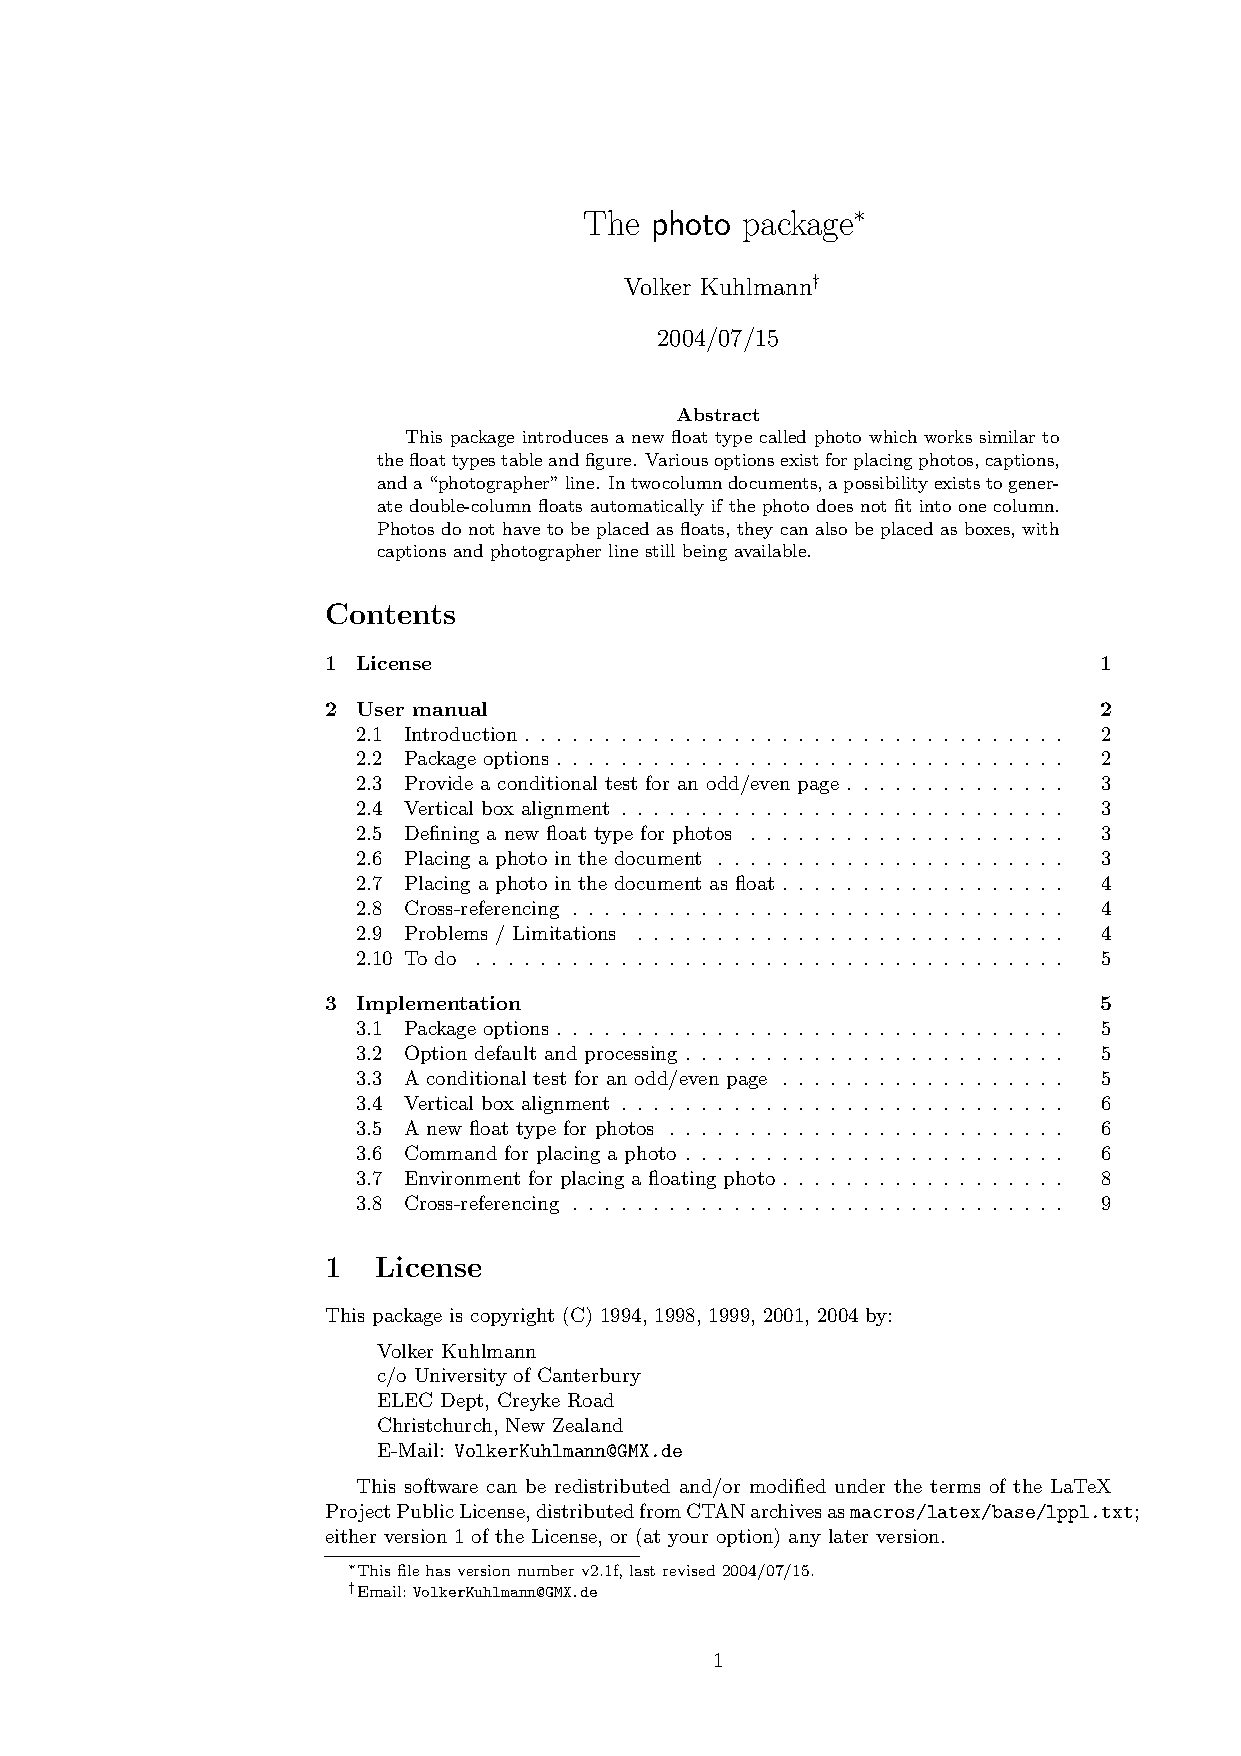
\includegraphics[bb=0 0 540 405]{photo.jpg}
\end{verbatim}
\end{quote}
It's usually not obvious what values to give the ``\texttt{bb}'' key,
but the program \ProgName{ebb} will generate a file
containing the information; the above numbers came from an
\ProgName{ebb} output file \File{photo.bb}:
\begin{quote}
\begin{verbatim}
%%Title: /home/gsm10/photo.jpg
%%Creator: ebb Version 0.5.2
%%BoundingBox: 0 0 540 405
%%CreationDate: Mon Mar  8 15:17:47 2004
\end{verbatim}
\end{quote}
However, if such a file is available, you may abbreviate the inclusion
code, above, to read:
\begin{quote}
\begin{verbatim}
\usepackage[dvipdfm]{graphicx}
...
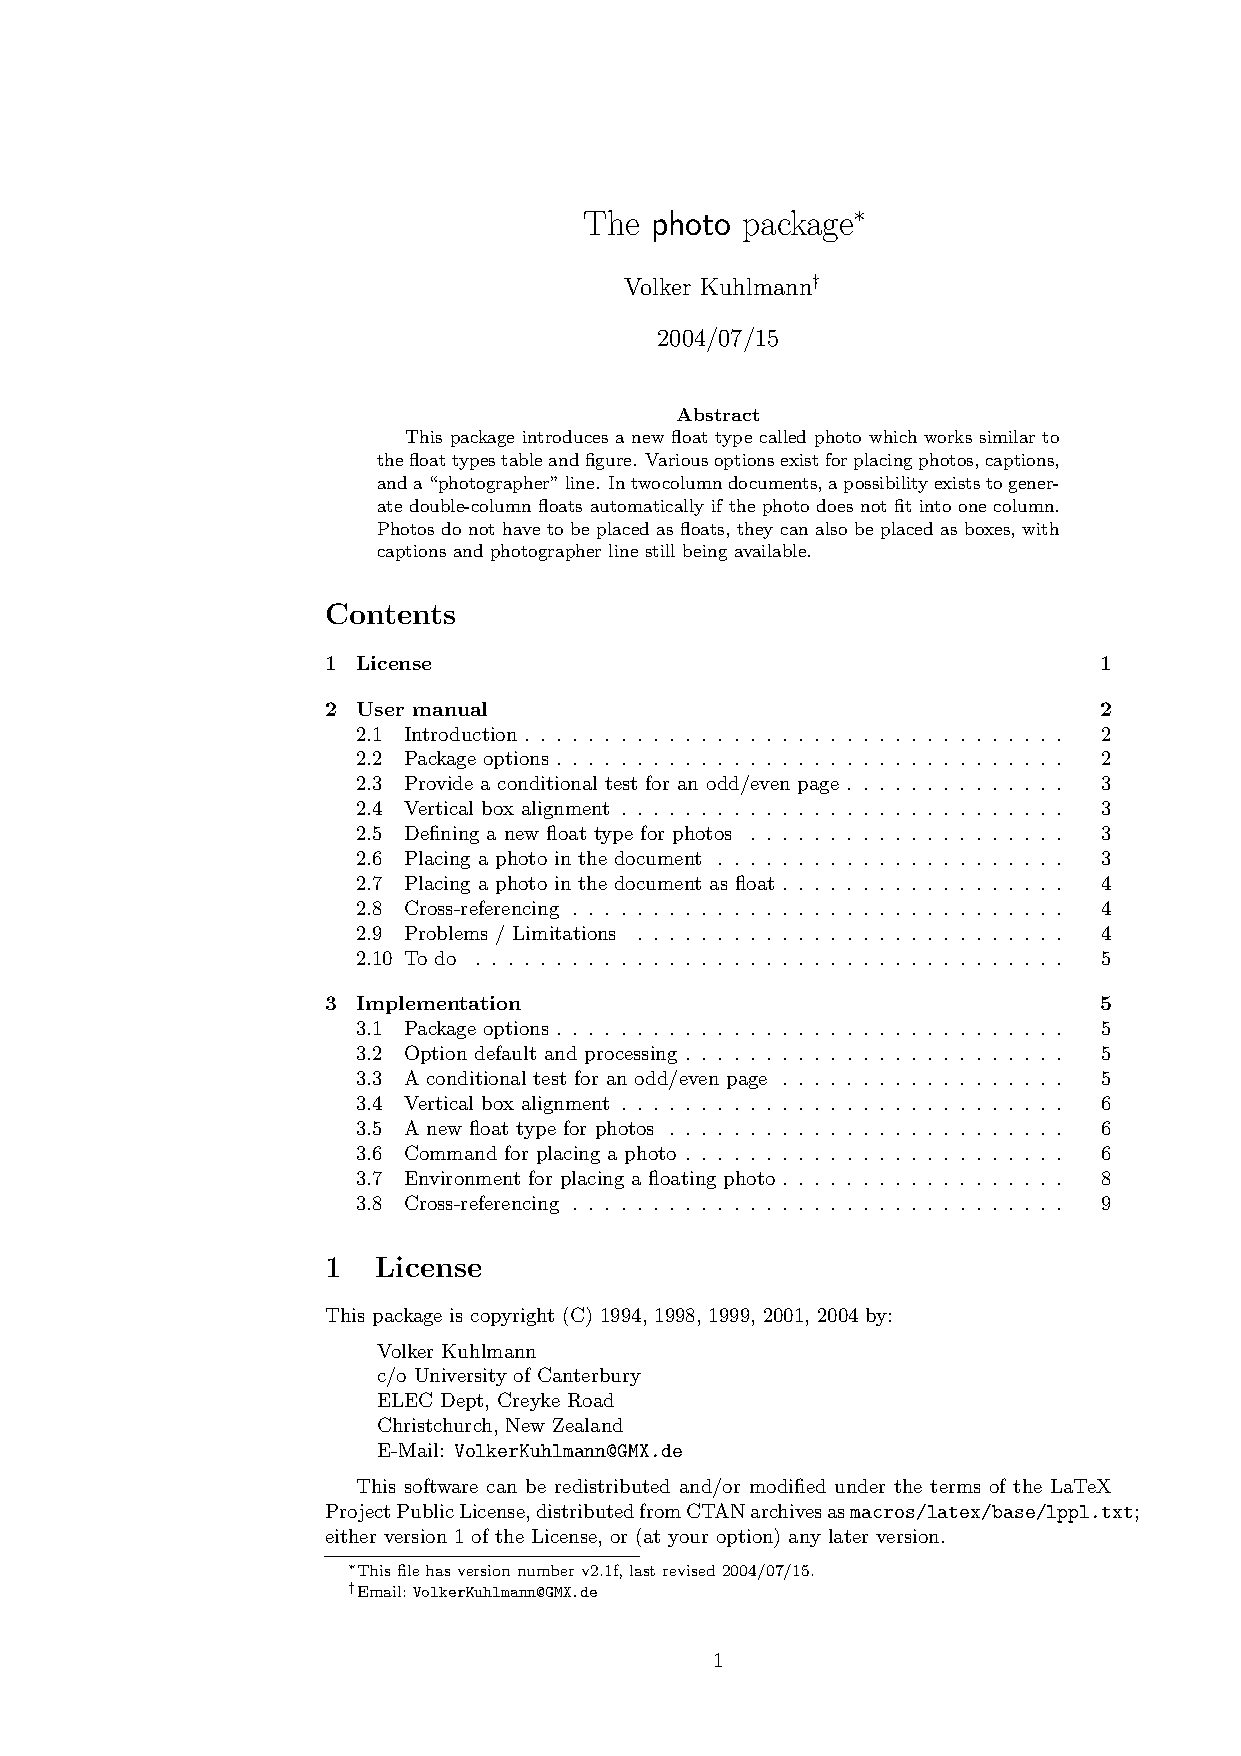
\includegraphics{photo}
\end{verbatim}
\end{quote}
which makes the operation feel as simple as does including
\texttt{.eps} images in a \LaTeX{} file for processing with
\ProgName{dvips}; the \Package{graphicx} package knows to look for a
\texttt{.bb} file if no bounding box is provided in the
\csx{includegraphics} command.

The one place where usage isn't quite so simple is the need to quote
\ProgName{dvipdfm} explicitly, as an option when loading the
\Package{graphicx} package: if you are using \ProgName{dvips}, you
don't ordinarily need to specify the fact, since the default graphics
configuration file (of most distributions) ``guesses'' the
\texttt{dvips} option if you're using \TeX{}.
\begin{ctanrefs}
\item[dvipdfm]\CTANref{dvipdfm}
\item[ebb]Distributed as part of \CTANref{dvipdfm}
\end{ctanrefs}

\Question[Q-graphicspath]{Importing graphics from ``somewhere else''}

By default, graphics commands like \csx{includegraphics} look
``wherever \TeX{} files are found'' for the graphic file they're being
asked to use.  This can reduce your flexibility if you choose to hold
your graphics files in a common directory, away from your \AllTeX{}
sources.

The simplest solution is to patch \TeX{}'s path, by changing the
default path.  On most systems, the default path is taken from the
environment variable \texttt{TEXINPUTS}, if it's present; you can adapt that
to take in the path it already has, by setting the variable to
\begin{quote}
\begin{verbatim}
TEXINPUTS=.:<graphics path(s)>:
\end{verbatim}
\end{quote}
on a Unix system; on a Windows system the separator will be ``\texttt{;}''
rather than ``\texttt{:}''.  The ``\texttt{.}'' is there to ensure
that the current directory is searched first; the trailing
``\texttt{:}'' says ``patch in the value of \texttt{TEXINPUTS} from
your configuration file, here''.

This method has the merit of efficiency (\AllTeX{} does \emph{all} of
the searches, which is quick), but it's always clumsy and may prove
inconvenient to use in Windows setups (at least).

The alternative is to use the \Package{graphics} package command
\csx{graphicspath}; this command is of course also available to users
of the \Package{graphicx} and the \Package{epsfig} packages.  The
syntax of \csx{graphicspath}'s one argument is slightly odd: it's a
sequence of paths (typically relative paths), each of which is
enclosed in braces.  A slightly odd sample, given in the
\Package{graphics} bundle documentation, is:
\begin{quote}
\begin{verbatim}
\graphicspath{{eps/}{tiff/}}
\end{verbatim}
\end{quote}
however, if the security checks on your \AllTeX{} system allow, the
path may be anything you choose (rather than strictly relative, like
those above); note that the trailing ``\texttt{/}'' \emph{is} required.

Be aware that \csx{graphicspath} does not affect the operations of
graphics macros other than those from the graphics bundle~--- in
particular, those of the outdated \Package{epsf} and
\Package{psfig} packages are immune.

The disadvantage of the \csx{graphicspath} method is inefficiency.  The
package will call \AllTeX{} once for each entry in the list, which is
itself slows things.  More seriously, \TeX{} remembers the file name,
thus effectively losing memory, every time it's
asked to look up a file, so a document that uses a huge number of
graphical inputs could be embarrassed by lack of memory.

If your document is split into a variety of directories, and each
directory has its associated graphics, the \Package{import} package
may well be the thing for you; see the discussion % beware line break
\latexhtml{of ``bits of document in other directories'' (}{in the question ``}%
\Qref{bits of document in other directories}{Q-docotherdir}%
\latexhtml{)}{''}.
\begin{ctanrefs}
\item[graphics \nothtml{\rmfamily}bundle]\CTANref{graphics}
\item[import.sty]\CTANref{import}
\end{ctanrefs}

\Question[Q-graph-pspdf]{Portable imported graphics}

A regular need is a document to be distributed in more than
one format: commonly both \PS{} and \acro{PDF}.  The
following advice is based on a post by one with much experience of
dealing with the problem of dealing with \acro{EPS} graphics in this
case.
\begin{itemize}
\item Don't specify a driver when loading loading whichever version of
  the \Package{graphics} package you use.  The scheme relies on the
  distribution's ability to decide which driver is going to be used:
  the choice is between \ProgName{dvips} and \PDFTeX{}, in this case.
  Be sure to exclude options \pkgoption{dvips}, \pkgoption{pdftex} and
  \pkgoption{dvipdfm} (\ProgName{dvipdfm} is not used in this scheme,
  but the aspirant \acro{PDF}-maker may be using it for his output,
  before switching to the scheme).
\item Use \cmdinvoke{includegraphics}[...]{filename} without
  specifying the extension (i.e., neither \texttt{.eps} nor
  \texttt{.pdf}).
\item For every \texttt{.eps} file you will be including, produce a
  \texttt{.pdf} version, as described in % beware line break
  \Qref[question]{Graphics in \PDFLaTeX{}}{Q-pdftexgraphics}.  Having
  done this, you will have two copies of each graphic (a \texttt{.eps}
  and a \texttt{.pdf} file) in your directory.
\item Use \PDFLaTeX{} (rather than
  \LaTeX{}--\ProgName{dvips}--distillation or
  \LaTeX{}--\ProgName{dvipdfm}) to produce your \acro{PDF} output.
\end{itemize}
\ProgName{Dvipdfm}'s charms are less than attractive here: the
document itself needs to be altered from its default
(\ProgName{dvips}) state, before \ProgName{dvipdfm} will process it.

\Question[Q-repeatgrf]{Repeated graphics in a document}

A logo or ``watermark'' image, or any other image that is repeated in
your document, has the potential to make the processed version of the
document unmanageably large.  The problem is, that the default
mechanisms of graphics usage add the image at every point it's to be
used, and when processed, the image appears in the output file at each
such point.

Huge \PS{} files are embarrassing; explaining \emph{why} such a file
is huge, is more embarrassing still.

The \Qref*{\File{epslatex} graphics tutorial}{Q-tutbitslatex}
describes a technique for avoiding the problem: basically, one
converts the image that's to be repeated into a \PS{} subroutine, and
load that as a \ProgName{dvips} prologue file.  In place of the image,
you load a file (with the same bounding box as the image) containing
no more than an invocation of the subroutine defined in the prologue.

The \File{epslatex} technique is tricky, but does the job.  Trickier
still is the neat scheme of converting the figure to a one-character
Adobe Type~3 outline font.  While this technique is for the ``real
experts'' only (the author of this answer has never even tried it), it has
potential for the same sort of space saving as the \File{epslatex}
technique, with greater flexibility in actual use.

More practical is Hendri Adriaens' \Package{graphicx-psmin}; you load
this \emph{in place} of \Package{graphicx}, so rather than:
\begin{quote}
\begin{verbatim}
\usepackage[<options>]{graphicx}
\end{verbatim}
\end{quote}
you will write:
\begin{quote}
\begin{verbatim}
\usepackage[<options>]{graphicx-psmin}
\end{verbatim}
\end{quote}
and at the start of your document, you write:
\begin{quote}
\begin{verbatim}
\loadgraphics[<bb>]{<list of graphics>}
\end{verbatim}
\end{quote}
and each of the graphics in the list is converted to an ``object'' for
use within the resulting \PS{} output.  (This is, in essence, an
automated version of the \File{epslatex} technique described above.)

Having loaded the package as above, whenever you use
\csx{includegraphics}, the command checks if the file you've asked for
is one of the graphics in \csx{loadgraphics}' list.  If so, the
operation is converted into a call to the ``object'' rather than a new
copy of the file; the resulting \PS{} can of course be \emph{much} smaller.

Note that the package requires a recent \ProgName{dvips}, version
5.95b (this version isn't~--- yet~--- widely distributed).

If your \PS{} is destined for conversion to \acro{PDF}, either by a
\ProgName{ghostscript}-based mechanism such as \ProgName{ps2pdf} or by
(for example) \ProgName{Acrobat} \ProgName{Distiller}, the issue isn't
so pressing, since the distillation mechanism will amalgamate graphics
objects whether or not the \PS{} has them amalgamated.  \PDFTeX{} does
the same job with graphics, automatically converting multiple uses
into references to graphics objects.
\begin{ctanrefs}
\item[graphicx-psmin.sty]\CTANref{graphicx-psmin}
\end{ctanrefs}

\Question[Q-grmaxwidth]{Limit the width of imported graphics}

Suppose you have graphics which may or may not be able to fit within
the width of the page; if they will fit, you want to set them at their
natural size, but otherwise you want to scale the whole picture so
that it fits within the page width.

You do this by delving into the innards of the graphics package (which
of course needs a little \LaTeX{} internals programming):
\begin{quote}
\begin{verbatim}
\makeatletter
\def\maxwidth{%
  \ifdim\Gin@nat@width>\linewidth
    \linewidth
  \else
    \Gin@nat@width
  \fi
}
\makeatother
\end{verbatim}
\end{quote}
This defines a ``variable'' width which has the properties you want.
Replace \csx{linewidth} if you have a different constraint on the width
of the graphic.

Use the command as follows:
\begin{quote}
\begin{verbatim}
\includegraphics[width=\maxwidth]{figure}
\end{verbatim}
\end{quote}

\Question[Q-topgraph]{Top-aligning imported graphics}

When \TeX{} sets a line of anything, it ensures that the base-line of
each object in the line is at the same level as the base-line of the
final object.  (Apart, of course, from \csx{raisebox} commands\dots{})

Most imported graphics have their base-line set at the bottom of the
picture.  When using packages such as \Package{subfig}, one often
wants to align figures by their tops.  The following odd little bit of
code does this:
\begin{quote}
\begin{verbatim}
\vtop{%
  \vskip0pt
  \hbox{%
    \includegraphics{figure}%
  }%
}
\end{verbatim}
\end{quote}
The \csx{vtop} primitive sets the base-line of the resulting object to
that of the first ``line'' in it; the \csx{vskip} creates the illusion
of an empty line, so \csx{vtop} makes the very top of the box into the
base-line.

In cases where the graphics are to be aligned with text, there is a
case for making the base-line one ex-height below the top of the box,
as in:
\begin{quote}
\begin{verbatim}
\vtop{%
  \vskip-1ex
  \hbox{%
    \includegraphics{figure}%
  }%
}
\end{verbatim}
\end{quote}
A more \LaTeX{}-y way of doing the job (somewhat innefficiently) uses
the \Package{calc} package:
\begin{quote}
\begin{verbatim}
\usepackage{calc}
...
\raisebox{1ex-\height}{\includegraphics{figure}}
\end{verbatim}
\end{quote}
(this has the same effect as the text-align version, above).

The fact is, \emph{you} may choose where the base-line ends up.  This
answer merely shows you sensible choices you might make.

\Question[Q-mpprologues]{Displaying \MP{} output in \ProgName{ghostscript}}

\MP{} ordinarily expects its output to be included in some context
where the `standard' \MF{} fonts (that you've specified) are already
defined~--- for example, as a figure in \TeX{} document.  If you're
debugging your \MP{} code, you may want to view it in
\ProgName{ghostscript} (or some other \PS{} previewer).  However,
the \PS{} `engine' in \ProgName{ghostscript} \emph{doesn't}
ordinarily have the fonts loaded, and you'll eperience an error such
as
\begin{quote}
\begin{verbatim}
Error: /undefined in cmmi10
\end{verbatim}
\end{quote}
There is provision in \MP{} for avoiding this problem: issue the
command \texttt{prologues := 2;} at the start of the \texttt{.mp} file.

Unfortunately, the \PS{} that \MP{} inserts in its output,
following this command, is incompatible with ordinary use of the
\PS{} in inclusions into \AllTeX{} documents, so it's best to
make the \texttt{prologues} command optional.  Furthermore, \MP{} takes a
very simple-minded approach to font encoding: since \TeX{} font
encodings regularly confuse sophisticated minds, this can prove
troublesome.  If you're suffering such problems (the symptom is that
characters disappear, or are wrongly presented) the only solution is
to view the `original' metapost output after processing through
\LaTeX{} and \ProgName{dvips}.

Conditional compilation may be done either
by inputting \File{MyFigure.mp} indirectly from a simple wrapper
\File{MyFigureDisplay.mp}:
\begin{quote}
\begin{verbatim}
prologues := 2;
input MyFigure
\end{verbatim}
\end{quote}
or by issuing a shell command such as
\begin{quote}
\begin{verbatim}
mp '\prologues:=2; input MyFigure'
\end{verbatim}
\end{quote}
(which will work without the quote marks if you're not using a Unix
shell).

A suitable \LaTeX{} route would involve processing
\File{MyFigure.tex}, which contains:
\begin{quote}
\begin{verbatim}
\documentclass{article}
\usepackage{graphicx}
\begin{document}
\thispagestyle{empty}
\includegraphics{MyFigure.1}
\end{document}
\end{verbatim}
\end{quote}
Processing the resulting \acro{DVI} file with the \ProgName{dvips}
command
\begin{quote}
\begin{verbatim}
dvips -E -o MyFigure.eps MyFigure
\end{verbatim}
\end{quote}
would then give a satisfactory Encapsulated \PS{} file.  This
procedure may be automated using the \ProgName{Perl} script
\ProgName{mps2eps}, thus saving a certain amount of tedium.

The Plain~\TeX{} user may use an adaptation of a jiffy of Knuth's, by
Dan Luecking.  Dan's version \Package{mpsproof.tex} will work under
\TeX{} to produce a \acro{DVI} file for use with \ProgName{dvips}, or
under \PDFTeX{} to produce a \acro{PDF} file, direct.  The output is
set up to look like a proof sheet.

A script application, \ProgName{mptopdf}, is available in recent
\AllTeX{} distributions: it seems fairly reliably to produce
\acro{PDF} from \MP{}, so may reasonably be considered an answer to
the question\dots{}
\begin{ctanrefs}
\item[mps2eps]\CTANref{mps2eps}
\item[mpsproof.tex]\CTANref{mpsproof}
\item[mptopdf]Part of \CTANref{pdftex-graphics}
\end{ctanrefs}

\Question[Q-drawing]{Drawing with \TeX{}}

There are many packages to do pictures in \AllTeX{} itself (rather than
importing graphics created externally), ranging from simple use of
\LaTeX{} \environment{picture} environment, through enhancements like
\ProgName{epic}, to 
sophisticated (but slow) drawing with \PiCTeX{}. Depending on your type
of drawing, and setup, here are a few systems you may consider:
\begin{itemize}
\item \Package{pict2e}; this was advertised in % !line break
  \Qref*{the \LaTeX{} manual}{Q-books}, but didn't appear for nearly
  ten years after publication of the book!  It removes all the petty
  niggles that surround the use of the \environment{picture}
  environment.  It therefore suffers \emph{only} from the rather
  eccentric drawing language of the environment, and is a far more
  useful tool than the original environment has ever been.  (Note that
  \Package{pict2e} supersedes David Carlisle's stop-gap
  \Package{pspicture}.)
\item \Package{pstricks}; this gives you access to all the power of
  \PS{} from \TeX{} itself, by sophisticated use of
  \Qref*{\csx{special} commands}{Q-specials}.  Since \PS{} is itself a
  pretty powerful programming language, this means there are many
  astounding things that can in principle be achieved.
  \Package{pstricks}' \csx{special}s are
  by default specific to \ProgName{dvips}, but V\TeX{} (both in its
  commercial and in its free versions) understands them.  \PDFTeX{}
  users may use \Package{pdftricks}, which (like
  \Package{epstopdf}~--- see % ! line break
  \Qref[question]{\PDFLaTeX{} graphics}{Q-pdftexgraphics}) generates
  \acro{PDF} files on the fly from \Package{pstricks} commands.  The
  documentation is good (you may browse it via the % ! line break
  \href{http://pstricks.tug.org/}{\Package{pstricks} page}
  on the \acro{TUG} web site).  There is also a mailing list
  (\mailto{pstricks@tug.org}) which you may
  \href{http://tug.org/mailman/listinfo/pstricks}{join}, or you may
  just
  browse the \href{http://tug.org/pipermail/pstricks/}{list archives}.
\item \Package{pgf}: while \Package{pstricks} is very powerful and
  convenient, using it with \PDFLaTeX{} is an awful fidget: if you
  simply want the graphical capabilities, \Package{pgf}, together with
  its rather pleasing ``user-oriented'' interface \Package{tikz}, may be a good
  bet for you.  While \acro{PDF} has (in essence) the same graphical
  capabilities as \PS{}, it isn't programmable; \Package{pgf} provides
  common \LaTeX{} commands that will utilise the graphical
  capabilities of both \PS{} and \acro{PDF} equally.
\item \MP{}; you liked \MF{}, but never got to grips with font files?
  Try \Qref*{\MP{}}{Q-MP}~---
  all the power of \MF{}, but it generates \PS{} figures; \MP{}
  is nowadays part of most serious \AllTeX{} distributions.  Knuth
  uses it for all his work\dots{}
\item \ProgName{Mfpic}; you liked \MF{}, but can't understand the
  language?  The package makes up \MF{} or \MP{} code for you
  within using familiar-looking \TeX{} macros.  Not \emph{quite} the
  full power of \MP{}, but a friendlier interface; of course, with
  \MP{} output, the results can be used equally well in either
  \LaTeX{} or \PDFLaTeX{}.
\item You liked \PiCTeX{} but don't have enough memory or time?  Look
  at Eitan Gurari's \Package{dratex}, which is as powerful as most
  other \TeX{} drawing packages, but is an entirely new
  implementation, which is not as hard on memory, is much more
  readable (and is fully documented).
\end{itemize}
\begin{ctanrefs}
\item[dratex.sty]\CTANref{dratex}
\item[mfpic]\CTANref{mfpic}
\item[pdftricks.sty]\CTANref{pdftricks}
\item[pspicture.sty]\CTANref{pspicture}
\item[pgf.sty]\CTANref{pgf}
\item[pict2e.sty]\CTANref{pict2e}
\item[pstricks]\CTANref{pstricks}
\item[tikz.sty]Distributed with \CTANref{pgf}
\end{ctanrefs}

\Question[Q-drawFeyn]{Drawing Feynman diagrams in \LaTeX{}}

Michael Levine's \Package{feynman} bundle for drawing the diagrams in
\LaTeXo{} is still available.

Thorsten Ohl's \Package{feynmf} is designed for use with current
\LaTeX{}, and works in
combination with \MF{} (or, in its \Package{feynmp} incarnation, with
\MP{}).  The \ProgName{feynmf} or
\ProgName{feynmp} package reads a description of the diagram written
in \TeX{}, and writes out code.  \MF{} (or \MP{}) can then produce a
font (or \PS{} file) for use in a subsequent \LaTeX{} run.  For
new users, who have access to \MP{}, the \PS{} version is
probably the better route, for document portability and other reasons.
% checked rf 2001/03/22

Jos Vermaseren's \Package{axodraw} is mentioned as an alternative in
the documentation of \Package{feynmf}, but it is written entirely in
terms of \ProgName{dvips} \csx{special} commands, and is thus rather
imperfectly portable.

An alternative approach is implemented by Norman Gray's \Package{feyn}
package.  Rather than creating complete diagrams as postscript images,
\Package{feyn} provides a font (in a variety of sizes) containing
fragments, which you can compose to produce complete diagrams.  It
offers fairly simple diagrams which look good in equations, rather
than complicated ones more suitable for display in figures.
\begin{ctanrefs}
\item[axodraw]\CTANref{axodraw}
\item[feyn \nothtml{\rmfamily}font bundle]\CTANref{feyn}
\item[feynman bundle]\CTANref{feynman}
\item[feynmf/feynmp bundle]\CTANref{feynmf}
\end{ctanrefs}

\Question[Q-labelfig]{Labelling graphics}

``Technical'' graphics (such as graphs and diagrams) are often
labelled with quite complex mathematical expressions: there are few
drawing or graphing tools that can do such things (the honourable
exception being \MP{}, which allows you to program the labels, in
\AllTeX{}, in the middle of specifying your graphic).

Labels on graphics produced by all those \emph{other} tools is where
the \Package{psfrag} package can help.  Place an unique
text in your graphic, using the normal text features of your tool, and
you can ask \Package{psfrag} to replace the text with arbitrary
\AllTeX{} material.  \Package{Psfrag}'s ``operative'' command is
\cmdinvoke{psfrag}{\emph{PS text}}{\emph{Repl text}}, which instructs
the system to replace the original (``\texttt{PS}'') text with the
\TeX{}-typeset replacement text.  Optional
arguments permit adjustment of position, scale and rotation; full
details may be found in \File{pfgguide} in the distribution.
(Unfortunately, \Package{psfrag} can't be used with \PDFLaTeX{},
though one might hope that it would be susceptible to the same sort of
treatment as is used in the \Package{pdftricks} package.  On the other
hand,
\begin{narrowversion}
  V\TeX{}'s GeX processor (\Qref{}{Q-commercial})
\end{narrowversion}
\begin{wideversion}
  \Qref*{V\TeX{}}{Q-commercial}'s GeX processor
\end{wideversion}
explicitly deals with \Package{psfrag}, both in its free and
commercial instances.)

The \Package{psfragx} package goes one step further than
\Package{psfrag}: it provides a means whereby you can put the
\Package{psfrag} commands into the preamble of your \acro{EPS} file
itself.  \Package{Psfrag} has such a command itself, but deprecates
it; \Package{psfragx} has cleaned up the facility, and provides a
script \ProgName{laprint} for use with \ProgName{Matlab} to produce
appropriately tagged output.  (In principle, other graphics
applications could provide a similar facility, but apparently none does.)

\ProgName{Emacs} users may find the embedded editor \ProgName{iTe} a
useful tool for placing labels: it's a \AllTeX{}-oriented graphical
editor written in \ProgName{Emacs Lisp}.  You create
\environment{iteblock} environments containing graphics and text, and
may then invoke \ProgName{iTe} to arrange the elements relative to one
another.

Another useful approach is \Package{overpic}, which overlays a
\environment{picture} environment on a graphic included by use of
\csx{includegraphics}.  This treatment lends itself to ready placement
of texts and the like on top of a graphic.  The package can draw a
grid for planning your ``attack''; the distribution comes with simple
examples.

\Package{Pstricks} can of course do everything that \Package{overpic}
can, with all the flexibility of \PS{} programming that it offers
The \Package{pstricks} web site has a page with several % ! line break
\href{http://pstricks.tug.org/main.cgi?file=Examples/overlay}{examples of labelling}
which will get you started; if \Package{pstricks} is % ! line break
\Qref*{an option for you}{Q-drawing}, this route is worth a try.

The confident user may, of course, do the whole job in a picture
environment which itself includes the graphic.  I would recommend
\Package{overpic} or the \Package{pstricks} approach, but such things
are plainly little more than a convenience over what is achievable
with the do-it-yourself approach.
\begin{ctanrefs}
\item[iTe]\CTANref{ite}
\item[laprint]Distributed with \CTANref{psfragx}
\item[overpic.sty]\CTANref{overpic}
\item[psfrag.sty]\CTANref{psfrag}
\item[psfragx.sty]\CTANref{psfragx}
\item[pstricks.sty]\CTANref{pstricks}
\end{ctanrefs}

%%%%%%%%%%%%%%%%%%%%%%%%%%%%%%%%%%%%%%%%%%%%%%%%%%%%%%%%%%%%%%%%%

\section{Bibliographies and citations}

\subsection{Creating bibliographies}

\Question[Q-buildbib]{Creating a \BibTeX{} bibliography file}

A \BibTeX{} bibliography file may reasonably be compared to a small
database, the entries in which are references to literature that may
be called up by citations in a document.

Each entry in the bibliography has a \emph{type} and a unique
\emph{key}.  The bibliography is read, by \BibTeX{}, using the details
specified in a \emph{bibliography style}.  From the style, \BibTeX{}
finds what entry types are permissible, what \emph{fields} each entry
type has, and how to format the whole entry.

The type specifies the type of document you're making reference to; it
may run all the way from things like ``\environment{Book}'' and
``\environment{Proceedings}'' (which may even contain other citations
of type ``\environment{InBook}'' or  ``\environment{InProceedings}'')
through dissertation styles like  ``\environment{PhdThesis}'' to
otherwise-uncategorisable things such as ``\environment{Misc}''.  The
unique key is something you choose yourself: it's what you use when
you want to \Qref*{cite an entry in the file}{Q-usebibtex}.  People
commonly create a key that combines the (primary) author's name and
the year of publication, possibly with a marker to distinguish
publications in the same year.  So, for example, the Dyson, Eddington,
Davidson paper about deflection of starlight appears in my
experimental \texttt{.bib} file as \texttt{Dyson20.1}.

So, noting the rules of the style, you have `simply' to write a
bibliography database.  Fortunately, there are several tools to help
in this endeavour:
\begin{itemize}
\item Most of the better \Qref*{\AllTeX{}-oriented editors}{Q-editors}
  have ``\BibTeX{} modes''.
\item If you have an existing \environment{thebibliography}
  environment, the \ProgName{Perl} script \ProgName{tex2bib} will
  probably help.
\item There are a number of \BibTeX{} bibliography management systems
  available, some of which permit a graphical user interface to the
  task.  Sadly, none seems to be available with the ordinary \TeX{}
  distributions.
  
  Tools such as \ProgName{Xbibfile} (a graphical user interface),
  \ProgName{ebib} (a database application written to run `inside'
  \ProgName{emacs}) and 
  \ProgName{btOOL} (a set of \ProgName{perl} tools for building 
  \BibTeX{} database handlers) are available from \acro{CTAN}.

  Other systems, such as
  \href{http://refdb.sourceforge.net/}{\ProgName{RefDB}},
  \href{http://www.nongnu.org/biborb}{BibORB},
  \href{http://bibdesk.sourceforge.net/}{\ProgName{BibDesk}},
  \href{http://pybliographer.org}{\ProgName{pybliographer}} and the
  \ProgName{Java}-based
  \href{http://freshmeat.net/projects/bibkeeper/}{\ProgName{Bibkeeper}}
  and \href{http://jabref.sourceforge.net}{\ProgName{JabRef}} (which
  claims to supersede \ProgName{Bibkeeper})
  are only available from their development sites.
% review of web database offerings in textex_368
\item Some commercial citation-management systems will export in
  \BibTeX{} format; an example is
  \href{http://www.endnote.com/}{EndNote}.
\item Data from on-line citation databases may often be translated to
  \BibTeX{} format by utilities to be found on \acro{CTAN}.  For
  example, the \ProgName{Perl} script \ProgName{isi2bibtex} will
  translate citations from \acro{ISI} ``Web of knowledge'' (a
  subscription service, available to \acro{UK} academics via
  \acro{BIDS}).  UK academics may translate \acro{BIDS} downloads
  using \ProgName{bids.to.bibtex}
\end{itemize}
\begin{ctanrefs}
\item[bids.to.bibtex]\CTANref{bidstobibtex}
\item[btOOL]\CTANref{btOOL}
\item[ebib]\CTANref{ebib}
\item[isi2bibtex]\CTANref{isi2bibtex}
\item[tex2bib]\CTANref{tex2bib}
\item[tex2bib.readme]\CTANref{tex2bib-doc}
\item[xbibfile]\CTANref{xbibfile}
\end{ctanrefs}

\Question[Q-custbib]{Creating a bibliography style}

It \emph{is} possible to write your own: the standard bibliography
styles are distributed in a commented form, and there is a description
of the language (see
% beware line-wrap
\Qref[question]{BibTeX documentation}{Q-BibTeXing}).
However, it must be admitted that the language in which \BibTeX{}
styles are written is pretty obscure, and one would not recommend
anyone who's not a confident programmer to write their own, though
minor changes to an existing style may be within the grasp of many.

If your style isn't too `far out', you can probably generate it by
using the facilities of the \Package{custom-bib} bundle.  This
contains a file \File{makebst.tex}, which runs you through a text menu
to produce a file of instructions, with which you can generate your
own \texttt{.bst} file.  This technique doesn't offer entirely new styles
of document, but the system's ``master \BibTeX{} styles'' already
offer significantly more than the \BibTeX{} standard set.
\begin{ctanrefs}
\item[\nothtml{\normalfont}\BibTeX{} documentation]\CTANref{bibtex-doc}
\item[makebst.tex]Distributed with \CTANref{custom-bib}
\end{ctanrefs}

\Question[Q-capbibtex]{Capitalisation in \BibTeX{}}

The standard \BibTeX{} bibliography styles impose fixed ideas about
the capitalisation of titles of things in the bibliography.  While
this is not unreasonable by \BibTeX{}'s lights (the rules come from
the \emph{Chicago Manual of Style}) it can be troublesome, since
\BibTeX{} fails to recognise special uses (such as acronyms, chemical
formulae, etc.).

The solution is to enclose the letter or letters, whose capitalisation
\BibTeX{} should not touch, in braces, as:
\begin{quote}
\begin{verbatim}
title = {The {THE} operating system},
\end{verbatim}
\end{quote}
Sometimes you find \BibTeX{} changing the case of a single letter
inappropriately.  No matter: the technique can be applied to single
letters, as in:
\begin{quote}
\begin{verbatim}
title = {Te{X}niques and tips},
\end{verbatim}
\end{quote}
If your document design specification requires a different style of
capitalisation, you should acquire a bibliography style that doesn't
enforce \BibTeX{}'s default rules.  It is definitely \emph{not} a good
idea to enclose an entire title in braces, as in
\begin{quote}
\begin{verbatim}
title = {{TeXniques and tips}},
\end{verbatim}
\end{quote}
though that does ensure that the capitalisation is not changed.  Your
\BibTeX{} database should be a general-purpose thing, not something
tuned to the requirements of a particular document, or to the way you
are thinking today.

There's more on the subject in the
% beware line wrap
\Qref*{\BibTeX{} documentation}{Q-BibTeXing}.

\Question[Q-bibaccent]{Accents in bibliographies}

\BibTeX{} not only has a tendency (by default) to mess about with the
% line wrap
\Qref*{case of letters in your bibliography}{Q-capbibtex},
also makes a hash of accent commands:
\begin{htmlversion}
``\texttt{ma\~nana}'' comes out as ``ma nana'' (!).  The solution is
similar: enclose the troublesome sequence in braces, as
``|{|\texttt{\~n}|}|'', in this example.
\end{htmlversion}
\htmlignore
``|ma\~nana|'' comes out as ``ma nana'' (!).  The solution is similar:
enclose the troublesome sequence in braces, as ``|{\~n}|'', in this
example.
\endhtmlignore

\Question[Q-bibstrtl]{`String too long' in \BibTeX{}}

The \BibTeX{} diagnostic ``Warning--you've exceeded 1000, the
\texttt{global-string-size}, for entry \texttt{foo}'' usually arises
from a very large abstract or annotation included in the database.
The diagnostic usually arises because of an infelicity in the coding of
\File{abstract.bst}, or styles derived from it.  (One doesn't
ordinarily output annotations in other styles.)

The solution is to make a copy of the style file (or get a clean copy
from \acro{CTAN}~--- \CTANref{abstract-bst}), and rename it (e.g., on a
long file-name system, to \File{abstract-long.bst}).  Now edit it: find
function \texttt{output.nonnull} and
\begin{itemize}
\item change its first line (line 60 in the version on \acro{CTAN})
  from
  \begin{quote}
\begin{verbatim}
{ 's :=
\end{verbatim}
  \end{quote}
to
  \begin{quote}
\begin{verbatim}
{ swap$
\end{verbatim}
  \end{quote}
  Finally,
\item delete the function's last line, which just says ``\texttt{s}
  (line 84 in the version on \acro{CTAN}).
\end{itemize}
Finally, change your \csx{bibliographystyle} command to refer to the
name of the new file.

This technique applies equally to any bibliography style: the same
change can be made to any similar \texttt{output.nonnull} function.

If you're reluctant to make this sort of change, the only way forward
is to take the entry out of the database, so that you don't encounter
\BibTeX{}'s limit, but you may need to retain the entry because it
will be included in the typeset document.  In such cases, put the body
of the entry in a separate file:
\begin{quote}
\begin{verbatim}
@article{long.boring,
  author =    "Fred Verbose",
  ...
  abstract =  "{\input{abstracts/long.tex}}"
}
\end{verbatim}
\end{quote}
In this way, you arrange that all \BibTeX{} has to deal with is the
file name, though it will tell \TeX{} (when appropriate) to include
all the long text.

\Question[Q-manyauthor]{\BibTeX{} doesn't understand lists of names}

\BibTeX{} has a strict syntax for lists of authors' (or editors')
names in the \BibTeX{} data file; if you write the list of names in a
``natural''-seeming way, the chances are you will confuse \BibTeX{},
and the output produced will be quite different from what you had
hoped.

Names should be expressed in one of the forms
\begin{quote}
\begin{verbatim}
First Last
Last, First
Last, Suffix, First
\end{verbatim}
\end{quote}
and lists of names should be separated with ``\texttt{and}''.
For example:
\begin{quote}
\begin{verbatim}
AUTHOR = {Fred Q. Bloggs, John P. Doe \&
          Another Idiot}
\end{verbatim}
\end{quote}
falls foul of two of the above rules: a syntactically significant
comma appears in an incorrect place, and `\csx{\&}' is being used as a
name separator.  The output of the above might be something like:
\begin{quote}
\begin{wideversion}
\begin{verbatim}
John P. Doe \& Another Idiot Fred Q. Bloggs
\end{verbatim}
\end{wideversion}
\begin{narrowversion}
\begin{verbatim}
John P. Doe \& Another Idiot
                        Fred Q. Bloggs
\end{verbatim}
\end{narrowversion}
\end{quote}
because ``John P. Doe \& Another Idiot has become the `first name',
while ``Fred Q. Bloggs'' has become the `last name' of a single
person.  The example should have been written:
\begin{quote}
\begin{narrowversion}
\begin{verbatim}
AUTHOR = {Fred Q. Bloggs and
          John P. Doe and
          Another Idiot}
\end{verbatim}
\end{narrowversion}
\begin{wideversion}
\begin{verbatim}
AUTHOR = {Fred Q. Bloggs and John P. Doe and
          Another Idiot}
\end{verbatim}
\end{wideversion}
\end{quote}
Some bibliography styles implement clever acrobatics with very long
author lists.  You can force truncation by using the pseudo-name
``|others|'', which will usually translate to something like
``\emph{et al}'' in the typeset output.  So, if Mr.~Bloggs wanted to
distract attention from his co-authors, he would write:
\begin{quote}
\begin{verbatim}
AUTHOR = {Fred Q. Bloggs and others}
\end{verbatim}
\end{quote}

\Question[Q-citeURL]{\acro{URL}s in \BibTeX{} bibliographies}

There is no citation type for \acro{URL}s, \emph{per se}, in the
standard \BibTeX{} styles, though Oren Patashnik (the author of
\BibTeX{}) is believed to beconsidering developing one such for use
with the long-awaited \BibTeX{} version~1.0.

The actual information that need be available in a citation of an
\acro{URL} is discussed at some length in the publicly available
on-line 
\begin{narrowversion}
  extracts of \acro{ISO}~690--2, available via
  \URL{http://www.nlc-bnc.ca/iso/tc46sc9/standard/690-2e.htm};
  % checked 2004-01-15
\end{narrowversion}
\begin{wideversion}
\href{http://www.nlc-bnc.ca/iso/tc46sc9/standard/690-2e.htm}{extracts of \acro{ISO}\nobreakspace690--2};
\end{wideversion}
the techniques below do \emph{not} satisfy all the requirements of
\acro{ISO}~690--2, but they offer a solution that is at least
available to users of today's tools.

Until the new version of \BibTeX{} arrives, the simplest technique is
to use the \texttt{howpublished} field of the standard styles' \texttt{@misc}
function.  Of course, the strictures
about \Qref*{typesetting \acro{URL}s}{Q-setURL} still apply, so the
entry will look like:
\begin{quote}
\begin{verbatim}
@misc{...,
  ...,
  howpublished = "\url{http://...}"
}
\end{verbatim}
\end{quote}
A possible alternative approach is to use \BibTeX{} styles other than
the standard ones, that already have \acro{URL} entry types.
Candidates are:
\begin{itemize}
\item The \Package{natbib} styles (\Package{plainnat},
  \Package{unsrtnat} and \Package{abbrevnat}), which are extensions of
  the standard styles, principally for use with \Package{natbib}
  itself.  However, they've acquired \acro{URL}s and other ``modern''
  entries along the way.  The same author's \Package{custom-bib} is
  also capable of generating styles that honour \acro{URL} entries.
\item The \Package{babelbib} bundle, which offers % ! line break
  \Qref*{multilingual bibliographies}{Q-i18nbib}, similarly provides a
  set of standard-style equivalents that have \acro{URL} entries.
\item More modern styles such as the \Package{harvard} package (if the
  citation styles are otherwise satisfactory for you).
  \Package{Harvard} bibliography styles all include a ``\texttt{url}''
  field in their specification; however, the typesetting offered is
  somewhat feeble (though it does recognise and use
  \ProgName{LaTeX2HTML} macros if they are available, to create
  hyperlinks).
\end{itemize}
You can also acquire new \BibTeX{} styles by use of Norman Gray's
\Package{urlbst} system, which is based on a \ProgName{Perl} script
that edits an existing \BibTeX{} style file to produce a new
style. The new style thus generated has a |webpage| entry type, and
also offers support for |url| and |lastchecked| fields in the other entry
types.  The \ProgName{Perl} script comes with a set of converted
versions of the standard bibliography styles.  Documentation is
distributed as \LaTeX{} source.

Another possibility is that some conventionally-published paper,
technical report (or even book) is also available on the Web.  In such
cases, a useful technique is something like:
\begin{quote}
\begin{wideversion}
\begin{verbatim}
@techreport{...,
  ...,
  note = "Also available as \url{http://...}"
}
\end{verbatim}
\end{wideversion}
\begin{narrowversion}
\begin{verbatim}
@techreport{...,
  ...,
  note = "Also available as 
                       \url{http://...}"
}
\end{verbatim}
\end{narrowversion}
\end{quote}
There is good reason to use the \Package{url} or \Package{hyperref}
packages in this context: \BibTeX{} has a habit of splitting
lines it considers excessively long, and if there are no space
characters for it to use as `natural' breakpoints, \BibTeX{} will
insert a comment (`\texttt{\textpercent}') character~\dots{}\@ which
is an acceptable character in an \acro{URL}.  Any current version of the
\Package{url} or \Package{hyperref} package detects this
``\texttt{\textpercent}--end-of-line'' structure in its argument, and
removes it.
\begin{ctanrefs}
\item[babelbib \nothtml{\rmfamily}bundle]\CTANref{babelbib}
\item[custom-bib \nothtml{\rmfamily}bundle]\CTANref{custom-bib}
\item[harvard.sty]\CTANref{harvard}
\item[hyperref.sty]\CTANref{hyperref}
\item[natbib \nothtml{\rmfamily}styles]\CTANref{natbib}
\item[url.sty]\CTANref{url}
\item[urlbst]\CTANref{urlbst}
\end{ctanrefs}

\Question[Q-bibplain]{Using \BibTeX{} with Plain \TeX{}}

The file \File{btxmac.tex} (which is part of the \Eplain{} system)
contains macros and documentation for using \BibTeX{} with Plain
\TeX{}, either directly or with \Qref*{\Eplain{}}{Q-eplain}.  See
\Qref[question]{the use of \BibTeX{}}{Q-BibTeXing} for more
information about \BibTeX{} itself.
\begin{ctanrefs}
\item[btxmac.tex]\CTANref{btxmactex}
\item[eplain \nothtml{\rmfamily}system]\CTANref{eplain}
\end{ctanrefs}

\Question[Q-makebib]{Reconstructing \texttt{.bib} files}

Perhaps you've lost the \texttt{.bib} file you generated your document from,
or have been sent a document without one.  Or even, you've realised
the error of building a substantial document without the benefit of
\BibTeX{}\dots{}

The \ProgName{Perl} script, \Package{tex2bib} makes a reasonable job
of regenerating |.bib| files from \environment{thebibliography}
environments, provided that the original (whether automatically or
manually generated) doesn't deviate too far from the ``standard''
styles.

You are well-advised to check the output of the script.  While it will
not usually destroy information, it can quite reasonably mislabel it.

Documentation of the script is to be found in the file \File{tex2bib.readme}
\begin{ctanrefs}
\item[tex2bib]\CTANref{tex2bib}
\item[tex2bib.readme]\CTANref{tex2bib-doc}
\end{ctanrefs}

\Question[Q-bibprefixsort]{\BibTeX{} sorting and name prefixes}

\BibTeX{} recognises a bewildering array of name prefixes (mostly
those deriving from European language names); it ignores the prefixes
when sorting the bibliography~--- you want ``Ludwig van Beethoven''
sorted under ``Beethoven'', not under ``van''.  (Lamport made a witty
deliberate mistake with Beethoven's name, in the first edition of his
\LaTeX{} manual.)

However, a recurring issue is the desire to quote Lord Rayleigh's
publications (``Lord'' isn't an acceptable prefix), or names from
languages that weren't considered when \BibTeX{} was designed such as
``al-Wakil'' (transcribed from the Arabic).  What's needed is a
separate ``sort key'', but \BibTeX{} only allows such a thing in
citations of items that have no author or editor.

The solution is to embed the sort key in the author's name, but to
prevent it from being typeset.  Patashnik recommends a command
\csx{noopsort} (no-output-sortkey), which is defined and used as
follows:
\begin{quote}
\begin{wideversion}
\begin{verbatim}
@PREAMBLE{ {\providecommand{\noopsort}[1]{}} }
...
@ARTICLE{Rayleigh1,
AUTHOR = "{\noopsort{Rayleigh}}{Lord Rayleigh}",
...
}
\end{verbatim}
\end{wideversion}
\begin{narrowversion}
\begin{verbatim}
@PREAMBLE{
    {\providecommand{\noopsort}[1]{}}
}
...
@ARTICLE{Rayleigh1,
AUTHOR = 
   "\noopsort{Rayleigh}{Lord Rayleigh}",
...
}
\end{verbatim}
\end{narrowversion}
\end{quote}
Note that this \csx{noopsort} applies to the last name in this kind of
construct, so an author with an Arabic name might be rendered:
\begin{wideversion}
\begin{quote}
\begin{verbatim}
...
AUTHOR = "Ali {\noopsort{Hadiidii}}{al-Hadiidii}",
...
\end{verbatim}
\end{quote}
\end{wideversion}
\begin{narrowversion}
\begin{quote}
\begin{verbatim}
...
AUTHOR = 
   "Ali {\noopsort{Hadiidii}}{al-Hadiidii}",
...
\end{verbatim}
\end{quote}
\end{narrowversion}
A further use might deal with word order games, as in the famous
Vietnamese name:
\begin{wideversion}
\begin{quote}
\begin{verbatim}
...
AUTHOR = "\noopsort{Thanh Han The}{Han The Thanh}",
...
\end{verbatim}
\end{quote}
\end{wideversion}
\begin{narrowversion}
\begin{quote}
\begin{verbatim}
...
AUTHOR =
   "\noopsort{Thanh Han The}{Han The Thanh}",
...
\end{verbatim}
\end{quote}
\end{narrowversion}
though that author seems well-acquainted with Western confusion about
the significance of the parts of his name (even to the extent of
missing out the accentuation, as above\dots{}).

\Question[Q-bibtranscinit]{Transcribed initials in \BibTeX{}}

If your bibliographic style uses initials~+ surname, you may encounter
a problem with some transcribed names (for example, Russian ones).
Consider the following example from the real world:
\begin{quote}
\begin{narrowversion}
\begin{verbatim}
@article{epifanov1997,
   author = {Epifanov, S. Yu. and
             Vigasin, A. A.},
   title  = ...
}
\end{verbatim}
\end{narrowversion}
\begin{wideversion}
\begin{verbatim}
@article{epifanov1997,
   author = {Epifanov, S. Yu. and Vigasin, A. A.},
   title  = ...
}
\end{verbatim}
\end{wideversion}
\end{quote}
Note that the ``Yu'' is the initial, not a complete name. However,
\BibTeX{}'s algorithms will leave you with a citation~--- 
slightly depending on the bibliographic style~--- that reads:
``S. Y. Epifanov and A. A. Vigasin, \dots{}''. instead of the intended
``S. Yu. Epifanov and A. A. Vigasin, \dots{}''.

One solution is to replace each affected initial by a command that 
prints the correct combination.  To keep your bibliography portable,
you need to add that command to your bibliography with the
\texttt{@preamble} directive:
\begin{quote}
\begin{narrowversion}
\begin{verbatim}
@preamble{ {\providecommand{\BIBYu}{Yu} } }

@article{epifanov1997,
   author   = {Epifanov, S. {\BIBYu}. and
               Vigasin, A. A.},
   title    = ...
}
\end{verbatim}
\end{narrowversion}
\begin{wideversion}
\begin{verbatim}
@preamble{ {\providecommand{\BIBYu}{Yu} } }

@article{epifanov1997,
   author   = {Epifanov, S. {\BIBYu}. and Vigasin, A. A.},
   title    = ...
}
\end{verbatim}
\end{wideversion}
\end{quote}
If you have many such commands, you may want to put them in a separate
file and \csx{input} that \LaTeX{} file in a \texttt{@preamble}
directive.

An alternative is to make the transcription look like an accent, from
\BibTeX{}'s point of view.  For this we need a control sequence that
does nothing:
\begin{quote}
\begin{verbatim}
@article{epifanov1997,
   author   = {Epifanov, S. {\relax Yu}. and Vigasin, A. A.},
   title    = ...
}
\end{verbatim}
\end{quote}
Like the solution by generating extra commands, this involves tedious
extra typing; which of the two techniques is preferable for a given
bibliography will be determined by the names in it.

\subsection{Creating citations}

\Question[Q-usebibtex]{``Normal'' use of \BibTeX{} from \LaTeX{}}

To create a bibliography for your document, you need to perform a
sequence of steps, some of which seem a bit odd.  If you choose to use
\BibTeX{}, the sequence is:

First: you need a \BibTeX{} bibliography file (a |.bib| file)~--- see
\nothtml{``creating a \BibTeX{} file'' (\Qref[question]{}{Q-buildbib}).}
\begin{htmlversion}
``\Qref[question]{creating a \BibTeX{} file}{Q-buildbib}''.
\end{htmlversion}

Second: you must write your \LaTeX{} document to include a declaration
of the `style' of bibliography, citations, and a reference to the
bibliography file mentioned in the step 1.  So we may have a \LaTeX{}
file containing:
\begin{quote}
\begin{verbatim}
\bibliographystyle{plain}
...
Pooh is heroic~\cite{Milne:1926}.
...
Alice struggles~\cite{Carroll:1865}.
...
\bibliography{mybooks}
\end{verbatim}
\end{quote}
Note: we have bibliography style \Package{plain}, above, which is
nearly the simplest of the lot: a sample text, showing the sorts of
style choices available, can be found on Ken Turner's web site:
\URL{http://www.cs.stir.ac.uk/~kjt/software/latex/showbst.html}

Third: you must process the file.
\begin{quote}
\begin{verbatim}
latex myfile
\end{verbatim}
\end{quote}
As \LaTeX{} processes the file, the \csx{bibliographystyle} command
writes a note of the style to the |.aux| file; each \csx{cite} command
writes a note of the citation to the |.aux| file, and the
\csx{bibliography} command writes a note of which |.bib| file is to be
used, to the |.aux| file.

Note that, at this stage, \LaTeX{} isn't ``resolving'' any of the
citations: at every \csx{cite} command, \LaTeX{} will warn you of the
undefined citation, and when the document finishes, there will be a
further warning of undefined references.

%Some bibliography styles are designed to work with particular
%packages...

Fourth: you must run \BibTeX{}:
\begin{quote}
\begin{verbatim}
bibtex myfile
\end{verbatim}
\end{quote}
Don't try to tell \BibTeX{} anything but the file name: say
\texttt{bibtex myfile.aux} (because you know it's going to read the
|.aux| file) and \BibTeX{} will blindly attempt to process
\texttt{myfile.aux.aux}.

\BibTeX{} will scan the |.aux| file; it will find which bibliography
style it needs to use, and will ``compile'' that style; it will note
the citations; it will find which bibliography files it needs, and
will run through them matching citations to entries in the
bibliography; and finally it will sort the entries that have been
cited (if the bibliography style specifies that they should be
sorted), and outputs the resulting details to a |.bbl| file.

Fifth: you run \LaTeX{} again.  It warns, again, that each citation is
(still) undefined, but when it gets to the \csx{bibliography} command,
it finds a |.bbl| file, and reads it.  As it encounters each
\csx{bibitem} command in the file, it notes a definition of the
citation.

Sixth: you run \LaTeX{} yet again.  This time, it finds values for all
the citations, in its |.aux| file.  Other things being equal, you're
done\dots{} until you change the file.

If, while editing, you change any of the citations, or add new ones,
you need to go through the process above from steps 3 (first run of
\LaTeX{}) to 6, again, before the document is once again stable.
These four mandatory runs of \LaTeX{} make processing a document with
a bibliography even more tiresome than the normal two runs required to
resolve labels.

To summarise: processing to resolve citations requires: \LaTeX{};
\BibTeX{}; \LaTeX{}; \LaTeX{}.

\Question[Q-whatbst]{Choosing a bibliography style}

A large proportion of people are satisfied with one of Patashnik's
original ``standard'' styles, \Package{plain}, \Package{unsrt},
\Package{abbrv} and \Package{alpha}.  However, no style in that set
supports the ``author-date'' citation style that is popular in many
fields; but there are a very large number of contributed styles
available, that \emph{do} support the format.

(Note that author-date styles arose because the simple and clear
citation style that \Package{plain} produces is so awkward in a
traditional manuscript preparation scenario.  However, \TeX{}-based
document production does away with all those difficulties, leaving us
free once again to use the simple option.)

Fortunately, help is at hand, on the Web, with this problem:
\begin{itemize}
\item a sample text, showing the sorts of style choices available, can
  be found on 
\begin{narrowversion}
  Ken Turner's web site:
  \URL{http://www.cs.stir.ac.uk/~kjt/software/latex/showbst.html};
\end{narrowversion}
\begin{wideversion}
  % ! line break
  \href{http://www.cs.stir.ac.uk/~kjt/software/latex/showbst.html}{Ken Turner's web site};
\end{wideversion}
\item an excellent survey, that lists a huge variety of styles,
  sorted into their nominal topics as well as providing a good range
  of examples, is the Reed College % ! line break
\begin{narrowversion}
  ``Choosing a \BibTeX{} style''
  (\URL{http://web.reed.edu/cis/help/LaTeX/bibtexstyles.html}).
\end{narrowversion}
\begin{wideversion}
  % ! line break
  ``\href{http://web.reed.edu/cis/help/LaTeX/bibtexstyles.html}{Choosing a \BibTeX{} style}''.
\end{wideversion}
\end{itemize}

Of course, these pages don't cover everything; the problem the
inquisitive user faces, in fact, is to find what the various available
styles actually do.  This is best achieved (if the links above don't
help) by using \Package{xampl.bib} from the \BibTeX{} documentation
distribution: one can get a pretty good feel for any style one has to
hand using this ``standard'' bibliography.  For style
\Package{my-style.bst}, the simple \LaTeX{} document:
\begin{quote}
\begin{verbatim}
\documentclass{article}
\begin{document}
\bibliographystyle{my-style}
\nocite{*}
\bibliography{xampl}
\end{document}
\end{verbatim}
\end{quote}
will produce a representative sample of the citations the style will
produce.  (Because \Package{xampl.bib} is so extreme in some of its
``examples'', the \BibTeX{} run will also give you an interesting
selection of \BibTeX{}'s error messages\dots)
\begin{ctanrefs}
\item[xampl.bib]\CTANref{xampl-bib}
\end{ctanrefs}

\Question[Q-chapbib]{Separate bibliographies per chapter?}

A separate bibliography for each `chapter' of a document can be provided
with the package \Package{chapterbib} (which comes with a bunch of
other good bibliographic things).  The package allows you a
different bibliography for each \csx{include}d file (i.e., despite the
package's name, the availability of bibliographies is related to the
component source files of the document rather than to the chapters that
logically structure the document).

The package \Package{bibunits} ties bibliographies to logical units
within the document: the package will deal with chapters and sections
(as defined by \LaTeX{} itself) and also defines a \environment{bibunit}
environment so that users can select their own structuring.
\begin{ctanrefs}
\item[chapterbib.sty]\CTANref{cite}
\item[bibunits.sty]\CTANref{bibunits}
\end{ctanrefs}

\Question[Q-multbib]{Multiple bibliographies?}

If you're thinking of multiple bibliographies tied to some part of
your document (such as the chapters within the document), please see
\Qref[question]{bibliographies per chapter}{Q-chapbib}.

For more than one bibliography, there are three options.

The \Package{multibbl} package offers a very simple interface: you use
a command \csx{newbibliography} to define a bibliography ``tag''.  The package
redefines the other bibliography commands so that each time you use any one
of them, you give it the tag for the bibliography where you want the
citations to appear.  The \csx{bibliography} command itself also takes
a further extra argument that says what title to use for the resulting
section or chapter (i.e., it patches
\nothtml{\csx{refname} and \csx{bibname}~---}
\Qref{\csx{refname} and \csx{bibname}}{Q-fixnam}\nothtml{~---} in a
\Package{babel}-safe way).  So one might write:
\begin{narrowversion}
\begin{quote}
\begin{verbatim}
\usepackage{multibbl}
\newbibliography{bk}
\bibliographystyle{bk}{alpha}
\newbibliography{art}
\bibliographystyle{art}{plain}
...
\cite[pp.~23--25]{bk}{milne:pooh-corner}
...
\cite{art}{einstein:1905}
...
\bibliography{bk}{book-bib}%
             {References to books}
\bibliography{art}{art-bib}%
             {References to articles}
\end{verbatim}
\end{quote}
\end{narrowversion}
\begin{wideversion}
\begin{quote}
\begin{verbatim}
\usepackage{multibbl}
\newbibliography{bk}
\bibliographystyle{bk}{alpha}
\newbibliography{art}
\bibliographystyle{art}{plain}
...
\cite[pp.~23--25]{bk}{milne:pooh-corner}
...
\cite{art}{einstein:1905}
...
\bibliography{bk}{book-bib}{References to books}
\bibliography{art}{art-bib}{References to articles}
\end{verbatim}
\end{quote}
\end{wideversion}
(Note that the optional argument of \csx{cite} appears \emph{before} the
new tag argument, and that the \csx{bibliography} commands may list
more than one \texttt{.bib} file~--- indeed all \csx{bibliography} commands
may list the same set of files.)

The \csx{bibliography} data goes into files whose names are
\meta{tag-name}\emph{.aux}, so you will need to run
\begin{quote}
\begin{verbatim}
bibtex bk
bibtex art
\end{verbatim}
\end{quote}
after the first run of \LaTeX{}, to get the citations in the correct
place.

The \Package{multibib} package allows you to define a series of
``additional topics'', each of which comes with its own series of
bibliography commands.  So one might write:
\begin{quote}
\begin{verbatim}
\usepackage{multibib}
\newcites{bk,art}%
         {References from books,%
          References from articles}
\bibliographystylebk{alpha}
\bibliographystyleart{plain}
...
\citebk[pp.~23--25]{milne:pooh-corner}
...
\citeart{einstein:1905}
...
\bibliographybk{book-bib}
\bibliographyart{art-bib}
\end{verbatim}
\end{quote}
Again, as for \Package{multibbl}, any \csx{bibliography...} command may
scan any list of \texttt{.bib} files.

\BibTeX{} processing with \Package{multibib} is much like that with
\Package{multibbl}; with the above example, one needs:
\begin{quote}
\begin{verbatim}
bibtex bk
bibtex art
\end{verbatim}
\end{quote}
Note that, unlike \Package{multibbl}, \Package{multibib} allows a
simple, unmodified bibliography (as well as the ``topic'' ones).  

The \Package{bibtopic} package allows you separately to cite several
different bibliographies.  At the appropriate place in your document,
you put a sequence of \environment{btSect} environments (each of which
specifies a bibliography database to scan) to typeset the separate
bibliographies.  Thus, one might have a file \File{diss.tex} containing:
\begin{quote}
\begin{verbatim}
\usepackage{bibtopic}
\bibliographystyle{alpha}
...
\cite[pp.~23--25]{milne:pooh-corner}
...
\cite{einstein:1905}
...
\begin{btSect}{book-bib}
\section{References from books}
\btPrintCited
\end{btSect}
\begin{btSect}[plain]{art-bib}
\section{References from articles}
\btPrintCited
\end{btSect}
\end{verbatim}
\end{quote}
Note the different way of specifying a bibliographystyle: if you want
a different style for a particular bibliography, you may give it as an
optional argument to the \environment{btSect} environment.

Processing with \BibTeX{}, in this case, uses \texttt{.aux} files whose names
are derived from the name of the base document.  So in this example
you need to say:
\begin{quote}
\begin{verbatim}
bibtex diss1
bibtex diss2
\end{verbatim}
\end{quote}

There is also a command \csx{btPrintNotCited}, which gives the rest of
the content of the database (if nothing has been cited from the
database, this is equivalent to \LaTeX{} standard \cmdinvoke{nocite}{*}).

However, the \emph{real} difference from \Package{miltibbl} and
\Package{mltibib} is that selection of what appears in each
bibliography section is determined in \Package{bibtopic} by what's in
the \texttt{.bib} files.

An entirely different approach is taken by the \Package{splitbib}
package.  You provide a \environment{category} environment, in the
preamble of your document, for each category you want a separate
citation list for.  In each environment, you list the \csx{cite} keys
that you want listed in each category.  The \csx{bibliography} command
(or, more precisely, the \environment{thebibliograph} environment it
uses) will sort the keys as requested.  (Keys not mentioned in a
\environment{category} appear in a ``misc'' category created in the
sorting process.)  A code example appears in the package documentation
(a \acro{PDF} file in the \acro{CTAN} directory,
\begin{htmlversion}
  which you can browse to, from the link, below).
\end{htmlversion}
\htmlignore
  see the file list, below).
\endhtmlignore
\begin{ctanrefs}
\item[bibtopic.sty]\CTANref{bibtopic}
\item[multibbl.sty]\CTANref{multibbl}
\item[multibib.sty]\CTANref{multibib}
\item[splitbib.sty]\CTANref{splitbib}
\end{ctanrefs}


\Question[Q-bibinline]{Putting bibliography entries in text}

This is a common requirement for journals and other publications in
the humanities.  Sometimes the requirement is for the entry to appear
in the running text of the document, while other styles require that
the entry appear in a footnote.

Options for entries in running text are
\begin{itemize}
\item The package \Package{bibentry}, which puts slight restrictions
  on the format of entry that your \texttt{.bst} file generates, but is
  otherwise undemanding of the bibliography style.
\item The package \Package{inlinebib}, which requires that you use its
  \File{inlinebib.bst}.  \Package{Inlinebib} was actually designed for
  footnote citations: its \emph{expected} use is that you place a
  citation inline as the argument of a \csx{footnote} command.
\item The package \Package{jurabib}, which was originally designed for
  German law documents, and has comprehensive facilities for the
  manipulation of citations.  The package comes with four bibliography
  styles that you may use: \File{jurabib.bst}, \File{jhuman.bst} and
  two Chicago-like ones.
\end{itemize}

Options for entries in footnotes are
\begin{itemize}
\item The package \Package{footbib}, and
\item Packages \Package{jurabib} and \Package{inlinebib}, again.
\end{itemize}
Note that \Package{jurabib} does the job using \LaTeX{}'s standard
footnotes, whereas \Package{footbib} creates its own sequence of
footnotes.  Therefore, in a document which has other footnotes, it may
be advisable to use \Package{jurabib} (or of course
\Package{inlinebib}), to avoid confusion of footnotes and foot-citations.
\begin{ctanrefs}
\item[bibentry.sty]\emph{Distributed with} \CTANref{natbib}
\item[footbib.sty]\CTANref{footbib}
\item[inlinebib.sty]\CTANref{inlinebib}
\item[jurabib.sty]\CTANref{jurabib}
\end{ctanrefs}

\Question[Q-citesort]{Sorting and compressing citations}

If you give \LaTeX{}
\cmdinvoke{cite}{fred,joe,harry,min}, its default commands could give
something like ``[2,6,4,3]'';
this looks awful.  One can of course get the things in order by
rearranging the keys in the \csx{cite} command, but who wants to do
that sort of thing for no more improvement than ``[2,3,4,6]''?

The \Package{cite} package sorts the numbers and detects consecutive
sequences, so creating ``[2--4,6]''.  The \Package{natbib} package,
with the \texttt{numbers} and \texttt{sort\&compress} options, will
do the same when working with its own numeric bibliography styles
(\File{plainnat.bst} and \File{unsrtnat.bst}).

If you might need to make hyperreferences to your citations,
\Package{cite} isn't adequate.  If you add the \Package{hypernat}
package:
\begin{verbatim}
  \usepackage[...]{hyperref}
  \usepackage[numbers,sort&compress]{natbib}
  \usepackage{hypernat}
  ...
  \bibliographystyle{plainnat}
\end{verbatim}
the \Package{natbib} and \Package{hyperref} packages will interwork.
\begin{ctanrefs}
\item[cite.sty]\CTANref{cite}
\item[hypernat.sty]\CTANref{hypernat}
\item[hyperref.sty]\CTANref{hyperref}
\item[plainnat.bst]Distributed with \CTANref{natbib}
\item[unsrtnat.bst]Distributed with \CTANref{natbib}
\end{ctanrefs}

\Question[Q-mcite]{Multiple citations}

A convention sometimes used in physics journals is to ``collapse'' a group of
related citations into a single entry in the bibliography.  \BibTeX{},
by default, can't cope with this arrangement, but the \Package{mcite}
package deals with the problem.

The package overloads the \csx{cite} command to recognise a
``\texttt{*}'' at the start of a key, so that citations of the form
\begin{quote}
\begin{verbatim}
\cite{paper1,*paper2}
\end{verbatim}
\end{quote}
appear in the document as a single citation, and appear arranged
appropriately in the bibliography itself.  You're not limited to
collapsing just two references.  You can mix ``collapsed'' references
with ``ordinary'' ones, as in
\begin{quote}
\begin{verbatim}
\cite{paper0,paper1,*paper2,paper3}
\end{verbatim}
\end{quote}
Which will appear in the document as 3~citations ``[4,7,11]''
(say)~--- citation `4' will refer to paper~0, `7' will refer to a
combined entry for paper~1 and paper~2, and `11' will refer to
paper~3.

You need to make a small change to the bibliography style
(\texttt{.bst}) file you use; the \Package{mcite} package
documentation tells you how to do that.

Unfortunately, the \Class{revtex} system doesn't play with
\Package{mcite}.  As a result, for that (primarily physics-targeted
system) you need to play silly games like:
\begin{quote}
\begin{verbatim}
\cite{paper0,paper1,paper3}
\nocite{paper2}
\end{verbatim}
\end{quote}
and then edit the \texttt{.bbl} file to merge the two citations, to
achieve the effects of \Package{mcite}.
\begin{ctanrefs}
\item[mcite.sty]\CTANref{mcite}
\item[revtex \nothtml{\rmfamily}bundle]\CTANref{revtex}
\end{ctanrefs}

\Question[Q-backref]{References from the bibliography to the citation}

A link (or at least a page reference), from the bibliography to the
citing command, is often useful in large documents.

Two packages support this requirement, \Package{backref} and
\Package{citeref}.  \Package{Backref} is part of the
\Package{hyperref} bundle, and supports hyperlinks back to the citing
command.  \Package{Citeref} is the older, and seems to rely on rather
simpler (and therefore possibly more stable) code.  Neither collapses
lists of pages (``\texttt{5, 6, 7}'' comes out as such, rather than as
``\texttt{5--7}''), but neither package repeats the reference to a page that
holds multiple citations.  (The failure to collapse lists is of course
forgiveable in the case of the \Package{hyperref}-related
\Package{backref}, since the concept of multiple hyperlinks from the
same anchor is less than appealing.)
\begin{ctanrefs}
\item[backref.sty]Distributed with \CTANref{hyperref}
\item[citeref.sty]\CTANref{citeref}
\end{ctanrefs}

\Question[Q-sortbib]{Sorting lists of citations}

\BibTeX{} has a sorting function, and most \BibTeX{} styles sort the
citation list they produce; most people find this desirable.

However, it is perfectly possible to write a
\environment{thebibliography} environment that \emph{looks} as if it
came from \BibTeX{}, and many people do so (in order to save time in
the short term).

The problem arises when \environment{thebibliography}-writers decide
their citations need to be sorted.  A common misapprehension is to
insert \cmdinvoke{bibliographystyle}{alpha} (or similar) and expect
the typeset output to be sorted in some magical way.  \BibTeX{}
doesn't work that way!~--- if you write \environment{thebibliography},
you get to sort its contents.  \BibTeX{} will only sort the contents
of a \environment{thebibliography} environment when it creates it, to
be inserted from a |.bbl| file by a \csx{bibliography} command.

\Question[Q-compactbib]{Reducing spacing in the bibliography}

Bibliographies are, in fact, implemented as lists, so all the
confusion about \Qref*{reducing list item spacing}{Q-complist} also
applies to bibliographies.

If the \Package{natbib} package `works' for you (it may not if you are using
some special-purpose bibliography style), the solution is relatively
simple~--- add
\begin{quote}
\begin{verbatim}
\usepackage{natbib}
\setlength{\bibsep}{0.0pt}
\end{verbatim}
\end{quote}
to the preamble of your document.

Otherwise, one is into unseemly hacking of something or other.  The
\Package{mdwlist} package actually does the job, but it doesn't work
here, because it makes a different-named list, while the name
``\environment{thebibliography}'' is built into \LaTeX{} and
\BibTeX{}.  Therefore, we need to % ! line break
\Qref*{patch the underlying macro}{Q-patch}:
\begin{quote}
\begin{verbatim}
\let\oldbibliography\thebibliography
\renewcommand{\thebibliography}[1]{%
  \oldbibliography{#1}%
  \setlength{\itemsep}{0pt}%
}
\end{verbatim}
\end{quote}
The \Package{savetrees} package performs such a patch, among a
plethora of space-saving measures: you can, in principle, suppress all
its other actions, and have it provide you a compressed bibliography
\emph{only}.
\begin{ctanrefs}
\item[mdwlist.sty]Distributed as part of \CTANref{mdwtools}
\item[natbib.sty]\CTANref{natbib}
\item[savetrees.sty]\CTANref{savetrees}
\end{ctanrefs}

\Question[Q-bibtocorder]{Table of contents rearranges ``\Package{unsrt}'' ordering}

If you're using the \Package{unsrt} bibliography style, you're
expecting that your bibliography will \emph{not} be sorted, but that
the entries will appear in the order that they first appeared in your
document.

However, if you're unfortunate enough to need a citation in a section
title, and you also have a table of contents, the citations that now
appear in the table of contents will upset the ``natural'' ordering
produced by the \Package{unsrt} style.  Similarly, if you have
citations in captions, and have a list of figures (or tables).

There's a pretty simple ``manual'' method for dealing with the
problem~--- when you have the document stable:
\begin{enumerate}
\item Delete the \texttt{.aux} file, and any of \texttt{.toc},
  \texttt{.lof}, \texttt{.lot} files.
\item Run \LaTeX{}.
\item Run \BibTeX{} for the last time.
\item Run \LaTeX{} often enough that things are stable again.
\end{enumerate}
Which is indeed simple, but it's going to get tedious when you've
found errors in your ``stable'' version, often enough.

The package \Package{notoccite} avoids the kerfuffle, and suppresses
citations while in the table of contents, or lists of figures, tables
(or other floating things: the code is quite general).
\begin{ctanrefs}
\item[notoccite.sty]\CTANref{notoccite}
\end{ctanrefs}

\Question[Q-i18nbib]{Non-english bibliographies}

Like so much of early \AllTeX{} software, \BibTeX{}'s assumptions were
firmly rooted in what its author knew well, viz., academic papers in
English (particularly those with a mathematical bent).  \BibTeX{}'s
standard styles all address exactly that problem, leaving the user who
writes in another language (or who deal with citations in the style of
other disciplines than maths) to strike out into contributed software.

For the user whose language is not English, there are several
alternatives.  The simplest is to provide translations of \BibTeX{}
styles into the required language: the solitary \Package{finplain.bst}
does that for Finnish; others one can find are for Danish
(\Package{dk-bib}), French (\Package{bib-fr}), German
(\Package{bibgerm}), Norwegian (\Package{norbib}) and Swedish
(\Package{swebib}) bundles (of which the \Package{bib-fr} set is the
most extensive).  The \Package{spain} style implements a traditional
Spanish citation style.

These static approaches solve the problem, for the languages that have
been covered by them.  Unfortunately, with such an approach, a lot of
work is needed for every language involved.  Two routes to a solution
of the ``general'' problem are available~--- that offered by
\Package{babelbib}, and the % ! line break
\Qref*{\Package{custom-bib} mechanism for generating styles}{Q-custbib}.

\Package{Babelbib} (which is a development of the ideas of the
\Package{bibgerm} package) co-operates with \Package{babel} to control
the language of presentation of citations (potentially at the level of
individual items).  The package has a built-in set of languages it
`knows about', but the documentation includes instructions on defining
commands for other languages.  \Package{Babelbib} comes with its own
set of bibliography styles, which could be a restriction if there
wasn't also a link from \Package{custom-bib}.

The \Package{makebst} menu of \Package{custom-bib} allows you to
choose a language for the \BibTeX{} style you're generating (there are
14 languages to choose; it looks as if \Package{spain.bst}, mentioned
above, was generated this way).  If, however, you opt not to specify a
language, you are asked whether you want the style to interact with
\Package{babelbib}; if you do so, you're getting the best of both
worlds~--- formatting freedom from \Package{custom-bib} and linguistic
freedom via the extensibility of \Package{babelbib}
\begin{ctanrefs}
\item[babelbib.sty]\CTANref{babelbib}
\item[bib-fr \nothtml{\rmfamily\upshape}bundle]\CTANref{bib-fr}
\item[bibgerm \nothtml{\rmfamily\upshape}bundle]\CTANref{bibgerm}
\item[custom-bib \nothtml{\rmfamily\upshape}bundle]\CTANref{custom-bib}
\item[finplain.bst]\CTANref{finplain}
\item[norbib \nothtml{\rmfamily\upshape}bundle]\CTANref{norbib}
\item[spain]\CTANref{spain}
\item[swebib \nothtml{\rmfamily\upshape}bundle]\CTANref{swebib}
\end{ctanrefs}

\Question[Q-formbiblabel]{Format of numbers in the bibliography}

By default, \LaTeX{} makes entries in the bibliography look like:
\begin{quote}
  [1] Doe, Joe et al.  Some journal.  2004.\\ {}
  [2] Doe, Jane et al. Some journal. 2003.
\end{quote}
while many documents need something like:
\begin{quote}
  1. Doe, Joe et al.  Some journal.  2004.\\
  2. Doe, Jane et al. Some journal. 2003.
\end{quote}

This sort of change may be achieved by many of the ``general''
citation packages; for example, in \Package{natbib}, it's as simple as:
\begin{quote}
\begin{verbatim}
\renewcommand{\bibnumfmt}[1]{#1.}
\end{verbatim}
\end{quote}
but if you're not using such a package, the following internal
\LaTeX{} commands, in the preamble of your document, will do the job:
\begin{quote}
\begin{verbatim}
\makeatletter
\renewcommand*{\@biblabel}[1]{\hfill#1.}
\makeatother
\end{verbatim}
\end{quote}
\begin{ctanrefs}
\item[natbib.sty]\CTANref{natbib}
\end{ctanrefs}

\subsection{Manipulating whole bibliographies}

\Question[Q-nocite*]{Listing all your \BibTeX{} entries}

\LaTeX{} and \BibTeX{} co-operate to offer special treatment of this
requirement.  The command \cmdinvoke{nocite}{*} is specially treated,
and causes \BibTeX{} to generate bibliography entries for every entry
in each \texttt{.bib} file listed in your \csx{bibliography} statement, so
that after a \LaTeX{}--\BibTeX{}--\LaTeX{} sequence, you have a
document with the whole thing listed.

Note that \LaTeX{} \emph{doesn't} produce
% beware line breaks
``\texttt{Citation ... undefined}'' or
``\texttt{There were undefined references}'' warnings in respect of
\cmdinvoke{nocite}{*}.  This isn't a problem if you're running
\LaTeX{} ``by hand'' (you \emph{know} exactly how many times you have
to run things), but the lack might confuse automatic processors that
scan the log file to determine whether another run is necessary.

\Question[Q-htmlbib]{Making \acro{HTML} of your Bibliography}

A neat solution is offered by the \Package{noTeX} bibliography style.
This style produces a \texttt{.bbl} file which is in fact a series of
\acro{HTML} `\texttt{P}' elements of class \texttt{noTeX}, and which
may therefore be included in an \acro{HTML} file.  Provision is made
for customising your bibliography so that its content when processed by
\Package{noTeX} is different from that presented when it is processed
in the ordinary way by \AllTeX{}.

A thorough solution is offered by \Package{bib2xhtml}; using it, you
make use of one of its modified versions of many common \BibTeX{}
styles, and post-process the output so produced using a
\ProgName{perl} script.

A more conventional translator is the \ProgName{awk} script
\ProgName{bbl2html}, which translates the \texttt{.bbl} file you've generated:
a sample of the script's output may be viewed on the web, at
\URL{http://rikblok.cjb.net/lib/refs.html}
\begin{ctanrefs}
\item[bbl2html.awk]\CTANref{bbl2html}
\item[bib2xhtml]\CTANref{bib2xhtml}
\item[noTeX.bst]\CTANref{noTeX}
\end{ctanrefs}

%%%%%%%%%%%%%%%%%%%%%%%%%%%%%%%%%%%%%%%%%%%%%%%%%%%%%%%%%%%%%%%%%

\section{Adjusting the typesetting}

\subsection{Alternative document classes}

\Question[Q-replstdcls]{Replacing the standard classes}

People are forever concocting classes that replace the standard ones:
the present author produced an \Class{ukart} class that used the
\Package{sober} package, and a few British-specific things (such as
appear in the \Package{babel} package's British-english
specialisation) in the 1980s, which is still occasionally used.

Similar public efforts were available well back in the days of
\LaTeXo{}: a notable example, whose pleasing designs seem not to have
changed much over all that time, is the \Class{ntgclass} bundle.
Each of the standard classes is replaced by a selection of classes,
named in Dutch, sometimes with a single numeric digit attached.  So we
have classes \Class{artikel2}, \Class{rapport1}, \Class{boek3} and
\Class{brief}.  These classes are moderately well documented in
English.

The \Class{KOMA-script} bundle (classes named \Class{scr...}) are a
strong current contender.  They are actively supported, are
comprehensive in their coverage of significant typesetting issues,
produce good-looking output and are well documented in both English
and German (\Package{scrguien} in the distribution for English,
\Package{scrguide} for German).

The other comparable class is \Class{memoir}.  This aims to replace
\Class{book} and \Class{report} classes directly, and (like
\Class{KOMA-script}) is comprehensive in its coverage of small issues.
\Class{Memoir}'s documentation (\Package{memman}) is very highly
spoken of, and its lengthy introductory section is regularly
recommended as a tutorial on typesetting.
\begin{ctanrefs}
\item[\nothtml{\rmfamily}KOMA-script bundle]\CTANref{koma-script}
\item[memoir.cls]\CTANref{memoir}
\item[\nothtml{\rmfamily}NTGclass bundle]\CTANref{ntgclass}
\item[sober.sty]\CTANref{sober}
\end{ctanrefs}

\Question[Q-slidecls]{Producing slides}

Lamport's original \LaTeX{} had a separate program (Sli\TeX{}) for
producing slides; it dates from the age when colour effects were
produced by printing separate slides in different-coloured inks, and
overlaying them, and was just about acceptable back then.  When
\LaTeXe{} came along, the reason Sli\TeX{} had to be a separate
program went away, and its functionality was supplied by the
\Class{slides} class.  While this makes life a little easier for
system administrators, it does nothing for the inferior functionality
of the class: no-one ``who knows'' uses \Class{slides} nowadays.

The `classic' alternatives have been \Class{seminar} and \Class{foils}
(originally known as Foil\TeX{}).  Both were originally designed to
produce output on acetate foils, though subsequent work has provided
environments in which they can be used with screen projectors (see
below).

The advent of Microsoft \ProgName{PowerPoint} (feeble though early
versions of it were) has created a demand for ``dynamic'' slides~---
images that develop their content in a more elaborate fashion than by
merely replacing one foil with the next in the way that was the norm
when \Class{slides}, \Class{foils} and \Class{seminar} were designed.

The \Class{prosper} class builds on \Class{seminar} to provide dynamic
effects and the like; it retains the ability to provide \acro{PDF} for
a projected presentation, or to print foils for a foil-based
presentation.  The add-on package \Package{ppr-prv} adds ``preview''
facilities (that which is commonly called ``hand-out printing'').  The
\Package{HA-prosper} package, which you load with \Class{prosper},
mends a few bugs, and adds several facilities and slide design styles.
The (relatively new) \Class{powerdot} class is designed as a
replacement for \Class{prosper} and \Package{HA-prosper}, co-authored
by the author of \Package{HA-prosper}.

\Class{Beamer} is a relatively easy-to-learn, yet powerful, class that
(as its name implies) was designed for use with projection displays.
It needs the \Package{pgf} package (for graphics support), which in
turn requires \Package{xcolor}; while this adds to the tedium of
installing \Class{beamer} ``from scratch'', both are good additions to
a modern \LaTeX{} installation.  \Class{Beamer} has reasonable
facilities for producing printed copies of slides.

\Class{Talk} is another highly functional, yet easy-to-learn class
which claims to differ from the systems mentioned above, such as
\Class{beamer}, in that it doesn't impose a slide style on you.  You
get to specify a bunch of slide styles, and you can switch from one to
the other between slides, as you need.  (The class itself provides
just the one style, in the package \Package{greybars}: the author
hopes users will contribute their own styles, based on
\Package{greybars}.)

\ProgName{Ppower4} (commonly known as \ProgName{pp4}) is a
\ProgName{Java}-based support program that will postprocess
\acro{PDF}, to `animate' the file at places you've marked with
commands from one of the \ProgName{pp4} packages.  The commands don't
work on \acro{PDF} that has come from \ProgName{dvips} output; they
work with \acro{PDF} generated by \PDFLaTeX{}, V\TeX{} \LaTeX{}, or
\ProgName{dvipdfm} running on \LaTeX{} output.

\Package{Pdfscreen} and \Package{texpower} are add-on pakages that
permit dynamic effects in documents formatted in ``more modest''
classes; \Package{pdfscreen} will even allow you to plug
``presentation effects'' into an \Class{article}-class document.

% ifmslide
%\noindent ifmslide: a few slides extolling virtues in \File{doc/ifmman.pdf}

A more detailed examination of the alternatives (including examples
of code using many of them) may be found at Michael Wiedmann's fine
\URL{http://www.miwie.org/presentations/presentations.html}
% 
\begin{ctanrefs}
\item[beamer.cls]Download all of \CTANref{beamer}
\item[foils.cls]\CTANref{foiltex}
\item[greybars.sty]distributed with \CTANref{talk}
\item[HA-prosper.sty]\CTANref{ha-prosper}
%\item[ifmslide.sty]\CTANref{ifmslide}
\item[seminar.cls]\CTANref{seminar}
\item[pgf.sty]\CTANref{pgf}
\item[powerdot.cls]\CTANref{powerdot}
\item[pp4]\CTANref{ppower4}
\item[ppr-prv.sty]\CTANref{ppr-prv}
\item[prosper.cls]\CTANref{prosper}
\item[talk.cls]\CTANref{talk}
\item[texpower]\CTANref{texpower}
\item[xcolor.sty]\CTANref{xcolor}
\end{ctanrefs}

\Question[Q-poster]{Creating posters with \LaTeX{}}

There is no complete ``canned solution'' to creating a poster (as, for
example, classes like \Class{seminar}, \Class{powerdot} and
\Class{beamer} serve for creating presentations in a variety of
styles).

The nearest approach to the complete solution is the \Class{sciposter}
class, which provides the means to produce really rather good posters
according to the author's required style.  A complete worked example
is provided with the distribution

Otherwise, there is a range of tools, most of which are based on the
\Class{a0poster} class, which sets up an appropriately-sized piece of
paper, sets font sizes appropriately, and leaves you to your own
devices.

Having used \Class{a0poster}, you can of course slog it out, and write
all your poster as an unadorned \LaTeX{} document (presumably in
multiple columns, using the \Package{multicol} package), but it's not really
necessary: the (straightforward) \Package{textpos} package provides a
simple way of positioning chunks of text, or tables or figures, on the
poster page.

More sophisticated is the \Package{flowfram} package, whose basic aim
in life is flowing text from one box on the page to the next.  One of
the package's design aims seems to have been the production of
posters, and a worked example is provided.  The author of
\Package{flowfram} has an experimental tool called
\href{http://theoval.cmp.uea.ac.uk/~nlct/jpgfdraw/}{JpgfDraw}, which
allows you to construct the outline of frames for use with
\Package{flowfram}.

Despite the relative shortage of tools, there are a fair few web pages
that explain the process (mostly in terms of the \Class{a0poster}
route):
\begin{itemize}
\item from Norman Gray, \URL{http://purl.org/nxg/note/posters};
\item from ``\emph{awf}'' and ``\emph{capes}''
  \URL{http://www.robots.ox.ac.uk/~awf/latex-posters/};
\item from Brian Wolven,
  \URL{http://fuse.pha.jhu.edu/~wolven/posters.html} (this page also
  provides macros and other support suggestions); and
\item from ``\emph{pjh}'',
  \URL{http://www.phys.ufl.edu/~pjh/posters/poster_howto_UF.html},
  which covers the specific issue of dealing with University of
  Florida styled poster, but has hints which are generally useful.
\end{itemize}
\begin{ctanrefs}
\item[a0poster.cls]\CTANref{a0poster}
\item[flowfram.sty]\CTANref{flowfram}
\item[multicol.sty]Distributed as part of \CTANref{2etools}
\item[sciposter.cls]\CTANref{sciposter}
\item[textpos.sty]\CTANref{textpos}
\end{ctanrefs}

\Question[Q-thesis]{Formatting a thesis in \LaTeX{}}

Thesis styles are usually very specific to your University, so it's
usually not profitable to ask around for a package outside your own
University.  Since many Universities (in their eccentric way) still
require double-spacing, you may care to refer to
\Qref[question]{the relevant question}{Q-linespace}.
If you want to write your own, a good place to start is the University
of California style, but it's not worth going to a lot of trouble. (If
officials won't allow standard typographic conventions, you won't be
able to produce an \ae{}sthetically pleasing document anyway!)
\begin{ctanrefs}
\item[UC thesis style]\CTANref{ucthesis}
\end{ctanrefs}

\Question[Q-journalpaper]{Setting papers for journals}

Publishers of journals have a wide range of requirements for the
presentation of papers, and while many publishers do accept electronic
submissions in \AllTeX{}, they don't often submit recommended macros to
public archives.

Nevertheless, there are considerable numbers of macros of one sort or
another available on \acro{CTAN}; searching for your journal name in
the CTAN catalogue (see % ! line wrap
\Qref[question]{searching \acro{CTAN}}{Q-findfiles})
may well turn up what you're seeking.

Failing that, you may be well advised to contact the prospective
publisher of your paper; many publishers have macros on their own web
sites, or otherwise available only upon application.

Check that the publisher is offering you macros suitable to an
environment you can use: a few still have no macros for current
\LaTeX{}, for example, claiming that \LaTeXo{} is good enough\dots{}

Some publishers rekey anything sent them anyway, so that it doesn't
really matter what macros you use.  Others merely encourage you to use
as few extensions of a standard package as possible, so that they will
find it easy to transform your paper to their own internal form.

\Question[Q-multidoc]{A `report' from lots of `article's}

This is a requirement, for example, if one is preparing the
proceedings of a conference whose papers were submitted in \LaTeX{}.

The nearest things to canned solutions are Peter Wilson's
\Class{combine} and Federico Garcia's \Class{subfiles} classes.

\Class{Combine} defines the means to `\csx{import}' entire documents,
and provides means of specifying significant features of the layout of
the document, as well as a global table of contents, and so on.  An
auxiliary package, \Package{combinet}, allows use of the \csx{title}s
and \csx{author}s (etc.\@) of the \csx{import}ed documents to appear in
the global table of contents.

\Class{Subfiles} is used in the component files of a multi-file
project, and the corresponding \Package{subfiles} is used in the
master file; arrangements may be made so that the component files will
be typeset using different page format, etc., parameters than those
used when they are typeset as a part of the main file.

A more `raw' toolkit is offered by Matt Swift's \Package{includex} and
\Package{newclude} packages, both part of the \Package{frankenstein}
bundle.  Note that Matt believes \Package{includex} is obsolete
(though it continues to work for this author); furthermore, its
replacement, \Package{newclude} remains ``in development'', as it has
been since 1999.

Both \Package{includex} and \Package{newclude} enable you to
`\csx{includedoc}' complete articles (in the way that you
`\csx{include}' chapter files in an ordinary report).  The preamble
(everything up to \cmdinvoke{begin}{document}), and everything after
\cmdinvoke{end}{document}, is ignored by both packages.  Thus the
packages don't ``do the whole job'' for you, though: you need to
analyse the package use of the individual papers, and ensure that a
consistent set is loaded in the preamble of the main report.  (Both
packages require \Package{moredefs}, which is also part of the bundle.)

A completely different approach is to use the \Package{pdfpages}
package, and to include articles submitted in \acro{PDF} format into a
a \acro{PDF} document produced by \PDFLaTeX{}.  The package
defines an \csx{includepdf} command, which takes arguments similar to
those of the \csx{includegraphics} command.  With keywords in the
optional argument of the command, you can specify which pages you want
to be included from the file named, and various details of the layout
of the included pages.
\begin{ctanrefs}
\item[combine.cls]\CTANref{combine}
\item[combinet.sty]\CTANref{combine}
\item[includex.sty]Distributed in the ``unsupported'' part of
  \CTANref{frankenstein}
\item[moredefs.sty]Distributed as part of \CTANref{frankenstein}
\item[newclude.sty]Distributed as part of \CTANref{frankenstein}
\item[pdfpages.sty]\CTANref{pdfpages}
\item[subfiles.cls, etc.]\CTANref{subfiles}
\end{ctanrefs}

\Question[Q-cv]{\emph{Curriculum Vitae} (R\'esum\'e)}

Andrej Brodnik's class, \Class{vita}, offers a framework for producing
a \emph{curriculum vitae}.  The class may be customised both for
subject (example class option files support both computer scientists
and singers), and for language (both the options provided are
available for both English and Slovene).  Extensions may be written by
creating new class option files, or by using macros defined in the
class to define new entry types, etc.

Didier Verna's class, \Class{curve}, is based on a model in which
the \acro{CV} is made of a set of \emph{rubrics} (each one dealing
with a major item that you want to discuss, such as `education', `work
experience', etc).  The class's documentation is supported by a couple
of example files, and an emacs mode is provided.

Xavier Danaux offers a class \Class{moderncv} which supports
typesetting modern \emph{curricula vitarum}, both in a classic and in a
casual style. It is fairly customizable, allowing you to define your
own style by changing the colours, the fonts, etc.

The European Commission has recommended a format for % ! line break
\emph{curricula vitarum} within Europe, and Nicola Vitacolonna has
developed a class \Class{europecv} to produce it.  While (by his own
admission) the class doesn't solve all problems, it seems well-thought
out and supports all current official EU languages (together with a
few non-official languages, such as Catalan, Galician and Serbian).

The alternative to using a separate class is to impose a package on
one of the standard classes.  An example,
Axel Reichert's \Package{currvita} package, has been recommended to the
\acro{FAQ} team.  Its output certainly looks good.

There is also a \LaTeXo{} package \Package{resume}, which comes with
little but advice \emph{against} trying to use it.
\begin{ctanrefs}
\item[currvita.sty]\CTANref{currvita}
\item[curve.cls]\CTANref{curve}
\item[europecv.cls]\CTANref{europecv}
\item[moderncv.cls]\CTANref{moderncv}
\item[resume.sty]\CTANref{resume}
\item[vita.cls]\CTANref{vita}
\end{ctanrefs}

\Question[Q-letterclass]{Letters and the like}

\LaTeX{} itself provides a \Class{letter} document class, which is
widely disliked; the present author long since gave up trying with
it.  If you nevertheless want to try it, but are irritated by its way
of vertically-shifting a single-page letter, try the following hack:
\begin{verbatim}
\makeatletter
\let\@texttop\relax
\makeatother
\end{verbatim}
in the preamble of your file.

Doing-it-yourself is a common strategy; Knuth (for use with plain
\TeX{}, in the \TeX{}book), and Kopka and Daly (in their Guide to
\LaTeX{}) offer worked examples.

Nevertheless, there \emph{are} contributed alternatives~--- in fact
there are an awfully large number of them: the following list, of
necessity, makes but a small selection.

The largest, most comprehensive, class is \Class{newlfm}; the |lfm|
part of the name implies that the class can create letters, faxes and
memoranda.  The documentation is voluminous, and the package seems
very flexible.

Axel Kielhorn's \Class{akletter} class is the only other one,
recommended for inclusion in this \acro{FAQ}, whose documentation is
available in English.

The \Class{dinbrief} class, while recommended, is only documented in
German.

There are letter classes in each of the excellent
\Class{KOMA-script} (\Class{scrlttr2}: documentation is available in
English) and \Package{ntgclass} (\Class{brief}: documentation in Dutch
only) bundles.  While these are probably good (since the bundles
themselves inspire trust) they've not been specifically recommended by
any users.
\begin{ctanrefs}
\item[akletter.cls]\CTANref{akletter}
\item[brief.cls]Distributed as part of \CTANref{ntgclass}
\item[dinbrief.cls]\CTANref{dinbrief}
\item[newlfm.cls]\CTANref{newlfm}
\item[scrlttr2.cls]Distributed as part of \CTANref{koma-script}
\end{ctanrefs}

\Question[Q-extsizes]{Other ``document font'' sizes?}

The \LaTeX{} standard classes have a concept of a (base) ``document
font'' size; this size is the basis on which other font sizes (those
from \csx{tiny} to \csx{Huge}) are determined.  The classes are designed
on the assumption that they won't be used with sizes other than the
set that \LaTeX{} offers by default (10--12pt), but people regularly
find they need other sizes.  The proper response to such a requirement
is to produce a new design for the document, but many people don't
fancy doing that.

A simple solution is to use the \Package{extsizes} bundle.  This
bundle offers ``extended'' versions of the article, report, book and
letter classes, at sizes of 8, 9, 14, 17 and 20pt as well as the
standard 10--12pt.  Since little has been done to these classes other
than to adjust font sizes and things directly related to them, they
may not be optimal~--- but they're certainly practical.

More satisfactory are the \emph{\acro{KOMA}-script} classes, which are
designed to work properly with the class option files that come with
\Package{extsizes}, and the \Class{memoir} class that has its own
options for document font sizes 9pt, 14pt and 17pt.
\begin{ctanrefs}
\item[extsizes bundle]\CTANref{extsizes}
\item[\nothtml{\rmfamily}KOMA script bundle]\CTANref{koma-script}
\item[memoir.cls]\CTANref{memoir}
\end{ctanrefs}

\subsection{Document structure}

\Question[Q-titlsty]{The style of document titles}

The \Package{titling} package provides a number of facilities that
permit manipulation of the appearance of a \csx{maketitle} command, the
\csx{thanks} commands within it, and so on.  The package also defines a
\environment{titlingpage} environment, that offers something in between the
standard classes' \pkgoption{titlepage} option and the \environment{titlepage}
environment, and is itself somewhat configurable.

The memoir class includes all the functionality of the
\Package{titling} package, while the \Class{KOMA-script} classes have
their own range of different titling styles.

Finally, the indefatigable Vincent Zoonekynd supplies examples of how
to program alternative % don't let this \href suffer a line-break
\href{http://zoonek.free.fr/LaTeX/LaTeX_samples_title/0.html}{title styles}.
The web page is not useful to users unless they are willing to do
their own \LaTeX{} programming.
\begin{ctanrefs}
\item[\nothtml{\rmfamily}KOMA script bundle]\CTANref{koma-script}
\item[memoir.cls]\CTANref{memoir}
\item[titling.sty]\CTANref{titling}
\end{ctanrefs}

\Question[Q-secthead]{The style of section headings}

Suppose that the editor of your favourite journal has specified that section
headings must be centred, in small capitals, and subsection headings ragged 
right in italic, but that you don't want to get involved in the sort of
programming described in section 2.2 of \emph{The \LaTeX{} Companion}
\begin{narrowversion} % really non-hyper
  (\Qref{}{Q-books}; the programming itself is discussed in
  \Qref[question]{}{Q-atsigns}).
\end{narrowversion}
\begin{wideversion} % really hyper
  (see \Qref{\TeX{}-related books}{Q-books}; the
  \Qref{programming}{Q-atsigns} itself is discussed elsewhere in this
  \acro{FAQ}).
\end{wideversion}
The following hack will 
probably satisfy your editor. Define yourself new commands
\begin{quote}
\begin{wideversion}
\begin{verbatim}
\newcommand{\ssection}[1]{%
  \section[#1]{\centering\normalfont\scshape #1}}
\newcommand{\ssubsection}[1]{%
  \subsection[#1]{\raggedright\normalfont\itshape #1}}
\end{verbatim}
\end{wideversion}
\begin{narrowversion} % really non-hyper
\begin{verbatim}
\newcommand{\ssection}[1]{%
  \section[#1]{\centering
               \normalfont\scshape #1}}
\newcommand{\ssubsection}[1]{%
  \subsection[#1]{\raggedright
                  \normalfont\itshape #1}}
\end{verbatim}
\end{narrowversion}
\end{quote}
and then use \csx{ssection} and \csx{ssubsection} in place of
\csx{section} and \csx{subsection}. This isn't perfect: section numbers
remain in bold, and starred forms need a separate redefinition.

The \Package{titlesec} package offers a structured approach to the
problem, based on redefinition of the sectioning and chapter commands
themselves.  This approach allows it to offer radical adjustment: its
options provide (in effect) a toolbox for designing your own
sectioning commands' output.

The \Package{sectsty} package provides a more simply structured set of
tools; while it is less powerful than is \Package{titlesec}, it is
perhaps preferable for minor adjustments, since you can use it after
having read a smaller proportion of the manual.

The \Package{fncychap} package provides a nice collection of customised
chapter heading designs.  The \Package{anonchap} package provides a
simple means of typesetting chapter headings ``like section headings''
(i.e., without the ``Chapter'' part of the heading); the
\Package{tocbibind} package provides the same commands, in pursuit of
another end.  Unfortunately, \Package{fncychap} is not attuned to the
existence of front- and backmatter in \Class{book} class documents.

The \Class{memoir} class includes facilities that match
\Package{sectsty} and \Package{titlesec}, as well as a bundle of
chapter heading styles (including an \Package{anonchap}-equivalent).
The \Class{KOMA-script} classes also have sets of tools that provide
equivalent functionality, notably formatting specifications \csx{partformat},
\csx{chapterformat}, \csx{sectionformat}, \dots{}, as well as several
useful overall formatting specifications defined in class options.

Finally, the indefatigable Vincent Zoonekynd supplies examples of how
to program alternative % don't let these \href suffer line-breaks
\href{http://zoonek.free.fr/LaTeX/LaTeX_samples_chapter/0.html}{chapter heading styles}
and
\href{http://zoonek.free.fr/LaTeX/LaTeX_samples_section/0.html}{section heading styles}.
The web pages are not useful to users unless they are willing to do
their own \LaTeX{} programming.

The documentation of \Package{fncychap} is distributed as a separate
\PS{} file.
\begin{ctanrefs}
\item[anonchap.sty]\CTANref{anonchap}
\item[fncychap.sty]\CTANref{fncychap}
\item[\nothtml{\rmfamily}KOMA script bundle]\CTANref{koma-script}
\item[memoir.cls]\CTANref{memoir}
\item[sectsty.sty]\CTANref{sectsty}
\item[titlesec.sty]\CTANref{titlesec}
\item[tocbibind.sty]\CTANref{tocbibind}
\end{ctanrefs}

\Question[Q-appendix]{Appendixes}

\LaTeX{} provides an exceedingly simple mechanism for appendixes: the
command \csx{appendix} switches the document from generating sections
(in \Class{article} class) or chapters (in \Class{report} or
\Class{book} classes) to producing appendixes.  Section or chapter
numbering is restarted and the representation of the counter switches
to alphabetic.  So:
\begin{quote}
\begin{verbatim}
\section{My inspiration}
...

\section{Developing the inspiration}
...

\appendix
\section{How I became inspired}
...
\end{verbatim}
\end{quote}
would be typeset (in an \Class{article} document) something like:
\begin{quote}
\textbf{1~~My inspiration}

\dots{}

\textbf{2~~Developing the inspiration}

\dots{}

\textbf{A~~How I became inspired}

\dots{}
\end{quote}
which is quite enough for many ordinary purposes.  Note that, once
you've switched to typesetting appendixes, \LaTeX{} provides you with
no way back~--- once you've had an appendix, you can no longer have an
``ordinary'' \csx{section} or \csx{chapter}.

The \Package{appendix} provides several ways of elaborating on this
simple setup.  Straightforward use of the package allows you to have a
separate heading, both in the body of the document and the table of
contents; this would be achieved by
\begin{quote}
\begin{verbatim}
\usepackage{appendix}
...
\appendix
\appendixpage
\addappheadtotoc
\end{verbatim}
\end{quote}
The \csx{appendixpage} command adds a separate title ``Appendices''
above the first appendix, and \csx{addappheadtotoc} adds a similar
title to the table of contents.  These simple modifications cover many
people's needs about appendixes.

The package also provides an \environment{appendices} environment,
which provides for fancier use.  The environment is best controlled by
package options; the above example would be achieved by
\begin{quote}
\begin{verbatim}
\usepackage[toc,page]{appendix}
...
\begin{appendices}
...
\end{appendices}
\end{verbatim}
\end{quote}
The great thing that the \environment{appendices} environment gives
you, is that once the environment ends, you can carry on with sections
or chapters as before~--- numbering isn't affected by the intervening
appendixes.

The package provides another alternative way of setting appendixes, as
inferior divisions in the document.  The \environment{subappendices}
environment allows you to put separate appendixes for a particular
section, coded as \csx{subsection}s, or for a particular chapter, coded
as \csx{section}s.  So one might write:
\begin{quote}
\begin{verbatim}
\usepackage{appendix}
...
\section{My inspiration}
...
\begin{subappendices}
\subsection{How I became inspired}
...
\end{subappendices}

\section{Developing the inspiration}
...
\end{verbatim}
\end{quote}
Which will produce output something like:
\begin{quote}
\textbf{1~~My inspiration}

\dots{}

\textbf{1.A~~How I became inspired}

\dots{}

\textbf{2~~Developing the inspiration}

\dots{}
\end{quote}

There are many other merry things one may do with the package; the
user is referred to the package documentation for further details.

The \Class{memoir} class includes the facilities of the
\Package{appendix} package.  The \Class{KOMA-script} classes offer a
\csx{appendixprefix} command for manipulating the appearance of appendixes.
\begin{ctanrefs}
\item[appendix.sty]\CTANref{appendix}
\item[\nothtml{\rmfamily}KOMA script bundle]\CTANref{koma-script}
\item[memoir.cls]\CTANref{memoir}
\end{ctanrefs}

\Question[Q-secindent]{Indent after section headings}

\LaTeX{} implements a style that doesn't indent the first paragraph
after a section heading.  There are coherent reasons for this, but not
everyone likes it.
The \Package{indentfirst} package
suppresses the mechanism, so that the first paragraph is
indented.
\begin{ctanrefs}
\item[indentfirst.sty]Distributed as part of \CTANref{2etools}
\end{ctanrefs}

\Question[Q-subsubsub]{How to create a \csx{subsubsubsection}}

\LaTeX{}'s set of ``sections'' stops at the level of
\csx{subsubsection}.  This reflects a design decision by Lamport~---
for, after all, who can reasonably want a section with such huge
strings of numbers in front of it?

In fact, \LaTeX{} standard classes \emph{do} define ``sectioning''
levels lower than \csx{subsubsection}, but they don't format them like
sections (they're not numbered, and the text is run-in after the
heading).  These deeply inferior section commands are \csx{paragraph}
and \csx{subparagraph}; you can (if you \emph{must}) arrange that these
two commands produce numbered headings, so that you can use them as
\csx{subsubsubsection}s and lower.

The \Package{titlesec} allows you to adjust the definitions of the
sectioning macros, and it may be used to
transform a \csx{paragraph}'s typesetting so that it looks like that
of a \csx{section}.

If you want to program the change yourself, you'll find that the
commands (\csx{section} all the way down to \csx{subparagraph}) are
defined in terms of the internal \csx{@startsection} command, which
takes 6~arguments.  Before attempting this sort of work, you are well
advised to read the \LaTeX{} sources (\File{ltsect.dtx} in the
\LaTeX{} distribution) and the source of the standard packages
(\File{classes.dtx}).  The \Qref*{\LaTeX{} Companion}{Q-books}
discusses use of \csx{@startsection} for this sort of thing.
\begin{ctanrefs}
\item[\nothtml{\rmfamily}\LaTeX{} source]\CTANref{latex}
\item[titlesec.sty]\CTANref{titlesec}
\end{ctanrefs}

\Question[Q-captsty]{The style of captions}

Changes to the style of captions may be made by redefining the commands
that produce the caption.  So, for example, \csx{fnum@figure} (which
produces the float number for figure floats) may be redefined, in a
package of your own, or between
\Qref*{\csx{makeatletter}--\csx{makeatother}}{Q-atsigns}:
\begin{quote}
\begin{wideversion}
\begin{verbatim}
\renewcommand{\fnum@figure}{\textbf{Fig.~\thefigure}}
\end{verbatim}
\end{wideversion}
\begin{narrowversion}
\begin{verbatim}
\renewcommand{\fnum@figure}%
  {\textbf{Fig.~\thefigure}}
\end{verbatim}
\end{narrowversion}
\end{quote}
which will cause the number to be typeset in bold face.  (Note that
the original definition used \nothtml{\csx{figurename}~--- }%
\Qref{\csx{figurename}}{Q-fixnam}.)  More elaborate changes can be
made by patching the \csx{caption} command, but since there are
packages to do the job, such changes (which can get rather tricky)
aren't recommended for ordinary users.

The \Package{float} package provides some control of the appearance of
captions, though it's principally designed for the creation of
non-standard floats.  The \Package{caption} and \Package{ccaption}
(note the double ``\emph{c}'') packages provide a range of different
formatting options.

\Package{ccaption} also provides `continuation' captions and captions
that can be placed outside of float environments.  The (very simple)
\Package{capt-of} package also allows captions outside a float
environment.  Note that care is needed when doing things that assume
the sequence of floats (as in continuation captions), or potentially
mix non-floating captions with floating ones.

The \Class{memoir} class includes the facilities of the
\Package{ccaption} package; the \Class{KOMA-script} classes also
provide a wide range of caption-formatting commands.

The documentation of \Package{caption} is available by processing a
file \File{manual.tex}, which is created when you unpack
\File{caption.dtx}

Note that the previously-recommended package \Package{caption2} has
now been overtaken again by \Package{caption}; however,
\Package{caption2} remains available for use in older documents.
\begin{ctanrefs}
\item[caption.sty]\CTANref{caption}
\item[capt-of.sty]\CTANref{capt-of}
\item[ccaption.sty]\CTANref{ccaption}
\item[float.sty]\CTANref{float}
\item[\nothtml{\rmfamily}KOMA script bundle]\CTANref{koma-script}
\item[memoir.cls]\CTANref{memoir}
\end{ctanrefs}

\Question[Q-fancyhdr]{Alternative head- and footlines in \LaTeX{}}

The standard \LaTeX{} document classes define a small set of `page
styles' which specify head- and footlines for your document (though
they can be used for other purposes, too).  The standard set is very
limited, but \LaTeX{} is capable of much more.  The internal
\LaTeX{} coding needed to change page styles is not particularly
challenging, but there's no need~--- there are packages that provide
useful abstractions that match the way we typically think about these
things.

The \Package{fancyhdr} package provides
simple mechanisms for defining pretty much every head- or footline
variation you could want; the directory also contains some
documentation and one or two smaller packages.  \Package{Fancyhdr} 
also deals with the tedious behaviour of the standard styles with
\Qref*{initial pages}{Q-ps@empty}, by enabling you to define
different page styles for initial and for body pages.

While \Package{fancyhdr} will work with \Class{KOMA-script} classes,
an alternative package, \Package{scrpage2}, eases integration with the
classes.  \Package{Scrpage2} may also be used as a \Package{fancyhdr}
replacement, providing similar facilities.  The \Class{KOMA-script}
classes themselves permit some modest redefinition of head- and
footlines, without the use of the extra package.

\Class{Memoir} also contains the functionality of \Package{fancyhdr},
and has several predefined styles.

Documentation of \Package{fancyhdr} is distributed with the package,
in a separate file; documentation of \Package{scrpage2} is integrated
with the \File{scrgui*} documentation files that are distributed with
the \Class{KOMA-script} classes.
\begin{ctanrefs}
\item[fancyhdr.sty]\CTANref{fancyhdr}
\item[\nothtml{\rmfamily}KOMA script bundle]\CTANref{koma-script}
\item[memoir.cls]\CTANref{memoir}
\end{ctanrefs}

\Question[Q-widefigs]{Wide figures in two-column documents}

Floating figures and tables ordinarily come out the same width as the
page, but in two-column documents they're restricted to the width of
the column.  This is sometimes not good enough; so there are alternative
versions of the float environments~--- in two-column documents,
|figure*| provides a floating page-wide figure (and |table*| a
page-wide table) which will do the necessary.

The ``|*|''ed float environments can only appear at the top of a page,
or on a whole page~--- |h| or |b| float placement directives are
simply ignored.

Unfortunately, page-wide equations can only be accommodated inside
float environments.  You should include them in |figure| environments,
or use the \Package{float} or \Package{ccaption}package to define a
new float type. 
\begin{ctanrefs}
\item[ccaption.sty]\CTANref{ccaption}
\item[float.sty]\CTANref{float}
\end{ctanrefs}

\Question[Q-onecolabs]{1-column abstract in 2-column document}

One often requires that the abstract of a paper should appear across
the entire page, even in a two-column paper.  The required trick is:
\begin{verbatim}
  \documentclass[twocolumn]{article}
  ...
  \begin{document}
  ... % \author, etc
  \twocolumn[
    \begin{@twocolumnfalse}
      \maketitle
      \begin{abstract}
        ...
      \end{abstract}
    \end{@twocolumnfalse}
  ]
\end{verbatim}
Unfortunately, with the above \csx{thanks} won't work in the
\csx{author} list.  If you need such specially-numbered footnotes, you
can make them like this:
\begin{verbatim}
  \title{Demonstration}
  \author{Me, You\thanks{}}
  \twocolumn[
    ... as above ...
  ]
  {
    \renewcommand{\thefootnote}%
      {\fnsymbol{footnote}}
    \footnotetext[1]{Thanks for nothing}
  }
\end{verbatim}
and so on.

As an alternative, among other facilities the \Package{abstract} package 
provides a
\csx{saythanks} command and a \environment{onecolabstract} environment
which remove the need to fiddle with the \csx{thanks} and
footnoting. They can be used like this:
\begin{verbatim}
\twocolumn[
  \maketitle             % full width title
  \begin{onecolabstract} % full width abstract
  ... text 
  \end{onecolabstract}
]
\saythanks               % typeset any \thanks
\end{verbatim}
The \Class{memoir} class offers all the facilities of \Package{abstract}.
\begin{ctanrefs}
\item[abstract.sty]\CTANref{abstract}
\item[memoir.cls]\CTANref{memoir}
\end{ctanrefs}

\Question[Q-reallyblank]{Really blank pages between chapters}

\Class{Book} (by default) and \Class{report} (with \pkgoption{openright} class
option) ensure that each chapter starts on a right-hand (recto) page;
they do this by inserting a \csx{cleardoublepage} command between
chapters (rather than a mere \csx{clearpage}).  The empty page thus
created gets to have a normal running header, which some people don't
like.

The (excellent) \Package{fancyhdr} manual covers this issue, basically
advising the creation of a command \csx{clearemptydoublepage}:
\begin{quote}
\begin{verbatim}
\let\origdoublepage\cleardoublepage
\newcommand{\clearemptydoublepage}{%
  \clearpage
  {\pagestyle{empty}\origdoublepage}%
}
\end{verbatim}
\end{quote}
The ``obvious'' thing is then to use this command to replace
\csx{cleardoublepage} in a patched version of the \csx{chapter} command.
(Make a package of your own containing a copy 
of the command out of the class.)  This isn't particularly difficult,
but you can instead simply subvert \csx{cleardoublepage} (which isn't
often used elsewhere):
\begin{quote}
\begin{verbatim}
\let\cleardoublepage\clearemptydoublepage
\end{verbatim}
\end{quote}
Note: this command works because \csx{clearemptydoublepage} uses a copy
of \csx{cleardoublepage}: instructions on macro programming
% beware line break
\Qref*[question]{patching techniques}{Q-patch} explain the problem and
why this is a solution.

Note that the \emph{\acro{KOMA}-Script} replacements for the
\Class{book} amd \Class{report} classes (\Class{scrbook} and
\Class{scrreprt} offers class options \pkgoption{cleardoubleempty},
\pkgoption{cleardoubleplain} and \pkgoption{cleardoublestandard}
(using the running page style, as normal) that control the appearance
of these empty pages.  The classes also offer do-it-yourself commands
\csx{cleardoubleempty} (etc.\@).

The \Class{memoir} class (and the \Package{nextpage} package)
provide commands \csx{cleartooddpage} and \csx{cleartoevenpage},
which both take an optional argument (the first, with no argument,
being an equivalent of \csx{cleardoublepage}).  One can achieve
`special' effects by putting commands in the optional argument: the
\csx{clearemptydoublepage} we're after would be achieved by
\csx{cleartooddpage[}\cmdinvoke{thispagestyle}{empty}\texttt{]}.  The
commands will also serve if you want the surreal effect of ``This page
intentionally left blank'' in the centre of an otherwise empty page.
\begin{ctanrefs}
\item[fancyhdr]\CTANref{fancyhdr}
\item[memoir.cls]\CTANref{memoir}
\item[nextpage.sty]\CTANref{nextpage}
\item[scrbook.cls, scrrept.cls]Part of \CTANref{koma-script}
\end{ctanrefs}

\Question[Q-balance]{Balancing columns at the end of a document}

The \Package{twocolumn} option of the standard classes causes
\LaTeX{} to set the text of a document in two columns.  However, the last
page of the document typically ends up with columns of different
lengths~--- such columns are said to be ``unbalanced''.  Many (most?)
people don't like unbalanced columns.

The simplest solution to the problem is to use the \Package{multicol}
package in place of the \Package{twocolumn} option, as
\Package{multicol} balances the columns on the final page by default.
However, the use of \Package{multicol} does come at a cost: its
special output routine disallows the use of in-column floats, though
it does still permit full-width (e.g., \environment{figure*}
environment) floats. 

As a result, there is a constant push for a means of balancing columns
at the end of a \Package{twocolumn} document.  Of course, the job can
be done manually: \csx{pagebreak} inserted at the appropriate place on
the last page can often produce the right effect, but this seldom
appeals, and if the last page is made up of automatically-generated
text (for example, bibliography or index) inserting the command will
be difficult.

The \Package{flushend} package offers a solution to this problem.  It's a
somewhat dangerous piece of macro code, which patches one of the most
intricate parts of the \LaTeX{} kernel without deploying any of the
safeguards discussed in \Qref[question]{patching commands}{Q-patch}.
The package only changes the behaviour at end document (its
\csx{flushend} command is enabled by default), and one other command
permits adjustment of the final balance; other packages in the bundle
provide means for insertion of full width material in two-column
documents.

The \Package{balance} package also patches the output routine
(somewhat more carefully than \Package{flushend}).

The user should be aware that any of these packages are liable to
become confused in the presence of floats: if problems arise, manual
adjustment of the floats in the document is likely to be necessary.
It is this difficulty (what's required in any instance can't really be
expressed in current \LaTeX{}) that led the author of
\Package{multicol} to suppress single-column-wide floats.
\begin{ctanrefs}
\item[balance.sty]Distributed as part of \CTANref{preprint}
\item[flushend.sty]Distributed as part of \CTANref{sttools}
\item[multicol.sty]Distributed as part of \CTANref{2etools}

\end{ctanrefs}

\Question[Q-runheadtoobig]{My section title is too wide for the page header}

By default, \LaTeX{} sectioning commands make the chapter or section
title available for use by page headers and the like.  Page headers
operate in a rather constrained area, and it's common for titles too
be too big to fit: the \LaTeX{} sectioning commands therefore take an
optional argument:
\begin{quote}
\begin{verbatim}
\section[short title]{full title}
\end{verbatim}
\end{quote}
If the \meta{short title} is present, it is used both for the table of
contents and for the page heading.  The usual answer to people who
complain that their title is too big for the running head is to
suggest that they the optional argument.

However, using the same text for the table of contents as for the
running head may also be unsatisfactory: if your chapter titles are
seriously long (like those of a Victorian novel), a valid and rational
scheme is to have a shortened table of contents entry, and a really
terse entry in the running head.

One of the problems is the tendency of page headings to be set in
capitals (which take up more space); so why not set headings as written
for ``ordinary'' reading?  It's not possible to do so with unmodified
\LaTeX{}, but the \Package{fancyhdr} package provides a command
\csx{nouppercase} for use in its header (and footer) lines to suppress
\LaTeX{}'s uppercasing tendencies.  Classes in the \Class{KOMA-script}
bundle don't uppercase in the first place.

In fact, the sectioning commands use `mark' commands to pass
information to the page headers.  For example, \csx{chapter} uses
\csx{chaptermark}, \csx{section} uses \csx{sectionmark}, and so on.  With
this knowledge, one can achieve a three-layer structure for chapters:
\begin{quote}
\begin{verbatim}
\chapter[middling version]{verbose version}
\chaptermark{terse version}
\end{verbatim}
\end{quote}
which should supply the needs of every taste.

Chapters, however, have it easy: hardly any book design puts a page
header on a chapter start page.  In the case of sections, one has
typically to take account of the nature of the \csx{*mark} commands:
the thing that goes in the heading is the first mark on the page (or,
failing any mark, the last mark on any previous page).  As a result
the recipe for sections is more tiresome:
\begin{quote}
\begin{verbatim}
\section[middling version]{verbose version%
              \sectionmark{terse version}}
\sectionmark{terse version}
\end{verbatim}
\end{quote}
(the first \csx{sectionmark} deals with the header of the page the
\csx{section} command falls on, and the second deal with subsequent
pages; note that here, you need the optional argument to \csx{section},
even if ``\emph{middling version}'' is in fact the same text as
``\emph{long version''}.)

A similar arrangement is necessary even for chapters if the class
you're using is odd enough that it puts a page header on a chapter's
opening page.

Note that the \Package{titlesec} package manages the running heads in
a completely different fashion; users of that package should refer to
the documentation.

The \Class{memoir} class avoids all the silliness by providing an
extra optional argument for chapter and sectioning commands, for
example:
\begin{quote}
\begin{narrowversion}
\begin{verbatim}
\section[middling version][terse version]%
        {verbose version}
\end{verbatim}
\end{narrowversion}
\begin{wideversion}
\begin{verbatim}
\section[middling version][terse version]{verbose version}
\end{verbatim}
\end{wideversion}
\end{quote}
As a result, it is always possible for users of \Class{memoir} to
tailor the header text to fit, with very little trouble.
\begin{ctanrefs}
\item[fancyhdr.sty]\CTANref{fancyhdr}
\item[\nothtml{\rmfamily}KOMA script bundle]\CTANref{koma-script}
\item[memoir.cls]\CTANref{memoir}
\item[titlesec.sty]\CTANref{titlesec}
\end{ctanrefs}

\nothtml{\begingroup\boldmath}
\Question[Q-nofm]{Page numbering ``\meta{n} of \meta{m}''}
\nothtml{\afterquestion}

Finding the page number of the last page of a document, from within
the document, is somewhat tricky.  The \Package{lastpage} package is
therefore supplied to make life easy for us all; it defines a label
\texttt{LastPage} whose number is \emph{right} (after sufficiently many
passes through \LaTeX{}, of course).  The \Class{memoir} class also
defines a ``last page'' label.

The documentation of the \Package{fancyhdr} package spells out exactly
how one might actually use this information to produce page numbering
as suggested in the question.
\begin{ctanrefs}
\item[\nothtml{\rmfamily}fancyhdr documentation]\CTANref{fancyhdr}
\item[lastpage.sty]\CTANref{lastpage}
\end{ctanrefs}

\Question[Q-pagebychap]{Page numbering by chapter}

When I was a young man, a common arrangement for loose bound technical
manuals is to number pages by chapter.  (It's quite a good scheme, in
those situations: even if your corrections add a whole page to the
chapter, the most you have to redistribute is that chapter.)

The problem, at first sight, seems pretty much the same as that in
another answer on
% beware line break
\Qref*{running numbers within a chapter}{Q-running-nos},
and the basic technique is indeed pretty similar.

However, tidying-up loose ends, making sure the page number gets reset
to the correct value at the start of each chapter, and so on, is
slightly more challenging.  This is why the \Package{chappg} package
was written: it does the obvious things, and more.

Users have been known to ask for running page numbers within a
section, but this really doesn't make sense: you need to run page
numbers within document objects that always start on a fresh page.

Documentation of \Package{chappg} is to be found in the package file.
\begin{ctanrefs}
\item[chappg.sty]\CTANref{chappg}
\end{ctanrefs}

\subsection{Page layout}

\Question[Q-papersize]{Printer paper sizes}

Paper sizes can be a pain: they're a forgotten backwater, because
there's no \acro{DVI} command to specify the paper size of the
document.  One usually finds American ``letter'' paper size being
used, by default, in macro packages (such as \Class{plain} and
\LaTeX{}); but distributions provide configuration files for
\acro{DVI} drivers (and since most distributions originate in Europe,
the drivers usually default to \acro{ISO} ``A4'' paper size).

This is (of course) pretty unsatisfactory.  Users may change the paper
size their document is designed for, pretty easily (and once off), but
they have to ensure that every run of \ProgName{xdvi},
\ProgName{dvips}, or whatever, is given the correct override for using
anything non-`standard'.

Of course, the default paper size for \acro{DVI} drivers may be
changed by a distribution management command, but this still doesn't
provide for people using the ``wrong'' sort of paper for some reason.

An interestingly different issue arises for users of \PDFTeX{}~--- the
\acro{PDF} format \emph{does} have the means of expressing paper size,
but much of the core software predates \PDFTeX{}, so not even
\PDFLaTeX{} sets the correct values into \csx{pdfpagewidth} and
\csx{pdfpageheight}.

The \acro{DVI} drivers \ProgName{dvips} and \ProgName{dvipdfm} define
\csx{special} commands for the document to specify its own paper size;
so in those cases, as in the case of \PDFTeX{} and V\TeX{}, the paper
size can be programmed by the document.  Users who wish to, may of
course consult the manuals of the various programs to write the
necessary code.

The \Package{geometry} package (whose main business is defining
typeset page areas), also takes notice of the paper size the document
is going to print to, and can issue the commands necessary to ensure
the correct size is used.  If \Package{geometry} is used when a
document is being processed by either \PDFLaTeX{} or V\TeX{}, it will
set the necessary dimensions as a matter of course.  If the document
is being processed by \LaTeX{} on a \TeX{} or \eTeX{} engine, there
are two package options (\pkgoption{dvipdfm} and \pkgoption{dvips})
which instruct \Package{geometry} which \csx{special} commands to use.
(Note that the options are ignored if you are using either \PDFLaTeX{}
or V\TeX{}.)

So, the resolution of the problem is to add
\begin{quote}
\begin{verbatim}
\usepackage[dvixxx,...]{geometry}
\end{verbatim}
\end{quote}
(where \pkgoption{dvixxx} is your current favourite \acro{DVI}
driver), and the document will run correctly with any of
\LaTeX{} (whether or not run on V\TeX{}) or \PDFLaTeX{}.

Give the \Package{typearea} package the \pkgoption{pagesize} and it
will do the same job, for \PDFLaTeX{} output and \PS{} output from
\LaTeX{} via \ProgName{dvips}.
\begin{ctanrefs}
\item[geometry.sty]\CTANref{geometry}
\item[typearea.sty]Distributed as part of \CTANref{koma-script}
\end{ctanrefs}

\Question[Q-changemargin]{Changing the margins in \LaTeX{}}

Changing the layout of a document's text on the page involves several
subtleties not often realised by the beginner.  There are interactions
between fundamental \TeX{} constraints, constraints related to the
design of \LaTeX{}, and good typesetting and design practice, that
mean that any change must be very carefully considered, both to ensure
that it ``works'' and to ensure that the result is pleasing to the
eye.

\LaTeX{}'s defaults sometimes seem excessively conservative,
but there are sound reasons behind how Lamport designed the layouts
themselves, whatever one may feel about his overall design.  For
example, the common request for ``one-inch margins all round on A4
paper'' is fine for 10- or 12-pitch typewriters, but not for 10pt (or
even 11pt or 12pt) type because readers find such wide, dense, lines
difficult to read.  There should ideally be no more than 75 characters
per line (though the constraints change for two-column text).

So Lamport's warning to beginners in his section on `Customizing the
Style'~--- ``don't do it''~--- should not lightly be ignored.

This set of \acro{FAQ}s recommends that you use a package to establish
consistent settings of the parameters: the interrelationships are
taken care of in the established packages, without you needing to
think about them, but 

The following answers deal with the ways one may choose to proceed:
\begin{itemize}
\item \Qref*{Choose which package to use}{Q-marginpkgs}.
\item \Qref*{Find advice on setting up page layout by hand}{Q-marginmanual}.
\end{itemize}
There is a related question~--- how to change the layout
temporarily~--- and there's an answer that covers that, too:
\begin{itemize}
\item \Qref*{Change the margins on the fly}{Q-chngmargonfly}.
\end{itemize}

\Question[Q-marginpkgs]{Packages to set up page designs}

The `ultimate' tool for adjusting the dimensions and position of the
printed material on the page is the \Package{geometry} package; a very
wide range of adjustments of the layout may be relatively
straightforwardly programmed, and package documentation is good and
comprehensive.

As is usual, users of the \Class{memoir} class have built-in
facilities for this task, and users of the \Class{KOMA-script} classes
are recommended to use an alternative package, \Package{typearea}.  In
either case it is difficult to argue that users should go for
\Package{geometry}: both alternatives are good.

The documentation of \Package{geometry} is a bit overwhelming, and
learning all its capabilities may be more than you ever need.
Somewhat simpler to use is the \Package{vmargin} package, which has a
canned set of paper sizes (a superset of that provided in \LaTeXe{}),
provision for custom paper, margin adjustments and provision for
two-sided printing.
\begin{ctanrefs}
\item[geometry.sty]\CTANref{geometry}
\item[\nothtml{\rmfamily}KOMA script bundle]\CTANref{koma-script}
\item[layout.sty]Distributed as part of \CTANref{2etools}
\item[memoir.cls]\CTANref{memoir}
\item[typearea.sty]Distributed as part of \CTANref{koma-script}
\item[vmargin.sty]\CTANref{vmargin}
\end{ctanrefs}

\Question[Q-marginmanual]{How to set up page layout ``by hand''}

So you're eager to do it yourself, notwithstanding the cautions
\begin{narrowversion}
  outlined above (\Qref{}{Q-changemargin}).
\end{narrowversion}
\begin{wideversion}
  outlined in ``\Qref{changing margins}{Q-changemargin}''.
\end{wideversion}

It's important that you first start by familiarising yourself
with LaTeX's page layout parameters. For example, see section C.5.3 of the
\LaTeX{} manual (pp.~181-182), or corresponding sections in many of the other
good \LaTeX{} manuals (see \Qref[question]{\LaTeX{} books}{Q-books}). 

\LaTeX{} controls the page layout with a number of parameters, which
allow you to change the distance from the edges of a page to the left
and top edges of your typeset text, the width and height of the text,
and the placement of other text on the page.  However, they are
somewhat complex, and it is easy to get their interrelationships wrong
when redefining the page layout. The layout package defines a
\csx{layout} command which draws a diagram of your existing page
layout, with the dimensions (but not their interrelationships) shown.

Even changing the text height and width, \csx{textheight} and
\csx{textwidth}, requires more care than you might expect: the height
should be set to fit a whole number of text lines (in terms of
multiples of \csx{baselinskip}), and the width should be constrained
by the number of characters per line, as mentioned in % ! line break
``\Qref*{changing margins}{Q-changemargin}''.

Margins are controlled by two parameters: \csx{oddsidemargin} and
\csx{evensidemargin}, whose names come from the convention that
odd-numbered pages appear on the right-hand side (`recto') of a
two-page spread and even-numbered pages on the left-hand side
(`verso').  Both parameters actually refer to the left-hand margin of
the relevant pages; in each case the right-hand margin is specified by
implication, from the value of \csx{textwidth} and the width of the
paper.  (In a one-sided document, which is the default in many
classes, including the standard \Class{article} and \Class{report}
classes, \csx{oddsidemargin} stands for both.)

The
``origin'' (the zero position) on the page is one inch from the top of
the paper and one inch from the left side; positive horizontal
measurements extend right across the page, and positive vertical
measurements extend down the page. Thus, the parameters
\csx{evensidemargin}, \csx{oddsidemargin} and \csx{topmargin}, should
be set to be 1~inch less than the true margin; for margins closer to
the left and top edges of the page than 1~inch, the margin parameters
must be set to negative values.

\Question[Q-chngmargonfly]{Changing margins ``on the fly''}

One of the surprises characteristic of \TeX{} use is that you cannot
change the width or height of the text within the document, simply by
modifying the text size parameters; \TeX{} can't change the text width
on the fly, and \LaTeX{} only ever looks at text height when starting
a new page.

So the simple rule is that the parameters should only be
changed in the preamble of the document, i.e., before the
\cmdinvoke{begin}{document} statement (so before any typesetting has
happened.

To adjust text width within a document we define an environment:
\begin{quote}
\begin{verbatim}
\newenvironment{changemargin}[2]{%
  \begin{list}{}{%
    \setlength{\topsep}{0pt}%
    \setlength{\leftmargin}{#1}%
    \setlength{\rightmargin}{#2}%
    \setlength{\listparindent}{\parindent}%
    \setlength{\itemindent}{\parindent}%
    \setlength{\parsep}{\parskip}%
  }%
  \item[]}{\end{list}}
\end{verbatim}
\end{quote}
The environment takes two arguments, and will indent the left and
right margins, respectively, by the parameters' values. Negative
values will cause the margins to be narrowed, so
\cmdinvoke{begin}{changemargin}{-1cm}{-1cm} narrows the left and right
margins by 1 centimetre.

Given that \TeX{} can't do this, how does it work?~--- well, the
environment (which is a close relation of the \LaTeX{}
\environment{quote} environment) \emph{doesn't} change the text width
as far as \TeX{} is concerned: it merely moves text around inside the
width that \TeX{} believes in.

The \Package{chngpage} package provides ready-built commands to do the
above; it includes provision for changing the shifts applied to your
text according to whether you're on an odd or an even page of a
two-sided document.  The package's documentation (in the file itself)
suggests a strategy for changing text dimensions between pages~--- as
mentioned above, changing the text dimensions within the body of a
page may lead to unpredictable results.

Changing the vertical dimensions of a page is clunkier still: the
\LaTeX{} command \csx{enlargethispage} adjusts the size of the current
page by the size of its argument.  Common uses are
\begin{quote}
\begin{verbatim}
\enlargethispage{\baselineskip}
\end{verbatim}
\end{quote}
to make the page one line longer, or
\begin{quote}
\begin{verbatim}
\enlargethispage{-\baselineskip}
\end{verbatim}
\end{quote}
to make the page one line shorter.
\begin{ctanrefs}
\item[chngpage.sty]\CTANref{chngpage}
\end{ctanrefs}

\Question[Q-nopageno]{How to get rid of page numbers}

The package \Package{nopageno} will suppress page numbers in a whole
document.

To suppress page numbers from a single page, use
\cmdinvoke{thispagestyle}{empty} somewhere within the text of the
page.  (Note that \csx{maketitle} and \csx{chapter} both use
\csx{thispagestyle} internally, so you need to call it after you've
called them.)

To suppress page numbers from a sequence of pages, you may use
\cmdinvoke{pagestyle}{empty} at the start of the sequence, and restore
the original page style at the end.  Unfortunately, you still have to
use \csx{thispagestyle} after any \csx{maketitle} or \csx{chapter}
command.

In the \Class{memoir} class, the troublesome commands (\csx{maketitle},
\csx{chapter}, etc.\@) invoke their own page style
(\environment{title}, \environment{chapter}, etc.\@), which you may
redefine using the class's own techniques to be equivalent to
``\environment{empty}''.  The \Class{KOMA-script} classes have
commands that contain the page style to be used, so one might say:
\begin{quote}
\begin{verbatim}
\renewcommand*{\titlepagestyle}{empty}
\end{verbatim}
\end{quote}

An alternative (in all classes) is to use the rather delightful
\cmdinvoke{pagenumbering}{gobble}; this has the simple effect that any
attempt to print a page number produces nothing, so there's no issue
about preventing any part of \LaTeX{} from printing the number.
However, the \csx{pagenumbering} command does have the side effect that
it resets the page number (to 1), which may be undesirable.

The \Package{scrpage2} package separates out the representation from
the resetting; so one can say
\begin{quote}
\begin{verbatim}
\renewcommand*{\pagemark}{}
\end{verbatim}
\end{quote}
to have the same effect as the \texttt{gobble} trick, without
resetting the page number.
\begin{ctanrefs}
\item[nopageno]\CTANref{nopageno}
\item[\nothtml{\rmfamily}KOMA script bundle]\CTANref{koma-script}
\item[memoir.cls]\CTANref{memoir}
\item[scrpage2.sty]Distributed as part of \CTANref{koma-script}
\end{ctanrefs}

\Question[Q-ps@empty]{\psatempty{} on first page in \LaTeX{}}

If you use \cmdinvoke{pagestyle}{empty}, but the first page is numbered
anyway, you are probably using the \csx{maketitle} command too. The
behaviour is not a bug but a feature.  The standard \LaTeX{} classes are
written so that initial pages (pages containing a \csx{maketitle},
\csx{part}, or \csx{chapter}) have a different page style from the rest
of the document; to achieve this, the commands internally issue
\cmdinvoke{thispagestyle}{plain}. This is usually not acceptable
behaviour if the surrounding page style is `empty'.

Possible workarounds include:
\begin{itemize}
\item Put \csx{thispagestyle{empty}} immediately after the
  \csx{maketitle} command, with no blank line between them.
\item Use the \Package{fancyhdr} or \Package{scrpage2} packages, which
  allow you to customise the style for initial pages independently of
  that for body pages.

  For example, use \Package{fancyhdr} commands:
\begin{verbatim}
\fancypagestyle{plain}{%
  \fancyhf{}%
  \renewcommand{\headrulewidth}{0pt}%
  \renewcommand{\footrulewidth}{0pt}%
}
\end{verbatim}
  and the ``\texttt{empty}'' page style (invoked by \csx{chapter}
  commands and title pages) will have no header or footer.
\item If you are using either the \Class{memoir} class or a
  \Class{KOMA-script} class, use the techniques outlined for them in
  ``\Qref*[question]{no page numbers}{Q-nopageno}''.
\end{itemize}
\begin{ctanrefs}
\item[fancyhdr.sty]\CTANref{fancyhdr}
\item[\nothtml{\rmfamily}KOMA script bundle]\CTANref{koma-script}
\item[memoir.cls]\CTANref{memoir}
\item[nopageno.sty]\CTANref{nopageno}
\item[scrpage2.sty]Distributed as part of \CTANref{koma-script}
\end{ctanrefs}

\Question[Q-crop]{How to create crop marks}

If you're printing something that's eventually to be reproduced in
significant quantities, and bound, it's conventional to print on paper
larger than your target product, and to place ``crop marks'' outside
the printed area.  These crop marks are available to the production
house, for lining up reproduction and trimming machines.

You can save yourself the (considerable) trouble of programming these
marks for yourself by using the package \Package{crop}, which has
facilities to satisfy any conceivable production house.  Users of the
\Class{memoir} class don't need the package, since \Class{memoir} has
its own facilities for programming crop marks.
\begin{ctanrefs}
\item[crop.sty]\CTANref{crop}
\item[memoir.cls]\CTANref{memoir}
\end{ctanrefs}

\Question[Q-watermark]{`Watermarks' on every page}

It's often useful to place some text (such as `DRAFT') in the
background of every page of a document.  For \LaTeX{} users, this can
be achieved with the \Package{draftcopy} package.  This can deal with
many types of \acro{DVI} processors (in the same way that the graphics
package does) and knows translations for the word `DRAFT' into a wide
range of languages (though you can choose your own word, too).
Unfortunately, however, the package relies on \PS{} specials, and will
therefore fail if you are viewing your document with \ProgName{xdvi},
and won't even compile if you're using \PDFLaTeX{}.  (\PDFLaTeX{}
users need one of the other solutions below.)

The \Package{wallpaper} package builds on \Package{eso-pic} (see
below).  Apart from the single-image backdrops described above
(``wallpapers'', of course, to this package), the package provides
facilities for tiling images.  All its commands come in pairs: one for
``general'' use, and one applying to the current page only.

The \Package{draftwatermark} package uses the same author's
\Package{everypage} package to provide a simple interface for adding
textual (`DRAFT'-like) watermarks.

More elaborate watermarks may be achieved using the \Package{eso-pic}
package, which in turn uses the package \Package{everyshi}, or by
using \Package{everypage}.  \Package{Eso-pic} attaches a
\environment{picture} environment to every page as it is shipped out;
you can put things into that environment.  The package provides
commands for placing things at certain useful points (like ``text
upper left'' or ``text centre'') in the picture, but you're at liberty
to do what you like.

\Package{Everypage} allows you to add ``something'' to every page, or
to a particular page; you therefore need to construct your own
apparatus for anything complicated.
\begin{ctanrefs}
\item[draftcopy.sty]\CTANref{draftcopy}
\item[draftwatermark.sty]\CTANref{draftwatermark}
\item[eso-pic.sty]\CTANref{eso-pic}
\item[everypage.sty]\CTANref{everypage}
\item[everyshi.sty]Distributed as part of \CTANref{ms}
\item[wallpaper.sty]\CTANref{wallpaper}
\end{ctanrefs}

\Question[Q-landscape]{Typesetting things in landscape orientation}

It's often necessary to typeset part of a document in landscape
orientation; to achieve this, one needs not only to change the page
dimensions, but also to instruct the output device to print the
strange page differently.

There are two ``ordinary'' mechanisms for doing two slight variations
of landscape typesetting:
\begin{itemize}
\item If you have a single floating object that is wider than it is
  deep, and will only fit on the page in landscape orientation, use
  the \Package{rotating} package; this defines
  \environment{sidewaysfigure} and \environment{sidewaystable}
  environments which create floats that occupy a whole page.

  Note that \Package{rotating} has problems in a document that also
  loads the \Package{float} package, which recommended in other
  answers in these \acro{FAQ}s, for example that on
  \Qref*{float placement}{Q-floats}.  The \Package{rotfloat} package
  loads \Package{rotating} for you, and smooths the interaction with
  \Package{float}.
\item If you have a long sequence of things that need to be typeset in
  landscape (perhaps a code listing, a wide \environment{tabbing}
  environment, or a huge table typeset using \Package{longtable} or
  \Package{supertabular}), use the \Package{lscape} package (or
  \Package{pdflscape} if you're generating \acro{PDF} output, whether
  using \PDFLaTeX{} or \ProgName{dvips} and generating \acro{PDF} from
  that).  Both packages define an environment \environment{landscape}, which
  clears the current page and restarts typesetting in landscape
  orientation (and clears the page at the end of the environment
  before returning to portrait orientation).
\end{itemize}
No currently available package makes direct provision for typesetting
in both portrait and landscape orientation on the same page (it's not
the sort of thing that \TeX{} is well set-up to do).  If such
behaviour was an absolute necessity, one might use the techniques
described in
% beware line-wrap
\Qref[question]{"flowing text around figures"}{Q-textflow}, and would
rotate the landscape portion using the rotation facilities of the
\Package{graphics} package.  (Returning from landscape to portrait
orientation would be somewhat easier: the portrait part of the page
would be a bottom float at the end of the landscape section, with its
content rotated.)

To set an entire document in landscape orientation, one might use
\Package{lscape} around the whole document.  A better option is the
\pkgoption{landscape} option of the \Package{geometry} package; if you
also give it \pkgoption{dvips} or \pkgoption{pdftex} option,
\Package{geometry} also emits the rotation instructions to cause the
output to be properly oriented.  The \Class{memoir} class has the same
facilities, in this respect, as does \Package{geometry}.

A word of warning: most current \TeX{} previewers do not honour
rotation requests in \acro{DVI} files.
%% (the exception is
%% (the exceptions are the
%% \begin{htmlversion}
%%   (\Qref{commercial}{Q-commercial}) \YandY{} previewer
%%   \ProgName{dviwindo},
%% \end{htmlversion}
%% \htmlignore
%% (commercial) \YandY{} previewer \ProgName{dviwindo}
%% (\Qref{}{Q-commercial}),
%% \endhtmlignore
%% and
%% the fp\TeX{} previewer Win\acro{DVI}).  If your previewer is not
%% capable of rotation, 
Your best bet is to convert your output to \PS{} or to \acro{PDF}, and
to view these `final' forms with an appropriate viewer.
\begin{ctanrefs}
\item[geometry.sty]\CTANref{geometry}
\item[graphics.sty]Distributed as part of \CTANref{graphics}
\item[longtable.sty]Distributed as part of \CTANref{2etools}
\item[lscape.sty]Distributed as part of \CTANref{graphics}
\item[memoir.cls]\CTANref{memoir}
\item[pdflscape.sty]Distributed with Heiko Oberdiek's packages
  \CTANref{oberdiek}
\item[rotating.sty]\CTANref{rotating}
\item[rotfloat.sty]\CTANref{rotfloat}
\item[supertabular.sty]\CTANref{supertabular}
\end{ctanrefs}

\Question[Q-abspos]{Putting things at fixed positions on the page}

\TeX{}'s model of the world is (broadly speaking) that the author
writes text, and \TeX{} and its macros decide how it all fits on the
page.  This is not good news for the author who has, from whatever
source, a requirement that certain things go in exactly the right
place on the page.

There \emph{are} places on the page, from which things may be hung,
and two \LaTeX{} packages allow you position things relative to such
points, thus providing a means of absolute positioning.

The \Package{textpos} package aids the construction of pages from
``blobs'', dotted around over the page (as in a poster); you give it
the location, and it places your typeset box accordingly.

The \Package{eso-pic} defines a ``shipout picture'' that covers the
page.  The user may add \environment{picture}-mode commands to this
picture, which of course can include box placements as well as the
other rather stilted commands of \environment{picture}-mode.
(\Package{Eso-pic} requires the services of \Package{everyshi}, which
must therefore also be available.)
%
% Fortunately, in the \LaTeX{} world at least, there \emph{is} a fixed
% point on every page, to whit the page header.  The package
% \Package{textpos} latches bits of typesetting to locations you
% specify, by fixing them to the page header, and thereby solves the
% problem.
\begin{ctanrefs}
\item[eso-pic.sty]\CTANref{eso-pic}
\item[everyshi.sty]Distributed as part of \CTANref{ms}
\item[textpos.sty]\CTANref{textpos}
\end{ctanrefs}

\Question[Q-nopagebrk]{Preventing page breaks between lines}

One commonly requires that a block of typeset material be kept on the
same page; it turns out to be surprisingly tricky to arrange this.

\LaTeX{} provides a \environment{samepage} environment which claims it
does this sort of thing for you.  It proceeds by setting infinite
penalties for all sorts of page-break situations; but in many
situations where you want to prevent a page break,
\environment{samepage} doesn't help.  If you're trying to keep running
text together, you need to end the paragraph inside the environment
(see \Qref[question]{preserving paragraph parameters}{Q-paraparam}).
Also, if the things you are trying to keep together insert their own
pagebreak hints, \environment{samepage} has no power over them: a good
exaple is list items~--- they suggest page breaks between them.  Even
if \environment{samepage} \emph{does} work, it's likely to leave stuff
jutting out at the bottom of the page.

A convenient trick is to set all the relevant stuff in a \csx{parbox}
(or a \environment{minipage} if it contains things like verbatim text
that may not be in the argument of a \csx{parbox}).  The resulting box
certainly \emph{won't} break between pages, but that's not to say that
it will actually do what you want it to do: again, the box may be left
jutting out at the bottom of the page.

Why do neither of these obvious things work?  Because \TeX{} can't
really distinguish between infinitely awful things.
\environment{Samepage} will make any possible break point ``infinitely
bad'' and boxes don't even offer the option of breaks, but if the
alternative is the leave an infinitely bad few centimetres of blank
paper at the bottom of the page, \TeX{} will take the line of least
resistance and do nothing.

This problem still arises even if you have \csx{raggedbottom} in
effect: \TeX{} doesn't notice the value of \emph{that} until it starts
actually shipping a page out.  One approach is to set:
\begin{quote}
\begin{verbatim}
\raggedbottom
\addtolength{\topskip}{0pt plus 10pt}
\end{verbatim}
\end{quote}
The \texttt{10pt} offers a hint to the output routine that the column is
stretchable; this will cause \TeX{} to be more tolerant of the need to
stretch while building the page.  If you're doing this as a temporary
measure, cancel the change to \csx{topskip} by:
\begin{quote}
\begin{verbatim}
\addtolength{\topskip}{0pt plus-10pt}
\end{verbatim}
\end{quote}
as well as resetting \csx{flushbottom}.  (Note that the \texttt{10pt} never
actually shows up, because it is overwhelmed when the page is shipped
out by the stretchability introduced by \csx{raggedbottom}; however, it
could well have an effect if \csx{flushbottom} was in effect.)

An alternative (which derives from a suggestion by Knuth in the
\TeX{}book) is the package \Package{needspace} or the \Class{memoir} class,
which both define a command \csx{needspace} whose argument tells it
what space is needed.  If the space isn't available, the current page
is cleared, and the matter that needs to be kept together will be
inserted on the new page.  For example, if 4~lines of text need to be
kept together, the sequence
\begin{quote}
\begin{verbatim}
\par
\needspace{4\baselineskip}
% the stuff that must stay together
<text generating lines 1-4>
% now stuff we don't mind about
\end{verbatim}
\end{quote}
Yet another trick by Knuth is useful if you have a sequence of small
blocks of text that need, individually, to be kept on their own page.
Insert the command \csx{filbreak} before each small block, and the
effect is achieved.  The technique can be used in the case of
sequences of \LaTeX{}-style sections, by incorporating \csx{filbreak}
into the definition of a command (as in % beware line break
\Qref[question]{patching commands}{Q-patch}).  A simple and effective
patch would be:
\begin{quote}
\begin{verbatim}
\let\oldsubsubsection=\subsubsection
\renewcommand{\subsubsection}{%
  \filbreak
  \oldsubsubsection
}
\end{verbatim}
\end{quote}
While the trick works for consecutive sequences of blocks, it's
slightly tricky to get out of such sequences unless the sequence is
interrupted by a forced page break (such as \csx{clearpage}, which may
be introduced by a \csx{chapter} command, or the end of the document).
If the sequence is not interrupted, the last block is likely to be
forced onto a new page, regardless of whether it actually needs it.

If one is willing to accept that not everything can be accomplished
totally automatically, the way to go is to typeset the document and to
check for things that have the potential to give trouble.  In such a
scenario (which has Knuth's authority behind it, if one is to believe
the rather few words he says on the subject in the \TeX{}book) one can
decide, case by case, how to deal with problems at the last
proof-reading stage.  The alternatives are to insert \csx{clearpage}
commands as necessary, or to use \csx{enlargethispage}.  Supposing you
have a line or two that stray: issue the command
\cmdinvoke{enlargethispage}{2\csx{baselineskip}} and two lines are
added to the page you're typesetting.  It depends on the document
whether this looks impossibly awful or entirely acceptable, but the
command remains a useful item in the armoury.
\begin{ctanrefs}
\item[memoir.cls]\CTANref{memoir}
\item[needspace.sty]\CTANref{needspace}
\end{ctanrefs}

\Question[Q-parallel]{Parallel setting of text}

It's commonly necessary to present text in two languages `together' on a
page, or on a two-page spread.  For this to be satisfactory, one usually
needs some sort of alignment between the two texts.

The \Package{parallel} package satisfies the need, permitting
typesetting in two columns (not necessarily of the same width) on one
page, or on the two opposing pages of a two-page spread.  Use can be
as simple as
\begin{quote}
\begin{verbatim}
\usepackage{parallel}
...
\begin{Parallel}{<left-width>}{<right-width}
  \ParallelLText{left-text}
  \ParallelRText{right-text}
  \ParallelPar
  ...
\end{Parallel}
\end{verbatim}
\end{quote}

The \Package{parcolumns} package can (in principle) deal with any
number of columns: the documentation shows its use with three
columns.  Usage is rather similar to that of \Package{parallel},
though there is of course a ``number of columns to specify'':
\begin{quote}
\begin{verbatim}
\usepackage{parcolumns}
...
\begin{parcolumns}[<options>]{3}
  \colchunk{<Column 1 text>}
  \colchunk{<Column 2 text>}
  \colchunk{<Column 3 text>}
  \colplacechunks
  ...
\end{parcolumns}
\end{verbatim}
\end{quote}
The \meta{options} can specify the widths of the columns, whether to
place rules between the columns, whether to set the columns sloppy, etc.

The \Package{ledpar} package is distributed with (and integrated with)
the \Qref{\Package{ledmac} package}{Q-linenos}.  It provides parallel
setting carefully integrated with the needs of a scholarly text,
permitting translation, or notes, or both, to be set in parallel with
the `base' text of the document.
\begin{ctanrefs}
\item[ledpar.sty]Distributed with \CTANref{ledmac}
\item[parallel.sty]\CTANref{parallel}
\item[parcolumns.sty]Distributed as part of \CTANref{sauerj}
\end{ctanrefs}

\Question[Q-epigraph]{Typesetting epigraphs}

Epigraphs are those neat quotations that authors put at the start of
chapters (or even at the end of chapters: Knuth puts things at the
ends of chapters of the \TeX{}book).

Typesetting them is a bit of a fiddle, but not impossible to do for
yourself.  Fortunately, there are two packages that do the job, to
some extent; there are also facilities in the two ``big'' classes
(\Class{memoir} and \Class{koma-script}.

The \Package{epigraph} package defines an \csx{epigraph} command, for
creating a single 
epigraph (as at the top of a chapter):
\begin{quote}
\begin{verbatim}
\chapter{The Social Life of Rabbits}
\epigraph{Oh!  My ears and whiskers!}%
         {Lewis Carroll}
\end{verbatim}
\end{quote}
and an epigraphs environment, for entering more than one epigraph
consecutively, in a sort of list introduced by \csx{qitem} commands:
\begin{quote}
\begin{verbatim}
\begin{epigraphs}
\qitem{What I tell you three times is true}%
      {Lewis Carroll}
\qitem{Oh listen do, I'm telling you!}%
      {A.A. Milne}
\end{epigraphs}
\end{verbatim}
\end{quote}
The \csx{epigraphhead} command enables you to place your epigraph
\emph{above} a chapter header:
\begin{quote}
\begin{verbatim}
\setlength{\unitlength}{1pt}
...
\chapter{The Social Life of Rabbits}
\epigraphhead[<distance>]{%
  \epigraph{Oh!  My ears and whiskers!}%
           {Lewis Carroll}%
}
\end{verbatim}
\end{quote}
The \meta{distance} says how far above the chapter heading the
epigraph is to go; it's expressed in terms of the \csx{unitlength}
that's used in the \environment{picture} environment; the package's
author recommends \texttt{70pt}.

The package also offers various tricks for adjusting the layout of
chapter header (necessary if you've found a hugely long quotation for
an \csx{epigraphhead}), for patching the bibliography, for patching
\csx{part} pages, and so on.  (Some of these suggested patches lead you
through writing your own package\dots{})

The \Package{quotchap} package redefines chapter headings (in a
moderately striking way), and provides an environment
\environment{savequotes} in which you can provide one (or more)
quotations to use as epigraphs.  The facilities seem not as flexible
as those of \Package{epigraph}, but it's probably easier to use.

The \Class{memoir} class offers all the facilities of the
\Package{epigraph} package.  The \Class{Koma-script} classes have
commands \csx{setchapterpreamble} and \csx{dictum} to provide these
facilities.
\begin{ctanrefs}
\item[epigraph.sty]\CTANref{epigraph}
\item[\nothtml{\rmfamily}KOMA script bundle]\CTANref{koma-script}
\item[memoir.cls]\CTANref{memoir}
\item[quotchap.sty]\CTANref{quotchap}
\end{ctanrefs}

\Question[Q-outszwrng]{\AllTeX{} \acro{PDF} output prints at wrong size}

Having got everything \emph{else} right, you should be aware that the
problem may have nothing to do with \AllTeX{} and everything to do
with the program you use for printing.  A regular cause for such
problems lies with Acrobat Reader, which by default enables its option
to scale pages to fit on the printable area of the paper.  Since a
printer can rarely print right to the edge, this means that pdf-files
will be shrunk by some (small) factor (even if the pdf-file is
formatted for A4, and your paper size is set to A4 as well).

Correcting this silliness is not very hard, but the exact details
depend on the version of Acrobat Reader (or "Adobe Reader" from
version 6.0 onwards) you have installed:
\begin{itemize}
\item  Mac OS X, Adobe Reader 6:\\
  in the print dialogue, on the ``copies \& pages'' pane, you'll find a
  popup menu titled ``Page Scaling''. Make sure that the menu reads
  ``None''.
\item Windows, Adobe Reader 6:\\
  in the print dialogue, select ``None'' from the drop-down list
  ``Page Scaling''.
\item Windows, Linux Acrobat (Reader) 5.0:\\
  In the print dialog, make sure the ``Shrink oversized pages to fit''
  checkbox is unchecked.  It may also be useful to uncheck the
  ``Expand small pages to fit paper size'' checkbox as well.
\end{itemize}

\subsection{Spacing of characters and lines}

\Question[Q-linespace]{Double-spaced documents in \LaTeX{}}

A quick and easy way of getting inter-line space for copy-editing is
to change \csx{baselinestretch}~--- \cmdinvoke{linespread}{1.2} (or,
equivalently \cmdinvoke{renewcommand}{\csx{baselinestretch}}{1.2}) may
be adequate.  Note that \csx{baselinestretch} changes don't take
effect until you select a new font, so make the change in the preamble
before any font is selected.  Don't try changing \csx{baselineskip}:
its value is reset at any size-changing command so that results will
be inconsistent.

For preference (and certainly for a production document, such as a
dissertation or an article submission), use a line-spacing package.
The only one currently supported is \Package{setspace} (do \emph{not}
be tempted by \Package{doublespace}~--- its performance under current
\LaTeX{} is at best problematical).  \Package{Setspace} switches off
double-spacing at places where even the most die-hard official would
doubt its utility (footnotes, figure captions, and so on); it's very
difficult to do this consistently if you're manipulating
\csx{baselinestretch} yourself.

Of course, the real solution (other than for private copy editing) is
\emph{not} to use double-spacing at all.  Universities, in particular,
have no excuse for specifying double-spacing in submitted
dissertations: \LaTeX{} is a typesetting system, not a
typewriter-substitute, and can (properly used) make single-spaced text
even more easily readable than double-spaced typewritten text.  If you
have any influence on your university's system (for example, through
your dissertation supervisor), it may be worth attempting to get the
rules changed (at least to permit a ``well-designed book'' format).

Double-spaced submissions are also commonly required when submitting
papers to conferences or journals.  Fortunately (judging by the
questions from users in this author's department), this demand is
becoming less common.

Documentation of \Package{setspace} appears as \TeX{} comments in the
package file itself.
\begin{ctanrefs}
\item[setspace.sty]\CTANref{setspace}
\end{ctanrefs}

\Question[Q-letterspace]{Changing the space between letters}

A common technique in advertising copy (and other text whose actual
content need not actually be \emph{read}) is to alter the space
between the letters (otherwise known as the tracking).  As a general
rule, this is a very bad idea: it detracts from legibility, which is
contrary to the principles of typesetting (any respectable font you
might be using should already have optimum tracking built into it).

The great type designer, Eric Gill, is credited with saying ``he who
would letterspace lower-case text, would steal sheep''.  (The
attribution is probably apocryphal: others are also credited with the
remark.  Stealing sheep was, in the 19th century, a capital offence in
Britain.)  As the remark suggests, though, letterspacing of upper-case
text is less awful a crime; the technique used also to be used for
emphasis of text set in Fraktur (or similar) fonts.

Straightforward macros (usable, in principle, with any \TeX{} macro
package) may be found in \Package{letterspacing} (which is the name of
the |.tex| file; it also appears as the \Package{letterspace} package
in some distributions).

%%% the package has a serious bug in it, so suppress mention pro tem
%The \Package{tracking} package has similar facilities.

A more comprehensive solution is to be found in the \Package{soul}
package (which is optimised for use with \LaTeX{}, but also works with
Plain \TeX{}).  Soul also permits hyphenation of letterspaced text;
Gill's view of such an activity is not (even apocryphally) recorded.
(Spacing-out forms part of the name of \Package{soul}; the other half
is described in \Qref[question]{another question}{Q-underline}.)
\begin{ctanrefs}
\item[letterspacing.tex]\CTANref{letterspacing}
\item[soul.sty]\CTANref{soul}
%\item[tracking.sty]\CTANref{tracking}
\end{ctanrefs}

\Question[Q-ragright]{Setting text ragged right}

The trick with typesetting ragged right is to be sure you've told the
\TeX{} engine ``make this paragraph ragged, but never \emph{too}
ragged''.  The \LaTeX{} \csx{raggedright} command (and the
corresponding \environment{flushleft} environment) has a tendency to
miss the ``never'' part, and will often create ridiculously short
lines, for some minor benefit later in the paragraph.  The Plain
\TeX{} version of the command doesn't suffer this failing, but is
rather conservative: it is loath to create too large a gap at the end
of the line, but in some circumstances (such as where
% beware line break
\nothtml{hyphenation is suppressed }%
\Qref{hyphenation is suppressed}{Q-hyphoff}) painfully large gaps may
sometimes be required.

Martin Schr\"oder's \Package{ragged2e} package offers the best of both
worlds: it provides raggedness which is built on the Plain \TeX{}
model, but which is easily configurable.  It defines easily-remembered
command (e.g., \csx{RaggedRight}) and environment (e.g.,
\environment{FlushLeft}) names that are simply capitalised
transformations of the \LaTeX{} kernel originals.  The documentation
discusses the issues and explains the signficance of the various
parameters of \Package{ragged2e}'s operation.
\begin{ctanrefs}
\item[ragged2e.sty]Distributed as part of \CTANref{ms}
\end{ctanrefs}

\Question[Q-flushboth]{Cancelling \csx{ragged} commands}

\LaTeX{} provides commands \csx{raggedright} and \csx{raggedleft}, but
none to cancel their effect.  The \csx{centering} command is
implemented in the same way as the \csx{ragged*} commands, and suffers
in the same way.

The following code (to be inserted in a package of your own, or as
\nothtml{internal \LaTeX{} code~---}% beware line break
\Qref{internal \LaTeX{} code}{Q-atsigns}) defines a command that
restores flush justification at both margins:
\begin{verbatim}
\def\flushboth{%
  \let\\\@normalcr
  \@rightskip\z@skip \rightskip\@rightskip
  \leftskip\z@skip
  \parindent 1.5em\relax}
\end{verbatim}
There's a problem with the setting of \csx{parindent} in the code: it's
necessary because both the \csx{ragged} commands set \csx{parindent} to
zero, but the setting isn't a constant of nature: documents using a
standard \LaTeX{} class with \pkgoption{twocolumn} option will have |1.0em| by
default, and there's no knowing what you (or some other class) will
have done.

If you are using Martin Schr\"oder's \Package{ragged2e} package, it is
worth updating to the latest release (January 2003), which has a
\csx{justifying} command to match its % ! line break
\Qref*{versions of the \LaTeX{} `ragged' commands}{Q-ragright}.  The
package also provides a 
\environment{justify} environment, which permits areas of justified
text in a larger area which is ragged.
\begin{ctanrefs}
\item[ragged2e.sty]Distributed as part of \CTANref{ms}
\end{ctanrefs}
% this package hasn't materialised, for some reason i don't now
% remember...
%% Donald Arseneau's \Package{flushboth} package provides this code, and
%% preserves a sensible value for \csx{parindent} (at begin document).
%% This still doesn't protect it against any change you might make to
%% \csx{parindent} within the body of your document.
%% \begin{ctanrefs}
%% \item[flushboth.sty]\CTANref{flushboth}
%% \end{ctanrefs}

\subsection{Typesetting specialities}

\Question[Q-verbfile]{Including a file verbatim in \LaTeX{}}

A good way is to use Rainer Sch\"opf's \Package{verbatim} package,
which provides a command |\verbatiminput| that takes a file name as
argument:
\begin{quote}
\begin{verbatim}
\usepackage{verbatim}
...
\verbatiminput{verb.txt}
\end{verbatim}
\end{quote}
Another way is to use the \environment{alltt} environment, which
requires the \Package{alltt} package.  The environment interprets its
contents `mostly' verbatim, but executes any \AllTeX{} commands it
finds:
\begin{quote}
\begin{verbatim}
\usepackage{alltt}
...
\begin{alltt}
\input{verb.txt}
\end{alltt}
\end{verbatim}
\end{quote}
of course, this is little use for inputting \AllTeX{} source
code\dots{}

The \Package{moreverb} package extends the \Package{verbatim} package,
providing a \environment{listing} environment and a \csx{listinginput}
command, which line-number the text of the file.  The package also has
a \csx{verbatimtabinput} command, that honours \acro{TAB} characters in
the input (the package's \environment{listing} environment and the
\csx{listinginput} command also both honour \acro{TAB}).

The \Package{sverb} package provides verbatim input (without recourse
to the facilities of the \Package{verbatim} package):
\begin{quote}
\begin{verbatim}
\usepackage{sverb}
...
\verbinput{verb.txt}
\end{verbatim}
\end{quote}

The \Package{fancyvrb} package offers configurable implementations of
everything \Package{verbatim}, \Package{sverb} and \Package{moreverb}
have, and more besides.  It is nowadays the package of choice for the
discerning typesetter of verbatim text, but its wealth of facilities
makes it a complex beast and study of the documentation is strongly
advised.

The \Class{memoir} class includes the relevant functionality of the
\Package{verbatim} and \Package{moreverb} packages.
\begin{ctanrefs}
\item[alltt.sty]Part of the \LaTeX{} distribution.
\item[fancyvrb.sty]\CTANref{fancyvrb}
\item[memoir.cls]\CTANref{memoir}
\item[moreverb.sty]\CTANref{moreverb}
\item[sverb.sty]Distributed as part of \CTANref{mdwtools}
\item[verbatim.sty]Distributed as part of \CTANref{2etools}
\end{ctanrefs}

\Question[Q-linenos]{Including line numbers in typeset output}

For general numbering of lines, there are two packages for use with
\LaTeX{}, \Package{lineno} (which permits labels attached to
individual lines of typeset output) and \Package{numline}.

Both of these packages play fast and loose with the \LaTeX{} output
routine, which can cause problems: the user should beware\dots{}

If the requirement is for numbering verbatim text, \Package{moreverb},
\Class{memoir} or \Package{fancyvrb} (see % beware line break
\Qref[question]{including files verbatim}{Q-verbfile}) may be used.

One common use of line numbers is in critical editions of texts, and
for this the \Package{edmac} package offers comprehensive support;
\Package{ledmac} is a \LaTeX{} port of \Package{edmac}.

The \Package{vruler} package sidesteps many of the problems associated
with line-numbering, by offering (as its name suggests) a rule that
numbers positions on the page.  The effect is good, applied to
even-looking text, but is poor in texts that involve breaks such as
interpolated mathematics or figures.  Documentation of the package, in
the package itself, is pretty tough going, though there is an example
(also inside the package file).
\begin{ctanrefs}
\item[edmac]\CTANref{edmac}
\item[fancyvrb.sty]\CTANref{fancyvrb}
\item[ledmac.sty]\CTANref{ledmac}
\item[lineno.sty]\CTANref{lineno}
\item[memoir.cls]\CTANref{memoir}
\item[moreverb.sty]\CTANref{moreverb}
\item[numline.sty]\CTANref{numline}
\item[vruler.sty]\CTANref{vruler}
\end{ctanrefs}

\Question[Q-codelist]{Code listings in \LaTeX{}}

`Pretty' code listings are sometimes considered worthwhile by the
``ordinary'' programmer, but they have a serious place in
the typesetting of dissertations by computer science and other
students who are expected to write programs.  Simple verbatim listings
of programs are commonly useful, as well.

\begin{wideversion} % really hyper
  \Qref{Verbatim listings}{Q-verbfile} are dealt with elsewhere,
\end{wideversion}
\begin{narrowversion}
  Verbatim listings are dealt with elsewhere (\Qref{}{Q-verbfile}),
\end{narrowversion}
as is the problem of % ! line break
\Qref*{typesetting algorithm specifications}{Q-algorithms}.

The \Package{listings} package is widely regarded as the best bet for
formatted output (it is capable of parsing program source, within the
package itself), but there are several well-established packages that
rely on a pre-compiler of some sort.  You may use \Package{listings}
to typeset snippets that you include within your source:
\begin{quote}
\begin{verbatim}
\usepackage{listings}
\lstset{language=C}
...
\begin{document}
\begin{lstlisting}
#include <stdio.h>

int main(int argc, char ** argv)
{
  printf("Hello world!\n");
  return 0;
}
\end{lstlisting}
\end{document}
\end{verbatim}
\end{quote}
or you can have it typeset whole files:
\begin{quote}
\begin{verbatim}
\usepackage{listings}
\lstset{language=C}
...
\begin{document}
\lstinputlisting{main.c}
\end{document}
\end{verbatim}
\end{quote}
These very simple examples may be decorated in a huge variety of ways,
and of course there are other languages in the package's vocabulary
than just \ProgName{C}\dots{}

Most people, advising others on \AllTeX{} lists, seem to regard
\Package{listings} as the be-all and end-all on this topic.  But there
\emph{are} alternatives, which may be worth considering, in some
situations.

\ProgName{Highlight} is attractive if you need more than one output
format for your program: as well as \AllTeX{} output,
\ProgName{highlight} will produce (\acro{X})\acro{HTML}, \acro{RTF}
and \acro{XSL}-\acro{FO} representations of your program listing.
Documentation is available on the % ! line break
\href{http://www.andre-simon.de/}{\ProgName{highlight} project site}.

The \ProgName{lgrind} system is another well-established pre-compiler,
with all the facilities one might need and a wide repertoire of
languages; it is derived from the very long-established
\ProgName{tgrind}, whose output is based on Plain \TeX{}

The \ProgName{tiny_c2l} system is more recent: users are encouraged to
generate their own driver files for languages it doesn't already deal
with.

The \ProgName{C++2LaTeX} system comes with strong recommendations for
use with \acro{C} and \acro{C}++.

An extremely simple system is \ProgName{c2latex}, for which you write
\LaTeX{} source in your \acro{C} program comments.  The program then
converts your program into a \LaTeX{} document for processing.  The
program (implicitly) claims to be ``self-documenting''.
\begin{ctanrefs}
\item[c2latex]\CTANref{c2latex}
\item[C++2LaTeX]\CTANref{c++2latex}
\item[highlight]\CTANref{highlight}
\item[lgrind]\CTANref{lgrind}
\item[listings.sty]\CTANref{listings}
\item[tgrind]\CTANref{tgrind}
\item[tiny\_c2l]\CTANref{tiny_c2l}
\end{ctanrefs}

\Question[Q-algorithms]{Typesetting pseudocode in \LaTeX{}}

There is no consensus on the `right' way to typeset pseudocode.
Consequently, there are a variety of \LaTeX{} packages to choose from
for producing \ae{}sthetically pleasing pseudocode listings.

Pseudocode differs from actual program listings in that it lacks
strict syntax and semantics.  Also, because pseudocode is supposed to
be a clear expression of an algorithm it may need to incorporate
mathematical notation, figures, tables, and other \LaTeX{} features
that do not appear in conventional programming languages.
\begin{wideversion} % hyper?
  \Qref{Typesetting program listings}{Q-codelist} is described
  elsewhere.
\end{wideversion}
\begin{narrowversion} % non-hyper
  Typesetting program listings is described elsewhere
  (\Qref{}{Q-codelist}).
\end{narrowversion}

You can certainly create your own environment for typesetting
pseudocode using, for example, the \environment{tabbing} or
\environment{list} environments~--- it's not difficult, but it may
prove boring.  So it's worth trying the following packages, all
designed specifically for typesetting pseudocode.

The \Package{algorithms} bundle (which contains packages
\Package{algorithm} and \Package{algorithmic}, both of which are
needed for ordinary use) has a simple interface and produces fairly
nice output.  It provides primitives for statements, which can contain
arbitrary \LaTeX{} commands, comments, and a set of iterative and
conditional constructs.  These primitives can easily be redefined to
produce different text in the output.  However, there is no support
for adding new primitives.  Typesetting the pseudocode itself is
performed in \Package{algorithmic}; the \Package{algorithms} package
uses the facilities of the \Package{float} package to number
algorithms sequentially, enable algorithms to float like figures or
tables, and support including a List of Algorithms in a document's
front matter.

Packages in the \Package{algorithmicx} bundle are similiar both in
concept and output form to \Package{algorithmic} but additionally
provide support for adding new keywords and altering the formatting.
It provides the \Package{algpseudocode} package which is (almost) a
drop-in replacement for \Package{algorithmic}.  Another package in the
bundle, \Package{algpascal}, uses Pascal-like keywords, indents
differently from \Package{algpseudocode}, and puts command arguments
in maths mode instead of text mode.  There is no floating environment
but \Package{algorithmicx}, like \Package{algorithmic}, is compatible
with the \Package{algorithm} package.

The \Package{alg} package, like \Package{algorithms}, offers a
floating algorithm environment with all of the ensuing niceties.
\Package{alg}, however, can caption its floats in a variety of
(natural) languages.  In addition, \Package{alg} unlike
\Package{algorithms}, makes it easy to add new constructs.

The \Package{newalg} package has a somewhat similar interface to
\Package{algorithms}, but its output is designed to mimic the rather
pleasant typesetting used in the book ``\emph{Introduction to Algorithms}''
by Corman, Leiserson, Rivest and Stein. Unfortunately,
\Package{newalg} does not support a floating environment or any
customisation of the output.

``\emph{Bona fide}'' use of the style of ``Introduction to
Algorithms'' may be achieved with Cormen's own \Package{clrscode}:
this is the package as used in the second edition of the book.

Similarly, the style of % ! line break
``\emph{Combinatorial Algorithms: Generation, Enumeration and Search}''
is supported by the \Package{pseudocode} package, written by the
authors of the book.  It has the common `Pascal-like' style, and has
some interesting constructs for what one thinks of as Pascal blocks.

The \Package{algorithm2e} is of very long standing, and is widely used
and recommended.  It loads the \Package{float} package to provide the
option of floating algorithm descriptions, but you can always use the
``\texttt{H}'' option of \Package{float} to have the algorithm appear
``where you write it''.

The usage of the \Package{program} package is a little different from
that of the other packages.  It typesets programs in maths mode
instead of text mode; and linebreaks are significant.
\Package{program} lacks a floating environment but does number
algorithms like \Package{alg} and \Package{algorithms}.  Customisation
and extension are not supported.  Documentation of the
\Package{program} package (such as it is) appears in a file
\File{program.msg} in the distribution.

None of the above are perfect.  The factors that should influence your
choice of package include the output style you prefer, how much you
need to extend or modify the set of keywords, and whether you require
algorithms to float like figures and tables.
%%
%% Documentation availability:
%% \begin{description}
%% \item[\Package{algorithms} bundle] is provided in \File{algorithms.ps}
%%   (also available as LaTeX{} source).  The documentation speaks as if
%%   the two packages of the bundle were indeed one, called
%%   \Package{algorithms}.
%% \item[\Package{program} package] (such as it is) appears in a file
%%   \File{program.msg}.
%% \item[\Package{clrscode} package] is to be found in
%%   \File{clrscode.pdf} in the distribution.
%% \item[\Package{algorithm2e} package] is to be found in
%%   \File{algorithm2e.tex} in the distribution (it needs the package
%%   itself when you process it).
%% \end{description}
\begin{ctanrefs}
\item[algorithm2e.sty]\CTANref{algorithm2e}
\item[algorithmicx\nothtml{\rmfamily} bundle]\CTANref{algorithmicx}
\item[algorithms\nothtml{\rmfamily} bundle]\CTANref{algorithms}
\item[alg.sty]\CTANref{alg}
\item[clrscode.sty]\CTANref{clrscode}
\item[float.sty]\CTANref{float}
\item[newalg.sty]\CTANref{newalg}
\item[program.sty]\CTANref{program}
\item[pseudocode.sty]\CTANref{pseudocode}
\end{ctanrefs}

\Question[Q-makeindex]{Generating an index in \AllTeX{}}

Making an index is not trivial; what to index, and how to index it, is
difficult to decide, and uniform implementation is difficult to
achieve.  You will need to mark all items to be indexed in your text
(typically with \csx{index} commands).

It is not practical to sort a large index within \TeX{}, so a
post-processing program is used to sort the output of one \TeX{} run,
to be included into the document at the next run.

The following programs are available:
\begin{description}
\item[makeindex] Comes with most distributions~--- a good workhorse,
  but is not well-arranged to deal with other sort orders than the
  canonical \acro{ASCII} ordering.
  
  The \Package{makeindex} documentation is a good source of
  information on how to create your own index. \Package{Makeindex} can
  be used with some \TeX{}
  macro packages other than \LaTeX{}, such as \nothtml{\Eplain\ (}%
  \Qref{Eplain}{Q-eplain}\nothtml{)}, and \TeX{} (whose macros can
  be used independently with Plain \TeX{}).
\item[idxtex] for \LaTeX{} under \acro{VMS}, which comes with a
  glossary-maker called \Package{glotex}.
\item[texindex] A witty little shell/\ProgName{sed}-script-based
  utility for \LaTeX{} under Unix.
  
  The \Qref*{Texinfo}{Q-texinfo} system also uses a program
  \ProgName{texindex}, whose source is to be found in the
  \ProgName{texinfo} distribution.  The \Package{ltxindex} package
  provides macros to allow \LaTeX{} users to use \emph{this}
  \ProgName{texindex}.
\item[xindy] arose from frustration at the difficulty of making a
  multi-language version of \ProgName{makeindex}.  It is designed to
  be a successor to \ProgName{makeindex}, by a team that included the
  then-current maintainer of \ProgName{makeindex}.  It successfully
  addresses many of \ProgName{makeindex}'s shortcomings, including
  difficulties with collation order in different languages, and it is
  highly flexible.  Sadly, its take-up is proving rather slow.
\end{description}
\begin{ctanrefs}
\item[idxtex]\CTANref{glo+idxtex}
\item[ltxindex.sty]\CTANref{ltxindex}
\item[makeindex]\CTANref{makeindex}
\item[makeindex (Macintosh)]\CTANref{macmakeindex}
\item[texindex \nothtml{\upshape\rmfamily}(the script)]\CTANref{texindex}
\item[texindex \nothtml{\upshape\rmfamily}(the program)]Distributed
  with \CTANref{texinfo}
\item[texsis (system)]\CTANref{texsis}
\item[texsis (makeindex support)]\CTANref{texsis-index}
\item[xindy]\CTANref{xindy}
\end{ctanrefs}

\Question[Q-setURL]{Typesetting \acro{URL}s}

\acro{URL}s tend to be very long, and contain characters that would
naturally prevent them being hyphenated even if they weren't typically
set in \csx{ttfamily}, verbatim.  Therefore, without special treatment,
they often produce wildly overfull \csx{hbox}es, and their typeset
representation is awful.

There are three packages that help solve this problem:
\begin{itemize}
\item The \Package{path} package, which defines a \csx{path} command.
  The command defines each potential break character as a
  \csx{discretionary}, and offers the user the opportunity of
  specifying a personal list of potential break characters.  Its chief
  disadvantage is fragility in \LaTeX{} moving arguments.  The
% beware line breaks
  \Qref*{\Eplain{} macros}{Q-eplain}~--- define a similar \csx{path} command.
  
  \Package{Path}, though it works in simple situations, makes no
  attempt to work with \LaTeX{} (it is irremediably fragile).  Despite
  its long and honourable history, it is no longer recommended for
  \LaTeX{} use.
\item The \Package{url} package, which defines an \csx{url} command
  (among others, including its own \csx{path} command).  The command
  gives each potential break character a maths-mode `personality', and
  then sets the \acro{URL} itself (in the user's choice of font) in
  maths mode.  It can produce (\LaTeX{}-style) `robust' commands
  % beware line break within paren 
  (\htmlonly{see }\Qref{use of \csx{protect}}{Q-protect}) for use
  within moving arguments.  Note that, because the operation is
  conducted in maths mode, spaces within the \acro{URL} argument are
  ignored unless special steps are taken.
  
  It is possible to use the \Package{url} package in Plain \TeX{},
  with the assistance of the \Package{miniltx} package (which was
  originally developed for using the \LaTeX{} graphics package in
  Plain \TeX{}).  A small patch is also necessary: the required
  sequence is therefore:
\begin{narrowversion}
\begin{verbatim}
\input miniltx
\expandafter\def\expandafter\+%
                \expandafter{\+}
\input url.sty
\end{verbatim}
\end{narrowversion}
\begin{wideversion}
\begin{verbatim}
\input miniltx
\expandafter\def\expandafter\+\expandafter{\+}
\input url.sty
\end{verbatim}
\end{wideversion}
\item The \Package{hyperref} package, which uses the typesetting code
  of \Package{url}, in a context where the typeset text forms the
  anchor of a link.
\end{itemize}

The author of this answer prefers the (rather newer) \Package{url}
package (directly or indirectly); both \Package{path} and
\Package{url} work well with Plain \TeX{} (though of course, the fancy
\LaTeX{} facilities of \Package{url} don't have much place there).
(\Package{hyperref} isn't available in a version for use with Plain
\TeX{}.)

Documentation of both \Package{path} and \Package{url} is in the
package files.
\begin{ctanrefs}
\item[hyperref.sty]\CTANref{hyperref}
\item[miniltx.tex]Distributed as part of \CTANref{graphics-plain}
\item[path.sty]\CTANref{path}
\item[url.sty]\CTANref{url}
\end{ctanrefs}

\Question[Q-music]{Typesetting music in \TeX{}}

In the early days, a simple music package called Mu\TeX{} was
written by Angelika Schofer and Andrea Steinbach, which demonstrated
that music typesetting was possible; the package was very limited, and is
hardly ever used nowadays.  Daniel Taupin took up the baton, and
developed Music\TeX{}, which allows the typesetting of polyphonic and
other multiple-stave music; Music\TeX{} remains available, but is most
definitely no longer recommended.

Music\TeX{} has been superseded by its successor MusiX\TeX{}, which is
a three-pass system (with a processor program that computes values for
the element spacing in the music), and achieves finer control than is
possible in the unmodified \TeX{}-based mechanism that Music\TeX{}
uses.  Daniel Taupin's is the only version of MusiX\TeX{} currently
being developed (the original author, Andreas Egler, had an
alternative version, but he is now working on a different package
altogether).

Input to Musix\TeX{} is extremely tricky stuff, and Don Simons'
preprocessor \ProgName{pmx} is the preferred method of creating input
for Taupin's version.  \ProgName{Pmx} greatly eases use of
Musix\TeX{}, but it doesn't support the full range of Musix\TeX{}'s
facilities directly; however, it does allow in-line Musix\TeX{} code
in \ProgName{pmx} sources.

Dirk Laurie's \ProgName{M-Tx} allows preparation of music with lyrics;
it operates ``on top of'' \ProgName{pmx}

Another simple notation is supported by \ProgName{abc2mtex}; this is a
package designed to notate tunes stored in an \acro{ASCII} format
(|abc| notation). It was designed primarily for folk and traditional
tunes of Western European origin (such as Irish, English and Scottish)
which can be written on one stave in standard classical notation, and
creates input intended for Music\TeX{}.  However, it should be
extendable to many other types of music.

Digital music fans can typeset notation for their efforts by using
\ProgName{midi2tex}, which translates \acro{MIDI} data files into
Music\TeX{} source code.

There is a mailing list (\Email{TeX-music@icking-music-archive.org})
for discussion of typesetting music in \TeX{}; it mostly covers
Musix\TeX{} and related systems.  To subscribe, use
\URL{http://icking-music-archive.org/mailman/listinfo/tex-music/}

An alternative (free) means of embedding music examples into \AllTeX{}
documents is \href{http://www.lilypond.org}{Lilypond}.  Lilypond is
(at heart) a batch music typesetting system with plain text input that
does most of its work without TeX.  Lilypond's input syntax is far
less cryptic than is Musix\TeX{}'s, and it handles much more stuff
automatically, yielding the same or better quality with less effort.
Lilypond can also produce basic \acro{MIDI} output.
\begin{ctanrefs}
\item[abc2mtex]\CTANref{abc2mtex}
\item[M-Tx]\CTANref{mtx}
\item[midi2tex]\CTANref{midi2tex}
\item[musictex]\CTANref{musictex}
% ! line breaks
\item[musixtex \nothtml{\rmfamily}(Taupin's version)]\CTANref{musixtex-taupin}
\item[musixtex \nothtml{\rmfamily}(Egler's version)]\CTANref{musixtex-egler}
\item[mutex]\CTANref{mutex}
\item[pmx]\CTANref{pmx}
\end{ctanrefs}

\Question[Q-parskip]{Zero paragraph indent}

The conventional way of typesetting running text has no separation
between paragraphs, and the first line of each paragraph in a block of
text indented.

In contrast, one common convention for typewritten text was to have no
indentation of paragraphs; such a style is often required for
``brutalist'' publications such as technical manuals, and in styles
that hanker after typewritten manuscripts, such as
officially-specified dissertation formats.

Anyone can see, after no more than a moment's thought, that if the
paragraph indent is zero, the paragraphs must be separated by blank
space: otherwise it is sometimes going to be impossible to see the
breaks between paragraphs.

The simple-minded approach to zero paragraph indentation is thus:
\begin{verbatim}
  \setlength{\parindent}{0pt}
  \setlength{\parskip}{\baselineskip}
\end{verbatim}
and in the very simplest text, it's a fine solution.

However, the non-zero \csx{parskip} interferes with lists and the like,
and the result looks pretty awful.  The \Package{parskip} package
patches things up to look reasonable; it's not perfect, but it deals
with most problems.

The Netherlands Users' Group's set of classes includes an
\Class{article} equivalent (\Class{artikel3}) and a \Class{report}
equivalent (\Class{rapport3}) whose design incorporates zero paragraph
indent and non-zero paragraph skip.
\begin{ctanrefs}
\item[\nothtml{\rmfamily}\acro{NTG} classes]\CTANref{ntgclass}
\item[parskip.sty]\CTANref{parskip}
\end{ctanrefs}

\Question[Q-dropping]{Big letters at the start of a paragraph}

A common style of typesetting, now seldom seen except in newspapers,
is to start a paragraph (in books, usually the first of a chapter)
with its first letter set large enough to span several lines.

This style is known as ``dropped capitals'', or (in French)
\latexhtml{``lettrines''}{�lettrines�}, and \TeX{}'s primitive
facilities for hanging indentation make its (simple) implementation
pretty straightforward.

The \Package{dropping} package does the job simply, but has a curious
attitude to the calculation of the size of the font to be used for the
big letters.  Examples appear in the package documentation, so before
you process the |.dtx|, the package itself must already be installed.
Unfortunately, \Package{dropping} has an intimate relation to the set
of device drivers available in an early version of the \LaTeX{}
graphics package, and it cannot be trusted to work with recent
offerings like \PDFTeX{}, V\TeX{} or \acro{DVI}pdfm.

On such occasions, the more recent \Package{lettrine} package is more
likely to succeed.  It has a well-constructed array of options, and
the examples (a pretty impressive set) come as a separate file in the
distribution (also available in \PS{}, so that they can be viewed
without installing the package itself).
\begin{ctanrefs}
\item[dropping]\CTANref{dropping}
\item[lettrine]\CTANref{lettrine}
\end{ctanrefs}

\Question[Q-dec_comma]{The comma as a decimal separator}

If you use a comma in maths mode, you get a small space after it; this
space is inappropriate if the comma is being used as a decimal
separator.  An easy solution to this problem, in maths
mode, is to type \texttt{3}\marg{,}\texttt{14} instead of typing
\texttt{3,14}.  However, if your language's
typographic rules require the comma as a decimal separator, such usage
can rapidly become extremely tiresome.  There are two packages that
can help relieve the tedium: \Package{icomma} and \Package{ziffer}.

\Package{Icomma} ensures that there will be no extra space after a
comma, unless you type a space after it (as in \texttt{f(x, y)}, for
instance), in which case the usual small space after the comma
appears.  \Package{Ziffer} is specifically targeted at the needs of
those typesetting German, but covers the present need, as well as
providing the double-minus sign used in German (and other languages)
for the empty `cents' part of an amount of currency.
\begin{ctanrefs}
\item[icomma.sty]Distributed as part of \CTANref{was}
\item[ziffer.sty]\CTANref{ziffer}
\end{ctanrefs}

\Question[Q-breakbox]{Breaking boxes of text}

\AllTeX{} boxes may not be broken, in ordinary usage: once you've
typeset something into a box, it will stay there, and the box will jut
out beyond the side or the bottom of the page if it doesn't fit in the
typeset area.

If you want a substantial portion of your text to be framed (or
coloured), the restriction starts to seem a real imposition.
Fortunately, there are ways around the problem.

The \Package{framed} package provides \environment{framed} and
\environment{shaded} environments; both put their content into
something which looks like a framed (or coloured) box, but which
breaks as necessary at page end.  The environments ``lose'' footnotes,
marginpars and head-line entries, and will not work with
\Package{multicol} or other column-balancing macros.  The
\Class{memoir} class includes the functionality of the
\Package{framed} package.

The \Package{boites} package provides a \environment{breakbox}
environment; examples of its use may be found in the distribution, and
the package's \File{README} file contains terse documentation.  The
environments may be nested, and may appear inside
\environment{multicols} environments; however, floats, footnotes and
marginpars will be lost.

For Plain \TeX{} users, the facilities of the \Package{backgrnd}
package may be useful; this package subverts the output routine to
provide vertical bars to mark text, and the macros are clearly marked
to show where coloured backgrounds may be introduced (this requires
\Package{shade}, which is distributed as tex macros and
device-independent \MF{} for the shading).  The author of
\Package{backgrnd} claims that the package works with \LaTeXo{}, but
there are reasons to suspect that it may be unstable working with
current \LaTeX{}.
\begin{ctanrefs}
\item[backgrnd.tex]\CTANref{backgrnd}
\item[boites.sty]\CTANref{boites}
\item[framed.sty]\CTANref{framed}
\item[memoir.cls]\CTANref{memoir}
\item[shade.tex]\CTANref{shade}
\end{ctanrefs}

\Question[Q-overstrike]{Overstriking characters}

This may be used, for example, to indicate text deleted in the course
of editing.  Both the \Package{ulem} and the \Package{soul} packages
provide the necessary facilities.

Overstriking for % beware line break
\Qref*{cancellation in maths expressions}{Q-cancellation} is achieved
by a different mechanism.

Documentation of \Package{ulem} is in the package file.
\begin{ctanrefs}
\item[soul.sty]\CTANref{soul}
\item[ulem.sty]\CTANref{ulem}
\end{ctanrefs}

\Question[Q-upquot]{Realistic quotes for verbatim listings}

The \texttt{cmtt} font has ``curly'' quotes\nothtml{ (\texttt{`thus'})},
which are pleasing on the eye, but don't really tally with what one
sees on a modern % beware line break
\ProgName{xterm}\nothtml{ (which look like \texttt{\textasciigrave this\textquotesingle})}.

The appearance of these quotes is critical in program listings,
particularly in those of Unix-like shell scripts.  The
\Package{upquote} package modifies the behaviour of the
\environment{verbatim} environment so that the output is a clearer
representation of what the user must type.
\begin{ctanrefs}
\item[upquote.sty]\CTANref{upquote}
\end{ctanrefs}

\Question[Q-time]{Printing the time}

\TeX{} has a primitive register that contains ``the number of minutes
since midnight''; with this knowledge it's a moderately simple
programming job to print the time (one that no self-respecting
Plain~\TeX{} user would bother with anyone else's code for).

However, \LaTeX{} provides no primitive for ``time'', so the
non-programming \LaTeX{} user needs help.

Two packages are available, both providing ranges of ways of printing
the date, as well as of the time: this question will concentrate on
the time-printing capabilities, and interested users can investigate
the documentation for details about dates.

The \Package{datetime} package defines two time-printing functions:
\csx{xxivtime} (for 24-hour time), \csx{ampmtime} (for 12-hour time) and
\csx{oclock} (for time-as-words, albeit a slightly eccentric set of
words).

The \Package{scrtime} package (part of the compendious
\Class{KOMA-Script} bundle) takes a package option (\pkgoption{12h} or
\pkgoption{24h}) to specify how times are to be printed.  The command
\csx{thistime} then prints the time appropriately (though there's no
\emph{am} or \emph{pm} in \pkgoption{12h} mode).  The \csx{thistime}
command also takes an optional argument, the character to separate the
hours and minutes: the default is of course \texttt{:}.
\begin{ctanrefs}
\item[datetime.sty]\CTANref{datetime}
\item[scrtime.sty]Distributed as part of \CTANref{koma-script}
\end{ctanrefs}

\Question[Q-the-commands]{Redefining counters' \csx{the-}commands}

Whenever you request a new \LaTeX{} counter, \LaTeX{} creates a bunch
of behind-the-scenes commands, as well as definining the counter
itself.

Among other things, \cmdinvoke*{newcounter}{fred} creates a command
\csx{the}\texttt{\emph{fred}}, which expands to ``the value of
\texttt{\emph{fred}}'' when you're typesetting.

The definition of \csx{the}\texttt{\emph{fred}} should express the
value of the counter: it is almost always always a mistake to use the
command to produce anything else.  The value may reasonably be
expressed as an arabic, a roman or a greek number, as an alphabetic
expression, or even as a sequence (or pattern of) symbols.  If you
need a decision process on whether to re-define
\csx{the}\texttt{\emph{fred}}, consider what might happen when you do
so.

So, for example, if you want your section numbers to be terminated by
a period, you could make \csx{thesection} expand with a terminating
period.  However, such a change to \csx{thesection} makes the
definition of \csx{thesubsection} look distinctly odd: you are going to
find yourself redefining things left, right and centre.  Rather, use
the standard techniques for % beware line break
\Qref*{adjusting the presentation of section numbers}{Q-seccntfmt}. 

Or, suppose you want the page number to appear at the bottom of each
page surrounded by dashes (``|-|{}|-~nnn~-|{}|-|''). Would you want to
achieve this by redefining \csx{thepage}, given the likely appearance
of the table of contents with the dashes attached every page number,
or of the modified \csx{pageref} references.  In this case, the
modification is best done by redefining the page style itself, perhaps
\Qref*{package \Package{fancyhdr}}{Q-fancyhdr}.

\subsection{Tables of contents and indexes}

\Question[Q-tocloft]{The format of the Table of Contents, etc.}

The formats of entries in the table of contents (\acro{TOC}) are
controlled by a number of internal commands (discussed in section~2.3
of \Qref*{\emph{The \LaTeX{} Companion}}{Q-books}.  The commands
\csx{@pnumwidth}, \csx{@tocrmarg} and \csx{@dotsep} control the space
for page numbers, the indentation of the right-hand margin, and the
separation of the dots in the dotted leaders, respectively.  The
series of commands named \csx{l@\emph{xxx}}, where \texttt{\emph{xxx}}
is the name of a sectional heading (such as \texttt{chapter} or
\texttt{section}, \dots{}\@) control the layout of the corresponding
heading, including the space for section numbers.  All these internal
commands may be individually redefined to give the effect that you
want.

Alternatively, the package \Package{tocloft} provides a set of
user-level commands that may be used to change the \acro{TOC}
formatting.  Since exactly the same mechanisms are used for the List
of Figures and List of Tables, the layout of these sections may be
controlled in the same way.

The \Class{KOMA-Script} classes provides an optional variant structure
for the table of contents, and calculates the space needed for the
numbers automatically.  The \Class{memoir} class includes the functionality
of \Package{tocloft}.
\begin{ctanrefs}
\item[\nothtml{\rmfamily}KOMA script bundle]\CTANref{koma-script}
\item[memoir.cls]\CTANref{memoir}
\item[tocloft.sty]\CTANref{tocloft}
\end{ctanrefs}

\Question[Q-secnumdep]{Unnumbered sections in the Table of Contents}

The way the relevant parts of sectioning commands work is exemplified
by the way the \csx{chapter} command uses the counter \texttt{secnumdepth}
(described in Appendix~C of the \LaTeX{} manual):
\begin{enumerate}
\item put something in the \texttt{.aux} file, which will appear in
  the \texttt{.toc};
\htmlignore 
\item if \ensuremath{\texttt{secnumdepth} \geq 0},
\endhtmlignore
\begin{htmlversion}
\item if the \texttt{secnumdepth} counter is greater than or equal to
  zero,
\end{htmlversion}
  increase the counter for the chapter and write it out.
\item write the chapter title.
\end{enumerate}
Other sectioning commands are similar, but with other values used in
the test.

So a simple way to get headings of funny `sections' such as prefaces
in the table of contents is to use the counter:
\begin{quote}
\begin{verbatim}
\setcounter{secnumdepth}{-1}
\chapter{Preface}
\end{verbatim}
\end{quote}
Unfortunately, you have to set \texttt{secnumdepth} back to its usual
value (which is~2 in the standard styles) before you do any `section'
which you want to be numbered.

Similar settings are made, automatically, in the \LaTeX{} book class by
the \csx{frontmatter} and \csx{backmatter} commands.

The value of the counter \texttt{tocdepth} controls which headings
will be finally printed in the table of contents.  This normally has
to be set in the preamble and is a constant for the document.  The
package \Package{tocvsec2} package provides a convenient interface to
allow you to change the \texttt{secnumdepth} and/or the
\texttt{tocdepth} counter values at any point in the body of the
document; this provides convenient independent controls over the
sectional numbering and the table of contents.

The package \Package{abstract} (see % line break!
\Qref[question]{one-column abstracts}{Q-onecolabs}) includes an option
to add the \texttt{abstract} to the table of contents, while the
package \Package{tocbibind} has options to include the table of
contents itself, the \texttt{bibliography}, \texttt{index}, etc., to
the table of contents.

The \Class{KOMA-Script} classes have commands \csx{addchap} and
\csx{addsec}, which work like \csx{chapter} and \csx{section} but
aren't numbered.  The \Class{memoir} class incorporates the facilities
of all three of the \Package{abstract}, \Package{tocbibind} and
\Package{tocvsec2} packages.
\begin{ctanrefs}
\item[abstract.sty]\CTANref{abstract}
\item[\nothtml{\rmfamily}KOMA script bundle]\CTANref{koma-script}
\item[memoir.cls]\CTANref{memoir}
\item[tocbibind.sty]\CTANref{tocbibind}
\item[tocvsec2.sty]\CTANref{tocvsec2}
\end{ctanrefs}

\Question[Q-tocbibind]{Bibliography, index, etc., in \acro{TOC}}

The standard \LaTeX{} classes (and many others) use \csx{section*} or
\csx{chapter*} for auto-generated parts of the document (the tables of
contents, lists of figures and tables, the bibliography and the index).  As a
result, these items aren't numbered (which most people don't mind),
and (more importantly) they don't appear in the table of contents.

The correct solution (as always) is to have a class of your own that
formats your document according to your requirements.  The macro to do
the job (\csx{addcontentsline}) is fairly simple, but there is always
an issue of ensuring that the contents entry quotes the correct page.
Supposing that our the document is chapter-based (class \Class{report}
or \Class{book}, for example), the text:
\begin{quote}
\begin{verbatim}
\bibliography{frooble}
\addcontentsline{toc}{chapter}{Bibliography}
\end{verbatim}
\end{quote}
will produce the \emph{wrong} answer if the bibliography is more than
one page long.  Instead, one should say:
\begin{quote}
\begin{verbatim}
\cleardoublepage
\addcontentsline{toc}{chapter}{Bibliography}
\bibliography{frooble}
\end{verbatim}
\end{quote}
(Note that \csx{cleardoublepage} does the right thing, even if your
document is single-sided~--- in that case, it's a synonym for
\csx{clearpage}).  Ensuring that the entry refers to the right place is
trickier still in a \csx{section}-based class.

The common solution, therefore, is to use the \Package{tocbibind}
package, which provides many facilities to control the way these
entries appear in the table of contents.

Classes of the \Class{KOMA-script} bundle provide this functionality
as a set of class options; the \Class{memoir} class includes
\Package{tocbibind} itself.
\begin{ctanrefs}
\item[\nothtml{\rmfamily}KOMA script bundle]\CTANref{koma-script}
\item[memoir.cls]\CTANref{memoir}
\item[tocbibind.sty]\CTANref{tocbibind}
\end{ctanrefs}

\Question[Q-minitoc]{Table of contents, etc., per chapter}

The common style, of a ``small'' table of contents for each part,
chapter, or even section, is supported by the \Package{minitoc}
package.  The package also supports mini-lists of tables and figures;
but, as the documentation observes, mini-bibliographies are a
different problem~--- see
\Qref[question]{bibliographies per chapter}{Q-chapbib}.

The package's basic scheme is to generate a little \texttt{.aux} file for
each chapter, and to process that within the chapter.  Simple usage
would be:
\begin{quote}
\begin{verbatim}
\usepackage{minitoc}
...
\begin{document}
...
\dominitoc \tableofcontents
\dominilof \listoffigures
...
\chapter{blah blah}
\minitoc \mtcskip \minilof
...
\end{verbatim}
\end{quote}
though a lot of elaborations are possible (for example, you don't need
a \csx{minitoc} for every chapter).

\Package{Babel} doesn't know about \Package{minitoc}, but
\Package{minitoc} makes provision for other document languages than
English~--- a wide variety is available.  Fortunately, the current
version of the \Package{hyperref} package does know about
\Package{minitoc} and treats \csx{minitoc} tables in the
same way as ``real'' tables of contents.
\begin{ctanrefs}
\item[babel.sty]\CTANref{babel}
\item[hyperref.sty]\CTANref{hyperref}
\item[minitoc.sty]\CTANref{minitoc}
\end{ctanrefs}

\Question[Q-multind]{Multiple indexes}

\LaTeX{}'s standard indexing capabilities (those provided by the
\Package{makeidx} package) only provide for one index in your
document; even quite modest documents can be improved by indexes for
separate topics.

The \Package{multind} package provides simple and straightforward
multiple indexing.  You tag each \csx{makeindex}, \csx{index} and
\csx{printindex} command with a file name, and indexing commands are
written to (or read from) the name with the appropriate (\texttt{.idx} or
\texttt{.ind}) extension appended.  The \csx{printindex} command is modified
from the \LaTeX{} standard so that it doesn't create its own chapter
or section heading; you therefore decide what names (or sectioning
level, even) to use for the indexes, and
\Qref*{\csx{indexname}}{Q-fixnam} is completely ignored.

To create a ``general'' and an ``authors'' index, one might write:
\begin{quote}
\begin{verbatim}
\usepackage{multind}
\makeindex{general}
\makeindex{authors}
...
\index{authors}{Another Idiot}
...
\index{general}{FAQs}
...
\printindex{general}{General index}
\printindex{authors}{Author index}
\end{verbatim}
\end{quote}
To complete the job, run \LaTeX{} on your file enough times that
labels, etc., are stable, and then execute the commands
\begin{quote}
\begin{verbatim}
makeindex general
makeindex authors
\end{verbatim}
\end{quote}
before running \LaTeX{} again.  Note that the names of the index files
to process are not necessarily related to the name of the \LaTeX{}
file you're processing, at all.  (There's no documentation that comes
with the package: what you see above is as good as you will
get\dots{})

The \Package{index} package provides a comprehensive set of indexing
facilities, including a \csx{newindex} command that allows the
definition of new styles of index.  \csx{newindex} takes a `tag' (for
use in indexing commands), replacements for the \texttt{.idx} and
\texttt{.ind} file extensions, and a title for the index when it's
finally printed; it can also change the item that's being indexed
against (for example, one might have an index of artists referenced by
the figure number where their work is shown).

Using \Package{index}, to create an author index together with a
``normal'' index, one would start with preamble commands:
\begin{quote}
\begin{verbatim}
\usepackage{index}
\makeindex
\newindex{aut}{adx}{and}{Name Index}
\end{verbatim}
\end{quote}
which load the package, define a ``main'' (original-style) index, and
then define an author index.  Then, in the body of the document, we
might find commands like:
\begin{quote}
\begin{verbatim}
\index[aut]{Another Idiot}
...
\index{FAQs}
\end{verbatim}
\end{quote}
Which place an entry in the author index, and then one in the main
index.  At the end of the document, we have two commands:
\begin{quote}
\begin{verbatim}
\printindex
\printindex[aut]
\end{verbatim}
\end{quote}
Which will print the main index and then the author index.  Supposing
this lot to be in \File{myfile.tex}, after enough runs through
\LaTeX{} that labels are stable, execute the following commands
(Unix-style shell commands shown here, but the principle is the same
whatever system you're using):
\begin{quote}
\begin{verbatim}
makeindex myfile
makeindex myfile.adx -o myfile.and
\end{verbatim}
\end{quote}
and rerun \LaTeX{}.  The \ProgName{makeindex} commands process
\File{myfile.idx} to \File{myfile.ind} (the default action), and then
\File{myfile.adx} to \File{myfile.and}, the two files needed as input
by the two \csx{printindex} commands in \File{myfile.tex}.

The \Package{splitidx} package can operate in the same way as the
others: load the package with the \pkgoption{split} option, and
declare each index with a \csx{newindex} command:
\begin{quote}
  \cmdinvoke{newindex}[\meta{index name}]{\meta{shortcut}}
\end{quote}
and \Package{splitidx} will generate a file
\csx{jobname}\texttt{.\meta{shortcut}} to receive index entries
generated by commands like \cmdinvoke{sindex}[\meta{shortcut}]{\meta{item}}.
As with the other packages, this method is limited by \TeX{}'s total
number of output files.  However, \Package{splitindex} also comes with
a small executable \ProgName{splitindex} (available for a variety of
operating systems); if you use this auxiliary program (and don't use
\pkgoption{split}), there's no limit to the number of indexes.  Apart
from this trick, \Package{splitidx} supports the same sorts of things
as does \Package{index}.  An example of use appears in
the documentation.

The \Class{memoir} class has its own multiple-index functionality (as
well as index layout options, which other packages delegate to the
index style used by \ProgName{makeindex}.
\begin{ctanrefs}
\item[index.sty]\CTANref{index}
\item[makeidx.sty]Part of the \LaTeX{} distribution
\item[memoir.cls]\CTANref{memoir}
\item[multind.sty]\CTANref{multind}
\item[splitidx.sty \bgroup\nothtml{\normalfont}and \egroup splitindex]%
  \CTANref{splitindex}
\end{ctanrefs}

%%%%%%%%%%%%%%%%%%%%%%%%%%%%%%%%%%%%%%%%%%%%%%%%%%%%%%%%%%%%%%%%%

\subsection{Labels and references}

\Question[Q-nameref]{Referring to things by their name}

\LaTeX{}'s labelling mechanism is designed for the impersonal world of
the academic publication, in which everything has a number: an
extension is necessary if we are to record the \emph{name} of things
we've labelled.  The two packages available extend the \LaTeX{}
sectioning commands to provide reference by the name of the section.

The \Package{titleref} package is a simple extension which provides
the command \csx{titleref}; it is a stand-alone package~--- don't use it
in a document in which you also need to use \Package{hyperref}.

The \Package{byname} package is part of the \Package{smartref} bundle
and works well with \Package{smartref}, and works (to an extent) with
\Package{hyperref}, but the links it defines are not hyperlinks.

The \Class{memoir} class incorporates the functionality of
\Package{titleref}, but doesn't work with \Package{byname} (though a
search of \Newsgroup{comp.text.tex} on \URL{groups.google.com} will
find a patch to \Package{byname} to remedy the problem).

The \Package{hyperref} bundle includes a package \Package{nameref},
which will work standing alone (i.e., without \Package{hyperref}: of
course, in this mode its references are not hyperlinked).  If you load
\Package{hyperref} itself, \Package{nameref} is automatically loaded.
\Class{Memoir} requires the \Package{memhfixc} when running with
\Package{hyperref}; however, following the sequence
\begin{quote}
\begin{verbatim}
\documentclass[...]{memoir}
...
\usepackage[...]{hyperref}
\usepackage{memhfixc}
\end{verbatim}
\end{quote}
\Package{nameref} commands may be used in a \Class{memoir} document.

Each of the name-reference packages defines a reference command
with the same name as the package: \csx{titleref}, \csx{byname} and
\csx{nameref}. The \Package{nameref} package also defines a command
\csx{byshortnameref}, which uses the optional `short' title argument
to the chapter and section commands.
\begin{ctanrefs}
\item[byname.sty]Distributed with \CTANref{smartref}
\item[hyperref.sty]\CTANref{hyperref}
\item[memoir.cls]\CTANref{memoir}
\item[nameref.sty]Distributed with \CTANref{hyperref}
\item[smartref.sty]\CTANref{smartref}
\item[titleref.sty]\CTANref{titleref}
\end{ctanrefs}

\Question[Q-extref]{Referring to labels in other documents}

When producing a set of inter-related documents, you'll often want to
refer to labels in another document of the set; but \LaTeX{}, of its
own accord, doesn't permit this.

So the package \Package{xr} was written: if you say
\begin{quote}
\begin{verbatim}
\usepackage{xr}
\externaldocument{volume1}
\end{verbatim}
\end{quote}
will load all the references from \File{volume1} into your present
document.

But what if the documents both have a section labelled
``\environment{introduction}'' (likely enough, after all)?  The
package provides a means to transform all the imported labels, so you
don't have to change label names in either document.  For example:
\begin{quote}
\begin{verbatim}
\usepackage{xr}
\externaldocument[V1-]{volume1}
\end{verbatim}
\end{quote}
loads the references from \File{volume1}, but prefixes every one with
the string \texttt{V1-}.  So you would refer to the introduction to volume~1
as:
\begin{narrowversion}
\begin{quote}
\begin{verbatim}
\usepackage{xr}
\externaldocument[V1-]{volume1}
...
... the introduction to volume1
               (\ref{V1-introduction})...
\end{verbatim}
\end{quote}
\end{narrowversion}
\begin{wideversion}
\begin{quote}
\begin{verbatim}
\usepackage{xr}
\externaldocument[V1-]{volume1}
...
... the introduction to volume1 (\ref{V1-introduction})...
\end{verbatim}
\end{quote}
\end{wideversion}
To have the facilities of \Package{xr} working with
\Package{hyperref}, you need \Package{xr-hyper}.  For simple
hyper-cross-referencing (i.e., to a local \acro{PDF} file you've just
compiled), write:
\begin{quote}
\begin{verbatim}
\usepackage{xr-hyper}
\usepackage{hyperref}
\externaldocument[V1-]{volume1}
...
... the \nameref{V1-introduction})...
\end{verbatim}
\end{quote}
and the name reference will appear as an active link to the
``introduction'' chapter of \File{volume1.pdf}.

To link to a \acro{PDF} document on the Web, for which you happen to
have the .aux file, write:
\begin{quote}
\begin{wideversion}
\begin{verbatim}
\usepackage{xr-hyper}
\usepackage{hyperref}
\externaldocument[V1-]{volume1}[http://mybook.com/volume1.pdf]
...
... the \nameref{V1-introduction})...
\end{verbatim}
\end{wideversion}
\begin{narrowversion}
\begin{verbatim}
\usepackage{xr-hyper}
\usepackage{hyperref}
\externaldocument[V1-]{volume1}%
    [http://mybook.com/volume1.pdf]
...
... the \nameref{V1-introduction})...
\end{verbatim}
\end{narrowversion}
\end{quote}
\begin{ctanrefs}
\item[xr.sty]Distributed as part of \CTANref{2etools}
\item[xr-hyper.sty]Distributed with \CTANref{hyperref}
\end{ctanrefs}

%%%%%%%%%%%%%%%%%%%%%%%%%%%%%%%%%%%%%%%%%%%%%%%%%%%%%%%%%%%%%%%%%

\section{How do I do\dots{}?}

\subsection{Mathematics}

\Question[Q-proof]{Proof environment}

It has long been thought impossible to make a \environment{proof}
environment which automatically includes an `end-of-proof' symbol.
Some proofs end in displayed maths; others do not.  If the input file
contains
% beware line break
\texttt{...\csx{]} }\cmdinvoke{end}{proof} then \LaTeX{} finishes off
the displayed maths and gets ready for a new line before it reads any
instructions connected with ending the proof, so the code is very
tricky.  You \emph{can} insert the symbol by hand, but the
\Package{ntheorem} package now solves the problem for \LaTeX{} users:
it does indeed provide an automatic way of signalling the end of a
proof.

The \AMSLaTeX{} package \Package{amsthm} also provides a
\environment{proof} environment that does the job; though you need to
insert a \csx{qedhere} command if the proof ends with a displayed
equation:
\begin{quote}
\begin{verbatim}
\begin{proof}
  text...
  \begin{equation*}
    maths... \tag*{\qedhere}
  \end{equation*}
\end{proof}
\end{verbatim}
\end{quote}
The \cmdinvoke{tag*}{\csx{qedhere}} construction may be used in any of
\AMSLaTeX{}'s numbering environments.
\begin{ctanrefs}
\item[amsthm.sty]Distributed as part of the \AMSLaTeX{} bundle
  \CTANref{amslatex}
\item[ntheorem]\CTANref{ntheorem}
\end{ctanrefs}

\Question[Q-theoremfmt]{Roman theorems}

If you want to take advantage of the powerful \csx{newtheorem} command
without the constraint that the contents of the theorem is in a sloped
font (for example, to use it to create remarks, examples, proofs,
\dots{}) then you can use the \AMSLaTeX{} \Package{amsthm} package
(which now supersedes the \Package{theorem} package previously
recommended in these answers).
Alternatively, the following sets up an environment
\environment{remark} whose content is in roman.
\begin{verbatim}
  \newtheorem{preremark}{Remark}
  \newenvironment{remark}%
    {\begin{preremark}\upshape}{\end{preremark}}
\end{verbatim}
The \Package{ntheorem} package provides roman theorems directly.
\begin{ctanrefs}
\item[amsthm.sty]Distributed as part of \CTANref{amslatex}
\item[ntheorem.sty]\CTANref{ntheorem}
\item[theorem.sty]Distributed as part of \CTANref{2etools}
\end{ctanrefs}

\Question[Q-newfunction]{Defining a new log-like function in \LaTeX{}}

Use the \csx{mathop} command, as in:
\begin{quote}
\begin{verbatim}
\newcommand{\diag}{\mathop{\mathrm{diag}}}
\end{verbatim}
\end{quote}

Subscripts and superscripts on \csx{diag} will be placed below and
above the function name, as they are on
\csx{lim}.  If you want your subscripts and superscripts always placed
to the right, do:
\begin{quote}
\begin{narrowversion}
\begin{verbatim}
\newcommand{\diag}%
  {\mathop{\mathrm{diag}}\nolimits}
\end{verbatim}
\end{narrowversion}
\begin{wideversion}
\begin{verbatim}
\newcommand{\diag}{\mathop{\mathrm{diag}}\nolimits}
\end{verbatim}
\end{wideversion}
\end{quote}

\AMSLaTeX{} (in its \Package{amsopn} package, which is automatically
loaded by \Package{amsmath}) provides a command
\csx{DeclareMathOperator} that takes does the same job as the first
definition above.  To create our original \csx{diag} command, one would
say:
\begin{quote}
\begin{verbatim}
\DeclareMathOperator{\diag}{diag}
\end{verbatim}
\end{quote}
\csx{DeclareMathOperator*} declares the operator always to have its
sub- and superscripts in the % ! line break
``\Qref*{\csx{limits} position}{Q-limits}''.

The \Package{amsopn} command \csx{operatorname} allows you to
introduce \emph{ad hoc} operators into your mathematics; as with
\csx{DeclareMathOperator} there's a starred version
\csx{operatorname*} for sub- and superscripts in the limits position.

(It should be noted that ``log-like'' was reportedly a \emph{joke} on
Lamport's part; it is of course clear what was meant.)
\begin{ctanrefs}
\item[amsopn.sty]In the \AMSLaTeX{} distribution \CTANref{amslatex}
\end{ctanrefs}

\Question[Q-braket]{Set specifications and Dirac brackets}

One of the few glaring omissions from \TeX{}'s mathematical
typesetting capabilities is a means of setting separators in the
middle of mathematical expressions.  \TeX{} provides primitives called
\csx{left} and \csx{right}, which can be used to modify brackets (of
whatever sort) around a mathematical expression, as in:
% beware line wrap
|\left( <expression> \right)|~--- the size of the parentheses is
matched to the vertical extent of the expression.

However, in all sorts of mathematical enterprises one may find oneself
needing a \csx{middle} command, to be used in expressions like
\begin{quote}
\begin{wideversion}
\begin{verbatim}
\left\{ x \in \mathbb{N} \middle| x \mbox{ even} \right\}
\end{verbatim}
\end{wideversion}
\begin{narrowversion}
\begin{verbatim}
\left\{ x\in \mathbb{N} \middle| 
                 x \mbox{ even} \right\}
\end{verbatim}
\end{narrowversion}
\end{quote}
to specify the set of even natural numbers.  The % ! line break
\Qref*{\eTeX{} system}{Q-etex}
defines just such a command, but users of Knuth's original need some
support.  Donald Arseneau's \Package{braket} package provides commands
for set specifications (as above) and for Dirac brackets (and bras and
kets).  The package uses the \eTeX{} built-in command if it finds
itself running under \eTeX{}.
\begin{ctanrefs}
\item[braket.sty]\CTANref{braket}
\end{ctanrefs}

\Question[Q-cancellation]{Cancelling terms in maths expressions}

A technique used when explaining the behaviour of expressions or
equations (often for pedagogical purposes).  The \Package{cancel}
package provides several variants of cancellation marks (``|\|'',
``|/|'' and ``|X|''), and a means of cancelling `to' a particular
value.

Documentation of \Package{cancel} is in the package file.
\begin{ctanrefs}
\item[cancel.sty]\CTANref{cancel}
\end{ctanrefs}

\Question[Q-mathsize]{Adjusting maths font sizes}

In Plain~\TeX{}, when you introduce a new font size you must also
declare what size fonts are to be used in mathematics with it.  This
is done by declaring \csx{textfont}, \csx{scriptfont} and
\csx{scriptscriptfont} for the maths families you're using; all such
things are described in chapter~17 of the % line wrap!
\Qref*{\TeX{}book}{Q-books} and in other books and
\Qref*{tutorials}{Q-man-tex} that discuss Plain~\TeX{} in sufficient
detail.

In \LaTeX{}, of course, all this stuff is automated: there is a scheme
that, for each (text) font size, determines what maths font sizes are
to be used.  The scheme first checks a set of ``known'' text sizes,
for each of which maths sizes are declared in advance.  If the text
size isn't ``known'', the script- and scriptscriptfont sizes are
calculated as fixed ratios of the tex font size.  (The values used are
\csx{defaultscriptratio}\ensuremath{=}0.7, and
\csx{defaultscriptscriptratio}\ensuremath{=}0.5.)

The fixed-ratio formula is capable of producing inconvenient results
(particularly if you are using fonts which \LaTeX{} believes are only
available in a fixed set of sizes).  You may also want to replace
\LaTeX{}'s ideas altogether, for example by setting maths noticeably
larger or smaller than its surrounding text.  For this purpose, the
\LaTeX{} command
\cmdinvoke{DeclareMathSizes}{\meta{tfs}}{\meta{ts}}{\meta{ss}}{\meta{sss}}
may be used (this is the same command that \LaTeX{} itself uses to
define its own set of sizes).  This establishes (or re-establishes)
the maths font sizes to be used when the surrounding text font size is
\texttt{\meta{tfs}}; (\texttt{\meta{ts}} being the size used for
\csx{textfont}, \texttt{\meta{ss}} for \csx{scriptfont} and
\texttt{\meta{sss}} for \csx{scriptscriptfont}).

For example, you might want to use a font with a smaller body height
than Computer Modern, but still prefer \acro{CM} math to any of the
alternatives.  In this case, you might use:
\begin{quote}
\begin{verbatim}
\DeclareMathSizes{10}{9}{7}{5}
\end{verbatim}
\end{quote}
to get 9pt maths when the surrounding body text is (nominal) 10pt.

\csx{DeclareMathSizes} may only be used in the preamble of the
document: only one association is available for each text font size
for the whole document.  The default settings are specified in
\File{fontdef.dtx} in the latex distribution, and are compiled into
\File{fontmath.ltx}; the arguments to the command are just numbers
(`\texttt{pt}' is assumed), but some of them are written using
\Qref*{\LaTeX{} abbreviations}{Q-ltxabbrv} for standard font sizes.
Beware simply copying (parts of) the \LaTeX{} definitions~--- since
they contain those internal abbreviations, they need to be treated as
\Qref{internal commands}{Q-atsigns}.
\begin{ctanrefs}
\item[fontdef.dtx]\CTANref{fontdef}
\item[fontmath.ltx]\CTANref{fontmath}
\end{ctanrefs}

\Question[Q-mathlips]{Ellipses}
\keywords{\csx{dots} \csx{cdots} \csx{vdots} \csx{ddots}}

Ellipses are commonly required, and \LaTeX{} natively supplies a fair
range (\csx{dots}, \csx{cdots}, \csx{vdots} and \csx{ddots}).  By using
the \Package{graphics} package, one can change the slope of the
\csx{ddots} command, as in
\begin{verbatim}
  $ ... \reflectbox{$\ddots$} ... $
\end{verbatim}
While this works, it is not a recommended way of achieving the desired
result (see below).  Moreover, \LaTeX{}'s range is not adequate to
everyone's requirements, and at least three packages provide
extensions to the set.

The \AMSLaTeX{} bundle provides a range of ``semantically-named''
ellipses, for use in different situations: \csx{dotsb} for use between
pairs of binary operators, \csx{dotsc} for use between pairs of commas,
and so on.

The \Package{yhmath} package defines an \csx{adots} command, which is
the analogue of \csx{ddots}, sloping forwards rather than backwards.
The \Package{yhmath} package comes with a rather interesting font that
extends the standard \Package{cmex}; details are in the documentation.
The disadvantage of this setup is, that although \csx{adots} is merely
a macro, the package tries to load its own font and produces a
``missing font'' substitution warning message if you haven't installed
the font.

The \Package{mathdots} package (besides fixing up the behaviour of
\AllTeX{} \csx{ddots} and \csx{vdots} when the font size changes)
provides an ``inverse diagonal'' ellipsis \csx{iddots} (doing the same
job as \Package{yhmath}'s \csx{adots}, but better).

Documentation of \Package{yhmath} appears, processed, in the
distribution (thus saving you the bother of installing the package
before being able to read the documentation).  Documentation of
\Package{mathdots} appears at the end the package file itself.
\begin{ctanrefs}
\item[amslatex]\CTANref{amslatex}
\item[graphics.sty]Part of the \CTANref{graphics} bundle
\item[mathdots.sty]\CTANref{mathdots}
\item[yhmath \nothtml{\rmfamily}(fonts)]\CTANref{yhmath-fonts}
\item[yhmath \nothtml{\rmfamily}(macros)]\CTANref{yhmath-macros}
\end{ctanrefs}

\Question[Q-limits]{Sub- and superscript positioning for operators}

The commonest hand-written style for expressions is to place the limit
expressions on operators such as \csx{sum} and \csx{int} physically
above and below the operator.  In \AllTeX{}, we write these limit
expressions using sub- and superscripts applied to the operator, but
they don't always appear in the ``handwritten'' way in \TeX{}'s
output.

The reason is, that when an expression appears in non-display maths,
in running text (and is therefore in \TeX{} \csx{textstyle}), placing
the limits thus could lead to ragged line spacing (and hence
difficult-to-read text).  It is therefore common (in \csx{textstyle})
to place the limits as one would sub- and superscripts of variables.

This is not universally satisfactory, so the primitive \csx{limits} is
provided:
\begin{quote}
\begin{verbatim}
$\sum\limits_{n=1}^{m} ...$
\end{verbatim}
\end{quote}
which will place the limits right above and below the symbol (and be
blowed to the typography\dots{}).

Contrariwise, you may wish to change the arrangement of the limits
when in \csx{displaystyle}.  For this purpose, there's a corresponding
\csx{nolimits}:
\begin{quote}
\begin{verbatim}
\[\sum\nolimits_{n=1}^{m} ...\]
\end{verbatim}
\end{quote}
which will place the limits as they would be in \csx{textstyle}.

Alternatively, one can manipulate the
\csx{textstyle}/\csx{displaystyle} state of the mathematics.  To get
``\csx{limits} placement'' in inline maths,
\begin{quote}
\begin{verbatim}
$\displaystyle\sum_{n=1}^{m} ...$
\end{verbatim}
\end{quote}
and for ``\csx{nolimits} placement'' in display maths,
\csx{nolimits}:
\begin{quote}
\begin{verbatim}
\[\textstyle\sum_{n=1}^{m} ...\]
\end{verbatim}
\end{quote}
will serve.  Either of these forms may have effects other than on the
operator you're considering, but there are still those who prefer this
formulation.

(Note that the macro \csx{int} normally has \csx{nolimits} built in to
its definition.  There is an example in the \TeX{}book to show how odd
\csx{int}\csx{limits} looks when typeset.)

\Question[Q-mathstext]{Text inside maths}

When we type maths in \AllTeX{}, the letters from which we make up
ordinary text assume a special significance: they all become
single-letter variable names.  The letters appear in italics, but it's
not the same sort of italics that you see when you're typing ordinary
text: a run of maths letters (for example ``here'') looks oddly
``lumpy'' when compared with the word written in italic text.  The
difference is that the italic text is kerned to make the letters fit
well together, whereas the maths is set to look as if you're
multiplying \emph{h} by \emph{e} by \emph{r} by \emph{e}.  The other
way things are odd in \TeX{} maths typing is that spaces are ignored:
at best we can write single words in this oddly lumpy font.

So, if we're going to have good-looking text in amongst maths we're
writing, we have to take special precautions.  If you're using
\LaTeX{}, the following should help.

The simplest is to use \csx{mbox} or \csx{textrm}:
\begin{quote}
\begin{verbatim}
$e = mc^2 \mbox{here we go again}$
\end{verbatim}
\end{quote}
The problem is that, with either, the size of the text remains firmly
at the surrounding text size, so that
\begin{quote}
\begin{verbatim}
$z = a_{\mbox{other end}}$
\end{verbatim}
\end{quote}
looks quite painfully wrong.

The other simple technique, \csx{textrm}, is more promising:
\begin{quote}
\begin{verbatim}
$z = a_{\textrm{other end}}$
\end{verbatim}
\end{quote}
is definitely right.  However, the surrounding text may not be in your
roman font; if you care about matching text, you need to choose
between \csx{textrm}, \csx{textsf}, and so on.

(The maths-mode instance of your roman font (\csx{mathrm}) gets the
size right, but since it's intended for use in maths, its spaces get
ignored~--- use \csx{mathrm} for upright roman alphabetic variable
names, but not otherwise.)

You can correct these problems with size selectors in the text, as:
\begin{quote}
\begin{verbatim}
$z = a_{\mbox{\scriptsize other end}}$
\end{verbatim}
\end{quote}
which works if your surrounding text is at default document size, but
gives you the wrong size otherwise.

These short cuts are (just about) \acro{OK} for the ``occasional''
mathematician, but serious mathematics calls for a technique that
relieves the typist of the sort of thought required.  As usual, the
\AMSLaTeX{} system provides what's necessary~--- the \csx{text}
command.  The command is actually provided by the \Package{amstext}
package, but the ``global'' \Package{amsmath} package loads it, so
anyone using \AMSLaTeX{} proper has the command available, so even
joke mathematicians can write:
\begin{quote}
\begin{verbatim}
\usepackage{amsmath}
...
$z = a_{\text{other end}}$
\end{verbatim}
\end{quote}
and the text will be at the right size, and in the same font as
surrounding text.

\AMSLaTeX{} also makes provision for interpolated comments in the
middle of one of its multi-line display structures, through the
\csx{intertext} command.  For example:
\begin{quote}
\begin{narrowversion}
\begin{verbatim}
\begin{align}
  A_1&=N_0(\lambda;\Omega')-
    \phi(\lambda;\Omega'),\\
  A_2&=\phi(\lambda;\Omega')-
    \phi(\lambda;\Omega),\\
\intertext{and}
  A_3&=\mathcal{N}(\lambda;\omega).
\end{align}
\end{verbatim}
\end{narrowversion}
\begin{wideversion}
\begin{verbatim}
\begin{align}
  A_1&=N_0(\lambda;\Omega')-\phi(\lambda;\Omega'),\\
  A_2&=\phi(\lambda;\Omega')-\phi(\lambda;\Omega),\\
  \intertext{and} A_3&=\mathcal{N}(\lambda;\omega).
\end{align}
\end{verbatim}
\end{wideversion}
\end{quote}
places the text ``and'' on a separate line before the last line of the
display.  If the interjected text is short, or the equations
themselves are light-weight, you may find that \csx{intertext} leaves
too much space.  Slightly more modest is the \csx{shortintertext}
command from the \Package{mathtools} package:
\begin{quote}
\begin{verbatim}
\begin{align}
  a =& b
  \shortintertext{or}
  c =& b
\end{align}
\end{verbatim}
\end{quote}
To have the text on the same line as the second equation, one can use
the \environment{flalign} environment (from \Package{amsmath})
with lots of dummy equations (represented by the double \texttt{\&}
signs):
\begin{quote}
\begin{verbatim}
\begin{flalign}
            && a =& b && \\
  \text{or} && c =& b &&
\end{flalign}
\end{verbatim}
\end{quote}

Comprehensive documentation of \AMSLaTeX{} is to be found in
\File{amsldoc}, in the distribution; it is also available on the web
at \URL{ftp://ftp.ams.org/pub/tex/doc/amsmath/amsldoc.pdf}
\begin{ctanrefs}
\item[amsldoc.tex]Distributed as part of \AMSLaTeX{}
  \CTANref{amslatex}
\item[amsmath.sty]Distributed as part of \AMSLaTeX{}
  \CTANref{amslatex}
\item[amstext.sty]Distributed as part of \AMSLaTeX{}
  \CTANref{amslatex}
\item[mathtools.sty]Distributed as part of the \Package{mh} bundle
  \CTANref{mh}
\end{ctanrefs}

\Question[Q-reuseq]{Re-using an equation}

To repeat an existing equation, one wants not only to have the same
mathematics in it, one also wants to re-use the original label it had.
The \Package{amsmath} package comes to our help, here:
\begin{quote}
\begin{verbatim}
\usepackage{amsmath}
...
\begin{equation}
  a=b
  \label{eq1}
\end{equation}
...
Remember that
\begin{equation}
  a=b
  \tag{\ref{eq1}}
\end{equation}
\end{verbatim}
\end{quote}
Here, the second instance of \ensuremath{a=b} will be
typeset with a copy, made by the \csx{tag} command, of the label of the
first instance.

Comprehensive documentation of \AMSLaTeX{} is to be found in
\File{amsldoc}, in the distribution; it is also available on the web
at \URL{ftp://ftp.ams.org/pub/tex/doc/amsmath/amsldoc.pdf}
\begin{ctanrefs}
\item[amsldoc.tex]Distributed as part of \AMSLaTeX{}
  \CTANref{amslatex}
\item[amsmath.sty]Distributed as part of \AMSLaTeX{}
  \CTANref{amslatex}
\end{ctanrefs}

\Question[Q-brkinline]{Line-breaking in in-line maths}

\TeX{}, by default, allows you to split a mathematical expression at
the end of the line; it allows breaks at relational operators (like
``='', ``\textless'', etc.) and at binary operators (like ``+'',
``-'', etc.).  In the case of large expressions, this can sometimes be
a life-saver.

However, in the case of simple expressions like \ensuremath{a=b+c}, a
break can be really disturbing to the reader, and one would like to
avoid it.

Fortunately, these breaks are controllable: there are ``penalties''
associated with each type of operator: the penalty 
 says how
undesirable a break at each point is.  Default values are:
\begin{quote}
\begin{verbatim}
\relpenalty   = 500
\binoppenalty = 700
\end{verbatim}
\end{quote}
You make the break progressively less attractive by increasing these
values.  You can actually forbid all breaks, everywhere, by:
\begin{quote}
\begin{verbatim}
\relpenalty   = 10000
\binoppenalty = 10000
\end{verbatim}
\end{quote}
If you want just to prevent breaks in a single expression, write:
\begin{quote}
\begin{verbatim}
{%
  \relpenalty   = 10000
  \binoppenalty = 10000
  $a=b+c$
}
\end{verbatim}
\end{quote}
and the original values will remain undisturbed outside the braces.
This is tedious: there is often value in an alternative approach,
in which you say which parts of the expression may not break whatever
happens, and fortunately this is surprisingly easy.  Suppose we want
to defer a break until after the equality, we could write:
\begin{quote}
\begin{verbatim}
${a+b+c+d} = z+y+x+w$
\end{verbatim}
\end{quote}
The braces say ``treat this subformula as one atom'' and (in \TeX{} at
least) atoms don't get split: not a \csx{binoppenalty} change in sight.

\subsection{Lists}

\Question[Q-enumerate]{Fancy enumeration lists}

The \Package{enumerate} package allows you to control the display of
the enumeration counter.  The package adds an optional parameter to
the \environment{enumerate} environment, which is used to specify the
layout of the labels.  The layout parameter contains an enumeration
type (`\texttt{1}' for arabic numerals, `\texttt{a}' or `\texttt{A}'
for alphabetic enumeration, and `\texttt{i}' or `\texttt{I}' for Roman
numerals), and things to act as decoration of the enumeration.  So,
for example
\begin{quote}
\begin{verbatim}
\usepackage{enumerate}
...
\begin{enumerate}[(a)]
\item ...  ...
\end{enumerate}
\end{verbatim}
\end{quote}
starts a list whose labels run (a), (b), (c), \dots{}; while
\begin{quote}
\begin{verbatim}
\usepackage{enumerate}
...
\begin{enumerate}[I/]
\item ...  ...
\end{enumerate}
\end{verbatim}
\end{quote}
starts a list whose labels run I/, II/, III/, \dots{}

The \Package{paralist} package, whose primary purpose is % beware line break
\Qref*{compaction of lists}{Q-complist}, provides the same facilities
for its \environment{enumerate}-like environments.

If you need non-stereotyped designs, the \Package{enumitem} package
gives you most of the flexibility you might want to design your own.
The silly roman example above could be achieved by:
\begin{quote}
\begin{verbatim}
\usepackage{enumitem}
...
\begin{enumerate}[label=\Roman{*}/]
\item ...  ...
\end{enumerate}
\end{verbatim}
\end{quote}
Note that the `\texttt{*}' in the key value stands for the list
counter at this level.  You can also manipulate the format of
references to list item labels:
\begin{quote}
\begin{narrowversion}
\begin{verbatim}
\usepackage{enumitem}
...
\begin{enumerate}[label=\Roman{*}/,
  ref=(\roman{*})]
\item ...  ...
\end{enumerate}
\end{verbatim}
\end{narrowversion}
\begin{wideversion}
\begin{verbatim}
\usepackage{enumitem}
...
\begin{enumerate}[label=\Roman{*}/, ref=(\roman{*})]
\item ...  ...
\end{enumerate}
\end{verbatim}
\end{wideversion}
\end{quote}
to make references to the list items format appear as (i), (ii),
(iii), etc.

The \Class{memoir} class includes functions that match those in the
\Package{enumerate} package, and has similar functionality for
\environment{itemize} lists.
%% It is possible (if not particularly convenient) to do the same thing
%% yourself.  Suppose you want your top-level \environment{enumerate}s to
%% be labelled I/, II/, III/, \dots{}, then give these commands:
%% \begin{verbatim}
%%    \renewcommand{\theenumi}{\Roman{enumi}}
%%    \renewcommand{\labelenumi}{\theenumi/}
%% \end{verbatim}
%% The possible styles of numbering are given in Section~6.3 of Lamport's
%% book (see \Qref[question]{\TeX{}-related books}{Q-books}).  Both
%% \csx{theenumi} and \csx{labelenumi} must be changed, since
%% \csx{theenumi} is used in cross-references to the list.
%%
%% For lower level \environment{enumerate}s, replace |enumi| by |enumii|,
%% |enumiii| or |enumiv|, according to the level.  If your label is much
%% larger than the default, you should also change \csx{leftmargini},
%% \csx{leftmarginii}, \emph{etc}.
\begin{ctanrefs}
\item[enumerate.sty]Distributed as part of \CTANref{2etools}
\item[enumitem.sty]\CTANref{enumitem}
\item[memoir.cls]\CTANref{memoir}
\item[paralist.sty]\CTANref{paralist}
\end{ctanrefs}

\Question[Q-complist]{How to reduce list spacing}

\Qref*{Lamport's book}{Q-books} lists various
parameters for the layout of list (things like \csx{topsep},
\csx{itemsep} and \csx{parsep}), but fails to mention that they're set
automatically within the list itself.  This happens because each list
executes a command \csx{@list}\texttt{\meta{depth}} (the depth
appearing as a lower-case roman numeral); what's more, the top-level
\csx{@listi} is usually reset when the font size is changed.  As a
result, it's rather tricky for 
the user to control list spacing.  Of course, the real answer is to use
a document class designed with more modest list spacing, but we all
know such things are hard to come by.  The \Class{memoir} class wasn't
designed for more compact lists \emph{per se}, but offers the user
control over the list spacing.

There are packages that provide some control of list spacing, but they
seldom address the separation from surrounding text (defined by
\csx{topsep}).  The \Package{expdlist} package, among its many controls
of the appearance of \environment{description} lists, offers a
compaction parameter (see the documentation); the \Package{mdwlist}
package offers a \csx{makecompactlist} command for users' own list
definitions, and uses it to define compact lists
\environment{itemize*}, \environment{enumerate*} and
\environment{description*}.  In fact, you can write lists such as
these commands define pretty straightforwardly~--- for example:
\begin{quote}
\begin{verbatim}
\newenvironment{itemize*}%
  {\begin{itemize}%
    \setlength{\itemsep}{0pt}%
    \setlength{\parskip}{0pt}}%
  {\end{itemize}}
\end{verbatim}
\end{quote}
The \Package{paralist} package provides several approaches to list
compaction:
\begin{itemize}
\item its \environment{asparaenum} environment formats each item as if
  it were a paragraph introduced by the enumeration label (which saves
  space if the item texts are long);
\item its \environment{compactenum} environment is the same sort of
  compact list as is provided in \Package{expdlist} and
  \Package{mdwlist}; and
\item its \environment{inparaenum} environment produces a list ``in
  the paragraph'', i.e., with no line break between items, which is a
  great space-saver if the list item texts are short.
\end{itemize}
The package will manipulate its \environment{enumerate} environment
labels just like the \Qref*{\Package{enumerate} package}{Q-enumerate}
does.

\Package{Paralist} also provides \environment{itemize} equivalents
(\environment{asparaitem}, etc.), and \environment{description}
equivalents (\environment{asparadesc}, etc.).

The \Package{multenum} package offers a more regular form of
\Package{paralist}'s \environment{inparaenum}; you define a notional
grid on which list entries are to appear, and list items will always
appear at positions on that grid.  The effect is somewhat like that of
the `tab' keys on traditional typewriters; the package was designed
for example sheets, or lists of answers in the appendices of a book.

The ultimate in compaction (of every sort) is offered by the
\Package{savetrees} package; compaction of lists is included.  The
package's prime purpose is to save space at every touch and turn:
don't use it if you're under any design constraint whatever!

The \Package{expdlist}, \Package{mdwlist} and \Package{paralist}
packages all offer other facilities for list configuration: you should
probably not try the ``do-it-yourself'' approaches outlined below if
you need one of the packages for some other list configuration
purpose.

For ultimate flexibility (including manipulation of \csx{topsep}), the
\Package{enumitem} package permits adjustment of list parameters using
a ``\emph{key}\latexhtml{\ensuremath{=}}{=}\meta{value}'' format; so
for example, one might write
\begin{quote}
\begin{verbatim}
\usepackage{enumitem}
...
\begin{enumerate}[topsep=0pt, partopsep=0pt]
\item ...  ...
\end{enumerate}
\end{verbatim}
\end{quote}
to suppress all spacing above and below your list.  \Package{Enumitem}
also permits manipulation of the label format in a more ``basic''
manner than the \Qref*{\Package{enumerate} package}{Q-enumerate} does.
\begin{ctanrefs}
\item[enumerate.sty]Distributed as part of \CTANref{2etools}
\item[enumitem.sty]\CTANref{enumitem}
\item[expdlist.sty]\CTANref{expdlist}
\item[memoir.cls]\CTANref{memoir}
\item[mdwlist.sty]Distributed as part of \CTANref{mdwtools}
\item[multenum.sty]\CTANref{multenum}
\item[paralist.sty]\CTANref{paralist}
\item[savetrees.sty]\CTANref{savetrees}
\end{ctanrefs}

\Question[Q-interruptlist]{Interrupting enumerated lists}

It's often convenient to have commentary text, `outside' the list,
between successive entries of a list.  In the case of
\environment{itemize} lists this is no problem, since there's never
anything to distinguish successive items, while in the case of
\environment{description} lists, the item labels are under the user's
control so there's no automatic issue of continuity.

For \environment{enumerate} lists, the labels are generated
automatically, and are context-sensitive, so the context (in this
case, the state of the enumeration counter) needs to be preserved.

The belt-and-braces approach is to remember the state of the
enumeration in your own counter variable, and then restore it when
restarting enumerate:
\begin{quote}
\begin{verbatim}
\newcounter{saveenum}
 ...
\begin{enumerate}
  ...
  \setcounter{saveenum}{\value{enumi}}
\end{enumerate}
<Commentary text>
\begin{enumerate}
  \setcounter{enumi}{\value{saveenum}}
  ...
\end{enumerate}
\end{verbatim}
\end{quote}

This is reasonable, in small doses\dots{} Problems (apart from sheer
verbosity) are getting the level right (``should I use counter
\texttt{enumi}, \texttt{enumii}, \dots{}'') and remembering not to
nest the interruptions (i.e., not to have a separate list, that is
itself interrupted) in the ``commentary text'').

The \Package{mdwlist} package defines commands \csx{suspend} and
\csx{resume} that simplify the process:
\begin{quote}
\begin{verbatim}
\begin{enumerate}
  ...
\suspend{enumerate}
<Commentary text>
\resume{enumerate}
  ...
\end{enumerate}
\end{verbatim}
\end{quote}
The package allows an optional name (as in
\cmdinvoke{suspend}[id]{enumerate}) to allow you to identify a
particular suspension, and hence provide a handle for manipulating
nested suspensions.

If you're suspending a \Qref*{fancy-enumeration list}{Q-enumerate},
you need to 
re-supply the optional ``item label layout'' parameters required by
the \Package{enumerate} package when resuming the list, whether by the
belt-and-braces approach, or by the \Package{mdwlist}
\cmdinvoke{resume}{enumerate} technique.  The task is a little tedious
in the \Package{mdwlist} case, since the optional argument has to be
encapsulated, whole, inside an optional argument to \csx{resume},
which requires use of extra braces:
\begin{quote}
\begin{verbatim}
\begin{enumerate}[\textbf{Item} i]
  ...
\suspend{enumerate}
<comment>
\resume{enumerate}[{[\textbf{Item} i]}]
...
\end{enumerate}
\end{verbatim}
\end{quote}
\nothtml{\noindent}The \Package{enumitem} package, in its most recent
release, will allow you to resume lists, at one level only:
\begin{quote}
\begin{verbatim}
\begin{enumerate}
...
\end{enumerate}
<comment>
\begin{enumerate}[resume]
...
\end{enumerate}
\end{verbatim}
\end{quote}
which feels just as ``natural'' as the \Package{mdwtools} facility,
and has the advantage of playing well with the other excellent
facilities of \Package{enumitem}.
\begin{ctanrefs}
\item[enumerate.sty]Distributed as part of \CTANref{2etools}
\item[enumitem.sty]\CTANref{enumitem}
\item[mdwlist.sty]Distributed as part of \CTANref{mdwtools}
\end{ctanrefs}

\subsection{Tables, figures and diagrams}

\Question[Q-destable]{The design of tables}

In recent years, several authors have argued that the examples, set
out by Lamport in his \Qref*{\LaTeX{} manual}{Q-books}, have cramped
authors' style and have led to extremely poor table design.  It is in
fact difficult even to work out what many of the examples in Lamport's
book ``mean''.

The criticism focuses on the excessive use of rules (both horizontal
and vertical) and on the poor vertical spacing that Lamport's macros
offer.

The problem of vertical spacing is plain for all to see, and is
addressed in several packages~--- see % beware line breaks
``\Qref*[question]{spacing of lines in tables}{Q-struttab}''.

The argument about rules is presented in the excellent essay that
prefaces the documentation of Simon Fear's \Package{booktabs} package,
which (of course) implements Fear's scheme for `comfortable' rules.
(The same rule commands are implemented in the \Class{memoir} class.)

Lamport's \LaTeX{} was also inflexibly wrong in ``insisting'' that
captions should come at the bottom of a table.  Since a table may
extend over several pages, traditional typography places the caption
at the top of a table float.  The \csx{caption} command will get its
position wrong (by \texttt{10pt}) if you simply write:
\begin{quote}
\begin{verbatim}
\begin{table}
  \caption{Example table}
  \begin{tabular}{...}
    ...
  \end{tabular}
\end{table}
\end{verbatim}
\end{quote}
The \Package{topcapt} package solves this problem:
\begin{quote}
\begin{verbatim}
\usepackage{topcaption}
...
\begin{table}
  \topcaption{Example table}
  \begin{tabular}{...}
    ...
  \end{tabular}
\end{table}
\end{verbatim}
\end{quote}
The \Class{KOMA-script} classes provide a similar command
\csx{captionabove}; they also have a class option
\pkgoption{tablecaptionabove} which arranges that \csx{caption}
\emph{means} \csx{captionabove}, in table environments.  The
\Package{caption} (from the release of 23 January, 2004) may be loaded
with an option that has the same effect:
\begin{quote}
\begin{verbatim}
\usepackage[tableposition=top]{caption}
\end{verbatim}
\end{quote}

Doing the job yourself is pretty easy: \Package{topcapt} switches the
values of the \LaTeXe{} parameters \csx{abovecaptionskip} (default
value |10pt|) and \csx{belowcaptionskip} (default value |0pt|), so:
\begin{quote}
\begin{verbatim}
\begin{table}
  \setlength{\abovecaptionskip}{0pt}
  \setlength{\belowcaptionskip}{10pt}
  \caption{Example table}
  \begin{tabular}{...}
    ...
  \end{tabular}
\end{table}
\end{verbatim}
\end{quote}
does the job.  (The package itself is very slightly more elaborate\dots{})
\begin{ctanrefs}
\item[booktabs.sty]\CTANref{booktabs}
\item[\nothtml{\rmfamily}KOMA script bundle]\CTANref{koma-script}
\item[memoir.cls]\CTANref{memoir}
\item[topcapt.sty]\CTANref{topcapt}
\end{ctanrefs}

\Question[Q-fixwidtab]{Fixed-width tables}

There are two basic techniques for making fixed-width tables in
\LaTeX{}: you can make the gaps between the columns stretch, or you
can stretch particular cells in the table.

Basic \LaTeX{} can make the gaps stretch: the \environment{tabular*}
environment takes an extra argument (before the |clpr| layout one)
which takes a length specification: you can say things like ``|15cm|''
or ``\csx{columnwidth}'' here.  You must also have an \csx{extracolsep}
command in the |clpr| layout argument, inside an |@{}| directive.  So,
for example, one might have
\begin{htmlversion}
\begin{verbatim}
\begin{tabular*}{\columnwidth}{@{\extracolsep{\fill}}lllr}
\end{verbatim}
\end{htmlversion}
\htmlignore \ifpdf
\begin{verbatim}
\begin{tabular*}{\columnwidth}{@{\extracolsep{\fill}}lllr}
\end{verbatim}
\else
\begin{verbatim}
\begin{tabular*}{\columnwidth}%
                {@{\extracolsep{\fill}}lllr}
\end{verbatim}
\fi
\endhtmlignore
The \csx{extracolsep} applies to all inter-column gaps to its right as
well; if you don't want all gaps stretched, add
\cmdinvoke{extracolsep}{0pt} to cancel the original.

The \Package{tabularx} package defines an extra |clpr| column
specification, |X|; |X| columns behave as |p| columns which expand to
fill the space available.  If there's more than one |X| column in a
table, the spare space is distributed between them.

The \Package{tabulary} package (by the same author) provides a way of
``balancing'' the space taken by the columns of a table.  The package
defines column specifications |C|, |L|, |R| and |J|, giving,
respectively, centred, left, right and fully-justified versions of
space-sharing columns.  The package examines how long each column would
be ``naturally'' (i.e., on a piece of paper of unlimited width), and
allocates space to each column accordingly.  There are ``sanity
checks'' so that really large entries don't cause everything else to
collapse into nothingness (there's a ``maximum width'' that any column
can exert), and so that tiny entries can't get smaller than a
specified minimum.  Of course, all this work means that the package
has to typeset each row several times, so things that leave
``side-effects'' (for example, a counter used to produce a row-number
somewhere) are inevitably unreliable, and should not even be tried.

The \Package{ltxtable} combines the features of the
\Package{longtable} and \Package{tabularx} packages: it's important to
read the documentation, since usage is distinctly odd.
\begin{ctanrefs}
\item[ltxtable.sty]Distributed as part of \CTANref{carlisle}
\item[tabularx.sty]Distributed as part of \CTANref{2etools}
\item[tabulary.sty]\CTANref{tabulary}
\end{ctanrefs}

\Question[Q-varwidcol]{Variable-width columns in tables}

This is a slightly different take on the problem addressed in
``\Qref*[question]{fixed-width tables}{Q-fixwidtab}''~--- here we have
a column whose size we can't absolutely predict when we design the
document.

While the basic techniques (the \Package{tabularx}, \Package{tabulary}
and \Package{ltxtable} packages) are the same for this problem as for the
fixed-width \emph{table} problem, there's one extra tool that we can
call to our aid, which may be preferable in some situations.

Suppose we have data in one column which we read from an external
source, and the source itself isn't entirely predictable.  The data in
the column may end up pretty narrow in every row of the table, or it
may be wide enough that the table would run over the edge of the page;
however, we don't want to make the column as wide as possible ``just
in case'', by defining a fixed size for the table.  We would like the
column to be as small as possible, but have the possibility to spread
to a maximum width and (if even that width is exceeded) turn into a
\texttt{p}-style column.

The \Package{varwidth} package, discussed in % ! line break
``\Qref*[question]{automatic sizing of minipages}{Q-varwidth}'', provides
a solution.  If you load it together with the \LaTeX{} ``required''
\Package{array} package, i.e.:
\begin{quote}
\begin{verbatim}
\usepackage{array}
\usepackage{varwidth}
\end{verbatim}
\end{quote}
\Package{varwidth} defines a new column-type ``\texttt{V}'', which you
can use as follows:
\begin{quote}
\begin{verbatim}
\begin{tabular}{l V{3.5cm} r}
  foo & blah      & bar \\
  foo & blah blah & bar \\
\end{tabular}
\end{verbatim}
\end{quote}
when the second column ends up less than 3.5cm wide;
or you can use it as follows:
\begin{quote}
\begin{verbatim}
\begin{tabular}{l V{3.5cm} r}
  foo & blah      & bar \\
  foo & blah blah & bar \\
  foo & blah blah blah blah blah blah
                  & bar \\
\end{tabular}
\end{verbatim}
\end{quote}
where the second column will end up noticeably wider, and will wrap to
a second line in the third row.
\begin{ctanrefs}
\item[array.sty]Distributed as part of \CTANref{2etools}
\item[varwidth.sty]\CTANref{varwidth}
\end{ctanrefs}

\Question[Q-struttab]{Spacing lines in tables}

\AllTeX{} mechanisms for maintaining the space between lines (the
``\emph{leading}'') rely on \TeX{}'s paragraph builder, which compares
the shape of consecutive lines and adjusts the space between them.

These mechanisms can't work in exactly the same way when \AllTeX{} is
building a table, because the paragraph builder doesn't get to see the
lines themselves.  As a result, tables sometimes typeset with lines
uncomfortably close together (or occasionally ridiculously far apart).

Traditional (moving metal type) typographers would adjust the spacing
between lines of a table by use of a ``\emph{strut}'' (a metal
spacer).  A \TeX{} user can do exactly the same thing: most macro
packages define a \csx{strut} command, that defines a space appropriate
to the current size of the text; placing a \csx{strut} command at the
end of a troublesome row is the simplest solution to the problem~---
if it works.  Other solutions below are \LaTeX{}-specific, but some
may be simply translated to Plain~\TeX{} commands.

If your table exhibits a systematic problem (i.e., every row is wrong
by the same amount) use \csx{extrarowheight}, which is defined by the
\Package{array} package:
\begin{quote}
\begin{verbatim}
\usepackage{array}% in the preamble
...
\setlength{\extrarowheight}{length}
\begin{tabular}{....}
\end{verbatim}
\end{quote}

To correct a single row whose maladjustment isn't corrected by a
\csx{strut} command, you can define your own, using
\cmdinvoke{rule}{0pt}{length}~--- which is a near approximation to the
command that goes inside a \csx{strut}.  The \Package{bigstrut} package
defines a strut command that you can use for this purpose:
\csx{bigstrut} on its own opens up both above and below the current
line; \cmdinvoke{bigstrut}[t] opens up above the line,
\cmdinvoke{bigstrut}[b] opens up below the line.

General solutions are available, however.  The \Package{tabls} package
automatically generates an appropriately-sized strut at the end of
each row.  Its disadvantages are that it's really rather slow in
operation (since it gets in the way of everything within tables) and
its (lack of) compatibility with other packages.

The \Package{cellspace} does a (possibly inferior) job by defining a
new table/array column type ``S'', which you apply to each column
specification.  So, for example,
\begin{quote}
\begin{verbatim}
\cmdinvoke{begin}{tabular}{l l l p{3cm}}
\end{verbatim}
\end{quote}
would become
\begin{quote}
\begin{verbatim}
\cmdinvoke{begin}{tabular}{Sl Sl Sl Sp{3cm}}
\end{verbatim}
\end{quote}
and so on.  This technique shows
promise of not interfering so much with other packages, but this
author has heard of no reports from the field.

The \Package{booktabs} package comes with a thought-provoking essay
about how tables should be designed.  Since table row-spacing problems
most often appear in collisions with rules, the author's thesis,
that \LaTeX{} users tend too often to rule their tables, is
interesting.  The package provides rule commands to support the
author's scheme, but deals with inter-row spacing too.  The most
recent release of \Package{booktabs} sports compatibility with
packages such as \Package{longtable}.

Documentation of both \Package{bigstrut} and \Package{tabls} may be
found as comments in the package files themselves.
\begin{ctanrefs}
\item[array.sty]Distributed as part of \CTANref{2etools}
\item[bigstrut.sty]Distributed as part of \CTANref{multirow}
\item[booktabs.sty]\CTANref{booktabs}
\item[cellspace.sty]\CTANref{cellspace}
\item[tabls.sty]\CTANref{tabls}
\end{ctanrefs}

\Question[Q-longtab]{Tables longer than a single page}

Tables are, by default, set entirely in boxes of their own: as a
result, they won't split over a page boundary.  Sadly, the world keeps
turning up tables longer than a single page that we need to typeset.

For simple tables (whose shape is highly regular), the simplest
solution may well be to use the \environment{tabbing} environment,
which is slightly tedious to set up, but which doesn't force the whole aligment
onto a single page.

The \Package{longtable} package builds the whole table (in chunks), in
a first pass, and then uses information it has written to the |.aux|
file during later passes to get the setting ``right'' (the package
ordinarily manages to set tables in just two passes).  Since the
package has overview of the whole table at the time it's doing
``final'' setting, the table is set ``uniformly'' over its entire
length, with columns matching on consecutive pages.
\Package{longtable} has a reputation for failing to interwork with
other packages, but it does work with \Package{colortbl}, and its
author has provided the \Package{ltxtable} package to provide (most
of) the facilities of \Package{tabularx} (see
% beware line wrap
\Qref[question]{fixed-width tables}{Q-fixwidtab}) for long tables:
beware of its rather curious usage constraints~--- each long table
should be in a file of its own, and included by
\cmdinvoke*{LTXtable}{width}{file}.  Since \Package{longtable}'s
multiple-page tables can't possibly live inside floats, the package
provides for captions within the \environment{longtable} environment
itself.

A seeming alternative to \Package{ltxtable} is \Package{ltablex}; but
it is outdated and not fully functional.  Its worst problem is its
strictly limited memory capacity (\Package{longtable} is not so
limited, at the cost of much complication in its code);
\Package{ltablex} can only deal with relatively small tables, it doesn't seem
likely that support is available; but its user interface is much
simpler than \Package{ltxtable}, so if its restrictions aren't a
problem for you, it may be worth a try.

The \Package{supertabular} package starts and stops a
\environment{tabular} environment for each page of the table.  As a
result, each `page worth' of the table is compiled independently, and
the widths of corresponding columns may differ on successive pages.
However, if the correspondence doesn't matter, or if your columns are
fixed-width, \Package{supertabular} has the great advantage of doing
its job in a single run.

Both \Package{longtable} and \Package{supertabular} allow definition
of head- and footlines for the table; \Package{longtable} allows
distinction of the first and last head and foot.

The \Package{xtab} package fixes some infelicities of
\Package{supertabular}, and also provides a ``last head'' facility
(though this, of course, destroys \Package{supertabular}'s advantage
of operating in a single run).

The \Package{stabular} package provides a simple-to-use ``extension to
\environment{tabular}'' that allows it to typeset tables that run over
the end of a page; it also has usability extensions, but doesn't have
the head- and footline capabilities of the major packages.

Documentation of \Package{ltablex} is to be found in the package file.
\begin{ctanrefs}
\item[longtable.sty]Distributed as part of \CTANref{2etools}
\item[ltablex.sty]\CTANref{ltablex}
\item[ltxtable.sty]Generate by running \CTANref{ltxtable}
\item[stabular.sty]Distributed as part of \CTANref{sttools}
\item[supertabular.sty]\CTANref{supertabular}
\item[xtab.sty]\CTANref{xtab}
\end{ctanrefs}

\Question[Q-tabcellalign]{How to alter the alignment of tabular cells}

One often needs to alter the alignment of a tabular \texttt{p} (`paragraph')
cell, but problems at the end of a table row are common.  With a
\texttt{p} cell that looks like:
\begin{quote}
\begin{verbatim}
... & \centering blah ... \\
\end{verbatim}
\end{quote}
one is liable to encounter errors that complain about a ``misplaced
\csx{noalign}'' or ``\Qref*{extra alignment tab}{Q-altabcr}'', or the like.
The problem is that the command \texttt{\bsbs } means different things in
different circumstances: the \environment{tabular} environment
switches the meaning to a value for use in the table, and
\csx{centering}, \csx{raggedright} and \csx{raggedleft} all change the
meaning to something incompatible.  Note that the problem only
arises in the last cell of a row: since each cell is set into a box,
its settings are lost at the \texttt{\&} (or \texttt{\bsbs }) that
terminates it. 

The simple (old) solution is to preserve the meaning of \texttt{\bsbs }:
\begin{quote}
\begin{verbatim}
\newcommand\PBS[1]{\let\temp=\\%
  #1%
  \let\\=\temp
}
\end{verbatim}
\end{quote}
which one uses as:
\begin{quote}
\begin{verbatim}
... & \PBS\centering blah ... \\
\end{verbatim}
\end{quote}
(for example).

The technique using \csx{PBS} was developed in the days of \LaTeXo{}
because the actual value of \texttt{\bsbs } that the \environment{tabular}
environment uses was only available as an internal command.  Nowadays,
the value is a public command, and you can in principle use it
explicitly:
\begin{quote}
\begin{verbatim}
... & \centering blah ... \tabularnewline
\end{verbatim}
\end{quote}
which may be incorporated into a simple macro as:
\begin{quote}
\begin{verbatim}
\newcommand{\RBS}{\let\\=\tabularnewline}
\end{verbatim}
\end{quote}
and used as
\begin{quote}
\begin{verbatim}
... & \centering\RBS blah ... \\
\end{verbatim}
\end{quote}
(note, you Preserve backslash with \csx{PBS} \emph{before} the command
that changes it, and Restore it with \csx{RBS} \emph{after} the
command; in fact, \csx{RBS} is marginally preferable, but the old
trick lingers on).

The \csx{PBS} and \csx{RBS} tricks also serve well in \Package{array}
package ``field format'' preamble specifications:
\begin{quote}
\begin{narrowversion}
\begin{verbatim}
\begin{tabular}{...>{\centering\RBS}%
                   p{50mm}}
...
\end{verbatim}
\end{narrowversion}
\begin{wideversion}
\begin{verbatim}
\begin{tabular}{... >{\centering\RBS}p{50mm}}
...
\end{verbatim}
\end{wideversion}
\end{quote}
or
\begin{quote}
\begin{narrowversion}
\begin{verbatim}
\begin{tabular}{...>{\PBS\centering}%
                   p{50mm}}
...
\end{verbatim}
\end{narrowversion}
\end{quote}
\begin{quote}
\begin{wideversion}
\begin{verbatim}
\begin{tabular}{... >{\PBS\centering}p{50mm}}
...
\end{verbatim}
\end{wideversion}
\end{quote}
In the \Package{tabularx} and \Package{tabulary} packages, there's a
command \csx{arraybackslash} that has same effect as \csx{RBS} (above);
so in those packages, one might say:
\begin{quote}
\begin{narrowversion}
\begin{verbatim}
\begin{tabular}{...%
        >{\centering\arraybackslash}%
                             p{50mm}}
...
\end{verbatim}
\end{narrowversion}
\begin{wideversion}
\begin{verbatim}
\begin{tabular}{... >{\centering\arraybackslash}p{50mm}}
...
\end{verbatim}
\end{wideversion}
\end{quote}
in place of the example above; in fact, the very latest (2003/12/01)
release of array.sty also provides a \csx{tabularnewline} command,
that has the ``basic tabular/array'' meaning of `\bsbs '.
% note space at end of sentence is necessary for sanitize.pl
The command does rather lack brevity, but at least you don't have to
define it for yourself.
\begin{ctanrefs}
\item[array.sty]Distributed as part of \CTANref{2etools}
\item[tabularx.sty]Distributed as part of \CTANref{2etools}
\item[tabulary.sty]\CTANref{tabulary}
\end{ctanrefs}
\nothtml{\vskip 0pt plus 4ex}

\Question[Q-rulethk]{The thickness of rules in \LaTeX{} tables}

The rules in a \LaTeX{} table are by default \texttt{0.4pt} thick;
this is in fact a default built in at the lowest level, and applies to
all rules (including those separating blocks of running text).

Sometimes, however, we look at a table and find we want the rules to
stand out~--- perhaps to separate the text from the rest of the body
text, or to make the sections of the table stand out from one another.
However, a quick review of any \LaTeX{} manual will reveal no
technique for making any one rule stand out, and a little
experimentation shows that it is indeed pretty difficult to prevent
a change ``bleeding'' out to affect other rules in the same table.

If you look at what we have to say on the % ! line break
\Qref*{design of tables}{Q-destable}, elsewhere
among these \acro{FAQ}s, and you may sense that the design of \LaTeX{}
simply skipped the issues surrounding table design: \emph{that's}
presumably why there's no facilities to help you.

Specifically, the length \csx{arrayrulewidth} affects the thickness of
the rules (both horizontal and vertical) within both
\environment{tabular} and \environment{array} environments.  If you
change from the default (see above) only as far as
\begin{quote}
\begin{verbatim}
\setlength{\arrayrulewidth}{1pt}
\end{verbatim}
\end{quote}
the change is remarkably striking.  However, really quite subtle user
level programming proves incapable of changing just \emph{one} rule:
it's necessary to delve into the (rather tricky) code of \csx{hline}
and \csx{cline} themselves.

Fortunately, this job has already been done for the community: the
\Package{booktabs} package defines three different classes of rule
(\csx{toprule}, \csx{midrule} and \csx{bottomrule}), and the package
documentation offers hints on how to use them.  You are
\emph{strongly} advised to read the documentation pretty carefully.

The \Class{memoir} class includes the \Package{booktabs} package, and
repeats the documentation in its compendious manual.

Note that none of the above mentions the issue of the weight of
vertical rules (except in passing).  For the reasons, see the
documentation of the \Package{booktabs} package (again); vertical
rules in tables are in any case even more trickily coded than are
horizontal rules, and if their lack of configurability makes them
still less attractive, so much the better for the design of your
document.
\begin{ctanrefs}
\item[booktabs.sty]\CTANref{booktabs}
\item[memoir.cls]\CTANref{memoir}
\end{ctanrefs}

\Question[Q-textflow]{Flowing text around figures in \LaTeX{}}

There are several \LaTeX{} packages that purport to do this, but they
all have their limitations because the \TeX{} machine isn't really
designed to solve this sort of problem.  Piet van Oostrum has
conducted a survey of the available packages; he recommends:

\begin{description}
\item[\texttt{floatflt}] \Package{floatflt} is an improved version
  (for \LaTeXe{}) of \File{floatfig.sty}, and its syntax is:

\begin{htmlversion}
\begin{verbatim}
\begin{floatingfigure}[options]{width of figure}
  figure contents
\end{floatingfigure}
\end{verbatim}
\end{htmlversion}
\htmlignore
|\begin{floatingfigure}[|\emph{options}|]{|\emph{width of figure}|}|\\
|   |\emph{figure contents}\\
|\end{floatingfigure}|
\endhtmlignore

There is a (more or less similar) \environment{floatingtable}
environment.

The tables or figures can be set left or right, or alternating on
even/odd pages in a double-sided document.

The package works with the |multicol| package, but doesn't work well
in the neighbourhood of list environments (unless you change your
\LaTeX{} document).
\item[\texttt{wrapfig}] \Package{wrapfig} has syntax:

\begin{wideversion}
\begin{quote}
\begin{verbatim}
\begin{wrapfigure}[height of figure in lines]{l|r,...}[overhang]{width}
  figure, caption, etc.
\end{wrapfigure}
\end{verbatim}
\end{quote}
\end{wideversion}
\begin{narrowversion}
  \begin{quote}
  |\begin{wrapfigure}[|\emph{height of figure in lines}|]|\\
  |                  {l|,|r|,\emph{etc}|}[|\emph{overhang}|]{|\emph{width}|}|\\
  |   |\emph{figure, caption, etc.}\\
  |\end{wrapfigure}|
  \end{quote}
\end{narrowversion}    
    The syntax of the \environment{wraptable} environment is similar.
    
    Height can be omitted, in which case it will be calculated by the
    package; the package will use the greater of the specified and the
    actual width.  The |{l|\emph{,}|r|\emph{,etc}.|}| parameter can
    also be specified as |i|\emph{(nside)} or |o|\emph{(utside)} for
    two-sided documents, and uppercase can be used to indicate that
    the picture should float.  The overhang allows the figure to be
    moved into the margin.  The figure or table will entered into the
    list of figures or tables if you use the \csx{caption} command.
    
    The environments do not work within list environments that end
    before the figure or table has finished, but can be used in a
    parbox or minipage, and in twocolumn format.
  \item[\texttt{picins}] \Package{Picins} is part of a large bundle
    that allows inclusion of pictures (e.g., with shadow boxes,
    various \MSDOS{} formats, etc.).  The command is:

\begin{htmlversion}
  \begin{quote}
    |\parpic(width,height)(x-off,y-off)[Options][Position]{Picture}|\\
  \end{quote}
  \emph{Paragraph text}
\end{htmlversion}
\htmlignore
\ifpdf
  |\parpic(|\emph{width}|,|\emph{height}|)(|\emph{x-off}\kern-.125em|,|\emph{y-off}|)|%
  |[|\emph{Options}|][|\emph{Position}|]|\\
\else
  |\parpic(|\emph{width}|,|\emph{height}|)(|\emph{x-off}\kern-.125em|,|\emph{y-off}|)|\\
  |       [|\emph{Options}|][|\emph{Position}|]|\\
\fi
  |       {|\emph{Picture}|}|\\
  \emph{Paragraph text}
\endhtmlignore
  
  All parameters except the \emph{Picture} are optional.  The picture
  can be positioned left or right, boxed with a rectangle, oval,
  shadowbox, dashed box, and a caption can be given which will be
  included in the list of figures.

  Unfortunately (for those of us whose understanding of German is not
  good), the documentation is in German.  Piet van Oostrum has written
  an English summary.
\end{description}
\begin{ctanrefs}
\item[floatflt.sty]\CTANref{floatflt}
\item[picins.sty]\CTANref{picins}
\item[picins \nothtml{\rmfamily}documentation
  summary]\CTANref{picins-summary}
\item[wrapfig.sty]\CTANref{wrapfig}
\end{ctanrefs}

\Question[Q-slashbox]{Diagonal separation in corner cells of tables}

You want to label both the top or bottom row and the left- or
rightmost column, somewhere at the corner of the table where the row
and column meet.  A simple way to achieve the result is to construct
the table with an arrangement of rules (and possibly \csx{multicolumn}
entries), to look like:
\begin{quote}
\begin{verbatim}
-----------------
x  y
   --------------
   1  2  3  4  5
-----------------
1
2
3
4
5
-----------------
\end{verbatim}
\end{quote}
However, this doesn't satisfy everyone: many want the labelling in a
single cell at the top left of the table.  It sounds a simple enough
requirement, yet it calls for some slightly tricky \LaTeX{} coding.
The \Package{slashbox} package does the job for you: it defines
commands \csx{slashbox} and \csx{backslashbox}, each taking the two
labels as arguments.  It draws a picture with the two labels on either
side of a slanting line; the command (and hence the picture) may be
placed in the corner cell, where the labelled row and column meet.

The package isn't the world's neatest: it uses \LaTeX{}
\environment{picture} mode to draw its line, and picture mode has many
tedious restrictions (and doesn't, in all honesty, produce
particularly good pictures).  Load slashbox with the \Package{pict2e}
package, and at least the picture quality will be improved.

Documentation of \Package{slashbox} is less than satisfactory: a
\LaTeX{} source file of rather startling starkness accompanies the
package file in the distribution.  It does, however, process to a
\acro{DVI} file that gives some idea of how the \csx{slashbox} may be
expected to look.  (The third example in the file shows the effect of
\environment{picture} mode's restrictions: the dividing line doesn't
go from corner to corner in the box: to correct this requires revision
of \Package{slashbox}~--- \Package{pict2e} alone doesn't help in this
regard.)
\begin{ctanrefs}
\item[slashbox.sty]\CTANref{slashbox}
\end{ctanrefs}

\Question[Q-wholerow]{How to change a whole row of a table}

Each cell of a table is set in a box, so that a change of font style
(or whatever) only lasts to the end of the cell.  If one has a
many-celled table, or a long one which needs lots of rows emphasising,
putting a font style change command in every cell will be impossibly
tedious.

With the \Package{array} package, you can define column modifiers
which will change the font style for a whole \emph{column}.  However,
with a bit of subtlety, one can make such modifiers affect rows rather
than columns.  So, we set things up by:
\begin{quote}
\begin{narrowversion}
\begin{verbatim}
\usepackage{array}
\newcolumntype{$}{>{%
  \global\let\currentrowstyle\relax}%
}
\newcolumntype{^}{>{\currentrowstyle}}
\newcommand{\rowstyle}[1]{%
  \gdef\currentrowstyle{#1}%
  #1\ignorespaces
}
\end{verbatim}
\end{narrowversion}
\begin{wideversion}
\begin{verbatim}
\usepackage{array}
\newcolumntype{$}{>{\global\let\currentrowstyle\relax}}
\newcolumntype{^}{>{\currentrowstyle}}
\newcommand{\rowstyle}[1]{\gdef\currentrowstyle{#1}%
  #1\ignorespaces
}
\end{verbatim}
\end{wideversion}
\end{quote}
Now, we put `\texttt{\$}' before the first column specifier; and we put `|^|'
before the modifiers of subsequent ones.  We then use \csx{rowstyle} at
the start of each row we want to modify:
\begin{quote}
\begin{verbatim}
\begin{tabular}{|$l|^l|^l|}   \hline
  \rowstyle{\bfseries}
  Heading & Big and & Bold \\ \hline
  Meek & mild & entry      \\
  Meek & mild & entry      \\
  \rowstyle{\itshape}
  Strange & and & italic   \\
  Meek & mild & entry      \\ \hline
\end{tabular}
\end{verbatim}
\end{quote}
The \Package{array} package works with several other
\environment{tabular}-like environments from other packages (for
example \environment{longtable}), but unfortunately this trick won't
always work.
\begin{ctanrefs}
\item[array.sty]Distributed as part of \CTANref{2etools}
\end{ctanrefs}

\Question[Q-multirow]{Merging cells in a column of a table}

It's easy to come up with a table design that requires a cell that
spans several rows.  An example is something where the left-most
column labels the rest of the table; this can be done (in simple
cases) by using % beware line break
\Qref*{diagonal separation in corner cells}{Q-slashbox}, but that
technique rather strictly limits what can be used as the content of
the cell.

The \Package{multirow} package enables you to construct such multi-row
cells, in a very simple manner.  For the simplest possible use, one
might write:
\begin{quote}
\begin{verbatim}
\begin{tabular}{|c|c|}
\hline
\multirow{4}{*}{Common g text} 
      & Column g2a\\
      & Column g2b \\
      & Column g2c \\
      & Column g2d \\
\hline
\end{tabular}
\end{verbatim}
\end{quote}
and \Package{multirow} will position ``Common g text'' at the vertical
centre of the space defined by the other rows.  Note that the rows
that don't contain the ``multi-row'' specification must have empty
cells where the multi-row is going to appear.

The ``|*|'' may be replaced by a column width specification.  In this
case, the argument may contain forced line-breaks:
\begin{quote}
\begin{verbatim}
\begin{tabular}{|c|c|}
\hline
\multirow{4}{25mm}{Common\\g text} 
      & Column g2a\\
      & Column g2b \\
      & Column g2c \\
      & Column g2d \\
\hline
\end{tabular}
\end{verbatim}
\end{quote}
A similar effect (with the possibility of a little more
sophistication) may be achieved by putting a smaller table that lines
up the text into a |*|-declared \csx{multirow}.

The \csx{multirow} command may also used to write labels vertically
down one or other side of a table (with the help of the
\Package{graphics} or \Package{graphicx} package, which provide the
\csx{rotatebox} command):
\begin{quote}
\begin{verbatim}
\begin{tabular}{|l|l|}
\hline
\multirow{4}{*}{\rotatebox{90}{hi there}}
      & Column g2a\\
      & Column g2b \\
      & Column g2c \\
      & Column g2d \\
\hline
\end{tabular}
\end{verbatim}
\end{quote}
(which gives text going upwards; use angle |-90| for text going
downwards, of course).

To make a \csx{multicolumn} multi-row ``cell'' in a table, you have to
enclose a \csx{multirow} inside a \csx{multicolumn}~--- the other way
around does not work, so:
\begin{quote}
\begin{wideversion}
\begin{verbatim}
\begin{tabular}{|c|c|c|}\hline
\multicolumn{2}{|c|}{\multirow{2}{*}{combined cells}}
     &top right\\ \cline{3-3}
\multicolumn{2}{|c|}{}
     &middle right\\ \hline
bottom left
     &bottom center
     &bottom right\\ \hline
\end{tabular}
\end{verbatim}
\end{wideversion}
\begin{narrowversion}
\begin{verbatim}
\begin{tabular}{|c|c|c|}\hline
\multicolumn{2}{|c|}{\multirow{2}{*}%
                           {combined cells}}
     &top right\\ \cline{3-3}
\multicolumn{2}{|c|}{}
     &middle right\\ \hline
bottom left
     &bottom center
     &bottom right\\ \hline
\end{tabular}
\end{verbatim}
\end{narrowversion}
\end{quote}
\Package{Multirow} is set up to interact with the \Package{bigstrut}
package (which is also discussed in the answer to % beware line break
\Qref[question]{spacing lines in tables}{Q-struttab}).  You use an
optional argument to the \csx{multirow} command to say how many of the
rows in the multi-row have been opened up with \csx{bigstrut}.

The documentation of both \Package{multirow} and \Package{bigstrut} is
to be found, as comments, in the package files themselves.
\begin{ctanrefs}
\item[bigstrut.sty]Distributed as part of \CTANref{multirow}
\item[multirow.sty]\CTANref{multirow}
\end{ctanrefs}

\subsection{Floating tables, figures, etc.}

\Question[Q-floatpages]{Floats on their own on float pages}

It's sometimes necessary to force a float to live on a page by itself.
(It's sometimes even necessary for \emph{every} float to live on a
page by itself.)  When the float fails to `set', and waits for the end
of a chapter or of the document, the natural thing to do is to declare
the float as
\begin{verbatim}
  \begin{figure}[p!]
\end{verbatim}
but the overriding |!| modifier has no effect on float page floats; so
you have to make the float satisfy the parameters.
\Qref[Question]{Moving tables and figures}{Q-floats} offers some
suggestions, but doesn't solve the one-float-per-page question.

The `obvious' solution, using the counter |totalnumber| (``total
number of floats per page'') doesn't work:
|totalnumber| only applies to floats on `text' pages (pages containing
text as well as one or more float).  So, to allow any
size float to take a whole page, set \csx{floatpagefraction} really
small, and to ensure that no more than one float occupies a page, make
the separation between floats really big:
\begin{quote}
\begin{verbatim}
\renewcommand\floatpagefraction{.001}
\makeatletter
\setlength\@fpsep{\textheight}
\makeatother
\end{verbatim}
\end{quote}
\Question[Q-vertspacefloat]{Extra vertical space in floats}

A common complaint is that extra vertical space has crept into
\environment{figure} or \environment{table} floating environments.
More common still are users who post code that introduces this extra
space, and \emph{haven't noticed the problem}!

The trouble arises from the fact that the \environment{center}
environment (and its siblings \environment{flushleft} and
\environment{flushright}) are actually based on \LaTeX{}'s
list-handling code; and lists always separate themselves from the
material around them.  Meanwhile, there are parameters provided to
adjust the spacing between floating environments and their
surroundings; so if we have:
\begin{quote}
\begin{verbatim}
\begin{figure}
 \begin{center}
   \includegraphics{...}
   \caption{...}
 \end{center}
\end{figure}
\end{verbatim}
\end{quote}
\nothtml{\noindent}or worse still:
\begin{quote}
\begin{verbatim}
\begin{figure}
 \begin{center}
   \includegraphics{...}
 \end{center}
 \caption{...}
\end{figure}
\end{verbatim}
\end{quote}
unwarranted vertical space is going to appear.

The solution is to let the float and the objects in it position
themselves, and to use ``generic'' layout commands rather than their
list-based encapsulations.
\begin{quote}
\begin{verbatim}
\begin{figure}
  \centering
  \includegraphics{...}
  \caption{...}
\end{figure}
\end{verbatim}
\end{quote}
(which even involves less typing).

This alternative code will work with any \LaTeX{} package.  It will
not work with obsolete (pre-\LaTeXe{}) packages such as
\Package{psfig} or \Package{epsf}~--- see % beware line break
\Qref[question]{graphics inclusion}{Q-impgraph} for discussion of the
genesis of \csx{includegraphics}.

\Question[Q-2colfloat]{Placing two-column floats at bottom of page}

You specified placement `\texttt{[htbp]}' for your full-width figure or
table, but they always get placed at the top of the page\dots{}  Well,
it \emph{is} what the documentation says: \LaTeX{}, unadorned, only
allows full-width floats at the top of a page, or occupying (part of) a
float page.

The \Package{stfloats} package ameliorates the situation somewhat, and
makes \LaTeX{} honour `[b]' placement as well; the
\Package{dblfloatfix} package combines a tidied version of the changes
made in \Package{stfloats} with the
\begin{narrowversion} % non-hyper
  float ordering corrections defined in \Package{fixltx2e}
  (\Qref{}{Q-2colfltorder}).
\end{narrowversion}
\begin{wideversion} % hyper
  \Qref{float ordering corrections}{Q-2colfltorder} defined in
  \Package{fixltx2e}.
\end{wideversion}

A particular problem with \Package{stfloats} and \Package{dblfloatfix}
is that the float will appear, at its earliest, on the page after it
is specified.  This has two undesirable side-effects: first, there may
be no bottom float on the first page of a document, and second, float
numbers may become ``entangled'' (particularly if you're using
\Package{dblfloatfix} that ensures that the early-specified bottom
float is set \emph{before} any single column floats).

(The \acro{FAQ} team doesn't know of any package that will make
\LaTeX{} honour `[h]' placement of double-column floats, but the
\Package{midfloat} package can be pressed into service to provide
something approximating the effect it would have.)
\begin{ctanrefs}
\item[dblfloatfix.sty]\CTANref{dblfloatfix}
\item[stfloats.sty, midfloat.sty]Distributed as part of
  \CTANref{sttools}
\end{ctanrefs}

\Question[Q-mcfloat]{Floats in multicolumn setting}

If you use
\begin{quote}
\begin{verbatim}
\begin{figure}
  ...
\end{figure}
\end{verbatim}
\end{quote}
in a \environment{multicols} environment, the figure won't appear.  If
instead you use
\begin{quote}
\begin{verbatim}
\begin{figure*}
  ...
\end{figure*}
\end{verbatim}
\end{quote}
the figure will stretch right across the page (just the same as a
\environment{figure*} in standard \LaTeX{}'s |twocolumn| option).

It's possible to have single-column figures and tables with captions,
using the `|[H]|' placement option introduced by the \Package{float}
package but you might have to fiddle with the placement because they
won't `float', and exhibit other strange behaviours (such as silently
running off the end of the column at the end of the
\environment{multicols} environment).
\begin{ctanrefs}
\item[float.sty]\CTANref{float}
\item[multicol.sty]Distributed as part of \CTANref{2etools}
\end{ctanrefs}

\Question[Q-dpfloat]{Facing floats on 2-page spread}

If a pair of floats are to be forced to form a 2-page spread (in a
book, or whatever), the first must lie on the left side of the spread,
on an even-numbered page.  The \Package{dpfloat} package provides for
this: the construction to use is:
\begin{quote}
\begin{verbatim}
\begin{figure}[p]
  \begin{leftfullpage}
    <left side figure>
  \end{leftfullpage}
\end{figure}
\begin{figure}[p]
  \begin{fullpage}
    <right side figure>
  \end{fullpage}
\end{figure}
\end{verbatim}
\end{quote}
The construction has no effect unless the standard class option
\pkgoption{twoside} is in effect.

Full documentation of the package (such as it is) is to be found in
\File{README.dpfloat}
\begin{ctanrefs}
\item[dpfloat.sty]\CTANref{dpfloat}
\end{ctanrefs}

\Question[Q-vertposfp]{Vertical layout of float pages}

By default, \LaTeX{} vertically centres the floats on a float page;
the present author is not alone in not liking this arrangement.
Unfortunately, the control of the positioning is ``buried'' in
\LaTeX{}-internal commands, so some care is needed to change the
layout.

Float pages use three \LaTeX{} lengths (i.e., \TeX{} skips) to define
their layout:
\begin{description}
\item[\nothtml{\normalfont}\csx{@fptop}] defines the distance from the
  top of the page to the top of the first float,
\item[\nothtml{\normalfont}\csx{@fpsep}] defines the separation between
  floats, and
\item[\nothtml{\normalfont}\csx{@fpbot}] defines the distance from the
  bottom of the last float on the page to the bottom of the page.
\end{description}
(In fact, the output routine places a skip of \csx{@fpsep} above each float, so
the \csx{@fptop} skip is always followed by a correction for that.)


The \LaTeX{} defaults are:\\
\csx{@fptop} = |0pt + 1fil|\\
\csx{@fpsep} = |8pt + 2fil|\\
\csx{@fpbot} = |0pt + 1fil|\\
so that the gaps expand to fill the space not occupied by floats, but
if there is more than one float on the page, the gap between them will
expand to twice the space at top and bottom.

Those who understand this stuff will be able to play elaborate games,
but the commonest requirement, that the floats start at the top of the
page, is a simple thing to do:
\begin{quote}
\begin{verbatim}
\makeatletter
\setlength{\@fptop}{0pt}
\makeatother
\end{verbatim}
\end{quote}
Surprisingly, you may find this setting leaves your floats too high on
the page.  One can justify a value of \texttt{5pt} (in place of
\texttt{0pt})~--- it's roughly the difference between \csx{topskip}
and the height of normal (\texttt{10pt}) text.

Note that this is a ``global'' setting (best established in a class
file, or at worst in the document preamble); making the change for a
single float page is likely (at the least) to be rather tricky.

\subsection{Footnotes}

\Question[Q-footintab]{Footnotes in tables}

The standard \LaTeX{} \csx{footnote} command doesn't work in tables; the table
traps the footnotes and they can't escape to the bottom of the page.

If your table is floating, your best bet is (unfortunately) to put the
table in a \environment{minipage} environment and to put the notes
underneath the table, or to use Donald Arseneau's package
\Package{threeparttable} (which implements ``table notes'' proper).

The \Package{ctable} package extends the model of
\Package{threeparttable}, and also uses the ideas of the
\Package{booktabs} package.  The \csx{ctable} command does the complete
job of setting the table, placing the caption, and defining the
notes.  The ``table'' may consist of diagrams, and a parameter in
\csx{ctable}'s optional argument makes the float that is created a
``figure'' rather than a ``table''.

Otherwise, if your table is not floating (it's just a
`|tabular|' in the middle of some text), there are several
things you can do to fix the problem.
\begin{itemize}
\item Use \csx{footnotemark} to position the little marker
  appropriately, and then put in \csx{footnotetext} commands to fill in
  the text once you've closed the \environment{tabular} environment.
  This is described in Lamport's book, but it gets messy if there's
  more than one footnote.
\item Stick the table in a |minipage| anyway.  This provides all the
  ugliness of footnotes in a minipage with no extra effort.
\item Use \Package{threeparttable} anyway; the package is intended for
  floating tables, and the result might look odd if the table is not
  floating, but it will be reasonable.
\item Use \Package{tabularx} or \Package{longtable} from the \LaTeX{}
  tools distribution; they're noticeably less efficient than the
  standard \environment{tabular} environment, but they do allow
  footnotes.
\item Grab hold of \Package{footnote}, and put your
  \environment{tabular} environment inside a \environment{savenotes}
  environment.  Alternatively, say
  \cmdinvoke{makesavenoteenv}{tabular} in the preamble of your
  document, and tables will all handle footnotes correctly.
\item Use \Package{mdwtab} from the same bundle; it will handle
  footnotes properly, and has other facilities to increase the beauty
  of your tables.  It may also cause other table-related packages (not
  the standard `tools' ones, though) to become very unhappy and stop
  working.
\end{itemize}

The documentation of \Package{threeparttable} appears in the package
file itself; that of \Package{ctable} is distributed as a \acro{PDF}
file (for convenience's sake).
\begin{ctanrefs}
\item[ctable.sty]\CTANref{ctable}
\item[footnote.sty]Distributed as part of \CTANref{mdwtools}
\item[longtable.sty]Distributed as part of \CTANref{2etools}
\item[mdwtab.sty]Distributed as part of \CTANref{mdwtools}
\item[threeparttable.sty]\CTANref{threeparttable}
\item[tabularx.sty]Distributed as part of \CTANref{2etools}
\end{ctanrefs}

\Question[Q-ftnsect]{Footnotes in \LaTeX{} section headings}

The \csx{footnote} command is fragile, so that simply placing the
command in \csx{section}'s arguments isn't satisfactory.  Using
\csx{protect}\csx{footnote} isn't a good idea either: the arguments of a
section command are used in the table of contents and (more
dangerously) potentially also in page headings.  Unfortunately,
there's no mechanism to suppress the footnote in the heading while
allowing it in the table of contents, though having footnotes in the
table of contents is probably unsatisfactory anyway.

To suppress the footnote in headings and table of contents:
\begin{itemize}
\item Take advantage of the fact that the mandatory argument doesn't
  `move' if the optional argument is present:
  |\section[title]{title|\csx{footnote}|{title ftnt}}|
\item Use the \Package{footmisc} package, with package option
  |stable|~--- this modifies footnotes so that they softly and
  silently vanish away if used in a moving argument.
\end{itemize}
\begin{ctanrefs}
\item[footmisc.sty]\CTANref{footmisc}
\end{ctanrefs}

\Question[Q-ftncapt]{Footnotes in captions}

Footnotes in captions are especially tricky: they present problems of
their own, on top of the problems one experiences with
\Qref*{footnotes in section titles}{Q-ftnsect} and with % ! line break
\Qref*{footnotes in tables}{Q-footintab}.  Fortunately, the
requirement for footnotes in captions is extremely rare: if you are
experiencing problems, it is worth reviewing what you are trying to
say by placing this footnote.  Note that the \Package{threeparttable}
scheme (see, again, % ! line break
\Qref[question]{footnotes in tables}{Q-footintab}) also applies
to notes in captions, and may very well be preferable to whatever you
were thinking of.

If you \emph{are} going to proceed:
\begin{itemize}
\item use an optional argument in your \csx{caption} command, that
  doesn't have the footnote in it; this prevents the footnote
  appearing in the ``List of \dots{}'', and
\item put your whole float in a \environment{minipage} so as to keep
  the footnotes with the float.
\end{itemize}
so we have:
\begin{quote}
\begin{verbatim}
\begin{figure}
  \begin{minipage}{\textwidth}
    ...
    \caption[Caption for LOF]%
      {Real caption\footnote{blah}}
  \end{minipage}
\end{figure}
\end{verbatim}
\end{quote}
However, \emph{as well as} all of the above, one \emph{also} has to
deal with the tendency of the \csx{caption} command to produce the
footnote's text twice.  For this last problem, there is no tidy
solution this author is aware of.

If you're suffering the problem, a well-constructed \csx{caption}
command in a \environment{minipage} environment within a float (as
in the example above) can produce \emph{two} copies of the footnote
body ``blah''. (In fact, the effect only occurs with captions that are
long enough to require two lines to be typeset, and so wouldn't appear
with such a short caption.)

The documentation of the \Package{ccaption} package describes a really
rather awful work-around.
\begin{ctanrefs}
\item[ccaption.sty]\CTANref{ccaption}
\item[threeparttable.sty]\CTANref{threeparttable}
\end{ctanrefs}

\Question[Q-repfootnote]{Footnotes whose texts are identical}

If the \emph{same} footnote turns up at several places within a
document, it's often inappropriate to repeat the footnote in its
entirety over and over again.  We can avoid repetition by
semi-automatic means, or by simply labelling footnotes that we know
we're going to repeat and then referencing the result.  There is no
completely automatic solution (that detects and suppresses repeats)
available.

If you know you only have one footnote, which you want to repeat, the
solution is simple: merely use the optional argument of
\csx{footnotemark} to signify the repeats:
\begin{quote}
\begin{verbatim}
...\footnote{Repeating note}
...
...\footnotemark[1]
\end{verbatim}
\end{quote}
\dots{}\@ which is very easy, since we know there will only ever be a
footnote number 1.  A similar technique can be used once the footnotes
are stable, reusing the number that \LaTeX{} has allocated.  This can
be tiresome, though, as any change of typesetting could change the
relationships of footnote and repeat: labelling is inevitably better.

Simple hand-labelling of footnotes is possible, using a counter dedicated
to the job:
\begin{quote}
\begin{verbatim}
\newcounter{fnnumber}
...
...\footnote{Text to repeat}%
\setcounter{fnnumber}{\thefootnote}%
...
...\footnotemark[\thefnnumber]
\end{verbatim}
\end{quote}
but this is somewhat tedious.  \LaTeX{}'s labelling mechanism can be
summoned to our aid, but there are ugly error messages before the
\csx{ref} is resolved on a second run through \LaTeX{}:
\begin{quote}
\begin{verbatim}
...\footnote{Text to repeat\label{fn:repeat}}
...
...\footnotemark[\ref{fn:repeat}]
\end{verbatim}
\end{quote}
Alternatively, one may use the \csx{footref} command, which has the
advantage of working even when the footnote mark isn't expressed as a
number.  The command is defined in the \Package{footmisc} package and
in the \Class{memoir} class (at least); \csx{footref} reduces the above
example to:
\begin{quote}
\begin{verbatim}
...\footnote{Text to repeat\label{fn:repeat}}
...
...\footref{fn:repeat}
\end{verbatim}
\end{quote}
This is the cleanest simple way of doing the job.  Note that the
\csx{label} command \emph{must} be inside the argument of
\csx{footnote}.

The \Package{fixfoot} package takes away some of the pain of the
matter: you declare footnotes you're going to reuse, typically in the
preamble of your document, using a \csx{DeclareFixedFoot} command, and
then use the command you've `declared' in the body of the document:
\begin{quote}
\begin{verbatim}
\DeclareFixedFootnote{\rep}{Text to repeat}
...
...\rep{}
...\rep{}
\end{verbatim}
\end{quote}
The package ensures that the repeated text appears at most once per
page: it will usually take more than one run of \LaTeX{} to get rid of
the repeats.
\begin{ctanrefs}
\item[fixfoot.sty]\CTANref{fixfoot}
\item[footmisc.sty]\CTANref{footmisc}
\item[memoir.cls]\CTANref{memoir}
\end{ctanrefs}

\Question[Q-multfoot]{More than one sequence of footnotes}

The need for more than one series of footnotes is common in critical
editions (and other literary criticism), but occasionally arises in
other areas.

Of course, the canonical critical edition macros, \Package{edmac},
offer the facility, as does its \LaTeX{} port, the \Package{ledmac}
package.

Multiple ranges of footnotes are offered to \LaTeX{} users by the
\Package{manyfoot} package.  The package provides a fair array of
presentation options, as well.  The (rather new) critical editions
\Package{ednotes} package is built upon a basis that includes
\Package{manyfoot}, as its mechanism for multiple sets of footnotes.
\begin{ctanrefs}
\item[edmac]\CTANref{edmac}
\item[ednotes]\CTANref{ednotes}
\item[ledmac]\CTANref{ledmac}
\item[manyfoot.sty]Distributed as part of the \CTANref{ncctools}
  bundle
\end{ctanrefs}

\Question[Q-footnpp]{Footnotes numbered ``per page''}

The obvious solution is to make the footnote number reset whenever the
page number is stepped, using the % ! line break
\Qref*{\LaTeX{} internal mechanism}{Q-addtoreset}.  Sadly, the place
in the document where the page number is stepped is unpredictable, not
(``tidily'') at the end of the printed page; so the link only ever
works by luck.

As a result, resetting footnotes is inevitably a two-pass process,
using labels of some sort.  It's nevertheless important, given the
common requirement for footnotes marked by symbols (with painfully
small symbol sets).  There are three packages that manage it, one way
or another.

The \Package{footnpag} package does per-page footnotes and nothing
else.

The \Package{perpage} package provides a general mechanism for
resetting counters per page, so can obviously be used for this task.
The interface is pretty simple: \cmdinvoke{MakePerPage}{footnote} will
do the job.  If you want to restart the counter at something other
than~1 (for example to avoid something in the \LaTeX{} footnote symbol
list), you can use: \cmdinvoke{MakePerPage}[2]{footnote}.

The \Package{footmisc} package provides a variety of means of
controlling footnote appearance, among them a package option
\pkgoption{perpage} that adjusts the numbering per page.

Documentation of \Package{footnpag} comes as a \acro{DVI} file
\File{footnpag-user} in the distribution.  Documentation of
\Package{perpage} appears in the package file, only: however, it
amounts to no more than appears above\dots
\begin{ctanrefs}
\item[footmisc.sty]\CTANref{footmisc}
\item[footnpag.sty]\CTANref{footnpag}
\item[perpage.sty]Distributed as part \CTANref{bigfoot}
\end{ctanrefs}

\subsection{Document management}

\Question[Q-filename]{What's the name of this file}

One might want this so as to automatically generate a page header or
footer recording what file is being processed.  It's not easy\dots{}

\TeX{} retains what it considers the name of the \emph{job}, only, in
the primitive \csx{jobname}; this is the name of the file first
handed to \TeX{}, stripped of its directory name and of any extension
(such as \texttt{.tex}).  If no file was passed (i.e., you're using
\TeX{} interactively), \csx{jobname} has the value \texttt{texput}
(the name that's given to \texttt{.log} files in this case).

This is fine, for the case of a small document, held in a single file;
most significant documents will be held in a bunch of files, and
\TeX{} makes no attempt to keep track of files input to the
\emph{job}.  So the user has to keep track, himself~--- the only way
is to patch the input commands and cause them to retain details of the
file name.  This is particularly difficult in the case of Plain
\TeX{}, since the syntax of the \csx{input} command is so peculiar.

In the case of \LaTeX{}, the input commands have pretty regular
syntax, and the simplest \Qref*{patching techniques}{Q-patch} can be
used on them.

If you're not inputting things from a file that's already been input,
the job is almost trivial:
\begin{quote}
\begin{verbatim}
\def\ThisFile{\jobname}
\let\OldInput\input
\renewcommand{\input}[1]{%
  \renewcommand{\ThisFile}{#1}%
  \OldInput{#1}%
}
\end{verbatim}
\end{quote}
With that, the macro \csx{ThisFile} always contains the last thing
input: it starts pointing at the base file of your document
(\csx{jobname}), and thereafter changes every time you use
\cmdinvoke*{input}{file}.

Most ordinary users will quickly become irritated with the simplicity
of of the \csx{ThisFile} mechanism above.  The following code is more
cunning: it maintains details of the files you've `come through' to
get to where you are, and it restores \csx{ThisFile} to what the
previous file was before returning.
\begin{quote}
\begin{verbatim}
\def\ThisFile{\jobname}
\newcounter{FileStack}
\let\OrigInput\input
\renewcommand{\input}[1]{%
  \stackinput{#1}{\OrigInput}%
}
\newcommand{\stackinput}[2]{%
  \stepcounter{FileStack}%
  \expandafter\let
    \csname NameStack\theFileStack\endcsname
    \ThisFile
  \def\ThisFile{#1}%
  #2{#1}%
  \expandafter\let\expandafter
    \ThisFile
    \csname NameStack\theFileStack\endcsname
  \addtocounter{FileStack}{-1}%
}
\end{verbatim}
\end{quote}
To do the same for \csx{include}, we need the simple addition:
\begin{quote}
\begin{verbatim}
\let\OrigInclude\include
\renewcommand{\include}[1]{%
  \stackinput{#1}{\OrigInclude}%
}
\end{verbatim}
\end{quote}
Both examples of patching \csx{input} assume you always use
\LaTeX{} syntax, i.e., always use braces around the argument.

The \Package{FiNK} (``File Name Keeper'') package provides a
regular means of keeping track of the current file name (with its
extension), in a macro \csx{finkfile}.  If you need the unadorned file
name (without its `\texttt{.tex}'), use the commands:
\begin{quote}
\begin{verbatim}
\def\striptexext#1.tex{#1}
...
\edef\ThisFile{\expandafter\stripext\finkfile}
\end{verbatim}
\end{quote}
The \Package{FiNK} bundle includes a \File{fink.el} that provides
support under \ProgName{emacs} with \acro{AUC}-\TeX{}.
\begin{ctanrefs}
\item[fink.sty]\CTANref{fink}
\end{ctanrefs}

\Question[Q-filesused]{All the files used by this document}

When you're sharing a document with someone else (perhaps as part of a
co-development cycle) it's as well to arrange that both correspondents
have the same set of auxiliary files, as well as the document in
question.  Your correspondent obviously needs the same set of files
(if you use the \Package{url} package, she has to have \Package{url}
too, for example).  But suppose you have a bug-free version of the
\Package{shinynew} package but her copy is still the unstable
original; until you both realise what is happening, such a situation
can be very confusing.

The simplest solution is the \LaTeX{} \csx{listfiles} command.  This
places a list of the files used and their version numbers in the log
file.  If you extract that list and transmit it with your file, it can
be used as a check-list in case that problems arise.

Note that \csx{listfiles} only registers things that are input by the
``standard'' \LaTeX{} mechanisms (\csx{documentclass}, \csx{usepackage},
\csx{input}, \csx{include}, \csx{includegraphics} and so on).  But if you
use \TeX{} primitive syntax, as in
\begin{verbatim}
  \input mymacros
\end{verbatim}
\File{mymacros.tex} \emph{won't} be listed by \csx{listfiles}, since
you've bypassed the mechanism that records its use.

The \Package{snapshot} package helps the owner of a \LaTeX{} document
obtain a list of the external dependencies of the document, in a form
that can be embedded at the top of the document.  The intended use of
the package is the creation of archival copies of documents, but it
has application in document exchange situations too.

The \ProgName{bundledoc} system uses the \Package{snapshot} to produce an
archive (e.g., \texttt{.tar.gz} or \texttt{.zip}) of the files needed by your
document; it comes with configuration files for use with
\ProgName{teTeX} and \ProgName{\miktex{}}.  It's plainly useful when
you're sending the first copy of a document.
\begin{ctanrefs}
\item[bundledoc]\CTANref{bundledoc}
\item[snapshot.sty]\CTANref{snapshot}
\end{ctanrefs}

\Question[Q-changebars]{Marking changed parts of your document}

One often needs clear indications of how a document has changed, but
the commonest technique, ``change bars'' (also known as ``revision
bars''), requires surprisingly much
trickery of the programmer (the problem being that \TeX{} `proper'
doesn't provide the programmer with any information about the
``current position'' from which a putative start- or end-point of a
bar might be calculated; \PDFTeX{} \emph{does} provide the
information, but we're not aware yet of any programmer taking
advantage of the fact to write a \PDFTeX{}-based changebar package).

The simplest package that offers change bars is Peter Schmitt's
\Package{backgrnd.tex}; this was written as a Plain \TeX{} application
that patches the output routine, but it appears to work at least on
simple \LaTeX{} documents.  Wise \LaTeX{} users will be alerted by the
information that \Package{backgrnd} patches their output routine, and
will watch its behaviour very carefully (patching the \LaTeX{} output
routine is not something to undertake lightly\dots{}).

The longest-established solution is the \Package{changebar} package,
which uses \csx{special} commands supplied by the driver you're using.
You need therefore to tell the package which driver to generate
\csx{special}s for (in the same way that you need to tell the
\Package{graphics} package); the list of available drivers is pretty
wide, but does not include \ProgName{dvipdfm}.  The package comes with
a shell script \ProgName{chbar.sh} (for use on Unix machines) that
will compare two documents and generate a third which is marked-up
with \Package{changebar} macros to highlight changes.  The
shareware \ProgName{WinEDT} editor has a macro that will generate
\Package{changebar} (or other) macros to show differences from an
earlier version of your file, stored in an
\ProgName{RCS}-controlled repository~--- see
\URL{http://www.winedt.org/Macros/LaTeX/RCSdiff.php}

The \Package{vertbars} package uses the techniques of the
\Package{lineno} package (which it loads, so the \Package{lineno}
itself must be installed); it's thus the smallest of the packages for
change bar marking, since it leaves all the trickery to another
package.  \Package{Vertbars} defines a \environment{vertbar}
environment to create changebars.

The \Package{framed} package is
another that provides bars as a side-effect of other desirable
functionality: its \environment{leftbar} environment is simply a
stripped-down frame (note, though, that the environment makes a
separate paragraph of its contents, so it is best used when the
convention is to mark a whole changed paragraph.

Finally, the \Class{memoir} class allows marginal editorial comments,
which you can obviously use to delimit areas of changed text.

Another way to keep track of changes is employed by some
word-processors~--- to produce a document that embodies both ``old''
and ``new'' versions.  The \ProgName{Perl} script \ProgName{latexdiff}
does this for \LaTeX{} documents; you feed it the two documents, and
it produces a new \LaTeX{} document in which the changes are very
visible.  An example of the output is embedded in the documentation,
\begin{narrowversion} % actually non-hyperversion
  \File{latexdiff-man.pdf}, in the distribution.
\end{narrowversion}
\begin{wideversion} % actually hyperversion
  \href{http://www.tex.ac.uk/tex-archive/support/latexdiff/latexdiff-man.pdf}{latexdiff-man.pdf}
  (part of the distribution).
\end{wideversion}
A rudimentary revision facility is provided by another
\ProgName{Perl} script, \ProgName{latexrevise}, which accepts or rejects
all changes.  Manual editing of the difference file can be used to 
accept or reject selected changes only. 
\begin{ctanrefs}
\item[backgrnd.tex]\CTANref{backgrnd}
\item[changebar.sty]\CTANref{changebar}
\item[framed.sty]\CTANref{framed}
\item[latexdiff, latexrevise]\CTANref{latexdiff}
\item[lineno.sty]\CTANref{lineno}
\item[memoir.cls]\CTANref{memoir}
\item[vertbars.sty]\CTANref{vertbars}
\end{ctanrefs}

\Question[Q-conditional]{Conditional compilation and ``comments''}

While \LaTeX{} (or any other \TeX{}-derived package) isn't really like a
compiler, people regularly want to do compiler-like things using it.
Common requirements are conditional `compilation' and `block
comments', and several \LaTeX{}-specific means to this end are available.

The simple \cmdinvoke{newcommand}{\csx{gobble}}[1]|{||}| and % line break!
\csx{iffalse}\texttt{ ... }\csx{fi} aren't really satisfactory (as a general
solution) for comments, since the matter being skipped is nevertheless
scanned by \TeX{}, not always as you would expect.  The scanning
imposes restrictions on what you're allowed to skip; this may not be a
problem in \emph{today's} job, but could return to bite you tomorrow.
For an example of surprises that may come to bite you, consider the
following example (derived from real user experience):
\begin{quote}
\begin{verbatim}
\iffalse % ignoring this bit
consider what happens if we
use \verb|\iftrue| -- a surprise
\fi
\end{verbatim}
\end{quote}
The \csx{iftrue} is spotted by \TeX{} as it scans, ignoring the
\csx{verb} command; so the \csx{iffalse} isn't terminated by the
following \csx{fi}.  Also, \csx{gobble} is pretty inefficient at
consuming anything non-trivial, since all the matter to be skipped is
copied to the argument stack before being ignored.

If your requirement is for a document from which whole chapters (or
the like) are missing, consider the \LaTeX{}
\csx{include}/\csx{includeonly} system.  If you `\csx{include}' your
files (rather than \csx{input} them~--- see % line wrap!
\Qref[question]{What's going on in my \csx{include} commands?}{Q-include}),
\LaTeX{} writes macro traces of what's going on at the end of each
chapter to the \texttt{.aux} file; by using \csx{includeonly}, you can give
\LaTeX{} an exhaustive list of the files that are needed.  Files that
don't get \csx{include}d are skipped entirely, but the document
processing continues as if they \emph{were} there, and page, footnote,
and other numbers are not disturbed.  Note that you can choose which
sections you want included interactively, using the
\Package{askinclude} package.

The inverse can be done using the \Package{excludeonly} package: this
allows you to exclude a (list of) \csx{include}d files from your
document, by means of an \csx{excludeonly} command.

If you want to select particular pages of your document, use Heiko
Oberdiek's \Package{pagesel} or the \Package{selectp} packages.  You
can do something similar with an existing \acro{PDF} document (which
you may have compiled using \ProgName{pdflatex} in the first place),
using the \Package{pdfpages} package.  The job is then done with a
document looking like:
\begin{quote}
\begin{verbatim}
\documentclass{article}
\usepackage[final]{pdfpages}
\begin{document}
\includepdf[pages=30-40]{yoursource.pdf}
\end{document}
\end{verbatim}
\end{quote}
(To include all of the document, you write
\begin{quote}
\begin{verbatim}
\includepdf[pages=-]{yoursource.pdf}
\end{verbatim}
\end{quote}
omitting the start and end pages in the optional argument.)

If you want flexible facilities for including or excluding small
portions of a file, consider the \Package{comment}, \Package{version} or
\Package{optional} packages.

The \Package{comment} package allows you to declare areas of a document to be
included or excluded; you make these declarations in the preamble of
your file.  The command \cmdinvoke*{includecomment}{version-name}
declares an environment \environment{version-name} whose content will
be included in your document, while
\cmdinvoke*{excludecomment}{version-name} defines an environment whose
content will be excluded from the document.  The package uses a method
for exclusion that is pretty robust, and can cope with ill-formed
bunches of text (e.g., with unbalanced braces or \csx{if} commands).

These FAQs employ the \Package{comment} package to alter layout
between the printed (two-column) version and the \acro{PDF} version
for browsing; there are \environment{narrowversion} and
\environment{wideversion} for the two versions of the file.

\Package{version} offers similar facilities to \File{comment.sty}
(i.e., \csx{includeversion} and \csx{excludeversion} commands);
it's far ``lighter weight'', but is less robust (and in particular,
cannot deal with very large areas of text being included/excluded).

A significant development of \Package{version}, confusingly called
\Package{versions} (i.e., merely a plural of the old package name).
\Package{Versions} adds a command
\cmdinvoke*{markversion}{version-name} which defines an environment
that prints the included text, with a clear printed mark around it.

\Package{optional} defines a command \csx{opt}; its first argument is
an `inclusion flag', and its second is text to be included or
excluded.  Text to be included or excluded must be well-formed
(nothing mismatched), and should not be too big~--- if a large body of
text is needed, \csx{input} should be used in the argument.
The documentation (in the package file itself) tells you
how to declare which sections are to be included: this can be done in
the document preamble, but the documentation also suggests ways in
which it can be done on the command line that invokes \LaTeX{}, or
interactively.

And, not least of this style of conditional compilation,
\Package{verbatim} (which should be available in any distribution)
defines a \environment{comment} environment, which enables the
dedicated user of the source text editor to suppress bits of a
\LaTeX{} source file.  The \Class{memoir} class offers the same
environment.

An interesting variation is the \Package{xcomment} package.  This
defines an environment whose body is all excluded, apart from
environments named in its argument.  So, for example:
\begin{quote}
\begin{verbatim}
\begin{xcomment}{figure,table}
  This text is not included
  \begin{figure}
    This figure is included
  \end{figure}
  This is not included, either
  \begin{table}
    This table also included
  \end{table}
  ...
\end{xcomment}
\end{verbatim}
\end{quote}

A further valuable twist is offered by the \Package{extract} package.
This allows you to produce a ``partial copy'' of an existing document:
the package was developed to permit production of a ``book of
examples'' from a set of lecture notes.  The package documentation
shows the following usage:
\begin{quote}
\begin{verbatim}
\usepackage[
  active,
  generate=foobar,
  extract-env={figure,table},
  extract-cmd={chapter,section}
]{extract}
\end{verbatim}
\end{quote}
which will cause the package to produce a file \File{foobar.tex}
containing all the \environment{figure} and \environment{table}
environments, and the \csx{chapter} and \csx{section} commands, from
the document being processed.  The new file \File{foobar.tex} is
generated in the course of an otherwise ordinary run on the `master'
document.  The package provides a good number of other facilities,
including (numeric or labelled) ranges of environments to extract, and
an \environment{extract} environment which you can use to create complete
ready-to-run \LaTeX{} documents with stuff you've extracted.
\begin{ctanrefs}
\item[askinclude.sty]\CTANref{askinclude}
\item[comment.sty]\CTANref{comment}
\item[excludeonly.sty]\CTANref{excludeonly}
\item[extract.sty]\CTANref{extract}
\item[memoir.cls]\CTANref{memoir}
\item[optional.sty]\CTANref{optional}
\item[pagesel.sty]Distributed with Heiko Oberdiek's packages
  \CTANref{oberdiek}
\item[pdfpages.sty]\CTANref{pdfpages}
\item[selectp.sty]\CTANref{selectp}
\item[verbatim.sty]Distributed as part of \CTANref{2etools}
\item[version.sty]\CTANref{version}
\item[versions.sty]\CTANref{versions}
\item[xcomment.sty]Distributed as part of \CTANref{seminar}
\end{ctanrefs}

\Question[Q-docotherdir]{Bits of document from other directories}

A common way of constructing a large document is to break it into a
set of files (for example, one per chapter) and to keep everything
related to each of these subsidiary files in a subdirectory.

Unfortunately, \TeX{} doesn't have a changeable ``current directory'',
so that all files you refer to have to be specified relative to the
same directory as the main file.  Most people find this
counter-intuitive.

It may be appropriate to use the ``path extension'' technique
% beware line break
\Qref[of question]{used in temporary installations}{Q-tempinst} to deal with
this problem.  However, if there several files with the same name in
your document, such as \File{chapter1/fig1.eps} and
\File{chapter2/fig1.eps}, you're not giving \TeX{} any hint as to
which you're referring to when in the main chapter file you say
\cmdinvoke{input}{sect1}; while this is readily soluble in the case of
human-prepared files (just don't name them all the same),
automatically produced files have a way of having repetitious names,
and changing \emph{them} is a procedure prone to error.

The \Package{import} package comes to your help here: it defines an
\csx{import} command that accepts a full path name and the name of a
file in that directory, and arranges things to ``work properly''.
So, for example, if \File{/home/friend/results.tex} contains
\begin{quote}
\begin{verbatim}
Graph: 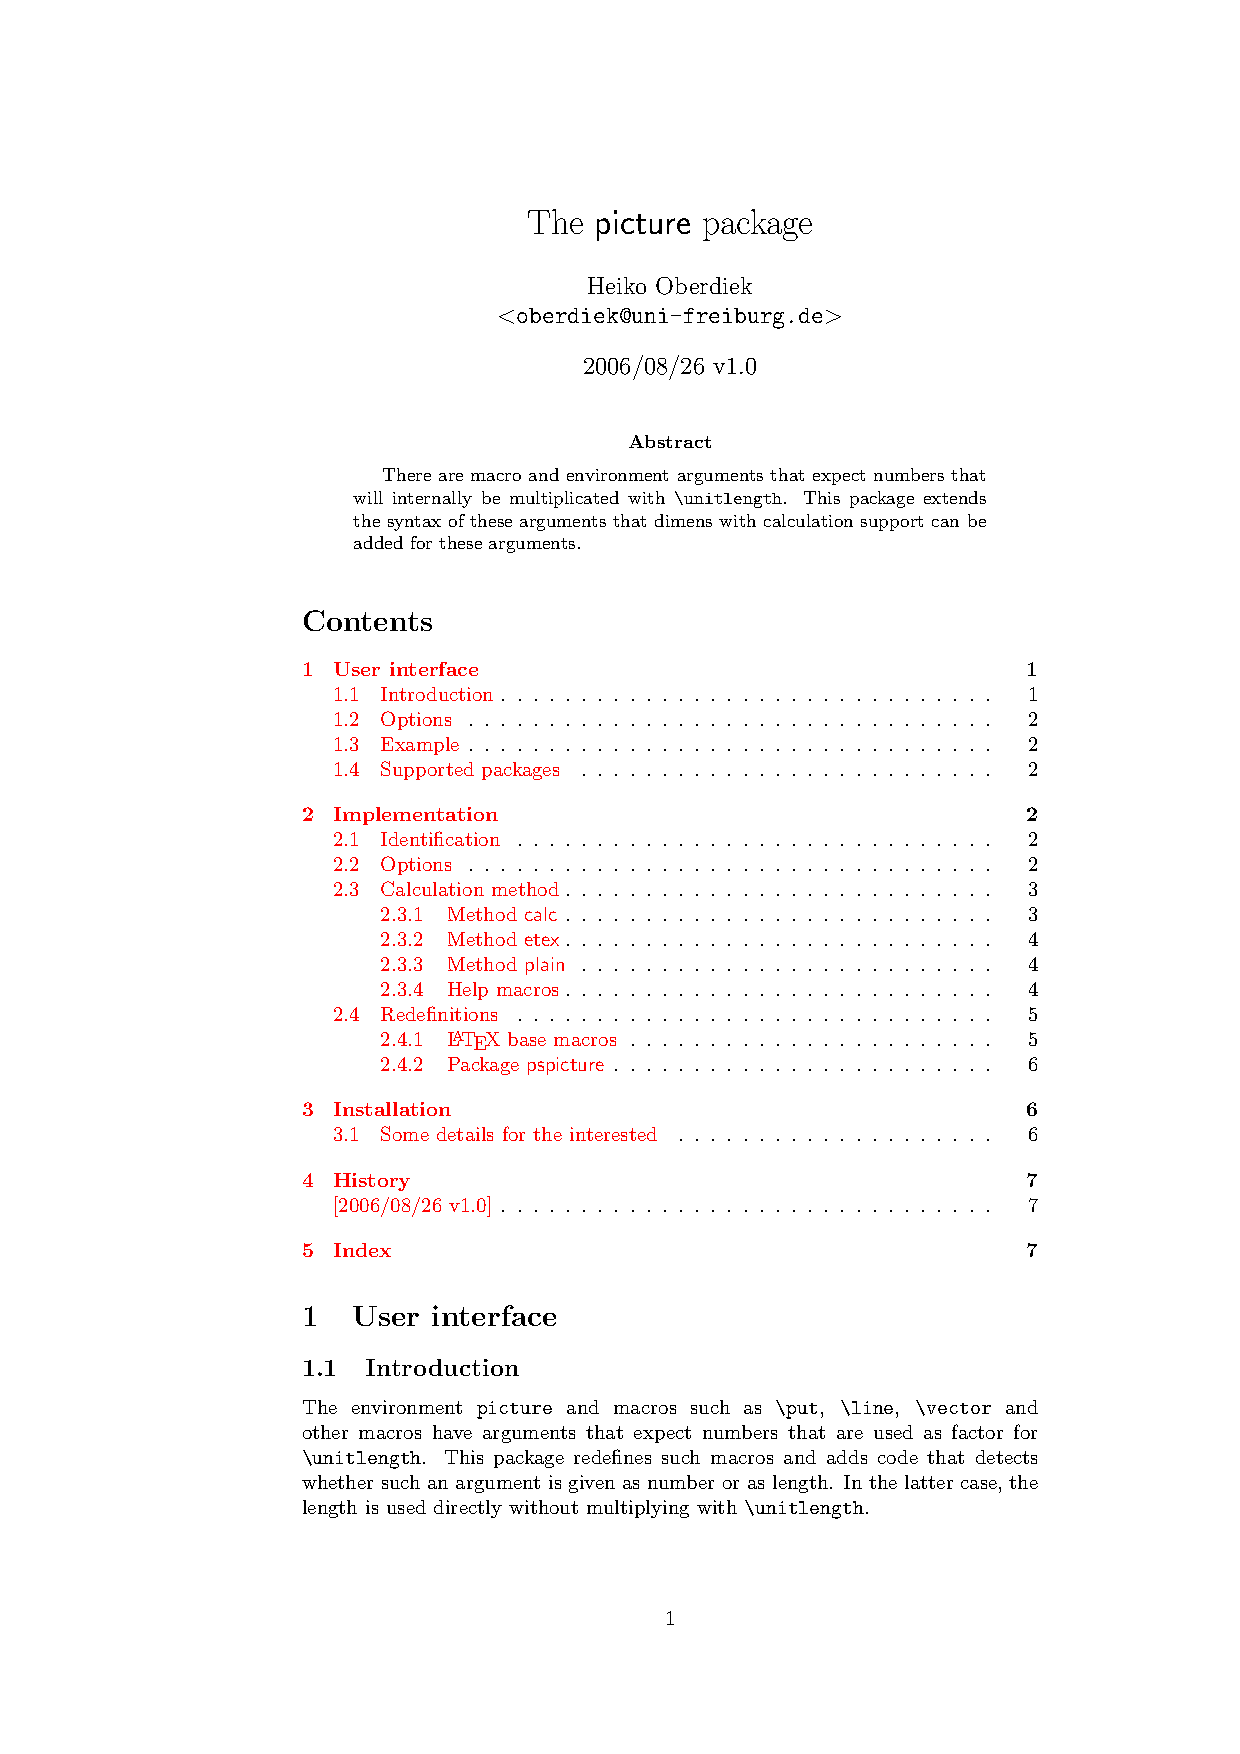
\includegraphics{picture}
\input{explanation}
\end{verbatim}
\end{quote}
then \cmdinvoke{import}{/home/friend/}{results} will include both
graph and explanation as one might hope.  A \csx{subimport} command
does the same sort of thing for a subdirectory (a relative path rather
than an absolute one), and there are corresponding \csx{includefrom}
and \csx{subincludefrom} commands.

The \Package{chapterfolder} package provides commands to deal with its
(fixed) model of file inclusion in a document.  It provides commands
\csx{cfpart}, \csx{cfchapter}, \csx{cfsection} and \csx{cfsubsection},
each of which takes directory and file arguments, e.g.:
\begin{quote}
\begin{verbatim}
\cfpart[pt 1]{Part One}{part1}{part}
\end{verbatim}
\end{quote}
which command will issue a `normal' command % ! line break
\cmdinvoke{part}[pt 1]{Part One} and then input the file
\File{part1/part.tex}, remembering that \File{part1/} is now the
``current folder''.  There are also commands of the form
\csx{cfpartstar} (which corresponds to a \csx{part*} command).

Once you're ``in'' a \Package{chapterfolder}-included document, you
may use \csx{cfinput} to input something relative to the ``current
folder'', or you may use \csx{input}, using \csx{cfcurrentfolder} to
provide a path to the file.  (There are also
\csx{cfcurrentfolderfigure} for a \path{figure/} subdirectory and
\csx{cfcurrentfolderlistings} for a \path{listings/} subdirectory.)

Documentation of \Package{chapterfolder} is in French, but the
\File{README} in the directory is in English.
\begin{ctanrefs}
\item[chapterfolder.sty]\CTANref{chapterfolder}
\item[import.sty]\CTANref{import}
\end{ctanrefs}

\Question[Q-RCS]{Version control using \acro{RCS}, \acro{CVS} or \ProgName{Subversion}}

If you use \acro{RCS}, \acro{CVS} or \ProgName{Subversion} to maintain
your \AllTeX{} documents under version control, you may need some
mechanism for including the version details in your document, in such
a way that they can be typeset (that is, rather than just hiding them
inside a comment).

The most complete solution for \acro{RCS} and \acro{CVS} is to use the
(\LaTeX{}) package \Package{rcs}, which allows you to parse and
display the contents of \acro{RCS} keyword fields in an extremely
flexible way.  The package \Package{rcsinfo} is simpler, but does most
of what you want, and some people prefer it; it is explicitly
compatible with \ProgName{LaTeX2HTML}.

If, however, you need a solution which works without using external
packages, or which will work in Plain \TeX{}, then you can use the
following minimal solution:
\begin{quote}
\begin{wideversion}
\begin{verbatim}
\def\RCS$#1: #2 ${\expandafter\def\csname RCS#1\endcsname{#2}}
\RCS$Revision: 1.426 $ % or any RCS keyword
\RCS$Date: 2006/12/18 09:59:16 $
...
\date{Revision \RCSRevision, \RCSDate}
\end{verbatim}
\end{wideversion}
\begin{narrowversion}
\begin{verbatim}
\def\RCS$#1: #2 ${\expandafter
  \def\csname RCS#1\endcsname{#2}%
}
\RCS$Revision: 1.426 $ % or any RCS keyword
\RCS$Date: 2006/12/18 09:59:16 $
...
\date{Revision \RCSRevision, \RCSDate}
\end{verbatim}
\end{narrowversion}
\end{quote}

If you've entered the brave new world of \ProgName{subversion}, the
package \Package{svn} may be for you.  It has explicit cleverness
about dealing with dates:
\begin{quote}
\csx{documentclass}\texttt{\{\meta{foo}\}}\\
\texttt{...}\\
\cmdinvoke{usepackage}{svn}\\
\csx{SVNdate}\texttt{ \$Date\$}\\
\cmdinvoke{author}{...}\\
\cmdinvoke{title}{...}\\
\texttt{...}\\
\cmdinvoke{begin}{document}\\
\csx{maketitle}\\
\texttt{...}\\
\cmdinvoke{end}{document}
\end{quote}
will (once \ProgName{subversion} has committed a copy of the document)
cause \csx{maketitle} use the date that has been written into the
\texttt{\$Date\$} keyword.

The alternative is the \Package{svninfo} package, which has much the
same mechanisms as does \Package{svn} but with a rather different
focus.  \Package{Svninfo} does the date trick that \Package{svn}
performs (controlled by a package option), and can set up page
foot-lines using \Qref*{package \Package{fancyhdr}}{Q-fancyhdr}.
There isn't much to choose between the two packages: you should read
the packages' documentation to see which you find best.
\begin{ctanrefs}
\item[rcs.sty]\CTANref{rcs}
\item[rcsinfo.sty]\CTANref{rcsinfo}
\item[svn.sty]\CTANref{svn}
\item[svninfo.sty]\CTANref{svninfo}
\end{ctanrefs}

\Question[Q-make]{Makefiles for \LaTeX{} documents}

\LaTeX{} is a tricky beast for running \ProgName{make} on: the need to
instruct \LaTeX{} to run several times for essentially different
reasons (for example, ``get the table of contents stable'', ``get the
labels stable'', ``add the bibliography'', ``add the index'') is
actually rather difficult to express in the `ordinary' sort of
dependency graph that one constructs for \ProgName{make}.

For this reason, the only \ProgName{make}-like package on \acro{CTAN}
(for a long time) was \ProgName{latexmk}, which is a \ProgName{Perl}
script that analyses your \LaTeX{} source for its dependencies, runs
\BibTeX{} or \ProgName{makeindex} as and when it notices that those
programs' input (parts of the |.aux| file, or the |.idx| file,
respectively) has changed, and so on.  \ProgName{Latexmk} is a fine
solution (and was used in generating printable versions of these
\acro{FAQ}s for a long time); it has recently been upgraded and has
many bells and whistles that allow it to operate as if it were a poor
man's \WYSIWYG{} system.

The \Qref*{\Package{texinfo} system}{Q-texinfo} comes with a
utility called \ProgName{texi2dvi}, which is capable of ``converting''
either \LaTeX{} or \Package{texinfo} files into \acro{DVI} (or into
\acro{PDF}, using \PDFTeX{}).

A later contribution is the bundle \Package{latexmake}, which
offers a set of \ProgName{make} rules that invoke \ProgName{texi2dvi}
as necessary.

The curious may examine the rules employed to run the present
\acro{FAQ} through \LaTeX{}: we don't present them as a complete
solution, but some of the tricks employed are surely re-usable.
\begin{ctanrefs}
\item[\nothtml{\rmfamily}\acro{FAQ} distribution]\CTANref{faq}
\item[\nothtml{\rmfamily}latexmake]\CTANref{latexmake}
\item[latexmk]\CTANref{latexmk}
\item[texi2dvi]Distributed as part of \CTANref{texinfo}
\end{ctanrefs}

\Question[Q-howmanypp]{How many pages are there in my document?}

Simple documents (those that start at page 1, and don't have any
breaks in their page numbering until their last page) present no
problem to the seeker after this truth.  The number of pages is
reported by the \Package{lastpage} package in its \texttt{LastPage} label.

For more complicated documents (most obviously, books with frontmatter
in a different series of page numbers) this simple approach will not
do.

The \Package{count1to} package defines a label \texttt{TotalPages}; this is
the value of its copy of \csx{count1} (a reserved \TeX{} count
register) at the end of the document.

Package \Package{totpages} defines a label \texttt{TotPages}, but it also
makes the register it uses available as a \LaTeX{} counter,
\texttt{TotPages}, which you can also reference via \csx{theTotPages}.  Of
course, the counter |TotPages| is asynchronous in the same way that
page numbers are, but snapshots may safely be taken in the output
routine.

The \Class{memoir} class defines two counters \texttt{lastpage} and
\texttt{lastsheet}, which are set (after the first run of a document)
to the equivalent of the \texttt{LastPage} label and the
\texttt{TotalPages} labels.

Both \Package{count1to} and \Package{totpages} need the support of
the \Package{everyshi} package.
\begin{ctanrefs}
\item[count1to.sty \nothtml{\bgroup\rmfamily}and\nothtml{\egroup} everyshi.sty]% line break!!
  Distributed in \CTANref{ms}
\item[lastpage.sty]\CTANref{lastpage}
\item[memoir.cls]\CTANref{memoir}
\item[totpages.sty]\CTANref{totpages}
\end{ctanrefs}

\Question[Q-inclplain]{Including Plain \TeX{} files in \LaTeX{}}

\LaTeX{}, though originally \nothtml{based on Plain \TeX{} (}% beware line brk
\Qref{based on Plain \TeX{}}{Q-LaTeXandPlain}\nothtml{)}, does not
contain all of Plain \TeX{}'s commands.  Worse, some Plain \TeX{}
command names appear in \LaTeX{}, with different semantics.  As a
result, special measures need to be taken to allow general Plain
\TeX{} documents (or parts of documents) to be typeset within
\LaTeX{}.

The truly reliable way is to translate the Plain \TeX{} commands, to
produce an equivalent of the original's semantics.  However, this is
not practical in many circumstances, and for those occasions, the
\Package{plain} package will often come to your aid.  The package
defines a \environment{plain} environment, in which a Plain \TeX{}
document may be processed:
\begin{quote}
\begin{verbatim}
\begin{plain}
  \input{plain-doc}
\end{plain}
\end{verbatim}
\end{quote}
The package is known to fail, for example, with documents that use
\AMSTeX{}; no doubt it would also fail if asked to load \Eplain{}.
All these things can be overcome (although it's not often easy), but
the environment saves a lot of work on many occasions.
\begin{ctanrefs}
\item[plain.sty]Distributed as part of \CTANref{carlisle}
\end{ctanrefs}

\subsection{Hyphenation}

\Question[Q-nohyph]{My words aren't being hyphenated}

Let's assume you've selected the right \TeX{} `language'~--- as
explained in \Qref[question]{``how hyphenation works''}{Q-hyphen},
you're not likely to get the correct results typesetting one language
using the hyphenation rules of another.  (Select the proper language,
using \Package{babel} if you're a \LaTeX{} user.  This may reveal that
you need another set of hyphenation patterns; see
% beware line wrap
\Qref[question]{``using a new language''}{Q-newlang} for advice on how
to install it.)

So what else can go wrong?
\begin{itemize}
\item Since \TeX{} version~3.0, the limits on how near to either end
  of a word hyphenation may take place have been programmable (see
  \Qref[question]{``weird hyphenation''}{Q-weirdhyphen}), and for some
  reason the values in question may have been corrupted in some macros
  you are using.  \TeX{} won't hyphenate less than \csx{lefthyphenmin}
  characters after the start of a word, nor less than
  \csx{righthyphenmin} before the end of a word; thus it won't
  hyphenate a word shorter than the sum of the two minima, at all.
  For example, since the minima are 2 and 3 for English, \TeX{} won't
  hyphenate a word shorter than 5 letters long, if it believes the
  word to be English.
\item \TeX{} won't hyphenate a word that's already been hyphenated.
  For example, the (caricature) English surname Smyth-Postlethwaite
  wouldn't hyphenate, which could be troublesome.  This is correct
  English typesetting style (it may not be correct for other
  languages), but if needs must, you can replace the hyphen in the
  name with a \csx{hyph} command, defined
\begin{quote}
\begin{verbatim}
\def\hyph{-\penalty0\hskip0pt\relax}
\end{verbatim}
\end{quote}
  This is \emph{not} the sort of thing this \acro{FAQ} would
  ordinarily recommend\dots{} The \Package{hyphenat} package defines a
  bundle of such commands (for introducing hyphenation points at
  various punctuation characters).
\item There may be accents in the word.  The causes of and remedies
  for this effect are discussed in
  % beware line break
  \Qref[question]{accents and hyphens}{Q-hyphenaccents}.
\item The hyphenation may simply not have been spotted; while \TeX{}'s
  algorithm is good, it's not infallible, and it does miss perfectly
  good hyphenations in some languages.  When this happens, you need to
  give \TeX{} \emph{explicit} instructions on how to hyphenate.
\end{itemize}
The \csx{hyphenation} command allows you to give explicit instructions.
Provided that the word will hyphenate at all (that is, it is not
prevented from hyphenating by any of the other restrictions above),
the command will override anything the hyphenation patterns might
dictate.  The command takes one or more hyphenated words as
argument~--- \cmdinvoke{hyphenation}{ana-lysis pot-able}; note that
(as here, for analysis) you can use the command to overrule \TeX{}'s
choice of hyphenation (ana-lysis is the British etymological
hyphenation; some feel the American hyphenation feels
`unfortunate'\dots{}).
\begin{ctanrefs}
\item[hyphenat.sty]\CTANref{hyphenat}
\end{ctanrefs}

\Question[Q-weirdhyphen]{Weird hyphenation of words}

If your words are being h-yphenated, like this, with jus-t single
letters at the 
beginning or the end of the word, you may have a version mismatch
problem. \TeX{}'s hyphenation system changed between version~2.9
and~3.0, and macros written for use with version~2.9 can have this
effect with a version~3.0 system.  If you are using Plain \TeX{}, make
sure your \File{plain.tex} file has a version number which is at
least~3.0, and rebuild your format.  If you are using \LaTeXo{} your
best plan is to upgrade to \LaTeXe{}.  If for some reason you can't,
the last version of \LaTeXo{} (released on 25 March 1992) is still
available (for the time being at least) and ought to solve this
problem.

If you're using \LaTeXe{}, the problem probably arises from your
|hyphen.cfg| file, which has to be created if you're using a
multi-lingual version.

A further source of oddity can derive from the 1995 release of
\Qref*{Cork-encoded fonts}{Q-ECfonts},
which introduced an alternative hyphen character.  The \LaTeXe{}
configuration files in the font release specified use of the
alternative hyphen, and this could produce odd effects with words
containing an explicit hyphen.  The font configuration files in the
December 1995 release of \LaTeXe{} do \emph{not} use the alternative
hyphen character, and therefore removed this source of problems; the
solution, again, is to upgrade your \LaTeX{}.
\begin{ctanrefs}
\item[\nothtml{\rmfamily}\LaTeXo{}]\CTANref{latex209-base}
\item[plain.tex]\CTANref{plain}
\end{ctanrefs}

\Question[Q-oddhyphen]{(Merely) peculiar hyphenation}

You may have found that \TeX{}'s famed automatic word-division does
not produce the break-points recommended by your dictionary. This may be
because \TeX{} is set up for American English, whose rules for word
division (as specified, for example, in Webster's Dictionary) are
completely different from the British ones (as specified, for example,
in the Oxford Dictionaries). This problem is being addressed by the \acro{UK}
\TeX{} User community (see \BV{}, issue~4.4) but an entirely
satisfactory solution will take time; the current status is to be
found on \acro{CTAN} (see
% beware line-wrap
\Qref[question]{``using a new language''}{Q-newlang} for instructions
on adding this new ``language'').
\begin{ctanrefs}
\item[UK patterns]\CTANref{ukhyph}
\end{ctanrefs}

\Question[Q-hyphenaccents]{Accented words aren't hyphenated}

\TeX{}'s algorithm for hyphenation gives up when it encounters an
\csx{accent} command; there are good reasons for this, but it means
that quality typesetting in non-English languages can be difficult.

For \TeX{} macro packages, you can avoiding the effect by using an
appropriately encoded font (for example, a Cork-encoded font~--- see
\Qref[question]{the \acro{EC} fonts}{Q-ECfonts}) which contains accented
letters as single glyphs.  \LaTeX{} users can achieve this end simply
by adding the command
\begin{verbatim}
  \usepackage[T1]{fontenc}
\end{verbatim}
to the preamble of their document.  Other encodings (notably
\acro{LY}1, once promoted by \YandY{} inc) may be used
in place of \acro{T}1.  Indeed, most current 8-bit \TeX{} font
encodings will `work' with the relevant sets of hyphenation patterns. 

One might hope that, with the many aspirant successors to \TeX{} such
as
\begin{wideversion}
  \Qref{Omega}{Q-omegaleph}, \Qref{\acro{LUA}\TeX{}}{Q-luatex} and
  \Qref{Ex\TeX{}}{Q-extex},
\end{wideversion}
\begin{narrowversion}
  Omega, \acro{LUA}\TeX{} and Ex\TeX{}
  (\Qref[see questions]{}{Q-omegaleph}\Qref[,]{}{Q-luatex}
  \Qref[and]{}{Q-extex}),
\end{narrowversion}
all of which base their operations on Unicode, that the whole basis of
encodings will change.

\Question[Q-newlang]{Using a new language with Babel}

\Package{Babel} is capable of working with a large range of
languages, and a new user often wants to use a language that her
\TeX{} installation is not set up to employ.  Simply asking Babel to
use the language, with the command
\begin{verbatim}
  \usepackage[catalan]{babel}
\end{verbatim}
provokes the warning message
\begin{wideversion}
\begin{verbatim}
Package babel Warning: No hyphenation patterns were loaded for
(babel)                the language `Catalan'
(babel)                I will use the patterns loaded for \language=0 instead.
\end{verbatim}
\end{wideversion}
\begin{narrowversion}
\begin{verbatim}
Package babel Warning: No hyphenation patterns
                                 were loaded for
(babel)                the language `Catalan'
(babel)                I will use the patterns
                 loaded for \language=0 instead.
\end{verbatim}
(The first and third lines above have been wrapped to fit in the
column.)
\end{narrowversion}

The problem is that your \TeX{} system doesn't know how to hyphenate
Catalan text: you need to tell it how before Babel can do its work
properly.  To do this, for \LaTeX{} installations, one needs to change
\File{language.dat} (which is part of the Babel installation); it will
contain a line
\begin{verbatim}
%catalan         cahyphen.tex
\end{verbatim}
which, if you remove the comment marker, is supposed to instruct
\LaTeX{} to load Catalan hyphenation patterns when you tell it to build
a new format.

Unfortunately, in many Babel distributions, the line just isn't
right~--- you need to check the name of the file containing the
patterns you're going to use.  As you can see, in the author's system,
the name is supposed to be \File{cahyphen.tex}; however the file
actually present on the system is \File{cahyph.tex}~--- fortunately,
the error should prove little more than an inconvenience (most of the
files are in better distributions anyway, but an elusive one
may be found on \acro{CTAN}; if you have to retrieve
a new file, ensure that it's correctly installed, for which see
\Qref[question]{installing a new package}{Q-instpackages}).

Finally, you need to regenerate the formats used (in fact, most users
of Babel are using it in their \LaTeX{} documents, so regenerating the
\LaTeX{}-related formats will ordinarily be enough; however, the
author always generates the lot, regardless).
\begin{description}
\item[te\TeX{}]It's possible to do the whole operation in one go, by
  using the \ProgName{texconfig} command:
\begin{verbatim}
texconfig hyphen latex
\end{verbatim}
  which first enters an editor for you to edit \File{language.dat},
  and then regenerates the format you specify (\ProgName{latex} in
  this case).

  Otherwise, to regenerate all formats, do: \\
  \texttt{fmtutil -\relax-all}
  
  If you're willing to think through what you're doing (this is
  \emph{not} for the faint-hearted), you can select a sequence of
  formats and for each one, run: \\
  \texttt{fmtutil -\relax-byfmt \meta{formatname}}\\
  where \emph{\texttt{formatname}} is something like `\texttt{latex}',
  or: \\
  \texttt{fmtutil -\relax-byhyphen \meta{hyphenfile}}\\
  where \emph{\texttt{hyphenfile}} is the file specifying hyphenation
  to the format~--- usually \texttt{language.dat}
\item[\miktex{}] On a \Package{\miktex{}} distribution earlier than v2.0, do: \\
  \texttt{Start}\arrowhyph{}%
  \texttt{Programs}\arrowhyph{}%
  \texttt{\miktex{}}\arrowhyph{}%
  \texttt{Maintenance}\arrowhyph{}%
  \texttt{Create all format files}
% this sequence suggested for miktex 1.20e, 2000/12/22, by Giuseppe Bilotta

  or get a DOS window and run:\\
  \texttt{initexmf -\relax-dump}
  
  On a \Package{\miktex{}} distribtution v2.0 or later, the whole
  procedure can be done via the \acro{GUI}.  To select the new
  language, do:\\
  \texttt{Start}\arrowhyph{}%
  \texttt{Programs}\arrowhyph{}%
  \texttt{\miktex{} 2}\arrowhyph{}%
  \texttt{\miktex{} Options}, and select the \texttt{Languages} tab.
  Select your language from the list, press the \texttt{Apply} button,
  and then the \texttt{OK} button.  Then select the \texttt{General}
  tab and press the \texttt{Update Now} button.
  
  Otherwise, edit the \File{language.dat} file (as outlined above),
  and then run:\\
  \texttt{initexmf -\relax-dump}\\
  just as for a pre-v2.0 system.
\end{description}

\nothtml{\noindent}\textbf{\emph{Caveat}:} It is (just) possible that
your \TeX{} system may run out of ``pattern memory'' while generating
the new format.  Most \TeX{} implementations have fixed-size arrays
for storing the details of hyphenation patterns, but although their
size is adjustable in most modern distributions, actually changing the
size is a fiddle.  If you \emph{do} find you've run out of memory,
it may be worth scanning the list of languages in your
\File{language.dat} to see whether any could reasonably be removed.
\begin{ctanrefs}
\item[babel]\CTANref{babel}
\item[hyphenation patterns]\CTANref{hyphenation}
\end{ctanrefs}

\Question[Q-hyphoff]{Stopping all hyphenation}

It may seem an odd thing to want to do (after all, one of \TeX{}'s
great advertised virtues is the quality of its hyphenation) but it's
sometimes necessary.  The real problem is, that the quality of
\TeX{}'s output is by default largely dependent on the presence of
hyphenation; if you want to abandon hyphenation, something has to
give.

\TeX{} (slightly confusingly) offers four possible mechanisms for
suppressing hyphenation (there were only two prior to the extensions
that arrived with \TeX{} version~3).

First, one can set the hyphenation penalties \csx{hyphenpenalty} and
\csx{exhyphenpenalty} to an `infinite' value (that is to say, 10000).
This means that all hyphenations will sufficiently penalise the line
that would contain them, that the hyphenation won't happen.  The
disadvantage of this method is that \TeX{} will re-evaluate any
paragraph for which hyphenations might help, which will slow \TeX{}
down.

Second, one can select a language for which no hyphenation patterns
exist.  Some distributions create a language |nohyphenation|,
and the \Package{hyphenat} package uses this technique for its
\csx{nohyphens} command which sets its argument without any
hyphenation.

Third, one can set \csx{left-} and/or \csx{righthyphenmin} to a
sufficiently large value that no hyphenation could possibly succeed,
since the minimum is larger than the length of the longest word
\TeX{} is willing to hyphenate (the appropriate value is 62).

Fourth, one can suppress hyphenation for all text using the current
font by the command
\begin{quote}
\begin{verbatim}
\hyphenchar\font=-1
\end{verbatim}
\end{quote}
This isn't a particularly practical way for users to suppress
hyphenation~--- the command has to be issued for every font the
document uses~--- but it's how \LaTeX{} itself suppresses hyphenation
in \texttt{tt} and other fixed-width fonts.

Which of the techniques you should use depends on what you actually
want to do.  If the text whose hyphenation is to be suppressed runs
for less than a paragraph, your only choice is the no-hyphens
language: the language value is preserved along with the text (in the
same way that the current font is); the values for penalties and
hyphen minima active at the end of a paragraph are used when
hyphenation is calculated.

Contrariwise, if you are writing a multilanguage document using the
\Package{babel} package, you \emph{cannot} suppress hyphenation
throughout using either the no-hyphens language or the hyphen minima:
all those values get changed at a \Package{babel} language switch: use
the penalties instead.

If you simply switch off hyphenation for a good bit of text, the
output will have a jagged edge (with many lines seriously overfull),
and your \AllTeX{} run will bombard you with warnings about overfull
and underfull lines.  To avoid this you have two options.  You may use
\csx{sloppy} (or its environment version \environment{sloppypar}), and
have \TeX{} stretch what would otherwise be underfull lines to fill the space
offered, and wrap other lines, while prematurely wrapping overfull
lines and stretching the remainder.  Alternatively, you may set the
text \Qref*{ragged right}{Q-ragright}, and at least get rid of
the overfull lines; this technique is `traditional' (in the sense that
typists do it) and may be expected to appeal to the specifiers of
eccentric document layouts (such as those for dissertations), but for
once their sense conforms with typographic style.  (Or at least, style
constrained in this curious way.)
\begin{ctanrefs}
\item[hyphenat.sty]\CTANref{hyphenat}
\end{ctanrefs}

\Question[Q-wdnohyph]{Preventing hyphenation of a particular word}

It's quite possible for (\emph{any}) hyphenation of a particular word
to seem ``completely wrong'', so that you want to prevent it being
hyphenated.

If the word occurs in just one place, put it in a box:
\begin{quote}
\begin{verbatim}
\mbox{oddword}
\end{verbatim}
\end{quote}
(Plain~\TeX{} users should use \csx{hbox}, and take care at the start
of paragraphs.)  However, boxing the word is not really advisable
unless you are sure it only occurs once.

If the word occurs commonly, the best choice is to assert a
non-hyphenation for it:
\begin{quote}
\begin{verbatim}
\hyphenation{oddword}
\end{verbatim}
\end{quote}
This hyphenation exception (with no break points) will be used in
preference to what \TeX{}'s hyphenation algorithm may come up with.

In a multilingual document, repeat the exception specification for
each language the word may appear in.  So:
\begin{quote}
\begin{verbatim}
\usepackage[french,english]{babel}
\selectlanguage{english}
\hyphenation{oddword}
\selectlanguage{french}
\hyphenation{oddword}
\end{verbatim}
\end{quote}
(note that \Package{babel} will select the default language for the
document~--- English, in this case~--- at \cmdinvoke{begin}{document}.)

\Question[Q-hyphexcept]{Hyphenation exceptions}

While \TeX{}'s hyphenation rules are good, they're not infallible: you
will occasionally find words \TeX{} just gets \emph{wrong}.  So for
example, \TeX{}'s default hyphenation rules (for American English) don't
know the word ``\emph{manuscript}'', and since it's a long word you
may find you need to hyphenate it.  You \emph{can} ``write the
hyphenation out'' each time you use the word:
\begin{quote}
\begin{verbatim}
... man\-u\-script ...
\end{verbatim}
\end{quote}
Here, each of the \csx{-} commands is converted to a hyphenated break,
if (\emph{and only if}) necessary.

That technique can rapidly become tedious: you'll probably only accept
it if there are no more than one or two wrongly-hyphenated words in
your document.  The alternative is to set up hyphenations in the
document preamble.  To do that, for the hyphenation above, you would
write:
\begin{quote}
\begin{verbatim}
\hyphenation{man-u-script}
\end{verbatim}
\end{quote}
and the hyphenation would be set for the whole document.  Barbara
Beeton publishes articles containing lists of these ``hyphenation
exceptions'', in \textsl{TUGboat}; the hyphenation `man-u-script'
comes from one of those articles.

What if you have more than one language in your document?  Simple:
select the appropriate language, and do the same as above:
\begin{quote}
\begin{verbatim}
\usepackage[french]{babel}
\selectlanguage{french}
\hyphenation{re-cher-cher}
\end{verbatim}
\end{quote}
(nothing clever here: this is the ``correct'' hyphenation of the word,
in the current tables).  However, there's a problem here: just as
words with accents in them won't break, so \csx{hyphenation} commands
with accents in them produce an error:
\begin{quote}
\begin{verbatim}
\usepackage[french]{babel}
\selectlanguage{french}
\hyphenation{r\'e-f\'e-rence}
\end{verbatim}
\end{quote}
tells us that the hyphenation is ``improper'', and that it will be ``flushed''.
But, just as hyphenation of words is enabled by selecting an 8-bit
font encoding, so \csx{hyphenation} commands are rendered proper again
by selecting that same 8-bit font encoding.  For the hyphenation
patterns provided in the usual distributions, the encoding is
\Qref*{Cork}{Q-ECfonts}, so the complete sequence is:
\begin{quote}
\begin{verbatim}
\usepackage[T1]{fontenc}
\usepackage[french]{babel}
\selectlanguage{french}
\hyphenation{r\'e-f\'e-rence}
\end{verbatim}
\end{quote}

The same sort of performance goes for any language for which 8-bit
fonts and corresponding hyphenation patterns are available.  Since you
have to select both the language and the font encoding to have your
document typeset correctly, it should not be a great imposition to do
the selections before setting up hyphenation exceptions.

\subsection{Odds and ends}

\Question[Q-logos]{Typesetting all those \TeX{}-related logos}

Knuth was making a particular point about the capabilities of \TeX{}
when he defined the logo.  Unfortunately, many believe, he thereby
opened floodgates to give the world a whole range of rather silly
`bumpy road' logos such as \AMSTeX{}, \PiCTeX{}, \BibTeX{}, and so on,
produced in a flurry of different fonts, sizes, and baselines~--- indeed,
everything one might hope to cause them to obstruct the reading process.
In particular, Lamport invented \LaTeX{}
\htmlignore
(silly enough in itself)
\endhtmlignore
\begin{htmlversion}
  (silly enough in itself, with a raised small `A' and a lowered `E')
\end{htmlversion}
and marketing input from Addison-Wesley led to the even
stranger current logo
\htmlignore
\LaTeXe{}.
\endhtmlignore
\begin{htmlversion}
  \LaTeXe{}, which appends a lowered single-stroke Greek letter
  epsilon.
\end{htmlversion}

Sensible users don't have to follow this stuff wherever it goes,
but, for those who insist, a large collection of logos is defined in
the \Package{texnames} package (but note that this set of macros isn't
entirely reliable in \LaTeXe{}).
The \MF{} and \MP{} logos can be set in fonts that \LaTeXe{}
knows about (so that they scale with the surrounding text) using the
\Package{mflogo} package; but be aware that booby-traps surround the
use of the Knuthian font for \MP{} (you might get
\htmlignore
\textlogo{META\hphantom{P}O\hphantom{S}T}).
\endhtmlignore
% the following htmlversion stuff seems to do roughly what's required,
% which is nice, given the feebleness of representing all these silly
% logos in html otherwise...
\begin{htmlversion}
  something like `META&nbsp;O&nbsp;T').
\end{htmlversion}
You needn't despair, however~--- the author himself uses just `MetaPost'.

For those who don't wish to acquire the `proper' logos, the canonical
thing to do is to say \texttt{AMS-}\cmdinvoke{TeX}{}
\htmlignore
(\acro{AMS}-\TeX{})
\endhtmlignore
for \AMSTeX{}, \texttt{Pic}\cmdinvoke{TeX}{}
\htmlignore
(Pic\TeX{})
\endhtmlignore
for \PiCTeX{}, \texttt{Bib}\cmdinvoke{TeX}{}
\htmlignore
(Bib\TeX{})
\endhtmlignore
for \BibTeX{}, and so on.
\begin{ctanrefs}
\item[mflogo.sty]\CTANref{mflogo}
\item[texnames.sty]\CTANref{texnames}
\end{ctanrefs}

\Question[Q-bold-extras]{How to do bold-tt or bold-sc}

\LaTeX{}, as delivered, offers no means of handling bold ``teletype''
or small-caps fonts.  There's a practical reason for this (Knuth never
designed such fonts), but there are typographical considerations too
(the ``medium weight'' \texttt{cmtt} font is already pretty bold (by
comparison with other fixed-width fonts), and bold small-caps is not
popular with many professional typographers).

There's a set of ``extra'' \MF{} files on \acro{CTAN} that provide bold
versions of both \texttt{cmtt} and \texttt{cmcsc} (the small caps font).  With
modern \TeX{} distributions, one may bring these fonts into use simply
by placing them in an % ! line break
\Qref*{appropriate place in the \emph{texmf} tree}{Q-wherefiles}
(these are \AllTeX{}-specific files, so the ``\emph{public}'' supplier
would be an appropriate place).  Once you've % ! line break, again
\Qref*{rebuilt the file indexes as necessary}{Q-instpackages},
\TeX{} (and friends) will automatically build whatever font files they
need when you first make reference to them.  There's a jiffy package
\Package{bold-extra} that builds the necessary font data structures
so that you can use the fonts within \LaTeX{}.

Another alternative is to use the \Qref*{\acro{EC} fonts}{Q-ECfonts},
which come with bold variants of the small-caps fonts.

If you need to use Type~1 fonts, you can't proceed with Knuth-style
fonts, since there are no Type~1 versions of the \Package{mf-extra}
set.  There are, however, Type~1 distributions of the EC~fonts, so you
can switch to EC and use them; alternatives are discussed in
\Qref[question]{8-bit Type~1 fonts}{Q-type1T1}.

Of course, commercial fixed-width fonts (even the default
\FontName{Courier}) almost always come with a bold variant, so that's
not a problem.  Furthermore \Qref*{\acro{PSNFSS}}{Q-usepsfont}
will usually provide ``faked'' small caps fonts, and has no
compunctions about providing them in a bold form.  \FontName{Courier}
is (as we all know, to our cost) freely available; a far more
presentable monospace font is \FontName{LuxiMono}, which is also
freely available (monospace text in the typeset version of this
\acro{FAQ} uses \FontName{LuxiMono}, with the metrics and \LaTeX{}
support available on the archive.
\begin{ctanrefs}
\item[bold-extra.sty]\CTANref{bold-extra}
\item[bold tt and small caps fonts]\CTANref{bold}
\item[\nothtml{rmfamily}LuxiMono fonts]\CTANref{luximono}
\end{ctanrefs}

\Question[Q-varwidth]{Automatic sizing of \environment{minipage}}

The \environment{minipage} environment requires you to specify the
width of the ``page'' you're going to create.  This is sometimes
inconvenient: you would like to occupy less space, if possible, but
\environment{minipage} sets a box that is exactly the width you
specified.

The \Package{pbox} package defines a \csx{pbox} whose width is exactly
that of the longest enclosed line, subject to a maximum width that you
give it.  So while \cmdinvoke{parbox}{2cm}{Hello\bsbs world!} produces a
box of width exactly \texttt{2cm},
\cmdinvoke{pbox}{2cm}{Hello\bsbs world!} produces one whose width is
\texttt{1.79cm} (if one's using the default \FontName{cmr} font for the
text, at least).  The package also provides a
\cmdinvoke*{settominwidth}[min]{length}{text} (which looks (almost)
like the standard \csx{settowidth} command), and a \csx{widthofpbox}
function analagous to the \csx{widthof} command for use with the
\Package{calc} package.

The \Package{eqparbox} package extends \Package{pbox}'s idea, by
allowing you to set a series of boxes, all with the same (minimised)
width.  (Note that it doesn't accept a limiting maximum width
parameter.)  The package documentation shows the following example
drawn from a joke \emph{curriculum vitae}:
\begin{quote}
\begin{narrowversion}
\begin{verbatim}
\noindent%
\eqparbox{place}%
    {\textbf{Widgets, Inc.}}
        \hfill
\eqparbox{title}%
    {\textbf{Senior Widget Designer}}
        \hfill
\eqparbox{dates}{\textbf{1/95--present}}

...

\noindent%
\eqparbox{place}%
    {\textbf{Thingamabobs, Ltd.}}
        \hfill
\eqparbox{title}%
    {\textbf{Lead Engineer}}
        \hfill
\eqparbox{dates}{\textbf{9/92--12/94}}
\end{verbatim}
\end{narrowversion}
\begin{wideversion}
\begin{verbatim}
\noindent%
\eqparbox{place}{\textbf{Widgets, Inc.}} \hfill
\eqparbox{title}{\textbf{Senior Widget Designer}} \hfill
\eqparbox{dates}{\textbf{1/95--present}}

...

\noindent%
\eqparbox{place}{\textbf{Thingamabobs, Ltd.}} \hfill
\eqparbox{title}{\textbf{Lead Engineer}} \hfill
\eqparbox{dates}{\textbf{9/92--12/94}}
\end{verbatim}
\end{wideversion}
\end{quote}
The code makes the three items on each of the heading lines have
exactly the same width, so that the lines as a whole produce a regular
pattern down the page.  A command \csx{eqboxwidth} allows you to use
the measured width of a group: the documentation shows how the command
may be used to produce sensible-looking columns that mix \texttt{c}-,
\texttt{r}- or \texttt{l}-rows, with the equivalent of a |p{...}|
entry, by making the fixed-width rows an \Package{eqparbox} group, and
making the last from a \csx{parbox} using the width that's been
measured for the group.

The \Package{varwidth} package defines a \environment{varwidth}
environment which sets the content of the box to match a ``narrower
natural width'' if it finds one.  (You give it the same parameters as
you would give \environment{minipage}: in effect, it is a `drop-in'
replacement.)  \Package{Varwidth} provides its own ragged text command:
\csx{narrowragged}, which aims to make narrower lines and to put more
text in the last line of the paragraph (thus producing lines with more
nearly equal lengths than typically happens with \csx{raggedright}
itself).

The documentation (in the package file) lists various restrictions and
things still to be done, but the package is already proving useful for
a variety of jobs.
\begin{ctanrefs}
\item[eqparbox.sty]\CTANref{eqparbox}
\item[pbox.sty]\CTANref{pbox}
\item[varwidth.sty]\CTANref{varwidth}
\end{ctanrefs}

%%%%%%%%%%%%%%%%%%%%%%%%%%%%%%%%%%%%%%%%%%%%%%%%%%%%%%%%%%%%%%%%%

\section{Symbols, etc.}

\Question[Q-numbersets]{Symbols for the number sets}

It is a good idea to have commands such as \csx{R} for the real numbers and
other standard number sets. Traditionally these were typeset in bold.
Because, in the ordinary course of events, mathematicians do not have
access to bold chalk, they invented the special symbols that are now
often used for \csx{R}, \csx{C}, \emph{etc}.  These symbols are known
as ``blackboard bold''.  Before insisting on using them, consider
whether going back to the old system of ordinary bold might not be
acceptable (it is certainly simpler).

A set of blackboard bold capitals is available in the \acro{AMS}
\FontName{msbm} fonts (\FontName{msbm} is available at a range of
design sizes, with names such as \FontName{msbm10}). The pair of font
families (the other is called \FontName{msam}) have a large number of
mathematical symbols to supplement the ones in the standard \TeX{}
distribution, and are available in Type~1 format with most modern
distributions. Support files for using the fonts, both under
Plain~\TeX{} and \LaTeX{} (packages \Package{amssymb} and
\Package{amsfonts}), are available.  The font shape is a rather
austere sans, which many people don't like (though it captures the
essence of quickly-chalked writing rather well).

The \FontName{bbold} family is set of blackboard bold fonts written in
\MF{}.  This set offers blackboard bold forms of lower-case letters;
the font source directory also contains sources for a \LaTeX{} package
that enables use of the fonts.  The fonts are not available in Type~1 format.

The \FontName{bbm} family claims to provide
`blackboard' versions of most of the \FontName{cm} fonts~\dots{} including
the bold and bold-extended series.  Again, the fonts are designed in
\MF{} and are not available in Type~1 format.  \LaTeX{} macro support
comes from a package by Torsten Hilbrich.

The \FontName{doublestroke} family comes in just roman
and sans shapes, at a single weight, and is available both as \MF{}
sources and as Type~1; the font covers the uppercase latin letters,
lowercase `h' and 'k', and the digit `1'.

An alternative source of Type~1 fonts with blackboard bold characters
may be found in the steadily increasing set of complete families, both
commercial and free, that have been prepared for use with \AllTeX{}
(see % beware line break
\htmlonly{``}\Qref[question]{choice of outline fonts}{Q-psfchoice}\htmlonly{''}).
Of the free sets, the \FontName{txfonts} and \FontName{pxfonts} families
both come with replicas of \FontName{msam} and \FontName{msbm}
(though, as noted elsewhere, there are other reasons not to use these
fonts).  The \FontName{mathpazo} family includes a ``mathematically
significant'' choice of blackboard bold characters, and the
\FontName{fourier} fonts contain blackboard bold upper-case letters,
the digit `1', and lower-case `k'.

The ``lazy person's'' blackboard bold macros:
\begin{quote}
\begin{verbatim}
\newcommand{\R}{{\sf R\hspace*{-0.9ex}%
  \rule{0.15ex}{1.5ex}\hspace*{0.9ex}}}
\newcommand{\N}{{\sf N\hspace*{-1.0ex}%
  \rule{0.15ex}{1.3ex}\hspace*{1.0ex}}}
\newcommand{\Q}{{\sf Q\hspace*{-1.1ex}%
  \rule{0.15ex}{1.5ex}\hspace*{1.1ex}}}
\newcommand{\C}{{\sf C\hspace*{-0.9ex}%
  \rule{0.15ex}{1.3ex}\hspace*{0.9ex}}}
\end{verbatim}
\end{quote}
are almost acceptable at normal size if the surrounding text is
\FontName{cmr10}.  However, they are not part of a proper maths font,
and so do not work in sub- and superscripts.  Moreover, the size and
position of the vertical bar can be affected by the font of the
surrounding text.  As we've seen, there are plenty of alternatives:
don't try the macros, or anything similar using capital `I' (which
looks even worse!).
\begin{ctanrefs}
\item[AMS support files (Plain)]\CTANref{amsfonts-plain}
\item[AMS support files (LaTeX)]\CTANref{amsfonts-latex}
\item[AMS symbol fonts]\CTANref{amsfonts-symbols}
\item[AMS symbol fonts in Type~1 format]Browse \CTANref{ams-AMStype1}
\item[bbm fonts]\CTANref{bbm}
\item[bbm macros]\CTANref{bbm-macros}
\item[bbold fonts]\CTANref{bbold}
\item[doublestroke fonts]\CTANref{doublestroke}
\item[fourier fonts]\CTANref{fourier}
\item[mathpazo fonts]\CTANref{mathpazo}
\item[pxfonts]\CTANref{pxfonts}
\item[txfonts]\CTANref{txfonts}
\end{ctanrefs}

\Question[Q-scriptfonts]{Better script fonts for maths}

The font selected by \csx{mathcal} is the only script font `built
in'. However, there are other useful calligraphic fonts included with
modern \TeX{} distributions.
\begin{description}
\item[Euler] The \Package{eucal} package (part of most sensible \TeX{}
  distributions; the fonts are part of the \acro{AMS} font set) gives
  a slightly curlier font than the default. The package changes the
  font that is selected by \csx{mathcal}.
  
  Type 1 versions of the fonts are available in the \acro{AMS} fonts
  distribution.
\item[RSFS] The \Package{mathrsfs} package uses a really fancy script
  font (the name stands for ``Ralph Smith's Formal Script'') which is
  already part of most modern \TeX{} distributions.  The package
  creates a new command \csx{mathscr}.
  
  Type 1 versions of the font have been made available by Taco
  Hoekwater.
\item[Zapf Chancery] is the standard \PS{} calligraphic font.  There
  is no package but you can easily make it available by means of the
  command
\begin{verbatim}
\DeclareMathAlphabet{\mathscr}{OT1}{pzc}%
                                 {m}{it}
\end{verbatim}
  in your preamble.  You may find the font rather too big; if so, you
  can use a scaled version of it like this:
\begin{verbatim}
\DeclareFontFamily{OT1}{pzc}{}
\DeclareFontShape{OT1}{pzc}{m}{it}%
             {<-> s * [0.900] pzcmi7t}{}
\DeclareMathAlphabet{\mathscr}{OT1}{pzc}%
                                 {m}{it}
\end{verbatim}
  
  Adobe Zapf Chancery (which the above examples use) is distributed in
  any but the most basic \PS{} printers.  A substantially identical
  font (to the extent that the same metrics may be used) is
  available from \acro{URW} and is distributed with
  \ProgName{ghostscript}.
\end{description}
Examples of the available styles are available on \acro{CTAN}.
\begin{ctanrefs}
\item[eucal.sty]\CTANref{eucal}
\item[euler fonts]\CTANref{amsfonts-euler}
\item[euler fonts, in Type 1 format]\CTANref{ams-AMStype1}
\item[ghostscript]Browse \CTANref{ghostscript}
\item[mathrsfs.sty]Distributed as part of \CTANref{jknappen-macros}
\item[rsfs fonts]\CTANref{rsfs}
\item[rsfs fonts, in Type 1 format]\CTANref{rsfs-type1}
\item[Script font examples]\CTANref{mathscript}
\end{ctanrefs}

\Question[Q-boldgreek]{Setting bold Greek letters in \LaTeX{}}

The issue here is complicated by the fact that \csx{mathbf} (the
command for setting bold \emph{text} in \TeX{} maths) affects a select
few mathematical symbols (the uppercase Greek letters).  However
lower-case Greek letters behave differently from upper-case Greek
letters (due to Knuth's esoteric font encoding decisions).  However,
\csx{mathbf} \emph{can't} be used even for upper-case Greek letters in
the \AMSLaTeX{} \Package{amsmath} package, which
disables this font-switching and you must use one of the techniques
outlined below.

The Plain \TeX{} solution \emph{does} work, in a limited way:
\begin{quote}
\begin{verbatim}
{\boldmath$\theta$}
\end{verbatim}
\end{quote}
but \csx{boldmath} may not be used in maths mode, so this `solution'
requires arcana such as:
\begin{quote}
\begin{verbatim}
$... \mbox{\boldmath$\theta$} ...$
\end{verbatim}
\end{quote}
which then causes problems in superscripts, etc.

These problems may be addressed by using a bold mathematics package.
\begin{itemize}
\item The \Package{bm} package, which is part of the \LaTeX{} tools
  distribution, defines a command \csx{bm} which may be used anywhere
  in maths mode.
\item The \Package{amsbsy} package (which is part of \AMSLaTeX{})
  defines a command \csx{boldsymbol}, which (though slightly less
  comprehensive than \csx{bm}) covers almost all common cases.
\end{itemize}

All these solutions cover all mathematical symbols, not merely Greek
letters.
\begin{ctanrefs}
\item[bm.sty]Distributed as part of \CTANref{2etools}
\item[amsbsy.sty]Distributed as part of \AMSLaTeX{} \CTANref{amslatex}
\item[amsmath.sty]Distributed as part of \AMSLaTeX{}
  \CTANref{amslatex}
\end{ctanrefs}

\Question[Q-prinvalint]{The Principal Value Integral symbol}

This symbol (an integral sign, `crossed') does not appear in any of
the fonts ordinarily available to \AllTeX{} users, but it can be
created by use of the following macros:
\begin{wideversion}
\begin{verbatim}
\def\Xint#1{\mathchoice
   {\XXint\displaystyle\textstyle{#1}}%
   {\XXint\textstyle\scriptstyle{#1}}%
   {\XXint\scriptstyle\scriptscriptstyle{#1}}%
   {\XXint\scriptscriptstyle\scriptscriptstyle{#1}}%
   \!\int}
\def\XXint#1#2#3{{\setbox0=\hbox{$#1{#2#3}{\int}$}
     \vcenter{\hbox{$#2#3$}}\kern-.5\wd0}}
\def\ddashint{\Xint=}
\def\dashint{\Xint-}
\end{verbatim}
\end{wideversion}
\begin{narrowversion}
\begin{verbatim}
\def\Xint#1{\mathchoice
   {\XXint\displaystyle\textstyle{#1}}%
   {\XXint\textstyle\scriptstyle{#1}}%
   {\XXint\scriptstyle\scriptscriptstyle{#1}}%
   {\XXint\scriptscriptstyle
                      \scriptscriptstyle{#1}}%
   \!\int}
\def\XXint#1#2#3{{%
     \setbox0=\hbox{$#1{#2#3}{\int}$}
     \vcenter{\hbox{$#2#3$}}\kern-.5\wd0}}
\def\ddashint{\Xint=}
\def\dashint{\Xint-}
\end{verbatim}
\end{narrowversion}
\csx{dashint} gives a single-dashed integral sign, \csx{ddashint} a
double-dashed one.

\Question[Q-underscore]{How to use the underscore character}

The underscore character \texttt{\_} is ordinarily used in
\TeX{} to indicate a subscript in maths mode; if you type
\texttt{\_} in the course of ordinary text, \TeX{} will
complain.  If you're writing a document which will contain a large
number of underscore characters, the prospect of typing
\csx{\_} (or, worse, \csx{textunderscore}) for every one of
them will daunt most ordinary people.

Moderately skilled macro programmers can readily generate a quick hack
to permit typing \texttt{\_} to mean `text underscore'.
However, the code \emph{is} somewhat tricky, and more importantly
there are significant points where it's easy to get it wrong.  There
is therefore a package \Package{underscore} which provides a general
solution to this requirement.

There is a problem, though: \acro{OT}1 text fonts don't contain an
underscore character, unless they're in the typewriter version of the
encoding (used by fixed-width fonts such as \texttt{cmtt}).  So either
you must ensure that your underscore characters only occur in text set
in a typewriter font, or you must use a fuller encoding, such as
\acro{T}1, which has an underscore character in every font.

If the requirement is only for occasional uses of underscores, it may
be acceptable to use the following construct:
\begin{quote}
\begin{verbatim}
\def\us{\char`\_}
...
\texttt{create\us process}
\end{verbatim}
\end{quote}
The construction isn't in the least robust (in the normal English
sense of the word), but it \emph{is} robust under expansion (i.e., the
\LaTeX{} sense of the word); so use it with care, but don't worry
about section headings and the like.
\begin{ctanrefs}
\item[underscore.sty]\CTANref{underscore}
\end{ctanrefs}

\Question[Q-atsign]{How to type an `@' sign?}

Long ago, some packages used to make the `@' sign active, so that
special measures were needed to type it.  While those packages are
still in principle available, few people use them, and those that do
use them have ready access to rather good documentation.

Ordinary people (such as the author of this \acro{FAQ}) need only type
`@'.

\Question[Q-euro]{Typesetting the Euro sign}

The European currency ``Euro'' is represented by a symbol of somewhat
dubious design, but it's an important currency and \AllTeX{} users
need to typeset it.

Note that the Commission of the European Community at first deemed
that the Euro symbol should always be set in a sans-serif font;
fortunately, this eccentric ruling has now been rescinded, and one may
apply best typesetting efforts to making it appear at least slightly
``respectable'' (typographically).

The \acro{TS}1-encoded fonts provided as part of the \acro{EC} font
distribution provide Euro glyphs.  The fonts are called Text Companion
(\acro{TC}) fonts, and offer the same range
of faces as do the \acro{EC} fonts themselves.  The
\Package{textcomp} package provides a \csx{texteuro} command for
accessing the symbol, which selects a symbol to match the surrounding
text.  The design of the symbol in the \acro{TC} fonts is not
universally loved\dots{}
Nevertheless, use the \acro{TC} font version of the symbol if you are
producing documents using Knuth's Computer Modern Fonts.

The \Package{latin9} input encoding defined by the \Package{inputenc}
package has a euro character defined (character position 164, occupied
in other \acro{ISO} Latin character sets by the ``currency symbol'').
The encoding uses the command \csx{texteuro} for the character; at
present that command is \emph{only} available from the
\Package{textcomp} package.  There is a Microsoft code page position,
too, but standardisation of such things proceeds via rather different
routes and the \LaTeX{} project hasn't yet been given details of the
change.

Outline fonts which contain nothing but Euro symbols are available
(free) from
\href{ftp://ftp.adobe.com/pub/adobe/type/win/all/eurofont.exe}{Adobe}\nobreakspace---
the file is packaged as a \ProgName{Windows} self-extracting
executable, but it may be decoded as a |.zip| format achive on other
operating systems.
The \Package{euro} bundle contains metrics, \ProgName{dvips} map
files, and macros (for Plain \TeX{} and \LaTeX{}), for using these
fonts in documents.  \LaTeX{} users will find two packages in the
bundle: \Package{eurosans} only offers the sans-serif version (to
conform with the obsolete ruling about sans-serif-only symbols; the
package provides the
command \csx{euro}), whereas \Package{europs} matches the Euro symbol
with the surrounding text (providing the command \csx{EUR}).  To use
either package
with the \Package{latin9} encoding, you need to define \csx{texteuro}
as an alias for the euro command the package defines.

The Adobe fonts are probably the best bet for use in non-Computer
Modern environments.  They are apparently designed to fit with Adobe
Times, Helvetica and Courier, but can probably fit with a wider range
of modern fonts.

The \Package{eurofont} package provides a compendious analysis of the
``problem of the euro symbol'' in its documentation, and offers macros
for configuring the source of the glyphs to be used; however, it seems
rather large for everyday use.

The \Package{euro-ce} bundle is a rather pleasing \MF{}-only design
providing Euro symbols in a number of shapes.  The file
\File{euro-ce.tex}, in the distribution, offers hints as to how a
Plain~\TeX{} user might make use of the fonts.

Euro symbols are found in several other places, which we list here for
completeness.

The \Package{marvosym} fonts contain a Euro symbol among many other
good things.
%% ; the font on \acro{CTAN} is not Adobe \ProgName{ATM}
%% compatible, but a compatible version is available free from
%% \href{http://www.YandY.com/download/marvosym.zip}{\YandY{}}.  The font
%% on \acro{CTAN} comes with a set of macros to typeset all the symbols
%% it contains.

Other \MF{}-based bundles containing Euro symbols are to be found in
\Package{china2e} (whose primary aim is Chinese dates and suchlike
matters) and the \Package{eurosym} fonts.
\begin{ctanrefs}
\item[china2e bundle]\CTANref{china2e}
\item[EC fonts]\CTANref{ec}
\item[euro fonts]\CTANref{euro-fonts}
\item[euro-ce fonts]\CTANref{euro-ce}
\item[eurofont.sty]\CTANref{eurofont}
\item[eurosym fonts]\CTANref{eurosym}
\item[marvosym fonts]\CTANref{marvosym-fonts}
\item[textcomp.sty]Part of the \LaTeX{} distribution.
\end{ctanrefs}

\Question[Q-tradesyms]{How to get copyright, trademark, etc.}

The ``\nothtml{Comprehensive symbol list'' (}% beware line break
\Qref{Comprehensive symbol list}{Q-symbols}\latexhtml{)}{''}, lists
the symbol commands \csx{textcopyright},
\csx{textregistered} and \csx{texttrademark}, which are available in
\acro{TS}1-encoded fonts, and which are enabled using the
\Package{textcomp} package.

In fact, all three commands are enabled in default \LaTeX{}, but the
glyphs you get aren't terribly beautiful.  In particular,
\csx{textregistered} behaves oddly when included in bold text (for
example, in a section heading), since it is composed of a small-caps
letter, which typically degrades to a regular shape letter when asked
to set in a bold font.  This means that the glyph becomes a circled
``r'', whereas the proper symbol is a circled ``R''.

This effect is of course avoided by use of \Package{textcomp}.

Another problem arises if you want \csx{textregistered} in a
superscript position (to look similar to \csx{texttrademark}).
Using a maths-mode superscript to do this provokes lots of pointless
errors: you \emph{must} use
\begin{quote}
\begin{verbatim}
\textsuperscript{\textregistered}
\end{verbatim}
\end{quote}

%%%%%%%%%%%%%%%%%%%%%%%%%%%%%%%%%%%%%%%%%%%%%%%%%%%%%%%%%%%%%%%%%

\section{Macro programming}

\subsection{``Generic'' macros and techniques}

\Question[Q-findwidth]{Finding the width of a letter, word, or phrase}

Put the word in a box, and measure the width of the box. For example,
\begin{quote}
\begin{verbatim}
\newdimen\stringwidth
\setbox0=\hbox{hi}
\stringwidth=\wd0
\end{verbatim}
\end{quote}
Note that if the quantity in the \csx{hbox} is a phrase, the actual
measurement only approximates the width that the phrase will occupy in
running text, since the inter-word glue can be adjusted in paragraph
mode.

The same sort of thing is expressed in \LaTeX{} by:
\begin{quote}
\begin{verbatim}
\newlength{\gnat}
\settowidth{\gnat}{\textbf{small}}
\end{verbatim}
\end{quote}
This sets the value of the length command |\gnat| to the width of ``small''
in bold-face text.

\Question[Q-patch]{Patching existing commands}

In the general case (possibly sticking something in the middle of an
existing command) this is difficult.  However, the common requirement,
to add some code at the beginning or the end of an existing command,
is conceptually quite easy.  Suppose we want to define a version of a
command that does some small extension of its original definition: we
would naturally write:
\begin{quote}
\begin{verbatim}
\renewcommand{\splat}{\mumble\splat}
\end{verbatim}
\end{quote}
However, this would not work: a call to \csx{splat} would execute
\csx{mumble}, and the call the redefined \csx{splat} again; this is an
infinite recursive loop, that will quickly exhaust \TeX{}'s memory.

Fortunately, the \TeX{} primitive \csx{let} command comes to our
rescue; it allows us to take a ``snapshot'' of the current state of a
command, which we can then use in the redefinition of the command.
So:
\begin{quote}
\begin{verbatim}
\let\OldSmooth\smooth
\renewcommand{\smooth}{\mumble\OldSmooth}
\end{verbatim}
\end{quote}
effects the required patch, safely.  Adding things at the end of a
command works similarly.  If \csx{smooth} takes arguments, one must
pass them on:
\begin{quote}
\begin{wideversion}
\begin{verbatim}
\renewcommand{\smooth}[2]{\mumble\OldSmooth{#1}{#2}}
\end{verbatim}
\end{wideversion}
\begin{narrowversion}
\begin{verbatim}
\renewcommand{\smooth}[2]%
             {\mumble\OldSmooth{#1}{#2}}
\end{verbatim}
\end{narrowversion}
\end{quote}

The general case may be achieved in two ways.  First, one can use the
\LaTeX{} command \csx{CheckCommand}; this compares an existing command
with the definition you give it, and issues a warning if two don't
match.  Use is therefore:
\begin{quote}
  |\CheckCommand{\complex}{|\meta{original definition}|}|\\
  |\renewcommand{\complex}{|\meta{new definition}|}|
\end{quote}
This technique is obviously somewhat laborious, but if the original
command comes from a source that's liable to change under the control
of someone else, it does at least warn you that your patch is in
danger of going wrong.

Otherwise, \LaTeX{} users may use one of the \Package{patch} or
\Package{patchcmd} systems.

\Package{Patch} gives you an ingenious (and difficult to understand)
mechanism, and comes as an old-style \LaTeX{} documented macro file.
Sadly the old-style \Package{doc} macros are no longer available, but
the file (\File{patch.doc}) may be input directly, and the
documentation may be read (un-typeset).  Roughly speaking, one gives
the command a set of instructions analagous to \ProgName{sed}
substitutions, and it regenerates the command thus amended.  The
author of this \acro{FAQ} has (slightly reluctantly) given up using
\Package{patch}\dots{}

The \Package{patchcmd} package addresses a slightly simpler task, by
restricting the set of commands that you may patch; you mayn't patch
any command that has an optional argument, though it does deal with
the case of commands defined with \csx{DeclareRobustCommand}.  The
package defines a \csx{patchcommand} command, that takes three
arguments: the command to patch, stuff to stick at the front of its
definition, and stuff to stick on the end of its definition.  So, if
\csx{b} contains ``|b|'', then
\csx{patchcommand}\nothtml{\penalty-150\hskip0pt\relax}\cmdinvoke{b}{a}{c}
will produce a new version of \csx{b} that contains ``|abc|''.
\begin{ctanrefs}
\item[patch.doc]\CTANref{patch}
\item[patchcommand.sty]\CTANref{patchcmd}
\end{ctanrefs}

\Question[Q-compjobnam]{Comparing the ``job name''}

The token \csx{jobname} amusingly produces a sequence of characters
whose category code is 12 (`other'), regardless of what the characters
actually are.  Since one inevitably has to compare a macro with the
contents of another macro (using \csx{ifx}, somewhere) one needs to
create a macro whose expansion looks the same as the expansion of
\csx{jobname}.  We find we can do this with \csx{meaning}, if we strip
the ``\csx{show} command'' prefix.

The full command looks like:
\begin{quote}
\begin{wideversion}
\begin{verbatim}
\def\StripPrefix#1>{}
\def\jobis#1{FF\fi
  \def\predicate{#1}%
  \edef\predicate{\expandafter\StripPrefix\meaning\predicate}%
  \edef\job{\jobname}%
  \ifx\job\predicate
}
\end{verbatim}
\end{wideversion}
\begin{narrowversion}
\begin{verbatim}
\def\StripPrefix#1>{}
\def\jobis#1{FF\fi
  \def\predicate{#1}%
  \edef\predicate{\expandafter\StripPrefix
                    \meaning\predicate}%
  \edef\job{\jobname}%
  \ifx\job\predicate
}
\end{verbatim}
\end{narrowversion}
\end{quote}
And it's used as:
\begin{quote}
\begin{verbatim}
\if\jobis{mainfile}%
  \message{YES}%
\else
  \message{NO}%
\fi
\end{verbatim}
\end{quote}
Note that the command \csx{StripPrefix} need not be defined if you're
using \LaTeX{}~--- there's already an % line break!
\Qref*{internal command}{Q-atsigns} \csx{strip@prefix} that you can
use.

\Question[Q-isitanum]{Is the argument a number?}

\TeX{}'s own lexical analysis doesn't offer the macro programmer
terribly much support: while category codes will distinguish letters
(or what \TeX{} currently thinks of as letters) from everything else,
there's no support for analysing numbers.

The simple-minded solution is to compare numeric characters with the
characters of the argument, one by one, by a sequence of direct tests,
and to declare the argument ``not a number'' if any character fails
all comparisons:
\begin{quote}
\begin{verbatim}
\ifx1#1
\else\ifx2#1
...
\else\ifx9#1
\else\isanumfalse
\fi\fi...\fi
\end{verbatim}
\end{quote}
which one would then use in a tail-recursing macro to gobble an
argument.  One could do slightly better by assuming (pretty safely)
that the digits' character codes are consecutive:
\begin{quote}
\begin{verbatim}
\ifnum`#1<`0 \isanumfalse
\else\ifnum`#1>`9 \isanumfalse
     \fi
\fi
\end{verbatim}
\end{quote}
again used in tail-recursion.  However, these forms aren't very
satisfactory: getting the recursion ``right'' is troublesome (it has a
tendency to gobble spaces in the argument), and in any case \TeX{}
itself has mechanisms for reading numbers, and it would be nice to use
them.

Donald Arseneau's \Package{cite} package offers the following test
for an argument being a strictly positive integer:
\begin{quote}
\begin{verbatim}
\def\IsPositive#1{%
  TT\fi
  \ifcat_\ifnum0<0#1 _\else A\fi
}
\end{verbatim}
\end{quote}
which can be adapted to a test for a non-negative integer thus:
\begin{quote}
\begin{verbatim}
\def\IsNonNegative{%
  \ifcat_\ifnum9<1#1 _\else A\fi
}
\end{verbatim}
\end{quote}
or a test for any integer:
\begin{quote}
\begin{verbatim}
\def\gobbleminus#1{\ifx-#1\else#1\fi}
\def\IsInteger#1{%
  TT\fi
  \ifcat_\ifnum9<1\gobbleminus#1 _\else A\fi
}
\end{verbatim}
\end{quote}
but this surely stretches the technique further than is reasonable.

If we don't care about the sign, we can use \TeX{} to remove the
entire number (sign and all) from the input stream, and then look at
what's left:
\begin{quote}
\begin{narrowversion}
\begin{verbatim}
\def\testnum#1{\afterassignment\testresult
               \count255=#1 \end}
\def\testresult#1\end{\ifx\end#1\end}
\def\IsInteger#1{TT\fi \testnum{#1}}
\end{verbatim}
\end{narrowversion}
\begin{wideversion}
\begin{verbatim}
\def\testnum#1{\afterassignment\testresult\count255=#1 \end}
\def\testresult#1\end{\ifx\end#1\end\isanumtrue\else\isanumfalse\fi}
\end{verbatim}
\end{wideversion}
\end{quote}
(which technique is due to David Kastrup); this can provoke errors.
In a later thread on the same topic, Michael Downes offered:
\begin{quote}
\begin{wideversion}
\begin{verbatim}
\def\IsInteger#1{%
  TT\fi
  \begingroup \lccode`\-=`\0 \lccode`+=`\0
    \lccode`\1=`\0 \lccode`\2=`\0 \lccode`\3=`\0
    \lccode`\4=`\0 \lccode`\5=`\0 \lccode`\6=`\0
    \lccode`\7=`\0 \lccode`\8=`\0 \lccode`\9=`\0
  \lowercase{\endgroup
    \expandafter\ifx\expandafter\delimiter
    \romannumeral0\string#1}\delimiter
}
\end{verbatim}
\end{wideversion}
\begin{narrowversion}
\begin{verbatim}
\def\IsInteger#1{%
  TT\fi
  \begingroup \lccode`\-=`\0 \lccode`+=`\0
    \lccode`\1=`\0 \lccode`\2=`\0
    \lccode`\3=`\0 \lccode`\4=`\0
    \lccode`\5=`\0 \lccode`\6=`\0
    \lccode`\7=`\0 \lccode`\8=`\0
    \lccode`\9=`\0
  \lowercase{\endgroup
    \expandafter\ifx\expandafter\delimiter
    \romannumeral0\string#1}\delimiter
}
\end{verbatim}
\end{narrowversion}
\end{quote}
which relies on \csx{romannumeral} producing an empty result if its
argument is zero.  Sadly, this technique has the unfortunate property
that it accepts simple expressions such as `\texttt{1+2-3}'; this
could be solved by an initial \csx{gobbleminus}-like construction.

All the complete functions above are designed to be used in \TeX{}
conditionals written ``naturally''~--- for example:
\begin{quote}
\begin{verbatim}
\if\IsInteger{<subject of test>}%
  <deal with integer>%
\else
  <deal with non-integer>%
\fi
\end{verbatim}
\end{quote}
The \LaTeX{} \Class{memoir} class has an internal command of its own,
\cmdinvoke*{checkifinteger}{num}, that sets the conditional command
\csx{ifinteger} according to whether the argument was an integer.

Of course, all this kerfuffle would be (essentially) void if there was
a simple means of ``catching'' \TeX{} errors.  Imagining an
error-catching primitive \csx{ifnoerror}, one might write:
\begin{quote}
\begin{verbatim}
\def\IsInteger#1{%
  TT%
  \ifnoerror
    \tempcount=#1\relax
% carries on if no error
    \expandafter\iftrue
  \else
% here if there was an error
    \expandafter\iffalse
  \fi
}
\end{verbatim}
\end{quote}
thus using \TeX{}'s own integer-parsing code to do the check.  It's a
pity that such a mechanism was never defined (it could be that it's
impossible to program within \TeX{}!).
\begin{ctanrefs}
\item[memoir.cls]\CTANref{memoir}
\end{ctanrefs}

\Question[Q-hash]{Defining macros within macros}

The way to think of this is that |##| gets replaced by |#| in just the
same way that |#1| gets replaced by `whatever is the first argument'.

So if you define a macro and use it as:
\begin{quote}
\begin{verbatim}
\def\a#1{+++#1+++#1+++#1+++}  \a{b}
\end{verbatim}
\end{quote}
the macro expansion produces `+++b+++b+++b+++',
which people find normal.  However, if we now replace part of the macro:
\begin{quote}
\begin{verbatim}
\def\a#1{+++#1+++\def\x #1{xxx#1}}
\end{verbatim}
\end{quote}
\cmdinvoke{a}{b} will expand to `+++b+++|\def\x b{xxxb}|'.  This
defines \csx{x} to be a macro \emph{delimited} by |b|, and taking no
arguments, which people may find strange, even though it is just a
specialisation of the example above.  If you want \csx{a} to
define \csx{x} to be a macro with one argument, you need to write:
\begin{quote}
\begin{verbatim}
\def\a#1{+++#1+++\def\x ##1{xxx##1}}
\end{verbatim}
\end{quote}
and \csx{a{b}} will expand to 
`+++b+++|\def\x #1{xxx#1}|', because |#1| gets replaced by `b'
and |##| gets replaced by |#|.

To nest a definition inside a definition inside a definition then
you need |####1|, as at each stage |##| is replaced by
|#|.  At the next level you need 8~|#|s each time, and so on.

\Question[Q-spinmacro]{Spaces in macros}

It's very easy to write macros that produce space in the typeset
output where it's neither desired nor expected.  Spaces introduced by
macros are particularly insidious because they don't amalgamate with
spaces around the macro (unlike consecutive spaces that you
type), so your output can have a single bloated space that proves
to be made up of two or even more spaces that haven't amalgamated.
And of course, your output can also have a space where none was wanted
at all.

Spaces are produced, inside a macro as elsewhere, by space or tab
characters, or by end-of-line characters.  There are two basic rules
to remember when writing a macro: first, the rules for ignoring spaces
when you're typing macros are just the same as the rules that apply
when you're typing ordinary text, and second, rules for ignoring
spaces do \emph{not} apply to spaces produced while a macro is being
obeyed (``expanded'').

Spaces are ignored in vertical mode (between paragraphs), at the
beginning of a line, and after a command name.  Since sequences of
spaces are collapsed into one, it `feels as if' spaces are ignored if
they follow another space.  Space can have syntactic meaning after
certain sorts of non-braced arguments (e.g., \emph{count} and
\emph{dimen} variable assignments in Plain \TeX{}) and after certain
control words (e.g., in \csx{hbox} |to|, so again we have instances
where it `feels as if' spaces are being ignored when they're merely
working quietly for their living.

Consider the following macro, fairly faithfully adapted from one that
appeared on \Newsgroup{comp.text.tex}:
\begin{narrowversion}
\begin{quote}
\begin{verbatim}
\newcommand{\stline}[1]
  { \bigskip \makebox[2cm]{ \textbf{#1} } }
\end{verbatim}
\end{quote}
(the original appeared on a single line: it's wrapped here to fit in
the printed \acro{FAQ}'s narrow columns).

\noindent
\end{narrowversion}
\begin{wideversion}
\begin{quote}
\begin{verbatim}
\newcommand{\stline}[1]{ \bigskip \makebox[2cm]{ \textbf{#1} } }
\end{verbatim}
\end{quote}
\end{wideversion}
The macro definition contains five spaces:
\begin{itemize}
\item after the opening |{| of the macro body; this space will be
  ignored, not because ``because the macro appears at the start of a
  line'', but rather because the macro was designed to operate between
  paragraphs
\item after \csx{bigskip}; this space will be ignored (while the macro
  is being defined) because it follows a command name
\item after the |{| of the mandatory argument of \csx{makebox}; even
  though this space will inevitably appear at the start of an output
  line, it will \emph{not} be ignored
\item after the |}| closing the argument of \csx{textbf}; this space
  will not be ignored, but may be overlooked if the argument is well
  within the |2cm| allowed for it
\item after the |}| closing the mandatory argument of \csx{makebox};
  this space will not be ignored
\end{itemize}
The original author of the macro had been concerned that the starts of
his lines with this macro in them were not at the left margin, and
that the text appearing after the macro wasn't always properly
aligned.  These problems arose from the space at the start of the
mandatory argument of \csx{makebox} and the space immediately after the
same argument.  He had written his macro in that way to emphasise the
meaning of its various parts; unfortunately the meaning was rather
lost in the problems the macro caused.

The principal technique for suppressing spaces is the use of
\texttt{\textpercent} characters: everything after a
\texttt{\textpercent} is ignored, even the end of line itself (so
that not even the end of line can contribute an unwanted space).  The
secondary technique is to ensure that the end of line is preceded by a
command name (since the end of line behaves like a space, it will be
ignored following a command name).  Thus the above command would be
written (by an experienced programmer with a similar eye to
emphasising the structure):
\begin{quote}
\begin{verbatim}
\newcommand{\stline}[1]{%
  \bigskip
  \makebox[2cm]{%
    \textbf{#1}\relax
  }%
}
\end{verbatim}
\end{quote}
Care has been taken to ensure that every space in the revised
definition is ignored, so none appears in the output.  The revised
definition takes the ``belt and braces'' approach, explicitly dealing
with every line ending (although, as noted above, a space introduced
at the end of the first line of the macro would have been ignored in
actual use of the macro.  This is the best technique, in fact~--- it's
easier to blindly suppress spaces than to analyse at every point
whether you actually need to.  Three techniques were used to suppress
spaces:
\begin{itemize}
\item placing a \texttt{\textpercent} character at the end of a line
  (as in the 1st, 3rd and 5th lines),
\item ending a line `naturally' with a control sequence, as in line 2,
  and
\item ending a line with an `artificial' control sequence, as in line
  4; the control sequence in this case (\csx{relax}) is a no-op in many
  circumstances (as here), but this usage is deprecated~--- a
  \texttt{\textpercent} character would have been better.
\end{itemize}
Beware of the (common) temptation to place a space \emph{before} a
\texttt{\textpercent} character: if you do this you might as well omit
the \texttt{\textpercent} altogether.

In ``real life'', of course, the spaces that appear in macros are far
more cryptic than those in the example above.  The most common spaces
arise from unprotected line ends, and this is an error that
occasionally appears even in macros written by the most accomplished
programmers.

\Question[Q-moren9]{How to break the 9-argument limit}

If you think about it, you will realise that Knuth's command
definition syntax:
\begin{quote}
\begin{verbatim}
\def\blah#1#2 ... #9{<macro body>}
\end{verbatim}
\end{quote}
is intrinsically limited to just 9 arguments.  There's no direct way
round this: how would you express a 10th argument?~--- and ensure that
the syntax didn't gobble some other valid usage?

If you really must have more than 9 arguments, the way to go is:
\begin{quote}
\begin{verbatim}
\def\blah#1#2 ... #9{%
  \def\ArgI{{#1}}%
  \def\ArgII{{#2}}%
  ...
  \def\ArgIX{{#9}}%
  \BlahRelay
}
\def\BlahRelay#1#2#3{%
  % arguments 1-9 are now in
  %   \ArgI-\ArgIX
  % arguments 10-12 are in
  %   #1-#3
  <macro body>%
}
\end{verbatim}
\end{quote}
This technique is easily extendible by concert pianists of the \TeX{}
keyboard, but is really hard to recommend.

\LaTeX{} users have the small convenience of merely giving a number of
arguments in the \csx{newcommand} that defines each part of the
relaying mechanism: Knuth's restriction applies to \csx{newcommand}
just as it does to \csx{def}.  However, \LaTeX{} users also have the
way out of such barbarous command syntax: the \Package{keyval}
package.  With \Package{keyval}, and a bit of programming, one can
write really quite sophisticated commands, whose invocation might look
like:
\begin{quote}
\begin{verbatim}
\flowerinstance{species=Primula veris,
  family=Primulaceae,
  location=Coldham's Common,
  locationtype=Common grazing land,
  date=1995/04/24,
  numplants=50,
  soiltype=alkaline
}
\end{verbatim}
\end{quote}
The merit of such verbosity is that it is self-explanatory: the typist
doesn't have to remember that argument twelve is |soiltype|, and so
on: the commands may be copied from field notes quickly and
accurately.
\begin{ctanrefs}
\item[keyval.sty]Distributed as part of \CTANref{graphics}
\end{ctanrefs}

\Question[Q-activechars]{Defining characters as macros}

Single characters can act as macros (defined commands), and both
Plain~\TeX{} and \LaTeX{} define the character
``\texttt{\textasciitilde}'' as a ``non-breakable space''.  A
character is made definable, or ``active'', by setting its
\emph{category code} (catcode) to be \csx{active} (13):
|\catcode`_=\active|.

Any character could, in principle, be activated this way and defined
as a macro (\csx{def}\texttt{\_\{}\csx{\_}\texttt{\}}~--- the simple answer to
% beware line break
\Qref[question]{using underscores}{Q-underscore}), but you must be
wary: whereas people expect an active tilde, other active characters
may be unexpected and interact badly with other macros.  Furthermore,
by defining an active character, you preclude the character's use for
other purposes, and there are few characters ``free'' to be subverted
in this way.

To define the character ``|z|'' as a command, one would say something
like:
\begin{quote}
\begin{verbatim}
\catcode`\z=\active
\def z{Yawn, I'm tired}%
\end{verbatim}
\end{quote}
and each subsequent ``|z|'' in the text would become a yawn. This would be
an astoundingly bad idea for most documents, but might have special
applications. (Note that, in ``|\def z|'', ``|z|'' is no longer interpreted as
a letter; the space is therefore not necessary~--- ``|\defz|'' would do; we
choose to retain the space, for what little clarity we can manage.)
Some \LaTeX{} packages facilitate such definitions. For example, the
\Package{shortvrb} package with its \csx{MakeShortVerb} command.

\TeX{} uses category codes to interpret characters as they are read 
from the input.
% beware line break
\emph{Changing a catcode value will not affect characters that have already been read}.
Therefore, it is best if characters have fixed category codes for the
duration of a document.  If catcodes are changed for particular
purposes (the \csx{verb} command does this), then the altered
characters will not be interpreted properly when they  appear in the
argument to another command (as, for example, in
% beware line-break
\htmlonly{``}\Qref[question]{\csx{verb} in command arguments}{Q-verbwithin}\htmlonly{''}).
An exemplary case is the \Package{doc} package, which processes .dtx
files using the \Package{shortvrb} package to define
\texttt{\textbar\dots{}\textbar} as a shorthand for
\csx{verb}\texttt{\textbar\dots{}\textbar}. But \texttt{\textbar} is
also used in the preambles of tabular environments, so that tables in
|.dtx| files can only have vertical line separation between columns by
employing special measures of some sort.

Another consequence is that catcode assignments made
in macros often don't work as expected % beware linebreak
(\htmlonly{see ``}\Qref{Active characters in command arguments}{Q-actinarg}\htmlonly{''}).
For example, the definition
\begin{quote}
\begin{verbatim}
\def\mistake{%
\catcode`_=\active
\def_{\textunderscore\-}%
}
\end{verbatim}
\end{quote}
does not work because it attemts to define an ordinary |_| character:
When the macro is used, the category change does not apply to the 
underscore character already in the macro definition.  Instead, one may
use:
\begin{quote}
\begin{verbatim}
\begingroup
\catcode`_=\active
\gdef\works{%    note the global \gdef
  \catcode`_=\active
  \def_{\textunderscore\-}%
}
\endgroup
\end{verbatim}
\end{quote}
The alternative (``tricksy'') way of creating such an isolated
definition depends on the curious properties of \csx{lowercase}, which
changes characters without altering their catcodes.  Since there is
always \emph{one} active character (``\texttt{\textasciitilde}''), we
can fool \csx{lowercase} into patching up a definition without ever
explicitly changing a catcode:
\begin{quote}
\begin{verbatim}
\begingroup
  \lccode`\~=`\_
  \lowercase{\endgroup
    \def~{\textunderscore\-}%
  }%
\end{verbatim}
\end{quote}
The two definitions have the same overall effect (the character is
defined as a command, but the character does not remain active),
except that the first defines a \csx{global} command.

For active characters to be used only in maths mode, it is much better
to leave the character having its ordinary catcode, but assign it a
special active \emph{maths code}, as with
\begin{quote}
\begin{verbatim}
\begingroup
  \lccode`~=`x
  \lowercase{\endgroup
    \def~{\times}%
  }%
\mathcode`x="8000
\end{verbatim}
\end{quote}
The special character does not need to be redefined whenever it is
made active~--- the definition of the command persists even if the
character's catcode reverts to its original value; the definition
becomes accessible again if the character once again becomes active.
\begin{ctanrefs}
\item[doc.sty]Distributed as part of the source of \LaTeX{}, \CTANref{latex}
\item[shortvrb.sty]Distributed as part of \CTANref{2etools}
\end{ctanrefs}


\Question[Q-actinarg]{Active characters in command arguments}

Occasionally, it's nice to make one or two characters active in the
argument of a command, to make it easier for authors to code the
arguments.

Active characters \emph{can} be used safely in such situations; but
care is needed.

An example arose while this answer was being considered: an aspirant
macro writer posted to \Newsgroup{comp.text.tex} asking for help to
make |#| and |b| produce musical sharp and flat signs, respectively,
in a macro for specifying chords.

The first problem is that both |#| and |b| have rather important uses
elsewhere in \TeX{} (to say the least!), so that the characters can
only be made active while the command is executing.

Using the techniques discussed in % beware line break, next line
\htmlonly{``}\Qref[question]{characters as commands}{Q-activechars}\htmlonly{''},
we can define:
\begin{quote}
\begin{verbatim}
\begingroup
  \catcode`\#=\active
  \gdef#{$\sharp$}
\endgroup
\end{verbatim}
\end{quote}
and:
\begin{quote}
\begin{verbatim}
\begingroup
  \lccode`\~=`\b
  \lowercase{\endgroup
    \def~{$\flat$}%
  }
\end{verbatim}
\end{quote}
The second problem is one of timing: the command has to make each
character active \emph{before} its arguments are read: this means that
the command can't actually ``have'' arguments itself, but must be
split in two.  So we write:
\begin{quote}
\begin{verbatim}
\def\chord{%
  \begingroup
    \catcode`\#=\active
    \catcode`\b=\active
    \Xchord
}
\def\Xchord#1{%
    \chordfont#1%
  \endgroup
}
\end{verbatim}
\end{quote}
and we can use the command as \cmdinvoke{chord}{F\#} or
\cmdinvoke{chord}{Bb minor}.

Two features of the coding are important:
\begin{itemize}
\item \csx{begingroup} in \csx{chord} opens a group that is closed by
  \csx{endgroup} in \csx{Xchord}; this group limits the change of
  category codes, which is the \emph{raison d'\^etre} of the whole
  exercise.
\item Although |#| is active while \csx{Xchord} is executed, it's
  \emph{not} active when it's being defined, so that the use of |#1|
  doesn't require any special attention.
\end{itemize}

Note that the technique used in such macros as \csx{chord}, here, is
analagous to that used in such commands as \csx{verb}; and, in just the
same way as \csx{verb} (see
% beware breaking long line
\htmlonly{``}\Qref[question]{\csx{verb} doesn't work in arguments}{Q-verbwithin}\htmlonly{''}),
\csx{chord} won't work inside the argument of another command (the
error messages, if they appear at all, will probably be rather odd).


\Question[Q-csname]{Defining a macro from an argument}

It's common to want a command to create another command: often one
wants the new command's name to derive from an argument.  \LaTeX{}
does this all the time: for example, \csx{newenvironment} creates
start- and end-environment commands whose names are derived from the
name of the environment command.

The (seemingly) obvious approach:
\begin{quote}
\begin{verbatim}
\def\relay#1#2{\def\#1{#2}}
\end{verbatim}
\end{quote}
doesn't work (the \TeX{} engine interprets it
as a rather strange redefinition of |\#|).  The trick is to use
\csx{csname}, which is a \TeX{} primitive for generating command names
from random text, together with \csx{expandafter}.  The definition
above should read:
\begin{quote}
\begin{verbatim}
\def\relay#1#2{%
  \expandafter\def\csname #1\endcsname{#2}%
}
\end{verbatim}
\end{quote}
With this definition, \cmdinvoke{relay}{blah}{bleah} is equivalent to
\csx{def}\cmdinvoke{blah}{bleah}.

Note that the definition of \csx{relay} omits the braces round the
`command name' in the \csx{newcommand} it executes.  This is
because they're not necessary (in fact they seldom are), and in this
circumstance they make the macro code slightly more tedious.

The name created need not (of course) be \emph{just} the argument:
\begin{quote}
\begin{narrowversion}
\begin{verbatim}
\def\newrace#1#2#3{\expandafter\def
    \csname start#1\endcsname{%
      #2%
  }%
  \expandafter\def
    \csname finish#1\endcsname{%
      #3%
  }%
}
\end{verbatim}
\end{narrowversion}
\begin{wideversion}
\begin{verbatim}
\def\newrace#1#2#3{%
  \expandafter\def\csname start#1\endcsname{%
    #2%
  }%
  \expandafter\def\csname finish#1\endcsname{%
    #3%
  }%
}
\end{verbatim}
\end{wideversion}
\end{quote}
With commands
\begin{quote}
\begin{verbatim}
\def\start#1{\csname start#1\endcsname}
\def\finish#1{\csname finish#1\endcsname}
\end{verbatim}
\end{quote}
these `races' could behave a bit like \LaTeX{} environments.

\Question[Q-cvtlatex]{Transcribing \LaTeX{} command definitions}

At several places in this \acro{FAQ}, questions are answered in terms
of how to program a \LaTeX{} macro.  Sometimes, these macros might
also help users of Plain \TeX{} or other packages; this answer
attempts to provide a rough-and-ready guide to transcribing such macro
definitions for use in other packages.

The reason \LaTeX{} has commands that replace \csx{def}, is that
there's a general philosophy within \LaTeX{} that the user should be
protected from himself: the user has different commands according to
whether the command to be defined exists (\csx{renewcommand}) or not
(\csx{newcommand}), and if its status proves not as the user expected,
an error is reported.  A third definition command,
\csx{providecommand}, only defines if the target is not already
defined; \LaTeX{} has no direct equivalent of \csx{def}, which ignores
the present state of the command.  The final command of this sort is
\csx{DeclareRobustCommand}, which creates a command which is ``robust''
(i.e., will not expand if subjected to \LaTeX{} ``protected
expansion''); from the Plain~\TeX{} user's point of view,
\csx{DeclareRobustCommand} should be treated as a non-checking version
of \csx{newcommand}.

\LaTeX{} commands are, by default, defined \csx{long}; an optional \texttt{*}
between the \csx{newcommand} and its (other) arguments specifies that
the command is \emph{not} to be defined \csx{long}.  The \texttt{*} is
detected by a command \csx{@ifstar} which uses \csx{futurelet} to switch
between two branches, and gobbles the \texttt{*}: \LaTeX{} users are
encouraged to think of the \texttt{*} as part of the command name.

\LaTeX{}'s checks for unknown command are done by \csx{ifx} comparison
of a \csx{csname} construction with \csx{relax}; since the command name
argument is the desired control sequence name, this proves a little
long-winded.  Since \texttt{\#1} is the requisite argument, we have:
\begin{quote}
\begin{narrowversion}
\begin{verbatim}
\expandafter\ifx
  \csname
    \expandafter\@gobble\string#1%
  \endcsname
  \relax
    ...
\end{verbatim}
\end{narrowversion}
\begin{wideversion}
\begin{verbatim}
\expandafter\ifx
  \csname\expandafter\@gobble\string#1\endcsname
  \relax
    ...
\end{verbatim}
\end{wideversion}
\end{quote}
(\csx{@gobble} simply throws away its argument).

The arguments of a \LaTeX{} command are specified by two optional
arguments to the defining command: a count of arguments (0--9: if the
count is 0, the optional count argument may be omitted), and a default
value for the first argument, if the defined command's first argument
is to be optional.  So:
\begin{quote}
\begin{verbatim}
\newcommand\foo{...}
\newcommand\foo[0]{...}
\newcommand\foo[1]{...#1...}
\newcommand\foo[2][boo]{...#1...#2...}
\end{verbatim}
\end{quote}
In the last case, \csx{foo} may be called as \cmdinvoke{foo}{goodbye},
which is equivalent to \cmdinvoke{foo}[boo]{goodbye} (employing the
default value given for the first argument), or as
\cmdinvoke{foo}[hello]{goodbye} (with an explicit first argument).

Coding of commands with optional arguments is exemplified by the
coding of the last \csx{foo} above:
\begin{quote}
\begin{verbatim}
\def\foo{\futurelet\next\@r@foo}
\def\@r@foo{\ifx\next[%
    \let\next\@x@foo
  \else
    \def\next{\@x@foo[boo]}%
  \fi
  \next
}
\def\@x@foo[#1]#2{...#1...#2...}
\end{verbatim}
\end{quote}

\Question[Q-empty]{Detecting that something is empty}

Suppose you need to know that the argument of your command is empty:
that is, to distinguish between \cmdinvoke{cmd}{\relax} % \relax doesn't print
and \cmdinvoke{cmd}{blah}.  This is pretty simple:
\begin{quote}
\begin{verbatim}
\def\cmd#1{%
  \def\tempa{}%
  \def\tempb{#1}%
  \ifx\tempa\tempb
    <empty case>
  \else
    <non-empty case>
  \fi
}
\end{verbatim}
\end{quote}
The case where you want to ignore an argument that consists of nothing
but spaces, rather than something completely empty, is more tricky.
It's solved in the code fragment \Package{ifmtarg}, which defines
commands \csx{@ifmtarg} and \csx{@ifnotmtarg}, which distinguish (in
opposite directions) between a second and third argument.  The
package's code also appears in the \LaTeX{} \Class{memoir} class.

\Package{Ifmtarg} makes challenging reading; there's also a discussion of the
issue in number two of the ``around the bend'' articles by the late
lamented Mike Downes.
\begin{ctanrefs}
\item[\nothtml{\rmfamily}Around the bend series]\CTANref{aro-bend}
\item[ifmtarg.sty]\CTANref{ifmtarg}
\item[memoir.cls]\CTANref{memoir}
\end{ctanrefs}

\Question[Q-ifpdf]{Am I using \PDFTeX{}?}

It's often useful to know whether your macros are operating within
\PDFTeX{} or within (``normal'') \TeX{}; getting the right answer is
surprisingly tricky.

Suppose you need to test whether your output will be \acro{PDF} or
\acro{DVI}.  The natural thing is to check whether you have access to
some \PDFTeX{}-only primitive; a good one to try (not least because it
was present in the very first releases of \PDFTeX{}) is
\csx{pdfoutput}.  So you try
\begin{quote}
\begin{verbatim}
\ifx\pdfoutput\undefined
  <not running PDFTeX>
\else
  <running PDFTeX>
\fi
\end{verbatim}
\end{quote}
Except that neither branch of this conditional is rock-solid.  The
first branch can be misleading, since the ``awkward'' user could have
written:
\begin{quote}
\begin{verbatim}
\let\pdfoutput\undefined
\end{verbatim}
\end{quote}
so that your test will falsely choose the first alternative.  While
this is a theoretical problem, it is unlikely to be a major one.

More important is the user who loads a package that uses
\LaTeX{}-style testing for the command name's existence (for example,
the \LaTeX{} \Package{graphics} package, which is useful even to the
Plain~\TeX{} user).  Such a package may have gone ahead of you, so the
test may need to be elaborated:
\begin{quote}
\begin{verbatim}
\ifx\pdfoutput\undefined
  <not running PDFTeX>
\else
  \ifx\pdfoutput\relax
    <not running PDFTeX>
  \else
    <running PDFTeX>
  \fi
\fi
\end{verbatim}
\end{quote}
If you only want to know whether some \PDFTeX{} extension (such as
marginal kerning) is present, you can stop at this point: you know as
much as you need.

However, if you need to know whether you're creating \acro{PDF}
output, you also need to know about the value of \csx{pdfoutput}:
\begin{quote}
\begin{verbatim}
\ifx\pdfoutput\undefined
  <not running PDFTeX>
\else
  \ifx\pdfoutput\relax
    <not running PDFTeX>
  \else
    <running PDFTeX, with...>
    \ifnum\pdfoutput>0
      <...PDF output>
    \else
      <...DVI output>
    \fi
  \fi
\fi
\end{verbatim}
\end{quote}
The above is, in essence, what Heiko Oberdiek's \Package{ifpdf}
package does; the reasoning is the \acro{FAQ}'s interpretation of
Heiko's explanation.
\begin{ctanrefs}
\item[ifpdf.sty]Distributed with Heiko Oberdiek's packages \CTANref{oberdiek}
\end{ctanrefs}

\Question[Q-subverttoks]{Subverting a token register}

A common requirement is to ``subvert'' a token register that other
macros may use.  The requirement arises when you want to add something
to a system token register (\csx{output} or \csx{every*}), but know
that other macros use the token register, too.  (A common requirement
is to work on \csx{everypar}, but \LaTeX{} changes \csx{everypar} at
every touch and turn.)

The following technique, due to David Kastrup, does what you need, and
allows an independent package to play the exact same game:
\begin{quote}
\begin{wideversion}
\begin{verbatim}
\let\mypkg@@everypar\everypar
\newtoks\mypkg@everypar
\mypkg@everypar\expandafter{\the\everypar}
\mypkg@@everypar{\mypkgs@ownstuff\the\mypkg@everypar}
\def\mypkgs@ownstuff{%
  <stuff to do at the start of the token register>%
}
\let\everypar\mypkg@everypar
\end{verbatim}
\end{wideversion}
\begin{narrowversion}
\begin{verbatim}
\let\mypkg@@everypar\everypar
\newtoks\mypkg@everypar
\mypkg@everypar\expandafter{\the\everypar}
\mypkg@@everypar{\mypkgs@ownstuff
                      \the\mypkg@everypar}
\def\mypkgs@ownstuff{%
  <stuff to do at the start of
                      the token register>%
}
\let\everypar\mypkg@everypar
\end{verbatim}
\end{narrowversion}
\end{quote}
As you can see, the package (\Package{mypkg})
\begin{itemize}
\item creates an alias for the existing ``system'' \csx{everypar}
  (which is frozen into any surrounding environment, which will carry
  on using the original);
\item creates a token register to subvert \csx{everypar} and
  initialises it with the current contents of \csx{everypar};
\item sets the ``old'' \csx{everypar} to execute its own extra code,
  as well as the contents of its own token register;
\item defines the macro for the extra code; and
\item points the token \csx{everypar} at the new token register.
\end{itemize}
and away we go.

The form \csx{mypkg@...} is (sort of) blessed for \LaTeX{} package
internal names, which is why this example uses macros of that form.

\Question[Q-isdef]{Is this command defined?}

Macro sets from the earliest days of \TeX{} programming may be
observed to test whether commands exist by using
\begin{quote}
\csx{ifx} \csx{}\texttt{\emph{command}} \csx{undefined} \meta{stuff} \dots{}
\end{quote}
(which of course actually tests that the command \emph{doesn't}
exist).  \LaTeX{} programmers can make use of the internal command
\begin{quote}
  \cmdinvoke*{@ifundefined}{cmd name}{action1}{action2}
\end{quote}
which executes \texttt{action1} if the command is undefined, and
\texttt{action2} if it is defined
(\emph{cmd name} is the command name only, omitting the `|\|' character).

The \csx{@ifundefined} command is based on the sequence
\begin{quote}
\begin{narrowversion}
\begin{verbatim}
\expandafter
    \ifx\csname cmd name\endcsname\relax
\end{verbatim}
\end{narrowversion}
\begin{wideversion}
\begin{verbatim}
\expandafter \ifx \csname cmd name\endcsname \relax
\end{verbatim}
\end{wideversion}
\end{quote}
which relies on the way \csx{csname} works: if the command doesn't
exist, it simply creates it as an alias for \csx{relax}.

So: what is wrong with these techniques?

Using \csx{undefined} blithely assumes that the command is indeed not
defined.  This isn't entirely safe; one could make the name more
improbable, but that may simply make it more difficult to spot a
problem when things go wrong.  \LaTeX{} programmers who use the
technique will typically employ \csx{@undefined}, adding a single
level of obscurity.

The \csx{@ifundefined} mechanism has the unfortunate property of
polluting the name space: each test that turns out undefined adds a
name to the set \TeX{} is holding, and often all those ``\csx{relax}''
names serve no purpose whatever.  Even so (sadly) there are places in
the code of \LaTeX{} where the existence of the \csx{relax} is relied
upon, after the test, so we can't get away from \csx{@ifundefined}
altogether.

David Kastrup offers the (rather tricky)
\begin{quote}
\begin{wideversion}
\begin{verbatim}
{\expandafter}\expandafter\ifx \csname cmd name\endcsname\relax ...
\end{verbatim}
\end{wideversion}
\begin{narrowversion}
\begin{verbatim}
{\expandafter}\expandafter
    \ifx \csname cmd name\endcsname \relax ...
\end{verbatim}
\end{narrowversion}
\end{quote}
which ``creates'' the \csx{relax}-command inside the group of the first
\csx{expandafter}, therefore forgets it again once the test is done.
The test is about as good as you can do with macros.

The \Qref*{\eTeX{} system}{Q-etex} system comes to our help here: it
defines two new primitives:
\begin{itemize}
\item \csx{ifdefined}, which tests whether a thing is defined (the
  negative of comparing with \csx{undefined}, as it were), and
\item \csx{ifcsname} \texttt{cmd name}\csx{endcsname}, which does the
  negative of \csx{@ifundefined} without the \csx{relax}-command
  side-effect.
\end{itemize}
So, in an \eTeX{}-based system, the following two conditional clauses do
the same thing:
\begin{quote}
\begin{verbatim}
\ifdefined\foo
  \message{\string\foo\space is defined}%
\else
  \message{no command \string\foo}%
\fi
%
\ifcsname foo\endcsname
  \message{\string\foo\space is defined}%
\else
  \message{no command \string\foo}%
\fi
\end{verbatim}
\end{quote}
However, after using the \LaTeX{}
\cmdinvoke{@ifundefined}{foo}\dots{}, the conditionals will detect the
command as ``existing'' (since it has been \csx{let} to \csx{relax});
so it is important not to mix mechanisms for detecting the state of a
command.

Since most distributions nowadays use \eTeX{} as their base executable
for most packages, these two primitives may be expected appear widely
in new macro packages.

\subsection{\LaTeX{} macro tools and techniques}

\Question[Q-plninltx]{Using Plain or primitive commands in \LaTeX{}}

It's well-known that \LaTeX{} commands tend to be more complex, and to
run more slowly than, any Plain (or primitive) command that they
replace.  There is therefore great temptation not to use \LaTeX{}
commands when macro programming.  Nevertheless, the general rule is
that you should use \LaTeX{} commands, if there are seeming
equivalents.  The exception is when you are sure you know the
differences between the two commands and you know that you need the
Plain version.  So, for example, use \csx{mbox} in place of \csx{hbox}
unless you know that the extras that \LaTeX{} provides in \csx{mbox}
would cause trouble in your application.  Similarly, use
\csx{newcommand} (or one of its relatives) unless you need one of the
constructs that cannot be achieved without the use of \csx{def} (or friends).

As a general rule, any \LaTeX{} text command will start a new
paragraph if necessary; this isn't the case with Plain \TeX{}
commands, a fact which has a potential to confuse.

The commands \csx{smallskip}, \csx{medskip} and \csx{bigskip} exist both
in Plain \TeX{} and \LaTeX{}, but behave slightly differently: in Plain
\TeX{} they terminate the current paragraph, but in \LaTeX{} they
don't.  The command \csx{line} is part of picture mode in \LaTeX{},
whereas it's defined as ``\csx{hbox}\texttt{ to }\csx{hsize}'' in
Plain \TeX{}. (There's no equivalent for users of the Plain \TeX{} command in
\LaTeX{}: an equivalent appears as the internal command \csx{@@line}).

Maths setting shows a case where the \LaTeX{} version \emph{is}
essentially equivalent to the \TeX{} primitive commands: the \LaTeX{}
\csx{(}\texttt{\ ...\ }\csx{)} does essentially no different to the
\TeX{} \texttt{\$\ ...\ \$}
(except for checking that you're not attempting to open a maths
environment when you're already in one, or vice versa).  % ! line break
However, \csx{[}\texttt{\ ...\ }\csx{]} \emph{isn't} the same as 
\texttt{\$\$\ ...\ \$\$}: the \TeX{} version, used
in \LaTeX{}, contrives to miss the effect of the class option
\pkgoption{fleqn}.

Font handling is, of course, wildly different in Plain \TeX{} and
\LaTeX{}: even the \LaTeX{} equivalent of the Plain \TeX{}
font-loading command (\csx{newfont}) should be avoided wherever
possible: the possibilities of confusion with constructs that vary
their behaviour according to the font size that \LaTeX{} has recorded
are (sadly) legion.  A really rather funny example is to be had by
saying:
\begin{quote}
\begin{verbatim}
\documentclass{article}
\begin{document}
\font \myfont=cmr17 scaled 2000
\myfont
\LaTeX
\end{document}
\end{verbatim}
\end{quote}
(the reader is encouraged to try this).  The ``A'' of \LaTeX{}
has pretty much disappeared: \LaTeX{} sets the ``A'' according to
\emph{its} idea of the font size (10pt), but ``\csx{myfont}'' is more
than three times that size.

Another ``\csx{myfont}'' example arises from an entirely different
source.  The mini-document:
\begin{quote}
\begin{verbatim}
\documentclass{article}
\begin{document}
\font \myfont=ecrm1000
{\myfont par\`a}
\end{document}
\end{verbatim}
\end{quote}
gives you ``German low double quotes'' in place of the grave accent.
This problem arises because \FontName{ecrm1000} is in a different
\Qref*{font encoding}{Q-whatenc} than \LaTeX{} is expecting~--- if you
use \LaTeX{} font commands, all the tiresome encoding issues are
solved for you, behind the scenes.

So, whether you're dealing with a one-off font or a major new family, you
are far more likely to be satisfied with the \LaTeX{} file selection
system, so it's worth investing a small amount of effort to write
declarations of the font's family and how it should be loaded.  For
details of the commands you need, see the \LaTeX{} font usage guide,
\File{fntguide}: this may be viewed on the archive, but you should
find a copy of the document in your own system.
%%
%% Consider \csx{vskip} (or Plain \TeX{} users of it like \csx{medskip})
%% \emph{vs}.\nothtml{\@} \csx{vspace} or \csx{vspace*}, but most
%% especially \csx{addvspace}.
\begin{ctanrefs}
\item[fntguide.pdf]\CTANref{fntguide.pdf}
\item[fntguide.tex]Distributed with \CTANref{latex}
\end{ctanrefs}

\Question[Q-atsigns]{\csx{@} and \texttt{@} in macro names}

Macro names containing \texttt{@} are \emph{internal} to \LaTeX{}, and
without special treatment just don't work in ordinary use.  A nice
example of the problems caused is discussed in % ! beware line break
\Qref*{\csx{@} in vertical mode}{Q-atvert}''.

The problems users see are caused by copying bits of a class
(\texttt{.cls} file) or 
package (\texttt{.sty} file) into a document, or by including a class or
package file into a \LaTeX{} document by some means other than
\csx{documentclass} or \csx{usepackage}.  \LaTeX{} defines internal
commands whose names contain the character \texttt{@} to
avoid clashes between its internal names and names that we would
normally use in our documents.  In order that these commands may work
at all, \csx{documentclass} and \csx{usepackage} play around with the
meaning of \texttt{@}.

If you've included a file wrongly, you solve the problem by using the
correct command.

If you're using a fragment of a package or class, you may well feel
confused: books such as the first edition of the % ! line break
\Qref*{The \LaTeX{} Companion}{Q-books} 
are full of fragments of packages as examples for you to employ.
This problem has been solved in the second edition, and in addition,
all the examples from the \emph{Companion} are now available on-line.
To see the technique in practice, look at the example below, from file
\File{2-2-7.ltx} in the \emph{Companion} examples directory:
\begin{quote}
\begin{verbatim}
\makeatletter
\renewcommand\subsection{\@startsection
  {subsection}{2}{0mm}%name, level, indent
  {-\baselineskip}%             beforeskip
  {0.5\baselineskip}%            afterskip
  {\normalfont\normalsize\itshape}}% style
\makeatother
\end{verbatim}
\end{quote}
(That example appears on page 29 of \emph{The \LaTeX{} Companion},
second edition.)

The alternative is to treat all these fragments as a package proper,
bundling them up into a \texttt{.sty} file and including them with
\csx{usepackage}; this way you hide your \LaTeX{} internal code somewhere
that \LaTeX{} internal code is expected, which often looks `tidier'.
\begin{ctanrefs}
\item[\nothtml{\rmfamily}Examples from the Companion]\CTANref{tlc2}
\end{ctanrefs}

\Question[Q-protect]{What's the reason for `protection'?}

Sometimes \LaTeX{} saves data it will reread later. These data are
often the argument of some command; they are the so-called moving
arguments.  (`Moving' because data are moved around.)  Places to look for
are all arguments that may go into table of contents, list of figures,
\emph{etc}.; namely, data that are written to an auxiliary file and
read in later.  Other places are those data that might appear in head-
or footlines.  Section headings and figure captions are the most
prominent examples; there's a complete list in Lamport's book
(see \Qref[question]{\TeX{}-related books}{Q-books}).

%You don't want to care about this stuff?  Simply |\protect| all
%\LaTeX{} commands within these moving arguments.

What's going on really, behind the scenes? The commands in the moving
arguments are already expanded to their internal structure during the
process of saving. Sometimes this expansion results in invalid \TeX{}
code when processed again. ``\csx{protect}\csx{cmd}'' tells \LaTeX{} to save
\csx{cmd} as \csx{cmd}, without expansion.

What is a `fragile command'?  It's a command that expands into illegal
\TeX{} code during the save process.

What is a `robust command'?  It's a command that expands into legal
\TeX{} code during the save process.

Again, commands are marked as `robust' or `fragile', as they're
defined in Lamport's book.  Sadly, some commands are robust in
\LaTeX{} itself, but are redefined by some packages to be fragile; the
\csx{cite} command commonly suffers this treatment.

No-one (of course) likes this situation; the \LaTeX{}3 team have
removed the need for protection of some things in the production of
\LaTeXe{}, but the techniques available to them within current
\LaTeX{} mean that this is an expensive exercise.  It remains a
long-term aim of the team to remove all need for these things.

\Question[Q-edef]{\csx{edef} does not work with \csx{protect}}

Robust \LaTeX{} commands are either ``naturally robust''~--- meaning that
they never need \csx{protect}, or ``self-protected''~--- meaning that
they have \csx{protect} built in to their definition in some
way. Self-protected commands are robust only in a context where the
\csx{protect} mechanism is properly handled.  The body of an
\csx{edef} definition doesn't handle \csx{protect} properly, since
\csx{edef} is a \TeX{} primitive rather than a \LaTeX{} command.

This problem is resolved by a \LaTeX{} internal command
\csx{protected@edef}, which does the job of \csx{edef} while keeping the
\csx{protect} mechanism working.  There's a corresponding
\csx{protected@xdef} which does the job of \csx{xdef}.

Of course, these commands need to be tended carefully, since they're
% beware line break on next line
internal: see \Qref[question]{'@' in control sequence names}{Q-atsigns}.

\Question[Q-ltxcmds]{The definitions of \LaTeX{} commands}

There are several reasons to want to know the definitions of \LaTeX{}
commands: from the simplest ``idle curiosity'', to the pressing need
to patch something to make it ``work the way you want it''.  None of
these are \emph{pure} motives, but knowledge and expertise seldom
arrive through the purest of motives.

The simple answer is to try \csx{show}, in a run of \LaTeX{} that is
taking commands from the terminal:
\begin{quote}
\begin{verbatim}
*\makeatletter
*\show\protected@edef
> \protected@edef=macro:
->\let \@@protect \protect
  \let \protect \@unexpandable@protect
  \afterassignment \restore@protect \edef .
\end{verbatim}
\end{quote}
(I've rearranged the output there, from the rather confused version
\TeX{} itself produces.)  We may perhaps, now, wonder about
\csx{@unexpandable@protect}:
\begin{quote}
\begin{verbatim}
*\show\@unexpandable@protect
> \@unexpandable@protect=macro:
->\noexpand \protect \noexpand .
\end{verbatim}
\end{quote}
and we're starting to see how one part of the \csx{protect}ion
mechanism works (one can probably fairly safely guess what
\csx{restore@protect} does).

Many kernel commands are declared robust:
\begin{quote}
\begin{verbatim}
*\show\texttt
> \texttt=macro:
->\protect \texttt  .
\end{verbatim}
\end{quote}
so that \csx{show} isn't much help.  Define a command \csx{pshow} as
shown below, and use that instead:
\begin{quote}
\begin{verbatim}
*\def\pshow#1{{\let\protect\show #1}}
*\pshow\texttt
> \texttt =\long macro:
#1->\ifmmode \nfss@text {\ttfamily #1}%
    \else \hmode@bgroup \text@command {#1}%
          \ttfamily \check@icl #1\check@icr
    \expandafter \egroup \fi .
\end{verbatim}
\end{quote}
Note that the command name that is protected is the `base' command,
with a space appended.  This is cryptically visible, in a couple of
places above.  (Again, the output has been sanitised.)

If one has a malleable text editor, the same investigation may more
comfortably be conducted by examining the file \File{latex.ltx} (which
is usually to be found, in a \acro{TDS} system, in directory
\path{tex/latex/base}).

In fact, \File{latex.ltx} is the product of a \ProgName{docstrip}
process on a large number of \Qref*{\texttt{.dtx} files}{Q-dtx}, and
you can refer to those instead.  The \LaTeX{} distribution includes a file
\File{source2e.tex}, and most systems retain it, again in
\path{tex/latex/base}.  \File{Source2e.tex} may be processed to
provide a complete source listing of the \LaTeX{} kernel (in fact the
process isn't entirely straightforward, but the file produces messages
advising you what to do).  The result is a huge document, with a
line-number index of control sequences the entire kernel and a
separate index of changes recorded in each of the files since the
\LaTeX{} team took over.

The printed kernel is a nice thing to have, but it's unwieldy and sits
on my shelves, seldom used.  One problem is that the comments are
patchy: the different modules range from well and lucidly documented,
through modules documented only through an automatic process that
converted the documentation of the source of \LaTeXo{}, to modules
that hardly had any useful documentation even in the \LaTeXo{} original.

In fact, each kernel module \texttt{.dtx} file will process separately
through \LaTeX{}, so you don't have to work with the whole of
\File{source2e}.  You can easily determine which module defines the
macro you're interested in: use your ``malleable text editor'' to find
the definition in \File{latex.ltx}; then search backwards from that
point for a line that starts % ! line break
\texttt{\textpercent\textpercent\textpercent\ From File:}~--- that line
tells you which \texttt{.dtx} file contains the definition you are interested
in.  Doing this for \csx{protected@edef}, we find:
\begin{quote}
\begin{verbatim}
%%% From File: ltdefns.dtx
\end{verbatim}
\end{quote}
When we come to look at it, \File{ltdefns.dtx} proves to contain
quite a dissertation on the methods of handling \csx{protect}ion; it
also contains some automatically-converted \LaTeXo{} documentation.

And of course, the kernel isn't all of \LaTeX{}: your command may be
defined in one of \LaTeX{}'s class or package files.  For example, we
find a definition of \csx{thebibliography} in \Class{article}, but
there's no \File{article.dtx}.  Some such files are generated from
parts of the kernel, some from other files in the distribution.  You
find which by looking at the start of the file: in \File{article.cls},
we find:
\begin{quote}
\begin{verbatim}
%% This is file `article.cls',
%% generated with the docstrip utility.
%%
%% The original source files were:
%%
%% classes.dtx  (with options: `article')
\end{verbatim}
\end{quote}
so we need to format \File{classes.dtx} to see the definition in
context.

All these .dtx files are on \acro{CTAN} as part of the main \LaTeX{}
distribution.
\begin{ctanrefs}
\item[\nothtml{\rmfamily}\LaTeX{} distribution]\CTANref{latex}
\end{ctanrefs}

\Question[Q-oarglikesect]{Optional arguments like \csx{section}}

Optional arguments, in macros defined using \csx{newcommand}, don't
quite work like the optional argument to \csx{section}.  The default
value of \csx{section}'s optional argument is the value of the
mandatory argument, but \csx{newcommand} requires that you `know' the
value of the default beforehand.

The requisite trick is to use a macro in the optional argument:
\begin{quote}
\begin{verbatim}
\documentclass{article}
\newcommand\thing[2][\DefaultOpt]{%
  \def\DefaultOpt{#2}%
  optional arg: #1,  mandatory arg: #2%
}
\begin{document}
\thing{manda}% #1=#2

\thing[opti]{manda}% #1="opti"
\end{document}
\end{verbatim}
\end{quote}
\LaTeX{} itself has a trickier (but less readily understandable)
method, using a macro \csx{@dblarg}; inside \LaTeX{}, the example
above would have been programmed:
\begin{quote}
\begin{verbatim}
\newcommand\thing{\@dblarg\@thing}
\newcommand\@thing[2][\@error]{%
  optional arg: #1,  mandatory arg: #2%
}
\end{verbatim}
\end{quote}
In that code, \csx{@thing} is only ever called with an optional and a
mandatory argument; if the default from the \csx{newcommand} is
invoked, a bug in user code has bitten\dots{}

\Question[Q-twooptarg]{More than one optional argument}

If you've already read % ! line break
``\Qref*[question]{breaking the 9-argument limit}{Q-moren9}''.
you can probably guess the solution to this problem: command relaying.

\LaTeX{} allows commands with a single optional argument thus:
\begin{verbatim}
  \newcommand{\blah}[1][Default]{...}
\end{verbatim}

You may legally call such a command either with its optional argument
present, as
\cmdinvoke{blah}[nonDefault] or as \csx{blah}; in the latter case, the
code of \csx{blah} will have an argument of |Default|.

To define a command with two optional arguments, we use the relaying
technique, as follows:
\begin{verbatim}
  \newcommand{\blah}[1][Default1]{%
    \def\ArgI{{#1}}%
    \BlahRelay
  }
  \newcommand\BlahRelay[1][Default2]{%
    % the first optional argument is now in
    %   \ArgI
    % the second is in #1
    ...%
  }
\end{verbatim}
Of course, \csx{BlahRelay} may have as many mandatory arguments as are
allowed, after allowance for the one taken up with its own
optional argument~--- that is, 8.

Variants of \csx{newcommand} (and friends), with names like
\csx{newcommandtwoopt}, are available in the \Package{twoopt} package.
However, if you can, it's probably better to learn to write the commands
yourself, just to see why they're not even a good idea from the
programming point of view.

A command with two optional arguments strains the limit of what's
sensible: obviously you can extend the technique to provide as many
optional arguments as your fevered imagination can summon.  However,
see the comments on the use of the \Package{keyval} package, in 
``\Qref*[question]{breaking the 9-argument limit}{Q-moren9}'',
which offers an alternative way forward.

If you must, however, consider the \Package{optparams} package;
provides a \csx{optparams} command that you use as an intermediate in
defining commands with up to nine optional arguments.  The
documentation shows examples of commands with four optional arguments
(and this from an author who has his own key-value package!).

An alternative approach is offered by Scott Pakin's
\ProgName{newcommand} program, which takes a command name and a
definition of a set of command arguments (in a fairly
readily-understood language), and emits \AllTeX{} macros which enable
the command to be defined.  The command requires that a
\ProgName{Python} system be installed on your computer.
\begin{ctanrefs}
\item[newcommand.py]\CTANref{newcommand}
\item[optparams.sty]Distributed as part of \CTANref{sauerj}
\item[twoopt.sty]Distributed as part of \CTANref{oberdiek}
\end{ctanrefs}

\Question[Q-cmdstar]{Commands defined with * options}

\LaTeX{} commands commonly have ``versions'' defined with an asterisk
tagged onto their name: for example \csx{newcommand} and
\csx{newcommand*} (the former defines a \csx{long} version of the
command).

The simple-minded way for a user to write such a command involves use
of the \Package{ifthen} package:
\begin{wideversion}
\begin{quote}
\begin{verbatim}
\newcommand{\mycommand}[1]{\ifthenelse{\equal{#1}{*}}%
  {\mycommandStar}%
  {\mycommandNoStar{#1}}%
}
\newcommand{\mycommandStar}{starred version}
\newcommand{\mycommandNoStar}[1]{normal version}
\end{verbatim}
\end{quote}
\end{wideversion}
\begin{narrowversion}
\begin{quote}
\begin{verbatim}
\newcommand{\mycommand}[1]{%
  \ifthenelse{\equal{#1}{*}}%
    {\mycommandStar}%
    {\mycommandNoStar{#1}}%
}
\newcommand{\mycommandStar}%
                {starred version}
\newcommand{\mycommandNoStar}[1]%
                 {normal version}
\end{verbatim}
\end{quote}
\end{narrowversion}
This does the trick, for sufficiently simple commands, but it has
various tiresome failure modes, and it requires \csx{mycommandnostar}
to take an argument.

Of course, the \LaTeX{} kernel has something slicker than this:
\begin{quote}
\begin{wideversion}
\begin{verbatim}
\newcommand{\mycommand}{\@ifstar
                     \mycommandStar%
                     \mycommandNoStar%
}
\newcommand{\mycommandStar}[2]{starred version}
\newcommand{\mycommandNoStar}[1]{normal version}
\end{verbatim}
\end{wideversion}
\begin{narrowversion}
\begin{verbatim}
\newcommand{\mycommand}{\@ifstar
                     \mycommandStar%
                     \mycommandNoStar%
}
\newcommand{\mycommandStar}[2]{starred version}
\newcommand{\mycommandNoStar}[1]{normal version}
\end{verbatim}
\end{narrowversion}
\end{quote}
(Note that arguments to \csx{mycommandStar} and \csx{mycommandNoStar}
are independent~--- either can have their own arguments, unconstrained
by the technique we're using, unlike the trick described above.)
The \csx{@ifstar} trick is all very well, is fast and efficient, but
it requires the definition to be % ! line break
\Qref*{\csx{makeatletter} protected}{Q-atsigns}.

A pleasing alternative is the \Package{suffix} package.  This elegant
piece of code allows you to define variants of your commands:
\begin{narrowversion}
\begin{quote}
\begin{verbatim}
\newcommand\mycommand{normal version}
\WithSuffix\newcommand\mycommand*%
                     {starred version}
\end{verbatim}
\end{quote}
\end{narrowversion}
\begin{wideversion}
\begin{quote}
\begin{verbatim}
\newcommand\mycommand{normal version}
\WithSuffix\newcommand\mycommand*{starred version}
\end{verbatim}
\end{quote}
\end{wideversion}
The package needs \Qref*{\elatex{}}{Q-etex}, but any new enough
distribution defines \LaTeX{} as \elatex{} by default.  Command
arguments may be specified in the normal way, in both command
definitions (after the ``\texttt{*}'' in the \csx{WithSuffix}
version).  You can also use the \TeX{} primitive commands, creating a
definition like:
\begin{quote}
\begin{verbatim}
\WithSuffix\gdef\mycommand*{starred version}
\end{verbatim}
\end{quote}
\begin{ctanrefs}
\item[ifthen.sty]Part of the \LaTeX{} distribution
\item[suffix.sty]Distributed as part of \CTANref{bigfoot}
\end{ctanrefs}

%\nothtml{\hrule height 0pt \nobreak\vskip0pt plus2.5in\vskip 0pt\relax}
\Question[Q-ltxabbrv]{\LaTeX{} internal ``abbreviations'', etc.}

In the deeps of time, when \TeX{} first happened, computers had
extremely limited memory, and were (by today's standards) painfully
slow.  When \LaTeX{} came along, things weren't much better, and even
when \LaTeXe{} appeared, there was a strong imperative to save memory
space (and to a lesser extent) \acro{CPU} time.

From the very earliest days, Knuth used shortcut macros to speed
things up.  \LaTeX{}, over the years, has extended Knuth's list by a
substantial amount.  An interesting feature  of the ``abbreviations'' is
that on paper, they may look longer than the thing they stand for;
however, to \AllTeX{} they \emph{feel} smaller\dots

The table at the end of this answer lists the commonest of these
``abbreviations''.  It is not complete; as always, if the table
doesn't help, try the \LaTeX{} source.  The table lists each
abbreviation's \emph{name} and its \emph{value}, which provide most of
what a user needs to know.  The table also lists the abbreviation's
\emph{type}, which is a trickier concept: if you need to know, the
only real confusion is that the abbreviations labelled `defn' are
defined using an \csx{\emph{xxx}def} command.

\begin{tabular}{lll}
Name \tbamp Type \tbamp Value \tbeol
\tbhline
\csx{m@ne} \tbamp count \tbamp \ensuremath{-1} \tbeol
\csx{p@}  \tbamp dimen \tbamp 1pt \tbeol
\csx{z@}  \tbamp dimen \tbamp 0pt \tbeol
\csx{z@skip} \tbamp skip \tbamp 0pt plus 0pt minus 0pt \tbeol
\tbhline
\csx{@ne} \tbamp defn \tbamp 1 \tbeol
\csx{tw@} \tbamp defn \tbamp 2\tbeol
\csx{thr@@} \tbamp defn \tbamp 3 \tbeol
\csx{sixt@@n} \tbamp defn \tbamp 16 \tbeol
\csx{@cclv} \tbamp defn \tbamp 255 \tbeol
\csx{@cclvi} \tbamp defn \tbamp 256 \tbeol
\csx{@m} \tbamp defn \tbamp 1000 \tbeol
\csx{@M} \tbamp defn \tbamp 10000 \tbeol
\csx{@MM} \tbamp defn \tbamp 20000 \tbeol
\tbhline
\csx{@vpt} \tbamp macro \tbamp 5 \tbeol
\csx{@vipt} \tbamp macro \tbamp 6 \tbeol
\csx{@viipt} \tbamp macro \tbamp 7 \tbeol
\csx{@viiipt} \tbamp macro \tbamp 8 \tbeol
\csx{@ixpt} \tbamp macro \tbamp 9 \tbeol
\csx{@xpt} \tbamp macro \tbamp 10 \tbeol
\csx{@xipt} \tbamp macro \tbamp 10.95 \tbeol
\csx{@xiipt} \tbamp macro \tbamp 12 \tbeol
\csx{@xivpt} \tbamp macro \tbamp 14.4 \tbeol
\csx{@xviipt} \tbamp macro \tbamp 17.28 \tbeol
\csx{@xxpt} \tbamp macro \tbamp 20.74 \tbeol
\csx{@xxvpt} \tbamp macro \tbamp 24.88 \tbeol
\tbhline
\csx{@plus} \tbamp macro \tbamp ``\texttt{plus}'' \tbeol
\csx{@minus} \tbamp macro \tbamp ``\texttt{minus}'' \tbeol
%\csx{hb@xt@} \tbamp macro \tbamp ``\csx{hbox} \texttt{to}''
\end{tabular}

\Question[Q-ltxhash]{Defining \LaTeX{} commands within other commands}

\LaTeX{} command definition is significantly different from the \TeX{}
primitive form discussed in an % ! line break
\Qref*[\htmlonly]{earlier question}{Q-hash} about definitions within
macros.

In most ways, the \LaTeX{} situation is simpler (at least in part
because it imposes more restrictions on the user); however, defining a
command within a command still requires some care.

The earlier question said you have to double the |#| signs in command
definitions: in fact, the same rule holds, except that \LaTeX{}
already takes care of some of the issues, by generating argument lists
for you.

The basic problem is that:
\begin{quote}
\begin{verbatim}
\newcommand{\abc}[1]{joy, oh #1!%
  \newcommand{\ghi}[1]{gloom, oh #1!}%
}
\end{verbatim}
\end{quote}
followed by a call:
\begin{quote}
\begin{verbatim}
\cmdinvoke{abc}{joy}
\end{verbatim}
\end{quote}
typesets ``joy, oh joy!'', but defines a command \csx{ghi} that takes
one parameter, which it ignores; \cmdinvoke{ghi}{gloom} will expand to
``gloom, oh joy!'', which is presumably not what was expected.

And (as you will probably guess, if you've read the earlier question)
the definition:
\begin{quote}
\begin{verbatim}
\newcommand{\abc}[1]{joy, oh #1!%
  \newcommand{\ghi}[1]{gloom, oh ##1!}%
}
\end{verbatim}
\end{quote}
does what is required, and \cmdinvoke{ghi}{gloom} will expand to
``gloom, oh gloom!'', whatever the argument to \csx{abc}.

The doubling is needed whether or not the enclosing command has an
argument, so:
\begin{quote}
\begin{verbatim}
\newcommand{\abc}{joy, oh joy!%
  \newcommand{\ghi}[1]{gloom, oh ##1!}%
}
\end{verbatim}
\end{quote}
is needed to produce a replica of the \csx{ghi} we defined earlier.

\subsection{\LaTeX{} macro programming}

\Question[Q-fixnam]{How to change \LaTeX{}'s ``fixed names''}

\LaTeX{} document classes define several typographic operations that
need `canned text' (text not supplied by the user).  In the earliest
days of \LaTeXo{} these bits of text were built in to the body of
\LaTeX{}'s macros and were rather difficult to change, but ``fixed
name'' macros were introduced for the benefit of those wishing to use
\LaTeX{} in languages other than English.
For example, the special section produced by the \csx{tableofcontents}
command is always called \csx{contentsname} (or rather, what
\csx{contentsname} is defined to mean).
Changing the canned text is now one of the easiest customisations a
user can do to \LaTeX{}.

The canned text macros are all of the form
\csx{\meta{thing}name}, and changing them is simplicity
itself.  Put:
\begin{quote}
\cmdinvoke{renewcommand}{\csx{\meta{thing}name}}{Res minor}
\end{quote}
in the preamble of your document, and the job is done.
(However, beware of the \Package{babel} package, which requires you to
use a different mechanism: be sure to check
% beware line wrap
\Qref[question]{changing \Package{babel} names}{Q-latexwords} if
you're using it.)

The names that are defined in the standard \LaTeX{} classes (and the
\Package{makeidex} package) are listed
below.  Some of the names are only defined in a subset of the classes
(and the \Class{letter} class has a set of names all of its own);
the list shows the specialisation of each name, where appropriate.

\nothtml{\noindent}\begin{tabular}{@{}ll}
\csx{abstractname} \tbamp Abstract\tbeol
\csx{alsoname} \tbamp see also (\Package{makeidx} package)\tbeol
\csx{appendixname} \tbamp Appendix\tbeol
\csx{bibname} \tbamp Bibliography (\Class{report},\Class{book})\tbeol
\csx{ccname} \tbamp cc (\Class{letter})\tbeol
\csx{chaptername} \tbamp Chapter (\Class{report},\Class{book})\tbeol
\csx{contentsname} \tbamp Contents\tbeol
\csx{enclname} \tbamp encl (\Class{letter})\tbeol
\csx{figurename} \tbamp Figure (for captions)\tbeol
\csx{headtoname} \tbamp To (\Class{letter})\tbeol
\csx{indexname} \tbamp Index\tbeol
\csx{listfigurename} \tbamp List of Figures\tbeol
\csx{listtablename} \tbamp List of Tables\tbeol
\csx{pagename} \tbamp Page (\Class{letter})\tbeol
\csx{partname} \tbamp Part\tbeol
\csx{refname} \tbamp References (\Class{article})\tbeol
\csx{seename} \tbamp see (\Package{makeidx} package)\tbeol
\csx{tablename} \tbamp Table (for caption)
\end{tabular}

\Question[Q-latexwords]{Changing the words \Package{babel} uses}

\LaTeX{} uses symbolic names for many of the automatically-generated
text it produces (special-purpose section headings, captions, etc.).
As noted in \Qref[question]{``\LaTeX fixed names''}{Q-fixnam} (which
includes a list of the names themselves),
this enables the user to change the
names used by the standard classes, which is particularly useful if
the document is being prepared in some language other than \LaTeX{}'s
default English.  So, for example, a Danish author may wish that her
table of contents was called ``Indholdsfortegnelse'', and so 
would expect to place a command
\begin{verbatim}
\renewcommand{\contentsname}%
    {Indholdsfortegnelse}
\end{verbatim}
in the preamble of her document.

However, it's natural for a user of a non-English language to use
\Package{babel}, because it offers many conveniences and typesetting
niceties for those preparing documents in those languages.  In
particular, when \Package{babel} is selecting a new language, it
ensures that \LaTeX{}'s symbolic names are translated appropriately
for the language in question.  Unfortunately, \Package{babel}'s choice
of names isn't always to everyone's choice, and there is still a need
for a mechanism to replace the `standard' names.

Whenever a new language is selected, \Package{babel} resets all the
names to the settings for that language.  In particular,
\Package{babel} selects the document's main language when
\cmdinvoke{begin}{document} is executed, which immediately destroys
any changes to these symbolic names made in the prologue of a document
that uses \Package{babel}. 

Therefore, babel defines a command to enable users to change the
definitions of the symbolic names, on a per-language basis:
\csx{addto}\csx{captions}\texttt{\meta{language}} is the thing
(\texttt{\meta{language}} being the language option you gave to
\Package{babel} in the first place).  For example:
\begin{verbatim}
\addto\captionsdanish{%
  \renewcommand{\contentsname}%
    {Indholdsfortegnelse}%
}
\end{verbatim}

\Question[Q-running-nos]{Running equation, figure and table numbering}

Many \LaTeX{} classes (including the standard \Class{book} class)
number things per chapter; so figures in chapter 1 are numbered 1.1,
1.2, and so on.  Sometimes this is not appropriate for the user's
needs.

Short of rewriting the whole class, one may use one of the
\Package{removefr} and \Package{remreset} packages; both define a
\csx{@removefromreset} command, and having included the package one
writes something like:
\begin{quote}
\begin{verbatim}
\makeatletter
\@removefromreset{figure}{chapter}
\makeatother
\end{verbatim}
\end{quote}
and the automatic renumbering stops.  You may then need to redefine the
way in which the figure number (in this case) is printed:
\begin{quote}
\begin{verbatim}
\makeatletter
\renewcommand{\thefigure}{\@arabic\c@figure}
\makeatother
\end{verbatim}
\end{quote}
(remember to do the whole job, for every counter you want to
manipulate, within \csx{makeatletter} \dots{}\@ \csx{makeatother}).

The technique may also be used to change where in a multilevel
structure a counter is reset.  Suppose your class numbers figures as
\meta{chapter}.\meta{section}.\meta{figure}, and you want figures
numbered per chapter, try:
\begin{quote}
\begin{wideversion}
\begin{verbatim}
\makeatletter
\@removefromreset{figure}{section}
\@addtoreset{figure}{chapter}
\renewcommand{\thefigure}{\thechapter.\@arabic\c@figure}
\makeatother
\end{verbatim}
\end{wideversion}
\begin{narrowversion}
\begin{verbatim}
\makeatletter
\@removefromreset{figure}{section}
\@addtoreset{figure}{chapter}
\renewcommand{\thefigure}%
             {\thechapter.\@arabic\c@figure}
\makeatother
\end{verbatim}
\end{narrowversion}
\end{quote}
(the command \csx{@addtoreset} is a part of \LaTeX{} itself).

The \Package{chngcntr} package provides a simple means to access the
two sorts of changes discussed, defining \csx{counterwithin} and
\csx{counterwithout} commands; the \Class{memoir} class also provides
these functions.
\begin{ctanrefs}
\item[chngcntr.sty]\CTANref{chngcntr}
\item[memoir.cls]\CTANref{memoir}
\item[removefr.tex]\CTANref{removefr} (note, this is constructed as a
  ``fragment'' for use within other packages: load by
  \cmdinvoke{input}{removefr})
\item[remreset.sty]Distributed as part of \CTANref{carlisle}
\end{ctanrefs}

\Question[Q-labelctr]{Making labels from a counter}

Suppose we have a \LaTeX{} counter, which we've defined with
\cmdinvoke{newcounter}{foo}.  We can increment the value of the counter
by \cmdinvoke{addtocounter}{foo}{1}, but that's pretty clunky for an
operation that happens so often \dots{}~so there's a command
\cmdinvoke{stepcounter}{foo} that does this special case of
increasing-by-one.

There's an internal \LaTeX{} variable, the ``current label'', that
remembers the last `labellable' thing that \LaTeX{} has processed.
You could (if you were to insist) set that value by the relevant
\TeX{} command (having taken the necessary precautions to ensure that
the internal command worked)~--- but it's not necessary.  If, instead
of either of the stepping methods above, you say
\cmdinvoke{refstepcounter}{foo}, the internal variable is set to the
new value, and (until something else comes along), \csx{label} will
refer to the counter.

\Question[Q-oddpage]{Finding if you're on an odd or an even page}

\Qref[Question]{Another question}{Q-marginparside} discusses the issue
of getting \csx{marginpar} commands to put their output in the correct
margin of two-sided documents.  This is an example of the general
problem of knowing where a particular bit of text lies: the output
routine is asynchronous, and \AllTeX{} will usually process quite a
bit of the ``next'' page before deciding to output any page.  As a
result, the |page| counter (known internally in \LaTeX{} as
\csx{c@page}) is normally only reliable when you're actually \emph{in}
the output routine.

The solution is to use some version of the \csx{label} mechanism to
determine which side of the page you're on; the value of the page
counter that appears in a \csx{pageref} command has been inserted in
the course of the output routine, and is therefore safe.

However, \csx{pageref} itself isn't reliable: one might hope that
\begin{verbatim}
\ifthenelse{\isodd{\pageref{foo}}}{odd}{even}
\end{verbatim}
would do the necessary, but both the \Package{babel} and
\Package{hyperref} packages have been known to interfere with the
output of \csx{pageref}; be careful!

The \Package{chngpage} package needs to provide this functionality for
its own use, and therefore provides a command \csx{checkoddpage}; this
sets a private-use label, and the page reference part of that label is
then examined (in a \Package{hyperref}-safe way) to set a conditional 
\csx{ifcpoddpage} true if the command was issued on an odd page.  The
\Class{memoir} class has the same command setting a conditional
\csx{ifoddpage}.  Of course, the \csx{label} contributes to \LaTeX{}'s
``Rerun to get cross-references right'' error messages\dots{}

The Koma-Script classes have an \environment{addmargin*} environment
that also provides the sorts of facilities that the \Package{chngpage}
offers.  Koma-Script's supporting command is % !line break
\cmdinvoke{ifthispageodd}{<true>}{<false>} executes different things
depending on the page number.
\begin{ctanrefs}
\item[chngpage.sty]\CTANref{chngpage}
\item[\nothtml{\rmfamily}KOMA script bundle]\CTANref{koma-script}
\item[memoir.cls]\CTANref{memoir}
\end{ctanrefs}

\Question[Q-labelformat]{How to change the format of labels}

By default, when a label is created, it takes on the appearance of the
counter labelled, so the label appears as
\csx{the}\texttt{\meta{counter}}~--- what would be used if you
asked to typeset the counter in your text.  This isn't always what you
need: for example, if you have nested enumerated lists with the outer
numbered and the inner labelled with letters, one might expect to want
to refer to items in the inner list as ``2(c)''.   (Remember, you can
\nothtml{change the structure of list items~--- }%
\Qref{change the structure of list items}{Q-enumerate}.)
The change is of course
possible by explicit labelling of the parent and using that label to
construct the typeset result~--- something like
\begin{quote}
\begin{verbatim}
\ref{parent-item}(\ref{child-item})
\end{verbatim}
\end{quote}
which would be both tedious and error-prone.  What's more, it would be
undesirable, since you would be constructing a visual representation
which is inflexible (you couldn't change all the references to elements
of a list at one fell swoop).

\LaTeX{} in fact has a label-formatting command built into every label
definition; by default it's null, but it's available for the user to
program.  For any label \meta{counter} there's a \LaTeX{} internal
command \csx{p@}\meta{\texttt{counter}}; for example, a label definition
on an inner list item is supposedly done using the command
\cmdinvoke{p@enumii}{\csx{theenumii}}.  Unfortunately, the internal
workings of this aren't quite right, and you need to patch the
\csx{refstepcounter} command:
\begin{quote}
\begin{narrowversion}
\begin{verbatim}
\renewcommand*\refstepcounter[1]{%
  \stepcounter{#1}%
  \protected@edef\@currentlabel{%
    \csname p@#1\expandafter\endcsname
      \csname the#1\endcsname
  }%
}
\end{verbatim}
\end{narrowversion}
\begin{wideversion}
\begin{verbatim}
\renewcommand*\refstepcounter[1]{\stepcounter{#1}%
  \protected@edef\@currentlabel{%
    \csname p@#1\expandafter\endcsname
      \csname the#1\endcsname
  }%
}
\end{verbatim}
\end{wideversion}
\end{quote}
With the patch in place you can now, for example, change the labels on
all inner lists by adding the following code in your preamble:
\begin{quote}
\begin{verbatim}
\makeatletter
\renewcommand{\p@enumii}[1]{\theenumi(#1)}
\makeatother
\end{verbatim}
\end{quote}
This would make the labels for second-level enumerated lists appear as
``1(a)'' (and so on).  The analogous change works for any counter that
gets used in a \csx{label} command.

In fact, the \Package{fncylab} package does all the above (including
the patch to \LaTeX{} itself).  With the package, the code above is
(actually quite efficiently) rendered by the command:
\begin{quote}
\begin{verbatim}
\labelformat{enumii}{\theenumi(#1)}
\end{verbatim}
\end{quote}
In fact, the above example, which we can do in several different ways,
has been rendered obsolete by the appearance of the \Package{enumitem}
package, which is discussed in the answer about % ! line break
\Qref*{decorating enumeration lists}{Q-enumerate}.
\begin{ctanrefs}
\item[enumitem.sty]\CTANref{enumitem}
\item[fncylab.sty]\CTANref{fncylab}
\end{ctanrefs}

\Question[Q-seccntfmt]{Adjusting the presentation of section numbers}

The general issues of adjusting the appearance of section headings are
pretty complex, and are covered in % beware line breaks (2 lines)
\latexhtml{question}{the question on}
\Qref[\htmlonly]{the style of section headings}{Q-secthead}.

However, people regularly want merely to change the way the section
number appears in the heading, and some such people don't mind writing
out a few macros.  This answer is for \emph{them}.

The section number is typeset using the
\begin{narrowversion}
  \LaTeX{} internal
\end{narrowversion}
\begin{wideversion}
  \Qref{\LaTeX{} internal}{Q-atsigns}
\end{wideversion}
\csx{@seccntformat} command, which is given the ``name'' (section,
subsection, \dots{}) of the heading, as argument.  Ordinarily,
\csx{@seccntformat} 
merely outputs the section number, and then a \csx{quad} of space.
Suppose you want to put a stop after every section (subsection,
subsubsection, \dots{}) number, a trivial change may be implemented by
simple modification of the command:
\begin{quote}
\begin{verbatim}
\renewcommand*{\@seccntformat}[1]{%
  \csname the#1\endcsname.\quad
}
\end{verbatim}
\end{quote}

Many people (for some reason) want a stop after a section number, but
not after a subsection number, or any of the others.
To do this, one must make \csx{@seccntformat} switch according to its
argument.  The following technique for doing the job is slightly
wasteful, but is efficient enough for a relatively rare operation:
\begin{wideversion}
\begin{quote}
\begin{verbatim}
\let\@@seccntformat\@seccntformat
\renewcommand*{\@seccntformat}[1]{%
  \expandafter\ifx\csname @seccntformat@#1\endcsname\relax
    \expandafter\@@seccntformat
  \else
    \expandafter
      \csname @seccntformat@#1\expandafter\endcsname
  \fi
    {#1}%
}
\end{verbatim}
\end{quote}
\end{wideversion}
\begin{narrowversion}
\begin{quote}
\begin{verbatim}
\let\@@seccntformat\@seccntformat
\renewcommand*{\@seccntformat}[1]{%
  \expandafter\ifx
      \csname @seccntformat@#1\endcsname
      \relax
    \expandafter\@@seccntformat
  \else
    \expandafter
      \csname @seccntformat@#1\expandafter
      \endcsname
  \fi
    {#1}%
}
\end{verbatim}
\end{quote}
\end{narrowversion}
which looks to see if a second-level command has been defined, and
uses it if so; otherwise it uses the original.  The second-level
command to define stops after section numbers (only) has the same
definition as the original ``all levels alike'' version:
\begin{quote}
\begin{verbatim}
\newcommand*{\@seccntformat@section}[1]{%
  \csname the#1\endcsname.\quad
}
\end{verbatim}
\end{quote}
Note that all the command definitions of this answer are dealing in
\Qref*{\LaTeX{} internal commands}{Q-atsigns}, so the above
code should be in a package file, for preference.

The \Class{Koma-script} classes have different commands for specifying
changes to section number presentation: \csx{partformat},
\csx{chapterformat} and \csx{othersectionlevelsformat}, but otherwise
their facilities are similar to those of ``raw'' \LaTeX{}.
\begin{ctanrefs}
\item[\nothtml{\rmfamily}KOMA script bundle]\CTANref{koma-script}
\end{ctanrefs}

\Question[Q-spaftend]{There's a space added after my environment}

You've written your own environment \environment{env}, and it works
except that a space appears at the start of the first line of typeset
text after \cmdinvoke{end}{env}.  This doesn't happen with similar
\LaTeX{}-supplied environments.

You could impose the restriction that your users always put a
``\texttt{\textpercent}'' sign after the environment~\dots{}\nothtml{\@} but
\LaTeX{} environments don't require that, either.

The \LaTeX{} environments' ``secret'' is an internal flag which causes
the unwanted spaces to be ignored.  Fortunately, you don't have to use
the internal form: since 1996, \LaTeX{} has had a user command
\csx{ignorespacesafterend}, which sets the internal flag.

\Question[Q-labundef]{Finding if a label is undefined}

People seem to want to know (at run time) if a label is undefined (I
don't actually understand \emph{why}, particularly: it's a transient
state, and \LaTeX{} deals with it quite well).

A resolved label is simply a command:
\csx{r@}\texttt{\meta{label-name}}; determining if the label is set is
then simply a matter of detecting if the command exists.  The usual
\LaTeX{} internal way of doing this is to use the command
\csx{@ifundefined}:
\begin{quote}
  \cmdinvoke*{@ifundefined}{\textup{r@}label-name}{undef-cmds}{def-cmds}
\end{quote}
In which, \meta{label-name} is exactly what you would use in
a \csx{label} command, and the remaining two arguments are command
sequences to be used if the label is undefined
(\meta{undef-cmds}) or if it is defined
(\meta{def-cmds}).

Note that any command that incorporates \csx{@ifundefined} is naturally
fragile, so remember to create it with \csx{DeclareRobustCommand} or to
use it with \csx{protect} in a moving argument.

If you're into this game, you may well not care about \LaTeX{}'s
warning about undefined labels at the end of the document; however,
if you are, include the command \csx{G@refundefinedtrue} in
\meta{\texttt{undef-cmds}}.

And of course, remember you're dealing in internal commands, and pay
attention to the \Qref*{at-signs}{Q-atsigns}.

All the above can be avoided by using the \Package{labelcas} package:
it provides commands that enable you to switch according to the state
of a single label, or the states of a list of labels.  The package's
definition is a bit complicated, but the package itself is pretty
powerful.
\begin{ctanrefs}
\item[labelcas.sty]\CTANref{labelcas}
\end{ctanrefs}

\Question[Q-addtoreset]{Master and slave counters}

It's common to have things numbered ``per chapter'' (for example, in
the standard \Class{book} and \Class{report} classes, figures, tables
and footnotes are all numbered thus).  The process of resetting is
done automatically, when the ``master'' counter is stepped (when the
\csx{chapter} command that starts chapter \meta{n} happens, the
\texttt{chapter} counter is stepped, and all the dependent counters are set
to zero).

How would you do that for yourself?  You might want to number
algorithms per section, or corrollaries per theorem, for example.  If
you're defining these things by hand, you declare the relationship
when you define the counter in the first place:
\begin{quote}
\cmdinvoke*{newcounter}{new-name}[master]
\end{quote}
says that every time counter \meta{master} is stepped, counter
\meta{new-name} will be reset.

But what if you have an uncooperative package, that defines the
objects for you, but doesn't provide a programmer interface to make
the counters behave as you want?

The \csx{newcounter} command uses a \LaTeX{} internal command, and you
can also use it:
\begin{quote}
\cmdinvoke*{@addtoreset}{new-name}{master}
\end{quote}
(but remember that it needs to be between \csx{makeatletter} and
\csx{makeatother}, or in a package of your own).

The \Package{chngcntr} package encapsulates the \csx{@addtoreset}
command into a command \csx{counterwithin}.  So:
\begin{quote}
\begin{verbatim}
\counterwithin*{corrollary}{theorem}
\end{verbatim}
\end{quote}
will make the corrollary counter slave to theorem counters.  The
command without its asterisk:
\begin{quote}
\begin{verbatim}
\counterwithin{corrollary}{theorem}
\end{verbatim}
\end{quote}
will do the same, and also redefine \csx{thecorrollary} as % line brk!
\meta{theorem number}.\meta{corollary number}, which is a good scheme
if you ever want to refer to the corrollaries~--- there are potentially
many ``corrollary~1'' in any document, so it's as well to tie its number
to the counter of the theorem it belongs to.  This is true of pretty
much any such counter-within-another; if you're not using the
\Package{chngcntr}, refer to the answer to % line break!
\Qref*{redefining counters' \csx{the-}commands}{Q-the-commands} for
the necessary techniques.

Note that the technique doesn't work if the master counter is |page|,
the number of the current page.  The |page| counter is stepped deep
inside the output routine, which usually gets called some time after
the text for the new page has started to appear: so special
techniques are required to deal with that.  One special case is dealt
with elsewhere: \Qref*{footnotes numbered per page}{Q-footnpp}.  One
of the techniques described there, using package \Package{perpage},
may be applied to any counter.  The command:
\begin{quote}
\cmdinvoke*{MakePerPage}{counter}
\end{quote}
will cause \meta{counter} to be reset for each page.  The package uses
a label-like mechanism, and may require more than one run of \LaTeX{}
to stabilise counter values~--- \LaTeX{} will generate the usual
warnings about labels changing.
\begin{ctanrefs}
\item[chngcntr.sty]\CTANref{chngcntr}
\item[perpage.sty]Distributed as part \CTANref{bigfoot}
\end{ctanrefs}

%%%%%%%%%%%%%%%%%%%%%%%%%%%%%%%%%%%%%%%%%%%%%%%%%%%%%%%%%%%%%%%%%

\section{Things are Going Wrong\dots{}}

\subsection{Getting things to fit}
\Question[Q-enlarge]{Enlarging \TeX{}}

The \TeX{} error message `capacity exceeded' covers a multitude of
problems.  What has been exhausted is listed in brackets after the
error message itself, as in:
\begin{quote}
\begin{verbatim}
! TeX capacity exceeded, sorry
...              [main memory size=263001].
\end{verbatim}
\end{quote}
Most of the time this error can be fixed
\emph{without} enlarging \TeX{}. The most common causes are unmatched braces,
extra-long lines, and poorly-written macros. Extra-long lines are
often introduced when files are transferred incorrectly between
operating systems, and line-endings are not preserved properly (the
tell-tale sign of an extra-long line error is the complaint
that the `|buf_size|' has overflowed).

If you really need to extend your \TeX{}'s capacity, the proper method
depends on your installation.  There is no need (with modern \TeX{}
implementations) to change the defaults in Knuth's \acro{WEB} source;
but if you do need to do so, use a change file to modify the values set in
module 11, recompile your \TeX{} and regenerate all format files.

Modern implementations allow the sizes of the various bits of \TeX{}'s
memory to be changed semi-dynamically.  Some (such as em\TeX{}) allow
the memory parameters to be changed in command-line switches when
\TeX{} is started; most frequently, a configuration file is read which
specifies the size of the memory.  On \ProgName{web2c}-based systems,
this file is called \File{texmf.cnf}: see the documentation that comes
with the distribution for other implementations.  Almost invariably,
after such a change, the format files need to be regenerated after
changing the memory parameters.

\Question[Q-usepictex]{Why can't I load \PiCTeX{}?}

\PiCTeX{} is a resource hog; fortunately, most modern \TeX{}
implementations offer generous amounts of space, and most modern
computers are pretty fast, so users aren't too badly affected by its
performance.

However, \PiCTeX{} has the further unfortunate tendency to fill up
\TeX{}'s fixed-size arrays~--- notably the array of 256 `dimension'
registers.  This is a particular problem when you're using
\File{pictex.sty} with \LaTeX{} and some other packages that also need
dimension registers.  When this happens, you will see the \TeX{} error
message:
\begin{quote}
\begin{verbatim}
! No room for a new \dimen.
\end{verbatim}
\end{quote}
There is nothing that can directly be done about this error: you
can't extend the number of available \csx{dimen} registers without
extending \TeX{} itself.
\begin{wideversion} % hyper
  \Qref{\eTeX{}}{Q-etex} and \Qref{Omega}{Q-omegaleph} both do this, as
  does \Qref{MicroPress Inc's V\TeX{}}{Q-commercial}.
\end{wideversion}
\begin{narrowversion}
  \eTeX{} and \ensuremath{\Omega}~--- \Qref[see questions]{}{Q-etex}
  \Qref[and]{}{Q-omegaleph} respectively~--- both do this, as does
  MicroPress Inc's V\TeX{}~--- \Qref{}{Q-commercial}.
\end{narrowversion}

It's actually quite practical (with most modern distributions) to use
\eTeX{}'s extended register set: use package \Package{etex} (which
comes with \eTeX{} distributions) and the allocation mechanism is
altered to cope with the larger register set: \PiCTeX{} will now load.

If you're in some situation where you can't use \eTeX{}, you need to change
\PiCTeX{}; unfortunately \PiCTeX{}'s author is no longer active in the
\TeX{} world, so one must resort to patching.  There are two solutions
available.

The \CONTeXT{} module \File{m-pictex.tex} (for Plain \TeX{} and
variants) or the corresponding \LaTeX{} \Package{m-pictex} package provide
an ingenious solution to the problem based on hacking the code of
\csx{newdimen} itself.

Alternatively, Andreas Schell's \Package{pictexwd} and related
packages replace \PiCTeX{} with a version that uses 33 fewer
\csx{dimen} registers; so use \Package{pictexwd} in place of
\Package{pictex} (either as a \LaTeX{} package, or as a file to read
into Plain \TeX{}).

And how does one use \PiCTeX{} anyway, given that the
manual is so \Qref*{hard to come by}{Q-docpictex}?
Fortunately for us all, the \ProgName{MathsPic}
system may be used to translate a somewhat different language into
\PiCTeX{} commands; and the \ProgName{MathsPic} manual is free (and
part of the distribution).  \ProgName{MathsPic} is available either as
a \ProgName{Basic} program for \acro{DOS}, or as a \ProgName{Perl}
program for other systems (including Windows, nowadays).
\begin{ctanrefs}
\item[m-pictex.sty]Distributed as part of \CTANref{context-tmf}
\item[m-pictex.tex]Distributed as part of \CTANref{context-tmf}
\item[MathsPic]\CTANref{mathspic}
\item[pictexwd.sty]Distributed as part of \CTANref{pictex-addon}
\end{ctanrefs}

\subsection{Making things stay where you want them}

\Question[Q-floats]{Moving tables and figures in \LaTeX{}}

Tables and figures have a tendency to surprise, by \emph{floating}
away from where they were specified to appear.  This is in fact
perfectly ordinary document design; any professional typesetting
package will float figures and tables to where they'll fit without
violating the certain typographic rules.  Even if you use the
placement specifier~\texttt{h} for `here', the figure or table will not be
printed `here' if doing so would break the rules; the rules themselves
are pretty simple, and are given on page~198, section~C.9 of the
\LaTeX{} manual.  In the worst case, \LaTeX{}'s rules can cause the
floating items to pile up to the extent that you get an error message
saying \nothtml{``Too many unprocessed floats'' (see }%
\Qref[question]{``Too many unprocessed floats''}{Q-tmupfl}\latexhtml{).}{.}
What follows is a simple checklist of things to do to solve these
problems (the checklist talks throughout about figures, but applies
equally well to tables, or to ``non-standard'' floats defined by the
\Package{float} or other packages).
\begin{itemize}
\item Do your figures need to float at all?  If not, consider the
  \texttt{[H]} placement option offered by the \Package{float} package:
  figures with this placement are made up to look as if they're
  floating, but they don't in fact float.  Beware outstanding floats,
  though: the \csx{caption} commands are numbered in the order they
  appear in the document, and a \texttt{[H]} float can `overtake' a float
  that hasn't yet been placed, so that figures numbers get out of
  order.
\item Are the placement parameters on your figures right?  The
  default (\texttt{tbp}) is reasonable, but you can reasonably change it (for
  example, to add an \texttt{h}).  Whatever you do, \emph{don't}
  omit the `\texttt{p}': doing so could cause \LaTeX{} to believe that if you
  can't have your figure \emph{here}, you don't want it
  \emph{anywhere}.  (\LaTeX{} does try hard to avoid being confused in
  this way\dots{})
\item \LaTeX{}'s own float placement parameters could be preventing
  placements that seem entirely ``reasonable'' to you~--- they're
  notoriously rather conservative.  To encourage \LaTeX{} not to move
  your figure, you need to loosen its demands.  (The most important
  ones are the ratio of text to float on a given page, but it's
  sensible to have a fixed set that changes the whole lot, to meet
  every eventuality.)
\begin{verbatim}
\renewcommand{\topfraction}{.85}
\renewcommand{\bottomfraction}{.7}
\renewcommand{\textfraction}{.15}
\renewcommand{\floatpagefraction}{.66}
\renewcommand{\dbltopfraction}{.66}
\renewcommand{\dblfloatpagefraction}{.66}
\setcounter{topnumber}{9}
\setcounter{bottomnumber}{9}
\setcounter{totalnumber}{20}
\setcounter{dbltopnumber}{9}
\end{verbatim}
  The meanings of these
  parameters are described on pages~199--200, section~C.9 of the
  \LaTeX{} manual.
\item Are there places in your document where you could `naturally'
  put a \csx{clearpage} command?  If so, do: the backlog of floats is
  cleared after a \csx{clearpage}.  (Note that the \csx{chapter}
  command in the standard \Class{book} and \Class{report} classes
  implicitly executes \csx{clearpage}, so you can't float past
  the end of a chapter.)
\item Try the \Package{placeins} package: it defines a
  \csx{FloatBarrier} command beyond which floats may not pass.  A
  package option allows you to declare that floats may not pass a
  \csx{section} command, but you can place \csx{FloatBarrier}s wherever
  you choose.
\item If you are bothered by floats appearing at the top of the page
  (before they are specified in your text), try the \Package{flafter}
  package, which avoids this problem by insisting that floats should
  always appear after their definition.
\item Have a look at the \LaTeXe{} \Package{afterpage} package.
  Its documentation gives as an example the idea
  of putting \csx{clearpage} \emph{after} the current page (where it
  will clear the backlog, but not cause an ugly gap in your text), but
  also admits that the package is somewhat fragile.  Use it as a last
  resort if the other possibilities below don't help.
\item If you would actually \emph{like} great blocks of floats at the
  end of each of your chapters, try the \Package{morefloats} package;
  this `simply' increases the number of floating inserts that \LaTeX{}
  can handle at one time (from~18 to~36).
\item If you actually \emph{wanted} all your figures to float to the
  end (\emph{e.g}., for submitting a draft copy of a paper), don't
  rely on \LaTeX{}'s mechanism: get the \Package{endfloat} package to do
  the job for you.
\end{itemize}
\begin{ctanrefs}
\item[afterpage.sty]Distributed as part of \CTANref{2etools}
\item[endfloat.sty]\CTANref{endfloat}
\item[flafter.sty]Part of the \LaTeX{} distribution
\item[float.sty]\CTANref{float}
\item[morefloats.sty]\CTANref{morefloats}
\item[placeins.sty]\CTANref{placeins}
\end{ctanrefs}

\Question[Q-underline]{Underlined text won't break}

Knuth made no provision for underlining text: he took the view that
underlining is not a typesetting operation, but rather one that
provides emphasis on typewriters, which typically offer but one
typeface.  The corresponding technique in typeset text is to switch
from upright to italic text (or vice-versa): the \LaTeX{} command
\csx{emph} does just that to its argument.

Nevertheless, typographically illiterate people (such as those that
specify double-spaced
\nothtml{thesis styles~--- }\Qref{thesis styles}{Q-linespace})
continue to require underlining of us, so \LaTeX{} as distributed
defines an \csx{underline} command that applies the mathematical
`underbar' operation to text.  This technique is not entirely
satisfactory, however: the text gets stuck into a box, and won't break
at line end.

Two packages are available that solve this problem.  The
\Package{ulem} package redefines the
\csx{emph} command to underline its argument; the underlined text thus
produced behaves as ordinary emphasised text, and will break over the
end of a line.  (The package is capable of other peculiar effects,
too: read its documentation, contained within the file itself.)
The \Package{soul} package defines an \csx{ul} command (after which the
package is, in part, named) that underlines running text.

Beware of \Package{ulem}'s default behaviour, which is to convert the
\csx{emph} command into an underlining command; this can be avoided by
loading the package with:
\begin{verbatim}
  \usepackage[normalem]{ulem}
\end{verbatim}
Documentation of \Package{ulem} is in the package itself.
\begin{ctanrefs}
\item[ulem.sty]\CTANref{ulem}
\item[soul.sty]\CTANref{soul}
\end{ctanrefs}

\Question[Q-widows]{Controlling widows and orphans}

Widows (the last line of a paragraph at the start of a page) and
orphans (the first line of paragraph at the end of a page) interrupt
the reader's flow, and are generally considered ``bad form'';
\AllTeX{} takes some precautions to avoid them, but completely
automatic prevention is often impossible.  If you are typesetting your
own text, consider whether you can bring yourself to change the
wording slightly so that the page break will fall differently.

The page maker, when forming a page, takes account of
\csx{widowpenalty} and \csx{clubpenalty} (which relates to orphans!).
These penalties are usually set to the moderate value of \texttt{150}; this
offers mild discouragement of bad breaks.  You can increase the values
by saying (for example) \csx{widowpenalty}\texttt{=500}; however, vertical
lists (such as pages are made of) typically have rather little
stretchability or shrinkability, so if the page maker has to balance
the effect of stretching the unstretchable and being penalised, the
penalty will seldom win.  Therefore, for typical layouts, there are
only two sensible settings for the penalties: finite (150 or 500, it
doesn't matter which) to allow widows and orphans, and infinite (10000
or greater) to forbid them.

The problem can be avoided by allowing
the pagemaker to run pages short, by using the \csx{raggedbottom}
directive; however, many publishers insist on the default
\csx{flushbottom}; it is seldom acceptable to introduce stretchability
into the vertical list, except at points (such as section headings)
where the document design explicitly permits it.

Once you've exhausted the automatic measures, and have a final draft
you want to ``polish'', you should proceed to manual measures.  To
get rid of an orphan is simple: precede the paragraph with
\csx{clearpage} and the paragraph can't start in the wrong place.

Getting rid of a widow can be more tricky.  If the paragraph is a long
one, it may be possible to set it `tight': say \csx{looseness}\texttt{=-1}
immediately after the last word of the paragraph.  If that doesn't
work, try adjusting the page size:
\cmdinvoke{enlargethispage}{\csx{baselineskip}} may do the job, and
get the whole paragraph on one page.  Reducing the size of the page by
\cmdinvoke{enlargethispage}{-\csx{baselineskip}} may produce a
(more-or-less) acceptable ``two-line widow''.  (Note:
\csx{looseness}\texttt{=1},
increasing the line length by one, seldom seems to work~--- the looser
paragraph typically has a one-word final line, which doesn't look much
better than the straight widow.)

\subsection{Things have ``gone away''}

\Question[Q-oldfontnames]{Old \LaTeX{} font references such as \csx{tenrm}}

\LaTeXo{} defined a large set of commands for access to the fonts
that it had built in to itself.  For example, various flavours of
|cmr| could be found as \csx{fivrm}, \csx{sixrm}, \csx{sevrm},
\csx{egtrm}, \csx{ninrm}, \csx{tenrm}, \csx{elvrm}, \csx{twlrm},
\csx{frtnrm}, \csx{svtnrm}, \csx{twtyrm} and \csx{twfvrm}.
These commands were never documented, but certain packages
nevertheless used them to achieve effects they needed.

Since the commands weren't public, they weren't included in \LaTeXe{};
to use the unconverted \LaTeXo{} packages under \LaTeXe{}, you need
also to include the \Package{rawfonts} package (which is part of the
\LaTeXe{} distribution).

\Question[Q-missssymb]{Missing symbol commands}

You're processing an old document, and some symbol commands such as
\csx{Box} and \csx{lhd} appear no longer to exist.  These commands were
present in the core of \LaTeXo{}, but are not in current \LaTeX{}.
They are available in the \Package{latexsym} package (which is part of
the \LaTeX{} distribution), and in the \Package{amsfonts} package
(which is part of the \acro{AMS} distribution, and requires \acro{AMS}
symbol fonts).
\begin{ctanrefs}
\item[amsfonts.sty]\CTANref{amsfonts-latex}
\item[AMS symbol fonts]\CTANref{amsfonts-symbols}
\end{ctanrefs}

\Question[Q-msxy]{Where are the \texttt{msx} and \texttt{msy} fonts?}

The \FontName{msx} and \FontName{msy} fonts were designed by the
American Mathematical Society in the very early days of \TeX{}, for
use in typesetting papers for mathematical journals.  They were
designed using the `old' \MF{}, which wasn't portable and is no longer
available; for a long time they were only available in 300dpi versions
which only imperfectly matched modern printers.  The \acro{AMS} has
now redesigned the fonts, using the current version of \MF{}, and the
new versions are called the \FontName{msa} and \FontName{msb}
families.

Nevertheless, \FontName{msx} and \FontName{msy} continue to turn up to
plague us.  There are, of course, still sites that haven't got around
to upgrading; but, even if everyone upgraded, there would still be the
problem of old documents that specify them.

If you have a \texttt{.tex} source that requests \FontName{msx} and
\FontName{msy}, the best technique is to edit it so that it requests
\FontName{msa} and \FontName{msb} (you only need to change the single
letter in the font names).

If you have a \acro{DVI} file that requests the fonts, there is a package
of \Qref*{virtual fonts}{Q-virtualfonts} to map the old to the new series.
\begin{ctanrefs}
\item[msa and msb fonts]\CTANref{amsfonts-symbols}
\item[virtual font set]\CTANref{msx2msa}
\end{ctanrefs}

\Question[Q-amfonts]{Where are the \texttt{am} fonts?}

One \emph{still} occasionally comes across a request for the \FontName{am}
series of fonts.  The initials stood for `Almost [Computer] Modern',
and they were the predecessors of the Computer Modern fonts that we
all know and love (or hate)%
\begin{footnoteenv}
  The fonts acquired their label `Almost' following the realisation
  that their first implementation in \MF{}79 still wasn't quite right;
  Knuth's original intention had been that they were the final answer.
\end{footnoteenv}.
There's not a lot one can do with these
fonts; they are (as their name implies) almost (but not quite) the
same as the \FontName{cm} series; if you're faced with a document that requests
them, all you can reasonably do is to edit the document.  The
appearance of \acro{DVI} files that request them is sufficiently rare that
no-one has undertaken the mammoth task of creating a translation of
them by means of virtual fonts; however, most drivers let you have a
configuration file in which you can specify font substitutions. If you
specify that every \FontName{am} font should be replaced by its corresponding
\FontName{cm} font, the output should be almost correct.

%%%%%%%%%%%%%%%%%%%%%%%%%%%%%%%%%%%%%%%%%%%%%%%%%%%%%%%%%%%%%%%%%

\section{Why does it \emph{do} that?}

\subsection{Common errors}

\Question[Q-crossref]{\LaTeX{} gets cross-references wrong}

Sometimes, however many times you run \LaTeX{}, the cross-references
are just wrong. Remember that
the \csx{label} command must come \emph{after} the \csx{caption} command, or
be part of it. For example,
\htmlignore
\par\noindent
\begin{tabular}{@{}lll}
|  \begin{figure}|     &    & |\begin{figure}|\\
|  \caption{A Figure}| & or & |\caption{A Figure%| \\
|  \label{fig}|        &    & |      \label{fig}}| \\
|  \end{figure}|       &    & |\end{figure}| \\
\end{tabular}
\endhtmlignore
\begin{htmlversion}
\begin{verbatim}
  \begin{figure}          \begin{figure}
  \caption{A Figure}  or  \caption{A Figure%
  \label{fig}                   \label{fig}}
  \end{figure}            \end{figure}
\end{verbatim}
\end{htmlversion}

You can, just as effectively, shield the \csx{caption} command from its
associated \csx{label} command, by enclosing the caption in an
environment of its own.  For example, people commonly seek help after:
\begin{quote}
\begin{verbatim}
\begin{center}
  \caption{A Figure}
\end{center}
\label{fig}
\end{verbatim}
\end{quote}
has failed to label correctly.  If you really need this centring (and
those in the know commonly reject it), code it as:
\begin{quote}
\begin{verbatim}
\begin{center}
  \caption{A Figure}
  \label{fig}
\end{center}
\end{verbatim}
\end{quote}

\Question[Q-newlineargs]{Start of line goes awry}
\keywords{asterisk square bracket start line}

This answer concerns two sorts of problems: errors of the form
\begin{quote}
\begin{verbatim}
! Missing number, treated as zero.
<to be read again> 
                   g
<*> [grump]
\end{verbatim}
\end{quote}
and those where a single asterisk at the start of a line mysteriously
fails to appear in the output.

Both problems arise because |\|{}|\| takes optional arguments.  The
command |\|{}|\*| means ``break the line here, and inhibit page break
following the line break''; the command |\|{}|\[|\meta{dimen}|]|
means ``break the line here and add \meta{dimen} extra vertical space
afterwards''.

So why does |\|{}|\| get confused by these things at the start of a
line?  It's looking for the first non-blank thing, and in the test it
uses ignores the end of the line in your input text.

The solution is to enclose the stuff at the start of the new line in
braces:
\begin{quote}
\begin{verbatim}
{\ttfamily
  /* C-language comment\\
  {[grump]} I don't like this format\\
  {*}/
}
\end{verbatim}
\end{quote}
(The above text derives from an actual post to
\Newsgroup{comp.text.tex}; this particular bit of typesetting could
plainly also be done using the \environment{verbatim} environment.)

The problem also appears in maths mode, in arrays and so on.  In this
case, large-scale bracketing of things is \emph{not} a good idea; the
\TeX{} primitive \csx{relax} (which does nothing except to block
searches of this nature) may be used.  From another
\Newsgroup{comp.text.tex} example:
\begin{quote}
\begin{verbatim}
\begin{eqnarray}
  [a] &=& b \\
  \relax[a] &=& b
\end{eqnarray}
\end{verbatim}
\end{quote}
which is a usage this \acro{FAQ} would not recommend, anyway: refer
to the \Qref*{reason not to use \environment{eqnarray}}{Q-eqnarray}.

Note that the \Package{amsmath} package modifies the behaviour of
\texttt{\bsbs } in maths.  With \Package{amsmath}, the \environment{eqnarray}
example doesn't need any special measures.

\Question[Q-verbwithin]{Why doesn't verbatim work within\,\dots{}?}

The \LaTeX{} verbatim commands work by changing category codes.  Knuth
says of this sort of thing ``Some care is needed to get the timing
right\dots{}'', since once the category code has been assigned to a
character, it doesn't change.  So \csx{verb} and
\cmdinvoke{begin}{verbatim} have to assume that they are getting the
first look at the parameter text; if they aren't, \TeX{} has already
assigned category codes so that the verbatim command doesn't have a
chance.  For example:
\begin{quote}
\begin{verbatim}
\verb+\error+
\end{verbatim}
\end{quote}
will work (typesetting `\csx{error}'), but
\begin{quote}
\begin{verbatim}
\newcommand{\unbrace}[1]{#1}
\unbrace{\verb+\error+}
\end{verbatim}
\end{quote}
will not (it will attempt to execute \csx{error}).  Other errors one
may encounter are `\csx{verb} ended by end of line', or even the
rather more helpful `\csx{verb} illegal in command argument'.  The
same sorts of thing happen with \cmdinvoke{begin}{verbatim} \dots{}
\cmdinvoke{end}{verbatim}:
\begin{quote}
\begin{quoteverbatim}
\ifthenelse{\boolean{foo}}{%
\begin{verbatim}
foobar
\end{verbatim}
}{%
\begin{verbatim}
barfoo
\end{verbatim}
}
\end{quoteverbatim}
\end{quote}
provokes errors like `File ended while scanning use of
\csx{@xverbatim}', as \cmdinvoke{begin}{verbatim} fails to see its
matching \cmdinvoke{end}{verbatim}.

This is why the \LaTeX{} book insists that verbatim
commands must not appear in the argument of any other command; they
aren't just fragile, they're quite unusable in any command parameter,
regardless of \Qref*{\csx{protect}ion}{Q-protect}.  (The \csx{verb}
command tries hard to detect if you're misusing it; unfortunately, it
can't always do so, and the error message is therefore not a reliable
indication of problems.)

The first question to ask yourself is: ``is \csx{verb} actually
necessary?''.
\begin{itemize}
\item If \cmdinvoke{texttt}{\emph{your text}} produces the same result
  as \csx{verb}\texttt{+\emph{your text}+}, then there's no need of
  \csx{verb} in the first place.
\item If you're using \csx{verb} to typeset a \acro{URL} or email
  address or the like, then the \csx{url} command from the
  \Qref{\Package{url} package}{Q-setURL} will help: it doesn't suffer
  from the problems of \csx{verb}.
\item If you're putting \csx{verb} into the argument of a boxing
  command (such as \csx{fbox}), consider using the \environment{lrbox}
  environment:
\begin{quote}
\begin{verbatim}
\newsavebox{\mybox}
...
\begin{lrbox}{\mybox}
  \verb!VerbatimStuff!
\end{lrbox}
\fbox{\usebox{\mybox}}
\end{verbatim}
\end{quote}
\end{itemize}

Otherwise, there are three partial solutions to the problem.
\begin{itemize}
\item Some packages have macros which are designed to be responsive
  to verbatim text in their arguments.  For example,
  the \Package{fancyvrb} package defines a command
  \csx{VerbatimFootnotes}, which redefines the \csx{footnotetext} (and
  hence the \csx{footnote}) commands in such a way that you can include
  \csx{verb} commands in its argument.  This approach could in
  principle be extended to the arguments of other commands, but it can
  clash with other packages: for example, \csx{VerbatimFootnotes}
  interacts poorly with the |para| option to the \Package{footmisc}
  package.

  The \Class{memoir} class defines its \csx{footnote} command so that
  it will accept verbatim in its arguments, without any supporting package.
\item The \Package{fancyvrb} package defines a command \csx{SaveVerb},
  with a corresponding \csx{UseVerb} command, that allow you to save
  and then to reuse the content of its argument; for details of this
  extremely powerful facility, see the package documentation.

  Rather simpler is the \Package{verbdef} package, which defines a
  (robust) command which expands to the verbatim argument given.
\item If you have a single character that is giving trouble (in
  its absence you could simply use \csx{texttt}), consider using
  \csx{string}.  \cmdinvoke{texttt}{my\csx{string}\_name}
  typesets the same as 
  |\verb+my_name+|, and will work in the argument of a command.  It
  won't, however, work in a moving argument, and no amount of
  \Qref*{\csx{protect}ion}{Q-protect} will make it work in
  such a case.

  A robust alternative is:
  \begin{quote}
\begin{verbatim}
\chardef\us=`\_
...
\section{... \texttt{my\us name}}
\end{verbatim}
  \end{quote}
  Such a definition is `naturally' robust; the construction
  ``\meta{back-tick}\csx{\meta{char}}'' may be used for any
  troublesome character (though it's plainly not necessary for things
  like percent signs for which \AllTeX{} already provides
  robust macros).
\end{itemize}
Documentation of both \Package{url} and \Package{verbdef} is in the
package files.
\begin{ctanrefs}
\item[fancyvrb.sty]\CTANref{fancyvrb}
\item[memoir.cls]\CTANref{memoir}
\item[url.sty]\CTANref{url}
\item[verbdef.sty]\CTANref{verbdef}
\end{ctanrefs}

\Question[Q-noline]{No line here to end}

The error
\begin{quote}
\begin{wideversion}
\begin{verbatim}
! LaTeX Error: There's no line here to end.

See the LaTeX manual or LaTeX Companion for explanation.
\end{verbatim}
\end{wideversion}
\begin{narrowversion}
\begin{verbatim}
! LaTeX Error: There's no line here to end.

See the LaTeX manual or LaTeX Companion
...                           for explanation.
\end{verbatim}
\end{narrowversion}
\end{quote}
comes in reaction to you giving \LaTeX{} a |\|{}|\| command at a time
when it's not expecting it.  The commonest case is where you've
decided you want the label of a list item to be on a line of its own,
so you've written (for example):
\begin{quote}
\begin{verbatim}
\begin{description}
\item[Very long label] \\
  Text...
\end{description}
\end{verbatim}
\end{quote}
|\|{}|\| is actually a rather bad command to use in this case (even if
it worked), since it would force the `paragraph' that's made up of the
text of the item to terminate a line which has nothing on it but the
label.  This would lead to an ``|Underfull \hbox|'' warning message
(usually with `infinite' badness of 10000); while this message doesn't
do any actual harm other than slowing down your \LaTeX{} run, any
message that doesn't convey any information distracts for no useful
purpose.

The proper solution to the problem is to write a new sort of
\environment{description} environment, that does just what you're after.  (The
\nothtml{\emph{\LaTeX{} Companion}~--- see }% ! line wrap
\Qref[question]{\emph{\LaTeX{} Companion}}{Q-books}\nothtml{~---} offers a
rather wide selection of variants of these things.)

The quick-and-easy solution, which avoids the warning, is to write:
\begin{quote}
\begin{verbatim}
\begin{description}
\item[Very long label] \hspace*{\fill} \\
  Text...
\end{description}
\end{verbatim}
\end{quote}
which fills out the under-full line before forcing its closure.  The
\Package{expdlist} package provides the same functionality with its
\csx{breaklabel} command, and \Package{mdwlist} provides it via its
\csx{desclabelstyle} command.

The other common occasion for the message is when you're using the
\texttt{center} (or \environment{flushleft} or \environment{flushright})
environment, and have decided you need extra separation between lines
in the environment:
\begin{quote}
\begin{verbatim}
\begin{center}
  First (heading) line\\
  \\
  body of the centred text...
\end{center}
\end{verbatim}
\end{quote}
The solution here is plain: use the |\|{}|\| command in the way it's
supposed to be used, to provide more than just a single line break
space.  |\|{}|\| takes an optional argument, which specifies how much
extra space to add; the required effect in the text above can be had
by saying:
\begin{quote}
\begin{verbatim}
\begin{center}
  First (heading) line\\[\baselineskip]
  body of the centred text...
\end{center}
\end{verbatim}
\end{quote}
\begin{ctanrefs}
\item[expdlist.sty]\CTANref{expdlist}
\item[mdwlist.sty]Distributed as part of \CTANref{mdwtools}
\end{ctanrefs}

% other instances: \[no]linebreak in vertical mode

\Question[Q-2colfltorder]{Two-column float numbers out of order}

When \LaTeX{} can't place a float immediately, it places it on one of
several ``defer'' lists.  If another float of the same type comes
along, and the ``defer'' list for that type still has something in it,
the later float has to wait for everything earlier in the list.

Now, standard \LaTeX{} has different lists for single-column floats,
and double-column floats; this means that single-column figures can
overtake double-column figures (or vice-versa), and you observe later
figures appear in the document before early ones.  The same is true,
of course, for tables, or for any user-defined float.

The \LaTeX{} team recognise the problem, and provides a package
(\Package{fixltx2e}) to deal with it.  \Package{Fixltx2e} amalgamates
the two defer lists, so that floats don't get out of order.

For those who are still running an older \LaTeX{} distribution, the
package \Package{fix2col} should serve.  This package (also by a
member of the \LaTeX{} team) was the basis of the relevant part of
\Package{fixltx2e}.  The functionality has also been included in
\Package{dblfloatfix}, which also has code to place full-width floats
at \Qref*{\texttt{[b]} placement}{Q-2colfloat}.

Once you have loaded the package, no more remains to be done: the
whole requirement is to patch the output routine; no extra commands
are needed.
\begin{ctanrefs}
\item[dblfloatfix.sty]\CTANref{dblfloatfix}
\item[fix2col.sty]Distributed as part of \CTANref{carlisle}
\item[fixltx2e.sty]Part of the \LaTeX{} distribution
\end{ctanrefs}

\Question[Q-tabacc]{Accents misbehave in \environment{tabbing}}

So you are constructing a \environment{tabbing} environment, and you
have the need of some diacriticised text~--- perhaps something as simple
as \cmdinvoke{'}{e}~--- and the accent disappears because it has been
interpreted as a \environment{tabbing} command, and everything goes
wrong.

This is really a rather ghastly feature of the \environment{tabbing}
environment; in order to type accented characters you need to use the
\csx{a} kludge: so \cmdinvoke{a'}{e} inside \environment{tabbing} for
\cmdinvoke{'}{e} outside, and similarly \csx{a`} for \csx{`} and \csx{a=}
for \csx{=}.  This whole procedure is of course hideous and
error-prone.

The simplest alternative is to type in an encoding that has the
diacriticised characters in it, and to use an appropriate encoding
definition file in the \Package{inputenc} package.  So for example,
type:
\begin{quote}
  \cmdinvoke{usepackage}[latin1]{inputenc}\\
  \texttt{...}\\
  \cmdinvoke{begin}{tabbing}\\
  \texttt{...}\\
  \texttt{...} \csx{>} \texttt{voil\`a} \csx{>} \texttt{...}
\end{quote}
for:
\begin{quote}
  \dots{}\quad voil\`a\quad \dots{}
\end{quote}
and the internal mechanisms of the \Package{inputenc} package will put
the right version of the accent command in there.

A witty reversal of the r\^oles is introduced by the package
\Package{Tabbing} (note the capital ``T''): it provides a
\environment{Tabbing} environment which duplicates
\environment{tabbing}, but all the single-character commands become
complicated objects.  So \environment{tabbing}'s \csx{>} becomes
\csx{TAB>}, \csx{=} becomes \csx{TAB=}, and so on.  The above trivial
example would therefore become:
\begin{quote}
\begin{verbatim}
\usepackage{Tabbing}
...
\begin{Tabbing}
  ...  ... \TAB> voil\`a \TAB> ...
\end{verbatim}
\end{quote}
\begin{ctanrefs}
\item[Tabbing.sty]\CTANref{Tabbing}
\end{ctanrefs}

\Question[Q-alreadydef]{Package reports ``command already defined''}

You load a pair of packages, and the second reports that one of the
commands it defines is already present.  For example, both the
\Package{txfonts} and \Package{amsmath} define a command \csx{iint}
(and \csx{iiint} and so on); so
\begin{quote}
\begin{verbatim}
...
\usepackage{txfonts}
\usepackage{amsmath}
\end{verbatim}
\end{quote}
produces a string of error messages of the form:
\begin{quote}
\begin{wideversion}
\begin{verbatim}
! LaTeX Error: Command \iint already defined.
               Or name \end... illegal, see p.192 of the manual.
\end{verbatim}
\end{wideversion}
\begin{narrowversion}
\begin{verbatim}
! LaTeX Error: Command \iint already
   defined.  Or name \end... illegal,
   see p.192 of the manual.
\end{verbatim}
\end{narrowversion}
\end{quote}
As a general rule, things that \Package{amsmath} defines, it defines
well; however, there is a good case for using the \Package{txfonts}
version of \csx{iint}~--- the associated \FontName{tx} fonts have a
double integral symbol that doesn't need to be ``faked'' in the way
\Package{amsmath} does.  In the case that you are loading several
symbol packages, every one of which defines the same symbol, you are
likely to experience the problem in a big way (\csx{euro} is a common
victim).

There are similar cases where one package redefines another's command,
but no error occurs because the redefining package doesn't use
\csx{newcommand}.  Often, in such a case, you only notice the change
because you assume the definition given by the first package.  The
\Package{amsmath}--\Package{txfonts} packages are just such a pair;
\Package{txfonts} doesn't provoke errors.

You may deal with the problem by saving and restoring the command.
Macro programmers may care to do this for themselves; for the rest of
us, there's the package \Package{savesym}.  The sequence:
\begin{quote}
\begin{verbatim}
\usepackage{savesym}
\usepackage{amsmath}
\savesymbol{iint}
\usepackage{txfonts}
\restoresymbol{TXF}{iint}
\end{verbatim}
\end{quote}
does the job; restoring the \Package{amsmath} version of the command,
and making the \Package{txfonts} version of the command available as
\csx{TXFiint}.

Documentation of \Package{savesym} doesn't amount to much: the only
commands are \csx{savesymbol} and \csx{restoresymbol}, as noted above.
\begin{ctanrefs}
\item[amsmath.sty]Part of \CTANref{amslatex}
\item[savesym.sty]\CTANref{savesym}
\item[txfonts.sty]Part of \CTANref{txfonts}
\end{ctanrefs}

\Question[Q-zerochap]{Why are my sections numbered 0.1\,\dots{}?}

This happens when your document is using the standard \Class{book} or
\Class{report} class (or one similar), and you've got a \csx{section}
before your first \csx{chapter}.

What happens is, that the class numbers sections as % ! line break
``\meta{chapter no}.\meta{section no}'', and until the first
chapter has appeared, the chapter number is 0.

If you're doing this, it's quite likely that the \Class{article} class
is for you; try it and see.  Otherwise, give your sections a
`superior' chapter, or do away with section numbering by using
\csx{section*} instead.  An alternative way of avoiding numbering is
discussed in % ! line break
``\Qref*{unnumbered sections in the table of contents}{Q-secnumdep}''.

\Question[Q-breaklinks]{Link text doesn't break at end line}
\keywords{hyperref overfull link}

When using the \Package{hyperref} package, you make a block of text
``active'' when you define a hyper-link (when the user clicks on
that text, the reader program will divert to the \emph{target} of the
link).

The \Package{hyperref} package uses a \emph{driver} (in the same way
as the \Package{graphics} package does), to determine how to implement
all that hyper-stuff.

If you use the driver for \ProgName{dvips} output (presumably you want
to distill the resulting \PS{}), limitations in the way \ProgName{dvips}
deals with the \csx{special} commands mean that \Package{hyperref}
must prevent link anchors from breaking at the end of lines.  Other
drivers (notably those for \PDFTeX{} and for \ProgName{dvipdfm}) don't
suffer from this problem.

The problem may occur in a number of different circumstances.  For a
couple of them, there are work-arounds:

First, if you have an \acro{URL} which is active (so that clicking on
it will activate your web browser to ``go to'' the \acro{URL}).  In
this case \Package{hyperref} employs the \Package{url} package to
split up the \acro{URL} (as described in % ! line break
\Qref[question]{typesetting \acro{URL}s}{Q-setURL}), but the
\ProgName{dvips} driver then suppresses the breaks.  The way out is
the \Package{breakurl} package, which modifies the \csx{url} command
to produce several smaller pieces, between each of which a line break
is permitted.  Each group of pieces, that ends up together in one
line, is converted to a single clickable link.

Second, if you have a table of contents, list of figure or tables, or
the like, \Package{hyperref} will ordinarily make the titles in the
table of contents, or captions in the lists, active.  If the title or
caption is long, it will need to break within the table, but the
\ProgName{dvips} driver will prevent that.  In this case, load
\Package{hyperref} with the option \pkgoption{linktocpage}, and only
the page number will be made active.

Otherwise, if you have a lengthy piece of text that you want active,
you have at present no simple solution: you have to rewrite your text,
or to use a different \acro{PDF} generation mechanism.
\begin{ctanrefs}
\item[breakurl.sty]\CTANref{breakurl}
\end{ctanrefs}

\Question[Q-wrongpn]{Page number is wrong at start of page}

This is a long story, whose sources are deep inside the workings of
\TeX{} itself; it all derives from the \TeX{}'s striving to generate
the best possible output.

The page number is conventionally stored in \csx{count0}; \LaTeX{}
users see this as the counter \texttt{page}, and may typeset its value
using \csx{thepage}.

The number (that is to say, \csx{count0}) is only updated when \TeX{}
actually outputs a page.  \TeX{} only even tries to do this when it
detects a hint that it may be a good thing to do.  From \TeX{}'s point
of view, the end of a paragraph is a good time to consider outputting
a page; it will output a page if it has \emph{more} than a page's
worth of material to output.  (Ensuring it always has something in
hand makes some optimisations possible.)  As a result, \csx{count0}
(\csx{thepage}) is almost always wrong in the first paragraph of a
page (the exception is where the page number has been ``forcibly''
changed, either by changing its value directly, or by breaking the
page where \TeX{} wouldn't necessarily have chosen to break).

\LaTeX{} provides a safe way of referring to the page number, by using
label references.  So, rather than writing:
\begin{quote}
\begin{verbatim}
Here is page \thepage{}.
\end{verbatim}
\end{quote}
you should write:
\begin{quote}
\begin{verbatim}
Here is page \pageref{here}\label{here}.
\end{verbatim}
\end{quote}
(note: no space between the \csx{pageref} and the \csx{label}, since
that could potentially end up as a page-break space itself, which
rather defeats the purpose of the exercise!).

\Question[Q-matchbrak]{My brackets don't match}

\AllTeX{} has a low-level mechanism for matching braces in document
text.  This means you can type something like:
\begin{quote}
\begin{verbatim}
\section{All \emph{OK} now.}
\end{verbatim}
\end{quote}
and know that the first brace (for the argument of \csx{section}) will
be matched with the last brace, and the internal pair of braces (for
the argument of \csx{emph}) will be matched with each other.  It's all
very simple.

However, \LaTeX{} has a convention of enclosing optional arguments in
brackets, as in:
\begin{quote}
\begin{verbatim}
\section[OK]{All \emph{OK} now.}
\end{verbatim}
\end{quote}
These brackets are not matched by \TeX{} mechanisms, despite the
superficial similarity of their use.  As a result,
straightforward-looking usages like:
\begin{quote}
\begin{verbatim}
\section[All [OK] now]{All \emph{OK} now.}
\end{verbatim}
\end{quote}
aren't \acro{OK} at all~--- the optional argument comes to consist of
``All [OK'', and \csx{section} takes the single character ``n'' (of
the first ``now'') as its argument.

Fortunately, \TeX{}'s scanning mechanisms helps us by accepting the
syntax ``\texttt{\{]\}}'' to `hide' the closing bracket from the
scanning mechanism that \LaTeX{} uses.  In practice, the commonest way
to use this facility is:
\begin{quote}
\begin{verbatim}
\section[All {[OK]} now]{All \emph{OK} now.}
\end{verbatim}
\end{quote}
since bracing the bracket on its own ``looks odd''.

\LaTeX{} has another argument syntax, even less regular, where the
argument is enclosed in parentheses, as in:
\begin{quote}
\begin{verbatim}
\put(1,2){foo}
\end{verbatim}
\end{quote}
(a picture environment command).

This mechanism is also prone to problems with matching closing
parentheses, but the issue seldom arises since such arguments rarely
contain text.  If it were to arise, the same solution (enclosing the
confused characters in braces) would solve the problem.

\subsection{Common misunderstandings}

\Question[Q-include]{What's going on in my \csx{include} commands?}

The original \LaTeX{} provided the \csx{include} command to address the
problem of long documents: with the relatively slow computers of the
time, the companion \csx{includeonly} facility was a boon.  With the
vast increase in computer speed, \csx{includeonly} is less valuable
(though it still has its place in some very large projects).
Nevertheless, the facility is retained in current \LaTeX{}, and causes
some confusion to those who misunderstand it.

In order for \csx{includeonly} to work, \csx{include} makes a separate
\texttt{.aux} file for each included file, and makes a `checkpoint' of
important parameters (such as page, figure, table and footnote
numbers); as a direct result, it \emph{must} clear the current page
both before and after the \csx{include} command.  What's more, this
mechanism doesn't work if a \csx{include} command appears in a file
that was \csx{include}d itself: \LaTeX{} diagnoses this as an error.

So, we can now answer the two commonest questions about \csx{include}:
\begin{itemize}
\item Why does \LaTeX{} throw a page before and after \csx{include}
  commands?

  Answer: because it has to.  If you don't like it, replace the
  \csx{include} command with \csx{input}~--- you won't be able to use
  \csx{includeonly} any more, but you probably don't need it anyway, so
  don't worry.
\begin{htmlversion}

\end{htmlversion}
\item Why can't I nest \csx{include}d files?~--- I always used to be
  able to under \LaTeXo{}.

  Answer: in fact, you couldn't, even under \LaTeXo{}, but the failure
  wasn't diagnosed.  However, since you were happy with the behaviour
  under \LaTeXo{}, replace the \csx{include} commands with \csx{input}
  commands (with \csx{clearpage} as appropriate).
\end{itemize}


\Question[Q-paraparam]{Why does it ignore paragraph parameters?}

When \TeX{} is laying out text, it doesn't work from word to word, or
from line to line; the smallest complete unit it formats is the
paragraph.  The paragraph is laid down in a buffer, as it appears, and
isn't touched further until the end-paragraph marker is processed.
It's at this point that the paragraph parameters have effect; and it's
because of this sequence that one often makes mistakes that lead to
the paragraph parameters not doing what one would have hoped (or
expected).

Consider the following sequence of \LaTeX{}:
\begin{quote}
\begin{verbatim}
{\raggedright % declaration for ragged text
Here's text to be ranged left in our output,
but it's the only such paragraph, so we now
end the group.}

Here's more that needn't be ragged...
\end{verbatim}
\end{quote}
\TeX{} will open a group, and impose the ragged-setting parameters within
that group; it will then save a couple of sentences of text and
close the group (thus restoring the previous value of the
parameters that \csx{raggedright} set).  Then \TeX{} encounters a blank
line, which it knows to treat as a \csx{par} token, so it typesets the
two sentences; but because the enclosing group has now been closed,
the parameter settings have been lost, and the paragraph will be
typeset normally.

The solution is simple: close the paragraph inside the group, so that
the setting parameters remain in place.  An appropriate way of doing
that is to replace the last three lines above with:
\begin{quote}
\begin{verbatim}
end the group.\par}
Here's more that needn't be ragged...
\end{verbatim}
\end{quote}
In this way, the paragraph is completed while \csx{raggedright}'s
parameters are still in force within the enclosing group.

Another alternative is to define an environment that does the
appropriate job for you.  For the above example, \LaTeX{} already
defines an appropriate one:
\begin{quote}
\begin{verbatim}
\begin{flushleft}
Here's text to be ranged left...
\end{flushleft}
\end{verbatim}
\end{quote}

In fact, there are a number of parameters for which \TeX{} only
maintains one value per paragraph.  A tiresome one is the set of upper
case/lower case translations, which (oddly enough) constrains
hyphenation of mutilingual texts.  Another that regularly creates
confusion is \Qref*{\csx{baselineskip}}{Q-baselinepar}.

\Question[Q-casechange]{Case-changing oddities}

\TeX{} provides two primitive commands \csx{uppercase} and
\csx{lowercase} to change the case of text; they're not much used, but
are capable creating confusion.

The two commands do not expand the text that is their parameter~---
the result of \cmdinvoke{uppercase}{abc} is `\texttt{ABC}', but
\cmdinvoke{uppercase}{\csx{abc}} is always `\csx{abc}', whatever the
meaning of \csx{abc}.  The commands are simply interpreting a table of
equivalences between upper- and lowercase characters.
They have (for example) no mathematical sense, and
\begin{quote}
\begin{verbatim}
\uppercase{About $y=f(x)$}
\end{verbatim}
\end{quote}
will produce
\begin{quote}
\begin{verbatim}
ABOUT $Y=F(X)$
\end{verbatim}
\end{quote}
which is probably not what is wanted.

In addition, \csx{uppercase} and \csx{lowercase} do not deal very well
with non-American characters, for example
\cmdinvoke{uppercase}{\csx{ae}} is the same as \csx{ae}.

\LaTeX{} provides commands \csx{MakeUppercase} and \csx{MakeLowercase}
which fixes the latter problem.  These commands are used in the
standard classes to produce upper case running heads for chapters
and sections.

Unfortunately \csx{MakeUppercase} and \csx{MakeLowercase} do not solve
the other problems with \csx{uppercase}, so for example a section
title containing \cmdinvoke{begin}{tabular} \dots{}
\cmdinvoke{end}{tabular} will produce a running head containing
\cmdinvoke{begin}{TABULAR}.  The simplest solution to this problem is
using a user-defined command, for example: 
\begin{quote}
\begin{verbatim}
\newcommand{\mytable}{\begin{tabular}...
  \end{tabular}}
\section{A section title \protect\mytable{}
  with a table}
\end{verbatim}
\end{quote}
Note that \csx{mytable} has to be protected, otherwise it will be
expanded and made upper case; you can achieve the same result by
declaring it with \csx{DeclareRobustCommand}, in which case the
\csx{protect} won't be necessary.

David Carlisle's \Package{textcase} package
addresses many of these problems in a transparent way.  It defines
commands \csx{MakeTextUppercase} and \csx{MakeTextLowercase} which do
upper- or lowercase, with the fancier features of the \LaTeX{}
standard \csx{Make*}-commands but without the problems
mentioned above.  Load the package with
\cmdinvoke{usepackage}[overload]{textcase}, and it will redefine the \LaTeX{}
commands (\emph{not} the \TeX{} primitive commands \csx{uppercase} and
\csx{lowercase}), so that section headings and the like don't produce
broken page headings.
\begin{ctanrefs}
\item[textcase.sty]\CTANref{textcase}
\end{ctanrefs}

\Question[Q-splitfoot]{Why does \LaTeX{} split footnotes across pages?}

\LaTeX{} splits footnotes when it can think of nothing better to do.
Typically, when this happens, the footnote mark is at the bottom of
the page, and the complete footnote would overfill the page.  \LaTeX{}
could try to salvage this problem by making the page short of both the
footnote and the line with the footnote mark, but its priorities told
it that splitting the footnote would be preferable.

As always, the best solution is to change your text so that the
problem doesn't occur in the first place.  Consider whether the text
that bears the footnote could move earlier in the current page, or on
to the next page.

If this isn't possible, you might want to change \LaTeX{}'s perception
of its priorities: they're controlled by
\csx{interfootnotelinepenalty}~--- the larger it is, the less willing
\LaTeX{} is to split footnotes.

Setting
\begin{quote}
\begin{verbatim}
\interfootnotelinepenalty=10000
\end{verbatim}
\end{quote}
inhibits split footnotes altogether, which will cause `\texttt{Underfull}
\csx{vbox}' messages unless you also specify \csx{raggedbottom}.  The
default value of the penalty is \texttt{100}, which is rather mild.

An alternative technique is to juggle with the actual size of the
pages.  \csx{enlargethispage} changes the size of the current page by
its argument (for example, you might say
\cmdinvoke{enlargethispage}{\csx{baselineskip}} to add a single line
to the page, but you can use any ordinary \TeX{} length such as
\texttt{15mm} or \texttt{-20pt} as argument).  Reducing the size of
the current page could force the offending text to the next page;
increasing the size of the page may allow the footnote to be included
in its entirety.  It may be necessary to change the size of more than
one page.

The \Package{fnbreak} package detects (and generates warnings about)
split footnotes.
\begin{ctanrefs}
\item[fnbreak.sty]\CTANref{fnbreak}
\end{ctanrefs}

\Question[Q-marginparside]{Getting \csx{marginpar} on the right side}

In an ideal world, marginal notes would be in ``analagous'' places on
every page: notes on an even-side page would be in the left margin,
while those on an odd-side page would be in the right margin.  A
moment's thought shows that a marginal note on the left needs to be
typeset differently from a marginal note on the right.  The \LaTeX{}
\csx{marginpar} command therefore takes two arguments in a
\texttt{twoside} documents: % beware line break
\cmdinvoke*{marginpar}[left text]{right text}.  \LaTeX{} uses the
``obvious'' test to
get the \csx{marginpar}s in the correct margin, but a booby-trap arises
because \TeX{} runs its page maker asynchronously.  If a
\csx{marginpar} is processed while page \ensuremath{n} is being built, but
doesn't get used until page \ensuremath{n}+1, then the \csx{marginpar} will turn
up on the wrong side of the page.  This is an instance of a general
problem: see
% beware line break
``\Qref*{finding if you're on an odd or an even page}{Q-oddpage}''.

The solution to the problem is for \LaTeX{} to `remember' which side
of the page each \csx{marginpar} \emph{should} be on.  The
\Package{mparhack} package does this, using label-like marks stored in
the \texttt{.aux} file; the \Class{memoir} class does likewise.
\begin{ctanrefs}
\item[memoir.cls]\CTANref{memoir}
\item[mparhack.sty]\CTANref{mparhack}
\end{ctanrefs}

\Question[Q-misschar]{Where have my characters gone?}

You've typed some apparently reasonable text and processed it, but the
result contains no sign of some of the characters you typed.  A likely
reason is that the font you selected just doesn't have a
representation for the character in question.

For example, if I type ``that will be \pounds{}44.00'' into an ordinary
\AllTeX{} document, or if I select the font |rsfs10| (which contains
uppercase letters only) and type pretty much anything, the \pounds{}
sign, or any lowercase letters or digits will not appear in the
output.  There's no actual error message, either: you have to read the
log file, where you'll find cryptic little messages like
\begin{quote}
\begin{wideversion}
\begin{verbatim}
Missing character: There is no ^^a3 in font cmr10!
Missing character: There is no 3 in font rsfs10!
\end{verbatim} 
\end{wideversion}
\begin{narrowversion}
\begin{verbatim}
Missing character:
           There is no ^^a3 in font cmr10!
Missing character:
             There is no 3 in font rsfs10!
\end{verbatim} 
\end{narrowversion}
\end{quote}
(the former demonstrating my \TeX{}'s unwillingness to deal in characters
which have the eighth bit set, while the \texttt{rsfs10} example shows that
\TeX{} will log the actual character in error, if it thinks it's
possible).

Somewhat more understandable are the diagnostics you may get from
\Package{dvips} when using the \acro{OT}1 and \acro{T}1 versions of
fonts that were supplied in Adobe standard encoding:
\begin{quote}
\begin{verbatim}
dvips: Warning: missing glyph `Delta'
\end{verbatim}
\end{quote}
The process that generates the metrics for using the fonts generates
an instruction to \Package{dvips} to produce these diagnostics, so
that their non-appearance in the printed output is less surprising
than it might be.  Quite a few glyphs provided in Knuth's text
encodings and in the Cork encoding are not available in the Adobe
fonts.  In these cases, there \emph{is} a typeset sign of the
character: \ProgName{dvips} produces a black rectangle of whatever
size the concocted font file has specified.

\Question[Q-rerun]{``Rerun'' messages won't go away}

The \LaTeX{} message ``Rerun to get crossreferences right'' is
supposed to warn the user that the job needs to be processed again,
since labels seem to have changed since the previous run.  (\LaTeX{}
compares the labels it has created this time round with what it found
from the previous run when it started; it does this comparison at
\cmdinvoke{end}{document}.)

Sometimes, the message won't go away: however often you reprocess your
document, \LaTeX{} still tells you that ``Label(s) may have
changed''.  This can sometimes be caused by a broken package: both
\Package{footmisc} (with the |perpage| option) and \Package{hyperref}
have been known to give trouble, in the past: if you are using either,
check you have the latest version, and upgrade if possible.

However, there \emph{is} a rare occasion when this error can happen
as a result of pathological structure of the document itself.  Suppose
you have pages numbered in roman, and you add a reference to a label
on page ``ix'' (9).  The presence of the reference pushes the thing
referred to onto page ``x'' (10), but since that's a shorter reference
the label moves back to page ``ix'' at the next run.  Such a sequence
can obviously not terminate.

The only solution to this problem is to make a small change to your
document (something as small as adding or deleting a comma will often
be enough).
\begin{ctanrefs}
\item[footmisc.sty]\CTANref{footmisc}
\item[hyperref.sty]\CTANref{hyperref}
\end{ctanrefs}

\Question[Q-xspace]{Commands gobble following space}

People are forever surprised that simple commands gobble the space
after them: this is just the way it is.  The effect arises from the
way \TeX{} works, and Lamport describes a solution (place a pair of braces
after a command's invocation) in the description of \LaTeX{} syntax.
Thus the requirement is in effect part of the definition of \LaTeX{}.

This \acro{FAQ},
for example, is written with definitions that \emph{require} one to
type \cmdinvoke{fred}{\relax} % the \relax prevents {} being gobbled
                              % in html production (sigh)
for almost all macro invocations, regardless
of whether the following space is required: however, this \acro{FAQ}
is written by highly dedicated (and, some would say, eccentric)
people.  Many users find all those braces become very tedious very
quickly, and would really rather not type them all.

An alternative structure, that doesn't violate the design of \LaTeX{},
is to say \csx{fred}\csx{ }~--- the \csx{ } command is ``self
terminating'' (like |\|{}|\|) and you don't need braces after
\emph{it}.  Thus one can reduce to one the extra characters one needs
to type.

If even that one character is too many, the package \Package{xspace}
defines a command \csx{xspace} that guesses whether there should have
been a space after it, and if so introduces that space.  So
% beware line wrap
``\texttt{fred\csx{xspace} jim}'' produces ``fred jim'', while
``\texttt{fred\csx{xspace}.\@ jim}'' produces ``fred. jim''.  Which
usage would of course be completely pointless; but you can incorporate
\csx{xspace} in your own macros:
\begin{quote}
\begin{wideversion}
\begin{verbatim}
\usepackage{xspace}
...
\newcommand{\restenergy}{\ensuremath{mc^2}\xspace}
...
and we find \restenergy available to us...
\end{verbatim}
\end{wideversion}
\begin{narrowversion}
\begin{verbatim}
\usepackage{xspace}
...
\newcommand{\restenergy}%
           {\ensuremath{mc^2}\xspace}
...
and we find \restenergy available to us...
\end{verbatim}
\end{narrowversion}
\end{quote}
The \csx{xspace} command must be the last thing in your macro
definition (as in the example); it's not completely foolproof, but it
copes with most obvious situations in running text.

The \Package{xspace} package doesn't save you anything if you only use
a modified macro once or twice within your document.  In any case, be
careful with usage of \csx{xspace}~--- it changes your input syntax,
which can be confusing, notably to a collaborating author
(particularly if you create some commands which use it and some which
don't).  Of course, no command built into \LaTeX{} or into any
``standard'' class or package will use \csx{xspace}.
\begin{ctanrefs}
\item[xspace.sty]Distributed as part of \CTANref{2etools}
\end{ctanrefs}

\Question[Q-overfull]{\AllTeX{} makes overfull lines}

When \TeX{} is building a paragraph, it can make several attempts to
get the line-breaking right; on each attempt it runs the same
algorithm, but gives it different parameters.  You can affect the way
\TeX{}'s line breaking works by adjusting the parameters: this answer
deals with the ``tolerance'' and stretchability parameters.  The other
vital `parameter' is the set of hyphenations to be applied: see
``\Qref*[question]{my words aren't being hyphenated}{Q-nohyph}''
(and the questions it references) for advice.

If you're getting an undesired ``overfull box'', what has happened is
that \TeX{} has given up: the parameters you gave it don't allow it to
produce a result that \emph{doesn't} overfill.  In this circumstance,
Knuth decided the best thing to do was to produce a warning, and to
allow the user to solve the problem.  (The alternative, silently to go
beyond the envelope of ``good taste'' defined for this run of \TeX{},
would be distasteful to any discerning typographer.)  The user can
almost always address the problem by rewriting the text that's
provoking the problem~--- but that's not always possible, and in some
cases it's impossible to solve the problem without adjusting the
parameters.  This answer discusses the approaches one might take to
resolution of the problem, on the assumption that you've got the
hyphenation correct.

The simplest case is where a `small' word fails to break at the end of
a line; pushing the entire word to a new line isn't going to make much
difference, but it might make things just bad enough that \TeX{} won't
do it by default.  In such a case on can \emph{try} the \LaTeX{}
\csx{linebreak} command: it may solve the problem, and if it does, it
will save an awful lot of fiddling.  Otherwise, one needs to adjust
parameters: to do that we need to recap the details of \TeX{}'s line
breaking mechanisms.

\TeX{}'s first attempt at breaking lines is performed without even
trying hyphenation: \TeX{} sets its ``tolerance'' of line breaking
oddities to the internal value \csx{pretolerance}, and sees what
happens.  If it can't get an acceptable break, \TeX{} adds the
hyphenation points allowed by the current patterns, and tries again
using the internal \csx{tolerance} value.  If this pass also fails, and
the internal \csx{emergencystretch} value is positive, \TeX{} will try
a pass that allows \csx{emergencystretch} worth of extra stretchability
to the spaces in each line.

In principle, therefore, there are three parameters (other than
hyphenation) that you can change: \csx{pretolerance}, \csx{tolerance}
and \csx{emergencystretch}.  Both the \texttt{tolerance} values are
simple numbers, and should be set by \TeX{} primitive count
assignment~--- for example
\begin{quote}
\begin{verbatim}
\pretolerance=150
\end{verbatim}
\end{quote}
For both, an ``infinite'' tolerance is represented by the value
|10|\nothtml{\,}|000|, but infinite tolerance is rarely
appropriate, since it can lead to very bad line breaks indeed.

\csx{emergencystretch} is a \TeX{}-internal `dimen' register, and can
be set as normal for dimens in Plain~\TeX{}; in \LaTeX{}, use
\csx{setlength}~--- for example:
\begin{quote}
\begin{verbatim}
\setlength{\emergencystretch}{3em}
\end{verbatim}
\end{quote}

The choice of method has time implications~--- each of the
passes takes time, so adding a pass (by changing
\csx{emergencystretch}) is less desirable than suppressing one (by
changing \csx{pretolerance}).  However, it's unusual nowadays to find a
computer that's slow enough that the extra passes are really
troublesome.

In practice, \csx{pretolerance} is rarely used other than to manipulate
the use of hyphenation; Plain~\TeX{} and \LaTeX{} both set its value
to |100|.  To suppress the first scan of paragraphs, set
\csx{pretolerance} to |-1|.

\csx{tolerance} is often a good method for adjusting spacing;
Plain~\TeX{} and \LaTeX{} both set its value to |200|.  \LaTeX{}'s
\csx{sloppy} command sets it to |9999|, as does the
\environment{sloppypar} environment.  This value is the largest
available, this side of infinity, and can allow pretty poor-looking
breaks (this author rarely uses \csx{sloppy} ``bare'', though he does
occasionally use \environment{sloppypar}~--- that way, the change of
\csx{tolerance} is confined to the environment).  More satisfactory is
to make small changes to \csx{tolerance}, incrementally, and then to look to
see how the change affects the result; very small increases can often
do what's necessary.  Remember that \csx{tolerance} is a paragraph
parameter, so you need to ensure it's actually applied~--- see
``\Qref*[question]{ignoring paragraph parameters}{Q-paraparam}''.
\LaTeX{} users could use an environment like:
\begin{quote}
\begin{verbatim}
\newenvironment{tolerant}[1]{%
  \par\tolerance=#1\relax
}{%
  \par
}
\end{verbatim}
\end{quote}
enclosing entire paragraphs (or set of paragraphs) in it.

The value of \csx{emergencystretch} is added to the assumed
stretchability of each line of a paragraph, in a further run of the
paragraph formatter in case that the paragraph can't be made to look
right any other way.  (The extra scan happens if
\csx{emergencystretch\textgreater0pt}~--- if it's zero or negative, no gain
could be had from rerunning the paragraph setter.)  The example above
set it to \texttt{3em}; the Computer Modern fonts ordinarily fit three
space skips to the \texttt{em}, so the change would allow anything up
to the equivalent of nine extra spaces in each line.  In a line with
lots of spaces, this could be reasonable, but with (say) only three
spaces on the line, each could stretch to four times its natural
width.  It is therefore clear that \csx{emergencystretch} needs to be
treated with a degree of caution.

More subtle (but more tricky to manage) are the microtypographic
extensions provided by \PDFTeX{}.  Since \PDFTeX{} is the default
`engine' for \LaTeX{} and \CONTeXT{} work in all distributions,
nowadays, the extensions are available to all.  There are two
extensions, margin kerning and font expansion; margin kerning only
affects the visual effect of the typeset page, and has little effect
on the ability of the paragraph setter to ``get things right''.
Font expansion works like a subtler version of the trick that
\csx{emergencystretch} plays: \PDFTeX{} `knows' that your current font
may be stretched (or shrunk) to a certain extent, and will do that
``on the fly'' to optimise the setting of a paragraph.  This is a
powerful tool in the armoury of the typesetter.

As mentioned above, the microtypographic extensions are tricky beasts
to control; however, the \Package{microtype} package relieves the user
of the tedious work of specifying how to perform margin adjustments
and how much to scale each font~\dots{}\@ for the fonts the package
knows about; it's a good tool, and users who can take on the
specification of adjustments for yet more fonts are always welcome.
\begin{ctanrefs}
\item[microtype.sty]\CTANref{microtype}
\end{ctanrefs}

\Question[Q-exscale]{Maths symbols don't scale up}

By default, the ``large'' maths symbols stay at the same size
regardless of the font size of the text of the document.  There's good
reason for this: the \FontName{cmex} fonts aren't really designed to
scale, so that \TeX{}'s maths placement algorithms don't perform as
well as they might when the fonts are scaled.

However, this behaviour confounds user expectations, and can lead to
slightly odd-looking documents.  If you want the fonts to scale,
despite the warning above, use the \Package{exscale} package~--- just
loading it is enough.
%%
%% (Note: if you are using bitmap versions of the \FontName{cmex} fonts,
%% you will find extra bitmaps are generated.  The extended sizes are not
%% ordinarily generated for any other purpose.)
\begin{ctanrefs}
\item[exscale.sty]Part of the \LaTeX{} distribution.
\end{ctanrefs}

\Question[Q-linespread]{Why doesn't \csx{linespread} work?}

The command \cmdinvoke*{linespread}{factor} is supposed to multiply
the current \csx{baselineskip} by \meta{factor}; but, to all
appearances, it doesn't.

In fact, the command is equivalent to
\cmdinvoke{renewcommand}{\csx{baselinestretch}}{factor}: written that
way, it somehow feels less surprising that the effect isn't immediate.
The \csx{baselinestretch} factor is only used when a font is selected;
a mere change of \csx{baselinestretch} doesn't change the font, any
more than does the command
\cmdinvoke*{fontsize}{size}{baselineskip}~--- you have to follow
either command with \csx{selectfont}.  So:
\begin{quote}
\begin{verbatim}
\fontsize{10}{12}%
\selectfont
\end{verbatim}
\end{quote}
or:
\begin{quote}
\begin{verbatim}
\linespread{1.2}%
\selectfont
\end{verbatim}
\end{quote}
Of course, a package such as \Package{setspace}, whose job is to
manage the baseline, will deal with all this stuff~--- see
``\Qref*[question]{managing double-spaced documents}{Q-linespace}''.  If
you want to avoid \Package{setspace}, beware the behaviour of
linespread changes within a paragraph: read % ! line break
``\Qref*[question]{\csx{baselineskip} is a paragraph parameter}{Q-baselinepar}''.
\begin{ctanrefs}
\item[setspace.sty]\CTANref{setspace}
\end{ctanrefs}

\Question[Q-baselinepar]{Only one \csx{baselineskip} per paragraph}

The \csx{baselineskip} is not (as one might hope) a property of a
line, but of a paragraph.  As a result, in a \texttt{10pt} (nominal)
document (with a default \csx{baselineskip} of \texttt{12pt}), a
single character with a larger size, as:
\begin{quote}
\begin{verbatim}
{\Huge A}
\end{verbatim}
\end{quote}
will be squashed into the paragraph: \TeX{} will make sure it doesn't
scrape up against the line above, but won't give it ``room to
breathe'', as it does the text at standard size; that is, its size
(\texttt{24.88pt}) is taken account of, but its \csx{baselineskip}
(\texttt{30pt}) isn't.  Similarly
\begin{quote}
\begin{verbatim}
Paragraph text ...
{\footnotesize Extended interjection ...
   ... into the paragraph.}
      ... paragraph continues ...
\end{verbatim}
\end{quote}
will look silly, since the \texttt{8pt} interjection will end up set
on the \texttt{12pt} \csx{baselineskip} of the paragraph, rather than
its preferred \texttt{8.5pt}.  Finally, something like
\begin{quote}
\begin{verbatim}
Paragraph text ...
  ... paragraph body ends.
{\footnotesize Short comment on paragraph.}

Next paragraph starts...
\end{verbatim}
\end{quote}
will set the body of the first paragraph on the constricted
\csx{baselineskip} of the \csx{footnotesize} comment.

So, how to deal with these problems?  The oversized (short) section is
typically corrected by a \emph{strut}: this word comes from movable
metal typography, and refers to a spacer that held the boxes (that
contained the metal character shapes) apart.  Every time you change
font size, \LaTeX{} redefines the command \csx{strut} to provide the
equivalent of a metal-type strut for the size chosen.  So for the
example above, we would type
\begin{quote}
\begin{verbatim}
Paragraph text ...
   {\Huge A\strut}
   ... paragraph continues ...
\end{verbatim}
\end{quote}
However, more extended insertions (whether of larger or smaller text)
are always going to cause problems; while you can strut larger text,
ensuring that you strut every line will be tiresome, and there's no
such thing as a ``negative strut'' that pulls the lines together for
smaller text.

The only satisfactory way to deal with an extended insertion at a
different size is to set it off as a separate paragraph.  A
satisfactory route to achieving this is the \environment{quote}
environment, which sets its text modestly inset from the enclosing
paragraph:
\begin{quote}
\begin{verbatim}
Paragraph text ...
\begin{quote}
  \footnotesize This is an inset account
  of something relevant to the enclosing
  paragraph...
\end{quote}
... paragraph continues ...
\end{verbatim}
\end{quote}
Such quote-bracketing also deals with the problem of a trailing
comment on the paragraph.

\Question[Q-tocloftwrong]{Numbers too large in table of contents, etc.}

\LaTeX{} constructs the table of contents, list of figures, tables,
and similar tables, on the basis of a layout specified in the class.
As a result, they do \emph{not} react to the sizes of things in them,
as they would if a \environment{tabular} environment (or something
similar) was used.

This arrangement can provoke problems, most commonly with deep section
nesting or very large page numbers: the numbers in question just don't
fit in the space allowed for them in the class.

A separate answer discusses % ! line break
\nothtml{re-designing the tables ---} % ! line break
\Qref{re-designing the tables}{Q-tocloft}\nothtml{ ---}
and those techniques can be employed to make the numbers fit.

\Question[Q-gutter]{Why is the inside margin so narrow?}

If you give the standard classes the \pkgoption{twoside} option, the
class sets the margins narrow on the left of odd-numbered pages, and
on the right of even-numbered pages.  This is often thought to look
odd, but it is quite right.

The idea is that the typographic urge for symmetry should also apply
to margins: if you lay an even numbered page to the left of an
odd-numbered one, you will see that you've three equal chunks of
un-printed paper: the left margin of the even page, the right margin
of the odd page, and the two abutting margins together.

This is all very fine in the abstract, but in practical book(let)
production it only works ``sometimes''.

If your booklet is produced on double-width paper and stapled, the
effect will be good; if your book(let) is produced using a so-called
``perfect'' binding, the effect will again be good.

However, almost any ``quality'' book-binder will need some of your
paper to grab hold of, and a book bound in such a way won't exhibit
the treasured symmetry unless you've done something about the margin
settings.

The packages recommended in % ! line break
``\Qref*{setting up margins}{Q-marginpkgs}'' mostly have provision for
a ``binding offset'' or a ``binding correction''~--- search for
``binding'' in the manuals (\Package{vmargin} doesn't help, here).

If you're doing the job by hand (see % ! line break
\Qref[question]{manual margin setup}{Q-marginmanual}), the trick is to
calculate your page and margin dimensions as normal, and then:
\begin{itemize}
\item subtract the binding offset from \csx{evensidemargin}, and
\item add the binding offset to \csx{oddsidemargin}.
\end{itemize}
which can be achieved by:
\begin{quote}
\begin{verbatim}
\addtolength{\evensidemargin}{-offset}
\addtolength{\oddsidemargin}{offset}
\end{verbatim}
\end{quote}
(substituting something sensible like ``\texttt{5mm}'' for
``\texttt{offset}'', above).

The above may not be the best you can do: you may well choose to
change the \csx{textwidth} in the presence of the binding offset; but
the changes do work for constant \csx{textwidth}.

\subsection{Why shouldn't I?}

\Question[Q-t1enc]{Why use \Package{fontenc} rather than \Package{t1enc}?}

In the very earliest days of \LaTeXe{}, the only way to use the
\acro{T}1 encoding was \Package{t1enc}; with the summer 1994
``production'' release, the \Package{fontenc} package appeared, and
provided comprehensive support for use of the encoding.

Nevertheless, the \Package{t1enc} package remains (as part of the
\LaTeXo{} compatibility code), but it does very little: it merely
selects font encoding \acro{T}1, and leaves to the user the business
of generating the character codes required.

Generating such character codes could be a simple matter, \emph{if}
the \acro{T}1 encoding matched any widely-supported encoding standard,
since in that case, one might expect one's keyboard to generate the
character codes.  However, the \acro{T}1 encoding is a mix of several
standard encodings, and includes code points in areas of the table
which standard encodings specifically exclude, so no \acro{T}1
keyboards have been (or ever will be) manufactured.

By contrast, the \Package{fontenc} package generates the \acro{T}1
code points from ordinary \LaTeX{} commands (e.g., it generates the
\texttt{\'e} character codepoint from the command |\'|{}|e|).  So, unless you
have program-generated \acro{T}1 input, use
\cmdinvoke{usepackage}[T1]{fontenc} rather than
\cmdinvoke{usepackage}{t1enc}.

\Question[Q-why-inp-font]{Why bother with \Package{inputenc} and \Package{fontenc}?}

The standard input encoding for Western Europe (pending the arrival of
Unicode) is \acro{ISO}~8859--1 (commonly known by the standard's
subtitle `Latin-1').  Latin-1 is remarkably close, in the codepoints
it covers, to the \AllTeX{} \acro{T}1 encoding.

In this circumstance, why should one bother with \Package{inputenc}
and \Package{fontenc}?  Since they're pretty exactly mirroring each
other, one could do away with both, and use just \Package{t1enc},
despite its \Qref*{shortcomings}{Q-t1enc}.

One doesn't do this for a variety of small reasons:
\begin{description}
\item[Confusion] You've been happily working in this mode, and for
  some reason find you're to switch to writing in German: the effect
  of using ``\texttt{\ss}'' is somewhat startling, since \acro{T}1
  and Latin-1 treat the codepoint differently.
\item[Compatibility] You find yourself needing to work with a
  colleague in Eastern Europe: their keyboard is likely to be set to
  produce Latin-2, so that the simple mapping doesn't work.
\item[Traditional \LaTeX{}] You lapse and write something like
  |\'|{}|e| rather than typing \texttt{\'e}; only \Package{fontenc}
  has the means to convert this \LaTeX{} sequence into the \acro{T}1
  character, so an \csx{accent} primitive slips through into the
  output, and hyphenation is in danger.
\end{description}
The \Package{inputenc}--\Package{fontenc} combination seems slow and
cumbersome, but it's safe.

\Question[Q-eqnarray]{Why not use \environment{eqnarray}?}

The environment \environment{eqnarray} is attractive for the
occasional user of mathematics in \LaTeX{} documents: it seems to
allow aligned systems of equations.  Indeed it \emph{does} supply such
things, but it makes a serious mess of spacing.  In the system:
\begin{quote}
\begin{verbatim}
\begin{eqnarray}
  a & = & b + c \\
  x & = & y - z
\end{eqnarray}
\end{verbatim}
\end{quote}
the spacing around the ``='' signs is \emph{not} that defined in the
metrics for the font from which the glyph comes~--- it's
\csx{arraycolsep}, which may be set to some very odd value for reasons
associated with real arrays elsewhere in the document.

The user is far better served by the \AMSLaTeX{} bundle, which
provides an \environment{align} environment, which is designed with
the needs of mathematicians in mind (as opposed to the convenience of
\LaTeX{} programmers).  For this simple case (align is capable of far
greater things), code as:
\begin{quote}
\begin{verbatim}
\begin{align}
  a & = b + c \\
  x & = y - z
\end{align}
\end{verbatim}
\end{quote}
\begin{ctanrefs}
\item[AMSLaTeX]\CTANref{amslatex}
\end{ctanrefs}

\Question[Q-dolldoll]{Why use \csx{[}\,\dots{}\csx{]} in place of \texttt{\$\$}\,\dots{}\texttt{\$\$}?}

\LaTeX{} defines inline- and display-maths commands, apparently
analagous to those that derive from the \TeX{} primitive maths
sequences bracketing maths commands with single dollar signs (or pairs
of dollar signs).

As it turns out, \LaTeX{}'s inline maths grouping, % !line break
\csx{(}\texttt{ ... }\csx{)}, has precisely the same effect as the
\TeX{} primitive version \texttt{\$ ... \$}.  (Except that
the \LaTeX{} version checks to ensure you don't put \csx{(} and
\csx{)} the wrong way round.)

In this circumstance, one often finds \LaTeX{} users, who have some
experience of using Plain \TeX{}, merely assuming that \LaTeX{}'s
display maths grouping \csx{[}\texttt{ ... }\csx{]} may be replaced by
the \TeX{} primitive display maths \texttt{\$\$ ... \$\$}.

Unfortunately, they are wrong: if \LaTeX{} code is going to patch display
maths, it can only do so by patching \csx{[} and \csx{]}.  The most
obvious way this turns up, is that the class option \pkgoption{fleqn}
simply does not work for equations coded using % beware line break
\texttt{\$\$ ... \$\$}, whether you're using the standard classes
alone, or using package \Package{amsmath}.  Also, the \csx{[} and
\csx{]} has code for rationalising vertical spacing in some extreme
cases; that code is not available in \texttt{\$\$ ... \$\$}, so if you
use the non-standard version, you may occasionally observe
inconsistent vertical spacing .

There are more subtle effects (especially with package
\Package{amsmath}), and the simple rule is % ! line break
\csx{[}\texttt{ ... }\csx{]} whenever
unadorned displayed maths is needed in \LaTeX{}.

\Question[Q-2letterfontcmd]{What's wrong with \csx{bf}, \csx{it}, etc.?}

The font-selection commands of \LaTeXo{} were \csx{rm}, \csx{sf},
\csx{tt}, \csx{it}, \csx{sl}, \csx{em} and \csx{bf}; they were modal
commands, so you used them as:
\begin{quote}
\begin{verbatim}
{\bf Fred} was {\it here\/}.
\end{verbatim}
\end{quote}
with the font change enclosed in a group, so as to limit its effect;
note the italic correction command \csx{/} that was necessary at the
end of a section in italics.

At the release of \LaTeXe{} in summer 1994, these simple commands were
deprecated, but recognising that their use is deeply embedded in the
brains of \LaTeX{} users, the commands themselves remain in \LaTeX{},
\emph{with their \LaTeXo{} semantics}.  Those semantics were part of
the reason they were deprecated: each |\|\emph{\texttt{xx}} overrides
any other font settings, keeping only the size.  So, for example,
\begin{quote}
\begin{verbatim}
{\bf\it Here we are again\/}
\end{verbatim}
\end{quote}
ignores \csx{bf} and produces text in italic, medium weight (and the
italic correction has a real effect), whereas
\begin{quote}
\begin{verbatim}
{\it\bf happy as can be\/}
\end{verbatim}
\end{quote}
ignore \csx{it} and produces upright text at bold weight (and the
italic correction has nothing to do).  The same holds if you mix
\LaTeXe{} font selections with the old style commands:
\begin{quote}
\begin{verbatim}
\textbf{\tt all good friends}
\end{verbatim}
\end{quote}
ignores the \csx{textbf} that encloses the text, and produces
typewriter text at medium weight.

So why are these commands deprecated?~--- it is because of confusions
such as that in the last example.  The alternative (\LaTeXe{})
commands are discussed in the rest of this answer.

\LaTeXe{}'s font commands come in two forms: modal commands and
text-block commands.  The default set of modal commands offers weights
\csx{mdseries} and \csx{bfseries}, shapes \csx{upshape},
\csx{itshape}, \csx{scshape} and \csx{slshape}, and families
\csx{rmfamily}, \csx{sffamily} and \csx{ttfamily}.  A font selection
requires a family, a shape and a series (as well as a size, of
course).  A few examples
\begin{quote}
\begin{narrowversion}
\begin{verbatim}
{\bfseries\ttfamily
    and jolly good company!}
\end{verbatim}
\end{narrowversion}
\begin{wideversion}
\begin{verbatim}
{\bfseries\ttfamily and jolly good company!}
\end{verbatim}
\end{wideversion}
\end{quote}
produces bold typewriter text (but note the lack of a % ! line break, big time 
\begin{narrowversion} % non hyper version
  bold typewriter font~--- \Qref{}{Q-bold-extras}~---
\end{narrowversion}
\begin{wideversion}
  \Qref{bold typewriter font}{Q-bold-extras}
\end{wideversion}
in the default Computer Modern fonts), or
\begin{quote}
\begin{narrowversion}
\begin{verbatim}
{\slshape\sffamily
    Never mind the weather\/}
\end{verbatim}
\end{narrowversion}
\begin{wideversion}
\begin{verbatim}
{\slshape\sffamily Never mind the weather\/}
\end{verbatim}
\end{wideversion}
\end{quote}
(note the italic correction needed on slanted fonts, too).

\LaTeXe{}'s text block commands take the first two letters of the
modal commands, and form a \csx{text}\emph{\texttt{xx}} command from
them.  Thus \csx{bfseries} becomes \cmdinvoke*{textbf}{text},
\csx{itshape} becomes \cmdinvoke*{textit}{text}, and \csx{ttfamily}
becomes \cmdinvoke*{texttt}{text}.  Block commands may be nested, as:
\begin{quote}
\begin{verbatim}
\textit{\textbf{Never mind the rain}}
\end{verbatim}
\end{quote}
to produce bold italic text (note that the block commands supply
italic corrections where necessary), and they be nested with the
\LaTeXe{} modal commands, too:
\begin{quote}
\begin{narrowversion}
\begin{verbatim}
\texttt{\bfseries
    So long as we're together}
\end{verbatim}
\end{narrowversion}
\begin{wideversion}
\begin{verbatim}
\texttt{\bfseries So long as we're together}
\end{verbatim}
\end{wideversion}
\end{quote}
for bold typewriter, or
\begin{quote}
\begin{narrowversion}
\begin{verbatim}
{\slshape\textbf{%
    Whoops!  she goes again}\/}
\end{verbatim}
\end{narrowversion}
\begin{wideversion}
\begin{verbatim}
{\slshape \textbf{Whoops!  she goes again}\/}
\end{verbatim}
\end{wideversion}
\end{quote}
for a bold slanted instance of the current family (note the italic
correction applied at the end of the modal command group, again).

The new commands (as noted above) override commands of the same type.
In almost all cases, this merely excludes ludicrous ideas such as
``upright slanted'' fonts, or ``teletype roman'' fonts.  There are a
couple of immediate oddities, though.  The first is the conflict
between \csx{itshape} (or \csx{slshape}) and \csx{scshape}: while many
claim that an italic small-caps font is typographically unsound, such
fonts do exist.  Daniel Taupin's \Package{smallcap} package enables
use of the instances in the \Qref*{\acro{EC} fonts}{Q-ECfonts}, and
similar techniques could be brought to bear on many other font sets.
The second is the conflict between \csx{upshape} and \csx{itshape}:
Knuth actually offers an upright-italic font which \LaTeX{} uses for
the ``\pounds{}'' symbol in the default font set.  The combination is
sufficiently weird that, while there's a defined font shape, no
default \LaTeX{} commands exist; to use the shape, the (eccentric) user
needs \LaTeX{}'s simplest font selection commands:
\begin{quote}
\begin{narrowversion}
\begin{verbatim}
{\fontshape{ui}\selectfont
    Tra la la, di dee}
\end{verbatim}
\end{narrowversion}
\begin{wideversion}
\begin{verbatim}
{\fontshape{ui}\selectfont Tra la la, di dee}
\end{verbatim}
\end{wideversion}
\end{quote}
\begin{ctanrefs}
\item[smallcap.sty]\CTANref{smallcap}
\end{ctanrefs}

\Question[Q-newfont]{What's wrong with \csx{newfont}?}

If all else fails, you \emph{can} specify a font using the \LaTeX{}
\csx{newfont} command.  The font so specified doesn't fit into the
\LaTeX{} font selection mechanism, but the technique can be tempting
under several circumstances.  The command is merely the thinnest of
wrappers around the \csx{font} primitive, and suffers from exactly the
problems with font encodings and sizes that are outlined in
\Qref[question]{using Plain \TeX{} commands in \LaTeX}{Q-plninltx}.

Almost all fonts, nowadays, are provided with \LaTeX{} control files
(if they're adapted to \TeX{} at all).  There is therefore little gain
in using \csx{newfont}.

One temptation arises from the way that \LaTeX{} restricts the sizes
of fonts.  In fact, this restriction only significantly applies to the
default (Computer Modern) and the Cork-encoded (\acro{T}1) EC fonts, but it
is widely considered to be anomalous, nowadays.  In recognition of
this problem, there is a package \Package{fix-cm} which will allow you
to use the fonts, within \LaTeX{}, at any size you choose.  If you're
not using scaleable versions of the fonts, most modern distributions
will just generate an appropriate bitmap for you.

So, suppose you want to use Computer Modern Roman at 30 points, you
might be tempted to write:
\begin{quote}
\begin{verbatim}
\newfont{\bigfont}{cmr10 at 30pt}
{\bigfont Huge text}
\end{verbatim}
\end{quote}
which will indeed work, but will actually produce a worse result than
\begin{quote}
\begin{verbatim}
\usepackage{fix-cm}
...
{%
  \fontsize{30}{36}\selectfont
  Huge text%
}
\end{verbatim}
\end{quote}
Note that the \Package{fix-cm} package was not distributed until the
December 2003 edition of \LaTeX{}; if you have an older distribution,
the packages \Package{type1cm} (for \acro{CM} fonts) and
\Package{type1ec} (for \acro{EC} fonts) are available.
\begin{ctanrefs}
\item[fix-cm.sty]Distributed as part of \CTANref{latex} (an unpacked
  version is available at \CTANref{fix-cm})
\item[type1cm.sty]\CTANref{type1cm}
\item[type1ec.sty]\CTANref{type1ec} (the package is actually part of
  the \CTANref{cm-super} distribution, but it works happily in
  the absence of the scaled fonts)
\end{ctanrefs}

%*****************************************quote environments up to here

%%%%%%%%%%%%%%%%%%%%%%%%%%%%%%%%%%%%%%%%%%%%%%%%%%%%%%%%%%%%%%%%%

\section{The joy of \TeX{} errors}

\Question[Q-erroradvice]{How to approach errors}

Since \TeX{} is a macroprocessor, its error messages are often
difficult to understand; this is a (seemingly invariant) property of
macroprocessors.  Knuth makes light of the problem in the \TeX{}book,
suggesting that you acquire the sleuthing skills of a latter-day
Sherlock Holmes; while this approach has a certain romantic charm to
it, it's not good for the `production' user of \AllTeX{}.  This
answer (derived, in part, from an article by Sebastian Rahtz in
\TUGboat{} 16(4)) offers some general guidance in dealing with \TeX{}
error reports, and other answers in this section deal with common (but
perplexing) errors that you may encounter.  There's a long list of
``hints'' in Sebastian's article, including the following:
\begin{itemize}
\item Look at \TeX{} errors; those messages may seem cryptic at first,
  but they often contain a straightforward clue to the problem.  See
  \Qref[question]{the structure of errors}{Q-errstruct} for further
  details. 
\item Read the \texttt{.log} file; it contains hints to things you may
  not understand, often things that have not even presented as error
  messages.
\item Be aware of the amount of context that \TeX{} gives you.  The
  error messages gives you some bits of \TeX{} code (or of the
  document itself), that show where the error ``actually happened'';
  it's possible to control how much of this `context' \TeX{} actually
  gives you.  \LaTeX{} (nowadays) instructs \TeX{} only to give you
  one line of context, but you may tell it otherwise by saying
\begin{quote}
\begin{verbatim}
\setcounter{errorcontextlines}{999}
\end{verbatim}
\end{quote}
  in the preamble of your document.  (If you're not a confident macro
  programmer, don't be ashamed of cutting that 999 down a bit; some
  errors will go on and \emph{on}, and spotting the differences
  between those lines can be a significant challenge.)
\item As a last resort, tracing can be a useful tool; reading a full
  \AllTeX{} trace takes a strong constitution, but once you know how,
  the trace can lead you quickly to the source of a problem.  You need
  to have read the \TeX{}book (see
% beware line break
  \Qref[question]{books about \TeX{}}{Q-books}) in some detail, fully
  to understand the trace.
  
  The command \csx{tracingall} sets up maximum tracing; it also sets
  the output to come to the interactive terminal, which is somewhat of
  a mixed blessing (since the output tends to be so vast~--- all but
  the simplest traces are best examined in a text editor after the event).

  The \LaTeX{} \Package{trace} package (first distributed with the
  2001 release of \LaTeX{}) provides more manageable tracing.  Its
  \csx{traceon} command gives you what \csx{tracingall} offers, but
  suppresses tracing around some of the truly verbose parts of
  \LaTeX{} itself.  The package also provides a \csx{traceoff}
  command (there's no ``off'' command for \csx{tracingall}), and a
  package option (|logonly|) allows you to suppress output to the
  terminal.
\end{itemize}
The best advice to those faced with \TeX{} errors is not to panic:
most of the common errors are plain to the eye when you go back to the
source line that \TeX{} tells you of.  If that approach doesn't work,
the remaining answers in this section deal with some of the odder
error messages you may encounter.  You should not ordinarily need to
appeal to the \Qref*[question]{wider public}{Q-gethelp}
for assistance, but if you do, be sure to
report full backtraces (see |errorcontextlines| above) and so on.
\begin{ctanrefs}
\item[trace.sty]Distributed as part of \CTANref{2etools}
\end{ctanrefs}

\Question[Q-errstruct]{The structure of \TeX{} error messages}

\TeX{}'s error messages are reminiscent of the time when \TeX{} itself
was conceived (the 1970s): they're not terribly user-friendly, though
they do contain all the information that \TeX{} can offer, usually in
a pretty concise way.

\TeX{}'s error reports all have the same structure:
\begin{itemize}
\item An error message
\item Some `context'
\item An error prompt
\end{itemize}
The error message will relate to the \emph{\TeX{}} condition that is
causing a problem.  Sadly, in the case of complex macro packages such
as \LaTeX{}, the underlying \TeX{} problem may be superficially
difficult to relate to the actual problem in the ``higher-level''
macros.  Many \LaTeX{}-detected problems manifest themselves as
`generic' errors, with error text provided by \LaTeX{} itself (or by a
\LaTeX{} class or package).

The context of the error is a stylised representation of what \TeX{}
was doing at the point that it detected the error.  As noted in
\Qref[question]{approaching errors}{Q-erroradvice}, a macro package
can tell \TeX{} how much context to display, and the user may need to
undo what the package has done.  Each line of context is split at the
point of the error; if the error \emph{actually} occurred in a macro
called from the present line, the break is at the point of the call.
(If the called object is defined with arguments, the ``point of call''
is after all the arguments have been scanned.)  For example:
\begin{verbatim}
\blah and so on
\end{verbatim}
produces the error report
\begin{verbatim}
! Undefined control sequence.
l.4 \blah
          and so on
\end{verbatim}
while:
\begin{verbatim}
\newcommand{\blah}[1]{\bleah #1}
\blah{to you}, folks
\end{verbatim}
produces the error report
\begin{verbatim}
! Undefined control sequence.
\blah #1->\bleah 
                 #1
l.5 \blah{to you}
                 , folks
\end{verbatim}
If the argument itself is in error, we will see things such as
\begin{verbatim}
\newcommand{\blah}[1]{#1 to you}
\blah{\bleah}, folks
\end{verbatim}
producing
\begin{verbatim}
! Undefined control sequence.
<argument> \bleah 
                  
l.5 \blah{\bleah}
                 , folks
\end{verbatim}

The prompt accepts single-character commands: the list of what's
available may be had by typing |?|\@.  One immediately valuable
command is |h|, which gives you an expansion of \TeX{}s original
pr\'ecis message, sometimes accompanied by a hint on what to do to
work round the problem in the short term.  If you simply type `return'
(or whatever else your system uses to signal the end of a line) at the
prompt, \TeX{} will attempt to carry on (often with rather little
success).

\Question[Q-extrabrace]{An extra `\texttt{\cbracesymbol{}}'??}
\keywords{caption heading}

You've looked at your \LaTeX{} source and there's no sign of a misplaced
\texttt{\cbracesymbol{}} on the line in question.

Well, no: this is \TeX{}'s cryptic way of hinting that you've put a
\begin{wideversion} % hyper
\Qref{fragile command}{Q-protect} in a moving argument.
\end{wideversion}
\begin{narrowversion}
fragile command in a moving argument (\Qref{}{Q-protect}).
\end{narrowversion}

For example, \csx{footnote} is fragile, and if we put that in the
moving argument of a \csx{section} command, as
\begin{quote}
\begin{narrowversion}
\begin{verbatim}
\section{Mumble\footnote{%
    I couldn't think of anything better}}
\end{verbatim}
\end{narrowversion}
\begin{wideversion}
\begin{verbatim}
\section{Mumble\footnote{I couldn't think of anything better}}
\end{verbatim}
\end{wideversion}
\end{quote}
we get told
\begin{quote}
\begin{verbatim}
! Argument of \@sect has an extra }.
\end{verbatim}
\end{quote}
The same happens with captions (the following is a simplification of a
\Newsgroup{comp.text.tex} post):
\begin{quote}
\begin{verbatim}
\caption{Energy: \[e=mc^2\]}
\end{verbatim}
\end{quote}
giving us the error message
\begin{quote}
\begin{verbatim}
! Argument of \@caption has an extra }.
\end{verbatim}
\end{quote}
The solution is usually to use a robust command in place of the one
you are using, or to force your command to be robust by prefixing it
with \csx{protect}, which in the \csx{section} case would show as
\begin{quote}
\begin{narrowversion}
\begin{verbatim}
\section{Mumble\protect\footnote{%
    I couldn't think of anything better}}
\end{verbatim}
\end{narrowversion}
\begin{wideversion}
\begin{verbatim}
\section{Mumble\protect\footnote{I couldn't think of anything better}}
\end{verbatim}
\end{wideversion}
\end{quote}
In both the \csx{section} case and the \csx{caption} case, you can
separate the moving argument, as in
\cmdinvoke*{section}[moving]{static}; this gives us another standard
route~--- simply to omit (or otherwise sanitise) the fragile command
in the moving argument.  So, one might rewrite the \csx{caption}
example as:
\begin{quote}
\begin{narrowversion}
\begin{verbatim}
\caption[Energy:  $E=mc^2$]%
        {Energy: \[E=mc^2\]}
\end{verbatim}
\end{narrowversion}
\begin{wideversion}
\begin{verbatim}
\caption[Energy:  $E=mc^2$]{Energy: \[E=mc^2\]}
\end{verbatim}
\end{wideversion}
\end{quote}
for, after all, even if you want display maths in a caption, you
surely don't want it in the list of figures.

The case of footnotes is somewhat more complex;
``\Qref[question]{footnotes in \LaTeX{} section headings}{Q-ftnsect}''
deals specifically with that issue.

\Question[Q-semanticnest]{Capacity exceeded [semantic nest\,\dots{}]}

\begin{narrowversion}
\begin{verbatim}
! TeX capacity exceeded, sorry [semantic nest
                                      size=100].
...
If you really absolutely need more capacity,
you can ask a wizard to enlarge me.
\end{verbatim}
\end{narrowversion}
\begin{wideversion}
\begin{verbatim}
! TeX capacity exceeded, sorry [semantic nest size=100].
...
If you really absolutely need more capacity,
you can ask a wizard to enlarge me.
\end{verbatim}
\end{wideversion}
Even though \TeX{} suggests (as always) that enlargement by a wizard
may help, this message usually results from a broken macro or bad
parameters to an otherwise working macro.

The ``semantic nest'' \TeX{} talks about is the nesting
of boxes within boxes.  A stupid macro can provoke the error pretty
easily:
\begin{quote}
\begin{narrowversion}
\begin{verbatim}
\def\silly{\hbox{here's \silly
                         being executed}}
\silly
\end{verbatim}
\end{narrowversion}
\begin{wideversion}
\begin{verbatim}
\def\silly{\hbox{here's \silly being executed}}
\silly
\end{verbatim}
\end{wideversion}
\end{quote}
The extended traceback
% beware of filling this line...
(see \Qref{\emph{general advice} on errors}{Q-erroradvice})
\emph{does} help, though it does rather run on.  In the case above,
the traceback consists of
\begin{verbatim}
\silly ->\hbox {
                here's \silly being executed}
\end{verbatim}
followed by 100 instances of
\begin{verbatim}
\silly ->\hbox {here's \silly 
                              being executed}
\end{verbatim}
The repeated lines are broken at exactly the offending macro; of
course the loop need not be as simple as this~--- if \csx{silly} calls
\csx{dopy} which boxes \csx{silly}, the effect is just the same and
alternate lines in the traceback are broken at alternate positions.

There are in fact two items being consumed when you nest boxes: the
other is the grouping level.  Whether you exhaust your % !line wrap
\emph{semantic nest} or your permitted \emph{grouping levels} first is
controlled entirely by the relative size of the two different sets of
buffers in your \AllTeX{} executable.

\Question[Q-noroom]{No room for a new `\emph{thing}'}

The technology available to Knuth at the time \TeX{} was written is
said to have been particularly poor at managing dynamic storage; as a
result much of the storage used within \TeX{} is allocated as fixed
arrays, in the reference implementations.  Many of these fixed arrays
are expandable in modern \TeX{} implementations, but size of the
arrays of ``registers'' is written into the specification as being 256
(usually); this number may not be changed if you still wish to call
the result \TeX{}
%% beware line wrap
(see \Qref[question]{testing \TeX{} implementations}{Q-triptrap}).

If you fill up one of these register arrays, you get a \TeX{} error
message saying
\begin{quote}
\begin{verbatim}
! No room for a new \<thing>.
\end{verbatim}
\end{quote}
The \csx{thing}s in question may be \csx{count} (the object underlying
\LaTeX{}'s \csx{newcounter} command), \csx{skip} (the object underlying
\LaTeX{}'s \csx{newlength} command), \csx{box} (the object underlying
\LaTeX{}'s \csx{newsavebox} command), or \csx{dimen}, \csx{muskip},
\csx{toks}, \csx{read}, \csx{write} or \csx{language} (all types of object
whose use is ``hidden'' in \LaTeX{}; the limit on the number of
\csx{read} or \csx{write} objects is just 16).

There is nothing that can directly be done about this error, as you can't
extend the number of available registers without extending \TeX{}
itself.
\begin{htmlversion}
  Of course, \Qref{\eTeX{}}{Q-etex} and \Qref{Omega}{Q-omegaleph}
\end{htmlversion}
\htmlignore
% beware line wrap here
  Of course, \ensuremath{\Omega} and \eTeX{}~---
  \Qref[see questions]{}{Q-omegaleph} \Qref[and]{}{Q-etex} respectively~---
\endhtmlignore
 both do this, as does \Qref*{MicroPress Inc's V\TeX{}}{Q-commercial}.

The commonest way to encounter one of these error messages is to have
broken macros of some sort, or incorrect usage of macros (an example
is discussed in \Qref[question]{epsf problems}{Q-epsf}).

However, sometimes one just \emph{needs} more than \TeX{} can offer,
and when this happens, you've just got to work out a different way of
doing things.  An example is the % beware line wrap
\Qref*{difficulty of loading \PiCTeX{} with \LaTeX{}}{Q-usepictex}.
In cases like \PiCTeX{}, it may be possible to use
\Qref*{\eTeX{}}{Q-etex} (all modern distributions provide it).  The
\LaTeX{} package \Package{etex} modifies the register allocation
mechanism to make use of \eTeX{}'s extended register sets (it's a
derivative of the Plain \TeX{} macro file \Package{etex.src}, which is
used in building the \eTeX{} Plain format; both files are part of the
\eTeX{} distribution).  Unfortunately, \eTeX{} doesn't help with
\csx{read} or \csx{write} objects.

\Question[Q-epsf]{\texttt{epsf} gives up after a bit}

Some copies of the documentation of \File{epsf.tex} seem to suggest
that the command
\begin{verbatim}
  \input epsf
\end{verbatim}
is needed for every figure included.  If you follow this suggestion
too literally, you get an error
\begin{verbatim}
  ! No room for a new \read .
\end{verbatim}
after a while; this is because each time \File{epsf.tex} is loaded, it
allocates itself a \emph{new} file-reading handle to check the figure
for its bounding box, and there just aren't enough of these things
(see \Qref[question]{no room for a new thing}{Q-noroom}).

The solution is simple~--- this is in fact an example of misuse of
macros; one only need read \File{epsf.tex} once, so change
\begin{verbatim}
  ...
  \input epsf
  \epsffile{...}
  ...
  \input epsf
  \epsffile{...}
\end{verbatim}
(and so on) with a single
\begin{verbatim}
  \input epsf
\end{verbatim}
somewhere near the start of your document, and then decorate your
\csx{epsffile} statements with no more than adjustments of
\csx{epsfxsize} and so on.

\Question[Q-badhyph]{Improper \csx{hyphenation} will be flushed}

For example
\begin{verbatim}
! Improper \hyphenation will be flushed.
\'#1->{
       \accent 19 #1}
<*> \hyphenation{Ji-m\'e
                        -nez}
\end{verbatim}
(in Plain \TeX{}) or
\begin{verbatim}
! Improper \hyphenation will be flushed.
\leavevmode ->\unhbox 
                      \voidb@x 
<*> \hyphenation{Ji-m\'e
                        -nez}
\end{verbatim}
in \LaTeX{}.

As mentioned in \Qref[question]{``hyphenation failures''}{Q-nohyph},
words with accents in them may not be hyphenated.  As a result, any
such word is deemed improper in a \csx{hyphenation} command.

The solution is to use a font that contains the character in question,
and to express the \csx{hyphenation} command in terms of that
character; this ``hides'' the accent from the hyphenation mechanisms.
\LaTeX{} users can be achieved this by use of the \Package{fontenc}
package (part of the \LaTeX{} distribution).  If you select an 8-bit
font with the package, as in \cmdinvoke{usepackage}[T1]{fontenc},
accented-letter commands such as the |\'||e| in
|\hyphenation{Ji-m\'||e-nez}| automatically become the single accented
character by the time the hyphenation gets to look at it.

\Question[Q-tmupfl]{``Too many unprocessed floats''}

If \LaTeX{} responds to a \cmdinvoke{begin}{figure} or
\cmdinvoke{begin}{table} command with the error message
\begin{htmlversion}
\begin{verbatim}
! LaTeX Error: Too many unprocessed floats.

See the LaTeX manual or LaTeX Companion for explanation.
\end{verbatim}
\end{htmlversion}
\htmlignore
\ifpdf
\begin{verbatim}
! LaTeX Error: Too many unprocessed floats.

See the LaTeX manual or LaTeX Companion for explanation.
\end{verbatim}
\else
\begin{verbatim}
! LaTeX Error: Too many unprocessed floats.

See the LaTeX manual or LaTeX Companion
...                           for explanation.
\end{verbatim}
\fi
\endhtmlignore
your figures (or tables) are failing to be placed properly.  \LaTeX{}
has a limited amount of storage for `floats' (figures, tables, or
floats you've defined yourself with the \Package{float} package); if
you don't let it ever actually typeset any floats, it will run out of
space.

This failure usually occurs in extreme cases of
% beware line break
\nothtml{floats moving ``wrongly'' (see }%
\Qref[question]{floats moving ``wrongly''}{Q-floats}\latexhtml{);}{;}
\LaTeX{} has found it can't place a float, and floats of the same type
have piled up behind it.  \LaTeX{}'s idea is to ensure that caption
numbers are sequential in the document: the caption number is
allocated when the figure (or whatever) is created, and can't be
changed, so that placement out of order would mean figure numbers
appearing out of order in the document (and in the list of figures, or
whatever).  So a simple failure to place a figure means that no
subsequent figure can be placed; and hence (eventually) the error.

Techniques for solving the problem are discussed in the
\nothtml{floats question (}%
\Qref[\htmlonly]{floats question}{Q-floats}\nothtml{)}
already referenced.

The error also occurs in a 
long sequence of \environment{figure} or \environment{table}
environments, with no intervening
text.  Unless the environments will fit ``here'' (and you've allowed
them to go ``here''), there will never be a page break, and so there
will never be an opportunity for \LaTeX{} to reconsider placement.
(Of course, the floats can't all fit ``here'' if the sequence is
sufficiently prolonged: once the page fills, \LaTeX{} won't place any
more floats, leading to the error.

Techniques for resolution may involve redefining the floats using the
\Package{float} package's \texttt{[H]} float qualifier, but you are unlikely
to get away without using \csx{clearpage} from time to time.
\begin{ctanrefs}
\item[float.sty]\CTANref{float}
\end{ctanrefs}

\Question[Q-atvert]{\csx{spacefactor} complaints}

The errors
\begin{verbatim}
! You can't use `\spacefactor' in vertical mode.
\@->\spacefactor 
                 \@m 
\end{verbatim}
or
\begin{verbatim}
! You can't use `\spacefactor' in math mode.
\@->\spacefactor 
                 \@m 
\end{verbatim}
or simply
\begin{verbatim}
! Improper \spacefactor.
...
\end{verbatim}
bites the \LaTeX{} programmer who uses an internal command without taking
``precautions''.  The problem is discussed in detail in
% beware line wrap
``\Qref*[question]{\texttt{@} in macro names}{Q-atsigns}'',
together with solutions.

\Question[Q-endingroup]{\csx{end} occurred inside a group}

The actual error we observe is:

\nothtml{\noindent}%
|(\end occurred inside a group at level <|\texttt{\emph{n}}|>)|

\nothtml{\noindent}%
and it tells us that something we started in the document never got
finished before we ended the document itself.  The things involved
(`groups') are what \TeX{} uses for restricting the scope of things:
you see them, for example, in the ``traditional'' font selection
commands: |{\it stuff\/}|~--- if the closing brace is left off such a
construct, the effect of \csx{it} will last to the end of the document,
and you'll get the diagnostic.

\TeX{} itself doesn't tell you where your problem is, but you can
often spot it by looking at the typeset output in a previewer.
Otherwise, you can usually find mismatched braces using an intelligent
editor (at least |emacs| and \ProgName{winedt} offer this facility).
However, groups are not \emph{only} created by matching |{| with |}|:
other grouping commands are discussed elsewhere in these \acro{FAQ}s,
and are also a potential source of unclosed group.

\cmdinvoke{begin}{\meta{environment}} encloses the environment's body
in a group, and establishes its own diagnostic mechanism.  If you end
the document before closing some other environment, you get the
`usual' \LaTeX{} diagnostic
\htmlignore
\begin{dviversion}
\begin{verbatim}
! LaTeX Error: \begin{blah} on input line 6
                       ended by \end{document}.
\end{verbatim}
\end{dviversion}
\begin{pdfversion}
\begin{verbatim}
! LaTeX Error: \begin{blah} on input line 6 ended by \end{document}.
\end{verbatim}
\end{pdfversion}
\endhtmlignore
\begin{htmlversion}
\begin{verbatim}
! LaTeX Error: \begin{blah} on input line 6 ended by \end{document}.
\end{verbatim}
\end{htmlversion}
which (though it doesn't tell you which \emph{file} the
\cmdinvoke{begin}{blah} was in) is usually enough to locate the
immediate problem.  If you press on past the \LaTeX{} error, you get
one or more repetitions of the ``occurred inside a group'' message
before \LaTeX{} finally exits.  The \Package{checkend} package
recognises other unclosed \cmdinvoke{begin}{blob} commands, and
generates an ``ended by'' error message for each one, rather than
producing the ``occurred inside a group'' message, which is sometimes
useful (if you remember to load the package).

In the absence of such information from \LaTeX{}, you need to use
``traditional'' binary search to find the offending group.  Separate
the preamble from the body of your file, and process each half on its
own with the preamble; this tells you which half of the file is at
fault.  Divide again and repeat.  The process needs to be conducted
with care (it's obviously possible to split a correctly-written group
by chopping in the wrong place), but it will usually find the problem
fairly quickly.

\eTeX{} (and \elatex{}~--- \LaTeX{} run on \eTeX{}) gives you
further diagnostics after the traditional infuriating \TeX{} one~--- it
actually keeps the information in a similar way to \LaTeX{}:
\htmlignore
\begin{dviversion}
\begin{verbatim}
(\end occurred inside a group at level 3)

### semi simple group (level 3) entered
                         at line 6 (\begingroup)
### simple group (level 2) entered at line 5 ({)
### simple group (level 1) entered at line 4 ({)
### bottom level
\end{verbatim}
\end{dviversion}
\begin{pdfversion}
\begin{verbatim}
(\end occurred inside a group at level 3)

### semi simple group (level 3) entered at line 6 (\begingroup)
### simple group (level 2) entered at line 5 ({)
### simple group (level 1) entered at line 4 ({)
### bottom level
\end{verbatim}
\end{pdfversion}
\endhtmlignore
\begin{htmlversion}
\begin{verbatim}
(\end occurred inside a group at level 3)

### semi simple group (level 3) entered at line 6 (\begingroup)
### simple group (level 2) entered at line 5 ({)
### simple group (level 1) entered at line 4 ({)
### bottom level
\end{verbatim}
\end{htmlversion}
The diagnostic not only tells us where the group started, but also the
\emph{way} it started: \csx{begingroup} or |{| (which is an alias of
\csx{bgroup}, and the two are not  distinguishable at the \TeX{}-engine
level).
\begin{ctanrefs}
\item[checkend.sty]Distributed as part of \CTANref{bezos}
\end{ctanrefs}

\Question[Q-nonum]{``Missing number, treated as zero''}

In general, this means you've tried to assign something to a count,
dimension or skip register that isn't (in \TeX{}'s view of things) a
number.  Usually the problem will become clear using the
\Qref*{ordinary techniques of examining errors}{Q-erroradvice}.

Two \LaTeX{}-specific errors are commonly aired on the newsgroups.

The commonest arises from attempting to use an example from the
\Qref*{\emph{The \LaTeX{} Companion} (first edition)}{Q-books}, and is
exemplified by the following error text:
\begin{verbatim}
! Missing number, treated as zero.
<to be read again> 
                   \relax 
l.21 \begin{Ventry}{Return values}
\end{verbatim}
The problem arises because, in its first edition, the
\emph{Companion}'s examples always assumed that the \Package{calc}
package is loaded: this fact is mentioned in the book, but often not
noticed.  The remedy is to load the \Package{calc} package in any
document using such examples from the \emph{Companion}.  (The problem
does not really arise with the second edition; copies of all the
examples are available on the accompanying \CDROM{}, or on
\acro{CTAN}.)

The other problem, which is increasingly rare nowadays, arises from
misconfiguration of a system that has been upgraded from \LaTeXo{}:
the document uses the \Package{times} package, and the error appears
at \cmdinvoke{begin}{document}.  The file search paths are wrongly set
up, and your \cmdinvoke{usepackage}{times} has picked up a \LaTeXo{}
version of the package, which in its turn has invoked another which
has no equivalent in \LaTeXe{}.  The obvious solution is to rewrite
the paths so that \LaTeXo{} packages are chosen only as a last resort
so that the startlingly simple \LaTeXe{} \Package{times} package will
be picked up.  Better still is to replace the whole thing with
something more modern still; current \Package{psnfss} doesn't provide
a \Package{times} package~--- the alternative \Package{mathptmx}
incorporates \FontName{Times}-like mathematics, and a sans-serif face
based on \FontName{Helvetica}, but scaled to match \FontName{Times}
text rather better.
\begin{ctanrefs}
\item[calc.sty]Distributed as part of \CTANref{2etools}
\item[\nothtml{\rmfamily}Examples for \nothtml{\upshape}\LaTeX{} Companion]\CTANref{tlc2}
\item[The psnfss bundle]\CTANref{psnfss}
\end{ctanrefs}

\Question[Q-typend]{``Please type a command or say \csx{end}''}

Sometimes, when you are running \AllTeX{}, it will abruptly stop and
present you with a prompt (by default, just a |*| character).  Many
people (including this author) will reflexively hit the `return'
key, pretty much immediately, and of course this is no help at all~---
\TeX{} just says:
\begin{verbatim}
(Please type a command or say `\end')
\end{verbatim}
and prompts you again.

What's happened is that your \AllTeX{} file has finished prematurely,
and \TeX{} has fallen back to a supposed including file, from the
terminal.  This could have happened simply because you've omitted
the \csx{bye} (Plain~\TeX{}), \cmdinvoke{end}{document} (\LaTeX{}), or
whatever.  Other common errors are failure to close the braces round a
command's argument, or (in \LaTeX{}) failure to close a verbatim
environment: in such cases you've already read and accepted an
error message about encountering end of file while scanning something.

If the error is indeed because you've forgotten to end your document,
you can insert the missing text: if you're running Plain~\TeX{}, the
advice, to ``say \csx{end}'' is good enough: it will kill the run; if
you're running \LaTeX{}, the argument will be necessary:
\cmdinvoke{end}{document}.  

However, as often as not this isn't the problem, and (short of
debugging the source of the document before ending) brute force is
probably necessary.  Excessive force (killing the job that's
running \TeX{}) is to be avoided: there may well be evidence in the
|.log| file that will be useful in determining what the problem is~---
so the aim is to persuade \TeX{} to shut itself down and hence flush
all log output to file.

If you can persuade \TeX{} to read it, an end-of-file indication
(control-|D| under Unix, control-|Z| under Windows) will provoke
\TeX{} to report an error and exit immediately.  Otherwise you should
attempt to provoke an error dialogue, from which you can exit (using
the |x| `command').  An accessible error could well be inserting an
illegal character: what it is will depend on what macros you are
running.  If you can't make that work, try a silly command name or
two.

\Question[Q-unkgrfextn]{``Unknown graphics extension''}

The \LaTeX{} graphics package deals with several different types of
\acro{DVI} (or other) output drivers; each one of them has a potential
to deal with a different selection of graphics formats.  The package
therefore has to be told what graphics file types its output driver
knows about; this is usually done in the \meta{driver}|.def| file
corresponding to the output driver you're using.

The error message arises, then, if you have a graphics file whose
extension doesn't correspond with one your driver knows about.  Most
often, this is because you're being optimistic: asking
\ProgName{dvips} to deal with a |.png| file, or \PDFTeX{} to deal with
a |.eps| file: the solution in this case is to transform the graphics
file to a format your driver knows about.

If you happen to \emph{know} that your device driver deals with the
format of your file, you are probably falling foul of a limitation of
the file name parsing code that the graphics package uses.  Suppose
you want to include a graphics file \File{home.bedroom.eps} using the
\ProgName{dvips} driver; the package will conclude that your file's
extension is \File{.bedroom.eps}, and will complain.  To get around
this limitation, you have three alternatives:
\begin{itemize}
\item Rename the file~--- for example \File{home.bedroom.eps}\arrowhyph{}%
  \File{home-bedroom.eps}
\item Mask the first dot in the file name:
\begin{verbatim}
\newcommand*{\DOT}{.}
\includegraphics{home\DOT bedroom.eps}
\end{verbatim}
\item Tell the graphics package what the file is, by means of options
  to the \csx{includegraphics} command:
\htmlignore
\begin{pdfversion}
\begin{verbatim}
\includegraphics[type=eps,ext=.eps,read=.eps]{home.bedroom}
\end{verbatim}
\end{pdfversion}
\begin{dviversion}
\begin{verbatim}
\includegraphics
     [type=eps,ext=.eps,read=.eps]%
          {home.bedroom}
\end{verbatim}
\end{dviversion}
\endhtmlignore
\begin{htmlversion}
\begin{verbatim}
\includegraphics[type=eps,ext=.eps,read=.eps]{home.bedroom}
\end{verbatim}
\end{htmlversion}
\end{itemize}

\Question[Q-nodollar]{``Missing \texttt{\$} inserted''}

There are certain things that \emph{only} work in maths mode.  If your
document is not in maths mode and you have an |_| or a |^| character,
\TeX{} (and by inheritance, \LaTeX{} too) will say
\begin{verbatim}
! Missing $ inserted
\end{verbatim}
as if you couldn't possibly have misunderstood the import of what you
were typing, and the only possible interpretation is that you had
commited a typo in failing to enter maths mode.  \TeX{}, therefore,
tries to patch things up by inserting the \texttt{\$} you `forgot', so that
the maths-only object will work; as often as not this will land you in
further confusion.

It's not just the single-character maths sub- and superscript
operators: anything that's built in or declared as a maths operation,
from the simplest lower-case \csx{alpha} through the inscrutable
\csx{mathchoice} primitive, and beyond, will provoke the error if
misused in text mode.

\LaTeX{} offers a command \csx{ensuremath}, which will put you in maths
mode for the execution of its argument, if necessary: so if you want
an \csx{alpha} in your running text, say
\cmdinvoke{ensuremath}{\csx{alpha}}; if the bit of running text somehow
transmutes into a bit of mathematics, the \csx{ensuremath} will become
a no-op, so it's pretty much always safe.

\Question[Q-fontunavail]{Warning: ``Font shape \dots{}\ not available''}

\LaTeX{}'s font selection scheme maintains tables of the font families
it has been told about.  These tables list the font families that
\LaTeX{} knows about, and the shapes and series in which those font
families are available.  In addition, in some cases, the tables list
the sizes at which \LaTeX{} is willing to load fonts from the family.

When you specify a font, using one of the \LaTeX{} font selection
commands, \LaTeX{} looks for the font (that is, a font that matches
the encoding, family, shape, series and size that you want) in its
tables.  If the font isn't there at the size you want, you will see a
message like:
\htmlignore
\begin{dviversion}
\begin{verbatim}
LaTeX Font Warning: Font shape `OT1/cmr/m/n' in
...                 size <11.5> not available
(Font)              size <12> substituted on
...                 input line ...
\end{verbatim}
(All the message texts in this answer have been wrapped so that they
will fit in the narrow columns of this version of the \acro{FAQ}.  The
continuation marker is |...| at the start of the broken-off portion of
the line.)

\end{dviversion}
\begin{pdfversion}
\begin{verbatim}
LaTeX Font Warning: Font shape `OT1/cmr/m/n' in size <11.5> not available
(Font)              size <12> substituted on input line ...
\end{verbatim}
\end{pdfversion}
\endhtmlignore
\begin{htmlversion}
\begin{verbatim}
LaTeX Font Warning: Font shape `OT1/cmr/m/n' in size <11.5> not available
(Font)              size <12> substituted on input line ...
\end{verbatim}
\end{htmlversion}
There will also be a warning like:
\htmlignore
\begin{dviversion}
\begin{verbatim}
LaTeX Font Warning: Size substitutions with
...                 differences
(Font)              up to 0.5pt have occurred.
\end{verbatim}
\end{dviversion}
\begin{pdfversion}
\begin{verbatim}
LaTeX Font Warning: Size substitutions with differences
(Font)              up to 0.5pt have occurred.
\end{verbatim}
\end{pdfversion}
\endhtmlignore
\begin{htmlversion}
\begin{verbatim}
LaTeX Font Warning: Size substitutions with differences
(Font)              up to 0.5pt have occurred.
\end{verbatim}
\end{htmlversion}
after \LaTeX{} has encountered \cmdinvoke{end}{document}.

The message tells you that you've chosen a font size that is not in
\LaTeX{}'s list of ``allowed'' sizes for this font; \LaTeX{} has
chosen the nearest font size it knows is allowed.  In fact, you can
tell \LaTeX{} to allow \emph{any} size: the restrictions come from the
days when only bitmap fonts were available, and they have never
applied to fonts that come in scaleable form in the first place.
Nowadays, most of the fonts that were once bitmap-only are also
available in scaleable (Adobe Type~1) form.  If your installation uses
scaleable versions of the Computer Modern or European Computer Modern
(\acro{EC}) fonts, you can tell \LaTeX{} to remove the restrictions;
use the \Package{type1cm} or \Package{type1ec} package as appropriate.

If the combination of font shape and series isn't available, \LaTeX{}
will usually have been told of a fall-back combination that may be
used, and will select that:
\htmlignore
\begin{dviversion}
\begin{verbatim}
LaTeX Font Warning: Font shape `OT1/cmr/bx/sc'
...                 undefined
(Font)              using `OT1/cmr/bx/n'
...                 instead on input line 0.
\end{verbatim}
\end{dviversion}
\begin{pdfversion}
\begin{verbatim}
LaTeX Font Warning: Font shape `OT1/cmr/bx/sc' undefined
(Font)              using `OT1/cmr/bx/n' instead on input line 0.
\end{verbatim}
\end{pdfversion}
\endhtmlignore
\begin{htmlversion}
\begin{verbatim}
LaTeX Font Warning: Font shape `OT1/cmr/bx/sc' undefined
(Font)              using `OT1/cmr/bx/n' instead on input line 0.
\end{verbatim}
\end{htmlversion}

Substitutions may also be ``silent''; in this case, there is no more
than an ``information'' message in the log file.  For example, if you
specify an encoding for which there is no version in the current font
family, the `default family for the encoding' is selected.  This
happens, for example, if you use command \csx{textbullet}, which is
normally taken from the maths symbols font, which is in |OMS|
encoding.  My test log contained:
\htmlignore
\begin{dviversion}
\begin{verbatim}
LaTeX Font Info:    Font shape `OMS/cmr/m/n' in
...                 size <10> not available
(Font)              Font shape `OMS/cmsy/m/n'
...                 tried instead on input
...                 line ...
\end{verbatim}
\end{dviversion}
\begin{pdfversion}
\begin{verbatim}
LaTeX Font Info:    Font shape `OMS/cmr/m/n' in size <10> not available
(Font)              Font shape `OMS/cmsy/m/n' tried instead on input line ...
\end{verbatim}
\end{pdfversion}
\endhtmlignore
\begin{htmlversion}
\begin{verbatim}
LaTeX Font Info:    Font shape `OMS/cmr/m/n' in size <10> not available
(Font)              Font shape `OMS/cmsy/m/n' tried instead on input line ...
\end{verbatim}
\end{htmlversion}

In summary, these messages are not so much error messages, as
information messages, that tell you what \LaTeX{} has made of your
text.  You should check what the messages say, but you will ordinarily
not be surprised at their content.
\begin{ctanrefs}
\item[type1cm.sty]\CTANref{type1cm}
\item[type1ec.sty]\CTANref{type1ec}
\end{ctanrefs}

\Question[Q-buffovl]{Unable to read an entire line}

\TeX{} belongs to the generation of applications written for
environments that didn't offer the sophisticated string and i/o
manipulation we nowadays take for granted (\TeX{} was written in
Pascal, and the original Pascal standard made no mention of i/o, so
that anything but the most trivial operations were likely to be
unportable).

When you overwhelm \TeX{}'s input mechanism, you get told:
\begin{verbatim}
! Unable to read an entire line---bufsize=3000.
    Please ask a wizard to enlarge me.
\end{verbatim}
(for some value of `3000'~--- the quote was from a
\Newsgroup{comp.text.tex} posting by a someone who was presumably
using an old \TeX{}).

As the message implies, there's (what \TeX{} thinks of as a) line in
your input that's ``too long'' (to \TeX{}'s way of thinking).  Since
modern distributions tend to have tens of thousands of bytes of input
buffer, it's somewhat rare that these messages occur ``for real''.
Probable culprits are:
\begin{itemize}
\item A file transferred from another system, without translating
  record endings.  With the decline of fixed-format records (on
  mainframe operating systems) and the increased intelligence of
  \TeX{} distributions at recognising other systems' explicit
  record-ending characters, this is nowadays rather a rare cause of
  the problem.
\item A graphics input file, which a package is examining for its
  bounding box, contains a binary preview section.  Again,
  sufficiently clever \TeX{} distributions recognise this situation,
  and ignore the previews (which are only of interest, if at all, to a
  \TeX{} previewer).
\end{itemize}

The usual advice is to ignore what \TeX{} says (i.e., anything about
enlarging), and to put the problem right in the source. 

If the real problem is over-long text lines, most self-respecting text
editors will be pleased to automatically split long lines (while
preserving the ``word'' structure) so that they are nowhere any longer
than a given length; so the solution is just to edit the file.

If the problem is a ridiculous preview section, try using
\ProgName{ghostscript} to reprocess the file, outputting a ``plain
\texttt{.eps}'' file.  (\ProgName{Ghostscript} is distributed with a script
\ProgName{ps2epsi} which will regenerate the preview if necessary.)
Users of the shareware program \ProgName{GSview} will find buttons to
perform the required transformation of the file being displayed.
\begin{ctanrefs}
\item[ghostscript]Browse \CTANref{ghostscript}
\item[GSview]Browse \CTANref{gsview}
\end{ctanrefs}

\Question[Q-formatstymy]{``Fatal format file error; I'm stymied''}

\AllTeX{} applications often fail with this error when you've been
playing with the configuration, or have just installed a new version.

The format file contains the macros that define the system you want to
use: anything from the simplest (Plain~\TeX{}) all the way to the most
complicated, such as \LaTeX{} or \CONTeXT{}.  From the command you
issue, \TeX{} knows which format you want.

The error message
\begin{verbatim}
  Fatal format file error; I'm stymied
\end{verbatim}
means that \TeX{} itself can't understand the format you want.
Obviously, this could happen if the format file had got corrupted, but
it usually doesn't.  The commonest cause of the message, is that a new
binary has been installed in the system: no two \TeX{} binaries on the
same machine can
understand each other's formats.  So the new version of \TeX{} you
have just installed, won't understand the format generated by the one
you installed last year.

Resolve the problem by regenerating the format; of course, this
depends on which system you are using.
\begin{itemize}
\item On a te\TeX{}-based system, run
\begin{verbatim}
  fmtutil --all
\end{verbatim}
  or
\begin{verbatim}
  fmtutil --byfmt=<format name>
\end{verbatim}
  to build only the format that you are interested in.
\item On a \miktex{} system, click \texttt{Start}\arrowhyph{}%
\texttt{Programs}\arrowhyph{}%
\texttt{\miktex{} \emph{version}}\arrowhyph{}%
\texttt{\miktex{} Options}, and in the options window, click
  \texttt{Update now}.
\end{itemize}

\Question[Q-nonpdfsp]{Non-\acro{PDF} special ignored!}

This is a \PDFTeX{} error: \PDFTeX{} is running in \acro{PDF} output
%  beware line break at end line
mode, and it has encountered a \nothtml{\csx{special} command (}%
\Qref{\csx{special}}{Q-specials}\latexhtml{)}{ command}.  \PDFTeX{} is
able to generate its own output, and in this mode of operation has no
need of \csx{special} commands (which allow the user to pass
information to the driver being used to generate output).

Why does this happen?  \LaTeX{} users, nowadays, hardly ever use
\csx{special} commands on their own~--- they employ packages to do the
job for them.  Some packages will generate \csx{special} commands
however they are invoked: \Package{pstricks} is an example (it's very
raison d'\^etre is to emit \PS{} code in a sequence of \csx{special}
commands).  \Package{Pstricks} may be dealt with by other means (the
\Package{pdftricks} package offers a usable technique).

More amenable to correction, but more confusing, are packages (such as
\Package{color}, \Package{graphics} and \Package{hyperref}) that
specify a ``driver''.  These packages have plug-in modules that
determine what \csx{special} (or other commands) are needed to generate
any given effect: the \texttt{pdftex} driver for such packages knows not to
generate \csx{special} commands.  In most circumstances, you can let
the system itself choose which driver you need; in this case
everything will act properly when you switch to using \PDFLaTeX{}.  If
you've been using \ProgName{dvips} (and specifying the |dvips| driver)
or \ProgName{dvipdfm} (for which you have to specify the driver), and
decide to try \PDFLaTeX{}, you \emph{must} remove the |dvips| or
|dvipdfm| driver specification from the package options, and let the
system recognise which driver is needed.
\begin{ctanrefs}
\item[pdftricks.sty]\CTANref{pdftricks}
\item[pstricks.sty]\CTANref{pstricks}
\end{ctanrefs}

\Question[Q-8000]{Mismatched mode ljfour and resolution 8000}

You're running \ProgName|dvips|, and you encounter a stream of error
messages, starting with ``\texttt{Mismatched mode}''.  The mode is the
default used in your installation~--- it's set in the \ProgName{dvips}
configuration file, and \texttt{ljfour} is commonest (since it's the
default in most distributions), but not invariable.

The problem is that \ProgName|dvips| has encountered a font for which
it must generate a bitmap (since it can't find it in Type~1 format),
and there is no proforma available to provide instructions to give to
\MF{}.

So what to do?  The number 8000 comes from the `\texttt{-Ppdf}' option
to \ProgName{dvips}, which you might have found from the answer
\nothtml{``wrong type of fonts'' (}% beware % beware line breaks
\Qref{``wrong type of fonts''}{Q-fuzzy-type3}\nothtml{)}.  The obvious
solution is to switch to the trivial substitute `\texttt{-Pwww}',
which selects the necessary type~1 fonts for \acro{PDF} generation,
but nothing else: however, this will leave you with undesirable bitmap
fonts in your \acro{PDF} file.  The ``proper'' solution is to find a
way of expressing what you want to do, using type~1 fonts.

\Question[Q-toodeep]{``Too deeply nested''}

This error appears when you start a \LaTeX{} list.

\LaTeX{} keeps track of the nesting of one list inside another.  There
is a set of list formatting parameters built-in for application to
each of the list nesting levels; the parameters determine indentation,
item separation, and so on.  The \environment{list} environment (the
basis for list environments like \environment{itemize} and
\environment{enumerate}) ``knows'' there are only 6 of these sets.

There are also different label definitions for the
\environment{enumerate} and \environment{itemize} environments at
their own private levels of nesting.  Consider this example:
\begin{quote}
\begin{verbatim}
\begin{enumerate}
\item first item of first enumerate
  \begin{itemize}
  \item first item of first itemize
    \begin{enumerate}
    \item first item of second enumerate
    ...
    \end{enumerate}
  ...
  \end{itemize}
...
\end{enumerate}
\end{verbatim}
\end{quote}
In the example,
\begin{itemize}
\item the first \environment{enumerate} has labels as for a
  first-level \environment{enumerate}, and is indented as for a
  first-level list;
\item the first \environment{itemize} has labels as for a first level
  \environment{itemize}, and is indented as for a second-level list;
  and
\item the second \environment{enumerate} has labels as for a
  second-level \environment{enumerate}, and is indented as for a
  third-level list.
\end{itemize}
Now, as well as \LaTeX{} \emph{knowing} that there are 6~sets of
parameters for indentation, it also \emph{knows} that there are only
4~types of labels each, for the environments \environment{enumerate}
and \environment{itemize} (this ``knowledge'' spells out a requirement
for class writers, since the class supplies the sets of parameters).

From the above, we can deduce that there are several ways we can run
out of space: we can have 6~lists (of any sort) nested, and try to
start a new one; we can have 4~\environment{enumerate} environments
somewhere among the set of nested lists, and try to add another one;
and we can have 4~\environment{itemize} environments somewhere among
the set of nested lists, and try to add another one.

What can be done about the problem?  Not much, short of rewriting
\LaTeX{}~--- you really need to rewrite your document in a slightly
less labyrinthine way.

\Question[Q-inputlev]{Capacity exceeded~--- input levels}

The error
\begin{wideversion}
\begin{verbatim}
! TeX capacity exceeded, sorry [text input levels=15].
\end{verbatim}
\end{wideversion}
\begin{narrowversion}
\begin{verbatim}
! TeX capacity exceeded, sorry
                         [text input levels=15].
\end{verbatim}
\end{narrowversion}
is caused by nesting your input too deeply.  You can provoke it with
the trivial (Plain \TeX{}) file \File{input.tex}, which contains
nothing but: 
\begin{verbatim}
\input input
\end{verbatim}
In the real world, you are unlikely to encounter the error with a
modern \TeX{} distribution.  Te\TeX{} (used to produce the error
message above) allows 15 files open for \TeX{} input at any one time,
which is improbably huge for a document generated by real human
beings.

However, for those improbable (or machine-generated) situations,
some distributions offer the opportunity to adjust the parameter
|max_in_open| in a configuration file.

\Question[Q-hyperdupdest]{\PDFTeX{} destination \dots{} ignored}

The warning:
\begin{quote}
\begin{wideversion}
\begin{verbatim}
! pdfTeX warning (ext4): destination with the same identifier
(name{page.1}) has been already used, duplicate ignored
\end{verbatim}
\end{wideversion}
\begin{narrowversion}
\begin{verbatim}
! pdfTeX warning (ext4): destination with
  the same identifier (name{page.1}) has
  been already used, duplicate ignored
\end{verbatim}
{\small NB: message text wrapped to fit in the column\par}
\end{narrowversion}
\end{quote}
arises because of duplicate page numbers in your document.  The
problem is usually soluble: see % beware line break
\Qref*[question]{\acro{PDF} page destinations}{Q-pdfpagelabels}~--- which
answer also describes the problem in more detail.

If the identifier in the message is different, for example
|name{figure.1.1}|, the problem is (usually) due to a problem of
package interaction.  Some packages are simply incompatible with
\Package{hyperref}, but most work simply by ignoring it.  In most
cases, therefore, you should load your package before you load
\Package{hyperref}, and \Package{hyperref} will patch things up so
that they work:
\begin{quote}
  \cmdinvoke{usepackage}{\emph{your package}}\\
  \dots{}\\
  \cmdinvoke{usepackage}[\emph{opts}]{hyperref}
\end{quote}
You should do this as a matter of course, unless the documentation of
a package says you \emph{must} load it after \Package{hyperref}.
(There aren't many such packages: one such is \Class{memoir}'s
``\Package{hyperref} fixup'' package \Package{memhfixc}.)

If loading your packages in the (seemingly) ``correct'' order doesn't
solve the problem, you need to \Qref*{seek further help}{Q-gethelp}.

\Question[Q-altabcr]{Alignment tab changed to \csx{cr}}

This is an error you may encounter in \LaTeX{} when a tabular
environment is being processed.  ``Alignment tabs'' are the
\texttt{\&} signs that separate the columns of a tabular; so the error
message
\begin{quote}
\begin{narrowversion}
\begin{verbatim}
! Extra alignment tab has been 
                            changed to \cr
\end{verbatim}
\end{narrowversion}
\begin{wideversion}
\begin{verbatim}
! Extra alignment tab has been changed to \cr
\end{verbatim}
\end{wideversion}
\end{quote}
could arise from a simple typo, such as:
\begin{quote}
\begin{verbatim}
\begin{tabular}{ll}
  hello   & there & jim \\
  goodbye & now
\end{tabular}
\end{verbatim}
\end{quote}
where the second |&| in the first line of the table is more than the
two-column \texttt{ll} column specification can cope with~--- an extra
``\texttt{l}'' in that solves the problem.  (As a result of the error,
``\texttt{jim}'' will be moved to a row of his own.)

Rather more difficult to spot is the occurrence of the error when
you're using alignment instructions in a ``\texttt{p}'' column:
\begin{quote}
\begin{verbatim}
\usepackage{array}
...
\begin{tabular}{l>{\raggedright}p{2in}}
here & we are again \\
happy & as can be
\end{tabular}
\end{verbatim}
\end{quote}
the problem here (as explained in % ! line break
\Qref[question]{tabular cell alignment}{Q-tabcellalign}) is that the
\csx{raggedright} command in the column specification has overwritten
\environment{tabular}'s definition of \texttt{\bsbs }, so that
``\texttt{happy}'' appears in a new line of the second column, and the
following \texttt{\&} appears to \LaTeX{} just like the second
\texttt{\&} in the first example above.

Get rid of the error in the way described in % ! linebreak
\Qref[question]{tabular cell alignment}{Q-tabcellalign}~--- either use
\csx{tabularnewline} explicitly, or use the \csx{RBS} trick described
there.
\begin{ctanrefs}
\item[array.sty]Distributed as part of \CTANref{2etools}
\end{ctanrefs}

\Question[Q-divzero]{Graphics division by zero}

While the error
\begin{quote}
\begin{verbatim}
! Package graphics Error: Division by 0.
\end{verbatim}
\end{quote}
can actually be caused by offering the package a figure which claims
to have a zero dimension, it's more commonly caused by rotation.

Objects in \TeX{} may have both height (the height above the baseline)
and depth (the distance the object goes below the baseline).  If you
rotate an object by 180\,degrees, you convert its height into depth,
and vice versa; if the object started with zero depth, you've
converted it to a zero-height object.

Suppose you're including your graphic with a command like:
\begin{quote}
\begin{wideversion}
\begin{verbatim}
\includegraphics[angle=180,height=5cm]{myfig.eps}
\end{verbatim}
\end{wideversion}
\begin{narrowversion}
\begin{verbatim}
\includegraphics[angle=180,%
                height=5cm]{myfig.eps}
\end{verbatim}
\end{narrowversion}
\end{quote}
In the case that \File{myfig.eps} has no depth to start with, the
scaling calculations will produce the division-by-zero error.

Fortunately, the \Package{graphicx} package has a keyword
\pkgoption{totalheight}, which allows you to specify the size of the
image relative to the sum of the object's \pkgoption{height} and
\pkgoption{depth}, so
\begin{quote}
\begin{wideversion}
\begin{verbatim}
\includegraphics[angle=180,totalheight=5cm]{myfig.eps}
\end{verbatim}
\end{wideversion}
\begin{narrowversion}
\begin{verbatim}
\includegraphics[angle=180,%
           totalheight=5cm]{myfig.eps}
\end{verbatim}
\end{narrowversion}
\end{quote}
will resolve the error, and will behave as you might hope.

If you're using the simpler \Package{graphics} package, use the
\texttt{*} form of the \csx{resizebox} command to specify the use of
\pkgoption{totalheight}:
\begin{quote}
\begin{verbatim}
\resizebox*{!}{5cm}{%
  \rotatebox{180}{%
    \includegraphics{myfig.eps}%
  }%
}
\end{verbatim}
\end{quote}
\begin{ctanrefs}
\item[graphics.sty,graphicx.sty]Both parts of the \CTANref{graphics} bundle
\end{ctanrefs}

\Question[Q-missbegdoc]{Missing \csx{begin}\marg{document}}

Give it a file of plain text, or a \LaTeX{} file that really does have no
\cmdinvoke{begin}{document} command in it, and \LaTeX{} will produce
this error, quite correctly.  \LaTeX{} \emph{needs}
\cmdinvoke{begin}{document} so as to know when to execute the commands
that finish off the document preamble.

Other than that, the error can occur as a result of an error of yours,
of a corrupt \texttt{.aux} file, or of a buggy class or package.

The errors you might commit are absent-mindedly typing a document
command (such as \csx{section}) in the preamble of your document,
missing the comment marker from the beginning of a line, or giving too
many arguments to one of the setup commands related to the class or a
package that you have loaded.

A corrupt \texttt{.aux} file might be due to any number of things;
delete the file and to run \LaTeX{} again, twice.  If the error
recurs, it's probably due to a buggy class or package.

If the error occurs while \LaTeX{} is reading a class or package, then
there's probably a bug in the file.  The author of the class or
package stands the best chance of finding the bug, but with luck you
(or someone you ask on a mailing list or on \Newsgroup{comp.text.tex})
will be able to spot the problem and provide a work-around.  Always
report such bugs, even if you have found a work-around.

\Question[Q-normalszmiss]{\csx{normalsize} not defined}

The \LaTeX{} error:
\begin{quote}
\begin{narrowversion}
\begin{verbatim}
The font size command \normalsize is not
   defined: there is probably something
   wrong with the class file.
\end{verbatim}
\end{narrowversion}
\begin{wideversion}
\begin{verbatim}
The font size command \normalsize is not defined:
there is probably something wrong with the class file.
\end{verbatim}
\end{wideversion}
\end{quote}
is reporting something pretty fundamental (document base font size not
set up).  While this \emph{can}, as the message implies, be due to a
broken class file, the more common cause is that you have simply
forgotten to put a \csx{documentclass} command in your document.

\Question[Q-manymathalph]{Too many math alphabets}

\TeX{} mathematics is one of its most impressive features, yet the
internal structure of the mechanism that produces it is painfully
complicated and (in some senses) pathetically limited.  One area of
limitation is that one is only allowed 16~''maths alphabets''

\LaTeX{} offers the user quite a lot of flexibility with allocating
maths alphabets, but few people use the flexibility directly.
Nevertheless, there are many packages that provide symbols, or that
manipulate them, which allocate themselves one or more maths alphabet.

If you can't afford to drop any of these packages, there's
still hope if you're using the \Package{bm} package to support
\Qref*{bold maths}{Q-boldgreek}: \Package{bm} is capable
of gobbling alphabets as if there is no tomorrow.  The package defines
two limiter commands: \csx{bmmax} (for \emph{bold} symbols; default~4)
and \csx{hmmax} (for \emph{heavy} symbols, if you have them;
default~3), which control the number of alphabets to be used.  

Any reduction of the \csx{\emph{xx}max} variables will slow
\Package{bm} down~--- but that's surely better than the document not
running at all.  So unless you're using maths fonts (such as
\FontName{Mathtime Plus}) that feature a heavy symbol weight, suppress all
use of heavy families by
\begin{quote}
\begin{verbatim}
  \renewcommand{\hmmax}{0}
\end{verbatim}
\end{quote}
and then steadily reduce the bold families, starting with
\begin{quote}
\begin{verbatim}
  \renewcommand{\bmmax}{3}
\end{verbatim}
\end{quote}
until (with a bit of luck) the error goes away.
\begin{ctanrefs}
\item[bm.sty]Distributed as part of \CTANref{2etools}
\end{ctanrefs}

\Question[Q-ouparmd]{Not in outer par mode}

The error:
\begin{quote}
\begin{verbatim}
! LaTeX Error: Not in outer par mode.
\end{verbatim}
\end{quote}
comes when some ``main'' document feature is shut up somewhere it
doesn't like.

The commonest occurrence is when the user wants a figure somewhere
inside a table:
\begin{quote}
\begin{verbatim}
\begin{tabular}{|l|}
  \hline
  \begin{figure}
  \includegraphics{foo}
  \end{figure}
  \hline
\end{tabular}
\end{verbatim}
\end{quote}
a construction that was supposed to put a frame around the diagram,
but doesn't work, any more than:
\begin{quote}
\begin{verbatim}
\framebox{\begin{figure}
  \includegraphics{foo}
  \end{figure}%
}
\end{verbatim}
\end{quote}
The problem is, that the \environment{tabular} environment, and the
\csx{framebox} command restrain the \environment{figure} environment
from its natural m\'etier, which is to float around the document.

The solution is simply not to use the \environment{figure} environment
here:
\begin{quote}
\begin{verbatim}
\begin{tabular}{|l|}
  \hline
  \includegraphics{foo}
  \hline
\end{tabular}
\end{verbatim}
\end{quote}
What was the float for?~--- as written in the first two examples, it
serves no useful purpose; but perhaps you actually wanted a diagram
and its caption framed, in a float.

It's simple to achieve this~--- just reverse the order of the
environments (or of the \environment{figure} environment and the
command):
\begin{quote}
\begin{verbatim}
\begin{figure}
  \begin{tabular}{|l|}
    \hline
    \includegraphics{foo}
    \caption{A foo}
    \hline
  \end{tabular}
\end{figure}
\end{verbatim}
\end{quote}
The same goes for \environment{table} environments (or any other sort
of float you've defined for yourself) inside tabulars or box commands;
you \emph{must} get the float environment out from inside, one way or
another.

\Question[Q-errmissitem]{Perhaps a missing \csx{item}?}

Sometimes, the error
\begin{quote}
\begin{verbatim}
Something's wrong--perhaps a missing \item
\end{verbatim}
\end{quote}
actually means what it says:
\begin{quote}
\begin{verbatim}
\begin{itemize}
  boo!
\end{itemize}
\end{verbatim}
\end{quote}
produces the error, and is plainly in need of an \csx{item} command.

However, the error regularly appears when you would never have thought
that a \csx{item} command  might be appropriate.  For example, the
seemingly innocent:
\begin{quote}
\begin{verbatim}
\fbox{%
  \begin{alltt}
    boo!
  \end{alltt}%
}
\end{verbatim}
\end{quote}
produces the error (the same happens with \csx{mbox} in place of
\csx{fbox}, or with either of their ``big brothers'', \csx{framebox} and
\csx{makebox}).  This is because the \environment{alltt} environment
uses a ``trivial'' list, hidden inside their definition.  (The
\environment{itemize} environment also has this construct inside
itself, in fact, so \cmdinvoke{begin}{itemize} won't work inside an
\csx{fbox}, either.)  The list construct wants to happen between
paragraphs, so it makes a new paragraph of its own.  Inside the
\csx{fbox} command, that doesn't work, and subsequent macros convince
themselves that there's a missing \csx{item} command.

To solve this rather cryptic error, one must put the
\environment{alltt} inside a paragraph-style box.  The following
modification of the above \emph{does} work:
\begin{quote}
\begin{verbatim}
\fbox{%
  \begin{minipage}{0.75\textwidth}
    \begin{alltt}
      hi, there!
    \end{alltt}
  \end{minipage}
}
\end{verbatim}
\end{quote}
The code above produces a box that's far too wide for the text.  One
may want to use something that allows % ! line break
\Qref*{variable size boxes}{Q-varwidth} in place of the
\environment{minipage} environment.

Oddly, although the \environment{verbatim} environment wouldn't work
inside a \csx{fbox} command argument (see % ! line break
\Qref[question]{verbatim in command arguments}{Q-verbwithin}), you
get an error that complains about \csx{item}: the environment's
internal list bites you before \environment{verbatim} has even had a
chance to create its own sort of chaos.

Another (seemingly) obvious use of \csx{fbox} also falls foul of this
error:
\begin{quote}
\begin{verbatim}
\fbox{\section{Boxy section}}
\end{verbatim}
\end{quote}
This is a case where you've simply got to be more subtle; you should
either write your own macros to replace the insides of \LaTeX{}'s
sectioning macros, or  look for some alternative in the packages
discussed in % ! line break
``\Qref*[question]{The style of section headings}{Q-secthead}''.

\Question[Q-errparnum]{Illegal parameter number in definition}

The error message means what it says.  In the simple case, you've
attempted a definition like:
\begin{quote}
\begin{verbatim}
\newcommand{\abc}{joy, oh #1!}
\end{verbatim}
\end{quote}
or (using \TeX{} primitive definitions):
\begin{quote}
\begin{verbatim}
\def\abc{joy, oh #1!}
\end{verbatim}
\end{quote}
In either of the above, the definition uses an argument, but the
programmer did not tell \AllTeX{}, in advance, that she was going to.
The fix is simple~--- \cmdinvoke{newcommand}{\csx{abc}}[1], in the
\LaTeX{} case, |\def\abc#1| in the basic \TeX{} case.

The more complicated case is exemplified by the attempted definition:
\begin{quote}
\begin{verbatim}
\newcommand{\abc}{joy, oh joy!%
  \newcommand{\ghi}[1]{gloom, oh #1!}%
}
\end{verbatim}
\end{quote}
will also produce this error, as will its \TeX{} primitive equivalent:
\begin{quote}
\begin{verbatim}
\def\abc{joy, oh joy!%
  \def\ghi#1{gloom, oh #1!}%
}
\end{verbatim}
\end{quote}
This is because special care is needed when defining one macro within
the code of another macro.  This is explained elsewhere, separately
for \Qref*[question]{\LaTeX{} definitions}{Q-ltxhash} and for
\Qref*[question]{\TeX{} primitive definitions}{Q-hash}

\Question[Q-fllost]{Float(s) lost}

The error
\begin{quote}
\begin{verbatim}
! LaTeX Error: Float(s) lost.
\end{verbatim}
\end{quote}
seldom occurs, but always seems deeply cryptic when it \emph{does}
appear.

The message means what it says: one or more figures, tables, etc., or
marginpars has not been typeset.  (Marginpars are treated internally
as floats, which is how they come to be lumped into this error
message.)

The most likely reason is that you placed a float or a \csx{marginpar}
command inside another float or marginpar, or inside a
\environment{minipage} environment, a \csx{parbox} or \csx{footnote}.
Note that the error may be detected a long way from the problematic
command(s), so the techniques of % ! line break
\Qref*{tracking down elusive errors}{Q-erroradvice} all need to be
called into play.

This author has also encountered the error when developing macros that
used the \LaTeX{} internal float mechanisms.  Most people doing that
sort of thing are expected to be able to work out their own problems\dots{}

\Question[Q-optionclash]{Option clash for package}

So you've innocently added:
\begin{quote}
\cmdinvoke{usepackage}[draft]{graphics}
\end{quote}
to your document, and \LaTeX{} responds with
\begin{wideversion}
\begin{quote}
\begin{verbatim}
! LaTeX Error: Option clash for package graphics.
\end{verbatim}
\end{quote}
\end{wideversion}
\begin{narrowversion}
\begin{quote}
\begin{verbatim}
! LaTeX Error: Option clash for package
                                    graphics.
\end{verbatim}
\end{quote}
\end{narrowversion}

The error is a complaint about loading a package % ! line break
\emph{with options}, more than once (\LaTeX{} doesn't actually examine
what options there are: it complains because it can't do anything with
the multiple sets of options).  You can load a package
any number of times, with no options, and \LaTeX{} will be happy, but
you may only supply options when you first load the package.

So perhaps you weren't entirely innocent~--- the error would have
occurred on the second line of:
\begin{quote}
\cmdinvoke{usepackage}[dvips]{graphics}\\
\cmdinvoke{usepackage}[draft]{graphics}
\end{quote}
which could quite reasonably (and indeed correctly) have been typed:
\begin{quote}
\cmdinvoke{usepackage}[dvips,draft]{graphics}
\end{quote}

But if you've not made that mistake (even with several lines
separating the \csx{usepackage} commands, it's pretty easy to spot),
the problem could arise from something else loading the package for
you.  How do you find the culprit?  The "\texttt{h}" response to the
error message tells you which options were loaded each time.
Otherwise, it's down to the log analysis games discussed in % ! line break
``\Qref*{How to approach errors}{Q-erroradvice}''; the trick to remember
is that that the process of loading each file is parenthesised in the
log; so if package \Package{foo} loads \Package{graphics}, the log
will contain something like:
\begin{quote}
\begin{verbatim}
(<path>/foo.sty ...
...
(<path>/graphics.sty ...
...)
...
)
\end{verbatim}
\end{quote}
(the parentheses for \Package{graphics} are completely enclosed in
those for \Package{foo}; the same is of course true if \Class{bar} is
the culprit, except that the line will start with the path to
\texttt{bar.cls}).

If we're dealing with a package that loads the package you are
interested in, you need to ask \LaTeX{} to slip in options when
\Package{foo} loads it.  Instead of:
\begin{quote}
\cmdinvoke{usepackage}{foo}\\
\cmdinvoke{usepackage}[draft]{graphics}
\end{quote}
you would write:
\begin{quote}
\cmdinvoke{PassOptionsToPackage}{draft}{graphics}\\
\cmdinvoke{usepackage}{foo}
\end{quote}
The command \csx{PassOptionsToPackage} tells \LaTeX{} to behave as if
its options were passed, when it finally loads a package.  As you would
expect from its name, \csx{PassOptionsToPackage} can deal with a list
of options, just as you would have in the the options brackets of
\csx{usepackage}.

More trickily, instead of:
\begin{quote}
\cmdinvoke{documentclass}[...]{bar}\\
\cmdinvoke{usepackage}[draft]{graphics}
\end{quote}
you would write:
\begin{quote}
\cmdinvoke{PassOptionsToPackage}{draft}{graphics}\\
\cmdinvoke{documentclass}[...]{bar}
\end{quote}
with \csx{PassOptionsToPackage} \emph{before} the \csx{documentclass}
command.

However, if the \Package{foo} package or the \Class{bar} class loads
\Package{graphics} with an option of its own that clashes with
what you need in some way, you're stymied.  For example:
\begin{quote}
\cmdinvoke{PassOptionsToPackage}{draft}{graphics}
\end{quote}
where the package or class does:
\begin{quote}
\cmdinvoke{usepackage}[final]{graphics}
\end{quote}
sets \pkgoption{final} \emph{after} it's dealt with option you passed to
it, so your \pkgoption{draft} will get forgotten.  In extreme cases,
the package might generate an error here (\Package{graphics} doesn't
go in for that kind of thing, and there's no indication that
\pkgoption{draft} has been forgotten).

In such a case, you have to modify the package or class itself
(subject to the terms of its licence).  It may prove useful to contact
the author: she may have a useful alternative to suggest.

%%%%%%%%%%%%%%%%%%%%%%%%%%%%%%%%%%%%%%%%%%%%%%%%%%%%%%%%%%%%%%%%%

\section{Current \TeX{}-related projects}

\Question[Q-LaTeX3]{The \LaTeX{}3 project}

The \LaTeX{}3 project team (see \URL{http://www.latex-project.org/latex3.html})
is a small group of volunteers whose aim is
to produce a major new document processing system based on the
principles pioneered by Leslie Lamport in the current \LaTeX{}.  It
will remain freely available and it will be fully documented at
all levels.

The \LaTeX{}3 team's first product (\LaTeXe{}) was delivered in 1994
(it's now properly called ``\LaTeX{}'', since no other version is current).

\LaTeXe{} was intended as a consolidation exercise, unifying several
sub-variants of \LaTeX{} while changing nothing whose change wasn't
absolutely necessary.  This has permitted the team to support a single
version of \LaTeX{}, in parallel with development of \LaTeX{}3.

Some of the older discussion papers about directions for \LaTeX{}3 are
to be found on \acro{CTAN}; other (published) articles are to be
found on the project web site
(\URL{http://www.latex-project.org/papers/}), as is some of the
project's experimental code
(see \URL{http://www.latex-project.org/code.html}, which allows you to
read the project's source repository).  You can
participate in discussions of the future of \LaTeX{} through the
mailing list \texttt{latex-l}.  Subscribe to the list by sending a
message `\texttt{subscribe latex-l <\emph{your name}>}' to 
\mailto{listserv@urz.Uni-Heidelberg.de}
\begin{ctanrefs}
\item[\nothtml{\rmfamily}\LaTeX{} project publications]\CTANref{ltx3pub}
\end{ctanrefs}

\Question[Q-mathml]{Future \acro{WWW} technologies and \AllTeX{}}

An earlier answer % ! line break
(\Qref[number]{``converting to \acro{HTML}''}{Q-LaTeX2HTML})
addresses the issue of converting existing \AllTeX{} documents for
viewing on the Web as \acro{HTML}.  All the present techniques are
somewhat flawed: the answer explains why.

However, things are changing, with
better font availability, cunning \acro{HTML} programming and the
support for new Web standards.
\begin{description}
\item[Font technologies] Direct representation of mathematics in
  browsers has been hampered up to now by the limited range of symbols
  in the fonts one can rely on being available.  Some existing
  \AllTeX{} to \acro{HTML} converters provide maths symbols by
  hitching them to alternate font face specifications for standard
  code points in a non-standard way.  This does nothing for the
  universality of the \acro{HTML} so generated.
  
  In the near future, we can expect rather wide availability of
  Unicode fonts with good coverage of symbols, which should make life
  easier for those who need to represent mathematics.
\item[\acro{XML}] The core of the range of new standards is
  \acro{XML}, which provides a framework for better structured markup;
  limited support for it has already appeared in some browsers.

  Conversion of \AllTeX{} source to \acro{XML} is already available
  (through \TeX{}4ht at least), and work continues in that arena.  The
  alternative, authoring in \acro{XML} (thus producing documents that
  are immediately Web-friendly, if not ready) and using \AllTeX{} to
  typeset is also well advanced.  One useful technique is
  \Qref*{\emph{transforming} the \acro{XML} to \LaTeX{}}{Q-SGML2TeX},
  using an \acro{XSLT} stylesheet or code for an \acro{XML} library,
  and then simply using \LaTeX{}; alternatively, one may
  \Qref*{typeset direct from the \acro{XML} source}{Q-readML}.
\item[Direct represention of mathematics]
  Math\acro{ML} is a standard for representing maths on the Web; its
  original version was distinctly limited, but version 2 of Math\acro{ML}
  has had major browser support since 2002 with richness of mathematical
  content for online purposes approaching that of \TeX{} for print.
  Browser support for Math\acro{ML} is provided by \ProgName{amaya}, the
  `Open Source' browser \ProgName{mozilla} (and its derivatives
  including \ProgName{NetScape}, \ProgName{Firefox} and \ProgName{Galeon}) and
  \ProgName{Internet Explorer} when equipped with a suitable plugin
  such as \ProgName{MathPlayer}.
  There's evidence that \AllTeX{} users are starting to use such
  browsers.  Some believe that \acro{XHTML}+Math\acro{ML} now provides
  better online viewing than \acro{PDF}.
  Work to produce \acro{XHTML}+Math\acro{ML} is well advanced in both the
  \TeX{}4ht and \ProgName{TtH} projects for \AllTeX{} conversion.
%%   Such conversion, however, has limits of soundness unless one
%%   is very much aware of the needs of one's conversion program
%%   and adapts one's usage of \AllTeX{} accordingly.

  An approach different from \AllTeX{} conversion is taken by
  the \href{http://www.albany.edu/~hammond/gellmu/}{\emph{GELLMU} Project}.
  Its \emph{article} \acro{XML} document type, which has a markup vocabulary
  close to \LaTeX{} that can be edited using \LaTeX{}-like markup
  (even though it is not \LaTeX{}~--- so far), comes with translators
  that make both \acro{PDF} (via \emph{pdflatex}) and
  \acro{XHTML}+Math\acro{ML}.  Such an approach avoids the inherent
  limitations of the ``traditional'' \AllTeX{} translation processes,
  which have traps that can be sprung by unfettered use of \AllTeX{}
  markup.
\item[Graphics] 
  \acro{SVG} is a standard for graphics representation on the web.
  While the natural use is for converting existing figures,
  representations of formulas are also possible, in place of the separate
  bitmaps that have been used in the past (and while we wait for the
  wider deployment of Math\acro{ML}).
  
  Browser plug-ins, that deal with \acro{SVG} are already available
  (Adobe offer one, for example).  More recently, the open source
  graphics editor \href{http://www.inkscape.org/}{\ProgName{Inkscape}}
  has appeared, and has been reported to be useful for
  \acro{SVG}-related work in at least one \TeX{}-related project.  Be
  aware that the developers of \ProgName{Inkscape} have no illusions
  about being able to replace commercial software, yet\dots{}
\item[Direct use of \TeX{} markup]
  Some time back, \acro{IBM} developed a browser plug-in called
  TechExplorer, which would display \AllTeX{} documents direct in a
  browser.  Over the years, it developed into a Math\acro{ML} browser
  plug-in, while still retaining its \AllTeX{} abilities, but it's now
  distributed (free for Linux and Windows platforms) by
  \href{http://www.integretechpub.com/}{Integre Technical Publishing}.

  The disadvantage of the TechExplorer approach is that it places the
  onus on the browser user; and however technically proficient
  \emph{you} are, it's never safe to assume too much of your readers.
  An interesting alternative is
  \href{http://www.forkosh.com/mimetex.html}{Mime\TeX{}}, which sits
  on your server as a \acro{CGI} script, and you use it to include
  your \TeX{}, in your \acro{HTML}, as if it were an image:
\begin{quote}
\begin{wideversion}
\begin{verbatim}
<img src="../cgi-bin/mimetex.cgi?f(x)=\int\limits_{-\infty}^xe^{-t^2}dt">
\end{verbatim}
\end{wideversion}
\begin{narrowversion}
\begin{verbatim}
<img src="../cgi-bin/mimetex.cgi?f(x)=
   \int\limits_{-\infty}^xe^{-t^2}dt">
\end{verbatim}
\end{narrowversion}
\end{quote}
\end{description}
\begin{ctanrefs}
\item[GELLMU]\CTANref{gellmu}
\item[MimeTeX]\CTANref{MimeTeX}
\item[TeX4HT]\CTANref{tex4ht}
\end{ctanrefs}

\Question[Q-textrace]{Making outline fonts from \MF{}}

\ProgName{TeXtrace}, originally developed by  P\'eter Szab\'o, is a
bundle of Unix scripts that use  Martin Weber's freeware boundary
tracing package
\href{http://autotrace.sourceforge.net}{\ProgName{autotrace}} to 
generate Type~1 outline fonts from \MF{} bitmap 
font outputs.  The result is unlikely ever to be of the quality of
the commercially-produced Type~1 font, but there's always the
\href{http://fontforge.sourceforge.net/}{\ProgName{FontForge}} font
editor to tidy things.  Whatever, there
remain fonts which many people find useful and which fail to attract
the paid experts, and auto-tracing is providing a useful service here.
Notable sets of
fonts generated using \ProgName{TeXtrace} are P\'eter Szab\'o's own
\acro{EC}/\acro{TC} font set \FontName{tt2001} and Vladimir Volovich's
\acro{CM}-Super set, which covers the \acro{EC}, \acro{TC}, and the
Cyrillic \acro{LH} font sets (for details of both of which sets, see
\Qref[answer]{``8-bit'' type 1 fonts}{Q-type1T1}).

Another system, which arrived slightly later, is 
\href{http://www.cs.uu.nl/~hanwen/mftrace/}{\ProgName{mftrace}}:
this is a small \ProgName{Python} program that does the same job.
\ProgName{Mftrace} may use either \ProgName{autotrace} (like
\ProgName{TeXtrace}) or Peter Selinger's
\href{http://potrace.sourceforge.net}{\ProgName{potrace}} to produce
the initial outlines to process.  \ProgName{Mftrace} is said to be
more flexible, and easier to use, than is \ProgName{TeXtrace}, but both systems
are increasingly being used to provide Type~1 fonts to the public domain.

The \ProgName{MetaType1} system aims to use \MF{} font sources, by way
of \MP{} and a bunch of scripts and so on, to produce high-quality
Type~1 fonts.  The first results, the % ! line break
\Qref*{\Package{Latin Modern} fonts}{Q-type1T1}, are now
well-established, and a bunch of existing designs have been reworked
in MetaType1 format.
\begin{ctanrefs}
\item[MetaType1]\CTANref{metatype1}
\end{ctanrefs}

\Question[Q-WYGexpts]{The \TeX{} document preparation environment}


``\Qref*{Why \TeX{} is not \WYSIWYG{}}{Q-notWYSIWYG}''
outlines the reasons (or excuses) for the huge disparity of user
interface between ``typical'' \TeX{} environments and commercial word
processors.

Nowadays, at last, there is a range of tools available that try either
to bridge or to close the gap.  One range modestly focuses on
providing the user with a legible source document.  At the other
extreme we have \href{http://www.texmacs.org}{\ProgName{TeXmacs}},
a~document processor using
\TeX{}'s algorithms and fonts for both editor display and printing.
\ProgName{TeXmacs} does not use the \TeX{}
language itself (though among other formats, \LaTeX{} may be exported
and imported).  A bit closer to \LaTeX{} is
\href{http://www.lyx.org/}{LyX}, which has its own
editor display and file formats as well, but does its print output by
exporting to \LaTeX{}.  The editor display merely resembles the
printed output, but you have the possibility of entering arbitrary
\LaTeX{} code.  If you use constructs that LyX does not
understand, it will just display them as source text marked red, but
will properly export them.

Since a lot of work is needed to create an editor from scratch that
actually is good at editing (as well as catering for \TeX{}), it is
perhaps no accident that several approaches have been implemented
using the extensible \ProgName{emacs} editor.  The low end of the
prettifying range is occupied by syntax highlighting: marking \TeX{}
tokens, comments and other stuff with special colours.
Many free editors (including \ProgName{emacs}) can cater for \TeX{} in
this way.  Under Windows, one of the more popular editors with such
support is the
Shareware product \href{http://www.winedt.com/}{\ProgName{winedt}}.
Continuing the range of
tools prettifying your input, we have the \ProgName{emacs} package
\href{http://x-symbol.sourceforge.net}{\Package{x-symbol}}, which does
the \WYSIWYG{} part of its work by replacing single \TeX{} tokens and
accented letter sequences with appropriate-looking characters on the
screen.

A different type of tool focuses on making update and access to
previews of the typeset document more immediate.  A recent addition
in several viewers, editors and \TeX{} executables are so-called
`source specials' for cross-navigation.  When \TeX{} compiles a
document, it will upon request insert special markers for every input
line into the typeset output.  The markers are interpreted by the \acro{DVI}
previewer which can be made to let its display track the page
corresponding to the editor input position, or to let the editor jump
to a source line corresponding to a click in the preview window.

An \ProgName{emacs} package that combines this sort of editor movement
tracking with automatic fast recompilations (through the use of dumped
formats) is
\href{http://pauillac.inria.fr/whizzytex/}{\Package{WhizzyTeX}}
 which is best used with a previewer by the
same author.  A simpler package in a similar spirit is called
\href{http://www.activetex.org/}{\Package{InstantPreview}} and makes
use of a continuously running copy of \TeX{}
(under the moniker of \texttt{TeX daemon}) instead of dumping formats to
achieve its speed.

Another \ProgName{emacs} package called
\href{http://preview-latex.sourceforge.net}{\Package{preview-latex}}
tries to solve
the problem of visual correlation between source and previews in a
more direct way: it uses a \LaTeX{} package to chop the document source
into interesting fragments (like figures, text or display math) which
it runs through \LaTeX{} and replaces the source text of those
fragments with the corresponding rendered output images.  Since it
does not know about the structure of the images, at the actual cursor
position the source text is displayed while editing rather than the
preview.  This approach is more or less a hybrid of the source
prettifying and fast preview approaches since it works in the source
buffer but uses actual previews rendered by \LaTeX{}.

A more ambitious contender is called \TeX{}lite.  This
system is only available on request from its author;
it continuously updates its screen with the help of a special version
of \TeX{} dumping its state in a compressed format at each page and
using hooks into \TeX{}'s line breaking mechanism for reformatting
paragraphs on the fly.  That way, it can render the output from the
edited \TeX{} code with interactive speed on-screen, and it offers the
possibility of editing directly in the preview window.

That many of these systems occupy slightly different niches can be
seen by comparing the range of the
\ProgName{emacs}-based solutions ranging from syntax highlighting to instant
previewing: all of them can be activated at the same time without
actually interfering in their respective tasks.

The different approaches offer various choices differing in the
immediacy of their response, the screen area they work on (source or
separate window), degree of correspondance of the display to the final
output, and the balance they strike between visual aid and visual
distraction.
\begin{ctanrefs}
\item[preview-latex]Browse \CTANref{preview-latex}
\item[texmacs]Browse \CTANref{texmacs}
\end{ctanrefs}

\Question[Q-ant]{The \textsf{ANT} typesetting system}

Achim Blumensath's \href{http://ant.berlios.de}{\textsf{ANT}} project,
in contrast to \NTS{}, aims
not to replicate \TeX{} with a different implementation technique, but
rather to provide a replacement for \TeX{} which uses \TeX{}-like
typesetting algorithms in a very different programming environment.
\textsf{ANT} remains under development, but it is now approaching the
status of a usable typesetting system.

\textsf{ANT}'s markup language is immediately recognisable to the
\AllTeX{} user, but the scheme of implementing design in
\textsf{ANT}'s own implementation language (presently
\ProgName{OCaml}) comes as a pleasant surprise to the jaded \acro{FAQ}
writer.  This architecture holds the promise of a system that avoids a
set of serious problems with \TeX{}'s user interface: those that
derive from the design language being the same as the markup language.
\begin{ctanrefs}
\item[\textsf{ANT}]\CTANref{ant}
\end{ctanrefs}

\Question[Q-extex]{The \ExTeX{} project}

\href{http://www.extex.org/}{The \ExTeX{} project} is
building on the experience of the many existing \TeX{} development and
extension projects, to develop a new \TeX{}-like system.  The system
is to be developed in Java (like the ill-fated \NTS{} project).

While \ExTeX{} will implement all of \TeX{}'s primitives, some may be
marked as obsolete, and ``modern'' alternatives provided (an obvious
example is the primitive \csx{input} command, whose syntax inevitably
makes life difficult for users of modern operating system file
paths).  Desirable extensions from \Qref*{\eTeX{}}{Q-etex},
\Qref*{\PDFTeX{}}{Q-whatpdftex} and \Qref*{\ensuremath{\Omega}}{Q-omegaleph}
have been identified.

Usability will be another focus of the work: debugging support and log
filtering mechanisms will please those who have long struggled with
\TeX{} macros.

\ExTeX{} will accept Unicode input, from the start.  In the longer
term, drawing primitives are to be considered.

\Question[Q-omegaleph]{Omega and Aleph}

Omega \nothtml{(\ensuremath{\Omega})} was developed as an extension of
\TeX{}, to use with multilingual texts, expressed in a variety of
input encodings.  Omega uses 16-bit, Unicode-encoded, characters.  It
provides many innovative concepts, notably including the ``translation
process'' that takes a character stream and transforms it according to
various processes that may be internally specified, or be a separate
program.

While Omega showed a lot of promise at its mid-1990s announcement, its
development was slow, and development was essentially dead by the time
that one of the original developers withdrew (taking with him a bunch
of research students).

Before that distressing event, a separate thread of development was
started, to produce a program called Aleph
\nothtml{(\ensuremath{\aleph})}, which merged the facilities of
\Qref*{\eTeX{}}{Q-etex} into a stable Omega codebase and added other
extensions.  Aleph also proved an attractive platform for many people;
but its development, too, has dried up.

The latest news (from Euro\TeX{} 2006) is that development of Omega is
picking up again, in parallel with research into what the (new)
authors consider a rational scheme for supporting \TeX{}-style
typesetting.  The new system is to be known as Omega-2
(\latexhtml{\ensuremath{\Omega_2}}{Omega subscript 2}), and is being
designed in a modular fashion so that support of new facilities (such
as use of advanced OpenType fonts) can be added in a relatively
straightforward fashion.

The work done in the Aleph project is also being carried forward in
the \Qref*{\acro{LUA}\TeX{}}{Q-luatex} project.

\Question[Q-luatex]{\PDFTeX{} becomes \acro{LUA}\TeX{}}

As is said elsewhere in these \acro{FAQ}s, development of
\Qref*{\PDFTeX{}}{Q-whatpdftex} is ``in essence'' complete~---
development of new facilities continues, but the limitations of the
present structure impose a strong limit on what facilities are
possible.

Thus arose the idea of \acro{LUA}\TeX{}.  \acro{LUA} is a script
language, chosen because its interpreter has a very small
``footprint'', so it is rather easy to build it into other
applications.  So \acro{LUA}\TeX{} was launched as a \PDFTeX{}
executable with a \acro{LUA} interpreter built into it.

The \acro{LUA}\TeX{} project is now proceeding (with monetary support
from various sources) and is pursuing avenues that many of the other
current projects have in their sights, notably Unicode character
representations and support for OpenType fonts.  Work is also in hand
to integrate the extensions pioneered by \Qref*{Aleph}{Q-omegaleph}.

\Question[Q-xetex]{The XeTeX project}

XeTeX (by Jonathan Kew) is a successor to the shareware \TeX{}/\acro{GX}
program. It is a Unicode-based (\acro{UTF}-8) TeX implementation which
is able to make use of Mac~\acro{OS}~X \acro{AAT} (Apple Advanced Typography)
\texttt{.dfonts} and OpenType fonts.  It uses Apple's Quartz system
(which facilitates the afore-mentioned font access) to generate
\acro{PDF} output.

A Linux version has been announced (2006); that version of course
can't use \acro{AAT} fonts, and relies on OpenType fonts alone.

The project has a \href{http://scripts.sil.org/xetex}{web site} for
the user who wants more than this simple answer, and you can also sign
up to a \href{http://www.tug.org/mailman/listinfo/xetex}{mailing list}.

%%%%%%%%%%%%%%%%%%%%%%%%%%%%%%%%%%%%%%%%%%%%%%%%%%%%%%%%%%%%%%%%%

%
% This is the last section, and is to remain the last section...
\section{You're still stuck?}

\Question[Q-noans]{You don't understand the answer}

While the \acro{FAQ} maintainers don't offer a `help' service, they're
very keen that you understand the answers they've already written.
They're (almost) written ``in a vacuum'', to provide something to
cover a set of questions that have arisen; it's always possible that
they're written in a way that a novice won't understand them.

Which is where you can help the community.  Mail the 
\begin{wideversion}
  \href{mailto:faq-devel@tex.ac.uk}{maintainers}
\end{wideversion}
\begin{narrowversion}
  maintainers (at \Email{faq-devel@tex.ac.uk})
\end{narrowversion}
to report the answer that you find unclear, and (if you can) suggest
what we need to clarify.  Time permitting (the team is small and all
its members are busy), we'll try and clarify the answer.  This way,
with a bit of luck, we can together improve the value of this resource
to the whole community.

Note that the \acro{FAQ} development email address is not for
answering questions: it's for you to suggest which questions we should
work on, or new questions we should answer in future editions.

Those who simply ask questions at that address will be referred to
\mailto{texhax@tug.org} or to \Newsgroup{comp.text.tex}.

\Question[Q-newans]{Submitting new material for the \acro{FAQ}}

The \acro{FAQ} will never be complete, and we always expect that
there will be people out there who know better than we do about
something or other.  We always need to be put right about whatever
we've got wrong, and suggestions for improvements, particularly
covering areas we've missed, are always needed: mail anything you have
to the
\begin{wideversion}
  \href{mailto:faq-devel@tex.ac.uk}{maintainers}
\end{wideversion}
\begin{narrowversion}
  maintainers (at \Email{faq-devel@tex.ac.uk})
\end{narrowversion}

If you have actual material to submit, your contribution is more than
ever welcome.  Submission in plain text is entirely acceptable, but
if you're really willing, you may feel free to mark up your submission
in the form needed for the \acro{FAQ} itself.  The markup is a
strongly-constrained version of \LaTeX{}~--- the constraints come from
the need to translate the marked-up text to \acro{HTML} on the fly
(and hence pretty efficiently).  There is a file \File{markup-syntax}
in the \acro{FAQ} distribution that describes the structure of the
markup, but there's no real substitute for reading at least some of
the source (\File{faqbody.tex}) of the \acro{FAQ} itself.  If you
understand \ProgName{Perl}, you may also care to look at the
translation code in \File{texfaq2file} and \File{sanitize.pl} in the
distribution: this isn't the code actually used on the Web site, but
it's a close relation and is kept
up to date for development purposes.
\begin{ctanrefs}
\item[\nothtml{\rmfamily}\acro{FAQ} distribution]\CTANref{faq}
\end{ctanrefs}

\Question[Q-latexbug]{Reporting a \LaTeX{} bug}

The \LaTeX{} team supports \LaTeX{}, and will deal with
% beware line wrap
\emph{bona fide} bug reports.  Note that the \LaTeX{} team does
\emph{not} deal with contributed packages~--- just the software that
is part of the \LaTeX{} distribution itself: \LaTeX{} and the
``required'' packages.
Furthermore, you need to be slightly
careful to produce a bug report that is usable by the team.  The steps
are:

\nothtml{\noindent}\textbf{1.} Are you still using current \LaTeX{}?  Maintenance is only
available for sufficiently up-to-date versions of \LaTeX{}~--- if your
\LaTeX{} is more than two versions out of date, the bug reporting
mechanisms may reject your report.

\nothtml{\noindent}\textbf{2.} Has your bug already been reported?  Browse the
% beware line break
\href{http://www.latex-project.org/cgi-bin/ltxbugs2html?introduction=yes}{\LaTeX{} bugs database},
to find any earlier instance of your bug.  In many cases, the database
will list a work-around.

\nothtml{\noindent}\textbf{3.} Prepare a % ! line break
\Qref*{``minimum'' file}{Q-minxampl} that exhibits the problem.
Ideally, such a file should contain no contributed packages~--- the
\LaTeX{} team as a whole takes no responsibility for such packages (if
they're supported at all, they're supported by their authors).  The
``minimum'' file should be self-sufficient: if a member of the team
should run it in a clean directory, on a system with no contributed
packages, it should replicate your problem.

\nothtml{\noindent}\textbf{4.} Run your file through \LaTeX{}: the bug
system needs the |.log| file that this process creates.

You now have two possible ways to proceed: either create a mail report
to send to the bug processing mechanism (5, below), or submit your bug
report via the web (7, below).

\nothtml{\noindent}\textbf{5.} Process the bug-report creation file, using \LaTeX{} itself:
\begin{verbatim}
  latex latexbug
\end{verbatim}
\File{latexbug} asks you some questions, and then lets you describe
the bug you've found.  It produces an output file \File{latexbug.msg},
which includes the details you've supplied, your ``minimum'' example
file, and the log file you got after running the example.  (I always
need to edit the result before submitting it: typing text into
\File{latexbug} isn't much fun.)

\nothtml{\noindent}\textbf{6.} Mail the resulting file to
\Email{latex-bugs@latex-project.org}; the subject line of your email
should be the same as the bug title you gave to \File{latexbug}.  The
file \File{latexbug.msg} should be included into your message in-line:
attachments are likely to be rejected by the bug processor.

\nothtml{\noindent}\textbf{7.} Connect to the
% beware line break
\href{http://www.latex-project.org/bugs-upload.html}{latex bugs processing web page}
and enter details of your bug~--- category, summary and full
description, and the two important files (source and log file); note
that members of the \LaTeX{} team \emph{need} your name and email address, as
they may need to discuss the bug with you, or to advise you of a
work-around.

\htmlignore
\par
\endhtmlignore
\Question[Q-bug]{What to do if you find a bug}
\htmlignore
\par
\endhtmlignore
%
% This here isn't a reference to a question...
\label{lastquestion}

For a start, make entirely sure you \emph{have} found a bug.
Double-check with books about \TeX{}, \LaTeX{}, or whatever you're using;
compare what you're seeing against the other answers above; ask every
possible person you know who has any \TeX{}-related expertise.
The reasons for all this caution are various.

If you've found a bug in \TeX{} itself, you're a rare animal indeed.
Don Knuth is so sure of the quality of his code that he offers real
money prizes to finders of bugs; the cheques he writes are
such rare items that they are seldom cashed. If \emph{you}
think you have found a genuine fault in \TeX{} itself (or \MF{}, or the
\acro{CM} fonts, or the \TeX{}book), don't immediately write to Knuth,
however. He only looks at bugs infrequently, and even then
only after they are agreed as bugs by a small vetting team. In the
first instance, contact Barbara Beeton at the \acro{AMS}
(\Email{bnb@ams.org}), or contact
\Qref*{\acro{TUG}}{Q-TUG*}.

If you've found a bug in \LaTeXe{}, \Qref*{report it}{Q-latexbug}
using mechanisms supplied by the \LaTeX{} team.  (Please be
careful to ensure you've got a \LaTeX{} bug, or a bug in one of the
``required''  packages distributed by the \LaTeX{} team.)

If you've found a bug in a contributed \LaTeX{} package, you could try
contacting the author (if you can find a contact address).  However,
it's generally best to treat any package as unsupported, in the first
instance, and only try the author \emph{after} mailing list/news group
support has failed you.

If you've found a bug in \LaTeXo{}, or some other such unsupported
software, you may find help or
\emph{de facto} support on a newsgroup such as
\Newsgroup{comp.tex.tex} or on a mailing list such as
\mailto{texhax@tug.org}; be carefule to include a % ! line wrap
\Qref*{code example}{Q-minxampl} of the
failure, if relevant.

Failing all else, you may need to pay for
help~--- \acro{TUG} maintains a % ! line break
\href{http://www.tug.org/consultants.html}{register of \TeX{} consultants}.


%%% Local Variables: 
%%% mode: latex
%%% TeX-master: t
%%% End: 

  \end{multicols}
\fi

\typeout{*** That makes \thequestion\space questions ***}
\end{document}
